\documentclass[hidelinks,onefignum,onetabnum]{siamart250211}

\usepackage{lipsum}
\usepackage{amsfonts}
\usepackage{graphicx}
\usepackage{epstopdf}
\usepackage{algorithmic}
\ifpdf
  \DeclareGraphicsExtensions{.eps,.pdf,.png,.jpg}
\else
  \DeclareGraphicsExtensions{.eps}
\fi

% Add a serial/Oxford comma by default.
\newcommand{\creflastconjunction}{, and~}

% Used for creating new theorem and remark environments
\newsiamremark{remark}{Remark}
\newsiamremark{hypothesis}{Hypothesis}
\crefname{hypothesis}{Hypothesis}{Hypotheses}
\newsiamthm{claim}{Claim}
\newsiamremark{fact}{Fact}
\crefname{fact}{Fact}{Facts}

% Sets running headers as well as PDF title and authors
\headers{Trace estimation for parameter-dependent matrices}{F. Matti, H. He, D. Kressner, H. Lam}

% Title. If the supplement option is on, then "Supplementary Material"
% is automatically inserted before the title.
\title{Stochastic trace estimation for parameter-dependent matrices applied to spectral density approximation\thanks{Submitted to the editors Feb 27, 2025.}}
%\funding{This work was funded by the Fog Research Institute under contract no.~FRI-454.}}}

% Authors: full names plus addresses.
\author{Fabio Matti\thanks{Institute of Mathematics, EPFL, 1015 Lausanne, Switzerland
  (\email{fabio.matti@epfl.ch}, \email{haoze.he@epfl.ch}, \email{daniel.kressner@epfl.ch}, \email{hysan.lam@epfl.ch}).}
\and Haoze He\footnotemark[2]
\and Daniel Kressner\footnotemark[2]
\and Hei Yin Lam\footnotemark[2]}

\usepackage{amsopn}
\DeclareMathOperator{\diag}{diag}

%%% FIGURES

% Figures
\usepackage{graphicx}
\usepackage{tikz}
\usepackage{subcaption}
\usepackage{booktabs}

%%% COLOR THEME

% Color package
\usepackage{xcolor}

% Color definitions
\definecolor{darkblue}{HTML}{2F455C}
\definecolor{mainblue}{HTML}{0e437c}
\definecolor{darkorange}{HTML}{F98125}
\colorlet{lightblue}{darkblue!10!white}
\colorlet{lightorange}{darkorange!10!white}
\colorlet{linkcolor}{black}

% Fix undefined contorl sequence issue with pyplot pgf exports
\def\mathdefault#1{#1}

%%% CUSTOM COMMANDS

% Custom commands
\newcommand{\pp}{\text{\raisebox{0.3ex}{\relscale{0.9}++}}}
\newcommand*\rfrac[2]{{}^{#1}\!/_{#2}}
\newcommand{\mtx}[1]{\boldsymbol{#1}}
\newcommand{\vct}[1]{\boldsymbol{#1}}

% Trace estimator notations
\DeclareMathOperator{\Trace}{Tr}
\newcommand\Hutch[1]{\Trace_{#1}}
\newcommand\Nystr[2]{\widehat{#2}_{#1}}
\newcommand\Nystrpp[2]{\Trace_{#2, #1}}

% Sideway fractions for simple exponents (e.g. 1/2)
\newcommand\sfrac[2]{{}^{#1}{\mskip -5mu/\mskip -3mu}_{#2}}


\ifpdf
\hypersetup{
  pdftitle={Trace estimation for parameter-dependent matrices},
  pdfauthor={F. Matti, H. He, D. Kressner, H. Lam}
}
\fi

\begin{document}
\maketitle

\begin{abstract}
Stochastic trace estimation is a well-established tool for approximating the trace of a large symmetric matrix $\mtx{B}$. Several applications involve a matrix that depends continuously on a parameter $t \in [a,b]$, and require trace estimates of $\mtx{B}(t)$ for many values of $t$. This is, for example, the case when approximating the spectral density of a matrix. Approximating the trace separately for each matrix
$\mtx{B}(t_1), \dots, \mtx{B}(t_m)$ clearly incurs redundancies and a cost that scales linearly with $m$. To address this issue, we propose and analyze modifications for three stochastic trace estimators, the Girard-Hutchinson, Nyström, and Nyström++ estimators. Our modification uses \emph{fixed} randomization across different values of $t$, that is,
every matrix $\mtx{B}(t_1), \dots, \mtx{B}(t_m)$ is multiplied with the \emph{same} set of random vectors.
When combined with Chebyshev approximation in $t$, the use of such constant random matrices allows one to reuse matrix-vector products across different values of $t$, leading to significant cost reduction.
Our analysis shows that the loss of stochastic independence across different $t$ does not lead to deterioration. In particular, we show that $\mathcal{O}(\varepsilon^{-1})$ random matrix-vector products suffice to ensure an error of $\varepsilon > 0$ for Nyström++, independent of low-rank properties of $\mtx{B}(t)$. We discuss in detail how the combination of Nyström++ with 
Chebyshev approximation applies to spectral density estimation and provide an analysis of the resulting method. This  improves various aspects of an existing stochastic estimator for spectral density estimation. Several numerical experiments from electronic structure interaction and neural network optimization validate our findings.
\end{abstract}

\begin{keywords}
trace estimation, low-rank approximation, parameter-dependent matrix, Chebyshev interpolation, spectral density, density of states
\end{keywords}

\begin{MSCcodes}
65C05, 65F15, 65Y20, 68W20, 68W25, 68W40
\end{MSCcodes}

\input{intro.tex}

\section{Randomized trace estimators for parameter-dependent matrices}
\label{sec:analysis}

\color{blue}
In this section, we consider a general parameter-dependent matrix
\begin{equation*}
    \mtx{B}(t) = \begin{bmatrix}
        b_{11}(t) & b_{12}(t) & \dots & b_{1n}(t) \\
        b_{21}(t) & b_{22}(t) & \dots & b_{2n}(t) \\
        \vdots & \vdots & \ddots & \vdots \\
        b_{n1}(t) & b_{n2}(t) & \dots & b_{nn}(t) \\
    \end{bmatrix} \in \mathbb{R}^{n \times n},
\end{equation*}
where each entry $b_{ij}(t)$ is a continuous function on a bounded interval $[a,b]$. \emph{If} these entries are given explicitly, we can simply compute the trace by its definition 
$\Trace(\mtx{B}(t)) = b_{11}(t)+ \cdots + b_{nn}(t)$. This becomes more difficult when $\mtx{B}(t)$ is given implicitly (e.g., as a matrix function) and can only be accessed through matrix-vector products. The common theme of all methods analyzed in this section is to extract trace estimates from multiplying $\mtx{B}(t)$ with fixed random vectors

as we will see in Section ???.
\color{black}

\paragraph{Girard-Hutchinson estimator.} We can approximate the trace with the Girard-Hutchinson estimator \cite{girard-1989-fast-montecarlo,hutchinson-1990-stochastic-estimator}: We take $n_{\mtx{\Psi}}$ stochastically independent standard Gaussian random vectors $\vct{\psi}_1,\dots, \vct{\psi}_{n_{\mtx{\Psi}}} \in \mathbb{R}^{n}$ to form
\begin{equation}
    \Hutch{\mtx{\Psi}}(\mtx{B}(t))
    = \frac{1}{n_{\mtx{\Psi}}} \sum_{j=1}^{n_{\mtx{\Psi}}} \vct{\psi}_j^{\top} \mtx{B}(t) \vct{\psi}_j
    = \frac{1}{n_{\mtx{\Psi}}} \Trace( \mtx{\Psi}^{\top} \mtx{B}(t) \mtx{\Psi})
    \label{equ:hutchinson-trace-estimator}
\end{equation}
??? Gaussian random matrix define! ???
where $\mtx{\Psi} = [\vct{\psi}_1 ~ \cdots ~ \vct{\psi}_{n_{\mtx{\Psi}}}] \in \mathbb{R}^{n \times n_{\mtx{\Psi}}}$. Other choices for the distribution of the random vectors are possible, for example by uniformly sampling from $\{-1, +1\}$ or from the $(n-1)$-sphere. However, our theoretical developments only hold in the Gaussian case.

\color{black}

\paragraph{Nyström estimator.} Alternatively, the trace of a symmetric matrix whose singular values decay quickly can be approximated well by using a Gaussian sketching matrix $\mtx{\Omega} \in \mathbb{R}^{n \times n_{\mtx{\Omega}}}$ to form the Nyström approximation \cite{gittens-2013-revisiting-nystrom}
\begin{equation}
    \Nystr{\mtx{\Omega}}{\mtx{B}}(t) = (\mtx{B}(t) \mtx{\Omega}) (\mtx{\Omega}^{\top} \mtx{B}(t) \mtx{\Omega})^{\dagger} (\mtx{B}(t) \mtx{\Omega})^{\top}.
    \label{equ:nystrom-approximation}
\end{equation}
Then we can estimate the trace as $\Trace(\Nystr{\mtx{\Omega}}{\mtx{B}}(t))$. Thanks to the invariance of the trace under cyclic permutation of its arguments and the symmetry of the matrix, we may rewrite this estimator as

\begin{equation}
    \Trace(\Nystr{\mtx{\Omega}}{\mtx{B}}(t)) = \Trace( (\mtx{\Omega}^{\top} \mtx{B}(t) \mtx{\Omega})^{\dagger} ( \mtx{\Omega}^{\top} \mtx{B}(t)^2 \mtx{\Omega})).
    \label{equ:nystrom-trace-estimator}
\end{equation}

\paragraph{Nyström++ estimator.} Finally, \cite{lin-2017-randomized-estimation} proposes an estimator which corrects for inaccuracies in the Nyström approximation \refequ{equ:nystrom-trace-estimator} by estimating the trace of its residual using the Girard-Hutchinson estimator \refequ{equ:hutchinson-trace-estimator}
\begin{equation}
    \Nystrpp{\mtx{\Omega}}{\mtx{\Psi}}(\mtx{B}(t)) = \Trace(\Nystr{\mtx{\Omega}}{\mtx{B}}(t)) + \Hutch{\mtx{\Psi}}(\mtx{B}(t) - \Nystr{\mtx{\Omega}}{\mtx{B}}(t)).
    \label{equ:nystrompp-trace-estimator}
\end{equation}
This is the parameter-dependent analogue of the Nyström++ estimator \cite{persson-2022-improved-variants}, which itself is based on the Hutch++ estimator \cite{meyer-2021-hutch-optimal}. %We can interpret this estimator as an interpolation between the trace of the Nyström approximation and the Girard-Hutchinson estimator.

%In the remainder of this section, we will derive upper bounds on the error of these estimators.
%
%\begin{table}[ht]
%\centering
%\renewcommand{\arraystretch}{1.2}
%\begin{tabular}{@{}lcc@{}}
%\toprule
%Estimator & Matrix & $m=1600$\\
%\midrule
%Girard-Hutchinson & symmetric & $\mathcal{O}(\varepsilon^{-2})%$ \\
%Nyström & symmetric positive semi-definite & $\mathcal{O}%(\varepsilon^{-2})$ \\
%Nyström++ & symmetric positive semi-definite & $\mathcal{O}%(\varepsilon^{-1})$  \\
%\bottomrule
%\end{tabular}
%\end{table}

\subsection{Girard-Hutchinson estimator for parameter-dependent matrices}
\label{subsec:hutchinson}

We first analyze the Girard-Hutchinson estimator \refequ{equ:hutchinson-trace-estimator}. We bound its $L^1$-error in terms of the $L^1$-norm of the Frobenius norm $\lVert \cdot \rVert _F$ of the matrix whose trace we approximate.

??? START HERE ???`
\begin{theorem}{Girard-Hutchinson estimator for parameter-dependent matrices}{hutchinson}
    For symmetric $\mtx{B}(t) \in \mathbb{R}^{n \times n}$ depending continuously on $t \in [a, b]$, consider the . Girard-Hutchinson estimator~\eqref{equ:hutchinson-trace-estimator} with an $n\times n_{\mtx{\Psi}}$ Gaussian random matrix $\mtx{\Psi}$. Then for any $k \in \mathbb{N}$ and $\gamma \geq 1$ the error bound 
    \begin{equation}
        \int_{a}^{b} \left| \Trace(\mtx{B}(t)) - \Hutch{\mtx{\Psi}}(\mtx{B}(t)) \right| ~\mathrm{d}t \leq 2^4 \gamma k \frac{1}{\sqrt{n_{\mtx{\Psi}}}} \int_{a}^{b} \lVert \mtx{B}(t) \rVert _F  ~\mathrm{d}t.
    \end{equation}
    holds with probability at least $1 - \gamma^{-2k}$
    
    
    In particular, for any $\varepsilon > 0$ we have that $\int_{a}^{b} | \Trace(\mtx{B}(t)) - \Hutch{\mtx{\Psi}}(\mtx{B}(t)) | ~\mathrm{d}t \leq \varepsilon \int_{a}^{b} \lVert \mtx{B}(t) \rVert _F~\mathrm{d}t$ holds 
    with probability at least $1-\delta$ for $\delta \in (0, 1)$ when choosing $n_{\mtx{\Psi}} = \mathcal{O}(\varepsilon^{-2} \log(\delta^{-1})^2)$, then  for  and  we have .
\end{theorem}

The idea behind the proof is to bound the higher order moments of the residual $\Trace(\mtx{B}(t)) - \Hutch{\mtx{\Psi}}(\mtx{B}(t))$ for fixed values of $t$ and then use Minkowski's integral inequality to extend the results to the continuous parameter case. We first only consider the $1$-query estimator and subsequently use a diagonal embedding trick to carry the result over to the general case.
\begin{proof} 
    We define the residual of the 1-query Girard-Hutchinson estimate 
    \begin{equation}
        r(\mtx{B}(t), \vct{\psi}) = \Trace(\mtx{B}(t)) - \vct{\psi}^{\top} \mtx{B}(t) \vct{\psi}
    \end{equation}
    for a symmetric parameter-dependent matrix $\mtx{B}(t)$ over the real numbers with the Gaussian random vector $\vct{\psi}$.

    First, we consider $r(\mtx{B}(t), \vct{\psi})$ for a fixed $t \in [a,b]$ and therefore temporarily ignore the parameter-dependence. From the proof of \cite[Lemma 3]{cortinovis-2022-randomized-trace} we know that $r(\mtx{B}, \vct{\psi})$ is sub-Gamma with parameters $(v, c) = (2 \lVert \mtx{B} \rVert _F^2, 2 \lVert \mtx{B} \rVert _2)$ where $\lVert \cdot \rVert _2$ denotes the spectral norm. Thus, by \cite[Theorem 2.3]{boucheron-2013-basic-inequalities} this implies that for every $k \in \mathbb{N}$
    \begin{align}
        \mathbb{E}\left[ r(\mtx{B}, \vct{\psi})^{2 k} \right]
        &\leq k! \left( 16 \lVert \mtx{B} \rVert _F^2 \right)^k + (2 k)! \left( 8 \lVert \mtx{B} \rVert _2 \right)^{2 k} \notag \\
        &= k! 2^{4 k} \lVert \mtx{B} \rVert _F^{2 k} + (2 k)! 2^{6 k} \lVert \mtx{B} \rVert _2^{2 k}.
    \end{align}
    Because $\lVert \mtx{B} \rVert _2 \leq \lVert \mtx{B} \rVert _F$ and $k! 2^{4 k} + (2 k)! 2^{6 k} \leq \frac{9}{8}(2 k)! 2^{6 k}$ for any $k \in \mathbb{N}$, we can upper bound 
    \begin{equation}
        \mathbb{E}\left[ r(\mtx{B}, \vct{\psi})^{2 k} \right] \leq \frac{9}{8} (2 k)! 2^{6 k} \lVert \mtx{B} \rVert _F^{2k}.
    \end{equation}
    Stirling's approximation \cite{robbins-1955-remark-stirling} bonuds $(2 k)! < 2 \sqrt{\pi k}  e^{\sfrac{1}{24 k}} ( 2 k / e )^{2 k}$. Consequently, the moments $\mathbb{E}^{k}[\cdot] = \left(\mathbb{E}\left[ | \cdot |^{k} \right] \right)^{\sfrac{1}{k}}$ of $r(\mtx{B}, \vct{\psi})$ are limited by
    \begin{equation}
        \mathbb{E}^{2k}\left[ r(\mtx{B}, \vct{\psi}) \right]
        \leq \left( \frac{9}{4} \sqrt{\pi k} e^{\sfrac{1}{24 k}} \right)^{\sfrac{1}{2k}} \left( \frac{2 k}{e}\right) 2^{3} \lVert \mtx{B} \rVert _F \leq 2^4 k \lVert \mtx{B} \rVert _F,
        \label{equ:hutchinson-trace-onequery-fixed}
    \end{equation}
    since it can be checked that $(\frac{9}{4} \sqrt{\pi k} e^{\sfrac{1}{24 k}})^{\sfrac{1}{2k}} < e$, due to the monotonous decrease of this expression in $k \in \mathbb{N}$.

    Now we make the transition to the continuous. Following \cite{kressner-2023-randomized-lowrank}, we can show that $r(\mtx{B}(t), \vct{\psi})$ is measurable. Therefore, Minkowski's integral inequality \cite[Theorem 202]{hardy-1952-inequalities} allows us to apply \refequ{equ:hutchinson-trace-onequery-fixed} in the continuous setting: 
    \begin{equation}
        \mathbb{E}^{2 k}\left[ \int_{a}^{b} |r(\mtx{B}(t), \vct{\psi})|~\mathrm{d}t  \right]
        \leq \int_{a}^{b} \mathbb{E}^{2 k}\left[ r(\mtx{B}(t), \vct{\psi}) \right]~\mathrm{d}t
        \leq 2^4 k \int_{a}^{b} \lVert \mtx{B}(t) \rVert _F~\mathrm{d}t.
    \end{equation}
    Consequently, by Markov's inequality, for any $k \in \mathbb{N}$ and $\gamma \geq 1$, it holds with probability at least $1 - \gamma^{-2 k}$
    \begin{equation}
        \int_{a}^{b} |r(\mtx{B}(t), \vct{\psi})|~\mathrm{d}t \leq 2^4 k \gamma \int_{a}^{b} \lVert \mtx{B}(t) \rVert _F~\mathrm{d}t.
        \label{equ:hutchinson-trace-onequery-uniform}
    \end{equation}

    To extend the bound to the $n_{\mtx{\Psi}}$-query quadratic trace estimator, we use a technique from the proof of \cite[Theorem 1]{cortinovis-2022-randomized-trace}. Let
    \begin{equation}
        \widetilde{\mtx{B}}(t)
        = \frac{1}{n_{\mtx{\Psi}}} \begin{pmatrix}
            \mtx{B}(t) & & \\
            & \ddots & \\
            & & \mtx{B}(t)
        \end{pmatrix}
        \quad \text{and} \quad
        \widetilde{\vct{\psi}} = \begin{pmatrix}
            \vct{\psi}_1 \\
            \vdots \\
            \vct{\psi}_{n_{\mtx{\Psi}}}
        \end{pmatrix}
    \end{equation}
    where $\vct{\psi}_1, \dots, \vct{\psi}_{n_{\mtx{\Psi}}} \in \mathbb{R}^{n}$ are independent Gaussian random vectors. Then $\lVert \widetilde{\mtx{B}}(t) \rVert _F = \lVert \mtx{B}(t) \rVert _F / \sqrt{n_{\mtx{\Psi}}}$, and
    \begin{equation}
        r(\widetilde{\mtx{B}}(t), \widetilde{\vct{\psi}}) = \Trace(\mtx{B}(t)) - \frac{1}{n_{\mtx{\Psi}}} \sum_{j=1}^{n_{\mtx{\Psi}}} \vct{\psi}_j^{\top} \mtx{B}(t) \vct{\psi}_j.
    \end{equation}
    Hence, by applying \refequ{equ:hutchinson-trace-onequery-uniform} to $r(\widetilde{\mtx{B}}(t), \widetilde{\vct{\psi}})$ we conclude that for any $k \in \mathbb{N}$ and $\gamma \geq 1$ with probability at least $1 - \gamma^{-2 k}$
    \begin{equation}
        \int_{a}^{b} \left| \Trace(\mtx{B}(t)) - \frac{1}{n_{\mtx{\Psi}}} \sum_{j=1}^{n_{\mtx{\Psi}}} \vct{\psi}_j^{\top} \mtx{B}(t) \vct{\psi}_j \right| ~ \mathrm{d}t
        \leq 2^4 k \gamma \frac{1}{\sqrt{n_{\mtx{\Psi}}}} \int_{a}^{b} \lVert \mtx{B}(t) \rVert _F~\mathrm{d}t.
    \end{equation}

    %Setting $\delta = \gamma^{-2 k}$ and choosing $k = \lceil \log(\delta^{-1}) %\rceil$, where $\lceil x \rceil$ is the ceiling function which returns the greatest %integer larger than or equal to $x$, we get that for all $\delta \in (0, e^{-\sfrac%{1}{2}})$
    %\begin{equation}
    %    k \gamma = \lceil \log(\delta^{-1}) \rceil \delta^{-\sfrac{1}{2\lceil \log%(\delta^{-1}) \rceil}}
    %    = \lceil \log(\delta^{-1}) \rceil e^{\sfrac{1}{2}\frac{\log(\delta^{-1})}%{\lceil \log(\delta^{-1}) \rceil}}
    %    \leq 2 \log(\delta^{-1}) e^{\sfrac{1}{2}},
    %\end{equation}
    %from which follows the second part of the theorem when $n_{\mtx{\Psi}} = (2^5 e^%{\sfrac{1}{2}} \varepsilon^{-1} \log(\delta^{-1}))^2$.

    Setting $\gamma = e$ and choosing $k = \lfloor \log(\delta^{-1}) / 2 \rfloor$, where $\lfloor x \rfloor$ is the floor function which returns the largest integer smaller than or equal to $x$, we get that for all $\delta \in (0, 1)$ the second part of the theorem follows when taking $n_{\mtx{\Psi}} = \lceil (2^3 e \varepsilon^{-1} \log(\delta^{-1}))^2 \rceil$, where $\lceil x \rceil$ is the ceiling function which returns the smallest integer larger than or equal to $x$.

    %Consequently, with probability $1 - \delta$ we have
    %\begin{equation}
    %    \int_{a}^{b} \left| \frac{1}{n_{\mtx{\Psi}}} \sum_{i=1}^{n_{\mtx{\Psi}}} \vct{\psi}_i^{\top} \mtx{B}(t) \vct{\psi}_i - \Trace(\mtx{B}(t)) \right| ~ \mathrm{d}t \leq 32 e^{\sfrac{1}{2}} \frac{\log(\delta^{-1})}{\sqrt{n_{\mtx{\Psi}}}} \int_{a}^{b} \lVert \mtx{B}(t) \rVert _F~\mathrm{d}t
    %\end{equation}
\end{proof}

%\begin{remark}
%    If additionally $\mtx{B}(t)$ is nonzero and symmetric positive semi-definite for all $t \in [a, b]$, then it follows from the proof of \refthm{thm:hutchinson} that with probability at least $1 - \delta$
%    \begin{equation}
%        \int_{a}^{b} \frac{| \Trace(\mtx{B}(t)) - \Hutch{\mtx{\Psi}}(\mtx{B}(t)) |}{\Trace(\mtx{B}(t))} ~\mathrm{d}t < \varepsilon,
%    \end{equation}
%    if $n_{\mtx{\Psi}} \geq 2^{10} \varepsilon^{-2} \log(\delta^{-1})^2 (\int_{a}^{b} \mu(t)^{\sfrac{1}{2}}~\mathrm{d}t)^2$ with $\mu(t) = \lVert \mtx{B}(t) \rVert _2 / \Trace(\mtx{B}(t))$. Compared to the constant matrix equivalent \cite[Remark 2]{cortinovis-2022-randomized-trace} we mainly observe a larger constant and an additional factor of $\log(\delta^{-1})$.
%\end{remark}

Compared to the constant case \cite[Lemma 2.1]{meyer-2021-hutch-optimal} we need to choose the number of queries $n_{\mtx{\Psi}}$ by a factor of $\log(\delta^{-1})$ larger to achieve the same guarantee.

The Girard-Hutchinson estimator distinguishes itself for its simplicity. However, its bound does not take into account the structure of $\mtx{B}(t)$. The $n_{\mtx{\Psi}} = \mathcal{O}(\varepsilon^{-2})$ requirement implies that if we aim to increase the accuracy of the estimate by one digit, we would need to increase the number of queries by a factor of $100$. 

\subsection{Nyström approximation for parameter-dependent matrices}
\label{subsec:nystrom}

For symmetric positive semi-definite matrices whose singular values decay rapidly, the Nyström estimate \refequ{equ:nystrom-trace-estimator} can be significantly better than the Girard-Hutchinson estimate. This is reflected in the following theorem.

\begin{theorem}{Nyström estimator for parameter-dependent matrices}{nystrom}
    Suppose $\mtx{B}(t) \in \mathbb{R}^{n \times n}$ is continuous and positive semi-definite in $t \in [a, b]$. Let $r \geq 2$ and $n_{\mtx{\Omega}} \geq r + 4$ be two integers. Then for all $\gamma \geq 1$ with probability at least $1 - \gamma^{-(n_{\mtx{\Omega}} - r)}$
    \begin{equation}
        \int_{a}^{b} \left| \Trace(\mtx{B}(t)) - \Trace(\Nystr{\mtx{\Omega}}{\mtx{B}}(t)) \right| ~\mathrm{d}t
        \leq \gamma^2 (1 + r) \int_{a}^{b} \sum_{i = r+1}^{n} \sigma_i(\mtx{B}(t)) ~\mathrm{d}t.
    \end{equation}
\end{theorem}

\begin{proof}
    Since $\mtx{B}(t)$ is positive semi-definite for all $t$, then by \cite[Lemma 2.1]{frangella-2023-randomized-nystrom}, $\mtx{B}(t) - \Nystr{\mtx{\Omega}}{\mtx{B}}(t)$ is also positive semi-definite for all $t$. Therefore, for fixed $t \in [a, b]$
    \begin{equation}
        \left| \Trace(\mtx{B}(t)) - \Trace(\Nystr{\mtx{\Omega}}{\mtx{B}}(t)) \right|
        = \left| \Trace(\mtx{B}(t) - \Nystr{\mtx{\Omega}}{\mtx{B}}(t)) \right|
        = \lVert \mtx{B}(t) - \Nystr{\mtx{\Omega}}{\mtx{B}}(t) \rVert _{\ast},
    \end{equation}
    where $\lVert \cdot \rVert _{\ast}$ represents the nuclear norm.  From the proof of \cite[Corollary 8.2]{tropp-2023-randomized-algorithms} it follows that
    \begin{equation}
        %\lVert f(\mtx{A}, t) - \widehat{f}(\mtx{A}, t) \rVert _{\ast} = \lVert (\mtx{I}_n - \mtx{\Pi}_{f(\mtx{A}, t)^{\sfrac{1}{2}} \mtx{\Omega}}) f(\mtx{A}, t)^{\sfrac{1}{2}} \rVert _2^2 \leq \lVert (\mtx{I}_n - \mtx{\Pi}_{f(\mtx{A}, t)^{\sfrac{1}{2}} \mtx{\Omega}}) f(\mtx{A}, t)^{\sfrac{1}{2}} \rVert _F^2
        \lVert \mtx{B}(t) - \Nystr{\mtx{\Omega}}{\mtx{B}}(t) \rVert _{\ast} = \lVert (\mtx{I}_n - \mtx{\Pi}_{\mtx{B}(t)^{\sfrac{1}{2}} \mtx{\Omega}}) \mtx{B}(t)^{\sfrac{1}{2}} \rVert _F^2.
    \end{equation}
    Hence, by \cite[Theorem 9]{kressner-2023-randomized-lowrank}, with $n_{\mtx{\Omega}} = p + r$, the result follows by noting $\sigma_i(\mtx{B}(t)^{\sfrac{1}{2}})^{2} = \sigma_i(\mtx{B}(t))$.

\end{proof}

Compared to the constant matrix case \cite[Theorem 8.1]{tropp-2023-randomized-algorithms}, our bound also scales with the best rank-$r$ approximation error in the nuclear norm, albeit with a factor approximately proportional to $r$, which cannot be compensated for with large enough oversampling.

The downside of the Nyström estimator is that it will -- in general -- not work well enough on matrices whose singular values do not decay quickly, for example $\mtx{B}(t) \equiv \mtx{I}_n$.

\subsection{Nyström++ estimator for parameter-dependent matrices}
\label{subsec:nystrom-pp}

Just as in the constant matrix case, our goal is now to prove that the Nyström++ estimator \refequ{equ:nystrompp-trace-estimator} achieves an $\varepsilon$-relative error with just $\mathcal{O}(\varepsilon^{-1})$ random vectors used to construct the estimate. To do so, we mimic the proof of a similar bound for the Hutch++ estimator \cite[Theorem 3.1]{meyer-2021-hutch-optimal}. Correspondingly, we will need to show that with $n_{\mtx{\Omega}} = \mathcal{O}(\varepsilon^{-2})$ random vectors, the Nyström approximation verifies $\int \lVert \mtx{B}(t) - \Nystr{\mtx{\Omega}}{\mtx{B}}(t)\rVert _F~\mathrm{d}t \leq \varepsilon \int \Trace(\mtx{B}(t))~\mathrm{d}t$, regardless of the structure of the matrix $\mtx{B}(t)$. Just as in the corresponding proof for the Girard-Hutchinson estimator \refthm{thm:hutchinson}, we again bound the higher order moments of the approximation error for fixed $t$ and then use Minkowsi's integral inequality to carry over the results to the continuous case. We will do this in a sequence of three lemmas.

For reasons which will become clear in the proof of the final and most interesting of these lemmas (\reflem{lem:nystrom}), we will need to bound $\mathbb{E}^{\sfrac{p}{2}}\left[\lVert \mtx{A} \mtx{\Omega} \rVert _2^2 \right]$ for a constant matrix $\mtx{A} \in \mathbb{R}^{m \times m}$ and a standard Gaussian random matrix $\mtx{\Omega} \in \mathbb{R}^{m \times k}$. The corresponding result for the Frobenius norm $\mathbb{E}^{\sfrac{p}{2}}\left[\lVert \mtx{A} \mtx{\Omega} \rVert _F^2 \right]$ has already been shown in \cite[Lemma 7]{kressner-2023-randomized-lowrank}. Several ways of separately bounding the spectral norm moments of the Wishart matrix $\mtx{\Omega} \mtx{\Omega}^{\top}$, i.e. when $\mtx{A} = \mtx{I}_m$ already exist, however, all of them are not sufficient for our purposes because they scale with $m$ \cite{chen-2005-condition-numbers, edelman-1988-eigenvalues-condition, james-1964-distributions-matrix}. In \cite[Lemma B.1]{tropp-2023-randomized-algorithms} a bound is achieved for $p = 2$ and $p = 4$. We will now generalize this result for arbitrary $p \in \mathbb{N}$. To do so, we first show the bound for Gaussian random vectors and then extend it to Gaussian random matrices in \reflem{lem:spectral-norm-moment}.

\begin{lemma}{Spectral norm moments of non-standard Gaussian random vector}{spectral-norm-moment-vector}
    The matrix $\mtx{A} \in \mathbb{R}^{m \times m}$ and the standard Gaussian random vector $\vct{\omega} \in \mathbb{R}^{m}$ satisfy for all $k,p \in \mathbb{N}$ 
    \begin{equation}
        \mathbb{E}^{\sfrac{p}{2}}\left[ \lVert \mtx{A} \vct{\omega} \rVert _2^2 \right]
        \leq  (k + p) \left( \lVert \mtx{A} \rVert _2^2 + \frac{1}{k} \lVert \mtx{A} \rVert _F^2 \right).
    \end{equation}
    %\begin{equation}
    %    \mathbb{E}^{p}\left[ \lVert \mtx{\Sigma} \mtx{\Omega}_2\rVert _2 \right]
    %    &\leq \sqrt{\frac{k + p}{2}} \cdot \left( 2 + \frac{1}{\sqrt{k}} \right) \cdot \lVert \mtx{\Sigma} \rVert _2 + \sqrt{\frac{k + p}{2k}} \cdot \lVert \mtx{\Sigma} \rVert _F. \notag \\
    %    \mathbb{E}^{p}\left[ \lVert \mtx{\Omega}_1^{\dagger} \rVert _2 \right]
    %    &\leq \frac{1}{2} \left( 1 + \frac{p}{k - r + 1 - p} \right)^{\sfrac{1}{p}} \left( \frac{k + r}{k - r + 2} \right).
    %\end{equation}
    %If we choose 
\end{lemma}

\begin{remark}
    In particular, this result can also be used to bound
    \begin{equation}
        \mathbb{E}^{p}\left[ \lVert \mtx{A} \vct{\omega} \rVert _2 \right] = \sqrt{\mathbb{E}^{\sfrac{p}{2}}\left[ \lVert \mtx{A} \vct{\omega} \rVert _2^2 \right]} \leq \sqrt{k + p} \cdot \left(\lVert \mtx{A} \rVert _2 + \frac{1}{\sqrt{k}}\lVert \mtx{A} \rVert _F\right)
    \end{equation}
    for any $k,p \in \mathbb{N}$.
\end{remark}

\begin{proof}
    With the singular value decomposition $\mtx{A} = \mtx{U} \mtx{\Sigma} \mtx{V}^{\top}$ and the unitary invariance of the spectral norm, it can be seen that $\lVert \mtx{A} \mtx{\omega} \rVert _2^2 = \lVert \mtx{\Sigma} \widetilde{\mtx{\omega}} \rVert _2^2$ where $\widetilde{\mtx{\omega}}$ is again a standard Gaussian random vector. Hence, it is enough to bound $\mathbb{E}^{\sfrac{p}{2}}\left[ \lVert \mtx{\Sigma} \mtx{\omega} \rVert _2^2 \right]$ for a diagonal matrix $\mtx{\Sigma} = \operatorname{diag}(\sigma_1, \dots, \sigma_m)$ with $\sigma_1 \geq \dots \geq \sigma_m \geq 0$.

    First, we can rewrite
    \begin{equation}
        \mathbb{E}^{\sfrac{p}{2}}\left[ \lVert \mtx{\Sigma} \vct{\omega} \rVert _2^2 \right]
        = \mathbb{E}^{\sfrac{p}{2}}\left[ \sum_{i=1}^{m} \sigma_i^2 \omega_i^2 \right].
        \label{equ:matvec-spectral-norm-simplification}
    \end{equation}
    Inspired by the proof of \cite[Theorem 1]{cohen-2016-optimal-approximate}, we split the diagonal entries of $\mtx{\Sigma}$ into $\ell = \lceil m/k \rceil$ groups of size $k \geq 1$
    \begin{equation}
        \overbrace{\underbrace{\sigma_1, \dots, \sigma_k}_{\leq \sigma_1}}^{\geq \sigma_{k+1}}, \overbrace{\underbrace{\sigma_{k+1}, \dots, \sigma_{2k}}_{\leq \sigma_{k+1}}}^{\geq \sigma_{2k+1}}, \dots, \overbrace{\underbrace{\sigma_{(\ell - 1)k + 1}, \dots, \sigma_{\ell k}}_{\leq \sigma_{(\ell - 1)k + 1}}}^{\geq 0}.
    \end{equation}
    If $m$ is not a multiple of $k$, we let $\sigma_i = 0$ for $i > m$. Since $\sigma_1 \geq \dots \geq \sigma_{\ell k} \geq 0$,
    \begin{equation}
        \sigma_1^2 = \lVert \mtx{\Sigma} \rVert _2^2
        \quad \text{and} \quad
        \sigma_{(i-1)k + 1}^2 \leq \frac{1}{k} \sum_{j=1}^{k} \sigma_{(i-2)k + j}^2, i = 2, \dots, \ell,
    \end{equation}
    and therefore
    \begin{equation}
        \sum_{i=1}^{\ell} \sigma_{(i-1)k + 1}^2 = \lVert \mtx{\Sigma} \rVert _2^2 + \sum_{i=2}^{\ell} \sigma_{(i-1)k + 1}^2  \leq \lVert \mtx{\Sigma} \rVert _2^2 + \frac{1}{k} \sum_{n=1}^{(\ell - 1)k} \sigma_n^2 \leq \lVert \mtx{\Sigma} \rVert _2^2 + \frac{1}{k} \lVert \mtx{\Sigma} \rVert _F^2.
        \label{equ:singular-value-group-bound}
    \end{equation}
    This allows us to bound
    \begin{align}
        \mathbb{E}^{\sfrac{p}{2}}\left[ \sum_{i=1}^{m} \sigma_i^2 \omega_i^2 \right]
        &= \mathbb{E}^{\sfrac{p}{2}}\Bigg[ \sum_{i=1}^{\ell} \sum_{j=1}^{k} \underbrace{\sigma_{(i-1)k + j}^2}_{\leq \sigma_{(i-1)k + 1}^2} \omega_{(i-1)k + j}^2 \Bigg] && \text{(separate sum into groups)} \notag \\
        &\leq \mathbb{E}^{\sfrac{p}{2}}\left[ \sum_{i=1}^{\ell} \sigma_{(i-1)k + 1}^2 \sum_{j=1}^{k} \omega_{(i-1)k + j}^2 \right] && \text{($\sigma_{(i-1)k + j}^2 \leq \sigma_{(i-1)k + 1}^2$, $\forall i, j$)} \notag \\
        &\leq \sum_{i=1}^{\ell} \sigma_{(i-1)k + 1}^2 ~ \mathbb{E}^{\sfrac{p}{2}}\left[ \sum_{j=1}^{k} \omega_{(i-1)k + j}^2 \right] && \text{(triangle inequality)} \notag \\
        %&\leq \left( \lVert \mtx{\Sigma} \rVert _2^2 + \frac{1}{k} \lVert \mtx{\Sigma} \rVert _F^2 \right) 2 \left( \frac{\Gamma(\frac{k}{2} + p)}{\Gamma(\frac{k}{2})} \right)^{\sfrac{1}{p}} && \text{(\refequ{equ:singular-value-group-bound} and \cite[Theorem 3.3.2]{hogg-2013-introduction-mathematical})} \notag \\
        &\leq (k + p) \sum_{i=1}^{\ell} \sigma_{(i-1)k + 1}^2 && \text{(\reflem{lem:gamma})} \notag \\
        &\leq (k + p) \left( \lVert \mtx{\Sigma} \rVert _2^2 + \frac{1}{k} \lVert \mtx{\Sigma} \rVert _F^2 \right). && \text{(using \refequ{equ:singular-value-group-bound})}
    \end{align}
    
    %The moments of $\lVert \mtx{\Omega}_1^{\dagger} \rVert _2$ can be bound with help of the proof of \cite[Lemma B.3]{tropp-2023-randomized-algorithms}
    %\begin{align}
    %    \mathbb{E}^{p}\left[ \lVert \mtx{\Omega}_1^{\dagger} \rVert _2 \right]
    %    &= \mathbb{E}\left[ \lVert ( \mtx{\Omega}_1 \mtx{\Omega}_1^{\top} )^{-1} \rVert _2^{\sfrac{p}{2}} \right]^{\sfrac{1}{p}} \notag \\
    %    &\leq \left( 1 + \frac{p}{k - r + 1 - p} \right)^{\sfrac{1}{p}} \left( \frac{1}{\Gamma(k - r + 2)} \right)^{\frac{1}{k - r + 1}} \left( \frac{k + r}{2} \right) \notag \\
    %    &\leq \frac{1}{2} \left( 1 + \frac{p}{k - r + 1 - p} \right)^{\sfrac{1}{p}} \left( \frac{k + r}{k - r + 2} \right)
    %\end{align}
    %With the Taylor series expansion of the exponential function it can be shown that $e^n \geq 1 + n$ and $e^n \geq \frac{n^n}{n!}$ for all $n \in \mathbb{N}$, from which $(n + 1)^{\sfrac{1}{n}} \leq e$ and $\left( \frac{1}{n!} \right)^{\sfrac{1}{n}} \leq \frac{e}{n}$ follow respectively. Hence,
    %\begin{equation}
    %    \mathbb{E}^{k}\left[ \lVert \mtx{\Omega}_1^{\dagger} \rVert _2 \right]
    %    \leq \frac{e^2}{k + 1}\sqrt{ \frac{3k}{2} }
    %    \leq e^2 \sqrt{\frac{3}{2k}}.
    %    \label{equ:OSE-moment-bound-second}
    %\end{equation}

\end{proof}

\begin{lemma}{Spectral norm moments of non-standard Gaussian random matrix}{spectral-norm-moment}
    The matrix $\mtx{A} \in \mathbb{R}^{m \times m}$ and the standard Gaussian random matrix $\mtx{\Omega} \in \mathbb{R}^{m \times k}$ satisfy for all $p \in \mathbb{N}$ 
    \begin{equation}
        \mathbb{E}^{\sfrac{p}{2}}\left[ \lVert \mtx{A} \mtx{\Omega} \rVert _2^2 \right]
        \leq  (k + p) \left( 3 \lVert \mtx{A} \rVert _2^2 + \frac{1}{k} \lVert \mtx{A} \rVert _F^2 \right).
    \end{equation}
    %\begin{equation}
    %    \mathbb{E}^{p}\left[ \lVert \mtx{\Sigma} \mtx{\Omega}_2\rVert _2 \right]
    %    &\leq \sqrt{\frac{k + p}{2}} \cdot \left( 2 + \frac{1}{\sqrt{k}} \right) \cdot \lVert \mtx{\Sigma} \rVert _2 + \sqrt{\frac{k + p}{2k}} \cdot \lVert \mtx{\Sigma} \rVert _F. \notag \\
    %    \mathbb{E}^{p}\left[ \lVert \mtx{\Omega}_1^{\dagger} \rVert _2 \right]
    %    &\leq \frac{1}{2} \left( 1 + \frac{p}{k - r + 1 - p} \right)^{\sfrac{1}{p}} \left( \frac{k + r}{k - r + 2} \right).
    %\end{equation}
    %If we choose 
\end{lemma}

\begin{remark}
    In particular, this result can also be used to bound
    \begin{equation}
        \mathbb{E}^{p}\left[ \lVert \mtx{A} \mtx{\Omega} \rVert _2 \right] = \sqrt{\mathbb{E}^{\sfrac{p}{2}}\left[ \lVert \mtx{A} \mtx{\Omega} \rVert _2^2 \right]} \leq \sqrt{k + p} \cdot \left(\sqrt{3} \lVert \mtx{A} \rVert _2 + \frac{1}{\sqrt{k}}\lVert \mtx{A} \rVert _F\right)
    \end{equation}
    for any $k,p \in \mathbb{N}$. For $p=2$ this bound is slightly less tight than its equivalent in \cite[Lemma B.1]{tropp-2023-randomized-algorithms}.
\end{remark}

\begin{proof}
    In the proof of \cite[Lemma B.1]{tropp-2023-randomized-algorithms}, it is shown that Slepian's inequality \cite[Theorem 7.2.1]{vershynin-2018-highdimensional-probability} applied to two appropriately constructed Gaussian random fields yields
    \begin{equation}
        \mathbb{E}^{\sfrac{p}{2}}\left[ \lVert \mtx{A} \mtx{\Omega} \rVert _2^2 \right]
        \leq \lVert \mtx{A} \rVert _2^2 \mathbb{E}^{\sfrac{p}{2}}\left[ \lVert \vct{\omega}_1 \rVert _2^2 \right] + \mathbb{E}^{\sfrac{p}{2}}\left[ \lVert \mtx{A} \vct{\omega}_2 \rVert _2^2 \right]
    \end{equation}
    for independent standard Gaussian random vectors $\vct{\omega}_1 \in \mathbb{R}^{k}$ and $\vct{\omega}_2 \in \mathbb{R}^{m}$. Both moments can be bound using \reflem{lem:spectral-norm-moment-vector}, one of which with $\mtx{A} = \mtx{I}_k$, to get
    \begin{align}
        \mathbb{E}^{\sfrac{p}{2}}\left[ \lVert \mtx{A} \mtx{\Omega} \rVert _2^2 \right]
        &\leq \lVert \mtx{A} \rVert _2^2 (k + p) \left( \lVert \mtx{I}_k \rVert _2^2 + \frac{1}{k} \lVert \mtx{I}_k \rVert _F^2 \right) + (k + p) \left( \lVert \mtx{A} \rVert _2^2 + \frac{1}{k} \lVert \mtx{A} \rVert _F^2 \right) \notag \\
        &\leq (k + p) \left( 3 \lVert \mtx{A} \rVert _2^2 + \frac{1}{k} \lVert \mtx{A} \rVert _F^2 \right).
    \end{align}

    %The moments of $\lVert \mtx{\Omega}_1^{\dagger} \rVert _2$ can be bound with help of the proof of \cite[Lemma B.3]{tropp-2023-randomized-algorithms}
    %\begin{align}
    %    \mathbb{E}^{p}\left[ \lVert \mtx{\Omega}_1^{\dagger} \rVert _2 \right]
    %    &= \mathbb{E}\left[ \lVert ( \mtx{\Omega}_1 \mtx{\Omega}_1^{\top} )^{-1} \rVert _2^{\sfrac{p}{2}} \right]^{\sfrac{1}{p}} \notag \\
    %    &\leq \left( 1 + \frac{p}{k - r + 1 - p} \right)^{\sfrac{1}{p}} \left( \frac{1}{\Gamma(k - r + 2)} \right)^{\frac{1}{k - r + 1}} \left( \frac{k + r}{2} \right) \notag \\
    %    &\leq \frac{1}{2} \left( 1 + \frac{p}{k - r + 1 - p} \right)^{\sfrac{1}{p}} \left( \frac{k + r}{k - r + 2} \right)
    %\end{align}
    %With the Taylor series expansion of the exponential function it can be shown that $e^n \geq 1 + n$ and $e^n \geq \frac{n^n}{n!}$ for all $n \in \mathbb{N}$, from which $(n + 1)^{\sfrac{1}{n}} \leq e$ and $\left( \frac{1}{n!} \right)^{\sfrac{1}{n}} \leq \frac{e}{n}$ follow respectively. Hence,
    %\begin{equation}
    %    \mathbb{E}^{k}\left[ \lVert \mtx{\Omega}_1^{\dagger} \rVert _2 \right]
    %    \leq \frac{e^2}{k + 1}\sqrt{ \frac{3k}{2} }
    %    \leq e^2 \sqrt{\frac{3}{2k}}.
    %    \label{equ:OSE-moment-bound-second}
    %\end{equation}

\end{proof}

\begin{lemma}{Nyström approximation for parameter-dependent matrices}{nystrom}
    Let $\mtx{B}(t) \in \mathbb{R}^{n \times n}$ be symmetric positive semi-definite and continuously depend on $t \in [a, b]$. Then its Nyström approximation $\Nystr{\mtx{\Omega}}{\mtx{B}}(t)$ with Gaussian random matrix $\mtx{\Omega} \in \mathbb{R}^{n \times n_{\mtx{\Omega}}}$ for \emph{even} $n_{\mtx{\Omega}} \geq 4$ verifies with probability at least $1 - \gamma^{-\sfrac{n_{\mtx{\Omega}}}{4}}$
    \begin{equation}
        \int_{a}^{b} \lVert \mtx{B}(t) - \Nystr{\mtx{\Omega}}{\mtx{B}}(t) \rVert _F~\mathrm{d}t \leq \gamma \frac{c}{\sqrt{n_{\mtx{\Omega}}}} \int_{a}^{b} \Trace(\mtx{B}(t))~\mathrm{d}t
        \label{qu:nystrompp-theorem-bound}
    \end{equation}
    for any $\gamma \geq 1$ and a universal constant $c > 0$. In particular, if we choose $n_{\mtx{\Omega}} = \mathcal{O}(\varepsilon^{-2} + \log(\delta^{-1}))$, then with probability at least $1-\delta$ for $\delta \in (0, 1)$ and $\varepsilon > 0$ we have $\int_{a}^{b} \lVert \mtx{B}(t) - \Nystr{\mtx{\Omega}}{\mtx{B}}(t) \rVert _F~\mathrm{d}t \leq \varepsilon \int_{a}^{b} \Trace(\mtx{B}(t))~\mathrm{d}t$.
\end{lemma}

%\todo{Proof idea: structural bound, then higher order moment bound to apply Markov's inequality.}

\begin{proof}
    First, we temporarily omit the parameter dependence. Let $\mtx{B} = \mtx{U} \mtx{\Lambda} \mtx{U}^{\top}$ be the eigenvalue decomposition of a symmetric positive semi-definite matrix $\mtx{B} \in \mathbb{R}^{n \times n}$, i.e. $\mtx{\Lambda} = \operatorname{diag}(\lambda_1, \dots, \lambda_n)$ and $\mtx{U}^{\top} \mtx{U}= \mtx{I}_n$. We partition these matrices into
    \begin{equation}
        \rule[\dimexpr-2ex-\ht\strutbox]{0pt}{\dimexpr2ex+4ex+\baselineskip}
        \mtx{U} = \begin{bmatrix}
            \smash{\underbrace{\mtx{U}_1}_{n \times k}} & \smash{\underbrace{\mtx{U}_2}_{n \times (n-k)}}
        \end{bmatrix}
        \quad \text{and} \quad
        \mtx{\Lambda} =
        \begin{bmatrix}
            \smash{\overbrace{\mtx{\Lambda}_1}^{k \times k}} & \\ & \smash{\underbrace{\mtx{\Lambda}_2}_{(n-k) \times (n-k)}}
        \end{bmatrix}.
    \end{equation}
    Further, for a standard Gaussian random matrix $\mtx{\Omega} \in \mathbb{R}^{n \times n_{\mtx{\Omega}}}$ we define $\mtx{\Omega}_1 = \mtx{U}_1^{\top} \mtx{\Omega} \in \mathbb{R}^{k \times n_{\mtx{\Omega}}}$ and $\mtx{\Omega}_2 = \mtx{U}_2^{\top} \mtx{\Omega} \in \mathbb{R}^{(n - k) \times n_{\mtx{\Omega}}}$, which are likewise standard Gaussian.

    We can apply \cite[Theorem B.1]{persson-2023-randomized-lowrank} with $f(x) = x$ to bound
    \begin{equation}
        \lVert \mtx{B} - \Nystr{\mtx{\Omega}}{\mtx{B}} \rVert _F 
        \leq  \lVert \mtx{\Lambda}_2 \rVert _F + \lVert \mtx{\Lambda}_2^{\sfrac{1}{2}} \mtx{\Omega}_2 \mtx{\Omega}_1^{\dagger} \rVert _{(4)}^2,
        \label{equ:nystrom-proof-persson-bonud}
    \end{equation}
    where $\lVert \cdot \rVert _{(4)}$ denotes the Schatten-4 norm.
    
    As in the proof of \cite[Lemma 3]{meyer-2021-hutch-optimal}, the first term -- and its moments -- are limited by
    \begin{equation}
        \lVert \mtx{\Lambda}_2 \rVert _F
        = \sqrt{\sum_{i=k+1}^{n} \lambda_i^2}
        \leq \sqrt{ \lambda_{k+1} \sum_{i=k+1}^{n} \lambda_i}
        \leq \sqrt{ \frac{\Trace(\mtx{B})}{k} \Trace(\mtx{B})}
        \leq \frac{1}{\sqrt{k}} \Trace(\mtx{B}).
        \label{equ:nystrom-proof-frobenius-trace}
    \end{equation}
    The $q$-th moment of the second term can be processed with standard matrix norm manipulations and the stochastic independence of $\mtx{\Omega}_1$ and $\mtx{\Omega}_2$ to
    \begin{equation}
        \mathbb{E}^{q}\left[ \lVert \mtx{\Lambda}_2^{\sfrac{1}{2}} \mtx{\Omega}_2 \mtx{\Omega}_1^{\dagger} \rVert _{(4)}^2 \right]
        %&= \mathbb{E}^{p}\left[ \lVert (\mtx{\Lambda}_2^{\sfrac{1}{2}} \mtx{\Omega}_2 \mtx{\Omega}_1^{\dagger} )( \mtx{\Lambda}_2^{\sfrac{1}{2}} \mtx{\Omega}_2 \mtx{\Omega}_1^{\dagger})^{\top} \rVert _F \right] && \text{($\lVert \mtx{A} \rVert _{(4)}^2 = \lVert \mtx{A} \mtx{A}^{\top} \rVert _{F}$)} \notag \\
        %&\leq \mathbb{E}^{p}\left[ \lVert \mtx{\Lambda}_2^{\sfrac{1}{2}} \mtx{\Omega}_2 \mtx{\Omega}_1^{\dagger} \rVert _F \lVert \mtx{\Lambda}_2^{\sfrac{1}{2}} \mtx{\Omega}_2 \mtx{\Omega}_1^{\dagger} \rVert _2 \right] && \text{($\lVert \mtx{A} \mtx{B} \rVert _F \leq \lVert \mtx{A} \rVert _F \lVert \mtx{B} \rVert _2$)} \notag \\
        \leq \mathbb{E}^{q}\left[ \sqrt{k} \lVert \mtx{\Lambda}_2^{\sfrac{1}{2}} \mtx{\Omega}_2 \mtx{\Omega}_1^{\dagger} \rVert _2^2 \right]%  && \text{($\lVert \mtx{A} \rVert _{(4)}^2 \leq \sqrt{k} \lVert \mtx{A} \rVert _2^2$)} \notag \\
        %\leq \mathbb{E}^{p}\left[ \sqrt{k} \lVert \mtx{\Lambda}_2^{\sfrac{1}{2}} \mtx{\Omega}_2 \rVert _2^2 \lVert \mtx{\Omega}_1^{\dagger} \rVert _2^2 \right]%  && \text{(submultiplicativity)} \notag \\
        \leq \sqrt{k} \mathbb{E}^{q}\left[ \lVert \mtx{\Lambda}_2^{\sfrac{1}{2}} \mtx{\Omega}_2 \rVert _2^2\right] \mathbb{E}^{q}\left[ \lVert \mtx{\Omega}_1^{\dagger} \rVert _2^2  \right].% && \text{(independence)}
        \label{equ:nystrom-proof-processed-tail}
    \end{equation}
    To match the decay rate of the moments of the first term in \refequ{equ:nystrom-proof-persson-bonud}, we will need to ensure that this term also is of order $\mathcal{O}(\Trace(\mtx{B}) / \sqrt{k})$. To this purpose, and to simplify the notation, we choose $k = n_{\mtx{\Omega}}/2$ and $q = n_{\mtx{\Omega}}/4$ for even $n_{\mtx{\Omega}}$ to ensure $k \in \mathbb{N}$. We can apply \reflem{lem:spectral-norm-moment} with $\mtx{A} = \mtx{\Lambda}_2^{\sfrac{1}{2}}$ and $p = n_{\mtx{\Omega}}/2$ to bound
    \begin{equation}
        \mathbb{E}^{\sfrac{n_{\mtx{\Omega}}}{4}}\left[ \lVert \mtx{\Lambda}_2^{\sfrac{1}{2}} \mtx{\Omega}_2 \rVert _2^2 \right]
        \leq n_{\mtx{\Omega}} \left( 3 \lVert \mtx{\Lambda}_2^{\sfrac{1}{2}} \rVert _2^2 + \frac{2}{n_{\mtx{\Omega}}} \lVert \mtx{\Lambda}_2^{\sfrac{1}{2}} \rVert _F^2 \right).
        \label{equ:spectral-norm-bound-applied}
    \end{equation}
    The moments of $\lVert \mtx{\Omega}_1^{\dagger} \rVert _2$ can be bound with help of the proof of \cite[Lemma B.3]{tropp-2023-randomized-algorithms}
    \begin{equation}
        \mathbb{E}^{\sfrac{n_{\mtx{\Omega}}}{4}}\left[ \lVert \mtx{\Omega}_1^{\dagger} \rVert _2^2 \right]
        = \mathbb{E}\left[ \lVert ( \mtx{\Omega}_1 \mtx{\Omega}_1^{\top} )^{-1} \rVert _2^{\sfrac{n_{\mtx{\Omega}}}{4}} \right]^{\sfrac{4}{n_{\mtx{\Omega}}}}%  \notag \\
        \leq \left( 1 + \frac{n_{\mtx{\Omega}}}{2} \right)^{\sfrac{4}{n_{\mtx{\Omega}}}} \left( \frac{1}{(\frac{n_{\mtx{\Omega}}}{2} + 1)!}\right)^{\frac{2}{\frac{n_{\mtx{\Omega}}}{2} + 1}} \left( \frac{3 n_{\mtx{\Omega}}}{4}\right).
    \end{equation}
    From the expansion of the exponential function as a power series $e^n = 1 + n + \dots + n^n/n! + \dots$ for $n \in \mathbb{N}$ we see $e^n \geq 1 + n$ and $e^n \geq n^n / n!$, from which $(1 + n)^{\sfrac{1}{n}} \leq e$ and $\left( 1/n! \right)^{\sfrac{1}{n}} \leq e/n$ follow respectively. Hence,
    \begin{equation}
        \mathbb{E}^{\sfrac{n_{\mtx{\Omega}}}{4}}\left[ \lVert \mtx{\Omega}_1^{\dagger} \rVert _2^2 \right]
        \leq e^2 \frac{e^2}{(\frac{n_{\mtx{\Omega}}}{2}+ 1)^2} \left( \frac{3 n_{\mtx{\Omega}}}{4}\right)
        \leq \frac{3 e^4}{n_{\mtx{\Omega}}}.
        \label{equ:pinv-spectral-norm-bound}
    \end{equation}
    As opposed to \cite[Lemma B.3]{tropp-2023-randomized-algorithms}, our bound holds for all even $n_{\mtx{\Omega}} \in \mathbb{N}$, at the cost of a factor of $e^2$. Inserting \refequ{equ:spectral-norm-bound-applied} and  \refequ{equ:pinv-spectral-norm-bound} in \refequ{equ:nystrom-proof-processed-tail} with $k = n_{\mtx{\Omega}} / 2$ gives
    \begin{equation}
        \mathbb{E}^{\sfrac{n_{\mtx{\Omega}}}{4}}\left[ \lVert \mtx{\Lambda}_2^{\sfrac{1}{2}} \mtx{\Omega}_2 \mtx{\Omega}_1^{\dagger} \rVert _{(4)}^2 \right]
        \leq \frac{3 e^4}{\sqrt{2}}  \sqrt{n_{\mtx{\Omega}}} \left( 3 \lVert \mtx{\Lambda}_2^{\sfrac{1}{2}} \rVert _2^2 + \frac{2}{n_{\mtx{\Omega}}} \lVert \mtx{\Lambda}_2^{\sfrac{1}{2}} \rVert _F^2 \right).
        %\leq \sqrt{k} \frac{e^4}{2} \frac{(k + n_{\mtx{\Omega}})(2p + n_{\mtx{\Omega}})}{(n_{\mtx{\Omega}} - k + 1)^2}  \left( 3 \lVert \mtx{\Lambda}_2^{\sfrac{1}{2}} \rVert _2^2 + \frac{1}{n_{\mtx{\Omega}}} \lVert \mtx{\Lambda}_2^{\sfrac{1}{2}} \rVert _F^2 \right).
    \end{equation}
    We can identify $\lVert \mtx{\Lambda}_2^{\sfrac{1}{2}} \rVert _2^2 = \lambda_{k+1}$ and $\lVert \mtx{\Lambda}_2^{\sfrac{1}{2}} \rVert _F^2 = \Trace(\mtx{\Lambda}_2)$, and just as in the proof of \cite[Lemma 3.1]{meyer-2021-hutch-optimal} we bound $\lambda_{k+1} \leq \Trace(\mtx{B})/k$ and $\Trace(\mtx{\Lambda}_2) \leq \Trace(\mtx{B})$ -- remembering $k = n_{\mtx{\Omega}}/2$ -- to get 
    \begin{equation}
        \mathbb{E}^{\sfrac{n_{\mtx{\Omega}}}{4}}\left[ \lVert \mtx{\Lambda}_2^{\sfrac{1}{2}} \mtx{\Omega}_2 \mtx{\Omega}_1^{\dagger} \rVert _{(4)}^2 \right]
        \leq \frac{3 e^4}{\sqrt{2}}  \sqrt{n_{\mtx{\Omega}}} \left( \frac{6}{n_{\mtx{\Omega}}} \Trace(\mtx{B}) + \frac{2}{n_{\mtx{\Omega}}} \Trace(\mtx{B}) \right)
        \leq 12 \sqrt{2} e^4 \frac{1}{\sqrt{n_{\mtx{\Omega}}}} \Trace(\mtx{B}).
        \label{equ:nystrom-proof-tail-bound}
        %\leq \sqrt{k} \frac{e^4}{2} \frac{(k + n_{\mtx{\Omega}})(2p + n_{\mtx{\Omega}})}{(n_{\mtx{\Omega}} - k + 1)^2}  \left( 3 \lVert \mtx{\Lambda}_2^{\sfrac{1}{2}} \rVert _2^2 + \frac{1}{n_{\mtx{\Omega}}} \lVert \mtx{\Lambda}_2^{\sfrac{1}{2}} \rVert _F^2 \right).
    \end{equation}
    Inserting \refequ{equ:nystrom-proof-tail-bound} along with \refequ{equ:nystrom-proof-frobenius-trace} in \refequ{equ:nystrom-proof-persson-bonud} and using the triangle inequality for $\mathbb{E}^{\sfrac{n_{\mtx{\Omega}}}{4}}[\cdot]$ we obtain
    \begin{equation}
        \mathbb{E}^{\sfrac{n_{\mtx{\Omega}}}{4}} \left[\lVert \mtx{B} - \Nystr{\mtx{\Omega}}{\mtx{B}} \rVert _F \right]
        \leq \mathbb{E}^{\sfrac{n_{\mtx{\Omega}}}{4}} \left[ \lVert \mtx{\Lambda}_2 \rVert _F \right] + \mathbb{E}^{\sfrac{n_{\mtx{\Omega}}}{4}} \left[ \lVert \mtx{\Lambda}_2^{\sfrac{1}{2}} \mtx{\Omega}_2 \mtx{\Omega}_1^{\dagger} \rVert _{(4)}^2 \right]
        \leq \frac{c}{\sqrt{n_{\mtx{\Omega}}}} \Trace(\mtx{B}).
    \end{equation}
    where $c = 1 + 12 \sqrt{2} e^4 $.

    As in \cite{kressner-2023-randomized-lowrank}, we can show that the error $\lVert \mtx{B}(t) - \Nystr{\mtx{\Omega}}{\mtx{B}}(t) \rVert _F$ is measurable and by the Minkowski's integral inequality \cite[Theorem 202]{hardy-1952-inequalities}, we get for $n_{\mtx{\Omega}} \geq 4$
    \begin{align}
        \mathbb{E}^{\sfrac{n_{\mtx{\Omega}}}{4}}\left[ \int_{a}^{b} \lVert \mtx{B}(t) - \Nystr{\mtx{\Omega}}{\mtx{B}}(t) \rVert _F~\mathrm{d}t \right] 
        &\leq \int_{a}^{b} \mathbb{E}^{\sfrac{n_{\mtx{\Omega}}}{4}} \left[\lVert \mtx{B}(t) - \Nystr{\mtx{\Omega}}{\mtx{B}}(t) \rVert _F \right] ~\mathrm{d}t \notag \\
        %&\leq \mathbb{E}^{\sfrac{k}{2}} \left[ \frac{1}{\sqrt{k}} \int_{a}^{b} \Trace(\mtx{B}(t)) + \sqrt{k} \lVert \mtx{\Lambda}_2(t)^{\sfrac{1}{2}} \mtx{\Omega}_2(t) \mtx{\Omega}_1(t)^{\dagger} \rVert _2^2~\mathrm{d}t  \right] && \text{(\refequ{xy})} \notag \\
        %&\leq \frac{1}{\sqrt{k}} \int_{a}^{b} \Trace(\mtx{B}(t))~\mathrm{d}t + \mathbb{E}^{\sfrac{k}{2}} \left[ \int_{a}^{b}  \sqrt{k} \lVert \mtx{\Lambda}_2(t)^{\sfrac{1}{2}} \mtx{\Omega}_2(t) \mtx{\Omega}_1(t)^{\dagger} \rVert _2^2~\mathrm{d}t  \right] \notag \\
        %&\leq \frac{1}{\sqrt{k}} \int_{a}^{b} \Trace(\mtx{B}(t))~\mathrm{d}t + \sqrt{k} \int_{a}^{b} \mathbb{E}^{\sfrac{k}{2}} \left[ \lVert \mtx{\Lambda}_2(t)^{\sfrac{1}{2}} \mtx{\Omega}_2(t) \mtx{\Omega}_1(t)^{\dagger} \rVert _2^2 \right]  ~\mathrm{d}t \notag \\
        &\leq \frac{c}{\sqrt{n_{\mtx{\Omega}}}} \int_{a}^{b} \Trace(\mtx{B}(t))~\mathrm{d}t.
    \end{align}
    From Markov's inequality follows with probability at least $1 - \gamma^{-\sfrac{n_{\mtx{\Omega}}}{4}}$
    \begin{equation}
        \int_{a}^{b} \lVert \mtx{B}(t) - \Nystr{\mtx{\Omega}}{\mtx{B}}(t) \rVert _F~\mathrm{d}t \leq \gamma \frac{c}{\sqrt{n_{\mtx{\Omega}}}} \int_{a}^{b} \Trace(\mtx{B}(t))~\mathrm{d}t,
    \end{equation}
    from which follows the first statement.

    Fixing $\gamma = e$ and letting $n_{\mtx{\Omega}} = \lceil(c e \varepsilon)^{-2}  + 4 \log(\delta^{-1}) \rceil$ gives us the second part of the theorem.

    %Setting $\delta = \gamma^{-\sfrac{k}{4}}$ and choosing $k = \lceil \varepsilon^{-2}\log(\delta^{-1}) \rceil$ we get
    %\begin{align}
    %    \gamma \frac{1}{\sqrt{k}}
    %    &= \delta^{-\sfrac{2}{\lceil \varepsilon^{-2} \log(\delta^{-1}) \rceil}} \frac{1}{\sqrt{\lceil \varepsilon^{-2} \log(\delta^{-1}) \rceil}} && \text{(definition of $\delta$ and choice of $k$)} \notag \\
    %    &= e^{2\varepsilon^{2} \frac{\varepsilon^{-2}\log(\delta^{-1})}{\lceil \varepsilon^{-2} \log(\delta^{-1}) \rceil}} \frac{1}{\sqrt{\lceil \varepsilon^{-2} \log(\delta^{-1}) \rceil}} && \text{($\delta = e^{-\log(\delta^{-1})}$)} \notag \\ 
    %    &\leq e^{2\varepsilon^{2}} \frac{\varepsilon}{\sqrt{ \log(\delta^{-1})}} && \text{($\lceil x \rceil \geq x$ if $x \geq 0$)}
    %\end{align}
    %which is smaller than $\varepsilon$ if $\delta \leq e^{-e^{4 \varepsilon^2}}$from which follows the second part of the theorem when using $n_{\mtx{\Omega}} = 2k$.
\end{proof}

When compared to the equivalent result for constant matrices \cite[Lemma 3.2]{persson-2022-improved-variants}, our constant factor up front is around three times larger and our failure probability decays half a power slower.

Finally, we can now combine the bound on the Girard-Hutchinson estimator (\refthm{thm:hutchinson}) and the one on the Nyström approximation (\reflem{lem:nystrom}) to obtain our main result.

\begin{theorem}{Nyström++ trace estimator for parameter-dependent matrices}{nystrom-pp}
    Let $\mtx{B}(t) \in \mathbb{R}^{n \times n}$ be symmetric positive semi-definite and continuously depend on $t \in [a, b]$. If $n_{\mtx{\Psi}} = n_{\mtx{\Omega}} = \mathcal{O}(\varepsilon^{-1} \log(\delta^{-1})^2)$ with \emph{even} $n_{\mtx{\Omega}}$, then for $\delta \in (0, 1/2)$ and $\varepsilon > 0$ with probability at least $1 - \delta$ 
    \begin{equation}
        \int_{a}^{b} | \Trace(\mtx{B}(t)) - \Nystrpp{\mtx{\Omega}}{\mtx{\Psi}}(\mtx{B}(t)) |~\mathrm{d}t
        \leq \varepsilon \int_{a}^{b} \Trace(\mtx{B}(t))~\mathrm{d}t.
    \end{equation}
\end{theorem}

\begin{proof}
    By choosing $n_{\mtx{\Psi}} = n_{\mtx{\Omega}} = \mathcal{O}(\tilde{\varepsilon}^{-2} \log(\tilde{\delta}^{-1})^2)$ we get
    \begin{align}
        &\int_{a}^{b} | \Trace(\mtx{B}(t)) - \Nystrpp{\mtx{\Omega}}{\mtx{\Psi}}(\mtx{B}(t)) |~\mathrm{d}t \notag \\
        &= \int_{a}^{b} | \Trace(\mtx{B}(t) - \Nystr{\mtx{\Omega}}{\mtx{B}}(t)) - \Hutch{\mtx{\Psi}}(\mtx{B}(t) - \Nystr{\mtx{\Omega}}{\mtx{B}}(t)) |~\mathrm{d}t && \text{(by definition of estimators)} \notag \\
        &\leq \tilde{\varepsilon} \int_{a}^{b} \lVert \mtx{B}(t) - \Nystr{\mtx{\Omega}}{\mtx{B}}(t) \rVert _F ~\mathrm{d}t && \text{(\refthm{thm:hutchinson} w.p. $\geq 1 - \tilde{\delta}$)} \notag \\
        &\leq \tilde{\varepsilon}^2 \int_{a}^{b} \Trace(\mtx{B}(t)) ~\mathrm{d}t && \text{(\reflem{lem:nystrom} w.p. $\geq 1 - \tilde{\delta}$)} 
    \end{align}
    with probability at least $1 - 2\tilde{\delta}$ by a union bound. Taking $\varepsilon = \tilde{\varepsilon}^2$ and $\delta = 2 \tilde{\delta}$ we conclude the result.

\end{proof}

Comparing \refthm{thm:nystrom-pp} with its equivalent for constant matrices \cite[Theorem 3.4]{persson-2022-improved-variants}, we notice a less favorable scaling of the required number of random vectors $n_{\mtx{\Omega}}$ and $n_{\mtx{\Psi}}$ in terms of $\log(\delta^{-1})$.

% \begin{proof}
%     Combining with union bound.
%     \begin{align}
%         &\int_{a}^{b} | \Trace(\mtx{B}(t)) - \Nystrpp{\mtx{\Omega}}{\mtx{\Psi}}(\mtx{B}(t)) |~\mathrm{d}t \notag \\
%         &= \int_{a}^{b} | \Hutch{\mtx{\Psi}}(\mtx{B}(t) - \Nystr{\mtx{\Omega}}{\mtx{A}}(t)) - \Trace(\mtx{B}(t) - \Nystr{\mtx{\Omega}}{\mtx{A}}(t)) |~\mathrm{d}t && \text{(definition of estimators)} \notag \\
%         &= \todo{c} \frac{1}{\sqrt{n_{\mtx{\Psi}}}} \int_{a}^{b} \lVert \mtx{B}(t) - \Nystr{\mtx{\Omega}}{\mtx{A}}(t) \rVert _F ~\mathrm{d}t && \text{(with probability $1 - \delta$ if $n_{\mtx{\Psi}} = \mathcal{O}(\varepsilon^{-1})$)} \notag \\
%         &= \todo{c} \frac{1}{\sqrt{n_{\mtx{\Psi}} n_{\mtx{\Omega}}}} \int_{a}^{b} \Trace(\mtx{B}(t)) ~\mathrm{d}t
%     \end{align}
% \end{proof}


\section{Application to spectral density approximation}
\label{sec:application}

We now get back to the task of computing the spectral density $1/n \sum_{i=1}^{n} \delta(t - \lambda_i)$ of a real symmetric matrix $\mtx{A} \in \mathbb{R}^{n \times n}$ with eigenvalues $\lambda_1, \dots, \lambda_n$, where $\delta(\cdot)$ denotes the Dirac delta distribution. As explained in the introduction, finding accurate approximations to this distribution is challenging and we will therefore work with
a smoothed version. %This still yields enough information
%. Furthermore, in most applications the exact location of each individual eigenvalue is not important, but more so their approximate locations relative to each other, such as eigenvalue clusters, spectral gaps, or outliers. In the following we will work with a smoothed version of the spectral density, which is significantly easier to approximate at the cost of losing some of the finer characteristics of the spectrum.

\subsection{Smoothed spectral density}
\label{subsec:spectral-density}

We recall that the smoothed spectral density $\phi_{\sigma}$ is defined as
\begin{equation}
    \phi_{\sigma}(t) = \frac{1}{n} \sum_{i=1}^{n} g_{\sigma}(t - \lambda_i) = \frac{1}{n} \Trace(g_{\sigma}(t\mtx{I}_n - \mtx{A}))
    \label{equ:smooth-spectral-density}
\end{equation}
for a smoothing kernel $g_{\sigma}$ parametrized by a smoothing parameter $\sigma > 0$. In this work, we choose a Gaussian smoothing kernel of width $\sigma > 0$:
\begin{equation}
    g_{\sigma}(s) = \frac{1}{\sigma \sqrt{2\pi}} e^{-\sfrac{s^2}{2\sigma^2}}.
    \label{equ:smoothing-kernel}
\end{equation}
The expression~\refequ{equ:smooth-spectral-density} gives rise to the task of estimating the trace of the parameter-dependent SPSD matrix $g_{\sigma}(t\mtx{I}_n - \mtx{A})$, which has been analyzed in \refsec{sec:analysis}.

Choosing the smoothing parameter $\sigma$ results in the following trade off: A larger $\sigma$ usually makes it  easier to approximate the matrix function $g_{\sigma}(t\mtx{I}_n - \mtx{A})$, whereas a smaller $\sigma$ allow one to stay closer to the original spectral density $\phi$. To quantify the latter, one can measure the error between $\phi$ and its smoothened version $\phi_{\sigma}$ by
\begin{equation}
    \sup_{f \in \mathcal{S}} \int_{a}^{b} f(t) (\phi(t) - \phi_{\sigma}(t))~\mathrm{d}t,
    \label{equ:error-metric}
\end{equation}
where $\mathcal{S}$ represents an appropriately chosen space of test functions. Among others, the reference~\cite{lin-2016-approximating-spectral} uses $\mathcal{S} = \{ f: f(t) \equiv g_{\sigma}(t - s), s \in [a, b]\}$, \cite{chen-2021-analysis-stochastic} uses $\mathcal{S} = \{f : f(t) = \Theta(s - t), s \in [a, b] \}$ with the Heaviside step function $\Theta$, and \cite{braverman-2022-sublinear-time,bhattacharjee-2024-improved-spectral} use $\mathcal{S} = \{f : |f(t) - f(s)| \leq |t - s| \}$ for which the error \refequ{equ:error-metric} is equivalent to the Wasserstein-1 distance between $\phi$ and $\phi_{\sigma}$.
When choosing 
the last metric,
assuming that the eigenvalues are somewhat uniformly distributed and $\sigma$ is rather small, a simple calculation allows one to conclude that the smoothing error \refequ{equ:error-metric} is of the order $\sigma$. Consequently, to ensure that the approximation deviates by at most a factor of $\varepsilon > 0$, one needs to choose $\sigma \sim \varepsilon$.

\subsection{Chebyshev expansion of smoothing kernel}
\label{subsec:chebyshev-expansion}

To estimate the trace in \refequ{equ:smooth-spectral-density} efficiently, we approximate the function 
$s\mapsto g_{\sigma}(t- s)$ by a truncated
Chebyshev expansion $g_{\sigma}^{(m)}(t-s) = 
\sum_{l=0}^{m} \mu_l(t) T_l(s)$
with the expansion coefficients $\mu_l(t) \in \mathbb R$ and the Chebyshev polynomials
$T_l(s) = \cos(l \cdot \arccos(s))$ for $l = 0,1,\ldots,m$.
Assuming that the spectrum of $\mtx{A}$ is contained in $[-1,1]$, this gives rise to
%need to evaluate the involved matrix function $g_{\sigma}(t\mtx{I}_n - \mtx{A})$. However, doing this exactly would require us to first diagonalize $\mtx{A}$, which is often a prohibitively expensive operation. For algorithmic reasons (see \refsec{subsubsec:chebyshev-nystrom-implementation}), we seek for approximations of this matrix function in terms of affine linear expansions, of which the was determined to be most suitable due to its approximation error guarantees and ease of manipulation. In every $t \in \mathbb{R}$ we expand 
\begin{equation}
    g_{\sigma}(t\mtx{I}_n - \mtx{A}) \approx g_{\sigma}^{(m)}(t\mtx{I}_n - \mtx{A}) = \sum_{l=0}^{m} \mu_l(t) T_l(\mtx{A}),
    \label{equ:matrix-expansion}
\end{equation}
Inserting~\refequ{equ:matrix-expansion} into~\refequ{equ:smooth-spectral-density} yields the approximate smoothed spectral density
\begin{equation}
    \phi_{\sigma}(t) \approx \phi_{\sigma}^{(m)}(t) =  \frac{1}{n} \Trace(g_{\sigma}^{(m)}(t \mtx{I}_n - \mtx{A})).
    \label{equ:expanded-spectral-density}
\end{equation}
\begin{remark}
For a general symmetric matrix $\mtx{A}$, one first estimates an interval $[a,b]$ containing the spectrum of $A$~\cite{zhou-2011-bounding-spectrum}. The usual affine transform
$\tau(t) = \frac{2t - a - b}{b - a}$
then lets us define a matrix $\bar{\mtx{A}} = \tau(\mtx{A})$ for which the spectrum is contained in $[-1, 1]$ and, hence, the expansion \refequ{equ:matrix-expansion} is valid.\footnote{Note that one has to adjust the smoothing parameter $\bar{\sigma} = 2 \sigma (b - a)^{-1}$ to obtain an undistorted approximation of the original spectrum when inverting the transformation.} This allows to assume, from now on, without loss of generality that the spectrum of $\mtx{A}$ is contained in $[-1, 1]$.
\end{remark}


\subsubsection{Expansion error}
\label{subsubsec:expansion-error}

We now analyze what error we make when using the expanded spectral density $\phi_{\sigma}^{(m)}$ to approximate the spectral density $\phi_{\sigma}$. To this extent, we start with the error of the Chebyshev expansion for a Gaussian smoothing kernel $g_{\sigma}$.

\begin{lemma}{Chebyshev expansion error}{chebyshev-error}
    The expansion $g_{\sigma}^{(m)}$ of the Gaussian smoothing kernel $g_{{\sigma}}$ \refequ{equ:smoothing-kernel} satisfies
    \begin{equation}
        \sup_{t \in [-1, 1]} \left| g_{\sigma}(t - s) - g_{\sigma}^{(m)}(t - s) \right| \leq \sqrt{\frac{2e}{\pi}} \frac{1}{\sigma^2} (1 + \sigma)^{-m} \equiv E_{\sigma, m}
        \label{equ:chebyshev-interpolation-sup-error-kernel}
        %\lVert  \phi_{\sigma} - \phi_{\sigma}^{(m)} \rVert _1 &\leq \frac{2\sqrt{2}}{\sigma^2} (1 + \sigma)^{-m}.
        %\label{equ:2-chebyshev-interpolation-error}
    \end{equation}
    for all degrees $m \in \mathbb{N}$, smoothing parameters $\sigma > 0$, and $s \in [-1, 1]$.
\end{lemma}

The proof specializes Bernstein's theorem for Chebyshev interpolation to the case of a Gaussian smoothing kernel \refequ{equ:smoothing-kernel}. It loosely follows the proof given in the arXiv preprint of \cite[Theorem 2]{lin-2017-randomized-estimation}, but attains a slightly different dependence on $\sigma$. \\ \vspace{\parskip}

\begin{proof}
    From Bernstein's theorem \cite[Theorem 4.3]{trefethen-2008-gauss-quadrature} it follows that if $f$ is analytic within the Bernstein ellipse $\mathcal{E}_{\chi} \subset \mathbb{C}$ with foci $\{-1, +1\}$ and sum of semi-axes $\chi > 1$, then for any $m \in \mathbb{N}$
    \begin{equation}
        \sup_{s \in [-1, 1]} \left| f(s) - f^{(m)}(s) \right| \leq \frac{2}{\chi^m (\chi - 1)} \max_{z \in \mathcal{E}_{\chi}} |f(z)|.
        \label{equ:bernstein-bound}
    \end{equation}
    In particular, when $f = g_{\sigma}(t - \cdot)$ we observe for $z = x + iy \in \mathcal{E}_{\chi}$
    \begin{equation}
    | g_{\sigma}(t - z) | 
    = \frac{1}{\sigma \sqrt{2 \pi}} \left| e^{-\sfrac{(t - z)^2}{2\sigma^2}} \right|
    = \frac{1}{\sigma \sqrt{2 \pi}} e^{-\sfrac{(t - x)^2}{2\sigma^2}}e^{\sfrac{y^2}{2\sigma^2}}.
    %\leq \frac{1}{n \sigma \sqrt{2 \pi}} \max_{x + iy \in \mathcal{E}_{\chi}} e^{\sfrac{y^2}{2\sigma^2}} 
    \end{equation}
    Because $e^{-\sfrac{(t - x)^2}{2\sigma^2}} \leq 1$ for all $x, t \in \mathbb{R}$, and the maximum absolute value of $y$ is limited by the length of the semi-axis of the Bernstein ellipse in the direction of the imaginary axis, $(\chi - \chi^{-1}) / 2$, we upper bound
    \begin{equation}
        \max_{z \in \mathcal{E}_{\chi}} | g_{\sigma}(t - z) | 
        \leq \frac{1}{\sigma \sqrt{2 \pi}} e^{\sfrac{(\chi - \chi^{-1})^2}{8 \sigma^2}}.
    \end{equation}

    Choosing $\chi = 1 + \sigma$ gives a simple and good bound, since in this case $\chi - \chi^{-1} \leq 2\sigma$, which implies
    \begin{equation}
        \sup_{t \in [-1, 1]} \left| g_{\sigma}(t - s) - g_{\sigma}^{(m)}(t - s) \right| \leq \sqrt{\frac{2e}{\pi}} \frac{1}{\sigma^2} (1 + \sigma)^{-m}.
    \end{equation}
\end{proof}

\reflem{lem:chebyshev-error} shows that when $0 < \sigma \ll 1$ and if we choose $m = \mathcal{O}(\sigma^{-1}(\log(\varepsilon^{-1}) + \log(\sigma^{-1})))$, the error we induce with the Chebyshev expansion is at most $\mathcal{O}(\varepsilon)$. It now also allows us to bound the $L^1$-error we make when expanding the spectral density.
\begin{align}
    \int_{-1}^{1} \left| \phi_{\sigma}(t) - \phi_{\sigma}^{(m)}(t) \right|~\mathrm{d}t 
    &= \int_{-1}^{1} \left| \frac{1}{n} \sum_{i=1}^n \left(g_{\sigma}(t - \lambda_i) - g_{\sigma}^{(m)}(t - \lambda_i)\right) \right|~\mathrm{d}t \notag \\
    &\leq \int_{-1}^{1} \max_{i = 1, \dots, n} \left| g_{\sigma}(t - \lambda_i) - g_{\sigma}^{(m)}(t - \lambda_i) \right|~\mathrm{d}t \notag \\
    &\leq 2 E_{\sigma, m}
    \label{equ:chebyshev-interpolation-spectral-density}
\end{align}

%\begin{theorem}{$L^1$-error of Chebyshev expansion of spectral density}{chebyshev-error}
%    Let $\phi_{\sigma}$ be the smoothed spectral density of a symmetric matrix $\mtx{A} \in \mathbb{R}^{n \times n}$ whose spectrum is contained in $[-1, 1]$. Then the spectal density with Chebyshev expansion $\phi_{\sigma}^{(m)}$ satisfies
%    \begin{equation}
%        \int_{-1}^{1} \left| \phi_{\sigma}(t) - \phi_{\sigma}^{(m)}(t) \right|~\mathrm{d}t \leq 2 E_{\sigma, m}
%        \label{equ:chebyshev-interpolation-spectral-density}
%        %\lVert  \phi_{\sigma} - \phi_{\sigma}^{(m)} \rVert _1 &\leq \frac{2\sqrt{2}}{\sigma^2} (1 + \sigma)^{-m}.
%        %\label{equ:2-chebyshev-interpolation-error}
%    \end{equation}
%    for all degrees $m \in \mathbb{N}$, smoothing parameters $\sigma > 0$, and the error $E_{\sigma, m}$ from \reflem{lem:chebyshev-error}.%, and $t \in \mathbb{R}$. %The same result holds for the expansion of a non-negative Chebyshev expansion of \emph{even} degree $m \in \mathbb{N}$ but with $\underline{E}_{\sigma, m}$.
%\end{theorem}
%
%\begin{proof}
%    We observe that for all $t \in [-1, 1]$
%    \begin{align}
%        &\left| \phi_{\sigma}(t) - \phi_{\sigma}^{(m)}(t) \right| \notag \\
%        &= \left| \frac{1}{n} \Trace(g_{\sigma}(t\mtx{I}_n - \mtx{A})) - \frac{1}{n} \Trace(g_{\sigma}^{(m)}(t\mtx{I}_n - \mtx{A})) \right|
%        && \text{(definitions \refequ{equ:smooth-spectral-density} and \refequ{equ:expanded-spectral-density})} \notag \\
%        &= \left| \frac{1}{n} \sum_{i=1}^n \left(g_{\sigma}(t - \lambda_i) - g_{\sigma}^{(m)}(t - \lambda_i)\right) \right|
%        && \text{($\lambda_1, \dots, \lambda_n$ eigenvalues of $\mtx{A}$)} \notag \\
%        &\leq \max_{i = 1, \dots, n} \left| g_{\sigma}(t - \lambda_i) - g_{\sigma}^{(m)}(t - \lambda_i) \right|
%        && \text{(conservative upper bound)} \notag \\
%        &\leq E_{\sigma, m}.% ~ \text{(or $\underline{E}_{\sigma, m}$)}.
%        && \text{(using \reflem{lem:chebyshev-error})} \notag \\
%    \end{align}
%    Then, Hölder's inequality allows us to conclude
%    \begin{equation}
%        \int_{-1}^{1} | \phi_{\sigma}(t) - \phi_{\sigma}^{(m)}(t) | ~\mathrm{d}t
%        \leq 2 \sup_{t \in [-1, 1]} \left| \phi_{\sigma}(t) - \phi_{\sigma}^{(m)}(t) \right|
%        \leq 2 E_{\sigma, m}.% ~ \text{(or $2 \underline{E}_{\sigma, m}$)}.
%    \end{equation}
%\end{proof}

\subsubsection{Preservation of non-negativity}

Our goal is to apply the Nyström++ trace estimator which we have analyzed in \refsec{subsec:nystrom-pp} to the Chebyshev expansion of the smoothing kernel $g_{\sigma}$ to approximate the smoothed spectral density $\phi_{\sigma}$. However, due to the oscillatory nature of the Chebyshev expansion, we can no longer guarantee that $g_{\sigma}^{(m)} \geq 0$, and consequently, the matrix function $g_{\sigma}^{(m)}(t \mtx{I}_n - \mtx{A})$ may be (slightly) indefinite. While in our experiments this never seemed to be an issue, it disallows us to directly use \refthm{thm:nystrom-pp}. While variants of the Nyström approximation designed for indefinite matrices have been analyzed, no practical algorithms for computing them exist \cite{nakatsukasa-2023-randomized-lowrank}.

To still apply the bound from \refthm{thm:nystrom-pp} in this scenario, we will have to ensure that the Chebyshev expansion is non-negative. We propose the following method to produce a non-negative Chebyshev expansion \textcolor{red}{[REFERENCE NEEDED]}: Fix an even $m$ and expand the square root of the smoothing kernel in a basis of Chebyshev polynomials up to degree $m/2$
\begin{equation}
    \sqrt{g_{\sigma}}^{(\sfrac{m}{2})}(t - s) = \sum_{l=0}^{m/2} \xi_l(t) T_l(s).
    \label{equ:square-root-chebyshev-expansion}
\end{equation}
Then, square this expansion with \refalg{alg:chebyshev-squaring} to obtain the non-negative Chebyshev expansion
\begin{equation}
    \underline{g}_{\sigma}^{(m)}(t - s) = \sum_{l=0}^{m} \underline{\mu}_l(t) T_l(s).
    \label{equ:non-negative-chebyshev-expansion}
\end{equation}

??? UNTIL HERE ???

%With a complexity of $\mathcal{O}(m \log(m))$ this procedure is computationally inexpensive and allows for very similar convergence bounds to \reflem{lem:chebyshev-error}, which we will derive \textcolor{red}{in the following?} in \refsec{subsubsec:chebyshev-nystrom-analysis}.

\color{black}

%To this extent, we will first analyze the non-negative Chebyshev expansion.

The resulting non-negative version of the approximate smoothed spectral density \refequ{equ:expanded-spectral-density}
\begin{equation}
    \phi_{\sigma}(t) \approx \underline{\phi}_{\sigma}^{(m)}(t) = \frac{1}{n} \Trace(\underline{g}_{\sigma}^{(m)}(t\mtx{I}_n - \mtx{A}))
    \label{equ:non-negative-expanded-density}
\end{equation}
then satisfies the following bound:

\begin{lemma}{$L^1$-error of non-negative approximate smooth spectral density}{non-negative-chebyshev-error}
Let $\phi_{\sigma}$ be the smoothed spectral density of a symmetric matrix $\mtx{A} \in \mathbb{R}^{n \times n}$ whose spectrum is contained in $[-1, 1]$. Then the non-negative approximate smoothed spectral density $\underline{\phi}_{\sigma}^{(m)}$ satisfies
    \begin{equation}
        \int_{-1}^{1} \left| \phi_{\sigma}(t) - \underline{\phi}_{\sigma}^{(m)}(t) \right|~\mathrm{d}t \leq 4 \sqrt{2} \left(1 + \sigma \sqrt{\pi} \cdot E_{\sqrt{2}\sigma, \sfrac{m}{2}}\right) E_{\sqrt{2}\sigma, \sfrac{m}{2}} \equiv \underline{E}_{\sigma, m}
        \label{equ:chebyshev-interpolation-sup-error-kernel-nonneg}
        %\lVert  \phi_{\sigma} - \phi_{\sigma}^{(m)} \rVert _1 &\leq \frac{2\sqrt{2}}{\sigma^2} (1 + \sigma)^{-m}.
        %\label{equ:2-chebyshev-interpolation-error}
    \end{equation}
    for all \emph{even} degrees $m \in \mathbb{N}$, smoothing parameters $\sigma > 0$, and with $E_{\sigma, m}$ as defined in \reflem{lem:chebyshev-error}.
\end{lemma}

\begin{proof}
    For any numbers $a, b \in \mathbb{R}$ it holds $| a^2 - b^2 | \leq (2 | a | + | a - b |)  | a - b |$. Therefore,
    \begin{equation}
        \left| g_{\sigma} - \underline{g}_{\sigma}^{(m)} \right| = \left| (\sqrt{g_{\sigma}})^2 - (\sqrt{g_{\sigma}}^{(\sfrac{m}{2})})^2 \right| \leq \left( 2 \left| \sqrt{g_{\sigma}} \right| + \left| \sqrt{g_{\sigma}} - \sqrt{g_{\sigma}}^{(\sfrac{m}{2})} \right| \right) \left| \sqrt{g_{\sigma}} - \sqrt{g_{\sigma}}^{(\sfrac{m}{2})} \right|.
    \end{equation}
    Since $\sqrt{g_{\sigma}} = \sqrt{2 \sigma \sqrt{2 \pi}} \cdot g_{\sqrt{2}\sigma}$, we can apply \reflem{lem:chebyshev-error} with $\sigma \to \sqrt{2}\sigma$ and $m \to m/2$ along with the bound $|\sqrt{g_{\sigma}}| \leq 1/\sqrt{\sigma \sqrt{2 \pi}}$ to get
    \begin{align}
        &\sup_{t \in [-1, 1]} \left| g_{\sigma}(t - s) - \underline{g}_{\sigma}^{(m)}(t - s) \right| \notag \\
        &\leq \left( 2 \frac{1}{\sqrt{ \sigma \sqrt{2\pi}}} + \sqrt{2 \sigma \sqrt{2 \pi}} \cdot E_{\sqrt{2}\sigma, \sfrac{m}{2}}\right)\sqrt{2 \sigma \sqrt{2 \pi}} \cdot E_{\sqrt{2}\sigma, \sfrac{m}{2}} \notag \\
        &= 2\sqrt{2} \left(1 + \sigma \sqrt{\pi} \cdot E_{\sqrt{2}\sigma, \sfrac{m}{2}}\right) E_{\sqrt{2}\sigma, \sfrac{m}{2}}.
    \end{align}
    An identical treatment to \refequ{equ:chebyshev-interpolation-spectral-density} then leads to the statement of the lemma.
\end{proof}

On one hand, in the non-negative expansion of degree $m$ \refequ{equ:non-negative-chebyshev-expansion}, the underlying Chebyshev expansion -- whose error is shown in \reflem{lem:chebyshev-error} to exponentially decay with $m$ -- is only computed to half the degree (i.e. $m/2$) of the standard Chebyshev expansion, hence, usually not as accurate. On the other hand, in the non-negative expansion we approximate $\sqrt{g_{\sigma}} \propto g_{\sqrt{2}\sigma}$ which is less \enquote{pointy} than $g_{\sigma}$ and therefore easier to approximate with Chebyshev polynomials. Overall, we will need to choose the degree $m$ of the non-negative expansion roughly a factor of $\sqrt{2}$ larger to match the approximation error of the standard expansion (cf. \reffig{fig:interpolation-issue}).

%In the following, we will show how the coefficients $\underline{\mu}_0(t), \dots, \underline{\mu}_m(t)$ of the non-negative Chebyshev expansion \refequ{equ:non-negative-chebyshev-expansion} can efficiently be computed and that this expansion exhibits similar convergence properties to the standard Chebyshev expansion.
%\todo{
%Maybe mention indefinite Nyström [Nakatsukasa], which won't give us desirable guarantees, and refinement of Chebyshev expansion [Francis Bach], which only slightly improves, but is much harder to implement. Side-note: it is possible to refine the coefficients of the Chebyshev expansion to get a better approximation in the supremum-norm over the set of all non-negative polynomials \cite%{fejer-1916-uber-trigonometrische}. The non-convex nature of this problem and the relatively small improvement we get with this technique made us decide to not pursue this further.
%}

%\subsection{Computation of expansion coefficients}

\subsubsection{Computation of Chebyshev coefficients}
\label{subsubsec:dct}

It is well known that the coefficients of a Chebyshev expansion of a function can --- in exact arithmetic --- be computed by inverting the discrete cosine transform (DCT)
\begin{equation}
    g_{\sigma}(t - \cos(s_i)) = \sum_{l=0}^{m} \mu_l(t) \cos\left(\frac{\pi i l}{m} \right)
    \label{equ:discrete-cosine-transform}
\end{equation}
between the expansion coefficients $\mu_l(t),~i=0,\dots,m$ and the function evaluations at the Chebyshev nodes of the second kind $s_i = \cos(\pi i / m),~i=0,\dots,m$ \cite{vanloan-1992-computational-frameworks, baszenski-1997-fast-polynomial}. This can be accomplished in $\mathcal{O}(m \log(m))$ operations.

A desirable property of the Chebyshev expansion is the fact that such an expansion can be squared in $\mathcal{O}(m \log(m))$ operations by using the DCT and its inverse \cite{baszenski-1997-fast-polynomial}. This allows us to efficiently compute the non-negative Chebyshev expansion \refequ{equ:non-negative-chebyshev-expansion}, and will also be useful in \refsec{subsec:chebyshev-nystrom}. The below algorithm implements this observation.

\begin{algo}{Fast squaring of Chebyshev expansion}{chebyshev-squaring}
    \begin{algorithmic}[1]
        \Statex \textbf{Input:} Coefficients $\{ \mu_l \}_{l=0}^{m}$ of the expansion $\sum_{l=0}^{m} \mu_l T_l$
        \Statex \textbf{Output:} Coefficients $\{ \nu_l \}_{l=0}^{2m}$ such that $\sum_{l=0}^{2m} \nu_l T_l = (\sum_{l=0}^{m} \mu_l T_l)^2$
        \State Define $\vct{\mu} \in \mathbb{R}^{2m + 1}$ whose first $m + 1$ entries are the coefficients $\mu_0, \dots, \mu_m$ and the remaining $m$ are $0$
    \State Compute $\vct{f} = \operatorname{DCT}(\vct{\mu})$
    \State Compute $\vct{\nu} = \operatorname{DCT}^{-1}(\vct{f} \odot \vct{f})$ whose entries are the coefficients $\nu_0, \dots, \nu_{2m}$
    \label{lin:inverse-DCT}
    \end{algorithmic}
\end{algo}
On \reflin{lin:inverse-DCT}, $\odot$ denotes the entrywise product. 

In \cite{lin-2017-randomized-estimation}, a slightly different approach to computing the expansion coefficients in \refequ{equ:discrete-cosine-transform} is taken. They express the coefficients $\mu_l(t)$ in terms of an integral, which they subsequently approximate with a quadrature supported in at least $2m + 1$ nodes. They evaluate the resulting approximation with the fast Fourier transform (FFT). Besides not yielding the exact expansion coefficients $\mu_l(t)$, this procedure is also significantly slower due to the larger number of quadrature nodes and the implementational benefits of the DCT over the FFT. In \reftab{tab:chebyshev-timing-interpolation}, we compare a benevolent implementation of \cite[Algorithm 1]{lin-2017-randomized-estimation} with our approach, both for the standard and the non-negative Chebyshev expansion.

\begin{table}[ht]
    \caption{We compare the runtime in milliseconds for computing the coefficients of the Chebyshev expansion of the smoothing kernel $g_{\sigma}$ \refequ{equ:smoothing-kernel} in three different ways: as proposed in \cite[Algorithm 1]{lin-2017-randomized-estimation} (\emph{FFT}), using the discrete cosine transform (\emph{DCT}) \refequ{equ:discrete-cosine-transform}, and using the discrete cosine transform to compute a non-negative Chebyshev expansion with \refalg{alg:chebyshev-squaring} (\emph{non-negative DCT}). We use $\sigma=0.005$, $n_t=1000$ parameter values, and various degrees $m$. For stability, we average over 7 runs of the algorithms and repeat these runs 1000 times to form the mean and standard deviation which are given in the below table.}
    \label{tab:chebyshev-timing-interpolation}
   \centering
\renewcommand{\arraystretch}{1.2}
\begin{tabular}{@{}lcccc@{}}
\toprule
 & $m=800$ & $m=1600$ & $m=2400$ & $m=3200$\\
\midrule
oversampled FFT & $196.9$ $\pm$ $3.0$ & $1235.4$ $\pm$ $23.4$ & $734.6$ $\pm$ $3.8$ & $1167.9$ $\pm$ $2.5$ \\
DCT & $79.6$ $\pm$ $53.5$ & $84.8$ $\pm$ $1.0$ & $112.6$ $\pm$ $0.6$ & $139.5$ $\pm$ $0.9$ \\
non-negative DCT & $145.1$ $\pm$ $1.0$ & $176.5$ $\pm$ $0.7$ & $209.0$ $\pm$ $1.3$ & $236.5$ $\pm$ $1.3$ \\
\bottomrule
\end{tabular}

\end{table}

\subsection{Chebyshev-Nyström++ method for spectral density approximation}
\label{subsec:chebyshev-nystrom}

Combining the results from \refsec{sec:analysis} for $\mtx{B}(t) = \underline{g}_{\sigma}^{(m)}(t \mtx{I}_n - \mtx{A})$ with the Chebyshev expansion framework from \refsec{subsec:chebyshev-expansion}, we now approximate the smoothed spectral density with
\begin{equation}
    \phi_{\sigma}(t) \approx \widetilde{\underline{\phi}}_{\sigma}^{(m)}(t) = \frac{1}{n} \Nystrpp{\mtx{\Omega}}{\mtx{\Psi}}(\underline{g}_{\sigma}^{(m)}(t \mtx{I}_n - \mtx{A})),
    \label{equ:chebyshev-nystrom-formula}
\end{equation}
which is the Nyström++ estimator $\Nystrpp{\mtx{\Omega}}{\mtx{\Psi}}$ \refequ{equ:nystrompp-trace-estimator} applied to the non-negative Chebyshev expansion $\underline{g}_{\sigma}^{(m)}$ \refequ{equ:non-negative-chebyshev-expansion}.


\subsubsection{Implementation}
\label{subsubsec:chebyshev-nystrom-implementation}

An efficient implementation of the approximation \refequ{equ:chebyshev-nystrom-formula} can be achieved thanks to the invariance of the trace under cyclic permutation of its arguments and the three-term recurrence relation
\begin{equation}
    T_0(s) = 1,\quad  T_1(s) = s,\quad 
    T_l(s) = 2 s T_{l-1}(s) - T_{l-2}(s) \text{ for $l \geq 2$,}
    \label{equ:chebyshev-recurrence}
\end{equation}
which the Chebyshev polynomials satisfy. To illustrate this, consider the approximation \refequ{equ:chebyshev-nystrom-formula} when $n_{\mtx{\Psi}}$ is zero, i.e. only a low-rank approximation is computed. Using the definition of the Nyström approximation \refequ{equ:nystrom-approximation}, the cyclic invariance of the trace, and the symmetry of $\mtx{A}$, we can rewrite it as
\begin{equation}
    \frac{1}{n} \Trace \big((\mtx{B}(t) \mtx{\Omega}) (\mtx{\Omega}^{\top} \mtx{B}(t) \mtx{\Omega})^{\dagger} (\mtx{B}(t) \mtx{\Omega})^{\top} \big) =
    \frac{1}{n} \Trace \big((\underbrace{\mtx{\Omega}^{\top} \mtx{B}(t) \mtx{\Omega}}_{= \mtx{K}_1(t)})^{\dagger} (\underbrace{\mtx{\Omega}^{\top} \mtx{B}(t)^2 \mtx{\Omega}}_{= \mtx{K}_2(t)}) \big).
    %\frac{1}{n} \Trace((\mtx{\Omega}^{\top} \underline{g}_{\sigma}^{(m)}(t \mtx{I}_n - \mtx{A}) \mtx{\Omega})^{\dagger} (\mtx{\Omega}^{\top} \underline{g}_{\sigma}^{(m)}(t \mtx{I}_n - \mtx{A})^2 \mtx{\Omega})).
    \label{equ:cyclic-property}
\end{equation}
Thanks to the affine linear form of the Chebyshev expansion, we have
\begin{equation}
    \mtx{K}_1(t) = \mtx{\Omega}^{\top} \underline{g}_{\sigma}^{(m)}(t \mtx{I}_n - \mtx{A}) \mtx{\Omega} = \sum_{l=0}^{m} \underline{\mu}_l(t) (\mtx{\Omega}^{\top} T_l(\mtx{A}) \mtx{\Omega}),
\end{equation}
meaning we can first precompute the small $n_{\mtx{\Omega}} \times n_{\mtx{\Omega}}$ matrices $\mtx{\Omega}^{\top} T_l(\mtx{A}) \mtx{\Omega}$ for $l=0, \dots, m$ using the Chebyshev recurrence \refequ{equ:chebyshev-recurrence} and then inexpensively sum them up with the corresponding coefficients $\underline{\mu}_l(t)$ for all $t$ in which we want to evaluate the approximation. The fast and exact squaring of Chebyshev expansions (cf. \refalg{alg:chebyshev-squaring}), allows us to also express $\underline{g}_{\sigma}^{(m)}(t \mtx{I}_n - \mtx{A})^2 = \sum_{l=0}^{2m} \underline{\nu}_l(t) T_l(\mtx{A})$ in terms of an affine linear sum of the small matrices $\mtx{\Omega}^{\top} T_l(\mtx{A}) \mtx{\Omega}$ for $l=0, \dots, 2m$, such that the matrix $\mtx{K}_2(t)$ can be built in an analogous way to $\mtx{K}_1(t)$. Alternatively, \cite{lin-2017-randomized-estimation} proposes to expand the squared smoothing kernel $g_{\sigma}^2$ in a separate Chebyshev expansion of degree $2m$. While this approximation of $g_{\sigma}^2$ might be more accurate, it is \emph{inconsistent} in the sense that computing a Chebyshev expansion of $g_{\sigma}^2$ is in general not the same as squaring an existing Chebyshev expansion of $g_{\sigma}$. We have observed the consistency between the approximation of $g_{\sigma}$ and $g_{\sigma}^2$ to make a crucial difference in terms of accuracy (cf. \reffig{fig:interpolation-issue}). The consistency also allows bounds to be derived for the estimator \refequ{equ:chebyshev-nystrom-formula}.

\begin{figure}[ht]
    \centering
    %% Creator: Matplotlib, PGF backend
%%
%% To include the figure in your LaTeX document, write
%%   \input{<filename>.pgf}
%%
%% Make sure the required packages are loaded in your preamble
%%   \usepackage{pgf}
%%
%% Also ensure that all the required font packages are loaded; for instance,
%% the lmodern package is sometimes necessary when using math font.
%%   \usepackage{lmodern}
%%
%% Figures using additional raster images can only be included by \input if
%% they are in the same directory as the main LaTeX file. For loading figures
%% from other directories you can use the `import` package
%%   \usepackage{import}
%%
%% and then include the figures with
%%   \import{<path to file>}{<filename>.pgf}
%%
%% Matplotlib used the following preamble
%%   \def\mathdefault#1{#1}
%%   \everymath=\expandafter{\the\everymath\displaystyle}
%%   
%%   \makeatletter\@ifpackageloaded{underscore}{}{\usepackage[strings]{underscore}}\makeatother
%%
\begingroup%
\makeatletter%
\begin{pgfpicture}%
\pgfpathrectangle{\pgfpointorigin}{\pgfqpoint{3.921913in}{2.959073in}}%
\pgfusepath{use as bounding box, clip}%
\begin{pgfscope}%
\pgfsetbuttcap%
\pgfsetmiterjoin%
\definecolor{currentfill}{rgb}{1.000000,1.000000,1.000000}%
\pgfsetfillcolor{currentfill}%
\pgfsetlinewidth{0.000000pt}%
\definecolor{currentstroke}{rgb}{1.000000,1.000000,1.000000}%
\pgfsetstrokecolor{currentstroke}%
\pgfsetdash{}{0pt}%
\pgfpathmoveto{\pgfqpoint{0.000000in}{-0.000000in}}%
\pgfpathlineto{\pgfqpoint{3.921913in}{-0.000000in}}%
\pgfpathlineto{\pgfqpoint{3.921913in}{2.959073in}}%
\pgfpathlineto{\pgfqpoint{0.000000in}{2.959073in}}%
\pgfpathlineto{\pgfqpoint{0.000000in}{-0.000000in}}%
\pgfpathclose%
\pgfusepath{fill}%
\end{pgfscope}%
\begin{pgfscope}%
\pgfsetbuttcap%
\pgfsetmiterjoin%
\definecolor{currentfill}{rgb}{1.000000,1.000000,1.000000}%
\pgfsetfillcolor{currentfill}%
\pgfsetlinewidth{0.000000pt}%
\definecolor{currentstroke}{rgb}{0.000000,0.000000,0.000000}%
\pgfsetstrokecolor{currentstroke}%
\pgfsetstrokeopacity{0.000000}%
\pgfsetdash{}{0pt}%
\pgfpathmoveto{\pgfqpoint{0.721913in}{0.549073in}}%
\pgfpathlineto{\pgfqpoint{3.821913in}{0.549073in}}%
\pgfpathlineto{\pgfqpoint{3.821913in}{2.859073in}}%
\pgfpathlineto{\pgfqpoint{0.721913in}{2.859073in}}%
\pgfpathlineto{\pgfqpoint{0.721913in}{0.549073in}}%
\pgfpathclose%
\pgfusepath{fill}%
\end{pgfscope}%
\begin{pgfscope}%
\pgfsetbuttcap%
\pgfsetroundjoin%
\definecolor{currentfill}{rgb}{0.000000,0.000000,0.000000}%
\pgfsetfillcolor{currentfill}%
\pgfsetlinewidth{0.803000pt}%
\definecolor{currentstroke}{rgb}{0.000000,0.000000,0.000000}%
\pgfsetstrokecolor{currentstroke}%
\pgfsetdash{}{0pt}%
\pgfsys@defobject{currentmarker}{\pgfqpoint{0.000000in}{-0.048611in}}{\pgfqpoint{0.000000in}{0.000000in}}{%
\pgfpathmoveto{\pgfqpoint{0.000000in}{0.000000in}}%
\pgfpathlineto{\pgfqpoint{0.000000in}{-0.048611in}}%
\pgfusepath{stroke,fill}%
}%
\begin{pgfscope}%
\pgfsys@transformshift{2.510068in}{0.549073in}%
\pgfsys@useobject{currentmarker}{}%
\end{pgfscope}%
\end{pgfscope}%
\begin{pgfscope}%
\definecolor{textcolor}{rgb}{0.000000,0.000000,0.000000}%
\pgfsetstrokecolor{textcolor}%
\pgfsetfillcolor{textcolor}%
\pgftext[x=2.510068in,y=0.451851in,,top]{\color{textcolor}{\rmfamily\fontsize{12.000000}{14.400000}\selectfont\catcode`\^=\active\def^{\ifmmode\sp\else\^{}\fi}\catcode`\%=\active\def%{\%}$\mathdefault{10^{3}}$}}%
\end{pgfscope}%
\begin{pgfscope}%
\pgfsetbuttcap%
\pgfsetroundjoin%
\definecolor{currentfill}{rgb}{0.000000,0.000000,0.000000}%
\pgfsetfillcolor{currentfill}%
\pgfsetlinewidth{0.602250pt}%
\definecolor{currentstroke}{rgb}{0.000000,0.000000,0.000000}%
\pgfsetstrokecolor{currentstroke}%
\pgfsetdash{}{0pt}%
\pgfsys@defobject{currentmarker}{\pgfqpoint{0.000000in}{-0.027778in}}{\pgfqpoint{0.000000in}{0.000000in}}{%
\pgfpathmoveto{\pgfqpoint{0.000000in}{0.000000in}}%
\pgfpathlineto{\pgfqpoint{0.000000in}{-0.027778in}}%
\pgfusepath{stroke,fill}%
}%
\begin{pgfscope}%
\pgfsys@transformshift{0.873045in}{0.549073in}%
\pgfsys@useobject{currentmarker}{}%
\end{pgfscope}%
\end{pgfscope}%
\begin{pgfscope}%
\pgfsetbuttcap%
\pgfsetroundjoin%
\definecolor{currentfill}{rgb}{0.000000,0.000000,0.000000}%
\pgfsetfillcolor{currentfill}%
\pgfsetlinewidth{0.602250pt}%
\definecolor{currentstroke}{rgb}{0.000000,0.000000,0.000000}%
\pgfsetstrokecolor{currentstroke}%
\pgfsetdash{}{0pt}%
\pgfsys@defobject{currentmarker}{\pgfqpoint{0.000000in}{-0.027778in}}{\pgfqpoint{0.000000in}{0.000000in}}{%
\pgfpathmoveto{\pgfqpoint{0.000000in}{0.000000in}}%
\pgfpathlineto{\pgfqpoint{0.000000in}{-0.027778in}}%
\pgfusepath{stroke,fill}%
}%
\begin{pgfscope}%
\pgfsys@transformshift{1.285460in}{0.549073in}%
\pgfsys@useobject{currentmarker}{}%
\end{pgfscope}%
\end{pgfscope}%
\begin{pgfscope}%
\pgfsetbuttcap%
\pgfsetroundjoin%
\definecolor{currentfill}{rgb}{0.000000,0.000000,0.000000}%
\pgfsetfillcolor{currentfill}%
\pgfsetlinewidth{0.602250pt}%
\definecolor{currentstroke}{rgb}{0.000000,0.000000,0.000000}%
\pgfsetstrokecolor{currentstroke}%
\pgfsetdash{}{0pt}%
\pgfsys@defobject{currentmarker}{\pgfqpoint{0.000000in}{-0.027778in}}{\pgfqpoint{0.000000in}{0.000000in}}{%
\pgfpathmoveto{\pgfqpoint{0.000000in}{0.000000in}}%
\pgfpathlineto{\pgfqpoint{0.000000in}{-0.027778in}}%
\pgfusepath{stroke,fill}%
}%
\begin{pgfscope}%
\pgfsys@transformshift{1.578073in}{0.549073in}%
\pgfsys@useobject{currentmarker}{}%
\end{pgfscope}%
\end{pgfscope}%
\begin{pgfscope}%
\pgfsetbuttcap%
\pgfsetroundjoin%
\definecolor{currentfill}{rgb}{0.000000,0.000000,0.000000}%
\pgfsetfillcolor{currentfill}%
\pgfsetlinewidth{0.602250pt}%
\definecolor{currentstroke}{rgb}{0.000000,0.000000,0.000000}%
\pgfsetstrokecolor{currentstroke}%
\pgfsetdash{}{0pt}%
\pgfsys@defobject{currentmarker}{\pgfqpoint{0.000000in}{-0.027778in}}{\pgfqpoint{0.000000in}{0.000000in}}{%
\pgfpathmoveto{\pgfqpoint{0.000000in}{0.000000in}}%
\pgfpathlineto{\pgfqpoint{0.000000in}{-0.027778in}}%
\pgfusepath{stroke,fill}%
}%
\begin{pgfscope}%
\pgfsys@transformshift{1.805041in}{0.549073in}%
\pgfsys@useobject{currentmarker}{}%
\end{pgfscope}%
\end{pgfscope}%
\begin{pgfscope}%
\pgfsetbuttcap%
\pgfsetroundjoin%
\definecolor{currentfill}{rgb}{0.000000,0.000000,0.000000}%
\pgfsetfillcolor{currentfill}%
\pgfsetlinewidth{0.602250pt}%
\definecolor{currentstroke}{rgb}{0.000000,0.000000,0.000000}%
\pgfsetstrokecolor{currentstroke}%
\pgfsetdash{}{0pt}%
\pgfsys@defobject{currentmarker}{\pgfqpoint{0.000000in}{-0.027778in}}{\pgfqpoint{0.000000in}{0.000000in}}{%
\pgfpathmoveto{\pgfqpoint{0.000000in}{0.000000in}}%
\pgfpathlineto{\pgfqpoint{0.000000in}{-0.027778in}}%
\pgfusepath{stroke,fill}%
}%
\begin{pgfscope}%
\pgfsys@transformshift{1.990487in}{0.549073in}%
\pgfsys@useobject{currentmarker}{}%
\end{pgfscope}%
\end{pgfscope}%
\begin{pgfscope}%
\pgfsetbuttcap%
\pgfsetroundjoin%
\definecolor{currentfill}{rgb}{0.000000,0.000000,0.000000}%
\pgfsetfillcolor{currentfill}%
\pgfsetlinewidth{0.602250pt}%
\definecolor{currentstroke}{rgb}{0.000000,0.000000,0.000000}%
\pgfsetstrokecolor{currentstroke}%
\pgfsetdash{}{0pt}%
\pgfsys@defobject{currentmarker}{\pgfqpoint{0.000000in}{-0.027778in}}{\pgfqpoint{0.000000in}{0.000000in}}{%
\pgfpathmoveto{\pgfqpoint{0.000000in}{0.000000in}}%
\pgfpathlineto{\pgfqpoint{0.000000in}{-0.027778in}}%
\pgfusepath{stroke,fill}%
}%
\begin{pgfscope}%
\pgfsys@transformshift{2.147280in}{0.549073in}%
\pgfsys@useobject{currentmarker}{}%
\end{pgfscope}%
\end{pgfscope}%
\begin{pgfscope}%
\pgfsetbuttcap%
\pgfsetroundjoin%
\definecolor{currentfill}{rgb}{0.000000,0.000000,0.000000}%
\pgfsetfillcolor{currentfill}%
\pgfsetlinewidth{0.602250pt}%
\definecolor{currentstroke}{rgb}{0.000000,0.000000,0.000000}%
\pgfsetstrokecolor{currentstroke}%
\pgfsetdash{}{0pt}%
\pgfsys@defobject{currentmarker}{\pgfqpoint{0.000000in}{-0.027778in}}{\pgfqpoint{0.000000in}{0.000000in}}{%
\pgfpathmoveto{\pgfqpoint{0.000000in}{0.000000in}}%
\pgfpathlineto{\pgfqpoint{0.000000in}{-0.027778in}}%
\pgfusepath{stroke,fill}%
}%
\begin{pgfscope}%
\pgfsys@transformshift{2.283100in}{0.549073in}%
\pgfsys@useobject{currentmarker}{}%
\end{pgfscope}%
\end{pgfscope}%
\begin{pgfscope}%
\pgfsetbuttcap%
\pgfsetroundjoin%
\definecolor{currentfill}{rgb}{0.000000,0.000000,0.000000}%
\pgfsetfillcolor{currentfill}%
\pgfsetlinewidth{0.602250pt}%
\definecolor{currentstroke}{rgb}{0.000000,0.000000,0.000000}%
\pgfsetstrokecolor{currentstroke}%
\pgfsetdash{}{0pt}%
\pgfsys@defobject{currentmarker}{\pgfqpoint{0.000000in}{-0.027778in}}{\pgfqpoint{0.000000in}{0.000000in}}{%
\pgfpathmoveto{\pgfqpoint{0.000000in}{0.000000in}}%
\pgfpathlineto{\pgfqpoint{0.000000in}{-0.027778in}}%
\pgfusepath{stroke,fill}%
}%
\begin{pgfscope}%
\pgfsys@transformshift{2.402902in}{0.549073in}%
\pgfsys@useobject{currentmarker}{}%
\end{pgfscope}%
\end{pgfscope}%
\begin{pgfscope}%
\pgfsetbuttcap%
\pgfsetroundjoin%
\definecolor{currentfill}{rgb}{0.000000,0.000000,0.000000}%
\pgfsetfillcolor{currentfill}%
\pgfsetlinewidth{0.602250pt}%
\definecolor{currentstroke}{rgb}{0.000000,0.000000,0.000000}%
\pgfsetstrokecolor{currentstroke}%
\pgfsetdash{}{0pt}%
\pgfsys@defobject{currentmarker}{\pgfqpoint{0.000000in}{-0.027778in}}{\pgfqpoint{0.000000in}{0.000000in}}{%
\pgfpathmoveto{\pgfqpoint{0.000000in}{0.000000in}}%
\pgfpathlineto{\pgfqpoint{0.000000in}{-0.027778in}}%
\pgfusepath{stroke,fill}%
}%
\begin{pgfscope}%
\pgfsys@transformshift{3.215096in}{0.549073in}%
\pgfsys@useobject{currentmarker}{}%
\end{pgfscope}%
\end{pgfscope}%
\begin{pgfscope}%
\pgfsetbuttcap%
\pgfsetroundjoin%
\definecolor{currentfill}{rgb}{0.000000,0.000000,0.000000}%
\pgfsetfillcolor{currentfill}%
\pgfsetlinewidth{0.602250pt}%
\definecolor{currentstroke}{rgb}{0.000000,0.000000,0.000000}%
\pgfsetstrokecolor{currentstroke}%
\pgfsetdash{}{0pt}%
\pgfsys@defobject{currentmarker}{\pgfqpoint{0.000000in}{-0.027778in}}{\pgfqpoint{0.000000in}{0.000000in}}{%
\pgfpathmoveto{\pgfqpoint{0.000000in}{0.000000in}}%
\pgfpathlineto{\pgfqpoint{0.000000in}{-0.027778in}}%
\pgfusepath{stroke,fill}%
}%
\begin{pgfscope}%
\pgfsys@transformshift{3.627511in}{0.549073in}%
\pgfsys@useobject{currentmarker}{}%
\end{pgfscope}%
\end{pgfscope}%
\begin{pgfscope}%
\definecolor{textcolor}{rgb}{0.000000,0.000000,0.000000}%
\pgfsetstrokecolor{textcolor}%
\pgfsetfillcolor{textcolor}%
\pgftext[x=2.271913in,y=0.248148in,,top]{\color{textcolor}{\rmfamily\fontsize{12.000000}{14.400000}\selectfont\catcode`\^=\active\def^{\ifmmode\sp\else\^{}\fi}\catcode`\%=\active\def%{\%}expansion degree $m$}}%
\end{pgfscope}%
\begin{pgfscope}%
\pgfsetbuttcap%
\pgfsetroundjoin%
\definecolor{currentfill}{rgb}{0.000000,0.000000,0.000000}%
\pgfsetfillcolor{currentfill}%
\pgfsetlinewidth{0.803000pt}%
\definecolor{currentstroke}{rgb}{0.000000,0.000000,0.000000}%
\pgfsetstrokecolor{currentstroke}%
\pgfsetdash{}{0pt}%
\pgfsys@defobject{currentmarker}{\pgfqpoint{-0.048611in}{0.000000in}}{\pgfqpoint{-0.000000in}{0.000000in}}{%
\pgfpathmoveto{\pgfqpoint{-0.000000in}{0.000000in}}%
\pgfpathlineto{\pgfqpoint{-0.048611in}{0.000000in}}%
\pgfusepath{stroke,fill}%
}%
\begin{pgfscope}%
\pgfsys@transformshift{0.721913in}{0.868622in}%
\pgfsys@useobject{currentmarker}{}%
\end{pgfscope}%
\end{pgfscope}%
\begin{pgfscope}%
\definecolor{textcolor}{rgb}{0.000000,0.000000,0.000000}%
\pgfsetstrokecolor{textcolor}%
\pgfsetfillcolor{textcolor}%
\pgftext[x=0.303703in, y=0.810752in, left, base]{\color{textcolor}{\rmfamily\fontsize{12.000000}{14.400000}\selectfont\catcode`\^=\active\def^{\ifmmode\sp\else\^{}\fi}\catcode`\%=\active\def%{\%}$\mathdefault{10^{-6}}$}}%
\end{pgfscope}%
\begin{pgfscope}%
\pgfsetbuttcap%
\pgfsetroundjoin%
\definecolor{currentfill}{rgb}{0.000000,0.000000,0.000000}%
\pgfsetfillcolor{currentfill}%
\pgfsetlinewidth{0.803000pt}%
\definecolor{currentstroke}{rgb}{0.000000,0.000000,0.000000}%
\pgfsetstrokecolor{currentstroke}%
\pgfsetdash{}{0pt}%
\pgfsys@defobject{currentmarker}{\pgfqpoint{-0.048611in}{0.000000in}}{\pgfqpoint{-0.000000in}{0.000000in}}{%
\pgfpathmoveto{\pgfqpoint{-0.000000in}{0.000000in}}%
\pgfpathlineto{\pgfqpoint{-0.048611in}{0.000000in}}%
\pgfusepath{stroke,fill}%
}%
\begin{pgfscope}%
\pgfsys@transformshift{0.721913in}{1.427227in}%
\pgfsys@useobject{currentmarker}{}%
\end{pgfscope}%
\end{pgfscope}%
\begin{pgfscope}%
\definecolor{textcolor}{rgb}{0.000000,0.000000,0.000000}%
\pgfsetstrokecolor{textcolor}%
\pgfsetfillcolor{textcolor}%
\pgftext[x=0.303703in, y=1.369357in, left, base]{\color{textcolor}{\rmfamily\fontsize{12.000000}{14.400000}\selectfont\catcode`\^=\active\def^{\ifmmode\sp\else\^{}\fi}\catcode`\%=\active\def%{\%}$\mathdefault{10^{-4}}$}}%
\end{pgfscope}%
\begin{pgfscope}%
\pgfsetbuttcap%
\pgfsetroundjoin%
\definecolor{currentfill}{rgb}{0.000000,0.000000,0.000000}%
\pgfsetfillcolor{currentfill}%
\pgfsetlinewidth{0.803000pt}%
\definecolor{currentstroke}{rgb}{0.000000,0.000000,0.000000}%
\pgfsetstrokecolor{currentstroke}%
\pgfsetdash{}{0pt}%
\pgfsys@defobject{currentmarker}{\pgfqpoint{-0.048611in}{0.000000in}}{\pgfqpoint{-0.000000in}{0.000000in}}{%
\pgfpathmoveto{\pgfqpoint{-0.000000in}{0.000000in}}%
\pgfpathlineto{\pgfqpoint{-0.048611in}{0.000000in}}%
\pgfusepath{stroke,fill}%
}%
\begin{pgfscope}%
\pgfsys@transformshift{0.721913in}{1.985832in}%
\pgfsys@useobject{currentmarker}{}%
\end{pgfscope}%
\end{pgfscope}%
\begin{pgfscope}%
\definecolor{textcolor}{rgb}{0.000000,0.000000,0.000000}%
\pgfsetstrokecolor{textcolor}%
\pgfsetfillcolor{textcolor}%
\pgftext[x=0.303703in, y=1.927962in, left, base]{\color{textcolor}{\rmfamily\fontsize{12.000000}{14.400000}\selectfont\catcode`\^=\active\def^{\ifmmode\sp\else\^{}\fi}\catcode`\%=\active\def%{\%}$\mathdefault{10^{-2}}$}}%
\end{pgfscope}%
\begin{pgfscope}%
\pgfsetbuttcap%
\pgfsetroundjoin%
\definecolor{currentfill}{rgb}{0.000000,0.000000,0.000000}%
\pgfsetfillcolor{currentfill}%
\pgfsetlinewidth{0.803000pt}%
\definecolor{currentstroke}{rgb}{0.000000,0.000000,0.000000}%
\pgfsetstrokecolor{currentstroke}%
\pgfsetdash{}{0pt}%
\pgfsys@defobject{currentmarker}{\pgfqpoint{-0.048611in}{0.000000in}}{\pgfqpoint{-0.000000in}{0.000000in}}{%
\pgfpathmoveto{\pgfqpoint{-0.000000in}{0.000000in}}%
\pgfpathlineto{\pgfqpoint{-0.048611in}{0.000000in}}%
\pgfusepath{stroke,fill}%
}%
\begin{pgfscope}%
\pgfsys@transformshift{0.721913in}{2.544437in}%
\pgfsys@useobject{currentmarker}{}%
\end{pgfscope}%
\end{pgfscope}%
\begin{pgfscope}%
\definecolor{textcolor}{rgb}{0.000000,0.000000,0.000000}%
\pgfsetstrokecolor{textcolor}%
\pgfsetfillcolor{textcolor}%
\pgftext[x=0.395525in, y=2.486567in, left, base]{\color{textcolor}{\rmfamily\fontsize{12.000000}{14.400000}\selectfont\catcode`\^=\active\def^{\ifmmode\sp\else\^{}\fi}\catcode`\%=\active\def%{\%}$\mathdefault{10^{0}}$}}%
\end{pgfscope}%
\begin{pgfscope}%
\definecolor{textcolor}{rgb}{0.000000,0.000000,0.000000}%
\pgfsetstrokecolor{textcolor}%
\pgfsetfillcolor{textcolor}%
\pgftext[x=0.248148in,y=1.704073in,,bottom,rotate=90.000000]{\color{textcolor}{\rmfamily\fontsize{12.000000}{14.400000}\selectfont\catcode`\^=\active\def^{\ifmmode\sp\else\^{}\fi}\catcode`\%=\active\def%{\%}$L^1$ error}}%
\end{pgfscope}%
\begin{pgfscope}%
\pgfpathrectangle{\pgfqpoint{0.721913in}{0.549073in}}{\pgfqpoint{3.100000in}{2.310000in}}%
\pgfusepath{clip}%
\pgfsetrectcap%
\pgfsetroundjoin%
\pgfsetlinewidth{1.003750pt}%
\definecolor{currentstroke}{rgb}{1.000000,0.690196,0.000000}%
\pgfsetstrokecolor{currentstroke}%
\pgfsetdash{}{0pt}%
\pgfpathmoveto{\pgfqpoint{0.862823in}{2.754073in}}%
\pgfpathlineto{\pgfqpoint{1.338310in}{2.717608in}}%
\pgfpathlineto{\pgfqpoint{1.805041in}{2.589209in}}%
\pgfpathlineto{\pgfqpoint{2.275443in}{2.218266in}}%
\pgfpathlineto{\pgfqpoint{2.743525in}{0.929687in}}%
\pgfpathlineto{\pgfqpoint{3.212040in}{0.654073in}}%
\pgfpathlineto{\pgfqpoint{3.681004in}{0.795725in}}%
\pgfusepath{stroke}%
\end{pgfscope}%
\begin{pgfscope}%
\pgfpathrectangle{\pgfqpoint{0.721913in}{0.549073in}}{\pgfqpoint{3.100000in}{2.310000in}}%
\pgfusepath{clip}%
\pgfsetbuttcap%
\pgfsetroundjoin%
\definecolor{currentfill}{rgb}{1.000000,0.690196,0.000000}%
\pgfsetfillcolor{currentfill}%
\pgfsetlinewidth{1.003750pt}%
\definecolor{currentstroke}{rgb}{1.000000,0.690196,0.000000}%
\pgfsetstrokecolor{currentstroke}%
\pgfsetdash{}{0pt}%
\pgfsys@defobject{currentmarker}{\pgfqpoint{-0.041667in}{-0.041667in}}{\pgfqpoint{0.041667in}{0.041667in}}{%
\pgfpathmoveto{\pgfqpoint{0.000000in}{-0.041667in}}%
\pgfpathcurveto{\pgfqpoint{0.011050in}{-0.041667in}}{\pgfqpoint{0.021649in}{-0.037276in}}{\pgfqpoint{0.029463in}{-0.029463in}}%
\pgfpathcurveto{\pgfqpoint{0.037276in}{-0.021649in}}{\pgfqpoint{0.041667in}{-0.011050in}}{\pgfqpoint{0.041667in}{0.000000in}}%
\pgfpathcurveto{\pgfqpoint{0.041667in}{0.011050in}}{\pgfqpoint{0.037276in}{0.021649in}}{\pgfqpoint{0.029463in}{0.029463in}}%
\pgfpathcurveto{\pgfqpoint{0.021649in}{0.037276in}}{\pgfqpoint{0.011050in}{0.041667in}}{\pgfqpoint{0.000000in}{0.041667in}}%
\pgfpathcurveto{\pgfqpoint{-0.011050in}{0.041667in}}{\pgfqpoint{-0.021649in}{0.037276in}}{\pgfqpoint{-0.029463in}{0.029463in}}%
\pgfpathcurveto{\pgfqpoint{-0.037276in}{0.021649in}}{\pgfqpoint{-0.041667in}{0.011050in}}{\pgfqpoint{-0.041667in}{0.000000in}}%
\pgfpathcurveto{\pgfqpoint{-0.041667in}{-0.011050in}}{\pgfqpoint{-0.037276in}{-0.021649in}}{\pgfqpoint{-0.029463in}{-0.029463in}}%
\pgfpathcurveto{\pgfqpoint{-0.021649in}{-0.037276in}}{\pgfqpoint{-0.011050in}{-0.041667in}}{\pgfqpoint{0.000000in}{-0.041667in}}%
\pgfpathlineto{\pgfqpoint{0.000000in}{-0.041667in}}%
\pgfpathclose%
\pgfusepath{stroke,fill}%
}%
\begin{pgfscope}%
\pgfsys@transformshift{0.862823in}{2.754073in}%
\pgfsys@useobject{currentmarker}{}%
\end{pgfscope}%
\begin{pgfscope}%
\pgfsys@transformshift{1.338310in}{2.717608in}%
\pgfsys@useobject{currentmarker}{}%
\end{pgfscope}%
\begin{pgfscope}%
\pgfsys@transformshift{1.805041in}{2.589209in}%
\pgfsys@useobject{currentmarker}{}%
\end{pgfscope}%
\begin{pgfscope}%
\pgfsys@transformshift{2.275443in}{2.218266in}%
\pgfsys@useobject{currentmarker}{}%
\end{pgfscope}%
\begin{pgfscope}%
\pgfsys@transformshift{2.743525in}{0.929687in}%
\pgfsys@useobject{currentmarker}{}%
\end{pgfscope}%
\begin{pgfscope}%
\pgfsys@transformshift{3.212040in}{0.654073in}%
\pgfsys@useobject{currentmarker}{}%
\end{pgfscope}%
\begin{pgfscope}%
\pgfsys@transformshift{3.681004in}{0.795725in}%
\pgfsys@useobject{currentmarker}{}%
\end{pgfscope}%
\end{pgfscope}%
\begin{pgfscope}%
\pgfpathrectangle{\pgfqpoint{0.721913in}{0.549073in}}{\pgfqpoint{3.100000in}{2.310000in}}%
\pgfusepath{clip}%
\pgfsetrectcap%
\pgfsetroundjoin%
\pgfsetlinewidth{1.003750pt}%
\definecolor{currentstroke}{rgb}{0.392157,0.560784,1.000000}%
\pgfsetstrokecolor{currentstroke}%
\pgfsetdash{}{0pt}%
\pgfpathmoveto{\pgfqpoint{0.862823in}{2.585949in}}%
\pgfpathlineto{\pgfqpoint{1.338310in}{2.463912in}}%
\pgfpathlineto{\pgfqpoint{1.805041in}{2.278055in}}%
\pgfpathlineto{\pgfqpoint{2.275443in}{1.755127in}}%
\pgfpathlineto{\pgfqpoint{2.743525in}{0.772068in}}%
\pgfpathlineto{\pgfqpoint{3.212040in}{0.702181in}}%
\pgfpathlineto{\pgfqpoint{3.681004in}{0.658138in}}%
\pgfusepath{stroke}%
\end{pgfscope}%
\begin{pgfscope}%
\pgfpathrectangle{\pgfqpoint{0.721913in}{0.549073in}}{\pgfqpoint{3.100000in}{2.310000in}}%
\pgfusepath{clip}%
\pgfsetbuttcap%
\pgfsetmiterjoin%
\definecolor{currentfill}{rgb}{0.392157,0.560784,1.000000}%
\pgfsetfillcolor{currentfill}%
\pgfsetlinewidth{1.003750pt}%
\definecolor{currentstroke}{rgb}{0.392157,0.560784,1.000000}%
\pgfsetstrokecolor{currentstroke}%
\pgfsetdash{}{0pt}%
\pgfsys@defobject{currentmarker}{\pgfqpoint{-0.041667in}{-0.041667in}}{\pgfqpoint{0.041667in}{0.041667in}}{%
\pgfpathmoveto{\pgfqpoint{0.000000in}{0.041667in}}%
\pgfpathlineto{\pgfqpoint{-0.041667in}{-0.041667in}}%
\pgfpathlineto{\pgfqpoint{0.041667in}{-0.041667in}}%
\pgfpathlineto{\pgfqpoint{0.000000in}{0.041667in}}%
\pgfpathclose%
\pgfusepath{stroke,fill}%
}%
\begin{pgfscope}%
\pgfsys@transformshift{0.862823in}{2.585949in}%
\pgfsys@useobject{currentmarker}{}%
\end{pgfscope}%
\begin{pgfscope}%
\pgfsys@transformshift{1.338310in}{2.463912in}%
\pgfsys@useobject{currentmarker}{}%
\end{pgfscope}%
\begin{pgfscope}%
\pgfsys@transformshift{1.805041in}{2.278055in}%
\pgfsys@useobject{currentmarker}{}%
\end{pgfscope}%
\begin{pgfscope}%
\pgfsys@transformshift{2.275443in}{1.755127in}%
\pgfsys@useobject{currentmarker}{}%
\end{pgfscope}%
\begin{pgfscope}%
\pgfsys@transformshift{2.743525in}{0.772068in}%
\pgfsys@useobject{currentmarker}{}%
\end{pgfscope}%
\begin{pgfscope}%
\pgfsys@transformshift{3.212040in}{0.702181in}%
\pgfsys@useobject{currentmarker}{}%
\end{pgfscope}%
\begin{pgfscope}%
\pgfsys@transformshift{3.681004in}{0.658138in}%
\pgfsys@useobject{currentmarker}{}%
\end{pgfscope}%
\end{pgfscope}%
\begin{pgfscope}%
\pgfpathrectangle{\pgfqpoint{0.721913in}{0.549073in}}{\pgfqpoint{3.100000in}{2.310000in}}%
\pgfusepath{clip}%
\pgfsetrectcap%
\pgfsetroundjoin%
\pgfsetlinewidth{1.003750pt}%
\definecolor{currentstroke}{rgb}{0.862745,0.149020,0.498039}%
\pgfsetstrokecolor{currentstroke}%
\pgfsetdash{}{0pt}%
\pgfpathmoveto{\pgfqpoint{0.862823in}{2.585949in}}%
\pgfpathlineto{\pgfqpoint{1.338310in}{2.463912in}}%
\pgfpathlineto{\pgfqpoint{1.805041in}{2.278055in}}%
\pgfpathlineto{\pgfqpoint{2.275443in}{1.755127in}}%
\pgfpathlineto{\pgfqpoint{2.743525in}{0.772068in}}%
\pgfpathlineto{\pgfqpoint{3.212040in}{0.702181in}}%
\pgfpathlineto{\pgfqpoint{3.681004in}{0.658138in}}%
\pgfusepath{stroke}%
\end{pgfscope}%
\begin{pgfscope}%
\pgfpathrectangle{\pgfqpoint{0.721913in}{0.549073in}}{\pgfqpoint{3.100000in}{2.310000in}}%
\pgfusepath{clip}%
\pgfsetbuttcap%
\pgfsetmiterjoin%
\definecolor{currentfill}{rgb}{0.862745,0.149020,0.498039}%
\pgfsetfillcolor{currentfill}%
\pgfsetlinewidth{1.003750pt}%
\definecolor{currentstroke}{rgb}{0.862745,0.149020,0.498039}%
\pgfsetstrokecolor{currentstroke}%
\pgfsetdash{}{0pt}%
\pgfsys@defobject{currentmarker}{\pgfqpoint{-0.041667in}{-0.041667in}}{\pgfqpoint{0.041667in}{0.041667in}}{%
\pgfpathmoveto{\pgfqpoint{-0.041667in}{-0.041667in}}%
\pgfpathlineto{\pgfqpoint{0.041667in}{-0.041667in}}%
\pgfpathlineto{\pgfqpoint{0.041667in}{0.041667in}}%
\pgfpathlineto{\pgfqpoint{-0.041667in}{0.041667in}}%
\pgfpathlineto{\pgfqpoint{-0.041667in}{-0.041667in}}%
\pgfpathclose%
\pgfusepath{stroke,fill}%
}%
\begin{pgfscope}%
\pgfsys@transformshift{0.862823in}{2.585949in}%
\pgfsys@useobject{currentmarker}{}%
\end{pgfscope}%
\begin{pgfscope}%
\pgfsys@transformshift{1.338310in}{2.463912in}%
\pgfsys@useobject{currentmarker}{}%
\end{pgfscope}%
\begin{pgfscope}%
\pgfsys@transformshift{1.805041in}{2.278055in}%
\pgfsys@useobject{currentmarker}{}%
\end{pgfscope}%
\begin{pgfscope}%
\pgfsys@transformshift{2.275443in}{1.755127in}%
\pgfsys@useobject{currentmarker}{}%
\end{pgfscope}%
\begin{pgfscope}%
\pgfsys@transformshift{2.743525in}{0.772068in}%
\pgfsys@useobject{currentmarker}{}%
\end{pgfscope}%
\begin{pgfscope}%
\pgfsys@transformshift{3.212040in}{0.702181in}%
\pgfsys@useobject{currentmarker}{}%
\end{pgfscope}%
\begin{pgfscope}%
\pgfsys@transformshift{3.681004in}{0.658138in}%
\pgfsys@useobject{currentmarker}{}%
\end{pgfscope}%
\end{pgfscope}%
\begin{pgfscope}%
\pgfsetrectcap%
\pgfsetmiterjoin%
\pgfsetlinewidth{0.803000pt}%
\definecolor{currentstroke}{rgb}{0.000000,0.000000,0.000000}%
\pgfsetstrokecolor{currentstroke}%
\pgfsetdash{}{0pt}%
\pgfpathmoveto{\pgfqpoint{0.721913in}{0.549073in}}%
\pgfpathlineto{\pgfqpoint{0.721913in}{2.859073in}}%
\pgfusepath{stroke}%
\end{pgfscope}%
\begin{pgfscope}%
\pgfsetrectcap%
\pgfsetmiterjoin%
\pgfsetlinewidth{0.803000pt}%
\definecolor{currentstroke}{rgb}{0.000000,0.000000,0.000000}%
\pgfsetstrokecolor{currentstroke}%
\pgfsetdash{}{0pt}%
\pgfpathmoveto{\pgfqpoint{3.821913in}{0.549073in}}%
\pgfpathlineto{\pgfqpoint{3.821913in}{2.859073in}}%
\pgfusepath{stroke}%
\end{pgfscope}%
\begin{pgfscope}%
\pgfsetrectcap%
\pgfsetmiterjoin%
\pgfsetlinewidth{0.803000pt}%
\definecolor{currentstroke}{rgb}{0.000000,0.000000,0.000000}%
\pgfsetstrokecolor{currentstroke}%
\pgfsetdash{}{0pt}%
\pgfpathmoveto{\pgfqpoint{0.721913in}{0.549073in}}%
\pgfpathlineto{\pgfqpoint{3.821913in}{0.549073in}}%
\pgfusepath{stroke}%
\end{pgfscope}%
\begin{pgfscope}%
\pgfsetrectcap%
\pgfsetmiterjoin%
\pgfsetlinewidth{0.803000pt}%
\definecolor{currentstroke}{rgb}{0.000000,0.000000,0.000000}%
\pgfsetstrokecolor{currentstroke}%
\pgfsetdash{}{0pt}%
\pgfpathmoveto{\pgfqpoint{0.721913in}{2.859073in}}%
\pgfpathlineto{\pgfqpoint{3.821913in}{2.859073in}}%
\pgfusepath{stroke}%
\end{pgfscope}%
\begin{pgfscope}%
\pgfsetbuttcap%
\pgfsetmiterjoin%
\definecolor{currentfill}{rgb}{1.000000,1.000000,1.000000}%
\pgfsetfillcolor{currentfill}%
\pgfsetfillopacity{0.800000}%
\pgfsetlinewidth{1.003750pt}%
\definecolor{currentstroke}{rgb}{0.800000,0.800000,0.800000}%
\pgfsetstrokecolor{currentstroke}%
\pgfsetstrokeopacity{0.800000}%
\pgfsetdash{}{0pt}%
\pgfpathmoveto{\pgfqpoint{0.838580in}{0.632406in}}%
\pgfpathlineto{\pgfqpoint{2.287606in}{0.632406in}}%
\pgfpathquadraticcurveto{\pgfqpoint{2.320939in}{0.632406in}}{\pgfqpoint{2.320939in}{0.665739in}}%
\pgfpathlineto{\pgfqpoint{2.320939in}{1.346294in}}%
\pgfpathquadraticcurveto{\pgfqpoint{2.320939in}{1.379627in}}{\pgfqpoint{2.287606in}{1.379627in}}%
\pgfpathlineto{\pgfqpoint{0.838580in}{1.379627in}}%
\pgfpathquadraticcurveto{\pgfqpoint{0.805247in}{1.379627in}}{\pgfqpoint{0.805247in}{1.346294in}}%
\pgfpathlineto{\pgfqpoint{0.805247in}{0.665739in}}%
\pgfpathquadraticcurveto{\pgfqpoint{0.805247in}{0.632406in}}{\pgfqpoint{0.838580in}{0.632406in}}%
\pgfpathlineto{\pgfqpoint{0.838580in}{0.632406in}}%
\pgfpathclose%
\pgfusepath{stroke,fill}%
\end{pgfscope}%
\begin{pgfscope}%
\pgfsetrectcap%
\pgfsetroundjoin%
\pgfsetlinewidth{1.003750pt}%
\definecolor{currentstroke}{rgb}{1.000000,0.690196,0.000000}%
\pgfsetstrokecolor{currentstroke}%
\pgfsetdash{}{0pt}%
\pgfpathmoveto{\pgfqpoint{0.871913in}{1.254627in}}%
\pgfpathlineto{\pgfqpoint{1.038580in}{1.254627in}}%
\pgfpathlineto{\pgfqpoint{1.205247in}{1.254627in}}%
\pgfusepath{stroke}%
\end{pgfscope}%
\begin{pgfscope}%
\pgfsetbuttcap%
\pgfsetroundjoin%
\definecolor{currentfill}{rgb}{1.000000,0.690196,0.000000}%
\pgfsetfillcolor{currentfill}%
\pgfsetlinewidth{1.003750pt}%
\definecolor{currentstroke}{rgb}{1.000000,0.690196,0.000000}%
\pgfsetstrokecolor{currentstroke}%
\pgfsetdash{}{0pt}%
\pgfsys@defobject{currentmarker}{\pgfqpoint{-0.041667in}{-0.041667in}}{\pgfqpoint{0.041667in}{0.041667in}}{%
\pgfpathmoveto{\pgfqpoint{0.000000in}{-0.041667in}}%
\pgfpathcurveto{\pgfqpoint{0.011050in}{-0.041667in}}{\pgfqpoint{0.021649in}{-0.037276in}}{\pgfqpoint{0.029463in}{-0.029463in}}%
\pgfpathcurveto{\pgfqpoint{0.037276in}{-0.021649in}}{\pgfqpoint{0.041667in}{-0.011050in}}{\pgfqpoint{0.041667in}{0.000000in}}%
\pgfpathcurveto{\pgfqpoint{0.041667in}{0.011050in}}{\pgfqpoint{0.037276in}{0.021649in}}{\pgfqpoint{0.029463in}{0.029463in}}%
\pgfpathcurveto{\pgfqpoint{0.021649in}{0.037276in}}{\pgfqpoint{0.011050in}{0.041667in}}{\pgfqpoint{0.000000in}{0.041667in}}%
\pgfpathcurveto{\pgfqpoint{-0.011050in}{0.041667in}}{\pgfqpoint{-0.021649in}{0.037276in}}{\pgfqpoint{-0.029463in}{0.029463in}}%
\pgfpathcurveto{\pgfqpoint{-0.037276in}{0.021649in}}{\pgfqpoint{-0.041667in}{0.011050in}}{\pgfqpoint{-0.041667in}{0.000000in}}%
\pgfpathcurveto{\pgfqpoint{-0.041667in}{-0.011050in}}{\pgfqpoint{-0.037276in}{-0.021649in}}{\pgfqpoint{-0.029463in}{-0.029463in}}%
\pgfpathcurveto{\pgfqpoint{-0.021649in}{-0.037276in}}{\pgfqpoint{-0.011050in}{-0.041667in}}{\pgfqpoint{0.000000in}{-0.041667in}}%
\pgfpathlineto{\pgfqpoint{0.000000in}{-0.041667in}}%
\pgfpathclose%
\pgfusepath{stroke,fill}%
}%
\begin{pgfscope}%
\pgfsys@transformshift{1.038580in}{1.254627in}%
\pgfsys@useobject{currentmarker}{}%
\end{pgfscope}%
\end{pgfscope}%
\begin{pgfscope}%
\definecolor{textcolor}{rgb}{0.000000,0.000000,0.000000}%
\pgfsetstrokecolor{textcolor}%
\pgfsetfillcolor{textcolor}%
\pgftext[x=1.338580in,y=1.196294in,left,base]{\color{textcolor}{\rmfamily\fontsize{12.000000}{14.400000}\selectfont\catcode`\^=\active\def^{\ifmmode\sp\else\^{}\fi}\catcode`\%=\active\def%{\%}interpolation}}%
\end{pgfscope}%
\begin{pgfscope}%
\pgfsetrectcap%
\pgfsetroundjoin%
\pgfsetlinewidth{1.003750pt}%
\definecolor{currentstroke}{rgb}{0.392157,0.560784,1.000000}%
\pgfsetstrokecolor{currentstroke}%
\pgfsetdash{}{0pt}%
\pgfpathmoveto{\pgfqpoint{0.871913in}{1.022220in}}%
\pgfpathlineto{\pgfqpoint{1.038580in}{1.022220in}}%
\pgfpathlineto{\pgfqpoint{1.205247in}{1.022220in}}%
\pgfusepath{stroke}%
\end{pgfscope}%
\begin{pgfscope}%
\pgfsetbuttcap%
\pgfsetmiterjoin%
\definecolor{currentfill}{rgb}{0.392157,0.560784,1.000000}%
\pgfsetfillcolor{currentfill}%
\pgfsetlinewidth{1.003750pt}%
\definecolor{currentstroke}{rgb}{0.392157,0.560784,1.000000}%
\pgfsetstrokecolor{currentstroke}%
\pgfsetdash{}{0pt}%
\pgfsys@defobject{currentmarker}{\pgfqpoint{-0.041667in}{-0.041667in}}{\pgfqpoint{0.041667in}{0.041667in}}{%
\pgfpathmoveto{\pgfqpoint{0.000000in}{0.041667in}}%
\pgfpathlineto{\pgfqpoint{-0.041667in}{-0.041667in}}%
\pgfpathlineto{\pgfqpoint{0.041667in}{-0.041667in}}%
\pgfpathlineto{\pgfqpoint{0.000000in}{0.041667in}}%
\pgfpathclose%
\pgfusepath{stroke,fill}%
}%
\begin{pgfscope}%
\pgfsys@transformshift{1.038580in}{1.022220in}%
\pgfsys@useobject{currentmarker}{}%
\end{pgfscope}%
\end{pgfscope}%
\begin{pgfscope}%
\definecolor{textcolor}{rgb}{0.000000,0.000000,0.000000}%
\pgfsetstrokecolor{textcolor}%
\pgfsetfillcolor{textcolor}%
\pgftext[x=1.338580in,y=0.963887in,left,base]{\color{textcolor}{\rmfamily\fontsize{12.000000}{14.400000}\selectfont\catcode`\^=\active\def^{\ifmmode\sp\else\^{}\fi}\catcode`\%=\active\def%{\%}squaring}}%
\end{pgfscope}%
\begin{pgfscope}%
\pgfsetrectcap%
\pgfsetroundjoin%
\pgfsetlinewidth{1.003750pt}%
\definecolor{currentstroke}{rgb}{0.862745,0.149020,0.498039}%
\pgfsetstrokecolor{currentstroke}%
\pgfsetdash{}{0pt}%
\pgfpathmoveto{\pgfqpoint{0.871913in}{0.789813in}}%
\pgfpathlineto{\pgfqpoint{1.038580in}{0.789813in}}%
\pgfpathlineto{\pgfqpoint{1.205247in}{0.789813in}}%
\pgfusepath{stroke}%
\end{pgfscope}%
\begin{pgfscope}%
\pgfsetbuttcap%
\pgfsetmiterjoin%
\definecolor{currentfill}{rgb}{0.862745,0.149020,0.498039}%
\pgfsetfillcolor{currentfill}%
\pgfsetlinewidth{1.003750pt}%
\definecolor{currentstroke}{rgb}{0.862745,0.149020,0.498039}%
\pgfsetstrokecolor{currentstroke}%
\pgfsetdash{}{0pt}%
\pgfsys@defobject{currentmarker}{\pgfqpoint{-0.041667in}{-0.041667in}}{\pgfqpoint{0.041667in}{0.041667in}}{%
\pgfpathmoveto{\pgfqpoint{-0.041667in}{-0.041667in}}%
\pgfpathlineto{\pgfqpoint{0.041667in}{-0.041667in}}%
\pgfpathlineto{\pgfqpoint{0.041667in}{0.041667in}}%
\pgfpathlineto{\pgfqpoint{-0.041667in}{0.041667in}}%
\pgfpathlineto{\pgfqpoint{-0.041667in}{-0.041667in}}%
\pgfpathclose%
\pgfusepath{stroke,fill}%
}%
\begin{pgfscope}%
\pgfsys@transformshift{1.038580in}{0.789813in}%
\pgfsys@useobject{currentmarker}{}%
\end{pgfscope}%
\end{pgfscope}%
\begin{pgfscope}%
\definecolor{textcolor}{rgb}{0.000000,0.000000,0.000000}%
\pgfsetstrokecolor{textcolor}%
\pgfsetfillcolor{textcolor}%
\pgftext[x=1.338580in,y=0.731480in,left,base]{\color{textcolor}{\rmfamily\fontsize{12.000000}{14.400000}\selectfont\catcode`\^=\active\def^{\ifmmode\sp\else\^{}\fi}\catcode`\%=\active\def%{\%}non-negative}}%
\end{pgfscope}%
\end{pgfpicture}%
\makeatother%
\endgroup%

    \caption{Difference in the accuracy when computing the estimate \refequ{equ:cyclic-property} once by separately expanding the squared smoothing kernel $g_{\sigma}^2$ like \cite{lin-2017-randomized-estimation} (\emph{inconsistent}), once by squaring the Chebyshev expansion $g_{\sigma}^{(m)}$ using \refalg{alg:chebyshev-squaring} (\emph{consistent}), and once with a non-negative Chebyshev expansion $\underline{g}_{\sigma}^{(m)}$ \refequ{equ:non-negative-chebyshev-expansion} which is also squared with \refalg{alg:chebyshev-squaring} (\emph{non-negative}). We use a small example matrix from \refsec{sec:results}, fix the size of the Nyström approximation to $n_{\mtx{\Omega}} = 80$, let $\sigma = 0.005$, and compute the $L^1$ error from the approximation of the spectral density at $n_t = 100$ uniformly spaced values of $t$.}
    \label{fig:interpolation-issue}
\end{figure}

Analogous observations for the \enquote{Girard-Hutchinson} term which appears in $\Nystrpp{\mtx{\Omega}}{\mtx{\Psi}}$ when $n_{\mtx{\Psi}}$ is nonzero show that also then, the estimator can be expressed in terms of small quadratic forms involving the matrix $\mtx{B}(t) = \underline{g}_{\sigma}^{(m)}(t \mtx{I}_n - \mtx{A})$:
\begin{align}
    &\frac{1}{n n_{\mtx{\Psi}}} \Trace \big(\mtx{\Psi}^{\top} (\mtx{B}(t) - (\mtx{B}(t) \mtx{\Omega}) (\mtx{\Omega}^{\top} \mtx{B}(t) \mtx{\Omega})^{\dagger} (\mtx{B}(t) \mtx{\Omega})^{\top}) \mtx{\Psi}^{\top} \big) \notag \\
    &= \frac{1}{n n_{\mtx{\Psi}}} \big( \underbrace{\Trace(\mtx{\Psi}^{\top} \mtx{B}(t)\mtx{\Psi})}_{= \ell(t)} - \Trace((\underbrace{\mtx{\Psi}^{\top} \mtx{B}(t) \mtx{\Omega}}_{= \mtx{L}_1(t)^{\top}}) (\underbrace{\mtx{\Omega}^{\top} \mtx{B}(t) \mtx{\Omega}}_{= \mtx{K}_1(t)^{\top}})^{\dagger} (\underbrace{\mtx{\Omega}^{\top} \mtx{B}(t) \mtx{\Psi}^{\top}}_{= \mtx{L}_1(t)})) \big).
    \label{equ:cyclic-property-hutchinson}
\end{align}

An efficient implementation of the whole procedure described in this section can be found in \refalg{alg:nystrom-chebyshev-pp}.

\begin{algo}{Chebyshev-Nyström++ method}{nystrom-chebyshev-pp}
\begin{algorithmic}[1]
    \Statex \textbf{Input:} Symmetric $\mtx{A} \in \mathbb{R}^{n \times n}$ with spectrum in $[-1, 1]$, points $\{t_i\}_{i=1}^{n_t} \subset \mathbb{R}$
    \Statex \textbf{Parameters:} Even degree of expansion $m \in \mathbb{N}$, number of Girard-Hutchinson queries $n_{\mtx{\Psi}} \in \mathbb{N}_0$, Nyström sketch size $n_{\mtx{\Omega}} \in \mathbb{N}_0$,  smoothing parameter $\sigma > 0$
    \Statex \textbf{Output:} Approximate evaluations of the spectral density $\{\widetilde{\underline{\phi}}_{\sigma}^{(m)}(t_i)\}_{i=1}^{n_t}$
    \For {$i = 1, \dots, n_t$}
        \State Compute the coefficients $\{\xi_l(t_i)\}_{l=0}^{m/2}$ of the Chebyshev expansion of $\sqrt{g_{\sigma}}$ \refequ{equ:square-root-chebyshev-expansion}
        \State Compute the coefficients $\{\underline{\mu}_l(t_i)\}_{l=0}^{m}$ of the non-negative Chebyshev expansion by applying \refalg{alg:chebyshev-squaring} to $\{\xi_l(t_i)\}_{l=0}^{m/2}$
        \State Compute the coefficients $\{\underline{\nu}_l(t_i)\}_{l=0}^{2m}$ of the square of the non-negative Chebyshev expansion by applying \refalg{alg:chebyshev-squaring} to $\{\underline{\mu}_l(t_i)\}_{l=0}^{m}$
    \EndFor
    %\State Compute the coefficients $\{\underline{\mu}_l(t_i)\}_{l=0}^{m}$ of the non-negative Chebyshev expansion \refequ{equ:non-negative-chebyshev-expansion} for all points $t_i$ \textcolor{red}{maybe more details needed (maybe compute $\xi$ for m/2, then twice Alg 3.3)}
    %\State Compute the coefficients $\{\nu_l(t_i)\}_{l=0}^{2m}$ of the square of the non-negative Chebyshev expansion with coefficients $\{\underline{\mu}_l(t_i)\}_{l=0}^{m}$ using \refalg{alg:chebyshev-squaring}%\refalg{alg:2-chebyshev-chebyshev-expansion}
    %\State Compute  for all $t_i$ using %\refalg{alg:3-nystrom-chebyshev-exponentiation}
    \State Generate Gaussian random matrices $\mtx{\Omega} \in \mathbb{R}^{n \times n_{\mtx{\Omega}}}$ and $\mtx{\Psi} \in \mathbb{R}^{n \times n_{\mtx{\Psi}}}$%\glsfirst{sketching-matrix} $\in \mathbb{R}^{n \times n_{\mtx{\Omega}}}$
    %\State Generate standard Gaussian %\glsfirst{random-matrix} $\in \mathbb{R}^{n \times n_{\mtx{\Psi}}}$
    \State Initialize $[\mtx{V}_1, \mtx{V}_2, \mtx{V}_3] \gets [\mtx{0}_{n \times n_{\mtx{\Omega}}}, \mtx{\mtx{\Omega}}, \mtx{0}_{n \times n_{\mtx{\Omega}}}]$
    \State Initialize $[\mtx{W}_1, \mtx{W}_2, \mtx{W}_3] \gets [\mtx{0}_{n \times n_{\mtx{\Psi}}}, \mtx{\Psi}, \mtx{0}_{n \times n_{\mtx{\Psi}}}]$
    \State Initialize $[\mtx{K}_1(t_i), \mtx{K}_2(t_i)] \gets [\mtx{0}_{n_{\mtx{\Omega}} \times n_{\mtx{\Omega}}}, \mtx{0}_{n_{\mtx{\Omega}} \times n_{\mtx{\Omega}}}]$ for all $t_i$
    \State Initialize $[\mtx{L}_1(t_i), \ell(t_i)] \gets [\mtx{0}_{n_{\mtx{\Omega}} \times n_{\mtx{\Psi}}}, 0]$ for all $t_i$
    %\State Set $\breve{\phi}_{\sigma}^{(m)}(t_i) \gets 0$ for all $t_i$
    \For {$l = 0, \dots, 2m$}
    \State $[\mtx{X}, \mtx{Y}] \gets \mtx{\mtx{\Omega}}^{\top} [\mtx{V}_2, \mtx{W}_2]$  
    %\State $\mtx{X} \gets \mtx{\mtx{\Omega}}^{\top} \mtx{V}_2$
      %\State $\mtx{Y} \gets \mtx{\mtx{\Omega}}^{\top} \mtx{W}_2$
      \State $z \gets \Trace(\mtx{\Psi}^{\top} \mtx{W}_2)$
      \For {$i = 1, \dots, n_t$}
        \If {$l \leq m$}
            \State $\mtx{K}_1(t_i) \gets \mtx{K}_1(t_i) + \underline{\mu}_l(t_i) \mtx{X}$ \Comment{assembles $\mtx{\Omega}^{\top} \underline{g}_{\sigma}^{(m)}(t\mtx{I}_n - \mtx{A}) \mtx{\Omega}$}
            \State $\mtx{L}_1(t_i) \gets \mtx{L}_1(t_i) + \underline{\mu}_l(t_i) \mtx{Y}$ \Comment{assembles $\mtx{\Omega}^{\top} \underline{g}_{\sigma}^{(m)}(t\mtx{I}_n - \mtx{A}) \mtx{\Psi}$}
            \State $\ell(t_i) \gets \ell(t_i) + \underline{\mu}_l(t_i) z$ \Comment{assembles $\Trace(\mtx{\Psi}^{\top} \underline{g}_{\sigma}^{(m)}(t\mtx{I}_n - \mtx{A}) \mtx{\Psi})$}
        \EndIf
        \State $\mtx{K}_2(t_i) \gets \mtx{K}_2(t_i) + \underline{\nu}_l(t_i) \mtx{X}$ \Comment{assembles $\mtx{\Omega}^{\top} \underline{g}_{\sigma}^{(m)}(t\mtx{I}_n - \mtx{A})^2 \mtx{\Omega}$}
      \EndFor
      \State $[\mtx{V}_3, \mtx{W}_3] \gets (2 - \delta_{l0}) \mtx{A} [\mtx{V}_2, \mtx{W}_2] - [\mtx{V}_1, \mtx{W}_1]$ \Comment{Chebyshev recurrence}
      \State $[\mtx{V}_1, \mtx{W}_1] \gets [\mtx{V}_2, \mtx{W}_2]$
      \State $[\mtx{V}_2, \mtx{W}_2] \gets [\mtx{V}_3, \mtx{W}_3]$
      %\State $\mtx{V}_3 \gets (2 - \delta_{l0}) \mtx{A} \mtx{V}_2 - \mtx{V}_1$ %\Comment{Chebyshev recurrence \refequ{equ:2-chebyshev-chebyshev-recursion}}
      %\State $\mtx{V}_1 \gets \mtx{V}_2, \mtx{V}_2 \gets \mtx{V}_3$
      %\State $\mtx{W}_3 \gets (2 - \delta_{l0}) \mtx{A} \mtx{W}_2 - \mtx{W}_1$ %\Comment{Chebyshev recurrence \refequ{equ:2-chebyshev-chebyshev-recursion}}
      %\State $\mtx{W}_1 \gets \mtx{W}_2, \mtx{W}_2 \gets \mtx{W}_3$
    \EndFor
    \For {$i = 1, \dots, n_t$}
      \State $\widetilde{\underline{\phi}}_{\sigma}(t_i) \gets \frac{1}{n} \Trace\left( \mtx{K}_1(t_i)^{\dagger}\mtx{K}_2(t_i) \right) + \frac{1}{n n_{\mtx{\Psi}}} \left( \ell(t_i) + \Trace\left( \mtx{L}_1(t_i)^{\top} \mtx{K}_1(t_i)^{\dagger} \mtx{L}_1(t_i) \right)  \right) $ \label{lin:4-nystromchebyshev-nystrom-pp}
    \EndFor
\end{algorithmic}
\end{algo}

The dominating cost in \refalg{alg:nystrom-chebyshev-pp} stems from the $(2m + 1)(n_{\mtx{\Psi}} + n_{\mtx{\Omega}})$ matrix-vector multiplications with $\mtx{A}$ and the cost associated with computing the estimate in each evaluation point $t_1, \dots, t_{n_t}$ given by $\mathcal{O}(m \log(m) + m (n_{\mtx{\Omega}}^2 + n_{\mtx{\Omega}} n_{\mtx{\Psi}} + 1) + (n_{\mtx{\Omega}}^3 + n_{\mtx{\Omega}} n_{\mtx{\Psi}}^2 + 1))$.

The algorithm also accomodates the two other estimators introduced in \refsec{sec:analysis}: For $n_{\mtx{\Omega}} = 0$ we recover the Girard-Hutchinson estimator \refequ{equ:hutchinson-trace-estimator}, and the complexity for each evaluation of the estimate decreases significantly. For $n_{\mtx{\Psi}} = 0$ we end up with the Nyström estimator \refequ{equ:nystrom-trace-estimator}, provided the implementation evaluates $0/0$ to $0$ in the second term on \reflin{lin:4-nystromchebyshev-nystrom-pp}. Notice that in this case, \refalg{alg:nystrom-chebyshev-pp} is equivalent to the \enquote{spectrum sweeping} method from \cite[Algorithm 5]{lin-2017-randomized-estimation}, but has a significantly lower computational complexity.

%Chebyshev $\mathcal{O}(n_t (m \log(m) + m (n_{\mtx{\Omega}}^2 + n_{\mtx{\Omega}} n_{\mtx{\Psi}} + 1) + n_{\mtx{\Omega}}^3) + mn^2(n_{\mtx{\Psi}} + n_{\mtx{\Omega}}))$.

%\todo{Complexity in terms of both $n_{\mtx{\Omega}}$ and $n_{\mtx{\Psi}}$.}
%With the cost of a matrix-vector product denoted by $c(n)$, and supposing $n_{\mtx{\Omega}} \approx n_{\mtx{\Psi}}$, we determine the computational complexity of the Chebyshev-Nyström++ method to be $\mathcal{O}(m \log(m) n_t + m n_{\mtx{\Omega}}^2 n + m n_t n_{\mtx{\Omega}}^2 +  m c(n) n_{\mtx{\Omega}} + n_t n_{\mtx{\Omega}}^3)$, with $\mathcal{O}(m n_t + n n_{\mtx{\Omega}} + n_{\mtx{\Omega}}^2 n_t)$ required additional storage.

%\todo{Explain modifications for other estimators, and improved complexity for quadratic trace estimator}

The pseudoinverses on \reflin{lin:4-nystromchebyshev-nystrom-pp} need to be computed with care. It is possible to reformulate the problem as a generalized eigenvalue problem and apply thresholding to the smallest eigenvalues of a certain matrix to enforce stability \cite{lin-2017-randomized-estimation, epperly-2022-theory-quantum}. Since this renders the algorithm significantly more complicated but only improved the accuracy slightly during our experiments, we will instead evaluate these expressions in \reflin{lin:4-nystromchebyshev-nystrom-pp} using a least-squares solver which likewise uses a truncation of the smallest eigenvalues to enforce better conditioning.

What we have found to be crucial for a successful approximation of the full spectral density was the detection of regions wherein lie no eigenvalues, i.e. regions where the spectral density nearly vanishes. For small smoothing parameters $\sigma$, the rapid decay of the Gaussian $g_{\sigma}$ will cause $\mtx{K}_1(t) \approx \mtx{\Omega}^{\top} g_{\sigma}(t\mtx{I}_n - \mtx{A}) \mtx{\Omega}$ to be close to the zero matrix for parameter values $t$ located in such regions. Hence, on \reflin{lin:4-nystromchebyshev-nystrom-pp} we would compute the pseudoinverse of an almost zero matrix, which can be extremely unstable (see \reffig{fig:zerocheck}). Notice that with $\mtx{K}_1(t)$ -- a matrix we need to assemble anyway -- we can cheaply compute $\Trace(\mtx{K}_1(t)) / n_{\mtx{\Omega}}$, which is the $n_{\mtx{\Omega}}$-query Girard-Hutchinson estimator. We may use it as a rough indicator whether $t$ lies within a region where the spectral density nearly vanishes, and subsequently set $\widetilde{\underline{\phi}}_{\sigma}^{(m)}(t) = 0$ instead of computing the full expression on \reflin{lin:4-nystromchebyshev-nystrom-pp}.

\begin{figure}[ht]
    \centering
    %% Creator: Matplotlib, PGF backend
%%
%% To include the figure in your LaTeX document, write
%%   \input{<filename>.pgf}
%%
%% Make sure the required packages are loaded in your preamble
%%   \usepackage{pgf}
%%
%% Also ensure that all the required font packages are loaded; for instance,
%% the lmodern package is sometimes necessary when using math font.
%%   \usepackage{lmodern}
%%
%% Figures using additional raster images can only be included by \input if
%% they are in the same directory as the main LaTeX file. For loading figures
%% from other directories you can use the `import` package
%%   \usepackage{import}
%%
%% and then include the figures with
%%   \import{<path to file>}{<filename>.pgf}
%%
%% Matplotlib used the following preamble
%%   \def\mathdefault#1{#1}
%%   \everymath=\expandafter{\the\everymath\displaystyle}
%%   
%%   \ifdefined\pdftexversion\else  % non-pdftex case.
%%     \usepackage{fontspec}
%%     \setmainfont{DejaVuSerif.ttf}[Path=\detokenize{/opt/hostedtoolcache/Python/3.12.4/x64/lib/python3.12/site-packages/matplotlib/mpl-data/fonts/ttf/}]
%%     \setsansfont{DejaVuSans.ttf}[Path=\detokenize{/opt/hostedtoolcache/Python/3.12.4/x64/lib/python3.12/site-packages/matplotlib/mpl-data/fonts/ttf/}]
%%     \setmonofont{DejaVuSansMono.ttf}[Path=\detokenize{/opt/hostedtoolcache/Python/3.12.4/x64/lib/python3.12/site-packages/matplotlib/mpl-data/fonts/ttf/}]
%%   \fi
%%   \makeatletter\@ifpackageloaded{underscore}{}{\usepackage[strings]{underscore}}\makeatother
%%
\begingroup%
\makeatletter%
\begin{pgfpicture}%
\pgfpathrectangle{\pgfpointorigin}{\pgfqpoint{5.238370in}{2.959073in}}%
\pgfusepath{use as bounding box, clip}%
\begin{pgfscope}%
\pgfsetbuttcap%
\pgfsetmiterjoin%
\definecolor{currentfill}{rgb}{1.000000,1.000000,1.000000}%
\pgfsetfillcolor{currentfill}%
\pgfsetlinewidth{0.000000pt}%
\definecolor{currentstroke}{rgb}{1.000000,1.000000,1.000000}%
\pgfsetstrokecolor{currentstroke}%
\pgfsetdash{}{0pt}%
\pgfpathmoveto{\pgfqpoint{0.000000in}{-0.000000in}}%
\pgfpathlineto{\pgfqpoint{5.238370in}{-0.000000in}}%
\pgfpathlineto{\pgfqpoint{5.238370in}{2.959073in}}%
\pgfpathlineto{\pgfqpoint{0.000000in}{2.959073in}}%
\pgfpathlineto{\pgfqpoint{0.000000in}{-0.000000in}}%
\pgfpathclose%
\pgfusepath{fill}%
\end{pgfscope}%
\begin{pgfscope}%
\pgfsetbuttcap%
\pgfsetmiterjoin%
\definecolor{currentfill}{rgb}{1.000000,1.000000,1.000000}%
\pgfsetfillcolor{currentfill}%
\pgfsetlinewidth{0.000000pt}%
\definecolor{currentstroke}{rgb}{0.000000,0.000000,0.000000}%
\pgfsetstrokecolor{currentstroke}%
\pgfsetstrokeopacity{0.000000}%
\pgfsetdash{}{0pt}%
\pgfpathmoveto{\pgfqpoint{0.582637in}{0.549073in}}%
\pgfpathlineto{\pgfqpoint{5.100887in}{0.549073in}}%
\pgfpathlineto{\pgfqpoint{5.100887in}{2.859073in}}%
\pgfpathlineto{\pgfqpoint{0.582637in}{2.859073in}}%
\pgfpathlineto{\pgfqpoint{0.582637in}{0.549073in}}%
\pgfpathclose%
\pgfusepath{fill}%
\end{pgfscope}%
\begin{pgfscope}%
\pgfpathrectangle{\pgfqpoint{0.582637in}{0.549073in}}{\pgfqpoint{4.518250in}{2.310000in}}%
\pgfusepath{clip}%
\pgfsetrectcap%
\pgfsetroundjoin%
\pgfsetlinewidth{0.250937pt}%
\definecolor{currentstroke}{rgb}{0.000000,0.000000,0.000000}%
\pgfsetstrokecolor{currentstroke}%
\pgfsetstrokeopacity{0.200000}%
\pgfsetdash{}{0pt}%
\pgfpathmoveto{\pgfqpoint{0.690215in}{0.549073in}}%
\pgfpathlineto{\pgfqpoint{0.690215in}{2.859073in}}%
\pgfusepath{stroke}%
\end{pgfscope}%
\begin{pgfscope}%
\pgfsetbuttcap%
\pgfsetroundjoin%
\definecolor{currentfill}{rgb}{0.000000,0.000000,0.000000}%
\pgfsetfillcolor{currentfill}%
\pgfsetlinewidth{0.803000pt}%
\definecolor{currentstroke}{rgb}{0.000000,0.000000,0.000000}%
\pgfsetstrokecolor{currentstroke}%
\pgfsetdash{}{0pt}%
\pgfsys@defobject{currentmarker}{\pgfqpoint{0.000000in}{-0.048611in}}{\pgfqpoint{0.000000in}{0.000000in}}{%
\pgfpathmoveto{\pgfqpoint{0.000000in}{0.000000in}}%
\pgfpathlineto{\pgfqpoint{0.000000in}{-0.048611in}}%
\pgfusepath{stroke,fill}%
}%
\begin{pgfscope}%
\pgfsys@transformshift{0.690215in}{0.549073in}%
\pgfsys@useobject{currentmarker}{}%
\end{pgfscope}%
\end{pgfscope}%
\begin{pgfscope}%
\definecolor{textcolor}{rgb}{0.000000,0.000000,0.000000}%
\pgfsetstrokecolor{textcolor}%
\pgfsetfillcolor{textcolor}%
\pgftext[x=0.690215in,y=0.451851in,,top]{\color{textcolor}{\rmfamily\fontsize{12.000000}{14.400000}\selectfont\catcode`\^=\active\def^{\ifmmode\sp\else\^{}\fi}\catcode`\%=\active\def%{\%}$\mathdefault{\ensuremath{-}1.00}$}}%
\end{pgfscope}%
\begin{pgfscope}%
\pgfpathrectangle{\pgfqpoint{0.582637in}{0.549073in}}{\pgfqpoint{4.518250in}{2.310000in}}%
\pgfusepath{clip}%
\pgfsetrectcap%
\pgfsetroundjoin%
\pgfsetlinewidth{0.250937pt}%
\definecolor{currentstroke}{rgb}{0.000000,0.000000,0.000000}%
\pgfsetstrokecolor{currentstroke}%
\pgfsetstrokeopacity{0.200000}%
\pgfsetdash{}{0pt}%
\pgfpathmoveto{\pgfqpoint{1.228102in}{0.549073in}}%
\pgfpathlineto{\pgfqpoint{1.228102in}{2.859073in}}%
\pgfusepath{stroke}%
\end{pgfscope}%
\begin{pgfscope}%
\pgfsetbuttcap%
\pgfsetroundjoin%
\definecolor{currentfill}{rgb}{0.000000,0.000000,0.000000}%
\pgfsetfillcolor{currentfill}%
\pgfsetlinewidth{0.803000pt}%
\definecolor{currentstroke}{rgb}{0.000000,0.000000,0.000000}%
\pgfsetstrokecolor{currentstroke}%
\pgfsetdash{}{0pt}%
\pgfsys@defobject{currentmarker}{\pgfqpoint{0.000000in}{-0.048611in}}{\pgfqpoint{0.000000in}{0.000000in}}{%
\pgfpathmoveto{\pgfqpoint{0.000000in}{0.000000in}}%
\pgfpathlineto{\pgfqpoint{0.000000in}{-0.048611in}}%
\pgfusepath{stroke,fill}%
}%
\begin{pgfscope}%
\pgfsys@transformshift{1.228102in}{0.549073in}%
\pgfsys@useobject{currentmarker}{}%
\end{pgfscope}%
\end{pgfscope}%
\begin{pgfscope}%
\definecolor{textcolor}{rgb}{0.000000,0.000000,0.000000}%
\pgfsetstrokecolor{textcolor}%
\pgfsetfillcolor{textcolor}%
\pgftext[x=1.228102in,y=0.451851in,,top]{\color{textcolor}{\rmfamily\fontsize{12.000000}{14.400000}\selectfont\catcode`\^=\active\def^{\ifmmode\sp\else\^{}\fi}\catcode`\%=\active\def%{\%}$\mathdefault{\ensuremath{-}0.75}$}}%
\end{pgfscope}%
\begin{pgfscope}%
\pgfpathrectangle{\pgfqpoint{0.582637in}{0.549073in}}{\pgfqpoint{4.518250in}{2.310000in}}%
\pgfusepath{clip}%
\pgfsetrectcap%
\pgfsetroundjoin%
\pgfsetlinewidth{0.250937pt}%
\definecolor{currentstroke}{rgb}{0.000000,0.000000,0.000000}%
\pgfsetstrokecolor{currentstroke}%
\pgfsetstrokeopacity{0.200000}%
\pgfsetdash{}{0pt}%
\pgfpathmoveto{\pgfqpoint{1.765988in}{0.549073in}}%
\pgfpathlineto{\pgfqpoint{1.765988in}{2.859073in}}%
\pgfusepath{stroke}%
\end{pgfscope}%
\begin{pgfscope}%
\pgfsetbuttcap%
\pgfsetroundjoin%
\definecolor{currentfill}{rgb}{0.000000,0.000000,0.000000}%
\pgfsetfillcolor{currentfill}%
\pgfsetlinewidth{0.803000pt}%
\definecolor{currentstroke}{rgb}{0.000000,0.000000,0.000000}%
\pgfsetstrokecolor{currentstroke}%
\pgfsetdash{}{0pt}%
\pgfsys@defobject{currentmarker}{\pgfqpoint{0.000000in}{-0.048611in}}{\pgfqpoint{0.000000in}{0.000000in}}{%
\pgfpathmoveto{\pgfqpoint{0.000000in}{0.000000in}}%
\pgfpathlineto{\pgfqpoint{0.000000in}{-0.048611in}}%
\pgfusepath{stroke,fill}%
}%
\begin{pgfscope}%
\pgfsys@transformshift{1.765988in}{0.549073in}%
\pgfsys@useobject{currentmarker}{}%
\end{pgfscope}%
\end{pgfscope}%
\begin{pgfscope}%
\definecolor{textcolor}{rgb}{0.000000,0.000000,0.000000}%
\pgfsetstrokecolor{textcolor}%
\pgfsetfillcolor{textcolor}%
\pgftext[x=1.765988in,y=0.451851in,,top]{\color{textcolor}{\rmfamily\fontsize{12.000000}{14.400000}\selectfont\catcode`\^=\active\def^{\ifmmode\sp\else\^{}\fi}\catcode`\%=\active\def%{\%}$\mathdefault{\ensuremath{-}0.50}$}}%
\end{pgfscope}%
\begin{pgfscope}%
\pgfpathrectangle{\pgfqpoint{0.582637in}{0.549073in}}{\pgfqpoint{4.518250in}{2.310000in}}%
\pgfusepath{clip}%
\pgfsetrectcap%
\pgfsetroundjoin%
\pgfsetlinewidth{0.250937pt}%
\definecolor{currentstroke}{rgb}{0.000000,0.000000,0.000000}%
\pgfsetstrokecolor{currentstroke}%
\pgfsetstrokeopacity{0.200000}%
\pgfsetdash{}{0pt}%
\pgfpathmoveto{\pgfqpoint{2.303875in}{0.549073in}}%
\pgfpathlineto{\pgfqpoint{2.303875in}{2.859073in}}%
\pgfusepath{stroke}%
\end{pgfscope}%
\begin{pgfscope}%
\pgfsetbuttcap%
\pgfsetroundjoin%
\definecolor{currentfill}{rgb}{0.000000,0.000000,0.000000}%
\pgfsetfillcolor{currentfill}%
\pgfsetlinewidth{0.803000pt}%
\definecolor{currentstroke}{rgb}{0.000000,0.000000,0.000000}%
\pgfsetstrokecolor{currentstroke}%
\pgfsetdash{}{0pt}%
\pgfsys@defobject{currentmarker}{\pgfqpoint{0.000000in}{-0.048611in}}{\pgfqpoint{0.000000in}{0.000000in}}{%
\pgfpathmoveto{\pgfqpoint{0.000000in}{0.000000in}}%
\pgfpathlineto{\pgfqpoint{0.000000in}{-0.048611in}}%
\pgfusepath{stroke,fill}%
}%
\begin{pgfscope}%
\pgfsys@transformshift{2.303875in}{0.549073in}%
\pgfsys@useobject{currentmarker}{}%
\end{pgfscope}%
\end{pgfscope}%
\begin{pgfscope}%
\definecolor{textcolor}{rgb}{0.000000,0.000000,0.000000}%
\pgfsetstrokecolor{textcolor}%
\pgfsetfillcolor{textcolor}%
\pgftext[x=2.303875in,y=0.451851in,,top]{\color{textcolor}{\rmfamily\fontsize{12.000000}{14.400000}\selectfont\catcode`\^=\active\def^{\ifmmode\sp\else\^{}\fi}\catcode`\%=\active\def%{\%}$\mathdefault{\ensuremath{-}0.25}$}}%
\end{pgfscope}%
\begin{pgfscope}%
\pgfpathrectangle{\pgfqpoint{0.582637in}{0.549073in}}{\pgfqpoint{4.518250in}{2.310000in}}%
\pgfusepath{clip}%
\pgfsetrectcap%
\pgfsetroundjoin%
\pgfsetlinewidth{0.250937pt}%
\definecolor{currentstroke}{rgb}{0.000000,0.000000,0.000000}%
\pgfsetstrokecolor{currentstroke}%
\pgfsetstrokeopacity{0.200000}%
\pgfsetdash{}{0pt}%
\pgfpathmoveto{\pgfqpoint{2.841762in}{0.549073in}}%
\pgfpathlineto{\pgfqpoint{2.841762in}{2.859073in}}%
\pgfusepath{stroke}%
\end{pgfscope}%
\begin{pgfscope}%
\pgfsetbuttcap%
\pgfsetroundjoin%
\definecolor{currentfill}{rgb}{0.000000,0.000000,0.000000}%
\pgfsetfillcolor{currentfill}%
\pgfsetlinewidth{0.803000pt}%
\definecolor{currentstroke}{rgb}{0.000000,0.000000,0.000000}%
\pgfsetstrokecolor{currentstroke}%
\pgfsetdash{}{0pt}%
\pgfsys@defobject{currentmarker}{\pgfqpoint{0.000000in}{-0.048611in}}{\pgfqpoint{0.000000in}{0.000000in}}{%
\pgfpathmoveto{\pgfqpoint{0.000000in}{0.000000in}}%
\pgfpathlineto{\pgfqpoint{0.000000in}{-0.048611in}}%
\pgfusepath{stroke,fill}%
}%
\begin{pgfscope}%
\pgfsys@transformshift{2.841762in}{0.549073in}%
\pgfsys@useobject{currentmarker}{}%
\end{pgfscope}%
\end{pgfscope}%
\begin{pgfscope}%
\definecolor{textcolor}{rgb}{0.000000,0.000000,0.000000}%
\pgfsetstrokecolor{textcolor}%
\pgfsetfillcolor{textcolor}%
\pgftext[x=2.841762in,y=0.451851in,,top]{\color{textcolor}{\rmfamily\fontsize{12.000000}{14.400000}\selectfont\catcode`\^=\active\def^{\ifmmode\sp\else\^{}\fi}\catcode`\%=\active\def%{\%}$\mathdefault{0.00}$}}%
\end{pgfscope}%
\begin{pgfscope}%
\pgfpathrectangle{\pgfqpoint{0.582637in}{0.549073in}}{\pgfqpoint{4.518250in}{2.310000in}}%
\pgfusepath{clip}%
\pgfsetrectcap%
\pgfsetroundjoin%
\pgfsetlinewidth{0.250937pt}%
\definecolor{currentstroke}{rgb}{0.000000,0.000000,0.000000}%
\pgfsetstrokecolor{currentstroke}%
\pgfsetstrokeopacity{0.200000}%
\pgfsetdash{}{0pt}%
\pgfpathmoveto{\pgfqpoint{3.379649in}{0.549073in}}%
\pgfpathlineto{\pgfqpoint{3.379649in}{2.859073in}}%
\pgfusepath{stroke}%
\end{pgfscope}%
\begin{pgfscope}%
\pgfsetbuttcap%
\pgfsetroundjoin%
\definecolor{currentfill}{rgb}{0.000000,0.000000,0.000000}%
\pgfsetfillcolor{currentfill}%
\pgfsetlinewidth{0.803000pt}%
\definecolor{currentstroke}{rgb}{0.000000,0.000000,0.000000}%
\pgfsetstrokecolor{currentstroke}%
\pgfsetdash{}{0pt}%
\pgfsys@defobject{currentmarker}{\pgfqpoint{0.000000in}{-0.048611in}}{\pgfqpoint{0.000000in}{0.000000in}}{%
\pgfpathmoveto{\pgfqpoint{0.000000in}{0.000000in}}%
\pgfpathlineto{\pgfqpoint{0.000000in}{-0.048611in}}%
\pgfusepath{stroke,fill}%
}%
\begin{pgfscope}%
\pgfsys@transformshift{3.379649in}{0.549073in}%
\pgfsys@useobject{currentmarker}{}%
\end{pgfscope}%
\end{pgfscope}%
\begin{pgfscope}%
\definecolor{textcolor}{rgb}{0.000000,0.000000,0.000000}%
\pgfsetstrokecolor{textcolor}%
\pgfsetfillcolor{textcolor}%
\pgftext[x=3.379649in,y=0.451851in,,top]{\color{textcolor}{\rmfamily\fontsize{12.000000}{14.400000}\selectfont\catcode`\^=\active\def^{\ifmmode\sp\else\^{}\fi}\catcode`\%=\active\def%{\%}$\mathdefault{0.25}$}}%
\end{pgfscope}%
\begin{pgfscope}%
\pgfpathrectangle{\pgfqpoint{0.582637in}{0.549073in}}{\pgfqpoint{4.518250in}{2.310000in}}%
\pgfusepath{clip}%
\pgfsetrectcap%
\pgfsetroundjoin%
\pgfsetlinewidth{0.250937pt}%
\definecolor{currentstroke}{rgb}{0.000000,0.000000,0.000000}%
\pgfsetstrokecolor{currentstroke}%
\pgfsetstrokeopacity{0.200000}%
\pgfsetdash{}{0pt}%
\pgfpathmoveto{\pgfqpoint{3.917536in}{0.549073in}}%
\pgfpathlineto{\pgfqpoint{3.917536in}{2.859073in}}%
\pgfusepath{stroke}%
\end{pgfscope}%
\begin{pgfscope}%
\pgfsetbuttcap%
\pgfsetroundjoin%
\definecolor{currentfill}{rgb}{0.000000,0.000000,0.000000}%
\pgfsetfillcolor{currentfill}%
\pgfsetlinewidth{0.803000pt}%
\definecolor{currentstroke}{rgb}{0.000000,0.000000,0.000000}%
\pgfsetstrokecolor{currentstroke}%
\pgfsetdash{}{0pt}%
\pgfsys@defobject{currentmarker}{\pgfqpoint{0.000000in}{-0.048611in}}{\pgfqpoint{0.000000in}{0.000000in}}{%
\pgfpathmoveto{\pgfqpoint{0.000000in}{0.000000in}}%
\pgfpathlineto{\pgfqpoint{0.000000in}{-0.048611in}}%
\pgfusepath{stroke,fill}%
}%
\begin{pgfscope}%
\pgfsys@transformshift{3.917536in}{0.549073in}%
\pgfsys@useobject{currentmarker}{}%
\end{pgfscope}%
\end{pgfscope}%
\begin{pgfscope}%
\definecolor{textcolor}{rgb}{0.000000,0.000000,0.000000}%
\pgfsetstrokecolor{textcolor}%
\pgfsetfillcolor{textcolor}%
\pgftext[x=3.917536in,y=0.451851in,,top]{\color{textcolor}{\rmfamily\fontsize{12.000000}{14.400000}\selectfont\catcode`\^=\active\def^{\ifmmode\sp\else\^{}\fi}\catcode`\%=\active\def%{\%}$\mathdefault{0.50}$}}%
\end{pgfscope}%
\begin{pgfscope}%
\pgfpathrectangle{\pgfqpoint{0.582637in}{0.549073in}}{\pgfqpoint{4.518250in}{2.310000in}}%
\pgfusepath{clip}%
\pgfsetrectcap%
\pgfsetroundjoin%
\pgfsetlinewidth{0.250937pt}%
\definecolor{currentstroke}{rgb}{0.000000,0.000000,0.000000}%
\pgfsetstrokecolor{currentstroke}%
\pgfsetstrokeopacity{0.200000}%
\pgfsetdash{}{0pt}%
\pgfpathmoveto{\pgfqpoint{4.455423in}{0.549073in}}%
\pgfpathlineto{\pgfqpoint{4.455423in}{2.859073in}}%
\pgfusepath{stroke}%
\end{pgfscope}%
\begin{pgfscope}%
\pgfsetbuttcap%
\pgfsetroundjoin%
\definecolor{currentfill}{rgb}{0.000000,0.000000,0.000000}%
\pgfsetfillcolor{currentfill}%
\pgfsetlinewidth{0.803000pt}%
\definecolor{currentstroke}{rgb}{0.000000,0.000000,0.000000}%
\pgfsetstrokecolor{currentstroke}%
\pgfsetdash{}{0pt}%
\pgfsys@defobject{currentmarker}{\pgfqpoint{0.000000in}{-0.048611in}}{\pgfqpoint{0.000000in}{0.000000in}}{%
\pgfpathmoveto{\pgfqpoint{0.000000in}{0.000000in}}%
\pgfpathlineto{\pgfqpoint{0.000000in}{-0.048611in}}%
\pgfusepath{stroke,fill}%
}%
\begin{pgfscope}%
\pgfsys@transformshift{4.455423in}{0.549073in}%
\pgfsys@useobject{currentmarker}{}%
\end{pgfscope}%
\end{pgfscope}%
\begin{pgfscope}%
\definecolor{textcolor}{rgb}{0.000000,0.000000,0.000000}%
\pgfsetstrokecolor{textcolor}%
\pgfsetfillcolor{textcolor}%
\pgftext[x=4.455423in,y=0.451851in,,top]{\color{textcolor}{\rmfamily\fontsize{12.000000}{14.400000}\selectfont\catcode`\^=\active\def^{\ifmmode\sp\else\^{}\fi}\catcode`\%=\active\def%{\%}$\mathdefault{0.75}$}}%
\end{pgfscope}%
\begin{pgfscope}%
\pgfpathrectangle{\pgfqpoint{0.582637in}{0.549073in}}{\pgfqpoint{4.518250in}{2.310000in}}%
\pgfusepath{clip}%
\pgfsetrectcap%
\pgfsetroundjoin%
\pgfsetlinewidth{0.250937pt}%
\definecolor{currentstroke}{rgb}{0.000000,0.000000,0.000000}%
\pgfsetstrokecolor{currentstroke}%
\pgfsetstrokeopacity{0.200000}%
\pgfsetdash{}{0pt}%
\pgfpathmoveto{\pgfqpoint{4.993310in}{0.549073in}}%
\pgfpathlineto{\pgfqpoint{4.993310in}{2.859073in}}%
\pgfusepath{stroke}%
\end{pgfscope}%
\begin{pgfscope}%
\pgfsetbuttcap%
\pgfsetroundjoin%
\definecolor{currentfill}{rgb}{0.000000,0.000000,0.000000}%
\pgfsetfillcolor{currentfill}%
\pgfsetlinewidth{0.803000pt}%
\definecolor{currentstroke}{rgb}{0.000000,0.000000,0.000000}%
\pgfsetstrokecolor{currentstroke}%
\pgfsetdash{}{0pt}%
\pgfsys@defobject{currentmarker}{\pgfqpoint{0.000000in}{-0.048611in}}{\pgfqpoint{0.000000in}{0.000000in}}{%
\pgfpathmoveto{\pgfqpoint{0.000000in}{0.000000in}}%
\pgfpathlineto{\pgfqpoint{0.000000in}{-0.048611in}}%
\pgfusepath{stroke,fill}%
}%
\begin{pgfscope}%
\pgfsys@transformshift{4.993310in}{0.549073in}%
\pgfsys@useobject{currentmarker}{}%
\end{pgfscope}%
\end{pgfscope}%
\begin{pgfscope}%
\definecolor{textcolor}{rgb}{0.000000,0.000000,0.000000}%
\pgfsetstrokecolor{textcolor}%
\pgfsetfillcolor{textcolor}%
\pgftext[x=4.993310in,y=0.451851in,,top]{\color{textcolor}{\rmfamily\fontsize{12.000000}{14.400000}\selectfont\catcode`\^=\active\def^{\ifmmode\sp\else\^{}\fi}\catcode`\%=\active\def%{\%}$\mathdefault{1.00}$}}%
\end{pgfscope}%
\begin{pgfscope}%
\definecolor{textcolor}{rgb}{0.000000,0.000000,0.000000}%
\pgfsetstrokecolor{textcolor}%
\pgfsetfillcolor{textcolor}%
\pgftext[x=2.841762in,y=0.248148in,,top]{\color{textcolor}{\rmfamily\fontsize{12.000000}{14.400000}\selectfont\catcode`\^=\active\def^{\ifmmode\sp\else\^{}\fi}\catcode`\%=\active\def%{\%}spectral parameter $t$}}%
\end{pgfscope}%
\begin{pgfscope}%
\pgfpathrectangle{\pgfqpoint{0.582637in}{0.549073in}}{\pgfqpoint{4.518250in}{2.310000in}}%
\pgfusepath{clip}%
\pgfsetrectcap%
\pgfsetroundjoin%
\pgfsetlinewidth{0.250937pt}%
\definecolor{currentstroke}{rgb}{0.000000,0.000000,0.000000}%
\pgfsetstrokecolor{currentstroke}%
\pgfsetstrokeopacity{0.200000}%
\pgfsetdash{}{0pt}%
\pgfpathmoveto{\pgfqpoint{0.582637in}{0.741636in}}%
\pgfpathlineto{\pgfqpoint{5.100887in}{0.741636in}}%
\pgfusepath{stroke}%
\end{pgfscope}%
\begin{pgfscope}%
\pgfsetbuttcap%
\pgfsetroundjoin%
\definecolor{currentfill}{rgb}{0.000000,0.000000,0.000000}%
\pgfsetfillcolor{currentfill}%
\pgfsetlinewidth{0.803000pt}%
\definecolor{currentstroke}{rgb}{0.000000,0.000000,0.000000}%
\pgfsetstrokecolor{currentstroke}%
\pgfsetdash{}{0pt}%
\pgfsys@defobject{currentmarker}{\pgfqpoint{-0.048611in}{0.000000in}}{\pgfqpoint{-0.000000in}{0.000000in}}{%
\pgfpathmoveto{\pgfqpoint{-0.000000in}{0.000000in}}%
\pgfpathlineto{\pgfqpoint{-0.048611in}{0.000000in}}%
\pgfusepath{stroke,fill}%
}%
\begin{pgfscope}%
\pgfsys@transformshift{0.582637in}{0.741636in}%
\pgfsys@useobject{currentmarker}{}%
\end{pgfscope}%
\end{pgfscope}%
\begin{pgfscope}%
\definecolor{textcolor}{rgb}{0.000000,0.000000,0.000000}%
\pgfsetstrokecolor{textcolor}%
\pgfsetfillcolor{textcolor}%
\pgftext[x=0.403819in, y=0.683766in, left, base]{\color{textcolor}{\rmfamily\fontsize{12.000000}{14.400000}\selectfont\catcode`\^=\active\def^{\ifmmode\sp\else\^{}\fi}\catcode`\%=\active\def%{\%}$\mathdefault{0}$}}%
\end{pgfscope}%
\begin{pgfscope}%
\pgfpathrectangle{\pgfqpoint{0.582637in}{0.549073in}}{\pgfqpoint{4.518250in}{2.310000in}}%
\pgfusepath{clip}%
\pgfsetrectcap%
\pgfsetroundjoin%
\pgfsetlinewidth{0.250937pt}%
\definecolor{currentstroke}{rgb}{0.000000,0.000000,0.000000}%
\pgfsetstrokecolor{currentstroke}%
\pgfsetstrokeopacity{0.200000}%
\pgfsetdash{}{0pt}%
\pgfpathmoveto{\pgfqpoint{0.582637in}{1.274814in}}%
\pgfpathlineto{\pgfqpoint{5.100887in}{1.274814in}}%
\pgfusepath{stroke}%
\end{pgfscope}%
\begin{pgfscope}%
\pgfsetbuttcap%
\pgfsetroundjoin%
\definecolor{currentfill}{rgb}{0.000000,0.000000,0.000000}%
\pgfsetfillcolor{currentfill}%
\pgfsetlinewidth{0.803000pt}%
\definecolor{currentstroke}{rgb}{0.000000,0.000000,0.000000}%
\pgfsetstrokecolor{currentstroke}%
\pgfsetdash{}{0pt}%
\pgfsys@defobject{currentmarker}{\pgfqpoint{-0.048611in}{0.000000in}}{\pgfqpoint{-0.000000in}{0.000000in}}{%
\pgfpathmoveto{\pgfqpoint{-0.000000in}{0.000000in}}%
\pgfpathlineto{\pgfqpoint{-0.048611in}{0.000000in}}%
\pgfusepath{stroke,fill}%
}%
\begin{pgfscope}%
\pgfsys@transformshift{0.582637in}{1.274814in}%
\pgfsys@useobject{currentmarker}{}%
\end{pgfscope}%
\end{pgfscope}%
\begin{pgfscope}%
\definecolor{textcolor}{rgb}{0.000000,0.000000,0.000000}%
\pgfsetstrokecolor{textcolor}%
\pgfsetfillcolor{textcolor}%
\pgftext[x=0.322222in, y=1.216944in, left, base]{\color{textcolor}{\rmfamily\fontsize{12.000000}{14.400000}\selectfont\catcode`\^=\active\def^{\ifmmode\sp\else\^{}\fi}\catcode`\%=\active\def%{\%}$\mathdefault{20}$}}%
\end{pgfscope}%
\begin{pgfscope}%
\pgfpathrectangle{\pgfqpoint{0.582637in}{0.549073in}}{\pgfqpoint{4.518250in}{2.310000in}}%
\pgfusepath{clip}%
\pgfsetrectcap%
\pgfsetroundjoin%
\pgfsetlinewidth{0.250937pt}%
\definecolor{currentstroke}{rgb}{0.000000,0.000000,0.000000}%
\pgfsetstrokecolor{currentstroke}%
\pgfsetstrokeopacity{0.200000}%
\pgfsetdash{}{0pt}%
\pgfpathmoveto{\pgfqpoint{0.582637in}{1.807991in}}%
\pgfpathlineto{\pgfqpoint{5.100887in}{1.807991in}}%
\pgfusepath{stroke}%
\end{pgfscope}%
\begin{pgfscope}%
\pgfsetbuttcap%
\pgfsetroundjoin%
\definecolor{currentfill}{rgb}{0.000000,0.000000,0.000000}%
\pgfsetfillcolor{currentfill}%
\pgfsetlinewidth{0.803000pt}%
\definecolor{currentstroke}{rgb}{0.000000,0.000000,0.000000}%
\pgfsetstrokecolor{currentstroke}%
\pgfsetdash{}{0pt}%
\pgfsys@defobject{currentmarker}{\pgfqpoint{-0.048611in}{0.000000in}}{\pgfqpoint{-0.000000in}{0.000000in}}{%
\pgfpathmoveto{\pgfqpoint{-0.000000in}{0.000000in}}%
\pgfpathlineto{\pgfqpoint{-0.048611in}{0.000000in}}%
\pgfusepath{stroke,fill}%
}%
\begin{pgfscope}%
\pgfsys@transformshift{0.582637in}{1.807991in}%
\pgfsys@useobject{currentmarker}{}%
\end{pgfscope}%
\end{pgfscope}%
\begin{pgfscope}%
\definecolor{textcolor}{rgb}{0.000000,0.000000,0.000000}%
\pgfsetstrokecolor{textcolor}%
\pgfsetfillcolor{textcolor}%
\pgftext[x=0.322222in, y=1.750121in, left, base]{\color{textcolor}{\rmfamily\fontsize{12.000000}{14.400000}\selectfont\catcode`\^=\active\def^{\ifmmode\sp\else\^{}\fi}\catcode`\%=\active\def%{\%}$\mathdefault{40}$}}%
\end{pgfscope}%
\begin{pgfscope}%
\pgfpathrectangle{\pgfqpoint{0.582637in}{0.549073in}}{\pgfqpoint{4.518250in}{2.310000in}}%
\pgfusepath{clip}%
\pgfsetrectcap%
\pgfsetroundjoin%
\pgfsetlinewidth{0.250937pt}%
\definecolor{currentstroke}{rgb}{0.000000,0.000000,0.000000}%
\pgfsetstrokecolor{currentstroke}%
\pgfsetstrokeopacity{0.200000}%
\pgfsetdash{}{0pt}%
\pgfpathmoveto{\pgfqpoint{0.582637in}{2.341168in}}%
\pgfpathlineto{\pgfqpoint{5.100887in}{2.341168in}}%
\pgfusepath{stroke}%
\end{pgfscope}%
\begin{pgfscope}%
\pgfsetbuttcap%
\pgfsetroundjoin%
\definecolor{currentfill}{rgb}{0.000000,0.000000,0.000000}%
\pgfsetfillcolor{currentfill}%
\pgfsetlinewidth{0.803000pt}%
\definecolor{currentstroke}{rgb}{0.000000,0.000000,0.000000}%
\pgfsetstrokecolor{currentstroke}%
\pgfsetdash{}{0pt}%
\pgfsys@defobject{currentmarker}{\pgfqpoint{-0.048611in}{0.000000in}}{\pgfqpoint{-0.000000in}{0.000000in}}{%
\pgfpathmoveto{\pgfqpoint{-0.000000in}{0.000000in}}%
\pgfpathlineto{\pgfqpoint{-0.048611in}{0.000000in}}%
\pgfusepath{stroke,fill}%
}%
\begin{pgfscope}%
\pgfsys@transformshift{0.582637in}{2.341168in}%
\pgfsys@useobject{currentmarker}{}%
\end{pgfscope}%
\end{pgfscope}%
\begin{pgfscope}%
\definecolor{textcolor}{rgb}{0.000000,0.000000,0.000000}%
\pgfsetstrokecolor{textcolor}%
\pgfsetfillcolor{textcolor}%
\pgftext[x=0.322222in, y=2.283298in, left, base]{\color{textcolor}{\rmfamily\fontsize{12.000000}{14.400000}\selectfont\catcode`\^=\active\def^{\ifmmode\sp\else\^{}\fi}\catcode`\%=\active\def%{\%}$\mathdefault{60}$}}%
\end{pgfscope}%
\begin{pgfscope}%
\definecolor{textcolor}{rgb}{0.000000,0.000000,0.000000}%
\pgfsetstrokecolor{textcolor}%
\pgfsetfillcolor{textcolor}%
\pgftext[x=0.266667in,y=1.704073in,,bottom,rotate=90.000000]{\color{textcolor}{\rmfamily\fontsize{12.000000}{14.400000}\selectfont\catcode`\^=\active\def^{\ifmmode\sp\else\^{}\fi}\catcode`\%=\active\def%{\%}smoothed spectral density $\phi_{\sigma}(t)$}}%
\end{pgfscope}%
\begin{pgfscope}%
\pgfpathrectangle{\pgfqpoint{0.582637in}{0.549073in}}{\pgfqpoint{4.518250in}{2.310000in}}%
\pgfusepath{clip}%
\pgfsetrectcap%
\pgfsetroundjoin%
\pgfsetlinewidth{1.505625pt}%
\definecolor{currentstroke}{rgb}{0.392157,0.560784,1.000000}%
\pgfsetstrokecolor{currentstroke}%
\pgfsetdash{}{0pt}%
\pgfpathmoveto{\pgfqpoint{0.690215in}{0.744295in}}%
\pgfpathlineto{\pgfqpoint{0.716085in}{0.741665in}}%
\pgfpathlineto{\pgfqpoint{0.819566in}{0.742003in}}%
\pgfpathlineto{\pgfqpoint{0.828190in}{0.744382in}}%
\pgfpathlineto{\pgfqpoint{0.836813in}{0.749506in}}%
\pgfpathlineto{\pgfqpoint{0.845436in}{0.751083in}}%
\pgfpathlineto{\pgfqpoint{0.854060in}{0.748321in}}%
\pgfpathlineto{\pgfqpoint{0.871307in}{0.746462in}}%
\pgfpathlineto{\pgfqpoint{0.879930in}{0.743339in}}%
\pgfpathlineto{\pgfqpoint{0.888554in}{0.741862in}}%
\pgfpathlineto{\pgfqpoint{0.940294in}{0.741636in}}%
\pgfpathlineto{\pgfqpoint{0.966165in}{0.741837in}}%
\pgfpathlineto{\pgfqpoint{0.974788in}{0.743528in}}%
\pgfpathlineto{\pgfqpoint{0.992035in}{0.754052in}}%
\pgfpathlineto{\pgfqpoint{1.000658in}{0.757161in}}%
\pgfpathlineto{\pgfqpoint{1.009282in}{0.758247in}}%
\pgfpathlineto{\pgfqpoint{1.017905in}{0.754800in}}%
\pgfpathlineto{\pgfqpoint{1.035152in}{0.745438in}}%
\pgfpathlineto{\pgfqpoint{1.043776in}{0.742478in}}%
\pgfpathlineto{\pgfqpoint{1.061022in}{0.741639in}}%
\pgfpathlineto{\pgfqpoint{1.121386in}{0.742239in}}%
\pgfpathlineto{\pgfqpoint{1.138633in}{0.746709in}}%
\pgfpathlineto{\pgfqpoint{1.155880in}{0.753722in}}%
\pgfpathlineto{\pgfqpoint{1.164504in}{0.753408in}}%
\pgfpathlineto{\pgfqpoint{1.173127in}{0.749907in}}%
\pgfpathlineto{\pgfqpoint{1.181751in}{0.748017in}}%
\pgfpathlineto{\pgfqpoint{1.190374in}{0.753773in}}%
\pgfpathlineto{\pgfqpoint{1.198997in}{0.757424in}}%
\pgfpathlineto{\pgfqpoint{1.216244in}{0.743116in}}%
\pgfpathlineto{\pgfqpoint{1.224868in}{0.741737in}}%
\pgfpathlineto{\pgfqpoint{1.311102in}{0.741664in}}%
\pgfpathlineto{\pgfqpoint{1.319726in}{0.742286in}}%
\pgfpathlineto{\pgfqpoint{1.328349in}{0.747642in}}%
\pgfpathlineto{\pgfqpoint{1.345596in}{0.779055in}}%
\pgfpathlineto{\pgfqpoint{1.354219in}{0.778279in}}%
\pgfpathlineto{\pgfqpoint{1.362843in}{0.771420in}}%
\pgfpathlineto{\pgfqpoint{1.380090in}{0.748274in}}%
\pgfpathlineto{\pgfqpoint{1.388713in}{0.742643in}}%
\pgfpathlineto{\pgfqpoint{1.405960in}{0.741638in}}%
\pgfpathlineto{\pgfqpoint{1.466324in}{0.742227in}}%
\pgfpathlineto{\pgfqpoint{1.474947in}{0.745674in}}%
\pgfpathlineto{\pgfqpoint{1.483571in}{0.754501in}}%
\pgfpathlineto{\pgfqpoint{1.500818in}{0.775939in}}%
\pgfpathlineto{\pgfqpoint{1.509441in}{0.779241in}}%
\pgfpathlineto{\pgfqpoint{1.518065in}{0.769883in}}%
\pgfpathlineto{\pgfqpoint{1.526688in}{0.755614in}}%
\pgfpathlineto{\pgfqpoint{1.535311in}{0.745308in}}%
\pgfpathlineto{\pgfqpoint{1.543935in}{0.742048in}}%
\pgfpathlineto{\pgfqpoint{1.569805in}{0.741636in}}%
\pgfpathlineto{\pgfqpoint{1.604299in}{0.741860in}}%
\pgfpathlineto{\pgfqpoint{1.612922in}{0.744162in}}%
\pgfpathlineto{\pgfqpoint{1.621546in}{0.752105in}}%
\pgfpathlineto{\pgfqpoint{1.630169in}{0.757533in}}%
\pgfpathlineto{\pgfqpoint{1.647416in}{0.743440in}}%
\pgfpathlineto{\pgfqpoint{1.656040in}{0.741771in}}%
\pgfpathlineto{\pgfqpoint{1.673286in}{0.741880in}}%
\pgfpathlineto{\pgfqpoint{1.681910in}{0.745008in}}%
\pgfpathlineto{\pgfqpoint{1.699157in}{0.773327in}}%
\pgfpathlineto{\pgfqpoint{1.707780in}{0.763189in}}%
\pgfpathlineto{\pgfqpoint{1.716404in}{0.747007in}}%
\pgfpathlineto{\pgfqpoint{1.725027in}{0.742127in}}%
\pgfpathlineto{\pgfqpoint{1.742274in}{0.741644in}}%
\pgfpathlineto{\pgfqpoint{1.750897in}{0.741893in}}%
\pgfpathlineto{\pgfqpoint{1.759521in}{0.745160in}}%
\pgfpathlineto{\pgfqpoint{1.768144in}{0.759759in}}%
\pgfpathlineto{\pgfqpoint{1.776768in}{0.779108in}}%
\pgfpathlineto{\pgfqpoint{1.785391in}{0.780814in}}%
\pgfpathlineto{\pgfqpoint{1.794015in}{0.773194in}}%
\pgfpathlineto{\pgfqpoint{1.802638in}{0.762368in}}%
\pgfpathlineto{\pgfqpoint{1.811261in}{0.749238in}}%
\pgfpathlineto{\pgfqpoint{1.819885in}{0.743762in}}%
\pgfpathlineto{\pgfqpoint{1.828508in}{0.748674in}}%
\pgfpathlineto{\pgfqpoint{1.845755in}{0.777510in}}%
\pgfpathlineto{\pgfqpoint{1.854379in}{0.781807in}}%
\pgfpathlineto{\pgfqpoint{1.863002in}{0.775690in}}%
\pgfpathlineto{\pgfqpoint{1.871626in}{0.757638in}}%
\pgfpathlineto{\pgfqpoint{1.880249in}{0.744872in}}%
\pgfpathlineto{\pgfqpoint{1.888872in}{0.741897in}}%
\pgfpathlineto{\pgfqpoint{1.897496in}{0.741779in}}%
\pgfpathlineto{\pgfqpoint{1.906119in}{0.743454in}}%
\pgfpathlineto{\pgfqpoint{1.914743in}{0.751036in}}%
\pgfpathlineto{\pgfqpoint{1.931990in}{0.775753in}}%
\pgfpathlineto{\pgfqpoint{1.940613in}{0.782532in}}%
\pgfpathlineto{\pgfqpoint{1.949236in}{0.774682in}}%
\pgfpathlineto{\pgfqpoint{1.957860in}{0.762939in}}%
\pgfpathlineto{\pgfqpoint{1.966483in}{0.754104in}}%
\pgfpathlineto{\pgfqpoint{1.975107in}{0.749637in}}%
\pgfpathlineto{\pgfqpoint{1.983730in}{0.750105in}}%
\pgfpathlineto{\pgfqpoint{1.992354in}{0.747731in}}%
\pgfpathlineto{\pgfqpoint{2.000977in}{0.743372in}}%
\pgfpathlineto{\pgfqpoint{2.009601in}{0.741819in}}%
\pgfpathlineto{\pgfqpoint{2.069965in}{0.741636in}}%
\pgfpathlineto{\pgfqpoint{2.087211in}{0.741766in}}%
\pgfpathlineto{\pgfqpoint{2.095835in}{0.743467in}}%
\pgfpathlineto{\pgfqpoint{2.104458in}{0.751977in}}%
\pgfpathlineto{\pgfqpoint{2.113082in}{0.770521in}}%
\pgfpathlineto{\pgfqpoint{2.130329in}{0.827025in}}%
\pgfpathlineto{\pgfqpoint{2.138952in}{0.823422in}}%
\pgfpathlineto{\pgfqpoint{2.147576in}{0.789475in}}%
\pgfpathlineto{\pgfqpoint{2.156199in}{0.760871in}}%
\pgfpathlineto{\pgfqpoint{2.164822in}{0.747352in}}%
\pgfpathlineto{\pgfqpoint{2.173446in}{0.742791in}}%
\pgfpathlineto{\pgfqpoint{2.182069in}{0.744416in}}%
\pgfpathlineto{\pgfqpoint{2.199316in}{0.762899in}}%
\pgfpathlineto{\pgfqpoint{2.207940in}{0.754838in}}%
\pgfpathlineto{\pgfqpoint{2.216563in}{0.744640in}}%
\pgfpathlineto{\pgfqpoint{2.225186in}{0.741888in}}%
\pgfpathlineto{\pgfqpoint{2.242433in}{0.742565in}}%
\pgfpathlineto{\pgfqpoint{2.251057in}{0.747800in}}%
\pgfpathlineto{\pgfqpoint{2.259680in}{0.765082in}}%
\pgfpathlineto{\pgfqpoint{2.268304in}{0.802922in}}%
\pgfpathlineto{\pgfqpoint{2.276927in}{0.849022in}}%
\pgfpathlineto{\pgfqpoint{2.285551in}{0.872715in}}%
\pgfpathlineto{\pgfqpoint{2.294174in}{0.860731in}}%
\pgfpathlineto{\pgfqpoint{2.311421in}{0.769667in}}%
\pgfpathlineto{\pgfqpoint{2.320044in}{0.747071in}}%
\pgfpathlineto{\pgfqpoint{2.328668in}{0.742141in}}%
\pgfpathlineto{\pgfqpoint{2.354538in}{0.741636in}}%
\pgfpathlineto{\pgfqpoint{2.406279in}{0.742380in}}%
\pgfpathlineto{\pgfqpoint{2.414902in}{0.746042in}}%
\pgfpathlineto{\pgfqpoint{2.432149in}{0.761489in}}%
\pgfpathlineto{\pgfqpoint{2.440772in}{0.763479in}}%
\pgfpathlineto{\pgfqpoint{2.449396in}{0.757562in}}%
\pgfpathlineto{\pgfqpoint{2.458019in}{0.757545in}}%
\pgfpathlineto{\pgfqpoint{2.466643in}{0.772236in}}%
\pgfpathlineto{\pgfqpoint{2.475266in}{0.780258in}}%
\pgfpathlineto{\pgfqpoint{2.483890in}{0.780166in}}%
\pgfpathlineto{\pgfqpoint{2.492513in}{0.770987in}}%
\pgfpathlineto{\pgfqpoint{2.501136in}{0.751847in}}%
\pgfpathlineto{\pgfqpoint{2.509760in}{0.742985in}}%
\pgfpathlineto{\pgfqpoint{2.518383in}{0.741702in}}%
\pgfpathlineto{\pgfqpoint{2.535630in}{0.741711in}}%
\pgfpathlineto{\pgfqpoint{2.544254in}{0.743117in}}%
\pgfpathlineto{\pgfqpoint{2.552877in}{0.752368in}}%
\pgfpathlineto{\pgfqpoint{2.561501in}{0.770148in}}%
\pgfpathlineto{\pgfqpoint{2.570124in}{0.769394in}}%
\pgfpathlineto{\pgfqpoint{2.578747in}{0.751543in}}%
\pgfpathlineto{\pgfqpoint{2.587371in}{0.743115in}}%
\pgfpathlineto{\pgfqpoint{2.595994in}{0.744329in}}%
\pgfpathlineto{\pgfqpoint{2.604618in}{0.757576in}}%
\pgfpathlineto{\pgfqpoint{2.613241in}{0.789785in}}%
\pgfpathlineto{\pgfqpoint{2.630488in}{0.875431in}}%
\pgfpathlineto{\pgfqpoint{2.639111in}{0.877378in}}%
\pgfpathlineto{\pgfqpoint{2.647735in}{0.829994in}}%
\pgfpathlineto{\pgfqpoint{2.656358in}{0.775256in}}%
\pgfpathlineto{\pgfqpoint{2.664982in}{0.748171in}}%
\pgfpathlineto{\pgfqpoint{2.673605in}{0.742201in}}%
\pgfpathlineto{\pgfqpoint{2.682229in}{0.741746in}}%
\pgfpathlineto{\pgfqpoint{2.690852in}{0.743323in}}%
\pgfpathlineto{\pgfqpoint{2.699476in}{0.753443in}}%
\pgfpathlineto{\pgfqpoint{2.708099in}{0.774176in}}%
\pgfpathlineto{\pgfqpoint{2.716722in}{0.785670in}}%
\pgfpathlineto{\pgfqpoint{2.725346in}{0.782463in}}%
\pgfpathlineto{\pgfqpoint{2.742593in}{0.747077in}}%
\pgfpathlineto{\pgfqpoint{2.751216in}{0.742379in}}%
\pgfpathlineto{\pgfqpoint{2.759840in}{0.744900in}}%
\pgfpathlineto{\pgfqpoint{2.768463in}{0.758384in}}%
\pgfpathlineto{\pgfqpoint{2.777086in}{0.779565in}}%
\pgfpathlineto{\pgfqpoint{2.785710in}{0.788429in}}%
\pgfpathlineto{\pgfqpoint{2.794333in}{0.778104in}}%
\pgfpathlineto{\pgfqpoint{2.802957in}{0.756862in}}%
\pgfpathlineto{\pgfqpoint{2.811580in}{0.744400in}}%
\pgfpathlineto{\pgfqpoint{2.820204in}{0.741835in}}%
\pgfpathlineto{\pgfqpoint{2.871944in}{0.741724in}}%
\pgfpathlineto{\pgfqpoint{2.880568in}{0.743134in}}%
\pgfpathlineto{\pgfqpoint{2.889191in}{0.751671in}}%
\pgfpathlineto{\pgfqpoint{2.897815in}{0.768993in}}%
\pgfpathlineto{\pgfqpoint{2.906438in}{0.777502in}}%
\pgfpathlineto{\pgfqpoint{2.915061in}{0.777734in}}%
\pgfpathlineto{\pgfqpoint{2.923685in}{0.772982in}}%
\pgfpathlineto{\pgfqpoint{2.932308in}{0.756027in}}%
\pgfpathlineto{\pgfqpoint{2.940932in}{0.744417in}}%
\pgfpathlineto{\pgfqpoint{2.949555in}{0.742699in}}%
\pgfpathlineto{\pgfqpoint{2.958179in}{0.749417in}}%
\pgfpathlineto{\pgfqpoint{2.966802in}{0.768782in}}%
\pgfpathlineto{\pgfqpoint{2.975426in}{0.784617in}}%
\pgfpathlineto{\pgfqpoint{2.984049in}{0.784943in}}%
\pgfpathlineto{\pgfqpoint{2.992672in}{0.769767in}}%
\pgfpathlineto{\pgfqpoint{3.001296in}{0.750030in}}%
\pgfpathlineto{\pgfqpoint{3.009919in}{0.742606in}}%
\pgfpathlineto{\pgfqpoint{3.018543in}{0.741768in}}%
\pgfpathlineto{\pgfqpoint{3.027166in}{0.743215in}}%
\pgfpathlineto{\pgfqpoint{3.035790in}{0.753032in}}%
\pgfpathlineto{\pgfqpoint{3.044413in}{0.780978in}}%
\pgfpathlineto{\pgfqpoint{3.061660in}{0.870652in}}%
\pgfpathlineto{\pgfqpoint{3.070283in}{0.882698in}}%
\pgfpathlineto{\pgfqpoint{3.078907in}{0.841249in}}%
\pgfpathlineto{\pgfqpoint{3.087530in}{0.784161in}}%
\pgfpathlineto{\pgfqpoint{3.096154in}{0.751361in}}%
\pgfpathlineto{\pgfqpoint{3.104777in}{0.742799in}}%
\pgfpathlineto{\pgfqpoint{3.113400in}{0.744065in}}%
\pgfpathlineto{\pgfqpoint{3.122024in}{0.755780in}}%
\pgfpathlineto{\pgfqpoint{3.130647in}{0.772370in}}%
\pgfpathlineto{\pgfqpoint{3.139271in}{0.766108in}}%
\pgfpathlineto{\pgfqpoint{3.147894in}{0.748776in}}%
\pgfpathlineto{\pgfqpoint{3.156518in}{0.742400in}}%
\pgfpathlineto{\pgfqpoint{3.173765in}{0.741638in}}%
\pgfpathlineto{\pgfqpoint{3.182388in}{0.741717in}}%
\pgfpathlineto{\pgfqpoint{3.191011in}{0.743216in}}%
\pgfpathlineto{\pgfqpoint{3.199635in}{0.753210in}}%
\pgfpathlineto{\pgfqpoint{3.208258in}{0.775841in}}%
\pgfpathlineto{\pgfqpoint{3.216882in}{0.790930in}}%
\pgfpathlineto{\pgfqpoint{3.225505in}{0.785060in}}%
\pgfpathlineto{\pgfqpoint{3.234129in}{0.766711in}}%
\pgfpathlineto{\pgfqpoint{3.242752in}{0.754918in}}%
\pgfpathlineto{\pgfqpoint{3.251375in}{0.755399in}}%
\pgfpathlineto{\pgfqpoint{3.259999in}{0.759439in}}%
\pgfpathlineto{\pgfqpoint{3.268622in}{0.756170in}}%
\pgfpathlineto{\pgfqpoint{3.294493in}{0.742426in}}%
\pgfpathlineto{\pgfqpoint{3.311740in}{0.741638in}}%
\pgfpathlineto{\pgfqpoint{3.363480in}{0.741875in}}%
\pgfpathlineto{\pgfqpoint{3.372104in}{0.744029in}}%
\pgfpathlineto{\pgfqpoint{3.380727in}{0.753043in}}%
\pgfpathlineto{\pgfqpoint{3.389350in}{0.775731in}}%
\pgfpathlineto{\pgfqpoint{3.406597in}{0.853933in}}%
\pgfpathlineto{\pgfqpoint{3.415221in}{0.872528in}}%
\pgfpathlineto{\pgfqpoint{3.423844in}{0.851423in}}%
\pgfpathlineto{\pgfqpoint{3.432468in}{0.802492in}}%
\pgfpathlineto{\pgfqpoint{3.441091in}{0.761769in}}%
\pgfpathlineto{\pgfqpoint{3.449715in}{0.745262in}}%
\pgfpathlineto{\pgfqpoint{3.458338in}{0.741955in}}%
\pgfpathlineto{\pgfqpoint{3.475585in}{0.742122in}}%
\pgfpathlineto{\pgfqpoint{3.484208in}{0.746255in}}%
\pgfpathlineto{\pgfqpoint{3.492832in}{0.757743in}}%
\pgfpathlineto{\pgfqpoint{3.501455in}{0.762219in}}%
\pgfpathlineto{\pgfqpoint{3.510079in}{0.751276in}}%
\pgfpathlineto{\pgfqpoint{3.518702in}{0.743322in}}%
\pgfpathlineto{\pgfqpoint{3.527325in}{0.742316in}}%
\pgfpathlineto{\pgfqpoint{3.535949in}{0.746095in}}%
\pgfpathlineto{\pgfqpoint{3.544572in}{0.760022in}}%
\pgfpathlineto{\pgfqpoint{3.553196in}{0.792346in}}%
\pgfpathlineto{\pgfqpoint{3.561819in}{0.831974in}}%
\pgfpathlineto{\pgfqpoint{3.570443in}{0.836560in}}%
\pgfpathlineto{\pgfqpoint{3.587690in}{0.760661in}}%
\pgfpathlineto{\pgfqpoint{3.596313in}{0.744706in}}%
\pgfpathlineto{\pgfqpoint{3.604936in}{0.741851in}}%
\pgfpathlineto{\pgfqpoint{3.656677in}{0.741636in}}%
\pgfpathlineto{\pgfqpoint{3.691171in}{0.742308in}}%
\pgfpathlineto{\pgfqpoint{3.699794in}{0.745730in}}%
\pgfpathlineto{\pgfqpoint{3.708418in}{0.752112in}}%
\pgfpathlineto{\pgfqpoint{3.717041in}{0.754837in}}%
\pgfpathlineto{\pgfqpoint{3.725665in}{0.751786in}}%
\pgfpathlineto{\pgfqpoint{3.734288in}{0.752744in}}%
\pgfpathlineto{\pgfqpoint{3.760158in}{0.780183in}}%
\pgfpathlineto{\pgfqpoint{3.768782in}{0.775099in}}%
\pgfpathlineto{\pgfqpoint{3.786029in}{0.748746in}}%
\pgfpathlineto{\pgfqpoint{3.794652in}{0.742731in}}%
\pgfpathlineto{\pgfqpoint{3.803275in}{0.741732in}}%
\pgfpathlineto{\pgfqpoint{3.811899in}{0.742295in}}%
\pgfpathlineto{\pgfqpoint{3.820522in}{0.747168in}}%
\pgfpathlineto{\pgfqpoint{3.837769in}{0.776513in}}%
\pgfpathlineto{\pgfqpoint{3.846393in}{0.781495in}}%
\pgfpathlineto{\pgfqpoint{3.855016in}{0.777237in}}%
\pgfpathlineto{\pgfqpoint{3.863640in}{0.760206in}}%
\pgfpathlineto{\pgfqpoint{3.872263in}{0.745906in}}%
\pgfpathlineto{\pgfqpoint{3.880886in}{0.742689in}}%
\pgfpathlineto{\pgfqpoint{3.889510in}{0.747071in}}%
\pgfpathlineto{\pgfqpoint{3.898133in}{0.760306in}}%
\pgfpathlineto{\pgfqpoint{3.906757in}{0.777675in}}%
\pgfpathlineto{\pgfqpoint{3.915380in}{0.789903in}}%
\pgfpathlineto{\pgfqpoint{3.924004in}{0.778244in}}%
\pgfpathlineto{\pgfqpoint{3.932627in}{0.753866in}}%
\pgfpathlineto{\pgfqpoint{3.941250in}{0.743250in}}%
\pgfpathlineto{\pgfqpoint{3.949874in}{0.741717in}}%
\pgfpathlineto{\pgfqpoint{3.975744in}{0.742438in}}%
\pgfpathlineto{\pgfqpoint{3.984368in}{0.748993in}}%
\pgfpathlineto{\pgfqpoint{3.992991in}{0.766403in}}%
\pgfpathlineto{\pgfqpoint{4.001615in}{0.772212in}}%
\pgfpathlineto{\pgfqpoint{4.010238in}{0.755479in}}%
\pgfpathlineto{\pgfqpoint{4.018861in}{0.743935in}}%
\pgfpathlineto{\pgfqpoint{4.027485in}{0.741778in}}%
\pgfpathlineto{\pgfqpoint{4.036108in}{0.741722in}}%
\pgfpathlineto{\pgfqpoint{4.044732in}{0.742928in}}%
\pgfpathlineto{\pgfqpoint{4.053355in}{0.749031in}}%
\pgfpathlineto{\pgfqpoint{4.061979in}{0.757144in}}%
\pgfpathlineto{\pgfqpoint{4.070602in}{0.753552in}}%
\pgfpathlineto{\pgfqpoint{4.079225in}{0.744991in}}%
\pgfpathlineto{\pgfqpoint{4.087849in}{0.741983in}}%
\pgfpathlineto{\pgfqpoint{4.122343in}{0.741636in}}%
\pgfpathlineto{\pgfqpoint{4.148213in}{0.741853in}}%
\pgfpathlineto{\pgfqpoint{4.156836in}{0.743652in}}%
\pgfpathlineto{\pgfqpoint{4.165460in}{0.749966in}}%
\pgfpathlineto{\pgfqpoint{4.191330in}{0.776362in}}%
\pgfpathlineto{\pgfqpoint{4.199954in}{0.775220in}}%
\pgfpathlineto{\pgfqpoint{4.208577in}{0.764843in}}%
\pgfpathlineto{\pgfqpoint{4.217200in}{0.752529in}}%
\pgfpathlineto{\pgfqpoint{4.225824in}{0.744194in}}%
\pgfpathlineto{\pgfqpoint{4.234447in}{0.741881in}}%
\pgfpathlineto{\pgfqpoint{4.277565in}{0.741636in}}%
\pgfpathlineto{\pgfqpoint{4.312058in}{0.742204in}}%
\pgfpathlineto{\pgfqpoint{4.320682in}{0.746294in}}%
\pgfpathlineto{\pgfqpoint{4.329305in}{0.758179in}}%
\pgfpathlineto{\pgfqpoint{4.337929in}{0.773755in}}%
\pgfpathlineto{\pgfqpoint{4.346552in}{0.786056in}}%
\pgfpathlineto{\pgfqpoint{4.355175in}{0.781437in}}%
\pgfpathlineto{\pgfqpoint{4.363799in}{0.759447in}}%
\pgfpathlineto{\pgfqpoint{4.372422in}{0.745055in}}%
\pgfpathlineto{\pgfqpoint{4.381046in}{0.741898in}}%
\pgfpathlineto{\pgfqpoint{4.424163in}{0.741636in}}%
\pgfpathlineto{\pgfqpoint{4.475904in}{0.742445in}}%
\pgfpathlineto{\pgfqpoint{4.484527in}{0.747295in}}%
\pgfpathlineto{\pgfqpoint{4.493150in}{0.756273in}}%
\pgfpathlineto{\pgfqpoint{4.501774in}{0.756282in}}%
\pgfpathlineto{\pgfqpoint{4.510397in}{0.749078in}}%
\pgfpathlineto{\pgfqpoint{4.519021in}{0.746700in}}%
\pgfpathlineto{\pgfqpoint{4.536268in}{0.751920in}}%
\pgfpathlineto{\pgfqpoint{4.544891in}{0.752187in}}%
\pgfpathlineto{\pgfqpoint{4.553515in}{0.750462in}}%
\pgfpathlineto{\pgfqpoint{4.570761in}{0.743533in}}%
\pgfpathlineto{\pgfqpoint{4.579385in}{0.742005in}}%
\pgfpathlineto{\pgfqpoint{4.613879in}{0.741636in}}%
\pgfpathlineto{\pgfqpoint{4.656996in}{0.742401in}}%
\pgfpathlineto{\pgfqpoint{4.665619in}{0.744265in}}%
\pgfpathlineto{\pgfqpoint{4.674243in}{0.747453in}}%
\pgfpathlineto{\pgfqpoint{4.691490in}{0.760519in}}%
\pgfpathlineto{\pgfqpoint{4.700113in}{0.761059in}}%
\pgfpathlineto{\pgfqpoint{4.708736in}{0.755375in}}%
\pgfpathlineto{\pgfqpoint{4.717360in}{0.746710in}}%
\pgfpathlineto{\pgfqpoint{4.725983in}{0.742440in}}%
\pgfpathlineto{\pgfqpoint{4.743230in}{0.741638in}}%
\pgfpathlineto{\pgfqpoint{4.812218in}{0.741930in}}%
\pgfpathlineto{\pgfqpoint{4.820841in}{0.743202in}}%
\pgfpathlineto{\pgfqpoint{4.829465in}{0.745680in}}%
\pgfpathlineto{\pgfqpoint{4.846711in}{0.754465in}}%
\pgfpathlineto{\pgfqpoint{4.855335in}{0.751199in}}%
\pgfpathlineto{\pgfqpoint{4.863958in}{0.744553in}}%
\pgfpathlineto{\pgfqpoint{4.872582in}{0.741983in}}%
\pgfpathlineto{\pgfqpoint{4.907075in}{0.741636in}}%
\pgfpathlineto{\pgfqpoint{4.976063in}{0.741993in}}%
\pgfpathlineto{\pgfqpoint{4.993310in}{0.744295in}}%
\pgfpathlineto{\pgfqpoint{4.993310in}{0.744295in}}%
\pgfusepath{stroke}%
\end{pgfscope}%
\begin{pgfscope}%
\pgfpathrectangle{\pgfqpoint{0.582637in}{0.549073in}}{\pgfqpoint{4.518250in}{2.310000in}}%
\pgfusepath{clip}%
\pgfsetrectcap%
\pgfsetroundjoin%
\pgfsetlinewidth{1.505625pt}%
\definecolor{currentstroke}{rgb}{0.862745,0.149020,0.498039}%
\pgfsetstrokecolor{currentstroke}%
\pgfsetdash{}{0pt}%
\pgfpathmoveto{\pgfqpoint{0.690215in}{0.744295in}}%
\pgfpathlineto{\pgfqpoint{0.716085in}{0.741665in}}%
\pgfpathlineto{\pgfqpoint{0.741955in}{0.741636in}}%
\pgfpathlineto{\pgfqpoint{0.750579in}{0.823983in}}%
\pgfpathlineto{\pgfqpoint{0.759202in}{0.887541in}}%
\pgfpathlineto{\pgfqpoint{0.767826in}{2.666573in}}%
\pgfpathlineto{\pgfqpoint{0.776449in}{0.882025in}}%
\pgfpathlineto{\pgfqpoint{0.785072in}{0.741636in}}%
\pgfpathlineto{\pgfqpoint{0.819566in}{0.742003in}}%
\pgfpathlineto{\pgfqpoint{0.828190in}{0.744382in}}%
\pgfpathlineto{\pgfqpoint{0.836813in}{0.749506in}}%
\pgfpathlineto{\pgfqpoint{0.845436in}{0.751083in}}%
\pgfpathlineto{\pgfqpoint{0.854060in}{0.748321in}}%
\pgfpathlineto{\pgfqpoint{0.871307in}{0.746462in}}%
\pgfpathlineto{\pgfqpoint{0.879930in}{0.743339in}}%
\pgfpathlineto{\pgfqpoint{0.888554in}{0.741862in}}%
\pgfpathlineto{\pgfqpoint{0.940294in}{0.741636in}}%
\pgfpathlineto{\pgfqpoint{0.966165in}{0.741837in}}%
\pgfpathlineto{\pgfqpoint{0.974788in}{0.743528in}}%
\pgfpathlineto{\pgfqpoint{0.992035in}{0.754052in}}%
\pgfpathlineto{\pgfqpoint{1.000658in}{0.757161in}}%
\pgfpathlineto{\pgfqpoint{1.009282in}{0.758247in}}%
\pgfpathlineto{\pgfqpoint{1.017905in}{0.754800in}}%
\pgfpathlineto{\pgfqpoint{1.035152in}{0.745438in}}%
\pgfpathlineto{\pgfqpoint{1.043776in}{0.742478in}}%
\pgfpathlineto{\pgfqpoint{1.061022in}{0.741639in}}%
\pgfpathlineto{\pgfqpoint{1.121386in}{0.742239in}}%
\pgfpathlineto{\pgfqpoint{1.138633in}{0.746709in}}%
\pgfpathlineto{\pgfqpoint{1.155880in}{0.753722in}}%
\pgfpathlineto{\pgfqpoint{1.164504in}{0.753408in}}%
\pgfpathlineto{\pgfqpoint{1.173127in}{0.749907in}}%
\pgfpathlineto{\pgfqpoint{1.181751in}{0.748017in}}%
\pgfpathlineto{\pgfqpoint{1.190374in}{0.753773in}}%
\pgfpathlineto{\pgfqpoint{1.198997in}{0.757424in}}%
\pgfpathlineto{\pgfqpoint{1.216244in}{0.743116in}}%
\pgfpathlineto{\pgfqpoint{1.224868in}{0.741737in}}%
\pgfpathlineto{\pgfqpoint{1.250738in}{0.741636in}}%
\pgfpathlineto{\pgfqpoint{1.259361in}{0.763903in}}%
\pgfpathlineto{\pgfqpoint{1.267985in}{0.758419in}}%
\pgfpathlineto{\pgfqpoint{1.276608in}{0.833778in}}%
\pgfpathlineto{\pgfqpoint{1.285232in}{0.741633in}}%
\pgfpathlineto{\pgfqpoint{1.319726in}{0.742286in}}%
\pgfpathlineto{\pgfqpoint{1.328349in}{0.747642in}}%
\pgfpathlineto{\pgfqpoint{1.345596in}{0.779055in}}%
\pgfpathlineto{\pgfqpoint{1.354219in}{0.778279in}}%
\pgfpathlineto{\pgfqpoint{1.362843in}{0.771420in}}%
\pgfpathlineto{\pgfqpoint{1.380090in}{0.748274in}}%
\pgfpathlineto{\pgfqpoint{1.388713in}{0.742643in}}%
\pgfpathlineto{\pgfqpoint{1.405960in}{0.741638in}}%
\pgfpathlineto{\pgfqpoint{1.466324in}{0.742227in}}%
\pgfpathlineto{\pgfqpoint{1.474947in}{0.745674in}}%
\pgfpathlineto{\pgfqpoint{1.483571in}{0.754501in}}%
\pgfpathlineto{\pgfqpoint{1.500818in}{0.775939in}}%
\pgfpathlineto{\pgfqpoint{1.509441in}{0.779241in}}%
\pgfpathlineto{\pgfqpoint{1.518065in}{0.769883in}}%
\pgfpathlineto{\pgfqpoint{1.526688in}{0.755614in}}%
\pgfpathlineto{\pgfqpoint{1.535311in}{0.745308in}}%
\pgfpathlineto{\pgfqpoint{1.543935in}{0.742048in}}%
\pgfpathlineto{\pgfqpoint{1.569805in}{0.741636in}}%
\pgfpathlineto{\pgfqpoint{1.604299in}{0.741860in}}%
\pgfpathlineto{\pgfqpoint{1.612922in}{0.744162in}}%
\pgfpathlineto{\pgfqpoint{1.621546in}{0.752105in}}%
\pgfpathlineto{\pgfqpoint{1.630169in}{0.757533in}}%
\pgfpathlineto{\pgfqpoint{1.647416in}{0.743440in}}%
\pgfpathlineto{\pgfqpoint{1.656040in}{0.741771in}}%
\pgfpathlineto{\pgfqpoint{1.673286in}{0.741880in}}%
\pgfpathlineto{\pgfqpoint{1.681910in}{0.745008in}}%
\pgfpathlineto{\pgfqpoint{1.699157in}{0.773327in}}%
\pgfpathlineto{\pgfqpoint{1.707780in}{0.763189in}}%
\pgfpathlineto{\pgfqpoint{1.716404in}{0.747007in}}%
\pgfpathlineto{\pgfqpoint{1.725027in}{0.742127in}}%
\pgfpathlineto{\pgfqpoint{1.742274in}{0.741644in}}%
\pgfpathlineto{\pgfqpoint{1.750897in}{0.741893in}}%
\pgfpathlineto{\pgfqpoint{1.759521in}{0.745160in}}%
\pgfpathlineto{\pgfqpoint{1.768144in}{0.759759in}}%
\pgfpathlineto{\pgfqpoint{1.776768in}{0.779108in}}%
\pgfpathlineto{\pgfqpoint{1.785391in}{0.780814in}}%
\pgfpathlineto{\pgfqpoint{1.794015in}{0.773194in}}%
\pgfpathlineto{\pgfqpoint{1.802638in}{0.762368in}}%
\pgfpathlineto{\pgfqpoint{1.811261in}{0.749238in}}%
\pgfpathlineto{\pgfqpoint{1.819885in}{0.743762in}}%
\pgfpathlineto{\pgfqpoint{1.828508in}{0.748674in}}%
\pgfpathlineto{\pgfqpoint{1.845755in}{0.777510in}}%
\pgfpathlineto{\pgfqpoint{1.854379in}{0.781807in}}%
\pgfpathlineto{\pgfqpoint{1.863002in}{0.775690in}}%
\pgfpathlineto{\pgfqpoint{1.871626in}{0.757638in}}%
\pgfpathlineto{\pgfqpoint{1.880249in}{0.744872in}}%
\pgfpathlineto{\pgfqpoint{1.888872in}{0.741897in}}%
\pgfpathlineto{\pgfqpoint{1.897496in}{0.741779in}}%
\pgfpathlineto{\pgfqpoint{1.906119in}{0.743454in}}%
\pgfpathlineto{\pgfqpoint{1.914743in}{0.751036in}}%
\pgfpathlineto{\pgfqpoint{1.931990in}{0.775753in}}%
\pgfpathlineto{\pgfqpoint{1.940613in}{0.782532in}}%
\pgfpathlineto{\pgfqpoint{1.949236in}{0.774682in}}%
\pgfpathlineto{\pgfqpoint{1.957860in}{0.762939in}}%
\pgfpathlineto{\pgfqpoint{1.966483in}{0.754103in}}%
\pgfpathlineto{\pgfqpoint{1.975107in}{0.749637in}}%
\pgfpathlineto{\pgfqpoint{1.983730in}{0.750105in}}%
\pgfpathlineto{\pgfqpoint{1.992354in}{0.747731in}}%
\pgfpathlineto{\pgfqpoint{2.000977in}{0.743372in}}%
\pgfpathlineto{\pgfqpoint{2.009601in}{0.741819in}}%
\pgfpathlineto{\pgfqpoint{2.044094in}{0.741717in}}%
\pgfpathlineto{\pgfqpoint{2.052718in}{0.757513in}}%
\pgfpathlineto{\pgfqpoint{2.061341in}{0.741636in}}%
\pgfpathlineto{\pgfqpoint{2.087211in}{0.741766in}}%
\pgfpathlineto{\pgfqpoint{2.095835in}{0.743467in}}%
\pgfpathlineto{\pgfqpoint{2.104458in}{0.751977in}}%
\pgfpathlineto{\pgfqpoint{2.113082in}{0.770521in}}%
\pgfpathlineto{\pgfqpoint{2.130329in}{0.827025in}}%
\pgfpathlineto{\pgfqpoint{2.138952in}{0.823422in}}%
\pgfpathlineto{\pgfqpoint{2.147576in}{0.789475in}}%
\pgfpathlineto{\pgfqpoint{2.156199in}{0.760871in}}%
\pgfpathlineto{\pgfqpoint{2.164822in}{0.747352in}}%
\pgfpathlineto{\pgfqpoint{2.173446in}{0.742791in}}%
\pgfpathlineto{\pgfqpoint{2.182069in}{0.744416in}}%
\pgfpathlineto{\pgfqpoint{2.199316in}{0.762899in}}%
\pgfpathlineto{\pgfqpoint{2.207940in}{0.754838in}}%
\pgfpathlineto{\pgfqpoint{2.216563in}{0.744640in}}%
\pgfpathlineto{\pgfqpoint{2.225186in}{0.741888in}}%
\pgfpathlineto{\pgfqpoint{2.242433in}{0.742565in}}%
\pgfpathlineto{\pgfqpoint{2.251057in}{0.747799in}}%
\pgfpathlineto{\pgfqpoint{2.259680in}{0.765075in}}%
\pgfpathlineto{\pgfqpoint{2.268304in}{0.802848in}}%
\pgfpathlineto{\pgfqpoint{2.276927in}{0.848123in}}%
\pgfpathlineto{\pgfqpoint{2.285551in}{0.869438in}}%
\pgfpathlineto{\pgfqpoint{2.294174in}{0.860116in}}%
\pgfpathlineto{\pgfqpoint{2.311421in}{0.769657in}}%
\pgfpathlineto{\pgfqpoint{2.320044in}{0.747070in}}%
\pgfpathlineto{\pgfqpoint{2.328668in}{0.742141in}}%
\pgfpathlineto{\pgfqpoint{2.354538in}{0.741636in}}%
\pgfpathlineto{\pgfqpoint{2.406279in}{0.742380in}}%
\pgfpathlineto{\pgfqpoint{2.414902in}{0.746042in}}%
\pgfpathlineto{\pgfqpoint{2.432149in}{0.761489in}}%
\pgfpathlineto{\pgfqpoint{2.440772in}{0.763479in}}%
\pgfpathlineto{\pgfqpoint{2.449396in}{0.757562in}}%
\pgfpathlineto{\pgfqpoint{2.458019in}{0.757545in}}%
\pgfpathlineto{\pgfqpoint{2.466643in}{0.772236in}}%
\pgfpathlineto{\pgfqpoint{2.475266in}{0.780258in}}%
\pgfpathlineto{\pgfqpoint{2.483890in}{0.780166in}}%
\pgfpathlineto{\pgfqpoint{2.492513in}{0.770987in}}%
\pgfpathlineto{\pgfqpoint{2.501136in}{0.751847in}}%
\pgfpathlineto{\pgfqpoint{2.509760in}{0.742985in}}%
\pgfpathlineto{\pgfqpoint{2.518383in}{0.741702in}}%
\pgfpathlineto{\pgfqpoint{2.535630in}{0.741711in}}%
\pgfpathlineto{\pgfqpoint{2.544254in}{0.743117in}}%
\pgfpathlineto{\pgfqpoint{2.552877in}{0.752368in}}%
\pgfpathlineto{\pgfqpoint{2.561501in}{0.770148in}}%
\pgfpathlineto{\pgfqpoint{2.570124in}{0.769394in}}%
\pgfpathlineto{\pgfqpoint{2.578747in}{0.751543in}}%
\pgfpathlineto{\pgfqpoint{2.587371in}{0.743114in}}%
\pgfpathlineto{\pgfqpoint{2.595994in}{0.744329in}}%
\pgfpathlineto{\pgfqpoint{2.604618in}{0.757569in}}%
\pgfpathlineto{\pgfqpoint{2.613241in}{0.789741in}}%
\pgfpathlineto{\pgfqpoint{2.621865in}{0.834176in}}%
\pgfpathlineto{\pgfqpoint{2.630488in}{0.871810in}}%
\pgfpathlineto{\pgfqpoint{2.639111in}{0.875776in}}%
\pgfpathlineto{\pgfqpoint{2.647735in}{0.829871in}}%
\pgfpathlineto{\pgfqpoint{2.656358in}{0.775248in}}%
\pgfpathlineto{\pgfqpoint{2.664982in}{0.748170in}}%
\pgfpathlineto{\pgfqpoint{2.673605in}{0.742201in}}%
\pgfpathlineto{\pgfqpoint{2.682229in}{0.741746in}}%
\pgfpathlineto{\pgfqpoint{2.690852in}{0.743323in}}%
\pgfpathlineto{\pgfqpoint{2.699476in}{0.753443in}}%
\pgfpathlineto{\pgfqpoint{2.708099in}{0.774176in}}%
\pgfpathlineto{\pgfqpoint{2.716722in}{0.785670in}}%
\pgfpathlineto{\pgfqpoint{2.725346in}{0.782463in}}%
\pgfpathlineto{\pgfqpoint{2.742593in}{0.747077in}}%
\pgfpathlineto{\pgfqpoint{2.751216in}{0.742379in}}%
\pgfpathlineto{\pgfqpoint{2.759840in}{0.744900in}}%
\pgfpathlineto{\pgfqpoint{2.768463in}{0.758384in}}%
\pgfpathlineto{\pgfqpoint{2.777086in}{0.779565in}}%
\pgfpathlineto{\pgfqpoint{2.785710in}{0.788429in}}%
\pgfpathlineto{\pgfqpoint{2.794333in}{0.778104in}}%
\pgfpathlineto{\pgfqpoint{2.802957in}{0.756862in}}%
\pgfpathlineto{\pgfqpoint{2.811580in}{0.744400in}}%
\pgfpathlineto{\pgfqpoint{2.820204in}{0.741835in}}%
\pgfpathlineto{\pgfqpoint{2.871944in}{0.741724in}}%
\pgfpathlineto{\pgfqpoint{2.880568in}{0.743134in}}%
\pgfpathlineto{\pgfqpoint{2.889191in}{0.751671in}}%
\pgfpathlineto{\pgfqpoint{2.897815in}{0.768993in}}%
\pgfpathlineto{\pgfqpoint{2.906438in}{0.777502in}}%
\pgfpathlineto{\pgfqpoint{2.915061in}{0.777734in}}%
\pgfpathlineto{\pgfqpoint{2.923685in}{0.772982in}}%
\pgfpathlineto{\pgfqpoint{2.932308in}{0.756026in}}%
\pgfpathlineto{\pgfqpoint{2.940932in}{0.744417in}}%
\pgfpathlineto{\pgfqpoint{2.949555in}{0.742699in}}%
\pgfpathlineto{\pgfqpoint{2.958179in}{0.749417in}}%
\pgfpathlineto{\pgfqpoint{2.966802in}{0.768782in}}%
\pgfpathlineto{\pgfqpoint{2.975426in}{0.784617in}}%
\pgfpathlineto{\pgfqpoint{2.984049in}{0.784943in}}%
\pgfpathlineto{\pgfqpoint{2.992672in}{0.769767in}}%
\pgfpathlineto{\pgfqpoint{3.001296in}{0.750030in}}%
\pgfpathlineto{\pgfqpoint{3.009919in}{0.742606in}}%
\pgfpathlineto{\pgfqpoint{3.018543in}{0.741768in}}%
\pgfpathlineto{\pgfqpoint{3.027166in}{0.743215in}}%
\pgfpathlineto{\pgfqpoint{3.035790in}{0.753028in}}%
\pgfpathlineto{\pgfqpoint{3.044413in}{0.780948in}}%
\pgfpathlineto{\pgfqpoint{3.061660in}{0.867283in}}%
\pgfpathlineto{\pgfqpoint{3.070283in}{0.880132in}}%
\pgfpathlineto{\pgfqpoint{3.078907in}{0.840959in}}%
\pgfpathlineto{\pgfqpoint{3.087530in}{0.784150in}}%
\pgfpathlineto{\pgfqpoint{3.096154in}{0.751354in}}%
\pgfpathlineto{\pgfqpoint{3.104777in}{0.742799in}}%
\pgfpathlineto{\pgfqpoint{3.113400in}{0.744064in}}%
\pgfpathlineto{\pgfqpoint{3.122024in}{0.755780in}}%
\pgfpathlineto{\pgfqpoint{3.130647in}{0.772370in}}%
\pgfpathlineto{\pgfqpoint{3.139271in}{0.766108in}}%
\pgfpathlineto{\pgfqpoint{3.147894in}{0.748776in}}%
\pgfpathlineto{\pgfqpoint{3.156518in}{0.742400in}}%
\pgfpathlineto{\pgfqpoint{3.173765in}{0.741638in}}%
\pgfpathlineto{\pgfqpoint{3.182388in}{0.741717in}}%
\pgfpathlineto{\pgfqpoint{3.191011in}{0.743216in}}%
\pgfpathlineto{\pgfqpoint{3.199635in}{0.753210in}}%
\pgfpathlineto{\pgfqpoint{3.208258in}{0.775841in}}%
\pgfpathlineto{\pgfqpoint{3.216882in}{0.790930in}}%
\pgfpathlineto{\pgfqpoint{3.225505in}{0.785060in}}%
\pgfpathlineto{\pgfqpoint{3.234129in}{0.766711in}}%
\pgfpathlineto{\pgfqpoint{3.242752in}{0.754918in}}%
\pgfpathlineto{\pgfqpoint{3.251375in}{0.755398in}}%
\pgfpathlineto{\pgfqpoint{3.259999in}{0.759439in}}%
\pgfpathlineto{\pgfqpoint{3.268622in}{0.756170in}}%
\pgfpathlineto{\pgfqpoint{3.294493in}{0.742426in}}%
\pgfpathlineto{\pgfqpoint{3.311740in}{0.741638in}}%
\pgfpathlineto{\pgfqpoint{3.363480in}{0.741875in}}%
\pgfpathlineto{\pgfqpoint{3.372104in}{0.744028in}}%
\pgfpathlineto{\pgfqpoint{3.380727in}{0.753042in}}%
\pgfpathlineto{\pgfqpoint{3.389350in}{0.775722in}}%
\pgfpathlineto{\pgfqpoint{3.406597in}{0.852806in}}%
\pgfpathlineto{\pgfqpoint{3.415221in}{0.871157in}}%
\pgfpathlineto{\pgfqpoint{3.423844in}{0.851304in}}%
\pgfpathlineto{\pgfqpoint{3.432468in}{0.802462in}}%
\pgfpathlineto{\pgfqpoint{3.441091in}{0.761765in}}%
\pgfpathlineto{\pgfqpoint{3.449715in}{0.745262in}}%
\pgfpathlineto{\pgfqpoint{3.458338in}{0.741955in}}%
\pgfpathlineto{\pgfqpoint{3.475585in}{0.742122in}}%
\pgfpathlineto{\pgfqpoint{3.484208in}{0.746255in}}%
\pgfpathlineto{\pgfqpoint{3.492832in}{0.757743in}}%
\pgfpathlineto{\pgfqpoint{3.501455in}{0.762219in}}%
\pgfpathlineto{\pgfqpoint{3.510079in}{0.751276in}}%
\pgfpathlineto{\pgfqpoint{3.518702in}{0.743322in}}%
\pgfpathlineto{\pgfqpoint{3.527325in}{0.742316in}}%
\pgfpathlineto{\pgfqpoint{3.535949in}{0.746095in}}%
\pgfpathlineto{\pgfqpoint{3.544572in}{0.760022in}}%
\pgfpathlineto{\pgfqpoint{3.553196in}{0.792346in}}%
\pgfpathlineto{\pgfqpoint{3.561819in}{0.831974in}}%
\pgfpathlineto{\pgfqpoint{3.570443in}{0.836560in}}%
\pgfpathlineto{\pgfqpoint{3.587690in}{0.760661in}}%
\pgfpathlineto{\pgfqpoint{3.596313in}{0.744706in}}%
\pgfpathlineto{\pgfqpoint{3.604936in}{0.741851in}}%
\pgfpathlineto{\pgfqpoint{3.630807in}{0.741636in}}%
\pgfpathlineto{\pgfqpoint{3.639430in}{0.745003in}}%
\pgfpathlineto{\pgfqpoint{3.648054in}{0.758370in}}%
\pgfpathlineto{\pgfqpoint{3.656677in}{0.741636in}}%
\pgfpathlineto{\pgfqpoint{3.691171in}{0.742308in}}%
\pgfpathlineto{\pgfqpoint{3.699794in}{0.745730in}}%
\pgfpathlineto{\pgfqpoint{3.708418in}{0.752112in}}%
\pgfpathlineto{\pgfqpoint{3.717041in}{0.754837in}}%
\pgfpathlineto{\pgfqpoint{3.725665in}{0.751786in}}%
\pgfpathlineto{\pgfqpoint{3.734288in}{0.752744in}}%
\pgfpathlineto{\pgfqpoint{3.760158in}{0.780183in}}%
\pgfpathlineto{\pgfqpoint{3.768782in}{0.775099in}}%
\pgfpathlineto{\pgfqpoint{3.786029in}{0.748746in}}%
\pgfpathlineto{\pgfqpoint{3.794652in}{0.742731in}}%
\pgfpathlineto{\pgfqpoint{3.803275in}{0.741732in}}%
\pgfpathlineto{\pgfqpoint{3.811899in}{0.742295in}}%
\pgfpathlineto{\pgfqpoint{3.820522in}{0.747168in}}%
\pgfpathlineto{\pgfqpoint{3.837769in}{0.776513in}}%
\pgfpathlineto{\pgfqpoint{3.846393in}{0.781495in}}%
\pgfpathlineto{\pgfqpoint{3.855016in}{0.777237in}}%
\pgfpathlineto{\pgfqpoint{3.863640in}{0.760206in}}%
\pgfpathlineto{\pgfqpoint{3.872263in}{0.745906in}}%
\pgfpathlineto{\pgfqpoint{3.880886in}{0.742689in}}%
\pgfpathlineto{\pgfqpoint{3.889510in}{0.747071in}}%
\pgfpathlineto{\pgfqpoint{3.898133in}{0.760306in}}%
\pgfpathlineto{\pgfqpoint{3.906757in}{0.777675in}}%
\pgfpathlineto{\pgfqpoint{3.915380in}{0.789903in}}%
\pgfpathlineto{\pgfqpoint{3.924004in}{0.778244in}}%
\pgfpathlineto{\pgfqpoint{3.932627in}{0.753866in}}%
\pgfpathlineto{\pgfqpoint{3.941250in}{0.743250in}}%
\pgfpathlineto{\pgfqpoint{3.949874in}{0.741717in}}%
\pgfpathlineto{\pgfqpoint{3.975744in}{0.742438in}}%
\pgfpathlineto{\pgfqpoint{3.984368in}{0.748993in}}%
\pgfpathlineto{\pgfqpoint{3.992991in}{0.766403in}}%
\pgfpathlineto{\pgfqpoint{4.001615in}{0.772212in}}%
\pgfpathlineto{\pgfqpoint{4.010238in}{0.755479in}}%
\pgfpathlineto{\pgfqpoint{4.018861in}{0.743935in}}%
\pgfpathlineto{\pgfqpoint{4.027485in}{0.741778in}}%
\pgfpathlineto{\pgfqpoint{4.036108in}{0.741722in}}%
\pgfpathlineto{\pgfqpoint{4.044732in}{0.742928in}}%
\pgfpathlineto{\pgfqpoint{4.053355in}{0.749031in}}%
\pgfpathlineto{\pgfqpoint{4.061979in}{0.757144in}}%
\pgfpathlineto{\pgfqpoint{4.070602in}{0.753552in}}%
\pgfpathlineto{\pgfqpoint{4.079225in}{0.744991in}}%
\pgfpathlineto{\pgfqpoint{4.087849in}{0.741983in}}%
\pgfpathlineto{\pgfqpoint{4.122343in}{0.741636in}}%
\pgfpathlineto{\pgfqpoint{4.148213in}{0.741853in}}%
\pgfpathlineto{\pgfqpoint{4.156836in}{0.743652in}}%
\pgfpathlineto{\pgfqpoint{4.165460in}{0.749966in}}%
\pgfpathlineto{\pgfqpoint{4.191330in}{0.776362in}}%
\pgfpathlineto{\pgfqpoint{4.199954in}{0.775220in}}%
\pgfpathlineto{\pgfqpoint{4.208577in}{0.764843in}}%
\pgfpathlineto{\pgfqpoint{4.217200in}{0.752529in}}%
\pgfpathlineto{\pgfqpoint{4.225824in}{0.744194in}}%
\pgfpathlineto{\pgfqpoint{4.234447in}{0.741881in}}%
\pgfpathlineto{\pgfqpoint{4.277565in}{0.741630in}}%
\pgfpathlineto{\pgfqpoint{4.312058in}{0.742204in}}%
\pgfpathlineto{\pgfqpoint{4.320682in}{0.746294in}}%
\pgfpathlineto{\pgfqpoint{4.329305in}{0.758179in}}%
\pgfpathlineto{\pgfqpoint{4.337929in}{0.773755in}}%
\pgfpathlineto{\pgfqpoint{4.346552in}{0.786056in}}%
\pgfpathlineto{\pgfqpoint{4.355175in}{0.781437in}}%
\pgfpathlineto{\pgfqpoint{4.363799in}{0.759447in}}%
\pgfpathlineto{\pgfqpoint{4.372422in}{0.745055in}}%
\pgfpathlineto{\pgfqpoint{4.381046in}{0.741898in}}%
\pgfpathlineto{\pgfqpoint{4.415540in}{0.741573in}}%
\pgfpathlineto{\pgfqpoint{4.424163in}{0.871688in}}%
\pgfpathlineto{\pgfqpoint{4.432786in}{0.812509in}}%
\pgfpathlineto{\pgfqpoint{4.441410in}{0.741636in}}%
\pgfpathlineto{\pgfqpoint{4.475904in}{0.742445in}}%
\pgfpathlineto{\pgfqpoint{4.484527in}{0.747295in}}%
\pgfpathlineto{\pgfqpoint{4.493150in}{0.756273in}}%
\pgfpathlineto{\pgfqpoint{4.501774in}{0.756282in}}%
\pgfpathlineto{\pgfqpoint{4.510397in}{0.749078in}}%
\pgfpathlineto{\pgfqpoint{4.519021in}{0.746700in}}%
\pgfpathlineto{\pgfqpoint{4.536268in}{0.751920in}}%
\pgfpathlineto{\pgfqpoint{4.544891in}{0.752187in}}%
\pgfpathlineto{\pgfqpoint{4.553515in}{0.750462in}}%
\pgfpathlineto{\pgfqpoint{4.570761in}{0.743533in}}%
\pgfpathlineto{\pgfqpoint{4.579385in}{0.742005in}}%
\pgfpathlineto{\pgfqpoint{4.613879in}{0.741637in}}%
\pgfpathlineto{\pgfqpoint{4.656996in}{0.742401in}}%
\pgfpathlineto{\pgfqpoint{4.665619in}{0.744265in}}%
\pgfpathlineto{\pgfqpoint{4.674243in}{0.747453in}}%
\pgfpathlineto{\pgfqpoint{4.691490in}{0.760519in}}%
\pgfpathlineto{\pgfqpoint{4.700113in}{0.761059in}}%
\pgfpathlineto{\pgfqpoint{4.708736in}{0.755375in}}%
\pgfpathlineto{\pgfqpoint{4.717360in}{0.746710in}}%
\pgfpathlineto{\pgfqpoint{4.725983in}{0.742440in}}%
\pgfpathlineto{\pgfqpoint{4.743230in}{0.741638in}}%
\pgfpathlineto{\pgfqpoint{4.760477in}{0.741636in}}%
\pgfpathlineto{\pgfqpoint{4.769100in}{0.822794in}}%
\pgfpathlineto{\pgfqpoint{4.777724in}{0.741636in}}%
\pgfpathlineto{\pgfqpoint{4.812218in}{0.741930in}}%
\pgfpathlineto{\pgfqpoint{4.820841in}{0.743202in}}%
\pgfpathlineto{\pgfqpoint{4.829465in}{0.745680in}}%
\pgfpathlineto{\pgfqpoint{4.846711in}{0.754465in}}%
\pgfpathlineto{\pgfqpoint{4.855335in}{0.751199in}}%
\pgfpathlineto{\pgfqpoint{4.863958in}{0.744553in}}%
\pgfpathlineto{\pgfqpoint{4.872582in}{0.741983in}}%
\pgfpathlineto{\pgfqpoint{4.907075in}{0.741636in}}%
\pgfpathlineto{\pgfqpoint{4.915699in}{0.888250in}}%
\pgfpathlineto{\pgfqpoint{4.924322in}{0.865372in}}%
\pgfpathlineto{\pgfqpoint{4.932946in}{0.824122in}}%
\pgfpathlineto{\pgfqpoint{4.941569in}{0.741636in}}%
\pgfpathlineto{\pgfqpoint{4.976063in}{0.741993in}}%
\pgfpathlineto{\pgfqpoint{4.993310in}{0.744295in}}%
\pgfpathlineto{\pgfqpoint{4.993310in}{0.744295in}}%
\pgfusepath{stroke}%
\end{pgfscope}%
\begin{pgfscope}%
\pgfpathrectangle{\pgfqpoint{0.582637in}{0.549073in}}{\pgfqpoint{4.518250in}{2.310000in}}%
\pgfusepath{clip}%
\pgfsetrectcap%
\pgfsetroundjoin%
\pgfsetlinewidth{1.505625pt}%
\definecolor{currentstroke}{rgb}{1.000000,0.690196,0.000000}%
\pgfsetstrokecolor{currentstroke}%
\pgfsetdash{}{0pt}%
\pgfpathmoveto{\pgfqpoint{0.690215in}{0.744295in}}%
\pgfpathlineto{\pgfqpoint{0.716085in}{0.741665in}}%
\pgfpathlineto{\pgfqpoint{0.819566in}{0.742003in}}%
\pgfpathlineto{\pgfqpoint{0.828190in}{0.744382in}}%
\pgfpathlineto{\pgfqpoint{0.836813in}{0.749506in}}%
\pgfpathlineto{\pgfqpoint{0.845436in}{0.751083in}}%
\pgfpathlineto{\pgfqpoint{0.854060in}{0.748321in}}%
\pgfpathlineto{\pgfqpoint{0.871307in}{0.746462in}}%
\pgfpathlineto{\pgfqpoint{0.879930in}{0.743339in}}%
\pgfpathlineto{\pgfqpoint{0.888554in}{0.741862in}}%
\pgfpathlineto{\pgfqpoint{0.940294in}{0.741636in}}%
\pgfpathlineto{\pgfqpoint{0.966165in}{0.741837in}}%
\pgfpathlineto{\pgfqpoint{0.974788in}{0.743528in}}%
\pgfpathlineto{\pgfqpoint{0.992035in}{0.754052in}}%
\pgfpathlineto{\pgfqpoint{1.000658in}{0.757161in}}%
\pgfpathlineto{\pgfqpoint{1.009282in}{0.758247in}}%
\pgfpathlineto{\pgfqpoint{1.017905in}{0.754800in}}%
\pgfpathlineto{\pgfqpoint{1.035152in}{0.745438in}}%
\pgfpathlineto{\pgfqpoint{1.043776in}{0.742478in}}%
\pgfpathlineto{\pgfqpoint{1.061022in}{0.741639in}}%
\pgfpathlineto{\pgfqpoint{1.121386in}{0.742239in}}%
\pgfpathlineto{\pgfqpoint{1.138633in}{0.746709in}}%
\pgfpathlineto{\pgfqpoint{1.155880in}{0.753722in}}%
\pgfpathlineto{\pgfqpoint{1.164504in}{0.753408in}}%
\pgfpathlineto{\pgfqpoint{1.173127in}{0.749907in}}%
\pgfpathlineto{\pgfqpoint{1.181751in}{0.748017in}}%
\pgfpathlineto{\pgfqpoint{1.190374in}{0.753773in}}%
\pgfpathlineto{\pgfqpoint{1.198997in}{0.757424in}}%
\pgfpathlineto{\pgfqpoint{1.216244in}{0.743116in}}%
\pgfpathlineto{\pgfqpoint{1.224868in}{0.741737in}}%
\pgfpathlineto{\pgfqpoint{1.311102in}{0.741664in}}%
\pgfpathlineto{\pgfqpoint{1.319726in}{0.742286in}}%
\pgfpathlineto{\pgfqpoint{1.328349in}{0.747642in}}%
\pgfpathlineto{\pgfqpoint{1.345596in}{0.779055in}}%
\pgfpathlineto{\pgfqpoint{1.354219in}{0.778279in}}%
\pgfpathlineto{\pgfqpoint{1.362843in}{0.771420in}}%
\pgfpathlineto{\pgfqpoint{1.380090in}{0.748274in}}%
\pgfpathlineto{\pgfqpoint{1.388713in}{0.742643in}}%
\pgfpathlineto{\pgfqpoint{1.405960in}{0.741638in}}%
\pgfpathlineto{\pgfqpoint{1.466324in}{0.742227in}}%
\pgfpathlineto{\pgfqpoint{1.474947in}{0.745674in}}%
\pgfpathlineto{\pgfqpoint{1.483571in}{0.754501in}}%
\pgfpathlineto{\pgfqpoint{1.500818in}{0.775939in}}%
\pgfpathlineto{\pgfqpoint{1.509441in}{0.779241in}}%
\pgfpathlineto{\pgfqpoint{1.518065in}{0.769883in}}%
\pgfpathlineto{\pgfqpoint{1.526688in}{0.755614in}}%
\pgfpathlineto{\pgfqpoint{1.535311in}{0.745308in}}%
\pgfpathlineto{\pgfqpoint{1.543935in}{0.742048in}}%
\pgfpathlineto{\pgfqpoint{1.569805in}{0.741636in}}%
\pgfpathlineto{\pgfqpoint{1.604299in}{0.741860in}}%
\pgfpathlineto{\pgfqpoint{1.612922in}{0.744162in}}%
\pgfpathlineto{\pgfqpoint{1.621546in}{0.752105in}}%
\pgfpathlineto{\pgfqpoint{1.630169in}{0.757533in}}%
\pgfpathlineto{\pgfqpoint{1.647416in}{0.743440in}}%
\pgfpathlineto{\pgfqpoint{1.656040in}{0.741771in}}%
\pgfpathlineto{\pgfqpoint{1.673286in}{0.741880in}}%
\pgfpathlineto{\pgfqpoint{1.681910in}{0.745008in}}%
\pgfpathlineto{\pgfqpoint{1.699157in}{0.773327in}}%
\pgfpathlineto{\pgfqpoint{1.707780in}{0.763189in}}%
\pgfpathlineto{\pgfqpoint{1.716404in}{0.747007in}}%
\pgfpathlineto{\pgfqpoint{1.725027in}{0.742127in}}%
\pgfpathlineto{\pgfqpoint{1.742274in}{0.741644in}}%
\pgfpathlineto{\pgfqpoint{1.750897in}{0.741893in}}%
\pgfpathlineto{\pgfqpoint{1.759521in}{0.745160in}}%
\pgfpathlineto{\pgfqpoint{1.768144in}{0.759759in}}%
\pgfpathlineto{\pgfqpoint{1.776768in}{0.779108in}}%
\pgfpathlineto{\pgfqpoint{1.785391in}{0.780814in}}%
\pgfpathlineto{\pgfqpoint{1.794015in}{0.773194in}}%
\pgfpathlineto{\pgfqpoint{1.802638in}{0.762368in}}%
\pgfpathlineto{\pgfqpoint{1.811261in}{0.749238in}}%
\pgfpathlineto{\pgfqpoint{1.819885in}{0.743762in}}%
\pgfpathlineto{\pgfqpoint{1.828508in}{0.748674in}}%
\pgfpathlineto{\pgfqpoint{1.845755in}{0.777510in}}%
\pgfpathlineto{\pgfqpoint{1.854379in}{0.781807in}}%
\pgfpathlineto{\pgfqpoint{1.863002in}{0.775690in}}%
\pgfpathlineto{\pgfqpoint{1.871626in}{0.757638in}}%
\pgfpathlineto{\pgfqpoint{1.880249in}{0.744872in}}%
\pgfpathlineto{\pgfqpoint{1.888872in}{0.741897in}}%
\pgfpathlineto{\pgfqpoint{1.897496in}{0.741779in}}%
\pgfpathlineto{\pgfqpoint{1.906119in}{0.743454in}}%
\pgfpathlineto{\pgfqpoint{1.914743in}{0.751036in}}%
\pgfpathlineto{\pgfqpoint{1.931990in}{0.775753in}}%
\pgfpathlineto{\pgfqpoint{1.940613in}{0.782532in}}%
\pgfpathlineto{\pgfqpoint{1.949236in}{0.774682in}}%
\pgfpathlineto{\pgfqpoint{1.957860in}{0.762939in}}%
\pgfpathlineto{\pgfqpoint{1.966483in}{0.754103in}}%
\pgfpathlineto{\pgfqpoint{1.975107in}{0.749637in}}%
\pgfpathlineto{\pgfqpoint{1.983730in}{0.750105in}}%
\pgfpathlineto{\pgfqpoint{1.992354in}{0.747731in}}%
\pgfpathlineto{\pgfqpoint{2.000977in}{0.743372in}}%
\pgfpathlineto{\pgfqpoint{2.009601in}{0.741819in}}%
\pgfpathlineto{\pgfqpoint{2.069965in}{0.741636in}}%
\pgfpathlineto{\pgfqpoint{2.087211in}{0.741766in}}%
\pgfpathlineto{\pgfqpoint{2.095835in}{0.743467in}}%
\pgfpathlineto{\pgfqpoint{2.104458in}{0.751977in}}%
\pgfpathlineto{\pgfqpoint{2.113082in}{0.770521in}}%
\pgfpathlineto{\pgfqpoint{2.130329in}{0.827025in}}%
\pgfpathlineto{\pgfqpoint{2.138952in}{0.823422in}}%
\pgfpathlineto{\pgfqpoint{2.147576in}{0.789475in}}%
\pgfpathlineto{\pgfqpoint{2.156199in}{0.760871in}}%
\pgfpathlineto{\pgfqpoint{2.164822in}{0.747352in}}%
\pgfpathlineto{\pgfqpoint{2.173446in}{0.742791in}}%
\pgfpathlineto{\pgfqpoint{2.182069in}{0.744416in}}%
\pgfpathlineto{\pgfqpoint{2.199316in}{0.762899in}}%
\pgfpathlineto{\pgfqpoint{2.207940in}{0.754838in}}%
\pgfpathlineto{\pgfqpoint{2.216563in}{0.744640in}}%
\pgfpathlineto{\pgfqpoint{2.225186in}{0.741888in}}%
\pgfpathlineto{\pgfqpoint{2.242433in}{0.742565in}}%
\pgfpathlineto{\pgfqpoint{2.251057in}{0.747799in}}%
\pgfpathlineto{\pgfqpoint{2.259680in}{0.765075in}}%
\pgfpathlineto{\pgfqpoint{2.268304in}{0.802848in}}%
\pgfpathlineto{\pgfqpoint{2.276927in}{0.848123in}}%
\pgfpathlineto{\pgfqpoint{2.285551in}{0.869438in}}%
\pgfpathlineto{\pgfqpoint{2.294174in}{0.860116in}}%
\pgfpathlineto{\pgfqpoint{2.311421in}{0.769657in}}%
\pgfpathlineto{\pgfqpoint{2.320044in}{0.747070in}}%
\pgfpathlineto{\pgfqpoint{2.328668in}{0.742141in}}%
\pgfpathlineto{\pgfqpoint{2.354538in}{0.741636in}}%
\pgfpathlineto{\pgfqpoint{2.406279in}{0.742380in}}%
\pgfpathlineto{\pgfqpoint{2.414902in}{0.746042in}}%
\pgfpathlineto{\pgfqpoint{2.432149in}{0.761489in}}%
\pgfpathlineto{\pgfqpoint{2.440772in}{0.763479in}}%
\pgfpathlineto{\pgfqpoint{2.449396in}{0.757562in}}%
\pgfpathlineto{\pgfqpoint{2.458019in}{0.757545in}}%
\pgfpathlineto{\pgfqpoint{2.466643in}{0.772236in}}%
\pgfpathlineto{\pgfqpoint{2.475266in}{0.780258in}}%
\pgfpathlineto{\pgfqpoint{2.483890in}{0.780166in}}%
\pgfpathlineto{\pgfqpoint{2.492513in}{0.770987in}}%
\pgfpathlineto{\pgfqpoint{2.501136in}{0.751847in}}%
\pgfpathlineto{\pgfqpoint{2.509760in}{0.742985in}}%
\pgfpathlineto{\pgfqpoint{2.518383in}{0.741702in}}%
\pgfpathlineto{\pgfqpoint{2.535630in}{0.741711in}}%
\pgfpathlineto{\pgfqpoint{2.544254in}{0.743117in}}%
\pgfpathlineto{\pgfqpoint{2.552877in}{0.752368in}}%
\pgfpathlineto{\pgfqpoint{2.561501in}{0.770148in}}%
\pgfpathlineto{\pgfqpoint{2.570124in}{0.769394in}}%
\pgfpathlineto{\pgfqpoint{2.578747in}{0.751543in}}%
\pgfpathlineto{\pgfqpoint{2.587371in}{0.743114in}}%
\pgfpathlineto{\pgfqpoint{2.595994in}{0.744329in}}%
\pgfpathlineto{\pgfqpoint{2.604618in}{0.757569in}}%
\pgfpathlineto{\pgfqpoint{2.613241in}{0.789741in}}%
\pgfpathlineto{\pgfqpoint{2.621865in}{0.834176in}}%
\pgfpathlineto{\pgfqpoint{2.630488in}{0.871810in}}%
\pgfpathlineto{\pgfqpoint{2.639111in}{0.875776in}}%
\pgfpathlineto{\pgfqpoint{2.647735in}{0.829871in}}%
\pgfpathlineto{\pgfqpoint{2.656358in}{0.775248in}}%
\pgfpathlineto{\pgfqpoint{2.664982in}{0.748170in}}%
\pgfpathlineto{\pgfqpoint{2.673605in}{0.742201in}}%
\pgfpathlineto{\pgfqpoint{2.682229in}{0.741746in}}%
\pgfpathlineto{\pgfqpoint{2.690852in}{0.743323in}}%
\pgfpathlineto{\pgfqpoint{2.699476in}{0.753443in}}%
\pgfpathlineto{\pgfqpoint{2.708099in}{0.774176in}}%
\pgfpathlineto{\pgfqpoint{2.716722in}{0.785670in}}%
\pgfpathlineto{\pgfqpoint{2.725346in}{0.782463in}}%
\pgfpathlineto{\pgfqpoint{2.742593in}{0.747077in}}%
\pgfpathlineto{\pgfqpoint{2.751216in}{0.742379in}}%
\pgfpathlineto{\pgfqpoint{2.759840in}{0.744900in}}%
\pgfpathlineto{\pgfqpoint{2.768463in}{0.758384in}}%
\pgfpathlineto{\pgfqpoint{2.777086in}{0.779565in}}%
\pgfpathlineto{\pgfqpoint{2.785710in}{0.788429in}}%
\pgfpathlineto{\pgfqpoint{2.794333in}{0.778104in}}%
\pgfpathlineto{\pgfqpoint{2.802957in}{0.756862in}}%
\pgfpathlineto{\pgfqpoint{2.811580in}{0.744400in}}%
\pgfpathlineto{\pgfqpoint{2.820204in}{0.741835in}}%
\pgfpathlineto{\pgfqpoint{2.871944in}{0.741724in}}%
\pgfpathlineto{\pgfqpoint{2.880568in}{0.743134in}}%
\pgfpathlineto{\pgfqpoint{2.889191in}{0.751671in}}%
\pgfpathlineto{\pgfqpoint{2.897815in}{0.768993in}}%
\pgfpathlineto{\pgfqpoint{2.906438in}{0.777502in}}%
\pgfpathlineto{\pgfqpoint{2.915061in}{0.777734in}}%
\pgfpathlineto{\pgfqpoint{2.923685in}{0.772982in}}%
\pgfpathlineto{\pgfqpoint{2.932308in}{0.756026in}}%
\pgfpathlineto{\pgfqpoint{2.940932in}{0.744417in}}%
\pgfpathlineto{\pgfqpoint{2.949555in}{0.742699in}}%
\pgfpathlineto{\pgfqpoint{2.958179in}{0.749417in}}%
\pgfpathlineto{\pgfqpoint{2.966802in}{0.768782in}}%
\pgfpathlineto{\pgfqpoint{2.975426in}{0.784617in}}%
\pgfpathlineto{\pgfqpoint{2.984049in}{0.784943in}}%
\pgfpathlineto{\pgfqpoint{2.992672in}{0.769767in}}%
\pgfpathlineto{\pgfqpoint{3.001296in}{0.750030in}}%
\pgfpathlineto{\pgfqpoint{3.009919in}{0.742606in}}%
\pgfpathlineto{\pgfqpoint{3.018543in}{0.741768in}}%
\pgfpathlineto{\pgfqpoint{3.027166in}{0.743215in}}%
\pgfpathlineto{\pgfqpoint{3.035790in}{0.753028in}}%
\pgfpathlineto{\pgfqpoint{3.044413in}{0.780948in}}%
\pgfpathlineto{\pgfqpoint{3.061660in}{0.867283in}}%
\pgfpathlineto{\pgfqpoint{3.070283in}{0.880132in}}%
\pgfpathlineto{\pgfqpoint{3.078907in}{0.840959in}}%
\pgfpathlineto{\pgfqpoint{3.087530in}{0.784150in}}%
\pgfpathlineto{\pgfqpoint{3.096154in}{0.751354in}}%
\pgfpathlineto{\pgfqpoint{3.104777in}{0.742799in}}%
\pgfpathlineto{\pgfqpoint{3.113400in}{0.744064in}}%
\pgfpathlineto{\pgfqpoint{3.122024in}{0.755780in}}%
\pgfpathlineto{\pgfqpoint{3.130647in}{0.772370in}}%
\pgfpathlineto{\pgfqpoint{3.139271in}{0.766108in}}%
\pgfpathlineto{\pgfqpoint{3.147894in}{0.748776in}}%
\pgfpathlineto{\pgfqpoint{3.156518in}{0.742400in}}%
\pgfpathlineto{\pgfqpoint{3.173765in}{0.741638in}}%
\pgfpathlineto{\pgfqpoint{3.182388in}{0.741717in}}%
\pgfpathlineto{\pgfqpoint{3.191011in}{0.743216in}}%
\pgfpathlineto{\pgfqpoint{3.199635in}{0.753210in}}%
\pgfpathlineto{\pgfqpoint{3.208258in}{0.775841in}}%
\pgfpathlineto{\pgfqpoint{3.216882in}{0.790930in}}%
\pgfpathlineto{\pgfqpoint{3.225505in}{0.785060in}}%
\pgfpathlineto{\pgfqpoint{3.234129in}{0.766711in}}%
\pgfpathlineto{\pgfqpoint{3.242752in}{0.754918in}}%
\pgfpathlineto{\pgfqpoint{3.251375in}{0.755398in}}%
\pgfpathlineto{\pgfqpoint{3.259999in}{0.759439in}}%
\pgfpathlineto{\pgfqpoint{3.268622in}{0.756170in}}%
\pgfpathlineto{\pgfqpoint{3.294493in}{0.742426in}}%
\pgfpathlineto{\pgfqpoint{3.311740in}{0.741638in}}%
\pgfpathlineto{\pgfqpoint{3.363480in}{0.741875in}}%
\pgfpathlineto{\pgfqpoint{3.372104in}{0.744028in}}%
\pgfpathlineto{\pgfqpoint{3.380727in}{0.753042in}}%
\pgfpathlineto{\pgfqpoint{3.389350in}{0.775722in}}%
\pgfpathlineto{\pgfqpoint{3.406597in}{0.852806in}}%
\pgfpathlineto{\pgfqpoint{3.415221in}{0.871157in}}%
\pgfpathlineto{\pgfqpoint{3.423844in}{0.851304in}}%
\pgfpathlineto{\pgfqpoint{3.432468in}{0.802462in}}%
\pgfpathlineto{\pgfqpoint{3.441091in}{0.761765in}}%
\pgfpathlineto{\pgfqpoint{3.449715in}{0.745262in}}%
\pgfpathlineto{\pgfqpoint{3.458338in}{0.741955in}}%
\pgfpathlineto{\pgfqpoint{3.475585in}{0.742122in}}%
\pgfpathlineto{\pgfqpoint{3.484208in}{0.746255in}}%
\pgfpathlineto{\pgfqpoint{3.492832in}{0.757743in}}%
\pgfpathlineto{\pgfqpoint{3.501455in}{0.762219in}}%
\pgfpathlineto{\pgfqpoint{3.510079in}{0.751276in}}%
\pgfpathlineto{\pgfqpoint{3.518702in}{0.743322in}}%
\pgfpathlineto{\pgfqpoint{3.527325in}{0.742316in}}%
\pgfpathlineto{\pgfqpoint{3.535949in}{0.746095in}}%
\pgfpathlineto{\pgfqpoint{3.544572in}{0.760022in}}%
\pgfpathlineto{\pgfqpoint{3.553196in}{0.792346in}}%
\pgfpathlineto{\pgfqpoint{3.561819in}{0.831974in}}%
\pgfpathlineto{\pgfqpoint{3.570443in}{0.836560in}}%
\pgfpathlineto{\pgfqpoint{3.587690in}{0.760661in}}%
\pgfpathlineto{\pgfqpoint{3.596313in}{0.744706in}}%
\pgfpathlineto{\pgfqpoint{3.604936in}{0.741851in}}%
\pgfpathlineto{\pgfqpoint{3.656677in}{0.741636in}}%
\pgfpathlineto{\pgfqpoint{3.691171in}{0.742308in}}%
\pgfpathlineto{\pgfqpoint{3.699794in}{0.745730in}}%
\pgfpathlineto{\pgfqpoint{3.708418in}{0.752112in}}%
\pgfpathlineto{\pgfqpoint{3.717041in}{0.754837in}}%
\pgfpathlineto{\pgfqpoint{3.725665in}{0.751786in}}%
\pgfpathlineto{\pgfqpoint{3.734288in}{0.752744in}}%
\pgfpathlineto{\pgfqpoint{3.760158in}{0.780183in}}%
\pgfpathlineto{\pgfqpoint{3.768782in}{0.775099in}}%
\pgfpathlineto{\pgfqpoint{3.786029in}{0.748746in}}%
\pgfpathlineto{\pgfqpoint{3.794652in}{0.742731in}}%
\pgfpathlineto{\pgfqpoint{3.803275in}{0.741732in}}%
\pgfpathlineto{\pgfqpoint{3.811899in}{0.742295in}}%
\pgfpathlineto{\pgfqpoint{3.820522in}{0.747168in}}%
\pgfpathlineto{\pgfqpoint{3.837769in}{0.776513in}}%
\pgfpathlineto{\pgfqpoint{3.846393in}{0.781495in}}%
\pgfpathlineto{\pgfqpoint{3.855016in}{0.777237in}}%
\pgfpathlineto{\pgfqpoint{3.863640in}{0.760206in}}%
\pgfpathlineto{\pgfqpoint{3.872263in}{0.745906in}}%
\pgfpathlineto{\pgfqpoint{3.880886in}{0.742689in}}%
\pgfpathlineto{\pgfqpoint{3.889510in}{0.747071in}}%
\pgfpathlineto{\pgfqpoint{3.898133in}{0.760306in}}%
\pgfpathlineto{\pgfqpoint{3.906757in}{0.777675in}}%
\pgfpathlineto{\pgfqpoint{3.915380in}{0.789903in}}%
\pgfpathlineto{\pgfqpoint{3.924004in}{0.778244in}}%
\pgfpathlineto{\pgfqpoint{3.932627in}{0.753866in}}%
\pgfpathlineto{\pgfqpoint{3.941250in}{0.743250in}}%
\pgfpathlineto{\pgfqpoint{3.949874in}{0.741717in}}%
\pgfpathlineto{\pgfqpoint{3.975744in}{0.742438in}}%
\pgfpathlineto{\pgfqpoint{3.984368in}{0.748993in}}%
\pgfpathlineto{\pgfqpoint{3.992991in}{0.766403in}}%
\pgfpathlineto{\pgfqpoint{4.001615in}{0.772212in}}%
\pgfpathlineto{\pgfqpoint{4.010238in}{0.755479in}}%
\pgfpathlineto{\pgfqpoint{4.018861in}{0.743935in}}%
\pgfpathlineto{\pgfqpoint{4.027485in}{0.741778in}}%
\pgfpathlineto{\pgfqpoint{4.036108in}{0.741722in}}%
\pgfpathlineto{\pgfqpoint{4.044732in}{0.742928in}}%
\pgfpathlineto{\pgfqpoint{4.053355in}{0.749031in}}%
\pgfpathlineto{\pgfqpoint{4.061979in}{0.757144in}}%
\pgfpathlineto{\pgfqpoint{4.070602in}{0.753552in}}%
\pgfpathlineto{\pgfqpoint{4.079225in}{0.744991in}}%
\pgfpathlineto{\pgfqpoint{4.087849in}{0.741983in}}%
\pgfpathlineto{\pgfqpoint{4.122343in}{0.741636in}}%
\pgfpathlineto{\pgfqpoint{4.148213in}{0.741853in}}%
\pgfpathlineto{\pgfqpoint{4.156836in}{0.743652in}}%
\pgfpathlineto{\pgfqpoint{4.165460in}{0.749966in}}%
\pgfpathlineto{\pgfqpoint{4.191330in}{0.776362in}}%
\pgfpathlineto{\pgfqpoint{4.199954in}{0.775220in}}%
\pgfpathlineto{\pgfqpoint{4.208577in}{0.764843in}}%
\pgfpathlineto{\pgfqpoint{4.217200in}{0.752529in}}%
\pgfpathlineto{\pgfqpoint{4.225824in}{0.744194in}}%
\pgfpathlineto{\pgfqpoint{4.234447in}{0.741881in}}%
\pgfpathlineto{\pgfqpoint{4.277565in}{0.741636in}}%
\pgfpathlineto{\pgfqpoint{4.312058in}{0.742204in}}%
\pgfpathlineto{\pgfqpoint{4.320682in}{0.746294in}}%
\pgfpathlineto{\pgfqpoint{4.329305in}{0.758179in}}%
\pgfpathlineto{\pgfqpoint{4.337929in}{0.773755in}}%
\pgfpathlineto{\pgfqpoint{4.346552in}{0.786056in}}%
\pgfpathlineto{\pgfqpoint{4.355175in}{0.781437in}}%
\pgfpathlineto{\pgfqpoint{4.363799in}{0.759447in}}%
\pgfpathlineto{\pgfqpoint{4.372422in}{0.745055in}}%
\pgfpathlineto{\pgfqpoint{4.381046in}{0.741898in}}%
\pgfpathlineto{\pgfqpoint{4.424163in}{0.741636in}}%
\pgfpathlineto{\pgfqpoint{4.475904in}{0.742445in}}%
\pgfpathlineto{\pgfqpoint{4.484527in}{0.747295in}}%
\pgfpathlineto{\pgfqpoint{4.493150in}{0.756273in}}%
\pgfpathlineto{\pgfqpoint{4.501774in}{0.756282in}}%
\pgfpathlineto{\pgfqpoint{4.510397in}{0.749078in}}%
\pgfpathlineto{\pgfqpoint{4.519021in}{0.746700in}}%
\pgfpathlineto{\pgfqpoint{4.536268in}{0.751920in}}%
\pgfpathlineto{\pgfqpoint{4.544891in}{0.752187in}}%
\pgfpathlineto{\pgfqpoint{4.553515in}{0.750462in}}%
\pgfpathlineto{\pgfqpoint{4.570761in}{0.743533in}}%
\pgfpathlineto{\pgfqpoint{4.579385in}{0.742005in}}%
\pgfpathlineto{\pgfqpoint{4.613879in}{0.741636in}}%
\pgfpathlineto{\pgfqpoint{4.656996in}{0.742401in}}%
\pgfpathlineto{\pgfqpoint{4.665619in}{0.744265in}}%
\pgfpathlineto{\pgfqpoint{4.674243in}{0.747453in}}%
\pgfpathlineto{\pgfqpoint{4.691490in}{0.760519in}}%
\pgfpathlineto{\pgfqpoint{4.700113in}{0.761059in}}%
\pgfpathlineto{\pgfqpoint{4.708736in}{0.755375in}}%
\pgfpathlineto{\pgfqpoint{4.717360in}{0.746710in}}%
\pgfpathlineto{\pgfqpoint{4.725983in}{0.742440in}}%
\pgfpathlineto{\pgfqpoint{4.743230in}{0.741638in}}%
\pgfpathlineto{\pgfqpoint{4.812218in}{0.741930in}}%
\pgfpathlineto{\pgfqpoint{4.820841in}{0.743202in}}%
\pgfpathlineto{\pgfqpoint{4.829465in}{0.745680in}}%
\pgfpathlineto{\pgfqpoint{4.846711in}{0.754465in}}%
\pgfpathlineto{\pgfqpoint{4.855335in}{0.751199in}}%
\pgfpathlineto{\pgfqpoint{4.863958in}{0.744553in}}%
\pgfpathlineto{\pgfqpoint{4.872582in}{0.741983in}}%
\pgfpathlineto{\pgfqpoint{4.907075in}{0.741636in}}%
\pgfpathlineto{\pgfqpoint{4.976063in}{0.741993in}}%
\pgfpathlineto{\pgfqpoint{4.993310in}{0.744295in}}%
\pgfpathlineto{\pgfqpoint{4.993310in}{0.744295in}}%
\pgfusepath{stroke}%
\end{pgfscope}%
\begin{pgfscope}%
\pgfsetrectcap%
\pgfsetmiterjoin%
\pgfsetlinewidth{0.803000pt}%
\definecolor{currentstroke}{rgb}{0.000000,0.000000,0.000000}%
\pgfsetstrokecolor{currentstroke}%
\pgfsetdash{}{0pt}%
\pgfpathmoveto{\pgfqpoint{0.582637in}{0.549073in}}%
\pgfpathlineto{\pgfqpoint{0.582637in}{2.859073in}}%
\pgfusepath{stroke}%
\end{pgfscope}%
\begin{pgfscope}%
\pgfsetrectcap%
\pgfsetmiterjoin%
\pgfsetlinewidth{0.803000pt}%
\definecolor{currentstroke}{rgb}{0.000000,0.000000,0.000000}%
\pgfsetstrokecolor{currentstroke}%
\pgfsetdash{}{0pt}%
\pgfpathmoveto{\pgfqpoint{5.100887in}{0.549073in}}%
\pgfpathlineto{\pgfqpoint{5.100887in}{2.859073in}}%
\pgfusepath{stroke}%
\end{pgfscope}%
\begin{pgfscope}%
\pgfsetrectcap%
\pgfsetmiterjoin%
\pgfsetlinewidth{0.803000pt}%
\definecolor{currentstroke}{rgb}{0.000000,0.000000,0.000000}%
\pgfsetstrokecolor{currentstroke}%
\pgfsetdash{}{0pt}%
\pgfpathmoveto{\pgfqpoint{0.582637in}{0.549073in}}%
\pgfpathlineto{\pgfqpoint{5.100887in}{0.549073in}}%
\pgfusepath{stroke}%
\end{pgfscope}%
\begin{pgfscope}%
\pgfsetrectcap%
\pgfsetmiterjoin%
\pgfsetlinewidth{0.803000pt}%
\definecolor{currentstroke}{rgb}{0.000000,0.000000,0.000000}%
\pgfsetstrokecolor{currentstroke}%
\pgfsetdash{}{0pt}%
\pgfpathmoveto{\pgfqpoint{0.582637in}{2.859073in}}%
\pgfpathlineto{\pgfqpoint{5.100887in}{2.859073in}}%
\pgfusepath{stroke}%
\end{pgfscope}%
\begin{pgfscope}%
\pgfsetbuttcap%
\pgfsetmiterjoin%
\definecolor{currentfill}{rgb}{1.000000,1.000000,1.000000}%
\pgfsetfillcolor{currentfill}%
\pgfsetfillopacity{0.800000}%
\pgfsetlinewidth{1.003750pt}%
\definecolor{currentstroke}{rgb}{0.800000,0.800000,0.800000}%
\pgfsetstrokecolor{currentstroke}%
\pgfsetstrokeopacity{0.800000}%
\pgfsetdash{}{0pt}%
\pgfpathmoveto{\pgfqpoint{3.080280in}{2.028518in}}%
\pgfpathlineto{\pgfqpoint{5.017554in}{2.028518in}}%
\pgfpathlineto{\pgfqpoint{5.017554in}{2.775739in}}%
\pgfpathlineto{\pgfqpoint{3.080280in}{2.775739in}}%
\pgfpathlineto{\pgfqpoint{3.080280in}{2.028518in}}%
\pgfpathclose%
\pgfusepath{stroke,fill}%
\end{pgfscope}%
\begin{pgfscope}%
\pgfsetrectcap%
\pgfsetroundjoin%
\pgfsetlinewidth{1.505625pt}%
\definecolor{currentstroke}{rgb}{0.392157,0.560784,1.000000}%
\pgfsetstrokecolor{currentstroke}%
\pgfsetdash{}{0pt}%
\pgfpathmoveto{\pgfqpoint{3.146947in}{2.650739in}}%
\pgfpathlineto{\pgfqpoint{3.313613in}{2.650739in}}%
\pgfpathlineto{\pgfqpoint{3.480280in}{2.650739in}}%
\pgfusepath{stroke}%
\end{pgfscope}%
\begin{pgfscope}%
\definecolor{textcolor}{rgb}{0.000000,0.000000,0.000000}%
\pgfsetstrokecolor{textcolor}%
\pgfsetfillcolor{textcolor}%
\pgftext[x=3.613613in,y=2.592406in,left,base]{\color{textcolor}{\rmfamily\fontsize{12.000000}{14.400000}\selectfont\catcode`\^=\active\def^{\ifmmode\sp\else\^{}\fi}\catcode`\%=\active\def%{\%}baseline}}%
\end{pgfscope}%
\begin{pgfscope}%
\pgfsetrectcap%
\pgfsetroundjoin%
\pgfsetlinewidth{1.505625pt}%
\definecolor{currentstroke}{rgb}{0.862745,0.149020,0.498039}%
\pgfsetstrokecolor{currentstroke}%
\pgfsetdash{}{0pt}%
\pgfpathmoveto{\pgfqpoint{3.146947in}{2.418332in}}%
\pgfpathlineto{\pgfqpoint{3.313613in}{2.418332in}}%
\pgfpathlineto{\pgfqpoint{3.480280in}{2.418332in}}%
\pgfusepath{stroke}%
\end{pgfscope}%
\begin{pgfscope}%
\definecolor{textcolor}{rgb}{0.000000,0.000000,0.000000}%
\pgfsetstrokecolor{textcolor}%
\pgfsetfillcolor{textcolor}%
\pgftext[x=3.613613in,y=2.359999in,left,base]{\color{textcolor}{\rmfamily\fontsize{12.000000}{14.400000}\selectfont\catcode`\^=\active\def^{\ifmmode\sp\else\^{}\fi}\catcode`\%=\active\def%{\%}without zero-check}}%
\end{pgfscope}%
\begin{pgfscope}%
\pgfsetrectcap%
\pgfsetroundjoin%
\pgfsetlinewidth{1.505625pt}%
\definecolor{currentstroke}{rgb}{1.000000,0.690196,0.000000}%
\pgfsetstrokecolor{currentstroke}%
\pgfsetdash{}{0pt}%
\pgfpathmoveto{\pgfqpoint{3.146947in}{2.185925in}}%
\pgfpathlineto{\pgfqpoint{3.313613in}{2.185925in}}%
\pgfpathlineto{\pgfqpoint{3.480280in}{2.185925in}}%
\pgfusepath{stroke}%
\end{pgfscope}%
\begin{pgfscope}%
\definecolor{textcolor}{rgb}{0.000000,0.000000,0.000000}%
\pgfsetstrokecolor{textcolor}%
\pgfsetfillcolor{textcolor}%
\pgftext[x=3.613613in,y=2.127592in,left,base]{\color{textcolor}{\rmfamily\fontsize{12.000000}{14.400000}\selectfont\catcode`\^=\active\def^{\ifmmode\sp\else\^{}\fi}\catcode`\%=\active\def%{\%}with zero-check}}%
\end{pgfscope}%
\end{pgfpicture}%
\makeatother%
\endgroup%

    \caption{The difference the non-zero check can make when approximating a spectral density using \refalg{alg:nystrom-chebyshev-pp}. Here, we used a matrix described in \refsec{sec:results} and ran the Chebyshev-Nyström++ method with and without estimating if the matrix function is zero before taking its pseudo-inverse. We let $m=2000$, $n_{\mtx{\Omega}}=80$, $n_{\mtx{\Psi}}=0$, and $\sigma = 0.004$.}
    \label{fig:zerocheck}
\end{figure}

\subsubsection{Analysis}
\label{subsubsec:chebyshev-nystrom-analysis}

In this section, we will upper bound the output of the Chebyshev-Nyström++ method (see. \refalg{alg:nystrom-chebyshev-pp}). 
\begin{theorem}{Chebyshev-Nyström++ method}{chebyshev-nystrom}
    Let $\phi_{\sigma}$ be the smoothed spectral density of a symmetric matrix $\mtx{A} \in \mathbb{R}^{n \times n}$ whose spectrum is contained in $[-1, 1]$. Then the Chebyshev-Nyström++ estimate $\widetilde{\underline{\phi}}_{\sigma}^{(m)}$ with \emph{even} degree $m = \mathcal{O}(\sigma^{-1}(\log(\varepsilon^{-1}) + \log(\sigma^{-1})))$, \emph{even} $n_{\mtx{\Omega}} = n_{\mtx{\Psi}} = \mathcal{O}(\varepsilon^{-1}\log(\delta^{-1})^2)$, and smoothing parameter $0 < \sigma \ll 1$ satisfies with probability at least $1 - \delta$
    \begin{equation}
        \int_{-1}^{1} \left| \phi_{\sigma}(t) - \widetilde{\underline{\phi}}_{\sigma}^{(m)}(t) \right|~\mathrm{d}t \leq \varepsilon
        \label{equ:chebyshev-nystrom-error}
        %\lVert  \phi_{\sigma} - \phi_{\sigma}^{(m)} \rVert _1 &\leq \frac{2\sqrt{2}}{\sigma^2} (1 + \sigma)^{-m}.
        %\label{equ:2-chebyshev-interpolation-error}
    \end{equation}
    for all $\varepsilon \in (0, 1)$ and $\delta \in (0, 1/2)$.
\end{theorem}

\begin{proof}
    The previously derived results can be applied to
    \begin{align}
        &\int_{-1}^{1} \left| \phi_{\sigma}(t) - \widetilde{\underline{\phi}}_{\sigma}^{(m)}(t) \right|~\mathrm{d}t \notag \\
        &\leq \int_{-1}^{1} \left| \phi_{\sigma}(t) - \underline{\phi}_{\sigma}^{(m)}(t) \right|~\mathrm{d}t + \int_{-1}^{1} \left| \underline{\phi}_{\sigma}^{(m)}(t) - \widetilde{\underline{\phi}}_{\sigma}^{(m)}(t) \right|~\mathrm{d}t && \text{(triangle inequality)} \notag \\
        &\leq \int_{-1}^{1} \left| \phi_{\sigma}(t) - \underline{\phi}_{\sigma}^{(m)}(t) \right|~\mathrm{d}t + \widetilde{\varepsilon} \int_{-1}^{1} \left| \underline{\phi}_{\sigma}^{(m)}(t) \right|~\mathrm{d}t && \text{(\refthm{thm:nystrom-pp} w.p. $\geq 1 - \delta$)} \notag \\
        &\leq (1 + \widetilde{\varepsilon}) \int_{-1}^{1} \left| \phi_{\sigma}(t) - \underline{\phi}_{\sigma}^{(m)}(t) \right|~\mathrm{d}t + \widetilde{\varepsilon} \int_{-1}^{1} \left| \phi_{\sigma}(t) \right|~\mathrm{d}t && \text{(triangle inequality)} \notag \\
        &\leq (1 + \widetilde{\varepsilon}) \underline{E}_{\sigma, m} + \widetilde{\varepsilon}. && \text{(\reflem{lem:non-negative-chebyshev-error}, normalization)} \notag \\
    \end{align}
    From \reflem{lem:non-negative-chebyshev-error} we see that if $0 < \sigma \ll 1$, choosing $m = \mathcal{O}(\sigma^{-1}(\log(\varepsilon^{-1}) + \log(\sigma^{-1})))$ ensures $\underline{E}_{\sigma, m} \leq \widetilde{\varepsilon}$, and thus, since $\widetilde{\varepsilon} \leq 1$,
    \begin{equation}
        \int_{-1}^{1} \left| \phi_{\sigma}(t) - \underline{\phi}_{\sigma}^{(m)}(t) \right|~\mathrm{d}t \leq (1+\widetilde{\varepsilon}) \widetilde{\varepsilon} + \widetilde{\varepsilon} \leq 3 \widetilde{\varepsilon}
    \end{equation}
    from which the result follows by identifying $\varepsilon = 3 \widetilde{\varepsilon}$.
\end{proof}

%\todo{Maybe specialize \refthm{thm:nystrom} to spectral densities?}

%We now discuss what value to choose for $n_{\mtx{\Omega}}$ in the Nyström trace estimator introduced in \refsec{subsec:nystrom}. In order to guarantee an even better approximation error based on \refthm{thm:nystrom}, we analyze the numerical rank of the matrix function $g_{\sigma}(t\mtx{I}_n - \mtx{A})$.

In practice, the approximation error is often significantly better than guaranteed in \refthm{thm:chebyshev-nystrom}, particularly when $n_{\mtx{\Omega}}$ is chosen rather large. The reason is that for small $\sigma$ the singular values of the matrix function $g_{\sigma}(t\mtx{I}_n - \mtx{A})$ decay so quickly that already the Nyström approximation alone is highly accurate (cf. \refthm{thm:nystrom}). To establish a relation between the singular value decay of $g_{\sigma}(t\mtx{I}_n - \mtx{A})$ and what choice of $n_{\mtx{\Omega}}$ is needed for a significantly better approximation than ensured by \refthm{thm:chebyshev-nystrom}, we study the numerical rank of $g_{\sigma}(t\mtx{I}_n - \mtx{A}) / n$\footnote{The factor $1/n$ comes from the definition of the spectral density \refequ{equ:smooth-spectral-density} when it is written as the trace of a matrix function.}.

We can express the numerical rank of a matrix with respect to the nuclear norm in terms of its singular values $\sigma_1 \geq \dots \geq \sigma_n \geq 0$ as
\begin{equation}
    r_{\varepsilon} = \min \{1 \leq r \leq n: \sum_{j=r+1}^n \sigma_{j} \leq \varepsilon \},
    \label{equ:numerical-rank}
\end{equation}
where $\varepsilon$ is usually taken to be the double machine precision, i.e. $10^{-16}$. 

%\begin{theorem}{Nyström estimator for parameter-dependent matrices}%{chebyshev-nystrom-raw}
%    Let $\phi_{\sigma}$ be the smooth spectral density of a symmetric %matrix $\mtx{A} \in \mathbb{R}^{n \times n}$ whose spectrum is %contained in $[-1, 1]$. Then the Chebyshev-Nyström++ estimate %$\widetilde{\phi}_{\sigma}^{(m)}$ with \emph{even} degree $m \in %\mathbb{N}$, $n_{\mtx{\Omega}} \geq \max(6, \max_{t \in [-1, 1]}(r_%{\varepsilon}(g_{\sigma}(t\mtx{I}_n - \mtx{A}))) + \log(\delta^%{-1}))$, $n_{\mtx{\Psi}} = 0$, and smoothing parameter $\sigma > 0$ %satisfies with for all $\gamma \geq 1$ with probability at least $1 %- \delta$
%    \begin{equation}
%        \int_{a}^{b} \left| \phi_{\sigma}(t) - \widetilde{\phi}_{\sigma}%(t) \right| ~\mathrm{d}t
%        \leq 2 e^2 (1 + r_{\varepsilon}) (\varepsilon + (n - r_%{\varepsilon}) \underline{E}_{\sigma, m}) + \underline{E}_%{\sigma, m}.
%    \end{equation}
%\end{theorem}
%
%\begin{proof}
%    \todo{TODO}
%\end{proof}

When using a Gaussian smoothing-kernel, we can explicitly write the singular values of $g_{\sigma}(t\mtx{I}_n - \mtx{A}) / n$ as
\begin{equation}
    \sigma_i(t) = g_{\sigma}(t - \lambda_{(i)}) / n = \frac{1}{n \sqrt{2 \pi \sigma^2}} e^{-\sfrac{(t - \lambda_{(i)})^2}{2 \sigma^2}},
    \label{equ:gaussian-kernel-eigenvalues}
\end{equation}
where $\lambda_{(1)}, \dots, \lambda_{(n)}$ denote the eigenvalues of $\mtx{A}$ sorted by increasing distance from spectral-parameter $t$, such that $\sigma_1(t) \geq \dots \geq \sigma_n(t)$. Consequently, by using the closed-form expression of the eigenvalues \refequ{equ:gaussian-kernel-eigenvalues}, we may generously upper bound the numerical rank by
\begin{equation}
    r_{\varepsilon}(g_{\sigma}(t\mtx{I}_n - \mtx{A}) / n) \leq \#\left\{1\leq i\leq n: |t - \lambda_i| < d_{\varepsilon, \sigma} \right\},
    \label{equ:gaussian-kernel-numerical-rank}
\end{equation}
with $d_{\varepsilon, \sigma} = \sigma \sqrt{-2 \log(\sqrt{2 \pi} \sigma \varepsilon)}$ and the eigenvalues $\lambda_1, \dots, \lambda_n$ of $\mtx{A}$ and the constants. The expression \refequ{equ:gaussian-kernel-numerical-rank} has a nice visual interpretation: The numerical rank of a matrix is at most equal to the number of eigenvalues which are closer to the parameter $t$ than $d_{\varepsilon, \sigma}$. This is illustrated in \reffig{fig:numerical-rank}.
\begin{figure}[ht]
    \centering
    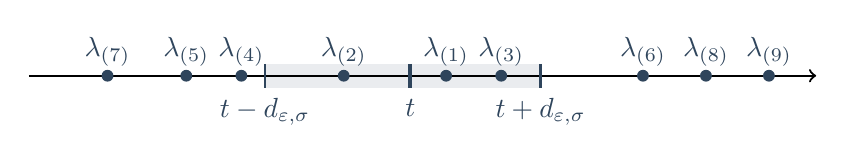
\begin{tikzpicture}
    \fill[lightblue] (-2, -0.15) rectangle (1.5, 0.15);
    \draw[thick, ->] (-5, 0) to (5, 0);
    \fill[darkblue] (-4, 0) circle (0.075) node[above] {$\lambda_{(7)}$};
    \fill[darkblue] (-3, 0) circle (0.075) node[above] {$\lambda_{(5)}$};
    \fill[darkblue] (-2.3, 0) circle (0.075) node[above] {$\lambda_{(4)}$};
    \fill[darkblue] (-1, 0) circle (0.075) node[above] {$\lambda_{(2)}$};
    \fill[darkblue] (0.3, 0) circle (0.075) node[above] {$\lambda_{(1)}$};
    \fill[darkblue] (1, 0) circle (0.075) node[above] {$\lambda_{(3)}$};
    \fill[darkblue] (2.8, 0) circle (0.075) node[above] {$\lambda_{(6)}$};
    \fill[darkblue] (3.6, 0) circle (0.075) node[above] {$\lambda_{(8)}$};
    \fill[darkblue] (4.4, 0) circle (0.075) node[above] {$\lambda_{(9)}$};
    \draw[darkblue, ultra thick] (-0.155, 0.15) to (-0.155, -0.15) node[below] {$t$};
    \draw[darkblue, thick] (-2, 0.15) to (-2, -0.15) node[below] {$t - d_{\varepsilon, \sigma}$};
    \draw[darkblue, thick] (1.5, 0.15) to (1.5, -0.15) node[below] {$t + d_{\varepsilon, \sigma}$};
\end{tikzpicture}
    \caption{The numerical rank of $g_{\sigma}(t\mtx{I}_n - \mtx{A}) / n$ can be approximately computed by counting the number of eigenvalues $\lambda_{(1)}, \dots, \lambda_{(n)}$ of the matrix $\mtx{A}$ which lie less than a constant $d_{\varepsilon, \sigma}$ away from $t$.}
    \label{fig:numerical-rank}
\end{figure}

If we additionally assume the eigenvalues of the matrix $\mtx{A}$ to be evenly distributed within $[-1, 1]$, that is, in any subinterval of fixed length in $[a, b]$, $-1 \leq a < b \leq 1$, we can expect to find roughly the same number of eigenvalues, then we can estimate the numerical rank of $g_{\sigma}(t\mtx{I}_n - \mtx{A}) / n$ to be
\begin{equation}
    r_{\varepsilon}(g_{\sigma}(t\mtx{I}_n - \mtx{A}) / n) \lessapprox n d_{\varepsilon, \sigma} \approx 6 n \sigma,
    \label{equ:gaussian-kernel-numerical-rank-uniform}
\end{equation}
provided we set $\varepsilon = 10^{-16}$ and choose $\sigma$ roughly between $10^{-8}$ and $1$. Hence, choosing $n_{\mtx{\Omega}} = \mathcal{O}(n \sigma)$ will yield approximations which can be significantly better than \refthm{thm:chebyshev-nystrom}.


\section{Numerical experiments}
\label{sec:results}

\subsection{Spectral density for Hamiltonian of electronic structure}
\label{subsec:hamiltonian}

Our first numerical example comes from electronic structure interaction \cite{lin-2017-randomized-estimation}, more precisely from the second order finite difference discretization of the Hamiltonian
\begin{equation}
    \mathcal{H} = - \Delta + V
    \label{equ:5-experiments-electronic-hamiltonian}
\end{equation}
in three dimensions. The potential $V$ interacting with the electrons is generated by Gaussian wells
\begin{equation}
    v(r) = v_0 e^{-\lambda r^2}
    \label{equ:5-experiments-gaussian-cell}
\end{equation}
with $v_0 = -4$ and $\lambda = 8$, centered in cells of side length $L=6$ which are stacked $n_c \in \mathbb{N}$ times in each spatial dimension (cf. \reffig{fig:gaussian-well}). The discretization step is fixed to be $h=0.6$, such that the size of the matrix grows cubically with $n_c$. This is an idealized model for the interaction of nuclei on a regular grid with electrons for a $k$-vector in the center of the first Brillouin zone. The distribution of the eigenvalues of the Hamiltonian -- its spectral density -- allows us to interpret the system's energy levels.

\begin{figure}[ht]
    \begin{subfigure}[b]{0.32\columnwidth}
        %% Creator: Matplotlib, PGF backend
%%
%% To include the figure in your LaTeX document, write
%%   \input{<filename>.pgf}
%%
%% Make sure the required packages are loaded in your preamble
%%   \usepackage{pgf}
%%
%% Also ensure that all the required font packages are loaded; for instance,
%% the lmodern package is sometimes necessary when using math font.
%%   \usepackage{lmodern}
%%
%% Figures using additional raster images can only be included by \input if
%% they are in the same directory as the main LaTeX file. For loading figures
%% from other directories you can use the `import` package
%%   \usepackage{import}
%%
%% and then include the figures with
%%   \import{<path to file>}{<filename>.pgf}
%%
%% Matplotlib used the following preamble
%%   \def\mathdefault#1{#1}
%%   \everymath=\expandafter{\the\everymath\displaystyle}
%%   
%%   \makeatletter\@ifpackageloaded{underscore}{}{\usepackage[strings]{underscore}}\makeatother
%%
\begingroup%
\makeatletter%
\begin{pgfpicture}%
\pgfpathrectangle{\pgfpointorigin}{\pgfqpoint{1.969617in}{1.850740in}}%
\pgfusepath{use as bounding box, clip}%
\begin{pgfscope}%
\pgfsetbuttcap%
\pgfsetmiterjoin%
\definecolor{currentfill}{rgb}{1.000000,1.000000,1.000000}%
\pgfsetfillcolor{currentfill}%
\pgfsetlinewidth{0.000000pt}%
\definecolor{currentstroke}{rgb}{1.000000,1.000000,1.000000}%
\pgfsetstrokecolor{currentstroke}%
\pgfsetdash{}{0pt}%
\pgfpathmoveto{\pgfqpoint{0.000000in}{0.000000in}}%
\pgfpathlineto{\pgfqpoint{1.969617in}{0.000000in}}%
\pgfpathlineto{\pgfqpoint{1.969617in}{1.850740in}}%
\pgfpathlineto{\pgfqpoint{0.000000in}{1.850740in}}%
\pgfpathlineto{\pgfqpoint{0.000000in}{0.000000in}}%
\pgfpathclose%
\pgfusepath{fill}%
\end{pgfscope}%
\begin{pgfscope}%
\pgfsetbuttcap%
\pgfsetmiterjoin%
\definecolor{currentfill}{rgb}{1.000000,1.000000,1.000000}%
\pgfsetfillcolor{currentfill}%
\pgfsetlinewidth{0.000000pt}%
\definecolor{currentstroke}{rgb}{0.000000,0.000000,0.000000}%
\pgfsetstrokecolor{currentstroke}%
\pgfsetstrokeopacity{0.000000}%
\pgfsetdash{}{0pt}%
\pgfpathmoveto{\pgfqpoint{0.278819in}{0.345370in}}%
\pgfpathlineto{\pgfqpoint{1.828819in}{0.345370in}}%
\pgfpathlineto{\pgfqpoint{1.828819in}{1.692870in}}%
\pgfpathlineto{\pgfqpoint{0.278819in}{1.692870in}}%
\pgfpathlineto{\pgfqpoint{0.278819in}{0.345370in}}%
\pgfpathclose%
\pgfusepath{fill}%
\end{pgfscope}%
\begin{pgfscope}%
\pgfpathrectangle{\pgfqpoint{0.278819in}{0.345370in}}{\pgfqpoint{1.550000in}{1.347500in}}%
\pgfusepath{clip}%
\pgfsetbuttcap%
\pgfsetroundjoin%
\definecolor{currentfill}{rgb}{0.993545,0.862859,0.619299}%
\pgfsetfillcolor{currentfill}%
\pgfsetlinewidth{0.000000pt}%
\definecolor{currentstroke}{rgb}{0.000000,0.000000,0.000000}%
\pgfsetstrokecolor{currentstroke}%
\pgfsetdash{}{0pt}%
\pgfpathmoveto{\pgfqpoint{1.014677in}{0.873327in}}%
\pgfpathlineto{\pgfqpoint{1.030334in}{0.870750in}}%
\pgfpathlineto{\pgfqpoint{1.045990in}{0.869462in}}%
\pgfpathlineto{\pgfqpoint{1.061647in}{0.869462in}}%
\pgfpathlineto{\pgfqpoint{1.077303in}{0.870750in}}%
\pgfpathlineto{\pgfqpoint{1.092960in}{0.873327in}}%
\pgfpathlineto{\pgfqpoint{1.104615in}{0.876203in}}%
\pgfpathlineto{\pgfqpoint{1.108617in}{0.877276in}}%
\pgfpathlineto{\pgfqpoint{1.124273in}{0.882865in}}%
\pgfpathlineto{\pgfqpoint{1.139841in}{0.889814in}}%
\pgfpathlineto{\pgfqpoint{1.139930in}{0.889858in}}%
\pgfpathlineto{\pgfqpoint{1.155586in}{0.899059in}}%
\pgfpathlineto{\pgfqpoint{1.161972in}{0.903425in}}%
\pgfpathlineto{\pgfqpoint{1.171243in}{0.910510in}}%
\pgfpathlineto{\pgfqpoint{1.178750in}{0.917036in}}%
\pgfpathlineto{\pgfqpoint{1.186899in}{0.925096in}}%
\pgfpathlineto{\pgfqpoint{1.191922in}{0.930648in}}%
\pgfpathlineto{\pgfqpoint{1.202506in}{0.944259in}}%
\pgfpathlineto{\pgfqpoint{1.202556in}{0.944336in}}%
\pgfpathlineto{\pgfqpoint{1.210550in}{0.957870in}}%
\pgfpathlineto{\pgfqpoint{1.216979in}{0.971481in}}%
\pgfpathlineto{\pgfqpoint{1.218213in}{0.974959in}}%
\pgfpathlineto{\pgfqpoint{1.221521in}{0.985092in}}%
\pgfpathlineto{\pgfqpoint{1.224485in}{0.998703in}}%
\pgfpathlineto{\pgfqpoint{1.225967in}{1.012314in}}%
\pgfpathlineto{\pgfqpoint{1.225967in}{1.025925in}}%
\pgfpathlineto{\pgfqpoint{1.224485in}{1.039536in}}%
\pgfpathlineto{\pgfqpoint{1.221521in}{1.053148in}}%
\pgfpathlineto{\pgfqpoint{1.218213in}{1.063280in}}%
\pgfpathlineto{\pgfqpoint{1.216979in}{1.066759in}}%
\pgfpathlineto{\pgfqpoint{1.210550in}{1.080370in}}%
\pgfpathlineto{\pgfqpoint{1.202556in}{1.093903in}}%
\pgfpathlineto{\pgfqpoint{1.202506in}{1.093981in}}%
\pgfpathlineto{\pgfqpoint{1.191922in}{1.107592in}}%
\pgfpathlineto{\pgfqpoint{1.186899in}{1.113143in}}%
\pgfpathlineto{\pgfqpoint{1.178750in}{1.121203in}}%
\pgfpathlineto{\pgfqpoint{1.171243in}{1.127729in}}%
\pgfpathlineto{\pgfqpoint{1.161972in}{1.134814in}}%
\pgfpathlineto{\pgfqpoint{1.155586in}{1.139181in}}%
\pgfpathlineto{\pgfqpoint{1.139930in}{1.148381in}}%
\pgfpathlineto{\pgfqpoint{1.139841in}{1.148425in}}%
\pgfpathlineto{\pgfqpoint{1.124273in}{1.155375in}}%
\pgfpathlineto{\pgfqpoint{1.108617in}{1.160964in}}%
\pgfpathlineto{\pgfqpoint{1.104615in}{1.162036in}}%
\pgfpathlineto{\pgfqpoint{1.092960in}{1.164913in}}%
\pgfpathlineto{\pgfqpoint{1.077303in}{1.167489in}}%
\pgfpathlineto{\pgfqpoint{1.061647in}{1.168777in}}%
\pgfpathlineto{\pgfqpoint{1.045990in}{1.168777in}}%
\pgfpathlineto{\pgfqpoint{1.030334in}{1.167489in}}%
\pgfpathlineto{\pgfqpoint{1.014677in}{1.164913in}}%
\pgfpathlineto{\pgfqpoint{1.003022in}{1.162036in}}%
\pgfpathlineto{\pgfqpoint{0.999021in}{1.160964in}}%
\pgfpathlineto{\pgfqpoint{0.983364in}{1.155375in}}%
\pgfpathlineto{\pgfqpoint{0.967797in}{1.148425in}}%
\pgfpathlineto{\pgfqpoint{0.967708in}{1.148381in}}%
\pgfpathlineto{\pgfqpoint{0.952051in}{1.139181in}}%
\pgfpathlineto{\pgfqpoint{0.945666in}{1.134814in}}%
\pgfpathlineto{\pgfqpoint{0.936394in}{1.127729in}}%
\pgfpathlineto{\pgfqpoint{0.928888in}{1.121203in}}%
\pgfpathlineto{\pgfqpoint{0.920738in}{1.113143in}}%
\pgfpathlineto{\pgfqpoint{0.915715in}{1.107592in}}%
\pgfpathlineto{\pgfqpoint{0.905132in}{1.093981in}}%
\pgfpathlineto{\pgfqpoint{0.905081in}{1.093903in}}%
\pgfpathlineto{\pgfqpoint{0.897088in}{1.080370in}}%
\pgfpathlineto{\pgfqpoint{0.890659in}{1.066759in}}%
\pgfpathlineto{\pgfqpoint{0.889425in}{1.063280in}}%
\pgfpathlineto{\pgfqpoint{0.886116in}{1.053148in}}%
\pgfpathlineto{\pgfqpoint{0.883152in}{1.039536in}}%
\pgfpathlineto{\pgfqpoint{0.881671in}{1.025925in}}%
\pgfpathlineto{\pgfqpoint{0.881671in}{1.012314in}}%
\pgfpathlineto{\pgfqpoint{0.883152in}{0.998703in}}%
\pgfpathlineto{\pgfqpoint{0.886116in}{0.985092in}}%
\pgfpathlineto{\pgfqpoint{0.889425in}{0.974959in}}%
\pgfpathlineto{\pgfqpoint{0.890659in}{0.971481in}}%
\pgfpathlineto{\pgfqpoint{0.897088in}{0.957870in}}%
\pgfpathlineto{\pgfqpoint{0.905081in}{0.944336in}}%
\pgfpathlineto{\pgfqpoint{0.905132in}{0.944259in}}%
\pgfpathlineto{\pgfqpoint{0.915715in}{0.930648in}}%
\pgfpathlineto{\pgfqpoint{0.920738in}{0.925096in}}%
\pgfpathlineto{\pgfqpoint{0.928888in}{0.917036in}}%
\pgfpathlineto{\pgfqpoint{0.936394in}{0.910510in}}%
\pgfpathlineto{\pgfqpoint{0.945666in}{0.903425in}}%
\pgfpathlineto{\pgfqpoint{0.952051in}{0.899059in}}%
\pgfpathlineto{\pgfqpoint{0.967708in}{0.889858in}}%
\pgfpathlineto{\pgfqpoint{0.967797in}{0.889814in}}%
\pgfpathlineto{\pgfqpoint{0.983364in}{0.882865in}}%
\pgfpathlineto{\pgfqpoint{0.999021in}{0.877276in}}%
\pgfpathlineto{\pgfqpoint{1.003022in}{0.876203in}}%
\pgfpathlineto{\pgfqpoint{1.014677in}{0.873327in}}%
\pgfpathclose%
\pgfusepath{fill}%
\end{pgfscope}%
\begin{pgfscope}%
\pgfpathrectangle{\pgfqpoint{0.278819in}{0.345370in}}{\pgfqpoint{1.550000in}{1.347500in}}%
\pgfusepath{clip}%
\pgfsetbuttcap%
\pgfsetroundjoin%
\definecolor{currentfill}{rgb}{0.993326,0.602275,0.414390}%
\pgfsetfillcolor{currentfill}%
\pgfsetlinewidth{0.000000pt}%
\definecolor{currentstroke}{rgb}{0.000000,0.000000,0.000000}%
\pgfsetstrokecolor{currentstroke}%
\pgfsetdash{}{0pt}%
\pgfpathmoveto{\pgfqpoint{0.999021in}{0.739415in}}%
\pgfpathlineto{\pgfqpoint{1.014677in}{0.737106in}}%
\pgfpathlineto{\pgfqpoint{1.030334in}{0.735568in}}%
\pgfpathlineto{\pgfqpoint{1.045990in}{0.734799in}}%
\pgfpathlineto{\pgfqpoint{1.061647in}{0.734799in}}%
\pgfpathlineto{\pgfqpoint{1.077303in}{0.735568in}}%
\pgfpathlineto{\pgfqpoint{1.092960in}{0.737106in}}%
\pgfpathlineto{\pgfqpoint{1.108617in}{0.739415in}}%
\pgfpathlineto{\pgfqpoint{1.112069in}{0.740092in}}%
\pgfpathlineto{\pgfqpoint{1.124273in}{0.742535in}}%
\pgfpathlineto{\pgfqpoint{1.139930in}{0.746452in}}%
\pgfpathlineto{\pgfqpoint{1.155586in}{0.751154in}}%
\pgfpathlineto{\pgfqpoint{1.162877in}{0.753703in}}%
\pgfpathlineto{\pgfqpoint{1.171243in}{0.756707in}}%
\pgfpathlineto{\pgfqpoint{1.186899in}{0.763121in}}%
\pgfpathlineto{\pgfqpoint{1.196020in}{0.767314in}}%
\pgfpathlineto{\pgfqpoint{1.202556in}{0.770419in}}%
\pgfpathlineto{\pgfqpoint{1.218213in}{0.778656in}}%
\pgfpathlineto{\pgfqpoint{1.222157in}{0.780925in}}%
\pgfpathlineto{\pgfqpoint{1.233869in}{0.787933in}}%
\pgfpathlineto{\pgfqpoint{1.244037in}{0.794536in}}%
\pgfpathlineto{\pgfqpoint{1.249526in}{0.798265in}}%
\pgfpathlineto{\pgfqpoint{1.263051in}{0.808148in}}%
\pgfpathlineto{\pgfqpoint{1.265182in}{0.809786in}}%
\pgfpathlineto{\pgfqpoint{1.279772in}{0.821759in}}%
\pgfpathlineto{\pgfqpoint{1.280839in}{0.822686in}}%
\pgfpathlineto{\pgfqpoint{1.294610in}{0.835370in}}%
\pgfpathlineto{\pgfqpoint{1.296495in}{0.837223in}}%
\pgfpathlineto{\pgfqpoint{1.307864in}{0.848981in}}%
\pgfpathlineto{\pgfqpoint{1.312152in}{0.853753in}}%
\pgfpathlineto{\pgfqpoint{1.319748in}{0.862592in}}%
\pgfpathlineto{\pgfqpoint{1.327809in}{0.872774in}}%
\pgfpathlineto{\pgfqpoint{1.330419in}{0.876203in}}%
\pgfpathlineto{\pgfqpoint{1.339893in}{0.889814in}}%
\pgfpathlineto{\pgfqpoint{1.343465in}{0.895496in}}%
\pgfpathlineto{\pgfqpoint{1.348289in}{0.903425in}}%
\pgfpathlineto{\pgfqpoint{1.355666in}{0.917036in}}%
\pgfpathlineto{\pgfqpoint{1.359122in}{0.924309in}}%
\pgfpathlineto{\pgfqpoint{1.362054in}{0.930648in}}%
\pgfpathlineto{\pgfqpoint{1.367463in}{0.944259in}}%
\pgfpathlineto{\pgfqpoint{1.371968in}{0.957870in}}%
\pgfpathlineto{\pgfqpoint{1.374778in}{0.968479in}}%
\pgfpathlineto{\pgfqpoint{1.375557in}{0.971481in}}%
\pgfpathlineto{\pgfqpoint{1.378212in}{0.985092in}}%
\pgfpathlineto{\pgfqpoint{1.379982in}{0.998703in}}%
\pgfpathlineto{\pgfqpoint{1.380866in}{1.012314in}}%
\pgfpathlineto{\pgfqpoint{1.380866in}{1.025925in}}%
\pgfpathlineto{\pgfqpoint{1.379982in}{1.039536in}}%
\pgfpathlineto{\pgfqpoint{1.378212in}{1.053148in}}%
\pgfpathlineto{\pgfqpoint{1.375557in}{1.066759in}}%
\pgfpathlineto{\pgfqpoint{1.374778in}{1.069760in}}%
\pgfpathlineto{\pgfqpoint{1.371968in}{1.080370in}}%
\pgfpathlineto{\pgfqpoint{1.367463in}{1.093981in}}%
\pgfpathlineto{\pgfqpoint{1.362054in}{1.107592in}}%
\pgfpathlineto{\pgfqpoint{1.359122in}{1.113930in}}%
\pgfpathlineto{\pgfqpoint{1.355666in}{1.121203in}}%
\pgfpathlineto{\pgfqpoint{1.348289in}{1.134814in}}%
\pgfpathlineto{\pgfqpoint{1.343465in}{1.142743in}}%
\pgfpathlineto{\pgfqpoint{1.339893in}{1.148425in}}%
\pgfpathlineto{\pgfqpoint{1.330419in}{1.162036in}}%
\pgfpathlineto{\pgfqpoint{1.327809in}{1.165465in}}%
\pgfpathlineto{\pgfqpoint{1.319748in}{1.175647in}}%
\pgfpathlineto{\pgfqpoint{1.312152in}{1.184487in}}%
\pgfpathlineto{\pgfqpoint{1.307864in}{1.189259in}}%
\pgfpathlineto{\pgfqpoint{1.296495in}{1.201017in}}%
\pgfpathlineto{\pgfqpoint{1.294610in}{1.202870in}}%
\pgfpathlineto{\pgfqpoint{1.280839in}{1.215553in}}%
\pgfpathlineto{\pgfqpoint{1.279772in}{1.216481in}}%
\pgfpathlineto{\pgfqpoint{1.265182in}{1.228453in}}%
\pgfpathlineto{\pgfqpoint{1.263051in}{1.230092in}}%
\pgfpathlineto{\pgfqpoint{1.249526in}{1.239975in}}%
\pgfpathlineto{\pgfqpoint{1.244037in}{1.243703in}}%
\pgfpathlineto{\pgfqpoint{1.233869in}{1.250307in}}%
\pgfpathlineto{\pgfqpoint{1.222157in}{1.257314in}}%
\pgfpathlineto{\pgfqpoint{1.218213in}{1.259584in}}%
\pgfpathlineto{\pgfqpoint{1.202556in}{1.267820in}}%
\pgfpathlineto{\pgfqpoint{1.196020in}{1.270925in}}%
\pgfpathlineto{\pgfqpoint{1.186899in}{1.275119in}}%
\pgfpathlineto{\pgfqpoint{1.171243in}{1.281532in}}%
\pgfpathlineto{\pgfqpoint{1.162877in}{1.284536in}}%
\pgfpathlineto{\pgfqpoint{1.155586in}{1.287085in}}%
\pgfpathlineto{\pgfqpoint{1.139930in}{1.291788in}}%
\pgfpathlineto{\pgfqpoint{1.124273in}{1.295705in}}%
\pgfpathlineto{\pgfqpoint{1.112069in}{1.298148in}}%
\pgfpathlineto{\pgfqpoint{1.108617in}{1.298825in}}%
\pgfpathlineto{\pgfqpoint{1.092960in}{1.301133in}}%
\pgfpathlineto{\pgfqpoint{1.077303in}{1.302671in}}%
\pgfpathlineto{\pgfqpoint{1.061647in}{1.303440in}}%
\pgfpathlineto{\pgfqpoint{1.045990in}{1.303440in}}%
\pgfpathlineto{\pgfqpoint{1.030334in}{1.302671in}}%
\pgfpathlineto{\pgfqpoint{1.014677in}{1.301133in}}%
\pgfpathlineto{\pgfqpoint{0.999021in}{1.298825in}}%
\pgfpathlineto{\pgfqpoint{0.995568in}{1.298148in}}%
\pgfpathlineto{\pgfqpoint{0.983364in}{1.295705in}}%
\pgfpathlineto{\pgfqpoint{0.967708in}{1.291788in}}%
\pgfpathlineto{\pgfqpoint{0.952051in}{1.287085in}}%
\pgfpathlineto{\pgfqpoint{0.944760in}{1.284536in}}%
\pgfpathlineto{\pgfqpoint{0.936394in}{1.281532in}}%
\pgfpathlineto{\pgfqpoint{0.920738in}{1.275119in}}%
\pgfpathlineto{\pgfqpoint{0.911617in}{1.270925in}}%
\pgfpathlineto{\pgfqpoint{0.905081in}{1.267820in}}%
\pgfpathlineto{\pgfqpoint{0.889425in}{1.259584in}}%
\pgfpathlineto{\pgfqpoint{0.885481in}{1.257314in}}%
\pgfpathlineto{\pgfqpoint{0.873768in}{1.250307in}}%
\pgfpathlineto{\pgfqpoint{0.863600in}{1.243703in}}%
\pgfpathlineto{\pgfqpoint{0.858112in}{1.239975in}}%
\pgfpathlineto{\pgfqpoint{0.844586in}{1.230092in}}%
\pgfpathlineto{\pgfqpoint{0.842455in}{1.228453in}}%
\pgfpathlineto{\pgfqpoint{0.827865in}{1.216481in}}%
\pgfpathlineto{\pgfqpoint{0.826798in}{1.215553in}}%
\pgfpathlineto{\pgfqpoint{0.813027in}{1.202870in}}%
\pgfpathlineto{\pgfqpoint{0.811142in}{1.201017in}}%
\pgfpathlineto{\pgfqpoint{0.799774in}{1.189259in}}%
\pgfpathlineto{\pgfqpoint{0.795485in}{1.184487in}}%
\pgfpathlineto{\pgfqpoint{0.787889in}{1.175647in}}%
\pgfpathlineto{\pgfqpoint{0.779829in}{1.165465in}}%
\pgfpathlineto{\pgfqpoint{0.777218in}{1.162036in}}%
\pgfpathlineto{\pgfqpoint{0.767744in}{1.148425in}}%
\pgfpathlineto{\pgfqpoint{0.764172in}{1.142743in}}%
\pgfpathlineto{\pgfqpoint{0.759348in}{1.134814in}}%
\pgfpathlineto{\pgfqpoint{0.751971in}{1.121203in}}%
\pgfpathlineto{\pgfqpoint{0.748516in}{1.113930in}}%
\pgfpathlineto{\pgfqpoint{0.745583in}{1.107592in}}%
\pgfpathlineto{\pgfqpoint{0.740174in}{1.093981in}}%
\pgfpathlineto{\pgfqpoint{0.735669in}{1.080370in}}%
\pgfpathlineto{\pgfqpoint{0.732859in}{1.069760in}}%
\pgfpathlineto{\pgfqpoint{0.732080in}{1.066759in}}%
\pgfpathlineto{\pgfqpoint{0.729425in}{1.053148in}}%
\pgfpathlineto{\pgfqpoint{0.727655in}{1.039536in}}%
\pgfpathlineto{\pgfqpoint{0.726771in}{1.025925in}}%
\pgfpathlineto{\pgfqpoint{0.726771in}{1.012314in}}%
\pgfpathlineto{\pgfqpoint{0.727655in}{0.998703in}}%
\pgfpathlineto{\pgfqpoint{0.729425in}{0.985092in}}%
\pgfpathlineto{\pgfqpoint{0.732080in}{0.971481in}}%
\pgfpathlineto{\pgfqpoint{0.732859in}{0.968479in}}%
\pgfpathlineto{\pgfqpoint{0.735669in}{0.957870in}}%
\pgfpathlineto{\pgfqpoint{0.740174in}{0.944259in}}%
\pgfpathlineto{\pgfqpoint{0.745583in}{0.930647in}}%
\pgfpathlineto{\pgfqpoint{0.748516in}{0.924309in}}%
\pgfpathlineto{\pgfqpoint{0.751971in}{0.917036in}}%
\pgfpathlineto{\pgfqpoint{0.759348in}{0.903425in}}%
\pgfpathlineto{\pgfqpoint{0.764172in}{0.895496in}}%
\pgfpathlineto{\pgfqpoint{0.767744in}{0.889814in}}%
\pgfpathlineto{\pgfqpoint{0.777218in}{0.876203in}}%
\pgfpathlineto{\pgfqpoint{0.779829in}{0.872774in}}%
\pgfpathlineto{\pgfqpoint{0.787889in}{0.862592in}}%
\pgfpathlineto{\pgfqpoint{0.795485in}{0.853753in}}%
\pgfpathlineto{\pgfqpoint{0.799774in}{0.848981in}}%
\pgfpathlineto{\pgfqpoint{0.811142in}{0.837223in}}%
\pgfpathlineto{\pgfqpoint{0.813027in}{0.835370in}}%
\pgfpathlineto{\pgfqpoint{0.826798in}{0.822686in}}%
\pgfpathlineto{\pgfqpoint{0.827865in}{0.821759in}}%
\pgfpathlineto{\pgfqpoint{0.842455in}{0.809786in}}%
\pgfpathlineto{\pgfqpoint{0.844586in}{0.808148in}}%
\pgfpathlineto{\pgfqpoint{0.858112in}{0.798265in}}%
\pgfpathlineto{\pgfqpoint{0.863600in}{0.794536in}}%
\pgfpathlineto{\pgfqpoint{0.873768in}{0.787933in}}%
\pgfpathlineto{\pgfqpoint{0.885481in}{0.780925in}}%
\pgfpathlineto{\pgfqpoint{0.889425in}{0.778656in}}%
\pgfpathlineto{\pgfqpoint{0.905081in}{0.770419in}}%
\pgfpathlineto{\pgfqpoint{0.911617in}{0.767314in}}%
\pgfpathlineto{\pgfqpoint{0.920738in}{0.763121in}}%
\pgfpathlineto{\pgfqpoint{0.936394in}{0.756707in}}%
\pgfpathlineto{\pgfqpoint{0.944760in}{0.753703in}}%
\pgfpathlineto{\pgfqpoint{0.952051in}{0.751154in}}%
\pgfpathlineto{\pgfqpoint{0.967708in}{0.746452in}}%
\pgfpathlineto{\pgfqpoint{0.983364in}{0.742535in}}%
\pgfpathlineto{\pgfqpoint{0.995568in}{0.740092in}}%
\pgfpathlineto{\pgfqpoint{0.999021in}{0.739415in}}%
\pgfpathclose%
\pgfpathmoveto{\pgfqpoint{1.003022in}{0.876203in}}%
\pgfpathlineto{\pgfqpoint{0.999021in}{0.877276in}}%
\pgfpathlineto{\pgfqpoint{0.983364in}{0.882865in}}%
\pgfpathlineto{\pgfqpoint{0.967797in}{0.889814in}}%
\pgfpathlineto{\pgfqpoint{0.967708in}{0.889858in}}%
\pgfpathlineto{\pgfqpoint{0.952051in}{0.899059in}}%
\pgfpathlineto{\pgfqpoint{0.945666in}{0.903425in}}%
\pgfpathlineto{\pgfqpoint{0.936394in}{0.910510in}}%
\pgfpathlineto{\pgfqpoint{0.928888in}{0.917036in}}%
\pgfpathlineto{\pgfqpoint{0.920738in}{0.925096in}}%
\pgfpathlineto{\pgfqpoint{0.915715in}{0.930648in}}%
\pgfpathlineto{\pgfqpoint{0.905132in}{0.944259in}}%
\pgfpathlineto{\pgfqpoint{0.905081in}{0.944336in}}%
\pgfpathlineto{\pgfqpoint{0.897088in}{0.957870in}}%
\pgfpathlineto{\pgfqpoint{0.890659in}{0.971481in}}%
\pgfpathlineto{\pgfqpoint{0.889425in}{0.974959in}}%
\pgfpathlineto{\pgfqpoint{0.886116in}{0.985092in}}%
\pgfpathlineto{\pgfqpoint{0.883152in}{0.998703in}}%
\pgfpathlineto{\pgfqpoint{0.881671in}{1.012314in}}%
\pgfpathlineto{\pgfqpoint{0.881671in}{1.025925in}}%
\pgfpathlineto{\pgfqpoint{0.883152in}{1.039536in}}%
\pgfpathlineto{\pgfqpoint{0.886116in}{1.053148in}}%
\pgfpathlineto{\pgfqpoint{0.889425in}{1.063280in}}%
\pgfpathlineto{\pgfqpoint{0.890659in}{1.066759in}}%
\pgfpathlineto{\pgfqpoint{0.897088in}{1.080370in}}%
\pgfpathlineto{\pgfqpoint{0.905081in}{1.093903in}}%
\pgfpathlineto{\pgfqpoint{0.905132in}{1.093981in}}%
\pgfpathlineto{\pgfqpoint{0.915715in}{1.107592in}}%
\pgfpathlineto{\pgfqpoint{0.920738in}{1.113143in}}%
\pgfpathlineto{\pgfqpoint{0.928888in}{1.121203in}}%
\pgfpathlineto{\pgfqpoint{0.936394in}{1.127729in}}%
\pgfpathlineto{\pgfqpoint{0.945666in}{1.134814in}}%
\pgfpathlineto{\pgfqpoint{0.952051in}{1.139181in}}%
\pgfpathlineto{\pgfqpoint{0.967708in}{1.148381in}}%
\pgfpathlineto{\pgfqpoint{0.967797in}{1.148425in}}%
\pgfpathlineto{\pgfqpoint{0.983364in}{1.155375in}}%
\pgfpathlineto{\pgfqpoint{0.999021in}{1.160964in}}%
\pgfpathlineto{\pgfqpoint{1.003022in}{1.162036in}}%
\pgfpathlineto{\pgfqpoint{1.014677in}{1.164913in}}%
\pgfpathlineto{\pgfqpoint{1.030334in}{1.167489in}}%
\pgfpathlineto{\pgfqpoint{1.045990in}{1.168777in}}%
\pgfpathlineto{\pgfqpoint{1.061647in}{1.168777in}}%
\pgfpathlineto{\pgfqpoint{1.077303in}{1.167489in}}%
\pgfpathlineto{\pgfqpoint{1.092960in}{1.164913in}}%
\pgfpathlineto{\pgfqpoint{1.104615in}{1.162036in}}%
\pgfpathlineto{\pgfqpoint{1.108617in}{1.160964in}}%
\pgfpathlineto{\pgfqpoint{1.124273in}{1.155375in}}%
\pgfpathlineto{\pgfqpoint{1.139841in}{1.148425in}}%
\pgfpathlineto{\pgfqpoint{1.139930in}{1.148381in}}%
\pgfpathlineto{\pgfqpoint{1.155586in}{1.139181in}}%
\pgfpathlineto{\pgfqpoint{1.161972in}{1.134814in}}%
\pgfpathlineto{\pgfqpoint{1.171243in}{1.127729in}}%
\pgfpathlineto{\pgfqpoint{1.178750in}{1.121203in}}%
\pgfpathlineto{\pgfqpoint{1.186899in}{1.113143in}}%
\pgfpathlineto{\pgfqpoint{1.191922in}{1.107592in}}%
\pgfpathlineto{\pgfqpoint{1.202506in}{1.093981in}}%
\pgfpathlineto{\pgfqpoint{1.202556in}{1.093903in}}%
\pgfpathlineto{\pgfqpoint{1.210550in}{1.080370in}}%
\pgfpathlineto{\pgfqpoint{1.216979in}{1.066759in}}%
\pgfpathlineto{\pgfqpoint{1.218213in}{1.063280in}}%
\pgfpathlineto{\pgfqpoint{1.221521in}{1.053148in}}%
\pgfpathlineto{\pgfqpoint{1.224485in}{1.039536in}}%
\pgfpathlineto{\pgfqpoint{1.225967in}{1.025925in}}%
\pgfpathlineto{\pgfqpoint{1.225967in}{1.012314in}}%
\pgfpathlineto{\pgfqpoint{1.224485in}{0.998703in}}%
\pgfpathlineto{\pgfqpoint{1.221521in}{0.985092in}}%
\pgfpathlineto{\pgfqpoint{1.218213in}{0.974959in}}%
\pgfpathlineto{\pgfqpoint{1.216979in}{0.971481in}}%
\pgfpathlineto{\pgfqpoint{1.210550in}{0.957870in}}%
\pgfpathlineto{\pgfqpoint{1.202556in}{0.944336in}}%
\pgfpathlineto{\pgfqpoint{1.202506in}{0.944259in}}%
\pgfpathlineto{\pgfqpoint{1.191922in}{0.930648in}}%
\pgfpathlineto{\pgfqpoint{1.186899in}{0.925096in}}%
\pgfpathlineto{\pgfqpoint{1.178750in}{0.917036in}}%
\pgfpathlineto{\pgfqpoint{1.171243in}{0.910510in}}%
\pgfpathlineto{\pgfqpoint{1.161972in}{0.903425in}}%
\pgfpathlineto{\pgfqpoint{1.155586in}{0.899059in}}%
\pgfpathlineto{\pgfqpoint{1.139930in}{0.889858in}}%
\pgfpathlineto{\pgfqpoint{1.139841in}{0.889814in}}%
\pgfpathlineto{\pgfqpoint{1.124273in}{0.882865in}}%
\pgfpathlineto{\pgfqpoint{1.108617in}{0.877276in}}%
\pgfpathlineto{\pgfqpoint{1.104615in}{0.876203in}}%
\pgfpathlineto{\pgfqpoint{1.092960in}{0.873327in}}%
\pgfpathlineto{\pgfqpoint{1.077303in}{0.870750in}}%
\pgfpathlineto{\pgfqpoint{1.061647in}{0.869462in}}%
\pgfpathlineto{\pgfqpoint{1.045990in}{0.869462in}}%
\pgfpathlineto{\pgfqpoint{1.030334in}{0.870750in}}%
\pgfpathlineto{\pgfqpoint{1.014677in}{0.873327in}}%
\pgfpathlineto{\pgfqpoint{1.003022in}{0.876203in}}%
\pgfpathclose%
\pgfusepath{fill}%
\end{pgfscope}%
\begin{pgfscope}%
\pgfpathrectangle{\pgfqpoint{0.278819in}{0.345370in}}{\pgfqpoint{1.550000in}{1.347500in}}%
\pgfusepath{clip}%
\pgfsetbuttcap%
\pgfsetroundjoin%
\definecolor{currentfill}{rgb}{0.921884,0.341098,0.377376}%
\pgfsetfillcolor{currentfill}%
\pgfsetlinewidth{0.000000pt}%
\definecolor{currentstroke}{rgb}{0.000000,0.000000,0.000000}%
\pgfsetstrokecolor{currentstroke}%
\pgfsetdash{}{0pt}%
\pgfpathmoveto{\pgfqpoint{0.967708in}{0.631202in}}%
\pgfpathlineto{\pgfqpoint{0.983364in}{0.627741in}}%
\pgfpathlineto{\pgfqpoint{0.999021in}{0.624975in}}%
\pgfpathlineto{\pgfqpoint{1.014677in}{0.622900in}}%
\pgfpathlineto{\pgfqpoint{1.030334in}{0.621518in}}%
\pgfpathlineto{\pgfqpoint{1.045990in}{0.620826in}}%
\pgfpathlineto{\pgfqpoint{1.061647in}{0.620826in}}%
\pgfpathlineto{\pgfqpoint{1.077303in}{0.621518in}}%
\pgfpathlineto{\pgfqpoint{1.092960in}{0.622900in}}%
\pgfpathlineto{\pgfqpoint{1.108617in}{0.624975in}}%
\pgfpathlineto{\pgfqpoint{1.124273in}{0.627741in}}%
\pgfpathlineto{\pgfqpoint{1.139930in}{0.631202in}}%
\pgfpathlineto{\pgfqpoint{1.139935in}{0.631203in}}%
\pgfpathlineto{\pgfqpoint{1.155586in}{0.635291in}}%
\pgfpathlineto{\pgfqpoint{1.171243in}{0.640064in}}%
\pgfpathlineto{\pgfqpoint{1.184880in}{0.644814in}}%
\pgfpathlineto{\pgfqpoint{1.186899in}{0.645513in}}%
\pgfpathlineto{\pgfqpoint{1.202556in}{0.651585in}}%
\pgfpathlineto{\pgfqpoint{1.218213in}{0.658335in}}%
\pgfpathlineto{\pgfqpoint{1.218405in}{0.658425in}}%
\pgfpathlineto{\pgfqpoint{1.233869in}{0.665706in}}%
\pgfpathlineto{\pgfqpoint{1.246218in}{0.672036in}}%
\pgfpathlineto{\pgfqpoint{1.249526in}{0.673741in}}%
\pgfpathlineto{\pgfqpoint{1.265182in}{0.682419in}}%
\pgfpathlineto{\pgfqpoint{1.270627in}{0.685648in}}%
\pgfpathlineto{\pgfqpoint{1.280839in}{0.691764in}}%
\pgfpathlineto{\pgfqpoint{1.292598in}{0.699259in}}%
\pgfpathlineto{\pgfqpoint{1.296495in}{0.701780in}}%
\pgfpathlineto{\pgfqpoint{1.312152in}{0.712485in}}%
\pgfpathlineto{\pgfqpoint{1.312688in}{0.712870in}}%
\pgfpathlineto{\pgfqpoint{1.327809in}{0.723931in}}%
\pgfpathlineto{\pgfqpoint{1.331141in}{0.726481in}}%
\pgfpathlineto{\pgfqpoint{1.343465in}{0.736144in}}%
\pgfpathlineto{\pgfqpoint{1.348306in}{0.740092in}}%
\pgfpathlineto{\pgfqpoint{1.359122in}{0.749177in}}%
\pgfpathlineto{\pgfqpoint{1.364327in}{0.753703in}}%
\pgfpathlineto{\pgfqpoint{1.374778in}{0.763106in}}%
\pgfpathlineto{\pgfqpoint{1.379320in}{0.767314in}}%
\pgfpathlineto{\pgfqpoint{1.390435in}{0.778028in}}%
\pgfpathlineto{\pgfqpoint{1.393367in}{0.780925in}}%
\pgfpathlineto{\pgfqpoint{1.406091in}{0.794070in}}%
\pgfpathlineto{\pgfqpoint{1.406534in}{0.794536in}}%
\pgfpathlineto{\pgfqpoint{1.418847in}{0.808148in}}%
\pgfpathlineto{\pgfqpoint{1.421748in}{0.811536in}}%
\pgfpathlineto{\pgfqpoint{1.430369in}{0.821759in}}%
\pgfpathlineto{\pgfqpoint{1.437404in}{0.830636in}}%
\pgfpathlineto{\pgfqpoint{1.441118in}{0.835370in}}%
\pgfpathlineto{\pgfqpoint{1.451101in}{0.848981in}}%
\pgfpathlineto{\pgfqpoint{1.453061in}{0.851856in}}%
\pgfpathlineto{\pgfqpoint{1.460343in}{0.862592in}}%
\pgfpathlineto{\pgfqpoint{1.468718in}{0.876036in}}%
\pgfpathlineto{\pgfqpoint{1.468822in}{0.876203in}}%
\pgfpathlineto{\pgfqpoint{1.476585in}{0.889814in}}%
\pgfpathlineto{\pgfqpoint{1.483570in}{0.903425in}}%
\pgfpathlineto{\pgfqpoint{1.484374in}{0.905180in}}%
\pgfpathlineto{\pgfqpoint{1.489838in}{0.917036in}}%
\pgfpathlineto{\pgfqpoint{1.495329in}{0.930648in}}%
\pgfpathlineto{\pgfqpoint{1.500031in}{0.944254in}}%
\pgfpathlineto{\pgfqpoint{1.500032in}{0.944259in}}%
\pgfpathlineto{\pgfqpoint{1.504013in}{0.957870in}}%
\pgfpathlineto{\pgfqpoint{1.507195in}{0.971481in}}%
\pgfpathlineto{\pgfqpoint{1.509581in}{0.985092in}}%
\pgfpathlineto{\pgfqpoint{1.511172in}{0.998703in}}%
\pgfpathlineto{\pgfqpoint{1.511967in}{1.012314in}}%
\pgfpathlineto{\pgfqpoint{1.511967in}{1.025925in}}%
\pgfpathlineto{\pgfqpoint{1.511172in}{1.039536in}}%
\pgfpathlineto{\pgfqpoint{1.509581in}{1.053148in}}%
\pgfpathlineto{\pgfqpoint{1.507195in}{1.066759in}}%
\pgfpathlineto{\pgfqpoint{1.504013in}{1.080370in}}%
\pgfpathlineto{\pgfqpoint{1.500032in}{1.093981in}}%
\pgfpathlineto{\pgfqpoint{1.500031in}{1.093986in}}%
\pgfpathlineto{\pgfqpoint{1.495329in}{1.107592in}}%
\pgfpathlineto{\pgfqpoint{1.489838in}{1.121203in}}%
\pgfpathlineto{\pgfqpoint{1.484374in}{1.133059in}}%
\pgfpathlineto{\pgfqpoint{1.483570in}{1.134814in}}%
\pgfpathlineto{\pgfqpoint{1.476585in}{1.148425in}}%
\pgfpathlineto{\pgfqpoint{1.468822in}{1.162036in}}%
\pgfpathlineto{\pgfqpoint{1.468718in}{1.162204in}}%
\pgfpathlineto{\pgfqpoint{1.460343in}{1.175647in}}%
\pgfpathlineto{\pgfqpoint{1.453061in}{1.186383in}}%
\pgfpathlineto{\pgfqpoint{1.451101in}{1.189259in}}%
\pgfpathlineto{\pgfqpoint{1.441118in}{1.202870in}}%
\pgfpathlineto{\pgfqpoint{1.437404in}{1.207603in}}%
\pgfpathlineto{\pgfqpoint{1.430369in}{1.216481in}}%
\pgfpathlineto{\pgfqpoint{1.421748in}{1.226703in}}%
\pgfpathlineto{\pgfqpoint{1.418847in}{1.230092in}}%
\pgfpathlineto{\pgfqpoint{1.406534in}{1.243703in}}%
\pgfpathlineto{\pgfqpoint{1.406091in}{1.244169in}}%
\pgfpathlineto{\pgfqpoint{1.393367in}{1.257314in}}%
\pgfpathlineto{\pgfqpoint{1.390435in}{1.260212in}}%
\pgfpathlineto{\pgfqpoint{1.379320in}{1.270925in}}%
\pgfpathlineto{\pgfqpoint{1.374778in}{1.275134in}}%
\pgfpathlineto{\pgfqpoint{1.364327in}{1.284536in}}%
\pgfpathlineto{\pgfqpoint{1.359122in}{1.289062in}}%
\pgfpathlineto{\pgfqpoint{1.348306in}{1.298148in}}%
\pgfpathlineto{\pgfqpoint{1.343465in}{1.302096in}}%
\pgfpathlineto{\pgfqpoint{1.331141in}{1.311759in}}%
\pgfpathlineto{\pgfqpoint{1.327809in}{1.314308in}}%
\pgfpathlineto{\pgfqpoint{1.312688in}{1.325370in}}%
\pgfpathlineto{\pgfqpoint{1.312152in}{1.325754in}}%
\pgfpathlineto{\pgfqpoint{1.296495in}{1.336459in}}%
\pgfpathlineto{\pgfqpoint{1.292598in}{1.338981in}}%
\pgfpathlineto{\pgfqpoint{1.280839in}{1.346475in}}%
\pgfpathlineto{\pgfqpoint{1.270627in}{1.352592in}}%
\pgfpathlineto{\pgfqpoint{1.265182in}{1.355820in}}%
\pgfpathlineto{\pgfqpoint{1.249526in}{1.364499in}}%
\pgfpathlineto{\pgfqpoint{1.246218in}{1.366203in}}%
\pgfpathlineto{\pgfqpoint{1.233869in}{1.372534in}}%
\pgfpathlineto{\pgfqpoint{1.218405in}{1.379814in}}%
\pgfpathlineto{\pgfqpoint{1.218213in}{1.379905in}}%
\pgfpathlineto{\pgfqpoint{1.202556in}{1.386654in}}%
\pgfpathlineto{\pgfqpoint{1.186899in}{1.392726in}}%
\pgfpathlineto{\pgfqpoint{1.184880in}{1.393425in}}%
\pgfpathlineto{\pgfqpoint{1.171243in}{1.398176in}}%
\pgfpathlineto{\pgfqpoint{1.155586in}{1.402949in}}%
\pgfpathlineto{\pgfqpoint{1.139935in}{1.407036in}}%
\pgfpathlineto{\pgfqpoint{1.139930in}{1.407038in}}%
\pgfpathlineto{\pgfqpoint{1.124273in}{1.410498in}}%
\pgfpathlineto{\pgfqpoint{1.108617in}{1.413265in}}%
\pgfpathlineto{\pgfqpoint{1.092960in}{1.415339in}}%
\pgfpathlineto{\pgfqpoint{1.077303in}{1.416722in}}%
\pgfpathlineto{\pgfqpoint{1.061647in}{1.417413in}}%
\pgfpathlineto{\pgfqpoint{1.045990in}{1.417413in}}%
\pgfpathlineto{\pgfqpoint{1.030334in}{1.416722in}}%
\pgfpathlineto{\pgfqpoint{1.014677in}{1.415339in}}%
\pgfpathlineto{\pgfqpoint{0.999021in}{1.413265in}}%
\pgfpathlineto{\pgfqpoint{0.983364in}{1.410498in}}%
\pgfpathlineto{\pgfqpoint{0.967707in}{1.407038in}}%
\pgfpathlineto{\pgfqpoint{0.967702in}{1.407036in}}%
\pgfpathlineto{\pgfqpoint{0.952051in}{1.402949in}}%
\pgfpathlineto{\pgfqpoint{0.936394in}{1.398176in}}%
\pgfpathlineto{\pgfqpoint{0.922757in}{1.393425in}}%
\pgfpathlineto{\pgfqpoint{0.920738in}{1.392726in}}%
\pgfpathlineto{\pgfqpoint{0.905081in}{1.386654in}}%
\pgfpathlineto{\pgfqpoint{0.889425in}{1.379905in}}%
\pgfpathlineto{\pgfqpoint{0.889232in}{1.379814in}}%
\pgfpathlineto{\pgfqpoint{0.873768in}{1.372534in}}%
\pgfpathlineto{\pgfqpoint{0.861419in}{1.366203in}}%
\pgfpathlineto{\pgfqpoint{0.858112in}{1.364499in}}%
\pgfpathlineto{\pgfqpoint{0.842455in}{1.355820in}}%
\pgfpathlineto{\pgfqpoint{0.837010in}{1.352592in}}%
\pgfpathlineto{\pgfqpoint{0.826798in}{1.346475in}}%
\pgfpathlineto{\pgfqpoint{0.815040in}{1.338981in}}%
\pgfpathlineto{\pgfqpoint{0.811142in}{1.336459in}}%
\pgfpathlineto{\pgfqpoint{0.795485in}{1.325754in}}%
\pgfpathlineto{\pgfqpoint{0.794949in}{1.325370in}}%
\pgfpathlineto{\pgfqpoint{0.779829in}{1.314308in}}%
\pgfpathlineto{\pgfqpoint{0.776496in}{1.311759in}}%
\pgfpathlineto{\pgfqpoint{0.764172in}{1.302096in}}%
\pgfpathlineto{\pgfqpoint{0.759331in}{1.298148in}}%
\pgfpathlineto{\pgfqpoint{0.748516in}{1.289062in}}%
\pgfpathlineto{\pgfqpoint{0.743310in}{1.284536in}}%
\pgfpathlineto{\pgfqpoint{0.732859in}{1.275134in}}%
\pgfpathlineto{\pgfqpoint{0.728318in}{1.270925in}}%
\pgfpathlineto{\pgfqpoint{0.717202in}{1.260212in}}%
\pgfpathlineto{\pgfqpoint{0.714270in}{1.257314in}}%
\pgfpathlineto{\pgfqpoint{0.701546in}{1.244169in}}%
\pgfpathlineto{\pgfqpoint{0.701104in}{1.243703in}}%
\pgfpathlineto{\pgfqpoint{0.688790in}{1.230092in}}%
\pgfpathlineto{\pgfqpoint{0.685889in}{1.226703in}}%
\pgfpathlineto{\pgfqpoint{0.677269in}{1.216481in}}%
\pgfpathlineto{\pgfqpoint{0.670233in}{1.207603in}}%
\pgfpathlineto{\pgfqpoint{0.666520in}{1.202870in}}%
\pgfpathlineto{\pgfqpoint{0.656536in}{1.189259in}}%
\pgfpathlineto{\pgfqpoint{0.654576in}{1.186383in}}%
\pgfpathlineto{\pgfqpoint{0.647294in}{1.175647in}}%
\pgfpathlineto{\pgfqpoint{0.638920in}{1.162204in}}%
\pgfpathlineto{\pgfqpoint{0.638815in}{1.162036in}}%
\pgfpathlineto{\pgfqpoint{0.631052in}{1.148425in}}%
\pgfpathlineto{\pgfqpoint{0.624067in}{1.134814in}}%
\pgfpathlineto{\pgfqpoint{0.623263in}{1.133059in}}%
\pgfpathlineto{\pgfqpoint{0.617799in}{1.121203in}}%
\pgfpathlineto{\pgfqpoint{0.612308in}{1.107592in}}%
\pgfpathlineto{\pgfqpoint{0.607606in}{1.093986in}}%
\pgfpathlineto{\pgfqpoint{0.607605in}{1.093981in}}%
\pgfpathlineto{\pgfqpoint{0.603625in}{1.080370in}}%
\pgfpathlineto{\pgfqpoint{0.600442in}{1.066759in}}%
\pgfpathlineto{\pgfqpoint{0.598056in}{1.053148in}}%
\pgfpathlineto{\pgfqpoint{0.596466in}{1.039536in}}%
\pgfpathlineto{\pgfqpoint{0.595671in}{1.025925in}}%
\pgfpathlineto{\pgfqpoint{0.595671in}{1.012314in}}%
\pgfpathlineto{\pgfqpoint{0.596466in}{0.998703in}}%
\pgfpathlineto{\pgfqpoint{0.598056in}{0.985092in}}%
\pgfpathlineto{\pgfqpoint{0.600442in}{0.971481in}}%
\pgfpathlineto{\pgfqpoint{0.603625in}{0.957870in}}%
\pgfpathlineto{\pgfqpoint{0.607605in}{0.944259in}}%
\pgfpathlineto{\pgfqpoint{0.607606in}{0.944254in}}%
\pgfpathlineto{\pgfqpoint{0.612308in}{0.930648in}}%
\pgfpathlineto{\pgfqpoint{0.617799in}{0.917036in}}%
\pgfpathlineto{\pgfqpoint{0.623263in}{0.905180in}}%
\pgfpathlineto{\pgfqpoint{0.624067in}{0.903425in}}%
\pgfpathlineto{\pgfqpoint{0.631052in}{0.889814in}}%
\pgfpathlineto{\pgfqpoint{0.638815in}{0.876203in}}%
\pgfpathlineto{\pgfqpoint{0.638920in}{0.876036in}}%
\pgfpathlineto{\pgfqpoint{0.647294in}{0.862592in}}%
\pgfpathlineto{\pgfqpoint{0.654576in}{0.851856in}}%
\pgfpathlineto{\pgfqpoint{0.656536in}{0.848981in}}%
\pgfpathlineto{\pgfqpoint{0.666520in}{0.835370in}}%
\pgfpathlineto{\pgfqpoint{0.670233in}{0.830636in}}%
\pgfpathlineto{\pgfqpoint{0.677269in}{0.821759in}}%
\pgfpathlineto{\pgfqpoint{0.685889in}{0.811536in}}%
\pgfpathlineto{\pgfqpoint{0.688790in}{0.808148in}}%
\pgfpathlineto{\pgfqpoint{0.701104in}{0.794536in}}%
\pgfpathlineto{\pgfqpoint{0.701546in}{0.794070in}}%
\pgfpathlineto{\pgfqpoint{0.714270in}{0.780925in}}%
\pgfpathlineto{\pgfqpoint{0.717202in}{0.778028in}}%
\pgfpathlineto{\pgfqpoint{0.728318in}{0.767314in}}%
\pgfpathlineto{\pgfqpoint{0.732859in}{0.763106in}}%
\pgfpathlineto{\pgfqpoint{0.743310in}{0.753703in}}%
\pgfpathlineto{\pgfqpoint{0.748516in}{0.749177in}}%
\pgfpathlineto{\pgfqpoint{0.759331in}{0.740092in}}%
\pgfpathlineto{\pgfqpoint{0.764172in}{0.736144in}}%
\pgfpathlineto{\pgfqpoint{0.776496in}{0.726481in}}%
\pgfpathlineto{\pgfqpoint{0.779829in}{0.723931in}}%
\pgfpathlineto{\pgfqpoint{0.794949in}{0.712870in}}%
\pgfpathlineto{\pgfqpoint{0.795485in}{0.712485in}}%
\pgfpathlineto{\pgfqpoint{0.811142in}{0.701780in}}%
\pgfpathlineto{\pgfqpoint{0.815040in}{0.699259in}}%
\pgfpathlineto{\pgfqpoint{0.826798in}{0.691764in}}%
\pgfpathlineto{\pgfqpoint{0.837010in}{0.685648in}}%
\pgfpathlineto{\pgfqpoint{0.842455in}{0.682419in}}%
\pgfpathlineto{\pgfqpoint{0.858112in}{0.673741in}}%
\pgfpathlineto{\pgfqpoint{0.861419in}{0.672036in}}%
\pgfpathlineto{\pgfqpoint{0.873768in}{0.665706in}}%
\pgfpathlineto{\pgfqpoint{0.889232in}{0.658425in}}%
\pgfpathlineto{\pgfqpoint{0.889425in}{0.658335in}}%
\pgfpathlineto{\pgfqpoint{0.905081in}{0.651585in}}%
\pgfpathlineto{\pgfqpoint{0.920738in}{0.645513in}}%
\pgfpathlineto{\pgfqpoint{0.922757in}{0.644814in}}%
\pgfpathlineto{\pgfqpoint{0.936394in}{0.640064in}}%
\pgfpathlineto{\pgfqpoint{0.952051in}{0.635291in}}%
\pgfpathlineto{\pgfqpoint{0.967702in}{0.631203in}}%
\pgfpathlineto{\pgfqpoint{0.967708in}{0.631202in}}%
\pgfpathclose%
\pgfpathmoveto{\pgfqpoint{0.995568in}{0.740092in}}%
\pgfpathlineto{\pgfqpoint{0.983364in}{0.742535in}}%
\pgfpathlineto{\pgfqpoint{0.967708in}{0.746452in}}%
\pgfpathlineto{\pgfqpoint{0.952051in}{0.751154in}}%
\pgfpathlineto{\pgfqpoint{0.944760in}{0.753703in}}%
\pgfpathlineto{\pgfqpoint{0.936394in}{0.756707in}}%
\pgfpathlineto{\pgfqpoint{0.920738in}{0.763121in}}%
\pgfpathlineto{\pgfqpoint{0.911617in}{0.767314in}}%
\pgfpathlineto{\pgfqpoint{0.905081in}{0.770419in}}%
\pgfpathlineto{\pgfqpoint{0.889425in}{0.778656in}}%
\pgfpathlineto{\pgfqpoint{0.885481in}{0.780925in}}%
\pgfpathlineto{\pgfqpoint{0.873768in}{0.787933in}}%
\pgfpathlineto{\pgfqpoint{0.863600in}{0.794536in}}%
\pgfpathlineto{\pgfqpoint{0.858112in}{0.798265in}}%
\pgfpathlineto{\pgfqpoint{0.844586in}{0.808148in}}%
\pgfpathlineto{\pgfqpoint{0.842455in}{0.809786in}}%
\pgfpathlineto{\pgfqpoint{0.827865in}{0.821759in}}%
\pgfpathlineto{\pgfqpoint{0.826798in}{0.822686in}}%
\pgfpathlineto{\pgfqpoint{0.813027in}{0.835370in}}%
\pgfpathlineto{\pgfqpoint{0.811142in}{0.837223in}}%
\pgfpathlineto{\pgfqpoint{0.799774in}{0.848981in}}%
\pgfpathlineto{\pgfqpoint{0.795485in}{0.853753in}}%
\pgfpathlineto{\pgfqpoint{0.787889in}{0.862592in}}%
\pgfpathlineto{\pgfqpoint{0.779829in}{0.872774in}}%
\pgfpathlineto{\pgfqpoint{0.777218in}{0.876203in}}%
\pgfpathlineto{\pgfqpoint{0.767744in}{0.889814in}}%
\pgfpathlineto{\pgfqpoint{0.764172in}{0.895496in}}%
\pgfpathlineto{\pgfqpoint{0.759348in}{0.903425in}}%
\pgfpathlineto{\pgfqpoint{0.751971in}{0.917036in}}%
\pgfpathlineto{\pgfqpoint{0.748516in}{0.924309in}}%
\pgfpathlineto{\pgfqpoint{0.745583in}{0.930648in}}%
\pgfpathlineto{\pgfqpoint{0.740174in}{0.944259in}}%
\pgfpathlineto{\pgfqpoint{0.735669in}{0.957870in}}%
\pgfpathlineto{\pgfqpoint{0.732859in}{0.968479in}}%
\pgfpathlineto{\pgfqpoint{0.732080in}{0.971481in}}%
\pgfpathlineto{\pgfqpoint{0.729425in}{0.985092in}}%
\pgfpathlineto{\pgfqpoint{0.727655in}{0.998703in}}%
\pgfpathlineto{\pgfqpoint{0.726771in}{1.012314in}}%
\pgfpathlineto{\pgfqpoint{0.726771in}{1.025925in}}%
\pgfpathlineto{\pgfqpoint{0.727655in}{1.039536in}}%
\pgfpathlineto{\pgfqpoint{0.729425in}{1.053148in}}%
\pgfpathlineto{\pgfqpoint{0.732080in}{1.066759in}}%
\pgfpathlineto{\pgfqpoint{0.732859in}{1.069760in}}%
\pgfpathlineto{\pgfqpoint{0.735669in}{1.080370in}}%
\pgfpathlineto{\pgfqpoint{0.740174in}{1.093981in}}%
\pgfpathlineto{\pgfqpoint{0.745583in}{1.107592in}}%
\pgfpathlineto{\pgfqpoint{0.748516in}{1.113930in}}%
\pgfpathlineto{\pgfqpoint{0.751971in}{1.121203in}}%
\pgfpathlineto{\pgfqpoint{0.759348in}{1.134814in}}%
\pgfpathlineto{\pgfqpoint{0.764172in}{1.142743in}}%
\pgfpathlineto{\pgfqpoint{0.767744in}{1.148425in}}%
\pgfpathlineto{\pgfqpoint{0.777218in}{1.162036in}}%
\pgfpathlineto{\pgfqpoint{0.779829in}{1.165465in}}%
\pgfpathlineto{\pgfqpoint{0.787889in}{1.175647in}}%
\pgfpathlineto{\pgfqpoint{0.795485in}{1.184487in}}%
\pgfpathlineto{\pgfqpoint{0.799774in}{1.189259in}}%
\pgfpathlineto{\pgfqpoint{0.811142in}{1.201017in}}%
\pgfpathlineto{\pgfqpoint{0.813027in}{1.202870in}}%
\pgfpathlineto{\pgfqpoint{0.826798in}{1.215553in}}%
\pgfpathlineto{\pgfqpoint{0.827865in}{1.216481in}}%
\pgfpathlineto{\pgfqpoint{0.842455in}{1.228453in}}%
\pgfpathlineto{\pgfqpoint{0.844586in}{1.230092in}}%
\pgfpathlineto{\pgfqpoint{0.858112in}{1.239975in}}%
\pgfpathlineto{\pgfqpoint{0.863600in}{1.243703in}}%
\pgfpathlineto{\pgfqpoint{0.873768in}{1.250307in}}%
\pgfpathlineto{\pgfqpoint{0.885481in}{1.257314in}}%
\pgfpathlineto{\pgfqpoint{0.889425in}{1.259584in}}%
\pgfpathlineto{\pgfqpoint{0.905081in}{1.267820in}}%
\pgfpathlineto{\pgfqpoint{0.911617in}{1.270925in}}%
\pgfpathlineto{\pgfqpoint{0.920738in}{1.275119in}}%
\pgfpathlineto{\pgfqpoint{0.936394in}{1.281532in}}%
\pgfpathlineto{\pgfqpoint{0.944760in}{1.284536in}}%
\pgfpathlineto{\pgfqpoint{0.952051in}{1.287085in}}%
\pgfpathlineto{\pgfqpoint{0.967708in}{1.291788in}}%
\pgfpathlineto{\pgfqpoint{0.983364in}{1.295705in}}%
\pgfpathlineto{\pgfqpoint{0.995568in}{1.298148in}}%
\pgfpathlineto{\pgfqpoint{0.999021in}{1.298825in}}%
\pgfpathlineto{\pgfqpoint{1.014677in}{1.301133in}}%
\pgfpathlineto{\pgfqpoint{1.030334in}{1.302671in}}%
\pgfpathlineto{\pgfqpoint{1.045990in}{1.303440in}}%
\pgfpathlineto{\pgfqpoint{1.061647in}{1.303440in}}%
\pgfpathlineto{\pgfqpoint{1.077303in}{1.302671in}}%
\pgfpathlineto{\pgfqpoint{1.092960in}{1.301133in}}%
\pgfpathlineto{\pgfqpoint{1.108617in}{1.298825in}}%
\pgfpathlineto{\pgfqpoint{1.112069in}{1.298148in}}%
\pgfpathlineto{\pgfqpoint{1.124273in}{1.295705in}}%
\pgfpathlineto{\pgfqpoint{1.139930in}{1.291788in}}%
\pgfpathlineto{\pgfqpoint{1.155586in}{1.287085in}}%
\pgfpathlineto{\pgfqpoint{1.162877in}{1.284536in}}%
\pgfpathlineto{\pgfqpoint{1.171243in}{1.281532in}}%
\pgfpathlineto{\pgfqpoint{1.186899in}{1.275119in}}%
\pgfpathlineto{\pgfqpoint{1.196020in}{1.270925in}}%
\pgfpathlineto{\pgfqpoint{1.202556in}{1.267820in}}%
\pgfpathlineto{\pgfqpoint{1.218213in}{1.259584in}}%
\pgfpathlineto{\pgfqpoint{1.222157in}{1.257314in}}%
\pgfpathlineto{\pgfqpoint{1.233869in}{1.250307in}}%
\pgfpathlineto{\pgfqpoint{1.244037in}{1.243703in}}%
\pgfpathlineto{\pgfqpoint{1.249526in}{1.239975in}}%
\pgfpathlineto{\pgfqpoint{1.263051in}{1.230092in}}%
\pgfpathlineto{\pgfqpoint{1.265182in}{1.228453in}}%
\pgfpathlineto{\pgfqpoint{1.279772in}{1.216481in}}%
\pgfpathlineto{\pgfqpoint{1.280839in}{1.215553in}}%
\pgfpathlineto{\pgfqpoint{1.294610in}{1.202870in}}%
\pgfpathlineto{\pgfqpoint{1.296495in}{1.201017in}}%
\pgfpathlineto{\pgfqpoint{1.307864in}{1.189259in}}%
\pgfpathlineto{\pgfqpoint{1.312152in}{1.184487in}}%
\pgfpathlineto{\pgfqpoint{1.319748in}{1.175647in}}%
\pgfpathlineto{\pgfqpoint{1.327809in}{1.165465in}}%
\pgfpathlineto{\pgfqpoint{1.330419in}{1.162036in}}%
\pgfpathlineto{\pgfqpoint{1.339893in}{1.148425in}}%
\pgfpathlineto{\pgfqpoint{1.343465in}{1.142743in}}%
\pgfpathlineto{\pgfqpoint{1.348289in}{1.134814in}}%
\pgfpathlineto{\pgfqpoint{1.355666in}{1.121203in}}%
\pgfpathlineto{\pgfqpoint{1.359122in}{1.113930in}}%
\pgfpathlineto{\pgfqpoint{1.362054in}{1.107592in}}%
\pgfpathlineto{\pgfqpoint{1.367463in}{1.093981in}}%
\pgfpathlineto{\pgfqpoint{1.371968in}{1.080370in}}%
\pgfpathlineto{\pgfqpoint{1.374778in}{1.069760in}}%
\pgfpathlineto{\pgfqpoint{1.375557in}{1.066759in}}%
\pgfpathlineto{\pgfqpoint{1.378212in}{1.053148in}}%
\pgfpathlineto{\pgfqpoint{1.379982in}{1.039536in}}%
\pgfpathlineto{\pgfqpoint{1.380866in}{1.025925in}}%
\pgfpathlineto{\pgfqpoint{1.380866in}{1.012314in}}%
\pgfpathlineto{\pgfqpoint{1.379982in}{0.998703in}}%
\pgfpathlineto{\pgfqpoint{1.378212in}{0.985092in}}%
\pgfpathlineto{\pgfqpoint{1.375557in}{0.971481in}}%
\pgfpathlineto{\pgfqpoint{1.374778in}{0.968479in}}%
\pgfpathlineto{\pgfqpoint{1.371968in}{0.957870in}}%
\pgfpathlineto{\pgfqpoint{1.367463in}{0.944259in}}%
\pgfpathlineto{\pgfqpoint{1.362054in}{0.930647in}}%
\pgfpathlineto{\pgfqpoint{1.359122in}{0.924309in}}%
\pgfpathlineto{\pgfqpoint{1.355666in}{0.917036in}}%
\pgfpathlineto{\pgfqpoint{1.348289in}{0.903425in}}%
\pgfpathlineto{\pgfqpoint{1.343465in}{0.895496in}}%
\pgfpathlineto{\pgfqpoint{1.339893in}{0.889814in}}%
\pgfpathlineto{\pgfqpoint{1.330419in}{0.876203in}}%
\pgfpathlineto{\pgfqpoint{1.327809in}{0.872774in}}%
\pgfpathlineto{\pgfqpoint{1.319748in}{0.862592in}}%
\pgfpathlineto{\pgfqpoint{1.312152in}{0.853753in}}%
\pgfpathlineto{\pgfqpoint{1.307864in}{0.848981in}}%
\pgfpathlineto{\pgfqpoint{1.296495in}{0.837223in}}%
\pgfpathlineto{\pgfqpoint{1.294610in}{0.835370in}}%
\pgfpathlineto{\pgfqpoint{1.280839in}{0.822686in}}%
\pgfpathlineto{\pgfqpoint{1.279772in}{0.821759in}}%
\pgfpathlineto{\pgfqpoint{1.265182in}{0.809786in}}%
\pgfpathlineto{\pgfqpoint{1.263051in}{0.808148in}}%
\pgfpathlineto{\pgfqpoint{1.249526in}{0.798265in}}%
\pgfpathlineto{\pgfqpoint{1.244037in}{0.794536in}}%
\pgfpathlineto{\pgfqpoint{1.233869in}{0.787933in}}%
\pgfpathlineto{\pgfqpoint{1.222157in}{0.780925in}}%
\pgfpathlineto{\pgfqpoint{1.218213in}{0.778656in}}%
\pgfpathlineto{\pgfqpoint{1.202556in}{0.770419in}}%
\pgfpathlineto{\pgfqpoint{1.196020in}{0.767314in}}%
\pgfpathlineto{\pgfqpoint{1.186899in}{0.763121in}}%
\pgfpathlineto{\pgfqpoint{1.171243in}{0.756707in}}%
\pgfpathlineto{\pgfqpoint{1.162877in}{0.753703in}}%
\pgfpathlineto{\pgfqpoint{1.155586in}{0.751154in}}%
\pgfpathlineto{\pgfqpoint{1.139930in}{0.746452in}}%
\pgfpathlineto{\pgfqpoint{1.124273in}{0.742535in}}%
\pgfpathlineto{\pgfqpoint{1.112069in}{0.740092in}}%
\pgfpathlineto{\pgfqpoint{1.108617in}{0.739415in}}%
\pgfpathlineto{\pgfqpoint{1.092960in}{0.737106in}}%
\pgfpathlineto{\pgfqpoint{1.077303in}{0.735568in}}%
\pgfpathlineto{\pgfqpoint{1.061647in}{0.734799in}}%
\pgfpathlineto{\pgfqpoint{1.045990in}{0.734799in}}%
\pgfpathlineto{\pgfqpoint{1.030334in}{0.735568in}}%
\pgfpathlineto{\pgfqpoint{1.014677in}{0.737106in}}%
\pgfpathlineto{\pgfqpoint{0.999021in}{0.739415in}}%
\pgfpathlineto{\pgfqpoint{0.995568in}{0.740092in}}%
\pgfpathclose%
\pgfusepath{fill}%
\end{pgfscope}%
\begin{pgfscope}%
\pgfpathrectangle{\pgfqpoint{0.278819in}{0.345370in}}{\pgfqpoint{1.550000in}{1.347500in}}%
\pgfusepath{clip}%
\pgfsetbuttcap%
\pgfsetroundjoin%
\definecolor{currentfill}{rgb}{0.709962,0.212797,0.477201}%
\pgfsetfillcolor{currentfill}%
\pgfsetlinewidth{0.000000pt}%
\definecolor{currentstroke}{rgb}{0.000000,0.000000,0.000000}%
\pgfsetstrokecolor{currentstroke}%
\pgfsetdash{}{0pt}%
\pgfpathmoveto{\pgfqpoint{1.030334in}{0.481176in}}%
\pgfpathlineto{\pgfqpoint{1.045990in}{0.480145in}}%
\pgfpathlineto{\pgfqpoint{1.061647in}{0.480145in}}%
\pgfpathlineto{\pgfqpoint{1.077303in}{0.481176in}}%
\pgfpathlineto{\pgfqpoint{1.079619in}{0.481481in}}%
\pgfpathlineto{\pgfqpoint{1.092960in}{0.483093in}}%
\pgfpathlineto{\pgfqpoint{1.108617in}{0.485931in}}%
\pgfpathlineto{\pgfqpoint{1.124273in}{0.489717in}}%
\pgfpathlineto{\pgfqpoint{1.139930in}{0.494452in}}%
\pgfpathlineto{\pgfqpoint{1.141701in}{0.495092in}}%
\pgfpathlineto{\pgfqpoint{1.155586in}{0.499767in}}%
\pgfpathlineto{\pgfqpoint{1.171243in}{0.505916in}}%
\pgfpathlineto{\pgfqpoint{1.177470in}{0.508703in}}%
\pgfpathlineto{\pgfqpoint{1.186899in}{0.512673in}}%
\pgfpathlineto{\pgfqpoint{1.202556in}{0.520075in}}%
\pgfpathlineto{\pgfqpoint{1.206839in}{0.522314in}}%
\pgfpathlineto{\pgfqpoint{1.218213in}{0.527960in}}%
\pgfpathlineto{\pgfqpoint{1.232834in}{0.535925in}}%
\pgfpathlineto{\pgfqpoint{1.233869in}{0.536465in}}%
\pgfpathlineto{\pgfqpoint{1.249526in}{0.545304in}}%
\pgfpathlineto{\pgfqpoint{1.256482in}{0.549536in}}%
\pgfpathlineto{\pgfqpoint{1.265182in}{0.554640in}}%
\pgfpathlineto{\pgfqpoint{1.278730in}{0.563148in}}%
\pgfpathlineto{\pgfqpoint{1.280839in}{0.564433in}}%
\pgfpathlineto{\pgfqpoint{1.296495in}{0.574560in}}%
\pgfpathlineto{\pgfqpoint{1.299714in}{0.576759in}}%
\pgfpathlineto{\pgfqpoint{1.312152in}{0.585056in}}%
\pgfpathlineto{\pgfqpoint{1.319726in}{0.590370in}}%
\pgfpathlineto{\pgfqpoint{1.327809in}{0.595939in}}%
\pgfpathlineto{\pgfqpoint{1.338960in}{0.603981in}}%
\pgfpathlineto{\pgfqpoint{1.343465in}{0.607188in}}%
\pgfpathlineto{\pgfqpoint{1.357495in}{0.617592in}}%
\pgfpathlineto{\pgfqpoint{1.359122in}{0.618789in}}%
\pgfpathlineto{\pgfqpoint{1.374778in}{0.630726in}}%
\pgfpathlineto{\pgfqpoint{1.375385in}{0.631203in}}%
\pgfpathlineto{\pgfqpoint{1.390435in}{0.643000in}}%
\pgfpathlineto{\pgfqpoint{1.392686in}{0.644814in}}%
\pgfpathlineto{\pgfqpoint{1.406091in}{0.655636in}}%
\pgfpathlineto{\pgfqpoint{1.409467in}{0.658425in}}%
\pgfpathlineto{\pgfqpoint{1.421748in}{0.668636in}}%
\pgfpathlineto{\pgfqpoint{1.425760in}{0.672036in}}%
\pgfpathlineto{\pgfqpoint{1.437404in}{0.682010in}}%
\pgfpathlineto{\pgfqpoint{1.441588in}{0.685648in}}%
\pgfpathlineto{\pgfqpoint{1.453061in}{0.695771in}}%
\pgfpathlineto{\pgfqpoint{1.456972in}{0.699259in}}%
\pgfpathlineto{\pgfqpoint{1.468718in}{0.709935in}}%
\pgfpathlineto{\pgfqpoint{1.471926in}{0.712870in}}%
\pgfpathlineto{\pgfqpoint{1.484374in}{0.724524in}}%
\pgfpathlineto{\pgfqpoint{1.486461in}{0.726481in}}%
\pgfpathlineto{\pgfqpoint{1.500031in}{0.739564in}}%
\pgfpathlineto{\pgfqpoint{1.500580in}{0.740092in}}%
\pgfpathlineto{\pgfqpoint{1.514311in}{0.753703in}}%
\pgfpathlineto{\pgfqpoint{1.515687in}{0.755117in}}%
\pgfpathlineto{\pgfqpoint{1.527654in}{0.767314in}}%
\pgfpathlineto{\pgfqpoint{1.531344in}{0.771231in}}%
\pgfpathlineto{\pgfqpoint{1.540594in}{0.780925in}}%
\pgfpathlineto{\pgfqpoint{1.547000in}{0.787952in}}%
\pgfpathlineto{\pgfqpoint{1.553113in}{0.794536in}}%
\pgfpathlineto{\pgfqpoint{1.562657in}{0.805349in}}%
\pgfpathlineto{\pgfqpoint{1.565186in}{0.808148in}}%
\pgfpathlineto{\pgfqpoint{1.576835in}{0.821759in}}%
\pgfpathlineto{\pgfqpoint{1.578314in}{0.823592in}}%
\pgfpathlineto{\pgfqpoint{1.588100in}{0.835370in}}%
\pgfpathlineto{\pgfqpoint{1.593970in}{0.842933in}}%
\pgfpathlineto{\pgfqpoint{1.598838in}{0.848981in}}%
\pgfpathlineto{\pgfqpoint{1.609006in}{0.862592in}}%
\pgfpathlineto{\pgfqpoint{1.609627in}{0.863492in}}%
\pgfpathlineto{\pgfqpoint{1.618789in}{0.876203in}}%
\pgfpathlineto{\pgfqpoint{1.625283in}{0.886090in}}%
\pgfpathlineto{\pgfqpoint{1.627859in}{0.889814in}}%
\pgfpathlineto{\pgfqpoint{1.636373in}{0.903425in}}%
\pgfpathlineto{\pgfqpoint{1.640940in}{0.911623in}}%
\pgfpathlineto{\pgfqpoint{1.644146in}{0.917036in}}%
\pgfpathlineto{\pgfqpoint{1.651219in}{0.930648in}}%
\pgfpathlineto{\pgfqpoint{1.656596in}{0.942719in}}%
\pgfpathlineto{\pgfqpoint{1.657333in}{0.944259in}}%
\pgfpathlineto{\pgfqpoint{1.662779in}{0.957870in}}%
\pgfpathlineto{\pgfqpoint{1.667133in}{0.971481in}}%
\pgfpathlineto{\pgfqpoint{1.670398in}{0.985092in}}%
\pgfpathlineto{\pgfqpoint{1.672253in}{0.996690in}}%
\pgfpathlineto{\pgfqpoint{1.672603in}{0.998703in}}%
\pgfpathlineto{\pgfqpoint{1.673790in}{1.012314in}}%
\pgfpathlineto{\pgfqpoint{1.673790in}{1.025925in}}%
\pgfpathlineto{\pgfqpoint{1.672603in}{1.039536in}}%
\pgfpathlineto{\pgfqpoint{1.672253in}{1.041549in}}%
\pgfpathlineto{\pgfqpoint{1.670398in}{1.053148in}}%
\pgfpathlineto{\pgfqpoint{1.667133in}{1.066759in}}%
\pgfpathlineto{\pgfqpoint{1.662779in}{1.080370in}}%
\pgfpathlineto{\pgfqpoint{1.657333in}{1.093981in}}%
\pgfpathlineto{\pgfqpoint{1.656596in}{1.095520in}}%
\pgfpathlineto{\pgfqpoint{1.651219in}{1.107592in}}%
\pgfpathlineto{\pgfqpoint{1.644146in}{1.121203in}}%
\pgfpathlineto{\pgfqpoint{1.640940in}{1.126617in}}%
\pgfpathlineto{\pgfqpoint{1.636373in}{1.134814in}}%
\pgfpathlineto{\pgfqpoint{1.627859in}{1.148425in}}%
\pgfpathlineto{\pgfqpoint{1.625283in}{1.152149in}}%
\pgfpathlineto{\pgfqpoint{1.618789in}{1.162036in}}%
\pgfpathlineto{\pgfqpoint{1.609627in}{1.174747in}}%
\pgfpathlineto{\pgfqpoint{1.609006in}{1.175647in}}%
\pgfpathlineto{\pgfqpoint{1.598838in}{1.189259in}}%
\pgfpathlineto{\pgfqpoint{1.593970in}{1.195306in}}%
\pgfpathlineto{\pgfqpoint{1.588100in}{1.202870in}}%
\pgfpathlineto{\pgfqpoint{1.578314in}{1.214647in}}%
\pgfpathlineto{\pgfqpoint{1.576835in}{1.216481in}}%
\pgfpathlineto{\pgfqpoint{1.565186in}{1.230092in}}%
\pgfpathlineto{\pgfqpoint{1.562657in}{1.232890in}}%
\pgfpathlineto{\pgfqpoint{1.553113in}{1.243703in}}%
\pgfpathlineto{\pgfqpoint{1.547000in}{1.250287in}}%
\pgfpathlineto{\pgfqpoint{1.540594in}{1.257314in}}%
\pgfpathlineto{\pgfqpoint{1.531344in}{1.267009in}}%
\pgfpathlineto{\pgfqpoint{1.527654in}{1.270925in}}%
\pgfpathlineto{\pgfqpoint{1.515687in}{1.283122in}}%
\pgfpathlineto{\pgfqpoint{1.514311in}{1.284536in}}%
\pgfpathlineto{\pgfqpoint{1.500580in}{1.298148in}}%
\pgfpathlineto{\pgfqpoint{1.500031in}{1.298675in}}%
\pgfpathlineto{\pgfqpoint{1.486461in}{1.311759in}}%
\pgfpathlineto{\pgfqpoint{1.484374in}{1.313716in}}%
\pgfpathlineto{\pgfqpoint{1.471926in}{1.325370in}}%
\pgfpathlineto{\pgfqpoint{1.468718in}{1.328305in}}%
\pgfpathlineto{\pgfqpoint{1.456972in}{1.338981in}}%
\pgfpathlineto{\pgfqpoint{1.453061in}{1.342469in}}%
\pgfpathlineto{\pgfqpoint{1.441588in}{1.352592in}}%
\pgfpathlineto{\pgfqpoint{1.437404in}{1.356229in}}%
\pgfpathlineto{\pgfqpoint{1.425760in}{1.366203in}}%
\pgfpathlineto{\pgfqpoint{1.421748in}{1.369603in}}%
\pgfpathlineto{\pgfqpoint{1.409467in}{1.379814in}}%
\pgfpathlineto{\pgfqpoint{1.406091in}{1.382604in}}%
\pgfpathlineto{\pgfqpoint{1.392686in}{1.393425in}}%
\pgfpathlineto{\pgfqpoint{1.390435in}{1.395239in}}%
\pgfpathlineto{\pgfqpoint{1.375385in}{1.407036in}}%
\pgfpathlineto{\pgfqpoint{1.374778in}{1.407514in}}%
\pgfpathlineto{\pgfqpoint{1.359122in}{1.419451in}}%
\pgfpathlineto{\pgfqpoint{1.357495in}{1.420648in}}%
\pgfpathlineto{\pgfqpoint{1.343465in}{1.431051in}}%
\pgfpathlineto{\pgfqpoint{1.338960in}{1.434259in}}%
\pgfpathlineto{\pgfqpoint{1.327809in}{1.442300in}}%
\pgfpathlineto{\pgfqpoint{1.319726in}{1.447870in}}%
\pgfpathlineto{\pgfqpoint{1.312152in}{1.453184in}}%
\pgfpathlineto{\pgfqpoint{1.299714in}{1.461481in}}%
\pgfpathlineto{\pgfqpoint{1.296495in}{1.463679in}}%
\pgfpathlineto{\pgfqpoint{1.280839in}{1.473807in}}%
\pgfpathlineto{\pgfqpoint{1.278730in}{1.475092in}}%
\pgfpathlineto{\pgfqpoint{1.265182in}{1.483600in}}%
\pgfpathlineto{\pgfqpoint{1.256482in}{1.488703in}}%
\pgfpathlineto{\pgfqpoint{1.249526in}{1.492935in}}%
\pgfpathlineto{\pgfqpoint{1.233869in}{1.501774in}}%
\pgfpathlineto{\pgfqpoint{1.232834in}{1.502314in}}%
\pgfpathlineto{\pgfqpoint{1.218213in}{1.510280in}}%
\pgfpathlineto{\pgfqpoint{1.206839in}{1.515925in}}%
\pgfpathlineto{\pgfqpoint{1.202556in}{1.518164in}}%
\pgfpathlineto{\pgfqpoint{1.186899in}{1.525566in}}%
\pgfpathlineto{\pgfqpoint{1.177470in}{1.529536in}}%
\pgfpathlineto{\pgfqpoint{1.171243in}{1.532323in}}%
\pgfpathlineto{\pgfqpoint{1.155586in}{1.538473in}}%
\pgfpathlineto{\pgfqpoint{1.141701in}{1.543148in}}%
\pgfpathlineto{\pgfqpoint{1.139930in}{1.543788in}}%
\pgfpathlineto{\pgfqpoint{1.124273in}{1.548522in}}%
\pgfpathlineto{\pgfqpoint{1.108617in}{1.552308in}}%
\pgfpathlineto{\pgfqpoint{1.092960in}{1.555146in}}%
\pgfpathlineto{\pgfqpoint{1.079619in}{1.556759in}}%
\pgfpathlineto{\pgfqpoint{1.077303in}{1.557063in}}%
\pgfpathlineto{\pgfqpoint{1.061647in}{1.558094in}}%
\pgfpathlineto{\pgfqpoint{1.045990in}{1.558094in}}%
\pgfpathlineto{\pgfqpoint{1.030334in}{1.557063in}}%
\pgfpathlineto{\pgfqpoint{1.028018in}{1.556759in}}%
\pgfpathlineto{\pgfqpoint{1.014677in}{1.555146in}}%
\pgfpathlineto{\pgfqpoint{0.999021in}{1.552308in}}%
\pgfpathlineto{\pgfqpoint{0.983364in}{1.548522in}}%
\pgfpathlineto{\pgfqpoint{0.967708in}{1.543788in}}%
\pgfpathlineto{\pgfqpoint{0.965937in}{1.543148in}}%
\pgfpathlineto{\pgfqpoint{0.952051in}{1.538473in}}%
\pgfpathlineto{\pgfqpoint{0.936394in}{1.532323in}}%
\pgfpathlineto{\pgfqpoint{0.930167in}{1.529536in}}%
\pgfpathlineto{\pgfqpoint{0.920738in}{1.525566in}}%
\pgfpathlineto{\pgfqpoint{0.905081in}{1.518164in}}%
\pgfpathlineto{\pgfqpoint{0.900798in}{1.515925in}}%
\pgfpathlineto{\pgfqpoint{0.889425in}{1.510280in}}%
\pgfpathlineto{\pgfqpoint{0.874803in}{1.502314in}}%
\pgfpathlineto{\pgfqpoint{0.873768in}{1.501774in}}%
\pgfpathlineto{\pgfqpoint{0.858112in}{1.492935in}}%
\pgfpathlineto{\pgfqpoint{0.851155in}{1.488703in}}%
\pgfpathlineto{\pgfqpoint{0.842455in}{1.483600in}}%
\pgfpathlineto{\pgfqpoint{0.828907in}{1.475092in}}%
\pgfpathlineto{\pgfqpoint{0.826798in}{1.473807in}}%
\pgfpathlineto{\pgfqpoint{0.811142in}{1.463679in}}%
\pgfpathlineto{\pgfqpoint{0.807923in}{1.461481in}}%
\pgfpathlineto{\pgfqpoint{0.795485in}{1.453184in}}%
\pgfpathlineto{\pgfqpoint{0.787911in}{1.447870in}}%
\pgfpathlineto{\pgfqpoint{0.779829in}{1.442300in}}%
\pgfpathlineto{\pgfqpoint{0.768677in}{1.434259in}}%
\pgfpathlineto{\pgfqpoint{0.764172in}{1.431051in}}%
\pgfpathlineto{\pgfqpoint{0.750142in}{1.420648in}}%
\pgfpathlineto{\pgfqpoint{0.748516in}{1.419451in}}%
\pgfpathlineto{\pgfqpoint{0.732859in}{1.407514in}}%
\pgfpathlineto{\pgfqpoint{0.732252in}{1.407036in}}%
\pgfpathlineto{\pgfqpoint{0.717202in}{1.395239in}}%
\pgfpathlineto{\pgfqpoint{0.714951in}{1.393425in}}%
\pgfpathlineto{\pgfqpoint{0.701546in}{1.382604in}}%
\pgfpathlineto{\pgfqpoint{0.698170in}{1.379814in}}%
\pgfpathlineto{\pgfqpoint{0.685889in}{1.369603in}}%
\pgfpathlineto{\pgfqpoint{0.681877in}{1.366203in}}%
\pgfpathlineto{\pgfqpoint{0.670233in}{1.356229in}}%
\pgfpathlineto{\pgfqpoint{0.666049in}{1.352592in}}%
\pgfpathlineto{\pgfqpoint{0.654576in}{1.342469in}}%
\pgfpathlineto{\pgfqpoint{0.650665in}{1.338981in}}%
\pgfpathlineto{\pgfqpoint{0.638920in}{1.328305in}}%
\pgfpathlineto{\pgfqpoint{0.635711in}{1.325370in}}%
\pgfpathlineto{\pgfqpoint{0.623263in}{1.313716in}}%
\pgfpathlineto{\pgfqpoint{0.621177in}{1.311759in}}%
\pgfpathlineto{\pgfqpoint{0.607606in}{1.298675in}}%
\pgfpathlineto{\pgfqpoint{0.607057in}{1.298148in}}%
\pgfpathlineto{\pgfqpoint{0.593326in}{1.284536in}}%
\pgfpathlineto{\pgfqpoint{0.591950in}{1.283122in}}%
\pgfpathlineto{\pgfqpoint{0.579983in}{1.270925in}}%
\pgfpathlineto{\pgfqpoint{0.576293in}{1.267009in}}%
\pgfpathlineto{\pgfqpoint{0.567044in}{1.257314in}}%
\pgfpathlineto{\pgfqpoint{0.560637in}{1.250287in}}%
\pgfpathlineto{\pgfqpoint{0.554524in}{1.243703in}}%
\pgfpathlineto{\pgfqpoint{0.544980in}{1.232890in}}%
\pgfpathlineto{\pgfqpoint{0.542451in}{1.230092in}}%
\pgfpathlineto{\pgfqpoint{0.530802in}{1.216481in}}%
\pgfpathlineto{\pgfqpoint{0.529324in}{1.214647in}}%
\pgfpathlineto{\pgfqpoint{0.519537in}{1.202870in}}%
\pgfpathlineto{\pgfqpoint{0.513667in}{1.195306in}}%
\pgfpathlineto{\pgfqpoint{0.508799in}{1.189259in}}%
\pgfpathlineto{\pgfqpoint{0.498631in}{1.175647in}}%
\pgfpathlineto{\pgfqpoint{0.498011in}{1.174747in}}%
\pgfpathlineto{\pgfqpoint{0.488848in}{1.162036in}}%
\pgfpathlineto{\pgfqpoint{0.482354in}{1.152149in}}%
\pgfpathlineto{\pgfqpoint{0.479778in}{1.148425in}}%
\pgfpathlineto{\pgfqpoint{0.471264in}{1.134814in}}%
\pgfpathlineto{\pgfqpoint{0.466697in}{1.126617in}}%
\pgfpathlineto{\pgfqpoint{0.463492in}{1.121203in}}%
\pgfpathlineto{\pgfqpoint{0.456418in}{1.107592in}}%
\pgfpathlineto{\pgfqpoint{0.451041in}{1.095520in}}%
\pgfpathlineto{\pgfqpoint{0.450304in}{1.093981in}}%
\pgfpathlineto{\pgfqpoint{0.444858in}{1.080370in}}%
\pgfpathlineto{\pgfqpoint{0.440504in}{1.066759in}}%
\pgfpathlineto{\pgfqpoint{0.437239in}{1.053148in}}%
\pgfpathlineto{\pgfqpoint{0.435384in}{1.041549in}}%
\pgfpathlineto{\pgfqpoint{0.435034in}{1.039536in}}%
\pgfpathlineto{\pgfqpoint{0.433848in}{1.025925in}}%
\pgfpathlineto{\pgfqpoint{0.433848in}{1.012314in}}%
\pgfpathlineto{\pgfqpoint{0.435034in}{0.998703in}}%
\pgfpathlineto{\pgfqpoint{0.435384in}{0.996690in}}%
\pgfpathlineto{\pgfqpoint{0.437239in}{0.985092in}}%
\pgfpathlineto{\pgfqpoint{0.440504in}{0.971481in}}%
\pgfpathlineto{\pgfqpoint{0.444858in}{0.957870in}}%
\pgfpathlineto{\pgfqpoint{0.450304in}{0.944259in}}%
\pgfpathlineto{\pgfqpoint{0.451041in}{0.942719in}}%
\pgfpathlineto{\pgfqpoint{0.456418in}{0.930648in}}%
\pgfpathlineto{\pgfqpoint{0.463492in}{0.917036in}}%
\pgfpathlineto{\pgfqpoint{0.466697in}{0.911623in}}%
\pgfpathlineto{\pgfqpoint{0.471264in}{0.903425in}}%
\pgfpathlineto{\pgfqpoint{0.479778in}{0.889814in}}%
\pgfpathlineto{\pgfqpoint{0.482354in}{0.886090in}}%
\pgfpathlineto{\pgfqpoint{0.488848in}{0.876203in}}%
\pgfpathlineto{\pgfqpoint{0.498011in}{0.863492in}}%
\pgfpathlineto{\pgfqpoint{0.498631in}{0.862592in}}%
\pgfpathlineto{\pgfqpoint{0.508799in}{0.848981in}}%
\pgfpathlineto{\pgfqpoint{0.513667in}{0.842933in}}%
\pgfpathlineto{\pgfqpoint{0.519537in}{0.835370in}}%
\pgfpathlineto{\pgfqpoint{0.529324in}{0.823592in}}%
\pgfpathlineto{\pgfqpoint{0.530802in}{0.821759in}}%
\pgfpathlineto{\pgfqpoint{0.542451in}{0.808148in}}%
\pgfpathlineto{\pgfqpoint{0.544980in}{0.805349in}}%
\pgfpathlineto{\pgfqpoint{0.554524in}{0.794536in}}%
\pgfpathlineto{\pgfqpoint{0.560637in}{0.787952in}}%
\pgfpathlineto{\pgfqpoint{0.567044in}{0.780925in}}%
\pgfpathlineto{\pgfqpoint{0.576293in}{0.771231in}}%
\pgfpathlineto{\pgfqpoint{0.579983in}{0.767314in}}%
\pgfpathlineto{\pgfqpoint{0.591950in}{0.755117in}}%
\pgfpathlineto{\pgfqpoint{0.593326in}{0.753703in}}%
\pgfpathlineto{\pgfqpoint{0.607057in}{0.740092in}}%
\pgfpathlineto{\pgfqpoint{0.607606in}{0.739564in}}%
\pgfpathlineto{\pgfqpoint{0.621177in}{0.726481in}}%
\pgfpathlineto{\pgfqpoint{0.623263in}{0.724524in}}%
\pgfpathlineto{\pgfqpoint{0.635711in}{0.712870in}}%
\pgfpathlineto{\pgfqpoint{0.638920in}{0.709935in}}%
\pgfpathlineto{\pgfqpoint{0.650665in}{0.699259in}}%
\pgfpathlineto{\pgfqpoint{0.654576in}{0.695771in}}%
\pgfpathlineto{\pgfqpoint{0.666049in}{0.685648in}}%
\pgfpathlineto{\pgfqpoint{0.670233in}{0.682010in}}%
\pgfpathlineto{\pgfqpoint{0.681877in}{0.672036in}}%
\pgfpathlineto{\pgfqpoint{0.685889in}{0.668636in}}%
\pgfpathlineto{\pgfqpoint{0.698170in}{0.658425in}}%
\pgfpathlineto{\pgfqpoint{0.701546in}{0.655636in}}%
\pgfpathlineto{\pgfqpoint{0.714951in}{0.644814in}}%
\pgfpathlineto{\pgfqpoint{0.717202in}{0.643000in}}%
\pgfpathlineto{\pgfqpoint{0.732252in}{0.631203in}}%
\pgfpathlineto{\pgfqpoint{0.732859in}{0.630726in}}%
\pgfpathlineto{\pgfqpoint{0.748516in}{0.618789in}}%
\pgfpathlineto{\pgfqpoint{0.750142in}{0.617592in}}%
\pgfpathlineto{\pgfqpoint{0.764172in}{0.607188in}}%
\pgfpathlineto{\pgfqpoint{0.768677in}{0.603981in}}%
\pgfpathlineto{\pgfqpoint{0.779829in}{0.595939in}}%
\pgfpathlineto{\pgfqpoint{0.787911in}{0.590370in}}%
\pgfpathlineto{\pgfqpoint{0.795485in}{0.585056in}}%
\pgfpathlineto{\pgfqpoint{0.807923in}{0.576759in}}%
\pgfpathlineto{\pgfqpoint{0.811142in}{0.574560in}}%
\pgfpathlineto{\pgfqpoint{0.826798in}{0.564433in}}%
\pgfpathlineto{\pgfqpoint{0.828907in}{0.563148in}}%
\pgfpathlineto{\pgfqpoint{0.842455in}{0.554640in}}%
\pgfpathlineto{\pgfqpoint{0.851155in}{0.549536in}}%
\pgfpathlineto{\pgfqpoint{0.858112in}{0.545304in}}%
\pgfpathlineto{\pgfqpoint{0.873768in}{0.536465in}}%
\pgfpathlineto{\pgfqpoint{0.874803in}{0.535925in}}%
\pgfpathlineto{\pgfqpoint{0.889425in}{0.527960in}}%
\pgfpathlineto{\pgfqpoint{0.900798in}{0.522314in}}%
\pgfpathlineto{\pgfqpoint{0.905081in}{0.520075in}}%
\pgfpathlineto{\pgfqpoint{0.920738in}{0.512673in}}%
\pgfpathlineto{\pgfqpoint{0.930167in}{0.508703in}}%
\pgfpathlineto{\pgfqpoint{0.936394in}{0.505916in}}%
\pgfpathlineto{\pgfqpoint{0.952051in}{0.499767in}}%
\pgfpathlineto{\pgfqpoint{0.965937in}{0.495092in}}%
\pgfpathlineto{\pgfqpoint{0.967708in}{0.494452in}}%
\pgfpathlineto{\pgfqpoint{0.983364in}{0.489717in}}%
\pgfpathlineto{\pgfqpoint{0.999021in}{0.485931in}}%
\pgfpathlineto{\pgfqpoint{1.014677in}{0.483093in}}%
\pgfpathlineto{\pgfqpoint{1.028018in}{0.481481in}}%
\pgfpathlineto{\pgfqpoint{1.030334in}{0.481176in}}%
\pgfpathclose%
\pgfpathmoveto{\pgfqpoint{0.967702in}{0.631203in}}%
\pgfpathlineto{\pgfqpoint{0.952051in}{0.635291in}}%
\pgfpathlineto{\pgfqpoint{0.936394in}{0.640064in}}%
\pgfpathlineto{\pgfqpoint{0.922757in}{0.644814in}}%
\pgfpathlineto{\pgfqpoint{0.920738in}{0.645513in}}%
\pgfpathlineto{\pgfqpoint{0.905081in}{0.651585in}}%
\pgfpathlineto{\pgfqpoint{0.889425in}{0.658335in}}%
\pgfpathlineto{\pgfqpoint{0.889232in}{0.658425in}}%
\pgfpathlineto{\pgfqpoint{0.873768in}{0.665706in}}%
\pgfpathlineto{\pgfqpoint{0.861419in}{0.672036in}}%
\pgfpathlineto{\pgfqpoint{0.858112in}{0.673741in}}%
\pgfpathlineto{\pgfqpoint{0.842455in}{0.682419in}}%
\pgfpathlineto{\pgfqpoint{0.837010in}{0.685648in}}%
\pgfpathlineto{\pgfqpoint{0.826798in}{0.691764in}}%
\pgfpathlineto{\pgfqpoint{0.815040in}{0.699259in}}%
\pgfpathlineto{\pgfqpoint{0.811142in}{0.701780in}}%
\pgfpathlineto{\pgfqpoint{0.795485in}{0.712485in}}%
\pgfpathlineto{\pgfqpoint{0.794949in}{0.712870in}}%
\pgfpathlineto{\pgfqpoint{0.779829in}{0.723931in}}%
\pgfpathlineto{\pgfqpoint{0.776496in}{0.726481in}}%
\pgfpathlineto{\pgfqpoint{0.764172in}{0.736144in}}%
\pgfpathlineto{\pgfqpoint{0.759331in}{0.740092in}}%
\pgfpathlineto{\pgfqpoint{0.748516in}{0.749177in}}%
\pgfpathlineto{\pgfqpoint{0.743310in}{0.753703in}}%
\pgfpathlineto{\pgfqpoint{0.732859in}{0.763106in}}%
\pgfpathlineto{\pgfqpoint{0.728318in}{0.767314in}}%
\pgfpathlineto{\pgfqpoint{0.717202in}{0.778028in}}%
\pgfpathlineto{\pgfqpoint{0.714270in}{0.780925in}}%
\pgfpathlineto{\pgfqpoint{0.701546in}{0.794070in}}%
\pgfpathlineto{\pgfqpoint{0.701104in}{0.794536in}}%
\pgfpathlineto{\pgfqpoint{0.688790in}{0.808148in}}%
\pgfpathlineto{\pgfqpoint{0.685889in}{0.811536in}}%
\pgfpathlineto{\pgfqpoint{0.677269in}{0.821759in}}%
\pgfpathlineto{\pgfqpoint{0.670233in}{0.830636in}}%
\pgfpathlineto{\pgfqpoint{0.666520in}{0.835370in}}%
\pgfpathlineto{\pgfqpoint{0.656536in}{0.848981in}}%
\pgfpathlineto{\pgfqpoint{0.654576in}{0.851856in}}%
\pgfpathlineto{\pgfqpoint{0.647294in}{0.862592in}}%
\pgfpathlineto{\pgfqpoint{0.638920in}{0.876036in}}%
\pgfpathlineto{\pgfqpoint{0.638815in}{0.876203in}}%
\pgfpathlineto{\pgfqpoint{0.631052in}{0.889814in}}%
\pgfpathlineto{\pgfqpoint{0.624067in}{0.903425in}}%
\pgfpathlineto{\pgfqpoint{0.623263in}{0.905180in}}%
\pgfpathlineto{\pgfqpoint{0.617799in}{0.917036in}}%
\pgfpathlineto{\pgfqpoint{0.612308in}{0.930648in}}%
\pgfpathlineto{\pgfqpoint{0.607606in}{0.944254in}}%
\pgfpathlineto{\pgfqpoint{0.607605in}{0.944259in}}%
\pgfpathlineto{\pgfqpoint{0.603625in}{0.957870in}}%
\pgfpathlineto{\pgfqpoint{0.600442in}{0.971481in}}%
\pgfpathlineto{\pgfqpoint{0.598056in}{0.985092in}}%
\pgfpathlineto{\pgfqpoint{0.596466in}{0.998703in}}%
\pgfpathlineto{\pgfqpoint{0.595671in}{1.012314in}}%
\pgfpathlineto{\pgfqpoint{0.595671in}{1.025925in}}%
\pgfpathlineto{\pgfqpoint{0.596466in}{1.039536in}}%
\pgfpathlineto{\pgfqpoint{0.598056in}{1.053148in}}%
\pgfpathlineto{\pgfqpoint{0.600442in}{1.066759in}}%
\pgfpathlineto{\pgfqpoint{0.603625in}{1.080370in}}%
\pgfpathlineto{\pgfqpoint{0.607605in}{1.093981in}}%
\pgfpathlineto{\pgfqpoint{0.607606in}{1.093986in}}%
\pgfpathlineto{\pgfqpoint{0.612308in}{1.107592in}}%
\pgfpathlineto{\pgfqpoint{0.617799in}{1.121203in}}%
\pgfpathlineto{\pgfqpoint{0.623263in}{1.133059in}}%
\pgfpathlineto{\pgfqpoint{0.624067in}{1.134814in}}%
\pgfpathlineto{\pgfqpoint{0.631052in}{1.148425in}}%
\pgfpathlineto{\pgfqpoint{0.638815in}{1.162036in}}%
\pgfpathlineto{\pgfqpoint{0.638920in}{1.162204in}}%
\pgfpathlineto{\pgfqpoint{0.647294in}{1.175647in}}%
\pgfpathlineto{\pgfqpoint{0.654576in}{1.186383in}}%
\pgfpathlineto{\pgfqpoint{0.656536in}{1.189259in}}%
\pgfpathlineto{\pgfqpoint{0.666520in}{1.202870in}}%
\pgfpathlineto{\pgfqpoint{0.670233in}{1.207603in}}%
\pgfpathlineto{\pgfqpoint{0.677269in}{1.216481in}}%
\pgfpathlineto{\pgfqpoint{0.685889in}{1.226703in}}%
\pgfpathlineto{\pgfqpoint{0.688790in}{1.230092in}}%
\pgfpathlineto{\pgfqpoint{0.701104in}{1.243703in}}%
\pgfpathlineto{\pgfqpoint{0.701546in}{1.244169in}}%
\pgfpathlineto{\pgfqpoint{0.714270in}{1.257314in}}%
\pgfpathlineto{\pgfqpoint{0.717202in}{1.260212in}}%
\pgfpathlineto{\pgfqpoint{0.728318in}{1.270925in}}%
\pgfpathlineto{\pgfqpoint{0.732859in}{1.275134in}}%
\pgfpathlineto{\pgfqpoint{0.743310in}{1.284536in}}%
\pgfpathlineto{\pgfqpoint{0.748516in}{1.289062in}}%
\pgfpathlineto{\pgfqpoint{0.759331in}{1.298148in}}%
\pgfpathlineto{\pgfqpoint{0.764172in}{1.302096in}}%
\pgfpathlineto{\pgfqpoint{0.776496in}{1.311759in}}%
\pgfpathlineto{\pgfqpoint{0.779829in}{1.314308in}}%
\pgfpathlineto{\pgfqpoint{0.794949in}{1.325370in}}%
\pgfpathlineto{\pgfqpoint{0.795485in}{1.325754in}}%
\pgfpathlineto{\pgfqpoint{0.811142in}{1.336459in}}%
\pgfpathlineto{\pgfqpoint{0.815040in}{1.338981in}}%
\pgfpathlineto{\pgfqpoint{0.826798in}{1.346475in}}%
\pgfpathlineto{\pgfqpoint{0.837010in}{1.352592in}}%
\pgfpathlineto{\pgfqpoint{0.842455in}{1.355820in}}%
\pgfpathlineto{\pgfqpoint{0.858112in}{1.364499in}}%
\pgfpathlineto{\pgfqpoint{0.861419in}{1.366203in}}%
\pgfpathlineto{\pgfqpoint{0.873768in}{1.372534in}}%
\pgfpathlineto{\pgfqpoint{0.889232in}{1.379814in}}%
\pgfpathlineto{\pgfqpoint{0.889425in}{1.379905in}}%
\pgfpathlineto{\pgfqpoint{0.905081in}{1.386654in}}%
\pgfpathlineto{\pgfqpoint{0.920738in}{1.392726in}}%
\pgfpathlineto{\pgfqpoint{0.922757in}{1.393425in}}%
\pgfpathlineto{\pgfqpoint{0.936394in}{1.398176in}}%
\pgfpathlineto{\pgfqpoint{0.952051in}{1.402949in}}%
\pgfpathlineto{\pgfqpoint{0.967702in}{1.407036in}}%
\pgfpathlineto{\pgfqpoint{0.967708in}{1.407038in}}%
\pgfpathlineto{\pgfqpoint{0.983364in}{1.410498in}}%
\pgfpathlineto{\pgfqpoint{0.999021in}{1.413265in}}%
\pgfpathlineto{\pgfqpoint{1.014677in}{1.415339in}}%
\pgfpathlineto{\pgfqpoint{1.030334in}{1.416722in}}%
\pgfpathlineto{\pgfqpoint{1.045990in}{1.417413in}}%
\pgfpathlineto{\pgfqpoint{1.061647in}{1.417413in}}%
\pgfpathlineto{\pgfqpoint{1.077303in}{1.416722in}}%
\pgfpathlineto{\pgfqpoint{1.092960in}{1.415339in}}%
\pgfpathlineto{\pgfqpoint{1.108617in}{1.413265in}}%
\pgfpathlineto{\pgfqpoint{1.124273in}{1.410498in}}%
\pgfpathlineto{\pgfqpoint{1.139930in}{1.407038in}}%
\pgfpathlineto{\pgfqpoint{1.139935in}{1.407036in}}%
\pgfpathlineto{\pgfqpoint{1.155586in}{1.402949in}}%
\pgfpathlineto{\pgfqpoint{1.171243in}{1.398176in}}%
\pgfpathlineto{\pgfqpoint{1.184880in}{1.393425in}}%
\pgfpathlineto{\pgfqpoint{1.186899in}{1.392726in}}%
\pgfpathlineto{\pgfqpoint{1.202556in}{1.386654in}}%
\pgfpathlineto{\pgfqpoint{1.218213in}{1.379905in}}%
\pgfpathlineto{\pgfqpoint{1.218405in}{1.379814in}}%
\pgfpathlineto{\pgfqpoint{1.233869in}{1.372534in}}%
\pgfpathlineto{\pgfqpoint{1.246218in}{1.366203in}}%
\pgfpathlineto{\pgfqpoint{1.249526in}{1.364499in}}%
\pgfpathlineto{\pgfqpoint{1.265182in}{1.355820in}}%
\pgfpathlineto{\pgfqpoint{1.270627in}{1.352592in}}%
\pgfpathlineto{\pgfqpoint{1.280839in}{1.346475in}}%
\pgfpathlineto{\pgfqpoint{1.292598in}{1.338981in}}%
\pgfpathlineto{\pgfqpoint{1.296495in}{1.336459in}}%
\pgfpathlineto{\pgfqpoint{1.312152in}{1.325754in}}%
\pgfpathlineto{\pgfqpoint{1.312688in}{1.325370in}}%
\pgfpathlineto{\pgfqpoint{1.327809in}{1.314308in}}%
\pgfpathlineto{\pgfqpoint{1.331141in}{1.311759in}}%
\pgfpathlineto{\pgfqpoint{1.343465in}{1.302096in}}%
\pgfpathlineto{\pgfqpoint{1.348306in}{1.298148in}}%
\pgfpathlineto{\pgfqpoint{1.359122in}{1.289062in}}%
\pgfpathlineto{\pgfqpoint{1.364327in}{1.284536in}}%
\pgfpathlineto{\pgfqpoint{1.374778in}{1.275134in}}%
\pgfpathlineto{\pgfqpoint{1.379320in}{1.270925in}}%
\pgfpathlineto{\pgfqpoint{1.390435in}{1.260212in}}%
\pgfpathlineto{\pgfqpoint{1.393367in}{1.257314in}}%
\pgfpathlineto{\pgfqpoint{1.406091in}{1.244169in}}%
\pgfpathlineto{\pgfqpoint{1.406534in}{1.243703in}}%
\pgfpathlineto{\pgfqpoint{1.418847in}{1.230092in}}%
\pgfpathlineto{\pgfqpoint{1.421748in}{1.226703in}}%
\pgfpathlineto{\pgfqpoint{1.430369in}{1.216481in}}%
\pgfpathlineto{\pgfqpoint{1.437404in}{1.207603in}}%
\pgfpathlineto{\pgfqpoint{1.441118in}{1.202870in}}%
\pgfpathlineto{\pgfqpoint{1.451101in}{1.189259in}}%
\pgfpathlineto{\pgfqpoint{1.453061in}{1.186383in}}%
\pgfpathlineto{\pgfqpoint{1.460343in}{1.175647in}}%
\pgfpathlineto{\pgfqpoint{1.468718in}{1.162204in}}%
\pgfpathlineto{\pgfqpoint{1.468822in}{1.162036in}}%
\pgfpathlineto{\pgfqpoint{1.476585in}{1.148425in}}%
\pgfpathlineto{\pgfqpoint{1.483570in}{1.134814in}}%
\pgfpathlineto{\pgfqpoint{1.484374in}{1.133059in}}%
\pgfpathlineto{\pgfqpoint{1.489838in}{1.121203in}}%
\pgfpathlineto{\pgfqpoint{1.495329in}{1.107592in}}%
\pgfpathlineto{\pgfqpoint{1.500031in}{1.093986in}}%
\pgfpathlineto{\pgfqpoint{1.500032in}{1.093981in}}%
\pgfpathlineto{\pgfqpoint{1.504013in}{1.080370in}}%
\pgfpathlineto{\pgfqpoint{1.507195in}{1.066759in}}%
\pgfpathlineto{\pgfqpoint{1.509581in}{1.053148in}}%
\pgfpathlineto{\pgfqpoint{1.511172in}{1.039536in}}%
\pgfpathlineto{\pgfqpoint{1.511967in}{1.025925in}}%
\pgfpathlineto{\pgfqpoint{1.511967in}{1.012314in}}%
\pgfpathlineto{\pgfqpoint{1.511172in}{0.998703in}}%
\pgfpathlineto{\pgfqpoint{1.509581in}{0.985092in}}%
\pgfpathlineto{\pgfqpoint{1.507195in}{0.971481in}}%
\pgfpathlineto{\pgfqpoint{1.504013in}{0.957870in}}%
\pgfpathlineto{\pgfqpoint{1.500032in}{0.944259in}}%
\pgfpathlineto{\pgfqpoint{1.500031in}{0.944254in}}%
\pgfpathlineto{\pgfqpoint{1.495329in}{0.930648in}}%
\pgfpathlineto{\pgfqpoint{1.489838in}{0.917036in}}%
\pgfpathlineto{\pgfqpoint{1.484374in}{0.905180in}}%
\pgfpathlineto{\pgfqpoint{1.483570in}{0.903425in}}%
\pgfpathlineto{\pgfqpoint{1.476585in}{0.889814in}}%
\pgfpathlineto{\pgfqpoint{1.468822in}{0.876203in}}%
\pgfpathlineto{\pgfqpoint{1.468718in}{0.876036in}}%
\pgfpathlineto{\pgfqpoint{1.460343in}{0.862592in}}%
\pgfpathlineto{\pgfqpoint{1.453061in}{0.851856in}}%
\pgfpathlineto{\pgfqpoint{1.451101in}{0.848981in}}%
\pgfpathlineto{\pgfqpoint{1.441118in}{0.835370in}}%
\pgfpathlineto{\pgfqpoint{1.437404in}{0.830636in}}%
\pgfpathlineto{\pgfqpoint{1.430369in}{0.821759in}}%
\pgfpathlineto{\pgfqpoint{1.421748in}{0.811536in}}%
\pgfpathlineto{\pgfqpoint{1.418847in}{0.808148in}}%
\pgfpathlineto{\pgfqpoint{1.406534in}{0.794536in}}%
\pgfpathlineto{\pgfqpoint{1.406091in}{0.794070in}}%
\pgfpathlineto{\pgfqpoint{1.393367in}{0.780925in}}%
\pgfpathlineto{\pgfqpoint{1.390435in}{0.778028in}}%
\pgfpathlineto{\pgfqpoint{1.379320in}{0.767314in}}%
\pgfpathlineto{\pgfqpoint{1.374778in}{0.763106in}}%
\pgfpathlineto{\pgfqpoint{1.364327in}{0.753703in}}%
\pgfpathlineto{\pgfqpoint{1.359122in}{0.749177in}}%
\pgfpathlineto{\pgfqpoint{1.348306in}{0.740092in}}%
\pgfpathlineto{\pgfqpoint{1.343465in}{0.736144in}}%
\pgfpathlineto{\pgfqpoint{1.331141in}{0.726481in}}%
\pgfpathlineto{\pgfqpoint{1.327809in}{0.723931in}}%
\pgfpathlineto{\pgfqpoint{1.312688in}{0.712870in}}%
\pgfpathlineto{\pgfqpoint{1.312152in}{0.712485in}}%
\pgfpathlineto{\pgfqpoint{1.296495in}{0.701780in}}%
\pgfpathlineto{\pgfqpoint{1.292598in}{0.699259in}}%
\pgfpathlineto{\pgfqpoint{1.280839in}{0.691764in}}%
\pgfpathlineto{\pgfqpoint{1.270627in}{0.685648in}}%
\pgfpathlineto{\pgfqpoint{1.265182in}{0.682419in}}%
\pgfpathlineto{\pgfqpoint{1.249526in}{0.673741in}}%
\pgfpathlineto{\pgfqpoint{1.246218in}{0.672036in}}%
\pgfpathlineto{\pgfqpoint{1.233869in}{0.665706in}}%
\pgfpathlineto{\pgfqpoint{1.218405in}{0.658425in}}%
\pgfpathlineto{\pgfqpoint{1.218213in}{0.658335in}}%
\pgfpathlineto{\pgfqpoint{1.202556in}{0.651585in}}%
\pgfpathlineto{\pgfqpoint{1.186899in}{0.645513in}}%
\pgfpathlineto{\pgfqpoint{1.184880in}{0.644814in}}%
\pgfpathlineto{\pgfqpoint{1.171243in}{0.640064in}}%
\pgfpathlineto{\pgfqpoint{1.155586in}{0.635291in}}%
\pgfpathlineto{\pgfqpoint{1.139935in}{0.631203in}}%
\pgfpathlineto{\pgfqpoint{1.139930in}{0.631202in}}%
\pgfpathlineto{\pgfqpoint{1.124273in}{0.627741in}}%
\pgfpathlineto{\pgfqpoint{1.108617in}{0.624975in}}%
\pgfpathlineto{\pgfqpoint{1.092960in}{0.622900in}}%
\pgfpathlineto{\pgfqpoint{1.077303in}{0.621518in}}%
\pgfpathlineto{\pgfqpoint{1.061647in}{0.620826in}}%
\pgfpathlineto{\pgfqpoint{1.045990in}{0.620826in}}%
\pgfpathlineto{\pgfqpoint{1.030334in}{0.621518in}}%
\pgfpathlineto{\pgfqpoint{1.014677in}{0.622900in}}%
\pgfpathlineto{\pgfqpoint{0.999021in}{0.624975in}}%
\pgfpathlineto{\pgfqpoint{0.983364in}{0.627741in}}%
\pgfpathlineto{\pgfqpoint{0.967708in}{0.631202in}}%
\pgfpathlineto{\pgfqpoint{0.967702in}{0.631203in}}%
\pgfpathclose%
\pgfusepath{fill}%
\end{pgfscope}%
\begin{pgfscope}%
\pgfpathrectangle{\pgfqpoint{0.278819in}{0.345370in}}{\pgfqpoint{1.550000in}{1.347500in}}%
\pgfusepath{clip}%
\pgfsetbuttcap%
\pgfsetroundjoin%
\definecolor{currentfill}{rgb}{0.481929,0.136891,0.507989}%
\pgfsetfillcolor{currentfill}%
\pgfsetlinewidth{0.000000pt}%
\definecolor{currentstroke}{rgb}{0.000000,0.000000,0.000000}%
\pgfsetstrokecolor{currentstroke}%
\pgfsetdash{}{0pt}%
\pgfpathmoveto{\pgfqpoint{0.795485in}{0.345370in}}%
\pgfpathlineto{\pgfqpoint{0.811142in}{0.345370in}}%
\pgfpathlineto{\pgfqpoint{0.826798in}{0.345370in}}%
\pgfpathlineto{\pgfqpoint{0.842455in}{0.345370in}}%
\pgfpathlineto{\pgfqpoint{0.858112in}{0.345370in}}%
\pgfpathlineto{\pgfqpoint{0.873768in}{0.345370in}}%
\pgfpathlineto{\pgfqpoint{0.889425in}{0.345370in}}%
\pgfpathlineto{\pgfqpoint{0.905081in}{0.345370in}}%
\pgfpathlineto{\pgfqpoint{0.920738in}{0.345370in}}%
\pgfpathlineto{\pgfqpoint{0.936394in}{0.345370in}}%
\pgfpathlineto{\pgfqpoint{0.952051in}{0.345370in}}%
\pgfpathlineto{\pgfqpoint{0.967708in}{0.345370in}}%
\pgfpathlineto{\pgfqpoint{0.983364in}{0.345370in}}%
\pgfpathlineto{\pgfqpoint{0.999021in}{0.345370in}}%
\pgfpathlineto{\pgfqpoint{1.014677in}{0.345370in}}%
\pgfpathlineto{\pgfqpoint{1.030334in}{0.345370in}}%
\pgfpathlineto{\pgfqpoint{1.045990in}{0.345370in}}%
\pgfpathlineto{\pgfqpoint{1.061647in}{0.345370in}}%
\pgfpathlineto{\pgfqpoint{1.077303in}{0.345370in}}%
\pgfpathlineto{\pgfqpoint{1.092960in}{0.345370in}}%
\pgfpathlineto{\pgfqpoint{1.108617in}{0.345370in}}%
\pgfpathlineto{\pgfqpoint{1.124273in}{0.345370in}}%
\pgfpathlineto{\pgfqpoint{1.139930in}{0.345370in}}%
\pgfpathlineto{\pgfqpoint{1.155586in}{0.345370in}}%
\pgfpathlineto{\pgfqpoint{1.171243in}{0.345370in}}%
\pgfpathlineto{\pgfqpoint{1.186899in}{0.345370in}}%
\pgfpathlineto{\pgfqpoint{1.202556in}{0.345370in}}%
\pgfpathlineto{\pgfqpoint{1.218213in}{0.345370in}}%
\pgfpathlineto{\pgfqpoint{1.233869in}{0.345370in}}%
\pgfpathlineto{\pgfqpoint{1.249526in}{0.345370in}}%
\pgfpathlineto{\pgfqpoint{1.265182in}{0.345370in}}%
\pgfpathlineto{\pgfqpoint{1.280839in}{0.345370in}}%
\pgfpathlineto{\pgfqpoint{1.296495in}{0.345370in}}%
\pgfpathlineto{\pgfqpoint{1.312152in}{0.345370in}}%
\pgfpathlineto{\pgfqpoint{1.319147in}{0.345370in}}%
\pgfpathlineto{\pgfqpoint{1.319942in}{0.358981in}}%
\pgfpathlineto{\pgfqpoint{1.322318in}{0.372592in}}%
\pgfpathlineto{\pgfqpoint{1.326249in}{0.386203in}}%
\pgfpathlineto{\pgfqpoint{1.327809in}{0.390091in}}%
\pgfpathlineto{\pgfqpoint{1.331575in}{0.399814in}}%
\pgfpathlineto{\pgfqpoint{1.338264in}{0.413425in}}%
\pgfpathlineto{\pgfqpoint{1.343465in}{0.422220in}}%
\pgfpathlineto{\pgfqpoint{1.346223in}{0.427036in}}%
\pgfpathlineto{\pgfqpoint{1.355275in}{0.440648in}}%
\pgfpathlineto{\pgfqpoint{1.359122in}{0.445759in}}%
\pgfpathlineto{\pgfqpoint{1.365331in}{0.454259in}}%
\pgfpathlineto{\pgfqpoint{1.374778in}{0.465940in}}%
\pgfpathlineto{\pgfqpoint{1.376299in}{0.467870in}}%
\pgfpathlineto{\pgfqpoint{1.388009in}{0.481481in}}%
\pgfpathlineto{\pgfqpoint{1.390435in}{0.484098in}}%
\pgfpathlineto{\pgfqpoint{1.400390in}{0.495092in}}%
\pgfpathlineto{\pgfqpoint{1.406091in}{0.501007in}}%
\pgfpathlineto{\pgfqpoint{1.413363in}{0.508703in}}%
\pgfpathlineto{\pgfqpoint{1.421748in}{0.517120in}}%
\pgfpathlineto{\pgfqpoint{1.426838in}{0.522314in}}%
\pgfpathlineto{\pgfqpoint{1.437404in}{0.532624in}}%
\pgfpathlineto{\pgfqpoint{1.440744in}{0.535925in}}%
\pgfpathlineto{\pgfqpoint{1.453061in}{0.547652in}}%
\pgfpathlineto{\pgfqpoint{1.455021in}{0.549536in}}%
\pgfpathlineto{\pgfqpoint{1.468718in}{0.562299in}}%
\pgfpathlineto{\pgfqpoint{1.469623in}{0.563148in}}%
\pgfpathlineto{\pgfqpoint{1.484374in}{0.576631in}}%
\pgfpathlineto{\pgfqpoint{1.484514in}{0.576759in}}%
\pgfpathlineto{\pgfqpoint{1.499674in}{0.590370in}}%
\pgfpathlineto{\pgfqpoint{1.500031in}{0.590685in}}%
\pgfpathlineto{\pgfqpoint{1.515086in}{0.603981in}}%
\pgfpathlineto{\pgfqpoint{1.515687in}{0.604507in}}%
\pgfpathlineto{\pgfqpoint{1.530739in}{0.617592in}}%
\pgfpathlineto{\pgfqpoint{1.531344in}{0.618115in}}%
\pgfpathlineto{\pgfqpoint{1.546638in}{0.631203in}}%
\pgfpathlineto{\pgfqpoint{1.547000in}{0.631513in}}%
\pgfpathlineto{\pgfqpoint{1.562657in}{0.644693in}}%
\pgfpathlineto{\pgfqpoint{1.562804in}{0.644814in}}%
\pgfpathlineto{\pgfqpoint{1.578314in}{0.657638in}}%
\pgfpathlineto{\pgfqpoint{1.579290in}{0.658425in}}%
\pgfpathlineto{\pgfqpoint{1.593970in}{0.670333in}}%
\pgfpathlineto{\pgfqpoint{1.596137in}{0.672036in}}%
\pgfpathlineto{\pgfqpoint{1.609627in}{0.682744in}}%
\pgfpathlineto{\pgfqpoint{1.613424in}{0.685648in}}%
\pgfpathlineto{\pgfqpoint{1.625283in}{0.694834in}}%
\pgfpathlineto{\pgfqpoint{1.631259in}{0.699259in}}%
\pgfpathlineto{\pgfqpoint{1.640940in}{0.706548in}}%
\pgfpathlineto{\pgfqpoint{1.649793in}{0.712870in}}%
\pgfpathlineto{\pgfqpoint{1.656596in}{0.717826in}}%
\pgfpathlineto{\pgfqpoint{1.669243in}{0.726481in}}%
\pgfpathlineto{\pgfqpoint{1.672253in}{0.728590in}}%
\pgfpathlineto{\pgfqpoint{1.687910in}{0.738770in}}%
\pgfpathlineto{\pgfqpoint{1.690129in}{0.740092in}}%
\pgfpathlineto{\pgfqpoint{1.703566in}{0.748305in}}%
\pgfpathlineto{\pgfqpoint{1.713343in}{0.753703in}}%
\pgfpathlineto{\pgfqpoint{1.719223in}{0.757047in}}%
\pgfpathlineto{\pgfqpoint{1.734879in}{0.764917in}}%
\pgfpathlineto{\pgfqpoint{1.740419in}{0.767314in}}%
\pgfpathlineto{\pgfqpoint{1.750536in}{0.771836in}}%
\pgfpathlineto{\pgfqpoint{1.766192in}{0.777651in}}%
\pgfpathlineto{\pgfqpoint{1.777377in}{0.780925in}}%
\pgfpathlineto{\pgfqpoint{1.781849in}{0.782281in}}%
\pgfpathlineto{\pgfqpoint{1.797505in}{0.785699in}}%
\pgfpathlineto{\pgfqpoint{1.813162in}{0.787764in}}%
\pgfpathlineto{\pgfqpoint{1.828819in}{0.788455in}}%
\pgfpathlineto{\pgfqpoint{1.828819in}{0.794536in}}%
\pgfpathlineto{\pgfqpoint{1.828819in}{0.808148in}}%
\pgfpathlineto{\pgfqpoint{1.828819in}{0.821759in}}%
\pgfpathlineto{\pgfqpoint{1.828819in}{0.835370in}}%
\pgfpathlineto{\pgfqpoint{1.828819in}{0.848981in}}%
\pgfpathlineto{\pgfqpoint{1.828819in}{0.862592in}}%
\pgfpathlineto{\pgfqpoint{1.828819in}{0.876203in}}%
\pgfpathlineto{\pgfqpoint{1.828819in}{0.889814in}}%
\pgfpathlineto{\pgfqpoint{1.828819in}{0.903425in}}%
\pgfpathlineto{\pgfqpoint{1.828819in}{0.917036in}}%
\pgfpathlineto{\pgfqpoint{1.828819in}{0.930648in}}%
\pgfpathlineto{\pgfqpoint{1.828819in}{0.944259in}}%
\pgfpathlineto{\pgfqpoint{1.828819in}{0.957870in}}%
\pgfpathlineto{\pgfqpoint{1.828819in}{0.971481in}}%
\pgfpathlineto{\pgfqpoint{1.828819in}{0.985092in}}%
\pgfpathlineto{\pgfqpoint{1.828819in}{0.998703in}}%
\pgfpathlineto{\pgfqpoint{1.828819in}{1.012314in}}%
\pgfpathlineto{\pgfqpoint{1.828819in}{1.025925in}}%
\pgfpathlineto{\pgfqpoint{1.828819in}{1.039536in}}%
\pgfpathlineto{\pgfqpoint{1.828819in}{1.053148in}}%
\pgfpathlineto{\pgfqpoint{1.828819in}{1.066759in}}%
\pgfpathlineto{\pgfqpoint{1.828819in}{1.080370in}}%
\pgfpathlineto{\pgfqpoint{1.828819in}{1.093981in}}%
\pgfpathlineto{\pgfqpoint{1.828819in}{1.107592in}}%
\pgfpathlineto{\pgfqpoint{1.828819in}{1.121203in}}%
\pgfpathlineto{\pgfqpoint{1.828819in}{1.134814in}}%
\pgfpathlineto{\pgfqpoint{1.828819in}{1.148425in}}%
\pgfpathlineto{\pgfqpoint{1.828819in}{1.162036in}}%
\pgfpathlineto{\pgfqpoint{1.828819in}{1.175647in}}%
\pgfpathlineto{\pgfqpoint{1.828819in}{1.189259in}}%
\pgfpathlineto{\pgfqpoint{1.828819in}{1.202870in}}%
\pgfpathlineto{\pgfqpoint{1.828819in}{1.216481in}}%
\pgfpathlineto{\pgfqpoint{1.828819in}{1.230092in}}%
\pgfpathlineto{\pgfqpoint{1.828819in}{1.243703in}}%
\pgfpathlineto{\pgfqpoint{1.828819in}{1.249784in}}%
\pgfpathlineto{\pgfqpoint{1.813162in}{1.250475in}}%
\pgfpathlineto{\pgfqpoint{1.797505in}{1.252541in}}%
\pgfpathlineto{\pgfqpoint{1.781849in}{1.255958in}}%
\pgfpathlineto{\pgfqpoint{1.777377in}{1.257314in}}%
\pgfpathlineto{\pgfqpoint{1.766192in}{1.260588in}}%
\pgfpathlineto{\pgfqpoint{1.750536in}{1.266404in}}%
\pgfpathlineto{\pgfqpoint{1.740419in}{1.270925in}}%
\pgfpathlineto{\pgfqpoint{1.734879in}{1.273323in}}%
\pgfpathlineto{\pgfqpoint{1.719223in}{1.281192in}}%
\pgfpathlineto{\pgfqpoint{1.713343in}{1.284536in}}%
\pgfpathlineto{\pgfqpoint{1.703566in}{1.289935in}}%
\pgfpathlineto{\pgfqpoint{1.690129in}{1.298148in}}%
\pgfpathlineto{\pgfqpoint{1.687910in}{1.299469in}}%
\pgfpathlineto{\pgfqpoint{1.672253in}{1.309650in}}%
\pgfpathlineto{\pgfqpoint{1.669243in}{1.311759in}}%
\pgfpathlineto{\pgfqpoint{1.656596in}{1.320413in}}%
\pgfpathlineto{\pgfqpoint{1.649793in}{1.325370in}}%
\pgfpathlineto{\pgfqpoint{1.640940in}{1.331691in}}%
\pgfpathlineto{\pgfqpoint{1.631259in}{1.338981in}}%
\pgfpathlineto{\pgfqpoint{1.625283in}{1.343406in}}%
\pgfpathlineto{\pgfqpoint{1.613424in}{1.352592in}}%
\pgfpathlineto{\pgfqpoint{1.609627in}{1.355495in}}%
\pgfpathlineto{\pgfqpoint{1.596137in}{1.366203in}}%
\pgfpathlineto{\pgfqpoint{1.593970in}{1.367907in}}%
\pgfpathlineto{\pgfqpoint{1.579290in}{1.379814in}}%
\pgfpathlineto{\pgfqpoint{1.578314in}{1.380601in}}%
\pgfpathlineto{\pgfqpoint{1.562804in}{1.393425in}}%
\pgfpathlineto{\pgfqpoint{1.562657in}{1.393547in}}%
\pgfpathlineto{\pgfqpoint{1.547000in}{1.406727in}}%
\pgfpathlineto{\pgfqpoint{1.546638in}{1.407036in}}%
\pgfpathlineto{\pgfqpoint{1.531344in}{1.420124in}}%
\pgfpathlineto{\pgfqpoint{1.530739in}{1.420648in}}%
\pgfpathlineto{\pgfqpoint{1.515687in}{1.433733in}}%
\pgfpathlineto{\pgfqpoint{1.515086in}{1.434259in}}%
\pgfpathlineto{\pgfqpoint{1.500031in}{1.447555in}}%
\pgfpathlineto{\pgfqpoint{1.499674in}{1.447870in}}%
\pgfpathlineto{\pgfqpoint{1.484514in}{1.461481in}}%
\pgfpathlineto{\pgfqpoint{1.484374in}{1.461609in}}%
\pgfpathlineto{\pgfqpoint{1.469623in}{1.475092in}}%
\pgfpathlineto{\pgfqpoint{1.468718in}{1.475940in}}%
\pgfpathlineto{\pgfqpoint{1.455021in}{1.488703in}}%
\pgfpathlineto{\pgfqpoint{1.453061in}{1.490587in}}%
\pgfpathlineto{\pgfqpoint{1.440744in}{1.502314in}}%
\pgfpathlineto{\pgfqpoint{1.437404in}{1.505615in}}%
\pgfpathlineto{\pgfqpoint{1.426838in}{1.515925in}}%
\pgfpathlineto{\pgfqpoint{1.421748in}{1.521120in}}%
\pgfpathlineto{\pgfqpoint{1.413363in}{1.529536in}}%
\pgfpathlineto{\pgfqpoint{1.406091in}{1.537233in}}%
\pgfpathlineto{\pgfqpoint{1.400390in}{1.543148in}}%
\pgfpathlineto{\pgfqpoint{1.390435in}{1.554142in}}%
\pgfpathlineto{\pgfqpoint{1.388009in}{1.556759in}}%
\pgfpathlineto{\pgfqpoint{1.376299in}{1.570370in}}%
\pgfpathlineto{\pgfqpoint{1.374778in}{1.572300in}}%
\pgfpathlineto{\pgfqpoint{1.365331in}{1.583981in}}%
\pgfpathlineto{\pgfqpoint{1.359122in}{1.592480in}}%
\pgfpathlineto{\pgfqpoint{1.355275in}{1.597592in}}%
\pgfpathlineto{\pgfqpoint{1.346223in}{1.611203in}}%
\pgfpathlineto{\pgfqpoint{1.343465in}{1.616020in}}%
\pgfpathlineto{\pgfqpoint{1.338264in}{1.624814in}}%
\pgfpathlineto{\pgfqpoint{1.331575in}{1.638425in}}%
\pgfpathlineto{\pgfqpoint{1.327809in}{1.648149in}}%
\pgfpathlineto{\pgfqpoint{1.326249in}{1.652036in}}%
\pgfpathlineto{\pgfqpoint{1.322318in}{1.665648in}}%
\pgfpathlineto{\pgfqpoint{1.319942in}{1.679259in}}%
\pgfpathlineto{\pgfqpoint{1.319147in}{1.692870in}}%
\pgfpathlineto{\pgfqpoint{1.312152in}{1.692870in}}%
\pgfpathlineto{\pgfqpoint{1.296495in}{1.692870in}}%
\pgfpathlineto{\pgfqpoint{1.280839in}{1.692870in}}%
\pgfpathlineto{\pgfqpoint{1.265182in}{1.692870in}}%
\pgfpathlineto{\pgfqpoint{1.249526in}{1.692870in}}%
\pgfpathlineto{\pgfqpoint{1.233869in}{1.692870in}}%
\pgfpathlineto{\pgfqpoint{1.218213in}{1.692870in}}%
\pgfpathlineto{\pgfqpoint{1.202556in}{1.692870in}}%
\pgfpathlineto{\pgfqpoint{1.186899in}{1.692870in}}%
\pgfpathlineto{\pgfqpoint{1.171243in}{1.692870in}}%
\pgfpathlineto{\pgfqpoint{1.155586in}{1.692870in}}%
\pgfpathlineto{\pgfqpoint{1.139930in}{1.692870in}}%
\pgfpathlineto{\pgfqpoint{1.124273in}{1.692870in}}%
\pgfpathlineto{\pgfqpoint{1.108617in}{1.692870in}}%
\pgfpathlineto{\pgfqpoint{1.092960in}{1.692870in}}%
\pgfpathlineto{\pgfqpoint{1.077303in}{1.692870in}}%
\pgfpathlineto{\pgfqpoint{1.061647in}{1.692870in}}%
\pgfpathlineto{\pgfqpoint{1.045990in}{1.692870in}}%
\pgfpathlineto{\pgfqpoint{1.030334in}{1.692870in}}%
\pgfpathlineto{\pgfqpoint{1.014677in}{1.692870in}}%
\pgfpathlineto{\pgfqpoint{0.999021in}{1.692870in}}%
\pgfpathlineto{\pgfqpoint{0.983364in}{1.692870in}}%
\pgfpathlineto{\pgfqpoint{0.967708in}{1.692870in}}%
\pgfpathlineto{\pgfqpoint{0.952051in}{1.692870in}}%
\pgfpathlineto{\pgfqpoint{0.936394in}{1.692870in}}%
\pgfpathlineto{\pgfqpoint{0.920738in}{1.692870in}}%
\pgfpathlineto{\pgfqpoint{0.905081in}{1.692870in}}%
\pgfpathlineto{\pgfqpoint{0.889425in}{1.692870in}}%
\pgfpathlineto{\pgfqpoint{0.873768in}{1.692870in}}%
\pgfpathlineto{\pgfqpoint{0.858112in}{1.692870in}}%
\pgfpathlineto{\pgfqpoint{0.842455in}{1.692870in}}%
\pgfpathlineto{\pgfqpoint{0.826798in}{1.692870in}}%
\pgfpathlineto{\pgfqpoint{0.811142in}{1.692870in}}%
\pgfpathlineto{\pgfqpoint{0.795485in}{1.692870in}}%
\pgfpathlineto{\pgfqpoint{0.788490in}{1.692870in}}%
\pgfpathlineto{\pgfqpoint{0.787696in}{1.679259in}}%
\pgfpathlineto{\pgfqpoint{0.785320in}{1.665648in}}%
\pgfpathlineto{\pgfqpoint{0.781388in}{1.652036in}}%
\pgfpathlineto{\pgfqpoint{0.779829in}{1.648149in}}%
\pgfpathlineto{\pgfqpoint{0.776063in}{1.638425in}}%
\pgfpathlineto{\pgfqpoint{0.769373in}{1.624814in}}%
\pgfpathlineto{\pgfqpoint{0.764172in}{1.616020in}}%
\pgfpathlineto{\pgfqpoint{0.761415in}{1.611203in}}%
\pgfpathlineto{\pgfqpoint{0.752362in}{1.597592in}}%
\pgfpathlineto{\pgfqpoint{0.748516in}{1.592480in}}%
\pgfpathlineto{\pgfqpoint{0.742306in}{1.583981in}}%
\pgfpathlineto{\pgfqpoint{0.732859in}{1.572300in}}%
\pgfpathlineto{\pgfqpoint{0.731339in}{1.570370in}}%
\pgfpathlineto{\pgfqpoint{0.719628in}{1.556759in}}%
\pgfpathlineto{\pgfqpoint{0.717202in}{1.554142in}}%
\pgfpathlineto{\pgfqpoint{0.707247in}{1.543148in}}%
\pgfpathlineto{\pgfqpoint{0.701546in}{1.537233in}}%
\pgfpathlineto{\pgfqpoint{0.694275in}{1.529536in}}%
\pgfpathlineto{\pgfqpoint{0.685889in}{1.521120in}}%
\pgfpathlineto{\pgfqpoint{0.680799in}{1.515925in}}%
\pgfpathlineto{\pgfqpoint{0.670233in}{1.505615in}}%
\pgfpathlineto{\pgfqpoint{0.666893in}{1.502314in}}%
\pgfpathlineto{\pgfqpoint{0.654576in}{1.490587in}}%
\pgfpathlineto{\pgfqpoint{0.652616in}{1.488703in}}%
\pgfpathlineto{\pgfqpoint{0.638920in}{1.475940in}}%
\pgfpathlineto{\pgfqpoint{0.638014in}{1.475092in}}%
\pgfpathlineto{\pgfqpoint{0.623263in}{1.461609in}}%
\pgfpathlineto{\pgfqpoint{0.623124in}{1.461481in}}%
\pgfpathlineto{\pgfqpoint{0.607963in}{1.447870in}}%
\pgfpathlineto{\pgfqpoint{0.607606in}{1.447555in}}%
\pgfpathlineto{\pgfqpoint{0.592552in}{1.434259in}}%
\pgfpathlineto{\pgfqpoint{0.591950in}{1.433733in}}%
\pgfpathlineto{\pgfqpoint{0.576899in}{1.420648in}}%
\pgfpathlineto{\pgfqpoint{0.576293in}{1.420124in}}%
\pgfpathlineto{\pgfqpoint{0.560999in}{1.407036in}}%
\pgfpathlineto{\pgfqpoint{0.560637in}{1.406727in}}%
\pgfpathlineto{\pgfqpoint{0.544980in}{1.393547in}}%
\pgfpathlineto{\pgfqpoint{0.544833in}{1.393425in}}%
\pgfpathlineto{\pgfqpoint{0.529324in}{1.380601in}}%
\pgfpathlineto{\pgfqpoint{0.528348in}{1.379814in}}%
\pgfpathlineto{\pgfqpoint{0.513667in}{1.367907in}}%
\pgfpathlineto{\pgfqpoint{0.511500in}{1.366203in}}%
\pgfpathlineto{\pgfqpoint{0.498011in}{1.355495in}}%
\pgfpathlineto{\pgfqpoint{0.494213in}{1.352592in}}%
\pgfpathlineto{\pgfqpoint{0.482354in}{1.343406in}}%
\pgfpathlineto{\pgfqpoint{0.476379in}{1.338981in}}%
\pgfpathlineto{\pgfqpoint{0.466697in}{1.331691in}}%
\pgfpathlineto{\pgfqpoint{0.457844in}{1.325370in}}%
\pgfpathlineto{\pgfqpoint{0.451041in}{1.320413in}}%
\pgfpathlineto{\pgfqpoint{0.438394in}{1.311759in}}%
\pgfpathlineto{\pgfqpoint{0.435384in}{1.309650in}}%
\pgfpathlineto{\pgfqpoint{0.419728in}{1.299469in}}%
\pgfpathlineto{\pgfqpoint{0.417508in}{1.298148in}}%
\pgfpathlineto{\pgfqpoint{0.404071in}{1.289935in}}%
\pgfpathlineto{\pgfqpoint{0.394294in}{1.284536in}}%
\pgfpathlineto{\pgfqpoint{0.388415in}{1.281192in}}%
\pgfpathlineto{\pgfqpoint{0.372758in}{1.273323in}}%
\pgfpathlineto{\pgfqpoint{0.367218in}{1.270925in}}%
\pgfpathlineto{\pgfqpoint{0.357101in}{1.266404in}}%
\pgfpathlineto{\pgfqpoint{0.341445in}{1.260588in}}%
\pgfpathlineto{\pgfqpoint{0.330260in}{1.257314in}}%
\pgfpathlineto{\pgfqpoint{0.325788in}{1.255958in}}%
\pgfpathlineto{\pgfqpoint{0.310132in}{1.252541in}}%
\pgfpathlineto{\pgfqpoint{0.294475in}{1.250475in}}%
\pgfpathlineto{\pgfqpoint{0.278819in}{1.249784in}}%
\pgfpathlineto{\pgfqpoint{0.278819in}{1.243703in}}%
\pgfpathlineto{\pgfqpoint{0.278819in}{1.230092in}}%
\pgfpathlineto{\pgfqpoint{0.278819in}{1.216481in}}%
\pgfpathlineto{\pgfqpoint{0.278819in}{1.202870in}}%
\pgfpathlineto{\pgfqpoint{0.278819in}{1.189259in}}%
\pgfpathlineto{\pgfqpoint{0.278819in}{1.175647in}}%
\pgfpathlineto{\pgfqpoint{0.278819in}{1.162036in}}%
\pgfpathlineto{\pgfqpoint{0.278819in}{1.148425in}}%
\pgfpathlineto{\pgfqpoint{0.278819in}{1.134814in}}%
\pgfpathlineto{\pgfqpoint{0.278819in}{1.121203in}}%
\pgfpathlineto{\pgfqpoint{0.278819in}{1.107592in}}%
\pgfpathlineto{\pgfqpoint{0.278819in}{1.093981in}}%
\pgfpathlineto{\pgfqpoint{0.278819in}{1.080370in}}%
\pgfpathlineto{\pgfqpoint{0.278819in}{1.066759in}}%
\pgfpathlineto{\pgfqpoint{0.278819in}{1.053148in}}%
\pgfpathlineto{\pgfqpoint{0.278819in}{1.039536in}}%
\pgfpathlineto{\pgfqpoint{0.278819in}{1.025925in}}%
\pgfpathlineto{\pgfqpoint{0.278819in}{1.012314in}}%
\pgfpathlineto{\pgfqpoint{0.278819in}{0.998703in}}%
\pgfpathlineto{\pgfqpoint{0.278819in}{0.985092in}}%
\pgfpathlineto{\pgfqpoint{0.278819in}{0.971481in}}%
\pgfpathlineto{\pgfqpoint{0.278819in}{0.957870in}}%
\pgfpathlineto{\pgfqpoint{0.278819in}{0.944259in}}%
\pgfpathlineto{\pgfqpoint{0.278819in}{0.930648in}}%
\pgfpathlineto{\pgfqpoint{0.278819in}{0.917036in}}%
\pgfpathlineto{\pgfqpoint{0.278819in}{0.903425in}}%
\pgfpathlineto{\pgfqpoint{0.278819in}{0.889814in}}%
\pgfpathlineto{\pgfqpoint{0.278819in}{0.876203in}}%
\pgfpathlineto{\pgfqpoint{0.278819in}{0.862592in}}%
\pgfpathlineto{\pgfqpoint{0.278819in}{0.848981in}}%
\pgfpathlineto{\pgfqpoint{0.278819in}{0.835370in}}%
\pgfpathlineto{\pgfqpoint{0.278819in}{0.821759in}}%
\pgfpathlineto{\pgfqpoint{0.278819in}{0.808148in}}%
\pgfpathlineto{\pgfqpoint{0.278819in}{0.794536in}}%
\pgfpathlineto{\pgfqpoint{0.278819in}{0.788455in}}%
\pgfpathlineto{\pgfqpoint{0.294475in}{0.787764in}}%
\pgfpathlineto{\pgfqpoint{0.310132in}{0.785699in}}%
\pgfpathlineto{\pgfqpoint{0.325788in}{0.782281in}}%
\pgfpathlineto{\pgfqpoint{0.330260in}{0.780925in}}%
\pgfpathlineto{\pgfqpoint{0.341445in}{0.777651in}}%
\pgfpathlineto{\pgfqpoint{0.357101in}{0.771836in}}%
\pgfpathlineto{\pgfqpoint{0.367218in}{0.767314in}}%
\pgfpathlineto{\pgfqpoint{0.372758in}{0.764917in}}%
\pgfpathlineto{\pgfqpoint{0.388415in}{0.757047in}}%
\pgfpathlineto{\pgfqpoint{0.394294in}{0.753703in}}%
\pgfpathlineto{\pgfqpoint{0.404071in}{0.748305in}}%
\pgfpathlineto{\pgfqpoint{0.417508in}{0.740092in}}%
\pgfpathlineto{\pgfqpoint{0.419728in}{0.738770in}}%
\pgfpathlineto{\pgfqpoint{0.435384in}{0.728590in}}%
\pgfpathlineto{\pgfqpoint{0.438394in}{0.726481in}}%
\pgfpathlineto{\pgfqpoint{0.451041in}{0.717826in}}%
\pgfpathlineto{\pgfqpoint{0.457844in}{0.712870in}}%
\pgfpathlineto{\pgfqpoint{0.466697in}{0.706548in}}%
\pgfpathlineto{\pgfqpoint{0.476379in}{0.699259in}}%
\pgfpathlineto{\pgfqpoint{0.482354in}{0.694834in}}%
\pgfpathlineto{\pgfqpoint{0.494213in}{0.685648in}}%
\pgfpathlineto{\pgfqpoint{0.498011in}{0.682744in}}%
\pgfpathlineto{\pgfqpoint{0.511500in}{0.672036in}}%
\pgfpathlineto{\pgfqpoint{0.513667in}{0.670333in}}%
\pgfpathlineto{\pgfqpoint{0.528348in}{0.658425in}}%
\pgfpathlineto{\pgfqpoint{0.529324in}{0.657638in}}%
\pgfpathlineto{\pgfqpoint{0.544833in}{0.644814in}}%
\pgfpathlineto{\pgfqpoint{0.544980in}{0.644693in}}%
\pgfpathlineto{\pgfqpoint{0.560637in}{0.631513in}}%
\pgfpathlineto{\pgfqpoint{0.560999in}{0.631203in}}%
\pgfpathlineto{\pgfqpoint{0.576293in}{0.618115in}}%
\pgfpathlineto{\pgfqpoint{0.576899in}{0.617592in}}%
\pgfpathlineto{\pgfqpoint{0.591950in}{0.604507in}}%
\pgfpathlineto{\pgfqpoint{0.592552in}{0.603981in}}%
\pgfpathlineto{\pgfqpoint{0.607606in}{0.590685in}}%
\pgfpathlineto{\pgfqpoint{0.607963in}{0.590370in}}%
\pgfpathlineto{\pgfqpoint{0.623124in}{0.576759in}}%
\pgfpathlineto{\pgfqpoint{0.623263in}{0.576631in}}%
\pgfpathlineto{\pgfqpoint{0.638014in}{0.563148in}}%
\pgfpathlineto{\pgfqpoint{0.638920in}{0.562299in}}%
\pgfpathlineto{\pgfqpoint{0.652616in}{0.549536in}}%
\pgfpathlineto{\pgfqpoint{0.654576in}{0.547652in}}%
\pgfpathlineto{\pgfqpoint{0.666893in}{0.535925in}}%
\pgfpathlineto{\pgfqpoint{0.670233in}{0.532624in}}%
\pgfpathlineto{\pgfqpoint{0.680799in}{0.522314in}}%
\pgfpathlineto{\pgfqpoint{0.685889in}{0.517120in}}%
\pgfpathlineto{\pgfqpoint{0.694275in}{0.508703in}}%
\pgfpathlineto{\pgfqpoint{0.701546in}{0.501007in}}%
\pgfpathlineto{\pgfqpoint{0.707247in}{0.495092in}}%
\pgfpathlineto{\pgfqpoint{0.717202in}{0.484098in}}%
\pgfpathlineto{\pgfqpoint{0.719628in}{0.481481in}}%
\pgfpathlineto{\pgfqpoint{0.731339in}{0.467870in}}%
\pgfpathlineto{\pgfqpoint{0.732859in}{0.465940in}}%
\pgfpathlineto{\pgfqpoint{0.742306in}{0.454259in}}%
\pgfpathlineto{\pgfqpoint{0.748516in}{0.445759in}}%
\pgfpathlineto{\pgfqpoint{0.752362in}{0.440648in}}%
\pgfpathlineto{\pgfqpoint{0.761415in}{0.427036in}}%
\pgfpathlineto{\pgfqpoint{0.764172in}{0.422220in}}%
\pgfpathlineto{\pgfqpoint{0.769373in}{0.413425in}}%
\pgfpathlineto{\pgfqpoint{0.776063in}{0.399814in}}%
\pgfpathlineto{\pgfqpoint{0.779829in}{0.390091in}}%
\pgfpathlineto{\pgfqpoint{0.781388in}{0.386203in}}%
\pgfpathlineto{\pgfqpoint{0.785320in}{0.372592in}}%
\pgfpathlineto{\pgfqpoint{0.787696in}{0.358981in}}%
\pgfpathlineto{\pgfqpoint{0.788490in}{0.345370in}}%
\pgfpathlineto{\pgfqpoint{0.795485in}{0.345370in}}%
\pgfpathclose%
\pgfpathmoveto{\pgfqpoint{1.028018in}{0.481481in}}%
\pgfpathlineto{\pgfqpoint{1.014677in}{0.483093in}}%
\pgfpathlineto{\pgfqpoint{0.999021in}{0.485931in}}%
\pgfpathlineto{\pgfqpoint{0.983364in}{0.489717in}}%
\pgfpathlineto{\pgfqpoint{0.967708in}{0.494452in}}%
\pgfpathlineto{\pgfqpoint{0.965937in}{0.495092in}}%
\pgfpathlineto{\pgfqpoint{0.952051in}{0.499767in}}%
\pgfpathlineto{\pgfqpoint{0.936394in}{0.505916in}}%
\pgfpathlineto{\pgfqpoint{0.930167in}{0.508703in}}%
\pgfpathlineto{\pgfqpoint{0.920738in}{0.512673in}}%
\pgfpathlineto{\pgfqpoint{0.905081in}{0.520075in}}%
\pgfpathlineto{\pgfqpoint{0.900798in}{0.522314in}}%
\pgfpathlineto{\pgfqpoint{0.889425in}{0.527960in}}%
\pgfpathlineto{\pgfqpoint{0.874803in}{0.535925in}}%
\pgfpathlineto{\pgfqpoint{0.873768in}{0.536465in}}%
\pgfpathlineto{\pgfqpoint{0.858112in}{0.545304in}}%
\pgfpathlineto{\pgfqpoint{0.851155in}{0.549536in}}%
\pgfpathlineto{\pgfqpoint{0.842455in}{0.554640in}}%
\pgfpathlineto{\pgfqpoint{0.828907in}{0.563148in}}%
\pgfpathlineto{\pgfqpoint{0.826798in}{0.564433in}}%
\pgfpathlineto{\pgfqpoint{0.811142in}{0.574560in}}%
\pgfpathlineto{\pgfqpoint{0.807923in}{0.576759in}}%
\pgfpathlineto{\pgfqpoint{0.795485in}{0.585056in}}%
\pgfpathlineto{\pgfqpoint{0.787911in}{0.590370in}}%
\pgfpathlineto{\pgfqpoint{0.779829in}{0.595939in}}%
\pgfpathlineto{\pgfqpoint{0.768677in}{0.603981in}}%
\pgfpathlineto{\pgfqpoint{0.764172in}{0.607188in}}%
\pgfpathlineto{\pgfqpoint{0.750142in}{0.617592in}}%
\pgfpathlineto{\pgfqpoint{0.748516in}{0.618789in}}%
\pgfpathlineto{\pgfqpoint{0.732859in}{0.630726in}}%
\pgfpathlineto{\pgfqpoint{0.732252in}{0.631203in}}%
\pgfpathlineto{\pgfqpoint{0.717202in}{0.643000in}}%
\pgfpathlineto{\pgfqpoint{0.714951in}{0.644814in}}%
\pgfpathlineto{\pgfqpoint{0.701546in}{0.655636in}}%
\pgfpathlineto{\pgfqpoint{0.698170in}{0.658425in}}%
\pgfpathlineto{\pgfqpoint{0.685889in}{0.668636in}}%
\pgfpathlineto{\pgfqpoint{0.681877in}{0.672036in}}%
\pgfpathlineto{\pgfqpoint{0.670233in}{0.682010in}}%
\pgfpathlineto{\pgfqpoint{0.666049in}{0.685648in}}%
\pgfpathlineto{\pgfqpoint{0.654576in}{0.695771in}}%
\pgfpathlineto{\pgfqpoint{0.650665in}{0.699259in}}%
\pgfpathlineto{\pgfqpoint{0.638920in}{0.709935in}}%
\pgfpathlineto{\pgfqpoint{0.635711in}{0.712870in}}%
\pgfpathlineto{\pgfqpoint{0.623263in}{0.724524in}}%
\pgfpathlineto{\pgfqpoint{0.621177in}{0.726481in}}%
\pgfpathlineto{\pgfqpoint{0.607606in}{0.739564in}}%
\pgfpathlineto{\pgfqpoint{0.607057in}{0.740092in}}%
\pgfpathlineto{\pgfqpoint{0.593326in}{0.753703in}}%
\pgfpathlineto{\pgfqpoint{0.591950in}{0.755117in}}%
\pgfpathlineto{\pgfqpoint{0.579983in}{0.767314in}}%
\pgfpathlineto{\pgfqpoint{0.576293in}{0.771231in}}%
\pgfpathlineto{\pgfqpoint{0.567044in}{0.780925in}}%
\pgfpathlineto{\pgfqpoint{0.560637in}{0.787952in}}%
\pgfpathlineto{\pgfqpoint{0.554524in}{0.794536in}}%
\pgfpathlineto{\pgfqpoint{0.544980in}{0.805349in}}%
\pgfpathlineto{\pgfqpoint{0.542451in}{0.808148in}}%
\pgfpathlineto{\pgfqpoint{0.530802in}{0.821759in}}%
\pgfpathlineto{\pgfqpoint{0.529324in}{0.823592in}}%
\pgfpathlineto{\pgfqpoint{0.519537in}{0.835370in}}%
\pgfpathlineto{\pgfqpoint{0.513667in}{0.842933in}}%
\pgfpathlineto{\pgfqpoint{0.508799in}{0.848981in}}%
\pgfpathlineto{\pgfqpoint{0.498631in}{0.862592in}}%
\pgfpathlineto{\pgfqpoint{0.498011in}{0.863492in}}%
\pgfpathlineto{\pgfqpoint{0.488848in}{0.876203in}}%
\pgfpathlineto{\pgfqpoint{0.482354in}{0.886090in}}%
\pgfpathlineto{\pgfqpoint{0.479778in}{0.889814in}}%
\pgfpathlineto{\pgfqpoint{0.471264in}{0.903425in}}%
\pgfpathlineto{\pgfqpoint{0.466697in}{0.911623in}}%
\pgfpathlineto{\pgfqpoint{0.463492in}{0.917036in}}%
\pgfpathlineto{\pgfqpoint{0.456418in}{0.930648in}}%
\pgfpathlineto{\pgfqpoint{0.451041in}{0.942719in}}%
\pgfpathlineto{\pgfqpoint{0.450304in}{0.944259in}}%
\pgfpathlineto{\pgfqpoint{0.444858in}{0.957870in}}%
\pgfpathlineto{\pgfqpoint{0.440504in}{0.971481in}}%
\pgfpathlineto{\pgfqpoint{0.437239in}{0.985092in}}%
\pgfpathlineto{\pgfqpoint{0.435384in}{0.996690in}}%
\pgfpathlineto{\pgfqpoint{0.435034in}{0.998703in}}%
\pgfpathlineto{\pgfqpoint{0.433848in}{1.012314in}}%
\pgfpathlineto{\pgfqpoint{0.433848in}{1.025925in}}%
\pgfpathlineto{\pgfqpoint{0.435034in}{1.039536in}}%
\pgfpathlineto{\pgfqpoint{0.435384in}{1.041549in}}%
\pgfpathlineto{\pgfqpoint{0.437239in}{1.053148in}}%
\pgfpathlineto{\pgfqpoint{0.440504in}{1.066759in}}%
\pgfpathlineto{\pgfqpoint{0.444858in}{1.080370in}}%
\pgfpathlineto{\pgfqpoint{0.450304in}{1.093981in}}%
\pgfpathlineto{\pgfqpoint{0.451041in}{1.095520in}}%
\pgfpathlineto{\pgfqpoint{0.456418in}{1.107592in}}%
\pgfpathlineto{\pgfqpoint{0.463492in}{1.121203in}}%
\pgfpathlineto{\pgfqpoint{0.466697in}{1.126617in}}%
\pgfpathlineto{\pgfqpoint{0.471264in}{1.134814in}}%
\pgfpathlineto{\pgfqpoint{0.479778in}{1.148425in}}%
\pgfpathlineto{\pgfqpoint{0.482354in}{1.152149in}}%
\pgfpathlineto{\pgfqpoint{0.488848in}{1.162036in}}%
\pgfpathlineto{\pgfqpoint{0.498011in}{1.174747in}}%
\pgfpathlineto{\pgfqpoint{0.498631in}{1.175647in}}%
\pgfpathlineto{\pgfqpoint{0.508799in}{1.189259in}}%
\pgfpathlineto{\pgfqpoint{0.513667in}{1.195306in}}%
\pgfpathlineto{\pgfqpoint{0.519537in}{1.202870in}}%
\pgfpathlineto{\pgfqpoint{0.529324in}{1.214647in}}%
\pgfpathlineto{\pgfqpoint{0.530802in}{1.216481in}}%
\pgfpathlineto{\pgfqpoint{0.542451in}{1.230092in}}%
\pgfpathlineto{\pgfqpoint{0.544980in}{1.232890in}}%
\pgfpathlineto{\pgfqpoint{0.554524in}{1.243703in}}%
\pgfpathlineto{\pgfqpoint{0.560637in}{1.250287in}}%
\pgfpathlineto{\pgfqpoint{0.567044in}{1.257314in}}%
\pgfpathlineto{\pgfqpoint{0.576293in}{1.267009in}}%
\pgfpathlineto{\pgfqpoint{0.579983in}{1.270925in}}%
\pgfpathlineto{\pgfqpoint{0.591950in}{1.283122in}}%
\pgfpathlineto{\pgfqpoint{0.593326in}{1.284536in}}%
\pgfpathlineto{\pgfqpoint{0.607057in}{1.298148in}}%
\pgfpathlineto{\pgfqpoint{0.607606in}{1.298675in}}%
\pgfpathlineto{\pgfqpoint{0.621177in}{1.311759in}}%
\pgfpathlineto{\pgfqpoint{0.623263in}{1.313716in}}%
\pgfpathlineto{\pgfqpoint{0.635711in}{1.325370in}}%
\pgfpathlineto{\pgfqpoint{0.638920in}{1.328305in}}%
\pgfpathlineto{\pgfqpoint{0.650665in}{1.338981in}}%
\pgfpathlineto{\pgfqpoint{0.654576in}{1.342469in}}%
\pgfpathlineto{\pgfqpoint{0.666049in}{1.352592in}}%
\pgfpathlineto{\pgfqpoint{0.670233in}{1.356229in}}%
\pgfpathlineto{\pgfqpoint{0.681877in}{1.366203in}}%
\pgfpathlineto{\pgfqpoint{0.685889in}{1.369603in}}%
\pgfpathlineto{\pgfqpoint{0.698170in}{1.379814in}}%
\pgfpathlineto{\pgfqpoint{0.701546in}{1.382604in}}%
\pgfpathlineto{\pgfqpoint{0.714951in}{1.393425in}}%
\pgfpathlineto{\pgfqpoint{0.717202in}{1.395239in}}%
\pgfpathlineto{\pgfqpoint{0.732252in}{1.407036in}}%
\pgfpathlineto{\pgfqpoint{0.732859in}{1.407514in}}%
\pgfpathlineto{\pgfqpoint{0.748516in}{1.419451in}}%
\pgfpathlineto{\pgfqpoint{0.750142in}{1.420648in}}%
\pgfpathlineto{\pgfqpoint{0.764172in}{1.431051in}}%
\pgfpathlineto{\pgfqpoint{0.768677in}{1.434259in}}%
\pgfpathlineto{\pgfqpoint{0.779829in}{1.442300in}}%
\pgfpathlineto{\pgfqpoint{0.787911in}{1.447870in}}%
\pgfpathlineto{\pgfqpoint{0.795485in}{1.453184in}}%
\pgfpathlineto{\pgfqpoint{0.807923in}{1.461481in}}%
\pgfpathlineto{\pgfqpoint{0.811142in}{1.463679in}}%
\pgfpathlineto{\pgfqpoint{0.826798in}{1.473807in}}%
\pgfpathlineto{\pgfqpoint{0.828907in}{1.475092in}}%
\pgfpathlineto{\pgfqpoint{0.842455in}{1.483600in}}%
\pgfpathlineto{\pgfqpoint{0.851155in}{1.488703in}}%
\pgfpathlineto{\pgfqpoint{0.858112in}{1.492935in}}%
\pgfpathlineto{\pgfqpoint{0.873768in}{1.501774in}}%
\pgfpathlineto{\pgfqpoint{0.874803in}{1.502314in}}%
\pgfpathlineto{\pgfqpoint{0.889425in}{1.510280in}}%
\pgfpathlineto{\pgfqpoint{0.900798in}{1.515925in}}%
\pgfpathlineto{\pgfqpoint{0.905081in}{1.518164in}}%
\pgfpathlineto{\pgfqpoint{0.920738in}{1.525566in}}%
\pgfpathlineto{\pgfqpoint{0.930167in}{1.529536in}}%
\pgfpathlineto{\pgfqpoint{0.936394in}{1.532323in}}%
\pgfpathlineto{\pgfqpoint{0.952051in}{1.538473in}}%
\pgfpathlineto{\pgfqpoint{0.965937in}{1.543148in}}%
\pgfpathlineto{\pgfqpoint{0.967708in}{1.543788in}}%
\pgfpathlineto{\pgfqpoint{0.983364in}{1.548522in}}%
\pgfpathlineto{\pgfqpoint{0.999021in}{1.552308in}}%
\pgfpathlineto{\pgfqpoint{1.014677in}{1.555146in}}%
\pgfpathlineto{\pgfqpoint{1.028018in}{1.556759in}}%
\pgfpathlineto{\pgfqpoint{1.030334in}{1.557063in}}%
\pgfpathlineto{\pgfqpoint{1.045990in}{1.558094in}}%
\pgfpathlineto{\pgfqpoint{1.061647in}{1.558094in}}%
\pgfpathlineto{\pgfqpoint{1.077303in}{1.557063in}}%
\pgfpathlineto{\pgfqpoint{1.079619in}{1.556759in}}%
\pgfpathlineto{\pgfqpoint{1.092960in}{1.555146in}}%
\pgfpathlineto{\pgfqpoint{1.108617in}{1.552308in}}%
\pgfpathlineto{\pgfqpoint{1.124273in}{1.548522in}}%
\pgfpathlineto{\pgfqpoint{1.139930in}{1.543788in}}%
\pgfpathlineto{\pgfqpoint{1.141701in}{1.543148in}}%
\pgfpathlineto{\pgfqpoint{1.155586in}{1.538473in}}%
\pgfpathlineto{\pgfqpoint{1.171243in}{1.532323in}}%
\pgfpathlineto{\pgfqpoint{1.177470in}{1.529536in}}%
\pgfpathlineto{\pgfqpoint{1.186899in}{1.525566in}}%
\pgfpathlineto{\pgfqpoint{1.202556in}{1.518164in}}%
\pgfpathlineto{\pgfqpoint{1.206839in}{1.515925in}}%
\pgfpathlineto{\pgfqpoint{1.218213in}{1.510280in}}%
\pgfpathlineto{\pgfqpoint{1.232834in}{1.502314in}}%
\pgfpathlineto{\pgfqpoint{1.233869in}{1.501774in}}%
\pgfpathlineto{\pgfqpoint{1.249526in}{1.492935in}}%
\pgfpathlineto{\pgfqpoint{1.256482in}{1.488703in}}%
\pgfpathlineto{\pgfqpoint{1.265182in}{1.483600in}}%
\pgfpathlineto{\pgfqpoint{1.278730in}{1.475092in}}%
\pgfpathlineto{\pgfqpoint{1.280839in}{1.473807in}}%
\pgfpathlineto{\pgfqpoint{1.296495in}{1.463679in}}%
\pgfpathlineto{\pgfqpoint{1.299714in}{1.461481in}}%
\pgfpathlineto{\pgfqpoint{1.312152in}{1.453184in}}%
\pgfpathlineto{\pgfqpoint{1.319726in}{1.447870in}}%
\pgfpathlineto{\pgfqpoint{1.327809in}{1.442300in}}%
\pgfpathlineto{\pgfqpoint{1.338960in}{1.434259in}}%
\pgfpathlineto{\pgfqpoint{1.343465in}{1.431051in}}%
\pgfpathlineto{\pgfqpoint{1.357495in}{1.420648in}}%
\pgfpathlineto{\pgfqpoint{1.359122in}{1.419451in}}%
\pgfpathlineto{\pgfqpoint{1.374778in}{1.407514in}}%
\pgfpathlineto{\pgfqpoint{1.375385in}{1.407036in}}%
\pgfpathlineto{\pgfqpoint{1.390435in}{1.395239in}}%
\pgfpathlineto{\pgfqpoint{1.392686in}{1.393425in}}%
\pgfpathlineto{\pgfqpoint{1.406091in}{1.382604in}}%
\pgfpathlineto{\pgfqpoint{1.409467in}{1.379814in}}%
\pgfpathlineto{\pgfqpoint{1.421748in}{1.369603in}}%
\pgfpathlineto{\pgfqpoint{1.425760in}{1.366203in}}%
\pgfpathlineto{\pgfqpoint{1.437404in}{1.356229in}}%
\pgfpathlineto{\pgfqpoint{1.441588in}{1.352592in}}%
\pgfpathlineto{\pgfqpoint{1.453061in}{1.342469in}}%
\pgfpathlineto{\pgfqpoint{1.456972in}{1.338981in}}%
\pgfpathlineto{\pgfqpoint{1.468718in}{1.328305in}}%
\pgfpathlineto{\pgfqpoint{1.471926in}{1.325370in}}%
\pgfpathlineto{\pgfqpoint{1.484374in}{1.313716in}}%
\pgfpathlineto{\pgfqpoint{1.486461in}{1.311759in}}%
\pgfpathlineto{\pgfqpoint{1.500031in}{1.298675in}}%
\pgfpathlineto{\pgfqpoint{1.500580in}{1.298148in}}%
\pgfpathlineto{\pgfqpoint{1.514311in}{1.284536in}}%
\pgfpathlineto{\pgfqpoint{1.515687in}{1.283122in}}%
\pgfpathlineto{\pgfqpoint{1.527654in}{1.270925in}}%
\pgfpathlineto{\pgfqpoint{1.531344in}{1.267009in}}%
\pgfpathlineto{\pgfqpoint{1.540594in}{1.257314in}}%
\pgfpathlineto{\pgfqpoint{1.547000in}{1.250287in}}%
\pgfpathlineto{\pgfqpoint{1.553113in}{1.243703in}}%
\pgfpathlineto{\pgfqpoint{1.562657in}{1.232890in}}%
\pgfpathlineto{\pgfqpoint{1.565186in}{1.230092in}}%
\pgfpathlineto{\pgfqpoint{1.576835in}{1.216481in}}%
\pgfpathlineto{\pgfqpoint{1.578314in}{1.214647in}}%
\pgfpathlineto{\pgfqpoint{1.588100in}{1.202870in}}%
\pgfpathlineto{\pgfqpoint{1.593970in}{1.195306in}}%
\pgfpathlineto{\pgfqpoint{1.598838in}{1.189259in}}%
\pgfpathlineto{\pgfqpoint{1.609006in}{1.175647in}}%
\pgfpathlineto{\pgfqpoint{1.609627in}{1.174747in}}%
\pgfpathlineto{\pgfqpoint{1.618789in}{1.162036in}}%
\pgfpathlineto{\pgfqpoint{1.625283in}{1.152149in}}%
\pgfpathlineto{\pgfqpoint{1.627859in}{1.148425in}}%
\pgfpathlineto{\pgfqpoint{1.636373in}{1.134814in}}%
\pgfpathlineto{\pgfqpoint{1.640940in}{1.126617in}}%
\pgfpathlineto{\pgfqpoint{1.644146in}{1.121203in}}%
\pgfpathlineto{\pgfqpoint{1.651219in}{1.107592in}}%
\pgfpathlineto{\pgfqpoint{1.656596in}{1.095520in}}%
\pgfpathlineto{\pgfqpoint{1.657333in}{1.093981in}}%
\pgfpathlineto{\pgfqpoint{1.662779in}{1.080370in}}%
\pgfpathlineto{\pgfqpoint{1.667133in}{1.066759in}}%
\pgfpathlineto{\pgfqpoint{1.670398in}{1.053148in}}%
\pgfpathlineto{\pgfqpoint{1.672253in}{1.041549in}}%
\pgfpathlineto{\pgfqpoint{1.672603in}{1.039536in}}%
\pgfpathlineto{\pgfqpoint{1.673790in}{1.025925in}}%
\pgfpathlineto{\pgfqpoint{1.673790in}{1.012314in}}%
\pgfpathlineto{\pgfqpoint{1.672603in}{0.998703in}}%
\pgfpathlineto{\pgfqpoint{1.672253in}{0.996690in}}%
\pgfpathlineto{\pgfqpoint{1.670398in}{0.985092in}}%
\pgfpathlineto{\pgfqpoint{1.667133in}{0.971481in}}%
\pgfpathlineto{\pgfqpoint{1.662779in}{0.957870in}}%
\pgfpathlineto{\pgfqpoint{1.657333in}{0.944259in}}%
\pgfpathlineto{\pgfqpoint{1.656596in}{0.942719in}}%
\pgfpathlineto{\pgfqpoint{1.651219in}{0.930648in}}%
\pgfpathlineto{\pgfqpoint{1.644146in}{0.917036in}}%
\pgfpathlineto{\pgfqpoint{1.640940in}{0.911623in}}%
\pgfpathlineto{\pgfqpoint{1.636373in}{0.903425in}}%
\pgfpathlineto{\pgfqpoint{1.627859in}{0.889814in}}%
\pgfpathlineto{\pgfqpoint{1.625283in}{0.886090in}}%
\pgfpathlineto{\pgfqpoint{1.618789in}{0.876203in}}%
\pgfpathlineto{\pgfqpoint{1.609627in}{0.863492in}}%
\pgfpathlineto{\pgfqpoint{1.609006in}{0.862592in}}%
\pgfpathlineto{\pgfqpoint{1.598838in}{0.848981in}}%
\pgfpathlineto{\pgfqpoint{1.593970in}{0.842933in}}%
\pgfpathlineto{\pgfqpoint{1.588100in}{0.835370in}}%
\pgfpathlineto{\pgfqpoint{1.578314in}{0.823592in}}%
\pgfpathlineto{\pgfqpoint{1.576835in}{0.821759in}}%
\pgfpathlineto{\pgfqpoint{1.565186in}{0.808148in}}%
\pgfpathlineto{\pgfqpoint{1.562657in}{0.805349in}}%
\pgfpathlineto{\pgfqpoint{1.553113in}{0.794536in}}%
\pgfpathlineto{\pgfqpoint{1.547000in}{0.787952in}}%
\pgfpathlineto{\pgfqpoint{1.540594in}{0.780925in}}%
\pgfpathlineto{\pgfqpoint{1.531344in}{0.771231in}}%
\pgfpathlineto{\pgfqpoint{1.527654in}{0.767314in}}%
\pgfpathlineto{\pgfqpoint{1.515687in}{0.755117in}}%
\pgfpathlineto{\pgfqpoint{1.514311in}{0.753703in}}%
\pgfpathlineto{\pgfqpoint{1.500580in}{0.740092in}}%
\pgfpathlineto{\pgfqpoint{1.500031in}{0.739564in}}%
\pgfpathlineto{\pgfqpoint{1.486461in}{0.726481in}}%
\pgfpathlineto{\pgfqpoint{1.484374in}{0.724524in}}%
\pgfpathlineto{\pgfqpoint{1.471926in}{0.712870in}}%
\pgfpathlineto{\pgfqpoint{1.468718in}{0.709935in}}%
\pgfpathlineto{\pgfqpoint{1.456972in}{0.699259in}}%
\pgfpathlineto{\pgfqpoint{1.453061in}{0.695771in}}%
\pgfpathlineto{\pgfqpoint{1.441588in}{0.685648in}}%
\pgfpathlineto{\pgfqpoint{1.437404in}{0.682010in}}%
\pgfpathlineto{\pgfqpoint{1.425760in}{0.672036in}}%
\pgfpathlineto{\pgfqpoint{1.421748in}{0.668636in}}%
\pgfpathlineto{\pgfqpoint{1.409467in}{0.658425in}}%
\pgfpathlineto{\pgfqpoint{1.406091in}{0.655636in}}%
\pgfpathlineto{\pgfqpoint{1.392686in}{0.644814in}}%
\pgfpathlineto{\pgfqpoint{1.390435in}{0.643000in}}%
\pgfpathlineto{\pgfqpoint{1.375385in}{0.631203in}}%
\pgfpathlineto{\pgfqpoint{1.374778in}{0.630726in}}%
\pgfpathlineto{\pgfqpoint{1.359122in}{0.618789in}}%
\pgfpathlineto{\pgfqpoint{1.357495in}{0.617592in}}%
\pgfpathlineto{\pgfqpoint{1.343465in}{0.607188in}}%
\pgfpathlineto{\pgfqpoint{1.338960in}{0.603981in}}%
\pgfpathlineto{\pgfqpoint{1.327809in}{0.595939in}}%
\pgfpathlineto{\pgfqpoint{1.319726in}{0.590370in}}%
\pgfpathlineto{\pgfqpoint{1.312152in}{0.585056in}}%
\pgfpathlineto{\pgfqpoint{1.299714in}{0.576759in}}%
\pgfpathlineto{\pgfqpoint{1.296495in}{0.574560in}}%
\pgfpathlineto{\pgfqpoint{1.280839in}{0.564433in}}%
\pgfpathlineto{\pgfqpoint{1.278730in}{0.563148in}}%
\pgfpathlineto{\pgfqpoint{1.265182in}{0.554640in}}%
\pgfpathlineto{\pgfqpoint{1.256482in}{0.549536in}}%
\pgfpathlineto{\pgfqpoint{1.249526in}{0.545304in}}%
\pgfpathlineto{\pgfqpoint{1.233869in}{0.536465in}}%
\pgfpathlineto{\pgfqpoint{1.232834in}{0.535925in}}%
\pgfpathlineto{\pgfqpoint{1.218213in}{0.527960in}}%
\pgfpathlineto{\pgfqpoint{1.206839in}{0.522314in}}%
\pgfpathlineto{\pgfqpoint{1.202556in}{0.520075in}}%
\pgfpathlineto{\pgfqpoint{1.186899in}{0.512673in}}%
\pgfpathlineto{\pgfqpoint{1.177470in}{0.508703in}}%
\pgfpathlineto{\pgfqpoint{1.171243in}{0.505916in}}%
\pgfpathlineto{\pgfqpoint{1.155586in}{0.499767in}}%
\pgfpathlineto{\pgfqpoint{1.141701in}{0.495092in}}%
\pgfpathlineto{\pgfqpoint{1.139930in}{0.494452in}}%
\pgfpathlineto{\pgfqpoint{1.124273in}{0.489717in}}%
\pgfpathlineto{\pgfqpoint{1.108617in}{0.485931in}}%
\pgfpathlineto{\pgfqpoint{1.092960in}{0.483093in}}%
\pgfpathlineto{\pgfqpoint{1.079619in}{0.481481in}}%
\pgfpathlineto{\pgfqpoint{1.077303in}{0.481176in}}%
\pgfpathlineto{\pgfqpoint{1.061647in}{0.480145in}}%
\pgfpathlineto{\pgfqpoint{1.045990in}{0.480145in}}%
\pgfpathlineto{\pgfqpoint{1.030334in}{0.481176in}}%
\pgfpathlineto{\pgfqpoint{1.028018in}{0.481481in}}%
\pgfpathclose%
\pgfusepath{fill}%
\end{pgfscope}%
\begin{pgfscope}%
\pgfpathrectangle{\pgfqpoint{0.278819in}{0.345370in}}{\pgfqpoint{1.550000in}{1.347500in}}%
\pgfusepath{clip}%
\pgfsetbuttcap%
\pgfsetroundjoin%
\definecolor{currentfill}{rgb}{0.252220,0.059415,0.453248}%
\pgfsetfillcolor{currentfill}%
\pgfsetlinewidth{0.000000pt}%
\definecolor{currentstroke}{rgb}{0.000000,0.000000,0.000000}%
\pgfsetstrokecolor{currentstroke}%
\pgfsetdash{}{0pt}%
\pgfpathmoveto{\pgfqpoint{0.591950in}{0.345370in}}%
\pgfpathlineto{\pgfqpoint{0.607606in}{0.345370in}}%
\pgfpathlineto{\pgfqpoint{0.623263in}{0.345370in}}%
\pgfpathlineto{\pgfqpoint{0.638920in}{0.345370in}}%
\pgfpathlineto{\pgfqpoint{0.654576in}{0.345370in}}%
\pgfpathlineto{\pgfqpoint{0.670233in}{0.345370in}}%
\pgfpathlineto{\pgfqpoint{0.685889in}{0.345370in}}%
\pgfpathlineto{\pgfqpoint{0.701546in}{0.345370in}}%
\pgfpathlineto{\pgfqpoint{0.717202in}{0.345370in}}%
\pgfpathlineto{\pgfqpoint{0.732859in}{0.345370in}}%
\pgfpathlineto{\pgfqpoint{0.748516in}{0.345370in}}%
\pgfpathlineto{\pgfqpoint{0.764172in}{0.345370in}}%
\pgfpathlineto{\pgfqpoint{0.779829in}{0.345370in}}%
\pgfpathlineto{\pgfqpoint{0.788490in}{0.345370in}}%
\pgfpathlineto{\pgfqpoint{0.787696in}{0.358981in}}%
\pgfpathlineto{\pgfqpoint{0.785320in}{0.372592in}}%
\pgfpathlineto{\pgfqpoint{0.781388in}{0.386203in}}%
\pgfpathlineto{\pgfqpoint{0.779829in}{0.390091in}}%
\pgfpathlineto{\pgfqpoint{0.776063in}{0.399814in}}%
\pgfpathlineto{\pgfqpoint{0.769373in}{0.413425in}}%
\pgfpathlineto{\pgfqpoint{0.764172in}{0.422220in}}%
\pgfpathlineto{\pgfqpoint{0.761415in}{0.427036in}}%
\pgfpathlineto{\pgfqpoint{0.752362in}{0.440648in}}%
\pgfpathlineto{\pgfqpoint{0.748516in}{0.445759in}}%
\pgfpathlineto{\pgfqpoint{0.742306in}{0.454259in}}%
\pgfpathlineto{\pgfqpoint{0.732859in}{0.465940in}}%
\pgfpathlineto{\pgfqpoint{0.731339in}{0.467870in}}%
\pgfpathlineto{\pgfqpoint{0.719628in}{0.481481in}}%
\pgfpathlineto{\pgfqpoint{0.717202in}{0.484098in}}%
\pgfpathlineto{\pgfqpoint{0.707247in}{0.495092in}}%
\pgfpathlineto{\pgfqpoint{0.701546in}{0.501007in}}%
\pgfpathlineto{\pgfqpoint{0.694275in}{0.508703in}}%
\pgfpathlineto{\pgfqpoint{0.685889in}{0.517120in}}%
\pgfpathlineto{\pgfqpoint{0.680799in}{0.522314in}}%
\pgfpathlineto{\pgfqpoint{0.670233in}{0.532624in}}%
\pgfpathlineto{\pgfqpoint{0.666893in}{0.535925in}}%
\pgfpathlineto{\pgfqpoint{0.654576in}{0.547652in}}%
\pgfpathlineto{\pgfqpoint{0.652616in}{0.549536in}}%
\pgfpathlineto{\pgfqpoint{0.638920in}{0.562299in}}%
\pgfpathlineto{\pgfqpoint{0.638014in}{0.563148in}}%
\pgfpathlineto{\pgfqpoint{0.623263in}{0.576631in}}%
\pgfpathlineto{\pgfqpoint{0.623124in}{0.576759in}}%
\pgfpathlineto{\pgfqpoint{0.607963in}{0.590370in}}%
\pgfpathlineto{\pgfqpoint{0.607606in}{0.590685in}}%
\pgfpathlineto{\pgfqpoint{0.592552in}{0.603981in}}%
\pgfpathlineto{\pgfqpoint{0.591950in}{0.604507in}}%
\pgfpathlineto{\pgfqpoint{0.576899in}{0.617592in}}%
\pgfpathlineto{\pgfqpoint{0.576293in}{0.618115in}}%
\pgfpathlineto{\pgfqpoint{0.560999in}{0.631203in}}%
\pgfpathlineto{\pgfqpoint{0.560637in}{0.631513in}}%
\pgfpathlineto{\pgfqpoint{0.544980in}{0.644693in}}%
\pgfpathlineto{\pgfqpoint{0.544833in}{0.644814in}}%
\pgfpathlineto{\pgfqpoint{0.529324in}{0.657638in}}%
\pgfpathlineto{\pgfqpoint{0.528348in}{0.658425in}}%
\pgfpathlineto{\pgfqpoint{0.513667in}{0.670333in}}%
\pgfpathlineto{\pgfqpoint{0.511500in}{0.672036in}}%
\pgfpathlineto{\pgfqpoint{0.498011in}{0.682744in}}%
\pgfpathlineto{\pgfqpoint{0.494213in}{0.685648in}}%
\pgfpathlineto{\pgfqpoint{0.482354in}{0.694834in}}%
\pgfpathlineto{\pgfqpoint{0.476379in}{0.699259in}}%
\pgfpathlineto{\pgfqpoint{0.466697in}{0.706548in}}%
\pgfpathlineto{\pgfqpoint{0.457844in}{0.712870in}}%
\pgfpathlineto{\pgfqpoint{0.451041in}{0.717826in}}%
\pgfpathlineto{\pgfqpoint{0.438394in}{0.726481in}}%
\pgfpathlineto{\pgfqpoint{0.435384in}{0.728590in}}%
\pgfpathlineto{\pgfqpoint{0.419728in}{0.738770in}}%
\pgfpathlineto{\pgfqpoint{0.417508in}{0.740092in}}%
\pgfpathlineto{\pgfqpoint{0.404071in}{0.748305in}}%
\pgfpathlineto{\pgfqpoint{0.394294in}{0.753703in}}%
\pgfpathlineto{\pgfqpoint{0.388415in}{0.757047in}}%
\pgfpathlineto{\pgfqpoint{0.372758in}{0.764917in}}%
\pgfpathlineto{\pgfqpoint{0.367218in}{0.767314in}}%
\pgfpathlineto{\pgfqpoint{0.357101in}{0.771836in}}%
\pgfpathlineto{\pgfqpoint{0.341445in}{0.777651in}}%
\pgfpathlineto{\pgfqpoint{0.330260in}{0.780925in}}%
\pgfpathlineto{\pgfqpoint{0.325788in}{0.782281in}}%
\pgfpathlineto{\pgfqpoint{0.310132in}{0.785699in}}%
\pgfpathlineto{\pgfqpoint{0.294475in}{0.787764in}}%
\pgfpathlineto{\pgfqpoint{0.278819in}{0.788455in}}%
\pgfpathlineto{\pgfqpoint{0.278819in}{0.780925in}}%
\pgfpathlineto{\pgfqpoint{0.278819in}{0.767314in}}%
\pgfpathlineto{\pgfqpoint{0.278819in}{0.753703in}}%
\pgfpathlineto{\pgfqpoint{0.278819in}{0.740092in}}%
\pgfpathlineto{\pgfqpoint{0.278819in}{0.726481in}}%
\pgfpathlineto{\pgfqpoint{0.278819in}{0.712870in}}%
\pgfpathlineto{\pgfqpoint{0.278819in}{0.699259in}}%
\pgfpathlineto{\pgfqpoint{0.278819in}{0.685648in}}%
\pgfpathlineto{\pgfqpoint{0.278819in}{0.672036in}}%
\pgfpathlineto{\pgfqpoint{0.278819in}{0.658425in}}%
\pgfpathlineto{\pgfqpoint{0.278819in}{0.644814in}}%
\pgfpathlineto{\pgfqpoint{0.278819in}{0.631203in}}%
\pgfpathlineto{\pgfqpoint{0.278819in}{0.617592in}}%
\pgfpathlineto{\pgfqpoint{0.278819in}{0.605370in}}%
\pgfpathlineto{\pgfqpoint{0.294475in}{0.604830in}}%
\pgfpathlineto{\pgfqpoint{0.302717in}{0.603981in}}%
\pgfpathlineto{\pgfqpoint{0.310132in}{0.603199in}}%
\pgfpathlineto{\pgfqpoint{0.325788in}{0.600464in}}%
\pgfpathlineto{\pgfqpoint{0.341445in}{0.596676in}}%
\pgfpathlineto{\pgfqpoint{0.357101in}{0.591875in}}%
\pgfpathlineto{\pgfqpoint{0.361173in}{0.590370in}}%
\pgfpathlineto{\pgfqpoint{0.372758in}{0.585985in}}%
\pgfpathlineto{\pgfqpoint{0.388415in}{0.579117in}}%
\pgfpathlineto{\pgfqpoint{0.393163in}{0.576759in}}%
\pgfpathlineto{\pgfqpoint{0.404071in}{0.571197in}}%
\pgfpathlineto{\pgfqpoint{0.418346in}{0.563148in}}%
\pgfpathlineto{\pgfqpoint{0.419728in}{0.562344in}}%
\pgfpathlineto{\pgfqpoint{0.435384in}{0.552398in}}%
\pgfpathlineto{\pgfqpoint{0.439569in}{0.549536in}}%
\pgfpathlineto{\pgfqpoint{0.451041in}{0.541411in}}%
\pgfpathlineto{\pgfqpoint{0.458313in}{0.535925in}}%
\pgfpathlineto{\pgfqpoint{0.466697in}{0.529339in}}%
\pgfpathlineto{\pgfqpoint{0.475167in}{0.522314in}}%
\pgfpathlineto{\pgfqpoint{0.482354in}{0.516066in}}%
\pgfpathlineto{\pgfqpoint{0.490434in}{0.508703in}}%
\pgfpathlineto{\pgfqpoint{0.498011in}{0.501414in}}%
\pgfpathlineto{\pgfqpoint{0.504320in}{0.495092in}}%
\pgfpathlineto{\pgfqpoint{0.513667in}{0.485118in}}%
\pgfpathlineto{\pgfqpoint{0.516959in}{0.481481in}}%
\pgfpathlineto{\pgfqpoint{0.528400in}{0.467870in}}%
\pgfpathlineto{\pgfqpoint{0.529324in}{0.466669in}}%
\pgfpathlineto{\pgfqpoint{0.538583in}{0.454259in}}%
\pgfpathlineto{\pgfqpoint{0.544980in}{0.444775in}}%
\pgfpathlineto{\pgfqpoint{0.547693in}{0.440648in}}%
\pgfpathlineto{\pgfqpoint{0.555593in}{0.427036in}}%
\pgfpathlineto{\pgfqpoint{0.560637in}{0.416965in}}%
\pgfpathlineto{\pgfqpoint{0.562369in}{0.413425in}}%
\pgfpathlineto{\pgfqpoint{0.567891in}{0.399814in}}%
\pgfpathlineto{\pgfqpoint{0.572248in}{0.386203in}}%
\pgfpathlineto{\pgfqpoint{0.575394in}{0.372592in}}%
\pgfpathlineto{\pgfqpoint{0.576293in}{0.366146in}}%
\pgfpathlineto{\pgfqpoint{0.577271in}{0.358981in}}%
\pgfpathlineto{\pgfqpoint{0.577891in}{0.345370in}}%
\pgfpathlineto{\pgfqpoint{0.591950in}{0.345370in}}%
\pgfpathclose%
\pgfpathmoveto{\pgfqpoint{1.327809in}{0.345370in}}%
\pgfpathlineto{\pgfqpoint{1.343465in}{0.345370in}}%
\pgfpathlineto{\pgfqpoint{1.359122in}{0.345370in}}%
\pgfpathlineto{\pgfqpoint{1.374778in}{0.345370in}}%
\pgfpathlineto{\pgfqpoint{1.390435in}{0.345370in}}%
\pgfpathlineto{\pgfqpoint{1.406091in}{0.345370in}}%
\pgfpathlineto{\pgfqpoint{1.421748in}{0.345370in}}%
\pgfpathlineto{\pgfqpoint{1.437404in}{0.345370in}}%
\pgfpathlineto{\pgfqpoint{1.453061in}{0.345370in}}%
\pgfpathlineto{\pgfqpoint{1.468718in}{0.345370in}}%
\pgfpathlineto{\pgfqpoint{1.484374in}{0.345370in}}%
\pgfpathlineto{\pgfqpoint{1.500031in}{0.345370in}}%
\pgfpathlineto{\pgfqpoint{1.515687in}{0.345370in}}%
\pgfpathlineto{\pgfqpoint{1.529746in}{0.345370in}}%
\pgfpathlineto{\pgfqpoint{1.530367in}{0.358981in}}%
\pgfpathlineto{\pgfqpoint{1.531344in}{0.366146in}}%
\pgfpathlineto{\pgfqpoint{1.532243in}{0.372592in}}%
\pgfpathlineto{\pgfqpoint{1.535389in}{0.386203in}}%
\pgfpathlineto{\pgfqpoint{1.539746in}{0.399814in}}%
\pgfpathlineto{\pgfqpoint{1.545268in}{0.413425in}}%
\pgfpathlineto{\pgfqpoint{1.547000in}{0.416965in}}%
\pgfpathlineto{\pgfqpoint{1.552045in}{0.427036in}}%
\pgfpathlineto{\pgfqpoint{1.559944in}{0.440648in}}%
\pgfpathlineto{\pgfqpoint{1.562657in}{0.444775in}}%
\pgfpathlineto{\pgfqpoint{1.569055in}{0.454259in}}%
\pgfpathlineto{\pgfqpoint{1.578314in}{0.466669in}}%
\pgfpathlineto{\pgfqpoint{1.579237in}{0.467870in}}%
\pgfpathlineto{\pgfqpoint{1.590678in}{0.481481in}}%
\pgfpathlineto{\pgfqpoint{1.593970in}{0.485118in}}%
\pgfpathlineto{\pgfqpoint{1.603317in}{0.495092in}}%
\pgfpathlineto{\pgfqpoint{1.609627in}{0.501414in}}%
\pgfpathlineto{\pgfqpoint{1.617203in}{0.508703in}}%
\pgfpathlineto{\pgfqpoint{1.625283in}{0.516066in}}%
\pgfpathlineto{\pgfqpoint{1.632470in}{0.522314in}}%
\pgfpathlineto{\pgfqpoint{1.640940in}{0.529339in}}%
\pgfpathlineto{\pgfqpoint{1.649324in}{0.535925in}}%
\pgfpathlineto{\pgfqpoint{1.656596in}{0.541411in}}%
\pgfpathlineto{\pgfqpoint{1.668069in}{0.549536in}}%
\pgfpathlineto{\pgfqpoint{1.672253in}{0.552398in}}%
\pgfpathlineto{\pgfqpoint{1.687910in}{0.562344in}}%
\pgfpathlineto{\pgfqpoint{1.689291in}{0.563148in}}%
\pgfpathlineto{\pgfqpoint{1.703566in}{0.571197in}}%
\pgfpathlineto{\pgfqpoint{1.714474in}{0.576759in}}%
\pgfpathlineto{\pgfqpoint{1.719223in}{0.579117in}}%
\pgfpathlineto{\pgfqpoint{1.734879in}{0.585985in}}%
\pgfpathlineto{\pgfqpoint{1.746464in}{0.590370in}}%
\pgfpathlineto{\pgfqpoint{1.750536in}{0.591875in}}%
\pgfpathlineto{\pgfqpoint{1.766192in}{0.596676in}}%
\pgfpathlineto{\pgfqpoint{1.781849in}{0.600464in}}%
\pgfpathlineto{\pgfqpoint{1.797505in}{0.603199in}}%
\pgfpathlineto{\pgfqpoint{1.804921in}{0.603981in}}%
\pgfpathlineto{\pgfqpoint{1.813162in}{0.604830in}}%
\pgfpathlineto{\pgfqpoint{1.828819in}{0.605370in}}%
\pgfpathlineto{\pgfqpoint{1.828819in}{0.617592in}}%
\pgfpathlineto{\pgfqpoint{1.828819in}{0.631203in}}%
\pgfpathlineto{\pgfqpoint{1.828819in}{0.644814in}}%
\pgfpathlineto{\pgfqpoint{1.828819in}{0.658425in}}%
\pgfpathlineto{\pgfqpoint{1.828819in}{0.672036in}}%
\pgfpathlineto{\pgfqpoint{1.828819in}{0.685648in}}%
\pgfpathlineto{\pgfqpoint{1.828819in}{0.699259in}}%
\pgfpathlineto{\pgfqpoint{1.828819in}{0.712870in}}%
\pgfpathlineto{\pgfqpoint{1.828819in}{0.726481in}}%
\pgfpathlineto{\pgfqpoint{1.828819in}{0.740092in}}%
\pgfpathlineto{\pgfqpoint{1.828819in}{0.753703in}}%
\pgfpathlineto{\pgfqpoint{1.828819in}{0.767314in}}%
\pgfpathlineto{\pgfqpoint{1.828819in}{0.780925in}}%
\pgfpathlineto{\pgfqpoint{1.828819in}{0.788455in}}%
\pgfpathlineto{\pgfqpoint{1.813162in}{0.787764in}}%
\pgfpathlineto{\pgfqpoint{1.797505in}{0.785699in}}%
\pgfpathlineto{\pgfqpoint{1.781849in}{0.782281in}}%
\pgfpathlineto{\pgfqpoint{1.777377in}{0.780925in}}%
\pgfpathlineto{\pgfqpoint{1.766192in}{0.777651in}}%
\pgfpathlineto{\pgfqpoint{1.750536in}{0.771836in}}%
\pgfpathlineto{\pgfqpoint{1.740419in}{0.767314in}}%
\pgfpathlineto{\pgfqpoint{1.734879in}{0.764917in}}%
\pgfpathlineto{\pgfqpoint{1.719223in}{0.757047in}}%
\pgfpathlineto{\pgfqpoint{1.713343in}{0.753703in}}%
\pgfpathlineto{\pgfqpoint{1.703566in}{0.748305in}}%
\pgfpathlineto{\pgfqpoint{1.690129in}{0.740092in}}%
\pgfpathlineto{\pgfqpoint{1.687910in}{0.738770in}}%
\pgfpathlineto{\pgfqpoint{1.672253in}{0.728590in}}%
\pgfpathlineto{\pgfqpoint{1.669243in}{0.726481in}}%
\pgfpathlineto{\pgfqpoint{1.656596in}{0.717826in}}%
\pgfpathlineto{\pgfqpoint{1.649793in}{0.712870in}}%
\pgfpathlineto{\pgfqpoint{1.640940in}{0.706548in}}%
\pgfpathlineto{\pgfqpoint{1.631259in}{0.699259in}}%
\pgfpathlineto{\pgfqpoint{1.625283in}{0.694834in}}%
\pgfpathlineto{\pgfqpoint{1.613424in}{0.685648in}}%
\pgfpathlineto{\pgfqpoint{1.609627in}{0.682744in}}%
\pgfpathlineto{\pgfqpoint{1.596137in}{0.672036in}}%
\pgfpathlineto{\pgfqpoint{1.593970in}{0.670333in}}%
\pgfpathlineto{\pgfqpoint{1.579290in}{0.658425in}}%
\pgfpathlineto{\pgfqpoint{1.578314in}{0.657638in}}%
\pgfpathlineto{\pgfqpoint{1.562804in}{0.644814in}}%
\pgfpathlineto{\pgfqpoint{1.562657in}{0.644693in}}%
\pgfpathlineto{\pgfqpoint{1.547000in}{0.631513in}}%
\pgfpathlineto{\pgfqpoint{1.546638in}{0.631203in}}%
\pgfpathlineto{\pgfqpoint{1.531344in}{0.618115in}}%
\pgfpathlineto{\pgfqpoint{1.530739in}{0.617592in}}%
\pgfpathlineto{\pgfqpoint{1.515687in}{0.604507in}}%
\pgfpathlineto{\pgfqpoint{1.515086in}{0.603981in}}%
\pgfpathlineto{\pgfqpoint{1.500031in}{0.590685in}}%
\pgfpathlineto{\pgfqpoint{1.499674in}{0.590370in}}%
\pgfpathlineto{\pgfqpoint{1.484514in}{0.576759in}}%
\pgfpathlineto{\pgfqpoint{1.484374in}{0.576631in}}%
\pgfpathlineto{\pgfqpoint{1.469623in}{0.563148in}}%
\pgfpathlineto{\pgfqpoint{1.468718in}{0.562299in}}%
\pgfpathlineto{\pgfqpoint{1.455021in}{0.549536in}}%
\pgfpathlineto{\pgfqpoint{1.453061in}{0.547652in}}%
\pgfpathlineto{\pgfqpoint{1.440744in}{0.535925in}}%
\pgfpathlineto{\pgfqpoint{1.437404in}{0.532624in}}%
\pgfpathlineto{\pgfqpoint{1.426838in}{0.522314in}}%
\pgfpathlineto{\pgfqpoint{1.421748in}{0.517120in}}%
\pgfpathlineto{\pgfqpoint{1.413363in}{0.508703in}}%
\pgfpathlineto{\pgfqpoint{1.406091in}{0.501007in}}%
\pgfpathlineto{\pgfqpoint{1.400390in}{0.495092in}}%
\pgfpathlineto{\pgfqpoint{1.390435in}{0.484098in}}%
\pgfpathlineto{\pgfqpoint{1.388009in}{0.481481in}}%
\pgfpathlineto{\pgfqpoint{1.376299in}{0.467870in}}%
\pgfpathlineto{\pgfqpoint{1.374778in}{0.465940in}}%
\pgfpathlineto{\pgfqpoint{1.365331in}{0.454259in}}%
\pgfpathlineto{\pgfqpoint{1.359122in}{0.445759in}}%
\pgfpathlineto{\pgfqpoint{1.355275in}{0.440648in}}%
\pgfpathlineto{\pgfqpoint{1.346223in}{0.427036in}}%
\pgfpathlineto{\pgfqpoint{1.343465in}{0.422220in}}%
\pgfpathlineto{\pgfqpoint{1.338264in}{0.413425in}}%
\pgfpathlineto{\pgfqpoint{1.331575in}{0.399814in}}%
\pgfpathlineto{\pgfqpoint{1.327809in}{0.390091in}}%
\pgfpathlineto{\pgfqpoint{1.326249in}{0.386203in}}%
\pgfpathlineto{\pgfqpoint{1.322318in}{0.372592in}}%
\pgfpathlineto{\pgfqpoint{1.319942in}{0.358981in}}%
\pgfpathlineto{\pgfqpoint{1.319147in}{0.345370in}}%
\pgfpathlineto{\pgfqpoint{1.327809in}{0.345370in}}%
\pgfpathclose%
\pgfpathmoveto{\pgfqpoint{0.294475in}{1.250475in}}%
\pgfpathlineto{\pgfqpoint{0.310132in}{1.252541in}}%
\pgfpathlineto{\pgfqpoint{0.325788in}{1.255958in}}%
\pgfpathlineto{\pgfqpoint{0.330260in}{1.257314in}}%
\pgfpathlineto{\pgfqpoint{0.341445in}{1.260588in}}%
\pgfpathlineto{\pgfqpoint{0.357101in}{1.266404in}}%
\pgfpathlineto{\pgfqpoint{0.367218in}{1.270925in}}%
\pgfpathlineto{\pgfqpoint{0.372758in}{1.273323in}}%
\pgfpathlineto{\pgfqpoint{0.388415in}{1.281192in}}%
\pgfpathlineto{\pgfqpoint{0.394294in}{1.284536in}}%
\pgfpathlineto{\pgfqpoint{0.404071in}{1.289935in}}%
\pgfpathlineto{\pgfqpoint{0.417508in}{1.298148in}}%
\pgfpathlineto{\pgfqpoint{0.419728in}{1.299469in}}%
\pgfpathlineto{\pgfqpoint{0.435384in}{1.309650in}}%
\pgfpathlineto{\pgfqpoint{0.438394in}{1.311759in}}%
\pgfpathlineto{\pgfqpoint{0.451041in}{1.320413in}}%
\pgfpathlineto{\pgfqpoint{0.457844in}{1.325370in}}%
\pgfpathlineto{\pgfqpoint{0.466697in}{1.331691in}}%
\pgfpathlineto{\pgfqpoint{0.476379in}{1.338981in}}%
\pgfpathlineto{\pgfqpoint{0.482354in}{1.343406in}}%
\pgfpathlineto{\pgfqpoint{0.494213in}{1.352592in}}%
\pgfpathlineto{\pgfqpoint{0.498011in}{1.355495in}}%
\pgfpathlineto{\pgfqpoint{0.511500in}{1.366203in}}%
\pgfpathlineto{\pgfqpoint{0.513667in}{1.367907in}}%
\pgfpathlineto{\pgfqpoint{0.528348in}{1.379814in}}%
\pgfpathlineto{\pgfqpoint{0.529324in}{1.380601in}}%
\pgfpathlineto{\pgfqpoint{0.544833in}{1.393425in}}%
\pgfpathlineto{\pgfqpoint{0.544980in}{1.393547in}}%
\pgfpathlineto{\pgfqpoint{0.560637in}{1.406727in}}%
\pgfpathlineto{\pgfqpoint{0.560999in}{1.407036in}}%
\pgfpathlineto{\pgfqpoint{0.576293in}{1.420124in}}%
\pgfpathlineto{\pgfqpoint{0.576899in}{1.420648in}}%
\pgfpathlineto{\pgfqpoint{0.591950in}{1.433733in}}%
\pgfpathlineto{\pgfqpoint{0.592552in}{1.434259in}}%
\pgfpathlineto{\pgfqpoint{0.607606in}{1.447555in}}%
\pgfpathlineto{\pgfqpoint{0.607963in}{1.447870in}}%
\pgfpathlineto{\pgfqpoint{0.623124in}{1.461481in}}%
\pgfpathlineto{\pgfqpoint{0.623263in}{1.461609in}}%
\pgfpathlineto{\pgfqpoint{0.638014in}{1.475092in}}%
\pgfpathlineto{\pgfqpoint{0.638920in}{1.475940in}}%
\pgfpathlineto{\pgfqpoint{0.652616in}{1.488703in}}%
\pgfpathlineto{\pgfqpoint{0.654576in}{1.490587in}}%
\pgfpathlineto{\pgfqpoint{0.666893in}{1.502314in}}%
\pgfpathlineto{\pgfqpoint{0.670233in}{1.505615in}}%
\pgfpathlineto{\pgfqpoint{0.680799in}{1.515925in}}%
\pgfpathlineto{\pgfqpoint{0.685889in}{1.521120in}}%
\pgfpathlineto{\pgfqpoint{0.694275in}{1.529536in}}%
\pgfpathlineto{\pgfqpoint{0.701546in}{1.537233in}}%
\pgfpathlineto{\pgfqpoint{0.707247in}{1.543148in}}%
\pgfpathlineto{\pgfqpoint{0.717202in}{1.554142in}}%
\pgfpathlineto{\pgfqpoint{0.719628in}{1.556759in}}%
\pgfpathlineto{\pgfqpoint{0.731339in}{1.570370in}}%
\pgfpathlineto{\pgfqpoint{0.732859in}{1.572300in}}%
\pgfpathlineto{\pgfqpoint{0.742306in}{1.583981in}}%
\pgfpathlineto{\pgfqpoint{0.748516in}{1.592480in}}%
\pgfpathlineto{\pgfqpoint{0.752362in}{1.597592in}}%
\pgfpathlineto{\pgfqpoint{0.761415in}{1.611203in}}%
\pgfpathlineto{\pgfqpoint{0.764172in}{1.616020in}}%
\pgfpathlineto{\pgfqpoint{0.769373in}{1.624814in}}%
\pgfpathlineto{\pgfqpoint{0.776063in}{1.638425in}}%
\pgfpathlineto{\pgfqpoint{0.779829in}{1.648149in}}%
\pgfpathlineto{\pgfqpoint{0.781388in}{1.652036in}}%
\pgfpathlineto{\pgfqpoint{0.785320in}{1.665648in}}%
\pgfpathlineto{\pgfqpoint{0.787696in}{1.679259in}}%
\pgfpathlineto{\pgfqpoint{0.788490in}{1.692870in}}%
\pgfpathlineto{\pgfqpoint{0.779829in}{1.692870in}}%
\pgfpathlineto{\pgfqpoint{0.764172in}{1.692870in}}%
\pgfpathlineto{\pgfqpoint{0.748516in}{1.692870in}}%
\pgfpathlineto{\pgfqpoint{0.732859in}{1.692870in}}%
\pgfpathlineto{\pgfqpoint{0.717202in}{1.692870in}}%
\pgfpathlineto{\pgfqpoint{0.701546in}{1.692870in}}%
\pgfpathlineto{\pgfqpoint{0.685889in}{1.692870in}}%
\pgfpathlineto{\pgfqpoint{0.670233in}{1.692870in}}%
\pgfpathlineto{\pgfqpoint{0.654576in}{1.692870in}}%
\pgfpathlineto{\pgfqpoint{0.638920in}{1.692870in}}%
\pgfpathlineto{\pgfqpoint{0.623263in}{1.692870in}}%
\pgfpathlineto{\pgfqpoint{0.607606in}{1.692870in}}%
\pgfpathlineto{\pgfqpoint{0.591950in}{1.692870in}}%
\pgfpathlineto{\pgfqpoint{0.577891in}{1.692870in}}%
\pgfpathlineto{\pgfqpoint{0.577271in}{1.679259in}}%
\pgfpathlineto{\pgfqpoint{0.576293in}{1.672094in}}%
\pgfpathlineto{\pgfqpoint{0.575394in}{1.665648in}}%
\pgfpathlineto{\pgfqpoint{0.572248in}{1.652036in}}%
\pgfpathlineto{\pgfqpoint{0.567891in}{1.638425in}}%
\pgfpathlineto{\pgfqpoint{0.562369in}{1.624814in}}%
\pgfpathlineto{\pgfqpoint{0.560637in}{1.621275in}}%
\pgfpathlineto{\pgfqpoint{0.555593in}{1.611203in}}%
\pgfpathlineto{\pgfqpoint{0.547693in}{1.597592in}}%
\pgfpathlineto{\pgfqpoint{0.544980in}{1.593464in}}%
\pgfpathlineto{\pgfqpoint{0.538583in}{1.583981in}}%
\pgfpathlineto{\pgfqpoint{0.529324in}{1.571571in}}%
\pgfpathlineto{\pgfqpoint{0.528400in}{1.570370in}}%
\pgfpathlineto{\pgfqpoint{0.516959in}{1.556759in}}%
\pgfpathlineto{\pgfqpoint{0.513667in}{1.553121in}}%
\pgfpathlineto{\pgfqpoint{0.504320in}{1.543148in}}%
\pgfpathlineto{\pgfqpoint{0.498011in}{1.536825in}}%
\pgfpathlineto{\pgfqpoint{0.490434in}{1.529536in}}%
\pgfpathlineto{\pgfqpoint{0.482354in}{1.522173in}}%
\pgfpathlineto{\pgfqpoint{0.475167in}{1.515925in}}%
\pgfpathlineto{\pgfqpoint{0.466697in}{1.508900in}}%
\pgfpathlineto{\pgfqpoint{0.458313in}{1.502314in}}%
\pgfpathlineto{\pgfqpoint{0.451041in}{1.496829in}}%
\pgfpathlineto{\pgfqpoint{0.439569in}{1.488703in}}%
\pgfpathlineto{\pgfqpoint{0.435384in}{1.485841in}}%
\pgfpathlineto{\pgfqpoint{0.419728in}{1.475895in}}%
\pgfpathlineto{\pgfqpoint{0.418346in}{1.475092in}}%
\pgfpathlineto{\pgfqpoint{0.404071in}{1.467043in}}%
\pgfpathlineto{\pgfqpoint{0.393163in}{1.461481in}}%
\pgfpathlineto{\pgfqpoint{0.388415in}{1.459123in}}%
\pgfpathlineto{\pgfqpoint{0.372758in}{1.452255in}}%
\pgfpathlineto{\pgfqpoint{0.361173in}{1.447870in}}%
\pgfpathlineto{\pgfqpoint{0.357101in}{1.446364in}}%
\pgfpathlineto{\pgfqpoint{0.341445in}{1.441563in}}%
\pgfpathlineto{\pgfqpoint{0.325788in}{1.437776in}}%
\pgfpathlineto{\pgfqpoint{0.310132in}{1.435041in}}%
\pgfpathlineto{\pgfqpoint{0.302717in}{1.434259in}}%
\pgfpathlineto{\pgfqpoint{0.294475in}{1.433409in}}%
\pgfpathlineto{\pgfqpoint{0.278819in}{1.432870in}}%
\pgfpathlineto{\pgfqpoint{0.278819in}{1.420648in}}%
\pgfpathlineto{\pgfqpoint{0.278819in}{1.407036in}}%
\pgfpathlineto{\pgfqpoint{0.278819in}{1.393425in}}%
\pgfpathlineto{\pgfqpoint{0.278819in}{1.379814in}}%
\pgfpathlineto{\pgfqpoint{0.278819in}{1.366203in}}%
\pgfpathlineto{\pgfqpoint{0.278819in}{1.352592in}}%
\pgfpathlineto{\pgfqpoint{0.278819in}{1.338981in}}%
\pgfpathlineto{\pgfqpoint{0.278819in}{1.325370in}}%
\pgfpathlineto{\pgfqpoint{0.278819in}{1.311759in}}%
\pgfpathlineto{\pgfqpoint{0.278819in}{1.298148in}}%
\pgfpathlineto{\pgfqpoint{0.278819in}{1.284536in}}%
\pgfpathlineto{\pgfqpoint{0.278819in}{1.270925in}}%
\pgfpathlineto{\pgfqpoint{0.278819in}{1.257314in}}%
\pgfpathlineto{\pgfqpoint{0.278819in}{1.249784in}}%
\pgfpathlineto{\pgfqpoint{0.294475in}{1.250475in}}%
\pgfpathclose%
\pgfpathmoveto{\pgfqpoint{1.781849in}{1.255958in}}%
\pgfpathlineto{\pgfqpoint{1.797505in}{1.252541in}}%
\pgfpathlineto{\pgfqpoint{1.813162in}{1.250475in}}%
\pgfpathlineto{\pgfqpoint{1.828819in}{1.249784in}}%
\pgfpathlineto{\pgfqpoint{1.828819in}{1.257314in}}%
\pgfpathlineto{\pgfqpoint{1.828819in}{1.270925in}}%
\pgfpathlineto{\pgfqpoint{1.828819in}{1.284536in}}%
\pgfpathlineto{\pgfqpoint{1.828819in}{1.298148in}}%
\pgfpathlineto{\pgfqpoint{1.828819in}{1.311759in}}%
\pgfpathlineto{\pgfqpoint{1.828819in}{1.325370in}}%
\pgfpathlineto{\pgfqpoint{1.828819in}{1.338981in}}%
\pgfpathlineto{\pgfqpoint{1.828819in}{1.352592in}}%
\pgfpathlineto{\pgfqpoint{1.828819in}{1.366203in}}%
\pgfpathlineto{\pgfqpoint{1.828819in}{1.379814in}}%
\pgfpathlineto{\pgfqpoint{1.828819in}{1.393425in}}%
\pgfpathlineto{\pgfqpoint{1.828819in}{1.407036in}}%
\pgfpathlineto{\pgfqpoint{1.828819in}{1.420648in}}%
\pgfpathlineto{\pgfqpoint{1.828819in}{1.432870in}}%
\pgfpathlineto{\pgfqpoint{1.813162in}{1.433409in}}%
\pgfpathlineto{\pgfqpoint{1.804921in}{1.434259in}}%
\pgfpathlineto{\pgfqpoint{1.797505in}{1.435041in}}%
\pgfpathlineto{\pgfqpoint{1.781849in}{1.437776in}}%
\pgfpathlineto{\pgfqpoint{1.766192in}{1.441563in}}%
\pgfpathlineto{\pgfqpoint{1.750536in}{1.446364in}}%
\pgfpathlineto{\pgfqpoint{1.746464in}{1.447870in}}%
\pgfpathlineto{\pgfqpoint{1.734879in}{1.452255in}}%
\pgfpathlineto{\pgfqpoint{1.719223in}{1.459123in}}%
\pgfpathlineto{\pgfqpoint{1.714474in}{1.461481in}}%
\pgfpathlineto{\pgfqpoint{1.703566in}{1.467043in}}%
\pgfpathlineto{\pgfqpoint{1.689291in}{1.475092in}}%
\pgfpathlineto{\pgfqpoint{1.687910in}{1.475895in}}%
\pgfpathlineto{\pgfqpoint{1.672253in}{1.485841in}}%
\pgfpathlineto{\pgfqpoint{1.668069in}{1.488703in}}%
\pgfpathlineto{\pgfqpoint{1.656596in}{1.496829in}}%
\pgfpathlineto{\pgfqpoint{1.649324in}{1.502314in}}%
\pgfpathlineto{\pgfqpoint{1.640940in}{1.508900in}}%
\pgfpathlineto{\pgfqpoint{1.632470in}{1.515925in}}%
\pgfpathlineto{\pgfqpoint{1.625283in}{1.522173in}}%
\pgfpathlineto{\pgfqpoint{1.617203in}{1.529536in}}%
\pgfpathlineto{\pgfqpoint{1.609627in}{1.536825in}}%
\pgfpathlineto{\pgfqpoint{1.603317in}{1.543148in}}%
\pgfpathlineto{\pgfqpoint{1.593970in}{1.553121in}}%
\pgfpathlineto{\pgfqpoint{1.590678in}{1.556759in}}%
\pgfpathlineto{\pgfqpoint{1.579237in}{1.570370in}}%
\pgfpathlineto{\pgfqpoint{1.578314in}{1.571571in}}%
\pgfpathlineto{\pgfqpoint{1.569055in}{1.583981in}}%
\pgfpathlineto{\pgfqpoint{1.562657in}{1.593464in}}%
\pgfpathlineto{\pgfqpoint{1.559944in}{1.597592in}}%
\pgfpathlineto{\pgfqpoint{1.552045in}{1.611203in}}%
\pgfpathlineto{\pgfqpoint{1.547000in}{1.621275in}}%
\pgfpathlineto{\pgfqpoint{1.545268in}{1.624814in}}%
\pgfpathlineto{\pgfqpoint{1.539746in}{1.638425in}}%
\pgfpathlineto{\pgfqpoint{1.535389in}{1.652036in}}%
\pgfpathlineto{\pgfqpoint{1.532243in}{1.665648in}}%
\pgfpathlineto{\pgfqpoint{1.531344in}{1.672094in}}%
\pgfpathlineto{\pgfqpoint{1.530367in}{1.679259in}}%
\pgfpathlineto{\pgfqpoint{1.529746in}{1.692870in}}%
\pgfpathlineto{\pgfqpoint{1.515687in}{1.692870in}}%
\pgfpathlineto{\pgfqpoint{1.500031in}{1.692870in}}%
\pgfpathlineto{\pgfqpoint{1.484374in}{1.692870in}}%
\pgfpathlineto{\pgfqpoint{1.468718in}{1.692870in}}%
\pgfpathlineto{\pgfqpoint{1.453061in}{1.692870in}}%
\pgfpathlineto{\pgfqpoint{1.437404in}{1.692870in}}%
\pgfpathlineto{\pgfqpoint{1.421748in}{1.692870in}}%
\pgfpathlineto{\pgfqpoint{1.406091in}{1.692870in}}%
\pgfpathlineto{\pgfqpoint{1.390435in}{1.692870in}}%
\pgfpathlineto{\pgfqpoint{1.374778in}{1.692870in}}%
\pgfpathlineto{\pgfqpoint{1.359122in}{1.692870in}}%
\pgfpathlineto{\pgfqpoint{1.343465in}{1.692870in}}%
\pgfpathlineto{\pgfqpoint{1.327809in}{1.692870in}}%
\pgfpathlineto{\pgfqpoint{1.319147in}{1.692870in}}%
\pgfpathlineto{\pgfqpoint{1.319942in}{1.679259in}}%
\pgfpathlineto{\pgfqpoint{1.322318in}{1.665648in}}%
\pgfpathlineto{\pgfqpoint{1.326249in}{1.652036in}}%
\pgfpathlineto{\pgfqpoint{1.327809in}{1.648149in}}%
\pgfpathlineto{\pgfqpoint{1.331575in}{1.638425in}}%
\pgfpathlineto{\pgfqpoint{1.338264in}{1.624814in}}%
\pgfpathlineto{\pgfqpoint{1.343465in}{1.616020in}}%
\pgfpathlineto{\pgfqpoint{1.346223in}{1.611203in}}%
\pgfpathlineto{\pgfqpoint{1.355275in}{1.597592in}}%
\pgfpathlineto{\pgfqpoint{1.359122in}{1.592480in}}%
\pgfpathlineto{\pgfqpoint{1.365331in}{1.583981in}}%
\pgfpathlineto{\pgfqpoint{1.374778in}{1.572300in}}%
\pgfpathlineto{\pgfqpoint{1.376299in}{1.570370in}}%
\pgfpathlineto{\pgfqpoint{1.388009in}{1.556759in}}%
\pgfpathlineto{\pgfqpoint{1.390435in}{1.554142in}}%
\pgfpathlineto{\pgfqpoint{1.400390in}{1.543148in}}%
\pgfpathlineto{\pgfqpoint{1.406091in}{1.537233in}}%
\pgfpathlineto{\pgfqpoint{1.413363in}{1.529536in}}%
\pgfpathlineto{\pgfqpoint{1.421748in}{1.521120in}}%
\pgfpathlineto{\pgfqpoint{1.426838in}{1.515925in}}%
\pgfpathlineto{\pgfqpoint{1.437404in}{1.505615in}}%
\pgfpathlineto{\pgfqpoint{1.440744in}{1.502314in}}%
\pgfpathlineto{\pgfqpoint{1.453061in}{1.490587in}}%
\pgfpathlineto{\pgfqpoint{1.455021in}{1.488703in}}%
\pgfpathlineto{\pgfqpoint{1.468718in}{1.475940in}}%
\pgfpathlineto{\pgfqpoint{1.469623in}{1.475092in}}%
\pgfpathlineto{\pgfqpoint{1.484374in}{1.461609in}}%
\pgfpathlineto{\pgfqpoint{1.484514in}{1.461481in}}%
\pgfpathlineto{\pgfqpoint{1.499674in}{1.447870in}}%
\pgfpathlineto{\pgfqpoint{1.500031in}{1.447555in}}%
\pgfpathlineto{\pgfqpoint{1.515086in}{1.434259in}}%
\pgfpathlineto{\pgfqpoint{1.515687in}{1.433733in}}%
\pgfpathlineto{\pgfqpoint{1.530739in}{1.420648in}}%
\pgfpathlineto{\pgfqpoint{1.531344in}{1.420124in}}%
\pgfpathlineto{\pgfqpoint{1.546638in}{1.407036in}}%
\pgfpathlineto{\pgfqpoint{1.547000in}{1.406727in}}%
\pgfpathlineto{\pgfqpoint{1.562657in}{1.393547in}}%
\pgfpathlineto{\pgfqpoint{1.562804in}{1.393425in}}%
\pgfpathlineto{\pgfqpoint{1.578314in}{1.380601in}}%
\pgfpathlineto{\pgfqpoint{1.579290in}{1.379814in}}%
\pgfpathlineto{\pgfqpoint{1.593970in}{1.367907in}}%
\pgfpathlineto{\pgfqpoint{1.596137in}{1.366203in}}%
\pgfpathlineto{\pgfqpoint{1.609627in}{1.355495in}}%
\pgfpathlineto{\pgfqpoint{1.613424in}{1.352592in}}%
\pgfpathlineto{\pgfqpoint{1.625283in}{1.343406in}}%
\pgfpathlineto{\pgfqpoint{1.631259in}{1.338981in}}%
\pgfpathlineto{\pgfqpoint{1.640940in}{1.331691in}}%
\pgfpathlineto{\pgfqpoint{1.649793in}{1.325370in}}%
\pgfpathlineto{\pgfqpoint{1.656596in}{1.320413in}}%
\pgfpathlineto{\pgfqpoint{1.669243in}{1.311759in}}%
\pgfpathlineto{\pgfqpoint{1.672253in}{1.309650in}}%
\pgfpathlineto{\pgfqpoint{1.687910in}{1.299469in}}%
\pgfpathlineto{\pgfqpoint{1.690129in}{1.298148in}}%
\pgfpathlineto{\pgfqpoint{1.703566in}{1.289935in}}%
\pgfpathlineto{\pgfqpoint{1.713343in}{1.284536in}}%
\pgfpathlineto{\pgfqpoint{1.719223in}{1.281192in}}%
\pgfpathlineto{\pgfqpoint{1.734879in}{1.273323in}}%
\pgfpathlineto{\pgfqpoint{1.740419in}{1.270925in}}%
\pgfpathlineto{\pgfqpoint{1.750536in}{1.266404in}}%
\pgfpathlineto{\pgfqpoint{1.766192in}{1.260588in}}%
\pgfpathlineto{\pgfqpoint{1.777377in}{1.257314in}}%
\pgfpathlineto{\pgfqpoint{1.781849in}{1.255958in}}%
\pgfpathclose%
\pgfusepath{fill}%
\end{pgfscope}%
\begin{pgfscope}%
\pgfpathrectangle{\pgfqpoint{0.278819in}{0.345370in}}{\pgfqpoint{1.550000in}{1.347500in}}%
\pgfusepath{clip}%
\pgfsetbuttcap%
\pgfsetroundjoin%
\definecolor{currentfill}{rgb}{0.048062,0.036607,0.150327}%
\pgfsetfillcolor{currentfill}%
\pgfsetlinewidth{0.000000pt}%
\definecolor{currentstroke}{rgb}{0.000000,0.000000,0.000000}%
\pgfsetstrokecolor{currentstroke}%
\pgfsetdash{}{0pt}%
\pgfpathmoveto{\pgfqpoint{0.294475in}{0.345370in}}%
\pgfpathlineto{\pgfqpoint{0.310132in}{0.345370in}}%
\pgfpathlineto{\pgfqpoint{0.325788in}{0.345370in}}%
\pgfpathlineto{\pgfqpoint{0.341445in}{0.345370in}}%
\pgfpathlineto{\pgfqpoint{0.357101in}{0.345370in}}%
\pgfpathlineto{\pgfqpoint{0.372758in}{0.345370in}}%
\pgfpathlineto{\pgfqpoint{0.388415in}{0.345370in}}%
\pgfpathlineto{\pgfqpoint{0.404071in}{0.345370in}}%
\pgfpathlineto{\pgfqpoint{0.419728in}{0.345370in}}%
\pgfpathlineto{\pgfqpoint{0.435384in}{0.345370in}}%
\pgfpathlineto{\pgfqpoint{0.451041in}{0.345370in}}%
\pgfpathlineto{\pgfqpoint{0.466697in}{0.345370in}}%
\pgfpathlineto{\pgfqpoint{0.482354in}{0.345370in}}%
\pgfpathlineto{\pgfqpoint{0.498011in}{0.345370in}}%
\pgfpathlineto{\pgfqpoint{0.513667in}{0.345370in}}%
\pgfpathlineto{\pgfqpoint{0.529324in}{0.345370in}}%
\pgfpathlineto{\pgfqpoint{0.544980in}{0.345370in}}%
\pgfpathlineto{\pgfqpoint{0.560637in}{0.345370in}}%
\pgfpathlineto{\pgfqpoint{0.576293in}{0.345370in}}%
\pgfpathlineto{\pgfqpoint{0.577891in}{0.345370in}}%
\pgfpathlineto{\pgfqpoint{0.577271in}{0.358981in}}%
\pgfpathlineto{\pgfqpoint{0.576293in}{0.366146in}}%
\pgfpathlineto{\pgfqpoint{0.575394in}{0.372592in}}%
\pgfpathlineto{\pgfqpoint{0.572248in}{0.386203in}}%
\pgfpathlineto{\pgfqpoint{0.567891in}{0.399814in}}%
\pgfpathlineto{\pgfqpoint{0.562369in}{0.413425in}}%
\pgfpathlineto{\pgfqpoint{0.560637in}{0.416965in}}%
\pgfpathlineto{\pgfqpoint{0.555593in}{0.427036in}}%
\pgfpathlineto{\pgfqpoint{0.547693in}{0.440648in}}%
\pgfpathlineto{\pgfqpoint{0.544980in}{0.444775in}}%
\pgfpathlineto{\pgfqpoint{0.538583in}{0.454259in}}%
\pgfpathlineto{\pgfqpoint{0.529324in}{0.466669in}}%
\pgfpathlineto{\pgfqpoint{0.528400in}{0.467870in}}%
\pgfpathlineto{\pgfqpoint{0.516959in}{0.481481in}}%
\pgfpathlineto{\pgfqpoint{0.513667in}{0.485118in}}%
\pgfpathlineto{\pgfqpoint{0.504320in}{0.495092in}}%
\pgfpathlineto{\pgfqpoint{0.498011in}{0.501414in}}%
\pgfpathlineto{\pgfqpoint{0.490434in}{0.508703in}}%
\pgfpathlineto{\pgfqpoint{0.482354in}{0.516066in}}%
\pgfpathlineto{\pgfqpoint{0.475167in}{0.522314in}}%
\pgfpathlineto{\pgfqpoint{0.466697in}{0.529339in}}%
\pgfpathlineto{\pgfqpoint{0.458313in}{0.535925in}}%
\pgfpathlineto{\pgfqpoint{0.451041in}{0.541411in}}%
\pgfpathlineto{\pgfqpoint{0.439569in}{0.549536in}}%
\pgfpathlineto{\pgfqpoint{0.435384in}{0.552398in}}%
\pgfpathlineto{\pgfqpoint{0.419728in}{0.562344in}}%
\pgfpathlineto{\pgfqpoint{0.418346in}{0.563148in}}%
\pgfpathlineto{\pgfqpoint{0.404071in}{0.571197in}}%
\pgfpathlineto{\pgfqpoint{0.393163in}{0.576759in}}%
\pgfpathlineto{\pgfqpoint{0.388415in}{0.579117in}}%
\pgfpathlineto{\pgfqpoint{0.372758in}{0.585985in}}%
\pgfpathlineto{\pgfqpoint{0.361173in}{0.590370in}}%
\pgfpathlineto{\pgfqpoint{0.357101in}{0.591875in}}%
\pgfpathlineto{\pgfqpoint{0.341445in}{0.596676in}}%
\pgfpathlineto{\pgfqpoint{0.325788in}{0.600464in}}%
\pgfpathlineto{\pgfqpoint{0.310132in}{0.603199in}}%
\pgfpathlineto{\pgfqpoint{0.302717in}{0.603981in}}%
\pgfpathlineto{\pgfqpoint{0.294475in}{0.604830in}}%
\pgfpathlineto{\pgfqpoint{0.278819in}{0.605370in}}%
\pgfpathlineto{\pgfqpoint{0.278819in}{0.603981in}}%
\pgfpathlineto{\pgfqpoint{0.278819in}{0.590370in}}%
\pgfpathlineto{\pgfqpoint{0.278819in}{0.576759in}}%
\pgfpathlineto{\pgfqpoint{0.278819in}{0.563148in}}%
\pgfpathlineto{\pgfqpoint{0.278819in}{0.549536in}}%
\pgfpathlineto{\pgfqpoint{0.278819in}{0.535925in}}%
\pgfpathlineto{\pgfqpoint{0.278819in}{0.522314in}}%
\pgfpathlineto{\pgfqpoint{0.278819in}{0.508703in}}%
\pgfpathlineto{\pgfqpoint{0.278819in}{0.495092in}}%
\pgfpathlineto{\pgfqpoint{0.278819in}{0.481481in}}%
\pgfpathlineto{\pgfqpoint{0.278819in}{0.467870in}}%
\pgfpathlineto{\pgfqpoint{0.278819in}{0.454259in}}%
\pgfpathlineto{\pgfqpoint{0.278819in}{0.440648in}}%
\pgfpathlineto{\pgfqpoint{0.278819in}{0.427036in}}%
\pgfpathlineto{\pgfqpoint{0.278819in}{0.413425in}}%
\pgfpathlineto{\pgfqpoint{0.278819in}{0.399814in}}%
\pgfpathlineto{\pgfqpoint{0.278819in}{0.386203in}}%
\pgfpathlineto{\pgfqpoint{0.278819in}{0.372592in}}%
\pgfpathlineto{\pgfqpoint{0.278819in}{0.358981in}}%
\pgfpathlineto{\pgfqpoint{0.278819in}{0.345370in}}%
\pgfpathlineto{\pgfqpoint{0.294475in}{0.345370in}}%
\pgfpathclose%
\pgfpathmoveto{\pgfqpoint{1.531344in}{0.345370in}}%
\pgfpathlineto{\pgfqpoint{1.547000in}{0.345370in}}%
\pgfpathlineto{\pgfqpoint{1.562657in}{0.345370in}}%
\pgfpathlineto{\pgfqpoint{1.578314in}{0.345370in}}%
\pgfpathlineto{\pgfqpoint{1.593970in}{0.345370in}}%
\pgfpathlineto{\pgfqpoint{1.609627in}{0.345370in}}%
\pgfpathlineto{\pgfqpoint{1.625283in}{0.345370in}}%
\pgfpathlineto{\pgfqpoint{1.640940in}{0.345370in}}%
\pgfpathlineto{\pgfqpoint{1.656596in}{0.345370in}}%
\pgfpathlineto{\pgfqpoint{1.672253in}{0.345370in}}%
\pgfpathlineto{\pgfqpoint{1.687910in}{0.345370in}}%
\pgfpathlineto{\pgfqpoint{1.703566in}{0.345370in}}%
\pgfpathlineto{\pgfqpoint{1.719223in}{0.345370in}}%
\pgfpathlineto{\pgfqpoint{1.734879in}{0.345370in}}%
\pgfpathlineto{\pgfqpoint{1.750536in}{0.345370in}}%
\pgfpathlineto{\pgfqpoint{1.766192in}{0.345370in}}%
\pgfpathlineto{\pgfqpoint{1.781849in}{0.345370in}}%
\pgfpathlineto{\pgfqpoint{1.797505in}{0.345370in}}%
\pgfpathlineto{\pgfqpoint{1.813162in}{0.345370in}}%
\pgfpathlineto{\pgfqpoint{1.828819in}{0.345370in}}%
\pgfpathlineto{\pgfqpoint{1.828819in}{0.358981in}}%
\pgfpathlineto{\pgfqpoint{1.828819in}{0.372592in}}%
\pgfpathlineto{\pgfqpoint{1.828819in}{0.386203in}}%
\pgfpathlineto{\pgfqpoint{1.828819in}{0.399814in}}%
\pgfpathlineto{\pgfqpoint{1.828819in}{0.413425in}}%
\pgfpathlineto{\pgfqpoint{1.828819in}{0.427036in}}%
\pgfpathlineto{\pgfqpoint{1.828819in}{0.440648in}}%
\pgfpathlineto{\pgfqpoint{1.828819in}{0.454259in}}%
\pgfpathlineto{\pgfqpoint{1.828819in}{0.467870in}}%
\pgfpathlineto{\pgfqpoint{1.828819in}{0.481481in}}%
\pgfpathlineto{\pgfqpoint{1.828819in}{0.495092in}}%
\pgfpathlineto{\pgfqpoint{1.828819in}{0.508703in}}%
\pgfpathlineto{\pgfqpoint{1.828819in}{0.522314in}}%
\pgfpathlineto{\pgfqpoint{1.828819in}{0.535925in}}%
\pgfpathlineto{\pgfqpoint{1.828819in}{0.549536in}}%
\pgfpathlineto{\pgfqpoint{1.828819in}{0.563148in}}%
\pgfpathlineto{\pgfqpoint{1.828819in}{0.576759in}}%
\pgfpathlineto{\pgfqpoint{1.828819in}{0.590370in}}%
\pgfpathlineto{\pgfqpoint{1.828819in}{0.603981in}}%
\pgfpathlineto{\pgfqpoint{1.828819in}{0.605370in}}%
\pgfpathlineto{\pgfqpoint{1.813162in}{0.604830in}}%
\pgfpathlineto{\pgfqpoint{1.804921in}{0.603981in}}%
\pgfpathlineto{\pgfqpoint{1.797505in}{0.603199in}}%
\pgfpathlineto{\pgfqpoint{1.781849in}{0.600464in}}%
\pgfpathlineto{\pgfqpoint{1.766192in}{0.596676in}}%
\pgfpathlineto{\pgfqpoint{1.750536in}{0.591875in}}%
\pgfpathlineto{\pgfqpoint{1.746464in}{0.590370in}}%
\pgfpathlineto{\pgfqpoint{1.734879in}{0.585985in}}%
\pgfpathlineto{\pgfqpoint{1.719223in}{0.579117in}}%
\pgfpathlineto{\pgfqpoint{1.714474in}{0.576759in}}%
\pgfpathlineto{\pgfqpoint{1.703566in}{0.571197in}}%
\pgfpathlineto{\pgfqpoint{1.689291in}{0.563148in}}%
\pgfpathlineto{\pgfqpoint{1.687910in}{0.562344in}}%
\pgfpathlineto{\pgfqpoint{1.672253in}{0.552398in}}%
\pgfpathlineto{\pgfqpoint{1.668069in}{0.549536in}}%
\pgfpathlineto{\pgfqpoint{1.656596in}{0.541411in}}%
\pgfpathlineto{\pgfqpoint{1.649324in}{0.535925in}}%
\pgfpathlineto{\pgfqpoint{1.640940in}{0.529339in}}%
\pgfpathlineto{\pgfqpoint{1.632470in}{0.522314in}}%
\pgfpathlineto{\pgfqpoint{1.625283in}{0.516066in}}%
\pgfpathlineto{\pgfqpoint{1.617203in}{0.508703in}}%
\pgfpathlineto{\pgfqpoint{1.609627in}{0.501414in}}%
\pgfpathlineto{\pgfqpoint{1.603317in}{0.495092in}}%
\pgfpathlineto{\pgfqpoint{1.593970in}{0.485118in}}%
\pgfpathlineto{\pgfqpoint{1.590678in}{0.481481in}}%
\pgfpathlineto{\pgfqpoint{1.579237in}{0.467870in}}%
\pgfpathlineto{\pgfqpoint{1.578314in}{0.466669in}}%
\pgfpathlineto{\pgfqpoint{1.569055in}{0.454259in}}%
\pgfpathlineto{\pgfqpoint{1.562657in}{0.444775in}}%
\pgfpathlineto{\pgfqpoint{1.559944in}{0.440648in}}%
\pgfpathlineto{\pgfqpoint{1.552045in}{0.427036in}}%
\pgfpathlineto{\pgfqpoint{1.547000in}{0.416965in}}%
\pgfpathlineto{\pgfqpoint{1.545268in}{0.413425in}}%
\pgfpathlineto{\pgfqpoint{1.539746in}{0.399814in}}%
\pgfpathlineto{\pgfqpoint{1.535389in}{0.386203in}}%
\pgfpathlineto{\pgfqpoint{1.532243in}{0.372592in}}%
\pgfpathlineto{\pgfqpoint{1.531344in}{0.366146in}}%
\pgfpathlineto{\pgfqpoint{1.530367in}{0.358981in}}%
\pgfpathlineto{\pgfqpoint{1.529746in}{0.345370in}}%
\pgfpathlineto{\pgfqpoint{1.531344in}{0.345370in}}%
\pgfpathclose%
\pgfpathmoveto{\pgfqpoint{0.294475in}{1.433409in}}%
\pgfpathlineto{\pgfqpoint{0.302717in}{1.434259in}}%
\pgfpathlineto{\pgfqpoint{0.310132in}{1.435041in}}%
\pgfpathlineto{\pgfqpoint{0.325788in}{1.437776in}}%
\pgfpathlineto{\pgfqpoint{0.341445in}{1.441563in}}%
\pgfpathlineto{\pgfqpoint{0.357101in}{1.446364in}}%
\pgfpathlineto{\pgfqpoint{0.361173in}{1.447870in}}%
\pgfpathlineto{\pgfqpoint{0.372758in}{1.452255in}}%
\pgfpathlineto{\pgfqpoint{0.388415in}{1.459123in}}%
\pgfpathlineto{\pgfqpoint{0.393163in}{1.461481in}}%
\pgfpathlineto{\pgfqpoint{0.404071in}{1.467043in}}%
\pgfpathlineto{\pgfqpoint{0.418346in}{1.475092in}}%
\pgfpathlineto{\pgfqpoint{0.419728in}{1.475895in}}%
\pgfpathlineto{\pgfqpoint{0.435384in}{1.485841in}}%
\pgfpathlineto{\pgfqpoint{0.439569in}{1.488703in}}%
\pgfpathlineto{\pgfqpoint{0.451041in}{1.496829in}}%
\pgfpathlineto{\pgfqpoint{0.458313in}{1.502314in}}%
\pgfpathlineto{\pgfqpoint{0.466697in}{1.508900in}}%
\pgfpathlineto{\pgfqpoint{0.475167in}{1.515925in}}%
\pgfpathlineto{\pgfqpoint{0.482354in}{1.522173in}}%
\pgfpathlineto{\pgfqpoint{0.490434in}{1.529536in}}%
\pgfpathlineto{\pgfqpoint{0.498011in}{1.536825in}}%
\pgfpathlineto{\pgfqpoint{0.504320in}{1.543148in}}%
\pgfpathlineto{\pgfqpoint{0.513667in}{1.553121in}}%
\pgfpathlineto{\pgfqpoint{0.516959in}{1.556759in}}%
\pgfpathlineto{\pgfqpoint{0.528400in}{1.570370in}}%
\pgfpathlineto{\pgfqpoint{0.529324in}{1.571571in}}%
\pgfpathlineto{\pgfqpoint{0.538583in}{1.583981in}}%
\pgfpathlineto{\pgfqpoint{0.544980in}{1.593464in}}%
\pgfpathlineto{\pgfqpoint{0.547693in}{1.597592in}}%
\pgfpathlineto{\pgfqpoint{0.555593in}{1.611203in}}%
\pgfpathlineto{\pgfqpoint{0.560637in}{1.621275in}}%
\pgfpathlineto{\pgfqpoint{0.562369in}{1.624814in}}%
\pgfpathlineto{\pgfqpoint{0.567891in}{1.638425in}}%
\pgfpathlineto{\pgfqpoint{0.572248in}{1.652036in}}%
\pgfpathlineto{\pgfqpoint{0.575394in}{1.665648in}}%
\pgfpathlineto{\pgfqpoint{0.576293in}{1.672094in}}%
\pgfpathlineto{\pgfqpoint{0.577271in}{1.679259in}}%
\pgfpathlineto{\pgfqpoint{0.577891in}{1.692870in}}%
\pgfpathlineto{\pgfqpoint{0.576293in}{1.692870in}}%
\pgfpathlineto{\pgfqpoint{0.560637in}{1.692870in}}%
\pgfpathlineto{\pgfqpoint{0.544980in}{1.692870in}}%
\pgfpathlineto{\pgfqpoint{0.529324in}{1.692870in}}%
\pgfpathlineto{\pgfqpoint{0.513667in}{1.692870in}}%
\pgfpathlineto{\pgfqpoint{0.498011in}{1.692870in}}%
\pgfpathlineto{\pgfqpoint{0.482354in}{1.692870in}}%
\pgfpathlineto{\pgfqpoint{0.466697in}{1.692870in}}%
\pgfpathlineto{\pgfqpoint{0.451041in}{1.692870in}}%
\pgfpathlineto{\pgfqpoint{0.435384in}{1.692870in}}%
\pgfpathlineto{\pgfqpoint{0.419728in}{1.692870in}}%
\pgfpathlineto{\pgfqpoint{0.404071in}{1.692870in}}%
\pgfpathlineto{\pgfqpoint{0.388415in}{1.692870in}}%
\pgfpathlineto{\pgfqpoint{0.372758in}{1.692870in}}%
\pgfpathlineto{\pgfqpoint{0.357101in}{1.692870in}}%
\pgfpathlineto{\pgfqpoint{0.341445in}{1.692870in}}%
\pgfpathlineto{\pgfqpoint{0.325788in}{1.692870in}}%
\pgfpathlineto{\pgfqpoint{0.310132in}{1.692870in}}%
\pgfpathlineto{\pgfqpoint{0.294475in}{1.692870in}}%
\pgfpathlineto{\pgfqpoint{0.278819in}{1.692870in}}%
\pgfpathlineto{\pgfqpoint{0.278819in}{1.679259in}}%
\pgfpathlineto{\pgfqpoint{0.278819in}{1.665648in}}%
\pgfpathlineto{\pgfqpoint{0.278819in}{1.652036in}}%
\pgfpathlineto{\pgfqpoint{0.278819in}{1.638425in}}%
\pgfpathlineto{\pgfqpoint{0.278819in}{1.624814in}}%
\pgfpathlineto{\pgfqpoint{0.278819in}{1.611203in}}%
\pgfpathlineto{\pgfqpoint{0.278819in}{1.597592in}}%
\pgfpathlineto{\pgfqpoint{0.278819in}{1.583981in}}%
\pgfpathlineto{\pgfqpoint{0.278819in}{1.570370in}}%
\pgfpathlineto{\pgfqpoint{0.278819in}{1.556759in}}%
\pgfpathlineto{\pgfqpoint{0.278819in}{1.543148in}}%
\pgfpathlineto{\pgfqpoint{0.278819in}{1.529536in}}%
\pgfpathlineto{\pgfqpoint{0.278819in}{1.515925in}}%
\pgfpathlineto{\pgfqpoint{0.278819in}{1.502314in}}%
\pgfpathlineto{\pgfqpoint{0.278819in}{1.488703in}}%
\pgfpathlineto{\pgfqpoint{0.278819in}{1.475092in}}%
\pgfpathlineto{\pgfqpoint{0.278819in}{1.461481in}}%
\pgfpathlineto{\pgfqpoint{0.278819in}{1.447870in}}%
\pgfpathlineto{\pgfqpoint{0.278819in}{1.434259in}}%
\pgfpathlineto{\pgfqpoint{0.278819in}{1.432870in}}%
\pgfpathlineto{\pgfqpoint{0.294475in}{1.433409in}}%
\pgfpathclose%
\pgfpathmoveto{\pgfqpoint{1.813162in}{1.433409in}}%
\pgfpathlineto{\pgfqpoint{1.828819in}{1.432870in}}%
\pgfpathlineto{\pgfqpoint{1.828819in}{1.434259in}}%
\pgfpathlineto{\pgfqpoint{1.828819in}{1.447870in}}%
\pgfpathlineto{\pgfqpoint{1.828819in}{1.461481in}}%
\pgfpathlineto{\pgfqpoint{1.828819in}{1.475092in}}%
\pgfpathlineto{\pgfqpoint{1.828819in}{1.488703in}}%
\pgfpathlineto{\pgfqpoint{1.828819in}{1.502314in}}%
\pgfpathlineto{\pgfqpoint{1.828819in}{1.515925in}}%
\pgfpathlineto{\pgfqpoint{1.828819in}{1.529536in}}%
\pgfpathlineto{\pgfqpoint{1.828819in}{1.543148in}}%
\pgfpathlineto{\pgfqpoint{1.828819in}{1.556759in}}%
\pgfpathlineto{\pgfqpoint{1.828819in}{1.570370in}}%
\pgfpathlineto{\pgfqpoint{1.828819in}{1.583981in}}%
\pgfpathlineto{\pgfqpoint{1.828819in}{1.597592in}}%
\pgfpathlineto{\pgfqpoint{1.828819in}{1.611203in}}%
\pgfpathlineto{\pgfqpoint{1.828819in}{1.624814in}}%
\pgfpathlineto{\pgfqpoint{1.828819in}{1.638425in}}%
\pgfpathlineto{\pgfqpoint{1.828819in}{1.652036in}}%
\pgfpathlineto{\pgfqpoint{1.828819in}{1.665648in}}%
\pgfpathlineto{\pgfqpoint{1.828819in}{1.679259in}}%
\pgfpathlineto{\pgfqpoint{1.828819in}{1.692870in}}%
\pgfpathlineto{\pgfqpoint{1.813162in}{1.692870in}}%
\pgfpathlineto{\pgfqpoint{1.797505in}{1.692870in}}%
\pgfpathlineto{\pgfqpoint{1.781849in}{1.692870in}}%
\pgfpathlineto{\pgfqpoint{1.766192in}{1.692870in}}%
\pgfpathlineto{\pgfqpoint{1.750536in}{1.692870in}}%
\pgfpathlineto{\pgfqpoint{1.734879in}{1.692870in}}%
\pgfpathlineto{\pgfqpoint{1.719223in}{1.692870in}}%
\pgfpathlineto{\pgfqpoint{1.703566in}{1.692870in}}%
\pgfpathlineto{\pgfqpoint{1.687910in}{1.692870in}}%
\pgfpathlineto{\pgfqpoint{1.672253in}{1.692870in}}%
\pgfpathlineto{\pgfqpoint{1.656596in}{1.692870in}}%
\pgfpathlineto{\pgfqpoint{1.640940in}{1.692870in}}%
\pgfpathlineto{\pgfqpoint{1.625283in}{1.692870in}}%
\pgfpathlineto{\pgfqpoint{1.609627in}{1.692870in}}%
\pgfpathlineto{\pgfqpoint{1.593970in}{1.692870in}}%
\pgfpathlineto{\pgfqpoint{1.578314in}{1.692870in}}%
\pgfpathlineto{\pgfqpoint{1.562657in}{1.692870in}}%
\pgfpathlineto{\pgfqpoint{1.547000in}{1.692870in}}%
\pgfpathlineto{\pgfqpoint{1.531344in}{1.692870in}}%
\pgfpathlineto{\pgfqpoint{1.529746in}{1.692870in}}%
\pgfpathlineto{\pgfqpoint{1.530367in}{1.679259in}}%
\pgfpathlineto{\pgfqpoint{1.531344in}{1.672094in}}%
\pgfpathlineto{\pgfqpoint{1.532243in}{1.665648in}}%
\pgfpathlineto{\pgfqpoint{1.535389in}{1.652036in}}%
\pgfpathlineto{\pgfqpoint{1.539746in}{1.638425in}}%
\pgfpathlineto{\pgfqpoint{1.545268in}{1.624814in}}%
\pgfpathlineto{\pgfqpoint{1.547000in}{1.621275in}}%
\pgfpathlineto{\pgfqpoint{1.552045in}{1.611203in}}%
\pgfpathlineto{\pgfqpoint{1.559944in}{1.597592in}}%
\pgfpathlineto{\pgfqpoint{1.562657in}{1.593464in}}%
\pgfpathlineto{\pgfqpoint{1.569055in}{1.583981in}}%
\pgfpathlineto{\pgfqpoint{1.578314in}{1.571571in}}%
\pgfpathlineto{\pgfqpoint{1.579237in}{1.570370in}}%
\pgfpathlineto{\pgfqpoint{1.590678in}{1.556759in}}%
\pgfpathlineto{\pgfqpoint{1.593970in}{1.553121in}}%
\pgfpathlineto{\pgfqpoint{1.603317in}{1.543148in}}%
\pgfpathlineto{\pgfqpoint{1.609627in}{1.536825in}}%
\pgfpathlineto{\pgfqpoint{1.617203in}{1.529536in}}%
\pgfpathlineto{\pgfqpoint{1.625283in}{1.522173in}}%
\pgfpathlineto{\pgfqpoint{1.632470in}{1.515925in}}%
\pgfpathlineto{\pgfqpoint{1.640940in}{1.508900in}}%
\pgfpathlineto{\pgfqpoint{1.649324in}{1.502314in}}%
\pgfpathlineto{\pgfqpoint{1.656596in}{1.496829in}}%
\pgfpathlineto{\pgfqpoint{1.668069in}{1.488703in}}%
\pgfpathlineto{\pgfqpoint{1.672253in}{1.485841in}}%
\pgfpathlineto{\pgfqpoint{1.687910in}{1.475895in}}%
\pgfpathlineto{\pgfqpoint{1.689291in}{1.475092in}}%
\pgfpathlineto{\pgfqpoint{1.703566in}{1.467043in}}%
\pgfpathlineto{\pgfqpoint{1.714474in}{1.461481in}}%
\pgfpathlineto{\pgfqpoint{1.719223in}{1.459123in}}%
\pgfpathlineto{\pgfqpoint{1.734879in}{1.452255in}}%
\pgfpathlineto{\pgfqpoint{1.746464in}{1.447870in}}%
\pgfpathlineto{\pgfqpoint{1.750536in}{1.446364in}}%
\pgfpathlineto{\pgfqpoint{1.766192in}{1.441563in}}%
\pgfpathlineto{\pgfqpoint{1.781849in}{1.437776in}}%
\pgfpathlineto{\pgfqpoint{1.797505in}{1.435041in}}%
\pgfpathlineto{\pgfqpoint{1.804921in}{1.434259in}}%
\pgfpathlineto{\pgfqpoint{1.813162in}{1.433409in}}%
\pgfpathclose%
\pgfusepath{fill}%
\end{pgfscope}%
\begin{pgfscope}%
\pgfsetbuttcap%
\pgfsetroundjoin%
\definecolor{currentfill}{rgb}{0.000000,0.000000,0.000000}%
\pgfsetfillcolor{currentfill}%
\pgfsetlinewidth{0.803000pt}%
\definecolor{currentstroke}{rgb}{0.000000,0.000000,0.000000}%
\pgfsetstrokecolor{currentstroke}%
\pgfsetdash{}{0pt}%
\pgfsys@defobject{currentmarker}{\pgfqpoint{0.000000in}{-0.048611in}}{\pgfqpoint{0.000000in}{0.000000in}}{%
\pgfpathmoveto{\pgfqpoint{0.000000in}{0.000000in}}%
\pgfpathlineto{\pgfqpoint{0.000000in}{-0.048611in}}%
\pgfusepath{stroke,fill}%
}%
\begin{pgfscope}%
\pgfsys@transformshift{0.278819in}{0.345370in}%
\pgfsys@useobject{currentmarker}{}%
\end{pgfscope}%
\end{pgfscope}%
\begin{pgfscope}%
\definecolor{textcolor}{rgb}{0.000000,0.000000,0.000000}%
\pgfsetstrokecolor{textcolor}%
\pgfsetfillcolor{textcolor}%
\pgftext[x=0.278819in,y=0.248148in,,top]{\color{textcolor}{\rmfamily\fontsize{12.000000}{14.400000}\selectfont\catcode`\^=\active\def^{\ifmmode\sp\else\^{}\fi}\catcode`\%=\active\def%{\%}$\mathdefault{0}$}}%
\end{pgfscope}%
\begin{pgfscope}%
\pgfsetbuttcap%
\pgfsetroundjoin%
\definecolor{currentfill}{rgb}{0.000000,0.000000,0.000000}%
\pgfsetfillcolor{currentfill}%
\pgfsetlinewidth{0.803000pt}%
\definecolor{currentstroke}{rgb}{0.000000,0.000000,0.000000}%
\pgfsetstrokecolor{currentstroke}%
\pgfsetdash{}{0pt}%
\pgfsys@defobject{currentmarker}{\pgfqpoint{0.000000in}{-0.048611in}}{\pgfqpoint{0.000000in}{0.000000in}}{%
\pgfpathmoveto{\pgfqpoint{0.000000in}{0.000000in}}%
\pgfpathlineto{\pgfqpoint{0.000000in}{-0.048611in}}%
\pgfusepath{stroke,fill}%
}%
\begin{pgfscope}%
\pgfsys@transformshift{0.795485in}{0.345370in}%
\pgfsys@useobject{currentmarker}{}%
\end{pgfscope}%
\end{pgfscope}%
\begin{pgfscope}%
\definecolor{textcolor}{rgb}{0.000000,0.000000,0.000000}%
\pgfsetstrokecolor{textcolor}%
\pgfsetfillcolor{textcolor}%
\pgftext[x=0.795485in,y=0.248148in,,top]{\color{textcolor}{\rmfamily\fontsize{12.000000}{14.400000}\selectfont\catcode`\^=\active\def^{\ifmmode\sp\else\^{}\fi}\catcode`\%=\active\def%{\%}$\mathdefault{2}$}}%
\end{pgfscope}%
\begin{pgfscope}%
\pgfsetbuttcap%
\pgfsetroundjoin%
\definecolor{currentfill}{rgb}{0.000000,0.000000,0.000000}%
\pgfsetfillcolor{currentfill}%
\pgfsetlinewidth{0.803000pt}%
\definecolor{currentstroke}{rgb}{0.000000,0.000000,0.000000}%
\pgfsetstrokecolor{currentstroke}%
\pgfsetdash{}{0pt}%
\pgfsys@defobject{currentmarker}{\pgfqpoint{0.000000in}{-0.048611in}}{\pgfqpoint{0.000000in}{0.000000in}}{%
\pgfpathmoveto{\pgfqpoint{0.000000in}{0.000000in}}%
\pgfpathlineto{\pgfqpoint{0.000000in}{-0.048611in}}%
\pgfusepath{stroke,fill}%
}%
\begin{pgfscope}%
\pgfsys@transformshift{1.312152in}{0.345370in}%
\pgfsys@useobject{currentmarker}{}%
\end{pgfscope}%
\end{pgfscope}%
\begin{pgfscope}%
\definecolor{textcolor}{rgb}{0.000000,0.000000,0.000000}%
\pgfsetstrokecolor{textcolor}%
\pgfsetfillcolor{textcolor}%
\pgftext[x=1.312152in,y=0.248148in,,top]{\color{textcolor}{\rmfamily\fontsize{12.000000}{14.400000}\selectfont\catcode`\^=\active\def^{\ifmmode\sp\else\^{}\fi}\catcode`\%=\active\def%{\%}$\mathdefault{4}$}}%
\end{pgfscope}%
\begin{pgfscope}%
\pgfsetbuttcap%
\pgfsetroundjoin%
\definecolor{currentfill}{rgb}{0.000000,0.000000,0.000000}%
\pgfsetfillcolor{currentfill}%
\pgfsetlinewidth{0.803000pt}%
\definecolor{currentstroke}{rgb}{0.000000,0.000000,0.000000}%
\pgfsetstrokecolor{currentstroke}%
\pgfsetdash{}{0pt}%
\pgfsys@defobject{currentmarker}{\pgfqpoint{0.000000in}{-0.048611in}}{\pgfqpoint{0.000000in}{0.000000in}}{%
\pgfpathmoveto{\pgfqpoint{0.000000in}{0.000000in}}%
\pgfpathlineto{\pgfqpoint{0.000000in}{-0.048611in}}%
\pgfusepath{stroke,fill}%
}%
\begin{pgfscope}%
\pgfsys@transformshift{1.828819in}{0.345370in}%
\pgfsys@useobject{currentmarker}{}%
\end{pgfscope}%
\end{pgfscope}%
\begin{pgfscope}%
\definecolor{textcolor}{rgb}{0.000000,0.000000,0.000000}%
\pgfsetstrokecolor{textcolor}%
\pgfsetfillcolor{textcolor}%
\pgftext[x=1.828819in,y=0.248148in,,top]{\color{textcolor}{\rmfamily\fontsize{12.000000}{14.400000}\selectfont\catcode`\^=\active\def^{\ifmmode\sp\else\^{}\fi}\catcode`\%=\active\def%{\%}$\mathdefault{6}$}}%
\end{pgfscope}%
\begin{pgfscope}%
\pgfsetbuttcap%
\pgfsetroundjoin%
\definecolor{currentfill}{rgb}{0.000000,0.000000,0.000000}%
\pgfsetfillcolor{currentfill}%
\pgfsetlinewidth{0.803000pt}%
\definecolor{currentstroke}{rgb}{0.000000,0.000000,0.000000}%
\pgfsetstrokecolor{currentstroke}%
\pgfsetdash{}{0pt}%
\pgfsys@defobject{currentmarker}{\pgfqpoint{-0.048611in}{0.000000in}}{\pgfqpoint{-0.000000in}{0.000000in}}{%
\pgfpathmoveto{\pgfqpoint{-0.000000in}{0.000000in}}%
\pgfpathlineto{\pgfqpoint{-0.048611in}{0.000000in}}%
\pgfusepath{stroke,fill}%
}%
\begin{pgfscope}%
\pgfsys@transformshift{0.278819in}{0.345370in}%
\pgfsys@useobject{currentmarker}{}%
\end{pgfscope}%
\end{pgfscope}%
\begin{pgfscope}%
\definecolor{textcolor}{rgb}{0.000000,0.000000,0.000000}%
\pgfsetstrokecolor{textcolor}%
\pgfsetfillcolor{textcolor}%
\pgftext[x=0.100000in, y=0.287500in, left, base]{\color{textcolor}{\rmfamily\fontsize{12.000000}{14.400000}\selectfont\catcode`\^=\active\def^{\ifmmode\sp\else\^{}\fi}\catcode`\%=\active\def%{\%}$\mathdefault{0}$}}%
\end{pgfscope}%
\begin{pgfscope}%
\pgfsetbuttcap%
\pgfsetroundjoin%
\definecolor{currentfill}{rgb}{0.000000,0.000000,0.000000}%
\pgfsetfillcolor{currentfill}%
\pgfsetlinewidth{0.803000pt}%
\definecolor{currentstroke}{rgb}{0.000000,0.000000,0.000000}%
\pgfsetstrokecolor{currentstroke}%
\pgfsetdash{}{0pt}%
\pgfsys@defobject{currentmarker}{\pgfqpoint{-0.048611in}{0.000000in}}{\pgfqpoint{-0.000000in}{0.000000in}}{%
\pgfpathmoveto{\pgfqpoint{-0.000000in}{0.000000in}}%
\pgfpathlineto{\pgfqpoint{-0.048611in}{0.000000in}}%
\pgfusepath{stroke,fill}%
}%
\begin{pgfscope}%
\pgfsys@transformshift{0.278819in}{0.794536in}%
\pgfsys@useobject{currentmarker}{}%
\end{pgfscope}%
\end{pgfscope}%
\begin{pgfscope}%
\definecolor{textcolor}{rgb}{0.000000,0.000000,0.000000}%
\pgfsetstrokecolor{textcolor}%
\pgfsetfillcolor{textcolor}%
\pgftext[x=0.100000in, y=0.736666in, left, base]{\color{textcolor}{\rmfamily\fontsize{12.000000}{14.400000}\selectfont\catcode`\^=\active\def^{\ifmmode\sp\else\^{}\fi}\catcode`\%=\active\def%{\%}$\mathdefault{2}$}}%
\end{pgfscope}%
\begin{pgfscope}%
\pgfsetbuttcap%
\pgfsetroundjoin%
\definecolor{currentfill}{rgb}{0.000000,0.000000,0.000000}%
\pgfsetfillcolor{currentfill}%
\pgfsetlinewidth{0.803000pt}%
\definecolor{currentstroke}{rgb}{0.000000,0.000000,0.000000}%
\pgfsetstrokecolor{currentstroke}%
\pgfsetdash{}{0pt}%
\pgfsys@defobject{currentmarker}{\pgfqpoint{-0.048611in}{0.000000in}}{\pgfqpoint{-0.000000in}{0.000000in}}{%
\pgfpathmoveto{\pgfqpoint{-0.000000in}{0.000000in}}%
\pgfpathlineto{\pgfqpoint{-0.048611in}{0.000000in}}%
\pgfusepath{stroke,fill}%
}%
\begin{pgfscope}%
\pgfsys@transformshift{0.278819in}{1.243703in}%
\pgfsys@useobject{currentmarker}{}%
\end{pgfscope}%
\end{pgfscope}%
\begin{pgfscope}%
\definecolor{textcolor}{rgb}{0.000000,0.000000,0.000000}%
\pgfsetstrokecolor{textcolor}%
\pgfsetfillcolor{textcolor}%
\pgftext[x=0.100000in, y=1.185833in, left, base]{\color{textcolor}{\rmfamily\fontsize{12.000000}{14.400000}\selectfont\catcode`\^=\active\def^{\ifmmode\sp\else\^{}\fi}\catcode`\%=\active\def%{\%}$\mathdefault{4}$}}%
\end{pgfscope}%
\begin{pgfscope}%
\pgfsetbuttcap%
\pgfsetroundjoin%
\definecolor{currentfill}{rgb}{0.000000,0.000000,0.000000}%
\pgfsetfillcolor{currentfill}%
\pgfsetlinewidth{0.803000pt}%
\definecolor{currentstroke}{rgb}{0.000000,0.000000,0.000000}%
\pgfsetstrokecolor{currentstroke}%
\pgfsetdash{}{0pt}%
\pgfsys@defobject{currentmarker}{\pgfqpoint{-0.048611in}{0.000000in}}{\pgfqpoint{-0.000000in}{0.000000in}}{%
\pgfpathmoveto{\pgfqpoint{-0.000000in}{0.000000in}}%
\pgfpathlineto{\pgfqpoint{-0.048611in}{0.000000in}}%
\pgfusepath{stroke,fill}%
}%
\begin{pgfscope}%
\pgfsys@transformshift{0.278819in}{1.692870in}%
\pgfsys@useobject{currentmarker}{}%
\end{pgfscope}%
\end{pgfscope}%
\begin{pgfscope}%
\definecolor{textcolor}{rgb}{0.000000,0.000000,0.000000}%
\pgfsetstrokecolor{textcolor}%
\pgfsetfillcolor{textcolor}%
\pgftext[x=0.100000in, y=1.635000in, left, base]{\color{textcolor}{\rmfamily\fontsize{12.000000}{14.400000}\selectfont\catcode`\^=\active\def^{\ifmmode\sp\else\^{}\fi}\catcode`\%=\active\def%{\%}$\mathdefault{6}$}}%
\end{pgfscope}%
\begin{pgfscope}%
\pgfsetrectcap%
\pgfsetmiterjoin%
\pgfsetlinewidth{0.803000pt}%
\definecolor{currentstroke}{rgb}{0.000000,0.000000,0.000000}%
\pgfsetstrokecolor{currentstroke}%
\pgfsetdash{}{0pt}%
\pgfpathmoveto{\pgfqpoint{0.278819in}{0.345370in}}%
\pgfpathlineto{\pgfqpoint{0.278819in}{1.692870in}}%
\pgfusepath{stroke}%
\end{pgfscope}%
\begin{pgfscope}%
\pgfsetrectcap%
\pgfsetmiterjoin%
\pgfsetlinewidth{0.803000pt}%
\definecolor{currentstroke}{rgb}{0.000000,0.000000,0.000000}%
\pgfsetstrokecolor{currentstroke}%
\pgfsetdash{}{0pt}%
\pgfpathmoveto{\pgfqpoint{1.828819in}{0.345370in}}%
\pgfpathlineto{\pgfqpoint{1.828819in}{1.692870in}}%
\pgfusepath{stroke}%
\end{pgfscope}%
\begin{pgfscope}%
\pgfsetrectcap%
\pgfsetmiterjoin%
\pgfsetlinewidth{0.803000pt}%
\definecolor{currentstroke}{rgb}{0.000000,0.000000,0.000000}%
\pgfsetstrokecolor{currentstroke}%
\pgfsetdash{}{0pt}%
\pgfpathmoveto{\pgfqpoint{0.278819in}{0.345370in}}%
\pgfpathlineto{\pgfqpoint{1.828819in}{0.345370in}}%
\pgfusepath{stroke}%
\end{pgfscope}%
\begin{pgfscope}%
\pgfsetrectcap%
\pgfsetmiterjoin%
\pgfsetlinewidth{0.803000pt}%
\definecolor{currentstroke}{rgb}{0.000000,0.000000,0.000000}%
\pgfsetstrokecolor{currentstroke}%
\pgfsetdash{}{0pt}%
\pgfpathmoveto{\pgfqpoint{0.278819in}{1.692870in}}%
\pgfpathlineto{\pgfqpoint{1.828819in}{1.692870in}}%
\pgfusepath{stroke}%
\end{pgfscope}%
\end{pgfpicture}%
\makeatother%
\endgroup%
        \caption{$n_c=1$}
        \label{fig:gaussian-well-1}
    \end{subfigure}
    \begin{subfigure}[b]{0.32\columnwidth}
        %% Creator: Matplotlib, PGF backend
%%
%% To include the figure in your LaTeX document, write
%%   \input{<filename>.pgf}
%%
%% Make sure the required packages are loaded in your preamble
%%   \usepackage{pgf}
%%
%% Also ensure that all the required font packages are loaded; for instance,
%% the lmodern package is sometimes necessary when using math font.
%%   \usepackage{lmodern}
%%
%% Figures using additional raster images can only be included by \input if
%% they are in the same directory as the main LaTeX file. For loading figures
%% from other directories you can use the `import` package
%%   \usepackage{import}
%%
%% and then include the figures with
%%   \import{<path to file>}{<filename>.pgf}
%%
%% Matplotlib used the following preamble
%%   \def\mathdefault#1{#1}
%%   \everymath=\expandafter{\the\everymath\displaystyle}
%%   
%%   \makeatletter\@ifpackageloaded{underscore}{}{\usepackage[strings]{underscore}}\makeatother
%%
\begingroup%
\makeatletter%
\begin{pgfpicture}%
\pgfpathrectangle{\pgfpointorigin}{\pgfqpoint{2.010415in}{1.792870in}}%
\pgfusepath{use as bounding box, clip}%
\begin{pgfscope}%
\pgfsetbuttcap%
\pgfsetmiterjoin%
\definecolor{currentfill}{rgb}{1.000000,1.000000,1.000000}%
\pgfsetfillcolor{currentfill}%
\pgfsetlinewidth{0.000000pt}%
\definecolor{currentstroke}{rgb}{1.000000,1.000000,1.000000}%
\pgfsetstrokecolor{currentstroke}%
\pgfsetdash{}{0pt}%
\pgfpathmoveto{\pgfqpoint{0.000000in}{0.000000in}}%
\pgfpathlineto{\pgfqpoint{2.010415in}{0.000000in}}%
\pgfpathlineto{\pgfqpoint{2.010415in}{1.792870in}}%
\pgfpathlineto{\pgfqpoint{0.000000in}{1.792870in}}%
\pgfpathlineto{\pgfqpoint{0.000000in}{0.000000in}}%
\pgfpathclose%
\pgfusepath{fill}%
\end{pgfscope}%
\begin{pgfscope}%
\pgfsetbuttcap%
\pgfsetmiterjoin%
\definecolor{currentfill}{rgb}{1.000000,1.000000,1.000000}%
\pgfsetfillcolor{currentfill}%
\pgfsetlinewidth{0.000000pt}%
\definecolor{currentstroke}{rgb}{0.000000,0.000000,0.000000}%
\pgfsetstrokecolor{currentstroke}%
\pgfsetstrokeopacity{0.000000}%
\pgfsetdash{}{0pt}%
\pgfpathmoveto{\pgfqpoint{0.360415in}{0.345370in}}%
\pgfpathlineto{\pgfqpoint{1.910415in}{0.345370in}}%
\pgfpathlineto{\pgfqpoint{1.910415in}{1.692870in}}%
\pgfpathlineto{\pgfqpoint{0.360415in}{1.692870in}}%
\pgfpathlineto{\pgfqpoint{0.360415in}{0.345370in}}%
\pgfpathclose%
\pgfusepath{fill}%
\end{pgfscope}%
\begin{pgfscope}%
\pgfpathrectangle{\pgfqpoint{0.360415in}{0.345370in}}{\pgfqpoint{1.550000in}{1.347500in}}%
\pgfusepath{clip}%
\pgfsetbuttcap%
\pgfsetroundjoin%
\definecolor{currentfill}{rgb}{0.993545,0.862859,0.619299}%
\pgfsetfillcolor{currentfill}%
\pgfsetlinewidth{0.000000pt}%
\definecolor{currentstroke}{rgb}{0.000000,0.000000,0.000000}%
\pgfsetstrokecolor{currentstroke}%
\pgfsetdash{}{0pt}%
\pgfpathmoveto{\pgfqpoint{0.720516in}{0.611575in}}%
\pgfpathlineto{\pgfqpoint{0.736173in}{0.608224in}}%
\pgfpathlineto{\pgfqpoint{0.751829in}{0.607554in}}%
\pgfpathlineto{\pgfqpoint{0.767486in}{0.609564in}}%
\pgfpathlineto{\pgfqpoint{0.783142in}{0.614257in}}%
\pgfpathlineto{\pgfqpoint{0.790248in}{0.617592in}}%
\pgfpathlineto{\pgfqpoint{0.798799in}{0.622459in}}%
\pgfpathlineto{\pgfqpoint{0.810130in}{0.631203in}}%
\pgfpathlineto{\pgfqpoint{0.814455in}{0.635525in}}%
\pgfpathlineto{\pgfqpoint{0.821899in}{0.644814in}}%
\pgfpathlineto{\pgfqpoint{0.829467in}{0.658425in}}%
\pgfpathlineto{\pgfqpoint{0.830112in}{0.660510in}}%
\pgfpathlineto{\pgfqpoint{0.833137in}{0.672036in}}%
\pgfpathlineto{\pgfqpoint{0.833852in}{0.685648in}}%
\pgfpathlineto{\pgfqpoint{0.831708in}{0.699259in}}%
\pgfpathlineto{\pgfqpoint{0.830112in}{0.703613in}}%
\pgfpathlineto{\pgfqpoint{0.826104in}{0.712870in}}%
\pgfpathlineto{\pgfqpoint{0.816851in}{0.726481in}}%
\pgfpathlineto{\pgfqpoint{0.814455in}{0.729086in}}%
\pgfpathlineto{\pgfqpoint{0.801795in}{0.740092in}}%
\pgfpathlineto{\pgfqpoint{0.798799in}{0.742175in}}%
\pgfpathlineto{\pgfqpoint{0.783142in}{0.750219in}}%
\pgfpathlineto{\pgfqpoint{0.772494in}{0.753703in}}%
\pgfpathlineto{\pgfqpoint{0.767486in}{0.755090in}}%
\pgfpathlineto{\pgfqpoint{0.751829in}{0.756954in}}%
\pgfpathlineto{\pgfqpoint{0.736173in}{0.756333in}}%
\pgfpathlineto{\pgfqpoint{0.722914in}{0.753703in}}%
\pgfpathlineto{\pgfqpoint{0.720516in}{0.753142in}}%
\pgfpathlineto{\pgfqpoint{0.704859in}{0.746563in}}%
\pgfpathlineto{\pgfqpoint{0.694174in}{0.740092in}}%
\pgfpathlineto{\pgfqpoint{0.689203in}{0.736332in}}%
\pgfpathlineto{\pgfqpoint{0.679145in}{0.726481in}}%
\pgfpathlineto{\pgfqpoint{0.673546in}{0.719047in}}%
\pgfpathlineto{\pgfqpoint{0.669710in}{0.712870in}}%
\pgfpathlineto{\pgfqpoint{0.664312in}{0.699259in}}%
\pgfpathlineto{\pgfqpoint{0.662000in}{0.685648in}}%
\pgfpathlineto{\pgfqpoint{0.662771in}{0.672036in}}%
\pgfpathlineto{\pgfqpoint{0.666625in}{0.658425in}}%
\pgfpathlineto{\pgfqpoint{0.673546in}{0.644857in}}%
\pgfpathlineto{\pgfqpoint{0.673573in}{0.644814in}}%
\pgfpathlineto{\pgfqpoint{0.685648in}{0.631203in}}%
\pgfpathlineto{\pgfqpoint{0.689203in}{0.628113in}}%
\pgfpathlineto{\pgfqpoint{0.704859in}{0.617615in}}%
\pgfpathlineto{\pgfqpoint{0.704909in}{0.617592in}}%
\pgfpathlineto{\pgfqpoint{0.720516in}{0.611575in}}%
\pgfpathclose%
\pgfpathmoveto{\pgfqpoint{1.487688in}{0.614257in}}%
\pgfpathlineto{\pgfqpoint{1.503344in}{0.609564in}}%
\pgfpathlineto{\pgfqpoint{1.519001in}{0.607554in}}%
\pgfpathlineto{\pgfqpoint{1.534657in}{0.608224in}}%
\pgfpathlineto{\pgfqpoint{1.550314in}{0.611575in}}%
\pgfpathlineto{\pgfqpoint{1.565921in}{0.617592in}}%
\pgfpathlineto{\pgfqpoint{1.565971in}{0.617615in}}%
\pgfpathlineto{\pgfqpoint{1.581627in}{0.628113in}}%
\pgfpathlineto{\pgfqpoint{1.585182in}{0.631203in}}%
\pgfpathlineto{\pgfqpoint{1.597257in}{0.644814in}}%
\pgfpathlineto{\pgfqpoint{1.597284in}{0.644857in}}%
\pgfpathlineto{\pgfqpoint{1.604205in}{0.658425in}}%
\pgfpathlineto{\pgfqpoint{1.608059in}{0.672036in}}%
\pgfpathlineto{\pgfqpoint{1.608830in}{0.685648in}}%
\pgfpathlineto{\pgfqpoint{1.606518in}{0.699259in}}%
\pgfpathlineto{\pgfqpoint{1.601120in}{0.712870in}}%
\pgfpathlineto{\pgfqpoint{1.597284in}{0.719047in}}%
\pgfpathlineto{\pgfqpoint{1.591685in}{0.726481in}}%
\pgfpathlineto{\pgfqpoint{1.581627in}{0.736332in}}%
\pgfpathlineto{\pgfqpoint{1.576656in}{0.740092in}}%
\pgfpathlineto{\pgfqpoint{1.565971in}{0.746563in}}%
\pgfpathlineto{\pgfqpoint{1.550314in}{0.753142in}}%
\pgfpathlineto{\pgfqpoint{1.547916in}{0.753703in}}%
\pgfpathlineto{\pgfqpoint{1.534657in}{0.756333in}}%
\pgfpathlineto{\pgfqpoint{1.519001in}{0.756954in}}%
\pgfpathlineto{\pgfqpoint{1.503344in}{0.755090in}}%
\pgfpathlineto{\pgfqpoint{1.498336in}{0.753703in}}%
\pgfpathlineto{\pgfqpoint{1.487688in}{0.750219in}}%
\pgfpathlineto{\pgfqpoint{1.472031in}{0.742175in}}%
\pgfpathlineto{\pgfqpoint{1.469035in}{0.740092in}}%
\pgfpathlineto{\pgfqpoint{1.456375in}{0.729086in}}%
\pgfpathlineto{\pgfqpoint{1.453979in}{0.726481in}}%
\pgfpathlineto{\pgfqpoint{1.444726in}{0.712870in}}%
\pgfpathlineto{\pgfqpoint{1.440718in}{0.703613in}}%
\pgfpathlineto{\pgfqpoint{1.439122in}{0.699259in}}%
\pgfpathlineto{\pgfqpoint{1.436978in}{0.685648in}}%
\pgfpathlineto{\pgfqpoint{1.437693in}{0.672036in}}%
\pgfpathlineto{\pgfqpoint{1.440718in}{0.660510in}}%
\pgfpathlineto{\pgfqpoint{1.441363in}{0.658425in}}%
\pgfpathlineto{\pgfqpoint{1.448931in}{0.644814in}}%
\pgfpathlineto{\pgfqpoint{1.456375in}{0.635525in}}%
\pgfpathlineto{\pgfqpoint{1.460700in}{0.631203in}}%
\pgfpathlineto{\pgfqpoint{1.472031in}{0.622459in}}%
\pgfpathlineto{\pgfqpoint{1.480582in}{0.617592in}}%
\pgfpathlineto{\pgfqpoint{1.487688in}{0.614257in}}%
\pgfpathclose%
\pgfpathmoveto{\pgfqpoint{0.736173in}{1.281906in}}%
\pgfpathlineto{\pgfqpoint{0.751829in}{1.281285in}}%
\pgfpathlineto{\pgfqpoint{0.767486in}{1.283149in}}%
\pgfpathlineto{\pgfqpoint{0.772494in}{1.284536in}}%
\pgfpathlineto{\pgfqpoint{0.783142in}{1.288021in}}%
\pgfpathlineto{\pgfqpoint{0.798799in}{1.296065in}}%
\pgfpathlineto{\pgfqpoint{0.801795in}{1.298148in}}%
\pgfpathlineto{\pgfqpoint{0.814455in}{1.309154in}}%
\pgfpathlineto{\pgfqpoint{0.816851in}{1.311759in}}%
\pgfpathlineto{\pgfqpoint{0.826104in}{1.325370in}}%
\pgfpathlineto{\pgfqpoint{0.830112in}{1.334626in}}%
\pgfpathlineto{\pgfqpoint{0.831708in}{1.338981in}}%
\pgfpathlineto{\pgfqpoint{0.833852in}{1.352592in}}%
\pgfpathlineto{\pgfqpoint{0.833137in}{1.366203in}}%
\pgfpathlineto{\pgfqpoint{0.830112in}{1.377730in}}%
\pgfpathlineto{\pgfqpoint{0.829467in}{1.379814in}}%
\pgfpathlineto{\pgfqpoint{0.821899in}{1.393425in}}%
\pgfpathlineto{\pgfqpoint{0.814455in}{1.402714in}}%
\pgfpathlineto{\pgfqpoint{0.810130in}{1.407036in}}%
\pgfpathlineto{\pgfqpoint{0.798799in}{1.415781in}}%
\pgfpathlineto{\pgfqpoint{0.790248in}{1.420648in}}%
\pgfpathlineto{\pgfqpoint{0.783142in}{1.423982in}}%
\pgfpathlineto{\pgfqpoint{0.767486in}{1.428675in}}%
\pgfpathlineto{\pgfqpoint{0.751829in}{1.430685in}}%
\pgfpathlineto{\pgfqpoint{0.736173in}{1.430015in}}%
\pgfpathlineto{\pgfqpoint{0.720516in}{1.426664in}}%
\pgfpathlineto{\pgfqpoint{0.704909in}{1.420648in}}%
\pgfpathlineto{\pgfqpoint{0.704859in}{1.420624in}}%
\pgfpathlineto{\pgfqpoint{0.689203in}{1.410127in}}%
\pgfpathlineto{\pgfqpoint{0.685648in}{1.407036in}}%
\pgfpathlineto{\pgfqpoint{0.673573in}{1.393425in}}%
\pgfpathlineto{\pgfqpoint{0.673546in}{1.393382in}}%
\pgfpathlineto{\pgfqpoint{0.666625in}{1.379814in}}%
\pgfpathlineto{\pgfqpoint{0.662771in}{1.366203in}}%
\pgfpathlineto{\pgfqpoint{0.662000in}{1.352592in}}%
\pgfpathlineto{\pgfqpoint{0.664312in}{1.338981in}}%
\pgfpathlineto{\pgfqpoint{0.669710in}{1.325370in}}%
\pgfpathlineto{\pgfqpoint{0.673546in}{1.319193in}}%
\pgfpathlineto{\pgfqpoint{0.679145in}{1.311759in}}%
\pgfpathlineto{\pgfqpoint{0.689203in}{1.301908in}}%
\pgfpathlineto{\pgfqpoint{0.694174in}{1.298148in}}%
\pgfpathlineto{\pgfqpoint{0.704859in}{1.291676in}}%
\pgfpathlineto{\pgfqpoint{0.720516in}{1.285097in}}%
\pgfpathlineto{\pgfqpoint{0.722914in}{1.284536in}}%
\pgfpathlineto{\pgfqpoint{0.736173in}{1.281906in}}%
\pgfpathclose%
\pgfpathmoveto{\pgfqpoint{1.503344in}{1.283149in}}%
\pgfpathlineto{\pgfqpoint{1.519001in}{1.281285in}}%
\pgfpathlineto{\pgfqpoint{1.534657in}{1.281906in}}%
\pgfpathlineto{\pgfqpoint{1.547916in}{1.284536in}}%
\pgfpathlineto{\pgfqpoint{1.550314in}{1.285097in}}%
\pgfpathlineto{\pgfqpoint{1.565971in}{1.291676in}}%
\pgfpathlineto{\pgfqpoint{1.576656in}{1.298148in}}%
\pgfpathlineto{\pgfqpoint{1.581627in}{1.301908in}}%
\pgfpathlineto{\pgfqpoint{1.591685in}{1.311759in}}%
\pgfpathlineto{\pgfqpoint{1.597284in}{1.319193in}}%
\pgfpathlineto{\pgfqpoint{1.601120in}{1.325370in}}%
\pgfpathlineto{\pgfqpoint{1.606518in}{1.338981in}}%
\pgfpathlineto{\pgfqpoint{1.608830in}{1.352592in}}%
\pgfpathlineto{\pgfqpoint{1.608059in}{1.366203in}}%
\pgfpathlineto{\pgfqpoint{1.604205in}{1.379814in}}%
\pgfpathlineto{\pgfqpoint{1.597284in}{1.393382in}}%
\pgfpathlineto{\pgfqpoint{1.597257in}{1.393425in}}%
\pgfpathlineto{\pgfqpoint{1.585182in}{1.407036in}}%
\pgfpathlineto{\pgfqpoint{1.581627in}{1.410127in}}%
\pgfpathlineto{\pgfqpoint{1.565971in}{1.420624in}}%
\pgfpathlineto{\pgfqpoint{1.565921in}{1.420648in}}%
\pgfpathlineto{\pgfqpoint{1.550314in}{1.426664in}}%
\pgfpathlineto{\pgfqpoint{1.534657in}{1.430015in}}%
\pgfpathlineto{\pgfqpoint{1.519001in}{1.430685in}}%
\pgfpathlineto{\pgfqpoint{1.503344in}{1.428675in}}%
\pgfpathlineto{\pgfqpoint{1.487688in}{1.423982in}}%
\pgfpathlineto{\pgfqpoint{1.480582in}{1.420648in}}%
\pgfpathlineto{\pgfqpoint{1.472031in}{1.415781in}}%
\pgfpathlineto{\pgfqpoint{1.460700in}{1.407036in}}%
\pgfpathlineto{\pgfqpoint{1.456375in}{1.402714in}}%
\pgfpathlineto{\pgfqpoint{1.448931in}{1.393425in}}%
\pgfpathlineto{\pgfqpoint{1.441363in}{1.379814in}}%
\pgfpathlineto{\pgfqpoint{1.440718in}{1.377730in}}%
\pgfpathlineto{\pgfqpoint{1.437693in}{1.366203in}}%
\pgfpathlineto{\pgfqpoint{1.436978in}{1.352592in}}%
\pgfpathlineto{\pgfqpoint{1.439122in}{1.338981in}}%
\pgfpathlineto{\pgfqpoint{1.440718in}{1.334626in}}%
\pgfpathlineto{\pgfqpoint{1.444726in}{1.325370in}}%
\pgfpathlineto{\pgfqpoint{1.453979in}{1.311759in}}%
\pgfpathlineto{\pgfqpoint{1.456375in}{1.309154in}}%
\pgfpathlineto{\pgfqpoint{1.469035in}{1.298148in}}%
\pgfpathlineto{\pgfqpoint{1.472031in}{1.296065in}}%
\pgfpathlineto{\pgfqpoint{1.487688in}{1.288021in}}%
\pgfpathlineto{\pgfqpoint{1.498336in}{1.284536in}}%
\pgfpathlineto{\pgfqpoint{1.503344in}{1.283149in}}%
\pgfpathclose%
\pgfusepath{fill}%
\end{pgfscope}%
\begin{pgfscope}%
\pgfpathrectangle{\pgfqpoint{0.360415in}{0.345370in}}{\pgfqpoint{1.550000in}{1.347500in}}%
\pgfusepath{clip}%
\pgfsetbuttcap%
\pgfsetroundjoin%
\definecolor{currentfill}{rgb}{0.993326,0.602275,0.414390}%
\pgfsetfillcolor{currentfill}%
\pgfsetlinewidth{0.000000pt}%
\definecolor{currentstroke}{rgb}{0.000000,0.000000,0.000000}%
\pgfsetstrokecolor{currentstroke}%
\pgfsetdash{}{0pt}%
\pgfpathmoveto{\pgfqpoint{0.704859in}{0.545942in}}%
\pgfpathlineto{\pgfqpoint{0.720516in}{0.542448in}}%
\pgfpathlineto{\pgfqpoint{0.736173in}{0.540508in}}%
\pgfpathlineto{\pgfqpoint{0.751829in}{0.540120in}}%
\pgfpathlineto{\pgfqpoint{0.767486in}{0.541284in}}%
\pgfpathlineto{\pgfqpoint{0.783142in}{0.544000in}}%
\pgfpathlineto{\pgfqpoint{0.798799in}{0.548273in}}%
\pgfpathlineto{\pgfqpoint{0.802220in}{0.549536in}}%
\pgfpathlineto{\pgfqpoint{0.814455in}{0.554307in}}%
\pgfpathlineto{\pgfqpoint{0.830112in}{0.562028in}}%
\pgfpathlineto{\pgfqpoint{0.832014in}{0.563148in}}%
\pgfpathlineto{\pgfqpoint{0.845769in}{0.571907in}}%
\pgfpathlineto{\pgfqpoint{0.852346in}{0.576759in}}%
\pgfpathlineto{\pgfqpoint{0.861425in}{0.584180in}}%
\pgfpathlineto{\pgfqpoint{0.868166in}{0.590370in}}%
\pgfpathlineto{\pgfqpoint{0.877082in}{0.599699in}}%
\pgfpathlineto{\pgfqpoint{0.880821in}{0.603981in}}%
\pgfpathlineto{\pgfqpoint{0.890925in}{0.617592in}}%
\pgfpathlineto{\pgfqpoint{0.892738in}{0.620583in}}%
\pgfpathlineto{\pgfqpoint{0.898773in}{0.631203in}}%
\pgfpathlineto{\pgfqpoint{0.904697in}{0.644814in}}%
\pgfpathlineto{\pgfqpoint{0.908395in}{0.657087in}}%
\pgfpathlineto{\pgfqpoint{0.908782in}{0.658425in}}%
\pgfpathlineto{\pgfqpoint{0.910980in}{0.672036in}}%
\pgfpathlineto{\pgfqpoint{0.911419in}{0.685648in}}%
\pgfpathlineto{\pgfqpoint{0.910101in}{0.699259in}}%
\pgfpathlineto{\pgfqpoint{0.908395in}{0.706820in}}%
\pgfpathlineto{\pgfqpoint{0.906975in}{0.712870in}}%
\pgfpathlineto{\pgfqpoint{0.901964in}{0.726481in}}%
\pgfpathlineto{\pgfqpoint{0.895124in}{0.740092in}}%
\pgfpathlineto{\pgfqpoint{0.892738in}{0.743874in}}%
\pgfpathlineto{\pgfqpoint{0.886114in}{0.753703in}}%
\pgfpathlineto{\pgfqpoint{0.877082in}{0.764844in}}%
\pgfpathlineto{\pgfqpoint{0.874892in}{0.767314in}}%
\pgfpathlineto{\pgfqpoint{0.861425in}{0.780449in}}%
\pgfpathlineto{\pgfqpoint{0.860877in}{0.780925in}}%
\pgfpathlineto{\pgfqpoint{0.845769in}{0.792633in}}%
\pgfpathlineto{\pgfqpoint{0.842927in}{0.794536in}}%
\pgfpathlineto{\pgfqpoint{0.830112in}{0.802388in}}%
\pgfpathlineto{\pgfqpoint{0.818806in}{0.808148in}}%
\pgfpathlineto{\pgfqpoint{0.814455in}{0.810222in}}%
\pgfpathlineto{\pgfqpoint{0.798799in}{0.816168in}}%
\pgfpathlineto{\pgfqpoint{0.783142in}{0.820524in}}%
\pgfpathlineto{\pgfqpoint{0.776183in}{0.821759in}}%
\pgfpathlineto{\pgfqpoint{0.767486in}{0.823242in}}%
\pgfpathlineto{\pgfqpoint{0.751829in}{0.824388in}}%
\pgfpathlineto{\pgfqpoint{0.736173in}{0.824006in}}%
\pgfpathlineto{\pgfqpoint{0.720516in}{0.822095in}}%
\pgfpathlineto{\pgfqpoint{0.718976in}{0.821759in}}%
\pgfpathlineto{\pgfqpoint{0.704859in}{0.818544in}}%
\pgfpathlineto{\pgfqpoint{0.689203in}{0.813394in}}%
\pgfpathlineto{\pgfqpoint{0.676987in}{0.808148in}}%
\pgfpathlineto{\pgfqpoint{0.673546in}{0.806571in}}%
\pgfpathlineto{\pgfqpoint{0.657890in}{0.797787in}}%
\pgfpathlineto{\pgfqpoint{0.652964in}{0.794536in}}%
\pgfpathlineto{\pgfqpoint{0.642233in}{0.786786in}}%
\pgfpathlineto{\pgfqpoint{0.635114in}{0.780925in}}%
\pgfpathlineto{\pgfqpoint{0.626577in}{0.773032in}}%
\pgfpathlineto{\pgfqpoint{0.620996in}{0.767314in}}%
\pgfpathlineto{\pgfqpoint{0.610920in}{0.755357in}}%
\pgfpathlineto{\pgfqpoint{0.609632in}{0.753703in}}%
\pgfpathlineto{\pgfqpoint{0.600751in}{0.740092in}}%
\pgfpathlineto{\pgfqpoint{0.595263in}{0.729455in}}%
\pgfpathlineto{\pgfqpoint{0.593810in}{0.726481in}}%
\pgfpathlineto{\pgfqpoint{0.588896in}{0.712870in}}%
\pgfpathlineto{\pgfqpoint{0.585771in}{0.699259in}}%
\pgfpathlineto{\pgfqpoint{0.584432in}{0.685648in}}%
\pgfpathlineto{\pgfqpoint{0.584878in}{0.672036in}}%
\pgfpathlineto{\pgfqpoint{0.587110in}{0.658425in}}%
\pgfpathlineto{\pgfqpoint{0.591129in}{0.644814in}}%
\pgfpathlineto{\pgfqpoint{0.595263in}{0.635103in}}%
\pgfpathlineto{\pgfqpoint{0.597014in}{0.631203in}}%
\pgfpathlineto{\pgfqpoint{0.604957in}{0.617592in}}%
\pgfpathlineto{\pgfqpoint{0.610920in}{0.609277in}}%
\pgfpathlineto{\pgfqpoint{0.615024in}{0.603981in}}%
\pgfpathlineto{\pgfqpoint{0.626577in}{0.591325in}}%
\pgfpathlineto{\pgfqpoint{0.627542in}{0.590370in}}%
\pgfpathlineto{\pgfqpoint{0.642233in}{0.577598in}}%
\pgfpathlineto{\pgfqpoint{0.643332in}{0.576759in}}%
\pgfpathlineto{\pgfqpoint{0.657890in}{0.566715in}}%
\pgfpathlineto{\pgfqpoint{0.663982in}{0.563148in}}%
\pgfpathlineto{\pgfqpoint{0.673546in}{0.557963in}}%
\pgfpathlineto{\pgfqpoint{0.689203in}{0.551058in}}%
\pgfpathlineto{\pgfqpoint{0.693689in}{0.549536in}}%
\pgfpathlineto{\pgfqpoint{0.704859in}{0.545942in}}%
\pgfpathclose%
\pgfpathmoveto{\pgfqpoint{0.704909in}{0.617592in}}%
\pgfpathlineto{\pgfqpoint{0.704859in}{0.617615in}}%
\pgfpathlineto{\pgfqpoint{0.689203in}{0.628113in}}%
\pgfpathlineto{\pgfqpoint{0.685648in}{0.631203in}}%
\pgfpathlineto{\pgfqpoint{0.673573in}{0.644814in}}%
\pgfpathlineto{\pgfqpoint{0.673546in}{0.644857in}}%
\pgfpathlineto{\pgfqpoint{0.666625in}{0.658425in}}%
\pgfpathlineto{\pgfqpoint{0.662771in}{0.672036in}}%
\pgfpathlineto{\pgfqpoint{0.662000in}{0.685648in}}%
\pgfpathlineto{\pgfqpoint{0.664312in}{0.699259in}}%
\pgfpathlineto{\pgfqpoint{0.669710in}{0.712870in}}%
\pgfpathlineto{\pgfqpoint{0.673546in}{0.719047in}}%
\pgfpathlineto{\pgfqpoint{0.679145in}{0.726481in}}%
\pgfpathlineto{\pgfqpoint{0.689203in}{0.736332in}}%
\pgfpathlineto{\pgfqpoint{0.694174in}{0.740092in}}%
\pgfpathlineto{\pgfqpoint{0.704859in}{0.746563in}}%
\pgfpathlineto{\pgfqpoint{0.720516in}{0.753142in}}%
\pgfpathlineto{\pgfqpoint{0.722914in}{0.753703in}}%
\pgfpathlineto{\pgfqpoint{0.736173in}{0.756333in}}%
\pgfpathlineto{\pgfqpoint{0.751829in}{0.756954in}}%
\pgfpathlineto{\pgfqpoint{0.767486in}{0.755090in}}%
\pgfpathlineto{\pgfqpoint{0.772494in}{0.753703in}}%
\pgfpathlineto{\pgfqpoint{0.783142in}{0.750219in}}%
\pgfpathlineto{\pgfqpoint{0.798799in}{0.742175in}}%
\pgfpathlineto{\pgfqpoint{0.801795in}{0.740092in}}%
\pgfpathlineto{\pgfqpoint{0.814455in}{0.729086in}}%
\pgfpathlineto{\pgfqpoint{0.816851in}{0.726481in}}%
\pgfpathlineto{\pgfqpoint{0.826104in}{0.712870in}}%
\pgfpathlineto{\pgfqpoint{0.830112in}{0.703613in}}%
\pgfpathlineto{\pgfqpoint{0.831708in}{0.699259in}}%
\pgfpathlineto{\pgfqpoint{0.833852in}{0.685648in}}%
\pgfpathlineto{\pgfqpoint{0.833137in}{0.672036in}}%
\pgfpathlineto{\pgfqpoint{0.830112in}{0.660510in}}%
\pgfpathlineto{\pgfqpoint{0.829467in}{0.658425in}}%
\pgfpathlineto{\pgfqpoint{0.821899in}{0.644814in}}%
\pgfpathlineto{\pgfqpoint{0.814455in}{0.635525in}}%
\pgfpathlineto{\pgfqpoint{0.810130in}{0.631203in}}%
\pgfpathlineto{\pgfqpoint{0.798799in}{0.622459in}}%
\pgfpathlineto{\pgfqpoint{0.790248in}{0.617592in}}%
\pgfpathlineto{\pgfqpoint{0.783142in}{0.614257in}}%
\pgfpathlineto{\pgfqpoint{0.767486in}{0.609564in}}%
\pgfpathlineto{\pgfqpoint{0.751829in}{0.607554in}}%
\pgfpathlineto{\pgfqpoint{0.736173in}{0.608224in}}%
\pgfpathlineto{\pgfqpoint{0.720516in}{0.611575in}}%
\pgfpathlineto{\pgfqpoint{0.704909in}{0.617592in}}%
\pgfpathclose%
\pgfpathmoveto{\pgfqpoint{1.472031in}{0.548273in}}%
\pgfpathlineto{\pgfqpoint{1.487688in}{0.544000in}}%
\pgfpathlineto{\pgfqpoint{1.503344in}{0.541284in}}%
\pgfpathlineto{\pgfqpoint{1.519001in}{0.540120in}}%
\pgfpathlineto{\pgfqpoint{1.534657in}{0.540508in}}%
\pgfpathlineto{\pgfqpoint{1.550314in}{0.542448in}}%
\pgfpathlineto{\pgfqpoint{1.565971in}{0.545942in}}%
\pgfpathlineto{\pgfqpoint{1.577141in}{0.549536in}}%
\pgfpathlineto{\pgfqpoint{1.581627in}{0.551058in}}%
\pgfpathlineto{\pgfqpoint{1.597284in}{0.557963in}}%
\pgfpathlineto{\pgfqpoint{1.606848in}{0.563148in}}%
\pgfpathlineto{\pgfqpoint{1.612940in}{0.566715in}}%
\pgfpathlineto{\pgfqpoint{1.627498in}{0.576759in}}%
\pgfpathlineto{\pgfqpoint{1.628597in}{0.577598in}}%
\pgfpathlineto{\pgfqpoint{1.643288in}{0.590370in}}%
\pgfpathlineto{\pgfqpoint{1.644253in}{0.591325in}}%
\pgfpathlineto{\pgfqpoint{1.655806in}{0.603981in}}%
\pgfpathlineto{\pgfqpoint{1.659910in}{0.609277in}}%
\pgfpathlineto{\pgfqpoint{1.665873in}{0.617592in}}%
\pgfpathlineto{\pgfqpoint{1.673816in}{0.631203in}}%
\pgfpathlineto{\pgfqpoint{1.675567in}{0.635103in}}%
\pgfpathlineto{\pgfqpoint{1.679701in}{0.644814in}}%
\pgfpathlineto{\pgfqpoint{1.683720in}{0.658425in}}%
\pgfpathlineto{\pgfqpoint{1.685952in}{0.672036in}}%
\pgfpathlineto{\pgfqpoint{1.686398in}{0.685648in}}%
\pgfpathlineto{\pgfqpoint{1.685059in}{0.699259in}}%
\pgfpathlineto{\pgfqpoint{1.681934in}{0.712870in}}%
\pgfpathlineto{\pgfqpoint{1.677020in}{0.726481in}}%
\pgfpathlineto{\pgfqpoint{1.675567in}{0.729455in}}%
\pgfpathlineto{\pgfqpoint{1.670079in}{0.740092in}}%
\pgfpathlineto{\pgfqpoint{1.661198in}{0.753703in}}%
\pgfpathlineto{\pgfqpoint{1.659910in}{0.755357in}}%
\pgfpathlineto{\pgfqpoint{1.649834in}{0.767314in}}%
\pgfpathlineto{\pgfqpoint{1.644253in}{0.773032in}}%
\pgfpathlineto{\pgfqpoint{1.635716in}{0.780925in}}%
\pgfpathlineto{\pgfqpoint{1.628597in}{0.786786in}}%
\pgfpathlineto{\pgfqpoint{1.617866in}{0.794536in}}%
\pgfpathlineto{\pgfqpoint{1.612940in}{0.797787in}}%
\pgfpathlineto{\pgfqpoint{1.597284in}{0.806571in}}%
\pgfpathlineto{\pgfqpoint{1.593843in}{0.808148in}}%
\pgfpathlineto{\pgfqpoint{1.581627in}{0.813394in}}%
\pgfpathlineto{\pgfqpoint{1.565971in}{0.818544in}}%
\pgfpathlineto{\pgfqpoint{1.551854in}{0.821759in}}%
\pgfpathlineto{\pgfqpoint{1.550314in}{0.822095in}}%
\pgfpathlineto{\pgfqpoint{1.534657in}{0.824006in}}%
\pgfpathlineto{\pgfqpoint{1.519001in}{0.824388in}}%
\pgfpathlineto{\pgfqpoint{1.503344in}{0.823242in}}%
\pgfpathlineto{\pgfqpoint{1.494647in}{0.821759in}}%
\pgfpathlineto{\pgfqpoint{1.487688in}{0.820524in}}%
\pgfpathlineto{\pgfqpoint{1.472031in}{0.816168in}}%
\pgfpathlineto{\pgfqpoint{1.456375in}{0.810222in}}%
\pgfpathlineto{\pgfqpoint{1.452024in}{0.808148in}}%
\pgfpathlineto{\pgfqpoint{1.440718in}{0.802388in}}%
\pgfpathlineto{\pgfqpoint{1.427903in}{0.794536in}}%
\pgfpathlineto{\pgfqpoint{1.425061in}{0.792633in}}%
\pgfpathlineto{\pgfqpoint{1.409953in}{0.780925in}}%
\pgfpathlineto{\pgfqpoint{1.409405in}{0.780449in}}%
\pgfpathlineto{\pgfqpoint{1.395938in}{0.767314in}}%
\pgfpathlineto{\pgfqpoint{1.393748in}{0.764844in}}%
\pgfpathlineto{\pgfqpoint{1.384716in}{0.753703in}}%
\pgfpathlineto{\pgfqpoint{1.378092in}{0.743874in}}%
\pgfpathlineto{\pgfqpoint{1.375706in}{0.740092in}}%
\pgfpathlineto{\pgfqpoint{1.368866in}{0.726481in}}%
\pgfpathlineto{\pgfqpoint{1.363855in}{0.712870in}}%
\pgfpathlineto{\pgfqpoint{1.362435in}{0.706820in}}%
\pgfpathlineto{\pgfqpoint{1.360729in}{0.699259in}}%
\pgfpathlineto{\pgfqpoint{1.359411in}{0.685648in}}%
\pgfpathlineto{\pgfqpoint{1.359850in}{0.672036in}}%
\pgfpathlineto{\pgfqpoint{1.362048in}{0.658425in}}%
\pgfpathlineto{\pgfqpoint{1.362435in}{0.657087in}}%
\pgfpathlineto{\pgfqpoint{1.366133in}{0.644814in}}%
\pgfpathlineto{\pgfqpoint{1.372057in}{0.631203in}}%
\pgfpathlineto{\pgfqpoint{1.378092in}{0.620583in}}%
\pgfpathlineto{\pgfqpoint{1.379905in}{0.617592in}}%
\pgfpathlineto{\pgfqpoint{1.390009in}{0.603981in}}%
\pgfpathlineto{\pgfqpoint{1.393748in}{0.599699in}}%
\pgfpathlineto{\pgfqpoint{1.402664in}{0.590370in}}%
\pgfpathlineto{\pgfqpoint{1.409405in}{0.584180in}}%
\pgfpathlineto{\pgfqpoint{1.418484in}{0.576759in}}%
\pgfpathlineto{\pgfqpoint{1.425061in}{0.571907in}}%
\pgfpathlineto{\pgfqpoint{1.438816in}{0.563148in}}%
\pgfpathlineto{\pgfqpoint{1.440718in}{0.562028in}}%
\pgfpathlineto{\pgfqpoint{1.456375in}{0.554307in}}%
\pgfpathlineto{\pgfqpoint{1.468610in}{0.549536in}}%
\pgfpathlineto{\pgfqpoint{1.472031in}{0.548273in}}%
\pgfpathclose%
\pgfpathmoveto{\pgfqpoint{1.480582in}{0.617592in}}%
\pgfpathlineto{\pgfqpoint{1.472031in}{0.622459in}}%
\pgfpathlineto{\pgfqpoint{1.460700in}{0.631203in}}%
\pgfpathlineto{\pgfqpoint{1.456375in}{0.635525in}}%
\pgfpathlineto{\pgfqpoint{1.448931in}{0.644814in}}%
\pgfpathlineto{\pgfqpoint{1.441363in}{0.658425in}}%
\pgfpathlineto{\pgfqpoint{1.440718in}{0.660510in}}%
\pgfpathlineto{\pgfqpoint{1.437693in}{0.672036in}}%
\pgfpathlineto{\pgfqpoint{1.436978in}{0.685648in}}%
\pgfpathlineto{\pgfqpoint{1.439122in}{0.699259in}}%
\pgfpathlineto{\pgfqpoint{1.440718in}{0.703613in}}%
\pgfpathlineto{\pgfqpoint{1.444726in}{0.712870in}}%
\pgfpathlineto{\pgfqpoint{1.453979in}{0.726481in}}%
\pgfpathlineto{\pgfqpoint{1.456375in}{0.729086in}}%
\pgfpathlineto{\pgfqpoint{1.469035in}{0.740092in}}%
\pgfpathlineto{\pgfqpoint{1.472031in}{0.742175in}}%
\pgfpathlineto{\pgfqpoint{1.487688in}{0.750219in}}%
\pgfpathlineto{\pgfqpoint{1.498336in}{0.753703in}}%
\pgfpathlineto{\pgfqpoint{1.503344in}{0.755090in}}%
\pgfpathlineto{\pgfqpoint{1.519001in}{0.756954in}}%
\pgfpathlineto{\pgfqpoint{1.534657in}{0.756333in}}%
\pgfpathlineto{\pgfqpoint{1.547916in}{0.753703in}}%
\pgfpathlineto{\pgfqpoint{1.550314in}{0.753142in}}%
\pgfpathlineto{\pgfqpoint{1.565971in}{0.746563in}}%
\pgfpathlineto{\pgfqpoint{1.576656in}{0.740092in}}%
\pgfpathlineto{\pgfqpoint{1.581627in}{0.736332in}}%
\pgfpathlineto{\pgfqpoint{1.591685in}{0.726481in}}%
\pgfpathlineto{\pgfqpoint{1.597284in}{0.719047in}}%
\pgfpathlineto{\pgfqpoint{1.601120in}{0.712870in}}%
\pgfpathlineto{\pgfqpoint{1.606518in}{0.699259in}}%
\pgfpathlineto{\pgfqpoint{1.608830in}{0.685648in}}%
\pgfpathlineto{\pgfqpoint{1.608059in}{0.672036in}}%
\pgfpathlineto{\pgfqpoint{1.604205in}{0.658425in}}%
\pgfpathlineto{\pgfqpoint{1.597284in}{0.644857in}}%
\pgfpathlineto{\pgfqpoint{1.597257in}{0.644814in}}%
\pgfpathlineto{\pgfqpoint{1.585182in}{0.631203in}}%
\pgfpathlineto{\pgfqpoint{1.581627in}{0.628113in}}%
\pgfpathlineto{\pgfqpoint{1.565971in}{0.617615in}}%
\pgfpathlineto{\pgfqpoint{1.565921in}{0.617592in}}%
\pgfpathlineto{\pgfqpoint{1.550314in}{0.611575in}}%
\pgfpathlineto{\pgfqpoint{1.534657in}{0.608224in}}%
\pgfpathlineto{\pgfqpoint{1.519001in}{0.607554in}}%
\pgfpathlineto{\pgfqpoint{1.503344in}{0.609564in}}%
\pgfpathlineto{\pgfqpoint{1.487688in}{0.614257in}}%
\pgfpathlineto{\pgfqpoint{1.480582in}{0.617592in}}%
\pgfpathclose%
\pgfpathmoveto{\pgfqpoint{0.720516in}{1.216144in}}%
\pgfpathlineto{\pgfqpoint{0.736173in}{1.214234in}}%
\pgfpathlineto{\pgfqpoint{0.751829in}{1.213852in}}%
\pgfpathlineto{\pgfqpoint{0.767486in}{1.214998in}}%
\pgfpathlineto{\pgfqpoint{0.776183in}{1.216481in}}%
\pgfpathlineto{\pgfqpoint{0.783142in}{1.217716in}}%
\pgfpathlineto{\pgfqpoint{0.798799in}{1.222072in}}%
\pgfpathlineto{\pgfqpoint{0.814455in}{1.228018in}}%
\pgfpathlineto{\pgfqpoint{0.818806in}{1.230092in}}%
\pgfpathlineto{\pgfqpoint{0.830112in}{1.235851in}}%
\pgfpathlineto{\pgfqpoint{0.842927in}{1.243703in}}%
\pgfpathlineto{\pgfqpoint{0.845769in}{1.245606in}}%
\pgfpathlineto{\pgfqpoint{0.860877in}{1.257314in}}%
\pgfpathlineto{\pgfqpoint{0.861425in}{1.257791in}}%
\pgfpathlineto{\pgfqpoint{0.874892in}{1.270925in}}%
\pgfpathlineto{\pgfqpoint{0.877082in}{1.273396in}}%
\pgfpathlineto{\pgfqpoint{0.886114in}{1.284536in}}%
\pgfpathlineto{\pgfqpoint{0.892738in}{1.294365in}}%
\pgfpathlineto{\pgfqpoint{0.895124in}{1.298148in}}%
\pgfpathlineto{\pgfqpoint{0.901964in}{1.311759in}}%
\pgfpathlineto{\pgfqpoint{0.906975in}{1.325370in}}%
\pgfpathlineto{\pgfqpoint{0.908395in}{1.331420in}}%
\pgfpathlineto{\pgfqpoint{0.910101in}{1.338981in}}%
\pgfpathlineto{\pgfqpoint{0.911419in}{1.352592in}}%
\pgfpathlineto{\pgfqpoint{0.910980in}{1.366203in}}%
\pgfpathlineto{\pgfqpoint{0.908782in}{1.379814in}}%
\pgfpathlineto{\pgfqpoint{0.908395in}{1.381153in}}%
\pgfpathlineto{\pgfqpoint{0.904697in}{1.393425in}}%
\pgfpathlineto{\pgfqpoint{0.898773in}{1.407036in}}%
\pgfpathlineto{\pgfqpoint{0.892738in}{1.417656in}}%
\pgfpathlineto{\pgfqpoint{0.890925in}{1.420648in}}%
\pgfpathlineto{\pgfqpoint{0.880821in}{1.434259in}}%
\pgfpathlineto{\pgfqpoint{0.877082in}{1.438541in}}%
\pgfpathlineto{\pgfqpoint{0.868166in}{1.447870in}}%
\pgfpathlineto{\pgfqpoint{0.861425in}{1.454059in}}%
\pgfpathlineto{\pgfqpoint{0.852346in}{1.461481in}}%
\pgfpathlineto{\pgfqpoint{0.845769in}{1.466333in}}%
\pgfpathlineto{\pgfqpoint{0.832014in}{1.475092in}}%
\pgfpathlineto{\pgfqpoint{0.830112in}{1.476212in}}%
\pgfpathlineto{\pgfqpoint{0.814455in}{1.483932in}}%
\pgfpathlineto{\pgfqpoint{0.802220in}{1.488703in}}%
\pgfpathlineto{\pgfqpoint{0.798799in}{1.489967in}}%
\pgfpathlineto{\pgfqpoint{0.783142in}{1.494239in}}%
\pgfpathlineto{\pgfqpoint{0.767486in}{1.496956in}}%
\pgfpathlineto{\pgfqpoint{0.751829in}{1.498119in}}%
\pgfpathlineto{\pgfqpoint{0.736173in}{1.497731in}}%
\pgfpathlineto{\pgfqpoint{0.720516in}{1.495792in}}%
\pgfpathlineto{\pgfqpoint{0.704859in}{1.492298in}}%
\pgfpathlineto{\pgfqpoint{0.693689in}{1.488703in}}%
\pgfpathlineto{\pgfqpoint{0.689203in}{1.487181in}}%
\pgfpathlineto{\pgfqpoint{0.673546in}{1.480276in}}%
\pgfpathlineto{\pgfqpoint{0.663982in}{1.475092in}}%
\pgfpathlineto{\pgfqpoint{0.657890in}{1.471525in}}%
\pgfpathlineto{\pgfqpoint{0.643332in}{1.461481in}}%
\pgfpathlineto{\pgfqpoint{0.642233in}{1.460642in}}%
\pgfpathlineto{\pgfqpoint{0.627542in}{1.447870in}}%
\pgfpathlineto{\pgfqpoint{0.626577in}{1.446914in}}%
\pgfpathlineto{\pgfqpoint{0.615024in}{1.434259in}}%
\pgfpathlineto{\pgfqpoint{0.610920in}{1.428962in}}%
\pgfpathlineto{\pgfqpoint{0.604957in}{1.420648in}}%
\pgfpathlineto{\pgfqpoint{0.597014in}{1.407036in}}%
\pgfpathlineto{\pgfqpoint{0.595263in}{1.403136in}}%
\pgfpathlineto{\pgfqpoint{0.591129in}{1.393425in}}%
\pgfpathlineto{\pgfqpoint{0.587110in}{1.379814in}}%
\pgfpathlineto{\pgfqpoint{0.584878in}{1.366203in}}%
\pgfpathlineto{\pgfqpoint{0.584432in}{1.352592in}}%
\pgfpathlineto{\pgfqpoint{0.585771in}{1.338981in}}%
\pgfpathlineto{\pgfqpoint{0.588896in}{1.325370in}}%
\pgfpathlineto{\pgfqpoint{0.593810in}{1.311759in}}%
\pgfpathlineto{\pgfqpoint{0.595263in}{1.308784in}}%
\pgfpathlineto{\pgfqpoint{0.600751in}{1.298148in}}%
\pgfpathlineto{\pgfqpoint{0.609632in}{1.284536in}}%
\pgfpathlineto{\pgfqpoint{0.610920in}{1.282883in}}%
\pgfpathlineto{\pgfqpoint{0.620996in}{1.270925in}}%
\pgfpathlineto{\pgfqpoint{0.626577in}{1.265207in}}%
\pgfpathlineto{\pgfqpoint{0.635114in}{1.257314in}}%
\pgfpathlineto{\pgfqpoint{0.642233in}{1.251454in}}%
\pgfpathlineto{\pgfqpoint{0.652964in}{1.243703in}}%
\pgfpathlineto{\pgfqpoint{0.657890in}{1.240453in}}%
\pgfpathlineto{\pgfqpoint{0.673546in}{1.231669in}}%
\pgfpathlineto{\pgfqpoint{0.676987in}{1.230092in}}%
\pgfpathlineto{\pgfqpoint{0.689203in}{1.224846in}}%
\pgfpathlineto{\pgfqpoint{0.704859in}{1.219695in}}%
\pgfpathlineto{\pgfqpoint{0.718976in}{1.216481in}}%
\pgfpathlineto{\pgfqpoint{0.720516in}{1.216144in}}%
\pgfpathclose%
\pgfpathmoveto{\pgfqpoint{0.722914in}{1.284536in}}%
\pgfpathlineto{\pgfqpoint{0.720516in}{1.285097in}}%
\pgfpathlineto{\pgfqpoint{0.704859in}{1.291676in}}%
\pgfpathlineto{\pgfqpoint{0.694174in}{1.298148in}}%
\pgfpathlineto{\pgfqpoint{0.689203in}{1.301908in}}%
\pgfpathlineto{\pgfqpoint{0.679145in}{1.311759in}}%
\pgfpathlineto{\pgfqpoint{0.673546in}{1.319193in}}%
\pgfpathlineto{\pgfqpoint{0.669710in}{1.325370in}}%
\pgfpathlineto{\pgfqpoint{0.664312in}{1.338981in}}%
\pgfpathlineto{\pgfqpoint{0.662000in}{1.352592in}}%
\pgfpathlineto{\pgfqpoint{0.662771in}{1.366203in}}%
\pgfpathlineto{\pgfqpoint{0.666625in}{1.379814in}}%
\pgfpathlineto{\pgfqpoint{0.673546in}{1.393382in}}%
\pgfpathlineto{\pgfqpoint{0.673573in}{1.393425in}}%
\pgfpathlineto{\pgfqpoint{0.685648in}{1.407036in}}%
\pgfpathlineto{\pgfqpoint{0.689203in}{1.410127in}}%
\pgfpathlineto{\pgfqpoint{0.704859in}{1.420624in}}%
\pgfpathlineto{\pgfqpoint{0.704909in}{1.420648in}}%
\pgfpathlineto{\pgfqpoint{0.720516in}{1.426664in}}%
\pgfpathlineto{\pgfqpoint{0.736173in}{1.430015in}}%
\pgfpathlineto{\pgfqpoint{0.751829in}{1.430685in}}%
\pgfpathlineto{\pgfqpoint{0.767486in}{1.428675in}}%
\pgfpathlineto{\pgfqpoint{0.783142in}{1.423982in}}%
\pgfpathlineto{\pgfqpoint{0.790248in}{1.420648in}}%
\pgfpathlineto{\pgfqpoint{0.798799in}{1.415781in}}%
\pgfpathlineto{\pgfqpoint{0.810130in}{1.407036in}}%
\pgfpathlineto{\pgfqpoint{0.814455in}{1.402714in}}%
\pgfpathlineto{\pgfqpoint{0.821899in}{1.393425in}}%
\pgfpathlineto{\pgfqpoint{0.829467in}{1.379814in}}%
\pgfpathlineto{\pgfqpoint{0.830112in}{1.377730in}}%
\pgfpathlineto{\pgfqpoint{0.833137in}{1.366203in}}%
\pgfpathlineto{\pgfqpoint{0.833852in}{1.352592in}}%
\pgfpathlineto{\pgfqpoint{0.831708in}{1.338981in}}%
\pgfpathlineto{\pgfqpoint{0.830112in}{1.334626in}}%
\pgfpathlineto{\pgfqpoint{0.826104in}{1.325370in}}%
\pgfpathlineto{\pgfqpoint{0.816851in}{1.311759in}}%
\pgfpathlineto{\pgfqpoint{0.814455in}{1.309154in}}%
\pgfpathlineto{\pgfqpoint{0.801795in}{1.298148in}}%
\pgfpathlineto{\pgfqpoint{0.798799in}{1.296065in}}%
\pgfpathlineto{\pgfqpoint{0.783142in}{1.288021in}}%
\pgfpathlineto{\pgfqpoint{0.772494in}{1.284536in}}%
\pgfpathlineto{\pgfqpoint{0.767486in}{1.283149in}}%
\pgfpathlineto{\pgfqpoint{0.751829in}{1.281285in}}%
\pgfpathlineto{\pgfqpoint{0.736173in}{1.281906in}}%
\pgfpathlineto{\pgfqpoint{0.722914in}{1.284536in}}%
\pgfpathclose%
\pgfpathmoveto{\pgfqpoint{1.503344in}{1.214998in}}%
\pgfpathlineto{\pgfqpoint{1.519001in}{1.213852in}}%
\pgfpathlineto{\pgfqpoint{1.534657in}{1.214234in}}%
\pgfpathlineto{\pgfqpoint{1.550314in}{1.216144in}}%
\pgfpathlineto{\pgfqpoint{1.551854in}{1.216481in}}%
\pgfpathlineto{\pgfqpoint{1.565971in}{1.219695in}}%
\pgfpathlineto{\pgfqpoint{1.581627in}{1.224846in}}%
\pgfpathlineto{\pgfqpoint{1.593843in}{1.230092in}}%
\pgfpathlineto{\pgfqpoint{1.597284in}{1.231669in}}%
\pgfpathlineto{\pgfqpoint{1.612940in}{1.240453in}}%
\pgfpathlineto{\pgfqpoint{1.617866in}{1.243703in}}%
\pgfpathlineto{\pgfqpoint{1.628597in}{1.251454in}}%
\pgfpathlineto{\pgfqpoint{1.635716in}{1.257314in}}%
\pgfpathlineto{\pgfqpoint{1.644253in}{1.265207in}}%
\pgfpathlineto{\pgfqpoint{1.649834in}{1.270925in}}%
\pgfpathlineto{\pgfqpoint{1.659910in}{1.282883in}}%
\pgfpathlineto{\pgfqpoint{1.661198in}{1.284536in}}%
\pgfpathlineto{\pgfqpoint{1.670079in}{1.298148in}}%
\pgfpathlineto{\pgfqpoint{1.675567in}{1.308784in}}%
\pgfpathlineto{\pgfqpoint{1.677020in}{1.311759in}}%
\pgfpathlineto{\pgfqpoint{1.681934in}{1.325370in}}%
\pgfpathlineto{\pgfqpoint{1.685059in}{1.338981in}}%
\pgfpathlineto{\pgfqpoint{1.686398in}{1.352592in}}%
\pgfpathlineto{\pgfqpoint{1.685952in}{1.366203in}}%
\pgfpathlineto{\pgfqpoint{1.683720in}{1.379814in}}%
\pgfpathlineto{\pgfqpoint{1.679701in}{1.393425in}}%
\pgfpathlineto{\pgfqpoint{1.675567in}{1.403136in}}%
\pgfpathlineto{\pgfqpoint{1.673816in}{1.407036in}}%
\pgfpathlineto{\pgfqpoint{1.665873in}{1.420648in}}%
\pgfpathlineto{\pgfqpoint{1.659910in}{1.428962in}}%
\pgfpathlineto{\pgfqpoint{1.655806in}{1.434259in}}%
\pgfpathlineto{\pgfqpoint{1.644253in}{1.446914in}}%
\pgfpathlineto{\pgfqpoint{1.643288in}{1.447870in}}%
\pgfpathlineto{\pgfqpoint{1.628597in}{1.460642in}}%
\pgfpathlineto{\pgfqpoint{1.627498in}{1.461481in}}%
\pgfpathlineto{\pgfqpoint{1.612940in}{1.471525in}}%
\pgfpathlineto{\pgfqpoint{1.606848in}{1.475092in}}%
\pgfpathlineto{\pgfqpoint{1.597284in}{1.480276in}}%
\pgfpathlineto{\pgfqpoint{1.581627in}{1.487181in}}%
\pgfpathlineto{\pgfqpoint{1.577141in}{1.488703in}}%
\pgfpathlineto{\pgfqpoint{1.565971in}{1.492298in}}%
\pgfpathlineto{\pgfqpoint{1.550314in}{1.495792in}}%
\pgfpathlineto{\pgfqpoint{1.534657in}{1.497731in}}%
\pgfpathlineto{\pgfqpoint{1.519001in}{1.498119in}}%
\pgfpathlineto{\pgfqpoint{1.503344in}{1.496956in}}%
\pgfpathlineto{\pgfqpoint{1.487688in}{1.494239in}}%
\pgfpathlineto{\pgfqpoint{1.472031in}{1.489967in}}%
\pgfpathlineto{\pgfqpoint{1.468610in}{1.488703in}}%
\pgfpathlineto{\pgfqpoint{1.456375in}{1.483932in}}%
\pgfpathlineto{\pgfqpoint{1.440718in}{1.476212in}}%
\pgfpathlineto{\pgfqpoint{1.438816in}{1.475092in}}%
\pgfpathlineto{\pgfqpoint{1.425061in}{1.466333in}}%
\pgfpathlineto{\pgfqpoint{1.418484in}{1.461481in}}%
\pgfpathlineto{\pgfqpoint{1.409405in}{1.454059in}}%
\pgfpathlineto{\pgfqpoint{1.402664in}{1.447870in}}%
\pgfpathlineto{\pgfqpoint{1.393748in}{1.438541in}}%
\pgfpathlineto{\pgfqpoint{1.390009in}{1.434259in}}%
\pgfpathlineto{\pgfqpoint{1.379905in}{1.420648in}}%
\pgfpathlineto{\pgfqpoint{1.378092in}{1.417656in}}%
\pgfpathlineto{\pgfqpoint{1.372057in}{1.407036in}}%
\pgfpathlineto{\pgfqpoint{1.366133in}{1.393425in}}%
\pgfpathlineto{\pgfqpoint{1.362435in}{1.381153in}}%
\pgfpathlineto{\pgfqpoint{1.362048in}{1.379814in}}%
\pgfpathlineto{\pgfqpoint{1.359850in}{1.366203in}}%
\pgfpathlineto{\pgfqpoint{1.359411in}{1.352592in}}%
\pgfpathlineto{\pgfqpoint{1.360729in}{1.338981in}}%
\pgfpathlineto{\pgfqpoint{1.362435in}{1.331420in}}%
\pgfpathlineto{\pgfqpoint{1.363855in}{1.325370in}}%
\pgfpathlineto{\pgfqpoint{1.368866in}{1.311759in}}%
\pgfpathlineto{\pgfqpoint{1.375706in}{1.298148in}}%
\pgfpathlineto{\pgfqpoint{1.378092in}{1.294365in}}%
\pgfpathlineto{\pgfqpoint{1.384716in}{1.284536in}}%
\pgfpathlineto{\pgfqpoint{1.393748in}{1.273396in}}%
\pgfpathlineto{\pgfqpoint{1.395938in}{1.270925in}}%
\pgfpathlineto{\pgfqpoint{1.409405in}{1.257791in}}%
\pgfpathlineto{\pgfqpoint{1.409953in}{1.257314in}}%
\pgfpathlineto{\pgfqpoint{1.425061in}{1.245606in}}%
\pgfpathlineto{\pgfqpoint{1.427903in}{1.243703in}}%
\pgfpathlineto{\pgfqpoint{1.440718in}{1.235851in}}%
\pgfpathlineto{\pgfqpoint{1.452024in}{1.230092in}}%
\pgfpathlineto{\pgfqpoint{1.456375in}{1.228018in}}%
\pgfpathlineto{\pgfqpoint{1.472031in}{1.222072in}}%
\pgfpathlineto{\pgfqpoint{1.487688in}{1.217716in}}%
\pgfpathlineto{\pgfqpoint{1.494647in}{1.216481in}}%
\pgfpathlineto{\pgfqpoint{1.503344in}{1.214998in}}%
\pgfpathclose%
\pgfpathmoveto{\pgfqpoint{1.498336in}{1.284536in}}%
\pgfpathlineto{\pgfqpoint{1.487688in}{1.288021in}}%
\pgfpathlineto{\pgfqpoint{1.472031in}{1.296065in}}%
\pgfpathlineto{\pgfqpoint{1.469035in}{1.298148in}}%
\pgfpathlineto{\pgfqpoint{1.456375in}{1.309154in}}%
\pgfpathlineto{\pgfqpoint{1.453979in}{1.311759in}}%
\pgfpathlineto{\pgfqpoint{1.444726in}{1.325370in}}%
\pgfpathlineto{\pgfqpoint{1.440718in}{1.334626in}}%
\pgfpathlineto{\pgfqpoint{1.439122in}{1.338981in}}%
\pgfpathlineto{\pgfqpoint{1.436978in}{1.352592in}}%
\pgfpathlineto{\pgfqpoint{1.437693in}{1.366203in}}%
\pgfpathlineto{\pgfqpoint{1.440718in}{1.377730in}}%
\pgfpathlineto{\pgfqpoint{1.441363in}{1.379814in}}%
\pgfpathlineto{\pgfqpoint{1.448931in}{1.393425in}}%
\pgfpathlineto{\pgfqpoint{1.456375in}{1.402714in}}%
\pgfpathlineto{\pgfqpoint{1.460700in}{1.407036in}}%
\pgfpathlineto{\pgfqpoint{1.472031in}{1.415781in}}%
\pgfpathlineto{\pgfqpoint{1.480582in}{1.420648in}}%
\pgfpathlineto{\pgfqpoint{1.487688in}{1.423982in}}%
\pgfpathlineto{\pgfqpoint{1.503344in}{1.428675in}}%
\pgfpathlineto{\pgfqpoint{1.519001in}{1.430685in}}%
\pgfpathlineto{\pgfqpoint{1.534657in}{1.430015in}}%
\pgfpathlineto{\pgfqpoint{1.550314in}{1.426664in}}%
\pgfpathlineto{\pgfqpoint{1.565921in}{1.420648in}}%
\pgfpathlineto{\pgfqpoint{1.565971in}{1.420624in}}%
\pgfpathlineto{\pgfqpoint{1.581627in}{1.410127in}}%
\pgfpathlineto{\pgfqpoint{1.585182in}{1.407036in}}%
\pgfpathlineto{\pgfqpoint{1.597257in}{1.393425in}}%
\pgfpathlineto{\pgfqpoint{1.597284in}{1.393382in}}%
\pgfpathlineto{\pgfqpoint{1.604205in}{1.379814in}}%
\pgfpathlineto{\pgfqpoint{1.608059in}{1.366203in}}%
\pgfpathlineto{\pgfqpoint{1.608830in}{1.352592in}}%
\pgfpathlineto{\pgfqpoint{1.606518in}{1.338981in}}%
\pgfpathlineto{\pgfqpoint{1.601120in}{1.325370in}}%
\pgfpathlineto{\pgfqpoint{1.597284in}{1.319193in}}%
\pgfpathlineto{\pgfqpoint{1.591685in}{1.311759in}}%
\pgfpathlineto{\pgfqpoint{1.581627in}{1.301908in}}%
\pgfpathlineto{\pgfqpoint{1.576656in}{1.298148in}}%
\pgfpathlineto{\pgfqpoint{1.565971in}{1.291676in}}%
\pgfpathlineto{\pgfqpoint{1.550314in}{1.285097in}}%
\pgfpathlineto{\pgfqpoint{1.547916in}{1.284536in}}%
\pgfpathlineto{\pgfqpoint{1.534657in}{1.281906in}}%
\pgfpathlineto{\pgfqpoint{1.519001in}{1.281285in}}%
\pgfpathlineto{\pgfqpoint{1.503344in}{1.283149in}}%
\pgfpathlineto{\pgfqpoint{1.498336in}{1.284536in}}%
\pgfpathclose%
\pgfusepath{fill}%
\end{pgfscope}%
\begin{pgfscope}%
\pgfpathrectangle{\pgfqpoint{0.360415in}{0.345370in}}{\pgfqpoint{1.550000in}{1.347500in}}%
\pgfusepath{clip}%
\pgfsetbuttcap%
\pgfsetroundjoin%
\definecolor{currentfill}{rgb}{0.921884,0.341098,0.377376}%
\pgfsetfillcolor{currentfill}%
\pgfsetlinewidth{0.000000pt}%
\definecolor{currentstroke}{rgb}{0.000000,0.000000,0.000000}%
\pgfsetstrokecolor{currentstroke}%
\pgfsetdash{}{0pt}%
\pgfpathmoveto{\pgfqpoint{0.689203in}{0.492698in}}%
\pgfpathlineto{\pgfqpoint{0.704859in}{0.488232in}}%
\pgfpathlineto{\pgfqpoint{0.720516in}{0.485143in}}%
\pgfpathlineto{\pgfqpoint{0.736173in}{0.483428in}}%
\pgfpathlineto{\pgfqpoint{0.751829in}{0.483085in}}%
\pgfpathlineto{\pgfqpoint{0.767486in}{0.484114in}}%
\pgfpathlineto{\pgfqpoint{0.783142in}{0.486516in}}%
\pgfpathlineto{\pgfqpoint{0.798799in}{0.490293in}}%
\pgfpathlineto{\pgfqpoint{0.813384in}{0.495092in}}%
\pgfpathlineto{\pgfqpoint{0.814455in}{0.495440in}}%
\pgfpathlineto{\pgfqpoint{0.830112in}{0.501827in}}%
\pgfpathlineto{\pgfqpoint{0.844056in}{0.508703in}}%
\pgfpathlineto{\pgfqpoint{0.845769in}{0.509555in}}%
\pgfpathlineto{\pgfqpoint{0.861425in}{0.518568in}}%
\pgfpathlineto{\pgfqpoint{0.867181in}{0.522314in}}%
\pgfpathlineto{\pgfqpoint{0.877082in}{0.528956in}}%
\pgfpathlineto{\pgfqpoint{0.886480in}{0.535925in}}%
\pgfpathlineto{\pgfqpoint{0.892738in}{0.540798in}}%
\pgfpathlineto{\pgfqpoint{0.903113in}{0.549536in}}%
\pgfpathlineto{\pgfqpoint{0.908395in}{0.554300in}}%
\pgfpathlineto{\pgfqpoint{0.917648in}{0.563148in}}%
\pgfpathlineto{\pgfqpoint{0.924051in}{0.569839in}}%
\pgfpathlineto{\pgfqpoint{0.930414in}{0.576759in}}%
\pgfpathlineto{\pgfqpoint{0.939708in}{0.588060in}}%
\pgfpathlineto{\pgfqpoint{0.941568in}{0.590370in}}%
\pgfpathlineto{\pgfqpoint{0.951184in}{0.603981in}}%
\pgfpathlineto{\pgfqpoint{0.955364in}{0.610973in}}%
\pgfpathlineto{\pgfqpoint{0.959321in}{0.617592in}}%
\pgfpathlineto{\pgfqpoint{0.965954in}{0.631203in}}%
\pgfpathlineto{\pgfqpoint{0.971021in}{0.644812in}}%
\pgfpathlineto{\pgfqpoint{0.971022in}{0.644814in}}%
\pgfpathlineto{\pgfqpoint{0.974639in}{0.658425in}}%
\pgfpathlineto{\pgfqpoint{0.976647in}{0.672036in}}%
\pgfpathlineto{\pgfqpoint{0.977049in}{0.685648in}}%
\pgfpathlineto{\pgfqpoint{0.975844in}{0.699259in}}%
\pgfpathlineto{\pgfqpoint{0.973032in}{0.712870in}}%
\pgfpathlineto{\pgfqpoint{0.971021in}{0.719085in}}%
\pgfpathlineto{\pgfqpoint{0.968684in}{0.726481in}}%
\pgfpathlineto{\pgfqpoint{0.962833in}{0.740092in}}%
\pgfpathlineto{\pgfqpoint{0.955417in}{0.753703in}}%
\pgfpathlineto{\pgfqpoint{0.955364in}{0.753784in}}%
\pgfpathlineto{\pgfqpoint{0.946568in}{0.767314in}}%
\pgfpathlineto{\pgfqpoint{0.939708in}{0.776365in}}%
\pgfpathlineto{\pgfqpoint{0.936182in}{0.780925in}}%
\pgfpathlineto{\pgfqpoint{0.924272in}{0.794536in}}%
\pgfpathlineto{\pgfqpoint{0.924051in}{0.794766in}}%
\pgfpathlineto{\pgfqpoint{0.910651in}{0.808148in}}%
\pgfpathlineto{\pgfqpoint{0.908395in}{0.810229in}}%
\pgfpathlineto{\pgfqpoint{0.895132in}{0.821759in}}%
\pgfpathlineto{\pgfqpoint{0.892738in}{0.823720in}}%
\pgfpathlineto{\pgfqpoint{0.877346in}{0.835370in}}%
\pgfpathlineto{\pgfqpoint{0.877082in}{0.835562in}}%
\pgfpathlineto{\pgfqpoint{0.861425in}{0.845915in}}%
\pgfpathlineto{\pgfqpoint{0.856180in}{0.848981in}}%
\pgfpathlineto{\pgfqpoint{0.845769in}{0.854944in}}%
\pgfpathlineto{\pgfqpoint{0.830205in}{0.862592in}}%
\pgfpathlineto{\pgfqpoint{0.830112in}{0.862638in}}%
\pgfpathlineto{\pgfqpoint{0.814455in}{0.869085in}}%
\pgfpathlineto{\pgfqpoint{0.798799in}{0.874171in}}%
\pgfpathlineto{\pgfqpoint{0.790291in}{0.876203in}}%
\pgfpathlineto{\pgfqpoint{0.783142in}{0.877951in}}%
\pgfpathlineto{\pgfqpoint{0.767486in}{0.880396in}}%
\pgfpathlineto{\pgfqpoint{0.751829in}{0.881443in}}%
\pgfpathlineto{\pgfqpoint{0.736173in}{0.881094in}}%
\pgfpathlineto{\pgfqpoint{0.720516in}{0.879349in}}%
\pgfpathlineto{\pgfqpoint{0.704859in}{0.876204in}}%
\pgfpathlineto{\pgfqpoint{0.704857in}{0.876203in}}%
\pgfpathlineto{\pgfqpoint{0.689203in}{0.871798in}}%
\pgfpathlineto{\pgfqpoint{0.673546in}{0.866032in}}%
\pgfpathlineto{\pgfqpoint{0.665933in}{0.862592in}}%
\pgfpathlineto{\pgfqpoint{0.657890in}{0.858958in}}%
\pgfpathlineto{\pgfqpoint{0.642233in}{0.850598in}}%
\pgfpathlineto{\pgfqpoint{0.639576in}{0.848981in}}%
\pgfpathlineto{\pgfqpoint{0.626577in}{0.840901in}}%
\pgfpathlineto{\pgfqpoint{0.618618in}{0.835370in}}%
\pgfpathlineto{\pgfqpoint{0.610920in}{0.829803in}}%
\pgfpathlineto{\pgfqpoint{0.600742in}{0.821759in}}%
\pgfpathlineto{\pgfqpoint{0.595263in}{0.817167in}}%
\pgfpathlineto{\pgfqpoint{0.585212in}{0.808148in}}%
\pgfpathlineto{\pgfqpoint{0.579607in}{0.802707in}}%
\pgfpathlineto{\pgfqpoint{0.571591in}{0.794536in}}%
\pgfpathlineto{\pgfqpoint{0.563950in}{0.785929in}}%
\pgfpathlineto{\pgfqpoint{0.559641in}{0.780925in}}%
\pgfpathlineto{\pgfqpoint{0.549274in}{0.767314in}}%
\pgfpathlineto{\pgfqpoint{0.548294in}{0.765826in}}%
\pgfpathlineto{\pgfqpoint{0.540384in}{0.753703in}}%
\pgfpathlineto{\pgfqpoint{0.533038in}{0.740092in}}%
\pgfpathlineto{\pgfqpoint{0.532637in}{0.739160in}}%
\pgfpathlineto{\pgfqpoint{0.527117in}{0.726481in}}%
\pgfpathlineto{\pgfqpoint{0.522772in}{0.712870in}}%
\pgfpathlineto{\pgfqpoint{0.520010in}{0.699259in}}%
\pgfpathlineto{\pgfqpoint{0.518826in}{0.685648in}}%
\pgfpathlineto{\pgfqpoint{0.519221in}{0.672036in}}%
\pgfpathlineto{\pgfqpoint{0.521193in}{0.658425in}}%
\pgfpathlineto{\pgfqpoint{0.524746in}{0.644814in}}%
\pgfpathlineto{\pgfqpoint{0.529884in}{0.631203in}}%
\pgfpathlineto{\pgfqpoint{0.532637in}{0.625589in}}%
\pgfpathlineto{\pgfqpoint{0.536517in}{0.617592in}}%
\pgfpathlineto{\pgfqpoint{0.544639in}{0.603981in}}%
\pgfpathlineto{\pgfqpoint{0.548294in}{0.598780in}}%
\pgfpathlineto{\pgfqpoint{0.554267in}{0.590370in}}%
\pgfpathlineto{\pgfqpoint{0.563950in}{0.578494in}}%
\pgfpathlineto{\pgfqpoint{0.565407in}{0.576759in}}%
\pgfpathlineto{\pgfqpoint{0.578147in}{0.563148in}}%
\pgfpathlineto{\pgfqpoint{0.579607in}{0.561718in}}%
\pgfpathlineto{\pgfqpoint{0.592683in}{0.549536in}}%
\pgfpathlineto{\pgfqpoint{0.595263in}{0.547293in}}%
\pgfpathlineto{\pgfqpoint{0.609275in}{0.535925in}}%
\pgfpathlineto{\pgfqpoint{0.610920in}{0.534656in}}%
\pgfpathlineto{\pgfqpoint{0.626577in}{0.523581in}}%
\pgfpathlineto{\pgfqpoint{0.628572in}{0.522314in}}%
\pgfpathlineto{\pgfqpoint{0.642233in}{0.513896in}}%
\pgfpathlineto{\pgfqpoint{0.651907in}{0.508703in}}%
\pgfpathlineto{\pgfqpoint{0.657890in}{0.505526in}}%
\pgfpathlineto{\pgfqpoint{0.673546in}{0.498465in}}%
\pgfpathlineto{\pgfqpoint{0.682745in}{0.495092in}}%
\pgfpathlineto{\pgfqpoint{0.689203in}{0.492698in}}%
\pgfpathclose%
\pgfpathmoveto{\pgfqpoint{0.693689in}{0.549536in}}%
\pgfpathlineto{\pgfqpoint{0.689203in}{0.551058in}}%
\pgfpathlineto{\pgfqpoint{0.673546in}{0.557963in}}%
\pgfpathlineto{\pgfqpoint{0.663982in}{0.563148in}}%
\pgfpathlineto{\pgfqpoint{0.657890in}{0.566715in}}%
\pgfpathlineto{\pgfqpoint{0.643332in}{0.576759in}}%
\pgfpathlineto{\pgfqpoint{0.642233in}{0.577598in}}%
\pgfpathlineto{\pgfqpoint{0.627542in}{0.590370in}}%
\pgfpathlineto{\pgfqpoint{0.626577in}{0.591325in}}%
\pgfpathlineto{\pgfqpoint{0.615024in}{0.603981in}}%
\pgfpathlineto{\pgfqpoint{0.610920in}{0.609277in}}%
\pgfpathlineto{\pgfqpoint{0.604957in}{0.617592in}}%
\pgfpathlineto{\pgfqpoint{0.597014in}{0.631203in}}%
\pgfpathlineto{\pgfqpoint{0.595263in}{0.635103in}}%
\pgfpathlineto{\pgfqpoint{0.591129in}{0.644814in}}%
\pgfpathlineto{\pgfqpoint{0.587110in}{0.658425in}}%
\pgfpathlineto{\pgfqpoint{0.584878in}{0.672036in}}%
\pgfpathlineto{\pgfqpoint{0.584432in}{0.685648in}}%
\pgfpathlineto{\pgfqpoint{0.585771in}{0.699259in}}%
\pgfpathlineto{\pgfqpoint{0.588896in}{0.712870in}}%
\pgfpathlineto{\pgfqpoint{0.593810in}{0.726481in}}%
\pgfpathlineto{\pgfqpoint{0.595263in}{0.729455in}}%
\pgfpathlineto{\pgfqpoint{0.600751in}{0.740092in}}%
\pgfpathlineto{\pgfqpoint{0.609632in}{0.753703in}}%
\pgfpathlineto{\pgfqpoint{0.610920in}{0.755357in}}%
\pgfpathlineto{\pgfqpoint{0.620996in}{0.767314in}}%
\pgfpathlineto{\pgfqpoint{0.626577in}{0.773032in}}%
\pgfpathlineto{\pgfqpoint{0.635114in}{0.780925in}}%
\pgfpathlineto{\pgfqpoint{0.642233in}{0.786786in}}%
\pgfpathlineto{\pgfqpoint{0.652964in}{0.794536in}}%
\pgfpathlineto{\pgfqpoint{0.657890in}{0.797787in}}%
\pgfpathlineto{\pgfqpoint{0.673546in}{0.806571in}}%
\pgfpathlineto{\pgfqpoint{0.676987in}{0.808148in}}%
\pgfpathlineto{\pgfqpoint{0.689203in}{0.813394in}}%
\pgfpathlineto{\pgfqpoint{0.704859in}{0.818544in}}%
\pgfpathlineto{\pgfqpoint{0.718976in}{0.821759in}}%
\pgfpathlineto{\pgfqpoint{0.720516in}{0.822095in}}%
\pgfpathlineto{\pgfqpoint{0.736173in}{0.824006in}}%
\pgfpathlineto{\pgfqpoint{0.751829in}{0.824388in}}%
\pgfpathlineto{\pgfqpoint{0.767486in}{0.823242in}}%
\pgfpathlineto{\pgfqpoint{0.776183in}{0.821759in}}%
\pgfpathlineto{\pgfqpoint{0.783142in}{0.820524in}}%
\pgfpathlineto{\pgfqpoint{0.798799in}{0.816168in}}%
\pgfpathlineto{\pgfqpoint{0.814455in}{0.810222in}}%
\pgfpathlineto{\pgfqpoint{0.818806in}{0.808148in}}%
\pgfpathlineto{\pgfqpoint{0.830112in}{0.802388in}}%
\pgfpathlineto{\pgfqpoint{0.842927in}{0.794536in}}%
\pgfpathlineto{\pgfqpoint{0.845769in}{0.792633in}}%
\pgfpathlineto{\pgfqpoint{0.860877in}{0.780925in}}%
\pgfpathlineto{\pgfqpoint{0.861425in}{0.780449in}}%
\pgfpathlineto{\pgfqpoint{0.874892in}{0.767314in}}%
\pgfpathlineto{\pgfqpoint{0.877082in}{0.764844in}}%
\pgfpathlineto{\pgfqpoint{0.886114in}{0.753703in}}%
\pgfpathlineto{\pgfqpoint{0.892738in}{0.743874in}}%
\pgfpathlineto{\pgfqpoint{0.895124in}{0.740092in}}%
\pgfpathlineto{\pgfqpoint{0.901964in}{0.726481in}}%
\pgfpathlineto{\pgfqpoint{0.906975in}{0.712870in}}%
\pgfpathlineto{\pgfqpoint{0.908395in}{0.706820in}}%
\pgfpathlineto{\pgfqpoint{0.910101in}{0.699259in}}%
\pgfpathlineto{\pgfqpoint{0.911419in}{0.685648in}}%
\pgfpathlineto{\pgfqpoint{0.910980in}{0.672036in}}%
\pgfpathlineto{\pgfqpoint{0.908782in}{0.658425in}}%
\pgfpathlineto{\pgfqpoint{0.908395in}{0.657087in}}%
\pgfpathlineto{\pgfqpoint{0.904697in}{0.644814in}}%
\pgfpathlineto{\pgfqpoint{0.898773in}{0.631203in}}%
\pgfpathlineto{\pgfqpoint{0.892738in}{0.620583in}}%
\pgfpathlineto{\pgfqpoint{0.890925in}{0.617592in}}%
\pgfpathlineto{\pgfqpoint{0.880821in}{0.603981in}}%
\pgfpathlineto{\pgfqpoint{0.877082in}{0.599699in}}%
\pgfpathlineto{\pgfqpoint{0.868166in}{0.590370in}}%
\pgfpathlineto{\pgfqpoint{0.861425in}{0.584180in}}%
\pgfpathlineto{\pgfqpoint{0.852346in}{0.576759in}}%
\pgfpathlineto{\pgfqpoint{0.845769in}{0.571907in}}%
\pgfpathlineto{\pgfqpoint{0.832014in}{0.563148in}}%
\pgfpathlineto{\pgfqpoint{0.830112in}{0.562028in}}%
\pgfpathlineto{\pgfqpoint{0.814455in}{0.554307in}}%
\pgfpathlineto{\pgfqpoint{0.802220in}{0.549536in}}%
\pgfpathlineto{\pgfqpoint{0.798799in}{0.548273in}}%
\pgfpathlineto{\pgfqpoint{0.783142in}{0.544000in}}%
\pgfpathlineto{\pgfqpoint{0.767486in}{0.541284in}}%
\pgfpathlineto{\pgfqpoint{0.751829in}{0.540120in}}%
\pgfpathlineto{\pgfqpoint{0.736173in}{0.540508in}}%
\pgfpathlineto{\pgfqpoint{0.720516in}{0.542448in}}%
\pgfpathlineto{\pgfqpoint{0.704859in}{0.545942in}}%
\pgfpathlineto{\pgfqpoint{0.693689in}{0.549536in}}%
\pgfpathclose%
\pgfpathmoveto{\pgfqpoint{1.472031in}{0.490293in}}%
\pgfpathlineto{\pgfqpoint{1.487688in}{0.486516in}}%
\pgfpathlineto{\pgfqpoint{1.503344in}{0.484114in}}%
\pgfpathlineto{\pgfqpoint{1.519001in}{0.483085in}}%
\pgfpathlineto{\pgfqpoint{1.534657in}{0.483428in}}%
\pgfpathlineto{\pgfqpoint{1.550314in}{0.485143in}}%
\pgfpathlineto{\pgfqpoint{1.565971in}{0.488232in}}%
\pgfpathlineto{\pgfqpoint{1.581627in}{0.492698in}}%
\pgfpathlineto{\pgfqpoint{1.588085in}{0.495092in}}%
\pgfpathlineto{\pgfqpoint{1.597284in}{0.498465in}}%
\pgfpathlineto{\pgfqpoint{1.612940in}{0.505526in}}%
\pgfpathlineto{\pgfqpoint{1.618923in}{0.508703in}}%
\pgfpathlineto{\pgfqpoint{1.628597in}{0.513896in}}%
\pgfpathlineto{\pgfqpoint{1.642258in}{0.522314in}}%
\pgfpathlineto{\pgfqpoint{1.644253in}{0.523581in}}%
\pgfpathlineto{\pgfqpoint{1.659910in}{0.534656in}}%
\pgfpathlineto{\pgfqpoint{1.661555in}{0.535925in}}%
\pgfpathlineto{\pgfqpoint{1.675567in}{0.547293in}}%
\pgfpathlineto{\pgfqpoint{1.678147in}{0.549536in}}%
\pgfpathlineto{\pgfqpoint{1.691223in}{0.561718in}}%
\pgfpathlineto{\pgfqpoint{1.692683in}{0.563148in}}%
\pgfpathlineto{\pgfqpoint{1.705423in}{0.576759in}}%
\pgfpathlineto{\pgfqpoint{1.706880in}{0.578494in}}%
\pgfpathlineto{\pgfqpoint{1.716563in}{0.590370in}}%
\pgfpathlineto{\pgfqpoint{1.722536in}{0.598780in}}%
\pgfpathlineto{\pgfqpoint{1.726191in}{0.603981in}}%
\pgfpathlineto{\pgfqpoint{1.734313in}{0.617592in}}%
\pgfpathlineto{\pgfqpoint{1.738193in}{0.625589in}}%
\pgfpathlineto{\pgfqpoint{1.740946in}{0.631203in}}%
\pgfpathlineto{\pgfqpoint{1.746084in}{0.644814in}}%
\pgfpathlineto{\pgfqpoint{1.749637in}{0.658425in}}%
\pgfpathlineto{\pgfqpoint{1.751609in}{0.672036in}}%
\pgfpathlineto{\pgfqpoint{1.752004in}{0.685648in}}%
\pgfpathlineto{\pgfqpoint{1.750820in}{0.699259in}}%
\pgfpathlineto{\pgfqpoint{1.748058in}{0.712870in}}%
\pgfpathlineto{\pgfqpoint{1.743713in}{0.726481in}}%
\pgfpathlineto{\pgfqpoint{1.738193in}{0.739160in}}%
\pgfpathlineto{\pgfqpoint{1.737792in}{0.740092in}}%
\pgfpathlineto{\pgfqpoint{1.730446in}{0.753703in}}%
\pgfpathlineto{\pgfqpoint{1.722536in}{0.765826in}}%
\pgfpathlineto{\pgfqpoint{1.721556in}{0.767314in}}%
\pgfpathlineto{\pgfqpoint{1.711189in}{0.780925in}}%
\pgfpathlineto{\pgfqpoint{1.706880in}{0.785929in}}%
\pgfpathlineto{\pgfqpoint{1.699239in}{0.794536in}}%
\pgfpathlineto{\pgfqpoint{1.691223in}{0.802707in}}%
\pgfpathlineto{\pgfqpoint{1.685618in}{0.808148in}}%
\pgfpathlineto{\pgfqpoint{1.675567in}{0.817167in}}%
\pgfpathlineto{\pgfqpoint{1.670088in}{0.821759in}}%
\pgfpathlineto{\pgfqpoint{1.659910in}{0.829803in}}%
\pgfpathlineto{\pgfqpoint{1.652212in}{0.835370in}}%
\pgfpathlineto{\pgfqpoint{1.644253in}{0.840901in}}%
\pgfpathlineto{\pgfqpoint{1.631254in}{0.848981in}}%
\pgfpathlineto{\pgfqpoint{1.628597in}{0.850598in}}%
\pgfpathlineto{\pgfqpoint{1.612940in}{0.858958in}}%
\pgfpathlineto{\pgfqpoint{1.604897in}{0.862592in}}%
\pgfpathlineto{\pgfqpoint{1.597284in}{0.866032in}}%
\pgfpathlineto{\pgfqpoint{1.581627in}{0.871798in}}%
\pgfpathlineto{\pgfqpoint{1.565973in}{0.876203in}}%
\pgfpathlineto{\pgfqpoint{1.565971in}{0.876204in}}%
\pgfpathlineto{\pgfqpoint{1.550314in}{0.879349in}}%
\pgfpathlineto{\pgfqpoint{1.534657in}{0.881094in}}%
\pgfpathlineto{\pgfqpoint{1.519001in}{0.881443in}}%
\pgfpathlineto{\pgfqpoint{1.503344in}{0.880396in}}%
\pgfpathlineto{\pgfqpoint{1.487688in}{0.877951in}}%
\pgfpathlineto{\pgfqpoint{1.480539in}{0.876203in}}%
\pgfpathlineto{\pgfqpoint{1.472031in}{0.874171in}}%
\pgfpathlineto{\pgfqpoint{1.456375in}{0.869085in}}%
\pgfpathlineto{\pgfqpoint{1.440718in}{0.862638in}}%
\pgfpathlineto{\pgfqpoint{1.440625in}{0.862592in}}%
\pgfpathlineto{\pgfqpoint{1.425061in}{0.854944in}}%
\pgfpathlineto{\pgfqpoint{1.414650in}{0.848981in}}%
\pgfpathlineto{\pgfqpoint{1.409405in}{0.845915in}}%
\pgfpathlineto{\pgfqpoint{1.393748in}{0.835562in}}%
\pgfpathlineto{\pgfqpoint{1.393484in}{0.835370in}}%
\pgfpathlineto{\pgfqpoint{1.378092in}{0.823720in}}%
\pgfpathlineto{\pgfqpoint{1.375698in}{0.821759in}}%
\pgfpathlineto{\pgfqpoint{1.362435in}{0.810229in}}%
\pgfpathlineto{\pgfqpoint{1.360179in}{0.808148in}}%
\pgfpathlineto{\pgfqpoint{1.346779in}{0.794766in}}%
\pgfpathlineto{\pgfqpoint{1.346558in}{0.794536in}}%
\pgfpathlineto{\pgfqpoint{1.334648in}{0.780925in}}%
\pgfpathlineto{\pgfqpoint{1.331122in}{0.776365in}}%
\pgfpathlineto{\pgfqpoint{1.324262in}{0.767314in}}%
\pgfpathlineto{\pgfqpoint{1.315466in}{0.753784in}}%
\pgfpathlineto{\pgfqpoint{1.315413in}{0.753703in}}%
\pgfpathlineto{\pgfqpoint{1.307997in}{0.740092in}}%
\pgfpathlineto{\pgfqpoint{1.302146in}{0.726481in}}%
\pgfpathlineto{\pgfqpoint{1.299809in}{0.719085in}}%
\pgfpathlineto{\pgfqpoint{1.297798in}{0.712870in}}%
\pgfpathlineto{\pgfqpoint{1.294986in}{0.699259in}}%
\pgfpathlineto{\pgfqpoint{1.293781in}{0.685648in}}%
\pgfpathlineto{\pgfqpoint{1.294183in}{0.672036in}}%
\pgfpathlineto{\pgfqpoint{1.296191in}{0.658425in}}%
\pgfpathlineto{\pgfqpoint{1.299808in}{0.644814in}}%
\pgfpathlineto{\pgfqpoint{1.299809in}{0.644812in}}%
\pgfpathlineto{\pgfqpoint{1.304876in}{0.631203in}}%
\pgfpathlineto{\pgfqpoint{1.311509in}{0.617592in}}%
\pgfpathlineto{\pgfqpoint{1.315466in}{0.610973in}}%
\pgfpathlineto{\pgfqpoint{1.319646in}{0.603981in}}%
\pgfpathlineto{\pgfqpoint{1.329262in}{0.590370in}}%
\pgfpathlineto{\pgfqpoint{1.331122in}{0.588060in}}%
\pgfpathlineto{\pgfqpoint{1.340416in}{0.576759in}}%
\pgfpathlineto{\pgfqpoint{1.346779in}{0.569839in}}%
\pgfpathlineto{\pgfqpoint{1.353182in}{0.563148in}}%
\pgfpathlineto{\pgfqpoint{1.362435in}{0.554300in}}%
\pgfpathlineto{\pgfqpoint{1.367717in}{0.549536in}}%
\pgfpathlineto{\pgfqpoint{1.378092in}{0.540798in}}%
\pgfpathlineto{\pgfqpoint{1.384350in}{0.535925in}}%
\pgfpathlineto{\pgfqpoint{1.393748in}{0.528956in}}%
\pgfpathlineto{\pgfqpoint{1.403649in}{0.522314in}}%
\pgfpathlineto{\pgfqpoint{1.409405in}{0.518568in}}%
\pgfpathlineto{\pgfqpoint{1.425061in}{0.509555in}}%
\pgfpathlineto{\pgfqpoint{1.426774in}{0.508703in}}%
\pgfpathlineto{\pgfqpoint{1.440718in}{0.501827in}}%
\pgfpathlineto{\pgfqpoint{1.456375in}{0.495440in}}%
\pgfpathlineto{\pgfqpoint{1.457446in}{0.495092in}}%
\pgfpathlineto{\pgfqpoint{1.472031in}{0.490293in}}%
\pgfpathclose%
\pgfpathmoveto{\pgfqpoint{1.468610in}{0.549536in}}%
\pgfpathlineto{\pgfqpoint{1.456375in}{0.554307in}}%
\pgfpathlineto{\pgfqpoint{1.440718in}{0.562028in}}%
\pgfpathlineto{\pgfqpoint{1.438816in}{0.563148in}}%
\pgfpathlineto{\pgfqpoint{1.425061in}{0.571907in}}%
\pgfpathlineto{\pgfqpoint{1.418484in}{0.576759in}}%
\pgfpathlineto{\pgfqpoint{1.409405in}{0.584180in}}%
\pgfpathlineto{\pgfqpoint{1.402664in}{0.590370in}}%
\pgfpathlineto{\pgfqpoint{1.393748in}{0.599699in}}%
\pgfpathlineto{\pgfqpoint{1.390009in}{0.603981in}}%
\pgfpathlineto{\pgfqpoint{1.379905in}{0.617592in}}%
\pgfpathlineto{\pgfqpoint{1.378092in}{0.620583in}}%
\pgfpathlineto{\pgfqpoint{1.372057in}{0.631203in}}%
\pgfpathlineto{\pgfqpoint{1.366133in}{0.644814in}}%
\pgfpathlineto{\pgfqpoint{1.362435in}{0.657087in}}%
\pgfpathlineto{\pgfqpoint{1.362048in}{0.658425in}}%
\pgfpathlineto{\pgfqpoint{1.359850in}{0.672036in}}%
\pgfpathlineto{\pgfqpoint{1.359411in}{0.685648in}}%
\pgfpathlineto{\pgfqpoint{1.360729in}{0.699259in}}%
\pgfpathlineto{\pgfqpoint{1.362435in}{0.706820in}}%
\pgfpathlineto{\pgfqpoint{1.363855in}{0.712870in}}%
\pgfpathlineto{\pgfqpoint{1.368866in}{0.726481in}}%
\pgfpathlineto{\pgfqpoint{1.375706in}{0.740092in}}%
\pgfpathlineto{\pgfqpoint{1.378092in}{0.743874in}}%
\pgfpathlineto{\pgfqpoint{1.384716in}{0.753703in}}%
\pgfpathlineto{\pgfqpoint{1.393748in}{0.764844in}}%
\pgfpathlineto{\pgfqpoint{1.395938in}{0.767314in}}%
\pgfpathlineto{\pgfqpoint{1.409405in}{0.780449in}}%
\pgfpathlineto{\pgfqpoint{1.409953in}{0.780925in}}%
\pgfpathlineto{\pgfqpoint{1.425061in}{0.792633in}}%
\pgfpathlineto{\pgfqpoint{1.427903in}{0.794536in}}%
\pgfpathlineto{\pgfqpoint{1.440718in}{0.802388in}}%
\pgfpathlineto{\pgfqpoint{1.452024in}{0.808148in}}%
\pgfpathlineto{\pgfqpoint{1.456375in}{0.810222in}}%
\pgfpathlineto{\pgfqpoint{1.472031in}{0.816168in}}%
\pgfpathlineto{\pgfqpoint{1.487688in}{0.820524in}}%
\pgfpathlineto{\pgfqpoint{1.494647in}{0.821759in}}%
\pgfpathlineto{\pgfqpoint{1.503344in}{0.823242in}}%
\pgfpathlineto{\pgfqpoint{1.519001in}{0.824388in}}%
\pgfpathlineto{\pgfqpoint{1.534657in}{0.824006in}}%
\pgfpathlineto{\pgfqpoint{1.550314in}{0.822095in}}%
\pgfpathlineto{\pgfqpoint{1.551854in}{0.821759in}}%
\pgfpathlineto{\pgfqpoint{1.565971in}{0.818544in}}%
\pgfpathlineto{\pgfqpoint{1.581627in}{0.813394in}}%
\pgfpathlineto{\pgfqpoint{1.593843in}{0.808148in}}%
\pgfpathlineto{\pgfqpoint{1.597284in}{0.806571in}}%
\pgfpathlineto{\pgfqpoint{1.612940in}{0.797787in}}%
\pgfpathlineto{\pgfqpoint{1.617866in}{0.794536in}}%
\pgfpathlineto{\pgfqpoint{1.628597in}{0.786786in}}%
\pgfpathlineto{\pgfqpoint{1.635716in}{0.780925in}}%
\pgfpathlineto{\pgfqpoint{1.644253in}{0.773032in}}%
\pgfpathlineto{\pgfqpoint{1.649834in}{0.767314in}}%
\pgfpathlineto{\pgfqpoint{1.659910in}{0.755357in}}%
\pgfpathlineto{\pgfqpoint{1.661198in}{0.753703in}}%
\pgfpathlineto{\pgfqpoint{1.670079in}{0.740092in}}%
\pgfpathlineto{\pgfqpoint{1.675567in}{0.729455in}}%
\pgfpathlineto{\pgfqpoint{1.677020in}{0.726481in}}%
\pgfpathlineto{\pgfqpoint{1.681934in}{0.712870in}}%
\pgfpathlineto{\pgfqpoint{1.685059in}{0.699259in}}%
\pgfpathlineto{\pgfqpoint{1.686398in}{0.685648in}}%
\pgfpathlineto{\pgfqpoint{1.685952in}{0.672036in}}%
\pgfpathlineto{\pgfqpoint{1.683720in}{0.658425in}}%
\pgfpathlineto{\pgfqpoint{1.679701in}{0.644814in}}%
\pgfpathlineto{\pgfqpoint{1.675567in}{0.635103in}}%
\pgfpathlineto{\pgfqpoint{1.673816in}{0.631203in}}%
\pgfpathlineto{\pgfqpoint{1.665873in}{0.617592in}}%
\pgfpathlineto{\pgfqpoint{1.659910in}{0.609277in}}%
\pgfpathlineto{\pgfqpoint{1.655806in}{0.603981in}}%
\pgfpathlineto{\pgfqpoint{1.644253in}{0.591325in}}%
\pgfpathlineto{\pgfqpoint{1.643288in}{0.590370in}}%
\pgfpathlineto{\pgfqpoint{1.628597in}{0.577598in}}%
\pgfpathlineto{\pgfqpoint{1.627498in}{0.576759in}}%
\pgfpathlineto{\pgfqpoint{1.612940in}{0.566715in}}%
\pgfpathlineto{\pgfqpoint{1.606848in}{0.563148in}}%
\pgfpathlineto{\pgfqpoint{1.597284in}{0.557963in}}%
\pgfpathlineto{\pgfqpoint{1.581627in}{0.551058in}}%
\pgfpathlineto{\pgfqpoint{1.577141in}{0.549536in}}%
\pgfpathlineto{\pgfqpoint{1.565971in}{0.545942in}}%
\pgfpathlineto{\pgfqpoint{1.550314in}{0.542448in}}%
\pgfpathlineto{\pgfqpoint{1.534657in}{0.540508in}}%
\pgfpathlineto{\pgfqpoint{1.519001in}{0.540120in}}%
\pgfpathlineto{\pgfqpoint{1.503344in}{0.541284in}}%
\pgfpathlineto{\pgfqpoint{1.487688in}{0.544000in}}%
\pgfpathlineto{\pgfqpoint{1.472031in}{0.548273in}}%
\pgfpathlineto{\pgfqpoint{1.468610in}{0.549536in}}%
\pgfpathclose%
\pgfpathmoveto{\pgfqpoint{0.704859in}{1.162036in}}%
\pgfpathlineto{\pgfqpoint{0.720516in}{1.158891in}}%
\pgfpathlineto{\pgfqpoint{0.736173in}{1.157145in}}%
\pgfpathlineto{\pgfqpoint{0.751829in}{1.156796in}}%
\pgfpathlineto{\pgfqpoint{0.767486in}{1.157843in}}%
\pgfpathlineto{\pgfqpoint{0.783142in}{1.160288in}}%
\pgfpathlineto{\pgfqpoint{0.790291in}{1.162036in}}%
\pgfpathlineto{\pgfqpoint{0.798799in}{1.164068in}}%
\pgfpathlineto{\pgfqpoint{0.814455in}{1.169154in}}%
\pgfpathlineto{\pgfqpoint{0.830112in}{1.175602in}}%
\pgfpathlineto{\pgfqpoint{0.830205in}{1.175647in}}%
\pgfpathlineto{\pgfqpoint{0.845769in}{1.183295in}}%
\pgfpathlineto{\pgfqpoint{0.856180in}{1.189259in}}%
\pgfpathlineto{\pgfqpoint{0.861425in}{1.192324in}}%
\pgfpathlineto{\pgfqpoint{0.877082in}{1.202678in}}%
\pgfpathlineto{\pgfqpoint{0.877346in}{1.202870in}}%
\pgfpathlineto{\pgfqpoint{0.892738in}{1.214520in}}%
\pgfpathlineto{\pgfqpoint{0.895132in}{1.216481in}}%
\pgfpathlineto{\pgfqpoint{0.908395in}{1.228011in}}%
\pgfpathlineto{\pgfqpoint{0.910651in}{1.230092in}}%
\pgfpathlineto{\pgfqpoint{0.924051in}{1.243474in}}%
\pgfpathlineto{\pgfqpoint{0.924272in}{1.243703in}}%
\pgfpathlineto{\pgfqpoint{0.936182in}{1.257314in}}%
\pgfpathlineto{\pgfqpoint{0.939708in}{1.261874in}}%
\pgfpathlineto{\pgfqpoint{0.946568in}{1.270925in}}%
\pgfpathlineto{\pgfqpoint{0.955364in}{1.284456in}}%
\pgfpathlineto{\pgfqpoint{0.955417in}{1.284536in}}%
\pgfpathlineto{\pgfqpoint{0.962833in}{1.298148in}}%
\pgfpathlineto{\pgfqpoint{0.968684in}{1.311759in}}%
\pgfpathlineto{\pgfqpoint{0.971021in}{1.319155in}}%
\pgfpathlineto{\pgfqpoint{0.973032in}{1.325370in}}%
\pgfpathlineto{\pgfqpoint{0.975844in}{1.338981in}}%
\pgfpathlineto{\pgfqpoint{0.977049in}{1.352592in}}%
\pgfpathlineto{\pgfqpoint{0.976647in}{1.366203in}}%
\pgfpathlineto{\pgfqpoint{0.974639in}{1.379814in}}%
\pgfpathlineto{\pgfqpoint{0.971022in}{1.393425in}}%
\pgfpathlineto{\pgfqpoint{0.971021in}{1.393428in}}%
\pgfpathlineto{\pgfqpoint{0.965954in}{1.407036in}}%
\pgfpathlineto{\pgfqpoint{0.959321in}{1.420648in}}%
\pgfpathlineto{\pgfqpoint{0.955364in}{1.427266in}}%
\pgfpathlineto{\pgfqpoint{0.951184in}{1.434259in}}%
\pgfpathlineto{\pgfqpoint{0.941568in}{1.447870in}}%
\pgfpathlineto{\pgfqpoint{0.939708in}{1.450180in}}%
\pgfpathlineto{\pgfqpoint{0.930414in}{1.461481in}}%
\pgfpathlineto{\pgfqpoint{0.924051in}{1.468400in}}%
\pgfpathlineto{\pgfqpoint{0.917648in}{1.475092in}}%
\pgfpathlineto{\pgfqpoint{0.908395in}{1.483940in}}%
\pgfpathlineto{\pgfqpoint{0.903113in}{1.488703in}}%
\pgfpathlineto{\pgfqpoint{0.892738in}{1.497441in}}%
\pgfpathlineto{\pgfqpoint{0.886480in}{1.502314in}}%
\pgfpathlineto{\pgfqpoint{0.877082in}{1.509283in}}%
\pgfpathlineto{\pgfqpoint{0.867181in}{1.515925in}}%
\pgfpathlineto{\pgfqpoint{0.861425in}{1.519671in}}%
\pgfpathlineto{\pgfqpoint{0.845769in}{1.528684in}}%
\pgfpathlineto{\pgfqpoint{0.844056in}{1.529536in}}%
\pgfpathlineto{\pgfqpoint{0.830112in}{1.536412in}}%
\pgfpathlineto{\pgfqpoint{0.814455in}{1.542799in}}%
\pgfpathlineto{\pgfqpoint{0.813384in}{1.543148in}}%
\pgfpathlineto{\pgfqpoint{0.798799in}{1.547947in}}%
\pgfpathlineto{\pgfqpoint{0.783142in}{1.551724in}}%
\pgfpathlineto{\pgfqpoint{0.767486in}{1.554125in}}%
\pgfpathlineto{\pgfqpoint{0.751829in}{1.555154in}}%
\pgfpathlineto{\pgfqpoint{0.736173in}{1.554811in}}%
\pgfpathlineto{\pgfqpoint{0.720516in}{1.553096in}}%
\pgfpathlineto{\pgfqpoint{0.704859in}{1.550007in}}%
\pgfpathlineto{\pgfqpoint{0.689203in}{1.545541in}}%
\pgfpathlineto{\pgfqpoint{0.682745in}{1.543148in}}%
\pgfpathlineto{\pgfqpoint{0.673546in}{1.539774in}}%
\pgfpathlineto{\pgfqpoint{0.657890in}{1.532713in}}%
\pgfpathlineto{\pgfqpoint{0.651907in}{1.529536in}}%
\pgfpathlineto{\pgfqpoint{0.642233in}{1.524343in}}%
\pgfpathlineto{\pgfqpoint{0.628572in}{1.515925in}}%
\pgfpathlineto{\pgfqpoint{0.626577in}{1.514659in}}%
\pgfpathlineto{\pgfqpoint{0.610920in}{1.503583in}}%
\pgfpathlineto{\pgfqpoint{0.609275in}{1.502314in}}%
\pgfpathlineto{\pgfqpoint{0.595263in}{1.490946in}}%
\pgfpathlineto{\pgfqpoint{0.592683in}{1.488703in}}%
\pgfpathlineto{\pgfqpoint{0.579607in}{1.476522in}}%
\pgfpathlineto{\pgfqpoint{0.578147in}{1.475092in}}%
\pgfpathlineto{\pgfqpoint{0.565407in}{1.461481in}}%
\pgfpathlineto{\pgfqpoint{0.563950in}{1.459746in}}%
\pgfpathlineto{\pgfqpoint{0.554267in}{1.447870in}}%
\pgfpathlineto{\pgfqpoint{0.548294in}{1.439459in}}%
\pgfpathlineto{\pgfqpoint{0.544639in}{1.434259in}}%
\pgfpathlineto{\pgfqpoint{0.536517in}{1.420648in}}%
\pgfpathlineto{\pgfqpoint{0.532637in}{1.412651in}}%
\pgfpathlineto{\pgfqpoint{0.529884in}{1.407036in}}%
\pgfpathlineto{\pgfqpoint{0.524746in}{1.393425in}}%
\pgfpathlineto{\pgfqpoint{0.521193in}{1.379814in}}%
\pgfpathlineto{\pgfqpoint{0.519221in}{1.366203in}}%
\pgfpathlineto{\pgfqpoint{0.518826in}{1.352592in}}%
\pgfpathlineto{\pgfqpoint{0.520010in}{1.338981in}}%
\pgfpathlineto{\pgfqpoint{0.522772in}{1.325370in}}%
\pgfpathlineto{\pgfqpoint{0.527117in}{1.311759in}}%
\pgfpathlineto{\pgfqpoint{0.532637in}{1.299079in}}%
\pgfpathlineto{\pgfqpoint{0.533038in}{1.298148in}}%
\pgfpathlineto{\pgfqpoint{0.540384in}{1.284536in}}%
\pgfpathlineto{\pgfqpoint{0.548294in}{1.272414in}}%
\pgfpathlineto{\pgfqpoint{0.549274in}{1.270925in}}%
\pgfpathlineto{\pgfqpoint{0.559641in}{1.257314in}}%
\pgfpathlineto{\pgfqpoint{0.563950in}{1.252310in}}%
\pgfpathlineto{\pgfqpoint{0.571591in}{1.243703in}}%
\pgfpathlineto{\pgfqpoint{0.579607in}{1.235532in}}%
\pgfpathlineto{\pgfqpoint{0.585212in}{1.230092in}}%
\pgfpathlineto{\pgfqpoint{0.595263in}{1.221073in}}%
\pgfpathlineto{\pgfqpoint{0.600742in}{1.216481in}}%
\pgfpathlineto{\pgfqpoint{0.610920in}{1.208436in}}%
\pgfpathlineto{\pgfqpoint{0.618618in}{1.202870in}}%
\pgfpathlineto{\pgfqpoint{0.626577in}{1.197338in}}%
\pgfpathlineto{\pgfqpoint{0.639576in}{1.189259in}}%
\pgfpathlineto{\pgfqpoint{0.642233in}{1.187642in}}%
\pgfpathlineto{\pgfqpoint{0.657890in}{1.179282in}}%
\pgfpathlineto{\pgfqpoint{0.665933in}{1.175647in}}%
\pgfpathlineto{\pgfqpoint{0.673546in}{1.172208in}}%
\pgfpathlineto{\pgfqpoint{0.689203in}{1.166441in}}%
\pgfpathlineto{\pgfqpoint{0.704857in}{1.162036in}}%
\pgfpathlineto{\pgfqpoint{0.704859in}{1.162036in}}%
\pgfpathclose%
\pgfpathmoveto{\pgfqpoint{0.718976in}{1.216481in}}%
\pgfpathlineto{\pgfqpoint{0.704859in}{1.219695in}}%
\pgfpathlineto{\pgfqpoint{0.689203in}{1.224846in}}%
\pgfpathlineto{\pgfqpoint{0.676987in}{1.230092in}}%
\pgfpathlineto{\pgfqpoint{0.673546in}{1.231669in}}%
\pgfpathlineto{\pgfqpoint{0.657890in}{1.240453in}}%
\pgfpathlineto{\pgfqpoint{0.652964in}{1.243703in}}%
\pgfpathlineto{\pgfqpoint{0.642233in}{1.251454in}}%
\pgfpathlineto{\pgfqpoint{0.635114in}{1.257314in}}%
\pgfpathlineto{\pgfqpoint{0.626577in}{1.265207in}}%
\pgfpathlineto{\pgfqpoint{0.620996in}{1.270925in}}%
\pgfpathlineto{\pgfqpoint{0.610920in}{1.282883in}}%
\pgfpathlineto{\pgfqpoint{0.609632in}{1.284536in}}%
\pgfpathlineto{\pgfqpoint{0.600751in}{1.298148in}}%
\pgfpathlineto{\pgfqpoint{0.595263in}{1.308784in}}%
\pgfpathlineto{\pgfqpoint{0.593810in}{1.311759in}}%
\pgfpathlineto{\pgfqpoint{0.588896in}{1.325370in}}%
\pgfpathlineto{\pgfqpoint{0.585771in}{1.338981in}}%
\pgfpathlineto{\pgfqpoint{0.584432in}{1.352592in}}%
\pgfpathlineto{\pgfqpoint{0.584878in}{1.366203in}}%
\pgfpathlineto{\pgfqpoint{0.587110in}{1.379814in}}%
\pgfpathlineto{\pgfqpoint{0.591129in}{1.393425in}}%
\pgfpathlineto{\pgfqpoint{0.595263in}{1.403136in}}%
\pgfpathlineto{\pgfqpoint{0.597014in}{1.407036in}}%
\pgfpathlineto{\pgfqpoint{0.604957in}{1.420648in}}%
\pgfpathlineto{\pgfqpoint{0.610920in}{1.428962in}}%
\pgfpathlineto{\pgfqpoint{0.615024in}{1.434259in}}%
\pgfpathlineto{\pgfqpoint{0.626577in}{1.446914in}}%
\pgfpathlineto{\pgfqpoint{0.627542in}{1.447870in}}%
\pgfpathlineto{\pgfqpoint{0.642233in}{1.460642in}}%
\pgfpathlineto{\pgfqpoint{0.643332in}{1.461481in}}%
\pgfpathlineto{\pgfqpoint{0.657890in}{1.471525in}}%
\pgfpathlineto{\pgfqpoint{0.663982in}{1.475092in}}%
\pgfpathlineto{\pgfqpoint{0.673546in}{1.480276in}}%
\pgfpathlineto{\pgfqpoint{0.689203in}{1.487181in}}%
\pgfpathlineto{\pgfqpoint{0.693689in}{1.488703in}}%
\pgfpathlineto{\pgfqpoint{0.704859in}{1.492298in}}%
\pgfpathlineto{\pgfqpoint{0.720516in}{1.495792in}}%
\pgfpathlineto{\pgfqpoint{0.736173in}{1.497731in}}%
\pgfpathlineto{\pgfqpoint{0.751829in}{1.498119in}}%
\pgfpathlineto{\pgfqpoint{0.767486in}{1.496956in}}%
\pgfpathlineto{\pgfqpoint{0.783142in}{1.494239in}}%
\pgfpathlineto{\pgfqpoint{0.798799in}{1.489967in}}%
\pgfpathlineto{\pgfqpoint{0.802220in}{1.488703in}}%
\pgfpathlineto{\pgfqpoint{0.814455in}{1.483932in}}%
\pgfpathlineto{\pgfqpoint{0.830112in}{1.476212in}}%
\pgfpathlineto{\pgfqpoint{0.832014in}{1.475092in}}%
\pgfpathlineto{\pgfqpoint{0.845769in}{1.466333in}}%
\pgfpathlineto{\pgfqpoint{0.852346in}{1.461481in}}%
\pgfpathlineto{\pgfqpoint{0.861425in}{1.454059in}}%
\pgfpathlineto{\pgfqpoint{0.868166in}{1.447870in}}%
\pgfpathlineto{\pgfqpoint{0.877082in}{1.438541in}}%
\pgfpathlineto{\pgfqpoint{0.880821in}{1.434259in}}%
\pgfpathlineto{\pgfqpoint{0.890925in}{1.420648in}}%
\pgfpathlineto{\pgfqpoint{0.892738in}{1.417656in}}%
\pgfpathlineto{\pgfqpoint{0.898773in}{1.407036in}}%
\pgfpathlineto{\pgfqpoint{0.904697in}{1.393425in}}%
\pgfpathlineto{\pgfqpoint{0.908395in}{1.381153in}}%
\pgfpathlineto{\pgfqpoint{0.908782in}{1.379814in}}%
\pgfpathlineto{\pgfqpoint{0.910980in}{1.366203in}}%
\pgfpathlineto{\pgfqpoint{0.911419in}{1.352592in}}%
\pgfpathlineto{\pgfqpoint{0.910101in}{1.338981in}}%
\pgfpathlineto{\pgfqpoint{0.908395in}{1.331420in}}%
\pgfpathlineto{\pgfqpoint{0.906975in}{1.325370in}}%
\pgfpathlineto{\pgfqpoint{0.901964in}{1.311759in}}%
\pgfpathlineto{\pgfqpoint{0.895124in}{1.298148in}}%
\pgfpathlineto{\pgfqpoint{0.892738in}{1.294365in}}%
\pgfpathlineto{\pgfqpoint{0.886114in}{1.284536in}}%
\pgfpathlineto{\pgfqpoint{0.877082in}{1.273396in}}%
\pgfpathlineto{\pgfqpoint{0.874892in}{1.270925in}}%
\pgfpathlineto{\pgfqpoint{0.861425in}{1.257791in}}%
\pgfpathlineto{\pgfqpoint{0.860877in}{1.257314in}}%
\pgfpathlineto{\pgfqpoint{0.845769in}{1.245606in}}%
\pgfpathlineto{\pgfqpoint{0.842927in}{1.243703in}}%
\pgfpathlineto{\pgfqpoint{0.830112in}{1.235851in}}%
\pgfpathlineto{\pgfqpoint{0.818806in}{1.230092in}}%
\pgfpathlineto{\pgfqpoint{0.814455in}{1.228018in}}%
\pgfpathlineto{\pgfqpoint{0.798799in}{1.222072in}}%
\pgfpathlineto{\pgfqpoint{0.783142in}{1.217716in}}%
\pgfpathlineto{\pgfqpoint{0.776183in}{1.216481in}}%
\pgfpathlineto{\pgfqpoint{0.767486in}{1.214998in}}%
\pgfpathlineto{\pgfqpoint{0.751829in}{1.213852in}}%
\pgfpathlineto{\pgfqpoint{0.736173in}{1.214234in}}%
\pgfpathlineto{\pgfqpoint{0.720516in}{1.216144in}}%
\pgfpathlineto{\pgfqpoint{0.718976in}{1.216481in}}%
\pgfpathclose%
\pgfpathmoveto{\pgfqpoint{1.487688in}{1.160288in}}%
\pgfpathlineto{\pgfqpoint{1.503344in}{1.157843in}}%
\pgfpathlineto{\pgfqpoint{1.519001in}{1.156796in}}%
\pgfpathlineto{\pgfqpoint{1.534657in}{1.157145in}}%
\pgfpathlineto{\pgfqpoint{1.550314in}{1.158891in}}%
\pgfpathlineto{\pgfqpoint{1.565971in}{1.162036in}}%
\pgfpathlineto{\pgfqpoint{1.565973in}{1.162036in}}%
\pgfpathlineto{\pgfqpoint{1.581627in}{1.166441in}}%
\pgfpathlineto{\pgfqpoint{1.597284in}{1.172208in}}%
\pgfpathlineto{\pgfqpoint{1.604897in}{1.175647in}}%
\pgfpathlineto{\pgfqpoint{1.612940in}{1.179282in}}%
\pgfpathlineto{\pgfqpoint{1.628597in}{1.187642in}}%
\pgfpathlineto{\pgfqpoint{1.631254in}{1.189259in}}%
\pgfpathlineto{\pgfqpoint{1.644253in}{1.197338in}}%
\pgfpathlineto{\pgfqpoint{1.652212in}{1.202870in}}%
\pgfpathlineto{\pgfqpoint{1.659910in}{1.208436in}}%
\pgfpathlineto{\pgfqpoint{1.670088in}{1.216481in}}%
\pgfpathlineto{\pgfqpoint{1.675567in}{1.221073in}}%
\pgfpathlineto{\pgfqpoint{1.685618in}{1.230092in}}%
\pgfpathlineto{\pgfqpoint{1.691223in}{1.235532in}}%
\pgfpathlineto{\pgfqpoint{1.699239in}{1.243703in}}%
\pgfpathlineto{\pgfqpoint{1.706880in}{1.252310in}}%
\pgfpathlineto{\pgfqpoint{1.711189in}{1.257314in}}%
\pgfpathlineto{\pgfqpoint{1.721556in}{1.270925in}}%
\pgfpathlineto{\pgfqpoint{1.722536in}{1.272414in}}%
\pgfpathlineto{\pgfqpoint{1.730446in}{1.284536in}}%
\pgfpathlineto{\pgfqpoint{1.737792in}{1.298148in}}%
\pgfpathlineto{\pgfqpoint{1.738193in}{1.299079in}}%
\pgfpathlineto{\pgfqpoint{1.743713in}{1.311759in}}%
\pgfpathlineto{\pgfqpoint{1.748058in}{1.325370in}}%
\pgfpathlineto{\pgfqpoint{1.750820in}{1.338981in}}%
\pgfpathlineto{\pgfqpoint{1.752004in}{1.352592in}}%
\pgfpathlineto{\pgfqpoint{1.751609in}{1.366203in}}%
\pgfpathlineto{\pgfqpoint{1.749637in}{1.379814in}}%
\pgfpathlineto{\pgfqpoint{1.746084in}{1.393425in}}%
\pgfpathlineto{\pgfqpoint{1.740946in}{1.407036in}}%
\pgfpathlineto{\pgfqpoint{1.738193in}{1.412651in}}%
\pgfpathlineto{\pgfqpoint{1.734313in}{1.420648in}}%
\pgfpathlineto{\pgfqpoint{1.726191in}{1.434259in}}%
\pgfpathlineto{\pgfqpoint{1.722536in}{1.439459in}}%
\pgfpathlineto{\pgfqpoint{1.716563in}{1.447870in}}%
\pgfpathlineto{\pgfqpoint{1.706880in}{1.459746in}}%
\pgfpathlineto{\pgfqpoint{1.705423in}{1.461481in}}%
\pgfpathlineto{\pgfqpoint{1.692683in}{1.475092in}}%
\pgfpathlineto{\pgfqpoint{1.691223in}{1.476522in}}%
\pgfpathlineto{\pgfqpoint{1.678147in}{1.488703in}}%
\pgfpathlineto{\pgfqpoint{1.675567in}{1.490946in}}%
\pgfpathlineto{\pgfqpoint{1.661555in}{1.502314in}}%
\pgfpathlineto{\pgfqpoint{1.659910in}{1.503583in}}%
\pgfpathlineto{\pgfqpoint{1.644253in}{1.514659in}}%
\pgfpathlineto{\pgfqpoint{1.642258in}{1.515925in}}%
\pgfpathlineto{\pgfqpoint{1.628597in}{1.524343in}}%
\pgfpathlineto{\pgfqpoint{1.618923in}{1.529536in}}%
\pgfpathlineto{\pgfqpoint{1.612940in}{1.532713in}}%
\pgfpathlineto{\pgfqpoint{1.597284in}{1.539774in}}%
\pgfpathlineto{\pgfqpoint{1.588085in}{1.543148in}}%
\pgfpathlineto{\pgfqpoint{1.581627in}{1.545541in}}%
\pgfpathlineto{\pgfqpoint{1.565971in}{1.550007in}}%
\pgfpathlineto{\pgfqpoint{1.550314in}{1.553096in}}%
\pgfpathlineto{\pgfqpoint{1.534657in}{1.554811in}}%
\pgfpathlineto{\pgfqpoint{1.519001in}{1.555154in}}%
\pgfpathlineto{\pgfqpoint{1.503344in}{1.554125in}}%
\pgfpathlineto{\pgfqpoint{1.487688in}{1.551724in}}%
\pgfpathlineto{\pgfqpoint{1.472031in}{1.547947in}}%
\pgfpathlineto{\pgfqpoint{1.457446in}{1.543148in}}%
\pgfpathlineto{\pgfqpoint{1.456375in}{1.542799in}}%
\pgfpathlineto{\pgfqpoint{1.440718in}{1.536412in}}%
\pgfpathlineto{\pgfqpoint{1.426774in}{1.529536in}}%
\pgfpathlineto{\pgfqpoint{1.425061in}{1.528684in}}%
\pgfpathlineto{\pgfqpoint{1.409405in}{1.519671in}}%
\pgfpathlineto{\pgfqpoint{1.403649in}{1.515925in}}%
\pgfpathlineto{\pgfqpoint{1.393748in}{1.509283in}}%
\pgfpathlineto{\pgfqpoint{1.384350in}{1.502314in}}%
\pgfpathlineto{\pgfqpoint{1.378092in}{1.497441in}}%
\pgfpathlineto{\pgfqpoint{1.367717in}{1.488703in}}%
\pgfpathlineto{\pgfqpoint{1.362435in}{1.483940in}}%
\pgfpathlineto{\pgfqpoint{1.353182in}{1.475092in}}%
\pgfpathlineto{\pgfqpoint{1.346779in}{1.468400in}}%
\pgfpathlineto{\pgfqpoint{1.340416in}{1.461481in}}%
\pgfpathlineto{\pgfqpoint{1.331122in}{1.450180in}}%
\pgfpathlineto{\pgfqpoint{1.329262in}{1.447870in}}%
\pgfpathlineto{\pgfqpoint{1.319646in}{1.434259in}}%
\pgfpathlineto{\pgfqpoint{1.315466in}{1.427266in}}%
\pgfpathlineto{\pgfqpoint{1.311509in}{1.420647in}}%
\pgfpathlineto{\pgfqpoint{1.304876in}{1.407036in}}%
\pgfpathlineto{\pgfqpoint{1.299809in}{1.393428in}}%
\pgfpathlineto{\pgfqpoint{1.299808in}{1.393425in}}%
\pgfpathlineto{\pgfqpoint{1.296191in}{1.379814in}}%
\pgfpathlineto{\pgfqpoint{1.294183in}{1.366203in}}%
\pgfpathlineto{\pgfqpoint{1.293781in}{1.352592in}}%
\pgfpathlineto{\pgfqpoint{1.294986in}{1.338981in}}%
\pgfpathlineto{\pgfqpoint{1.297798in}{1.325370in}}%
\pgfpathlineto{\pgfqpoint{1.299809in}{1.319155in}}%
\pgfpathlineto{\pgfqpoint{1.302146in}{1.311759in}}%
\pgfpathlineto{\pgfqpoint{1.307997in}{1.298148in}}%
\pgfpathlineto{\pgfqpoint{1.315413in}{1.284536in}}%
\pgfpathlineto{\pgfqpoint{1.315466in}{1.284456in}}%
\pgfpathlineto{\pgfqpoint{1.324262in}{1.270925in}}%
\pgfpathlineto{\pgfqpoint{1.331122in}{1.261874in}}%
\pgfpathlineto{\pgfqpoint{1.334648in}{1.257314in}}%
\pgfpathlineto{\pgfqpoint{1.346558in}{1.243703in}}%
\pgfpathlineto{\pgfqpoint{1.346779in}{1.243474in}}%
\pgfpathlineto{\pgfqpoint{1.360179in}{1.230092in}}%
\pgfpathlineto{\pgfqpoint{1.362435in}{1.228011in}}%
\pgfpathlineto{\pgfqpoint{1.375698in}{1.216481in}}%
\pgfpathlineto{\pgfqpoint{1.378092in}{1.214520in}}%
\pgfpathlineto{\pgfqpoint{1.393484in}{1.202870in}}%
\pgfpathlineto{\pgfqpoint{1.393748in}{1.202678in}}%
\pgfpathlineto{\pgfqpoint{1.409405in}{1.192324in}}%
\pgfpathlineto{\pgfqpoint{1.414650in}{1.189259in}}%
\pgfpathlineto{\pgfqpoint{1.425061in}{1.183295in}}%
\pgfpathlineto{\pgfqpoint{1.440625in}{1.175647in}}%
\pgfpathlineto{\pgfqpoint{1.440718in}{1.175602in}}%
\pgfpathlineto{\pgfqpoint{1.456375in}{1.169154in}}%
\pgfpathlineto{\pgfqpoint{1.472031in}{1.164068in}}%
\pgfpathlineto{\pgfqpoint{1.480539in}{1.162036in}}%
\pgfpathlineto{\pgfqpoint{1.487688in}{1.160288in}}%
\pgfpathclose%
\pgfpathmoveto{\pgfqpoint{1.494647in}{1.216481in}}%
\pgfpathlineto{\pgfqpoint{1.487688in}{1.217716in}}%
\pgfpathlineto{\pgfqpoint{1.472031in}{1.222072in}}%
\pgfpathlineto{\pgfqpoint{1.456375in}{1.228018in}}%
\pgfpathlineto{\pgfqpoint{1.452024in}{1.230092in}}%
\pgfpathlineto{\pgfqpoint{1.440718in}{1.235851in}}%
\pgfpathlineto{\pgfqpoint{1.427903in}{1.243703in}}%
\pgfpathlineto{\pgfqpoint{1.425061in}{1.245606in}}%
\pgfpathlineto{\pgfqpoint{1.409953in}{1.257314in}}%
\pgfpathlineto{\pgfqpoint{1.409405in}{1.257791in}}%
\pgfpathlineto{\pgfqpoint{1.395938in}{1.270925in}}%
\pgfpathlineto{\pgfqpoint{1.393748in}{1.273396in}}%
\pgfpathlineto{\pgfqpoint{1.384716in}{1.284536in}}%
\pgfpathlineto{\pgfqpoint{1.378092in}{1.294365in}}%
\pgfpathlineto{\pgfqpoint{1.375706in}{1.298148in}}%
\pgfpathlineto{\pgfqpoint{1.368866in}{1.311759in}}%
\pgfpathlineto{\pgfqpoint{1.363855in}{1.325370in}}%
\pgfpathlineto{\pgfqpoint{1.362435in}{1.331420in}}%
\pgfpathlineto{\pgfqpoint{1.360729in}{1.338981in}}%
\pgfpathlineto{\pgfqpoint{1.359411in}{1.352592in}}%
\pgfpathlineto{\pgfqpoint{1.359850in}{1.366203in}}%
\pgfpathlineto{\pgfqpoint{1.362048in}{1.379814in}}%
\pgfpathlineto{\pgfqpoint{1.362435in}{1.381153in}}%
\pgfpathlineto{\pgfqpoint{1.366133in}{1.393425in}}%
\pgfpathlineto{\pgfqpoint{1.372057in}{1.407036in}}%
\pgfpathlineto{\pgfqpoint{1.378092in}{1.417656in}}%
\pgfpathlineto{\pgfqpoint{1.379905in}{1.420648in}}%
\pgfpathlineto{\pgfqpoint{1.390009in}{1.434259in}}%
\pgfpathlineto{\pgfqpoint{1.393748in}{1.438541in}}%
\pgfpathlineto{\pgfqpoint{1.402664in}{1.447870in}}%
\pgfpathlineto{\pgfqpoint{1.409405in}{1.454059in}}%
\pgfpathlineto{\pgfqpoint{1.418484in}{1.461481in}}%
\pgfpathlineto{\pgfqpoint{1.425061in}{1.466333in}}%
\pgfpathlineto{\pgfqpoint{1.438816in}{1.475092in}}%
\pgfpathlineto{\pgfqpoint{1.440718in}{1.476212in}}%
\pgfpathlineto{\pgfqpoint{1.456375in}{1.483932in}}%
\pgfpathlineto{\pgfqpoint{1.468610in}{1.488703in}}%
\pgfpathlineto{\pgfqpoint{1.472031in}{1.489967in}}%
\pgfpathlineto{\pgfqpoint{1.487688in}{1.494239in}}%
\pgfpathlineto{\pgfqpoint{1.503344in}{1.496956in}}%
\pgfpathlineto{\pgfqpoint{1.519001in}{1.498119in}}%
\pgfpathlineto{\pgfqpoint{1.534657in}{1.497731in}}%
\pgfpathlineto{\pgfqpoint{1.550314in}{1.495792in}}%
\pgfpathlineto{\pgfqpoint{1.565971in}{1.492298in}}%
\pgfpathlineto{\pgfqpoint{1.577141in}{1.488703in}}%
\pgfpathlineto{\pgfqpoint{1.581627in}{1.487181in}}%
\pgfpathlineto{\pgfqpoint{1.597284in}{1.480276in}}%
\pgfpathlineto{\pgfqpoint{1.606848in}{1.475092in}}%
\pgfpathlineto{\pgfqpoint{1.612940in}{1.471525in}}%
\pgfpathlineto{\pgfqpoint{1.627498in}{1.461481in}}%
\pgfpathlineto{\pgfqpoint{1.628597in}{1.460642in}}%
\pgfpathlineto{\pgfqpoint{1.643288in}{1.447870in}}%
\pgfpathlineto{\pgfqpoint{1.644253in}{1.446914in}}%
\pgfpathlineto{\pgfqpoint{1.655806in}{1.434259in}}%
\pgfpathlineto{\pgfqpoint{1.659910in}{1.428962in}}%
\pgfpathlineto{\pgfqpoint{1.665873in}{1.420648in}}%
\pgfpathlineto{\pgfqpoint{1.673816in}{1.407036in}}%
\pgfpathlineto{\pgfqpoint{1.675567in}{1.403136in}}%
\pgfpathlineto{\pgfqpoint{1.679701in}{1.393425in}}%
\pgfpathlineto{\pgfqpoint{1.683720in}{1.379814in}}%
\pgfpathlineto{\pgfqpoint{1.685952in}{1.366203in}}%
\pgfpathlineto{\pgfqpoint{1.686398in}{1.352592in}}%
\pgfpathlineto{\pgfqpoint{1.685059in}{1.338981in}}%
\pgfpathlineto{\pgfqpoint{1.681934in}{1.325370in}}%
\pgfpathlineto{\pgfqpoint{1.677020in}{1.311759in}}%
\pgfpathlineto{\pgfqpoint{1.675567in}{1.308784in}}%
\pgfpathlineto{\pgfqpoint{1.670079in}{1.298148in}}%
\pgfpathlineto{\pgfqpoint{1.661198in}{1.284536in}}%
\pgfpathlineto{\pgfqpoint{1.659910in}{1.282883in}}%
\pgfpathlineto{\pgfqpoint{1.649834in}{1.270925in}}%
\pgfpathlineto{\pgfqpoint{1.644253in}{1.265207in}}%
\pgfpathlineto{\pgfqpoint{1.635716in}{1.257314in}}%
\pgfpathlineto{\pgfqpoint{1.628597in}{1.251454in}}%
\pgfpathlineto{\pgfqpoint{1.617866in}{1.243703in}}%
\pgfpathlineto{\pgfqpoint{1.612940in}{1.240453in}}%
\pgfpathlineto{\pgfqpoint{1.597284in}{1.231669in}}%
\pgfpathlineto{\pgfqpoint{1.593843in}{1.230092in}}%
\pgfpathlineto{\pgfqpoint{1.581627in}{1.224846in}}%
\pgfpathlineto{\pgfqpoint{1.565971in}{1.219695in}}%
\pgfpathlineto{\pgfqpoint{1.551854in}{1.216481in}}%
\pgfpathlineto{\pgfqpoint{1.550314in}{1.216144in}}%
\pgfpathlineto{\pgfqpoint{1.534657in}{1.214234in}}%
\pgfpathlineto{\pgfqpoint{1.519001in}{1.213852in}}%
\pgfpathlineto{\pgfqpoint{1.503344in}{1.214998in}}%
\pgfpathlineto{\pgfqpoint{1.494647in}{1.216481in}}%
\pgfpathclose%
\pgfusepath{fill}%
\end{pgfscope}%
\begin{pgfscope}%
\pgfpathrectangle{\pgfqpoint{0.360415in}{0.345370in}}{\pgfqpoint{1.550000in}{1.347500in}}%
\pgfusepath{clip}%
\pgfsetbuttcap%
\pgfsetroundjoin%
\definecolor{currentfill}{rgb}{0.709962,0.212797,0.477201}%
\pgfsetfillcolor{currentfill}%
\pgfsetlinewidth{0.000000pt}%
\definecolor{currentstroke}{rgb}{0.000000,0.000000,0.000000}%
\pgfsetstrokecolor{currentstroke}%
\pgfsetdash{}{0pt}%
\pgfpathmoveto{\pgfqpoint{0.736173in}{0.413265in}}%
\pgfpathlineto{\pgfqpoint{0.751829in}{0.412724in}}%
\pgfpathlineto{\pgfqpoint{0.758598in}{0.413425in}}%
\pgfpathlineto{\pgfqpoint{0.767486in}{0.414201in}}%
\pgfpathlineto{\pgfqpoint{0.783142in}{0.417387in}}%
\pgfpathlineto{\pgfqpoint{0.798799in}{0.422399in}}%
\pgfpathlineto{\pgfqpoint{0.809451in}{0.427036in}}%
\pgfpathlineto{\pgfqpoint{0.814455in}{0.428963in}}%
\pgfpathlineto{\pgfqpoint{0.830112in}{0.436547in}}%
\pgfpathlineto{\pgfqpoint{0.837164in}{0.440648in}}%
\pgfpathlineto{\pgfqpoint{0.845769in}{0.445230in}}%
\pgfpathlineto{\pgfqpoint{0.860342in}{0.454259in}}%
\pgfpathlineto{\pgfqpoint{0.861425in}{0.454890in}}%
\pgfpathlineto{\pgfqpoint{0.877082in}{0.465167in}}%
\pgfpathlineto{\pgfqpoint{0.880810in}{0.467870in}}%
\pgfpathlineto{\pgfqpoint{0.892738in}{0.476215in}}%
\pgfpathlineto{\pgfqpoint{0.899677in}{0.481481in}}%
\pgfpathlineto{\pgfqpoint{0.908395in}{0.487996in}}%
\pgfpathlineto{\pgfqpoint{0.917305in}{0.495092in}}%
\pgfpathlineto{\pgfqpoint{0.924051in}{0.500483in}}%
\pgfpathlineto{\pgfqpoint{0.933872in}{0.508703in}}%
\pgfpathlineto{\pgfqpoint{0.939708in}{0.513692in}}%
\pgfpathlineto{\pgfqpoint{0.949502in}{0.522314in}}%
\pgfpathlineto{\pgfqpoint{0.955364in}{0.527676in}}%
\pgfpathlineto{\pgfqpoint{0.964275in}{0.535925in}}%
\pgfpathlineto{\pgfqpoint{0.971021in}{0.542523in}}%
\pgfpathlineto{\pgfqpoint{0.978233in}{0.549536in}}%
\pgfpathlineto{\pgfqpoint{0.986678in}{0.558364in}}%
\pgfpathlineto{\pgfqpoint{0.991370in}{0.563148in}}%
\pgfpathlineto{\pgfqpoint{1.002334in}{0.575385in}}%
\pgfpathlineto{\pgfqpoint{1.003624in}{0.576759in}}%
\pgfpathlineto{\pgfqpoint{1.015114in}{0.590370in}}%
\pgfpathlineto{\pgfqpoint{1.017991in}{0.594269in}}%
\pgfpathlineto{\pgfqpoint{1.025704in}{0.603981in}}%
\pgfpathlineto{\pgfqpoint{1.033647in}{0.615805in}}%
\pgfpathlineto{\pgfqpoint{1.034978in}{0.617592in}}%
\pgfpathlineto{\pgfqpoint{1.043286in}{0.631203in}}%
\pgfpathlineto{\pgfqpoint{1.049304in}{0.644100in}}%
\pgfpathlineto{\pgfqpoint{1.049688in}{0.644814in}}%
\pgfpathlineto{\pgfqpoint{1.054800in}{0.658425in}}%
\pgfpathlineto{\pgfqpoint{1.057638in}{0.672036in}}%
\pgfpathlineto{\pgfqpoint{1.058206in}{0.685648in}}%
\pgfpathlineto{\pgfqpoint{1.056503in}{0.699259in}}%
\pgfpathlineto{\pgfqpoint{1.052529in}{0.712870in}}%
\pgfpathlineto{\pgfqpoint{1.049304in}{0.719919in}}%
\pgfpathlineto{\pgfqpoint{1.046705in}{0.726481in}}%
\pgfpathlineto{\pgfqpoint{1.039378in}{0.740092in}}%
\pgfpathlineto{\pgfqpoint{1.033647in}{0.748532in}}%
\pgfpathlineto{\pgfqpoint{1.030485in}{0.753703in}}%
\pgfpathlineto{\pgfqpoint{1.020488in}{0.767314in}}%
\pgfpathlineto{\pgfqpoint{1.017991in}{0.770255in}}%
\pgfpathlineto{\pgfqpoint{1.009564in}{0.780925in}}%
\pgfpathlineto{\pgfqpoint{1.002334in}{0.789017in}}%
\pgfpathlineto{\pgfqpoint{0.997632in}{0.794536in}}%
\pgfpathlineto{\pgfqpoint{0.986678in}{0.806159in}}%
\pgfpathlineto{\pgfqpoint{0.984851in}{0.808148in}}%
\pgfpathlineto{\pgfqpoint{0.971298in}{0.821759in}}%
\pgfpathlineto{\pgfqpoint{0.971021in}{0.822021in}}%
\pgfpathlineto{\pgfqpoint{0.956978in}{0.835370in}}%
\pgfpathlineto{\pgfqpoint{0.955364in}{0.836834in}}%
\pgfpathlineto{\pgfqpoint{0.941803in}{0.848981in}}%
\pgfpathlineto{\pgfqpoint{0.939708in}{0.850803in}}%
\pgfpathlineto{\pgfqpoint{0.925735in}{0.862592in}}%
\pgfpathlineto{\pgfqpoint{0.924051in}{0.863995in}}%
\pgfpathlineto{\pgfqpoint{0.908696in}{0.876203in}}%
\pgfpathlineto{\pgfqpoint{0.908395in}{0.876444in}}%
\pgfpathlineto{\pgfqpoint{0.892738in}{0.888227in}}%
\pgfpathlineto{\pgfqpoint{0.890451in}{0.889814in}}%
\pgfpathlineto{\pgfqpoint{0.877082in}{0.899337in}}%
\pgfpathlineto{\pgfqpoint{0.870732in}{0.903425in}}%
\pgfpathlineto{\pgfqpoint{0.861425in}{0.909711in}}%
\pgfpathlineto{\pgfqpoint{0.849152in}{0.917036in}}%
\pgfpathlineto{\pgfqpoint{0.845769in}{0.919207in}}%
\pgfpathlineto{\pgfqpoint{0.830112in}{0.927898in}}%
\pgfpathlineto{\pgfqpoint{0.824164in}{0.930648in}}%
\pgfpathlineto{\pgfqpoint{0.814455in}{0.935629in}}%
\pgfpathlineto{\pgfqpoint{0.798799in}{0.941999in}}%
\pgfpathlineto{\pgfqpoint{0.791251in}{0.944259in}}%
\pgfpathlineto{\pgfqpoint{0.783142in}{0.947062in}}%
\pgfpathlineto{\pgfqpoint{0.767486in}{0.950517in}}%
\pgfpathlineto{\pgfqpoint{0.751829in}{0.951997in}}%
\pgfpathlineto{\pgfqpoint{0.736173in}{0.951504in}}%
\pgfpathlineto{\pgfqpoint{0.720516in}{0.949037in}}%
\pgfpathlineto{\pgfqpoint{0.704859in}{0.944593in}}%
\pgfpathlineto{\pgfqpoint{0.704038in}{0.944259in}}%
\pgfpathlineto{\pgfqpoint{0.689203in}{0.939027in}}%
\pgfpathlineto{\pgfqpoint{0.673546in}{0.931804in}}%
\pgfpathlineto{\pgfqpoint{0.671491in}{0.930648in}}%
\pgfpathlineto{\pgfqpoint{0.657890in}{0.923742in}}%
\pgfpathlineto{\pgfqpoint{0.646719in}{0.917036in}}%
\pgfpathlineto{\pgfqpoint{0.642233in}{0.914535in}}%
\pgfpathlineto{\pgfqpoint{0.626577in}{0.904546in}}%
\pgfpathlineto{\pgfqpoint{0.624996in}{0.903425in}}%
\pgfpathlineto{\pgfqpoint{0.610920in}{0.893894in}}%
\pgfpathlineto{\pgfqpoint{0.605418in}{0.889814in}}%
\pgfpathlineto{\pgfqpoint{0.595263in}{0.882473in}}%
\pgfpathlineto{\pgfqpoint{0.587196in}{0.876203in}}%
\pgfpathlineto{\pgfqpoint{0.579607in}{0.870338in}}%
\pgfpathlineto{\pgfqpoint{0.570118in}{0.862592in}}%
\pgfpathlineto{\pgfqpoint{0.563950in}{0.857495in}}%
\pgfpathlineto{\pgfqpoint{0.554032in}{0.848981in}}%
\pgfpathlineto{\pgfqpoint{0.548294in}{0.843907in}}%
\pgfpathlineto{\pgfqpoint{0.538838in}{0.835370in}}%
\pgfpathlineto{\pgfqpoint{0.532637in}{0.829505in}}%
\pgfpathlineto{\pgfqpoint{0.524475in}{0.821759in}}%
\pgfpathlineto{\pgfqpoint{0.516981in}{0.814180in}}%
\pgfpathlineto{\pgfqpoint{0.510924in}{0.808148in}}%
\pgfpathlineto{\pgfqpoint{0.501324in}{0.797777in}}%
\pgfpathlineto{\pgfqpoint{0.498215in}{0.794536in}}%
\pgfpathlineto{\pgfqpoint{0.486394in}{0.780925in}}%
\pgfpathlineto{\pgfqpoint{0.485668in}{0.779983in}}%
\pgfpathlineto{\pgfqpoint{0.475282in}{0.767314in}}%
\pgfpathlineto{\pgfqpoint{0.470011in}{0.759834in}}%
\pgfpathlineto{\pgfqpoint{0.465295in}{0.753703in}}%
\pgfpathlineto{\pgfqpoint{0.456570in}{0.740092in}}%
\pgfpathlineto{\pgfqpoint{0.454354in}{0.735741in}}%
\pgfpathlineto{\pgfqpoint{0.449020in}{0.726481in}}%
\pgfpathlineto{\pgfqpoint{0.443255in}{0.712870in}}%
\pgfpathlineto{\pgfqpoint{0.439590in}{0.699259in}}%
\pgfpathlineto{\pgfqpoint{0.438698in}{0.691532in}}%
\pgfpathlineto{\pgfqpoint{0.437892in}{0.685648in}}%
\pgfpathlineto{\pgfqpoint{0.438514in}{0.672036in}}%
\pgfpathlineto{\pgfqpoint{0.438698in}{0.671230in}}%
\pgfpathlineto{\pgfqpoint{0.441160in}{0.658425in}}%
\pgfpathlineto{\pgfqpoint{0.445875in}{0.644814in}}%
\pgfpathlineto{\pgfqpoint{0.452691in}{0.631203in}}%
\pgfpathlineto{\pgfqpoint{0.454354in}{0.628639in}}%
\pgfpathlineto{\pgfqpoint{0.460702in}{0.617592in}}%
\pgfpathlineto{\pgfqpoint{0.470011in}{0.604449in}}%
\pgfpathlineto{\pgfqpoint{0.470314in}{0.603981in}}%
\pgfpathlineto{\pgfqpoint{0.480663in}{0.590370in}}%
\pgfpathlineto{\pgfqpoint{0.485668in}{0.584622in}}%
\pgfpathlineto{\pgfqpoint{0.492119in}{0.576759in}}%
\pgfpathlineto{\pgfqpoint{0.501324in}{0.566725in}}%
\pgfpathlineto{\pgfqpoint{0.504488in}{0.563148in}}%
\pgfpathlineto{\pgfqpoint{0.516981in}{0.550253in}}%
\pgfpathlineto{\pgfqpoint{0.517663in}{0.549536in}}%
\pgfpathlineto{\pgfqpoint{0.531586in}{0.535925in}}%
\pgfpathlineto{\pgfqpoint{0.532637in}{0.534951in}}%
\pgfpathlineto{\pgfqpoint{0.546331in}{0.522314in}}%
\pgfpathlineto{\pgfqpoint{0.548294in}{0.520571in}}%
\pgfpathlineto{\pgfqpoint{0.561945in}{0.508703in}}%
\pgfpathlineto{\pgfqpoint{0.563950in}{0.506997in}}%
\pgfpathlineto{\pgfqpoint{0.578486in}{0.495092in}}%
\pgfpathlineto{\pgfqpoint{0.579607in}{0.494178in}}%
\pgfpathlineto{\pgfqpoint{0.595263in}{0.482074in}}%
\pgfpathlineto{\pgfqpoint{0.596087in}{0.481481in}}%
\pgfpathlineto{\pgfqpoint{0.610920in}{0.470620in}}%
\pgfpathlineto{\pgfqpoint{0.615035in}{0.467870in}}%
\pgfpathlineto{\pgfqpoint{0.626577in}{0.459867in}}%
\pgfpathlineto{\pgfqpoint{0.635622in}{0.454259in}}%
\pgfpathlineto{\pgfqpoint{0.642233in}{0.449908in}}%
\pgfpathlineto{\pgfqpoint{0.657890in}{0.440911in}}%
\pgfpathlineto{\pgfqpoint{0.658428in}{0.440648in}}%
\pgfpathlineto{\pgfqpoint{0.673546in}{0.432555in}}%
\pgfpathlineto{\pgfqpoint{0.686254in}{0.427036in}}%
\pgfpathlineto{\pgfqpoint{0.689203in}{0.425590in}}%
\pgfpathlineto{\pgfqpoint{0.704859in}{0.419665in}}%
\pgfpathlineto{\pgfqpoint{0.720516in}{0.415566in}}%
\pgfpathlineto{\pgfqpoint{0.735244in}{0.413425in}}%
\pgfpathlineto{\pgfqpoint{0.736173in}{0.413265in}}%
\pgfpathclose%
\pgfpathmoveto{\pgfqpoint{0.682745in}{0.495092in}}%
\pgfpathlineto{\pgfqpoint{0.673546in}{0.498465in}}%
\pgfpathlineto{\pgfqpoint{0.657890in}{0.505526in}}%
\pgfpathlineto{\pgfqpoint{0.651907in}{0.508703in}}%
\pgfpathlineto{\pgfqpoint{0.642233in}{0.513896in}}%
\pgfpathlineto{\pgfqpoint{0.628572in}{0.522314in}}%
\pgfpathlineto{\pgfqpoint{0.626577in}{0.523581in}}%
\pgfpathlineto{\pgfqpoint{0.610920in}{0.534656in}}%
\pgfpathlineto{\pgfqpoint{0.609275in}{0.535925in}}%
\pgfpathlineto{\pgfqpoint{0.595263in}{0.547293in}}%
\pgfpathlineto{\pgfqpoint{0.592683in}{0.549536in}}%
\pgfpathlineto{\pgfqpoint{0.579607in}{0.561718in}}%
\pgfpathlineto{\pgfqpoint{0.578147in}{0.563148in}}%
\pgfpathlineto{\pgfqpoint{0.565407in}{0.576759in}}%
\pgfpathlineto{\pgfqpoint{0.563950in}{0.578494in}}%
\pgfpathlineto{\pgfqpoint{0.554267in}{0.590370in}}%
\pgfpathlineto{\pgfqpoint{0.548294in}{0.598780in}}%
\pgfpathlineto{\pgfqpoint{0.544639in}{0.603981in}}%
\pgfpathlineto{\pgfqpoint{0.536517in}{0.617592in}}%
\pgfpathlineto{\pgfqpoint{0.532637in}{0.625589in}}%
\pgfpathlineto{\pgfqpoint{0.529884in}{0.631203in}}%
\pgfpathlineto{\pgfqpoint{0.524746in}{0.644814in}}%
\pgfpathlineto{\pgfqpoint{0.521193in}{0.658425in}}%
\pgfpathlineto{\pgfqpoint{0.519221in}{0.672036in}}%
\pgfpathlineto{\pgfqpoint{0.518826in}{0.685648in}}%
\pgfpathlineto{\pgfqpoint{0.520010in}{0.699259in}}%
\pgfpathlineto{\pgfqpoint{0.522772in}{0.712870in}}%
\pgfpathlineto{\pgfqpoint{0.527117in}{0.726481in}}%
\pgfpathlineto{\pgfqpoint{0.532637in}{0.739160in}}%
\pgfpathlineto{\pgfqpoint{0.533038in}{0.740092in}}%
\pgfpathlineto{\pgfqpoint{0.540384in}{0.753703in}}%
\pgfpathlineto{\pgfqpoint{0.548294in}{0.765826in}}%
\pgfpathlineto{\pgfqpoint{0.549274in}{0.767314in}}%
\pgfpathlineto{\pgfqpoint{0.559641in}{0.780925in}}%
\pgfpathlineto{\pgfqpoint{0.563950in}{0.785929in}}%
\pgfpathlineto{\pgfqpoint{0.571591in}{0.794536in}}%
\pgfpathlineto{\pgfqpoint{0.579607in}{0.802707in}}%
\pgfpathlineto{\pgfqpoint{0.585212in}{0.808148in}}%
\pgfpathlineto{\pgfqpoint{0.595263in}{0.817167in}}%
\pgfpathlineto{\pgfqpoint{0.600742in}{0.821759in}}%
\pgfpathlineto{\pgfqpoint{0.610920in}{0.829803in}}%
\pgfpathlineto{\pgfqpoint{0.618618in}{0.835370in}}%
\pgfpathlineto{\pgfqpoint{0.626577in}{0.840901in}}%
\pgfpathlineto{\pgfqpoint{0.639576in}{0.848981in}}%
\pgfpathlineto{\pgfqpoint{0.642233in}{0.850598in}}%
\pgfpathlineto{\pgfqpoint{0.657890in}{0.858958in}}%
\pgfpathlineto{\pgfqpoint{0.665933in}{0.862592in}}%
\pgfpathlineto{\pgfqpoint{0.673546in}{0.866032in}}%
\pgfpathlineto{\pgfqpoint{0.689203in}{0.871798in}}%
\pgfpathlineto{\pgfqpoint{0.704857in}{0.876203in}}%
\pgfpathlineto{\pgfqpoint{0.704859in}{0.876204in}}%
\pgfpathlineto{\pgfqpoint{0.720516in}{0.879349in}}%
\pgfpathlineto{\pgfqpoint{0.736173in}{0.881094in}}%
\pgfpathlineto{\pgfqpoint{0.751829in}{0.881443in}}%
\pgfpathlineto{\pgfqpoint{0.767486in}{0.880396in}}%
\pgfpathlineto{\pgfqpoint{0.783142in}{0.877951in}}%
\pgfpathlineto{\pgfqpoint{0.790291in}{0.876203in}}%
\pgfpathlineto{\pgfqpoint{0.798799in}{0.874171in}}%
\pgfpathlineto{\pgfqpoint{0.814455in}{0.869085in}}%
\pgfpathlineto{\pgfqpoint{0.830112in}{0.862638in}}%
\pgfpathlineto{\pgfqpoint{0.830205in}{0.862592in}}%
\pgfpathlineto{\pgfqpoint{0.845769in}{0.854944in}}%
\pgfpathlineto{\pgfqpoint{0.856180in}{0.848981in}}%
\pgfpathlineto{\pgfqpoint{0.861425in}{0.845915in}}%
\pgfpathlineto{\pgfqpoint{0.877082in}{0.835562in}}%
\pgfpathlineto{\pgfqpoint{0.877346in}{0.835370in}}%
\pgfpathlineto{\pgfqpoint{0.892738in}{0.823720in}}%
\pgfpathlineto{\pgfqpoint{0.895132in}{0.821759in}}%
\pgfpathlineto{\pgfqpoint{0.908395in}{0.810229in}}%
\pgfpathlineto{\pgfqpoint{0.910651in}{0.808148in}}%
\pgfpathlineto{\pgfqpoint{0.924051in}{0.794766in}}%
\pgfpathlineto{\pgfqpoint{0.924272in}{0.794536in}}%
\pgfpathlineto{\pgfqpoint{0.936182in}{0.780925in}}%
\pgfpathlineto{\pgfqpoint{0.939708in}{0.776365in}}%
\pgfpathlineto{\pgfqpoint{0.946568in}{0.767314in}}%
\pgfpathlineto{\pgfqpoint{0.955364in}{0.753784in}}%
\pgfpathlineto{\pgfqpoint{0.955417in}{0.753703in}}%
\pgfpathlineto{\pgfqpoint{0.962833in}{0.740092in}}%
\pgfpathlineto{\pgfqpoint{0.968684in}{0.726481in}}%
\pgfpathlineto{\pgfqpoint{0.971021in}{0.719085in}}%
\pgfpathlineto{\pgfqpoint{0.973032in}{0.712870in}}%
\pgfpathlineto{\pgfqpoint{0.975844in}{0.699259in}}%
\pgfpathlineto{\pgfqpoint{0.977049in}{0.685648in}}%
\pgfpathlineto{\pgfqpoint{0.976647in}{0.672036in}}%
\pgfpathlineto{\pgfqpoint{0.974639in}{0.658425in}}%
\pgfpathlineto{\pgfqpoint{0.971022in}{0.644814in}}%
\pgfpathlineto{\pgfqpoint{0.971021in}{0.644812in}}%
\pgfpathlineto{\pgfqpoint{0.965954in}{0.631203in}}%
\pgfpathlineto{\pgfqpoint{0.959321in}{0.617592in}}%
\pgfpathlineto{\pgfqpoint{0.955364in}{0.610973in}}%
\pgfpathlineto{\pgfqpoint{0.951184in}{0.603981in}}%
\pgfpathlineto{\pgfqpoint{0.941568in}{0.590370in}}%
\pgfpathlineto{\pgfqpoint{0.939708in}{0.588060in}}%
\pgfpathlineto{\pgfqpoint{0.930414in}{0.576759in}}%
\pgfpathlineto{\pgfqpoint{0.924051in}{0.569839in}}%
\pgfpathlineto{\pgfqpoint{0.917648in}{0.563148in}}%
\pgfpathlineto{\pgfqpoint{0.908395in}{0.554300in}}%
\pgfpathlineto{\pgfqpoint{0.903113in}{0.549536in}}%
\pgfpathlineto{\pgfqpoint{0.892738in}{0.540798in}}%
\pgfpathlineto{\pgfqpoint{0.886480in}{0.535925in}}%
\pgfpathlineto{\pgfqpoint{0.877082in}{0.528956in}}%
\pgfpathlineto{\pgfqpoint{0.867181in}{0.522314in}}%
\pgfpathlineto{\pgfqpoint{0.861425in}{0.518568in}}%
\pgfpathlineto{\pgfqpoint{0.845769in}{0.509555in}}%
\pgfpathlineto{\pgfqpoint{0.844056in}{0.508703in}}%
\pgfpathlineto{\pgfqpoint{0.830112in}{0.501827in}}%
\pgfpathlineto{\pgfqpoint{0.814455in}{0.495440in}}%
\pgfpathlineto{\pgfqpoint{0.813384in}{0.495092in}}%
\pgfpathlineto{\pgfqpoint{0.798799in}{0.490293in}}%
\pgfpathlineto{\pgfqpoint{0.783142in}{0.486516in}}%
\pgfpathlineto{\pgfqpoint{0.767486in}{0.484114in}}%
\pgfpathlineto{\pgfqpoint{0.751829in}{0.483085in}}%
\pgfpathlineto{\pgfqpoint{0.736173in}{0.483428in}}%
\pgfpathlineto{\pgfqpoint{0.720516in}{0.485143in}}%
\pgfpathlineto{\pgfqpoint{0.704859in}{0.488232in}}%
\pgfpathlineto{\pgfqpoint{0.689203in}{0.492698in}}%
\pgfpathlineto{\pgfqpoint{0.682745in}{0.495092in}}%
\pgfpathclose%
\pgfpathmoveto{\pgfqpoint{1.519001in}{0.412724in}}%
\pgfpathlineto{\pgfqpoint{1.534657in}{0.413265in}}%
\pgfpathlineto{\pgfqpoint{1.535586in}{0.413425in}}%
\pgfpathlineto{\pgfqpoint{1.550314in}{0.415566in}}%
\pgfpathlineto{\pgfqpoint{1.565971in}{0.419665in}}%
\pgfpathlineto{\pgfqpoint{1.581627in}{0.425590in}}%
\pgfpathlineto{\pgfqpoint{1.584576in}{0.427036in}}%
\pgfpathlineto{\pgfqpoint{1.597284in}{0.432555in}}%
\pgfpathlineto{\pgfqpoint{1.612402in}{0.440648in}}%
\pgfpathlineto{\pgfqpoint{1.612940in}{0.440911in}}%
\pgfpathlineto{\pgfqpoint{1.628597in}{0.449908in}}%
\pgfpathlineto{\pgfqpoint{1.635208in}{0.454259in}}%
\pgfpathlineto{\pgfqpoint{1.644253in}{0.459867in}}%
\pgfpathlineto{\pgfqpoint{1.655795in}{0.467870in}}%
\pgfpathlineto{\pgfqpoint{1.659910in}{0.470620in}}%
\pgfpathlineto{\pgfqpoint{1.674743in}{0.481481in}}%
\pgfpathlineto{\pgfqpoint{1.675567in}{0.482074in}}%
\pgfpathlineto{\pgfqpoint{1.691223in}{0.494178in}}%
\pgfpathlineto{\pgfqpoint{1.692344in}{0.495092in}}%
\pgfpathlineto{\pgfqpoint{1.706880in}{0.506997in}}%
\pgfpathlineto{\pgfqpoint{1.708885in}{0.508703in}}%
\pgfpathlineto{\pgfqpoint{1.722536in}{0.520571in}}%
\pgfpathlineto{\pgfqpoint{1.724499in}{0.522314in}}%
\pgfpathlineto{\pgfqpoint{1.738193in}{0.534951in}}%
\pgfpathlineto{\pgfqpoint{1.739244in}{0.535925in}}%
\pgfpathlineto{\pgfqpoint{1.753167in}{0.549536in}}%
\pgfpathlineto{\pgfqpoint{1.753849in}{0.550253in}}%
\pgfpathlineto{\pgfqpoint{1.766342in}{0.563148in}}%
\pgfpathlineto{\pgfqpoint{1.769506in}{0.566725in}}%
\pgfpathlineto{\pgfqpoint{1.778711in}{0.576759in}}%
\pgfpathlineto{\pgfqpoint{1.785162in}{0.584622in}}%
\pgfpathlineto{\pgfqpoint{1.790167in}{0.590370in}}%
\pgfpathlineto{\pgfqpoint{1.800516in}{0.603981in}}%
\pgfpathlineto{\pgfqpoint{1.800819in}{0.604449in}}%
\pgfpathlineto{\pgfqpoint{1.810128in}{0.617592in}}%
\pgfpathlineto{\pgfqpoint{1.816476in}{0.628639in}}%
\pgfpathlineto{\pgfqpoint{1.818139in}{0.631203in}}%
\pgfpathlineto{\pgfqpoint{1.824955in}{0.644814in}}%
\pgfpathlineto{\pgfqpoint{1.829670in}{0.658425in}}%
\pgfpathlineto{\pgfqpoint{1.832132in}{0.671230in}}%
\pgfpathlineto{\pgfqpoint{1.832316in}{0.672036in}}%
\pgfpathlineto{\pgfqpoint{1.832938in}{0.685648in}}%
\pgfpathlineto{\pgfqpoint{1.832132in}{0.691532in}}%
\pgfpathlineto{\pgfqpoint{1.831240in}{0.699259in}}%
\pgfpathlineto{\pgfqpoint{1.827575in}{0.712870in}}%
\pgfpathlineto{\pgfqpoint{1.821810in}{0.726481in}}%
\pgfpathlineto{\pgfqpoint{1.816476in}{0.735741in}}%
\pgfpathlineto{\pgfqpoint{1.814260in}{0.740092in}}%
\pgfpathlineto{\pgfqpoint{1.805535in}{0.753703in}}%
\pgfpathlineto{\pgfqpoint{1.800819in}{0.759834in}}%
\pgfpathlineto{\pgfqpoint{1.795548in}{0.767314in}}%
\pgfpathlineto{\pgfqpoint{1.785162in}{0.779983in}}%
\pgfpathlineto{\pgfqpoint{1.784436in}{0.780925in}}%
\pgfpathlineto{\pgfqpoint{1.772615in}{0.794536in}}%
\pgfpathlineto{\pgfqpoint{1.769506in}{0.797777in}}%
\pgfpathlineto{\pgfqpoint{1.759906in}{0.808148in}}%
\pgfpathlineto{\pgfqpoint{1.753849in}{0.814180in}}%
\pgfpathlineto{\pgfqpoint{1.746355in}{0.821759in}}%
\pgfpathlineto{\pgfqpoint{1.738193in}{0.829505in}}%
\pgfpathlineto{\pgfqpoint{1.731992in}{0.835370in}}%
\pgfpathlineto{\pgfqpoint{1.722536in}{0.843907in}}%
\pgfpathlineto{\pgfqpoint{1.716798in}{0.848981in}}%
\pgfpathlineto{\pgfqpoint{1.706880in}{0.857495in}}%
\pgfpathlineto{\pgfqpoint{1.700712in}{0.862592in}}%
\pgfpathlineto{\pgfqpoint{1.691223in}{0.870338in}}%
\pgfpathlineto{\pgfqpoint{1.683634in}{0.876203in}}%
\pgfpathlineto{\pgfqpoint{1.675567in}{0.882473in}}%
\pgfpathlineto{\pgfqpoint{1.665412in}{0.889814in}}%
\pgfpathlineto{\pgfqpoint{1.659910in}{0.893894in}}%
\pgfpathlineto{\pgfqpoint{1.645834in}{0.903425in}}%
\pgfpathlineto{\pgfqpoint{1.644253in}{0.904546in}}%
\pgfpathlineto{\pgfqpoint{1.628597in}{0.914535in}}%
\pgfpathlineto{\pgfqpoint{1.624111in}{0.917036in}}%
\pgfpathlineto{\pgfqpoint{1.612940in}{0.923742in}}%
\pgfpathlineto{\pgfqpoint{1.599339in}{0.930648in}}%
\pgfpathlineto{\pgfqpoint{1.597284in}{0.931804in}}%
\pgfpathlineto{\pgfqpoint{1.581627in}{0.939027in}}%
\pgfpathlineto{\pgfqpoint{1.566792in}{0.944259in}}%
\pgfpathlineto{\pgfqpoint{1.565971in}{0.944593in}}%
\pgfpathlineto{\pgfqpoint{1.550314in}{0.949037in}}%
\pgfpathlineto{\pgfqpoint{1.534657in}{0.951504in}}%
\pgfpathlineto{\pgfqpoint{1.519001in}{0.951997in}}%
\pgfpathlineto{\pgfqpoint{1.503344in}{0.950517in}}%
\pgfpathlineto{\pgfqpoint{1.487688in}{0.947062in}}%
\pgfpathlineto{\pgfqpoint{1.479579in}{0.944259in}}%
\pgfpathlineto{\pgfqpoint{1.472031in}{0.941999in}}%
\pgfpathlineto{\pgfqpoint{1.456375in}{0.935629in}}%
\pgfpathlineto{\pgfqpoint{1.446666in}{0.930648in}}%
\pgfpathlineto{\pgfqpoint{1.440718in}{0.927898in}}%
\pgfpathlineto{\pgfqpoint{1.425061in}{0.919207in}}%
\pgfpathlineto{\pgfqpoint{1.421678in}{0.917036in}}%
\pgfpathlineto{\pgfqpoint{1.409405in}{0.909711in}}%
\pgfpathlineto{\pgfqpoint{1.400098in}{0.903425in}}%
\pgfpathlineto{\pgfqpoint{1.393748in}{0.899337in}}%
\pgfpathlineto{\pgfqpoint{1.380379in}{0.889814in}}%
\pgfpathlineto{\pgfqpoint{1.378092in}{0.888227in}}%
\pgfpathlineto{\pgfqpoint{1.362435in}{0.876444in}}%
\pgfpathlineto{\pgfqpoint{1.362134in}{0.876203in}}%
\pgfpathlineto{\pgfqpoint{1.346779in}{0.863995in}}%
\pgfpathlineto{\pgfqpoint{1.345095in}{0.862592in}}%
\pgfpathlineto{\pgfqpoint{1.331122in}{0.850803in}}%
\pgfpathlineto{\pgfqpoint{1.329027in}{0.848981in}}%
\pgfpathlineto{\pgfqpoint{1.315466in}{0.836834in}}%
\pgfpathlineto{\pgfqpoint{1.313852in}{0.835370in}}%
\pgfpathlineto{\pgfqpoint{1.299809in}{0.822021in}}%
\pgfpathlineto{\pgfqpoint{1.299532in}{0.821759in}}%
\pgfpathlineto{\pgfqpoint{1.285979in}{0.808148in}}%
\pgfpathlineto{\pgfqpoint{1.284152in}{0.806159in}}%
\pgfpathlineto{\pgfqpoint{1.273198in}{0.794536in}}%
\pgfpathlineto{\pgfqpoint{1.268496in}{0.789017in}}%
\pgfpathlineto{\pgfqpoint{1.261266in}{0.780925in}}%
\pgfpathlineto{\pgfqpoint{1.252839in}{0.770255in}}%
\pgfpathlineto{\pgfqpoint{1.250342in}{0.767314in}}%
\pgfpathlineto{\pgfqpoint{1.240345in}{0.753703in}}%
\pgfpathlineto{\pgfqpoint{1.237183in}{0.748532in}}%
\pgfpathlineto{\pgfqpoint{1.231452in}{0.740092in}}%
\pgfpathlineto{\pgfqpoint{1.224125in}{0.726481in}}%
\pgfpathlineto{\pgfqpoint{1.221526in}{0.719919in}}%
\pgfpathlineto{\pgfqpoint{1.218301in}{0.712870in}}%
\pgfpathlineto{\pgfqpoint{1.214327in}{0.699259in}}%
\pgfpathlineto{\pgfqpoint{1.212624in}{0.685648in}}%
\pgfpathlineto{\pgfqpoint{1.213192in}{0.672036in}}%
\pgfpathlineto{\pgfqpoint{1.216030in}{0.658425in}}%
\pgfpathlineto{\pgfqpoint{1.221142in}{0.644814in}}%
\pgfpathlineto{\pgfqpoint{1.221526in}{0.644100in}}%
\pgfpathlineto{\pgfqpoint{1.227544in}{0.631203in}}%
\pgfpathlineto{\pgfqpoint{1.235852in}{0.617592in}}%
\pgfpathlineto{\pgfqpoint{1.237183in}{0.615805in}}%
\pgfpathlineto{\pgfqpoint{1.245126in}{0.603981in}}%
\pgfpathlineto{\pgfqpoint{1.252839in}{0.594269in}}%
\pgfpathlineto{\pgfqpoint{1.255716in}{0.590370in}}%
\pgfpathlineto{\pgfqpoint{1.267206in}{0.576759in}}%
\pgfpathlineto{\pgfqpoint{1.268496in}{0.575385in}}%
\pgfpathlineto{\pgfqpoint{1.279460in}{0.563148in}}%
\pgfpathlineto{\pgfqpoint{1.284152in}{0.558364in}}%
\pgfpathlineto{\pgfqpoint{1.292597in}{0.549536in}}%
\pgfpathlineto{\pgfqpoint{1.299809in}{0.542523in}}%
\pgfpathlineto{\pgfqpoint{1.306555in}{0.535925in}}%
\pgfpathlineto{\pgfqpoint{1.315466in}{0.527676in}}%
\pgfpathlineto{\pgfqpoint{1.321328in}{0.522314in}}%
\pgfpathlineto{\pgfqpoint{1.331122in}{0.513692in}}%
\pgfpathlineto{\pgfqpoint{1.336958in}{0.508703in}}%
\pgfpathlineto{\pgfqpoint{1.346779in}{0.500483in}}%
\pgfpathlineto{\pgfqpoint{1.353525in}{0.495092in}}%
\pgfpathlineto{\pgfqpoint{1.362435in}{0.487996in}}%
\pgfpathlineto{\pgfqpoint{1.371153in}{0.481481in}}%
\pgfpathlineto{\pgfqpoint{1.378092in}{0.476215in}}%
\pgfpathlineto{\pgfqpoint{1.390020in}{0.467870in}}%
\pgfpathlineto{\pgfqpoint{1.393748in}{0.465167in}}%
\pgfpathlineto{\pgfqpoint{1.409405in}{0.454890in}}%
\pgfpathlineto{\pgfqpoint{1.410488in}{0.454259in}}%
\pgfpathlineto{\pgfqpoint{1.425061in}{0.445230in}}%
\pgfpathlineto{\pgfqpoint{1.433666in}{0.440648in}}%
\pgfpathlineto{\pgfqpoint{1.440718in}{0.436547in}}%
\pgfpathlineto{\pgfqpoint{1.456375in}{0.428963in}}%
\pgfpathlineto{\pgfqpoint{1.461379in}{0.427036in}}%
\pgfpathlineto{\pgfqpoint{1.472031in}{0.422399in}}%
\pgfpathlineto{\pgfqpoint{1.487688in}{0.417387in}}%
\pgfpathlineto{\pgfqpoint{1.503344in}{0.414201in}}%
\pgfpathlineto{\pgfqpoint{1.512232in}{0.413425in}}%
\pgfpathlineto{\pgfqpoint{1.519001in}{0.412724in}}%
\pgfpathclose%
\pgfpathmoveto{\pgfqpoint{1.457446in}{0.495092in}}%
\pgfpathlineto{\pgfqpoint{1.456375in}{0.495440in}}%
\pgfpathlineto{\pgfqpoint{1.440718in}{0.501827in}}%
\pgfpathlineto{\pgfqpoint{1.426774in}{0.508703in}}%
\pgfpathlineto{\pgfqpoint{1.425061in}{0.509555in}}%
\pgfpathlineto{\pgfqpoint{1.409405in}{0.518568in}}%
\pgfpathlineto{\pgfqpoint{1.403649in}{0.522314in}}%
\pgfpathlineto{\pgfqpoint{1.393748in}{0.528956in}}%
\pgfpathlineto{\pgfqpoint{1.384350in}{0.535925in}}%
\pgfpathlineto{\pgfqpoint{1.378092in}{0.540798in}}%
\pgfpathlineto{\pgfqpoint{1.367717in}{0.549536in}}%
\pgfpathlineto{\pgfqpoint{1.362435in}{0.554300in}}%
\pgfpathlineto{\pgfqpoint{1.353182in}{0.563148in}}%
\pgfpathlineto{\pgfqpoint{1.346779in}{0.569839in}}%
\pgfpathlineto{\pgfqpoint{1.340416in}{0.576759in}}%
\pgfpathlineto{\pgfqpoint{1.331122in}{0.588060in}}%
\pgfpathlineto{\pgfqpoint{1.329262in}{0.590370in}}%
\pgfpathlineto{\pgfqpoint{1.319646in}{0.603981in}}%
\pgfpathlineto{\pgfqpoint{1.315466in}{0.610973in}}%
\pgfpathlineto{\pgfqpoint{1.311509in}{0.617592in}}%
\pgfpathlineto{\pgfqpoint{1.304876in}{0.631203in}}%
\pgfpathlineto{\pgfqpoint{1.299809in}{0.644812in}}%
\pgfpathlineto{\pgfqpoint{1.299808in}{0.644814in}}%
\pgfpathlineto{\pgfqpoint{1.296191in}{0.658425in}}%
\pgfpathlineto{\pgfqpoint{1.294183in}{0.672036in}}%
\pgfpathlineto{\pgfqpoint{1.293781in}{0.685648in}}%
\pgfpathlineto{\pgfqpoint{1.294986in}{0.699259in}}%
\pgfpathlineto{\pgfqpoint{1.297798in}{0.712870in}}%
\pgfpathlineto{\pgfqpoint{1.299809in}{0.719085in}}%
\pgfpathlineto{\pgfqpoint{1.302146in}{0.726481in}}%
\pgfpathlineto{\pgfqpoint{1.307997in}{0.740092in}}%
\pgfpathlineto{\pgfqpoint{1.315413in}{0.753703in}}%
\pgfpathlineto{\pgfqpoint{1.315466in}{0.753784in}}%
\pgfpathlineto{\pgfqpoint{1.324262in}{0.767314in}}%
\pgfpathlineto{\pgfqpoint{1.331122in}{0.776365in}}%
\pgfpathlineto{\pgfqpoint{1.334648in}{0.780925in}}%
\pgfpathlineto{\pgfqpoint{1.346558in}{0.794536in}}%
\pgfpathlineto{\pgfqpoint{1.346779in}{0.794766in}}%
\pgfpathlineto{\pgfqpoint{1.360179in}{0.808148in}}%
\pgfpathlineto{\pgfqpoint{1.362435in}{0.810229in}}%
\pgfpathlineto{\pgfqpoint{1.375698in}{0.821759in}}%
\pgfpathlineto{\pgfqpoint{1.378092in}{0.823720in}}%
\pgfpathlineto{\pgfqpoint{1.393484in}{0.835370in}}%
\pgfpathlineto{\pgfqpoint{1.393748in}{0.835562in}}%
\pgfpathlineto{\pgfqpoint{1.409405in}{0.845915in}}%
\pgfpathlineto{\pgfqpoint{1.414650in}{0.848981in}}%
\pgfpathlineto{\pgfqpoint{1.425061in}{0.854944in}}%
\pgfpathlineto{\pgfqpoint{1.440625in}{0.862592in}}%
\pgfpathlineto{\pgfqpoint{1.440718in}{0.862638in}}%
\pgfpathlineto{\pgfqpoint{1.456375in}{0.869085in}}%
\pgfpathlineto{\pgfqpoint{1.472031in}{0.874171in}}%
\pgfpathlineto{\pgfqpoint{1.480539in}{0.876203in}}%
\pgfpathlineto{\pgfqpoint{1.487688in}{0.877951in}}%
\pgfpathlineto{\pgfqpoint{1.503344in}{0.880396in}}%
\pgfpathlineto{\pgfqpoint{1.519001in}{0.881443in}}%
\pgfpathlineto{\pgfqpoint{1.534657in}{0.881094in}}%
\pgfpathlineto{\pgfqpoint{1.550314in}{0.879349in}}%
\pgfpathlineto{\pgfqpoint{1.565971in}{0.876204in}}%
\pgfpathlineto{\pgfqpoint{1.565973in}{0.876203in}}%
\pgfpathlineto{\pgfqpoint{1.581627in}{0.871798in}}%
\pgfpathlineto{\pgfqpoint{1.597284in}{0.866032in}}%
\pgfpathlineto{\pgfqpoint{1.604897in}{0.862592in}}%
\pgfpathlineto{\pgfqpoint{1.612940in}{0.858958in}}%
\pgfpathlineto{\pgfqpoint{1.628597in}{0.850598in}}%
\pgfpathlineto{\pgfqpoint{1.631254in}{0.848981in}}%
\pgfpathlineto{\pgfqpoint{1.644253in}{0.840901in}}%
\pgfpathlineto{\pgfqpoint{1.652212in}{0.835370in}}%
\pgfpathlineto{\pgfqpoint{1.659910in}{0.829803in}}%
\pgfpathlineto{\pgfqpoint{1.670088in}{0.821759in}}%
\pgfpathlineto{\pgfqpoint{1.675567in}{0.817167in}}%
\pgfpathlineto{\pgfqpoint{1.685618in}{0.808148in}}%
\pgfpathlineto{\pgfqpoint{1.691223in}{0.802707in}}%
\pgfpathlineto{\pgfqpoint{1.699239in}{0.794536in}}%
\pgfpathlineto{\pgfqpoint{1.706880in}{0.785929in}}%
\pgfpathlineto{\pgfqpoint{1.711189in}{0.780925in}}%
\pgfpathlineto{\pgfqpoint{1.721556in}{0.767314in}}%
\pgfpathlineto{\pgfqpoint{1.722536in}{0.765826in}}%
\pgfpathlineto{\pgfqpoint{1.730446in}{0.753703in}}%
\pgfpathlineto{\pgfqpoint{1.737792in}{0.740092in}}%
\pgfpathlineto{\pgfqpoint{1.738193in}{0.739160in}}%
\pgfpathlineto{\pgfqpoint{1.743713in}{0.726481in}}%
\pgfpathlineto{\pgfqpoint{1.748058in}{0.712870in}}%
\pgfpathlineto{\pgfqpoint{1.750820in}{0.699259in}}%
\pgfpathlineto{\pgfqpoint{1.752004in}{0.685648in}}%
\pgfpathlineto{\pgfqpoint{1.751609in}{0.672036in}}%
\pgfpathlineto{\pgfqpoint{1.749637in}{0.658425in}}%
\pgfpathlineto{\pgfqpoint{1.746084in}{0.644814in}}%
\pgfpathlineto{\pgfqpoint{1.740946in}{0.631203in}}%
\pgfpathlineto{\pgfqpoint{1.738193in}{0.625589in}}%
\pgfpathlineto{\pgfqpoint{1.734313in}{0.617592in}}%
\pgfpathlineto{\pgfqpoint{1.726191in}{0.603981in}}%
\pgfpathlineto{\pgfqpoint{1.722536in}{0.598780in}}%
\pgfpathlineto{\pgfqpoint{1.716563in}{0.590370in}}%
\pgfpathlineto{\pgfqpoint{1.706880in}{0.578494in}}%
\pgfpathlineto{\pgfqpoint{1.705423in}{0.576759in}}%
\pgfpathlineto{\pgfqpoint{1.692683in}{0.563148in}}%
\pgfpathlineto{\pgfqpoint{1.691223in}{0.561718in}}%
\pgfpathlineto{\pgfqpoint{1.678147in}{0.549536in}}%
\pgfpathlineto{\pgfqpoint{1.675567in}{0.547293in}}%
\pgfpathlineto{\pgfqpoint{1.661555in}{0.535925in}}%
\pgfpathlineto{\pgfqpoint{1.659910in}{0.534656in}}%
\pgfpathlineto{\pgfqpoint{1.644253in}{0.523581in}}%
\pgfpathlineto{\pgfqpoint{1.642258in}{0.522314in}}%
\pgfpathlineto{\pgfqpoint{1.628597in}{0.513896in}}%
\pgfpathlineto{\pgfqpoint{1.618923in}{0.508703in}}%
\pgfpathlineto{\pgfqpoint{1.612940in}{0.505526in}}%
\pgfpathlineto{\pgfqpoint{1.597284in}{0.498465in}}%
\pgfpathlineto{\pgfqpoint{1.588085in}{0.495092in}}%
\pgfpathlineto{\pgfqpoint{1.581627in}{0.492698in}}%
\pgfpathlineto{\pgfqpoint{1.565971in}{0.488232in}}%
\pgfpathlineto{\pgfqpoint{1.550314in}{0.485143in}}%
\pgfpathlineto{\pgfqpoint{1.534657in}{0.483428in}}%
\pgfpathlineto{\pgfqpoint{1.519001in}{0.483085in}}%
\pgfpathlineto{\pgfqpoint{1.503344in}{0.484114in}}%
\pgfpathlineto{\pgfqpoint{1.487688in}{0.486516in}}%
\pgfpathlineto{\pgfqpoint{1.472031in}{0.490293in}}%
\pgfpathlineto{\pgfqpoint{1.457446in}{0.495092in}}%
\pgfpathclose%
\pgfpathmoveto{\pgfqpoint{0.704859in}{1.093647in}}%
\pgfpathlineto{\pgfqpoint{0.720516in}{1.089203in}}%
\pgfpathlineto{\pgfqpoint{0.736173in}{1.086735in}}%
\pgfpathlineto{\pgfqpoint{0.751829in}{1.086242in}}%
\pgfpathlineto{\pgfqpoint{0.767486in}{1.087722in}}%
\pgfpathlineto{\pgfqpoint{0.783142in}{1.091177in}}%
\pgfpathlineto{\pgfqpoint{0.791251in}{1.093981in}}%
\pgfpathlineto{\pgfqpoint{0.798799in}{1.096240in}}%
\pgfpathlineto{\pgfqpoint{0.814455in}{1.102610in}}%
\pgfpathlineto{\pgfqpoint{0.824164in}{1.107592in}}%
\pgfpathlineto{\pgfqpoint{0.830112in}{1.110342in}}%
\pgfpathlineto{\pgfqpoint{0.845769in}{1.119032in}}%
\pgfpathlineto{\pgfqpoint{0.849152in}{1.121203in}}%
\pgfpathlineto{\pgfqpoint{0.861425in}{1.128529in}}%
\pgfpathlineto{\pgfqpoint{0.870732in}{1.134814in}}%
\pgfpathlineto{\pgfqpoint{0.877082in}{1.138902in}}%
\pgfpathlineto{\pgfqpoint{0.890451in}{1.148425in}}%
\pgfpathlineto{\pgfqpoint{0.892738in}{1.150013in}}%
\pgfpathlineto{\pgfqpoint{0.908395in}{1.161795in}}%
\pgfpathlineto{\pgfqpoint{0.908696in}{1.162036in}}%
\pgfpathlineto{\pgfqpoint{0.924051in}{1.174245in}}%
\pgfpathlineto{\pgfqpoint{0.925735in}{1.175647in}}%
\pgfpathlineto{\pgfqpoint{0.939708in}{1.187437in}}%
\pgfpathlineto{\pgfqpoint{0.941803in}{1.189259in}}%
\pgfpathlineto{\pgfqpoint{0.955364in}{1.201406in}}%
\pgfpathlineto{\pgfqpoint{0.956978in}{1.202870in}}%
\pgfpathlineto{\pgfqpoint{0.971021in}{1.216219in}}%
\pgfpathlineto{\pgfqpoint{0.971298in}{1.216481in}}%
\pgfpathlineto{\pgfqpoint{0.984851in}{1.230092in}}%
\pgfpathlineto{\pgfqpoint{0.986678in}{1.232081in}}%
\pgfpathlineto{\pgfqpoint{0.997632in}{1.243703in}}%
\pgfpathlineto{\pgfqpoint{1.002334in}{1.249223in}}%
\pgfpathlineto{\pgfqpoint{1.009564in}{1.257314in}}%
\pgfpathlineto{\pgfqpoint{1.017991in}{1.267984in}}%
\pgfpathlineto{\pgfqpoint{1.020488in}{1.270925in}}%
\pgfpathlineto{\pgfqpoint{1.030485in}{1.284536in}}%
\pgfpathlineto{\pgfqpoint{1.033647in}{1.289708in}}%
\pgfpathlineto{\pgfqpoint{1.039378in}{1.298148in}}%
\pgfpathlineto{\pgfqpoint{1.046705in}{1.311759in}}%
\pgfpathlineto{\pgfqpoint{1.049304in}{1.318320in}}%
\pgfpathlineto{\pgfqpoint{1.052529in}{1.325370in}}%
\pgfpathlineto{\pgfqpoint{1.056503in}{1.338981in}}%
\pgfpathlineto{\pgfqpoint{1.058206in}{1.352592in}}%
\pgfpathlineto{\pgfqpoint{1.057638in}{1.366203in}}%
\pgfpathlineto{\pgfqpoint{1.054800in}{1.379814in}}%
\pgfpathlineto{\pgfqpoint{1.049688in}{1.393425in}}%
\pgfpathlineto{\pgfqpoint{1.049304in}{1.394139in}}%
\pgfpathlineto{\pgfqpoint{1.043286in}{1.407036in}}%
\pgfpathlineto{\pgfqpoint{1.034978in}{1.420648in}}%
\pgfpathlineto{\pgfqpoint{1.033647in}{1.422434in}}%
\pgfpathlineto{\pgfqpoint{1.025704in}{1.434259in}}%
\pgfpathlineto{\pgfqpoint{1.017991in}{1.443970in}}%
\pgfpathlineto{\pgfqpoint{1.015114in}{1.447870in}}%
\pgfpathlineto{\pgfqpoint{1.003624in}{1.461481in}}%
\pgfpathlineto{\pgfqpoint{1.002334in}{1.462855in}}%
\pgfpathlineto{\pgfqpoint{0.991370in}{1.475092in}}%
\pgfpathlineto{\pgfqpoint{0.986678in}{1.479876in}}%
\pgfpathlineto{\pgfqpoint{0.978233in}{1.488703in}}%
\pgfpathlineto{\pgfqpoint{0.971021in}{1.495716in}}%
\pgfpathlineto{\pgfqpoint{0.964275in}{1.502314in}}%
\pgfpathlineto{\pgfqpoint{0.955364in}{1.510564in}}%
\pgfpathlineto{\pgfqpoint{0.949502in}{1.515925in}}%
\pgfpathlineto{\pgfqpoint{0.939708in}{1.524548in}}%
\pgfpathlineto{\pgfqpoint{0.933872in}{1.529536in}}%
\pgfpathlineto{\pgfqpoint{0.924051in}{1.537757in}}%
\pgfpathlineto{\pgfqpoint{0.917305in}{1.543148in}}%
\pgfpathlineto{\pgfqpoint{0.908395in}{1.550243in}}%
\pgfpathlineto{\pgfqpoint{0.899677in}{1.556759in}}%
\pgfpathlineto{\pgfqpoint{0.892738in}{1.562024in}}%
\pgfpathlineto{\pgfqpoint{0.880810in}{1.570370in}}%
\pgfpathlineto{\pgfqpoint{0.877082in}{1.573072in}}%
\pgfpathlineto{\pgfqpoint{0.861425in}{1.583349in}}%
\pgfpathlineto{\pgfqpoint{0.860342in}{1.583981in}}%
\pgfpathlineto{\pgfqpoint{0.845769in}{1.593009in}}%
\pgfpathlineto{\pgfqpoint{0.837164in}{1.597592in}}%
\pgfpathlineto{\pgfqpoint{0.830112in}{1.601692in}}%
\pgfpathlineto{\pgfqpoint{0.814455in}{1.609277in}}%
\pgfpathlineto{\pgfqpoint{0.809451in}{1.611203in}}%
\pgfpathlineto{\pgfqpoint{0.798799in}{1.615841in}}%
\pgfpathlineto{\pgfqpoint{0.783142in}{1.620852in}}%
\pgfpathlineto{\pgfqpoint{0.767486in}{1.624039in}}%
\pgfpathlineto{\pgfqpoint{0.758598in}{1.624814in}}%
\pgfpathlineto{\pgfqpoint{0.751829in}{1.625515in}}%
\pgfpathlineto{\pgfqpoint{0.736173in}{1.624974in}}%
\pgfpathlineto{\pgfqpoint{0.735244in}{1.624814in}}%
\pgfpathlineto{\pgfqpoint{0.720516in}{1.622673in}}%
\pgfpathlineto{\pgfqpoint{0.704859in}{1.618575in}}%
\pgfpathlineto{\pgfqpoint{0.689203in}{1.612649in}}%
\pgfpathlineto{\pgfqpoint{0.686254in}{1.611203in}}%
\pgfpathlineto{\pgfqpoint{0.673546in}{1.605685in}}%
\pgfpathlineto{\pgfqpoint{0.658428in}{1.597592in}}%
\pgfpathlineto{\pgfqpoint{0.657890in}{1.597328in}}%
\pgfpathlineto{\pgfqpoint{0.642233in}{1.588331in}}%
\pgfpathlineto{\pgfqpoint{0.635622in}{1.583981in}}%
\pgfpathlineto{\pgfqpoint{0.626577in}{1.578373in}}%
\pgfpathlineto{\pgfqpoint{0.615035in}{1.570370in}}%
\pgfpathlineto{\pgfqpoint{0.610920in}{1.567619in}}%
\pgfpathlineto{\pgfqpoint{0.596087in}{1.556759in}}%
\pgfpathlineto{\pgfqpoint{0.595263in}{1.556165in}}%
\pgfpathlineto{\pgfqpoint{0.579607in}{1.544062in}}%
\pgfpathlineto{\pgfqpoint{0.578486in}{1.543148in}}%
\pgfpathlineto{\pgfqpoint{0.563950in}{1.531243in}}%
\pgfpathlineto{\pgfqpoint{0.561945in}{1.529536in}}%
\pgfpathlineto{\pgfqpoint{0.548294in}{1.517669in}}%
\pgfpathlineto{\pgfqpoint{0.546331in}{1.515925in}}%
\pgfpathlineto{\pgfqpoint{0.532637in}{1.503288in}}%
\pgfpathlineto{\pgfqpoint{0.531586in}{1.502314in}}%
\pgfpathlineto{\pgfqpoint{0.517663in}{1.488703in}}%
\pgfpathlineto{\pgfqpoint{0.516981in}{1.487987in}}%
\pgfpathlineto{\pgfqpoint{0.504488in}{1.475092in}}%
\pgfpathlineto{\pgfqpoint{0.501324in}{1.471515in}}%
\pgfpathlineto{\pgfqpoint{0.492119in}{1.461481in}}%
\pgfpathlineto{\pgfqpoint{0.485668in}{1.453617in}}%
\pgfpathlineto{\pgfqpoint{0.480663in}{1.447870in}}%
\pgfpathlineto{\pgfqpoint{0.470314in}{1.434259in}}%
\pgfpathlineto{\pgfqpoint{0.470011in}{1.433790in}}%
\pgfpathlineto{\pgfqpoint{0.460702in}{1.420648in}}%
\pgfpathlineto{\pgfqpoint{0.454354in}{1.409600in}}%
\pgfpathlineto{\pgfqpoint{0.452691in}{1.407036in}}%
\pgfpathlineto{\pgfqpoint{0.445875in}{1.393425in}}%
\pgfpathlineto{\pgfqpoint{0.441160in}{1.379814in}}%
\pgfpathlineto{\pgfqpoint{0.438698in}{1.367010in}}%
\pgfpathlineto{\pgfqpoint{0.438514in}{1.366203in}}%
\pgfpathlineto{\pgfqpoint{0.437892in}{1.352592in}}%
\pgfpathlineto{\pgfqpoint{0.438698in}{1.346708in}}%
\pgfpathlineto{\pgfqpoint{0.439590in}{1.338981in}}%
\pgfpathlineto{\pgfqpoint{0.443255in}{1.325370in}}%
\pgfpathlineto{\pgfqpoint{0.449020in}{1.311759in}}%
\pgfpathlineto{\pgfqpoint{0.454354in}{1.302498in}}%
\pgfpathlineto{\pgfqpoint{0.456570in}{1.298148in}}%
\pgfpathlineto{\pgfqpoint{0.465295in}{1.284536in}}%
\pgfpathlineto{\pgfqpoint{0.470011in}{1.278406in}}%
\pgfpathlineto{\pgfqpoint{0.475282in}{1.270925in}}%
\pgfpathlineto{\pgfqpoint{0.485668in}{1.258256in}}%
\pgfpathlineto{\pgfqpoint{0.486394in}{1.257314in}}%
\pgfpathlineto{\pgfqpoint{0.498215in}{1.243703in}}%
\pgfpathlineto{\pgfqpoint{0.501324in}{1.240462in}}%
\pgfpathlineto{\pgfqpoint{0.510924in}{1.230092in}}%
\pgfpathlineto{\pgfqpoint{0.516981in}{1.224059in}}%
\pgfpathlineto{\pgfqpoint{0.524475in}{1.216481in}}%
\pgfpathlineto{\pgfqpoint{0.532637in}{1.208734in}}%
\pgfpathlineto{\pgfqpoint{0.538838in}{1.202870in}}%
\pgfpathlineto{\pgfqpoint{0.548294in}{1.194332in}}%
\pgfpathlineto{\pgfqpoint{0.554032in}{1.189259in}}%
\pgfpathlineto{\pgfqpoint{0.563950in}{1.180744in}}%
\pgfpathlineto{\pgfqpoint{0.570118in}{1.175647in}}%
\pgfpathlineto{\pgfqpoint{0.579607in}{1.167901in}}%
\pgfpathlineto{\pgfqpoint{0.587196in}{1.162036in}}%
\pgfpathlineto{\pgfqpoint{0.595263in}{1.155767in}}%
\pgfpathlineto{\pgfqpoint{0.605418in}{1.148425in}}%
\pgfpathlineto{\pgfqpoint{0.610920in}{1.144346in}}%
\pgfpathlineto{\pgfqpoint{0.624996in}{1.134814in}}%
\pgfpathlineto{\pgfqpoint{0.626577in}{1.133693in}}%
\pgfpathlineto{\pgfqpoint{0.642233in}{1.123704in}}%
\pgfpathlineto{\pgfqpoint{0.646719in}{1.121203in}}%
\pgfpathlineto{\pgfqpoint{0.657890in}{1.114498in}}%
\pgfpathlineto{\pgfqpoint{0.671491in}{1.107592in}}%
\pgfpathlineto{\pgfqpoint{0.673546in}{1.106435in}}%
\pgfpathlineto{\pgfqpoint{0.689203in}{1.099212in}}%
\pgfpathlineto{\pgfqpoint{0.704038in}{1.093981in}}%
\pgfpathlineto{\pgfqpoint{0.704859in}{1.093647in}}%
\pgfpathclose%
\pgfpathmoveto{\pgfqpoint{0.704857in}{1.162036in}}%
\pgfpathlineto{\pgfqpoint{0.689203in}{1.166441in}}%
\pgfpathlineto{\pgfqpoint{0.673546in}{1.172208in}}%
\pgfpathlineto{\pgfqpoint{0.665933in}{1.175647in}}%
\pgfpathlineto{\pgfqpoint{0.657890in}{1.179282in}}%
\pgfpathlineto{\pgfqpoint{0.642233in}{1.187642in}}%
\pgfpathlineto{\pgfqpoint{0.639576in}{1.189259in}}%
\pgfpathlineto{\pgfqpoint{0.626577in}{1.197338in}}%
\pgfpathlineto{\pgfqpoint{0.618618in}{1.202870in}}%
\pgfpathlineto{\pgfqpoint{0.610920in}{1.208436in}}%
\pgfpathlineto{\pgfqpoint{0.600742in}{1.216481in}}%
\pgfpathlineto{\pgfqpoint{0.595263in}{1.221073in}}%
\pgfpathlineto{\pgfqpoint{0.585212in}{1.230092in}}%
\pgfpathlineto{\pgfqpoint{0.579607in}{1.235532in}}%
\pgfpathlineto{\pgfqpoint{0.571591in}{1.243703in}}%
\pgfpathlineto{\pgfqpoint{0.563950in}{1.252310in}}%
\pgfpathlineto{\pgfqpoint{0.559641in}{1.257314in}}%
\pgfpathlineto{\pgfqpoint{0.549274in}{1.270925in}}%
\pgfpathlineto{\pgfqpoint{0.548294in}{1.272414in}}%
\pgfpathlineto{\pgfqpoint{0.540384in}{1.284536in}}%
\pgfpathlineto{\pgfqpoint{0.533038in}{1.298148in}}%
\pgfpathlineto{\pgfqpoint{0.532637in}{1.299079in}}%
\pgfpathlineto{\pgfqpoint{0.527117in}{1.311759in}}%
\pgfpathlineto{\pgfqpoint{0.522772in}{1.325370in}}%
\pgfpathlineto{\pgfqpoint{0.520010in}{1.338981in}}%
\pgfpathlineto{\pgfqpoint{0.518826in}{1.352592in}}%
\pgfpathlineto{\pgfqpoint{0.519221in}{1.366203in}}%
\pgfpathlineto{\pgfqpoint{0.521193in}{1.379814in}}%
\pgfpathlineto{\pgfqpoint{0.524746in}{1.393425in}}%
\pgfpathlineto{\pgfqpoint{0.529884in}{1.407036in}}%
\pgfpathlineto{\pgfqpoint{0.532637in}{1.412651in}}%
\pgfpathlineto{\pgfqpoint{0.536517in}{1.420648in}}%
\pgfpathlineto{\pgfqpoint{0.544639in}{1.434259in}}%
\pgfpathlineto{\pgfqpoint{0.548294in}{1.439459in}}%
\pgfpathlineto{\pgfqpoint{0.554267in}{1.447870in}}%
\pgfpathlineto{\pgfqpoint{0.563950in}{1.459746in}}%
\pgfpathlineto{\pgfqpoint{0.565407in}{1.461481in}}%
\pgfpathlineto{\pgfqpoint{0.578147in}{1.475092in}}%
\pgfpathlineto{\pgfqpoint{0.579607in}{1.476522in}}%
\pgfpathlineto{\pgfqpoint{0.592683in}{1.488703in}}%
\pgfpathlineto{\pgfqpoint{0.595263in}{1.490946in}}%
\pgfpathlineto{\pgfqpoint{0.609275in}{1.502314in}}%
\pgfpathlineto{\pgfqpoint{0.610920in}{1.503583in}}%
\pgfpathlineto{\pgfqpoint{0.626577in}{1.514659in}}%
\pgfpathlineto{\pgfqpoint{0.628572in}{1.515925in}}%
\pgfpathlineto{\pgfqpoint{0.642233in}{1.524343in}}%
\pgfpathlineto{\pgfqpoint{0.651907in}{1.529536in}}%
\pgfpathlineto{\pgfqpoint{0.657890in}{1.532713in}}%
\pgfpathlineto{\pgfqpoint{0.673546in}{1.539774in}}%
\pgfpathlineto{\pgfqpoint{0.682745in}{1.543148in}}%
\pgfpathlineto{\pgfqpoint{0.689203in}{1.545541in}}%
\pgfpathlineto{\pgfqpoint{0.704859in}{1.550007in}}%
\pgfpathlineto{\pgfqpoint{0.720516in}{1.553096in}}%
\pgfpathlineto{\pgfqpoint{0.736173in}{1.554811in}}%
\pgfpathlineto{\pgfqpoint{0.751829in}{1.555154in}}%
\pgfpathlineto{\pgfqpoint{0.767486in}{1.554125in}}%
\pgfpathlineto{\pgfqpoint{0.783142in}{1.551724in}}%
\pgfpathlineto{\pgfqpoint{0.798799in}{1.547947in}}%
\pgfpathlineto{\pgfqpoint{0.813384in}{1.543148in}}%
\pgfpathlineto{\pgfqpoint{0.814455in}{1.542799in}}%
\pgfpathlineto{\pgfqpoint{0.830112in}{1.536412in}}%
\pgfpathlineto{\pgfqpoint{0.844056in}{1.529536in}}%
\pgfpathlineto{\pgfqpoint{0.845769in}{1.528684in}}%
\pgfpathlineto{\pgfqpoint{0.861425in}{1.519671in}}%
\pgfpathlineto{\pgfqpoint{0.867181in}{1.515925in}}%
\pgfpathlineto{\pgfqpoint{0.877082in}{1.509283in}}%
\pgfpathlineto{\pgfqpoint{0.886480in}{1.502314in}}%
\pgfpathlineto{\pgfqpoint{0.892738in}{1.497441in}}%
\pgfpathlineto{\pgfqpoint{0.903113in}{1.488703in}}%
\pgfpathlineto{\pgfqpoint{0.908395in}{1.483940in}}%
\pgfpathlineto{\pgfqpoint{0.917648in}{1.475092in}}%
\pgfpathlineto{\pgfqpoint{0.924051in}{1.468400in}}%
\pgfpathlineto{\pgfqpoint{0.930414in}{1.461481in}}%
\pgfpathlineto{\pgfqpoint{0.939708in}{1.450180in}}%
\pgfpathlineto{\pgfqpoint{0.941568in}{1.447870in}}%
\pgfpathlineto{\pgfqpoint{0.951184in}{1.434259in}}%
\pgfpathlineto{\pgfqpoint{0.955364in}{1.427266in}}%
\pgfpathlineto{\pgfqpoint{0.959321in}{1.420648in}}%
\pgfpathlineto{\pgfqpoint{0.965954in}{1.407036in}}%
\pgfpathlineto{\pgfqpoint{0.971021in}{1.393428in}}%
\pgfpathlineto{\pgfqpoint{0.971022in}{1.393425in}}%
\pgfpathlineto{\pgfqpoint{0.974639in}{1.379814in}}%
\pgfpathlineto{\pgfqpoint{0.976647in}{1.366203in}}%
\pgfpathlineto{\pgfqpoint{0.977049in}{1.352592in}}%
\pgfpathlineto{\pgfqpoint{0.975844in}{1.338981in}}%
\pgfpathlineto{\pgfqpoint{0.973032in}{1.325370in}}%
\pgfpathlineto{\pgfqpoint{0.971021in}{1.319155in}}%
\pgfpathlineto{\pgfqpoint{0.968684in}{1.311759in}}%
\pgfpathlineto{\pgfqpoint{0.962833in}{1.298148in}}%
\pgfpathlineto{\pgfqpoint{0.955417in}{1.284536in}}%
\pgfpathlineto{\pgfqpoint{0.955364in}{1.284456in}}%
\pgfpathlineto{\pgfqpoint{0.946568in}{1.270925in}}%
\pgfpathlineto{\pgfqpoint{0.939708in}{1.261874in}}%
\pgfpathlineto{\pgfqpoint{0.936182in}{1.257314in}}%
\pgfpathlineto{\pgfqpoint{0.924272in}{1.243703in}}%
\pgfpathlineto{\pgfqpoint{0.924051in}{1.243474in}}%
\pgfpathlineto{\pgfqpoint{0.910651in}{1.230092in}}%
\pgfpathlineto{\pgfqpoint{0.908395in}{1.228011in}}%
\pgfpathlineto{\pgfqpoint{0.895132in}{1.216481in}}%
\pgfpathlineto{\pgfqpoint{0.892738in}{1.214520in}}%
\pgfpathlineto{\pgfqpoint{0.877346in}{1.202870in}}%
\pgfpathlineto{\pgfqpoint{0.877082in}{1.202678in}}%
\pgfpathlineto{\pgfqpoint{0.861425in}{1.192324in}}%
\pgfpathlineto{\pgfqpoint{0.856180in}{1.189259in}}%
\pgfpathlineto{\pgfqpoint{0.845769in}{1.183295in}}%
\pgfpathlineto{\pgfqpoint{0.830205in}{1.175647in}}%
\pgfpathlineto{\pgfqpoint{0.830112in}{1.175602in}}%
\pgfpathlineto{\pgfqpoint{0.814455in}{1.169154in}}%
\pgfpathlineto{\pgfqpoint{0.798799in}{1.164068in}}%
\pgfpathlineto{\pgfqpoint{0.790291in}{1.162036in}}%
\pgfpathlineto{\pgfqpoint{0.783142in}{1.160288in}}%
\pgfpathlineto{\pgfqpoint{0.767486in}{1.157843in}}%
\pgfpathlineto{\pgfqpoint{0.751829in}{1.156796in}}%
\pgfpathlineto{\pgfqpoint{0.736173in}{1.157145in}}%
\pgfpathlineto{\pgfqpoint{0.720516in}{1.158891in}}%
\pgfpathlineto{\pgfqpoint{0.704859in}{1.162036in}}%
\pgfpathlineto{\pgfqpoint{0.704857in}{1.162036in}}%
\pgfpathclose%
\pgfpathmoveto{\pgfqpoint{1.487688in}{1.091177in}}%
\pgfpathlineto{\pgfqpoint{1.503344in}{1.087722in}}%
\pgfpathlineto{\pgfqpoint{1.519001in}{1.086242in}}%
\pgfpathlineto{\pgfqpoint{1.534657in}{1.086735in}}%
\pgfpathlineto{\pgfqpoint{1.550314in}{1.089203in}}%
\pgfpathlineto{\pgfqpoint{1.565971in}{1.093647in}}%
\pgfpathlineto{\pgfqpoint{1.566792in}{1.093981in}}%
\pgfpathlineto{\pgfqpoint{1.581627in}{1.099212in}}%
\pgfpathlineto{\pgfqpoint{1.597284in}{1.106435in}}%
\pgfpathlineto{\pgfqpoint{1.599339in}{1.107592in}}%
\pgfpathlineto{\pgfqpoint{1.612940in}{1.114498in}}%
\pgfpathlineto{\pgfqpoint{1.624111in}{1.121203in}}%
\pgfpathlineto{\pgfqpoint{1.628597in}{1.123704in}}%
\pgfpathlineto{\pgfqpoint{1.644253in}{1.133693in}}%
\pgfpathlineto{\pgfqpoint{1.645834in}{1.134814in}}%
\pgfpathlineto{\pgfqpoint{1.659910in}{1.144346in}}%
\pgfpathlineto{\pgfqpoint{1.665412in}{1.148425in}}%
\pgfpathlineto{\pgfqpoint{1.675567in}{1.155767in}}%
\pgfpathlineto{\pgfqpoint{1.683634in}{1.162036in}}%
\pgfpathlineto{\pgfqpoint{1.691223in}{1.167901in}}%
\pgfpathlineto{\pgfqpoint{1.700712in}{1.175647in}}%
\pgfpathlineto{\pgfqpoint{1.706880in}{1.180744in}}%
\pgfpathlineto{\pgfqpoint{1.716798in}{1.189259in}}%
\pgfpathlineto{\pgfqpoint{1.722536in}{1.194332in}}%
\pgfpathlineto{\pgfqpoint{1.731992in}{1.202870in}}%
\pgfpathlineto{\pgfqpoint{1.738193in}{1.208734in}}%
\pgfpathlineto{\pgfqpoint{1.746355in}{1.216481in}}%
\pgfpathlineto{\pgfqpoint{1.753849in}{1.224059in}}%
\pgfpathlineto{\pgfqpoint{1.759906in}{1.230092in}}%
\pgfpathlineto{\pgfqpoint{1.769506in}{1.240462in}}%
\pgfpathlineto{\pgfqpoint{1.772615in}{1.243703in}}%
\pgfpathlineto{\pgfqpoint{1.784436in}{1.257314in}}%
\pgfpathlineto{\pgfqpoint{1.785162in}{1.258256in}}%
\pgfpathlineto{\pgfqpoint{1.795548in}{1.270925in}}%
\pgfpathlineto{\pgfqpoint{1.800819in}{1.278406in}}%
\pgfpathlineto{\pgfqpoint{1.805535in}{1.284536in}}%
\pgfpathlineto{\pgfqpoint{1.814260in}{1.298148in}}%
\pgfpathlineto{\pgfqpoint{1.816476in}{1.302498in}}%
\pgfpathlineto{\pgfqpoint{1.821810in}{1.311759in}}%
\pgfpathlineto{\pgfqpoint{1.827575in}{1.325370in}}%
\pgfpathlineto{\pgfqpoint{1.831240in}{1.338981in}}%
\pgfpathlineto{\pgfqpoint{1.832132in}{1.346708in}}%
\pgfpathlineto{\pgfqpoint{1.832938in}{1.352592in}}%
\pgfpathlineto{\pgfqpoint{1.832316in}{1.366203in}}%
\pgfpathlineto{\pgfqpoint{1.832132in}{1.367010in}}%
\pgfpathlineto{\pgfqpoint{1.829670in}{1.379814in}}%
\pgfpathlineto{\pgfqpoint{1.824955in}{1.393425in}}%
\pgfpathlineto{\pgfqpoint{1.818139in}{1.407036in}}%
\pgfpathlineto{\pgfqpoint{1.816476in}{1.409600in}}%
\pgfpathlineto{\pgfqpoint{1.810128in}{1.420648in}}%
\pgfpathlineto{\pgfqpoint{1.800819in}{1.433790in}}%
\pgfpathlineto{\pgfqpoint{1.800516in}{1.434259in}}%
\pgfpathlineto{\pgfqpoint{1.790167in}{1.447870in}}%
\pgfpathlineto{\pgfqpoint{1.785162in}{1.453617in}}%
\pgfpathlineto{\pgfqpoint{1.778711in}{1.461481in}}%
\pgfpathlineto{\pgfqpoint{1.769506in}{1.471515in}}%
\pgfpathlineto{\pgfqpoint{1.766342in}{1.475092in}}%
\pgfpathlineto{\pgfqpoint{1.753849in}{1.487987in}}%
\pgfpathlineto{\pgfqpoint{1.753167in}{1.488703in}}%
\pgfpathlineto{\pgfqpoint{1.739244in}{1.502314in}}%
\pgfpathlineto{\pgfqpoint{1.738193in}{1.503288in}}%
\pgfpathlineto{\pgfqpoint{1.724499in}{1.515925in}}%
\pgfpathlineto{\pgfqpoint{1.722536in}{1.517669in}}%
\pgfpathlineto{\pgfqpoint{1.708885in}{1.529536in}}%
\pgfpathlineto{\pgfqpoint{1.706880in}{1.531243in}}%
\pgfpathlineto{\pgfqpoint{1.692344in}{1.543148in}}%
\pgfpathlineto{\pgfqpoint{1.691223in}{1.544062in}}%
\pgfpathlineto{\pgfqpoint{1.675567in}{1.556165in}}%
\pgfpathlineto{\pgfqpoint{1.674743in}{1.556759in}}%
\pgfpathlineto{\pgfqpoint{1.659910in}{1.567619in}}%
\pgfpathlineto{\pgfqpoint{1.655795in}{1.570370in}}%
\pgfpathlineto{\pgfqpoint{1.644253in}{1.578373in}}%
\pgfpathlineto{\pgfqpoint{1.635208in}{1.583981in}}%
\pgfpathlineto{\pgfqpoint{1.628597in}{1.588331in}}%
\pgfpathlineto{\pgfqpoint{1.612940in}{1.597328in}}%
\pgfpathlineto{\pgfqpoint{1.612402in}{1.597592in}}%
\pgfpathlineto{\pgfqpoint{1.597284in}{1.605685in}}%
\pgfpathlineto{\pgfqpoint{1.584576in}{1.611203in}}%
\pgfpathlineto{\pgfqpoint{1.581627in}{1.612649in}}%
\pgfpathlineto{\pgfqpoint{1.565971in}{1.618575in}}%
\pgfpathlineto{\pgfqpoint{1.550314in}{1.622673in}}%
\pgfpathlineto{\pgfqpoint{1.535586in}{1.624814in}}%
\pgfpathlineto{\pgfqpoint{1.534657in}{1.624974in}}%
\pgfpathlineto{\pgfqpoint{1.519001in}{1.625515in}}%
\pgfpathlineto{\pgfqpoint{1.512232in}{1.624814in}}%
\pgfpathlineto{\pgfqpoint{1.503344in}{1.624039in}}%
\pgfpathlineto{\pgfqpoint{1.487688in}{1.620852in}}%
\pgfpathlineto{\pgfqpoint{1.472031in}{1.615841in}}%
\pgfpathlineto{\pgfqpoint{1.461379in}{1.611203in}}%
\pgfpathlineto{\pgfqpoint{1.456375in}{1.609277in}}%
\pgfpathlineto{\pgfqpoint{1.440718in}{1.601692in}}%
\pgfpathlineto{\pgfqpoint{1.433666in}{1.597592in}}%
\pgfpathlineto{\pgfqpoint{1.425061in}{1.593009in}}%
\pgfpathlineto{\pgfqpoint{1.410488in}{1.583981in}}%
\pgfpathlineto{\pgfqpoint{1.409405in}{1.583349in}}%
\pgfpathlineto{\pgfqpoint{1.393748in}{1.573072in}}%
\pgfpathlineto{\pgfqpoint{1.390020in}{1.570370in}}%
\pgfpathlineto{\pgfqpoint{1.378092in}{1.562024in}}%
\pgfpathlineto{\pgfqpoint{1.371153in}{1.556759in}}%
\pgfpathlineto{\pgfqpoint{1.362435in}{1.550243in}}%
\pgfpathlineto{\pgfqpoint{1.353525in}{1.543148in}}%
\pgfpathlineto{\pgfqpoint{1.346779in}{1.537757in}}%
\pgfpathlineto{\pgfqpoint{1.336958in}{1.529536in}}%
\pgfpathlineto{\pgfqpoint{1.331122in}{1.524548in}}%
\pgfpathlineto{\pgfqpoint{1.321328in}{1.515925in}}%
\pgfpathlineto{\pgfqpoint{1.315466in}{1.510564in}}%
\pgfpathlineto{\pgfqpoint{1.306555in}{1.502314in}}%
\pgfpathlineto{\pgfqpoint{1.299809in}{1.495716in}}%
\pgfpathlineto{\pgfqpoint{1.292597in}{1.488703in}}%
\pgfpathlineto{\pgfqpoint{1.284152in}{1.479876in}}%
\pgfpathlineto{\pgfqpoint{1.279460in}{1.475092in}}%
\pgfpathlineto{\pgfqpoint{1.268496in}{1.462855in}}%
\pgfpathlineto{\pgfqpoint{1.267206in}{1.461481in}}%
\pgfpathlineto{\pgfqpoint{1.255716in}{1.447870in}}%
\pgfpathlineto{\pgfqpoint{1.252839in}{1.443970in}}%
\pgfpathlineto{\pgfqpoint{1.245126in}{1.434259in}}%
\pgfpathlineto{\pgfqpoint{1.237183in}{1.422434in}}%
\pgfpathlineto{\pgfqpoint{1.235852in}{1.420647in}}%
\pgfpathlineto{\pgfqpoint{1.227544in}{1.407036in}}%
\pgfpathlineto{\pgfqpoint{1.221526in}{1.394139in}}%
\pgfpathlineto{\pgfqpoint{1.221142in}{1.393425in}}%
\pgfpathlineto{\pgfqpoint{1.216030in}{1.379814in}}%
\pgfpathlineto{\pgfqpoint{1.213192in}{1.366203in}}%
\pgfpathlineto{\pgfqpoint{1.212624in}{1.352592in}}%
\pgfpathlineto{\pgfqpoint{1.214327in}{1.338981in}}%
\pgfpathlineto{\pgfqpoint{1.218301in}{1.325370in}}%
\pgfpathlineto{\pgfqpoint{1.221526in}{1.318320in}}%
\pgfpathlineto{\pgfqpoint{1.224125in}{1.311759in}}%
\pgfpathlineto{\pgfqpoint{1.231452in}{1.298148in}}%
\pgfpathlineto{\pgfqpoint{1.237183in}{1.289708in}}%
\pgfpathlineto{\pgfqpoint{1.240345in}{1.284536in}}%
\pgfpathlineto{\pgfqpoint{1.250342in}{1.270925in}}%
\pgfpathlineto{\pgfqpoint{1.252839in}{1.267984in}}%
\pgfpathlineto{\pgfqpoint{1.261266in}{1.257314in}}%
\pgfpathlineto{\pgfqpoint{1.268496in}{1.249223in}}%
\pgfpathlineto{\pgfqpoint{1.273198in}{1.243703in}}%
\pgfpathlineto{\pgfqpoint{1.284152in}{1.232081in}}%
\pgfpathlineto{\pgfqpoint{1.285979in}{1.230092in}}%
\pgfpathlineto{\pgfqpoint{1.299532in}{1.216481in}}%
\pgfpathlineto{\pgfqpoint{1.299809in}{1.216219in}}%
\pgfpathlineto{\pgfqpoint{1.313852in}{1.202870in}}%
\pgfpathlineto{\pgfqpoint{1.315466in}{1.201406in}}%
\pgfpathlineto{\pgfqpoint{1.329027in}{1.189259in}}%
\pgfpathlineto{\pgfqpoint{1.331122in}{1.187437in}}%
\pgfpathlineto{\pgfqpoint{1.345095in}{1.175647in}}%
\pgfpathlineto{\pgfqpoint{1.346779in}{1.174245in}}%
\pgfpathlineto{\pgfqpoint{1.362134in}{1.162036in}}%
\pgfpathlineto{\pgfqpoint{1.362435in}{1.161795in}}%
\pgfpathlineto{\pgfqpoint{1.378092in}{1.150013in}}%
\pgfpathlineto{\pgfqpoint{1.380379in}{1.148425in}}%
\pgfpathlineto{\pgfqpoint{1.393748in}{1.138902in}}%
\pgfpathlineto{\pgfqpoint{1.400098in}{1.134814in}}%
\pgfpathlineto{\pgfqpoint{1.409405in}{1.128529in}}%
\pgfpathlineto{\pgfqpoint{1.421678in}{1.121203in}}%
\pgfpathlineto{\pgfqpoint{1.425061in}{1.119032in}}%
\pgfpathlineto{\pgfqpoint{1.440718in}{1.110342in}}%
\pgfpathlineto{\pgfqpoint{1.446666in}{1.107592in}}%
\pgfpathlineto{\pgfqpoint{1.456375in}{1.102610in}}%
\pgfpathlineto{\pgfqpoint{1.472031in}{1.096240in}}%
\pgfpathlineto{\pgfqpoint{1.479579in}{1.093981in}}%
\pgfpathlineto{\pgfqpoint{1.487688in}{1.091177in}}%
\pgfpathclose%
\pgfpathmoveto{\pgfqpoint{1.480539in}{1.162036in}}%
\pgfpathlineto{\pgfqpoint{1.472031in}{1.164068in}}%
\pgfpathlineto{\pgfqpoint{1.456375in}{1.169154in}}%
\pgfpathlineto{\pgfqpoint{1.440718in}{1.175602in}}%
\pgfpathlineto{\pgfqpoint{1.440625in}{1.175647in}}%
\pgfpathlineto{\pgfqpoint{1.425061in}{1.183295in}}%
\pgfpathlineto{\pgfqpoint{1.414650in}{1.189259in}}%
\pgfpathlineto{\pgfqpoint{1.409405in}{1.192324in}}%
\pgfpathlineto{\pgfqpoint{1.393748in}{1.202678in}}%
\pgfpathlineto{\pgfqpoint{1.393484in}{1.202870in}}%
\pgfpathlineto{\pgfqpoint{1.378092in}{1.214520in}}%
\pgfpathlineto{\pgfqpoint{1.375698in}{1.216481in}}%
\pgfpathlineto{\pgfqpoint{1.362435in}{1.228011in}}%
\pgfpathlineto{\pgfqpoint{1.360179in}{1.230092in}}%
\pgfpathlineto{\pgfqpoint{1.346779in}{1.243474in}}%
\pgfpathlineto{\pgfqpoint{1.346558in}{1.243703in}}%
\pgfpathlineto{\pgfqpoint{1.334648in}{1.257314in}}%
\pgfpathlineto{\pgfqpoint{1.331122in}{1.261874in}}%
\pgfpathlineto{\pgfqpoint{1.324262in}{1.270925in}}%
\pgfpathlineto{\pgfqpoint{1.315466in}{1.284456in}}%
\pgfpathlineto{\pgfqpoint{1.315413in}{1.284536in}}%
\pgfpathlineto{\pgfqpoint{1.307997in}{1.298148in}}%
\pgfpathlineto{\pgfqpoint{1.302146in}{1.311759in}}%
\pgfpathlineto{\pgfqpoint{1.299809in}{1.319155in}}%
\pgfpathlineto{\pgfqpoint{1.297798in}{1.325370in}}%
\pgfpathlineto{\pgfqpoint{1.294986in}{1.338981in}}%
\pgfpathlineto{\pgfqpoint{1.293781in}{1.352592in}}%
\pgfpathlineto{\pgfqpoint{1.294183in}{1.366203in}}%
\pgfpathlineto{\pgfqpoint{1.296191in}{1.379814in}}%
\pgfpathlineto{\pgfqpoint{1.299808in}{1.393425in}}%
\pgfpathlineto{\pgfqpoint{1.299809in}{1.393428in}}%
\pgfpathlineto{\pgfqpoint{1.304876in}{1.407036in}}%
\pgfpathlineto{\pgfqpoint{1.311509in}{1.420648in}}%
\pgfpathlineto{\pgfqpoint{1.315466in}{1.427266in}}%
\pgfpathlineto{\pgfqpoint{1.319646in}{1.434259in}}%
\pgfpathlineto{\pgfqpoint{1.329262in}{1.447870in}}%
\pgfpathlineto{\pgfqpoint{1.331122in}{1.450180in}}%
\pgfpathlineto{\pgfqpoint{1.340416in}{1.461481in}}%
\pgfpathlineto{\pgfqpoint{1.346779in}{1.468400in}}%
\pgfpathlineto{\pgfqpoint{1.353182in}{1.475092in}}%
\pgfpathlineto{\pgfqpoint{1.362435in}{1.483940in}}%
\pgfpathlineto{\pgfqpoint{1.367717in}{1.488703in}}%
\pgfpathlineto{\pgfqpoint{1.378092in}{1.497441in}}%
\pgfpathlineto{\pgfqpoint{1.384350in}{1.502314in}}%
\pgfpathlineto{\pgfqpoint{1.393748in}{1.509283in}}%
\pgfpathlineto{\pgfqpoint{1.403649in}{1.515925in}}%
\pgfpathlineto{\pgfqpoint{1.409405in}{1.519671in}}%
\pgfpathlineto{\pgfqpoint{1.425061in}{1.528684in}}%
\pgfpathlineto{\pgfqpoint{1.426774in}{1.529536in}}%
\pgfpathlineto{\pgfqpoint{1.440718in}{1.536412in}}%
\pgfpathlineto{\pgfqpoint{1.456375in}{1.542799in}}%
\pgfpathlineto{\pgfqpoint{1.457446in}{1.543148in}}%
\pgfpathlineto{\pgfqpoint{1.472031in}{1.547947in}}%
\pgfpathlineto{\pgfqpoint{1.487688in}{1.551724in}}%
\pgfpathlineto{\pgfqpoint{1.503344in}{1.554125in}}%
\pgfpathlineto{\pgfqpoint{1.519001in}{1.555154in}}%
\pgfpathlineto{\pgfqpoint{1.534657in}{1.554811in}}%
\pgfpathlineto{\pgfqpoint{1.550314in}{1.553096in}}%
\pgfpathlineto{\pgfqpoint{1.565971in}{1.550007in}}%
\pgfpathlineto{\pgfqpoint{1.581627in}{1.545541in}}%
\pgfpathlineto{\pgfqpoint{1.588085in}{1.543148in}}%
\pgfpathlineto{\pgfqpoint{1.597284in}{1.539774in}}%
\pgfpathlineto{\pgfqpoint{1.612940in}{1.532713in}}%
\pgfpathlineto{\pgfqpoint{1.618923in}{1.529536in}}%
\pgfpathlineto{\pgfqpoint{1.628597in}{1.524343in}}%
\pgfpathlineto{\pgfqpoint{1.642258in}{1.515925in}}%
\pgfpathlineto{\pgfqpoint{1.644253in}{1.514659in}}%
\pgfpathlineto{\pgfqpoint{1.659910in}{1.503583in}}%
\pgfpathlineto{\pgfqpoint{1.661555in}{1.502314in}}%
\pgfpathlineto{\pgfqpoint{1.675567in}{1.490946in}}%
\pgfpathlineto{\pgfqpoint{1.678147in}{1.488703in}}%
\pgfpathlineto{\pgfqpoint{1.691223in}{1.476522in}}%
\pgfpathlineto{\pgfqpoint{1.692683in}{1.475092in}}%
\pgfpathlineto{\pgfqpoint{1.705423in}{1.461481in}}%
\pgfpathlineto{\pgfqpoint{1.706880in}{1.459746in}}%
\pgfpathlineto{\pgfqpoint{1.716563in}{1.447870in}}%
\pgfpathlineto{\pgfqpoint{1.722536in}{1.439459in}}%
\pgfpathlineto{\pgfqpoint{1.726191in}{1.434259in}}%
\pgfpathlineto{\pgfqpoint{1.734313in}{1.420648in}}%
\pgfpathlineto{\pgfqpoint{1.738193in}{1.412651in}}%
\pgfpathlineto{\pgfqpoint{1.740946in}{1.407036in}}%
\pgfpathlineto{\pgfqpoint{1.746084in}{1.393425in}}%
\pgfpathlineto{\pgfqpoint{1.749637in}{1.379814in}}%
\pgfpathlineto{\pgfqpoint{1.751609in}{1.366203in}}%
\pgfpathlineto{\pgfqpoint{1.752004in}{1.352592in}}%
\pgfpathlineto{\pgfqpoint{1.750820in}{1.338981in}}%
\pgfpathlineto{\pgfqpoint{1.748058in}{1.325370in}}%
\pgfpathlineto{\pgfqpoint{1.743713in}{1.311759in}}%
\pgfpathlineto{\pgfqpoint{1.738193in}{1.299079in}}%
\pgfpathlineto{\pgfqpoint{1.737792in}{1.298148in}}%
\pgfpathlineto{\pgfqpoint{1.730446in}{1.284536in}}%
\pgfpathlineto{\pgfqpoint{1.722536in}{1.272414in}}%
\pgfpathlineto{\pgfqpoint{1.721556in}{1.270925in}}%
\pgfpathlineto{\pgfqpoint{1.711189in}{1.257314in}}%
\pgfpathlineto{\pgfqpoint{1.706880in}{1.252310in}}%
\pgfpathlineto{\pgfqpoint{1.699239in}{1.243703in}}%
\pgfpathlineto{\pgfqpoint{1.691223in}{1.235532in}}%
\pgfpathlineto{\pgfqpoint{1.685618in}{1.230092in}}%
\pgfpathlineto{\pgfqpoint{1.675567in}{1.221073in}}%
\pgfpathlineto{\pgfqpoint{1.670088in}{1.216481in}}%
\pgfpathlineto{\pgfqpoint{1.659910in}{1.208436in}}%
\pgfpathlineto{\pgfqpoint{1.652212in}{1.202870in}}%
\pgfpathlineto{\pgfqpoint{1.644253in}{1.197338in}}%
\pgfpathlineto{\pgfqpoint{1.631254in}{1.189259in}}%
\pgfpathlineto{\pgfqpoint{1.628597in}{1.187642in}}%
\pgfpathlineto{\pgfqpoint{1.612940in}{1.179282in}}%
\pgfpathlineto{\pgfqpoint{1.604897in}{1.175647in}}%
\pgfpathlineto{\pgfqpoint{1.597284in}{1.172208in}}%
\pgfpathlineto{\pgfqpoint{1.581627in}{1.166441in}}%
\pgfpathlineto{\pgfqpoint{1.565973in}{1.162036in}}%
\pgfpathlineto{\pgfqpoint{1.565971in}{1.162036in}}%
\pgfpathlineto{\pgfqpoint{1.550314in}{1.158891in}}%
\pgfpathlineto{\pgfqpoint{1.534657in}{1.157145in}}%
\pgfpathlineto{\pgfqpoint{1.519001in}{1.156796in}}%
\pgfpathlineto{\pgfqpoint{1.503344in}{1.157843in}}%
\pgfpathlineto{\pgfqpoint{1.487688in}{1.160288in}}%
\pgfpathlineto{\pgfqpoint{1.480539in}{1.162036in}}%
\pgfpathclose%
\pgfusepath{fill}%
\end{pgfscope}%
\begin{pgfscope}%
\pgfpathrectangle{\pgfqpoint{0.360415in}{0.345370in}}{\pgfqpoint{1.550000in}{1.347500in}}%
\pgfusepath{clip}%
\pgfsetbuttcap%
\pgfsetroundjoin%
\definecolor{currentfill}{rgb}{0.481929,0.136891,0.507989}%
\pgfsetfillcolor{currentfill}%
\pgfsetlinewidth{0.000000pt}%
\definecolor{currentstroke}{rgb}{0.000000,0.000000,0.000000}%
\pgfsetstrokecolor{currentstroke}%
\pgfsetdash{}{0pt}%
\pgfpathmoveto{\pgfqpoint{0.626577in}{0.345370in}}%
\pgfpathlineto{\pgfqpoint{0.642233in}{0.345370in}}%
\pgfpathlineto{\pgfqpoint{0.657890in}{0.345370in}}%
\pgfpathlineto{\pgfqpoint{0.673546in}{0.345370in}}%
\pgfpathlineto{\pgfqpoint{0.689203in}{0.345370in}}%
\pgfpathlineto{\pgfqpoint{0.704859in}{0.345370in}}%
\pgfpathlineto{\pgfqpoint{0.720516in}{0.345370in}}%
\pgfpathlineto{\pgfqpoint{0.736173in}{0.345370in}}%
\pgfpathlineto{\pgfqpoint{0.751829in}{0.345370in}}%
\pgfpathlineto{\pgfqpoint{0.767486in}{0.345370in}}%
\pgfpathlineto{\pgfqpoint{0.783142in}{0.345370in}}%
\pgfpathlineto{\pgfqpoint{0.798799in}{0.345370in}}%
\pgfpathlineto{\pgfqpoint{0.814455in}{0.345370in}}%
\pgfpathlineto{\pgfqpoint{0.830112in}{0.345370in}}%
\pgfpathlineto{\pgfqpoint{0.845769in}{0.345370in}}%
\pgfpathlineto{\pgfqpoint{0.861425in}{0.345370in}}%
\pgfpathlineto{\pgfqpoint{0.877082in}{0.345370in}}%
\pgfpathlineto{\pgfqpoint{0.880525in}{0.345370in}}%
\pgfpathlineto{\pgfqpoint{0.882085in}{0.358981in}}%
\pgfpathlineto{\pgfqpoint{0.886700in}{0.372592in}}%
\pgfpathlineto{\pgfqpoint{0.892738in}{0.383562in}}%
\pgfpathlineto{\pgfqpoint{0.894102in}{0.386203in}}%
\pgfpathlineto{\pgfqpoint{0.903620in}{0.399814in}}%
\pgfpathlineto{\pgfqpoint{0.908395in}{0.405366in}}%
\pgfpathlineto{\pgfqpoint{0.914967in}{0.413425in}}%
\pgfpathlineto{\pgfqpoint{0.924051in}{0.423042in}}%
\pgfpathlineto{\pgfqpoint{0.927678in}{0.427036in}}%
\pgfpathlineto{\pgfqpoint{0.939708in}{0.438948in}}%
\pgfpathlineto{\pgfqpoint{0.941380in}{0.440648in}}%
\pgfpathlineto{\pgfqpoint{0.955364in}{0.453825in}}%
\pgfpathlineto{\pgfqpoint{0.955820in}{0.454259in}}%
\pgfpathlineto{\pgfqpoint{0.970844in}{0.467870in}}%
\pgfpathlineto{\pgfqpoint{0.971021in}{0.468025in}}%
\pgfpathlineto{\pgfqpoint{0.986378in}{0.481481in}}%
\pgfpathlineto{\pgfqpoint{0.986678in}{0.481740in}}%
\pgfpathlineto{\pgfqpoint{1.002334in}{0.495031in}}%
\pgfpathlineto{\pgfqpoint{1.002409in}{0.495092in}}%
\pgfpathlineto{\pgfqpoint{1.017991in}{0.507848in}}%
\pgfpathlineto{\pgfqpoint{1.019102in}{0.508703in}}%
\pgfpathlineto{\pgfqpoint{1.033647in}{0.520102in}}%
\pgfpathlineto{\pgfqpoint{1.036735in}{0.522314in}}%
\pgfpathlineto{\pgfqpoint{1.049304in}{0.531617in}}%
\pgfpathlineto{\pgfqpoint{1.055900in}{0.535925in}}%
\pgfpathlineto{\pgfqpoint{1.064960in}{0.542123in}}%
\pgfpathlineto{\pgfqpoint{1.077845in}{0.549536in}}%
\pgfpathlineto{\pgfqpoint{1.080617in}{0.551230in}}%
\pgfpathlineto{\pgfqpoint{1.096274in}{0.558662in}}%
\pgfpathlineto{\pgfqpoint{1.109968in}{0.563148in}}%
\pgfpathlineto{\pgfqpoint{1.111930in}{0.563838in}}%
\pgfpathlineto{\pgfqpoint{1.127587in}{0.566629in}}%
\pgfpathlineto{\pgfqpoint{1.143243in}{0.566629in}}%
\pgfpathlineto{\pgfqpoint{1.158900in}{0.563838in}}%
\pgfpathlineto{\pgfqpoint{1.160862in}{0.563148in}}%
\pgfpathlineto{\pgfqpoint{1.174556in}{0.558662in}}%
\pgfpathlineto{\pgfqpoint{1.190213in}{0.551230in}}%
\pgfpathlineto{\pgfqpoint{1.192985in}{0.549536in}}%
\pgfpathlineto{\pgfqpoint{1.205870in}{0.542123in}}%
\pgfpathlineto{\pgfqpoint{1.214930in}{0.535925in}}%
\pgfpathlineto{\pgfqpoint{1.221526in}{0.531617in}}%
\pgfpathlineto{\pgfqpoint{1.234095in}{0.522314in}}%
\pgfpathlineto{\pgfqpoint{1.237183in}{0.520102in}}%
\pgfpathlineto{\pgfqpoint{1.251728in}{0.508703in}}%
\pgfpathlineto{\pgfqpoint{1.252839in}{0.507848in}}%
\pgfpathlineto{\pgfqpoint{1.268421in}{0.495092in}}%
\pgfpathlineto{\pgfqpoint{1.268496in}{0.495031in}}%
\pgfpathlineto{\pgfqpoint{1.284152in}{0.481740in}}%
\pgfpathlineto{\pgfqpoint{1.284452in}{0.481481in}}%
\pgfpathlineto{\pgfqpoint{1.299809in}{0.468025in}}%
\pgfpathlineto{\pgfqpoint{1.299986in}{0.467870in}}%
\pgfpathlineto{\pgfqpoint{1.315010in}{0.454259in}}%
\pgfpathlineto{\pgfqpoint{1.315466in}{0.453825in}}%
\pgfpathlineto{\pgfqpoint{1.329450in}{0.440648in}}%
\pgfpathlineto{\pgfqpoint{1.331122in}{0.438948in}}%
\pgfpathlineto{\pgfqpoint{1.343152in}{0.427036in}}%
\pgfpathlineto{\pgfqpoint{1.346779in}{0.423042in}}%
\pgfpathlineto{\pgfqpoint{1.355863in}{0.413425in}}%
\pgfpathlineto{\pgfqpoint{1.362435in}{0.405366in}}%
\pgfpathlineto{\pgfqpoint{1.367210in}{0.399814in}}%
\pgfpathlineto{\pgfqpoint{1.376728in}{0.386203in}}%
\pgfpathlineto{\pgfqpoint{1.378092in}{0.383562in}}%
\pgfpathlineto{\pgfqpoint{1.384130in}{0.372592in}}%
\pgfpathlineto{\pgfqpoint{1.388745in}{0.358981in}}%
\pgfpathlineto{\pgfqpoint{1.390305in}{0.345370in}}%
\pgfpathlineto{\pgfqpoint{1.393748in}{0.345370in}}%
\pgfpathlineto{\pgfqpoint{1.409405in}{0.345370in}}%
\pgfpathlineto{\pgfqpoint{1.425061in}{0.345370in}}%
\pgfpathlineto{\pgfqpoint{1.440718in}{0.345370in}}%
\pgfpathlineto{\pgfqpoint{1.456375in}{0.345370in}}%
\pgfpathlineto{\pgfqpoint{1.472031in}{0.345370in}}%
\pgfpathlineto{\pgfqpoint{1.487688in}{0.345370in}}%
\pgfpathlineto{\pgfqpoint{1.503344in}{0.345370in}}%
\pgfpathlineto{\pgfqpoint{1.519001in}{0.345370in}}%
\pgfpathlineto{\pgfqpoint{1.534657in}{0.345370in}}%
\pgfpathlineto{\pgfqpoint{1.550314in}{0.345370in}}%
\pgfpathlineto{\pgfqpoint{1.565971in}{0.345370in}}%
\pgfpathlineto{\pgfqpoint{1.581627in}{0.345370in}}%
\pgfpathlineto{\pgfqpoint{1.597284in}{0.345370in}}%
\pgfpathlineto{\pgfqpoint{1.612940in}{0.345370in}}%
\pgfpathlineto{\pgfqpoint{1.628597in}{0.345370in}}%
\pgfpathlineto{\pgfqpoint{1.644253in}{0.345370in}}%
\pgfpathlineto{\pgfqpoint{1.655500in}{0.345370in}}%
\pgfpathlineto{\pgfqpoint{1.657115in}{0.358981in}}%
\pgfpathlineto{\pgfqpoint{1.659910in}{0.366929in}}%
\pgfpathlineto{\pgfqpoint{1.661768in}{0.372592in}}%
\pgfpathlineto{\pgfqpoint{1.669032in}{0.386203in}}%
\pgfpathlineto{\pgfqpoint{1.675567in}{0.395281in}}%
\pgfpathlineto{\pgfqpoint{1.678644in}{0.399814in}}%
\pgfpathlineto{\pgfqpoint{1.690000in}{0.413425in}}%
\pgfpathlineto{\pgfqpoint{1.691223in}{0.414684in}}%
\pgfpathlineto{\pgfqpoint{1.702669in}{0.427036in}}%
\pgfpathlineto{\pgfqpoint{1.706880in}{0.431121in}}%
\pgfpathlineto{\pgfqpoint{1.716376in}{0.440648in}}%
\pgfpathlineto{\pgfqpoint{1.722536in}{0.446378in}}%
\pgfpathlineto{\pgfqpoint{1.730844in}{0.454259in}}%
\pgfpathlineto{\pgfqpoint{1.738193in}{0.460885in}}%
\pgfpathlineto{\pgfqpoint{1.745903in}{0.467870in}}%
\pgfpathlineto{\pgfqpoint{1.753849in}{0.474858in}}%
\pgfpathlineto{\pgfqpoint{1.761468in}{0.481481in}}%
\pgfpathlineto{\pgfqpoint{1.769506in}{0.488389in}}%
\pgfpathlineto{\pgfqpoint{1.777541in}{0.495092in}}%
\pgfpathlineto{\pgfqpoint{1.785162in}{0.501480in}}%
\pgfpathlineto{\pgfqpoint{1.794228in}{0.508703in}}%
\pgfpathlineto{\pgfqpoint{1.800819in}{0.514059in}}%
\pgfpathlineto{\pgfqpoint{1.811778in}{0.522314in}}%
\pgfpathlineto{\pgfqpoint{1.816476in}{0.525975in}}%
\pgfpathlineto{\pgfqpoint{1.830684in}{0.535925in}}%
\pgfpathlineto{\pgfqpoint{1.832132in}{0.536989in}}%
\pgfpathlineto{\pgfqpoint{1.847789in}{0.546861in}}%
\pgfpathlineto{\pgfqpoint{1.853004in}{0.549536in}}%
\pgfpathlineto{\pgfqpoint{1.863445in}{0.555217in}}%
\pgfpathlineto{\pgfqpoint{1.879102in}{0.561532in}}%
\pgfpathlineto{\pgfqpoint{1.885616in}{0.563148in}}%
\pgfpathlineto{\pgfqpoint{1.894758in}{0.565578in}}%
\pgfpathlineto{\pgfqpoint{1.910415in}{0.566981in}}%
\pgfpathlineto{\pgfqpoint{1.910415in}{0.576759in}}%
\pgfpathlineto{\pgfqpoint{1.910415in}{0.590370in}}%
\pgfpathlineto{\pgfqpoint{1.910415in}{0.603981in}}%
\pgfpathlineto{\pgfqpoint{1.910415in}{0.617592in}}%
\pgfpathlineto{\pgfqpoint{1.910415in}{0.631203in}}%
\pgfpathlineto{\pgfqpoint{1.910415in}{0.644814in}}%
\pgfpathlineto{\pgfqpoint{1.910415in}{0.658425in}}%
\pgfpathlineto{\pgfqpoint{1.910415in}{0.672036in}}%
\pgfpathlineto{\pgfqpoint{1.910415in}{0.685648in}}%
\pgfpathlineto{\pgfqpoint{1.910415in}{0.699259in}}%
\pgfpathlineto{\pgfqpoint{1.910415in}{0.712870in}}%
\pgfpathlineto{\pgfqpoint{1.910415in}{0.726481in}}%
\pgfpathlineto{\pgfqpoint{1.910415in}{0.740092in}}%
\pgfpathlineto{\pgfqpoint{1.910415in}{0.753703in}}%
\pgfpathlineto{\pgfqpoint{1.910415in}{0.767314in}}%
\pgfpathlineto{\pgfqpoint{1.910415in}{0.780925in}}%
\pgfpathlineto{\pgfqpoint{1.910415in}{0.794536in}}%
\pgfpathlineto{\pgfqpoint{1.910415in}{0.797530in}}%
\pgfpathlineto{\pgfqpoint{1.894758in}{0.798886in}}%
\pgfpathlineto{\pgfqpoint{1.879102in}{0.802899in}}%
\pgfpathlineto{\pgfqpoint{1.866483in}{0.808148in}}%
\pgfpathlineto{\pgfqpoint{1.863445in}{0.809333in}}%
\pgfpathlineto{\pgfqpoint{1.847789in}{0.817608in}}%
\pgfpathlineto{\pgfqpoint{1.841403in}{0.821759in}}%
\pgfpathlineto{\pgfqpoint{1.832132in}{0.827473in}}%
\pgfpathlineto{\pgfqpoint{1.821070in}{0.835370in}}%
\pgfpathlineto{\pgfqpoint{1.816476in}{0.838523in}}%
\pgfpathlineto{\pgfqpoint{1.802774in}{0.848981in}}%
\pgfpathlineto{\pgfqpoint{1.800819in}{0.850435in}}%
\pgfpathlineto{\pgfqpoint{1.785662in}{0.862592in}}%
\pgfpathlineto{\pgfqpoint{1.785162in}{0.862988in}}%
\pgfpathlineto{\pgfqpoint{1.769506in}{0.876049in}}%
\pgfpathlineto{\pgfqpoint{1.769327in}{0.876203in}}%
\pgfpathlineto{\pgfqpoint{1.753849in}{0.889554in}}%
\pgfpathlineto{\pgfqpoint{1.753551in}{0.889814in}}%
\pgfpathlineto{\pgfqpoint{1.738263in}{0.903425in}}%
\pgfpathlineto{\pgfqpoint{1.738193in}{0.903490in}}%
\pgfpathlineto{\pgfqpoint{1.723520in}{0.917036in}}%
\pgfpathlineto{\pgfqpoint{1.722536in}{0.918003in}}%
\pgfpathlineto{\pgfqpoint{1.709424in}{0.930648in}}%
\pgfpathlineto{\pgfqpoint{1.706880in}{0.933332in}}%
\pgfpathlineto{\pgfqpoint{1.696179in}{0.944259in}}%
\pgfpathlineto{\pgfqpoint{1.691223in}{0.949993in}}%
\pgfpathlineto{\pgfqpoint{1.684094in}{0.957870in}}%
\pgfpathlineto{\pgfqpoint{1.675567in}{0.969071in}}%
\pgfpathlineto{\pgfqpoint{1.673618in}{0.971481in}}%
\pgfpathlineto{\pgfqpoint{1.665069in}{0.985092in}}%
\pgfpathlineto{\pgfqpoint{1.659910in}{0.996997in}}%
\pgfpathlineto{\pgfqpoint{1.659116in}{0.998703in}}%
\pgfpathlineto{\pgfqpoint{1.655905in}{1.012314in}}%
\pgfpathlineto{\pgfqpoint{1.655905in}{1.025925in}}%
\pgfpathlineto{\pgfqpoint{1.659116in}{1.039536in}}%
\pgfpathlineto{\pgfqpoint{1.659910in}{1.041242in}}%
\pgfpathlineto{\pgfqpoint{1.665069in}{1.053148in}}%
\pgfpathlineto{\pgfqpoint{1.673618in}{1.066759in}}%
\pgfpathlineto{\pgfqpoint{1.675567in}{1.069168in}}%
\pgfpathlineto{\pgfqpoint{1.684094in}{1.080370in}}%
\pgfpathlineto{\pgfqpoint{1.691223in}{1.088246in}}%
\pgfpathlineto{\pgfqpoint{1.696179in}{1.093981in}}%
\pgfpathlineto{\pgfqpoint{1.706880in}{1.104908in}}%
\pgfpathlineto{\pgfqpoint{1.709424in}{1.107592in}}%
\pgfpathlineto{\pgfqpoint{1.722536in}{1.120237in}}%
\pgfpathlineto{\pgfqpoint{1.723520in}{1.121203in}}%
\pgfpathlineto{\pgfqpoint{1.738193in}{1.134749in}}%
\pgfpathlineto{\pgfqpoint{1.738263in}{1.134814in}}%
\pgfpathlineto{\pgfqpoint{1.753551in}{1.148425in}}%
\pgfpathlineto{\pgfqpoint{1.753849in}{1.148686in}}%
\pgfpathlineto{\pgfqpoint{1.769327in}{1.162036in}}%
\pgfpathlineto{\pgfqpoint{1.769506in}{1.162190in}}%
\pgfpathlineto{\pgfqpoint{1.785162in}{1.175252in}}%
\pgfpathlineto{\pgfqpoint{1.785662in}{1.175647in}}%
\pgfpathlineto{\pgfqpoint{1.800819in}{1.187805in}}%
\pgfpathlineto{\pgfqpoint{1.802774in}{1.189259in}}%
\pgfpathlineto{\pgfqpoint{1.816476in}{1.199716in}}%
\pgfpathlineto{\pgfqpoint{1.821070in}{1.202870in}}%
\pgfpathlineto{\pgfqpoint{1.832132in}{1.210767in}}%
\pgfpathlineto{\pgfqpoint{1.841403in}{1.216481in}}%
\pgfpathlineto{\pgfqpoint{1.847789in}{1.220632in}}%
\pgfpathlineto{\pgfqpoint{1.863445in}{1.228906in}}%
\pgfpathlineto{\pgfqpoint{1.866483in}{1.230092in}}%
\pgfpathlineto{\pgfqpoint{1.879102in}{1.235341in}}%
\pgfpathlineto{\pgfqpoint{1.894758in}{1.239353in}}%
\pgfpathlineto{\pgfqpoint{1.910415in}{1.240710in}}%
\pgfpathlineto{\pgfqpoint{1.910415in}{1.243703in}}%
\pgfpathlineto{\pgfqpoint{1.910415in}{1.257314in}}%
\pgfpathlineto{\pgfqpoint{1.910415in}{1.270925in}}%
\pgfpathlineto{\pgfqpoint{1.910415in}{1.284536in}}%
\pgfpathlineto{\pgfqpoint{1.910415in}{1.298148in}}%
\pgfpathlineto{\pgfqpoint{1.910415in}{1.311759in}}%
\pgfpathlineto{\pgfqpoint{1.910415in}{1.325370in}}%
\pgfpathlineto{\pgfqpoint{1.910415in}{1.338981in}}%
\pgfpathlineto{\pgfqpoint{1.910415in}{1.352592in}}%
\pgfpathlineto{\pgfqpoint{1.910415in}{1.366203in}}%
\pgfpathlineto{\pgfqpoint{1.910415in}{1.379814in}}%
\pgfpathlineto{\pgfqpoint{1.910415in}{1.393425in}}%
\pgfpathlineto{\pgfqpoint{1.910415in}{1.407036in}}%
\pgfpathlineto{\pgfqpoint{1.910415in}{1.420648in}}%
\pgfpathlineto{\pgfqpoint{1.910415in}{1.434259in}}%
\pgfpathlineto{\pgfqpoint{1.910415in}{1.447870in}}%
\pgfpathlineto{\pgfqpoint{1.910415in}{1.461481in}}%
\pgfpathlineto{\pgfqpoint{1.910415in}{1.471258in}}%
\pgfpathlineto{\pgfqpoint{1.894758in}{1.472662in}}%
\pgfpathlineto{\pgfqpoint{1.885616in}{1.475092in}}%
\pgfpathlineto{\pgfqpoint{1.879102in}{1.476708in}}%
\pgfpathlineto{\pgfqpoint{1.863445in}{1.483023in}}%
\pgfpathlineto{\pgfqpoint{1.853004in}{1.488703in}}%
\pgfpathlineto{\pgfqpoint{1.847789in}{1.491379in}}%
\pgfpathlineto{\pgfqpoint{1.832132in}{1.501251in}}%
\pgfpathlineto{\pgfqpoint{1.830684in}{1.502314in}}%
\pgfpathlineto{\pgfqpoint{1.816476in}{1.512264in}}%
\pgfpathlineto{\pgfqpoint{1.811778in}{1.515925in}}%
\pgfpathlineto{\pgfqpoint{1.800819in}{1.524181in}}%
\pgfpathlineto{\pgfqpoint{1.794228in}{1.529536in}}%
\pgfpathlineto{\pgfqpoint{1.785162in}{1.536759in}}%
\pgfpathlineto{\pgfqpoint{1.777541in}{1.543148in}}%
\pgfpathlineto{\pgfqpoint{1.769506in}{1.549851in}}%
\pgfpathlineto{\pgfqpoint{1.761468in}{1.556759in}}%
\pgfpathlineto{\pgfqpoint{1.753849in}{1.563382in}}%
\pgfpathlineto{\pgfqpoint{1.745903in}{1.570370in}}%
\pgfpathlineto{\pgfqpoint{1.738193in}{1.577355in}}%
\pgfpathlineto{\pgfqpoint{1.730844in}{1.583981in}}%
\pgfpathlineto{\pgfqpoint{1.722536in}{1.591862in}}%
\pgfpathlineto{\pgfqpoint{1.716376in}{1.597592in}}%
\pgfpathlineto{\pgfqpoint{1.706880in}{1.607119in}}%
\pgfpathlineto{\pgfqpoint{1.702669in}{1.611203in}}%
\pgfpathlineto{\pgfqpoint{1.691223in}{1.623555in}}%
\pgfpathlineto{\pgfqpoint{1.690000in}{1.624814in}}%
\pgfpathlineto{\pgfqpoint{1.678644in}{1.638425in}}%
\pgfpathlineto{\pgfqpoint{1.675567in}{1.642959in}}%
\pgfpathlineto{\pgfqpoint{1.669032in}{1.652036in}}%
\pgfpathlineto{\pgfqpoint{1.661768in}{1.665648in}}%
\pgfpathlineto{\pgfqpoint{1.659910in}{1.671310in}}%
\pgfpathlineto{\pgfqpoint{1.657115in}{1.679259in}}%
\pgfpathlineto{\pgfqpoint{1.655500in}{1.692870in}}%
\pgfpathlineto{\pgfqpoint{1.644253in}{1.692870in}}%
\pgfpathlineto{\pgfqpoint{1.628597in}{1.692870in}}%
\pgfpathlineto{\pgfqpoint{1.612940in}{1.692870in}}%
\pgfpathlineto{\pgfqpoint{1.597284in}{1.692870in}}%
\pgfpathlineto{\pgfqpoint{1.581627in}{1.692870in}}%
\pgfpathlineto{\pgfqpoint{1.565971in}{1.692870in}}%
\pgfpathlineto{\pgfqpoint{1.550314in}{1.692870in}}%
\pgfpathlineto{\pgfqpoint{1.534657in}{1.692870in}}%
\pgfpathlineto{\pgfqpoint{1.519001in}{1.692870in}}%
\pgfpathlineto{\pgfqpoint{1.503344in}{1.692870in}}%
\pgfpathlineto{\pgfqpoint{1.487688in}{1.692870in}}%
\pgfpathlineto{\pgfqpoint{1.472031in}{1.692870in}}%
\pgfpathlineto{\pgfqpoint{1.456375in}{1.692870in}}%
\pgfpathlineto{\pgfqpoint{1.440718in}{1.692870in}}%
\pgfpathlineto{\pgfqpoint{1.425061in}{1.692870in}}%
\pgfpathlineto{\pgfqpoint{1.409405in}{1.692870in}}%
\pgfpathlineto{\pgfqpoint{1.393748in}{1.692870in}}%
\pgfpathlineto{\pgfqpoint{1.390305in}{1.692870in}}%
\pgfpathlineto{\pgfqpoint{1.388745in}{1.679259in}}%
\pgfpathlineto{\pgfqpoint{1.384130in}{1.665648in}}%
\pgfpathlineto{\pgfqpoint{1.378092in}{1.654678in}}%
\pgfpathlineto{\pgfqpoint{1.376728in}{1.652036in}}%
\pgfpathlineto{\pgfqpoint{1.367210in}{1.638425in}}%
\pgfpathlineto{\pgfqpoint{1.362435in}{1.632874in}}%
\pgfpathlineto{\pgfqpoint{1.355863in}{1.624814in}}%
\pgfpathlineto{\pgfqpoint{1.346779in}{1.615197in}}%
\pgfpathlineto{\pgfqpoint{1.343152in}{1.611203in}}%
\pgfpathlineto{\pgfqpoint{1.331122in}{1.599291in}}%
\pgfpathlineto{\pgfqpoint{1.329450in}{1.597592in}}%
\pgfpathlineto{\pgfqpoint{1.315466in}{1.584415in}}%
\pgfpathlineto{\pgfqpoint{1.315010in}{1.583981in}}%
\pgfpathlineto{\pgfqpoint{1.299986in}{1.570370in}}%
\pgfpathlineto{\pgfqpoint{1.299809in}{1.570214in}}%
\pgfpathlineto{\pgfqpoint{1.284452in}{1.556759in}}%
\pgfpathlineto{\pgfqpoint{1.284152in}{1.556499in}}%
\pgfpathlineto{\pgfqpoint{1.268496in}{1.543209in}}%
\pgfpathlineto{\pgfqpoint{1.268421in}{1.543148in}}%
\pgfpathlineto{\pgfqpoint{1.252839in}{1.530391in}}%
\pgfpathlineto{\pgfqpoint{1.251728in}{1.529536in}}%
\pgfpathlineto{\pgfqpoint{1.237183in}{1.518137in}}%
\pgfpathlineto{\pgfqpoint{1.234095in}{1.515925in}}%
\pgfpathlineto{\pgfqpoint{1.221526in}{1.506623in}}%
\pgfpathlineto{\pgfqpoint{1.214930in}{1.502314in}}%
\pgfpathlineto{\pgfqpoint{1.205870in}{1.496117in}}%
\pgfpathlineto{\pgfqpoint{1.192985in}{1.488703in}}%
\pgfpathlineto{\pgfqpoint{1.190213in}{1.487009in}}%
\pgfpathlineto{\pgfqpoint{1.174556in}{1.479577in}}%
\pgfpathlineto{\pgfqpoint{1.160862in}{1.475092in}}%
\pgfpathlineto{\pgfqpoint{1.158900in}{1.474402in}}%
\pgfpathlineto{\pgfqpoint{1.143243in}{1.471610in}}%
\pgfpathlineto{\pgfqpoint{1.127587in}{1.471610in}}%
\pgfpathlineto{\pgfqpoint{1.111930in}{1.474402in}}%
\pgfpathlineto{\pgfqpoint{1.109968in}{1.475092in}}%
\pgfpathlineto{\pgfqpoint{1.096274in}{1.479577in}}%
\pgfpathlineto{\pgfqpoint{1.080617in}{1.487009in}}%
\pgfpathlineto{\pgfqpoint{1.077845in}{1.488703in}}%
\pgfpathlineto{\pgfqpoint{1.064960in}{1.496117in}}%
\pgfpathlineto{\pgfqpoint{1.055900in}{1.502314in}}%
\pgfpathlineto{\pgfqpoint{1.049304in}{1.506623in}}%
\pgfpathlineto{\pgfqpoint{1.036735in}{1.515925in}}%
\pgfpathlineto{\pgfqpoint{1.033647in}{1.518137in}}%
\pgfpathlineto{\pgfqpoint{1.019102in}{1.529536in}}%
\pgfpathlineto{\pgfqpoint{1.017991in}{1.530391in}}%
\pgfpathlineto{\pgfqpoint{1.002409in}{1.543148in}}%
\pgfpathlineto{\pgfqpoint{1.002334in}{1.543209in}}%
\pgfpathlineto{\pgfqpoint{0.986678in}{1.556499in}}%
\pgfpathlineto{\pgfqpoint{0.986378in}{1.556759in}}%
\pgfpathlineto{\pgfqpoint{0.971021in}{1.570214in}}%
\pgfpathlineto{\pgfqpoint{0.970844in}{1.570370in}}%
\pgfpathlineto{\pgfqpoint{0.955820in}{1.583981in}}%
\pgfpathlineto{\pgfqpoint{0.955364in}{1.584415in}}%
\pgfpathlineto{\pgfqpoint{0.941380in}{1.597592in}}%
\pgfpathlineto{\pgfqpoint{0.939708in}{1.599291in}}%
\pgfpathlineto{\pgfqpoint{0.927678in}{1.611203in}}%
\pgfpathlineto{\pgfqpoint{0.924051in}{1.615197in}}%
\pgfpathlineto{\pgfqpoint{0.914967in}{1.624814in}}%
\pgfpathlineto{\pgfqpoint{0.908395in}{1.632874in}}%
\pgfpathlineto{\pgfqpoint{0.903620in}{1.638425in}}%
\pgfpathlineto{\pgfqpoint{0.894102in}{1.652036in}}%
\pgfpathlineto{\pgfqpoint{0.892738in}{1.654678in}}%
\pgfpathlineto{\pgfqpoint{0.886700in}{1.665648in}}%
\pgfpathlineto{\pgfqpoint{0.882085in}{1.679259in}}%
\pgfpathlineto{\pgfqpoint{0.880525in}{1.692870in}}%
\pgfpathlineto{\pgfqpoint{0.877082in}{1.692870in}}%
\pgfpathlineto{\pgfqpoint{0.861425in}{1.692870in}}%
\pgfpathlineto{\pgfqpoint{0.845769in}{1.692870in}}%
\pgfpathlineto{\pgfqpoint{0.830112in}{1.692870in}}%
\pgfpathlineto{\pgfqpoint{0.814455in}{1.692870in}}%
\pgfpathlineto{\pgfqpoint{0.798799in}{1.692870in}}%
\pgfpathlineto{\pgfqpoint{0.783142in}{1.692870in}}%
\pgfpathlineto{\pgfqpoint{0.767486in}{1.692870in}}%
\pgfpathlineto{\pgfqpoint{0.751829in}{1.692870in}}%
\pgfpathlineto{\pgfqpoint{0.736173in}{1.692870in}}%
\pgfpathlineto{\pgfqpoint{0.720516in}{1.692870in}}%
\pgfpathlineto{\pgfqpoint{0.704859in}{1.692870in}}%
\pgfpathlineto{\pgfqpoint{0.689203in}{1.692870in}}%
\pgfpathlineto{\pgfqpoint{0.673546in}{1.692870in}}%
\pgfpathlineto{\pgfqpoint{0.657890in}{1.692870in}}%
\pgfpathlineto{\pgfqpoint{0.642233in}{1.692870in}}%
\pgfpathlineto{\pgfqpoint{0.626577in}{1.692870in}}%
\pgfpathlineto{\pgfqpoint{0.615330in}{1.692870in}}%
\pgfpathlineto{\pgfqpoint{0.613715in}{1.679259in}}%
\pgfpathlineto{\pgfqpoint{0.610920in}{1.671310in}}%
\pgfpathlineto{\pgfqpoint{0.609062in}{1.665648in}}%
\pgfpathlineto{\pgfqpoint{0.601798in}{1.652036in}}%
\pgfpathlineto{\pgfqpoint{0.595263in}{1.642959in}}%
\pgfpathlineto{\pgfqpoint{0.592186in}{1.638425in}}%
\pgfpathlineto{\pgfqpoint{0.580830in}{1.624814in}}%
\pgfpathlineto{\pgfqpoint{0.579607in}{1.623555in}}%
\pgfpathlineto{\pgfqpoint{0.568161in}{1.611203in}}%
\pgfpathlineto{\pgfqpoint{0.563950in}{1.607119in}}%
\pgfpathlineto{\pgfqpoint{0.554454in}{1.597592in}}%
\pgfpathlineto{\pgfqpoint{0.548294in}{1.591862in}}%
\pgfpathlineto{\pgfqpoint{0.539986in}{1.583981in}}%
\pgfpathlineto{\pgfqpoint{0.532637in}{1.577355in}}%
\pgfpathlineto{\pgfqpoint{0.524927in}{1.570370in}}%
\pgfpathlineto{\pgfqpoint{0.516981in}{1.563382in}}%
\pgfpathlineto{\pgfqpoint{0.509362in}{1.556759in}}%
\pgfpathlineto{\pgfqpoint{0.501324in}{1.549851in}}%
\pgfpathlineto{\pgfqpoint{0.493289in}{1.543148in}}%
\pgfpathlineto{\pgfqpoint{0.485668in}{1.536759in}}%
\pgfpathlineto{\pgfqpoint{0.476602in}{1.529536in}}%
\pgfpathlineto{\pgfqpoint{0.470011in}{1.524181in}}%
\pgfpathlineto{\pgfqpoint{0.459052in}{1.515925in}}%
\pgfpathlineto{\pgfqpoint{0.454354in}{1.512264in}}%
\pgfpathlineto{\pgfqpoint{0.440146in}{1.502314in}}%
\pgfpathlineto{\pgfqpoint{0.438698in}{1.501251in}}%
\pgfpathlineto{\pgfqpoint{0.423041in}{1.491379in}}%
\pgfpathlineto{\pgfqpoint{0.417826in}{1.488703in}}%
\pgfpathlineto{\pgfqpoint{0.407385in}{1.483023in}}%
\pgfpathlineto{\pgfqpoint{0.391728in}{1.476708in}}%
\pgfpathlineto{\pgfqpoint{0.385214in}{1.475092in}}%
\pgfpathlineto{\pgfqpoint{0.376072in}{1.472662in}}%
\pgfpathlineto{\pgfqpoint{0.360415in}{1.471258in}}%
\pgfpathlineto{\pgfqpoint{0.360415in}{1.461481in}}%
\pgfpathlineto{\pgfqpoint{0.360415in}{1.447870in}}%
\pgfpathlineto{\pgfqpoint{0.360415in}{1.434259in}}%
\pgfpathlineto{\pgfqpoint{0.360415in}{1.420648in}}%
\pgfpathlineto{\pgfqpoint{0.360415in}{1.407036in}}%
\pgfpathlineto{\pgfqpoint{0.360415in}{1.393425in}}%
\pgfpathlineto{\pgfqpoint{0.360415in}{1.379814in}}%
\pgfpathlineto{\pgfqpoint{0.360415in}{1.366203in}}%
\pgfpathlineto{\pgfqpoint{0.360415in}{1.352592in}}%
\pgfpathlineto{\pgfqpoint{0.360415in}{1.338981in}}%
\pgfpathlineto{\pgfqpoint{0.360415in}{1.325370in}}%
\pgfpathlineto{\pgfqpoint{0.360415in}{1.311759in}}%
\pgfpathlineto{\pgfqpoint{0.360415in}{1.298148in}}%
\pgfpathlineto{\pgfqpoint{0.360415in}{1.284536in}}%
\pgfpathlineto{\pgfqpoint{0.360415in}{1.270925in}}%
\pgfpathlineto{\pgfqpoint{0.360415in}{1.257314in}}%
\pgfpathlineto{\pgfqpoint{0.360415in}{1.243703in}}%
\pgfpathlineto{\pgfqpoint{0.360415in}{1.240710in}}%
\pgfpathlineto{\pgfqpoint{0.376072in}{1.239353in}}%
\pgfpathlineto{\pgfqpoint{0.391728in}{1.235341in}}%
\pgfpathlineto{\pgfqpoint{0.404347in}{1.230092in}}%
\pgfpathlineto{\pgfqpoint{0.407385in}{1.228906in}}%
\pgfpathlineto{\pgfqpoint{0.423041in}{1.220632in}}%
\pgfpathlineto{\pgfqpoint{0.429427in}{1.216481in}}%
\pgfpathlineto{\pgfqpoint{0.438698in}{1.210767in}}%
\pgfpathlineto{\pgfqpoint{0.449760in}{1.202870in}}%
\pgfpathlineto{\pgfqpoint{0.454354in}{1.199716in}}%
\pgfpathlineto{\pgfqpoint{0.468056in}{1.189259in}}%
\pgfpathlineto{\pgfqpoint{0.470011in}{1.187805in}}%
\pgfpathlineto{\pgfqpoint{0.485168in}{1.175647in}}%
\pgfpathlineto{\pgfqpoint{0.485668in}{1.175252in}}%
\pgfpathlineto{\pgfqpoint{0.501324in}{1.162190in}}%
\pgfpathlineto{\pgfqpoint{0.501503in}{1.162036in}}%
\pgfpathlineto{\pgfqpoint{0.516981in}{1.148686in}}%
\pgfpathlineto{\pgfqpoint{0.517279in}{1.148425in}}%
\pgfpathlineto{\pgfqpoint{0.532567in}{1.134814in}}%
\pgfpathlineto{\pgfqpoint{0.532637in}{1.134749in}}%
\pgfpathlineto{\pgfqpoint{0.547310in}{1.121203in}}%
\pgfpathlineto{\pgfqpoint{0.548294in}{1.120237in}}%
\pgfpathlineto{\pgfqpoint{0.561406in}{1.107592in}}%
\pgfpathlineto{\pgfqpoint{0.563950in}{1.104908in}}%
\pgfpathlineto{\pgfqpoint{0.574651in}{1.093981in}}%
\pgfpathlineto{\pgfqpoint{0.579607in}{1.088246in}}%
\pgfpathlineto{\pgfqpoint{0.586736in}{1.080370in}}%
\pgfpathlineto{\pgfqpoint{0.595263in}{1.069168in}}%
\pgfpathlineto{\pgfqpoint{0.597212in}{1.066759in}}%
\pgfpathlineto{\pgfqpoint{0.605761in}{1.053147in}}%
\pgfpathlineto{\pgfqpoint{0.610920in}{1.041242in}}%
\pgfpathlineto{\pgfqpoint{0.611714in}{1.039536in}}%
\pgfpathlineto{\pgfqpoint{0.614925in}{1.025925in}}%
\pgfpathlineto{\pgfqpoint{0.614925in}{1.012314in}}%
\pgfpathlineto{\pgfqpoint{0.611714in}{0.998703in}}%
\pgfpathlineto{\pgfqpoint{0.610920in}{0.996997in}}%
\pgfpathlineto{\pgfqpoint{0.605761in}{0.985092in}}%
\pgfpathlineto{\pgfqpoint{0.597212in}{0.971481in}}%
\pgfpathlineto{\pgfqpoint{0.595263in}{0.969071in}}%
\pgfpathlineto{\pgfqpoint{0.586736in}{0.957870in}}%
\pgfpathlineto{\pgfqpoint{0.579607in}{0.949993in}}%
\pgfpathlineto{\pgfqpoint{0.574651in}{0.944259in}}%
\pgfpathlineto{\pgfqpoint{0.563950in}{0.933332in}}%
\pgfpathlineto{\pgfqpoint{0.561406in}{0.930648in}}%
\pgfpathlineto{\pgfqpoint{0.548294in}{0.918003in}}%
\pgfpathlineto{\pgfqpoint{0.547310in}{0.917036in}}%
\pgfpathlineto{\pgfqpoint{0.532637in}{0.903490in}}%
\pgfpathlineto{\pgfqpoint{0.532567in}{0.903425in}}%
\pgfpathlineto{\pgfqpoint{0.517279in}{0.889814in}}%
\pgfpathlineto{\pgfqpoint{0.516981in}{0.889554in}}%
\pgfpathlineto{\pgfqpoint{0.501503in}{0.876203in}}%
\pgfpathlineto{\pgfqpoint{0.501324in}{0.876049in}}%
\pgfpathlineto{\pgfqpoint{0.485668in}{0.862988in}}%
\pgfpathlineto{\pgfqpoint{0.485168in}{0.862592in}}%
\pgfpathlineto{\pgfqpoint{0.470011in}{0.850435in}}%
\pgfpathlineto{\pgfqpoint{0.468056in}{0.848981in}}%
\pgfpathlineto{\pgfqpoint{0.454354in}{0.838523in}}%
\pgfpathlineto{\pgfqpoint{0.449760in}{0.835370in}}%
\pgfpathlineto{\pgfqpoint{0.438698in}{0.827473in}}%
\pgfpathlineto{\pgfqpoint{0.429427in}{0.821759in}}%
\pgfpathlineto{\pgfqpoint{0.423041in}{0.817608in}}%
\pgfpathlineto{\pgfqpoint{0.407385in}{0.809333in}}%
\pgfpathlineto{\pgfqpoint{0.404347in}{0.808148in}}%
\pgfpathlineto{\pgfqpoint{0.391728in}{0.802899in}}%
\pgfpathlineto{\pgfqpoint{0.376072in}{0.798886in}}%
\pgfpathlineto{\pgfqpoint{0.360415in}{0.797530in}}%
\pgfpathlineto{\pgfqpoint{0.360415in}{0.794536in}}%
\pgfpathlineto{\pgfqpoint{0.360415in}{0.780925in}}%
\pgfpathlineto{\pgfqpoint{0.360415in}{0.767314in}}%
\pgfpathlineto{\pgfqpoint{0.360415in}{0.753703in}}%
\pgfpathlineto{\pgfqpoint{0.360415in}{0.740092in}}%
\pgfpathlineto{\pgfqpoint{0.360415in}{0.726481in}}%
\pgfpathlineto{\pgfqpoint{0.360415in}{0.712870in}}%
\pgfpathlineto{\pgfqpoint{0.360415in}{0.699259in}}%
\pgfpathlineto{\pgfqpoint{0.360415in}{0.685648in}}%
\pgfpathlineto{\pgfqpoint{0.360415in}{0.672036in}}%
\pgfpathlineto{\pgfqpoint{0.360415in}{0.658425in}}%
\pgfpathlineto{\pgfqpoint{0.360415in}{0.644814in}}%
\pgfpathlineto{\pgfqpoint{0.360415in}{0.631203in}}%
\pgfpathlineto{\pgfqpoint{0.360415in}{0.617592in}}%
\pgfpathlineto{\pgfqpoint{0.360415in}{0.603981in}}%
\pgfpathlineto{\pgfqpoint{0.360415in}{0.590370in}}%
\pgfpathlineto{\pgfqpoint{0.360415in}{0.576759in}}%
\pgfpathlineto{\pgfqpoint{0.360415in}{0.566981in}}%
\pgfpathlineto{\pgfqpoint{0.376072in}{0.565578in}}%
\pgfpathlineto{\pgfqpoint{0.385214in}{0.563148in}}%
\pgfpathlineto{\pgfqpoint{0.391728in}{0.561532in}}%
\pgfpathlineto{\pgfqpoint{0.407385in}{0.555217in}}%
\pgfpathlineto{\pgfqpoint{0.417826in}{0.549536in}}%
\pgfpathlineto{\pgfqpoint{0.423041in}{0.546861in}}%
\pgfpathlineto{\pgfqpoint{0.438698in}{0.536989in}}%
\pgfpathlineto{\pgfqpoint{0.440146in}{0.535925in}}%
\pgfpathlineto{\pgfqpoint{0.454354in}{0.525975in}}%
\pgfpathlineto{\pgfqpoint{0.459052in}{0.522314in}}%
\pgfpathlineto{\pgfqpoint{0.470011in}{0.514059in}}%
\pgfpathlineto{\pgfqpoint{0.476602in}{0.508703in}}%
\pgfpathlineto{\pgfqpoint{0.485668in}{0.501480in}}%
\pgfpathlineto{\pgfqpoint{0.493289in}{0.495092in}}%
\pgfpathlineto{\pgfqpoint{0.501324in}{0.488389in}}%
\pgfpathlineto{\pgfqpoint{0.509362in}{0.481481in}}%
\pgfpathlineto{\pgfqpoint{0.516981in}{0.474858in}}%
\pgfpathlineto{\pgfqpoint{0.524927in}{0.467870in}}%
\pgfpathlineto{\pgfqpoint{0.532637in}{0.460885in}}%
\pgfpathlineto{\pgfqpoint{0.539986in}{0.454259in}}%
\pgfpathlineto{\pgfqpoint{0.548294in}{0.446378in}}%
\pgfpathlineto{\pgfqpoint{0.554454in}{0.440648in}}%
\pgfpathlineto{\pgfqpoint{0.563950in}{0.431121in}}%
\pgfpathlineto{\pgfqpoint{0.568161in}{0.427036in}}%
\pgfpathlineto{\pgfqpoint{0.579607in}{0.414684in}}%
\pgfpathlineto{\pgfqpoint{0.580830in}{0.413425in}}%
\pgfpathlineto{\pgfqpoint{0.592186in}{0.399814in}}%
\pgfpathlineto{\pgfqpoint{0.595263in}{0.395281in}}%
\pgfpathlineto{\pgfqpoint{0.601798in}{0.386203in}}%
\pgfpathlineto{\pgfqpoint{0.609062in}{0.372592in}}%
\pgfpathlineto{\pgfqpoint{0.610920in}{0.366929in}}%
\pgfpathlineto{\pgfqpoint{0.613715in}{0.358981in}}%
\pgfpathlineto{\pgfqpoint{0.615330in}{0.345370in}}%
\pgfpathlineto{\pgfqpoint{0.626577in}{0.345370in}}%
\pgfpathclose%
\pgfpathmoveto{\pgfqpoint{0.735244in}{0.413425in}}%
\pgfpathlineto{\pgfqpoint{0.720516in}{0.415566in}}%
\pgfpathlineto{\pgfqpoint{0.704859in}{0.419665in}}%
\pgfpathlineto{\pgfqpoint{0.689203in}{0.425590in}}%
\pgfpathlineto{\pgfqpoint{0.686254in}{0.427036in}}%
\pgfpathlineto{\pgfqpoint{0.673546in}{0.432555in}}%
\pgfpathlineto{\pgfqpoint{0.658428in}{0.440648in}}%
\pgfpathlineto{\pgfqpoint{0.657890in}{0.440911in}}%
\pgfpathlineto{\pgfqpoint{0.642233in}{0.449908in}}%
\pgfpathlineto{\pgfqpoint{0.635622in}{0.454259in}}%
\pgfpathlineto{\pgfqpoint{0.626577in}{0.459867in}}%
\pgfpathlineto{\pgfqpoint{0.615035in}{0.467870in}}%
\pgfpathlineto{\pgfqpoint{0.610920in}{0.470620in}}%
\pgfpathlineto{\pgfqpoint{0.596087in}{0.481481in}}%
\pgfpathlineto{\pgfqpoint{0.595263in}{0.482074in}}%
\pgfpathlineto{\pgfqpoint{0.579607in}{0.494178in}}%
\pgfpathlineto{\pgfqpoint{0.578486in}{0.495092in}}%
\pgfpathlineto{\pgfqpoint{0.563950in}{0.506997in}}%
\pgfpathlineto{\pgfqpoint{0.561945in}{0.508703in}}%
\pgfpathlineto{\pgfqpoint{0.548294in}{0.520571in}}%
\pgfpathlineto{\pgfqpoint{0.546331in}{0.522314in}}%
\pgfpathlineto{\pgfqpoint{0.532637in}{0.534951in}}%
\pgfpathlineto{\pgfqpoint{0.531586in}{0.535925in}}%
\pgfpathlineto{\pgfqpoint{0.517663in}{0.549536in}}%
\pgfpathlineto{\pgfqpoint{0.516981in}{0.550253in}}%
\pgfpathlineto{\pgfqpoint{0.504488in}{0.563148in}}%
\pgfpathlineto{\pgfqpoint{0.501324in}{0.566725in}}%
\pgfpathlineto{\pgfqpoint{0.492119in}{0.576759in}}%
\pgfpathlineto{\pgfqpoint{0.485668in}{0.584622in}}%
\pgfpathlineto{\pgfqpoint{0.480663in}{0.590370in}}%
\pgfpathlineto{\pgfqpoint{0.470314in}{0.603981in}}%
\pgfpathlineto{\pgfqpoint{0.470011in}{0.604449in}}%
\pgfpathlineto{\pgfqpoint{0.460702in}{0.617592in}}%
\pgfpathlineto{\pgfqpoint{0.454354in}{0.628639in}}%
\pgfpathlineto{\pgfqpoint{0.452691in}{0.631203in}}%
\pgfpathlineto{\pgfqpoint{0.445875in}{0.644814in}}%
\pgfpathlineto{\pgfqpoint{0.441160in}{0.658425in}}%
\pgfpathlineto{\pgfqpoint{0.438698in}{0.671230in}}%
\pgfpathlineto{\pgfqpoint{0.438514in}{0.672036in}}%
\pgfpathlineto{\pgfqpoint{0.437892in}{0.685648in}}%
\pgfpathlineto{\pgfqpoint{0.438698in}{0.691532in}}%
\pgfpathlineto{\pgfqpoint{0.439590in}{0.699259in}}%
\pgfpathlineto{\pgfqpoint{0.443255in}{0.712870in}}%
\pgfpathlineto{\pgfqpoint{0.449020in}{0.726481in}}%
\pgfpathlineto{\pgfqpoint{0.454354in}{0.735741in}}%
\pgfpathlineto{\pgfqpoint{0.456570in}{0.740092in}}%
\pgfpathlineto{\pgfqpoint{0.465295in}{0.753703in}}%
\pgfpathlineto{\pgfqpoint{0.470011in}{0.759834in}}%
\pgfpathlineto{\pgfqpoint{0.475282in}{0.767314in}}%
\pgfpathlineto{\pgfqpoint{0.485668in}{0.779983in}}%
\pgfpathlineto{\pgfqpoint{0.486394in}{0.780925in}}%
\pgfpathlineto{\pgfqpoint{0.498215in}{0.794536in}}%
\pgfpathlineto{\pgfqpoint{0.501324in}{0.797777in}}%
\pgfpathlineto{\pgfqpoint{0.510924in}{0.808148in}}%
\pgfpathlineto{\pgfqpoint{0.516981in}{0.814180in}}%
\pgfpathlineto{\pgfqpoint{0.524475in}{0.821759in}}%
\pgfpathlineto{\pgfqpoint{0.532637in}{0.829505in}}%
\pgfpathlineto{\pgfqpoint{0.538838in}{0.835370in}}%
\pgfpathlineto{\pgfqpoint{0.548294in}{0.843907in}}%
\pgfpathlineto{\pgfqpoint{0.554032in}{0.848981in}}%
\pgfpathlineto{\pgfqpoint{0.563950in}{0.857495in}}%
\pgfpathlineto{\pgfqpoint{0.570118in}{0.862592in}}%
\pgfpathlineto{\pgfqpoint{0.579607in}{0.870338in}}%
\pgfpathlineto{\pgfqpoint{0.587196in}{0.876203in}}%
\pgfpathlineto{\pgfqpoint{0.595263in}{0.882473in}}%
\pgfpathlineto{\pgfqpoint{0.605418in}{0.889814in}}%
\pgfpathlineto{\pgfqpoint{0.610920in}{0.893894in}}%
\pgfpathlineto{\pgfqpoint{0.624996in}{0.903425in}}%
\pgfpathlineto{\pgfqpoint{0.626577in}{0.904546in}}%
\pgfpathlineto{\pgfqpoint{0.642233in}{0.914535in}}%
\pgfpathlineto{\pgfqpoint{0.646719in}{0.917036in}}%
\pgfpathlineto{\pgfqpoint{0.657890in}{0.923742in}}%
\pgfpathlineto{\pgfqpoint{0.671491in}{0.930648in}}%
\pgfpathlineto{\pgfqpoint{0.673546in}{0.931804in}}%
\pgfpathlineto{\pgfqpoint{0.689203in}{0.939027in}}%
\pgfpathlineto{\pgfqpoint{0.704038in}{0.944259in}}%
\pgfpathlineto{\pgfqpoint{0.704859in}{0.944593in}}%
\pgfpathlineto{\pgfqpoint{0.720516in}{0.949037in}}%
\pgfpathlineto{\pgfqpoint{0.736173in}{0.951504in}}%
\pgfpathlineto{\pgfqpoint{0.751829in}{0.951997in}}%
\pgfpathlineto{\pgfqpoint{0.767486in}{0.950517in}}%
\pgfpathlineto{\pgfqpoint{0.783142in}{0.947062in}}%
\pgfpathlineto{\pgfqpoint{0.791251in}{0.944259in}}%
\pgfpathlineto{\pgfqpoint{0.798799in}{0.941999in}}%
\pgfpathlineto{\pgfqpoint{0.814455in}{0.935629in}}%
\pgfpathlineto{\pgfqpoint{0.824164in}{0.930648in}}%
\pgfpathlineto{\pgfqpoint{0.830112in}{0.927898in}}%
\pgfpathlineto{\pgfqpoint{0.845769in}{0.919207in}}%
\pgfpathlineto{\pgfqpoint{0.849152in}{0.917036in}}%
\pgfpathlineto{\pgfqpoint{0.861425in}{0.909711in}}%
\pgfpathlineto{\pgfqpoint{0.870732in}{0.903425in}}%
\pgfpathlineto{\pgfqpoint{0.877082in}{0.899337in}}%
\pgfpathlineto{\pgfqpoint{0.890451in}{0.889814in}}%
\pgfpathlineto{\pgfqpoint{0.892738in}{0.888227in}}%
\pgfpathlineto{\pgfqpoint{0.908395in}{0.876444in}}%
\pgfpathlineto{\pgfqpoint{0.908696in}{0.876203in}}%
\pgfpathlineto{\pgfqpoint{0.924051in}{0.863995in}}%
\pgfpathlineto{\pgfqpoint{0.925735in}{0.862592in}}%
\pgfpathlineto{\pgfqpoint{0.939708in}{0.850803in}}%
\pgfpathlineto{\pgfqpoint{0.941803in}{0.848981in}}%
\pgfpathlineto{\pgfqpoint{0.955364in}{0.836834in}}%
\pgfpathlineto{\pgfqpoint{0.956978in}{0.835370in}}%
\pgfpathlineto{\pgfqpoint{0.971021in}{0.822021in}}%
\pgfpathlineto{\pgfqpoint{0.971298in}{0.821759in}}%
\pgfpathlineto{\pgfqpoint{0.984851in}{0.808148in}}%
\pgfpathlineto{\pgfqpoint{0.986678in}{0.806159in}}%
\pgfpathlineto{\pgfqpoint{0.997632in}{0.794536in}}%
\pgfpathlineto{\pgfqpoint{1.002334in}{0.789017in}}%
\pgfpathlineto{\pgfqpoint{1.009564in}{0.780925in}}%
\pgfpathlineto{\pgfqpoint{1.017991in}{0.770255in}}%
\pgfpathlineto{\pgfqpoint{1.020488in}{0.767314in}}%
\pgfpathlineto{\pgfqpoint{1.030485in}{0.753703in}}%
\pgfpathlineto{\pgfqpoint{1.033647in}{0.748532in}}%
\pgfpathlineto{\pgfqpoint{1.039378in}{0.740092in}}%
\pgfpathlineto{\pgfqpoint{1.046705in}{0.726481in}}%
\pgfpathlineto{\pgfqpoint{1.049304in}{0.719919in}}%
\pgfpathlineto{\pgfqpoint{1.052529in}{0.712870in}}%
\pgfpathlineto{\pgfqpoint{1.056503in}{0.699259in}}%
\pgfpathlineto{\pgfqpoint{1.058206in}{0.685648in}}%
\pgfpathlineto{\pgfqpoint{1.057638in}{0.672036in}}%
\pgfpathlineto{\pgfqpoint{1.054800in}{0.658425in}}%
\pgfpathlineto{\pgfqpoint{1.049688in}{0.644814in}}%
\pgfpathlineto{\pgfqpoint{1.049304in}{0.644100in}}%
\pgfpathlineto{\pgfqpoint{1.043286in}{0.631203in}}%
\pgfpathlineto{\pgfqpoint{1.034978in}{0.617592in}}%
\pgfpathlineto{\pgfqpoint{1.033647in}{0.615805in}}%
\pgfpathlineto{\pgfqpoint{1.025704in}{0.603981in}}%
\pgfpathlineto{\pgfqpoint{1.017991in}{0.594269in}}%
\pgfpathlineto{\pgfqpoint{1.015114in}{0.590370in}}%
\pgfpathlineto{\pgfqpoint{1.003624in}{0.576759in}}%
\pgfpathlineto{\pgfqpoint{1.002334in}{0.575385in}}%
\pgfpathlineto{\pgfqpoint{0.991370in}{0.563148in}}%
\pgfpathlineto{\pgfqpoint{0.986678in}{0.558364in}}%
\pgfpathlineto{\pgfqpoint{0.978233in}{0.549536in}}%
\pgfpathlineto{\pgfqpoint{0.971021in}{0.542523in}}%
\pgfpathlineto{\pgfqpoint{0.964275in}{0.535925in}}%
\pgfpathlineto{\pgfqpoint{0.955364in}{0.527676in}}%
\pgfpathlineto{\pgfqpoint{0.949502in}{0.522314in}}%
\pgfpathlineto{\pgfqpoint{0.939708in}{0.513692in}}%
\pgfpathlineto{\pgfqpoint{0.933872in}{0.508703in}}%
\pgfpathlineto{\pgfqpoint{0.924051in}{0.500483in}}%
\pgfpathlineto{\pgfqpoint{0.917305in}{0.495092in}}%
\pgfpathlineto{\pgfqpoint{0.908395in}{0.487996in}}%
\pgfpathlineto{\pgfqpoint{0.899677in}{0.481481in}}%
\pgfpathlineto{\pgfqpoint{0.892738in}{0.476215in}}%
\pgfpathlineto{\pgfqpoint{0.880810in}{0.467870in}}%
\pgfpathlineto{\pgfqpoint{0.877082in}{0.465167in}}%
\pgfpathlineto{\pgfqpoint{0.861425in}{0.454890in}}%
\pgfpathlineto{\pgfqpoint{0.860342in}{0.454259in}}%
\pgfpathlineto{\pgfqpoint{0.845769in}{0.445230in}}%
\pgfpathlineto{\pgfqpoint{0.837164in}{0.440648in}}%
\pgfpathlineto{\pgfqpoint{0.830112in}{0.436547in}}%
\pgfpathlineto{\pgfqpoint{0.814455in}{0.428963in}}%
\pgfpathlineto{\pgfqpoint{0.809451in}{0.427036in}}%
\pgfpathlineto{\pgfqpoint{0.798799in}{0.422399in}}%
\pgfpathlineto{\pgfqpoint{0.783142in}{0.417387in}}%
\pgfpathlineto{\pgfqpoint{0.767486in}{0.414201in}}%
\pgfpathlineto{\pgfqpoint{0.758598in}{0.413425in}}%
\pgfpathlineto{\pgfqpoint{0.751829in}{0.412724in}}%
\pgfpathlineto{\pgfqpoint{0.736173in}{0.413265in}}%
\pgfpathlineto{\pgfqpoint{0.735244in}{0.413425in}}%
\pgfpathclose%
\pgfpathmoveto{\pgfqpoint{1.512232in}{0.413425in}}%
\pgfpathlineto{\pgfqpoint{1.503344in}{0.414201in}}%
\pgfpathlineto{\pgfqpoint{1.487688in}{0.417387in}}%
\pgfpathlineto{\pgfqpoint{1.472031in}{0.422399in}}%
\pgfpathlineto{\pgfqpoint{1.461379in}{0.427036in}}%
\pgfpathlineto{\pgfqpoint{1.456375in}{0.428963in}}%
\pgfpathlineto{\pgfqpoint{1.440718in}{0.436547in}}%
\pgfpathlineto{\pgfqpoint{1.433666in}{0.440648in}}%
\pgfpathlineto{\pgfqpoint{1.425061in}{0.445230in}}%
\pgfpathlineto{\pgfqpoint{1.410488in}{0.454259in}}%
\pgfpathlineto{\pgfqpoint{1.409405in}{0.454890in}}%
\pgfpathlineto{\pgfqpoint{1.393748in}{0.465167in}}%
\pgfpathlineto{\pgfqpoint{1.390020in}{0.467870in}}%
\pgfpathlineto{\pgfqpoint{1.378092in}{0.476215in}}%
\pgfpathlineto{\pgfqpoint{1.371153in}{0.481481in}}%
\pgfpathlineto{\pgfqpoint{1.362435in}{0.487996in}}%
\pgfpathlineto{\pgfqpoint{1.353525in}{0.495092in}}%
\pgfpathlineto{\pgfqpoint{1.346779in}{0.500483in}}%
\pgfpathlineto{\pgfqpoint{1.336958in}{0.508703in}}%
\pgfpathlineto{\pgfqpoint{1.331122in}{0.513692in}}%
\pgfpathlineto{\pgfqpoint{1.321328in}{0.522314in}}%
\pgfpathlineto{\pgfqpoint{1.315466in}{0.527676in}}%
\pgfpathlineto{\pgfqpoint{1.306555in}{0.535925in}}%
\pgfpathlineto{\pgfqpoint{1.299809in}{0.542523in}}%
\pgfpathlineto{\pgfqpoint{1.292597in}{0.549536in}}%
\pgfpathlineto{\pgfqpoint{1.284152in}{0.558364in}}%
\pgfpathlineto{\pgfqpoint{1.279460in}{0.563148in}}%
\pgfpathlineto{\pgfqpoint{1.268496in}{0.575385in}}%
\pgfpathlineto{\pgfqpoint{1.267206in}{0.576759in}}%
\pgfpathlineto{\pgfqpoint{1.255716in}{0.590370in}}%
\pgfpathlineto{\pgfqpoint{1.252839in}{0.594269in}}%
\pgfpathlineto{\pgfqpoint{1.245126in}{0.603981in}}%
\pgfpathlineto{\pgfqpoint{1.237183in}{0.615805in}}%
\pgfpathlineto{\pgfqpoint{1.235852in}{0.617592in}}%
\pgfpathlineto{\pgfqpoint{1.227544in}{0.631203in}}%
\pgfpathlineto{\pgfqpoint{1.221526in}{0.644100in}}%
\pgfpathlineto{\pgfqpoint{1.221142in}{0.644814in}}%
\pgfpathlineto{\pgfqpoint{1.216030in}{0.658425in}}%
\pgfpathlineto{\pgfqpoint{1.213192in}{0.672036in}}%
\pgfpathlineto{\pgfqpoint{1.212624in}{0.685648in}}%
\pgfpathlineto{\pgfqpoint{1.214327in}{0.699259in}}%
\pgfpathlineto{\pgfqpoint{1.218301in}{0.712870in}}%
\pgfpathlineto{\pgfqpoint{1.221526in}{0.719919in}}%
\pgfpathlineto{\pgfqpoint{1.224125in}{0.726481in}}%
\pgfpathlineto{\pgfqpoint{1.231452in}{0.740092in}}%
\pgfpathlineto{\pgfqpoint{1.237183in}{0.748532in}}%
\pgfpathlineto{\pgfqpoint{1.240345in}{0.753703in}}%
\pgfpathlineto{\pgfqpoint{1.250342in}{0.767314in}}%
\pgfpathlineto{\pgfqpoint{1.252839in}{0.770255in}}%
\pgfpathlineto{\pgfqpoint{1.261266in}{0.780925in}}%
\pgfpathlineto{\pgfqpoint{1.268496in}{0.789017in}}%
\pgfpathlineto{\pgfqpoint{1.273198in}{0.794536in}}%
\pgfpathlineto{\pgfqpoint{1.284152in}{0.806159in}}%
\pgfpathlineto{\pgfqpoint{1.285979in}{0.808148in}}%
\pgfpathlineto{\pgfqpoint{1.299532in}{0.821759in}}%
\pgfpathlineto{\pgfqpoint{1.299809in}{0.822021in}}%
\pgfpathlineto{\pgfqpoint{1.313852in}{0.835370in}}%
\pgfpathlineto{\pgfqpoint{1.315466in}{0.836834in}}%
\pgfpathlineto{\pgfqpoint{1.329027in}{0.848981in}}%
\pgfpathlineto{\pgfqpoint{1.331122in}{0.850803in}}%
\pgfpathlineto{\pgfqpoint{1.345095in}{0.862592in}}%
\pgfpathlineto{\pgfqpoint{1.346779in}{0.863995in}}%
\pgfpathlineto{\pgfqpoint{1.362134in}{0.876203in}}%
\pgfpathlineto{\pgfqpoint{1.362435in}{0.876444in}}%
\pgfpathlineto{\pgfqpoint{1.378092in}{0.888227in}}%
\pgfpathlineto{\pgfqpoint{1.380379in}{0.889814in}}%
\pgfpathlineto{\pgfqpoint{1.393748in}{0.899337in}}%
\pgfpathlineto{\pgfqpoint{1.400098in}{0.903425in}}%
\pgfpathlineto{\pgfqpoint{1.409405in}{0.909711in}}%
\pgfpathlineto{\pgfqpoint{1.421678in}{0.917036in}}%
\pgfpathlineto{\pgfqpoint{1.425061in}{0.919207in}}%
\pgfpathlineto{\pgfqpoint{1.440718in}{0.927898in}}%
\pgfpathlineto{\pgfqpoint{1.446666in}{0.930648in}}%
\pgfpathlineto{\pgfqpoint{1.456375in}{0.935629in}}%
\pgfpathlineto{\pgfqpoint{1.472031in}{0.941999in}}%
\pgfpathlineto{\pgfqpoint{1.479579in}{0.944259in}}%
\pgfpathlineto{\pgfqpoint{1.487688in}{0.947062in}}%
\pgfpathlineto{\pgfqpoint{1.503344in}{0.950517in}}%
\pgfpathlineto{\pgfqpoint{1.519001in}{0.951997in}}%
\pgfpathlineto{\pgfqpoint{1.534657in}{0.951504in}}%
\pgfpathlineto{\pgfqpoint{1.550314in}{0.949037in}}%
\pgfpathlineto{\pgfqpoint{1.565971in}{0.944593in}}%
\pgfpathlineto{\pgfqpoint{1.566792in}{0.944259in}}%
\pgfpathlineto{\pgfqpoint{1.581627in}{0.939027in}}%
\pgfpathlineto{\pgfqpoint{1.597284in}{0.931804in}}%
\pgfpathlineto{\pgfqpoint{1.599339in}{0.930648in}}%
\pgfpathlineto{\pgfqpoint{1.612940in}{0.923742in}}%
\pgfpathlineto{\pgfqpoint{1.624111in}{0.917036in}}%
\pgfpathlineto{\pgfqpoint{1.628597in}{0.914535in}}%
\pgfpathlineto{\pgfqpoint{1.644253in}{0.904546in}}%
\pgfpathlineto{\pgfqpoint{1.645834in}{0.903425in}}%
\pgfpathlineto{\pgfqpoint{1.659910in}{0.893894in}}%
\pgfpathlineto{\pgfqpoint{1.665412in}{0.889814in}}%
\pgfpathlineto{\pgfqpoint{1.675567in}{0.882473in}}%
\pgfpathlineto{\pgfqpoint{1.683634in}{0.876203in}}%
\pgfpathlineto{\pgfqpoint{1.691223in}{0.870338in}}%
\pgfpathlineto{\pgfqpoint{1.700712in}{0.862592in}}%
\pgfpathlineto{\pgfqpoint{1.706880in}{0.857495in}}%
\pgfpathlineto{\pgfqpoint{1.716798in}{0.848981in}}%
\pgfpathlineto{\pgfqpoint{1.722536in}{0.843907in}}%
\pgfpathlineto{\pgfqpoint{1.731992in}{0.835370in}}%
\pgfpathlineto{\pgfqpoint{1.738193in}{0.829505in}}%
\pgfpathlineto{\pgfqpoint{1.746355in}{0.821759in}}%
\pgfpathlineto{\pgfqpoint{1.753849in}{0.814180in}}%
\pgfpathlineto{\pgfqpoint{1.759906in}{0.808148in}}%
\pgfpathlineto{\pgfqpoint{1.769506in}{0.797777in}}%
\pgfpathlineto{\pgfqpoint{1.772615in}{0.794536in}}%
\pgfpathlineto{\pgfqpoint{1.784436in}{0.780925in}}%
\pgfpathlineto{\pgfqpoint{1.785162in}{0.779983in}}%
\pgfpathlineto{\pgfqpoint{1.795548in}{0.767314in}}%
\pgfpathlineto{\pgfqpoint{1.800819in}{0.759834in}}%
\pgfpathlineto{\pgfqpoint{1.805535in}{0.753703in}}%
\pgfpathlineto{\pgfqpoint{1.814260in}{0.740092in}}%
\pgfpathlineto{\pgfqpoint{1.816476in}{0.735741in}}%
\pgfpathlineto{\pgfqpoint{1.821810in}{0.726481in}}%
\pgfpathlineto{\pgfqpoint{1.827575in}{0.712870in}}%
\pgfpathlineto{\pgfqpoint{1.831240in}{0.699259in}}%
\pgfpathlineto{\pgfqpoint{1.832132in}{0.691532in}}%
\pgfpathlineto{\pgfqpoint{1.832938in}{0.685648in}}%
\pgfpathlineto{\pgfqpoint{1.832316in}{0.672036in}}%
\pgfpathlineto{\pgfqpoint{1.832132in}{0.671230in}}%
\pgfpathlineto{\pgfqpoint{1.829670in}{0.658425in}}%
\pgfpathlineto{\pgfqpoint{1.824955in}{0.644814in}}%
\pgfpathlineto{\pgfqpoint{1.818139in}{0.631203in}}%
\pgfpathlineto{\pgfqpoint{1.816476in}{0.628639in}}%
\pgfpathlineto{\pgfqpoint{1.810128in}{0.617592in}}%
\pgfpathlineto{\pgfqpoint{1.800819in}{0.604449in}}%
\pgfpathlineto{\pgfqpoint{1.800516in}{0.603981in}}%
\pgfpathlineto{\pgfqpoint{1.790167in}{0.590370in}}%
\pgfpathlineto{\pgfqpoint{1.785162in}{0.584622in}}%
\pgfpathlineto{\pgfqpoint{1.778711in}{0.576759in}}%
\pgfpathlineto{\pgfqpoint{1.769506in}{0.566725in}}%
\pgfpathlineto{\pgfqpoint{1.766342in}{0.563148in}}%
\pgfpathlineto{\pgfqpoint{1.753849in}{0.550253in}}%
\pgfpathlineto{\pgfqpoint{1.753167in}{0.549536in}}%
\pgfpathlineto{\pgfqpoint{1.739244in}{0.535925in}}%
\pgfpathlineto{\pgfqpoint{1.738193in}{0.534951in}}%
\pgfpathlineto{\pgfqpoint{1.724499in}{0.522314in}}%
\pgfpathlineto{\pgfqpoint{1.722536in}{0.520571in}}%
\pgfpathlineto{\pgfqpoint{1.708885in}{0.508703in}}%
\pgfpathlineto{\pgfqpoint{1.706880in}{0.506997in}}%
\pgfpathlineto{\pgfqpoint{1.692344in}{0.495092in}}%
\pgfpathlineto{\pgfqpoint{1.691223in}{0.494178in}}%
\pgfpathlineto{\pgfqpoint{1.675567in}{0.482074in}}%
\pgfpathlineto{\pgfqpoint{1.674743in}{0.481481in}}%
\pgfpathlineto{\pgfqpoint{1.659910in}{0.470620in}}%
\pgfpathlineto{\pgfqpoint{1.655795in}{0.467870in}}%
\pgfpathlineto{\pgfqpoint{1.644253in}{0.459867in}}%
\pgfpathlineto{\pgfqpoint{1.635208in}{0.454259in}}%
\pgfpathlineto{\pgfqpoint{1.628597in}{0.449908in}}%
\pgfpathlineto{\pgfqpoint{1.612940in}{0.440911in}}%
\pgfpathlineto{\pgfqpoint{1.612402in}{0.440648in}}%
\pgfpathlineto{\pgfqpoint{1.597284in}{0.432555in}}%
\pgfpathlineto{\pgfqpoint{1.584576in}{0.427036in}}%
\pgfpathlineto{\pgfqpoint{1.581627in}{0.425590in}}%
\pgfpathlineto{\pgfqpoint{1.565971in}{0.419665in}}%
\pgfpathlineto{\pgfqpoint{1.550314in}{0.415566in}}%
\pgfpathlineto{\pgfqpoint{1.535586in}{0.413425in}}%
\pgfpathlineto{\pgfqpoint{1.534657in}{0.413265in}}%
\pgfpathlineto{\pgfqpoint{1.519001in}{0.412724in}}%
\pgfpathlineto{\pgfqpoint{1.512232in}{0.413425in}}%
\pgfpathclose%
\pgfpathmoveto{\pgfqpoint{1.091617in}{0.808148in}}%
\pgfpathlineto{\pgfqpoint{1.080617in}{0.813225in}}%
\pgfpathlineto{\pgfqpoint{1.066134in}{0.821759in}}%
\pgfpathlineto{\pgfqpoint{1.064960in}{0.822415in}}%
\pgfpathlineto{\pgfqpoint{1.049304in}{0.832876in}}%
\pgfpathlineto{\pgfqpoint{1.046016in}{0.835370in}}%
\pgfpathlineto{\pgfqpoint{1.033647in}{0.844377in}}%
\pgfpathlineto{\pgfqpoint{1.027871in}{0.848981in}}%
\pgfpathlineto{\pgfqpoint{1.017991in}{0.856648in}}%
\pgfpathlineto{\pgfqpoint{1.010796in}{0.862592in}}%
\pgfpathlineto{\pgfqpoint{1.002334in}{0.869497in}}%
\pgfpathlineto{\pgfqpoint{0.994437in}{0.876203in}}%
\pgfpathlineto{\pgfqpoint{0.986678in}{0.882813in}}%
\pgfpathlineto{\pgfqpoint{0.978624in}{0.889814in}}%
\pgfpathlineto{\pgfqpoint{0.971021in}{0.896560in}}%
\pgfpathlineto{\pgfqpoint{0.963307in}{0.903425in}}%
\pgfpathlineto{\pgfqpoint{0.955364in}{0.910782in}}%
\pgfpathlineto{\pgfqpoint{0.948528in}{0.917036in}}%
\pgfpathlineto{\pgfqpoint{0.939708in}{0.925626in}}%
\pgfpathlineto{\pgfqpoint{0.934412in}{0.930648in}}%
\pgfpathlineto{\pgfqpoint{0.924051in}{0.941400in}}%
\pgfpathlineto{\pgfqpoint{0.921182in}{0.944259in}}%
\pgfpathlineto{\pgfqpoint{0.909150in}{0.957870in}}%
\pgfpathlineto{\pgfqpoint{0.908395in}{0.958890in}}%
\pgfpathlineto{\pgfqpoint{0.898579in}{0.971481in}}%
\pgfpathlineto{\pgfqpoint{0.892738in}{0.981044in}}%
\pgfpathlineto{\pgfqpoint{0.890097in}{0.985092in}}%
\pgfpathlineto{\pgfqpoint{0.884020in}{0.998703in}}%
\pgfpathlineto{\pgfqpoint{0.880916in}{1.012314in}}%
\pgfpathlineto{\pgfqpoint{0.880916in}{1.025925in}}%
\pgfpathlineto{\pgfqpoint{0.884020in}{1.039536in}}%
\pgfpathlineto{\pgfqpoint{0.890097in}{1.053148in}}%
\pgfpathlineto{\pgfqpoint{0.892738in}{1.057196in}}%
\pgfpathlineto{\pgfqpoint{0.898579in}{1.066759in}}%
\pgfpathlineto{\pgfqpoint{0.908395in}{1.079350in}}%
\pgfpathlineto{\pgfqpoint{0.909150in}{1.080370in}}%
\pgfpathlineto{\pgfqpoint{0.921182in}{1.093981in}}%
\pgfpathlineto{\pgfqpoint{0.924051in}{1.096839in}}%
\pgfpathlineto{\pgfqpoint{0.934412in}{1.107592in}}%
\pgfpathlineto{\pgfqpoint{0.939708in}{1.112613in}}%
\pgfpathlineto{\pgfqpoint{0.948528in}{1.121203in}}%
\pgfpathlineto{\pgfqpoint{0.955364in}{1.127458in}}%
\pgfpathlineto{\pgfqpoint{0.963307in}{1.134814in}}%
\pgfpathlineto{\pgfqpoint{0.971021in}{1.141680in}}%
\pgfpathlineto{\pgfqpoint{0.978624in}{1.148425in}}%
\pgfpathlineto{\pgfqpoint{0.986678in}{1.155427in}}%
\pgfpathlineto{\pgfqpoint{0.994437in}{1.162036in}}%
\pgfpathlineto{\pgfqpoint{1.002334in}{1.168742in}}%
\pgfpathlineto{\pgfqpoint{1.010796in}{1.175647in}}%
\pgfpathlineto{\pgfqpoint{1.017991in}{1.181591in}}%
\pgfpathlineto{\pgfqpoint{1.027871in}{1.189259in}}%
\pgfpathlineto{\pgfqpoint{1.033647in}{1.193862in}}%
\pgfpathlineto{\pgfqpoint{1.046016in}{1.202870in}}%
\pgfpathlineto{\pgfqpoint{1.049304in}{1.205364in}}%
\pgfpathlineto{\pgfqpoint{1.064960in}{1.215824in}}%
\pgfpathlineto{\pgfqpoint{1.066134in}{1.216481in}}%
\pgfpathlineto{\pgfqpoint{1.080617in}{1.225014in}}%
\pgfpathlineto{\pgfqpoint{1.091617in}{1.230092in}}%
\pgfpathlineto{\pgfqpoint{1.096274in}{1.232388in}}%
\pgfpathlineto{\pgfqpoint{1.111930in}{1.237671in}}%
\pgfpathlineto{\pgfqpoint{1.127587in}{1.240370in}}%
\pgfpathlineto{\pgfqpoint{1.143243in}{1.240370in}}%
\pgfpathlineto{\pgfqpoint{1.158900in}{1.237671in}}%
\pgfpathlineto{\pgfqpoint{1.174556in}{1.232388in}}%
\pgfpathlineto{\pgfqpoint{1.179213in}{1.230092in}}%
\pgfpathlineto{\pgfqpoint{1.190213in}{1.225014in}}%
\pgfpathlineto{\pgfqpoint{1.204696in}{1.216481in}}%
\pgfpathlineto{\pgfqpoint{1.205870in}{1.215824in}}%
\pgfpathlineto{\pgfqpoint{1.221526in}{1.205364in}}%
\pgfpathlineto{\pgfqpoint{1.224814in}{1.202870in}}%
\pgfpathlineto{\pgfqpoint{1.237183in}{1.193862in}}%
\pgfpathlineto{\pgfqpoint{1.242959in}{1.189259in}}%
\pgfpathlineto{\pgfqpoint{1.252839in}{1.181591in}}%
\pgfpathlineto{\pgfqpoint{1.260034in}{1.175647in}}%
\pgfpathlineto{\pgfqpoint{1.268496in}{1.168742in}}%
\pgfpathlineto{\pgfqpoint{1.276393in}{1.162036in}}%
\pgfpathlineto{\pgfqpoint{1.284152in}{1.155427in}}%
\pgfpathlineto{\pgfqpoint{1.292206in}{1.148425in}}%
\pgfpathlineto{\pgfqpoint{1.299809in}{1.141680in}}%
\pgfpathlineto{\pgfqpoint{1.307523in}{1.134814in}}%
\pgfpathlineto{\pgfqpoint{1.315466in}{1.127458in}}%
\pgfpathlineto{\pgfqpoint{1.322302in}{1.121203in}}%
\pgfpathlineto{\pgfqpoint{1.331122in}{1.112613in}}%
\pgfpathlineto{\pgfqpoint{1.336418in}{1.107592in}}%
\pgfpathlineto{\pgfqpoint{1.346779in}{1.096839in}}%
\pgfpathlineto{\pgfqpoint{1.349648in}{1.093981in}}%
\pgfpathlineto{\pgfqpoint{1.361680in}{1.080370in}}%
\pgfpathlineto{\pgfqpoint{1.362435in}{1.079350in}}%
\pgfpathlineto{\pgfqpoint{1.372251in}{1.066759in}}%
\pgfpathlineto{\pgfqpoint{1.378092in}{1.057196in}}%
\pgfpathlineto{\pgfqpoint{1.380733in}{1.053148in}}%
\pgfpathlineto{\pgfqpoint{1.386810in}{1.039536in}}%
\pgfpathlineto{\pgfqpoint{1.389914in}{1.025925in}}%
\pgfpathlineto{\pgfqpoint{1.389914in}{1.012314in}}%
\pgfpathlineto{\pgfqpoint{1.386810in}{0.998703in}}%
\pgfpathlineto{\pgfqpoint{1.380733in}{0.985092in}}%
\pgfpathlineto{\pgfqpoint{1.378092in}{0.981044in}}%
\pgfpathlineto{\pgfqpoint{1.372251in}{0.971481in}}%
\pgfpathlineto{\pgfqpoint{1.362435in}{0.958890in}}%
\pgfpathlineto{\pgfqpoint{1.361680in}{0.957870in}}%
\pgfpathlineto{\pgfqpoint{1.349648in}{0.944259in}}%
\pgfpathlineto{\pgfqpoint{1.346779in}{0.941400in}}%
\pgfpathlineto{\pgfqpoint{1.336418in}{0.930648in}}%
\pgfpathlineto{\pgfqpoint{1.331122in}{0.925626in}}%
\pgfpathlineto{\pgfqpoint{1.322302in}{0.917036in}}%
\pgfpathlineto{\pgfqpoint{1.315466in}{0.910782in}}%
\pgfpathlineto{\pgfqpoint{1.307523in}{0.903425in}}%
\pgfpathlineto{\pgfqpoint{1.299809in}{0.896560in}}%
\pgfpathlineto{\pgfqpoint{1.292206in}{0.889814in}}%
\pgfpathlineto{\pgfqpoint{1.284152in}{0.882813in}}%
\pgfpathlineto{\pgfqpoint{1.276393in}{0.876203in}}%
\pgfpathlineto{\pgfqpoint{1.268496in}{0.869497in}}%
\pgfpathlineto{\pgfqpoint{1.260034in}{0.862592in}}%
\pgfpathlineto{\pgfqpoint{1.252839in}{0.856648in}}%
\pgfpathlineto{\pgfqpoint{1.242959in}{0.848981in}}%
\pgfpathlineto{\pgfqpoint{1.237183in}{0.844377in}}%
\pgfpathlineto{\pgfqpoint{1.224814in}{0.835370in}}%
\pgfpathlineto{\pgfqpoint{1.221526in}{0.832876in}}%
\pgfpathlineto{\pgfqpoint{1.205870in}{0.822415in}}%
\pgfpathlineto{\pgfqpoint{1.204696in}{0.821759in}}%
\pgfpathlineto{\pgfqpoint{1.190213in}{0.813225in}}%
\pgfpathlineto{\pgfqpoint{1.179213in}{0.808148in}}%
\pgfpathlineto{\pgfqpoint{1.174556in}{0.805852in}}%
\pgfpathlineto{\pgfqpoint{1.158900in}{0.800569in}}%
\pgfpathlineto{\pgfqpoint{1.143243in}{0.797870in}}%
\pgfpathlineto{\pgfqpoint{1.127587in}{0.797870in}}%
\pgfpathlineto{\pgfqpoint{1.111930in}{0.800569in}}%
\pgfpathlineto{\pgfqpoint{1.096274in}{0.805852in}}%
\pgfpathlineto{\pgfqpoint{1.091617in}{0.808148in}}%
\pgfpathclose%
\pgfpathmoveto{\pgfqpoint{0.704038in}{1.093981in}}%
\pgfpathlineto{\pgfqpoint{0.689203in}{1.099212in}}%
\pgfpathlineto{\pgfqpoint{0.673546in}{1.106435in}}%
\pgfpathlineto{\pgfqpoint{0.671491in}{1.107592in}}%
\pgfpathlineto{\pgfqpoint{0.657890in}{1.114498in}}%
\pgfpathlineto{\pgfqpoint{0.646719in}{1.121203in}}%
\pgfpathlineto{\pgfqpoint{0.642233in}{1.123704in}}%
\pgfpathlineto{\pgfqpoint{0.626577in}{1.133693in}}%
\pgfpathlineto{\pgfqpoint{0.624996in}{1.134814in}}%
\pgfpathlineto{\pgfqpoint{0.610920in}{1.144346in}}%
\pgfpathlineto{\pgfqpoint{0.605418in}{1.148425in}}%
\pgfpathlineto{\pgfqpoint{0.595263in}{1.155767in}}%
\pgfpathlineto{\pgfqpoint{0.587196in}{1.162036in}}%
\pgfpathlineto{\pgfqpoint{0.579607in}{1.167901in}}%
\pgfpathlineto{\pgfqpoint{0.570118in}{1.175647in}}%
\pgfpathlineto{\pgfqpoint{0.563950in}{1.180744in}}%
\pgfpathlineto{\pgfqpoint{0.554032in}{1.189259in}}%
\pgfpathlineto{\pgfqpoint{0.548294in}{1.194332in}}%
\pgfpathlineto{\pgfqpoint{0.538838in}{1.202870in}}%
\pgfpathlineto{\pgfqpoint{0.532637in}{1.208734in}}%
\pgfpathlineto{\pgfqpoint{0.524475in}{1.216481in}}%
\pgfpathlineto{\pgfqpoint{0.516981in}{1.224059in}}%
\pgfpathlineto{\pgfqpoint{0.510924in}{1.230092in}}%
\pgfpathlineto{\pgfqpoint{0.501324in}{1.240462in}}%
\pgfpathlineto{\pgfqpoint{0.498215in}{1.243703in}}%
\pgfpathlineto{\pgfqpoint{0.486394in}{1.257314in}}%
\pgfpathlineto{\pgfqpoint{0.485668in}{1.258256in}}%
\pgfpathlineto{\pgfqpoint{0.475282in}{1.270925in}}%
\pgfpathlineto{\pgfqpoint{0.470011in}{1.278406in}}%
\pgfpathlineto{\pgfqpoint{0.465295in}{1.284536in}}%
\pgfpathlineto{\pgfqpoint{0.456570in}{1.298148in}}%
\pgfpathlineto{\pgfqpoint{0.454354in}{1.302498in}}%
\pgfpathlineto{\pgfqpoint{0.449020in}{1.311759in}}%
\pgfpathlineto{\pgfqpoint{0.443255in}{1.325370in}}%
\pgfpathlineto{\pgfqpoint{0.439590in}{1.338981in}}%
\pgfpathlineto{\pgfqpoint{0.438698in}{1.346708in}}%
\pgfpathlineto{\pgfqpoint{0.437892in}{1.352592in}}%
\pgfpathlineto{\pgfqpoint{0.438514in}{1.366203in}}%
\pgfpathlineto{\pgfqpoint{0.438698in}{1.367010in}}%
\pgfpathlineto{\pgfqpoint{0.441160in}{1.379814in}}%
\pgfpathlineto{\pgfqpoint{0.445875in}{1.393425in}}%
\pgfpathlineto{\pgfqpoint{0.452691in}{1.407036in}}%
\pgfpathlineto{\pgfqpoint{0.454354in}{1.409600in}}%
\pgfpathlineto{\pgfqpoint{0.460702in}{1.420648in}}%
\pgfpathlineto{\pgfqpoint{0.470011in}{1.433790in}}%
\pgfpathlineto{\pgfqpoint{0.470314in}{1.434259in}}%
\pgfpathlineto{\pgfqpoint{0.480663in}{1.447870in}}%
\pgfpathlineto{\pgfqpoint{0.485668in}{1.453617in}}%
\pgfpathlineto{\pgfqpoint{0.492119in}{1.461481in}}%
\pgfpathlineto{\pgfqpoint{0.501324in}{1.471515in}}%
\pgfpathlineto{\pgfqpoint{0.504488in}{1.475092in}}%
\pgfpathlineto{\pgfqpoint{0.516981in}{1.487987in}}%
\pgfpathlineto{\pgfqpoint{0.517663in}{1.488703in}}%
\pgfpathlineto{\pgfqpoint{0.531586in}{1.502314in}}%
\pgfpathlineto{\pgfqpoint{0.532637in}{1.503288in}}%
\pgfpathlineto{\pgfqpoint{0.546331in}{1.515925in}}%
\pgfpathlineto{\pgfqpoint{0.548294in}{1.517669in}}%
\pgfpathlineto{\pgfqpoint{0.561945in}{1.529536in}}%
\pgfpathlineto{\pgfqpoint{0.563950in}{1.531243in}}%
\pgfpathlineto{\pgfqpoint{0.578486in}{1.543148in}}%
\pgfpathlineto{\pgfqpoint{0.579607in}{1.544062in}}%
\pgfpathlineto{\pgfqpoint{0.595263in}{1.556165in}}%
\pgfpathlineto{\pgfqpoint{0.596087in}{1.556759in}}%
\pgfpathlineto{\pgfqpoint{0.610920in}{1.567619in}}%
\pgfpathlineto{\pgfqpoint{0.615035in}{1.570370in}}%
\pgfpathlineto{\pgfqpoint{0.626577in}{1.578373in}}%
\pgfpathlineto{\pgfqpoint{0.635622in}{1.583981in}}%
\pgfpathlineto{\pgfqpoint{0.642233in}{1.588331in}}%
\pgfpathlineto{\pgfqpoint{0.657890in}{1.597328in}}%
\pgfpathlineto{\pgfqpoint{0.658428in}{1.597592in}}%
\pgfpathlineto{\pgfqpoint{0.673546in}{1.605685in}}%
\pgfpathlineto{\pgfqpoint{0.686254in}{1.611203in}}%
\pgfpathlineto{\pgfqpoint{0.689203in}{1.612649in}}%
\pgfpathlineto{\pgfqpoint{0.704859in}{1.618575in}}%
\pgfpathlineto{\pgfqpoint{0.720516in}{1.622673in}}%
\pgfpathlineto{\pgfqpoint{0.735244in}{1.624814in}}%
\pgfpathlineto{\pgfqpoint{0.736173in}{1.624974in}}%
\pgfpathlineto{\pgfqpoint{0.751829in}{1.625515in}}%
\pgfpathlineto{\pgfqpoint{0.758598in}{1.624814in}}%
\pgfpathlineto{\pgfqpoint{0.767486in}{1.624039in}}%
\pgfpathlineto{\pgfqpoint{0.783142in}{1.620852in}}%
\pgfpathlineto{\pgfqpoint{0.798799in}{1.615841in}}%
\pgfpathlineto{\pgfqpoint{0.809451in}{1.611203in}}%
\pgfpathlineto{\pgfqpoint{0.814455in}{1.609277in}}%
\pgfpathlineto{\pgfqpoint{0.830112in}{1.601692in}}%
\pgfpathlineto{\pgfqpoint{0.837164in}{1.597592in}}%
\pgfpathlineto{\pgfqpoint{0.845769in}{1.593009in}}%
\pgfpathlineto{\pgfqpoint{0.860342in}{1.583981in}}%
\pgfpathlineto{\pgfqpoint{0.861425in}{1.583349in}}%
\pgfpathlineto{\pgfqpoint{0.877082in}{1.573072in}}%
\pgfpathlineto{\pgfqpoint{0.880810in}{1.570370in}}%
\pgfpathlineto{\pgfqpoint{0.892738in}{1.562024in}}%
\pgfpathlineto{\pgfqpoint{0.899677in}{1.556759in}}%
\pgfpathlineto{\pgfqpoint{0.908395in}{1.550243in}}%
\pgfpathlineto{\pgfqpoint{0.917305in}{1.543148in}}%
\pgfpathlineto{\pgfqpoint{0.924051in}{1.537757in}}%
\pgfpathlineto{\pgfqpoint{0.933872in}{1.529536in}}%
\pgfpathlineto{\pgfqpoint{0.939708in}{1.524548in}}%
\pgfpathlineto{\pgfqpoint{0.949502in}{1.515925in}}%
\pgfpathlineto{\pgfqpoint{0.955364in}{1.510564in}}%
\pgfpathlineto{\pgfqpoint{0.964275in}{1.502314in}}%
\pgfpathlineto{\pgfqpoint{0.971021in}{1.495716in}}%
\pgfpathlineto{\pgfqpoint{0.978233in}{1.488703in}}%
\pgfpathlineto{\pgfqpoint{0.986678in}{1.479876in}}%
\pgfpathlineto{\pgfqpoint{0.991370in}{1.475092in}}%
\pgfpathlineto{\pgfqpoint{1.002334in}{1.462855in}}%
\pgfpathlineto{\pgfqpoint{1.003624in}{1.461481in}}%
\pgfpathlineto{\pgfqpoint{1.015114in}{1.447870in}}%
\pgfpathlineto{\pgfqpoint{1.017991in}{1.443970in}}%
\pgfpathlineto{\pgfqpoint{1.025704in}{1.434259in}}%
\pgfpathlineto{\pgfqpoint{1.033647in}{1.422434in}}%
\pgfpathlineto{\pgfqpoint{1.034978in}{1.420648in}}%
\pgfpathlineto{\pgfqpoint{1.043286in}{1.407036in}}%
\pgfpathlineto{\pgfqpoint{1.049304in}{1.394139in}}%
\pgfpathlineto{\pgfqpoint{1.049688in}{1.393425in}}%
\pgfpathlineto{\pgfqpoint{1.054800in}{1.379814in}}%
\pgfpathlineto{\pgfqpoint{1.057638in}{1.366203in}}%
\pgfpathlineto{\pgfqpoint{1.058206in}{1.352592in}}%
\pgfpathlineto{\pgfqpoint{1.056503in}{1.338981in}}%
\pgfpathlineto{\pgfqpoint{1.052529in}{1.325370in}}%
\pgfpathlineto{\pgfqpoint{1.049304in}{1.318320in}}%
\pgfpathlineto{\pgfqpoint{1.046705in}{1.311759in}}%
\pgfpathlineto{\pgfqpoint{1.039378in}{1.298148in}}%
\pgfpathlineto{\pgfqpoint{1.033647in}{1.289708in}}%
\pgfpathlineto{\pgfqpoint{1.030485in}{1.284536in}}%
\pgfpathlineto{\pgfqpoint{1.020488in}{1.270925in}}%
\pgfpathlineto{\pgfqpoint{1.017991in}{1.267984in}}%
\pgfpathlineto{\pgfqpoint{1.009564in}{1.257314in}}%
\pgfpathlineto{\pgfqpoint{1.002334in}{1.249223in}}%
\pgfpathlineto{\pgfqpoint{0.997632in}{1.243703in}}%
\pgfpathlineto{\pgfqpoint{0.986678in}{1.232081in}}%
\pgfpathlineto{\pgfqpoint{0.984851in}{1.230092in}}%
\pgfpathlineto{\pgfqpoint{0.971298in}{1.216481in}}%
\pgfpathlineto{\pgfqpoint{0.971021in}{1.216219in}}%
\pgfpathlineto{\pgfqpoint{0.956978in}{1.202870in}}%
\pgfpathlineto{\pgfqpoint{0.955364in}{1.201406in}}%
\pgfpathlineto{\pgfqpoint{0.941803in}{1.189259in}}%
\pgfpathlineto{\pgfqpoint{0.939708in}{1.187437in}}%
\pgfpathlineto{\pgfqpoint{0.925735in}{1.175647in}}%
\pgfpathlineto{\pgfqpoint{0.924051in}{1.174245in}}%
\pgfpathlineto{\pgfqpoint{0.908696in}{1.162036in}}%
\pgfpathlineto{\pgfqpoint{0.908395in}{1.161795in}}%
\pgfpathlineto{\pgfqpoint{0.892738in}{1.150013in}}%
\pgfpathlineto{\pgfqpoint{0.890451in}{1.148425in}}%
\pgfpathlineto{\pgfqpoint{0.877082in}{1.138902in}}%
\pgfpathlineto{\pgfqpoint{0.870732in}{1.134814in}}%
\pgfpathlineto{\pgfqpoint{0.861425in}{1.128529in}}%
\pgfpathlineto{\pgfqpoint{0.849152in}{1.121203in}}%
\pgfpathlineto{\pgfqpoint{0.845769in}{1.119032in}}%
\pgfpathlineto{\pgfqpoint{0.830112in}{1.110342in}}%
\pgfpathlineto{\pgfqpoint{0.824164in}{1.107592in}}%
\pgfpathlineto{\pgfqpoint{0.814455in}{1.102610in}}%
\pgfpathlineto{\pgfqpoint{0.798799in}{1.096240in}}%
\pgfpathlineto{\pgfqpoint{0.791251in}{1.093981in}}%
\pgfpathlineto{\pgfqpoint{0.783142in}{1.091177in}}%
\pgfpathlineto{\pgfqpoint{0.767486in}{1.087722in}}%
\pgfpathlineto{\pgfqpoint{0.751829in}{1.086242in}}%
\pgfpathlineto{\pgfqpoint{0.736173in}{1.086735in}}%
\pgfpathlineto{\pgfqpoint{0.720516in}{1.089203in}}%
\pgfpathlineto{\pgfqpoint{0.704859in}{1.093647in}}%
\pgfpathlineto{\pgfqpoint{0.704038in}{1.093981in}}%
\pgfpathclose%
\pgfpathmoveto{\pgfqpoint{1.479579in}{1.093981in}}%
\pgfpathlineto{\pgfqpoint{1.472031in}{1.096240in}}%
\pgfpathlineto{\pgfqpoint{1.456375in}{1.102610in}}%
\pgfpathlineto{\pgfqpoint{1.446666in}{1.107592in}}%
\pgfpathlineto{\pgfqpoint{1.440718in}{1.110342in}}%
\pgfpathlineto{\pgfqpoint{1.425061in}{1.119032in}}%
\pgfpathlineto{\pgfqpoint{1.421678in}{1.121203in}}%
\pgfpathlineto{\pgfqpoint{1.409405in}{1.128529in}}%
\pgfpathlineto{\pgfqpoint{1.400098in}{1.134814in}}%
\pgfpathlineto{\pgfqpoint{1.393748in}{1.138902in}}%
\pgfpathlineto{\pgfqpoint{1.380379in}{1.148425in}}%
\pgfpathlineto{\pgfqpoint{1.378092in}{1.150013in}}%
\pgfpathlineto{\pgfqpoint{1.362435in}{1.161795in}}%
\pgfpathlineto{\pgfqpoint{1.362134in}{1.162036in}}%
\pgfpathlineto{\pgfqpoint{1.346779in}{1.174245in}}%
\pgfpathlineto{\pgfqpoint{1.345095in}{1.175647in}}%
\pgfpathlineto{\pgfqpoint{1.331122in}{1.187437in}}%
\pgfpathlineto{\pgfqpoint{1.329027in}{1.189259in}}%
\pgfpathlineto{\pgfqpoint{1.315466in}{1.201406in}}%
\pgfpathlineto{\pgfqpoint{1.313852in}{1.202870in}}%
\pgfpathlineto{\pgfqpoint{1.299809in}{1.216219in}}%
\pgfpathlineto{\pgfqpoint{1.299532in}{1.216481in}}%
\pgfpathlineto{\pgfqpoint{1.285979in}{1.230092in}}%
\pgfpathlineto{\pgfqpoint{1.284152in}{1.232081in}}%
\pgfpathlineto{\pgfqpoint{1.273198in}{1.243703in}}%
\pgfpathlineto{\pgfqpoint{1.268496in}{1.249223in}}%
\pgfpathlineto{\pgfqpoint{1.261266in}{1.257314in}}%
\pgfpathlineto{\pgfqpoint{1.252839in}{1.267984in}}%
\pgfpathlineto{\pgfqpoint{1.250342in}{1.270925in}}%
\pgfpathlineto{\pgfqpoint{1.240345in}{1.284536in}}%
\pgfpathlineto{\pgfqpoint{1.237183in}{1.289708in}}%
\pgfpathlineto{\pgfqpoint{1.231452in}{1.298148in}}%
\pgfpathlineto{\pgfqpoint{1.224125in}{1.311759in}}%
\pgfpathlineto{\pgfqpoint{1.221526in}{1.318320in}}%
\pgfpathlineto{\pgfqpoint{1.218301in}{1.325370in}}%
\pgfpathlineto{\pgfqpoint{1.214327in}{1.338981in}}%
\pgfpathlineto{\pgfqpoint{1.212624in}{1.352592in}}%
\pgfpathlineto{\pgfqpoint{1.213192in}{1.366203in}}%
\pgfpathlineto{\pgfqpoint{1.216030in}{1.379814in}}%
\pgfpathlineto{\pgfqpoint{1.221142in}{1.393425in}}%
\pgfpathlineto{\pgfqpoint{1.221526in}{1.394139in}}%
\pgfpathlineto{\pgfqpoint{1.227544in}{1.407036in}}%
\pgfpathlineto{\pgfqpoint{1.235852in}{1.420648in}}%
\pgfpathlineto{\pgfqpoint{1.237183in}{1.422434in}}%
\pgfpathlineto{\pgfqpoint{1.245126in}{1.434259in}}%
\pgfpathlineto{\pgfqpoint{1.252839in}{1.443970in}}%
\pgfpathlineto{\pgfqpoint{1.255716in}{1.447870in}}%
\pgfpathlineto{\pgfqpoint{1.267206in}{1.461481in}}%
\pgfpathlineto{\pgfqpoint{1.268496in}{1.462855in}}%
\pgfpathlineto{\pgfqpoint{1.279460in}{1.475092in}}%
\pgfpathlineto{\pgfqpoint{1.284152in}{1.479876in}}%
\pgfpathlineto{\pgfqpoint{1.292597in}{1.488703in}}%
\pgfpathlineto{\pgfqpoint{1.299809in}{1.495716in}}%
\pgfpathlineto{\pgfqpoint{1.306555in}{1.502314in}}%
\pgfpathlineto{\pgfqpoint{1.315466in}{1.510564in}}%
\pgfpathlineto{\pgfqpoint{1.321328in}{1.515925in}}%
\pgfpathlineto{\pgfqpoint{1.331122in}{1.524548in}}%
\pgfpathlineto{\pgfqpoint{1.336958in}{1.529536in}}%
\pgfpathlineto{\pgfqpoint{1.346779in}{1.537757in}}%
\pgfpathlineto{\pgfqpoint{1.353525in}{1.543148in}}%
\pgfpathlineto{\pgfqpoint{1.362435in}{1.550243in}}%
\pgfpathlineto{\pgfqpoint{1.371153in}{1.556759in}}%
\pgfpathlineto{\pgfqpoint{1.378092in}{1.562024in}}%
\pgfpathlineto{\pgfqpoint{1.390020in}{1.570370in}}%
\pgfpathlineto{\pgfqpoint{1.393748in}{1.573072in}}%
\pgfpathlineto{\pgfqpoint{1.409405in}{1.583349in}}%
\pgfpathlineto{\pgfqpoint{1.410488in}{1.583981in}}%
\pgfpathlineto{\pgfqpoint{1.425061in}{1.593009in}}%
\pgfpathlineto{\pgfqpoint{1.433666in}{1.597592in}}%
\pgfpathlineto{\pgfqpoint{1.440718in}{1.601692in}}%
\pgfpathlineto{\pgfqpoint{1.456375in}{1.609277in}}%
\pgfpathlineto{\pgfqpoint{1.461379in}{1.611203in}}%
\pgfpathlineto{\pgfqpoint{1.472031in}{1.615841in}}%
\pgfpathlineto{\pgfqpoint{1.487688in}{1.620852in}}%
\pgfpathlineto{\pgfqpoint{1.503344in}{1.624039in}}%
\pgfpathlineto{\pgfqpoint{1.512232in}{1.624814in}}%
\pgfpathlineto{\pgfqpoint{1.519001in}{1.625515in}}%
\pgfpathlineto{\pgfqpoint{1.534657in}{1.624974in}}%
\pgfpathlineto{\pgfqpoint{1.535586in}{1.624814in}}%
\pgfpathlineto{\pgfqpoint{1.550314in}{1.622673in}}%
\pgfpathlineto{\pgfqpoint{1.565971in}{1.618575in}}%
\pgfpathlineto{\pgfqpoint{1.581627in}{1.612649in}}%
\pgfpathlineto{\pgfqpoint{1.584576in}{1.611203in}}%
\pgfpathlineto{\pgfqpoint{1.597284in}{1.605685in}}%
\pgfpathlineto{\pgfqpoint{1.612402in}{1.597592in}}%
\pgfpathlineto{\pgfqpoint{1.612940in}{1.597328in}}%
\pgfpathlineto{\pgfqpoint{1.628597in}{1.588331in}}%
\pgfpathlineto{\pgfqpoint{1.635208in}{1.583981in}}%
\pgfpathlineto{\pgfqpoint{1.644253in}{1.578373in}}%
\pgfpathlineto{\pgfqpoint{1.655795in}{1.570370in}}%
\pgfpathlineto{\pgfqpoint{1.659910in}{1.567619in}}%
\pgfpathlineto{\pgfqpoint{1.674743in}{1.556759in}}%
\pgfpathlineto{\pgfqpoint{1.675567in}{1.556165in}}%
\pgfpathlineto{\pgfqpoint{1.691223in}{1.544062in}}%
\pgfpathlineto{\pgfqpoint{1.692344in}{1.543148in}}%
\pgfpathlineto{\pgfqpoint{1.706880in}{1.531243in}}%
\pgfpathlineto{\pgfqpoint{1.708885in}{1.529536in}}%
\pgfpathlineto{\pgfqpoint{1.722536in}{1.517669in}}%
\pgfpathlineto{\pgfqpoint{1.724499in}{1.515925in}}%
\pgfpathlineto{\pgfqpoint{1.738193in}{1.503288in}}%
\pgfpathlineto{\pgfqpoint{1.739244in}{1.502314in}}%
\pgfpathlineto{\pgfqpoint{1.753167in}{1.488703in}}%
\pgfpathlineto{\pgfqpoint{1.753849in}{1.487987in}}%
\pgfpathlineto{\pgfqpoint{1.766342in}{1.475092in}}%
\pgfpathlineto{\pgfqpoint{1.769506in}{1.471515in}}%
\pgfpathlineto{\pgfqpoint{1.778711in}{1.461481in}}%
\pgfpathlineto{\pgfqpoint{1.785162in}{1.453617in}}%
\pgfpathlineto{\pgfqpoint{1.790167in}{1.447870in}}%
\pgfpathlineto{\pgfqpoint{1.800516in}{1.434259in}}%
\pgfpathlineto{\pgfqpoint{1.800819in}{1.433790in}}%
\pgfpathlineto{\pgfqpoint{1.810128in}{1.420648in}}%
\pgfpathlineto{\pgfqpoint{1.816476in}{1.409600in}}%
\pgfpathlineto{\pgfqpoint{1.818139in}{1.407036in}}%
\pgfpathlineto{\pgfqpoint{1.824955in}{1.393425in}}%
\pgfpathlineto{\pgfqpoint{1.829670in}{1.379814in}}%
\pgfpathlineto{\pgfqpoint{1.832132in}{1.367010in}}%
\pgfpathlineto{\pgfqpoint{1.832316in}{1.366203in}}%
\pgfpathlineto{\pgfqpoint{1.832938in}{1.352592in}}%
\pgfpathlineto{\pgfqpoint{1.832132in}{1.346708in}}%
\pgfpathlineto{\pgfqpoint{1.831240in}{1.338981in}}%
\pgfpathlineto{\pgfqpoint{1.827575in}{1.325370in}}%
\pgfpathlineto{\pgfqpoint{1.821810in}{1.311759in}}%
\pgfpathlineto{\pgfqpoint{1.816476in}{1.302498in}}%
\pgfpathlineto{\pgfqpoint{1.814260in}{1.298148in}}%
\pgfpathlineto{\pgfqpoint{1.805535in}{1.284536in}}%
\pgfpathlineto{\pgfqpoint{1.800819in}{1.278406in}}%
\pgfpathlineto{\pgfqpoint{1.795548in}{1.270925in}}%
\pgfpathlineto{\pgfqpoint{1.785162in}{1.258256in}}%
\pgfpathlineto{\pgfqpoint{1.784436in}{1.257314in}}%
\pgfpathlineto{\pgfqpoint{1.772615in}{1.243703in}}%
\pgfpathlineto{\pgfqpoint{1.769506in}{1.240462in}}%
\pgfpathlineto{\pgfqpoint{1.759906in}{1.230092in}}%
\pgfpathlineto{\pgfqpoint{1.753849in}{1.224059in}}%
\pgfpathlineto{\pgfqpoint{1.746355in}{1.216481in}}%
\pgfpathlineto{\pgfqpoint{1.738193in}{1.208734in}}%
\pgfpathlineto{\pgfqpoint{1.731992in}{1.202870in}}%
\pgfpathlineto{\pgfqpoint{1.722536in}{1.194332in}}%
\pgfpathlineto{\pgfqpoint{1.716798in}{1.189259in}}%
\pgfpathlineto{\pgfqpoint{1.706880in}{1.180744in}}%
\pgfpathlineto{\pgfqpoint{1.700712in}{1.175647in}}%
\pgfpathlineto{\pgfqpoint{1.691223in}{1.167901in}}%
\pgfpathlineto{\pgfqpoint{1.683634in}{1.162036in}}%
\pgfpathlineto{\pgfqpoint{1.675567in}{1.155767in}}%
\pgfpathlineto{\pgfqpoint{1.665412in}{1.148425in}}%
\pgfpathlineto{\pgfqpoint{1.659910in}{1.144346in}}%
\pgfpathlineto{\pgfqpoint{1.645834in}{1.134814in}}%
\pgfpathlineto{\pgfqpoint{1.644253in}{1.133693in}}%
\pgfpathlineto{\pgfqpoint{1.628597in}{1.123704in}}%
\pgfpathlineto{\pgfqpoint{1.624111in}{1.121203in}}%
\pgfpathlineto{\pgfqpoint{1.612940in}{1.114498in}}%
\pgfpathlineto{\pgfqpoint{1.599339in}{1.107592in}}%
\pgfpathlineto{\pgfqpoint{1.597284in}{1.106435in}}%
\pgfpathlineto{\pgfqpoint{1.581627in}{1.099212in}}%
\pgfpathlineto{\pgfqpoint{1.566792in}{1.093981in}}%
\pgfpathlineto{\pgfqpoint{1.565971in}{1.093647in}}%
\pgfpathlineto{\pgfqpoint{1.550314in}{1.089203in}}%
\pgfpathlineto{\pgfqpoint{1.534657in}{1.086735in}}%
\pgfpathlineto{\pgfqpoint{1.519001in}{1.086242in}}%
\pgfpathlineto{\pgfqpoint{1.503344in}{1.087722in}}%
\pgfpathlineto{\pgfqpoint{1.487688in}{1.091177in}}%
\pgfpathlineto{\pgfqpoint{1.479579in}{1.093981in}}%
\pgfpathclose%
\pgfusepath{fill}%
\end{pgfscope}%
\begin{pgfscope}%
\pgfpathrectangle{\pgfqpoint{0.360415in}{0.345370in}}{\pgfqpoint{1.550000in}{1.347500in}}%
\pgfusepath{clip}%
\pgfsetbuttcap%
\pgfsetroundjoin%
\definecolor{currentfill}{rgb}{0.252220,0.059415,0.453248}%
\pgfsetfillcolor{currentfill}%
\pgfsetlinewidth{0.000000pt}%
\definecolor{currentstroke}{rgb}{0.000000,0.000000,0.000000}%
\pgfsetstrokecolor{currentstroke}%
\pgfsetdash{}{0pt}%
\pgfpathmoveto{\pgfqpoint{0.516981in}{0.345370in}}%
\pgfpathlineto{\pgfqpoint{0.532637in}{0.345370in}}%
\pgfpathlineto{\pgfqpoint{0.548294in}{0.345370in}}%
\pgfpathlineto{\pgfqpoint{0.563950in}{0.345370in}}%
\pgfpathlineto{\pgfqpoint{0.579607in}{0.345370in}}%
\pgfpathlineto{\pgfqpoint{0.595263in}{0.345370in}}%
\pgfpathlineto{\pgfqpoint{0.610920in}{0.345370in}}%
\pgfpathlineto{\pgfqpoint{0.615330in}{0.345370in}}%
\pgfpathlineto{\pgfqpoint{0.613715in}{0.358981in}}%
\pgfpathlineto{\pgfqpoint{0.610920in}{0.366929in}}%
\pgfpathlineto{\pgfqpoint{0.609062in}{0.372592in}}%
\pgfpathlineto{\pgfqpoint{0.601798in}{0.386203in}}%
\pgfpathlineto{\pgfqpoint{0.595263in}{0.395281in}}%
\pgfpathlineto{\pgfqpoint{0.592186in}{0.399814in}}%
\pgfpathlineto{\pgfqpoint{0.580830in}{0.413425in}}%
\pgfpathlineto{\pgfqpoint{0.579607in}{0.414684in}}%
\pgfpathlineto{\pgfqpoint{0.568161in}{0.427036in}}%
\pgfpathlineto{\pgfqpoint{0.563950in}{0.431121in}}%
\pgfpathlineto{\pgfqpoint{0.554454in}{0.440648in}}%
\pgfpathlineto{\pgfqpoint{0.548294in}{0.446378in}}%
\pgfpathlineto{\pgfqpoint{0.539986in}{0.454259in}}%
\pgfpathlineto{\pgfqpoint{0.532637in}{0.460885in}}%
\pgfpathlineto{\pgfqpoint{0.524927in}{0.467870in}}%
\pgfpathlineto{\pgfqpoint{0.516981in}{0.474858in}}%
\pgfpathlineto{\pgfqpoint{0.509362in}{0.481481in}}%
\pgfpathlineto{\pgfqpoint{0.501324in}{0.488389in}}%
\pgfpathlineto{\pgfqpoint{0.493289in}{0.495092in}}%
\pgfpathlineto{\pgfqpoint{0.485668in}{0.501480in}}%
\pgfpathlineto{\pgfqpoint{0.476602in}{0.508703in}}%
\pgfpathlineto{\pgfqpoint{0.470011in}{0.514059in}}%
\pgfpathlineto{\pgfqpoint{0.459052in}{0.522314in}}%
\pgfpathlineto{\pgfqpoint{0.454354in}{0.525975in}}%
\pgfpathlineto{\pgfqpoint{0.440146in}{0.535925in}}%
\pgfpathlineto{\pgfqpoint{0.438698in}{0.536989in}}%
\pgfpathlineto{\pgfqpoint{0.423041in}{0.546861in}}%
\pgfpathlineto{\pgfqpoint{0.417826in}{0.549536in}}%
\pgfpathlineto{\pgfqpoint{0.407385in}{0.555217in}}%
\pgfpathlineto{\pgfqpoint{0.391728in}{0.561532in}}%
\pgfpathlineto{\pgfqpoint{0.385214in}{0.563148in}}%
\pgfpathlineto{\pgfqpoint{0.376072in}{0.565578in}}%
\pgfpathlineto{\pgfqpoint{0.360415in}{0.566981in}}%
\pgfpathlineto{\pgfqpoint{0.360415in}{0.563148in}}%
\pgfpathlineto{\pgfqpoint{0.360415in}{0.549536in}}%
\pgfpathlineto{\pgfqpoint{0.360415in}{0.535925in}}%
\pgfpathlineto{\pgfqpoint{0.360415in}{0.522314in}}%
\pgfpathlineto{\pgfqpoint{0.360415in}{0.508703in}}%
\pgfpathlineto{\pgfqpoint{0.360415in}{0.495092in}}%
\pgfpathlineto{\pgfqpoint{0.360415in}{0.481481in}}%
\pgfpathlineto{\pgfqpoint{0.360415in}{0.475295in}}%
\pgfpathlineto{\pgfqpoint{0.376072in}{0.474205in}}%
\pgfpathlineto{\pgfqpoint{0.391728in}{0.470984in}}%
\pgfpathlineto{\pgfqpoint{0.401032in}{0.467870in}}%
\pgfpathlineto{\pgfqpoint{0.407385in}{0.465640in}}%
\pgfpathlineto{\pgfqpoint{0.423041in}{0.458214in}}%
\pgfpathlineto{\pgfqpoint{0.429826in}{0.454259in}}%
\pgfpathlineto{\pgfqpoint{0.438698in}{0.448762in}}%
\pgfpathlineto{\pgfqpoint{0.450003in}{0.440648in}}%
\pgfpathlineto{\pgfqpoint{0.454354in}{0.437257in}}%
\pgfpathlineto{\pgfqpoint{0.466111in}{0.427036in}}%
\pgfpathlineto{\pgfqpoint{0.470011in}{0.423254in}}%
\pgfpathlineto{\pgfqpoint{0.479345in}{0.413425in}}%
\pgfpathlineto{\pgfqpoint{0.485668in}{0.405712in}}%
\pgfpathlineto{\pgfqpoint{0.490218in}{0.399814in}}%
\pgfpathlineto{\pgfqpoint{0.498759in}{0.386203in}}%
\pgfpathlineto{\pgfqpoint{0.501324in}{0.380680in}}%
\pgfpathlineto{\pgfqpoint{0.504907in}{0.372592in}}%
\pgfpathlineto{\pgfqpoint{0.508612in}{0.358981in}}%
\pgfpathlineto{\pgfqpoint{0.509865in}{0.345370in}}%
\pgfpathlineto{\pgfqpoint{0.516981in}{0.345370in}}%
\pgfpathclose%
\pgfpathmoveto{\pgfqpoint{0.892738in}{0.345370in}}%
\pgfpathlineto{\pgfqpoint{0.908395in}{0.345370in}}%
\pgfpathlineto{\pgfqpoint{0.924051in}{0.345370in}}%
\pgfpathlineto{\pgfqpoint{0.939708in}{0.345370in}}%
\pgfpathlineto{\pgfqpoint{0.955364in}{0.345370in}}%
\pgfpathlineto{\pgfqpoint{0.971021in}{0.345370in}}%
\pgfpathlineto{\pgfqpoint{0.985887in}{0.345370in}}%
\pgfpathlineto{\pgfqpoint{0.986678in}{0.354148in}}%
\pgfpathlineto{\pgfqpoint{0.987134in}{0.358981in}}%
\pgfpathlineto{\pgfqpoint{0.990940in}{0.372592in}}%
\pgfpathlineto{\pgfqpoint{0.997106in}{0.386203in}}%
\pgfpathlineto{\pgfqpoint{1.002334in}{0.394756in}}%
\pgfpathlineto{\pgfqpoint{1.005597in}{0.399814in}}%
\pgfpathlineto{\pgfqpoint{1.016377in}{0.413425in}}%
\pgfpathlineto{\pgfqpoint{1.017991in}{0.415175in}}%
\pgfpathlineto{\pgfqpoint{1.029712in}{0.427036in}}%
\pgfpathlineto{\pgfqpoint{1.033647in}{0.430609in}}%
\pgfpathlineto{\pgfqpoint{1.045789in}{0.440648in}}%
\pgfpathlineto{\pgfqpoint{1.049304in}{0.443328in}}%
\pgfpathlineto{\pgfqpoint{1.064960in}{0.453848in}}%
\pgfpathlineto{\pgfqpoint{1.065691in}{0.454259in}}%
\pgfpathlineto{\pgfqpoint{1.080617in}{0.462147in}}%
\pgfpathlineto{\pgfqpoint{1.094399in}{0.467870in}}%
\pgfpathlineto{\pgfqpoint{1.096274in}{0.468613in}}%
\pgfpathlineto{\pgfqpoint{1.111930in}{0.472855in}}%
\pgfpathlineto{\pgfqpoint{1.127587in}{0.475022in}}%
\pgfpathlineto{\pgfqpoint{1.143243in}{0.475022in}}%
\pgfpathlineto{\pgfqpoint{1.158900in}{0.472855in}}%
\pgfpathlineto{\pgfqpoint{1.174556in}{0.468613in}}%
\pgfpathlineto{\pgfqpoint{1.176431in}{0.467870in}}%
\pgfpathlineto{\pgfqpoint{1.190213in}{0.462147in}}%
\pgfpathlineto{\pgfqpoint{1.205139in}{0.454259in}}%
\pgfpathlineto{\pgfqpoint{1.205870in}{0.453848in}}%
\pgfpathlineto{\pgfqpoint{1.221526in}{0.443328in}}%
\pgfpathlineto{\pgfqpoint{1.225041in}{0.440648in}}%
\pgfpathlineto{\pgfqpoint{1.237183in}{0.430609in}}%
\pgfpathlineto{\pgfqpoint{1.241118in}{0.427036in}}%
\pgfpathlineto{\pgfqpoint{1.252839in}{0.415175in}}%
\pgfpathlineto{\pgfqpoint{1.254453in}{0.413425in}}%
\pgfpathlineto{\pgfqpoint{1.265233in}{0.399814in}}%
\pgfpathlineto{\pgfqpoint{1.268496in}{0.394756in}}%
\pgfpathlineto{\pgfqpoint{1.273724in}{0.386203in}}%
\pgfpathlineto{\pgfqpoint{1.279890in}{0.372592in}}%
\pgfpathlineto{\pgfqpoint{1.283696in}{0.358981in}}%
\pgfpathlineto{\pgfqpoint{1.284152in}{0.354148in}}%
\pgfpathlineto{\pgfqpoint{1.284943in}{0.345370in}}%
\pgfpathlineto{\pgfqpoint{1.299809in}{0.345370in}}%
\pgfpathlineto{\pgfqpoint{1.315466in}{0.345370in}}%
\pgfpathlineto{\pgfqpoint{1.331122in}{0.345370in}}%
\pgfpathlineto{\pgfqpoint{1.346779in}{0.345370in}}%
\pgfpathlineto{\pgfqpoint{1.362435in}{0.345370in}}%
\pgfpathlineto{\pgfqpoint{1.378092in}{0.345370in}}%
\pgfpathlineto{\pgfqpoint{1.390305in}{0.345370in}}%
\pgfpathlineto{\pgfqpoint{1.388745in}{0.358981in}}%
\pgfpathlineto{\pgfqpoint{1.384130in}{0.372592in}}%
\pgfpathlineto{\pgfqpoint{1.378092in}{0.383562in}}%
\pgfpathlineto{\pgfqpoint{1.376728in}{0.386203in}}%
\pgfpathlineto{\pgfqpoint{1.367210in}{0.399814in}}%
\pgfpathlineto{\pgfqpoint{1.362435in}{0.405366in}}%
\pgfpathlineto{\pgfqpoint{1.355863in}{0.413425in}}%
\pgfpathlineto{\pgfqpoint{1.346779in}{0.423042in}}%
\pgfpathlineto{\pgfqpoint{1.343152in}{0.427036in}}%
\pgfpathlineto{\pgfqpoint{1.331122in}{0.438948in}}%
\pgfpathlineto{\pgfqpoint{1.329450in}{0.440648in}}%
\pgfpathlineto{\pgfqpoint{1.315466in}{0.453825in}}%
\pgfpathlineto{\pgfqpoint{1.315010in}{0.454259in}}%
\pgfpathlineto{\pgfqpoint{1.299986in}{0.467870in}}%
\pgfpathlineto{\pgfqpoint{1.299809in}{0.468025in}}%
\pgfpathlineto{\pgfqpoint{1.284452in}{0.481481in}}%
\pgfpathlineto{\pgfqpoint{1.284152in}{0.481740in}}%
\pgfpathlineto{\pgfqpoint{1.268496in}{0.495031in}}%
\pgfpathlineto{\pgfqpoint{1.268421in}{0.495092in}}%
\pgfpathlineto{\pgfqpoint{1.252839in}{0.507848in}}%
\pgfpathlineto{\pgfqpoint{1.251728in}{0.508703in}}%
\pgfpathlineto{\pgfqpoint{1.237183in}{0.520102in}}%
\pgfpathlineto{\pgfqpoint{1.234095in}{0.522314in}}%
\pgfpathlineto{\pgfqpoint{1.221526in}{0.531617in}}%
\pgfpathlineto{\pgfqpoint{1.214930in}{0.535925in}}%
\pgfpathlineto{\pgfqpoint{1.205870in}{0.542123in}}%
\pgfpathlineto{\pgfqpoint{1.192985in}{0.549536in}}%
\pgfpathlineto{\pgfqpoint{1.190213in}{0.551230in}}%
\pgfpathlineto{\pgfqpoint{1.174556in}{0.558662in}}%
\pgfpathlineto{\pgfqpoint{1.160862in}{0.563148in}}%
\pgfpathlineto{\pgfqpoint{1.158900in}{0.563838in}}%
\pgfpathlineto{\pgfqpoint{1.143243in}{0.566629in}}%
\pgfpathlineto{\pgfqpoint{1.127587in}{0.566629in}}%
\pgfpathlineto{\pgfqpoint{1.111930in}{0.563838in}}%
\pgfpathlineto{\pgfqpoint{1.109968in}{0.563148in}}%
\pgfpathlineto{\pgfqpoint{1.096274in}{0.558662in}}%
\pgfpathlineto{\pgfqpoint{1.080617in}{0.551230in}}%
\pgfpathlineto{\pgfqpoint{1.077845in}{0.549536in}}%
\pgfpathlineto{\pgfqpoint{1.064960in}{0.542123in}}%
\pgfpathlineto{\pgfqpoint{1.055900in}{0.535925in}}%
\pgfpathlineto{\pgfqpoint{1.049304in}{0.531617in}}%
\pgfpathlineto{\pgfqpoint{1.036735in}{0.522314in}}%
\pgfpathlineto{\pgfqpoint{1.033647in}{0.520102in}}%
\pgfpathlineto{\pgfqpoint{1.019102in}{0.508703in}}%
\pgfpathlineto{\pgfqpoint{1.017991in}{0.507848in}}%
\pgfpathlineto{\pgfqpoint{1.002409in}{0.495092in}}%
\pgfpathlineto{\pgfqpoint{1.002334in}{0.495031in}}%
\pgfpathlineto{\pgfqpoint{0.986678in}{0.481740in}}%
\pgfpathlineto{\pgfqpoint{0.986378in}{0.481481in}}%
\pgfpathlineto{\pgfqpoint{0.971021in}{0.468025in}}%
\pgfpathlineto{\pgfqpoint{0.970844in}{0.467870in}}%
\pgfpathlineto{\pgfqpoint{0.955820in}{0.454259in}}%
\pgfpathlineto{\pgfqpoint{0.955364in}{0.453825in}}%
\pgfpathlineto{\pgfqpoint{0.941380in}{0.440648in}}%
\pgfpathlineto{\pgfqpoint{0.939708in}{0.438948in}}%
\pgfpathlineto{\pgfqpoint{0.927678in}{0.427036in}}%
\pgfpathlineto{\pgfqpoint{0.924051in}{0.423042in}}%
\pgfpathlineto{\pgfqpoint{0.914967in}{0.413425in}}%
\pgfpathlineto{\pgfqpoint{0.908395in}{0.405366in}}%
\pgfpathlineto{\pgfqpoint{0.903620in}{0.399814in}}%
\pgfpathlineto{\pgfqpoint{0.894102in}{0.386203in}}%
\pgfpathlineto{\pgfqpoint{0.892738in}{0.383562in}}%
\pgfpathlineto{\pgfqpoint{0.886700in}{0.372592in}}%
\pgfpathlineto{\pgfqpoint{0.882085in}{0.358981in}}%
\pgfpathlineto{\pgfqpoint{0.880525in}{0.345370in}}%
\pgfpathlineto{\pgfqpoint{0.892738in}{0.345370in}}%
\pgfpathclose%
\pgfpathmoveto{\pgfqpoint{1.659910in}{0.345370in}}%
\pgfpathlineto{\pgfqpoint{1.675567in}{0.345370in}}%
\pgfpathlineto{\pgfqpoint{1.691223in}{0.345370in}}%
\pgfpathlineto{\pgfqpoint{1.706880in}{0.345370in}}%
\pgfpathlineto{\pgfqpoint{1.722536in}{0.345370in}}%
\pgfpathlineto{\pgfqpoint{1.738193in}{0.345370in}}%
\pgfpathlineto{\pgfqpoint{1.753849in}{0.345370in}}%
\pgfpathlineto{\pgfqpoint{1.760965in}{0.345370in}}%
\pgfpathlineto{\pgfqpoint{1.762218in}{0.358981in}}%
\pgfpathlineto{\pgfqpoint{1.765923in}{0.372592in}}%
\pgfpathlineto{\pgfqpoint{1.769506in}{0.380680in}}%
\pgfpathlineto{\pgfqpoint{1.772071in}{0.386203in}}%
\pgfpathlineto{\pgfqpoint{1.780612in}{0.399814in}}%
\pgfpathlineto{\pgfqpoint{1.785162in}{0.405712in}}%
\pgfpathlineto{\pgfqpoint{1.791485in}{0.413425in}}%
\pgfpathlineto{\pgfqpoint{1.800819in}{0.423254in}}%
\pgfpathlineto{\pgfqpoint{1.804719in}{0.427036in}}%
\pgfpathlineto{\pgfqpoint{1.816476in}{0.437257in}}%
\pgfpathlineto{\pgfqpoint{1.820827in}{0.440648in}}%
\pgfpathlineto{\pgfqpoint{1.832132in}{0.448762in}}%
\pgfpathlineto{\pgfqpoint{1.841004in}{0.454259in}}%
\pgfpathlineto{\pgfqpoint{1.847789in}{0.458214in}}%
\pgfpathlineto{\pgfqpoint{1.863445in}{0.465640in}}%
\pgfpathlineto{\pgfqpoint{1.869798in}{0.467870in}}%
\pgfpathlineto{\pgfqpoint{1.879102in}{0.470984in}}%
\pgfpathlineto{\pgfqpoint{1.894758in}{0.474205in}}%
\pgfpathlineto{\pgfqpoint{1.910415in}{0.475295in}}%
\pgfpathlineto{\pgfqpoint{1.910415in}{0.481481in}}%
\pgfpathlineto{\pgfqpoint{1.910415in}{0.495092in}}%
\pgfpathlineto{\pgfqpoint{1.910415in}{0.508703in}}%
\pgfpathlineto{\pgfqpoint{1.910415in}{0.522314in}}%
\pgfpathlineto{\pgfqpoint{1.910415in}{0.535925in}}%
\pgfpathlineto{\pgfqpoint{1.910415in}{0.549536in}}%
\pgfpathlineto{\pgfqpoint{1.910415in}{0.563148in}}%
\pgfpathlineto{\pgfqpoint{1.910415in}{0.566981in}}%
\pgfpathlineto{\pgfqpoint{1.894758in}{0.565578in}}%
\pgfpathlineto{\pgfqpoint{1.885616in}{0.563148in}}%
\pgfpathlineto{\pgfqpoint{1.879102in}{0.561532in}}%
\pgfpathlineto{\pgfqpoint{1.863445in}{0.555217in}}%
\pgfpathlineto{\pgfqpoint{1.853004in}{0.549536in}}%
\pgfpathlineto{\pgfqpoint{1.847789in}{0.546861in}}%
\pgfpathlineto{\pgfqpoint{1.832132in}{0.536989in}}%
\pgfpathlineto{\pgfqpoint{1.830684in}{0.535925in}}%
\pgfpathlineto{\pgfqpoint{1.816476in}{0.525975in}}%
\pgfpathlineto{\pgfqpoint{1.811778in}{0.522314in}}%
\pgfpathlineto{\pgfqpoint{1.800819in}{0.514059in}}%
\pgfpathlineto{\pgfqpoint{1.794228in}{0.508703in}}%
\pgfpathlineto{\pgfqpoint{1.785162in}{0.501480in}}%
\pgfpathlineto{\pgfqpoint{1.777541in}{0.495092in}}%
\pgfpathlineto{\pgfqpoint{1.769506in}{0.488389in}}%
\pgfpathlineto{\pgfqpoint{1.761468in}{0.481481in}}%
\pgfpathlineto{\pgfqpoint{1.753849in}{0.474858in}}%
\pgfpathlineto{\pgfqpoint{1.745903in}{0.467870in}}%
\pgfpathlineto{\pgfqpoint{1.738193in}{0.460885in}}%
\pgfpathlineto{\pgfqpoint{1.730844in}{0.454259in}}%
\pgfpathlineto{\pgfqpoint{1.722536in}{0.446378in}}%
\pgfpathlineto{\pgfqpoint{1.716376in}{0.440648in}}%
\pgfpathlineto{\pgfqpoint{1.706880in}{0.431121in}}%
\pgfpathlineto{\pgfqpoint{1.702669in}{0.427036in}}%
\pgfpathlineto{\pgfqpoint{1.691223in}{0.414684in}}%
\pgfpathlineto{\pgfqpoint{1.690000in}{0.413425in}}%
\pgfpathlineto{\pgfqpoint{1.678644in}{0.399814in}}%
\pgfpathlineto{\pgfqpoint{1.675567in}{0.395281in}}%
\pgfpathlineto{\pgfqpoint{1.669032in}{0.386203in}}%
\pgfpathlineto{\pgfqpoint{1.661768in}{0.372592in}}%
\pgfpathlineto{\pgfqpoint{1.659910in}{0.366929in}}%
\pgfpathlineto{\pgfqpoint{1.657115in}{0.358981in}}%
\pgfpathlineto{\pgfqpoint{1.655500in}{0.345370in}}%
\pgfpathlineto{\pgfqpoint{1.659910in}{0.345370in}}%
\pgfpathclose%
\pgfpathmoveto{\pgfqpoint{0.376072in}{0.798886in}}%
\pgfpathlineto{\pgfqpoint{0.391728in}{0.802899in}}%
\pgfpathlineto{\pgfqpoint{0.404347in}{0.808148in}}%
\pgfpathlineto{\pgfqpoint{0.407385in}{0.809333in}}%
\pgfpathlineto{\pgfqpoint{0.423041in}{0.817608in}}%
\pgfpathlineto{\pgfqpoint{0.429427in}{0.821759in}}%
\pgfpathlineto{\pgfqpoint{0.438698in}{0.827473in}}%
\pgfpathlineto{\pgfqpoint{0.449760in}{0.835370in}}%
\pgfpathlineto{\pgfqpoint{0.454354in}{0.838523in}}%
\pgfpathlineto{\pgfqpoint{0.468056in}{0.848981in}}%
\pgfpathlineto{\pgfqpoint{0.470011in}{0.850435in}}%
\pgfpathlineto{\pgfqpoint{0.485168in}{0.862592in}}%
\pgfpathlineto{\pgfqpoint{0.485668in}{0.862988in}}%
\pgfpathlineto{\pgfqpoint{0.501324in}{0.876049in}}%
\pgfpathlineto{\pgfqpoint{0.501503in}{0.876203in}}%
\pgfpathlineto{\pgfqpoint{0.516981in}{0.889554in}}%
\pgfpathlineto{\pgfqpoint{0.517279in}{0.889814in}}%
\pgfpathlineto{\pgfqpoint{0.532567in}{0.903425in}}%
\pgfpathlineto{\pgfqpoint{0.532637in}{0.903490in}}%
\pgfpathlineto{\pgfqpoint{0.547310in}{0.917036in}}%
\pgfpathlineto{\pgfqpoint{0.548294in}{0.918003in}}%
\pgfpathlineto{\pgfqpoint{0.561406in}{0.930648in}}%
\pgfpathlineto{\pgfqpoint{0.563950in}{0.933332in}}%
\pgfpathlineto{\pgfqpoint{0.574651in}{0.944259in}}%
\pgfpathlineto{\pgfqpoint{0.579607in}{0.949993in}}%
\pgfpathlineto{\pgfqpoint{0.586736in}{0.957870in}}%
\pgfpathlineto{\pgfqpoint{0.595263in}{0.969071in}}%
\pgfpathlineto{\pgfqpoint{0.597212in}{0.971481in}}%
\pgfpathlineto{\pgfqpoint{0.605761in}{0.985092in}}%
\pgfpathlineto{\pgfqpoint{0.610920in}{0.996997in}}%
\pgfpathlineto{\pgfqpoint{0.611714in}{0.998703in}}%
\pgfpathlineto{\pgfqpoint{0.614925in}{1.012314in}}%
\pgfpathlineto{\pgfqpoint{0.614925in}{1.025925in}}%
\pgfpathlineto{\pgfqpoint{0.611714in}{1.039536in}}%
\pgfpathlineto{\pgfqpoint{0.610920in}{1.041242in}}%
\pgfpathlineto{\pgfqpoint{0.605761in}{1.053148in}}%
\pgfpathlineto{\pgfqpoint{0.597212in}{1.066759in}}%
\pgfpathlineto{\pgfqpoint{0.595263in}{1.069168in}}%
\pgfpathlineto{\pgfqpoint{0.586736in}{1.080370in}}%
\pgfpathlineto{\pgfqpoint{0.579607in}{1.088246in}}%
\pgfpathlineto{\pgfqpoint{0.574651in}{1.093981in}}%
\pgfpathlineto{\pgfqpoint{0.563950in}{1.104908in}}%
\pgfpathlineto{\pgfqpoint{0.561406in}{1.107592in}}%
\pgfpathlineto{\pgfqpoint{0.548294in}{1.120237in}}%
\pgfpathlineto{\pgfqpoint{0.547310in}{1.121203in}}%
\pgfpathlineto{\pgfqpoint{0.532637in}{1.134749in}}%
\pgfpathlineto{\pgfqpoint{0.532567in}{1.134814in}}%
\pgfpathlineto{\pgfqpoint{0.517279in}{1.148425in}}%
\pgfpathlineto{\pgfqpoint{0.516981in}{1.148686in}}%
\pgfpathlineto{\pgfqpoint{0.501503in}{1.162036in}}%
\pgfpathlineto{\pgfqpoint{0.501324in}{1.162190in}}%
\pgfpathlineto{\pgfqpoint{0.485668in}{1.175252in}}%
\pgfpathlineto{\pgfqpoint{0.485168in}{1.175647in}}%
\pgfpathlineto{\pgfqpoint{0.470011in}{1.187805in}}%
\pgfpathlineto{\pgfqpoint{0.468056in}{1.189259in}}%
\pgfpathlineto{\pgfqpoint{0.454354in}{1.199716in}}%
\pgfpathlineto{\pgfqpoint{0.449760in}{1.202870in}}%
\pgfpathlineto{\pgfqpoint{0.438698in}{1.210767in}}%
\pgfpathlineto{\pgfqpoint{0.429427in}{1.216481in}}%
\pgfpathlineto{\pgfqpoint{0.423041in}{1.220632in}}%
\pgfpathlineto{\pgfqpoint{0.407385in}{1.228906in}}%
\pgfpathlineto{\pgfqpoint{0.404347in}{1.230092in}}%
\pgfpathlineto{\pgfqpoint{0.391728in}{1.235341in}}%
\pgfpathlineto{\pgfqpoint{0.376072in}{1.239353in}}%
\pgfpathlineto{\pgfqpoint{0.360415in}{1.240710in}}%
\pgfpathlineto{\pgfqpoint{0.360415in}{1.230092in}}%
\pgfpathlineto{\pgfqpoint{0.360415in}{1.216481in}}%
\pgfpathlineto{\pgfqpoint{0.360415in}{1.202870in}}%
\pgfpathlineto{\pgfqpoint{0.360415in}{1.189259in}}%
\pgfpathlineto{\pgfqpoint{0.360415in}{1.175647in}}%
\pgfpathlineto{\pgfqpoint{0.360415in}{1.162036in}}%
\pgfpathlineto{\pgfqpoint{0.360415in}{1.149113in}}%
\pgfpathlineto{\pgfqpoint{0.370512in}{1.148425in}}%
\pgfpathlineto{\pgfqpoint{0.376072in}{1.148029in}}%
\pgfpathlineto{\pgfqpoint{0.391728in}{1.144719in}}%
\pgfpathlineto{\pgfqpoint{0.407385in}{1.139360in}}%
\pgfpathlineto{\pgfqpoint{0.417223in}{1.134814in}}%
\pgfpathlineto{\pgfqpoint{0.423041in}{1.131978in}}%
\pgfpathlineto{\pgfqpoint{0.438698in}{1.122606in}}%
\pgfpathlineto{\pgfqpoint{0.440711in}{1.121203in}}%
\pgfpathlineto{\pgfqpoint{0.454354in}{1.111013in}}%
\pgfpathlineto{\pgfqpoint{0.458464in}{1.107592in}}%
\pgfpathlineto{\pgfqpoint{0.470011in}{1.097036in}}%
\pgfpathlineto{\pgfqpoint{0.473094in}{1.093981in}}%
\pgfpathlineto{\pgfqpoint{0.485195in}{1.080370in}}%
\pgfpathlineto{\pgfqpoint{0.485668in}{1.079735in}}%
\pgfpathlineto{\pgfqpoint{0.494741in}{1.066759in}}%
\pgfpathlineto{\pgfqpoint{0.501324in}{1.054777in}}%
\pgfpathlineto{\pgfqpoint{0.502179in}{1.053148in}}%
\pgfpathlineto{\pgfqpoint{0.507058in}{1.039536in}}%
\pgfpathlineto{\pgfqpoint{0.509551in}{1.025925in}}%
\pgfpathlineto{\pgfqpoint{0.509551in}{1.012314in}}%
\pgfpathlineto{\pgfqpoint{0.507058in}{0.998703in}}%
\pgfpathlineto{\pgfqpoint{0.502179in}{0.985092in}}%
\pgfpathlineto{\pgfqpoint{0.501324in}{0.983463in}}%
\pgfpathlineto{\pgfqpoint{0.494741in}{0.971481in}}%
\pgfpathlineto{\pgfqpoint{0.485668in}{0.958504in}}%
\pgfpathlineto{\pgfqpoint{0.485195in}{0.957870in}}%
\pgfpathlineto{\pgfqpoint{0.473094in}{0.944259in}}%
\pgfpathlineto{\pgfqpoint{0.470011in}{0.941203in}}%
\pgfpathlineto{\pgfqpoint{0.458464in}{0.930648in}}%
\pgfpathlineto{\pgfqpoint{0.454354in}{0.927226in}}%
\pgfpathlineto{\pgfqpoint{0.440711in}{0.917036in}}%
\pgfpathlineto{\pgfqpoint{0.438698in}{0.915634in}}%
\pgfpathlineto{\pgfqpoint{0.423041in}{0.906261in}}%
\pgfpathlineto{\pgfqpoint{0.417223in}{0.903425in}}%
\pgfpathlineto{\pgfqpoint{0.407385in}{0.898880in}}%
\pgfpathlineto{\pgfqpoint{0.391728in}{0.893520in}}%
\pgfpathlineto{\pgfqpoint{0.376072in}{0.890211in}}%
\pgfpathlineto{\pgfqpoint{0.370512in}{0.889814in}}%
\pgfpathlineto{\pgfqpoint{0.360415in}{0.889127in}}%
\pgfpathlineto{\pgfqpoint{0.360415in}{0.876203in}}%
\pgfpathlineto{\pgfqpoint{0.360415in}{0.862592in}}%
\pgfpathlineto{\pgfqpoint{0.360415in}{0.848981in}}%
\pgfpathlineto{\pgfqpoint{0.360415in}{0.835370in}}%
\pgfpathlineto{\pgfqpoint{0.360415in}{0.821759in}}%
\pgfpathlineto{\pgfqpoint{0.360415in}{0.808148in}}%
\pgfpathlineto{\pgfqpoint{0.360415in}{0.797530in}}%
\pgfpathlineto{\pgfqpoint{0.376072in}{0.798886in}}%
\pgfpathclose%
\pgfpathmoveto{\pgfqpoint{1.096274in}{0.805852in}}%
\pgfpathlineto{\pgfqpoint{1.111930in}{0.800569in}}%
\pgfpathlineto{\pgfqpoint{1.127587in}{0.797870in}}%
\pgfpathlineto{\pgfqpoint{1.143243in}{0.797870in}}%
\pgfpathlineto{\pgfqpoint{1.158900in}{0.800569in}}%
\pgfpathlineto{\pgfqpoint{1.174556in}{0.805852in}}%
\pgfpathlineto{\pgfqpoint{1.179213in}{0.808148in}}%
\pgfpathlineto{\pgfqpoint{1.190213in}{0.813225in}}%
\pgfpathlineto{\pgfqpoint{1.204696in}{0.821759in}}%
\pgfpathlineto{\pgfqpoint{1.205870in}{0.822415in}}%
\pgfpathlineto{\pgfqpoint{1.221526in}{0.832876in}}%
\pgfpathlineto{\pgfqpoint{1.224814in}{0.835370in}}%
\pgfpathlineto{\pgfqpoint{1.237183in}{0.844377in}}%
\pgfpathlineto{\pgfqpoint{1.242959in}{0.848981in}}%
\pgfpathlineto{\pgfqpoint{1.252839in}{0.856648in}}%
\pgfpathlineto{\pgfqpoint{1.260034in}{0.862592in}}%
\pgfpathlineto{\pgfqpoint{1.268496in}{0.869497in}}%
\pgfpathlineto{\pgfqpoint{1.276393in}{0.876203in}}%
\pgfpathlineto{\pgfqpoint{1.284152in}{0.882813in}}%
\pgfpathlineto{\pgfqpoint{1.292206in}{0.889814in}}%
\pgfpathlineto{\pgfqpoint{1.299809in}{0.896560in}}%
\pgfpathlineto{\pgfqpoint{1.307523in}{0.903425in}}%
\pgfpathlineto{\pgfqpoint{1.315466in}{0.910782in}}%
\pgfpathlineto{\pgfqpoint{1.322302in}{0.917036in}}%
\pgfpathlineto{\pgfqpoint{1.331122in}{0.925626in}}%
\pgfpathlineto{\pgfqpoint{1.336418in}{0.930648in}}%
\pgfpathlineto{\pgfqpoint{1.346779in}{0.941400in}}%
\pgfpathlineto{\pgfqpoint{1.349648in}{0.944259in}}%
\pgfpathlineto{\pgfqpoint{1.361680in}{0.957870in}}%
\pgfpathlineto{\pgfqpoint{1.362435in}{0.958890in}}%
\pgfpathlineto{\pgfqpoint{1.372251in}{0.971481in}}%
\pgfpathlineto{\pgfqpoint{1.378092in}{0.981044in}}%
\pgfpathlineto{\pgfqpoint{1.380733in}{0.985092in}}%
\pgfpathlineto{\pgfqpoint{1.386810in}{0.998703in}}%
\pgfpathlineto{\pgfqpoint{1.389914in}{1.012314in}}%
\pgfpathlineto{\pgfqpoint{1.389914in}{1.025925in}}%
\pgfpathlineto{\pgfqpoint{1.386810in}{1.039536in}}%
\pgfpathlineto{\pgfqpoint{1.380733in}{1.053148in}}%
\pgfpathlineto{\pgfqpoint{1.378092in}{1.057196in}}%
\pgfpathlineto{\pgfqpoint{1.372251in}{1.066759in}}%
\pgfpathlineto{\pgfqpoint{1.362435in}{1.079350in}}%
\pgfpathlineto{\pgfqpoint{1.361680in}{1.080370in}}%
\pgfpathlineto{\pgfqpoint{1.349648in}{1.093981in}}%
\pgfpathlineto{\pgfqpoint{1.346779in}{1.096839in}}%
\pgfpathlineto{\pgfqpoint{1.336418in}{1.107592in}}%
\pgfpathlineto{\pgfqpoint{1.331122in}{1.112613in}}%
\pgfpathlineto{\pgfqpoint{1.322302in}{1.121203in}}%
\pgfpathlineto{\pgfqpoint{1.315466in}{1.127458in}}%
\pgfpathlineto{\pgfqpoint{1.307523in}{1.134814in}}%
\pgfpathlineto{\pgfqpoint{1.299809in}{1.141680in}}%
\pgfpathlineto{\pgfqpoint{1.292206in}{1.148425in}}%
\pgfpathlineto{\pgfqpoint{1.284152in}{1.155427in}}%
\pgfpathlineto{\pgfqpoint{1.276393in}{1.162036in}}%
\pgfpathlineto{\pgfqpoint{1.268496in}{1.168742in}}%
\pgfpathlineto{\pgfqpoint{1.260034in}{1.175647in}}%
\pgfpathlineto{\pgfqpoint{1.252839in}{1.181591in}}%
\pgfpathlineto{\pgfqpoint{1.242959in}{1.189259in}}%
\pgfpathlineto{\pgfqpoint{1.237183in}{1.193862in}}%
\pgfpathlineto{\pgfqpoint{1.224814in}{1.202870in}}%
\pgfpathlineto{\pgfqpoint{1.221526in}{1.205364in}}%
\pgfpathlineto{\pgfqpoint{1.205870in}{1.215824in}}%
\pgfpathlineto{\pgfqpoint{1.204696in}{1.216481in}}%
\pgfpathlineto{\pgfqpoint{1.190213in}{1.225014in}}%
\pgfpathlineto{\pgfqpoint{1.179213in}{1.230092in}}%
\pgfpathlineto{\pgfqpoint{1.174556in}{1.232388in}}%
\pgfpathlineto{\pgfqpoint{1.158900in}{1.237671in}}%
\pgfpathlineto{\pgfqpoint{1.143243in}{1.240370in}}%
\pgfpathlineto{\pgfqpoint{1.127587in}{1.240370in}}%
\pgfpathlineto{\pgfqpoint{1.111930in}{1.237671in}}%
\pgfpathlineto{\pgfqpoint{1.096274in}{1.232388in}}%
\pgfpathlineto{\pgfqpoint{1.091617in}{1.230092in}}%
\pgfpathlineto{\pgfqpoint{1.080617in}{1.225014in}}%
\pgfpathlineto{\pgfqpoint{1.066134in}{1.216481in}}%
\pgfpathlineto{\pgfqpoint{1.064960in}{1.215824in}}%
\pgfpathlineto{\pgfqpoint{1.049304in}{1.205364in}}%
\pgfpathlineto{\pgfqpoint{1.046016in}{1.202870in}}%
\pgfpathlineto{\pgfqpoint{1.033647in}{1.193862in}}%
\pgfpathlineto{\pgfqpoint{1.027871in}{1.189259in}}%
\pgfpathlineto{\pgfqpoint{1.017991in}{1.181591in}}%
\pgfpathlineto{\pgfqpoint{1.010796in}{1.175647in}}%
\pgfpathlineto{\pgfqpoint{1.002334in}{1.168742in}}%
\pgfpathlineto{\pgfqpoint{0.994437in}{1.162036in}}%
\pgfpathlineto{\pgfqpoint{0.986678in}{1.155427in}}%
\pgfpathlineto{\pgfqpoint{0.978624in}{1.148425in}}%
\pgfpathlineto{\pgfqpoint{0.971021in}{1.141680in}}%
\pgfpathlineto{\pgfqpoint{0.963307in}{1.134814in}}%
\pgfpathlineto{\pgfqpoint{0.955364in}{1.127458in}}%
\pgfpathlineto{\pgfqpoint{0.948528in}{1.121203in}}%
\pgfpathlineto{\pgfqpoint{0.939708in}{1.112613in}}%
\pgfpathlineto{\pgfqpoint{0.934412in}{1.107592in}}%
\pgfpathlineto{\pgfqpoint{0.924051in}{1.096839in}}%
\pgfpathlineto{\pgfqpoint{0.921182in}{1.093981in}}%
\pgfpathlineto{\pgfqpoint{0.909150in}{1.080370in}}%
\pgfpathlineto{\pgfqpoint{0.908395in}{1.079350in}}%
\pgfpathlineto{\pgfqpoint{0.898579in}{1.066759in}}%
\pgfpathlineto{\pgfqpoint{0.892738in}{1.057196in}}%
\pgfpathlineto{\pgfqpoint{0.890097in}{1.053148in}}%
\pgfpathlineto{\pgfqpoint{0.884020in}{1.039536in}}%
\pgfpathlineto{\pgfqpoint{0.880916in}{1.025925in}}%
\pgfpathlineto{\pgfqpoint{0.880916in}{1.012314in}}%
\pgfpathlineto{\pgfqpoint{0.884020in}{0.998703in}}%
\pgfpathlineto{\pgfqpoint{0.890097in}{0.985092in}}%
\pgfpathlineto{\pgfqpoint{0.892738in}{0.981044in}}%
\pgfpathlineto{\pgfqpoint{0.898579in}{0.971481in}}%
\pgfpathlineto{\pgfqpoint{0.908395in}{0.958890in}}%
\pgfpathlineto{\pgfqpoint{0.909150in}{0.957870in}}%
\pgfpathlineto{\pgfqpoint{0.921182in}{0.944259in}}%
\pgfpathlineto{\pgfqpoint{0.924051in}{0.941400in}}%
\pgfpathlineto{\pgfqpoint{0.934412in}{0.930648in}}%
\pgfpathlineto{\pgfqpoint{0.939708in}{0.925626in}}%
\pgfpathlineto{\pgfqpoint{0.948528in}{0.917036in}}%
\pgfpathlineto{\pgfqpoint{0.955364in}{0.910782in}}%
\pgfpathlineto{\pgfqpoint{0.963307in}{0.903425in}}%
\pgfpathlineto{\pgfqpoint{0.971021in}{0.896560in}}%
\pgfpathlineto{\pgfqpoint{0.978624in}{0.889814in}}%
\pgfpathlineto{\pgfqpoint{0.986678in}{0.882813in}}%
\pgfpathlineto{\pgfqpoint{0.994437in}{0.876203in}}%
\pgfpathlineto{\pgfqpoint{1.002334in}{0.869497in}}%
\pgfpathlineto{\pgfqpoint{1.010796in}{0.862592in}}%
\pgfpathlineto{\pgfqpoint{1.017991in}{0.856648in}}%
\pgfpathlineto{\pgfqpoint{1.027871in}{0.848981in}}%
\pgfpathlineto{\pgfqpoint{1.033647in}{0.844377in}}%
\pgfpathlineto{\pgfqpoint{1.046016in}{0.835370in}}%
\pgfpathlineto{\pgfqpoint{1.049304in}{0.832876in}}%
\pgfpathlineto{\pgfqpoint{1.064960in}{0.822415in}}%
\pgfpathlineto{\pgfqpoint{1.066134in}{0.821759in}}%
\pgfpathlineto{\pgfqpoint{1.080617in}{0.813225in}}%
\pgfpathlineto{\pgfqpoint{1.091617in}{0.808148in}}%
\pgfpathlineto{\pgfqpoint{1.096274in}{0.805852in}}%
\pgfpathclose%
\pgfpathmoveto{\pgfqpoint{1.124491in}{0.889814in}}%
\pgfpathlineto{\pgfqpoint{1.111930in}{0.891598in}}%
\pgfpathlineto{\pgfqpoint{1.096274in}{0.895956in}}%
\pgfpathlineto{\pgfqpoint{1.080617in}{0.902263in}}%
\pgfpathlineto{\pgfqpoint{1.078379in}{0.903425in}}%
\pgfpathlineto{\pgfqpoint{1.064960in}{0.910760in}}%
\pgfpathlineto{\pgfqpoint{1.055288in}{0.917036in}}%
\pgfpathlineto{\pgfqpoint{1.049304in}{0.921205in}}%
\pgfpathlineto{\pgfqpoint{1.037361in}{0.930648in}}%
\pgfpathlineto{\pgfqpoint{1.033647in}{0.933876in}}%
\pgfpathlineto{\pgfqpoint{1.022785in}{0.944259in}}%
\pgfpathlineto{\pgfqpoint{1.017991in}{0.949461in}}%
\pgfpathlineto{\pgfqpoint{1.010771in}{0.957870in}}%
\pgfpathlineto{\pgfqpoint{1.002334in}{0.969535in}}%
\pgfpathlineto{\pgfqpoint{1.000998in}{0.971481in}}%
\pgfpathlineto{\pgfqpoint{0.993742in}{0.985092in}}%
\pgfpathlineto{\pgfqpoint{0.988730in}{0.998703in}}%
\pgfpathlineto{\pgfqpoint{0.986678in}{1.009623in}}%
\pgfpathlineto{\pgfqpoint{0.986194in}{1.012314in}}%
\pgfpathlineto{\pgfqpoint{0.986194in}{1.025925in}}%
\pgfpathlineto{\pgfqpoint{0.986678in}{1.028617in}}%
\pgfpathlineto{\pgfqpoint{0.988730in}{1.039536in}}%
\pgfpathlineto{\pgfqpoint{0.993742in}{1.053148in}}%
\pgfpathlineto{\pgfqpoint{1.000998in}{1.066759in}}%
\pgfpathlineto{\pgfqpoint{1.002334in}{1.068705in}}%
\pgfpathlineto{\pgfqpoint{1.010771in}{1.080370in}}%
\pgfpathlineto{\pgfqpoint{1.017991in}{1.088779in}}%
\pgfpathlineto{\pgfqpoint{1.022785in}{1.093981in}}%
\pgfpathlineto{\pgfqpoint{1.033647in}{1.104363in}}%
\pgfpathlineto{\pgfqpoint{1.037361in}{1.107592in}}%
\pgfpathlineto{\pgfqpoint{1.049304in}{1.117035in}}%
\pgfpathlineto{\pgfqpoint{1.055288in}{1.121203in}}%
\pgfpathlineto{\pgfqpoint{1.064960in}{1.127480in}}%
\pgfpathlineto{\pgfqpoint{1.078379in}{1.134814in}}%
\pgfpathlineto{\pgfqpoint{1.080617in}{1.135976in}}%
\pgfpathlineto{\pgfqpoint{1.096274in}{1.142284in}}%
\pgfpathlineto{\pgfqpoint{1.111930in}{1.146641in}}%
\pgfpathlineto{\pgfqpoint{1.124491in}{1.148425in}}%
\pgfpathlineto{\pgfqpoint{1.127587in}{1.148846in}}%
\pgfpathlineto{\pgfqpoint{1.143243in}{1.148846in}}%
\pgfpathlineto{\pgfqpoint{1.146339in}{1.148425in}}%
\pgfpathlineto{\pgfqpoint{1.158900in}{1.146641in}}%
\pgfpathlineto{\pgfqpoint{1.174556in}{1.142284in}}%
\pgfpathlineto{\pgfqpoint{1.190213in}{1.135976in}}%
\pgfpathlineto{\pgfqpoint{1.192451in}{1.134814in}}%
\pgfpathlineto{\pgfqpoint{1.205870in}{1.127480in}}%
\pgfpathlineto{\pgfqpoint{1.215542in}{1.121203in}}%
\pgfpathlineto{\pgfqpoint{1.221526in}{1.117035in}}%
\pgfpathlineto{\pgfqpoint{1.233469in}{1.107592in}}%
\pgfpathlineto{\pgfqpoint{1.237183in}{1.104363in}}%
\pgfpathlineto{\pgfqpoint{1.248045in}{1.093981in}}%
\pgfpathlineto{\pgfqpoint{1.252839in}{1.088779in}}%
\pgfpathlineto{\pgfqpoint{1.260059in}{1.080370in}}%
\pgfpathlineto{\pgfqpoint{1.268496in}{1.068705in}}%
\pgfpathlineto{\pgfqpoint{1.269832in}{1.066759in}}%
\pgfpathlineto{\pgfqpoint{1.277088in}{1.053148in}}%
\pgfpathlineto{\pgfqpoint{1.282100in}{1.039536in}}%
\pgfpathlineto{\pgfqpoint{1.284152in}{1.028617in}}%
\pgfpathlineto{\pgfqpoint{1.284636in}{1.025925in}}%
\pgfpathlineto{\pgfqpoint{1.284636in}{1.012314in}}%
\pgfpathlineto{\pgfqpoint{1.284152in}{1.009623in}}%
\pgfpathlineto{\pgfqpoint{1.282100in}{0.998703in}}%
\pgfpathlineto{\pgfqpoint{1.277088in}{0.985092in}}%
\pgfpathlineto{\pgfqpoint{1.269832in}{0.971481in}}%
\pgfpathlineto{\pgfqpoint{1.268496in}{0.969535in}}%
\pgfpathlineto{\pgfqpoint{1.260059in}{0.957870in}}%
\pgfpathlineto{\pgfqpoint{1.252839in}{0.949461in}}%
\pgfpathlineto{\pgfqpoint{1.248045in}{0.944259in}}%
\pgfpathlineto{\pgfqpoint{1.237183in}{0.933876in}}%
\pgfpathlineto{\pgfqpoint{1.233469in}{0.930648in}}%
\pgfpathlineto{\pgfqpoint{1.221526in}{0.921205in}}%
\pgfpathlineto{\pgfqpoint{1.215542in}{0.917036in}}%
\pgfpathlineto{\pgfqpoint{1.205870in}{0.910760in}}%
\pgfpathlineto{\pgfqpoint{1.192451in}{0.903425in}}%
\pgfpathlineto{\pgfqpoint{1.190213in}{0.902263in}}%
\pgfpathlineto{\pgfqpoint{1.174556in}{0.895956in}}%
\pgfpathlineto{\pgfqpoint{1.158900in}{0.891598in}}%
\pgfpathlineto{\pgfqpoint{1.146339in}{0.889814in}}%
\pgfpathlineto{\pgfqpoint{1.143243in}{0.889394in}}%
\pgfpathlineto{\pgfqpoint{1.127587in}{0.889394in}}%
\pgfpathlineto{\pgfqpoint{1.124491in}{0.889814in}}%
\pgfpathclose%
\pgfpathmoveto{\pgfqpoint{1.879102in}{0.802899in}}%
\pgfpathlineto{\pgfqpoint{1.894758in}{0.798886in}}%
\pgfpathlineto{\pgfqpoint{1.910415in}{0.797530in}}%
\pgfpathlineto{\pgfqpoint{1.910415in}{0.808148in}}%
\pgfpathlineto{\pgfqpoint{1.910415in}{0.821759in}}%
\pgfpathlineto{\pgfqpoint{1.910415in}{0.835370in}}%
\pgfpathlineto{\pgfqpoint{1.910415in}{0.848981in}}%
\pgfpathlineto{\pgfqpoint{1.910415in}{0.862592in}}%
\pgfpathlineto{\pgfqpoint{1.910415in}{0.876203in}}%
\pgfpathlineto{\pgfqpoint{1.910415in}{0.889127in}}%
\pgfpathlineto{\pgfqpoint{1.900318in}{0.889814in}}%
\pgfpathlineto{\pgfqpoint{1.894758in}{0.890211in}}%
\pgfpathlineto{\pgfqpoint{1.879102in}{0.893520in}}%
\pgfpathlineto{\pgfqpoint{1.863445in}{0.898880in}}%
\pgfpathlineto{\pgfqpoint{1.853607in}{0.903425in}}%
\pgfpathlineto{\pgfqpoint{1.847789in}{0.906261in}}%
\pgfpathlineto{\pgfqpoint{1.832132in}{0.915634in}}%
\pgfpathlineto{\pgfqpoint{1.830119in}{0.917036in}}%
\pgfpathlineto{\pgfqpoint{1.816476in}{0.927226in}}%
\pgfpathlineto{\pgfqpoint{1.812366in}{0.930648in}}%
\pgfpathlineto{\pgfqpoint{1.800819in}{0.941203in}}%
\pgfpathlineto{\pgfqpoint{1.797736in}{0.944259in}}%
\pgfpathlineto{\pgfqpoint{1.785635in}{0.957870in}}%
\pgfpathlineto{\pgfqpoint{1.785162in}{0.958504in}}%
\pgfpathlineto{\pgfqpoint{1.776089in}{0.971481in}}%
\pgfpathlineto{\pgfqpoint{1.769506in}{0.983463in}}%
\pgfpathlineto{\pgfqpoint{1.768651in}{0.985092in}}%
\pgfpathlineto{\pgfqpoint{1.763772in}{0.998703in}}%
\pgfpathlineto{\pgfqpoint{1.761279in}{1.012314in}}%
\pgfpathlineto{\pgfqpoint{1.761279in}{1.025925in}}%
\pgfpathlineto{\pgfqpoint{1.763772in}{1.039536in}}%
\pgfpathlineto{\pgfqpoint{1.768651in}{1.053148in}}%
\pgfpathlineto{\pgfqpoint{1.769506in}{1.054777in}}%
\pgfpathlineto{\pgfqpoint{1.776089in}{1.066759in}}%
\pgfpathlineto{\pgfqpoint{1.785162in}{1.079735in}}%
\pgfpathlineto{\pgfqpoint{1.785635in}{1.080370in}}%
\pgfpathlineto{\pgfqpoint{1.797736in}{1.093981in}}%
\pgfpathlineto{\pgfqpoint{1.800819in}{1.097036in}}%
\pgfpathlineto{\pgfqpoint{1.812366in}{1.107592in}}%
\pgfpathlineto{\pgfqpoint{1.816476in}{1.111013in}}%
\pgfpathlineto{\pgfqpoint{1.830119in}{1.121203in}}%
\pgfpathlineto{\pgfqpoint{1.832132in}{1.122606in}}%
\pgfpathlineto{\pgfqpoint{1.847789in}{1.131978in}}%
\pgfpathlineto{\pgfqpoint{1.853607in}{1.134814in}}%
\pgfpathlineto{\pgfqpoint{1.863445in}{1.139360in}}%
\pgfpathlineto{\pgfqpoint{1.879102in}{1.144719in}}%
\pgfpathlineto{\pgfqpoint{1.894758in}{1.148029in}}%
\pgfpathlineto{\pgfqpoint{1.900318in}{1.148425in}}%
\pgfpathlineto{\pgfqpoint{1.910415in}{1.149113in}}%
\pgfpathlineto{\pgfqpoint{1.910415in}{1.162036in}}%
\pgfpathlineto{\pgfqpoint{1.910415in}{1.175647in}}%
\pgfpathlineto{\pgfqpoint{1.910415in}{1.189259in}}%
\pgfpathlineto{\pgfqpoint{1.910415in}{1.202870in}}%
\pgfpathlineto{\pgfqpoint{1.910415in}{1.216481in}}%
\pgfpathlineto{\pgfqpoint{1.910415in}{1.230092in}}%
\pgfpathlineto{\pgfqpoint{1.910415in}{1.240710in}}%
\pgfpathlineto{\pgfqpoint{1.894758in}{1.239353in}}%
\pgfpathlineto{\pgfqpoint{1.879102in}{1.235341in}}%
\pgfpathlineto{\pgfqpoint{1.866483in}{1.230092in}}%
\pgfpathlineto{\pgfqpoint{1.863445in}{1.228906in}}%
\pgfpathlineto{\pgfqpoint{1.847789in}{1.220632in}}%
\pgfpathlineto{\pgfqpoint{1.841403in}{1.216481in}}%
\pgfpathlineto{\pgfqpoint{1.832132in}{1.210767in}}%
\pgfpathlineto{\pgfqpoint{1.821070in}{1.202870in}}%
\pgfpathlineto{\pgfqpoint{1.816476in}{1.199716in}}%
\pgfpathlineto{\pgfqpoint{1.802774in}{1.189259in}}%
\pgfpathlineto{\pgfqpoint{1.800819in}{1.187805in}}%
\pgfpathlineto{\pgfqpoint{1.785662in}{1.175647in}}%
\pgfpathlineto{\pgfqpoint{1.785162in}{1.175252in}}%
\pgfpathlineto{\pgfqpoint{1.769506in}{1.162190in}}%
\pgfpathlineto{\pgfqpoint{1.769327in}{1.162036in}}%
\pgfpathlineto{\pgfqpoint{1.753849in}{1.148686in}}%
\pgfpathlineto{\pgfqpoint{1.753551in}{1.148425in}}%
\pgfpathlineto{\pgfqpoint{1.738263in}{1.134814in}}%
\pgfpathlineto{\pgfqpoint{1.738193in}{1.134749in}}%
\pgfpathlineto{\pgfqpoint{1.723520in}{1.121203in}}%
\pgfpathlineto{\pgfqpoint{1.722536in}{1.120237in}}%
\pgfpathlineto{\pgfqpoint{1.709424in}{1.107592in}}%
\pgfpathlineto{\pgfqpoint{1.706880in}{1.104908in}}%
\pgfpathlineto{\pgfqpoint{1.696179in}{1.093981in}}%
\pgfpathlineto{\pgfqpoint{1.691223in}{1.088246in}}%
\pgfpathlineto{\pgfqpoint{1.684094in}{1.080370in}}%
\pgfpathlineto{\pgfqpoint{1.675567in}{1.069168in}}%
\pgfpathlineto{\pgfqpoint{1.673618in}{1.066759in}}%
\pgfpathlineto{\pgfqpoint{1.665069in}{1.053148in}}%
\pgfpathlineto{\pgfqpoint{1.659910in}{1.041242in}}%
\pgfpathlineto{\pgfqpoint{1.659116in}{1.039536in}}%
\pgfpathlineto{\pgfqpoint{1.655905in}{1.025925in}}%
\pgfpathlineto{\pgfqpoint{1.655905in}{1.012314in}}%
\pgfpathlineto{\pgfqpoint{1.659116in}{0.998703in}}%
\pgfpathlineto{\pgfqpoint{1.659910in}{0.996997in}}%
\pgfpathlineto{\pgfqpoint{1.665069in}{0.985092in}}%
\pgfpathlineto{\pgfqpoint{1.673618in}{0.971481in}}%
\pgfpathlineto{\pgfqpoint{1.675567in}{0.969071in}}%
\pgfpathlineto{\pgfqpoint{1.684094in}{0.957870in}}%
\pgfpathlineto{\pgfqpoint{1.691223in}{0.949993in}}%
\pgfpathlineto{\pgfqpoint{1.696179in}{0.944259in}}%
\pgfpathlineto{\pgfqpoint{1.706880in}{0.933332in}}%
\pgfpathlineto{\pgfqpoint{1.709424in}{0.930648in}}%
\pgfpathlineto{\pgfqpoint{1.722536in}{0.918003in}}%
\pgfpathlineto{\pgfqpoint{1.723520in}{0.917036in}}%
\pgfpathlineto{\pgfqpoint{1.738193in}{0.903490in}}%
\pgfpathlineto{\pgfqpoint{1.738263in}{0.903425in}}%
\pgfpathlineto{\pgfqpoint{1.753551in}{0.889814in}}%
\pgfpathlineto{\pgfqpoint{1.753849in}{0.889554in}}%
\pgfpathlineto{\pgfqpoint{1.769327in}{0.876203in}}%
\pgfpathlineto{\pgfqpoint{1.769506in}{0.876049in}}%
\pgfpathlineto{\pgfqpoint{1.785162in}{0.862988in}}%
\pgfpathlineto{\pgfqpoint{1.785662in}{0.862592in}}%
\pgfpathlineto{\pgfqpoint{1.800819in}{0.850435in}}%
\pgfpathlineto{\pgfqpoint{1.802774in}{0.848981in}}%
\pgfpathlineto{\pgfqpoint{1.816476in}{0.838523in}}%
\pgfpathlineto{\pgfqpoint{1.821070in}{0.835370in}}%
\pgfpathlineto{\pgfqpoint{1.832132in}{0.827473in}}%
\pgfpathlineto{\pgfqpoint{1.841403in}{0.821759in}}%
\pgfpathlineto{\pgfqpoint{1.847789in}{0.817608in}}%
\pgfpathlineto{\pgfqpoint{1.863445in}{0.809333in}}%
\pgfpathlineto{\pgfqpoint{1.866483in}{0.808148in}}%
\pgfpathlineto{\pgfqpoint{1.879102in}{0.802899in}}%
\pgfpathclose%
\pgfpathmoveto{\pgfqpoint{0.376072in}{1.472662in}}%
\pgfpathlineto{\pgfqpoint{0.385214in}{1.475092in}}%
\pgfpathlineto{\pgfqpoint{0.391728in}{1.476708in}}%
\pgfpathlineto{\pgfqpoint{0.407385in}{1.483023in}}%
\pgfpathlineto{\pgfqpoint{0.417826in}{1.488703in}}%
\pgfpathlineto{\pgfqpoint{0.423041in}{1.491379in}}%
\pgfpathlineto{\pgfqpoint{0.438698in}{1.501251in}}%
\pgfpathlineto{\pgfqpoint{0.440146in}{1.502314in}}%
\pgfpathlineto{\pgfqpoint{0.454354in}{1.512264in}}%
\pgfpathlineto{\pgfqpoint{0.459052in}{1.515925in}}%
\pgfpathlineto{\pgfqpoint{0.470011in}{1.524181in}}%
\pgfpathlineto{\pgfqpoint{0.476602in}{1.529536in}}%
\pgfpathlineto{\pgfqpoint{0.485668in}{1.536759in}}%
\pgfpathlineto{\pgfqpoint{0.493289in}{1.543148in}}%
\pgfpathlineto{\pgfqpoint{0.501324in}{1.549851in}}%
\pgfpathlineto{\pgfqpoint{0.509362in}{1.556759in}}%
\pgfpathlineto{\pgfqpoint{0.516981in}{1.563382in}}%
\pgfpathlineto{\pgfqpoint{0.524927in}{1.570370in}}%
\pgfpathlineto{\pgfqpoint{0.532637in}{1.577355in}}%
\pgfpathlineto{\pgfqpoint{0.539986in}{1.583981in}}%
\pgfpathlineto{\pgfqpoint{0.548294in}{1.591862in}}%
\pgfpathlineto{\pgfqpoint{0.554454in}{1.597592in}}%
\pgfpathlineto{\pgfqpoint{0.563950in}{1.607119in}}%
\pgfpathlineto{\pgfqpoint{0.568161in}{1.611203in}}%
\pgfpathlineto{\pgfqpoint{0.579607in}{1.623555in}}%
\pgfpathlineto{\pgfqpoint{0.580830in}{1.624814in}}%
\pgfpathlineto{\pgfqpoint{0.592186in}{1.638425in}}%
\pgfpathlineto{\pgfqpoint{0.595263in}{1.642959in}}%
\pgfpathlineto{\pgfqpoint{0.601798in}{1.652036in}}%
\pgfpathlineto{\pgfqpoint{0.609062in}{1.665648in}}%
\pgfpathlineto{\pgfqpoint{0.610920in}{1.671310in}}%
\pgfpathlineto{\pgfqpoint{0.613715in}{1.679259in}}%
\pgfpathlineto{\pgfqpoint{0.615330in}{1.692870in}}%
\pgfpathlineto{\pgfqpoint{0.610920in}{1.692870in}}%
\pgfpathlineto{\pgfqpoint{0.595263in}{1.692870in}}%
\pgfpathlineto{\pgfqpoint{0.579607in}{1.692870in}}%
\pgfpathlineto{\pgfqpoint{0.563950in}{1.692870in}}%
\pgfpathlineto{\pgfqpoint{0.548294in}{1.692870in}}%
\pgfpathlineto{\pgfqpoint{0.532637in}{1.692870in}}%
\pgfpathlineto{\pgfqpoint{0.516981in}{1.692870in}}%
\pgfpathlineto{\pgfqpoint{0.509865in}{1.692870in}}%
\pgfpathlineto{\pgfqpoint{0.508612in}{1.679259in}}%
\pgfpathlineto{\pgfqpoint{0.504907in}{1.665648in}}%
\pgfpathlineto{\pgfqpoint{0.501324in}{1.657559in}}%
\pgfpathlineto{\pgfqpoint{0.498759in}{1.652036in}}%
\pgfpathlineto{\pgfqpoint{0.490218in}{1.638425in}}%
\pgfpathlineto{\pgfqpoint{0.485668in}{1.632527in}}%
\pgfpathlineto{\pgfqpoint{0.479345in}{1.624814in}}%
\pgfpathlineto{\pgfqpoint{0.470011in}{1.614986in}}%
\pgfpathlineto{\pgfqpoint{0.466111in}{1.611203in}}%
\pgfpathlineto{\pgfqpoint{0.454354in}{1.600982in}}%
\pgfpathlineto{\pgfqpoint{0.450003in}{1.597592in}}%
\pgfpathlineto{\pgfqpoint{0.438698in}{1.589478in}}%
\pgfpathlineto{\pgfqpoint{0.429826in}{1.583981in}}%
\pgfpathlineto{\pgfqpoint{0.423041in}{1.580025in}}%
\pgfpathlineto{\pgfqpoint{0.407385in}{1.572600in}}%
\pgfpathlineto{\pgfqpoint{0.401032in}{1.570370in}}%
\pgfpathlineto{\pgfqpoint{0.391728in}{1.567255in}}%
\pgfpathlineto{\pgfqpoint{0.376072in}{1.564034in}}%
\pgfpathlineto{\pgfqpoint{0.360415in}{1.562945in}}%
\pgfpathlineto{\pgfqpoint{0.360415in}{1.556759in}}%
\pgfpathlineto{\pgfqpoint{0.360415in}{1.543148in}}%
\pgfpathlineto{\pgfqpoint{0.360415in}{1.529536in}}%
\pgfpathlineto{\pgfqpoint{0.360415in}{1.515925in}}%
\pgfpathlineto{\pgfqpoint{0.360415in}{1.502314in}}%
\pgfpathlineto{\pgfqpoint{0.360415in}{1.488703in}}%
\pgfpathlineto{\pgfqpoint{0.360415in}{1.475092in}}%
\pgfpathlineto{\pgfqpoint{0.360415in}{1.471258in}}%
\pgfpathlineto{\pgfqpoint{0.376072in}{1.472662in}}%
\pgfpathclose%
\pgfpathmoveto{\pgfqpoint{1.111930in}{1.474402in}}%
\pgfpathlineto{\pgfqpoint{1.127587in}{1.471610in}}%
\pgfpathlineto{\pgfqpoint{1.143243in}{1.471610in}}%
\pgfpathlineto{\pgfqpoint{1.158900in}{1.474402in}}%
\pgfpathlineto{\pgfqpoint{1.160862in}{1.475092in}}%
\pgfpathlineto{\pgfqpoint{1.174556in}{1.479577in}}%
\pgfpathlineto{\pgfqpoint{1.190213in}{1.487009in}}%
\pgfpathlineto{\pgfqpoint{1.192985in}{1.488703in}}%
\pgfpathlineto{\pgfqpoint{1.205870in}{1.496117in}}%
\pgfpathlineto{\pgfqpoint{1.214930in}{1.502314in}}%
\pgfpathlineto{\pgfqpoint{1.221526in}{1.506623in}}%
\pgfpathlineto{\pgfqpoint{1.234095in}{1.515925in}}%
\pgfpathlineto{\pgfqpoint{1.237183in}{1.518137in}}%
\pgfpathlineto{\pgfqpoint{1.251728in}{1.529536in}}%
\pgfpathlineto{\pgfqpoint{1.252839in}{1.530391in}}%
\pgfpathlineto{\pgfqpoint{1.268421in}{1.543148in}}%
\pgfpathlineto{\pgfqpoint{1.268496in}{1.543209in}}%
\pgfpathlineto{\pgfqpoint{1.284152in}{1.556499in}}%
\pgfpathlineto{\pgfqpoint{1.284452in}{1.556759in}}%
\pgfpathlineto{\pgfqpoint{1.299809in}{1.570214in}}%
\pgfpathlineto{\pgfqpoint{1.299986in}{1.570370in}}%
\pgfpathlineto{\pgfqpoint{1.315010in}{1.583981in}}%
\pgfpathlineto{\pgfqpoint{1.315466in}{1.584415in}}%
\pgfpathlineto{\pgfqpoint{1.329450in}{1.597592in}}%
\pgfpathlineto{\pgfqpoint{1.331122in}{1.599291in}}%
\pgfpathlineto{\pgfqpoint{1.343152in}{1.611203in}}%
\pgfpathlineto{\pgfqpoint{1.346779in}{1.615197in}}%
\pgfpathlineto{\pgfqpoint{1.355863in}{1.624814in}}%
\pgfpathlineto{\pgfqpoint{1.362435in}{1.632874in}}%
\pgfpathlineto{\pgfqpoint{1.367210in}{1.638425in}}%
\pgfpathlineto{\pgfqpoint{1.376728in}{1.652036in}}%
\pgfpathlineto{\pgfqpoint{1.378092in}{1.654678in}}%
\pgfpathlineto{\pgfqpoint{1.384130in}{1.665648in}}%
\pgfpathlineto{\pgfqpoint{1.388745in}{1.679259in}}%
\pgfpathlineto{\pgfqpoint{1.390305in}{1.692870in}}%
\pgfpathlineto{\pgfqpoint{1.378092in}{1.692870in}}%
\pgfpathlineto{\pgfqpoint{1.362435in}{1.692870in}}%
\pgfpathlineto{\pgfqpoint{1.346779in}{1.692870in}}%
\pgfpathlineto{\pgfqpoint{1.331122in}{1.692870in}}%
\pgfpathlineto{\pgfqpoint{1.315466in}{1.692870in}}%
\pgfpathlineto{\pgfqpoint{1.299809in}{1.692870in}}%
\pgfpathlineto{\pgfqpoint{1.284943in}{1.692870in}}%
\pgfpathlineto{\pgfqpoint{1.284152in}{1.684092in}}%
\pgfpathlineto{\pgfqpoint{1.283696in}{1.679259in}}%
\pgfpathlineto{\pgfqpoint{1.279890in}{1.665648in}}%
\pgfpathlineto{\pgfqpoint{1.273724in}{1.652036in}}%
\pgfpathlineto{\pgfqpoint{1.268496in}{1.643483in}}%
\pgfpathlineto{\pgfqpoint{1.265233in}{1.638425in}}%
\pgfpathlineto{\pgfqpoint{1.254453in}{1.624814in}}%
\pgfpathlineto{\pgfqpoint{1.252839in}{1.623064in}}%
\pgfpathlineto{\pgfqpoint{1.241118in}{1.611203in}}%
\pgfpathlineto{\pgfqpoint{1.237183in}{1.607630in}}%
\pgfpathlineto{\pgfqpoint{1.225041in}{1.597592in}}%
\pgfpathlineto{\pgfqpoint{1.221526in}{1.594912in}}%
\pgfpathlineto{\pgfqpoint{1.205870in}{1.584392in}}%
\pgfpathlineto{\pgfqpoint{1.205139in}{1.583981in}}%
\pgfpathlineto{\pgfqpoint{1.190213in}{1.576093in}}%
\pgfpathlineto{\pgfqpoint{1.176431in}{1.570370in}}%
\pgfpathlineto{\pgfqpoint{1.174556in}{1.569626in}}%
\pgfpathlineto{\pgfqpoint{1.158900in}{1.565385in}}%
\pgfpathlineto{\pgfqpoint{1.143243in}{1.563218in}}%
\pgfpathlineto{\pgfqpoint{1.127587in}{1.563218in}}%
\pgfpathlineto{\pgfqpoint{1.111930in}{1.565385in}}%
\pgfpathlineto{\pgfqpoint{1.096274in}{1.569626in}}%
\pgfpathlineto{\pgfqpoint{1.094399in}{1.570370in}}%
\pgfpathlineto{\pgfqpoint{1.080617in}{1.576093in}}%
\pgfpathlineto{\pgfqpoint{1.065691in}{1.583981in}}%
\pgfpathlineto{\pgfqpoint{1.064960in}{1.584392in}}%
\pgfpathlineto{\pgfqpoint{1.049304in}{1.594912in}}%
\pgfpathlineto{\pgfqpoint{1.045789in}{1.597592in}}%
\pgfpathlineto{\pgfqpoint{1.033647in}{1.607630in}}%
\pgfpathlineto{\pgfqpoint{1.029712in}{1.611203in}}%
\pgfpathlineto{\pgfqpoint{1.017991in}{1.623064in}}%
\pgfpathlineto{\pgfqpoint{1.016377in}{1.624814in}}%
\pgfpathlineto{\pgfqpoint{1.005597in}{1.638425in}}%
\pgfpathlineto{\pgfqpoint{1.002334in}{1.643483in}}%
\pgfpathlineto{\pgfqpoint{0.997106in}{1.652036in}}%
\pgfpathlineto{\pgfqpoint{0.990940in}{1.665648in}}%
\pgfpathlineto{\pgfqpoint{0.987134in}{1.679259in}}%
\pgfpathlineto{\pgfqpoint{0.986678in}{1.684092in}}%
\pgfpathlineto{\pgfqpoint{0.985887in}{1.692870in}}%
\pgfpathlineto{\pgfqpoint{0.971021in}{1.692870in}}%
\pgfpathlineto{\pgfqpoint{0.955364in}{1.692870in}}%
\pgfpathlineto{\pgfqpoint{0.939708in}{1.692870in}}%
\pgfpathlineto{\pgfqpoint{0.924051in}{1.692870in}}%
\pgfpathlineto{\pgfqpoint{0.908395in}{1.692870in}}%
\pgfpathlineto{\pgfqpoint{0.892738in}{1.692870in}}%
\pgfpathlineto{\pgfqpoint{0.880525in}{1.692870in}}%
\pgfpathlineto{\pgfqpoint{0.882085in}{1.679259in}}%
\pgfpathlineto{\pgfqpoint{0.886700in}{1.665648in}}%
\pgfpathlineto{\pgfqpoint{0.892738in}{1.654678in}}%
\pgfpathlineto{\pgfqpoint{0.894102in}{1.652036in}}%
\pgfpathlineto{\pgfqpoint{0.903620in}{1.638425in}}%
\pgfpathlineto{\pgfqpoint{0.908395in}{1.632874in}}%
\pgfpathlineto{\pgfqpoint{0.914967in}{1.624814in}}%
\pgfpathlineto{\pgfqpoint{0.924051in}{1.615197in}}%
\pgfpathlineto{\pgfqpoint{0.927678in}{1.611203in}}%
\pgfpathlineto{\pgfqpoint{0.939708in}{1.599291in}}%
\pgfpathlineto{\pgfqpoint{0.941380in}{1.597592in}}%
\pgfpathlineto{\pgfqpoint{0.955364in}{1.584415in}}%
\pgfpathlineto{\pgfqpoint{0.955820in}{1.583981in}}%
\pgfpathlineto{\pgfqpoint{0.970844in}{1.570370in}}%
\pgfpathlineto{\pgfqpoint{0.971021in}{1.570214in}}%
\pgfpathlineto{\pgfqpoint{0.986378in}{1.556759in}}%
\pgfpathlineto{\pgfqpoint{0.986678in}{1.556499in}}%
\pgfpathlineto{\pgfqpoint{1.002334in}{1.543209in}}%
\pgfpathlineto{\pgfqpoint{1.002409in}{1.543148in}}%
\pgfpathlineto{\pgfqpoint{1.017991in}{1.530391in}}%
\pgfpathlineto{\pgfqpoint{1.019102in}{1.529536in}}%
\pgfpathlineto{\pgfqpoint{1.033647in}{1.518137in}}%
\pgfpathlineto{\pgfqpoint{1.036735in}{1.515925in}}%
\pgfpathlineto{\pgfqpoint{1.049304in}{1.506623in}}%
\pgfpathlineto{\pgfqpoint{1.055900in}{1.502314in}}%
\pgfpathlineto{\pgfqpoint{1.064960in}{1.496117in}}%
\pgfpathlineto{\pgfqpoint{1.077845in}{1.488703in}}%
\pgfpathlineto{\pgfqpoint{1.080617in}{1.487009in}}%
\pgfpathlineto{\pgfqpoint{1.096274in}{1.479577in}}%
\pgfpathlineto{\pgfqpoint{1.109968in}{1.475092in}}%
\pgfpathlineto{\pgfqpoint{1.111930in}{1.474402in}}%
\pgfpathclose%
\pgfpathmoveto{\pgfqpoint{1.894758in}{1.472662in}}%
\pgfpathlineto{\pgfqpoint{1.910415in}{1.471258in}}%
\pgfpathlineto{\pgfqpoint{1.910415in}{1.475092in}}%
\pgfpathlineto{\pgfqpoint{1.910415in}{1.488703in}}%
\pgfpathlineto{\pgfqpoint{1.910415in}{1.502314in}}%
\pgfpathlineto{\pgfqpoint{1.910415in}{1.515925in}}%
\pgfpathlineto{\pgfqpoint{1.910415in}{1.529536in}}%
\pgfpathlineto{\pgfqpoint{1.910415in}{1.543148in}}%
\pgfpathlineto{\pgfqpoint{1.910415in}{1.556759in}}%
\pgfpathlineto{\pgfqpoint{1.910415in}{1.562945in}}%
\pgfpathlineto{\pgfqpoint{1.894758in}{1.564034in}}%
\pgfpathlineto{\pgfqpoint{1.879102in}{1.567255in}}%
\pgfpathlineto{\pgfqpoint{1.869798in}{1.570370in}}%
\pgfpathlineto{\pgfqpoint{1.863445in}{1.572600in}}%
\pgfpathlineto{\pgfqpoint{1.847789in}{1.580025in}}%
\pgfpathlineto{\pgfqpoint{1.841004in}{1.583981in}}%
\pgfpathlineto{\pgfqpoint{1.832132in}{1.589478in}}%
\pgfpathlineto{\pgfqpoint{1.820827in}{1.597592in}}%
\pgfpathlineto{\pgfqpoint{1.816476in}{1.600982in}}%
\pgfpathlineto{\pgfqpoint{1.804719in}{1.611203in}}%
\pgfpathlineto{\pgfqpoint{1.800819in}{1.614986in}}%
\pgfpathlineto{\pgfqpoint{1.791485in}{1.624814in}}%
\pgfpathlineto{\pgfqpoint{1.785162in}{1.632527in}}%
\pgfpathlineto{\pgfqpoint{1.780612in}{1.638425in}}%
\pgfpathlineto{\pgfqpoint{1.772071in}{1.652036in}}%
\pgfpathlineto{\pgfqpoint{1.769506in}{1.657559in}}%
\pgfpathlineto{\pgfqpoint{1.765923in}{1.665648in}}%
\pgfpathlineto{\pgfqpoint{1.762218in}{1.679259in}}%
\pgfpathlineto{\pgfqpoint{1.760965in}{1.692870in}}%
\pgfpathlineto{\pgfqpoint{1.753849in}{1.692870in}}%
\pgfpathlineto{\pgfqpoint{1.738193in}{1.692870in}}%
\pgfpathlineto{\pgfqpoint{1.722536in}{1.692870in}}%
\pgfpathlineto{\pgfqpoint{1.706880in}{1.692870in}}%
\pgfpathlineto{\pgfqpoint{1.691223in}{1.692870in}}%
\pgfpathlineto{\pgfqpoint{1.675567in}{1.692870in}}%
\pgfpathlineto{\pgfqpoint{1.659910in}{1.692870in}}%
\pgfpathlineto{\pgfqpoint{1.655500in}{1.692870in}}%
\pgfpathlineto{\pgfqpoint{1.657115in}{1.679259in}}%
\pgfpathlineto{\pgfqpoint{1.659910in}{1.671310in}}%
\pgfpathlineto{\pgfqpoint{1.661768in}{1.665648in}}%
\pgfpathlineto{\pgfqpoint{1.669032in}{1.652036in}}%
\pgfpathlineto{\pgfqpoint{1.675567in}{1.642959in}}%
\pgfpathlineto{\pgfqpoint{1.678644in}{1.638425in}}%
\pgfpathlineto{\pgfqpoint{1.690000in}{1.624814in}}%
\pgfpathlineto{\pgfqpoint{1.691223in}{1.623555in}}%
\pgfpathlineto{\pgfqpoint{1.702669in}{1.611203in}}%
\pgfpathlineto{\pgfqpoint{1.706880in}{1.607119in}}%
\pgfpathlineto{\pgfqpoint{1.716376in}{1.597592in}}%
\pgfpathlineto{\pgfqpoint{1.722536in}{1.591862in}}%
\pgfpathlineto{\pgfqpoint{1.730844in}{1.583981in}}%
\pgfpathlineto{\pgfqpoint{1.738193in}{1.577355in}}%
\pgfpathlineto{\pgfqpoint{1.745903in}{1.570370in}}%
\pgfpathlineto{\pgfqpoint{1.753849in}{1.563382in}}%
\pgfpathlineto{\pgfqpoint{1.761468in}{1.556759in}}%
\pgfpathlineto{\pgfqpoint{1.769506in}{1.549851in}}%
\pgfpathlineto{\pgfqpoint{1.777541in}{1.543148in}}%
\pgfpathlineto{\pgfqpoint{1.785162in}{1.536759in}}%
\pgfpathlineto{\pgfqpoint{1.794228in}{1.529536in}}%
\pgfpathlineto{\pgfqpoint{1.800819in}{1.524181in}}%
\pgfpathlineto{\pgfqpoint{1.811778in}{1.515925in}}%
\pgfpathlineto{\pgfqpoint{1.816476in}{1.512264in}}%
\pgfpathlineto{\pgfqpoint{1.830684in}{1.502314in}}%
\pgfpathlineto{\pgfqpoint{1.832132in}{1.501251in}}%
\pgfpathlineto{\pgfqpoint{1.847789in}{1.491379in}}%
\pgfpathlineto{\pgfqpoint{1.853004in}{1.488703in}}%
\pgfpathlineto{\pgfqpoint{1.863445in}{1.483023in}}%
\pgfpathlineto{\pgfqpoint{1.879102in}{1.476708in}}%
\pgfpathlineto{\pgfqpoint{1.885616in}{1.475092in}}%
\pgfpathlineto{\pgfqpoint{1.894758in}{1.472662in}}%
\pgfpathclose%
\pgfusepath{fill}%
\end{pgfscope}%
\begin{pgfscope}%
\pgfpathrectangle{\pgfqpoint{0.360415in}{0.345370in}}{\pgfqpoint{1.550000in}{1.347500in}}%
\pgfusepath{clip}%
\pgfsetbuttcap%
\pgfsetroundjoin%
\definecolor{currentfill}{rgb}{0.048062,0.036607,0.150327}%
\pgfsetfillcolor{currentfill}%
\pgfsetlinewidth{0.000000pt}%
\definecolor{currentstroke}{rgb}{0.000000,0.000000,0.000000}%
\pgfsetstrokecolor{currentstroke}%
\pgfsetdash{}{0pt}%
\pgfpathmoveto{\pgfqpoint{0.376072in}{0.345370in}}%
\pgfpathlineto{\pgfqpoint{0.391728in}{0.345370in}}%
\pgfpathlineto{\pgfqpoint{0.407385in}{0.345370in}}%
\pgfpathlineto{\pgfqpoint{0.423041in}{0.345370in}}%
\pgfpathlineto{\pgfqpoint{0.438698in}{0.345370in}}%
\pgfpathlineto{\pgfqpoint{0.454354in}{0.345370in}}%
\pgfpathlineto{\pgfqpoint{0.470011in}{0.345370in}}%
\pgfpathlineto{\pgfqpoint{0.485668in}{0.345370in}}%
\pgfpathlineto{\pgfqpoint{0.501324in}{0.345370in}}%
\pgfpathlineto{\pgfqpoint{0.509865in}{0.345370in}}%
\pgfpathlineto{\pgfqpoint{0.508612in}{0.358981in}}%
\pgfpathlineto{\pgfqpoint{0.504907in}{0.372592in}}%
\pgfpathlineto{\pgfqpoint{0.501324in}{0.380680in}}%
\pgfpathlineto{\pgfqpoint{0.498759in}{0.386203in}}%
\pgfpathlineto{\pgfqpoint{0.490218in}{0.399814in}}%
\pgfpathlineto{\pgfqpoint{0.485668in}{0.405712in}}%
\pgfpathlineto{\pgfqpoint{0.479345in}{0.413425in}}%
\pgfpathlineto{\pgfqpoint{0.470011in}{0.423254in}}%
\pgfpathlineto{\pgfqpoint{0.466111in}{0.427036in}}%
\pgfpathlineto{\pgfqpoint{0.454354in}{0.437257in}}%
\pgfpathlineto{\pgfqpoint{0.450003in}{0.440648in}}%
\pgfpathlineto{\pgfqpoint{0.438698in}{0.448762in}}%
\pgfpathlineto{\pgfqpoint{0.429826in}{0.454259in}}%
\pgfpathlineto{\pgfqpoint{0.423041in}{0.458214in}}%
\pgfpathlineto{\pgfqpoint{0.407385in}{0.465640in}}%
\pgfpathlineto{\pgfqpoint{0.401032in}{0.467870in}}%
\pgfpathlineto{\pgfqpoint{0.391728in}{0.470984in}}%
\pgfpathlineto{\pgfqpoint{0.376072in}{0.474205in}}%
\pgfpathlineto{\pgfqpoint{0.360415in}{0.475295in}}%
\pgfpathlineto{\pgfqpoint{0.360415in}{0.467870in}}%
\pgfpathlineto{\pgfqpoint{0.360415in}{0.454259in}}%
\pgfpathlineto{\pgfqpoint{0.360415in}{0.440648in}}%
\pgfpathlineto{\pgfqpoint{0.360415in}{0.427036in}}%
\pgfpathlineto{\pgfqpoint{0.360415in}{0.413425in}}%
\pgfpathlineto{\pgfqpoint{0.360415in}{0.399814in}}%
\pgfpathlineto{\pgfqpoint{0.360415in}{0.386203in}}%
\pgfpathlineto{\pgfqpoint{0.360415in}{0.372592in}}%
\pgfpathlineto{\pgfqpoint{0.360415in}{0.358981in}}%
\pgfpathlineto{\pgfqpoint{0.360415in}{0.345370in}}%
\pgfpathlineto{\pgfqpoint{0.376072in}{0.345370in}}%
\pgfpathclose%
\pgfpathmoveto{\pgfqpoint{0.986678in}{0.345370in}}%
\pgfpathlineto{\pgfqpoint{1.002334in}{0.345370in}}%
\pgfpathlineto{\pgfqpoint{1.017991in}{0.345370in}}%
\pgfpathlineto{\pgfqpoint{1.033647in}{0.345370in}}%
\pgfpathlineto{\pgfqpoint{1.049304in}{0.345370in}}%
\pgfpathlineto{\pgfqpoint{1.064960in}{0.345370in}}%
\pgfpathlineto{\pgfqpoint{1.080617in}{0.345370in}}%
\pgfpathlineto{\pgfqpoint{1.096274in}{0.345370in}}%
\pgfpathlineto{\pgfqpoint{1.111930in}{0.345370in}}%
\pgfpathlineto{\pgfqpoint{1.127587in}{0.345370in}}%
\pgfpathlineto{\pgfqpoint{1.143243in}{0.345370in}}%
\pgfpathlineto{\pgfqpoint{1.158900in}{0.345370in}}%
\pgfpathlineto{\pgfqpoint{1.174556in}{0.345370in}}%
\pgfpathlineto{\pgfqpoint{1.190213in}{0.345370in}}%
\pgfpathlineto{\pgfqpoint{1.205870in}{0.345370in}}%
\pgfpathlineto{\pgfqpoint{1.221526in}{0.345370in}}%
\pgfpathlineto{\pgfqpoint{1.237183in}{0.345370in}}%
\pgfpathlineto{\pgfqpoint{1.252839in}{0.345370in}}%
\pgfpathlineto{\pgfqpoint{1.268496in}{0.345370in}}%
\pgfpathlineto{\pgfqpoint{1.284152in}{0.345370in}}%
\pgfpathlineto{\pgfqpoint{1.284943in}{0.345370in}}%
\pgfpathlineto{\pgfqpoint{1.284152in}{0.354148in}}%
\pgfpathlineto{\pgfqpoint{1.283696in}{0.358981in}}%
\pgfpathlineto{\pgfqpoint{1.279890in}{0.372592in}}%
\pgfpathlineto{\pgfqpoint{1.273724in}{0.386203in}}%
\pgfpathlineto{\pgfqpoint{1.268496in}{0.394756in}}%
\pgfpathlineto{\pgfqpoint{1.265233in}{0.399814in}}%
\pgfpathlineto{\pgfqpoint{1.254453in}{0.413425in}}%
\pgfpathlineto{\pgfqpoint{1.252839in}{0.415175in}}%
\pgfpathlineto{\pgfqpoint{1.241118in}{0.427036in}}%
\pgfpathlineto{\pgfqpoint{1.237183in}{0.430609in}}%
\pgfpathlineto{\pgfqpoint{1.225041in}{0.440648in}}%
\pgfpathlineto{\pgfqpoint{1.221526in}{0.443328in}}%
\pgfpathlineto{\pgfqpoint{1.205870in}{0.453848in}}%
\pgfpathlineto{\pgfqpoint{1.205139in}{0.454259in}}%
\pgfpathlineto{\pgfqpoint{1.190213in}{0.462147in}}%
\pgfpathlineto{\pgfqpoint{1.176431in}{0.467870in}}%
\pgfpathlineto{\pgfqpoint{1.174556in}{0.468613in}}%
\pgfpathlineto{\pgfqpoint{1.158900in}{0.472855in}}%
\pgfpathlineto{\pgfqpoint{1.143243in}{0.475022in}}%
\pgfpathlineto{\pgfqpoint{1.127587in}{0.475022in}}%
\pgfpathlineto{\pgfqpoint{1.111930in}{0.472855in}}%
\pgfpathlineto{\pgfqpoint{1.096274in}{0.468613in}}%
\pgfpathlineto{\pgfqpoint{1.094399in}{0.467870in}}%
\pgfpathlineto{\pgfqpoint{1.080617in}{0.462147in}}%
\pgfpathlineto{\pgfqpoint{1.065691in}{0.454259in}}%
\pgfpathlineto{\pgfqpoint{1.064960in}{0.453848in}}%
\pgfpathlineto{\pgfqpoint{1.049304in}{0.443328in}}%
\pgfpathlineto{\pgfqpoint{1.045789in}{0.440648in}}%
\pgfpathlineto{\pgfqpoint{1.033647in}{0.430609in}}%
\pgfpathlineto{\pgfqpoint{1.029712in}{0.427036in}}%
\pgfpathlineto{\pgfqpoint{1.017991in}{0.415175in}}%
\pgfpathlineto{\pgfqpoint{1.016377in}{0.413425in}}%
\pgfpathlineto{\pgfqpoint{1.005597in}{0.399814in}}%
\pgfpathlineto{\pgfqpoint{1.002334in}{0.394756in}}%
\pgfpathlineto{\pgfqpoint{0.997106in}{0.386203in}}%
\pgfpathlineto{\pgfqpoint{0.990940in}{0.372592in}}%
\pgfpathlineto{\pgfqpoint{0.987134in}{0.358981in}}%
\pgfpathlineto{\pgfqpoint{0.986678in}{0.354148in}}%
\pgfpathlineto{\pgfqpoint{0.985887in}{0.345370in}}%
\pgfpathlineto{\pgfqpoint{0.986678in}{0.345370in}}%
\pgfpathclose%
\pgfpathmoveto{\pgfqpoint{1.769506in}{0.345370in}}%
\pgfpathlineto{\pgfqpoint{1.785162in}{0.345370in}}%
\pgfpathlineto{\pgfqpoint{1.800819in}{0.345370in}}%
\pgfpathlineto{\pgfqpoint{1.816476in}{0.345370in}}%
\pgfpathlineto{\pgfqpoint{1.832132in}{0.345370in}}%
\pgfpathlineto{\pgfqpoint{1.847789in}{0.345370in}}%
\pgfpathlineto{\pgfqpoint{1.863445in}{0.345370in}}%
\pgfpathlineto{\pgfqpoint{1.879102in}{0.345370in}}%
\pgfpathlineto{\pgfqpoint{1.894758in}{0.345370in}}%
\pgfpathlineto{\pgfqpoint{1.910415in}{0.345370in}}%
\pgfpathlineto{\pgfqpoint{1.910415in}{0.358981in}}%
\pgfpathlineto{\pgfqpoint{1.910415in}{0.372592in}}%
\pgfpathlineto{\pgfqpoint{1.910415in}{0.386203in}}%
\pgfpathlineto{\pgfqpoint{1.910415in}{0.399814in}}%
\pgfpathlineto{\pgfqpoint{1.910415in}{0.413425in}}%
\pgfpathlineto{\pgfqpoint{1.910415in}{0.427036in}}%
\pgfpathlineto{\pgfqpoint{1.910415in}{0.440648in}}%
\pgfpathlineto{\pgfqpoint{1.910415in}{0.454259in}}%
\pgfpathlineto{\pgfqpoint{1.910415in}{0.467870in}}%
\pgfpathlineto{\pgfqpoint{1.910415in}{0.475295in}}%
\pgfpathlineto{\pgfqpoint{1.894758in}{0.474205in}}%
\pgfpathlineto{\pgfqpoint{1.879102in}{0.470984in}}%
\pgfpathlineto{\pgfqpoint{1.869798in}{0.467870in}}%
\pgfpathlineto{\pgfqpoint{1.863445in}{0.465640in}}%
\pgfpathlineto{\pgfqpoint{1.847789in}{0.458214in}}%
\pgfpathlineto{\pgfqpoint{1.841004in}{0.454259in}}%
\pgfpathlineto{\pgfqpoint{1.832132in}{0.448762in}}%
\pgfpathlineto{\pgfqpoint{1.820827in}{0.440648in}}%
\pgfpathlineto{\pgfqpoint{1.816476in}{0.437257in}}%
\pgfpathlineto{\pgfqpoint{1.804719in}{0.427036in}}%
\pgfpathlineto{\pgfqpoint{1.800819in}{0.423254in}}%
\pgfpathlineto{\pgfqpoint{1.791485in}{0.413425in}}%
\pgfpathlineto{\pgfqpoint{1.785162in}{0.405712in}}%
\pgfpathlineto{\pgfqpoint{1.780612in}{0.399814in}}%
\pgfpathlineto{\pgfqpoint{1.772071in}{0.386203in}}%
\pgfpathlineto{\pgfqpoint{1.769506in}{0.380680in}}%
\pgfpathlineto{\pgfqpoint{1.765923in}{0.372592in}}%
\pgfpathlineto{\pgfqpoint{1.762218in}{0.358981in}}%
\pgfpathlineto{\pgfqpoint{1.760965in}{0.345370in}}%
\pgfpathlineto{\pgfqpoint{1.769506in}{0.345370in}}%
\pgfpathclose%
\pgfpathmoveto{\pgfqpoint{0.370512in}{0.889814in}}%
\pgfpathlineto{\pgfqpoint{0.376072in}{0.890211in}}%
\pgfpathlineto{\pgfqpoint{0.391728in}{0.893520in}}%
\pgfpathlineto{\pgfqpoint{0.407385in}{0.898880in}}%
\pgfpathlineto{\pgfqpoint{0.417223in}{0.903425in}}%
\pgfpathlineto{\pgfqpoint{0.423041in}{0.906261in}}%
\pgfpathlineto{\pgfqpoint{0.438698in}{0.915634in}}%
\pgfpathlineto{\pgfqpoint{0.440711in}{0.917036in}}%
\pgfpathlineto{\pgfqpoint{0.454354in}{0.927226in}}%
\pgfpathlineto{\pgfqpoint{0.458464in}{0.930648in}}%
\pgfpathlineto{\pgfqpoint{0.470011in}{0.941203in}}%
\pgfpathlineto{\pgfqpoint{0.473094in}{0.944259in}}%
\pgfpathlineto{\pgfqpoint{0.485195in}{0.957870in}}%
\pgfpathlineto{\pgfqpoint{0.485668in}{0.958504in}}%
\pgfpathlineto{\pgfqpoint{0.494741in}{0.971481in}}%
\pgfpathlineto{\pgfqpoint{0.501324in}{0.983463in}}%
\pgfpathlineto{\pgfqpoint{0.502179in}{0.985092in}}%
\pgfpathlineto{\pgfqpoint{0.507058in}{0.998703in}}%
\pgfpathlineto{\pgfqpoint{0.509551in}{1.012314in}}%
\pgfpathlineto{\pgfqpoint{0.509551in}{1.025925in}}%
\pgfpathlineto{\pgfqpoint{0.507058in}{1.039536in}}%
\pgfpathlineto{\pgfqpoint{0.502179in}{1.053148in}}%
\pgfpathlineto{\pgfqpoint{0.501324in}{1.054777in}}%
\pgfpathlineto{\pgfqpoint{0.494741in}{1.066759in}}%
\pgfpathlineto{\pgfqpoint{0.485668in}{1.079735in}}%
\pgfpathlineto{\pgfqpoint{0.485195in}{1.080370in}}%
\pgfpathlineto{\pgfqpoint{0.473094in}{1.093981in}}%
\pgfpathlineto{\pgfqpoint{0.470011in}{1.097036in}}%
\pgfpathlineto{\pgfqpoint{0.458464in}{1.107592in}}%
\pgfpathlineto{\pgfqpoint{0.454354in}{1.111013in}}%
\pgfpathlineto{\pgfqpoint{0.440711in}{1.121203in}}%
\pgfpathlineto{\pgfqpoint{0.438698in}{1.122606in}}%
\pgfpathlineto{\pgfqpoint{0.423041in}{1.131978in}}%
\pgfpathlineto{\pgfqpoint{0.417223in}{1.134814in}}%
\pgfpathlineto{\pgfqpoint{0.407385in}{1.139360in}}%
\pgfpathlineto{\pgfqpoint{0.391728in}{1.144719in}}%
\pgfpathlineto{\pgfqpoint{0.376072in}{1.148029in}}%
\pgfpathlineto{\pgfqpoint{0.370512in}{1.148425in}}%
\pgfpathlineto{\pgfqpoint{0.360415in}{1.149113in}}%
\pgfpathlineto{\pgfqpoint{0.360415in}{1.148425in}}%
\pgfpathlineto{\pgfqpoint{0.360415in}{1.134814in}}%
\pgfpathlineto{\pgfqpoint{0.360415in}{1.121203in}}%
\pgfpathlineto{\pgfqpoint{0.360415in}{1.107592in}}%
\pgfpathlineto{\pgfqpoint{0.360415in}{1.093981in}}%
\pgfpathlineto{\pgfqpoint{0.360415in}{1.080370in}}%
\pgfpathlineto{\pgfqpoint{0.360415in}{1.066759in}}%
\pgfpathlineto{\pgfqpoint{0.360415in}{1.053148in}}%
\pgfpathlineto{\pgfqpoint{0.360415in}{1.039536in}}%
\pgfpathlineto{\pgfqpoint{0.360415in}{1.025925in}}%
\pgfpathlineto{\pgfqpoint{0.360415in}{1.012314in}}%
\pgfpathlineto{\pgfqpoint{0.360415in}{0.998703in}}%
\pgfpathlineto{\pgfqpoint{0.360415in}{0.985092in}}%
\pgfpathlineto{\pgfqpoint{0.360415in}{0.971481in}}%
\pgfpathlineto{\pgfqpoint{0.360415in}{0.957870in}}%
\pgfpathlineto{\pgfqpoint{0.360415in}{0.944259in}}%
\pgfpathlineto{\pgfqpoint{0.360415in}{0.930648in}}%
\pgfpathlineto{\pgfqpoint{0.360415in}{0.917036in}}%
\pgfpathlineto{\pgfqpoint{0.360415in}{0.903425in}}%
\pgfpathlineto{\pgfqpoint{0.360415in}{0.889814in}}%
\pgfpathlineto{\pgfqpoint{0.360415in}{0.889127in}}%
\pgfpathlineto{\pgfqpoint{0.370512in}{0.889814in}}%
\pgfpathclose%
\pgfpathmoveto{\pgfqpoint{1.127587in}{0.889394in}}%
\pgfpathlineto{\pgfqpoint{1.143243in}{0.889394in}}%
\pgfpathlineto{\pgfqpoint{1.146339in}{0.889814in}}%
\pgfpathlineto{\pgfqpoint{1.158900in}{0.891598in}}%
\pgfpathlineto{\pgfqpoint{1.174556in}{0.895956in}}%
\pgfpathlineto{\pgfqpoint{1.190213in}{0.902263in}}%
\pgfpathlineto{\pgfqpoint{1.192451in}{0.903425in}}%
\pgfpathlineto{\pgfqpoint{1.205870in}{0.910760in}}%
\pgfpathlineto{\pgfqpoint{1.215542in}{0.917036in}}%
\pgfpathlineto{\pgfqpoint{1.221526in}{0.921205in}}%
\pgfpathlineto{\pgfqpoint{1.233469in}{0.930648in}}%
\pgfpathlineto{\pgfqpoint{1.237183in}{0.933876in}}%
\pgfpathlineto{\pgfqpoint{1.248045in}{0.944259in}}%
\pgfpathlineto{\pgfqpoint{1.252839in}{0.949461in}}%
\pgfpathlineto{\pgfqpoint{1.260059in}{0.957870in}}%
\pgfpathlineto{\pgfqpoint{1.268496in}{0.969535in}}%
\pgfpathlineto{\pgfqpoint{1.269832in}{0.971481in}}%
\pgfpathlineto{\pgfqpoint{1.277088in}{0.985092in}}%
\pgfpathlineto{\pgfqpoint{1.282100in}{0.998703in}}%
\pgfpathlineto{\pgfqpoint{1.284152in}{1.009623in}}%
\pgfpathlineto{\pgfqpoint{1.284636in}{1.012314in}}%
\pgfpathlineto{\pgfqpoint{1.284636in}{1.025925in}}%
\pgfpathlineto{\pgfqpoint{1.284152in}{1.028617in}}%
\pgfpathlineto{\pgfqpoint{1.282100in}{1.039536in}}%
\pgfpathlineto{\pgfqpoint{1.277088in}{1.053148in}}%
\pgfpathlineto{\pgfqpoint{1.269832in}{1.066759in}}%
\pgfpathlineto{\pgfqpoint{1.268496in}{1.068705in}}%
\pgfpathlineto{\pgfqpoint{1.260059in}{1.080370in}}%
\pgfpathlineto{\pgfqpoint{1.252839in}{1.088779in}}%
\pgfpathlineto{\pgfqpoint{1.248045in}{1.093981in}}%
\pgfpathlineto{\pgfqpoint{1.237183in}{1.104363in}}%
\pgfpathlineto{\pgfqpoint{1.233469in}{1.107592in}}%
\pgfpathlineto{\pgfqpoint{1.221526in}{1.117035in}}%
\pgfpathlineto{\pgfqpoint{1.215542in}{1.121203in}}%
\pgfpathlineto{\pgfqpoint{1.205870in}{1.127480in}}%
\pgfpathlineto{\pgfqpoint{1.192451in}{1.134814in}}%
\pgfpathlineto{\pgfqpoint{1.190213in}{1.135976in}}%
\pgfpathlineto{\pgfqpoint{1.174556in}{1.142284in}}%
\pgfpathlineto{\pgfqpoint{1.158900in}{1.146641in}}%
\pgfpathlineto{\pgfqpoint{1.146339in}{1.148425in}}%
\pgfpathlineto{\pgfqpoint{1.143243in}{1.148846in}}%
\pgfpathlineto{\pgfqpoint{1.127587in}{1.148846in}}%
\pgfpathlineto{\pgfqpoint{1.124491in}{1.148425in}}%
\pgfpathlineto{\pgfqpoint{1.111930in}{1.146641in}}%
\pgfpathlineto{\pgfqpoint{1.096274in}{1.142284in}}%
\pgfpathlineto{\pgfqpoint{1.080617in}{1.135976in}}%
\pgfpathlineto{\pgfqpoint{1.078379in}{1.134814in}}%
\pgfpathlineto{\pgfqpoint{1.064960in}{1.127480in}}%
\pgfpathlineto{\pgfqpoint{1.055288in}{1.121203in}}%
\pgfpathlineto{\pgfqpoint{1.049304in}{1.117035in}}%
\pgfpathlineto{\pgfqpoint{1.037361in}{1.107592in}}%
\pgfpathlineto{\pgfqpoint{1.033647in}{1.104363in}}%
\pgfpathlineto{\pgfqpoint{1.022785in}{1.093981in}}%
\pgfpathlineto{\pgfqpoint{1.017991in}{1.088779in}}%
\pgfpathlineto{\pgfqpoint{1.010771in}{1.080370in}}%
\pgfpathlineto{\pgfqpoint{1.002334in}{1.068705in}}%
\pgfpathlineto{\pgfqpoint{1.000998in}{1.066759in}}%
\pgfpathlineto{\pgfqpoint{0.993742in}{1.053148in}}%
\pgfpathlineto{\pgfqpoint{0.988730in}{1.039536in}}%
\pgfpathlineto{\pgfqpoint{0.986678in}{1.028617in}}%
\pgfpathlineto{\pgfqpoint{0.986194in}{1.025925in}}%
\pgfpathlineto{\pgfqpoint{0.986194in}{1.012314in}}%
\pgfpathlineto{\pgfqpoint{0.986678in}{1.009623in}}%
\pgfpathlineto{\pgfqpoint{0.988730in}{0.998703in}}%
\pgfpathlineto{\pgfqpoint{0.993742in}{0.985092in}}%
\pgfpathlineto{\pgfqpoint{1.000998in}{0.971481in}}%
\pgfpathlineto{\pgfqpoint{1.002334in}{0.969535in}}%
\pgfpathlineto{\pgfqpoint{1.010771in}{0.957870in}}%
\pgfpathlineto{\pgfqpoint{1.017991in}{0.949461in}}%
\pgfpathlineto{\pgfqpoint{1.022785in}{0.944259in}}%
\pgfpathlineto{\pgfqpoint{1.033647in}{0.933876in}}%
\pgfpathlineto{\pgfqpoint{1.037361in}{0.930648in}}%
\pgfpathlineto{\pgfqpoint{1.049304in}{0.921205in}}%
\pgfpathlineto{\pgfqpoint{1.055288in}{0.917036in}}%
\pgfpathlineto{\pgfqpoint{1.064960in}{0.910760in}}%
\pgfpathlineto{\pgfqpoint{1.078379in}{0.903425in}}%
\pgfpathlineto{\pgfqpoint{1.080617in}{0.902263in}}%
\pgfpathlineto{\pgfqpoint{1.096274in}{0.895956in}}%
\pgfpathlineto{\pgfqpoint{1.111930in}{0.891598in}}%
\pgfpathlineto{\pgfqpoint{1.124491in}{0.889814in}}%
\pgfpathlineto{\pgfqpoint{1.127587in}{0.889394in}}%
\pgfpathclose%
\pgfpathmoveto{\pgfqpoint{1.910415in}{0.889127in}}%
\pgfpathlineto{\pgfqpoint{1.910415in}{0.889814in}}%
\pgfpathlineto{\pgfqpoint{1.910415in}{0.903425in}}%
\pgfpathlineto{\pgfqpoint{1.910415in}{0.917036in}}%
\pgfpathlineto{\pgfqpoint{1.910415in}{0.930648in}}%
\pgfpathlineto{\pgfqpoint{1.910415in}{0.944259in}}%
\pgfpathlineto{\pgfqpoint{1.910415in}{0.957870in}}%
\pgfpathlineto{\pgfqpoint{1.910415in}{0.971481in}}%
\pgfpathlineto{\pgfqpoint{1.910415in}{0.985092in}}%
\pgfpathlineto{\pgfqpoint{1.910415in}{0.998703in}}%
\pgfpathlineto{\pgfqpoint{1.910415in}{1.012314in}}%
\pgfpathlineto{\pgfqpoint{1.910415in}{1.025925in}}%
\pgfpathlineto{\pgfqpoint{1.910415in}{1.039536in}}%
\pgfpathlineto{\pgfqpoint{1.910415in}{1.053148in}}%
\pgfpathlineto{\pgfqpoint{1.910415in}{1.066759in}}%
\pgfpathlineto{\pgfqpoint{1.910415in}{1.080370in}}%
\pgfpathlineto{\pgfqpoint{1.910415in}{1.093981in}}%
\pgfpathlineto{\pgfqpoint{1.910415in}{1.107592in}}%
\pgfpathlineto{\pgfqpoint{1.910415in}{1.121203in}}%
\pgfpathlineto{\pgfqpoint{1.910415in}{1.134814in}}%
\pgfpathlineto{\pgfqpoint{1.910415in}{1.148425in}}%
\pgfpathlineto{\pgfqpoint{1.910415in}{1.149113in}}%
\pgfpathlineto{\pgfqpoint{1.900318in}{1.148425in}}%
\pgfpathlineto{\pgfqpoint{1.894758in}{1.148029in}}%
\pgfpathlineto{\pgfqpoint{1.879102in}{1.144719in}}%
\pgfpathlineto{\pgfqpoint{1.863445in}{1.139360in}}%
\pgfpathlineto{\pgfqpoint{1.853607in}{1.134814in}}%
\pgfpathlineto{\pgfqpoint{1.847789in}{1.131978in}}%
\pgfpathlineto{\pgfqpoint{1.832132in}{1.122606in}}%
\pgfpathlineto{\pgfqpoint{1.830119in}{1.121203in}}%
\pgfpathlineto{\pgfqpoint{1.816476in}{1.111013in}}%
\pgfpathlineto{\pgfqpoint{1.812366in}{1.107592in}}%
\pgfpathlineto{\pgfqpoint{1.800819in}{1.097036in}}%
\pgfpathlineto{\pgfqpoint{1.797736in}{1.093981in}}%
\pgfpathlineto{\pgfqpoint{1.785635in}{1.080370in}}%
\pgfpathlineto{\pgfqpoint{1.785162in}{1.079735in}}%
\pgfpathlineto{\pgfqpoint{1.776089in}{1.066759in}}%
\pgfpathlineto{\pgfqpoint{1.769506in}{1.054777in}}%
\pgfpathlineto{\pgfqpoint{1.768651in}{1.053148in}}%
\pgfpathlineto{\pgfqpoint{1.763772in}{1.039536in}}%
\pgfpathlineto{\pgfqpoint{1.761279in}{1.025925in}}%
\pgfpathlineto{\pgfqpoint{1.761279in}{1.012314in}}%
\pgfpathlineto{\pgfqpoint{1.763772in}{0.998703in}}%
\pgfpathlineto{\pgfqpoint{1.768651in}{0.985092in}}%
\pgfpathlineto{\pgfqpoint{1.769506in}{0.983463in}}%
\pgfpathlineto{\pgfqpoint{1.776089in}{0.971481in}}%
\pgfpathlineto{\pgfqpoint{1.785162in}{0.958504in}}%
\pgfpathlineto{\pgfqpoint{1.785635in}{0.957870in}}%
\pgfpathlineto{\pgfqpoint{1.797736in}{0.944259in}}%
\pgfpathlineto{\pgfqpoint{1.800819in}{0.941203in}}%
\pgfpathlineto{\pgfqpoint{1.812366in}{0.930648in}}%
\pgfpathlineto{\pgfqpoint{1.816476in}{0.927226in}}%
\pgfpathlineto{\pgfqpoint{1.830119in}{0.917036in}}%
\pgfpathlineto{\pgfqpoint{1.832132in}{0.915634in}}%
\pgfpathlineto{\pgfqpoint{1.847789in}{0.906261in}}%
\pgfpathlineto{\pgfqpoint{1.853607in}{0.903425in}}%
\pgfpathlineto{\pgfqpoint{1.863445in}{0.898880in}}%
\pgfpathlineto{\pgfqpoint{1.879102in}{0.893520in}}%
\pgfpathlineto{\pgfqpoint{1.894758in}{0.890211in}}%
\pgfpathlineto{\pgfqpoint{1.900318in}{0.889814in}}%
\pgfpathlineto{\pgfqpoint{1.910415in}{0.889127in}}%
\pgfpathclose%
\pgfpathmoveto{\pgfqpoint{0.376072in}{1.564034in}}%
\pgfpathlineto{\pgfqpoint{0.391728in}{1.567255in}}%
\pgfpathlineto{\pgfqpoint{0.401032in}{1.570370in}}%
\pgfpathlineto{\pgfqpoint{0.407385in}{1.572600in}}%
\pgfpathlineto{\pgfqpoint{0.423041in}{1.580025in}}%
\pgfpathlineto{\pgfqpoint{0.429826in}{1.583981in}}%
\pgfpathlineto{\pgfqpoint{0.438698in}{1.589478in}}%
\pgfpathlineto{\pgfqpoint{0.450003in}{1.597592in}}%
\pgfpathlineto{\pgfqpoint{0.454354in}{1.600982in}}%
\pgfpathlineto{\pgfqpoint{0.466111in}{1.611203in}}%
\pgfpathlineto{\pgfqpoint{0.470011in}{1.614986in}}%
\pgfpathlineto{\pgfqpoint{0.479345in}{1.624814in}}%
\pgfpathlineto{\pgfqpoint{0.485668in}{1.632527in}}%
\pgfpathlineto{\pgfqpoint{0.490218in}{1.638425in}}%
\pgfpathlineto{\pgfqpoint{0.498759in}{1.652036in}}%
\pgfpathlineto{\pgfqpoint{0.501324in}{1.657559in}}%
\pgfpathlineto{\pgfqpoint{0.504907in}{1.665648in}}%
\pgfpathlineto{\pgfqpoint{0.508612in}{1.679259in}}%
\pgfpathlineto{\pgfqpoint{0.509865in}{1.692870in}}%
\pgfpathlineto{\pgfqpoint{0.501324in}{1.692870in}}%
\pgfpathlineto{\pgfqpoint{0.485668in}{1.692870in}}%
\pgfpathlineto{\pgfqpoint{0.470011in}{1.692870in}}%
\pgfpathlineto{\pgfqpoint{0.454354in}{1.692870in}}%
\pgfpathlineto{\pgfqpoint{0.438698in}{1.692870in}}%
\pgfpathlineto{\pgfqpoint{0.423041in}{1.692870in}}%
\pgfpathlineto{\pgfqpoint{0.407385in}{1.692870in}}%
\pgfpathlineto{\pgfqpoint{0.391728in}{1.692870in}}%
\pgfpathlineto{\pgfqpoint{0.376072in}{1.692870in}}%
\pgfpathlineto{\pgfqpoint{0.360415in}{1.692870in}}%
\pgfpathlineto{\pgfqpoint{0.360415in}{1.679259in}}%
\pgfpathlineto{\pgfqpoint{0.360415in}{1.665648in}}%
\pgfpathlineto{\pgfqpoint{0.360415in}{1.652036in}}%
\pgfpathlineto{\pgfqpoint{0.360415in}{1.638425in}}%
\pgfpathlineto{\pgfqpoint{0.360415in}{1.624814in}}%
\pgfpathlineto{\pgfqpoint{0.360415in}{1.611203in}}%
\pgfpathlineto{\pgfqpoint{0.360415in}{1.597592in}}%
\pgfpathlineto{\pgfqpoint{0.360415in}{1.583981in}}%
\pgfpathlineto{\pgfqpoint{0.360415in}{1.570370in}}%
\pgfpathlineto{\pgfqpoint{0.360415in}{1.562945in}}%
\pgfpathlineto{\pgfqpoint{0.376072in}{1.564034in}}%
\pgfpathclose%
\pgfpathmoveto{\pgfqpoint{1.096274in}{1.569626in}}%
\pgfpathlineto{\pgfqpoint{1.111930in}{1.565385in}}%
\pgfpathlineto{\pgfqpoint{1.127587in}{1.563218in}}%
\pgfpathlineto{\pgfqpoint{1.143243in}{1.563218in}}%
\pgfpathlineto{\pgfqpoint{1.158900in}{1.565385in}}%
\pgfpathlineto{\pgfqpoint{1.174556in}{1.569626in}}%
\pgfpathlineto{\pgfqpoint{1.176431in}{1.570370in}}%
\pgfpathlineto{\pgfqpoint{1.190213in}{1.576093in}}%
\pgfpathlineto{\pgfqpoint{1.205139in}{1.583981in}}%
\pgfpathlineto{\pgfqpoint{1.205870in}{1.584392in}}%
\pgfpathlineto{\pgfqpoint{1.221526in}{1.594912in}}%
\pgfpathlineto{\pgfqpoint{1.225041in}{1.597592in}}%
\pgfpathlineto{\pgfqpoint{1.237183in}{1.607630in}}%
\pgfpathlineto{\pgfqpoint{1.241118in}{1.611203in}}%
\pgfpathlineto{\pgfqpoint{1.252839in}{1.623064in}}%
\pgfpathlineto{\pgfqpoint{1.254453in}{1.624814in}}%
\pgfpathlineto{\pgfqpoint{1.265233in}{1.638425in}}%
\pgfpathlineto{\pgfqpoint{1.268496in}{1.643483in}}%
\pgfpathlineto{\pgfqpoint{1.273724in}{1.652036in}}%
\pgfpathlineto{\pgfqpoint{1.279890in}{1.665648in}}%
\pgfpathlineto{\pgfqpoint{1.283696in}{1.679259in}}%
\pgfpathlineto{\pgfqpoint{1.284152in}{1.684092in}}%
\pgfpathlineto{\pgfqpoint{1.284943in}{1.692870in}}%
\pgfpathlineto{\pgfqpoint{1.284152in}{1.692870in}}%
\pgfpathlineto{\pgfqpoint{1.268496in}{1.692870in}}%
\pgfpathlineto{\pgfqpoint{1.252839in}{1.692870in}}%
\pgfpathlineto{\pgfqpoint{1.237183in}{1.692870in}}%
\pgfpathlineto{\pgfqpoint{1.221526in}{1.692870in}}%
\pgfpathlineto{\pgfqpoint{1.205870in}{1.692870in}}%
\pgfpathlineto{\pgfqpoint{1.190213in}{1.692870in}}%
\pgfpathlineto{\pgfqpoint{1.174556in}{1.692870in}}%
\pgfpathlineto{\pgfqpoint{1.158900in}{1.692870in}}%
\pgfpathlineto{\pgfqpoint{1.143243in}{1.692870in}}%
\pgfpathlineto{\pgfqpoint{1.127587in}{1.692870in}}%
\pgfpathlineto{\pgfqpoint{1.111930in}{1.692870in}}%
\pgfpathlineto{\pgfqpoint{1.096274in}{1.692870in}}%
\pgfpathlineto{\pgfqpoint{1.080617in}{1.692870in}}%
\pgfpathlineto{\pgfqpoint{1.064960in}{1.692870in}}%
\pgfpathlineto{\pgfqpoint{1.049304in}{1.692870in}}%
\pgfpathlineto{\pgfqpoint{1.033647in}{1.692870in}}%
\pgfpathlineto{\pgfqpoint{1.017991in}{1.692870in}}%
\pgfpathlineto{\pgfqpoint{1.002334in}{1.692870in}}%
\pgfpathlineto{\pgfqpoint{0.986678in}{1.692870in}}%
\pgfpathlineto{\pgfqpoint{0.985887in}{1.692870in}}%
\pgfpathlineto{\pgfqpoint{0.986678in}{1.684092in}}%
\pgfpathlineto{\pgfqpoint{0.987134in}{1.679259in}}%
\pgfpathlineto{\pgfqpoint{0.990940in}{1.665648in}}%
\pgfpathlineto{\pgfqpoint{0.997106in}{1.652036in}}%
\pgfpathlineto{\pgfqpoint{1.002334in}{1.643483in}}%
\pgfpathlineto{\pgfqpoint{1.005597in}{1.638425in}}%
\pgfpathlineto{\pgfqpoint{1.016377in}{1.624814in}}%
\pgfpathlineto{\pgfqpoint{1.017991in}{1.623064in}}%
\pgfpathlineto{\pgfqpoint{1.029712in}{1.611203in}}%
\pgfpathlineto{\pgfqpoint{1.033647in}{1.607630in}}%
\pgfpathlineto{\pgfqpoint{1.045789in}{1.597592in}}%
\pgfpathlineto{\pgfqpoint{1.049304in}{1.594912in}}%
\pgfpathlineto{\pgfqpoint{1.064960in}{1.584392in}}%
\pgfpathlineto{\pgfqpoint{1.065691in}{1.583981in}}%
\pgfpathlineto{\pgfqpoint{1.080617in}{1.576093in}}%
\pgfpathlineto{\pgfqpoint{1.094399in}{1.570370in}}%
\pgfpathlineto{\pgfqpoint{1.096274in}{1.569626in}}%
\pgfpathclose%
\pgfpathmoveto{\pgfqpoint{1.879102in}{1.567255in}}%
\pgfpathlineto{\pgfqpoint{1.894758in}{1.564034in}}%
\pgfpathlineto{\pgfqpoint{1.910415in}{1.562945in}}%
\pgfpathlineto{\pgfqpoint{1.910415in}{1.570370in}}%
\pgfpathlineto{\pgfqpoint{1.910415in}{1.583981in}}%
\pgfpathlineto{\pgfqpoint{1.910415in}{1.597592in}}%
\pgfpathlineto{\pgfqpoint{1.910415in}{1.611203in}}%
\pgfpathlineto{\pgfqpoint{1.910415in}{1.624814in}}%
\pgfpathlineto{\pgfqpoint{1.910415in}{1.638425in}}%
\pgfpathlineto{\pgfqpoint{1.910415in}{1.652036in}}%
\pgfpathlineto{\pgfqpoint{1.910415in}{1.665648in}}%
\pgfpathlineto{\pgfqpoint{1.910415in}{1.679259in}}%
\pgfpathlineto{\pgfqpoint{1.910415in}{1.692870in}}%
\pgfpathlineto{\pgfqpoint{1.894758in}{1.692870in}}%
\pgfpathlineto{\pgfqpoint{1.879102in}{1.692870in}}%
\pgfpathlineto{\pgfqpoint{1.863445in}{1.692870in}}%
\pgfpathlineto{\pgfqpoint{1.847789in}{1.692870in}}%
\pgfpathlineto{\pgfqpoint{1.832132in}{1.692870in}}%
\pgfpathlineto{\pgfqpoint{1.816476in}{1.692870in}}%
\pgfpathlineto{\pgfqpoint{1.800819in}{1.692870in}}%
\pgfpathlineto{\pgfqpoint{1.785162in}{1.692870in}}%
\pgfpathlineto{\pgfqpoint{1.769506in}{1.692870in}}%
\pgfpathlineto{\pgfqpoint{1.760965in}{1.692870in}}%
\pgfpathlineto{\pgfqpoint{1.762218in}{1.679259in}}%
\pgfpathlineto{\pgfqpoint{1.765923in}{1.665648in}}%
\pgfpathlineto{\pgfqpoint{1.769506in}{1.657559in}}%
\pgfpathlineto{\pgfqpoint{1.772071in}{1.652036in}}%
\pgfpathlineto{\pgfqpoint{1.780612in}{1.638425in}}%
\pgfpathlineto{\pgfqpoint{1.785162in}{1.632527in}}%
\pgfpathlineto{\pgfqpoint{1.791485in}{1.624814in}}%
\pgfpathlineto{\pgfqpoint{1.800819in}{1.614986in}}%
\pgfpathlineto{\pgfqpoint{1.804719in}{1.611203in}}%
\pgfpathlineto{\pgfqpoint{1.816476in}{1.600982in}}%
\pgfpathlineto{\pgfqpoint{1.820827in}{1.597592in}}%
\pgfpathlineto{\pgfqpoint{1.832132in}{1.589478in}}%
\pgfpathlineto{\pgfqpoint{1.841004in}{1.583981in}}%
\pgfpathlineto{\pgfqpoint{1.847789in}{1.580025in}}%
\pgfpathlineto{\pgfqpoint{1.863445in}{1.572600in}}%
\pgfpathlineto{\pgfqpoint{1.869798in}{1.570370in}}%
\pgfpathlineto{\pgfqpoint{1.879102in}{1.567255in}}%
\pgfpathclose%
\pgfusepath{fill}%
\end{pgfscope}%
\begin{pgfscope}%
\pgfsetbuttcap%
\pgfsetroundjoin%
\definecolor{currentfill}{rgb}{0.000000,0.000000,0.000000}%
\pgfsetfillcolor{currentfill}%
\pgfsetlinewidth{0.803000pt}%
\definecolor{currentstroke}{rgb}{0.000000,0.000000,0.000000}%
\pgfsetstrokecolor{currentstroke}%
\pgfsetdash{}{0pt}%
\pgfsys@defobject{currentmarker}{\pgfqpoint{0.000000in}{-0.048611in}}{\pgfqpoint{0.000000in}{0.000000in}}{%
\pgfpathmoveto{\pgfqpoint{0.000000in}{0.000000in}}%
\pgfpathlineto{\pgfqpoint{0.000000in}{-0.048611in}}%
\pgfusepath{stroke,fill}%
}%
\begin{pgfscope}%
\pgfsys@transformshift{0.360415in}{0.345370in}%
\pgfsys@useobject{currentmarker}{}%
\end{pgfscope}%
\end{pgfscope}%
\begin{pgfscope}%
\definecolor{textcolor}{rgb}{0.000000,0.000000,0.000000}%
\pgfsetstrokecolor{textcolor}%
\pgfsetfillcolor{textcolor}%
\pgftext[x=0.360415in,y=0.248148in,,top]{\color{textcolor}{\rmfamily\fontsize{12.000000}{14.400000}\selectfont\catcode`\^=\active\def^{\ifmmode\sp\else\^{}\fi}\catcode`\%=\active\def%{\%}$\mathdefault{0}$}}%
\end{pgfscope}%
\begin{pgfscope}%
\pgfsetbuttcap%
\pgfsetroundjoin%
\definecolor{currentfill}{rgb}{0.000000,0.000000,0.000000}%
\pgfsetfillcolor{currentfill}%
\pgfsetlinewidth{0.803000pt}%
\definecolor{currentstroke}{rgb}{0.000000,0.000000,0.000000}%
\pgfsetstrokecolor{currentstroke}%
\pgfsetdash{}{0pt}%
\pgfsys@defobject{currentmarker}{\pgfqpoint{0.000000in}{-0.048611in}}{\pgfqpoint{0.000000in}{0.000000in}}{%
\pgfpathmoveto{\pgfqpoint{0.000000in}{0.000000in}}%
\pgfpathlineto{\pgfqpoint{0.000000in}{-0.048611in}}%
\pgfusepath{stroke,fill}%
}%
\begin{pgfscope}%
\pgfsys@transformshift{1.006248in}{0.345370in}%
\pgfsys@useobject{currentmarker}{}%
\end{pgfscope}%
\end{pgfscope}%
\begin{pgfscope}%
\definecolor{textcolor}{rgb}{0.000000,0.000000,0.000000}%
\pgfsetstrokecolor{textcolor}%
\pgfsetfillcolor{textcolor}%
\pgftext[x=1.006248in,y=0.248148in,,top]{\color{textcolor}{\rmfamily\fontsize{12.000000}{14.400000}\selectfont\catcode`\^=\active\def^{\ifmmode\sp\else\^{}\fi}\catcode`\%=\active\def%{\%}$\mathdefault{5}$}}%
\end{pgfscope}%
\begin{pgfscope}%
\pgfsetbuttcap%
\pgfsetroundjoin%
\definecolor{currentfill}{rgb}{0.000000,0.000000,0.000000}%
\pgfsetfillcolor{currentfill}%
\pgfsetlinewidth{0.803000pt}%
\definecolor{currentstroke}{rgb}{0.000000,0.000000,0.000000}%
\pgfsetstrokecolor{currentstroke}%
\pgfsetdash{}{0pt}%
\pgfsys@defobject{currentmarker}{\pgfqpoint{0.000000in}{-0.048611in}}{\pgfqpoint{0.000000in}{0.000000in}}{%
\pgfpathmoveto{\pgfqpoint{0.000000in}{0.000000in}}%
\pgfpathlineto{\pgfqpoint{0.000000in}{-0.048611in}}%
\pgfusepath{stroke,fill}%
}%
\begin{pgfscope}%
\pgfsys@transformshift{1.652082in}{0.345370in}%
\pgfsys@useobject{currentmarker}{}%
\end{pgfscope}%
\end{pgfscope}%
\begin{pgfscope}%
\definecolor{textcolor}{rgb}{0.000000,0.000000,0.000000}%
\pgfsetstrokecolor{textcolor}%
\pgfsetfillcolor{textcolor}%
\pgftext[x=1.652082in,y=0.248148in,,top]{\color{textcolor}{\rmfamily\fontsize{12.000000}{14.400000}\selectfont\catcode`\^=\active\def^{\ifmmode\sp\else\^{}\fi}\catcode`\%=\active\def%{\%}$\mathdefault{10}$}}%
\end{pgfscope}%
\begin{pgfscope}%
\pgfsetbuttcap%
\pgfsetroundjoin%
\definecolor{currentfill}{rgb}{0.000000,0.000000,0.000000}%
\pgfsetfillcolor{currentfill}%
\pgfsetlinewidth{0.803000pt}%
\definecolor{currentstroke}{rgb}{0.000000,0.000000,0.000000}%
\pgfsetstrokecolor{currentstroke}%
\pgfsetdash{}{0pt}%
\pgfsys@defobject{currentmarker}{\pgfqpoint{-0.048611in}{0.000000in}}{\pgfqpoint{-0.000000in}{0.000000in}}{%
\pgfpathmoveto{\pgfqpoint{-0.000000in}{0.000000in}}%
\pgfpathlineto{\pgfqpoint{-0.048611in}{0.000000in}}%
\pgfusepath{stroke,fill}%
}%
\begin{pgfscope}%
\pgfsys@transformshift{0.360415in}{0.345370in}%
\pgfsys@useobject{currentmarker}{}%
\end{pgfscope}%
\end{pgfscope}%
\begin{pgfscope}%
\definecolor{textcolor}{rgb}{0.000000,0.000000,0.000000}%
\pgfsetstrokecolor{textcolor}%
\pgfsetfillcolor{textcolor}%
\pgftext[x=0.181596in, y=0.287500in, left, base]{\color{textcolor}{\rmfamily\fontsize{12.000000}{14.400000}\selectfont\catcode`\^=\active\def^{\ifmmode\sp\else\^{}\fi}\catcode`\%=\active\def%{\%}$\mathdefault{0}$}}%
\end{pgfscope}%
\begin{pgfscope}%
\pgfsetbuttcap%
\pgfsetroundjoin%
\definecolor{currentfill}{rgb}{0.000000,0.000000,0.000000}%
\pgfsetfillcolor{currentfill}%
\pgfsetlinewidth{0.803000pt}%
\definecolor{currentstroke}{rgb}{0.000000,0.000000,0.000000}%
\pgfsetstrokecolor{currentstroke}%
\pgfsetdash{}{0pt}%
\pgfsys@defobject{currentmarker}{\pgfqpoint{-0.048611in}{0.000000in}}{\pgfqpoint{-0.000000in}{0.000000in}}{%
\pgfpathmoveto{\pgfqpoint{-0.000000in}{0.000000in}}%
\pgfpathlineto{\pgfqpoint{-0.048611in}{0.000000in}}%
\pgfusepath{stroke,fill}%
}%
\begin{pgfscope}%
\pgfsys@transformshift{0.360415in}{0.906828in}%
\pgfsys@useobject{currentmarker}{}%
\end{pgfscope}%
\end{pgfscope}%
\begin{pgfscope}%
\definecolor{textcolor}{rgb}{0.000000,0.000000,0.000000}%
\pgfsetstrokecolor{textcolor}%
\pgfsetfillcolor{textcolor}%
\pgftext[x=0.181596in, y=0.848958in, left, base]{\color{textcolor}{\rmfamily\fontsize{12.000000}{14.400000}\selectfont\catcode`\^=\active\def^{\ifmmode\sp\else\^{}\fi}\catcode`\%=\active\def%{\%}$\mathdefault{5}$}}%
\end{pgfscope}%
\begin{pgfscope}%
\pgfsetbuttcap%
\pgfsetroundjoin%
\definecolor{currentfill}{rgb}{0.000000,0.000000,0.000000}%
\pgfsetfillcolor{currentfill}%
\pgfsetlinewidth{0.803000pt}%
\definecolor{currentstroke}{rgb}{0.000000,0.000000,0.000000}%
\pgfsetstrokecolor{currentstroke}%
\pgfsetdash{}{0pt}%
\pgfsys@defobject{currentmarker}{\pgfqpoint{-0.048611in}{0.000000in}}{\pgfqpoint{-0.000000in}{0.000000in}}{%
\pgfpathmoveto{\pgfqpoint{-0.000000in}{0.000000in}}%
\pgfpathlineto{\pgfqpoint{-0.048611in}{0.000000in}}%
\pgfusepath{stroke,fill}%
}%
\begin{pgfscope}%
\pgfsys@transformshift{0.360415in}{1.468286in}%
\pgfsys@useobject{currentmarker}{}%
\end{pgfscope}%
\end{pgfscope}%
\begin{pgfscope}%
\definecolor{textcolor}{rgb}{0.000000,0.000000,0.000000}%
\pgfsetstrokecolor{textcolor}%
\pgfsetfillcolor{textcolor}%
\pgftext[x=0.100000in, y=1.410416in, left, base]{\color{textcolor}{\rmfamily\fontsize{12.000000}{14.400000}\selectfont\catcode`\^=\active\def^{\ifmmode\sp\else\^{}\fi}\catcode`\%=\active\def%{\%}$\mathdefault{10}$}}%
\end{pgfscope}%
\begin{pgfscope}%
\pgfsetrectcap%
\pgfsetmiterjoin%
\pgfsetlinewidth{0.803000pt}%
\definecolor{currentstroke}{rgb}{0.000000,0.000000,0.000000}%
\pgfsetstrokecolor{currentstroke}%
\pgfsetdash{}{0pt}%
\pgfpathmoveto{\pgfqpoint{0.360415in}{0.345370in}}%
\pgfpathlineto{\pgfqpoint{0.360415in}{1.692870in}}%
\pgfusepath{stroke}%
\end{pgfscope}%
\begin{pgfscope}%
\pgfsetrectcap%
\pgfsetmiterjoin%
\pgfsetlinewidth{0.803000pt}%
\definecolor{currentstroke}{rgb}{0.000000,0.000000,0.000000}%
\pgfsetstrokecolor{currentstroke}%
\pgfsetdash{}{0pt}%
\pgfpathmoveto{\pgfqpoint{1.910415in}{0.345370in}}%
\pgfpathlineto{\pgfqpoint{1.910415in}{1.692870in}}%
\pgfusepath{stroke}%
\end{pgfscope}%
\begin{pgfscope}%
\pgfsetrectcap%
\pgfsetmiterjoin%
\pgfsetlinewidth{0.803000pt}%
\definecolor{currentstroke}{rgb}{0.000000,0.000000,0.000000}%
\pgfsetstrokecolor{currentstroke}%
\pgfsetdash{}{0pt}%
\pgfpathmoveto{\pgfqpoint{0.360415in}{0.345370in}}%
\pgfpathlineto{\pgfqpoint{1.910415in}{0.345370in}}%
\pgfusepath{stroke}%
\end{pgfscope}%
\begin{pgfscope}%
\pgfsetrectcap%
\pgfsetmiterjoin%
\pgfsetlinewidth{0.803000pt}%
\definecolor{currentstroke}{rgb}{0.000000,0.000000,0.000000}%
\pgfsetstrokecolor{currentstroke}%
\pgfsetdash{}{0pt}%
\pgfpathmoveto{\pgfqpoint{0.360415in}{1.692870in}}%
\pgfpathlineto{\pgfqpoint{1.910415in}{1.692870in}}%
\pgfusepath{stroke}%
\end{pgfscope}%
\end{pgfpicture}%
\makeatother%
\endgroup%
        \caption{$n_c=2$}
        \label{fig:gaussian-well-2}
    \end{subfigure}
    \begin{subfigure}[b]{0.32\columnwidth}
        %% Creator: Matplotlib, PGF backend
%%
%% To include the figure in your LaTeX document, write
%%   \input{<filename>.pgf}
%%
%% Make sure the required packages are loaded in your preamble
%%   \usepackage{pgf}
%%
%% Also ensure that all the required font packages are loaded; for instance,
%% the lmodern package is sometimes necessary when using math font.
%%   \usepackage{lmodern}
%%
%% Figures using additional raster images can only be included by \input if
%% they are in the same directory as the main LaTeX file. For loading figures
%% from other directories you can use the `import` package
%%   \usepackage{import}
%%
%% and then include the figures with
%%   \import{<path to file>}{<filename>.pgf}
%%
%% Matplotlib used the following preamble
%%   \def\mathdefault#1{#1}
%%   \everymath=\expandafter{\the\everymath\displaystyle}
%%   
%%   \makeatletter\@ifpackageloaded{underscore}{}{\usepackage[strings]{underscore}}\makeatother
%%
\begingroup%
\makeatletter%
\begin{pgfpicture}%
\pgfpathrectangle{\pgfpointorigin}{\pgfqpoint{2.092011in}{1.850740in}}%
\pgfusepath{use as bounding box, clip}%
\begin{pgfscope}%
\pgfsetbuttcap%
\pgfsetmiterjoin%
\definecolor{currentfill}{rgb}{1.000000,1.000000,1.000000}%
\pgfsetfillcolor{currentfill}%
\pgfsetlinewidth{0.000000pt}%
\definecolor{currentstroke}{rgb}{1.000000,1.000000,1.000000}%
\pgfsetstrokecolor{currentstroke}%
\pgfsetdash{}{0pt}%
\pgfpathmoveto{\pgfqpoint{0.000000in}{0.000000in}}%
\pgfpathlineto{\pgfqpoint{2.092011in}{0.000000in}}%
\pgfpathlineto{\pgfqpoint{2.092011in}{1.850740in}}%
\pgfpathlineto{\pgfqpoint{0.000000in}{1.850740in}}%
\pgfpathlineto{\pgfqpoint{0.000000in}{0.000000in}}%
\pgfpathclose%
\pgfusepath{fill}%
\end{pgfscope}%
\begin{pgfscope}%
\pgfsetbuttcap%
\pgfsetmiterjoin%
\definecolor{currentfill}{rgb}{1.000000,1.000000,1.000000}%
\pgfsetfillcolor{currentfill}%
\pgfsetlinewidth{0.000000pt}%
\definecolor{currentstroke}{rgb}{0.000000,0.000000,0.000000}%
\pgfsetstrokecolor{currentstroke}%
\pgfsetstrokeopacity{0.000000}%
\pgfsetdash{}{0pt}%
\pgfpathmoveto{\pgfqpoint{0.360415in}{0.345370in}}%
\pgfpathlineto{\pgfqpoint{1.910415in}{0.345370in}}%
\pgfpathlineto{\pgfqpoint{1.910415in}{1.692870in}}%
\pgfpathlineto{\pgfqpoint{0.360415in}{1.692870in}}%
\pgfpathlineto{\pgfqpoint{0.360415in}{0.345370in}}%
\pgfpathclose%
\pgfusepath{fill}%
\end{pgfscope}%
\begin{pgfscope}%
\pgfpathrectangle{\pgfqpoint{0.360415in}{0.345370in}}{\pgfqpoint{1.550000in}{1.347500in}}%
\pgfusepath{clip}%
\pgfsetbuttcap%
\pgfsetroundjoin%
\definecolor{currentfill}{rgb}{0.993545,0.862859,0.619299}%
\pgfsetfillcolor{currentfill}%
\pgfsetlinewidth{0.000000pt}%
\definecolor{currentstroke}{rgb}{0.000000,0.000000,0.000000}%
\pgfsetstrokecolor{currentstroke}%
\pgfsetdash{}{0pt}%
\pgfpathmoveto{\pgfqpoint{0.501324in}{0.453059in}}%
\pgfpathlineto{\pgfqpoint{0.516981in}{0.450648in}}%
\pgfpathlineto{\pgfqpoint{0.532608in}{0.454259in}}%
\pgfpathlineto{\pgfqpoint{0.532637in}{0.454270in}}%
\pgfpathlineto{\pgfqpoint{0.546418in}{0.467870in}}%
\pgfpathlineto{\pgfqpoint{0.548294in}{0.474336in}}%
\pgfpathlineto{\pgfqpoint{0.549657in}{0.481481in}}%
\pgfpathlineto{\pgfqpoint{0.548294in}{0.486260in}}%
\pgfpathlineto{\pgfqpoint{0.544450in}{0.495092in}}%
\pgfpathlineto{\pgfqpoint{0.532637in}{0.505361in}}%
\pgfpathlineto{\pgfqpoint{0.522478in}{0.508703in}}%
\pgfpathlineto{\pgfqpoint{0.516981in}{0.509888in}}%
\pgfpathlineto{\pgfqpoint{0.508762in}{0.508703in}}%
\pgfpathlineto{\pgfqpoint{0.501324in}{0.507072in}}%
\pgfpathlineto{\pgfqpoint{0.485680in}{0.495092in}}%
\pgfpathlineto{\pgfqpoint{0.485668in}{0.495066in}}%
\pgfpathlineto{\pgfqpoint{0.481514in}{0.481481in}}%
\pgfpathlineto{\pgfqpoint{0.484288in}{0.467870in}}%
\pgfpathlineto{\pgfqpoint{0.485668in}{0.465896in}}%
\pgfpathlineto{\pgfqpoint{0.499054in}{0.454259in}}%
\pgfpathlineto{\pgfqpoint{0.501324in}{0.453059in}}%
\pgfpathclose%
\pgfpathmoveto{\pgfqpoint{0.814455in}{0.452094in}}%
\pgfpathlineto{\pgfqpoint{0.830112in}{0.450889in}}%
\pgfpathlineto{\pgfqpoint{0.841094in}{0.454259in}}%
\pgfpathlineto{\pgfqpoint{0.845769in}{0.456593in}}%
\pgfpathlineto{\pgfqpoint{0.856001in}{0.467870in}}%
\pgfpathlineto{\pgfqpoint{0.859539in}{0.481481in}}%
\pgfpathlineto{\pgfqpoint{0.854231in}{0.495092in}}%
\pgfpathlineto{\pgfqpoint{0.845769in}{0.503307in}}%
\pgfpathlineto{\pgfqpoint{0.833461in}{0.508703in}}%
\pgfpathlineto{\pgfqpoint{0.830112in}{0.509662in}}%
\pgfpathlineto{\pgfqpoint{0.816853in}{0.508703in}}%
\pgfpathlineto{\pgfqpoint{0.814455in}{0.508440in}}%
\pgfpathlineto{\pgfqpoint{0.798799in}{0.498168in}}%
\pgfpathlineto{\pgfqpoint{0.796162in}{0.495092in}}%
\pgfpathlineto{\pgfqpoint{0.791695in}{0.481481in}}%
\pgfpathlineto{\pgfqpoint{0.794672in}{0.467870in}}%
\pgfpathlineto{\pgfqpoint{0.798799in}{0.462406in}}%
\pgfpathlineto{\pgfqpoint{0.809705in}{0.454259in}}%
\pgfpathlineto{\pgfqpoint{0.814455in}{0.452094in}}%
\pgfpathclose%
\pgfpathmoveto{\pgfqpoint{1.127587in}{0.451371in}}%
\pgfpathlineto{\pgfqpoint{1.143243in}{0.451371in}}%
\pgfpathlineto{\pgfqpoint{1.150808in}{0.454259in}}%
\pgfpathlineto{\pgfqpoint{1.158900in}{0.459305in}}%
\pgfpathlineto{\pgfqpoint{1.165952in}{0.467870in}}%
\pgfpathlineto{\pgfqpoint{1.169179in}{0.481481in}}%
\pgfpathlineto{\pgfqpoint{1.164337in}{0.495092in}}%
\pgfpathlineto{\pgfqpoint{1.158900in}{0.500909in}}%
\pgfpathlineto{\pgfqpoint{1.144663in}{0.508703in}}%
\pgfpathlineto{\pgfqpoint{1.143243in}{0.509209in}}%
\pgfpathlineto{\pgfqpoint{1.127587in}{0.509209in}}%
\pgfpathlineto{\pgfqpoint{1.126167in}{0.508703in}}%
\pgfpathlineto{\pgfqpoint{1.111930in}{0.500909in}}%
\pgfpathlineto{\pgfqpoint{1.106493in}{0.495092in}}%
\pgfpathlineto{\pgfqpoint{1.101651in}{0.481481in}}%
\pgfpathlineto{\pgfqpoint{1.104878in}{0.467870in}}%
\pgfpathlineto{\pgfqpoint{1.111930in}{0.459305in}}%
\pgfpathlineto{\pgfqpoint{1.120022in}{0.454259in}}%
\pgfpathlineto{\pgfqpoint{1.127587in}{0.451371in}}%
\pgfpathclose%
\pgfpathmoveto{\pgfqpoint{1.440718in}{0.450889in}}%
\pgfpathlineto{\pgfqpoint{1.456375in}{0.452094in}}%
\pgfpathlineto{\pgfqpoint{1.461125in}{0.454259in}}%
\pgfpathlineto{\pgfqpoint{1.472031in}{0.462406in}}%
\pgfpathlineto{\pgfqpoint{1.476158in}{0.467870in}}%
\pgfpathlineto{\pgfqpoint{1.479135in}{0.481481in}}%
\pgfpathlineto{\pgfqpoint{1.474668in}{0.495092in}}%
\pgfpathlineto{\pgfqpoint{1.472031in}{0.498168in}}%
\pgfpathlineto{\pgfqpoint{1.456375in}{0.508440in}}%
\pgfpathlineto{\pgfqpoint{1.453977in}{0.508703in}}%
\pgfpathlineto{\pgfqpoint{1.440718in}{0.509662in}}%
\pgfpathlineto{\pgfqpoint{1.437369in}{0.508703in}}%
\pgfpathlineto{\pgfqpoint{1.425061in}{0.503307in}}%
\pgfpathlineto{\pgfqpoint{1.416599in}{0.495092in}}%
\pgfpathlineto{\pgfqpoint{1.411291in}{0.481481in}}%
\pgfpathlineto{\pgfqpoint{1.414829in}{0.467870in}}%
\pgfpathlineto{\pgfqpoint{1.425061in}{0.456593in}}%
\pgfpathlineto{\pgfqpoint{1.429736in}{0.454259in}}%
\pgfpathlineto{\pgfqpoint{1.440718in}{0.450889in}}%
\pgfpathclose%
\pgfpathmoveto{\pgfqpoint{1.753849in}{0.450648in}}%
\pgfpathlineto{\pgfqpoint{1.769506in}{0.453059in}}%
\pgfpathlineto{\pgfqpoint{1.771776in}{0.454259in}}%
\pgfpathlineto{\pgfqpoint{1.785162in}{0.465896in}}%
\pgfpathlineto{\pgfqpoint{1.786542in}{0.467870in}}%
\pgfpathlineto{\pgfqpoint{1.789316in}{0.481481in}}%
\pgfpathlineto{\pgfqpoint{1.785162in}{0.495066in}}%
\pgfpathlineto{\pgfqpoint{1.785150in}{0.495092in}}%
\pgfpathlineto{\pgfqpoint{1.769506in}{0.507072in}}%
\pgfpathlineto{\pgfqpoint{1.762068in}{0.508703in}}%
\pgfpathlineto{\pgfqpoint{1.753849in}{0.509888in}}%
\pgfpathlineto{\pgfqpoint{1.748352in}{0.508703in}}%
\pgfpathlineto{\pgfqpoint{1.738193in}{0.505361in}}%
\pgfpathlineto{\pgfqpoint{1.726380in}{0.495092in}}%
\pgfpathlineto{\pgfqpoint{1.722536in}{0.486260in}}%
\pgfpathlineto{\pgfqpoint{1.721173in}{0.481481in}}%
\pgfpathlineto{\pgfqpoint{1.722536in}{0.474336in}}%
\pgfpathlineto{\pgfqpoint{1.724412in}{0.467870in}}%
\pgfpathlineto{\pgfqpoint{1.738193in}{0.454270in}}%
\pgfpathlineto{\pgfqpoint{1.738222in}{0.454259in}}%
\pgfpathlineto{\pgfqpoint{1.753849in}{0.450648in}}%
\pgfpathclose%
\pgfpathmoveto{\pgfqpoint{0.501324in}{0.722893in}}%
\pgfpathlineto{\pgfqpoint{0.516981in}{0.720305in}}%
\pgfpathlineto{\pgfqpoint{0.532637in}{0.724188in}}%
\pgfpathlineto{\pgfqpoint{0.536175in}{0.726481in}}%
\pgfpathlineto{\pgfqpoint{0.547992in}{0.740092in}}%
\pgfpathlineto{\pgfqpoint{0.548294in}{0.742176in}}%
\pgfpathlineto{\pgfqpoint{0.549397in}{0.753703in}}%
\pgfpathlineto{\pgfqpoint{0.548294in}{0.756614in}}%
\pgfpathlineto{\pgfqpoint{0.542087in}{0.767314in}}%
\pgfpathlineto{\pgfqpoint{0.532637in}{0.774671in}}%
\pgfpathlineto{\pgfqpoint{0.516981in}{0.779286in}}%
\pgfpathlineto{\pgfqpoint{0.501324in}{0.776210in}}%
\pgfpathlineto{\pgfqpoint{0.488353in}{0.767314in}}%
\pgfpathlineto{\pgfqpoint{0.485668in}{0.763251in}}%
\pgfpathlineto{\pgfqpoint{0.481791in}{0.753703in}}%
\pgfpathlineto{\pgfqpoint{0.483178in}{0.740092in}}%
\pgfpathlineto{\pgfqpoint{0.485668in}{0.735962in}}%
\pgfpathlineto{\pgfqpoint{0.495039in}{0.726481in}}%
\pgfpathlineto{\pgfqpoint{0.501324in}{0.722893in}}%
\pgfpathclose%
\pgfpathmoveto{\pgfqpoint{0.814455in}{0.721858in}}%
\pgfpathlineto{\pgfqpoint{0.830112in}{0.720564in}}%
\pgfpathlineto{\pgfqpoint{0.845769in}{0.725743in}}%
\pgfpathlineto{\pgfqpoint{0.846788in}{0.726481in}}%
\pgfpathlineto{\pgfqpoint{0.857417in}{0.740092in}}%
\pgfpathlineto{\pgfqpoint{0.859185in}{0.753703in}}%
\pgfpathlineto{\pgfqpoint{0.852106in}{0.767314in}}%
\pgfpathlineto{\pgfqpoint{0.845769in}{0.772823in}}%
\pgfpathlineto{\pgfqpoint{0.830112in}{0.778978in}}%
\pgfpathlineto{\pgfqpoint{0.814455in}{0.777441in}}%
\pgfpathlineto{\pgfqpoint{0.798799in}{0.768201in}}%
\pgfpathlineto{\pgfqpoint{0.797950in}{0.767314in}}%
\pgfpathlineto{\pgfqpoint{0.791993in}{0.753703in}}%
\pgfpathlineto{\pgfqpoint{0.793481in}{0.740092in}}%
\pgfpathlineto{\pgfqpoint{0.798799in}{0.731927in}}%
\pgfpathlineto{\pgfqpoint{0.805063in}{0.726481in}}%
\pgfpathlineto{\pgfqpoint{0.814455in}{0.721858in}}%
\pgfpathclose%
\pgfpathmoveto{\pgfqpoint{1.127587in}{0.721081in}}%
\pgfpathlineto{\pgfqpoint{1.143243in}{0.721081in}}%
\pgfpathlineto{\pgfqpoint{1.156336in}{0.726481in}}%
\pgfpathlineto{\pgfqpoint{1.158900in}{0.728342in}}%
\pgfpathlineto{\pgfqpoint{1.167243in}{0.740092in}}%
\pgfpathlineto{\pgfqpoint{1.168856in}{0.753703in}}%
\pgfpathlineto{\pgfqpoint{1.162399in}{0.767314in}}%
\pgfpathlineto{\pgfqpoint{1.158900in}{0.770667in}}%
\pgfpathlineto{\pgfqpoint{1.143243in}{0.778363in}}%
\pgfpathlineto{\pgfqpoint{1.127587in}{0.778363in}}%
\pgfpathlineto{\pgfqpoint{1.111930in}{0.770667in}}%
\pgfpathlineto{\pgfqpoint{1.108431in}{0.767314in}}%
\pgfpathlineto{\pgfqpoint{1.101974in}{0.753703in}}%
\pgfpathlineto{\pgfqpoint{1.103587in}{0.740092in}}%
\pgfpathlineto{\pgfqpoint{1.111930in}{0.728342in}}%
\pgfpathlineto{\pgfqpoint{1.114494in}{0.726481in}}%
\pgfpathlineto{\pgfqpoint{1.127587in}{0.721081in}}%
\pgfpathclose%
\pgfpathmoveto{\pgfqpoint{1.425061in}{0.725743in}}%
\pgfpathlineto{\pgfqpoint{1.440718in}{0.720564in}}%
\pgfpathlineto{\pgfqpoint{1.456375in}{0.721858in}}%
\pgfpathlineto{\pgfqpoint{1.465767in}{0.726481in}}%
\pgfpathlineto{\pgfqpoint{1.472031in}{0.731927in}}%
\pgfpathlineto{\pgfqpoint{1.477349in}{0.740092in}}%
\pgfpathlineto{\pgfqpoint{1.478837in}{0.753703in}}%
\pgfpathlineto{\pgfqpoint{1.472880in}{0.767314in}}%
\pgfpathlineto{\pgfqpoint{1.472031in}{0.768201in}}%
\pgfpathlineto{\pgfqpoint{1.456375in}{0.777441in}}%
\pgfpathlineto{\pgfqpoint{1.440718in}{0.778978in}}%
\pgfpathlineto{\pgfqpoint{1.425061in}{0.772823in}}%
\pgfpathlineto{\pgfqpoint{1.418724in}{0.767314in}}%
\pgfpathlineto{\pgfqpoint{1.411645in}{0.753703in}}%
\pgfpathlineto{\pgfqpoint{1.413413in}{0.740092in}}%
\pgfpathlineto{\pgfqpoint{1.424042in}{0.726481in}}%
\pgfpathlineto{\pgfqpoint{1.425061in}{0.725743in}}%
\pgfpathclose%
\pgfpathmoveto{\pgfqpoint{1.738193in}{0.724188in}}%
\pgfpathlineto{\pgfqpoint{1.753849in}{0.720305in}}%
\pgfpathlineto{\pgfqpoint{1.769506in}{0.722893in}}%
\pgfpathlineto{\pgfqpoint{1.775791in}{0.726481in}}%
\pgfpathlineto{\pgfqpoint{1.785162in}{0.735962in}}%
\pgfpathlineto{\pgfqpoint{1.787652in}{0.740092in}}%
\pgfpathlineto{\pgfqpoint{1.789039in}{0.753703in}}%
\pgfpathlineto{\pgfqpoint{1.785162in}{0.763251in}}%
\pgfpathlineto{\pgfqpoint{1.782477in}{0.767314in}}%
\pgfpathlineto{\pgfqpoint{1.769506in}{0.776210in}}%
\pgfpathlineto{\pgfqpoint{1.753849in}{0.779286in}}%
\pgfpathlineto{\pgfqpoint{1.738193in}{0.774671in}}%
\pgfpathlineto{\pgfqpoint{1.728743in}{0.767314in}}%
\pgfpathlineto{\pgfqpoint{1.722536in}{0.756614in}}%
\pgfpathlineto{\pgfqpoint{1.721433in}{0.753703in}}%
\pgfpathlineto{\pgfqpoint{1.722536in}{0.742176in}}%
\pgfpathlineto{\pgfqpoint{1.722838in}{0.740092in}}%
\pgfpathlineto{\pgfqpoint{1.734655in}{0.726481in}}%
\pgfpathlineto{\pgfqpoint{1.738193in}{0.724188in}}%
\pgfpathclose%
\pgfpathmoveto{\pgfqpoint{0.501324in}{0.992572in}}%
\pgfpathlineto{\pgfqpoint{0.516981in}{0.989767in}}%
\pgfpathlineto{\pgfqpoint{0.532637in}{0.993976in}}%
\pgfpathlineto{\pgfqpoint{0.539329in}{0.998703in}}%
\pgfpathlineto{\pgfqpoint{0.548294in}{1.011080in}}%
\pgfpathlineto{\pgfqpoint{0.548875in}{1.012314in}}%
\pgfpathlineto{\pgfqpoint{0.548875in}{1.025925in}}%
\pgfpathlineto{\pgfqpoint{0.548294in}{1.027160in}}%
\pgfpathlineto{\pgfqpoint{0.539329in}{1.039536in}}%
\pgfpathlineto{\pgfqpoint{0.532637in}{1.044264in}}%
\pgfpathlineto{\pgfqpoint{0.516981in}{1.048472in}}%
\pgfpathlineto{\pgfqpoint{0.501324in}{1.045667in}}%
\pgfpathlineto{\pgfqpoint{0.491472in}{1.039536in}}%
\pgfpathlineto{\pgfqpoint{0.485668in}{1.032501in}}%
\pgfpathlineto{\pgfqpoint{0.482346in}{1.025925in}}%
\pgfpathlineto{\pgfqpoint{0.482346in}{1.012314in}}%
\pgfpathlineto{\pgfqpoint{0.485668in}{1.005738in}}%
\pgfpathlineto{\pgfqpoint{0.491472in}{0.998703in}}%
\pgfpathlineto{\pgfqpoint{0.501324in}{0.992572in}}%
\pgfpathclose%
\pgfpathmoveto{\pgfqpoint{0.814455in}{0.991450in}}%
\pgfpathlineto{\pgfqpoint{0.830112in}{0.990048in}}%
\pgfpathlineto{\pgfqpoint{0.845769in}{0.995661in}}%
\pgfpathlineto{\pgfqpoint{0.849625in}{0.998703in}}%
\pgfpathlineto{\pgfqpoint{0.858478in}{1.012314in}}%
\pgfpathlineto{\pgfqpoint{0.858478in}{1.025925in}}%
\pgfpathlineto{\pgfqpoint{0.849625in}{1.039536in}}%
\pgfpathlineto{\pgfqpoint{0.845769in}{1.042578in}}%
\pgfpathlineto{\pgfqpoint{0.830112in}{1.048192in}}%
\pgfpathlineto{\pgfqpoint{0.814455in}{1.046790in}}%
\pgfpathlineto{\pgfqpoint{0.800939in}{1.039536in}}%
\pgfpathlineto{\pgfqpoint{0.798799in}{1.037307in}}%
\pgfpathlineto{\pgfqpoint{0.792588in}{1.025925in}}%
\pgfpathlineto{\pgfqpoint{0.792588in}{1.012314in}}%
\pgfpathlineto{\pgfqpoint{0.798799in}{1.000932in}}%
\pgfpathlineto{\pgfqpoint{0.800939in}{0.998703in}}%
\pgfpathlineto{\pgfqpoint{0.814455in}{0.991450in}}%
\pgfpathclose%
\pgfpathmoveto{\pgfqpoint{1.111930in}{0.997628in}}%
\pgfpathlineto{\pgfqpoint{1.127587in}{0.990608in}}%
\pgfpathlineto{\pgfqpoint{1.143243in}{0.990608in}}%
\pgfpathlineto{\pgfqpoint{1.158900in}{0.997628in}}%
\pgfpathlineto{\pgfqpoint{1.160137in}{0.998703in}}%
\pgfpathlineto{\pgfqpoint{1.168211in}{1.012314in}}%
\pgfpathlineto{\pgfqpoint{1.168211in}{1.025925in}}%
\pgfpathlineto{\pgfqpoint{1.160137in}{1.039536in}}%
\pgfpathlineto{\pgfqpoint{1.158900in}{1.040611in}}%
\pgfpathlineto{\pgfqpoint{1.143243in}{1.047631in}}%
\pgfpathlineto{\pgfqpoint{1.127587in}{1.047631in}}%
\pgfpathlineto{\pgfqpoint{1.111930in}{1.040611in}}%
\pgfpathlineto{\pgfqpoint{1.110693in}{1.039536in}}%
\pgfpathlineto{\pgfqpoint{1.102619in}{1.025925in}}%
\pgfpathlineto{\pgfqpoint{1.102619in}{1.012314in}}%
\pgfpathlineto{\pgfqpoint{1.110693in}{0.998703in}}%
\pgfpathlineto{\pgfqpoint{1.111930in}{0.997628in}}%
\pgfpathclose%
\pgfpathmoveto{\pgfqpoint{1.425061in}{0.995661in}}%
\pgfpathlineto{\pgfqpoint{1.440718in}{0.990048in}}%
\pgfpathlineto{\pgfqpoint{1.456375in}{0.991450in}}%
\pgfpathlineto{\pgfqpoint{1.469891in}{0.998703in}}%
\pgfpathlineto{\pgfqpoint{1.472031in}{1.000932in}}%
\pgfpathlineto{\pgfqpoint{1.478242in}{1.012314in}}%
\pgfpathlineto{\pgfqpoint{1.478242in}{1.025925in}}%
\pgfpathlineto{\pgfqpoint{1.472031in}{1.037307in}}%
\pgfpathlineto{\pgfqpoint{1.469891in}{1.039536in}}%
\pgfpathlineto{\pgfqpoint{1.456375in}{1.046790in}}%
\pgfpathlineto{\pgfqpoint{1.440718in}{1.048192in}}%
\pgfpathlineto{\pgfqpoint{1.425061in}{1.042578in}}%
\pgfpathlineto{\pgfqpoint{1.421205in}{1.039536in}}%
\pgfpathlineto{\pgfqpoint{1.412352in}{1.025925in}}%
\pgfpathlineto{\pgfqpoint{1.412352in}{1.012314in}}%
\pgfpathlineto{\pgfqpoint{1.421205in}{0.998703in}}%
\pgfpathlineto{\pgfqpoint{1.425061in}{0.995661in}}%
\pgfpathclose%
\pgfpathmoveto{\pgfqpoint{1.738193in}{0.993976in}}%
\pgfpathlineto{\pgfqpoint{1.753849in}{0.989767in}}%
\pgfpathlineto{\pgfqpoint{1.769506in}{0.992572in}}%
\pgfpathlineto{\pgfqpoint{1.779358in}{0.998703in}}%
\pgfpathlineto{\pgfqpoint{1.785162in}{1.005738in}}%
\pgfpathlineto{\pgfqpoint{1.788484in}{1.012314in}}%
\pgfpathlineto{\pgfqpoint{1.788484in}{1.025925in}}%
\pgfpathlineto{\pgfqpoint{1.785162in}{1.032501in}}%
\pgfpathlineto{\pgfqpoint{1.779358in}{1.039536in}}%
\pgfpathlineto{\pgfqpoint{1.769506in}{1.045667in}}%
\pgfpathlineto{\pgfqpoint{1.753849in}{1.048472in}}%
\pgfpathlineto{\pgfqpoint{1.738193in}{1.044264in}}%
\pgfpathlineto{\pgfqpoint{1.731501in}{1.039536in}}%
\pgfpathlineto{\pgfqpoint{1.722536in}{1.027160in}}%
\pgfpathlineto{\pgfqpoint{1.721955in}{1.025925in}}%
\pgfpathlineto{\pgfqpoint{1.721955in}{1.012314in}}%
\pgfpathlineto{\pgfqpoint{1.722536in}{1.011080in}}%
\pgfpathlineto{\pgfqpoint{1.731501in}{0.998703in}}%
\pgfpathlineto{\pgfqpoint{1.738193in}{0.993976in}}%
\pgfpathclose%
\pgfpathmoveto{\pgfqpoint{0.501324in}{1.262029in}}%
\pgfpathlineto{\pgfqpoint{0.516981in}{1.258954in}}%
\pgfpathlineto{\pgfqpoint{0.532637in}{1.263568in}}%
\pgfpathlineto{\pgfqpoint{0.542087in}{1.270925in}}%
\pgfpathlineto{\pgfqpoint{0.548294in}{1.281625in}}%
\pgfpathlineto{\pgfqpoint{0.549397in}{1.284536in}}%
\pgfpathlineto{\pgfqpoint{0.548294in}{1.296063in}}%
\pgfpathlineto{\pgfqpoint{0.547992in}{1.298147in}}%
\pgfpathlineto{\pgfqpoint{0.536175in}{1.311759in}}%
\pgfpathlineto{\pgfqpoint{0.532637in}{1.314051in}}%
\pgfpathlineto{\pgfqpoint{0.516981in}{1.317934in}}%
\pgfpathlineto{\pgfqpoint{0.501324in}{1.315346in}}%
\pgfpathlineto{\pgfqpoint{0.495039in}{1.311759in}}%
\pgfpathlineto{\pgfqpoint{0.485668in}{1.302277in}}%
\pgfpathlineto{\pgfqpoint{0.483178in}{1.298147in}}%
\pgfpathlineto{\pgfqpoint{0.481791in}{1.284536in}}%
\pgfpathlineto{\pgfqpoint{0.485668in}{1.274989in}}%
\pgfpathlineto{\pgfqpoint{0.488353in}{1.270925in}}%
\pgfpathlineto{\pgfqpoint{0.501324in}{1.262029in}}%
\pgfpathclose%
\pgfpathmoveto{\pgfqpoint{0.798799in}{1.270039in}}%
\pgfpathlineto{\pgfqpoint{0.814455in}{1.260799in}}%
\pgfpathlineto{\pgfqpoint{0.830112in}{1.259261in}}%
\pgfpathlineto{\pgfqpoint{0.845769in}{1.265416in}}%
\pgfpathlineto{\pgfqpoint{0.852106in}{1.270925in}}%
\pgfpathlineto{\pgfqpoint{0.859185in}{1.284536in}}%
\pgfpathlineto{\pgfqpoint{0.857417in}{1.298147in}}%
\pgfpathlineto{\pgfqpoint{0.846788in}{1.311759in}}%
\pgfpathlineto{\pgfqpoint{0.845769in}{1.312496in}}%
\pgfpathlineto{\pgfqpoint{0.830112in}{1.317675in}}%
\pgfpathlineto{\pgfqpoint{0.814455in}{1.316382in}}%
\pgfpathlineto{\pgfqpoint{0.805063in}{1.311759in}}%
\pgfpathlineto{\pgfqpoint{0.798799in}{1.306312in}}%
\pgfpathlineto{\pgfqpoint{0.793481in}{1.298147in}}%
\pgfpathlineto{\pgfqpoint{0.791993in}{1.284536in}}%
\pgfpathlineto{\pgfqpoint{0.797950in}{1.270925in}}%
\pgfpathlineto{\pgfqpoint{0.798799in}{1.270039in}}%
\pgfpathclose%
\pgfpathmoveto{\pgfqpoint{1.111930in}{1.267573in}}%
\pgfpathlineto{\pgfqpoint{1.127587in}{1.259876in}}%
\pgfpathlineto{\pgfqpoint{1.143243in}{1.259876in}}%
\pgfpathlineto{\pgfqpoint{1.158900in}{1.267573in}}%
\pgfpathlineto{\pgfqpoint{1.162399in}{1.270925in}}%
\pgfpathlineto{\pgfqpoint{1.168856in}{1.284536in}}%
\pgfpathlineto{\pgfqpoint{1.167243in}{1.298147in}}%
\pgfpathlineto{\pgfqpoint{1.158900in}{1.309898in}}%
\pgfpathlineto{\pgfqpoint{1.156336in}{1.311759in}}%
\pgfpathlineto{\pgfqpoint{1.143243in}{1.317158in}}%
\pgfpathlineto{\pgfqpoint{1.127587in}{1.317158in}}%
\pgfpathlineto{\pgfqpoint{1.114494in}{1.311759in}}%
\pgfpathlineto{\pgfqpoint{1.111930in}{1.309898in}}%
\pgfpathlineto{\pgfqpoint{1.103587in}{1.298147in}}%
\pgfpathlineto{\pgfqpoint{1.101974in}{1.284536in}}%
\pgfpathlineto{\pgfqpoint{1.108431in}{1.270925in}}%
\pgfpathlineto{\pgfqpoint{1.111930in}{1.267573in}}%
\pgfpathclose%
\pgfpathmoveto{\pgfqpoint{1.425061in}{1.265416in}}%
\pgfpathlineto{\pgfqpoint{1.440718in}{1.259261in}}%
\pgfpathlineto{\pgfqpoint{1.456375in}{1.260799in}}%
\pgfpathlineto{\pgfqpoint{1.472031in}{1.270039in}}%
\pgfpathlineto{\pgfqpoint{1.472880in}{1.270925in}}%
\pgfpathlineto{\pgfqpoint{1.478837in}{1.284536in}}%
\pgfpathlineto{\pgfqpoint{1.477349in}{1.298147in}}%
\pgfpathlineto{\pgfqpoint{1.472031in}{1.306312in}}%
\pgfpathlineto{\pgfqpoint{1.465767in}{1.311759in}}%
\pgfpathlineto{\pgfqpoint{1.456375in}{1.316382in}}%
\pgfpathlineto{\pgfqpoint{1.440718in}{1.317675in}}%
\pgfpathlineto{\pgfqpoint{1.425061in}{1.312496in}}%
\pgfpathlineto{\pgfqpoint{1.424042in}{1.311759in}}%
\pgfpathlineto{\pgfqpoint{1.413413in}{1.298147in}}%
\pgfpathlineto{\pgfqpoint{1.411645in}{1.284536in}}%
\pgfpathlineto{\pgfqpoint{1.418724in}{1.270925in}}%
\pgfpathlineto{\pgfqpoint{1.425061in}{1.265416in}}%
\pgfpathclose%
\pgfpathmoveto{\pgfqpoint{1.738193in}{1.263568in}}%
\pgfpathlineto{\pgfqpoint{1.753849in}{1.258954in}}%
\pgfpathlineto{\pgfqpoint{1.769506in}{1.262029in}}%
\pgfpathlineto{\pgfqpoint{1.782477in}{1.270925in}}%
\pgfpathlineto{\pgfqpoint{1.785162in}{1.274989in}}%
\pgfpathlineto{\pgfqpoint{1.789039in}{1.284536in}}%
\pgfpathlineto{\pgfqpoint{1.787652in}{1.298147in}}%
\pgfpathlineto{\pgfqpoint{1.785162in}{1.302277in}}%
\pgfpathlineto{\pgfqpoint{1.775791in}{1.311759in}}%
\pgfpathlineto{\pgfqpoint{1.769506in}{1.315346in}}%
\pgfpathlineto{\pgfqpoint{1.753849in}{1.317934in}}%
\pgfpathlineto{\pgfqpoint{1.738193in}{1.314051in}}%
\pgfpathlineto{\pgfqpoint{1.734655in}{1.311759in}}%
\pgfpathlineto{\pgfqpoint{1.722838in}{1.298147in}}%
\pgfpathlineto{\pgfqpoint{1.722536in}{1.296063in}}%
\pgfpathlineto{\pgfqpoint{1.721433in}{1.284536in}}%
\pgfpathlineto{\pgfqpoint{1.722536in}{1.281625in}}%
\pgfpathlineto{\pgfqpoint{1.728743in}{1.270925in}}%
\pgfpathlineto{\pgfqpoint{1.738193in}{1.263568in}}%
\pgfpathclose%
\pgfpathmoveto{\pgfqpoint{0.516981in}{1.528351in}}%
\pgfpathlineto{\pgfqpoint{0.522478in}{1.529536in}}%
\pgfpathlineto{\pgfqpoint{0.532637in}{1.532878in}}%
\pgfpathlineto{\pgfqpoint{0.544450in}{1.543148in}}%
\pgfpathlineto{\pgfqpoint{0.548294in}{1.551979in}}%
\pgfpathlineto{\pgfqpoint{0.549657in}{1.556759in}}%
\pgfpathlineto{\pgfqpoint{0.548294in}{1.563903in}}%
\pgfpathlineto{\pgfqpoint{0.546418in}{1.570370in}}%
\pgfpathlineto{\pgfqpoint{0.532637in}{1.583970in}}%
\pgfpathlineto{\pgfqpoint{0.532608in}{1.583981in}}%
\pgfpathlineto{\pgfqpoint{0.516981in}{1.587592in}}%
\pgfpathlineto{\pgfqpoint{0.501324in}{1.585180in}}%
\pgfpathlineto{\pgfqpoint{0.499054in}{1.583981in}}%
\pgfpathlineto{\pgfqpoint{0.485668in}{1.572343in}}%
\pgfpathlineto{\pgfqpoint{0.484288in}{1.570370in}}%
\pgfpathlineto{\pgfqpoint{0.481514in}{1.556759in}}%
\pgfpathlineto{\pgfqpoint{0.485668in}{1.543173in}}%
\pgfpathlineto{\pgfqpoint{0.485680in}{1.543147in}}%
\pgfpathlineto{\pgfqpoint{0.501324in}{1.531167in}}%
\pgfpathlineto{\pgfqpoint{0.508762in}{1.529536in}}%
\pgfpathlineto{\pgfqpoint{0.516981in}{1.528351in}}%
\pgfpathclose%
\pgfpathmoveto{\pgfqpoint{0.830112in}{1.528578in}}%
\pgfpathlineto{\pgfqpoint{0.833461in}{1.529536in}}%
\pgfpathlineto{\pgfqpoint{0.845769in}{1.534932in}}%
\pgfpathlineto{\pgfqpoint{0.854231in}{1.543148in}}%
\pgfpathlineto{\pgfqpoint{0.859539in}{1.556759in}}%
\pgfpathlineto{\pgfqpoint{0.856001in}{1.570370in}}%
\pgfpathlineto{\pgfqpoint{0.845769in}{1.581646in}}%
\pgfpathlineto{\pgfqpoint{0.841094in}{1.583981in}}%
\pgfpathlineto{\pgfqpoint{0.830112in}{1.587351in}}%
\pgfpathlineto{\pgfqpoint{0.814455in}{1.586145in}}%
\pgfpathlineto{\pgfqpoint{0.809705in}{1.583981in}}%
\pgfpathlineto{\pgfqpoint{0.798799in}{1.575833in}}%
\pgfpathlineto{\pgfqpoint{0.794672in}{1.570370in}}%
\pgfpathlineto{\pgfqpoint{0.791695in}{1.556759in}}%
\pgfpathlineto{\pgfqpoint{0.796162in}{1.543148in}}%
\pgfpathlineto{\pgfqpoint{0.798799in}{1.540072in}}%
\pgfpathlineto{\pgfqpoint{0.814455in}{1.529799in}}%
\pgfpathlineto{\pgfqpoint{0.816853in}{1.529536in}}%
\pgfpathlineto{\pgfqpoint{0.830112in}{1.528578in}}%
\pgfpathclose%
\pgfpathmoveto{\pgfqpoint{1.127587in}{1.529031in}}%
\pgfpathlineto{\pgfqpoint{1.143243in}{1.529031in}}%
\pgfpathlineto{\pgfqpoint{1.144663in}{1.529536in}}%
\pgfpathlineto{\pgfqpoint{1.158900in}{1.537330in}}%
\pgfpathlineto{\pgfqpoint{1.164337in}{1.543148in}}%
\pgfpathlineto{\pgfqpoint{1.169179in}{1.556759in}}%
\pgfpathlineto{\pgfqpoint{1.165952in}{1.570370in}}%
\pgfpathlineto{\pgfqpoint{1.158900in}{1.578934in}}%
\pgfpathlineto{\pgfqpoint{1.150808in}{1.583981in}}%
\pgfpathlineto{\pgfqpoint{1.143243in}{1.586869in}}%
\pgfpathlineto{\pgfqpoint{1.127587in}{1.586869in}}%
\pgfpathlineto{\pgfqpoint{1.120022in}{1.583981in}}%
\pgfpathlineto{\pgfqpoint{1.111930in}{1.578934in}}%
\pgfpathlineto{\pgfqpoint{1.104878in}{1.570370in}}%
\pgfpathlineto{\pgfqpoint{1.101651in}{1.556759in}}%
\pgfpathlineto{\pgfqpoint{1.106493in}{1.543148in}}%
\pgfpathlineto{\pgfqpoint{1.111930in}{1.537330in}}%
\pgfpathlineto{\pgfqpoint{1.126167in}{1.529536in}}%
\pgfpathlineto{\pgfqpoint{1.127587in}{1.529031in}}%
\pgfpathclose%
\pgfpathmoveto{\pgfqpoint{1.440718in}{1.528578in}}%
\pgfpathlineto{\pgfqpoint{1.453977in}{1.529536in}}%
\pgfpathlineto{\pgfqpoint{1.456375in}{1.529799in}}%
\pgfpathlineto{\pgfqpoint{1.472031in}{1.540072in}}%
\pgfpathlineto{\pgfqpoint{1.474668in}{1.543147in}}%
\pgfpathlineto{\pgfqpoint{1.479135in}{1.556759in}}%
\pgfpathlineto{\pgfqpoint{1.476158in}{1.570370in}}%
\pgfpathlineto{\pgfqpoint{1.472031in}{1.575833in}}%
\pgfpathlineto{\pgfqpoint{1.461125in}{1.583981in}}%
\pgfpathlineto{\pgfqpoint{1.456375in}{1.586145in}}%
\pgfpathlineto{\pgfqpoint{1.440718in}{1.587351in}}%
\pgfpathlineto{\pgfqpoint{1.429736in}{1.583981in}}%
\pgfpathlineto{\pgfqpoint{1.425061in}{1.581646in}}%
\pgfpathlineto{\pgfqpoint{1.414829in}{1.570370in}}%
\pgfpathlineto{\pgfqpoint{1.411291in}{1.556759in}}%
\pgfpathlineto{\pgfqpoint{1.416599in}{1.543148in}}%
\pgfpathlineto{\pgfqpoint{1.425061in}{1.534932in}}%
\pgfpathlineto{\pgfqpoint{1.437369in}{1.529536in}}%
\pgfpathlineto{\pgfqpoint{1.440718in}{1.528578in}}%
\pgfpathclose%
\pgfpathmoveto{\pgfqpoint{1.753849in}{1.528351in}}%
\pgfpathlineto{\pgfqpoint{1.762068in}{1.529536in}}%
\pgfpathlineto{\pgfqpoint{1.769506in}{1.531167in}}%
\pgfpathlineto{\pgfqpoint{1.785150in}{1.543148in}}%
\pgfpathlineto{\pgfqpoint{1.785162in}{1.543173in}}%
\pgfpathlineto{\pgfqpoint{1.789316in}{1.556759in}}%
\pgfpathlineto{\pgfqpoint{1.786542in}{1.570370in}}%
\pgfpathlineto{\pgfqpoint{1.785162in}{1.572343in}}%
\pgfpathlineto{\pgfqpoint{1.771776in}{1.583981in}}%
\pgfpathlineto{\pgfqpoint{1.769506in}{1.585180in}}%
\pgfpathlineto{\pgfqpoint{1.753849in}{1.587592in}}%
\pgfpathlineto{\pgfqpoint{1.738222in}{1.583981in}}%
\pgfpathlineto{\pgfqpoint{1.738193in}{1.583970in}}%
\pgfpathlineto{\pgfqpoint{1.724412in}{1.570370in}}%
\pgfpathlineto{\pgfqpoint{1.722536in}{1.563903in}}%
\pgfpathlineto{\pgfqpoint{1.721173in}{1.556759in}}%
\pgfpathlineto{\pgfqpoint{1.722536in}{1.551979in}}%
\pgfpathlineto{\pgfqpoint{1.726380in}{1.543148in}}%
\pgfpathlineto{\pgfqpoint{1.738193in}{1.532878in}}%
\pgfpathlineto{\pgfqpoint{1.748352in}{1.529536in}}%
\pgfpathlineto{\pgfqpoint{1.753849in}{1.528351in}}%
\pgfpathclose%
\pgfusepath{fill}%
\end{pgfscope}%
\begin{pgfscope}%
\pgfpathrectangle{\pgfqpoint{0.360415in}{0.345370in}}{\pgfqpoint{1.550000in}{1.347500in}}%
\pgfusepath{clip}%
\pgfsetbuttcap%
\pgfsetroundjoin%
\definecolor{currentfill}{rgb}{0.993326,0.602275,0.414390}%
\pgfsetfillcolor{currentfill}%
\pgfsetlinewidth{0.000000pt}%
\definecolor{currentstroke}{rgb}{0.000000,0.000000,0.000000}%
\pgfsetstrokecolor{currentstroke}%
\pgfsetdash{}{0pt}%
\pgfpathmoveto{\pgfqpoint{0.501324in}{0.424860in}}%
\pgfpathlineto{\pgfqpoint{0.516981in}{0.423335in}}%
\pgfpathlineto{\pgfqpoint{0.532637in}{0.425623in}}%
\pgfpathlineto{\pgfqpoint{0.536336in}{0.427036in}}%
\pgfpathlineto{\pgfqpoint{0.548294in}{0.432281in}}%
\pgfpathlineto{\pgfqpoint{0.560239in}{0.440648in}}%
\pgfpathlineto{\pgfqpoint{0.563950in}{0.444116in}}%
\pgfpathlineto{\pgfqpoint{0.572364in}{0.454259in}}%
\pgfpathlineto{\pgfqpoint{0.579015in}{0.467870in}}%
\pgfpathlineto{\pgfqpoint{0.579607in}{0.472096in}}%
\pgfpathlineto{\pgfqpoint{0.580803in}{0.481481in}}%
\pgfpathlineto{\pgfqpoint{0.579607in}{0.487759in}}%
\pgfpathlineto{\pgfqpoint{0.578066in}{0.495092in}}%
\pgfpathlineto{\pgfqpoint{0.570461in}{0.508703in}}%
\pgfpathlineto{\pgfqpoint{0.563950in}{0.516026in}}%
\pgfpathlineto{\pgfqpoint{0.556717in}{0.522314in}}%
\pgfpathlineto{\pgfqpoint{0.548294in}{0.527974in}}%
\pgfpathlineto{\pgfqpoint{0.532637in}{0.534585in}}%
\pgfpathlineto{\pgfqpoint{0.524202in}{0.535925in}}%
\pgfpathlineto{\pgfqpoint{0.516981in}{0.536965in}}%
\pgfpathlineto{\pgfqpoint{0.506186in}{0.535925in}}%
\pgfpathlineto{\pgfqpoint{0.501324in}{0.535411in}}%
\pgfpathlineto{\pgfqpoint{0.485668in}{0.529628in}}%
\pgfpathlineto{\pgfqpoint{0.474001in}{0.522314in}}%
\pgfpathlineto{\pgfqpoint{0.470011in}{0.519088in}}%
\pgfpathlineto{\pgfqpoint{0.460387in}{0.508703in}}%
\pgfpathlineto{\pgfqpoint{0.454354in}{0.498307in}}%
\pgfpathlineto{\pgfqpoint{0.452729in}{0.495092in}}%
\pgfpathlineto{\pgfqpoint{0.450097in}{0.481481in}}%
\pgfpathlineto{\pgfqpoint{0.451851in}{0.467870in}}%
\pgfpathlineto{\pgfqpoint{0.454354in}{0.462248in}}%
\pgfpathlineto{\pgfqpoint{0.458424in}{0.454259in}}%
\pgfpathlineto{\pgfqpoint{0.470011in}{0.440857in}}%
\pgfpathlineto{\pgfqpoint{0.470252in}{0.440648in}}%
\pgfpathlineto{\pgfqpoint{0.485668in}{0.430575in}}%
\pgfpathlineto{\pgfqpoint{0.494857in}{0.427036in}}%
\pgfpathlineto{\pgfqpoint{0.501324in}{0.424860in}}%
\pgfpathclose%
\pgfpathmoveto{\pgfqpoint{0.499054in}{0.454259in}}%
\pgfpathlineto{\pgfqpoint{0.485668in}{0.465896in}}%
\pgfpathlineto{\pgfqpoint{0.484288in}{0.467870in}}%
\pgfpathlineto{\pgfqpoint{0.481514in}{0.481481in}}%
\pgfpathlineto{\pgfqpoint{0.485668in}{0.495066in}}%
\pgfpathlineto{\pgfqpoint{0.485680in}{0.495092in}}%
\pgfpathlineto{\pgfqpoint{0.501324in}{0.507072in}}%
\pgfpathlineto{\pgfqpoint{0.508762in}{0.508703in}}%
\pgfpathlineto{\pgfqpoint{0.516981in}{0.509888in}}%
\pgfpathlineto{\pgfqpoint{0.522478in}{0.508703in}}%
\pgfpathlineto{\pgfqpoint{0.532637in}{0.505361in}}%
\pgfpathlineto{\pgfqpoint{0.544450in}{0.495092in}}%
\pgfpathlineto{\pgfqpoint{0.548294in}{0.486260in}}%
\pgfpathlineto{\pgfqpoint{0.549657in}{0.481481in}}%
\pgfpathlineto{\pgfqpoint{0.548294in}{0.474336in}}%
\pgfpathlineto{\pgfqpoint{0.546418in}{0.467870in}}%
\pgfpathlineto{\pgfqpoint{0.532637in}{0.454270in}}%
\pgfpathlineto{\pgfqpoint{0.532608in}{0.454259in}}%
\pgfpathlineto{\pgfqpoint{0.516981in}{0.450648in}}%
\pgfpathlineto{\pgfqpoint{0.501324in}{0.453059in}}%
\pgfpathlineto{\pgfqpoint{0.499054in}{0.454259in}}%
\pgfpathclose%
\pgfpathmoveto{\pgfqpoint{0.814455in}{0.424250in}}%
\pgfpathlineto{\pgfqpoint{0.830112in}{0.423488in}}%
\pgfpathlineto{\pgfqpoint{0.845769in}{0.426540in}}%
\pgfpathlineto{\pgfqpoint{0.846933in}{0.427036in}}%
\pgfpathlineto{\pgfqpoint{0.861425in}{0.434158in}}%
\pgfpathlineto{\pgfqpoint{0.870128in}{0.440648in}}%
\pgfpathlineto{\pgfqpoint{0.877082in}{0.447587in}}%
\pgfpathlineto{\pgfqpoint{0.882414in}{0.454259in}}%
\pgfpathlineto{\pgfqpoint{0.888893in}{0.467870in}}%
\pgfpathlineto{\pgfqpoint{0.890741in}{0.481481in}}%
\pgfpathlineto{\pgfqpoint{0.887968in}{0.495092in}}%
\pgfpathlineto{\pgfqpoint{0.880561in}{0.508703in}}%
\pgfpathlineto{\pgfqpoint{0.877082in}{0.512764in}}%
\pgfpathlineto{\pgfqpoint{0.866793in}{0.522314in}}%
\pgfpathlineto{\pgfqpoint{0.861425in}{0.526154in}}%
\pgfpathlineto{\pgfqpoint{0.845769in}{0.533595in}}%
\pgfpathlineto{\pgfqpoint{0.834760in}{0.535925in}}%
\pgfpathlineto{\pgfqpoint{0.830112in}{0.536814in}}%
\pgfpathlineto{\pgfqpoint{0.814455in}{0.536058in}}%
\pgfpathlineto{\pgfqpoint{0.813987in}{0.535925in}}%
\pgfpathlineto{\pgfqpoint{0.798799in}{0.531116in}}%
\pgfpathlineto{\pgfqpoint{0.783631in}{0.522314in}}%
\pgfpathlineto{\pgfqpoint{0.783142in}{0.521949in}}%
\pgfpathlineto{\pgfqpoint{0.770289in}{0.508703in}}%
\pgfpathlineto{\pgfqpoint{0.767486in}{0.504102in}}%
\pgfpathlineto{\pgfqpoint{0.762815in}{0.495092in}}%
\pgfpathlineto{\pgfqpoint{0.760149in}{0.481481in}}%
\pgfpathlineto{\pgfqpoint{0.761926in}{0.467870in}}%
\pgfpathlineto{\pgfqpoint{0.767486in}{0.455693in}}%
\pgfpathlineto{\pgfqpoint{0.768253in}{0.454259in}}%
\pgfpathlineto{\pgfqpoint{0.780465in}{0.440648in}}%
\pgfpathlineto{\pgfqpoint{0.783142in}{0.438424in}}%
\pgfpathlineto{\pgfqpoint{0.798799in}{0.429039in}}%
\pgfpathlineto{\pgfqpoint{0.804853in}{0.427036in}}%
\pgfpathlineto{\pgfqpoint{0.814455in}{0.424250in}}%
\pgfpathclose%
\pgfpathmoveto{\pgfqpoint{0.809705in}{0.454259in}}%
\pgfpathlineto{\pgfqpoint{0.798799in}{0.462406in}}%
\pgfpathlineto{\pgfqpoint{0.794672in}{0.467870in}}%
\pgfpathlineto{\pgfqpoint{0.791695in}{0.481481in}}%
\pgfpathlineto{\pgfqpoint{0.796162in}{0.495092in}}%
\pgfpathlineto{\pgfqpoint{0.798799in}{0.498168in}}%
\pgfpathlineto{\pgfqpoint{0.814455in}{0.508440in}}%
\pgfpathlineto{\pgfqpoint{0.816853in}{0.508703in}}%
\pgfpathlineto{\pgfqpoint{0.830112in}{0.509662in}}%
\pgfpathlineto{\pgfqpoint{0.833461in}{0.508703in}}%
\pgfpathlineto{\pgfqpoint{0.845769in}{0.503307in}}%
\pgfpathlineto{\pgfqpoint{0.854231in}{0.495092in}}%
\pgfpathlineto{\pgfqpoint{0.859539in}{0.481481in}}%
\pgfpathlineto{\pgfqpoint{0.856001in}{0.467870in}}%
\pgfpathlineto{\pgfqpoint{0.845769in}{0.456593in}}%
\pgfpathlineto{\pgfqpoint{0.841094in}{0.454259in}}%
\pgfpathlineto{\pgfqpoint{0.830112in}{0.450889in}}%
\pgfpathlineto{\pgfqpoint{0.814455in}{0.452094in}}%
\pgfpathlineto{\pgfqpoint{0.809705in}{0.454259in}}%
\pgfpathclose%
\pgfpathmoveto{\pgfqpoint{1.127587in}{0.423793in}}%
\pgfpathlineto{\pgfqpoint{1.143243in}{0.423793in}}%
\pgfpathlineto{\pgfqpoint{1.156586in}{0.427036in}}%
\pgfpathlineto{\pgfqpoint{1.158900in}{0.427675in}}%
\pgfpathlineto{\pgfqpoint{1.174556in}{0.436206in}}%
\pgfpathlineto{\pgfqpoint{1.180186in}{0.440648in}}%
\pgfpathlineto{\pgfqpoint{1.190213in}{0.451268in}}%
\pgfpathlineto{\pgfqpoint{1.192526in}{0.454259in}}%
\pgfpathlineto{\pgfqpoint{1.198866in}{0.467870in}}%
\pgfpathlineto{\pgfqpoint{1.200674in}{0.481481in}}%
\pgfpathlineto{\pgfqpoint{1.197962in}{0.495092in}}%
\pgfpathlineto{\pgfqpoint{1.190713in}{0.508703in}}%
\pgfpathlineto{\pgfqpoint{1.190213in}{0.509306in}}%
\pgfpathlineto{\pgfqpoint{1.177007in}{0.522314in}}%
\pgfpathlineto{\pgfqpoint{1.174556in}{0.524169in}}%
\pgfpathlineto{\pgfqpoint{1.158900in}{0.532439in}}%
\pgfpathlineto{\pgfqpoint{1.145709in}{0.535925in}}%
\pgfpathlineto{\pgfqpoint{1.143243in}{0.536512in}}%
\pgfpathlineto{\pgfqpoint{1.127587in}{0.536512in}}%
\pgfpathlineto{\pgfqpoint{1.125121in}{0.535925in}}%
\pgfpathlineto{\pgfqpoint{1.111930in}{0.532439in}}%
\pgfpathlineto{\pgfqpoint{1.096274in}{0.524169in}}%
\pgfpathlineto{\pgfqpoint{1.093823in}{0.522314in}}%
\pgfpathlineto{\pgfqpoint{1.080617in}{0.509306in}}%
\pgfpathlineto{\pgfqpoint{1.080117in}{0.508703in}}%
\pgfpathlineto{\pgfqpoint{1.072868in}{0.495092in}}%
\pgfpathlineto{\pgfqpoint{1.070156in}{0.481481in}}%
\pgfpathlineto{\pgfqpoint{1.071964in}{0.467870in}}%
\pgfpathlineto{\pgfqpoint{1.078304in}{0.454259in}}%
\pgfpathlineto{\pgfqpoint{1.080617in}{0.451268in}}%
\pgfpathlineto{\pgfqpoint{1.090644in}{0.440648in}}%
\pgfpathlineto{\pgfqpoint{1.096274in}{0.436206in}}%
\pgfpathlineto{\pgfqpoint{1.111930in}{0.427675in}}%
\pgfpathlineto{\pgfqpoint{1.114244in}{0.427036in}}%
\pgfpathlineto{\pgfqpoint{1.127587in}{0.423793in}}%
\pgfpathclose%
\pgfpathmoveto{\pgfqpoint{1.120022in}{0.454259in}}%
\pgfpathlineto{\pgfqpoint{1.111930in}{0.459305in}}%
\pgfpathlineto{\pgfqpoint{1.104878in}{0.467870in}}%
\pgfpathlineto{\pgfqpoint{1.101651in}{0.481481in}}%
\pgfpathlineto{\pgfqpoint{1.106493in}{0.495092in}}%
\pgfpathlineto{\pgfqpoint{1.111930in}{0.500909in}}%
\pgfpathlineto{\pgfqpoint{1.126167in}{0.508703in}}%
\pgfpathlineto{\pgfqpoint{1.127587in}{0.509209in}}%
\pgfpathlineto{\pgfqpoint{1.143243in}{0.509209in}}%
\pgfpathlineto{\pgfqpoint{1.144663in}{0.508703in}}%
\pgfpathlineto{\pgfqpoint{1.158900in}{0.500909in}}%
\pgfpathlineto{\pgfqpoint{1.164337in}{0.495092in}}%
\pgfpathlineto{\pgfqpoint{1.169179in}{0.481481in}}%
\pgfpathlineto{\pgfqpoint{1.165952in}{0.467870in}}%
\pgfpathlineto{\pgfqpoint{1.158900in}{0.459305in}}%
\pgfpathlineto{\pgfqpoint{1.150808in}{0.454259in}}%
\pgfpathlineto{\pgfqpoint{1.143243in}{0.451371in}}%
\pgfpathlineto{\pgfqpoint{1.127587in}{0.451371in}}%
\pgfpathlineto{\pgfqpoint{1.120022in}{0.454259in}}%
\pgfpathclose%
\pgfpathmoveto{\pgfqpoint{1.425061in}{0.426540in}}%
\pgfpathlineto{\pgfqpoint{1.440718in}{0.423488in}}%
\pgfpathlineto{\pgfqpoint{1.456375in}{0.424250in}}%
\pgfpathlineto{\pgfqpoint{1.465977in}{0.427036in}}%
\pgfpathlineto{\pgfqpoint{1.472031in}{0.429039in}}%
\pgfpathlineto{\pgfqpoint{1.487688in}{0.438424in}}%
\pgfpathlineto{\pgfqpoint{1.490365in}{0.440648in}}%
\pgfpathlineto{\pgfqpoint{1.502577in}{0.454259in}}%
\pgfpathlineto{\pgfqpoint{1.503344in}{0.455693in}}%
\pgfpathlineto{\pgfqpoint{1.508904in}{0.467870in}}%
\pgfpathlineto{\pgfqpoint{1.510681in}{0.481481in}}%
\pgfpathlineto{\pgfqpoint{1.508015in}{0.495092in}}%
\pgfpathlineto{\pgfqpoint{1.503344in}{0.504102in}}%
\pgfpathlineto{\pgfqpoint{1.500541in}{0.508703in}}%
\pgfpathlineto{\pgfqpoint{1.487688in}{0.521949in}}%
\pgfpathlineto{\pgfqpoint{1.487199in}{0.522314in}}%
\pgfpathlineto{\pgfqpoint{1.472031in}{0.531116in}}%
\pgfpathlineto{\pgfqpoint{1.456843in}{0.535925in}}%
\pgfpathlineto{\pgfqpoint{1.456375in}{0.536058in}}%
\pgfpathlineto{\pgfqpoint{1.440718in}{0.536814in}}%
\pgfpathlineto{\pgfqpoint{1.436070in}{0.535925in}}%
\pgfpathlineto{\pgfqpoint{1.425061in}{0.533595in}}%
\pgfpathlineto{\pgfqpoint{1.409405in}{0.526154in}}%
\pgfpathlineto{\pgfqpoint{1.404037in}{0.522314in}}%
\pgfpathlineto{\pgfqpoint{1.393748in}{0.512764in}}%
\pgfpathlineto{\pgfqpoint{1.390269in}{0.508703in}}%
\pgfpathlineto{\pgfqpoint{1.382862in}{0.495092in}}%
\pgfpathlineto{\pgfqpoint{1.380089in}{0.481481in}}%
\pgfpathlineto{\pgfqpoint{1.381937in}{0.467870in}}%
\pgfpathlineto{\pgfqpoint{1.388416in}{0.454259in}}%
\pgfpathlineto{\pgfqpoint{1.393748in}{0.447587in}}%
\pgfpathlineto{\pgfqpoint{1.400702in}{0.440648in}}%
\pgfpathlineto{\pgfqpoint{1.409405in}{0.434158in}}%
\pgfpathlineto{\pgfqpoint{1.423897in}{0.427036in}}%
\pgfpathlineto{\pgfqpoint{1.425061in}{0.426540in}}%
\pgfpathclose%
\pgfpathmoveto{\pgfqpoint{1.429736in}{0.454259in}}%
\pgfpathlineto{\pgfqpoint{1.425061in}{0.456593in}}%
\pgfpathlineto{\pgfqpoint{1.414829in}{0.467870in}}%
\pgfpathlineto{\pgfqpoint{1.411291in}{0.481481in}}%
\pgfpathlineto{\pgfqpoint{1.416599in}{0.495092in}}%
\pgfpathlineto{\pgfqpoint{1.425061in}{0.503307in}}%
\pgfpathlineto{\pgfqpoint{1.437369in}{0.508703in}}%
\pgfpathlineto{\pgfqpoint{1.440718in}{0.509662in}}%
\pgfpathlineto{\pgfqpoint{1.453977in}{0.508703in}}%
\pgfpathlineto{\pgfqpoint{1.456375in}{0.508440in}}%
\pgfpathlineto{\pgfqpoint{1.472031in}{0.498168in}}%
\pgfpathlineto{\pgfqpoint{1.474668in}{0.495092in}}%
\pgfpathlineto{\pgfqpoint{1.479135in}{0.481481in}}%
\pgfpathlineto{\pgfqpoint{1.476158in}{0.467870in}}%
\pgfpathlineto{\pgfqpoint{1.472031in}{0.462406in}}%
\pgfpathlineto{\pgfqpoint{1.461125in}{0.454259in}}%
\pgfpathlineto{\pgfqpoint{1.456375in}{0.452094in}}%
\pgfpathlineto{\pgfqpoint{1.440718in}{0.450889in}}%
\pgfpathlineto{\pgfqpoint{1.429736in}{0.454259in}}%
\pgfpathclose%
\pgfpathmoveto{\pgfqpoint{1.738193in}{0.425623in}}%
\pgfpathlineto{\pgfqpoint{1.753849in}{0.423335in}}%
\pgfpathlineto{\pgfqpoint{1.769506in}{0.424860in}}%
\pgfpathlineto{\pgfqpoint{1.775973in}{0.427036in}}%
\pgfpathlineto{\pgfqpoint{1.785162in}{0.430575in}}%
\pgfpathlineto{\pgfqpoint{1.800578in}{0.440648in}}%
\pgfpathlineto{\pgfqpoint{1.800819in}{0.440857in}}%
\pgfpathlineto{\pgfqpoint{1.812406in}{0.454259in}}%
\pgfpathlineto{\pgfqpoint{1.816476in}{0.462248in}}%
\pgfpathlineto{\pgfqpoint{1.818979in}{0.467870in}}%
\pgfpathlineto{\pgfqpoint{1.820733in}{0.481481in}}%
\pgfpathlineto{\pgfqpoint{1.818101in}{0.495092in}}%
\pgfpathlineto{\pgfqpoint{1.816476in}{0.498307in}}%
\pgfpathlineto{\pgfqpoint{1.810443in}{0.508703in}}%
\pgfpathlineto{\pgfqpoint{1.800819in}{0.519088in}}%
\pgfpathlineto{\pgfqpoint{1.796829in}{0.522314in}}%
\pgfpathlineto{\pgfqpoint{1.785162in}{0.529628in}}%
\pgfpathlineto{\pgfqpoint{1.769506in}{0.535411in}}%
\pgfpathlineto{\pgfqpoint{1.764644in}{0.535925in}}%
\pgfpathlineto{\pgfqpoint{1.753849in}{0.536965in}}%
\pgfpathlineto{\pgfqpoint{1.746628in}{0.535925in}}%
\pgfpathlineto{\pgfqpoint{1.738193in}{0.534585in}}%
\pgfpathlineto{\pgfqpoint{1.722536in}{0.527974in}}%
\pgfpathlineto{\pgfqpoint{1.714113in}{0.522314in}}%
\pgfpathlineto{\pgfqpoint{1.706880in}{0.516026in}}%
\pgfpathlineto{\pgfqpoint{1.700369in}{0.508703in}}%
\pgfpathlineto{\pgfqpoint{1.692764in}{0.495092in}}%
\pgfpathlineto{\pgfqpoint{1.691223in}{0.487759in}}%
\pgfpathlineto{\pgfqpoint{1.690027in}{0.481481in}}%
\pgfpathlineto{\pgfqpoint{1.691223in}{0.472096in}}%
\pgfpathlineto{\pgfqpoint{1.691815in}{0.467870in}}%
\pgfpathlineto{\pgfqpoint{1.698466in}{0.454259in}}%
\pgfpathlineto{\pgfqpoint{1.706880in}{0.444116in}}%
\pgfpathlineto{\pgfqpoint{1.710591in}{0.440648in}}%
\pgfpathlineto{\pgfqpoint{1.722536in}{0.432281in}}%
\pgfpathlineto{\pgfqpoint{1.734494in}{0.427036in}}%
\pgfpathlineto{\pgfqpoint{1.738193in}{0.425623in}}%
\pgfpathclose%
\pgfpathmoveto{\pgfqpoint{1.738222in}{0.454259in}}%
\pgfpathlineto{\pgfqpoint{1.738193in}{0.454270in}}%
\pgfpathlineto{\pgfqpoint{1.724412in}{0.467870in}}%
\pgfpathlineto{\pgfqpoint{1.722536in}{0.474336in}}%
\pgfpathlineto{\pgfqpoint{1.721173in}{0.481481in}}%
\pgfpathlineto{\pgfqpoint{1.722536in}{0.486260in}}%
\pgfpathlineto{\pgfqpoint{1.726380in}{0.495092in}}%
\pgfpathlineto{\pgfqpoint{1.738193in}{0.505361in}}%
\pgfpathlineto{\pgfqpoint{1.748352in}{0.508703in}}%
\pgfpathlineto{\pgfqpoint{1.753849in}{0.509888in}}%
\pgfpathlineto{\pgfqpoint{1.762068in}{0.508703in}}%
\pgfpathlineto{\pgfqpoint{1.769506in}{0.507072in}}%
\pgfpathlineto{\pgfqpoint{1.785150in}{0.495092in}}%
\pgfpathlineto{\pgfqpoint{1.785162in}{0.495066in}}%
\pgfpathlineto{\pgfqpoint{1.789316in}{0.481481in}}%
\pgfpathlineto{\pgfqpoint{1.786542in}{0.467870in}}%
\pgfpathlineto{\pgfqpoint{1.785162in}{0.465896in}}%
\pgfpathlineto{\pgfqpoint{1.771776in}{0.454259in}}%
\pgfpathlineto{\pgfqpoint{1.769506in}{0.453059in}}%
\pgfpathlineto{\pgfqpoint{1.753849in}{0.450648in}}%
\pgfpathlineto{\pgfqpoint{1.738222in}{0.454259in}}%
\pgfpathclose%
\pgfpathmoveto{\pgfqpoint{0.501324in}{0.694425in}}%
\pgfpathlineto{\pgfqpoint{0.516981in}{0.692880in}}%
\pgfpathlineto{\pgfqpoint{0.532637in}{0.695198in}}%
\pgfpathlineto{\pgfqpoint{0.543002in}{0.699259in}}%
\pgfpathlineto{\pgfqpoint{0.548294in}{0.701695in}}%
\pgfpathlineto{\pgfqpoint{0.563531in}{0.712870in}}%
\pgfpathlineto{\pgfqpoint{0.563950in}{0.713295in}}%
\pgfpathlineto{\pgfqpoint{0.574075in}{0.726481in}}%
\pgfpathlineto{\pgfqpoint{0.579607in}{0.739685in}}%
\pgfpathlineto{\pgfqpoint{0.579760in}{0.740092in}}%
\pgfpathlineto{\pgfqpoint{0.580629in}{0.753703in}}%
\pgfpathlineto{\pgfqpoint{0.579607in}{0.757744in}}%
\pgfpathlineto{\pgfqpoint{0.576926in}{0.767314in}}%
\pgfpathlineto{\pgfqpoint{0.568368in}{0.780925in}}%
\pgfpathlineto{\pgfqpoint{0.563950in}{0.785592in}}%
\pgfpathlineto{\pgfqpoint{0.552965in}{0.794536in}}%
\pgfpathlineto{\pgfqpoint{0.548294in}{0.797561in}}%
\pgfpathlineto{\pgfqpoint{0.532637in}{0.804001in}}%
\pgfpathlineto{\pgfqpoint{0.516981in}{0.806411in}}%
\pgfpathlineto{\pgfqpoint{0.501324in}{0.804805in}}%
\pgfpathlineto{\pgfqpoint{0.485668in}{0.799172in}}%
\pgfpathlineto{\pgfqpoint{0.477994in}{0.794536in}}%
\pgfpathlineto{\pgfqpoint{0.470011in}{0.788492in}}%
\pgfpathlineto{\pgfqpoint{0.462547in}{0.780925in}}%
\pgfpathlineto{\pgfqpoint{0.454354in}{0.768326in}}%
\pgfpathlineto{\pgfqpoint{0.453783in}{0.767314in}}%
\pgfpathlineto{\pgfqpoint{0.450272in}{0.753703in}}%
\pgfpathlineto{\pgfqpoint{0.451149in}{0.740092in}}%
\pgfpathlineto{\pgfqpoint{0.454354in}{0.731744in}}%
\pgfpathlineto{\pgfqpoint{0.456658in}{0.726481in}}%
\pgfpathlineto{\pgfqpoint{0.467454in}{0.712870in}}%
\pgfpathlineto{\pgfqpoint{0.470011in}{0.710542in}}%
\pgfpathlineto{\pgfqpoint{0.485668in}{0.699926in}}%
\pgfpathlineto{\pgfqpoint{0.487318in}{0.699259in}}%
\pgfpathlineto{\pgfqpoint{0.501324in}{0.694425in}}%
\pgfpathclose%
\pgfpathmoveto{\pgfqpoint{0.495039in}{0.726481in}}%
\pgfpathlineto{\pgfqpoint{0.485668in}{0.735962in}}%
\pgfpathlineto{\pgfqpoint{0.483178in}{0.740092in}}%
\pgfpathlineto{\pgfqpoint{0.481791in}{0.753703in}}%
\pgfpathlineto{\pgfqpoint{0.485668in}{0.763251in}}%
\pgfpathlineto{\pgfqpoint{0.488353in}{0.767314in}}%
\pgfpathlineto{\pgfqpoint{0.501324in}{0.776210in}}%
\pgfpathlineto{\pgfqpoint{0.516981in}{0.779286in}}%
\pgfpathlineto{\pgfqpoint{0.532637in}{0.774671in}}%
\pgfpathlineto{\pgfqpoint{0.542087in}{0.767314in}}%
\pgfpathlineto{\pgfqpoint{0.548294in}{0.756614in}}%
\pgfpathlineto{\pgfqpoint{0.549397in}{0.753703in}}%
\pgfpathlineto{\pgfqpoint{0.548294in}{0.742176in}}%
\pgfpathlineto{\pgfqpoint{0.547992in}{0.740092in}}%
\pgfpathlineto{\pgfqpoint{0.536175in}{0.726481in}}%
\pgfpathlineto{\pgfqpoint{0.532637in}{0.724188in}}%
\pgfpathlineto{\pgfqpoint{0.516981in}{0.720305in}}%
\pgfpathlineto{\pgfqpoint{0.501324in}{0.722893in}}%
\pgfpathlineto{\pgfqpoint{0.495039in}{0.726481in}}%
\pgfpathclose%
\pgfpathmoveto{\pgfqpoint{0.798799in}{0.698449in}}%
\pgfpathlineto{\pgfqpoint{0.814455in}{0.693807in}}%
\pgfpathlineto{\pgfqpoint{0.830112in}{0.693034in}}%
\pgfpathlineto{\pgfqpoint{0.845769in}{0.696126in}}%
\pgfpathlineto{\pgfqpoint{0.852929in}{0.699259in}}%
\pgfpathlineto{\pgfqpoint{0.861425in}{0.703642in}}%
\pgfpathlineto{\pgfqpoint{0.873244in}{0.712870in}}%
\pgfpathlineto{\pgfqpoint{0.877082in}{0.717020in}}%
\pgfpathlineto{\pgfqpoint{0.884081in}{0.726481in}}%
\pgfpathlineto{\pgfqpoint{0.889632in}{0.740092in}}%
\pgfpathlineto{\pgfqpoint{0.890556in}{0.753703in}}%
\pgfpathlineto{\pgfqpoint{0.886858in}{0.767314in}}%
\pgfpathlineto{\pgfqpoint{0.878522in}{0.780925in}}%
\pgfpathlineto{\pgfqpoint{0.877082in}{0.782504in}}%
\pgfpathlineto{\pgfqpoint{0.863241in}{0.794536in}}%
\pgfpathlineto{\pgfqpoint{0.861425in}{0.795788in}}%
\pgfpathlineto{\pgfqpoint{0.845769in}{0.803036in}}%
\pgfpathlineto{\pgfqpoint{0.830112in}{0.806250in}}%
\pgfpathlineto{\pgfqpoint{0.814455in}{0.805447in}}%
\pgfpathlineto{\pgfqpoint{0.798799in}{0.800622in}}%
\pgfpathlineto{\pgfqpoint{0.787917in}{0.794536in}}%
\pgfpathlineto{\pgfqpoint{0.783142in}{0.791200in}}%
\pgfpathlineto{\pgfqpoint{0.772528in}{0.780925in}}%
\pgfpathlineto{\pgfqpoint{0.767486in}{0.773539in}}%
\pgfpathlineto{\pgfqpoint{0.763883in}{0.767314in}}%
\pgfpathlineto{\pgfqpoint{0.760326in}{0.753703in}}%
\pgfpathlineto{\pgfqpoint{0.761215in}{0.740092in}}%
\pgfpathlineto{\pgfqpoint{0.766554in}{0.726481in}}%
\pgfpathlineto{\pgfqpoint{0.767486in}{0.725141in}}%
\pgfpathlineto{\pgfqpoint{0.777617in}{0.712870in}}%
\pgfpathlineto{\pgfqpoint{0.783142in}{0.708066in}}%
\pgfpathlineto{\pgfqpoint{0.797258in}{0.699259in}}%
\pgfpathlineto{\pgfqpoint{0.798799in}{0.698449in}}%
\pgfpathclose%
\pgfpathmoveto{\pgfqpoint{0.805063in}{0.726481in}}%
\pgfpathlineto{\pgfqpoint{0.798799in}{0.731927in}}%
\pgfpathlineto{\pgfqpoint{0.793481in}{0.740092in}}%
\pgfpathlineto{\pgfqpoint{0.791993in}{0.753703in}}%
\pgfpathlineto{\pgfqpoint{0.797950in}{0.767314in}}%
\pgfpathlineto{\pgfqpoint{0.798799in}{0.768201in}}%
\pgfpathlineto{\pgfqpoint{0.814455in}{0.777441in}}%
\pgfpathlineto{\pgfqpoint{0.830112in}{0.778978in}}%
\pgfpathlineto{\pgfqpoint{0.845769in}{0.772823in}}%
\pgfpathlineto{\pgfqpoint{0.852106in}{0.767314in}}%
\pgfpathlineto{\pgfqpoint{0.859185in}{0.753703in}}%
\pgfpathlineto{\pgfqpoint{0.857417in}{0.740092in}}%
\pgfpathlineto{\pgfqpoint{0.846788in}{0.726481in}}%
\pgfpathlineto{\pgfqpoint{0.845769in}{0.725743in}}%
\pgfpathlineto{\pgfqpoint{0.830112in}{0.720564in}}%
\pgfpathlineto{\pgfqpoint{0.814455in}{0.721858in}}%
\pgfpathlineto{\pgfqpoint{0.805063in}{0.726481in}}%
\pgfpathclose%
\pgfpathmoveto{\pgfqpoint{1.111930in}{0.697210in}}%
\pgfpathlineto{\pgfqpoint{1.127587in}{0.693343in}}%
\pgfpathlineto{\pgfqpoint{1.143243in}{0.693343in}}%
\pgfpathlineto{\pgfqpoint{1.158900in}{0.697210in}}%
\pgfpathlineto{\pgfqpoint{1.163150in}{0.699259in}}%
\pgfpathlineto{\pgfqpoint{1.174556in}{0.705766in}}%
\pgfpathlineto{\pgfqpoint{1.183155in}{0.712870in}}%
\pgfpathlineto{\pgfqpoint{1.190213in}{0.720971in}}%
\pgfpathlineto{\pgfqpoint{1.194158in}{0.726481in}}%
\pgfpathlineto{\pgfqpoint{1.199590in}{0.740092in}}%
\pgfpathlineto{\pgfqpoint{1.200494in}{0.753703in}}%
\pgfpathlineto{\pgfqpoint{1.196875in}{0.767314in}}%
\pgfpathlineto{\pgfqpoint{1.190213in}{0.778495in}}%
\pgfpathlineto{\pgfqpoint{1.188462in}{0.780925in}}%
\pgfpathlineto{\pgfqpoint{1.174556in}{0.793717in}}%
\pgfpathlineto{\pgfqpoint{1.173274in}{0.794536in}}%
\pgfpathlineto{\pgfqpoint{1.158900in}{0.801910in}}%
\pgfpathlineto{\pgfqpoint{1.143243in}{0.805929in}}%
\pgfpathlineto{\pgfqpoint{1.127587in}{0.805929in}}%
\pgfpathlineto{\pgfqpoint{1.111930in}{0.801910in}}%
\pgfpathlineto{\pgfqpoint{1.097556in}{0.794536in}}%
\pgfpathlineto{\pgfqpoint{1.096274in}{0.793717in}}%
\pgfpathlineto{\pgfqpoint{1.082368in}{0.780925in}}%
\pgfpathlineto{\pgfqpoint{1.080617in}{0.778495in}}%
\pgfpathlineto{\pgfqpoint{1.073955in}{0.767314in}}%
\pgfpathlineto{\pgfqpoint{1.070336in}{0.753703in}}%
\pgfpathlineto{\pgfqpoint{1.071240in}{0.740092in}}%
\pgfpathlineto{\pgfqpoint{1.076672in}{0.726481in}}%
\pgfpathlineto{\pgfqpoint{1.080617in}{0.720971in}}%
\pgfpathlineto{\pgfqpoint{1.087675in}{0.712870in}}%
\pgfpathlineto{\pgfqpoint{1.096274in}{0.705766in}}%
\pgfpathlineto{\pgfqpoint{1.107680in}{0.699259in}}%
\pgfpathlineto{\pgfqpoint{1.111930in}{0.697210in}}%
\pgfpathclose%
\pgfpathmoveto{\pgfqpoint{1.114494in}{0.726481in}}%
\pgfpathlineto{\pgfqpoint{1.111930in}{0.728342in}}%
\pgfpathlineto{\pgfqpoint{1.103587in}{0.740092in}}%
\pgfpathlineto{\pgfqpoint{1.101974in}{0.753703in}}%
\pgfpathlineto{\pgfqpoint{1.108431in}{0.767314in}}%
\pgfpathlineto{\pgfqpoint{1.111930in}{0.770667in}}%
\pgfpathlineto{\pgfqpoint{1.127587in}{0.778363in}}%
\pgfpathlineto{\pgfqpoint{1.143243in}{0.778363in}}%
\pgfpathlineto{\pgfqpoint{1.158900in}{0.770667in}}%
\pgfpathlineto{\pgfqpoint{1.162399in}{0.767314in}}%
\pgfpathlineto{\pgfqpoint{1.168856in}{0.753703in}}%
\pgfpathlineto{\pgfqpoint{1.167243in}{0.740092in}}%
\pgfpathlineto{\pgfqpoint{1.158900in}{0.728342in}}%
\pgfpathlineto{\pgfqpoint{1.156336in}{0.726481in}}%
\pgfpathlineto{\pgfqpoint{1.143243in}{0.721081in}}%
\pgfpathlineto{\pgfqpoint{1.127587in}{0.721081in}}%
\pgfpathlineto{\pgfqpoint{1.114494in}{0.726481in}}%
\pgfpathclose%
\pgfpathmoveto{\pgfqpoint{1.425061in}{0.696126in}}%
\pgfpathlineto{\pgfqpoint{1.440718in}{0.693034in}}%
\pgfpathlineto{\pgfqpoint{1.456375in}{0.693807in}}%
\pgfpathlineto{\pgfqpoint{1.472031in}{0.698449in}}%
\pgfpathlineto{\pgfqpoint{1.473572in}{0.699259in}}%
\pgfpathlineto{\pgfqpoint{1.487688in}{0.708066in}}%
\pgfpathlineto{\pgfqpoint{1.493213in}{0.712870in}}%
\pgfpathlineto{\pgfqpoint{1.503344in}{0.725141in}}%
\pgfpathlineto{\pgfqpoint{1.504276in}{0.726481in}}%
\pgfpathlineto{\pgfqpoint{1.509615in}{0.740092in}}%
\pgfpathlineto{\pgfqpoint{1.510504in}{0.753703in}}%
\pgfpathlineto{\pgfqpoint{1.506947in}{0.767314in}}%
\pgfpathlineto{\pgfqpoint{1.503344in}{0.773539in}}%
\pgfpathlineto{\pgfqpoint{1.498302in}{0.780925in}}%
\pgfpathlineto{\pgfqpoint{1.487688in}{0.791200in}}%
\pgfpathlineto{\pgfqpoint{1.482913in}{0.794536in}}%
\pgfpathlineto{\pgfqpoint{1.472031in}{0.800622in}}%
\pgfpathlineto{\pgfqpoint{1.456375in}{0.805447in}}%
\pgfpathlineto{\pgfqpoint{1.440718in}{0.806250in}}%
\pgfpathlineto{\pgfqpoint{1.425061in}{0.803036in}}%
\pgfpathlineto{\pgfqpoint{1.409405in}{0.795788in}}%
\pgfpathlineto{\pgfqpoint{1.407589in}{0.794536in}}%
\pgfpathlineto{\pgfqpoint{1.393748in}{0.782504in}}%
\pgfpathlineto{\pgfqpoint{1.392308in}{0.780925in}}%
\pgfpathlineto{\pgfqpoint{1.383972in}{0.767314in}}%
\pgfpathlineto{\pgfqpoint{1.380274in}{0.753703in}}%
\pgfpathlineto{\pgfqpoint{1.381198in}{0.740092in}}%
\pgfpathlineto{\pgfqpoint{1.386749in}{0.726481in}}%
\pgfpathlineto{\pgfqpoint{1.393748in}{0.717020in}}%
\pgfpathlineto{\pgfqpoint{1.397586in}{0.712870in}}%
\pgfpathlineto{\pgfqpoint{1.409405in}{0.703642in}}%
\pgfpathlineto{\pgfqpoint{1.417901in}{0.699259in}}%
\pgfpathlineto{\pgfqpoint{1.425061in}{0.696126in}}%
\pgfpathclose%
\pgfpathmoveto{\pgfqpoint{1.424042in}{0.726481in}}%
\pgfpathlineto{\pgfqpoint{1.413413in}{0.740092in}}%
\pgfpathlineto{\pgfqpoint{1.411645in}{0.753703in}}%
\pgfpathlineto{\pgfqpoint{1.418724in}{0.767314in}}%
\pgfpathlineto{\pgfqpoint{1.425061in}{0.772823in}}%
\pgfpathlineto{\pgfqpoint{1.440718in}{0.778978in}}%
\pgfpathlineto{\pgfqpoint{1.456375in}{0.777441in}}%
\pgfpathlineto{\pgfqpoint{1.472031in}{0.768201in}}%
\pgfpathlineto{\pgfqpoint{1.472880in}{0.767314in}}%
\pgfpathlineto{\pgfqpoint{1.478837in}{0.753703in}}%
\pgfpathlineto{\pgfqpoint{1.477349in}{0.740092in}}%
\pgfpathlineto{\pgfqpoint{1.472031in}{0.731927in}}%
\pgfpathlineto{\pgfqpoint{1.465767in}{0.726481in}}%
\pgfpathlineto{\pgfqpoint{1.456375in}{0.721858in}}%
\pgfpathlineto{\pgfqpoint{1.440718in}{0.720564in}}%
\pgfpathlineto{\pgfqpoint{1.425061in}{0.725743in}}%
\pgfpathlineto{\pgfqpoint{1.424042in}{0.726481in}}%
\pgfpathclose%
\pgfpathmoveto{\pgfqpoint{1.738193in}{0.695198in}}%
\pgfpathlineto{\pgfqpoint{1.753849in}{0.692880in}}%
\pgfpathlineto{\pgfqpoint{1.769506in}{0.694425in}}%
\pgfpathlineto{\pgfqpoint{1.783512in}{0.699259in}}%
\pgfpathlineto{\pgfqpoint{1.785162in}{0.699926in}}%
\pgfpathlineto{\pgfqpoint{1.800819in}{0.710542in}}%
\pgfpathlineto{\pgfqpoint{1.803376in}{0.712870in}}%
\pgfpathlineto{\pgfqpoint{1.814172in}{0.726481in}}%
\pgfpathlineto{\pgfqpoint{1.816476in}{0.731744in}}%
\pgfpathlineto{\pgfqpoint{1.819681in}{0.740092in}}%
\pgfpathlineto{\pgfqpoint{1.820558in}{0.753703in}}%
\pgfpathlineto{\pgfqpoint{1.817047in}{0.767314in}}%
\pgfpathlineto{\pgfqpoint{1.816476in}{0.768326in}}%
\pgfpathlineto{\pgfqpoint{1.808283in}{0.780925in}}%
\pgfpathlineto{\pgfqpoint{1.800819in}{0.788492in}}%
\pgfpathlineto{\pgfqpoint{1.792836in}{0.794536in}}%
\pgfpathlineto{\pgfqpoint{1.785162in}{0.799172in}}%
\pgfpathlineto{\pgfqpoint{1.769506in}{0.804805in}}%
\pgfpathlineto{\pgfqpoint{1.753849in}{0.806411in}}%
\pgfpathlineto{\pgfqpoint{1.738193in}{0.804001in}}%
\pgfpathlineto{\pgfqpoint{1.722536in}{0.797561in}}%
\pgfpathlineto{\pgfqpoint{1.717865in}{0.794536in}}%
\pgfpathlineto{\pgfqpoint{1.706880in}{0.785592in}}%
\pgfpathlineto{\pgfqpoint{1.702462in}{0.780925in}}%
\pgfpathlineto{\pgfqpoint{1.693904in}{0.767314in}}%
\pgfpathlineto{\pgfqpoint{1.691223in}{0.757744in}}%
\pgfpathlineto{\pgfqpoint{1.690201in}{0.753703in}}%
\pgfpathlineto{\pgfqpoint{1.691070in}{0.740092in}}%
\pgfpathlineto{\pgfqpoint{1.691223in}{0.739685in}}%
\pgfpathlineto{\pgfqpoint{1.696755in}{0.726481in}}%
\pgfpathlineto{\pgfqpoint{1.706880in}{0.713295in}}%
\pgfpathlineto{\pgfqpoint{1.707299in}{0.712870in}}%
\pgfpathlineto{\pgfqpoint{1.722536in}{0.701695in}}%
\pgfpathlineto{\pgfqpoint{1.727828in}{0.699259in}}%
\pgfpathlineto{\pgfqpoint{1.738193in}{0.695198in}}%
\pgfpathclose%
\pgfpathmoveto{\pgfqpoint{1.734655in}{0.726481in}}%
\pgfpathlineto{\pgfqpoint{1.722838in}{0.740092in}}%
\pgfpathlineto{\pgfqpoint{1.722536in}{0.742176in}}%
\pgfpathlineto{\pgfqpoint{1.721433in}{0.753703in}}%
\pgfpathlineto{\pgfqpoint{1.722536in}{0.756614in}}%
\pgfpathlineto{\pgfqpoint{1.728743in}{0.767314in}}%
\pgfpathlineto{\pgfqpoint{1.738193in}{0.774671in}}%
\pgfpathlineto{\pgfqpoint{1.753849in}{0.779286in}}%
\pgfpathlineto{\pgfqpoint{1.769506in}{0.776210in}}%
\pgfpathlineto{\pgfqpoint{1.782477in}{0.767314in}}%
\pgfpathlineto{\pgfqpoint{1.785162in}{0.763251in}}%
\pgfpathlineto{\pgfqpoint{1.789039in}{0.753703in}}%
\pgfpathlineto{\pgfqpoint{1.787652in}{0.740092in}}%
\pgfpathlineto{\pgfqpoint{1.785162in}{0.735962in}}%
\pgfpathlineto{\pgfqpoint{1.775791in}{0.726481in}}%
\pgfpathlineto{\pgfqpoint{1.769506in}{0.722893in}}%
\pgfpathlineto{\pgfqpoint{1.753849in}{0.720305in}}%
\pgfpathlineto{\pgfqpoint{1.738193in}{0.724188in}}%
\pgfpathlineto{\pgfqpoint{1.734655in}{0.726481in}}%
\pgfpathclose%
\pgfpathmoveto{\pgfqpoint{0.485668in}{0.969470in}}%
\pgfpathlineto{\pgfqpoint{0.501324in}{0.963958in}}%
\pgfpathlineto{\pgfqpoint{0.516981in}{0.962386in}}%
\pgfpathlineto{\pgfqpoint{0.532637in}{0.964745in}}%
\pgfpathlineto{\pgfqpoint{0.548294in}{0.971046in}}%
\pgfpathlineto{\pgfqpoint{0.548987in}{0.971481in}}%
\pgfpathlineto{\pgfqpoint{0.563950in}{0.982961in}}%
\pgfpathlineto{\pgfqpoint{0.566084in}{0.985092in}}%
\pgfpathlineto{\pgfqpoint{0.575596in}{0.998703in}}%
\pgfpathlineto{\pgfqpoint{0.579607in}{1.010171in}}%
\pgfpathlineto{\pgfqpoint{0.580282in}{1.012314in}}%
\pgfpathlineto{\pgfqpoint{0.580282in}{1.025925in}}%
\pgfpathlineto{\pgfqpoint{0.579607in}{1.028069in}}%
\pgfpathlineto{\pgfqpoint{0.575596in}{1.039536in}}%
\pgfpathlineto{\pgfqpoint{0.566084in}{1.053148in}}%
\pgfpathlineto{\pgfqpoint{0.563950in}{1.055278in}}%
\pgfpathlineto{\pgfqpoint{0.548987in}{1.066759in}}%
\pgfpathlineto{\pgfqpoint{0.548294in}{1.067193in}}%
\pgfpathlineto{\pgfqpoint{0.532637in}{1.073495in}}%
\pgfpathlineto{\pgfqpoint{0.516981in}{1.075853in}}%
\pgfpathlineto{\pgfqpoint{0.501324in}{1.074281in}}%
\pgfpathlineto{\pgfqpoint{0.485668in}{1.068770in}}%
\pgfpathlineto{\pgfqpoint{0.482227in}{1.066759in}}%
\pgfpathlineto{\pgfqpoint{0.470011in}{1.058041in}}%
\pgfpathlineto{\pgfqpoint{0.464902in}{1.053148in}}%
\pgfpathlineto{\pgfqpoint{0.455089in}{1.039536in}}%
\pgfpathlineto{\pgfqpoint{0.454354in}{1.037525in}}%
\pgfpathlineto{\pgfqpoint{0.450623in}{1.025925in}}%
\pgfpathlineto{\pgfqpoint{0.450623in}{1.012314in}}%
\pgfpathlineto{\pgfqpoint{0.454354in}{1.000714in}}%
\pgfpathlineto{\pgfqpoint{0.455089in}{0.998703in}}%
\pgfpathlineto{\pgfqpoint{0.464902in}{0.985092in}}%
\pgfpathlineto{\pgfqpoint{0.470011in}{0.980198in}}%
\pgfpathlineto{\pgfqpoint{0.482227in}{0.971481in}}%
\pgfpathlineto{\pgfqpoint{0.485668in}{0.969470in}}%
\pgfpathclose%
\pgfpathmoveto{\pgfqpoint{0.491472in}{0.998703in}}%
\pgfpathlineto{\pgfqpoint{0.485668in}{1.005738in}}%
\pgfpathlineto{\pgfqpoint{0.482346in}{1.012314in}}%
\pgfpathlineto{\pgfqpoint{0.482346in}{1.025925in}}%
\pgfpathlineto{\pgfqpoint{0.485668in}{1.032501in}}%
\pgfpathlineto{\pgfqpoint{0.491472in}{1.039536in}}%
\pgfpathlineto{\pgfqpoint{0.501324in}{1.045667in}}%
\pgfpathlineto{\pgfqpoint{0.516981in}{1.048472in}}%
\pgfpathlineto{\pgfqpoint{0.532637in}{1.044264in}}%
\pgfpathlineto{\pgfqpoint{0.539329in}{1.039536in}}%
\pgfpathlineto{\pgfqpoint{0.548294in}{1.027160in}}%
\pgfpathlineto{\pgfqpoint{0.548875in}{1.025925in}}%
\pgfpathlineto{\pgfqpoint{0.548875in}{1.012314in}}%
\pgfpathlineto{\pgfqpoint{0.548294in}{1.011080in}}%
\pgfpathlineto{\pgfqpoint{0.539329in}{0.998703in}}%
\pgfpathlineto{\pgfqpoint{0.532637in}{0.993976in}}%
\pgfpathlineto{\pgfqpoint{0.516981in}{0.989767in}}%
\pgfpathlineto{\pgfqpoint{0.501324in}{0.992572in}}%
\pgfpathlineto{\pgfqpoint{0.491472in}{0.998703in}}%
\pgfpathclose%
\pgfpathmoveto{\pgfqpoint{0.798799in}{0.968051in}}%
\pgfpathlineto{\pgfqpoint{0.814455in}{0.963329in}}%
\pgfpathlineto{\pgfqpoint{0.830112in}{0.962543in}}%
\pgfpathlineto{\pgfqpoint{0.845769in}{0.965689in}}%
\pgfpathlineto{\pgfqpoint{0.858630in}{0.971481in}}%
\pgfpathlineto{\pgfqpoint{0.861425in}{0.973003in}}%
\pgfpathlineto{\pgfqpoint{0.876139in}{0.985092in}}%
\pgfpathlineto{\pgfqpoint{0.877082in}{0.986207in}}%
\pgfpathlineto{\pgfqpoint{0.885563in}{0.998703in}}%
\pgfpathlineto{\pgfqpoint{0.890187in}{1.012314in}}%
\pgfpathlineto{\pgfqpoint{0.890187in}{1.025925in}}%
\pgfpathlineto{\pgfqpoint{0.885563in}{1.039536in}}%
\pgfpathlineto{\pgfqpoint{0.877082in}{1.052033in}}%
\pgfpathlineto{\pgfqpoint{0.876139in}{1.053148in}}%
\pgfpathlineto{\pgfqpoint{0.861425in}{1.065237in}}%
\pgfpathlineto{\pgfqpoint{0.858630in}{1.066759in}}%
\pgfpathlineto{\pgfqpoint{0.845769in}{1.072551in}}%
\pgfpathlineto{\pgfqpoint{0.830112in}{1.075696in}}%
\pgfpathlineto{\pgfqpoint{0.814455in}{1.074910in}}%
\pgfpathlineto{\pgfqpoint{0.798799in}{1.070188in}}%
\pgfpathlineto{\pgfqpoint{0.792460in}{1.066759in}}%
\pgfpathlineto{\pgfqpoint{0.783142in}{1.060623in}}%
\pgfpathlineto{\pgfqpoint{0.774971in}{1.053148in}}%
\pgfpathlineto{\pgfqpoint{0.767486in}{1.043231in}}%
\pgfpathlineto{\pgfqpoint{0.765129in}{1.039536in}}%
\pgfpathlineto{\pgfqpoint{0.760682in}{1.025925in}}%
\pgfpathlineto{\pgfqpoint{0.760682in}{1.012314in}}%
\pgfpathlineto{\pgfqpoint{0.765129in}{0.998703in}}%
\pgfpathlineto{\pgfqpoint{0.767486in}{0.995009in}}%
\pgfpathlineto{\pgfqpoint{0.774971in}{0.985092in}}%
\pgfpathlineto{\pgfqpoint{0.783142in}{0.977616in}}%
\pgfpathlineto{\pgfqpoint{0.792460in}{0.971481in}}%
\pgfpathlineto{\pgfqpoint{0.798799in}{0.968051in}}%
\pgfpathclose%
\pgfpathmoveto{\pgfqpoint{0.800939in}{0.998703in}}%
\pgfpathlineto{\pgfqpoint{0.798799in}{1.000932in}}%
\pgfpathlineto{\pgfqpoint{0.792588in}{1.012314in}}%
\pgfpathlineto{\pgfqpoint{0.792588in}{1.025925in}}%
\pgfpathlineto{\pgfqpoint{0.798799in}{1.037307in}}%
\pgfpathlineto{\pgfqpoint{0.800939in}{1.039536in}}%
\pgfpathlineto{\pgfqpoint{0.814455in}{1.046790in}}%
\pgfpathlineto{\pgfqpoint{0.830112in}{1.048192in}}%
\pgfpathlineto{\pgfqpoint{0.845769in}{1.042578in}}%
\pgfpathlineto{\pgfqpoint{0.849625in}{1.039536in}}%
\pgfpathlineto{\pgfqpoint{0.858478in}{1.025925in}}%
\pgfpathlineto{\pgfqpoint{0.858478in}{1.012314in}}%
\pgfpathlineto{\pgfqpoint{0.849625in}{0.998703in}}%
\pgfpathlineto{\pgfqpoint{0.845769in}{0.995661in}}%
\pgfpathlineto{\pgfqpoint{0.830112in}{0.990048in}}%
\pgfpathlineto{\pgfqpoint{0.814455in}{0.991450in}}%
\pgfpathlineto{\pgfqpoint{0.800939in}{0.998703in}}%
\pgfpathclose%
\pgfpathmoveto{\pgfqpoint{1.111930in}{0.966791in}}%
\pgfpathlineto{\pgfqpoint{1.127587in}{0.962857in}}%
\pgfpathlineto{\pgfqpoint{1.143243in}{0.962857in}}%
\pgfpathlineto{\pgfqpoint{1.158900in}{0.966791in}}%
\pgfpathlineto{\pgfqpoint{1.168349in}{0.971481in}}%
\pgfpathlineto{\pgfqpoint{1.174556in}{0.975218in}}%
\pgfpathlineto{\pgfqpoint{1.185915in}{0.985092in}}%
\pgfpathlineto{\pgfqpoint{1.190213in}{0.990488in}}%
\pgfpathlineto{\pgfqpoint{1.195608in}{0.998703in}}%
\pgfpathlineto{\pgfqpoint{1.200132in}{1.012314in}}%
\pgfpathlineto{\pgfqpoint{1.200132in}{1.025925in}}%
\pgfpathlineto{\pgfqpoint{1.195608in}{1.039536in}}%
\pgfpathlineto{\pgfqpoint{1.190213in}{1.047751in}}%
\pgfpathlineto{\pgfqpoint{1.185915in}{1.053148in}}%
\pgfpathlineto{\pgfqpoint{1.174556in}{1.063022in}}%
\pgfpathlineto{\pgfqpoint{1.168349in}{1.066759in}}%
\pgfpathlineto{\pgfqpoint{1.158900in}{1.071448in}}%
\pgfpathlineto{\pgfqpoint{1.143243in}{1.075382in}}%
\pgfpathlineto{\pgfqpoint{1.127587in}{1.075382in}}%
\pgfpathlineto{\pgfqpoint{1.111930in}{1.071448in}}%
\pgfpathlineto{\pgfqpoint{1.102481in}{1.066759in}}%
\pgfpathlineto{\pgfqpoint{1.096274in}{1.063022in}}%
\pgfpathlineto{\pgfqpoint{1.084915in}{1.053148in}}%
\pgfpathlineto{\pgfqpoint{1.080617in}{1.047751in}}%
\pgfpathlineto{\pgfqpoint{1.075222in}{1.039536in}}%
\pgfpathlineto{\pgfqpoint{1.070698in}{1.025925in}}%
\pgfpathlineto{\pgfqpoint{1.070698in}{1.012314in}}%
\pgfpathlineto{\pgfqpoint{1.075222in}{0.998703in}}%
\pgfpathlineto{\pgfqpoint{1.080617in}{0.990488in}}%
\pgfpathlineto{\pgfqpoint{1.084915in}{0.985092in}}%
\pgfpathlineto{\pgfqpoint{1.096274in}{0.975218in}}%
\pgfpathlineto{\pgfqpoint{1.102481in}{0.971481in}}%
\pgfpathlineto{\pgfqpoint{1.111930in}{0.966791in}}%
\pgfpathclose%
\pgfpathmoveto{\pgfqpoint{1.110693in}{0.998703in}}%
\pgfpathlineto{\pgfqpoint{1.102619in}{1.012314in}}%
\pgfpathlineto{\pgfqpoint{1.102619in}{1.025925in}}%
\pgfpathlineto{\pgfqpoint{1.110693in}{1.039536in}}%
\pgfpathlineto{\pgfqpoint{1.111930in}{1.040611in}}%
\pgfpathlineto{\pgfqpoint{1.127587in}{1.047631in}}%
\pgfpathlineto{\pgfqpoint{1.143243in}{1.047631in}}%
\pgfpathlineto{\pgfqpoint{1.158900in}{1.040611in}}%
\pgfpathlineto{\pgfqpoint{1.160137in}{1.039536in}}%
\pgfpathlineto{\pgfqpoint{1.168211in}{1.025925in}}%
\pgfpathlineto{\pgfqpoint{1.168211in}{1.012314in}}%
\pgfpathlineto{\pgfqpoint{1.160137in}{0.998703in}}%
\pgfpathlineto{\pgfqpoint{1.158900in}{0.997628in}}%
\pgfpathlineto{\pgfqpoint{1.143243in}{0.990608in}}%
\pgfpathlineto{\pgfqpoint{1.127587in}{0.990608in}}%
\pgfpathlineto{\pgfqpoint{1.111930in}{0.997628in}}%
\pgfpathlineto{\pgfqpoint{1.110693in}{0.998703in}}%
\pgfpathclose%
\pgfpathmoveto{\pgfqpoint{1.425061in}{0.965689in}}%
\pgfpathlineto{\pgfqpoint{1.440718in}{0.962543in}}%
\pgfpathlineto{\pgfqpoint{1.456375in}{0.963329in}}%
\pgfpathlineto{\pgfqpoint{1.472031in}{0.968051in}}%
\pgfpathlineto{\pgfqpoint{1.478370in}{0.971481in}}%
\pgfpathlineto{\pgfqpoint{1.487688in}{0.977616in}}%
\pgfpathlineto{\pgfqpoint{1.495859in}{0.985092in}}%
\pgfpathlineto{\pgfqpoint{1.503344in}{0.995009in}}%
\pgfpathlineto{\pgfqpoint{1.505701in}{0.998703in}}%
\pgfpathlineto{\pgfqpoint{1.510148in}{1.012314in}}%
\pgfpathlineto{\pgfqpoint{1.510148in}{1.025925in}}%
\pgfpathlineto{\pgfqpoint{1.505701in}{1.039536in}}%
\pgfpathlineto{\pgfqpoint{1.503344in}{1.043231in}}%
\pgfpathlineto{\pgfqpoint{1.495859in}{1.053148in}}%
\pgfpathlineto{\pgfqpoint{1.487688in}{1.060623in}}%
\pgfpathlineto{\pgfqpoint{1.478370in}{1.066759in}}%
\pgfpathlineto{\pgfqpoint{1.472031in}{1.070188in}}%
\pgfpathlineto{\pgfqpoint{1.456375in}{1.074910in}}%
\pgfpathlineto{\pgfqpoint{1.440718in}{1.075696in}}%
\pgfpathlineto{\pgfqpoint{1.425061in}{1.072551in}}%
\pgfpathlineto{\pgfqpoint{1.412200in}{1.066759in}}%
\pgfpathlineto{\pgfqpoint{1.409405in}{1.065237in}}%
\pgfpathlineto{\pgfqpoint{1.394691in}{1.053148in}}%
\pgfpathlineto{\pgfqpoint{1.393748in}{1.052033in}}%
\pgfpathlineto{\pgfqpoint{1.385267in}{1.039536in}}%
\pgfpathlineto{\pgfqpoint{1.380643in}{1.025925in}}%
\pgfpathlineto{\pgfqpoint{1.380643in}{1.012314in}}%
\pgfpathlineto{\pgfqpoint{1.385267in}{0.998703in}}%
\pgfpathlineto{\pgfqpoint{1.393748in}{0.986207in}}%
\pgfpathlineto{\pgfqpoint{1.394691in}{0.985092in}}%
\pgfpathlineto{\pgfqpoint{1.409405in}{0.973003in}}%
\pgfpathlineto{\pgfqpoint{1.412200in}{0.971481in}}%
\pgfpathlineto{\pgfqpoint{1.425061in}{0.965689in}}%
\pgfpathclose%
\pgfpathmoveto{\pgfqpoint{1.421205in}{0.998703in}}%
\pgfpathlineto{\pgfqpoint{1.412352in}{1.012314in}}%
\pgfpathlineto{\pgfqpoint{1.412352in}{1.025925in}}%
\pgfpathlineto{\pgfqpoint{1.421205in}{1.039536in}}%
\pgfpathlineto{\pgfqpoint{1.425061in}{1.042578in}}%
\pgfpathlineto{\pgfqpoint{1.440718in}{1.048192in}}%
\pgfpathlineto{\pgfqpoint{1.456375in}{1.046790in}}%
\pgfpathlineto{\pgfqpoint{1.469891in}{1.039536in}}%
\pgfpathlineto{\pgfqpoint{1.472031in}{1.037307in}}%
\pgfpathlineto{\pgfqpoint{1.478242in}{1.025925in}}%
\pgfpathlineto{\pgfqpoint{1.478242in}{1.012314in}}%
\pgfpathlineto{\pgfqpoint{1.472031in}{1.000932in}}%
\pgfpathlineto{\pgfqpoint{1.469891in}{0.998703in}}%
\pgfpathlineto{\pgfqpoint{1.456375in}{0.991450in}}%
\pgfpathlineto{\pgfqpoint{1.440718in}{0.990048in}}%
\pgfpathlineto{\pgfqpoint{1.425061in}{0.995661in}}%
\pgfpathlineto{\pgfqpoint{1.421205in}{0.998703in}}%
\pgfpathclose%
\pgfpathmoveto{\pgfqpoint{1.722536in}{0.971046in}}%
\pgfpathlineto{\pgfqpoint{1.738193in}{0.964745in}}%
\pgfpathlineto{\pgfqpoint{1.753849in}{0.962386in}}%
\pgfpathlineto{\pgfqpoint{1.769506in}{0.963958in}}%
\pgfpathlineto{\pgfqpoint{1.785162in}{0.969470in}}%
\pgfpathlineto{\pgfqpoint{1.788603in}{0.971481in}}%
\pgfpathlineto{\pgfqpoint{1.800819in}{0.980198in}}%
\pgfpathlineto{\pgfqpoint{1.805928in}{0.985092in}}%
\pgfpathlineto{\pgfqpoint{1.815741in}{0.998703in}}%
\pgfpathlineto{\pgfqpoint{1.816476in}{1.000714in}}%
\pgfpathlineto{\pgfqpoint{1.820207in}{1.012314in}}%
\pgfpathlineto{\pgfqpoint{1.820207in}{1.025925in}}%
\pgfpathlineto{\pgfqpoint{1.816476in}{1.037525in}}%
\pgfpathlineto{\pgfqpoint{1.815741in}{1.039536in}}%
\pgfpathlineto{\pgfqpoint{1.805928in}{1.053148in}}%
\pgfpathlineto{\pgfqpoint{1.800819in}{1.058041in}}%
\pgfpathlineto{\pgfqpoint{1.788603in}{1.066759in}}%
\pgfpathlineto{\pgfqpoint{1.785162in}{1.068770in}}%
\pgfpathlineto{\pgfqpoint{1.769506in}{1.074281in}}%
\pgfpathlineto{\pgfqpoint{1.753849in}{1.075853in}}%
\pgfpathlineto{\pgfqpoint{1.738193in}{1.073495in}}%
\pgfpathlineto{\pgfqpoint{1.722536in}{1.067193in}}%
\pgfpathlineto{\pgfqpoint{1.721843in}{1.066759in}}%
\pgfpathlineto{\pgfqpoint{1.706880in}{1.055278in}}%
\pgfpathlineto{\pgfqpoint{1.704746in}{1.053148in}}%
\pgfpathlineto{\pgfqpoint{1.695234in}{1.039536in}}%
\pgfpathlineto{\pgfqpoint{1.691223in}{1.028069in}}%
\pgfpathlineto{\pgfqpoint{1.690548in}{1.025925in}}%
\pgfpathlineto{\pgfqpoint{1.690548in}{1.012314in}}%
\pgfpathlineto{\pgfqpoint{1.691223in}{1.010171in}}%
\pgfpathlineto{\pgfqpoint{1.695234in}{0.998703in}}%
\pgfpathlineto{\pgfqpoint{1.704746in}{0.985092in}}%
\pgfpathlineto{\pgfqpoint{1.706880in}{0.982961in}}%
\pgfpathlineto{\pgfqpoint{1.721843in}{0.971481in}}%
\pgfpathlineto{\pgfqpoint{1.722536in}{0.971046in}}%
\pgfpathclose%
\pgfpathmoveto{\pgfqpoint{1.731501in}{0.998703in}}%
\pgfpathlineto{\pgfqpoint{1.722536in}{1.011080in}}%
\pgfpathlineto{\pgfqpoint{1.721955in}{1.012314in}}%
\pgfpathlineto{\pgfqpoint{1.721955in}{1.025925in}}%
\pgfpathlineto{\pgfqpoint{1.722536in}{1.027160in}}%
\pgfpathlineto{\pgfqpoint{1.731501in}{1.039536in}}%
\pgfpathlineto{\pgfqpoint{1.738193in}{1.044264in}}%
\pgfpathlineto{\pgfqpoint{1.753849in}{1.048472in}}%
\pgfpathlineto{\pgfqpoint{1.769506in}{1.045667in}}%
\pgfpathlineto{\pgfqpoint{1.779358in}{1.039536in}}%
\pgfpathlineto{\pgfqpoint{1.785162in}{1.032501in}}%
\pgfpathlineto{\pgfqpoint{1.788484in}{1.025925in}}%
\pgfpathlineto{\pgfqpoint{1.788484in}{1.012314in}}%
\pgfpathlineto{\pgfqpoint{1.785162in}{1.005738in}}%
\pgfpathlineto{\pgfqpoint{1.779358in}{0.998703in}}%
\pgfpathlineto{\pgfqpoint{1.769506in}{0.992572in}}%
\pgfpathlineto{\pgfqpoint{1.753849in}{0.989767in}}%
\pgfpathlineto{\pgfqpoint{1.738193in}{0.993976in}}%
\pgfpathlineto{\pgfqpoint{1.731501in}{0.998703in}}%
\pgfpathclose%
\pgfpathmoveto{\pgfqpoint{0.485668in}{1.239067in}}%
\pgfpathlineto{\pgfqpoint{0.501324in}{1.233435in}}%
\pgfpathlineto{\pgfqpoint{0.516981in}{1.231829in}}%
\pgfpathlineto{\pgfqpoint{0.532637in}{1.234239in}}%
\pgfpathlineto{\pgfqpoint{0.548294in}{1.240678in}}%
\pgfpathlineto{\pgfqpoint{0.552965in}{1.243703in}}%
\pgfpathlineto{\pgfqpoint{0.563950in}{1.252647in}}%
\pgfpathlineto{\pgfqpoint{0.568368in}{1.257314in}}%
\pgfpathlineto{\pgfqpoint{0.576926in}{1.270925in}}%
\pgfpathlineto{\pgfqpoint{0.579607in}{1.280496in}}%
\pgfpathlineto{\pgfqpoint{0.580629in}{1.284536in}}%
\pgfpathlineto{\pgfqpoint{0.579760in}{1.298147in}}%
\pgfpathlineto{\pgfqpoint{0.579607in}{1.298555in}}%
\pgfpathlineto{\pgfqpoint{0.574075in}{1.311759in}}%
\pgfpathlineto{\pgfqpoint{0.563950in}{1.324945in}}%
\pgfpathlineto{\pgfqpoint{0.563531in}{1.325370in}}%
\pgfpathlineto{\pgfqpoint{0.548294in}{1.336544in}}%
\pgfpathlineto{\pgfqpoint{0.543002in}{1.338981in}}%
\pgfpathlineto{\pgfqpoint{0.532637in}{1.343041in}}%
\pgfpathlineto{\pgfqpoint{0.516981in}{1.345359in}}%
\pgfpathlineto{\pgfqpoint{0.501324in}{1.343814in}}%
\pgfpathlineto{\pgfqpoint{0.487318in}{1.338981in}}%
\pgfpathlineto{\pgfqpoint{0.485668in}{1.338314in}}%
\pgfpathlineto{\pgfqpoint{0.470011in}{1.327698in}}%
\pgfpathlineto{\pgfqpoint{0.467454in}{1.325370in}}%
\pgfpathlineto{\pgfqpoint{0.456658in}{1.311759in}}%
\pgfpathlineto{\pgfqpoint{0.454354in}{1.306495in}}%
\pgfpathlineto{\pgfqpoint{0.451149in}{1.298147in}}%
\pgfpathlineto{\pgfqpoint{0.450272in}{1.284536in}}%
\pgfpathlineto{\pgfqpoint{0.453783in}{1.270925in}}%
\pgfpathlineto{\pgfqpoint{0.454354in}{1.269913in}}%
\pgfpathlineto{\pgfqpoint{0.462547in}{1.257314in}}%
\pgfpathlineto{\pgfqpoint{0.470011in}{1.249748in}}%
\pgfpathlineto{\pgfqpoint{0.477994in}{1.243703in}}%
\pgfpathlineto{\pgfqpoint{0.485668in}{1.239067in}}%
\pgfpathclose%
\pgfpathmoveto{\pgfqpoint{0.488353in}{1.270925in}}%
\pgfpathlineto{\pgfqpoint{0.485668in}{1.274989in}}%
\pgfpathlineto{\pgfqpoint{0.481791in}{1.284536in}}%
\pgfpathlineto{\pgfqpoint{0.483178in}{1.298147in}}%
\pgfpathlineto{\pgfqpoint{0.485668in}{1.302277in}}%
\pgfpathlineto{\pgfqpoint{0.495039in}{1.311759in}}%
\pgfpathlineto{\pgfqpoint{0.501324in}{1.315346in}}%
\pgfpathlineto{\pgfqpoint{0.516981in}{1.317934in}}%
\pgfpathlineto{\pgfqpoint{0.532637in}{1.314051in}}%
\pgfpathlineto{\pgfqpoint{0.536175in}{1.311759in}}%
\pgfpathlineto{\pgfqpoint{0.547992in}{1.298147in}}%
\pgfpathlineto{\pgfqpoint{0.548294in}{1.296063in}}%
\pgfpathlineto{\pgfqpoint{0.549397in}{1.284536in}}%
\pgfpathlineto{\pgfqpoint{0.548294in}{1.281625in}}%
\pgfpathlineto{\pgfqpoint{0.542087in}{1.270925in}}%
\pgfpathlineto{\pgfqpoint{0.532637in}{1.263568in}}%
\pgfpathlineto{\pgfqpoint{0.516981in}{1.258954in}}%
\pgfpathlineto{\pgfqpoint{0.501324in}{1.262029in}}%
\pgfpathlineto{\pgfqpoint{0.488353in}{1.270925in}}%
\pgfpathclose%
\pgfpathmoveto{\pgfqpoint{0.798799in}{1.237618in}}%
\pgfpathlineto{\pgfqpoint{0.814455in}{1.232792in}}%
\pgfpathlineto{\pgfqpoint{0.830112in}{1.231989in}}%
\pgfpathlineto{\pgfqpoint{0.845769in}{1.235204in}}%
\pgfpathlineto{\pgfqpoint{0.861425in}{1.242451in}}%
\pgfpathlineto{\pgfqpoint{0.863241in}{1.243703in}}%
\pgfpathlineto{\pgfqpoint{0.877082in}{1.255735in}}%
\pgfpathlineto{\pgfqpoint{0.878522in}{1.257314in}}%
\pgfpathlineto{\pgfqpoint{0.886858in}{1.270925in}}%
\pgfpathlineto{\pgfqpoint{0.890556in}{1.284536in}}%
\pgfpathlineto{\pgfqpoint{0.889632in}{1.298147in}}%
\pgfpathlineto{\pgfqpoint{0.884081in}{1.311759in}}%
\pgfpathlineto{\pgfqpoint{0.877082in}{1.321219in}}%
\pgfpathlineto{\pgfqpoint{0.873244in}{1.325370in}}%
\pgfpathlineto{\pgfqpoint{0.861425in}{1.334597in}}%
\pgfpathlineto{\pgfqpoint{0.852929in}{1.338981in}}%
\pgfpathlineto{\pgfqpoint{0.845769in}{1.342113in}}%
\pgfpathlineto{\pgfqpoint{0.830112in}{1.345205in}}%
\pgfpathlineto{\pgfqpoint{0.814455in}{1.344433in}}%
\pgfpathlineto{\pgfqpoint{0.798799in}{1.339791in}}%
\pgfpathlineto{\pgfqpoint{0.797258in}{1.338981in}}%
\pgfpathlineto{\pgfqpoint{0.783142in}{1.330173in}}%
\pgfpathlineto{\pgfqpoint{0.777617in}{1.325370in}}%
\pgfpathlineto{\pgfqpoint{0.767486in}{1.313098in}}%
\pgfpathlineto{\pgfqpoint{0.766554in}{1.311759in}}%
\pgfpathlineto{\pgfqpoint{0.761215in}{1.298147in}}%
\pgfpathlineto{\pgfqpoint{0.760326in}{1.284536in}}%
\pgfpathlineto{\pgfqpoint{0.763883in}{1.270925in}}%
\pgfpathlineto{\pgfqpoint{0.767486in}{1.264701in}}%
\pgfpathlineto{\pgfqpoint{0.772528in}{1.257314in}}%
\pgfpathlineto{\pgfqpoint{0.783142in}{1.247039in}}%
\pgfpathlineto{\pgfqpoint{0.787917in}{1.243703in}}%
\pgfpathlineto{\pgfqpoint{0.798799in}{1.237618in}}%
\pgfpathclose%
\pgfpathmoveto{\pgfqpoint{0.797950in}{1.270925in}}%
\pgfpathlineto{\pgfqpoint{0.791993in}{1.284536in}}%
\pgfpathlineto{\pgfqpoint{0.793481in}{1.298147in}}%
\pgfpathlineto{\pgfqpoint{0.798799in}{1.306312in}}%
\pgfpathlineto{\pgfqpoint{0.805063in}{1.311759in}}%
\pgfpathlineto{\pgfqpoint{0.814455in}{1.316382in}}%
\pgfpathlineto{\pgfqpoint{0.830112in}{1.317675in}}%
\pgfpathlineto{\pgfqpoint{0.845769in}{1.312496in}}%
\pgfpathlineto{\pgfqpoint{0.846788in}{1.311759in}}%
\pgfpathlineto{\pgfqpoint{0.857417in}{1.298147in}}%
\pgfpathlineto{\pgfqpoint{0.859185in}{1.284536in}}%
\pgfpathlineto{\pgfqpoint{0.852106in}{1.270925in}}%
\pgfpathlineto{\pgfqpoint{0.845769in}{1.265416in}}%
\pgfpathlineto{\pgfqpoint{0.830112in}{1.259261in}}%
\pgfpathlineto{\pgfqpoint{0.814455in}{1.260799in}}%
\pgfpathlineto{\pgfqpoint{0.798799in}{1.270039in}}%
\pgfpathlineto{\pgfqpoint{0.797950in}{1.270925in}}%
\pgfpathclose%
\pgfpathmoveto{\pgfqpoint{1.111930in}{1.236330in}}%
\pgfpathlineto{\pgfqpoint{1.127587in}{1.232310in}}%
\pgfpathlineto{\pgfqpoint{1.143243in}{1.232310in}}%
\pgfpathlineto{\pgfqpoint{1.158900in}{1.236330in}}%
\pgfpathlineto{\pgfqpoint{1.173274in}{1.243703in}}%
\pgfpathlineto{\pgfqpoint{1.174556in}{1.244522in}}%
\pgfpathlineto{\pgfqpoint{1.188462in}{1.257314in}}%
\pgfpathlineto{\pgfqpoint{1.190213in}{1.259744in}}%
\pgfpathlineto{\pgfqpoint{1.196875in}{1.270925in}}%
\pgfpathlineto{\pgfqpoint{1.200494in}{1.284536in}}%
\pgfpathlineto{\pgfqpoint{1.199590in}{1.298147in}}%
\pgfpathlineto{\pgfqpoint{1.194158in}{1.311759in}}%
\pgfpathlineto{\pgfqpoint{1.190213in}{1.317269in}}%
\pgfpathlineto{\pgfqpoint{1.183155in}{1.325370in}}%
\pgfpathlineto{\pgfqpoint{1.174556in}{1.332473in}}%
\pgfpathlineto{\pgfqpoint{1.163150in}{1.338981in}}%
\pgfpathlineto{\pgfqpoint{1.158900in}{1.341030in}}%
\pgfpathlineto{\pgfqpoint{1.143243in}{1.344896in}}%
\pgfpathlineto{\pgfqpoint{1.127587in}{1.344896in}}%
\pgfpathlineto{\pgfqpoint{1.111930in}{1.341030in}}%
\pgfpathlineto{\pgfqpoint{1.107680in}{1.338981in}}%
\pgfpathlineto{\pgfqpoint{1.096274in}{1.332473in}}%
\pgfpathlineto{\pgfqpoint{1.087675in}{1.325370in}}%
\pgfpathlineto{\pgfqpoint{1.080617in}{1.317269in}}%
\pgfpathlineto{\pgfqpoint{1.076672in}{1.311759in}}%
\pgfpathlineto{\pgfqpoint{1.071240in}{1.298147in}}%
\pgfpathlineto{\pgfqpoint{1.070336in}{1.284536in}}%
\pgfpathlineto{\pgfqpoint{1.073955in}{1.270925in}}%
\pgfpathlineto{\pgfqpoint{1.080617in}{1.259744in}}%
\pgfpathlineto{\pgfqpoint{1.082368in}{1.257314in}}%
\pgfpathlineto{\pgfqpoint{1.096274in}{1.244522in}}%
\pgfpathlineto{\pgfqpoint{1.097556in}{1.243703in}}%
\pgfpathlineto{\pgfqpoint{1.111930in}{1.236330in}}%
\pgfpathclose%
\pgfpathmoveto{\pgfqpoint{1.108431in}{1.270925in}}%
\pgfpathlineto{\pgfqpoint{1.101974in}{1.284536in}}%
\pgfpathlineto{\pgfqpoint{1.103587in}{1.298147in}}%
\pgfpathlineto{\pgfqpoint{1.111930in}{1.309898in}}%
\pgfpathlineto{\pgfqpoint{1.114494in}{1.311759in}}%
\pgfpathlineto{\pgfqpoint{1.127587in}{1.317158in}}%
\pgfpathlineto{\pgfqpoint{1.143243in}{1.317158in}}%
\pgfpathlineto{\pgfqpoint{1.156336in}{1.311759in}}%
\pgfpathlineto{\pgfqpoint{1.158900in}{1.309898in}}%
\pgfpathlineto{\pgfqpoint{1.167243in}{1.298147in}}%
\pgfpathlineto{\pgfqpoint{1.168856in}{1.284536in}}%
\pgfpathlineto{\pgfqpoint{1.162399in}{1.270925in}}%
\pgfpathlineto{\pgfqpoint{1.158900in}{1.267573in}}%
\pgfpathlineto{\pgfqpoint{1.143243in}{1.259876in}}%
\pgfpathlineto{\pgfqpoint{1.127587in}{1.259876in}}%
\pgfpathlineto{\pgfqpoint{1.111930in}{1.267573in}}%
\pgfpathlineto{\pgfqpoint{1.108431in}{1.270925in}}%
\pgfpathclose%
\pgfpathmoveto{\pgfqpoint{1.409405in}{1.242451in}}%
\pgfpathlineto{\pgfqpoint{1.425061in}{1.235204in}}%
\pgfpathlineto{\pgfqpoint{1.440718in}{1.231989in}}%
\pgfpathlineto{\pgfqpoint{1.456375in}{1.232792in}}%
\pgfpathlineto{\pgfqpoint{1.472031in}{1.237618in}}%
\pgfpathlineto{\pgfqpoint{1.482913in}{1.243703in}}%
\pgfpathlineto{\pgfqpoint{1.487688in}{1.247039in}}%
\pgfpathlineto{\pgfqpoint{1.498302in}{1.257314in}}%
\pgfpathlineto{\pgfqpoint{1.503344in}{1.264701in}}%
\pgfpathlineto{\pgfqpoint{1.506947in}{1.270925in}}%
\pgfpathlineto{\pgfqpoint{1.510504in}{1.284536in}}%
\pgfpathlineto{\pgfqpoint{1.509615in}{1.298147in}}%
\pgfpathlineto{\pgfqpoint{1.504276in}{1.311759in}}%
\pgfpathlineto{\pgfqpoint{1.503344in}{1.313098in}}%
\pgfpathlineto{\pgfqpoint{1.493213in}{1.325370in}}%
\pgfpathlineto{\pgfqpoint{1.487688in}{1.330173in}}%
\pgfpathlineto{\pgfqpoint{1.473572in}{1.338981in}}%
\pgfpathlineto{\pgfqpoint{1.472031in}{1.339791in}}%
\pgfpathlineto{\pgfqpoint{1.456375in}{1.344433in}}%
\pgfpathlineto{\pgfqpoint{1.440718in}{1.345205in}}%
\pgfpathlineto{\pgfqpoint{1.425061in}{1.342113in}}%
\pgfpathlineto{\pgfqpoint{1.417901in}{1.338981in}}%
\pgfpathlineto{\pgfqpoint{1.409405in}{1.334597in}}%
\pgfpathlineto{\pgfqpoint{1.397586in}{1.325370in}}%
\pgfpathlineto{\pgfqpoint{1.393748in}{1.321219in}}%
\pgfpathlineto{\pgfqpoint{1.386749in}{1.311759in}}%
\pgfpathlineto{\pgfqpoint{1.381198in}{1.298147in}}%
\pgfpathlineto{\pgfqpoint{1.380274in}{1.284536in}}%
\pgfpathlineto{\pgfqpoint{1.383972in}{1.270925in}}%
\pgfpathlineto{\pgfqpoint{1.392308in}{1.257314in}}%
\pgfpathlineto{\pgfqpoint{1.393748in}{1.255735in}}%
\pgfpathlineto{\pgfqpoint{1.407589in}{1.243703in}}%
\pgfpathlineto{\pgfqpoint{1.409405in}{1.242451in}}%
\pgfpathclose%
\pgfpathmoveto{\pgfqpoint{1.418724in}{1.270925in}}%
\pgfpathlineto{\pgfqpoint{1.411645in}{1.284536in}}%
\pgfpathlineto{\pgfqpoint{1.413413in}{1.298147in}}%
\pgfpathlineto{\pgfqpoint{1.424042in}{1.311759in}}%
\pgfpathlineto{\pgfqpoint{1.425061in}{1.312496in}}%
\pgfpathlineto{\pgfqpoint{1.440718in}{1.317675in}}%
\pgfpathlineto{\pgfqpoint{1.456375in}{1.316382in}}%
\pgfpathlineto{\pgfqpoint{1.465767in}{1.311759in}}%
\pgfpathlineto{\pgfqpoint{1.472031in}{1.306312in}}%
\pgfpathlineto{\pgfqpoint{1.477349in}{1.298147in}}%
\pgfpathlineto{\pgfqpoint{1.478837in}{1.284536in}}%
\pgfpathlineto{\pgfqpoint{1.472880in}{1.270925in}}%
\pgfpathlineto{\pgfqpoint{1.472031in}{1.270039in}}%
\pgfpathlineto{\pgfqpoint{1.456375in}{1.260799in}}%
\pgfpathlineto{\pgfqpoint{1.440718in}{1.259261in}}%
\pgfpathlineto{\pgfqpoint{1.425061in}{1.265416in}}%
\pgfpathlineto{\pgfqpoint{1.418724in}{1.270925in}}%
\pgfpathclose%
\pgfpathmoveto{\pgfqpoint{1.722536in}{1.240678in}}%
\pgfpathlineto{\pgfqpoint{1.738193in}{1.234239in}}%
\pgfpathlineto{\pgfqpoint{1.753849in}{1.231829in}}%
\pgfpathlineto{\pgfqpoint{1.769506in}{1.233435in}}%
\pgfpathlineto{\pgfqpoint{1.785162in}{1.239067in}}%
\pgfpathlineto{\pgfqpoint{1.792836in}{1.243703in}}%
\pgfpathlineto{\pgfqpoint{1.800819in}{1.249748in}}%
\pgfpathlineto{\pgfqpoint{1.808283in}{1.257314in}}%
\pgfpathlineto{\pgfqpoint{1.816476in}{1.269913in}}%
\pgfpathlineto{\pgfqpoint{1.817047in}{1.270925in}}%
\pgfpathlineto{\pgfqpoint{1.820558in}{1.284536in}}%
\pgfpathlineto{\pgfqpoint{1.819681in}{1.298147in}}%
\pgfpathlineto{\pgfqpoint{1.816476in}{1.306495in}}%
\pgfpathlineto{\pgfqpoint{1.814172in}{1.311759in}}%
\pgfpathlineto{\pgfqpoint{1.803376in}{1.325370in}}%
\pgfpathlineto{\pgfqpoint{1.800819in}{1.327698in}}%
\pgfpathlineto{\pgfqpoint{1.785162in}{1.338314in}}%
\pgfpathlineto{\pgfqpoint{1.783512in}{1.338981in}}%
\pgfpathlineto{\pgfqpoint{1.769506in}{1.343814in}}%
\pgfpathlineto{\pgfqpoint{1.753849in}{1.345359in}}%
\pgfpathlineto{\pgfqpoint{1.738193in}{1.343041in}}%
\pgfpathlineto{\pgfqpoint{1.727828in}{1.338981in}}%
\pgfpathlineto{\pgfqpoint{1.722536in}{1.336544in}}%
\pgfpathlineto{\pgfqpoint{1.707299in}{1.325370in}}%
\pgfpathlineto{\pgfqpoint{1.706880in}{1.324945in}}%
\pgfpathlineto{\pgfqpoint{1.696755in}{1.311759in}}%
\pgfpathlineto{\pgfqpoint{1.691223in}{1.298555in}}%
\pgfpathlineto{\pgfqpoint{1.691070in}{1.298147in}}%
\pgfpathlineto{\pgfqpoint{1.690201in}{1.284536in}}%
\pgfpathlineto{\pgfqpoint{1.691223in}{1.280496in}}%
\pgfpathlineto{\pgfqpoint{1.693904in}{1.270925in}}%
\pgfpathlineto{\pgfqpoint{1.702462in}{1.257314in}}%
\pgfpathlineto{\pgfqpoint{1.706880in}{1.252647in}}%
\pgfpathlineto{\pgfqpoint{1.717865in}{1.243703in}}%
\pgfpathlineto{\pgfqpoint{1.722536in}{1.240678in}}%
\pgfpathclose%
\pgfpathmoveto{\pgfqpoint{1.728743in}{1.270925in}}%
\pgfpathlineto{\pgfqpoint{1.722536in}{1.281625in}}%
\pgfpathlineto{\pgfqpoint{1.721433in}{1.284536in}}%
\pgfpathlineto{\pgfqpoint{1.722536in}{1.296063in}}%
\pgfpathlineto{\pgfqpoint{1.722838in}{1.298147in}}%
\pgfpathlineto{\pgfqpoint{1.734655in}{1.311759in}}%
\pgfpathlineto{\pgfqpoint{1.738193in}{1.314051in}}%
\pgfpathlineto{\pgfqpoint{1.753849in}{1.317934in}}%
\pgfpathlineto{\pgfqpoint{1.769506in}{1.315346in}}%
\pgfpathlineto{\pgfqpoint{1.775791in}{1.311759in}}%
\pgfpathlineto{\pgfqpoint{1.785162in}{1.302277in}}%
\pgfpathlineto{\pgfqpoint{1.787652in}{1.298147in}}%
\pgfpathlineto{\pgfqpoint{1.789039in}{1.284536in}}%
\pgfpathlineto{\pgfqpoint{1.785162in}{1.274989in}}%
\pgfpathlineto{\pgfqpoint{1.782477in}{1.270925in}}%
\pgfpathlineto{\pgfqpoint{1.769506in}{1.262029in}}%
\pgfpathlineto{\pgfqpoint{1.753849in}{1.258954in}}%
\pgfpathlineto{\pgfqpoint{1.738193in}{1.263568in}}%
\pgfpathlineto{\pgfqpoint{1.728743in}{1.270925in}}%
\pgfpathclose%
\pgfpathmoveto{\pgfqpoint{0.516981in}{1.501274in}}%
\pgfpathlineto{\pgfqpoint{0.524202in}{1.502314in}}%
\pgfpathlineto{\pgfqpoint{0.532637in}{1.503654in}}%
\pgfpathlineto{\pgfqpoint{0.548294in}{1.510265in}}%
\pgfpathlineto{\pgfqpoint{0.556717in}{1.515925in}}%
\pgfpathlineto{\pgfqpoint{0.563950in}{1.522214in}}%
\pgfpathlineto{\pgfqpoint{0.570461in}{1.529536in}}%
\pgfpathlineto{\pgfqpoint{0.578066in}{1.543148in}}%
\pgfpathlineto{\pgfqpoint{0.579607in}{1.550481in}}%
\pgfpathlineto{\pgfqpoint{0.580803in}{1.556759in}}%
\pgfpathlineto{\pgfqpoint{0.579607in}{1.566143in}}%
\pgfpathlineto{\pgfqpoint{0.579015in}{1.570370in}}%
\pgfpathlineto{\pgfqpoint{0.572364in}{1.583981in}}%
\pgfpathlineto{\pgfqpoint{0.563950in}{1.594123in}}%
\pgfpathlineto{\pgfqpoint{0.560239in}{1.597592in}}%
\pgfpathlineto{\pgfqpoint{0.548294in}{1.605959in}}%
\pgfpathlineto{\pgfqpoint{0.536336in}{1.611203in}}%
\pgfpathlineto{\pgfqpoint{0.532637in}{1.612616in}}%
\pgfpathlineto{\pgfqpoint{0.516981in}{1.614904in}}%
\pgfpathlineto{\pgfqpoint{0.501324in}{1.613379in}}%
\pgfpathlineto{\pgfqpoint{0.494857in}{1.611203in}}%
\pgfpathlineto{\pgfqpoint{0.485668in}{1.607665in}}%
\pgfpathlineto{\pgfqpoint{0.470252in}{1.597592in}}%
\pgfpathlineto{\pgfqpoint{0.470011in}{1.597383in}}%
\pgfpathlineto{\pgfqpoint{0.458424in}{1.583981in}}%
\pgfpathlineto{\pgfqpoint{0.454354in}{1.575992in}}%
\pgfpathlineto{\pgfqpoint{0.451851in}{1.570370in}}%
\pgfpathlineto{\pgfqpoint{0.450097in}{1.556759in}}%
\pgfpathlineto{\pgfqpoint{0.452729in}{1.543147in}}%
\pgfpathlineto{\pgfqpoint{0.454354in}{1.539932in}}%
\pgfpathlineto{\pgfqpoint{0.460387in}{1.529536in}}%
\pgfpathlineto{\pgfqpoint{0.470011in}{1.519151in}}%
\pgfpathlineto{\pgfqpoint{0.474001in}{1.515925in}}%
\pgfpathlineto{\pgfqpoint{0.485668in}{1.508611in}}%
\pgfpathlineto{\pgfqpoint{0.501324in}{1.502829in}}%
\pgfpathlineto{\pgfqpoint{0.506186in}{1.502314in}}%
\pgfpathlineto{\pgfqpoint{0.516981in}{1.501274in}}%
\pgfpathclose%
\pgfpathmoveto{\pgfqpoint{0.508762in}{1.529536in}}%
\pgfpathlineto{\pgfqpoint{0.501324in}{1.531167in}}%
\pgfpathlineto{\pgfqpoint{0.485680in}{1.543147in}}%
\pgfpathlineto{\pgfqpoint{0.485668in}{1.543173in}}%
\pgfpathlineto{\pgfqpoint{0.481514in}{1.556759in}}%
\pgfpathlineto{\pgfqpoint{0.484288in}{1.570370in}}%
\pgfpathlineto{\pgfqpoint{0.485668in}{1.572343in}}%
\pgfpathlineto{\pgfqpoint{0.499054in}{1.583981in}}%
\pgfpathlineto{\pgfqpoint{0.501324in}{1.585180in}}%
\pgfpathlineto{\pgfqpoint{0.516981in}{1.587592in}}%
\pgfpathlineto{\pgfqpoint{0.532608in}{1.583981in}}%
\pgfpathlineto{\pgfqpoint{0.532637in}{1.583970in}}%
\pgfpathlineto{\pgfqpoint{0.546418in}{1.570370in}}%
\pgfpathlineto{\pgfqpoint{0.548294in}{1.563903in}}%
\pgfpathlineto{\pgfqpoint{0.549657in}{1.556759in}}%
\pgfpathlineto{\pgfqpoint{0.548294in}{1.551979in}}%
\pgfpathlineto{\pgfqpoint{0.544450in}{1.543148in}}%
\pgfpathlineto{\pgfqpoint{0.532637in}{1.532878in}}%
\pgfpathlineto{\pgfqpoint{0.522478in}{1.529536in}}%
\pgfpathlineto{\pgfqpoint{0.516981in}{1.528351in}}%
\pgfpathlineto{\pgfqpoint{0.508762in}{1.529536in}}%
\pgfpathclose%
\pgfpathmoveto{\pgfqpoint{0.814455in}{1.502181in}}%
\pgfpathlineto{\pgfqpoint{0.830112in}{1.501425in}}%
\pgfpathlineto{\pgfqpoint{0.834760in}{1.502314in}}%
\pgfpathlineto{\pgfqpoint{0.845769in}{1.504645in}}%
\pgfpathlineto{\pgfqpoint{0.861425in}{1.512085in}}%
\pgfpathlineto{\pgfqpoint{0.866793in}{1.515925in}}%
\pgfpathlineto{\pgfqpoint{0.877082in}{1.525476in}}%
\pgfpathlineto{\pgfqpoint{0.880561in}{1.529536in}}%
\pgfpathlineto{\pgfqpoint{0.887968in}{1.543147in}}%
\pgfpathlineto{\pgfqpoint{0.890741in}{1.556759in}}%
\pgfpathlineto{\pgfqpoint{0.888893in}{1.570370in}}%
\pgfpathlineto{\pgfqpoint{0.882414in}{1.583981in}}%
\pgfpathlineto{\pgfqpoint{0.877082in}{1.590652in}}%
\pgfpathlineto{\pgfqpoint{0.870128in}{1.597592in}}%
\pgfpathlineto{\pgfqpoint{0.861425in}{1.604081in}}%
\pgfpathlineto{\pgfqpoint{0.846933in}{1.611203in}}%
\pgfpathlineto{\pgfqpoint{0.845769in}{1.611700in}}%
\pgfpathlineto{\pgfqpoint{0.830112in}{1.614752in}}%
\pgfpathlineto{\pgfqpoint{0.814455in}{1.613989in}}%
\pgfpathlineto{\pgfqpoint{0.804853in}{1.611203in}}%
\pgfpathlineto{\pgfqpoint{0.798799in}{1.609200in}}%
\pgfpathlineto{\pgfqpoint{0.783142in}{1.599815in}}%
\pgfpathlineto{\pgfqpoint{0.780465in}{1.597592in}}%
\pgfpathlineto{\pgfqpoint{0.768253in}{1.583981in}}%
\pgfpathlineto{\pgfqpoint{0.767486in}{1.582546in}}%
\pgfpathlineto{\pgfqpoint{0.761926in}{1.570370in}}%
\pgfpathlineto{\pgfqpoint{0.760149in}{1.556759in}}%
\pgfpathlineto{\pgfqpoint{0.762815in}{1.543148in}}%
\pgfpathlineto{\pgfqpoint{0.767486in}{1.534137in}}%
\pgfpathlineto{\pgfqpoint{0.770289in}{1.529536in}}%
\pgfpathlineto{\pgfqpoint{0.783142in}{1.516290in}}%
\pgfpathlineto{\pgfqpoint{0.783631in}{1.515925in}}%
\pgfpathlineto{\pgfqpoint{0.798799in}{1.507123in}}%
\pgfpathlineto{\pgfqpoint{0.813987in}{1.502314in}}%
\pgfpathlineto{\pgfqpoint{0.814455in}{1.502181in}}%
\pgfpathclose%
\pgfpathmoveto{\pgfqpoint{0.816853in}{1.529536in}}%
\pgfpathlineto{\pgfqpoint{0.814455in}{1.529799in}}%
\pgfpathlineto{\pgfqpoint{0.798799in}{1.540072in}}%
\pgfpathlineto{\pgfqpoint{0.796162in}{1.543148in}}%
\pgfpathlineto{\pgfqpoint{0.791695in}{1.556759in}}%
\pgfpathlineto{\pgfqpoint{0.794672in}{1.570370in}}%
\pgfpathlineto{\pgfqpoint{0.798799in}{1.575833in}}%
\pgfpathlineto{\pgfqpoint{0.809705in}{1.583981in}}%
\pgfpathlineto{\pgfqpoint{0.814455in}{1.586145in}}%
\pgfpathlineto{\pgfqpoint{0.830112in}{1.587351in}}%
\pgfpathlineto{\pgfqpoint{0.841094in}{1.583981in}}%
\pgfpathlineto{\pgfqpoint{0.845769in}{1.581646in}}%
\pgfpathlineto{\pgfqpoint{0.856001in}{1.570370in}}%
\pgfpathlineto{\pgfqpoint{0.859539in}{1.556759in}}%
\pgfpathlineto{\pgfqpoint{0.854231in}{1.543148in}}%
\pgfpathlineto{\pgfqpoint{0.845769in}{1.534932in}}%
\pgfpathlineto{\pgfqpoint{0.833461in}{1.529536in}}%
\pgfpathlineto{\pgfqpoint{0.830112in}{1.528578in}}%
\pgfpathlineto{\pgfqpoint{0.816853in}{1.529536in}}%
\pgfpathclose%
\pgfpathmoveto{\pgfqpoint{1.127587in}{1.501728in}}%
\pgfpathlineto{\pgfqpoint{1.143243in}{1.501728in}}%
\pgfpathlineto{\pgfqpoint{1.145709in}{1.502314in}}%
\pgfpathlineto{\pgfqpoint{1.158900in}{1.505801in}}%
\pgfpathlineto{\pgfqpoint{1.174556in}{1.514070in}}%
\pgfpathlineto{\pgfqpoint{1.177007in}{1.515925in}}%
\pgfpathlineto{\pgfqpoint{1.190213in}{1.528934in}}%
\pgfpathlineto{\pgfqpoint{1.190713in}{1.529536in}}%
\pgfpathlineto{\pgfqpoint{1.197962in}{1.543148in}}%
\pgfpathlineto{\pgfqpoint{1.200674in}{1.556759in}}%
\pgfpathlineto{\pgfqpoint{1.198866in}{1.570370in}}%
\pgfpathlineto{\pgfqpoint{1.192526in}{1.583981in}}%
\pgfpathlineto{\pgfqpoint{1.190213in}{1.586972in}}%
\pgfpathlineto{\pgfqpoint{1.180186in}{1.597592in}}%
\pgfpathlineto{\pgfqpoint{1.174556in}{1.602033in}}%
\pgfpathlineto{\pgfqpoint{1.158900in}{1.610564in}}%
\pgfpathlineto{\pgfqpoint{1.156586in}{1.611203in}}%
\pgfpathlineto{\pgfqpoint{1.143243in}{1.614447in}}%
\pgfpathlineto{\pgfqpoint{1.127587in}{1.614447in}}%
\pgfpathlineto{\pgfqpoint{1.114244in}{1.611203in}}%
\pgfpathlineto{\pgfqpoint{1.111930in}{1.610564in}}%
\pgfpathlineto{\pgfqpoint{1.096274in}{1.602033in}}%
\pgfpathlineto{\pgfqpoint{1.090644in}{1.597592in}}%
\pgfpathlineto{\pgfqpoint{1.080617in}{1.586972in}}%
\pgfpathlineto{\pgfqpoint{1.078304in}{1.583981in}}%
\pgfpathlineto{\pgfqpoint{1.071964in}{1.570370in}}%
\pgfpathlineto{\pgfqpoint{1.070156in}{1.556759in}}%
\pgfpathlineto{\pgfqpoint{1.072868in}{1.543147in}}%
\pgfpathlineto{\pgfqpoint{1.080117in}{1.529536in}}%
\pgfpathlineto{\pgfqpoint{1.080617in}{1.528934in}}%
\pgfpathlineto{\pgfqpoint{1.093823in}{1.515925in}}%
\pgfpathlineto{\pgfqpoint{1.096274in}{1.514070in}}%
\pgfpathlineto{\pgfqpoint{1.111930in}{1.505801in}}%
\pgfpathlineto{\pgfqpoint{1.125121in}{1.502314in}}%
\pgfpathlineto{\pgfqpoint{1.127587in}{1.501728in}}%
\pgfpathclose%
\pgfpathmoveto{\pgfqpoint{1.126167in}{1.529536in}}%
\pgfpathlineto{\pgfqpoint{1.111930in}{1.537330in}}%
\pgfpathlineto{\pgfqpoint{1.106493in}{1.543147in}}%
\pgfpathlineto{\pgfqpoint{1.101651in}{1.556759in}}%
\pgfpathlineto{\pgfqpoint{1.104878in}{1.570370in}}%
\pgfpathlineto{\pgfqpoint{1.111930in}{1.578934in}}%
\pgfpathlineto{\pgfqpoint{1.120022in}{1.583981in}}%
\pgfpathlineto{\pgfqpoint{1.127587in}{1.586869in}}%
\pgfpathlineto{\pgfqpoint{1.143243in}{1.586869in}}%
\pgfpathlineto{\pgfqpoint{1.150808in}{1.583981in}}%
\pgfpathlineto{\pgfqpoint{1.158900in}{1.578934in}}%
\pgfpathlineto{\pgfqpoint{1.165952in}{1.570370in}}%
\pgfpathlineto{\pgfqpoint{1.169179in}{1.556759in}}%
\pgfpathlineto{\pgfqpoint{1.164337in}{1.543147in}}%
\pgfpathlineto{\pgfqpoint{1.158900in}{1.537330in}}%
\pgfpathlineto{\pgfqpoint{1.144663in}{1.529536in}}%
\pgfpathlineto{\pgfqpoint{1.143243in}{1.529031in}}%
\pgfpathlineto{\pgfqpoint{1.127587in}{1.529031in}}%
\pgfpathlineto{\pgfqpoint{1.126167in}{1.529536in}}%
\pgfpathclose%
\pgfpathmoveto{\pgfqpoint{1.440718in}{1.501425in}}%
\pgfpathlineto{\pgfqpoint{1.456375in}{1.502181in}}%
\pgfpathlineto{\pgfqpoint{1.456843in}{1.502314in}}%
\pgfpathlineto{\pgfqpoint{1.472031in}{1.507123in}}%
\pgfpathlineto{\pgfqpoint{1.487199in}{1.515925in}}%
\pgfpathlineto{\pgfqpoint{1.487688in}{1.516290in}}%
\pgfpathlineto{\pgfqpoint{1.500541in}{1.529536in}}%
\pgfpathlineto{\pgfqpoint{1.503344in}{1.534137in}}%
\pgfpathlineto{\pgfqpoint{1.508015in}{1.543148in}}%
\pgfpathlineto{\pgfqpoint{1.510681in}{1.556759in}}%
\pgfpathlineto{\pgfqpoint{1.508904in}{1.570370in}}%
\pgfpathlineto{\pgfqpoint{1.503344in}{1.582546in}}%
\pgfpathlineto{\pgfqpoint{1.502577in}{1.583981in}}%
\pgfpathlineto{\pgfqpoint{1.490365in}{1.597592in}}%
\pgfpathlineto{\pgfqpoint{1.487688in}{1.599815in}}%
\pgfpathlineto{\pgfqpoint{1.472031in}{1.609200in}}%
\pgfpathlineto{\pgfqpoint{1.465977in}{1.611203in}}%
\pgfpathlineto{\pgfqpoint{1.456375in}{1.613989in}}%
\pgfpathlineto{\pgfqpoint{1.440718in}{1.614752in}}%
\pgfpathlineto{\pgfqpoint{1.425061in}{1.611700in}}%
\pgfpathlineto{\pgfqpoint{1.423897in}{1.611203in}}%
\pgfpathlineto{\pgfqpoint{1.409405in}{1.604081in}}%
\pgfpathlineto{\pgfqpoint{1.400702in}{1.597592in}}%
\pgfpathlineto{\pgfqpoint{1.393748in}{1.590652in}}%
\pgfpathlineto{\pgfqpoint{1.388416in}{1.583981in}}%
\pgfpathlineto{\pgfqpoint{1.381937in}{1.570370in}}%
\pgfpathlineto{\pgfqpoint{1.380089in}{1.556759in}}%
\pgfpathlineto{\pgfqpoint{1.382862in}{1.543148in}}%
\pgfpathlineto{\pgfqpoint{1.390269in}{1.529536in}}%
\pgfpathlineto{\pgfqpoint{1.393748in}{1.525476in}}%
\pgfpathlineto{\pgfqpoint{1.404037in}{1.515925in}}%
\pgfpathlineto{\pgfqpoint{1.409405in}{1.512085in}}%
\pgfpathlineto{\pgfqpoint{1.425061in}{1.504645in}}%
\pgfpathlineto{\pgfqpoint{1.436070in}{1.502314in}}%
\pgfpathlineto{\pgfqpoint{1.440718in}{1.501425in}}%
\pgfpathclose%
\pgfpathmoveto{\pgfqpoint{1.437369in}{1.529536in}}%
\pgfpathlineto{\pgfqpoint{1.425061in}{1.534932in}}%
\pgfpathlineto{\pgfqpoint{1.416599in}{1.543148in}}%
\pgfpathlineto{\pgfqpoint{1.411291in}{1.556759in}}%
\pgfpathlineto{\pgfqpoint{1.414829in}{1.570370in}}%
\pgfpathlineto{\pgfqpoint{1.425061in}{1.581646in}}%
\pgfpathlineto{\pgfqpoint{1.429736in}{1.583981in}}%
\pgfpathlineto{\pgfqpoint{1.440718in}{1.587351in}}%
\pgfpathlineto{\pgfqpoint{1.456375in}{1.586145in}}%
\pgfpathlineto{\pgfqpoint{1.461125in}{1.583981in}}%
\pgfpathlineto{\pgfqpoint{1.472031in}{1.575833in}}%
\pgfpathlineto{\pgfqpoint{1.476158in}{1.570370in}}%
\pgfpathlineto{\pgfqpoint{1.479135in}{1.556759in}}%
\pgfpathlineto{\pgfqpoint{1.474668in}{1.543147in}}%
\pgfpathlineto{\pgfqpoint{1.472031in}{1.540072in}}%
\pgfpathlineto{\pgfqpoint{1.456375in}{1.529799in}}%
\pgfpathlineto{\pgfqpoint{1.453977in}{1.529536in}}%
\pgfpathlineto{\pgfqpoint{1.440718in}{1.528578in}}%
\pgfpathlineto{\pgfqpoint{1.437369in}{1.529536in}}%
\pgfpathclose%
\pgfpathmoveto{\pgfqpoint{1.753849in}{1.501274in}}%
\pgfpathlineto{\pgfqpoint{1.764644in}{1.502314in}}%
\pgfpathlineto{\pgfqpoint{1.769506in}{1.502829in}}%
\pgfpathlineto{\pgfqpoint{1.785162in}{1.508611in}}%
\pgfpathlineto{\pgfqpoint{1.796829in}{1.515925in}}%
\pgfpathlineto{\pgfqpoint{1.800819in}{1.519151in}}%
\pgfpathlineto{\pgfqpoint{1.810443in}{1.529536in}}%
\pgfpathlineto{\pgfqpoint{1.816476in}{1.539932in}}%
\pgfpathlineto{\pgfqpoint{1.818101in}{1.543148in}}%
\pgfpathlineto{\pgfqpoint{1.820733in}{1.556759in}}%
\pgfpathlineto{\pgfqpoint{1.818979in}{1.570370in}}%
\pgfpathlineto{\pgfqpoint{1.816476in}{1.575992in}}%
\pgfpathlineto{\pgfqpoint{1.812406in}{1.583981in}}%
\pgfpathlineto{\pgfqpoint{1.800819in}{1.597383in}}%
\pgfpathlineto{\pgfqpoint{1.800578in}{1.597592in}}%
\pgfpathlineto{\pgfqpoint{1.785162in}{1.607665in}}%
\pgfpathlineto{\pgfqpoint{1.775973in}{1.611203in}}%
\pgfpathlineto{\pgfqpoint{1.769506in}{1.613379in}}%
\pgfpathlineto{\pgfqpoint{1.753849in}{1.614904in}}%
\pgfpathlineto{\pgfqpoint{1.738193in}{1.612616in}}%
\pgfpathlineto{\pgfqpoint{1.734494in}{1.611203in}}%
\pgfpathlineto{\pgfqpoint{1.722536in}{1.605959in}}%
\pgfpathlineto{\pgfqpoint{1.710591in}{1.597592in}}%
\pgfpathlineto{\pgfqpoint{1.706880in}{1.594123in}}%
\pgfpathlineto{\pgfqpoint{1.698466in}{1.583981in}}%
\pgfpathlineto{\pgfqpoint{1.691815in}{1.570370in}}%
\pgfpathlineto{\pgfqpoint{1.691223in}{1.566143in}}%
\pgfpathlineto{\pgfqpoint{1.690027in}{1.556759in}}%
\pgfpathlineto{\pgfqpoint{1.691223in}{1.550481in}}%
\pgfpathlineto{\pgfqpoint{1.692764in}{1.543148in}}%
\pgfpathlineto{\pgfqpoint{1.700369in}{1.529536in}}%
\pgfpathlineto{\pgfqpoint{1.706880in}{1.522214in}}%
\pgfpathlineto{\pgfqpoint{1.714113in}{1.515925in}}%
\pgfpathlineto{\pgfqpoint{1.722536in}{1.510265in}}%
\pgfpathlineto{\pgfqpoint{1.738193in}{1.503654in}}%
\pgfpathlineto{\pgfqpoint{1.746628in}{1.502314in}}%
\pgfpathlineto{\pgfqpoint{1.753849in}{1.501274in}}%
\pgfpathclose%
\pgfpathmoveto{\pgfqpoint{1.748352in}{1.529536in}}%
\pgfpathlineto{\pgfqpoint{1.738193in}{1.532878in}}%
\pgfpathlineto{\pgfqpoint{1.726380in}{1.543148in}}%
\pgfpathlineto{\pgfqpoint{1.722536in}{1.551979in}}%
\pgfpathlineto{\pgfqpoint{1.721173in}{1.556759in}}%
\pgfpathlineto{\pgfqpoint{1.722536in}{1.563903in}}%
\pgfpathlineto{\pgfqpoint{1.724412in}{1.570370in}}%
\pgfpathlineto{\pgfqpoint{1.738193in}{1.583970in}}%
\pgfpathlineto{\pgfqpoint{1.738222in}{1.583981in}}%
\pgfpathlineto{\pgfqpoint{1.753849in}{1.587592in}}%
\pgfpathlineto{\pgfqpoint{1.769506in}{1.585180in}}%
\pgfpathlineto{\pgfqpoint{1.771776in}{1.583981in}}%
\pgfpathlineto{\pgfqpoint{1.785162in}{1.572343in}}%
\pgfpathlineto{\pgfqpoint{1.786542in}{1.570370in}}%
\pgfpathlineto{\pgfqpoint{1.789316in}{1.556759in}}%
\pgfpathlineto{\pgfqpoint{1.785162in}{1.543173in}}%
\pgfpathlineto{\pgfqpoint{1.785150in}{1.543148in}}%
\pgfpathlineto{\pgfqpoint{1.769506in}{1.531167in}}%
\pgfpathlineto{\pgfqpoint{1.762068in}{1.529536in}}%
\pgfpathlineto{\pgfqpoint{1.753849in}{1.528351in}}%
\pgfpathlineto{\pgfqpoint{1.748352in}{1.529536in}}%
\pgfpathclose%
\pgfusepath{fill}%
\end{pgfscope}%
\begin{pgfscope}%
\pgfpathrectangle{\pgfqpoint{0.360415in}{0.345370in}}{\pgfqpoint{1.550000in}{1.347500in}}%
\pgfusepath{clip}%
\pgfsetbuttcap%
\pgfsetroundjoin%
\definecolor{currentfill}{rgb}{0.921884,0.341098,0.377376}%
\pgfsetfillcolor{currentfill}%
\pgfsetlinewidth{0.000000pt}%
\definecolor{currentstroke}{rgb}{0.000000,0.000000,0.000000}%
\pgfsetstrokecolor{currentstroke}%
\pgfsetdash{}{0pt}%
\pgfpathmoveto{\pgfqpoint{0.485668in}{0.406535in}}%
\pgfpathlineto{\pgfqpoint{0.501324in}{0.401797in}}%
\pgfpathlineto{\pgfqpoint{0.516981in}{0.400446in}}%
\pgfpathlineto{\pgfqpoint{0.532637in}{0.402473in}}%
\pgfpathlineto{\pgfqpoint{0.548294in}{0.407891in}}%
\pgfpathlineto{\pgfqpoint{0.558300in}{0.413425in}}%
\pgfpathlineto{\pgfqpoint{0.563950in}{0.416706in}}%
\pgfpathlineto{\pgfqpoint{0.577405in}{0.427036in}}%
\pgfpathlineto{\pgfqpoint{0.579607in}{0.429036in}}%
\pgfpathlineto{\pgfqpoint{0.590683in}{0.440648in}}%
\pgfpathlineto{\pgfqpoint{0.595263in}{0.447207in}}%
\pgfpathlineto{\pgfqpoint{0.600066in}{0.454259in}}%
\pgfpathlineto{\pgfqpoint{0.605579in}{0.467870in}}%
\pgfpathlineto{\pgfqpoint{0.607151in}{0.481481in}}%
\pgfpathlineto{\pgfqpoint{0.604792in}{0.495092in}}%
\pgfpathlineto{\pgfqpoint{0.598489in}{0.508703in}}%
\pgfpathlineto{\pgfqpoint{0.595263in}{0.513122in}}%
\pgfpathlineto{\pgfqpoint{0.588361in}{0.522314in}}%
\pgfpathlineto{\pgfqpoint{0.579607in}{0.531119in}}%
\pgfpathlineto{\pgfqpoint{0.574079in}{0.535925in}}%
\pgfpathlineto{\pgfqpoint{0.563950in}{0.543536in}}%
\pgfpathlineto{\pgfqpoint{0.553377in}{0.549536in}}%
\pgfpathlineto{\pgfqpoint{0.548294in}{0.552340in}}%
\pgfpathlineto{\pgfqpoint{0.532637in}{0.557820in}}%
\pgfpathlineto{\pgfqpoint{0.516981in}{0.559871in}}%
\pgfpathlineto{\pgfqpoint{0.501324in}{0.558504in}}%
\pgfpathlineto{\pgfqpoint{0.485668in}{0.553711in}}%
\pgfpathlineto{\pgfqpoint{0.477556in}{0.549536in}}%
\pgfpathlineto{\pgfqpoint{0.470011in}{0.545554in}}%
\pgfpathlineto{\pgfqpoint{0.456655in}{0.535925in}}%
\pgfpathlineto{\pgfqpoint{0.454354in}{0.534011in}}%
\pgfpathlineto{\pgfqpoint{0.442472in}{0.522314in}}%
\pgfpathlineto{\pgfqpoint{0.438698in}{0.517402in}}%
\pgfpathlineto{\pgfqpoint{0.432331in}{0.508703in}}%
\pgfpathlineto{\pgfqpoint{0.426100in}{0.495092in}}%
\pgfpathlineto{\pgfqpoint{0.423768in}{0.481481in}}%
\pgfpathlineto{\pgfqpoint{0.425323in}{0.467870in}}%
\pgfpathlineto{\pgfqpoint{0.430772in}{0.454259in}}%
\pgfpathlineto{\pgfqpoint{0.438698in}{0.442652in}}%
\pgfpathlineto{\pgfqpoint{0.440130in}{0.440648in}}%
\pgfpathlineto{\pgfqpoint{0.453340in}{0.427036in}}%
\pgfpathlineto{\pgfqpoint{0.454354in}{0.426155in}}%
\pgfpathlineto{\pgfqpoint{0.470011in}{0.414670in}}%
\pgfpathlineto{\pgfqpoint{0.472316in}{0.413425in}}%
\pgfpathlineto{\pgfqpoint{0.485668in}{0.406535in}}%
\pgfpathclose%
\pgfpathmoveto{\pgfqpoint{0.494857in}{0.427036in}}%
\pgfpathlineto{\pgfqpoint{0.485668in}{0.430575in}}%
\pgfpathlineto{\pgfqpoint{0.470252in}{0.440648in}}%
\pgfpathlineto{\pgfqpoint{0.470011in}{0.440857in}}%
\pgfpathlineto{\pgfqpoint{0.458424in}{0.454259in}}%
\pgfpathlineto{\pgfqpoint{0.454354in}{0.462248in}}%
\pgfpathlineto{\pgfqpoint{0.451851in}{0.467870in}}%
\pgfpathlineto{\pgfqpoint{0.450097in}{0.481481in}}%
\pgfpathlineto{\pgfqpoint{0.452729in}{0.495092in}}%
\pgfpathlineto{\pgfqpoint{0.454354in}{0.498307in}}%
\pgfpathlineto{\pgfqpoint{0.460387in}{0.508703in}}%
\pgfpathlineto{\pgfqpoint{0.470011in}{0.519088in}}%
\pgfpathlineto{\pgfqpoint{0.474001in}{0.522314in}}%
\pgfpathlineto{\pgfqpoint{0.485668in}{0.529628in}}%
\pgfpathlineto{\pgfqpoint{0.501324in}{0.535411in}}%
\pgfpathlineto{\pgfqpoint{0.506186in}{0.535925in}}%
\pgfpathlineto{\pgfqpoint{0.516981in}{0.536965in}}%
\pgfpathlineto{\pgfqpoint{0.524202in}{0.535925in}}%
\pgfpathlineto{\pgfqpoint{0.532637in}{0.534585in}}%
\pgfpathlineto{\pgfqpoint{0.548294in}{0.527974in}}%
\pgfpathlineto{\pgfqpoint{0.556717in}{0.522314in}}%
\pgfpathlineto{\pgfqpoint{0.563950in}{0.516026in}}%
\pgfpathlineto{\pgfqpoint{0.570461in}{0.508703in}}%
\pgfpathlineto{\pgfqpoint{0.578066in}{0.495092in}}%
\pgfpathlineto{\pgfqpoint{0.579607in}{0.487759in}}%
\pgfpathlineto{\pgfqpoint{0.580803in}{0.481481in}}%
\pgfpathlineto{\pgfqpoint{0.579607in}{0.472096in}}%
\pgfpathlineto{\pgfqpoint{0.579015in}{0.467870in}}%
\pgfpathlineto{\pgfqpoint{0.572364in}{0.454259in}}%
\pgfpathlineto{\pgfqpoint{0.563950in}{0.444116in}}%
\pgfpathlineto{\pgfqpoint{0.560239in}{0.440648in}}%
\pgfpathlineto{\pgfqpoint{0.548294in}{0.432281in}}%
\pgfpathlineto{\pgfqpoint{0.536336in}{0.427036in}}%
\pgfpathlineto{\pgfqpoint{0.532637in}{0.425623in}}%
\pgfpathlineto{\pgfqpoint{0.516981in}{0.423335in}}%
\pgfpathlineto{\pgfqpoint{0.501324in}{0.424860in}}%
\pgfpathlineto{\pgfqpoint{0.494857in}{0.427036in}}%
\pgfpathclose%
\pgfpathmoveto{\pgfqpoint{0.783142in}{0.412770in}}%
\pgfpathlineto{\pgfqpoint{0.798799in}{0.405316in}}%
\pgfpathlineto{\pgfqpoint{0.814455in}{0.401257in}}%
\pgfpathlineto{\pgfqpoint{0.830112in}{0.400581in}}%
\pgfpathlineto{\pgfqpoint{0.845769in}{0.403285in}}%
\pgfpathlineto{\pgfqpoint{0.861425in}{0.409382in}}%
\pgfpathlineto{\pgfqpoint{0.868292in}{0.413425in}}%
\pgfpathlineto{\pgfqpoint{0.877082in}{0.418875in}}%
\pgfpathlineto{\pgfqpoint{0.887325in}{0.427036in}}%
\pgfpathlineto{\pgfqpoint{0.892738in}{0.432151in}}%
\pgfpathlineto{\pgfqpoint{0.900700in}{0.440648in}}%
\pgfpathlineto{\pgfqpoint{0.908395in}{0.451878in}}%
\pgfpathlineto{\pgfqpoint{0.910018in}{0.454259in}}%
\pgfpathlineto{\pgfqpoint{0.915619in}{0.467870in}}%
\pgfpathlineto{\pgfqpoint{0.917216in}{0.481481in}}%
\pgfpathlineto{\pgfqpoint{0.914820in}{0.495092in}}%
\pgfpathlineto{\pgfqpoint{0.908416in}{0.508703in}}%
\pgfpathlineto{\pgfqpoint{0.908395in}{0.508733in}}%
\pgfpathlineto{\pgfqpoint{0.898390in}{0.522314in}}%
\pgfpathlineto{\pgfqpoint{0.892738in}{0.528100in}}%
\pgfpathlineto{\pgfqpoint{0.884085in}{0.535925in}}%
\pgfpathlineto{\pgfqpoint{0.877082in}{0.541386in}}%
\pgfpathlineto{\pgfqpoint{0.863631in}{0.549536in}}%
\pgfpathlineto{\pgfqpoint{0.861425in}{0.550832in}}%
\pgfpathlineto{\pgfqpoint{0.845769in}{0.556999in}}%
\pgfpathlineto{\pgfqpoint{0.830112in}{0.559735in}}%
\pgfpathlineto{\pgfqpoint{0.814455in}{0.559051in}}%
\pgfpathlineto{\pgfqpoint{0.798799in}{0.554945in}}%
\pgfpathlineto{\pgfqpoint{0.787447in}{0.549536in}}%
\pgfpathlineto{\pgfqpoint{0.783142in}{0.547440in}}%
\pgfpathlineto{\pgfqpoint{0.767486in}{0.536701in}}%
\pgfpathlineto{\pgfqpoint{0.766551in}{0.535925in}}%
\pgfpathlineto{\pgfqpoint{0.752424in}{0.522314in}}%
\pgfpathlineto{\pgfqpoint{0.751829in}{0.521560in}}%
\pgfpathlineto{\pgfqpoint{0.742357in}{0.508703in}}%
\pgfpathlineto{\pgfqpoint{0.736173in}{0.495093in}}%
\pgfpathlineto{\pgfqpoint{0.736172in}{0.495092in}}%
\pgfpathlineto{\pgfqpoint{0.733666in}{0.481481in}}%
\pgfpathlineto{\pgfqpoint{0.735337in}{0.467870in}}%
\pgfpathlineto{\pgfqpoint{0.736173in}{0.465884in}}%
\pgfpathlineto{\pgfqpoint{0.740810in}{0.454259in}}%
\pgfpathlineto{\pgfqpoint{0.750093in}{0.440648in}}%
\pgfpathlineto{\pgfqpoint{0.751829in}{0.438749in}}%
\pgfpathlineto{\pgfqpoint{0.763434in}{0.427036in}}%
\pgfpathlineto{\pgfqpoint{0.767486in}{0.423602in}}%
\pgfpathlineto{\pgfqpoint{0.782143in}{0.413425in}}%
\pgfpathlineto{\pgfqpoint{0.783142in}{0.412770in}}%
\pgfpathclose%
\pgfpathmoveto{\pgfqpoint{0.804853in}{0.427036in}}%
\pgfpathlineto{\pgfqpoint{0.798799in}{0.429039in}}%
\pgfpathlineto{\pgfqpoint{0.783142in}{0.438424in}}%
\pgfpathlineto{\pgfqpoint{0.780465in}{0.440648in}}%
\pgfpathlineto{\pgfqpoint{0.768253in}{0.454259in}}%
\pgfpathlineto{\pgfqpoint{0.767486in}{0.455693in}}%
\pgfpathlineto{\pgfqpoint{0.761926in}{0.467870in}}%
\pgfpathlineto{\pgfqpoint{0.760149in}{0.481481in}}%
\pgfpathlineto{\pgfqpoint{0.762815in}{0.495092in}}%
\pgfpathlineto{\pgfqpoint{0.767486in}{0.504102in}}%
\pgfpathlineto{\pgfqpoint{0.770289in}{0.508703in}}%
\pgfpathlineto{\pgfqpoint{0.783142in}{0.521949in}}%
\pgfpathlineto{\pgfqpoint{0.783631in}{0.522314in}}%
\pgfpathlineto{\pgfqpoint{0.798799in}{0.531116in}}%
\pgfpathlineto{\pgfqpoint{0.813987in}{0.535925in}}%
\pgfpathlineto{\pgfqpoint{0.814455in}{0.536058in}}%
\pgfpathlineto{\pgfqpoint{0.830112in}{0.536814in}}%
\pgfpathlineto{\pgfqpoint{0.834760in}{0.535925in}}%
\pgfpathlineto{\pgfqpoint{0.845769in}{0.533595in}}%
\pgfpathlineto{\pgfqpoint{0.861425in}{0.526154in}}%
\pgfpathlineto{\pgfqpoint{0.866793in}{0.522314in}}%
\pgfpathlineto{\pgfqpoint{0.877082in}{0.512764in}}%
\pgfpathlineto{\pgfqpoint{0.880561in}{0.508703in}}%
\pgfpathlineto{\pgfqpoint{0.887968in}{0.495092in}}%
\pgfpathlineto{\pgfqpoint{0.890741in}{0.481481in}}%
\pgfpathlineto{\pgfqpoint{0.888893in}{0.467870in}}%
\pgfpathlineto{\pgfqpoint{0.882414in}{0.454259in}}%
\pgfpathlineto{\pgfqpoint{0.877082in}{0.447587in}}%
\pgfpathlineto{\pgfqpoint{0.870128in}{0.440648in}}%
\pgfpathlineto{\pgfqpoint{0.861425in}{0.434158in}}%
\pgfpathlineto{\pgfqpoint{0.846933in}{0.427036in}}%
\pgfpathlineto{\pgfqpoint{0.845769in}{0.426540in}}%
\pgfpathlineto{\pgfqpoint{0.830112in}{0.423488in}}%
\pgfpathlineto{\pgfqpoint{0.814455in}{0.424250in}}%
\pgfpathlineto{\pgfqpoint{0.804853in}{0.427036in}}%
\pgfpathclose%
\pgfpathmoveto{\pgfqpoint{1.096274in}{0.411008in}}%
\pgfpathlineto{\pgfqpoint{1.111930in}{0.404233in}}%
\pgfpathlineto{\pgfqpoint{1.127587in}{0.400851in}}%
\pgfpathlineto{\pgfqpoint{1.143243in}{0.400851in}}%
\pgfpathlineto{\pgfqpoint{1.158900in}{0.404233in}}%
\pgfpathlineto{\pgfqpoint{1.174556in}{0.411008in}}%
\pgfpathlineto{\pgfqpoint{1.178435in}{0.413425in}}%
\pgfpathlineto{\pgfqpoint{1.190213in}{0.421174in}}%
\pgfpathlineto{\pgfqpoint{1.197332in}{0.427036in}}%
\pgfpathlineto{\pgfqpoint{1.205870in}{0.435391in}}%
\pgfpathlineto{\pgfqpoint{1.210727in}{0.440648in}}%
\pgfpathlineto{\pgfqpoint{1.219979in}{0.454259in}}%
\pgfpathlineto{\pgfqpoint{1.221526in}{0.458094in}}%
\pgfpathlineto{\pgfqpoint{1.225600in}{0.467870in}}%
\pgfpathlineto{\pgfqpoint{1.227230in}{0.481481in}}%
\pgfpathlineto{\pgfqpoint{1.224785in}{0.495092in}}%
\pgfpathlineto{\pgfqpoint{1.221526in}{0.501980in}}%
\pgfpathlineto{\pgfqpoint{1.218437in}{0.508703in}}%
\pgfpathlineto{\pgfqpoint{1.208417in}{0.522314in}}%
\pgfpathlineto{\pgfqpoint{1.205870in}{0.524960in}}%
\pgfpathlineto{\pgfqpoint{1.194161in}{0.535925in}}%
\pgfpathlineto{\pgfqpoint{1.190213in}{0.539107in}}%
\pgfpathlineto{\pgfqpoint{1.174556in}{0.549192in}}%
\pgfpathlineto{\pgfqpoint{1.173784in}{0.549536in}}%
\pgfpathlineto{\pgfqpoint{1.158900in}{0.556041in}}%
\pgfpathlineto{\pgfqpoint{1.143243in}{0.559461in}}%
\pgfpathlineto{\pgfqpoint{1.127587in}{0.559461in}}%
\pgfpathlineto{\pgfqpoint{1.111930in}{0.556041in}}%
\pgfpathlineto{\pgfqpoint{1.097046in}{0.549536in}}%
\pgfpathlineto{\pgfqpoint{1.096274in}{0.549192in}}%
\pgfpathlineto{\pgfqpoint{1.080617in}{0.539107in}}%
\pgfpathlineto{\pgfqpoint{1.076669in}{0.535925in}}%
\pgfpathlineto{\pgfqpoint{1.064960in}{0.524960in}}%
\pgfpathlineto{\pgfqpoint{1.062413in}{0.522314in}}%
\pgfpathlineto{\pgfqpoint{1.052393in}{0.508703in}}%
\pgfpathlineto{\pgfqpoint{1.049304in}{0.501980in}}%
\pgfpathlineto{\pgfqpoint{1.046045in}{0.495092in}}%
\pgfpathlineto{\pgfqpoint{1.043600in}{0.481481in}}%
\pgfpathlineto{\pgfqpoint{1.045230in}{0.467870in}}%
\pgfpathlineto{\pgfqpoint{1.049304in}{0.458094in}}%
\pgfpathlineto{\pgfqpoint{1.050851in}{0.454259in}}%
\pgfpathlineto{\pgfqpoint{1.060103in}{0.440648in}}%
\pgfpathlineto{\pgfqpoint{1.064960in}{0.435391in}}%
\pgfpathlineto{\pgfqpoint{1.073498in}{0.427036in}}%
\pgfpathlineto{\pgfqpoint{1.080617in}{0.421174in}}%
\pgfpathlineto{\pgfqpoint{1.092395in}{0.413425in}}%
\pgfpathlineto{\pgfqpoint{1.096274in}{0.411008in}}%
\pgfpathclose%
\pgfpathmoveto{\pgfqpoint{1.114244in}{0.427036in}}%
\pgfpathlineto{\pgfqpoint{1.111930in}{0.427675in}}%
\pgfpathlineto{\pgfqpoint{1.096274in}{0.436206in}}%
\pgfpathlineto{\pgfqpoint{1.090644in}{0.440648in}}%
\pgfpathlineto{\pgfqpoint{1.080617in}{0.451268in}}%
\pgfpathlineto{\pgfqpoint{1.078304in}{0.454259in}}%
\pgfpathlineto{\pgfqpoint{1.071964in}{0.467870in}}%
\pgfpathlineto{\pgfqpoint{1.070156in}{0.481481in}}%
\pgfpathlineto{\pgfqpoint{1.072868in}{0.495092in}}%
\pgfpathlineto{\pgfqpoint{1.080117in}{0.508703in}}%
\pgfpathlineto{\pgfqpoint{1.080617in}{0.509306in}}%
\pgfpathlineto{\pgfqpoint{1.093823in}{0.522314in}}%
\pgfpathlineto{\pgfqpoint{1.096274in}{0.524169in}}%
\pgfpathlineto{\pgfqpoint{1.111930in}{0.532439in}}%
\pgfpathlineto{\pgfqpoint{1.125121in}{0.535925in}}%
\pgfpathlineto{\pgfqpoint{1.127587in}{0.536512in}}%
\pgfpathlineto{\pgfqpoint{1.143243in}{0.536512in}}%
\pgfpathlineto{\pgfqpoint{1.145709in}{0.535925in}}%
\pgfpathlineto{\pgfqpoint{1.158900in}{0.532439in}}%
\pgfpathlineto{\pgfqpoint{1.174556in}{0.524169in}}%
\pgfpathlineto{\pgfqpoint{1.177007in}{0.522314in}}%
\pgfpathlineto{\pgfqpoint{1.190213in}{0.509306in}}%
\pgfpathlineto{\pgfqpoint{1.190713in}{0.508703in}}%
\pgfpathlineto{\pgfqpoint{1.197962in}{0.495092in}}%
\pgfpathlineto{\pgfqpoint{1.200674in}{0.481481in}}%
\pgfpathlineto{\pgfqpoint{1.198866in}{0.467870in}}%
\pgfpathlineto{\pgfqpoint{1.192526in}{0.454259in}}%
\pgfpathlineto{\pgfqpoint{1.190213in}{0.451268in}}%
\pgfpathlineto{\pgfqpoint{1.180186in}{0.440648in}}%
\pgfpathlineto{\pgfqpoint{1.174556in}{0.436206in}}%
\pgfpathlineto{\pgfqpoint{1.158900in}{0.427675in}}%
\pgfpathlineto{\pgfqpoint{1.156586in}{0.427036in}}%
\pgfpathlineto{\pgfqpoint{1.143243in}{0.423793in}}%
\pgfpathlineto{\pgfqpoint{1.127587in}{0.423793in}}%
\pgfpathlineto{\pgfqpoint{1.114244in}{0.427036in}}%
\pgfpathclose%
\pgfpathmoveto{\pgfqpoint{1.409405in}{0.409382in}}%
\pgfpathlineto{\pgfqpoint{1.425061in}{0.403285in}}%
\pgfpathlineto{\pgfqpoint{1.440718in}{0.400581in}}%
\pgfpathlineto{\pgfqpoint{1.456375in}{0.401257in}}%
\pgfpathlineto{\pgfqpoint{1.472031in}{0.405316in}}%
\pgfpathlineto{\pgfqpoint{1.487688in}{0.412770in}}%
\pgfpathlineto{\pgfqpoint{1.488687in}{0.413425in}}%
\pgfpathlineto{\pgfqpoint{1.503344in}{0.423602in}}%
\pgfpathlineto{\pgfqpoint{1.507396in}{0.427036in}}%
\pgfpathlineto{\pgfqpoint{1.519001in}{0.438749in}}%
\pgfpathlineto{\pgfqpoint{1.520737in}{0.440648in}}%
\pgfpathlineto{\pgfqpoint{1.530020in}{0.454259in}}%
\pgfpathlineto{\pgfqpoint{1.534657in}{0.465884in}}%
\pgfpathlineto{\pgfqpoint{1.535493in}{0.467870in}}%
\pgfpathlineto{\pgfqpoint{1.537164in}{0.481481in}}%
\pgfpathlineto{\pgfqpoint{1.534658in}{0.495092in}}%
\pgfpathlineto{\pgfqpoint{1.534657in}{0.495093in}}%
\pgfpathlineto{\pgfqpoint{1.528473in}{0.508703in}}%
\pgfpathlineto{\pgfqpoint{1.519001in}{0.521560in}}%
\pgfpathlineto{\pgfqpoint{1.518406in}{0.522314in}}%
\pgfpathlineto{\pgfqpoint{1.504279in}{0.535925in}}%
\pgfpathlineto{\pgfqpoint{1.503344in}{0.536701in}}%
\pgfpathlineto{\pgfqpoint{1.487688in}{0.547440in}}%
\pgfpathlineto{\pgfqpoint{1.483383in}{0.549536in}}%
\pgfpathlineto{\pgfqpoint{1.472031in}{0.554945in}}%
\pgfpathlineto{\pgfqpoint{1.456375in}{0.559051in}}%
\pgfpathlineto{\pgfqpoint{1.440718in}{0.559735in}}%
\pgfpathlineto{\pgfqpoint{1.425061in}{0.556999in}}%
\pgfpathlineto{\pgfqpoint{1.409405in}{0.550832in}}%
\pgfpathlineto{\pgfqpoint{1.407199in}{0.549536in}}%
\pgfpathlineto{\pgfqpoint{1.393748in}{0.541386in}}%
\pgfpathlineto{\pgfqpoint{1.386745in}{0.535925in}}%
\pgfpathlineto{\pgfqpoint{1.378092in}{0.528100in}}%
\pgfpathlineto{\pgfqpoint{1.372440in}{0.522314in}}%
\pgfpathlineto{\pgfqpoint{1.362435in}{0.508733in}}%
\pgfpathlineto{\pgfqpoint{1.362414in}{0.508703in}}%
\pgfpathlineto{\pgfqpoint{1.356010in}{0.495092in}}%
\pgfpathlineto{\pgfqpoint{1.353614in}{0.481481in}}%
\pgfpathlineto{\pgfqpoint{1.355211in}{0.467870in}}%
\pgfpathlineto{\pgfqpoint{1.360812in}{0.454259in}}%
\pgfpathlineto{\pgfqpoint{1.362435in}{0.451878in}}%
\pgfpathlineto{\pgfqpoint{1.370130in}{0.440648in}}%
\pgfpathlineto{\pgfqpoint{1.378092in}{0.432151in}}%
\pgfpathlineto{\pgfqpoint{1.383505in}{0.427036in}}%
\pgfpathlineto{\pgfqpoint{1.393748in}{0.418875in}}%
\pgfpathlineto{\pgfqpoint{1.402538in}{0.413425in}}%
\pgfpathlineto{\pgfqpoint{1.409405in}{0.409382in}}%
\pgfpathclose%
\pgfpathmoveto{\pgfqpoint{1.423897in}{0.427036in}}%
\pgfpathlineto{\pgfqpoint{1.409405in}{0.434158in}}%
\pgfpathlineto{\pgfqpoint{1.400702in}{0.440648in}}%
\pgfpathlineto{\pgfqpoint{1.393748in}{0.447587in}}%
\pgfpathlineto{\pgfqpoint{1.388416in}{0.454259in}}%
\pgfpathlineto{\pgfqpoint{1.381937in}{0.467870in}}%
\pgfpathlineto{\pgfqpoint{1.380089in}{0.481481in}}%
\pgfpathlineto{\pgfqpoint{1.382862in}{0.495092in}}%
\pgfpathlineto{\pgfqpoint{1.390269in}{0.508703in}}%
\pgfpathlineto{\pgfqpoint{1.393748in}{0.512764in}}%
\pgfpathlineto{\pgfqpoint{1.404037in}{0.522314in}}%
\pgfpathlineto{\pgfqpoint{1.409405in}{0.526154in}}%
\pgfpathlineto{\pgfqpoint{1.425061in}{0.533595in}}%
\pgfpathlineto{\pgfqpoint{1.436070in}{0.535925in}}%
\pgfpathlineto{\pgfqpoint{1.440718in}{0.536814in}}%
\pgfpathlineto{\pgfqpoint{1.456375in}{0.536058in}}%
\pgfpathlineto{\pgfqpoint{1.456843in}{0.535925in}}%
\pgfpathlineto{\pgfqpoint{1.472031in}{0.531116in}}%
\pgfpathlineto{\pgfqpoint{1.487199in}{0.522314in}}%
\pgfpathlineto{\pgfqpoint{1.487688in}{0.521949in}}%
\pgfpathlineto{\pgfqpoint{1.500541in}{0.508703in}}%
\pgfpathlineto{\pgfqpoint{1.503344in}{0.504102in}}%
\pgfpathlineto{\pgfqpoint{1.508015in}{0.495092in}}%
\pgfpathlineto{\pgfqpoint{1.510681in}{0.481481in}}%
\pgfpathlineto{\pgfqpoint{1.508904in}{0.467870in}}%
\pgfpathlineto{\pgfqpoint{1.503344in}{0.455693in}}%
\pgfpathlineto{\pgfqpoint{1.502577in}{0.454259in}}%
\pgfpathlineto{\pgfqpoint{1.490365in}{0.440648in}}%
\pgfpathlineto{\pgfqpoint{1.487688in}{0.438424in}}%
\pgfpathlineto{\pgfqpoint{1.472031in}{0.429039in}}%
\pgfpathlineto{\pgfqpoint{1.465977in}{0.427036in}}%
\pgfpathlineto{\pgfqpoint{1.456375in}{0.424250in}}%
\pgfpathlineto{\pgfqpoint{1.440718in}{0.423488in}}%
\pgfpathlineto{\pgfqpoint{1.425061in}{0.426540in}}%
\pgfpathlineto{\pgfqpoint{1.423897in}{0.427036in}}%
\pgfpathclose%
\pgfpathmoveto{\pgfqpoint{1.722536in}{0.407891in}}%
\pgfpathlineto{\pgfqpoint{1.738193in}{0.402473in}}%
\pgfpathlineto{\pgfqpoint{1.753849in}{0.400446in}}%
\pgfpathlineto{\pgfqpoint{1.769506in}{0.401797in}}%
\pgfpathlineto{\pgfqpoint{1.785162in}{0.406535in}}%
\pgfpathlineto{\pgfqpoint{1.798514in}{0.413425in}}%
\pgfpathlineto{\pgfqpoint{1.800819in}{0.414670in}}%
\pgfpathlineto{\pgfqpoint{1.816476in}{0.426155in}}%
\pgfpathlineto{\pgfqpoint{1.817490in}{0.427036in}}%
\pgfpathlineto{\pgfqpoint{1.830700in}{0.440648in}}%
\pgfpathlineto{\pgfqpoint{1.832132in}{0.442652in}}%
\pgfpathlineto{\pgfqpoint{1.840058in}{0.454259in}}%
\pgfpathlineto{\pgfqpoint{1.845507in}{0.467870in}}%
\pgfpathlineto{\pgfqpoint{1.847062in}{0.481481in}}%
\pgfpathlineto{\pgfqpoint{1.844730in}{0.495092in}}%
\pgfpathlineto{\pgfqpoint{1.838499in}{0.508703in}}%
\pgfpathlineto{\pgfqpoint{1.832132in}{0.517402in}}%
\pgfpathlineto{\pgfqpoint{1.828358in}{0.522314in}}%
\pgfpathlineto{\pgfqpoint{1.816476in}{0.534011in}}%
\pgfpathlineto{\pgfqpoint{1.814175in}{0.535925in}}%
\pgfpathlineto{\pgfqpoint{1.800819in}{0.545554in}}%
\pgfpathlineto{\pgfqpoint{1.793274in}{0.549536in}}%
\pgfpathlineto{\pgfqpoint{1.785162in}{0.553711in}}%
\pgfpathlineto{\pgfqpoint{1.769506in}{0.558504in}}%
\pgfpathlineto{\pgfqpoint{1.753849in}{0.559871in}}%
\pgfpathlineto{\pgfqpoint{1.738193in}{0.557820in}}%
\pgfpathlineto{\pgfqpoint{1.722536in}{0.552340in}}%
\pgfpathlineto{\pgfqpoint{1.717453in}{0.549536in}}%
\pgfpathlineto{\pgfqpoint{1.706880in}{0.543536in}}%
\pgfpathlineto{\pgfqpoint{1.696751in}{0.535925in}}%
\pgfpathlineto{\pgfqpoint{1.691223in}{0.531119in}}%
\pgfpathlineto{\pgfqpoint{1.682469in}{0.522314in}}%
\pgfpathlineto{\pgfqpoint{1.675567in}{0.513122in}}%
\pgfpathlineto{\pgfqpoint{1.672341in}{0.508703in}}%
\pgfpathlineto{\pgfqpoint{1.666038in}{0.495092in}}%
\pgfpathlineto{\pgfqpoint{1.663679in}{0.481481in}}%
\pgfpathlineto{\pgfqpoint{1.665251in}{0.467870in}}%
\pgfpathlineto{\pgfqpoint{1.670764in}{0.454259in}}%
\pgfpathlineto{\pgfqpoint{1.675567in}{0.447207in}}%
\pgfpathlineto{\pgfqpoint{1.680147in}{0.440648in}}%
\pgfpathlineto{\pgfqpoint{1.691223in}{0.429036in}}%
\pgfpathlineto{\pgfqpoint{1.693425in}{0.427036in}}%
\pgfpathlineto{\pgfqpoint{1.706880in}{0.416706in}}%
\pgfpathlineto{\pgfqpoint{1.712530in}{0.413425in}}%
\pgfpathlineto{\pgfqpoint{1.722536in}{0.407891in}}%
\pgfpathclose%
\pgfpathmoveto{\pgfqpoint{1.734494in}{0.427036in}}%
\pgfpathlineto{\pgfqpoint{1.722536in}{0.432281in}}%
\pgfpathlineto{\pgfqpoint{1.710591in}{0.440648in}}%
\pgfpathlineto{\pgfqpoint{1.706880in}{0.444116in}}%
\pgfpathlineto{\pgfqpoint{1.698466in}{0.454259in}}%
\pgfpathlineto{\pgfqpoint{1.691815in}{0.467870in}}%
\pgfpathlineto{\pgfqpoint{1.691223in}{0.472096in}}%
\pgfpathlineto{\pgfqpoint{1.690027in}{0.481481in}}%
\pgfpathlineto{\pgfqpoint{1.691223in}{0.487759in}}%
\pgfpathlineto{\pgfqpoint{1.692764in}{0.495092in}}%
\pgfpathlineto{\pgfqpoint{1.700369in}{0.508703in}}%
\pgfpathlineto{\pgfqpoint{1.706880in}{0.516026in}}%
\pgfpathlineto{\pgfqpoint{1.714113in}{0.522314in}}%
\pgfpathlineto{\pgfqpoint{1.722536in}{0.527974in}}%
\pgfpathlineto{\pgfqpoint{1.738193in}{0.534585in}}%
\pgfpathlineto{\pgfqpoint{1.746628in}{0.535925in}}%
\pgfpathlineto{\pgfqpoint{1.753849in}{0.536965in}}%
\pgfpathlineto{\pgfqpoint{1.764644in}{0.535925in}}%
\pgfpathlineto{\pgfqpoint{1.769506in}{0.535411in}}%
\pgfpathlineto{\pgfqpoint{1.785162in}{0.529628in}}%
\pgfpathlineto{\pgfqpoint{1.796829in}{0.522314in}}%
\pgfpathlineto{\pgfqpoint{1.800819in}{0.519088in}}%
\pgfpathlineto{\pgfqpoint{1.810443in}{0.508703in}}%
\pgfpathlineto{\pgfqpoint{1.816476in}{0.498307in}}%
\pgfpathlineto{\pgfqpoint{1.818101in}{0.495092in}}%
\pgfpathlineto{\pgfqpoint{1.820733in}{0.481481in}}%
\pgfpathlineto{\pgfqpoint{1.818979in}{0.467870in}}%
\pgfpathlineto{\pgfqpoint{1.816476in}{0.462248in}}%
\pgfpathlineto{\pgfqpoint{1.812406in}{0.454259in}}%
\pgfpathlineto{\pgfqpoint{1.800819in}{0.440857in}}%
\pgfpathlineto{\pgfqpoint{1.800578in}{0.440648in}}%
\pgfpathlineto{\pgfqpoint{1.785162in}{0.430575in}}%
\pgfpathlineto{\pgfqpoint{1.775973in}{0.427036in}}%
\pgfpathlineto{\pgfqpoint{1.769506in}{0.424860in}}%
\pgfpathlineto{\pgfqpoint{1.753849in}{0.423335in}}%
\pgfpathlineto{\pgfqpoint{1.738193in}{0.425623in}}%
\pgfpathlineto{\pgfqpoint{1.734494in}{0.427036in}}%
\pgfpathclose%
\pgfpathmoveto{\pgfqpoint{0.501324in}{0.671310in}}%
\pgfpathlineto{\pgfqpoint{0.516981in}{0.669858in}}%
\pgfpathlineto{\pgfqpoint{0.532637in}{0.672036in}}%
\pgfpathlineto{\pgfqpoint{0.532638in}{0.672036in}}%
\pgfpathlineto{\pgfqpoint{0.548294in}{0.677413in}}%
\pgfpathlineto{\pgfqpoint{0.563083in}{0.685648in}}%
\pgfpathlineto{\pgfqpoint{0.563950in}{0.686165in}}%
\pgfpathlineto{\pgfqpoint{0.579607in}{0.698446in}}%
\pgfpathlineto{\pgfqpoint{0.580499in}{0.699259in}}%
\pgfpathlineto{\pgfqpoint{0.592852in}{0.712870in}}%
\pgfpathlineto{\pgfqpoint{0.595263in}{0.716612in}}%
\pgfpathlineto{\pgfqpoint{0.601485in}{0.726481in}}%
\pgfpathlineto{\pgfqpoint{0.606208in}{0.740092in}}%
\pgfpathlineto{\pgfqpoint{0.606994in}{0.753703in}}%
\pgfpathlineto{\pgfqpoint{0.603848in}{0.767314in}}%
\pgfpathlineto{\pgfqpoint{0.596754in}{0.780925in}}%
\pgfpathlineto{\pgfqpoint{0.595263in}{0.782843in}}%
\pgfpathlineto{\pgfqpoint{0.585889in}{0.794536in}}%
\pgfpathlineto{\pgfqpoint{0.579607in}{0.800625in}}%
\pgfpathlineto{\pgfqpoint{0.570606in}{0.808147in}}%
\pgfpathlineto{\pgfqpoint{0.563950in}{0.813061in}}%
\pgfpathlineto{\pgfqpoint{0.548328in}{0.821759in}}%
\pgfpathlineto{\pgfqpoint{0.548294in}{0.821777in}}%
\pgfpathlineto{\pgfqpoint{0.532637in}{0.827344in}}%
\pgfpathlineto{\pgfqpoint{0.516981in}{0.829428in}}%
\pgfpathlineto{\pgfqpoint{0.501324in}{0.828039in}}%
\pgfpathlineto{\pgfqpoint{0.485668in}{0.823170in}}%
\pgfpathlineto{\pgfqpoint{0.482929in}{0.821759in}}%
\pgfpathlineto{\pgfqpoint{0.470011in}{0.815069in}}%
\pgfpathlineto{\pgfqpoint{0.460237in}{0.808148in}}%
\pgfpathlineto{\pgfqpoint{0.454354in}{0.803442in}}%
\pgfpathlineto{\pgfqpoint{0.444967in}{0.794536in}}%
\pgfpathlineto{\pgfqpoint{0.438698in}{0.786895in}}%
\pgfpathlineto{\pgfqpoint{0.434047in}{0.780925in}}%
\pgfpathlineto{\pgfqpoint{0.427034in}{0.767314in}}%
\pgfpathlineto{\pgfqpoint{0.423924in}{0.753703in}}%
\pgfpathlineto{\pgfqpoint{0.424701in}{0.740092in}}%
\pgfpathlineto{\pgfqpoint{0.429370in}{0.726481in}}%
\pgfpathlineto{\pgfqpoint{0.437944in}{0.712870in}}%
\pgfpathlineto{\pgfqpoint{0.438698in}{0.712001in}}%
\pgfpathlineto{\pgfqpoint{0.450404in}{0.699259in}}%
\pgfpathlineto{\pgfqpoint{0.454354in}{0.695736in}}%
\pgfpathlineto{\pgfqpoint{0.467827in}{0.685648in}}%
\pgfpathlineto{\pgfqpoint{0.470011in}{0.684138in}}%
\pgfpathlineto{\pgfqpoint{0.485668in}{0.676068in}}%
\pgfpathlineto{\pgfqpoint{0.499040in}{0.672036in}}%
\pgfpathlineto{\pgfqpoint{0.501324in}{0.671310in}}%
\pgfpathclose%
\pgfpathmoveto{\pgfqpoint{0.487318in}{0.699259in}}%
\pgfpathlineto{\pgfqpoint{0.485668in}{0.699926in}}%
\pgfpathlineto{\pgfqpoint{0.470011in}{0.710542in}}%
\pgfpathlineto{\pgfqpoint{0.467454in}{0.712870in}}%
\pgfpathlineto{\pgfqpoint{0.456658in}{0.726481in}}%
\pgfpathlineto{\pgfqpoint{0.454354in}{0.731744in}}%
\pgfpathlineto{\pgfqpoint{0.451149in}{0.740092in}}%
\pgfpathlineto{\pgfqpoint{0.450272in}{0.753703in}}%
\pgfpathlineto{\pgfqpoint{0.453783in}{0.767314in}}%
\pgfpathlineto{\pgfqpoint{0.454354in}{0.768326in}}%
\pgfpathlineto{\pgfqpoint{0.462547in}{0.780925in}}%
\pgfpathlineto{\pgfqpoint{0.470011in}{0.788492in}}%
\pgfpathlineto{\pgfqpoint{0.477994in}{0.794536in}}%
\pgfpathlineto{\pgfqpoint{0.485668in}{0.799172in}}%
\pgfpathlineto{\pgfqpoint{0.501324in}{0.804805in}}%
\pgfpathlineto{\pgfqpoint{0.516981in}{0.806411in}}%
\pgfpathlineto{\pgfqpoint{0.532637in}{0.804001in}}%
\pgfpathlineto{\pgfqpoint{0.548294in}{0.797561in}}%
\pgfpathlineto{\pgfqpoint{0.552965in}{0.794536in}}%
\pgfpathlineto{\pgfqpoint{0.563950in}{0.785592in}}%
\pgfpathlineto{\pgfqpoint{0.568368in}{0.780925in}}%
\pgfpathlineto{\pgfqpoint{0.576926in}{0.767314in}}%
\pgfpathlineto{\pgfqpoint{0.579607in}{0.757744in}}%
\pgfpathlineto{\pgfqpoint{0.580629in}{0.753703in}}%
\pgfpathlineto{\pgfqpoint{0.579760in}{0.740092in}}%
\pgfpathlineto{\pgfqpoint{0.579607in}{0.739685in}}%
\pgfpathlineto{\pgfqpoint{0.574075in}{0.726481in}}%
\pgfpathlineto{\pgfqpoint{0.563950in}{0.713295in}}%
\pgfpathlineto{\pgfqpoint{0.563531in}{0.712870in}}%
\pgfpathlineto{\pgfqpoint{0.548294in}{0.701695in}}%
\pgfpathlineto{\pgfqpoint{0.543002in}{0.699259in}}%
\pgfpathlineto{\pgfqpoint{0.532637in}{0.695198in}}%
\pgfpathlineto{\pgfqpoint{0.516981in}{0.692880in}}%
\pgfpathlineto{\pgfqpoint{0.501324in}{0.694425in}}%
\pgfpathlineto{\pgfqpoint{0.487318in}{0.699259in}}%
\pgfpathclose%
\pgfpathmoveto{\pgfqpoint{0.814455in}{0.670729in}}%
\pgfpathlineto{\pgfqpoint{0.830112in}{0.670003in}}%
\pgfpathlineto{\pgfqpoint{0.841118in}{0.672036in}}%
\pgfpathlineto{\pgfqpoint{0.845769in}{0.672842in}}%
\pgfpathlineto{\pgfqpoint{0.861425in}{0.678893in}}%
\pgfpathlineto{\pgfqpoint{0.872820in}{0.685648in}}%
\pgfpathlineto{\pgfqpoint{0.877082in}{0.688362in}}%
\pgfpathlineto{\pgfqpoint{0.890418in}{0.699259in}}%
\pgfpathlineto{\pgfqpoint{0.892738in}{0.701560in}}%
\pgfpathlineto{\pgfqpoint{0.902859in}{0.712870in}}%
\pgfpathlineto{\pgfqpoint{0.908395in}{0.721625in}}%
\pgfpathlineto{\pgfqpoint{0.911460in}{0.726481in}}%
\pgfpathlineto{\pgfqpoint{0.916258in}{0.740092in}}%
\pgfpathlineto{\pgfqpoint{0.917057in}{0.753703in}}%
\pgfpathlineto{\pgfqpoint{0.913860in}{0.767314in}}%
\pgfpathlineto{\pgfqpoint{0.908395in}{0.777717in}}%
\pgfpathlineto{\pgfqpoint{0.906718in}{0.780925in}}%
\pgfpathlineto{\pgfqpoint{0.895929in}{0.794536in}}%
\pgfpathlineto{\pgfqpoint{0.892738in}{0.797684in}}%
\pgfpathlineto{\pgfqpoint{0.880702in}{0.808147in}}%
\pgfpathlineto{\pgfqpoint{0.877082in}{0.810921in}}%
\pgfpathlineto{\pgfqpoint{0.861425in}{0.820301in}}%
\pgfpathlineto{\pgfqpoint{0.857734in}{0.821759in}}%
\pgfpathlineto{\pgfqpoint{0.845769in}{0.826510in}}%
\pgfpathlineto{\pgfqpoint{0.830112in}{0.829289in}}%
\pgfpathlineto{\pgfqpoint{0.814455in}{0.828595in}}%
\pgfpathlineto{\pgfqpoint{0.798799in}{0.824423in}}%
\pgfpathlineto{\pgfqpoint{0.793214in}{0.821759in}}%
\pgfpathlineto{\pgfqpoint{0.783142in}{0.816946in}}%
\pgfpathlineto{\pgfqpoint{0.770133in}{0.808148in}}%
\pgfpathlineto{\pgfqpoint{0.767486in}{0.806130in}}%
\pgfpathlineto{\pgfqpoint{0.754951in}{0.794536in}}%
\pgfpathlineto{\pgfqpoint{0.751829in}{0.790832in}}%
\pgfpathlineto{\pgfqpoint{0.744060in}{0.780925in}}%
\pgfpathlineto{\pgfqpoint{0.737099in}{0.767314in}}%
\pgfpathlineto{\pgfqpoint{0.736173in}{0.763271in}}%
\pgfpathlineto{\pgfqpoint{0.733833in}{0.753703in}}%
\pgfpathlineto{\pgfqpoint{0.734668in}{0.740092in}}%
\pgfpathlineto{\pgfqpoint{0.736173in}{0.735948in}}%
\pgfpathlineto{\pgfqpoint{0.739418in}{0.726481in}}%
\pgfpathlineto{\pgfqpoint{0.747928in}{0.712870in}}%
\pgfpathlineto{\pgfqpoint{0.751829in}{0.708403in}}%
\pgfpathlineto{\pgfqpoint{0.760459in}{0.699259in}}%
\pgfpathlineto{\pgfqpoint{0.767486in}{0.693150in}}%
\pgfpathlineto{\pgfqpoint{0.778004in}{0.685648in}}%
\pgfpathlineto{\pgfqpoint{0.783142in}{0.682256in}}%
\pgfpathlineto{\pgfqpoint{0.798799in}{0.674858in}}%
\pgfpathlineto{\pgfqpoint{0.809689in}{0.672036in}}%
\pgfpathlineto{\pgfqpoint{0.814455in}{0.670729in}}%
\pgfpathclose%
\pgfpathmoveto{\pgfqpoint{0.797258in}{0.699259in}}%
\pgfpathlineto{\pgfqpoint{0.783142in}{0.708066in}}%
\pgfpathlineto{\pgfqpoint{0.777617in}{0.712870in}}%
\pgfpathlineto{\pgfqpoint{0.767486in}{0.725141in}}%
\pgfpathlineto{\pgfqpoint{0.766554in}{0.726481in}}%
\pgfpathlineto{\pgfqpoint{0.761215in}{0.740092in}}%
\pgfpathlineto{\pgfqpoint{0.760326in}{0.753703in}}%
\pgfpathlineto{\pgfqpoint{0.763883in}{0.767314in}}%
\pgfpathlineto{\pgfqpoint{0.767486in}{0.773539in}}%
\pgfpathlineto{\pgfqpoint{0.772528in}{0.780925in}}%
\pgfpathlineto{\pgfqpoint{0.783142in}{0.791200in}}%
\pgfpathlineto{\pgfqpoint{0.787917in}{0.794536in}}%
\pgfpathlineto{\pgfqpoint{0.798799in}{0.800622in}}%
\pgfpathlineto{\pgfqpoint{0.814455in}{0.805447in}}%
\pgfpathlineto{\pgfqpoint{0.830112in}{0.806250in}}%
\pgfpathlineto{\pgfqpoint{0.845769in}{0.803036in}}%
\pgfpathlineto{\pgfqpoint{0.861425in}{0.795788in}}%
\pgfpathlineto{\pgfqpoint{0.863241in}{0.794536in}}%
\pgfpathlineto{\pgfqpoint{0.877082in}{0.782504in}}%
\pgfpathlineto{\pgfqpoint{0.878522in}{0.780925in}}%
\pgfpathlineto{\pgfqpoint{0.886858in}{0.767314in}}%
\pgfpathlineto{\pgfqpoint{0.890556in}{0.753703in}}%
\pgfpathlineto{\pgfqpoint{0.889632in}{0.740092in}}%
\pgfpathlineto{\pgfqpoint{0.884081in}{0.726481in}}%
\pgfpathlineto{\pgfqpoint{0.877082in}{0.717020in}}%
\pgfpathlineto{\pgfqpoint{0.873244in}{0.712870in}}%
\pgfpathlineto{\pgfqpoint{0.861425in}{0.703642in}}%
\pgfpathlineto{\pgfqpoint{0.852929in}{0.699259in}}%
\pgfpathlineto{\pgfqpoint{0.845769in}{0.696126in}}%
\pgfpathlineto{\pgfqpoint{0.830112in}{0.693034in}}%
\pgfpathlineto{\pgfqpoint{0.814455in}{0.693807in}}%
\pgfpathlineto{\pgfqpoint{0.798799in}{0.698449in}}%
\pgfpathlineto{\pgfqpoint{0.797258in}{0.699259in}}%
\pgfpathclose%
\pgfpathmoveto{\pgfqpoint{1.127587in}{0.670293in}}%
\pgfpathlineto{\pgfqpoint{1.143243in}{0.670293in}}%
\pgfpathlineto{\pgfqpoint{1.150827in}{0.672036in}}%
\pgfpathlineto{\pgfqpoint{1.158900in}{0.673782in}}%
\pgfpathlineto{\pgfqpoint{1.174556in}{0.680508in}}%
\pgfpathlineto{\pgfqpoint{1.182751in}{0.685648in}}%
\pgfpathlineto{\pgfqpoint{1.190213in}{0.690691in}}%
\pgfpathlineto{\pgfqpoint{1.200358in}{0.699259in}}%
\pgfpathlineto{\pgfqpoint{1.205870in}{0.704920in}}%
\pgfpathlineto{\pgfqpoint{1.212884in}{0.712870in}}%
\pgfpathlineto{\pgfqpoint{1.221366in}{0.726481in}}%
\pgfpathlineto{\pgfqpoint{1.221526in}{0.726942in}}%
\pgfpathlineto{\pgfqpoint{1.226252in}{0.740092in}}%
\pgfpathlineto{\pgfqpoint{1.227067in}{0.753703in}}%
\pgfpathlineto{\pgfqpoint{1.223806in}{0.767314in}}%
\pgfpathlineto{\pgfqpoint{1.221526in}{0.771629in}}%
\pgfpathlineto{\pgfqpoint{1.216740in}{0.780925in}}%
\pgfpathlineto{\pgfqpoint{1.205958in}{0.794536in}}%
\pgfpathlineto{\pgfqpoint{1.205870in}{0.794625in}}%
\pgfpathlineto{\pgfqpoint{1.190851in}{0.808148in}}%
\pgfpathlineto{\pgfqpoint{1.190213in}{0.808653in}}%
\pgfpathlineto{\pgfqpoint{1.174556in}{0.818690in}}%
\pgfpathlineto{\pgfqpoint{1.167533in}{0.821759in}}%
\pgfpathlineto{\pgfqpoint{1.158900in}{0.825536in}}%
\pgfpathlineto{\pgfqpoint{1.143243in}{0.829011in}}%
\pgfpathlineto{\pgfqpoint{1.127587in}{0.829011in}}%
\pgfpathlineto{\pgfqpoint{1.111930in}{0.825536in}}%
\pgfpathlineto{\pgfqpoint{1.103297in}{0.821759in}}%
\pgfpathlineto{\pgfqpoint{1.096274in}{0.818690in}}%
\pgfpathlineto{\pgfqpoint{1.080617in}{0.808653in}}%
\pgfpathlineto{\pgfqpoint{1.079979in}{0.808148in}}%
\pgfpathlineto{\pgfqpoint{1.064960in}{0.794625in}}%
\pgfpathlineto{\pgfqpoint{1.064872in}{0.794536in}}%
\pgfpathlineto{\pgfqpoint{1.054090in}{0.780925in}}%
\pgfpathlineto{\pgfqpoint{1.049304in}{0.771629in}}%
\pgfpathlineto{\pgfqpoint{1.047024in}{0.767314in}}%
\pgfpathlineto{\pgfqpoint{1.043763in}{0.753703in}}%
\pgfpathlineto{\pgfqpoint{1.044578in}{0.740092in}}%
\pgfpathlineto{\pgfqpoint{1.049304in}{0.726942in}}%
\pgfpathlineto{\pgfqpoint{1.049464in}{0.726481in}}%
\pgfpathlineto{\pgfqpoint{1.057946in}{0.712870in}}%
\pgfpathlineto{\pgfqpoint{1.064960in}{0.704920in}}%
\pgfpathlineto{\pgfqpoint{1.070472in}{0.699259in}}%
\pgfpathlineto{\pgfqpoint{1.080617in}{0.690691in}}%
\pgfpathlineto{\pgfqpoint{1.088079in}{0.685648in}}%
\pgfpathlineto{\pgfqpoint{1.096274in}{0.680508in}}%
\pgfpathlineto{\pgfqpoint{1.111930in}{0.673782in}}%
\pgfpathlineto{\pgfqpoint{1.120003in}{0.672036in}}%
\pgfpathlineto{\pgfqpoint{1.127587in}{0.670293in}}%
\pgfpathclose%
\pgfpathmoveto{\pgfqpoint{1.107680in}{0.699259in}}%
\pgfpathlineto{\pgfqpoint{1.096274in}{0.705766in}}%
\pgfpathlineto{\pgfqpoint{1.087675in}{0.712870in}}%
\pgfpathlineto{\pgfqpoint{1.080617in}{0.720971in}}%
\pgfpathlineto{\pgfqpoint{1.076672in}{0.726481in}}%
\pgfpathlineto{\pgfqpoint{1.071240in}{0.740092in}}%
\pgfpathlineto{\pgfqpoint{1.070336in}{0.753703in}}%
\pgfpathlineto{\pgfqpoint{1.073955in}{0.767314in}}%
\pgfpathlineto{\pgfqpoint{1.080617in}{0.778495in}}%
\pgfpathlineto{\pgfqpoint{1.082368in}{0.780925in}}%
\pgfpathlineto{\pgfqpoint{1.096274in}{0.793717in}}%
\pgfpathlineto{\pgfqpoint{1.097556in}{0.794536in}}%
\pgfpathlineto{\pgfqpoint{1.111930in}{0.801910in}}%
\pgfpathlineto{\pgfqpoint{1.127587in}{0.805929in}}%
\pgfpathlineto{\pgfqpoint{1.143243in}{0.805929in}}%
\pgfpathlineto{\pgfqpoint{1.158900in}{0.801910in}}%
\pgfpathlineto{\pgfqpoint{1.173274in}{0.794536in}}%
\pgfpathlineto{\pgfqpoint{1.174556in}{0.793717in}}%
\pgfpathlineto{\pgfqpoint{1.188462in}{0.780925in}}%
\pgfpathlineto{\pgfqpoint{1.190213in}{0.778495in}}%
\pgfpathlineto{\pgfqpoint{1.196875in}{0.767314in}}%
\pgfpathlineto{\pgfqpoint{1.200494in}{0.753703in}}%
\pgfpathlineto{\pgfqpoint{1.199590in}{0.740092in}}%
\pgfpathlineto{\pgfqpoint{1.194158in}{0.726481in}}%
\pgfpathlineto{\pgfqpoint{1.190213in}{0.720971in}}%
\pgfpathlineto{\pgfqpoint{1.183155in}{0.712870in}}%
\pgfpathlineto{\pgfqpoint{1.174556in}{0.705766in}}%
\pgfpathlineto{\pgfqpoint{1.163150in}{0.699259in}}%
\pgfpathlineto{\pgfqpoint{1.158900in}{0.697210in}}%
\pgfpathlineto{\pgfqpoint{1.143243in}{0.693343in}}%
\pgfpathlineto{\pgfqpoint{1.127587in}{0.693343in}}%
\pgfpathlineto{\pgfqpoint{1.111930in}{0.697210in}}%
\pgfpathlineto{\pgfqpoint{1.107680in}{0.699259in}}%
\pgfpathclose%
\pgfpathmoveto{\pgfqpoint{1.440718in}{0.670003in}}%
\pgfpathlineto{\pgfqpoint{1.456375in}{0.670729in}}%
\pgfpathlineto{\pgfqpoint{1.461141in}{0.672036in}}%
\pgfpathlineto{\pgfqpoint{1.472031in}{0.674858in}}%
\pgfpathlineto{\pgfqpoint{1.487688in}{0.682256in}}%
\pgfpathlineto{\pgfqpoint{1.492826in}{0.685648in}}%
\pgfpathlineto{\pgfqpoint{1.503344in}{0.693150in}}%
\pgfpathlineto{\pgfqpoint{1.510371in}{0.699259in}}%
\pgfpathlineto{\pgfqpoint{1.519001in}{0.708403in}}%
\pgfpathlineto{\pgfqpoint{1.522902in}{0.712870in}}%
\pgfpathlineto{\pgfqpoint{1.531412in}{0.726481in}}%
\pgfpathlineto{\pgfqpoint{1.534657in}{0.735948in}}%
\pgfpathlineto{\pgfqpoint{1.536162in}{0.740092in}}%
\pgfpathlineto{\pgfqpoint{1.536997in}{0.753703in}}%
\pgfpathlineto{\pgfqpoint{1.534657in}{0.763271in}}%
\pgfpathlineto{\pgfqpoint{1.533731in}{0.767314in}}%
\pgfpathlineto{\pgfqpoint{1.526770in}{0.780925in}}%
\pgfpathlineto{\pgfqpoint{1.519001in}{0.790832in}}%
\pgfpathlineto{\pgfqpoint{1.515879in}{0.794536in}}%
\pgfpathlineto{\pgfqpoint{1.503344in}{0.806130in}}%
\pgfpathlineto{\pgfqpoint{1.500697in}{0.808148in}}%
\pgfpathlineto{\pgfqpoint{1.487688in}{0.816946in}}%
\pgfpathlineto{\pgfqpoint{1.477616in}{0.821759in}}%
\pgfpathlineto{\pgfqpoint{1.472031in}{0.824423in}}%
\pgfpathlineto{\pgfqpoint{1.456375in}{0.828595in}}%
\pgfpathlineto{\pgfqpoint{1.440718in}{0.829289in}}%
\pgfpathlineto{\pgfqpoint{1.425061in}{0.826510in}}%
\pgfpathlineto{\pgfqpoint{1.413096in}{0.821759in}}%
\pgfpathlineto{\pgfqpoint{1.409405in}{0.820301in}}%
\pgfpathlineto{\pgfqpoint{1.393748in}{0.810921in}}%
\pgfpathlineto{\pgfqpoint{1.390128in}{0.808148in}}%
\pgfpathlineto{\pgfqpoint{1.378092in}{0.797684in}}%
\pgfpathlineto{\pgfqpoint{1.374901in}{0.794536in}}%
\pgfpathlineto{\pgfqpoint{1.364112in}{0.780925in}}%
\pgfpathlineto{\pgfqpoint{1.362435in}{0.777717in}}%
\pgfpathlineto{\pgfqpoint{1.356970in}{0.767314in}}%
\pgfpathlineto{\pgfqpoint{1.353773in}{0.753703in}}%
\pgfpathlineto{\pgfqpoint{1.354572in}{0.740092in}}%
\pgfpathlineto{\pgfqpoint{1.359370in}{0.726481in}}%
\pgfpathlineto{\pgfqpoint{1.362435in}{0.721625in}}%
\pgfpathlineto{\pgfqpoint{1.367971in}{0.712870in}}%
\pgfpathlineto{\pgfqpoint{1.378092in}{0.701560in}}%
\pgfpathlineto{\pgfqpoint{1.380412in}{0.699259in}}%
\pgfpathlineto{\pgfqpoint{1.393748in}{0.688362in}}%
\pgfpathlineto{\pgfqpoint{1.398010in}{0.685648in}}%
\pgfpathlineto{\pgfqpoint{1.409405in}{0.678893in}}%
\pgfpathlineto{\pgfqpoint{1.425061in}{0.672842in}}%
\pgfpathlineto{\pgfqpoint{1.429712in}{0.672036in}}%
\pgfpathlineto{\pgfqpoint{1.440718in}{0.670003in}}%
\pgfpathclose%
\pgfpathmoveto{\pgfqpoint{1.417901in}{0.699259in}}%
\pgfpathlineto{\pgfqpoint{1.409405in}{0.703642in}}%
\pgfpathlineto{\pgfqpoint{1.397586in}{0.712870in}}%
\pgfpathlineto{\pgfqpoint{1.393748in}{0.717020in}}%
\pgfpathlineto{\pgfqpoint{1.386749in}{0.726481in}}%
\pgfpathlineto{\pgfqpoint{1.381198in}{0.740092in}}%
\pgfpathlineto{\pgfqpoint{1.380274in}{0.753703in}}%
\pgfpathlineto{\pgfqpoint{1.383972in}{0.767314in}}%
\pgfpathlineto{\pgfqpoint{1.392308in}{0.780925in}}%
\pgfpathlineto{\pgfqpoint{1.393748in}{0.782504in}}%
\pgfpathlineto{\pgfqpoint{1.407589in}{0.794536in}}%
\pgfpathlineto{\pgfqpoint{1.409405in}{0.795788in}}%
\pgfpathlineto{\pgfqpoint{1.425061in}{0.803036in}}%
\pgfpathlineto{\pgfqpoint{1.440718in}{0.806250in}}%
\pgfpathlineto{\pgfqpoint{1.456375in}{0.805447in}}%
\pgfpathlineto{\pgfqpoint{1.472031in}{0.800622in}}%
\pgfpathlineto{\pgfqpoint{1.482913in}{0.794536in}}%
\pgfpathlineto{\pgfqpoint{1.487688in}{0.791200in}}%
\pgfpathlineto{\pgfqpoint{1.498302in}{0.780925in}}%
\pgfpathlineto{\pgfqpoint{1.503344in}{0.773539in}}%
\pgfpathlineto{\pgfqpoint{1.506947in}{0.767314in}}%
\pgfpathlineto{\pgfqpoint{1.510504in}{0.753703in}}%
\pgfpathlineto{\pgfqpoint{1.509615in}{0.740092in}}%
\pgfpathlineto{\pgfqpoint{1.504276in}{0.726481in}}%
\pgfpathlineto{\pgfqpoint{1.503344in}{0.725141in}}%
\pgfpathlineto{\pgfqpoint{1.493213in}{0.712870in}}%
\pgfpathlineto{\pgfqpoint{1.487688in}{0.708066in}}%
\pgfpathlineto{\pgfqpoint{1.473572in}{0.699259in}}%
\pgfpathlineto{\pgfqpoint{1.472031in}{0.698449in}}%
\pgfpathlineto{\pgfqpoint{1.456375in}{0.693807in}}%
\pgfpathlineto{\pgfqpoint{1.440718in}{0.693034in}}%
\pgfpathlineto{\pgfqpoint{1.425061in}{0.696126in}}%
\pgfpathlineto{\pgfqpoint{1.417901in}{0.699259in}}%
\pgfpathclose%
\pgfpathmoveto{\pgfqpoint{1.738193in}{0.672036in}}%
\pgfpathlineto{\pgfqpoint{1.753849in}{0.669858in}}%
\pgfpathlineto{\pgfqpoint{1.769506in}{0.671310in}}%
\pgfpathlineto{\pgfqpoint{1.771790in}{0.672036in}}%
\pgfpathlineto{\pgfqpoint{1.785162in}{0.676068in}}%
\pgfpathlineto{\pgfqpoint{1.800819in}{0.684138in}}%
\pgfpathlineto{\pgfqpoint{1.803003in}{0.685648in}}%
\pgfpathlineto{\pgfqpoint{1.816476in}{0.695736in}}%
\pgfpathlineto{\pgfqpoint{1.820426in}{0.699259in}}%
\pgfpathlineto{\pgfqpoint{1.832132in}{0.712001in}}%
\pgfpathlineto{\pgfqpoint{1.832886in}{0.712870in}}%
\pgfpathlineto{\pgfqpoint{1.841460in}{0.726481in}}%
\pgfpathlineto{\pgfqpoint{1.846129in}{0.740092in}}%
\pgfpathlineto{\pgfqpoint{1.846906in}{0.753703in}}%
\pgfpathlineto{\pgfqpoint{1.843796in}{0.767314in}}%
\pgfpathlineto{\pgfqpoint{1.836783in}{0.780925in}}%
\pgfpathlineto{\pgfqpoint{1.832132in}{0.786895in}}%
\pgfpathlineto{\pgfqpoint{1.825863in}{0.794536in}}%
\pgfpathlineto{\pgfqpoint{1.816476in}{0.803442in}}%
\pgfpathlineto{\pgfqpoint{1.810593in}{0.808148in}}%
\pgfpathlineto{\pgfqpoint{1.800819in}{0.815069in}}%
\pgfpathlineto{\pgfqpoint{1.787901in}{0.821759in}}%
\pgfpathlineto{\pgfqpoint{1.785162in}{0.823170in}}%
\pgfpathlineto{\pgfqpoint{1.769506in}{0.828039in}}%
\pgfpathlineto{\pgfqpoint{1.753849in}{0.829428in}}%
\pgfpathlineto{\pgfqpoint{1.738193in}{0.827344in}}%
\pgfpathlineto{\pgfqpoint{1.722536in}{0.821777in}}%
\pgfpathlineto{\pgfqpoint{1.722502in}{0.821759in}}%
\pgfpathlineto{\pgfqpoint{1.706880in}{0.813061in}}%
\pgfpathlineto{\pgfqpoint{1.700224in}{0.808148in}}%
\pgfpathlineto{\pgfqpoint{1.691223in}{0.800625in}}%
\pgfpathlineto{\pgfqpoint{1.684941in}{0.794536in}}%
\pgfpathlineto{\pgfqpoint{1.675567in}{0.782843in}}%
\pgfpathlineto{\pgfqpoint{1.674076in}{0.780925in}}%
\pgfpathlineto{\pgfqpoint{1.666982in}{0.767314in}}%
\pgfpathlineto{\pgfqpoint{1.663836in}{0.753703in}}%
\pgfpathlineto{\pgfqpoint{1.664622in}{0.740092in}}%
\pgfpathlineto{\pgfqpoint{1.669345in}{0.726481in}}%
\pgfpathlineto{\pgfqpoint{1.675567in}{0.716612in}}%
\pgfpathlineto{\pgfqpoint{1.677978in}{0.712870in}}%
\pgfpathlineto{\pgfqpoint{1.690331in}{0.699259in}}%
\pgfpathlineto{\pgfqpoint{1.691223in}{0.698446in}}%
\pgfpathlineto{\pgfqpoint{1.706880in}{0.686165in}}%
\pgfpathlineto{\pgfqpoint{1.707747in}{0.685648in}}%
\pgfpathlineto{\pgfqpoint{1.722536in}{0.677413in}}%
\pgfpathlineto{\pgfqpoint{1.738192in}{0.672036in}}%
\pgfpathlineto{\pgfqpoint{1.738193in}{0.672036in}}%
\pgfpathclose%
\pgfpathmoveto{\pgfqpoint{1.727828in}{0.699259in}}%
\pgfpathlineto{\pgfqpoint{1.722536in}{0.701695in}}%
\pgfpathlineto{\pgfqpoint{1.707299in}{0.712870in}}%
\pgfpathlineto{\pgfqpoint{1.706880in}{0.713295in}}%
\pgfpathlineto{\pgfqpoint{1.696755in}{0.726481in}}%
\pgfpathlineto{\pgfqpoint{1.691223in}{0.739685in}}%
\pgfpathlineto{\pgfqpoint{1.691070in}{0.740092in}}%
\pgfpathlineto{\pgfqpoint{1.690201in}{0.753703in}}%
\pgfpathlineto{\pgfqpoint{1.691223in}{0.757744in}}%
\pgfpathlineto{\pgfqpoint{1.693904in}{0.767314in}}%
\pgfpathlineto{\pgfqpoint{1.702462in}{0.780925in}}%
\pgfpathlineto{\pgfqpoint{1.706880in}{0.785592in}}%
\pgfpathlineto{\pgfqpoint{1.717865in}{0.794536in}}%
\pgfpathlineto{\pgfqpoint{1.722536in}{0.797561in}}%
\pgfpathlineto{\pgfqpoint{1.738193in}{0.804001in}}%
\pgfpathlineto{\pgfqpoint{1.753849in}{0.806411in}}%
\pgfpathlineto{\pgfqpoint{1.769506in}{0.804805in}}%
\pgfpathlineto{\pgfqpoint{1.785162in}{0.799172in}}%
\pgfpathlineto{\pgfqpoint{1.792836in}{0.794536in}}%
\pgfpathlineto{\pgfqpoint{1.800819in}{0.788492in}}%
\pgfpathlineto{\pgfqpoint{1.808283in}{0.780925in}}%
\pgfpathlineto{\pgfqpoint{1.816476in}{0.768326in}}%
\pgfpathlineto{\pgfqpoint{1.817047in}{0.767314in}}%
\pgfpathlineto{\pgfqpoint{1.820558in}{0.753703in}}%
\pgfpathlineto{\pgfqpoint{1.819681in}{0.740092in}}%
\pgfpathlineto{\pgfqpoint{1.816476in}{0.731744in}}%
\pgfpathlineto{\pgfqpoint{1.814172in}{0.726481in}}%
\pgfpathlineto{\pgfqpoint{1.803376in}{0.712870in}}%
\pgfpathlineto{\pgfqpoint{1.800819in}{0.710542in}}%
\pgfpathlineto{\pgfqpoint{1.785162in}{0.699926in}}%
\pgfpathlineto{\pgfqpoint{1.783512in}{0.699259in}}%
\pgfpathlineto{\pgfqpoint{1.769506in}{0.694425in}}%
\pgfpathlineto{\pgfqpoint{1.753849in}{0.692880in}}%
\pgfpathlineto{\pgfqpoint{1.738193in}{0.695198in}}%
\pgfpathlineto{\pgfqpoint{1.727828in}{0.699259in}}%
\pgfpathclose%
\pgfpathmoveto{\pgfqpoint{0.501324in}{0.940717in}}%
\pgfpathlineto{\pgfqpoint{0.516981in}{0.939300in}}%
\pgfpathlineto{\pgfqpoint{0.532637in}{0.941425in}}%
\pgfpathlineto{\pgfqpoint{0.540560in}{0.944259in}}%
\pgfpathlineto{\pgfqpoint{0.548294in}{0.946944in}}%
\pgfpathlineto{\pgfqpoint{0.563950in}{0.955655in}}%
\pgfpathlineto{\pgfqpoint{0.566994in}{0.957870in}}%
\pgfpathlineto{\pgfqpoint{0.579607in}{0.968048in}}%
\pgfpathlineto{\pgfqpoint{0.583267in}{0.971481in}}%
\pgfpathlineto{\pgfqpoint{0.594868in}{0.985092in}}%
\pgfpathlineto{\pgfqpoint{0.595263in}{0.985764in}}%
\pgfpathlineto{\pgfqpoint{0.602745in}{0.998703in}}%
\pgfpathlineto{\pgfqpoint{0.606680in}{1.012314in}}%
\pgfpathlineto{\pgfqpoint{0.606680in}{1.025925in}}%
\pgfpathlineto{\pgfqpoint{0.602745in}{1.039536in}}%
\pgfpathlineto{\pgfqpoint{0.595263in}{1.052476in}}%
\pgfpathlineto{\pgfqpoint{0.594868in}{1.053148in}}%
\pgfpathlineto{\pgfqpoint{0.583267in}{1.066759in}}%
\pgfpathlineto{\pgfqpoint{0.579607in}{1.070191in}}%
\pgfpathlineto{\pgfqpoint{0.566994in}{1.080370in}}%
\pgfpathlineto{\pgfqpoint{0.563950in}{1.082585in}}%
\pgfpathlineto{\pgfqpoint{0.548294in}{1.091295in}}%
\pgfpathlineto{\pgfqpoint{0.540560in}{1.093981in}}%
\pgfpathlineto{\pgfqpoint{0.532637in}{1.096814in}}%
\pgfpathlineto{\pgfqpoint{0.516981in}{1.098940in}}%
\pgfpathlineto{\pgfqpoint{0.501324in}{1.097523in}}%
\pgfpathlineto{\pgfqpoint{0.490080in}{1.093981in}}%
\pgfpathlineto{\pgfqpoint{0.485668in}{1.092636in}}%
\pgfpathlineto{\pgfqpoint{0.470011in}{1.084592in}}%
\pgfpathlineto{\pgfqpoint{0.463964in}{1.080370in}}%
\pgfpathlineto{\pgfqpoint{0.454354in}{1.072948in}}%
\pgfpathlineto{\pgfqpoint{0.447611in}{1.066759in}}%
\pgfpathlineto{\pgfqpoint{0.438698in}{1.056520in}}%
\pgfpathlineto{\pgfqpoint{0.435918in}{1.053148in}}%
\pgfpathlineto{\pgfqpoint{0.428124in}{1.039536in}}%
\pgfpathlineto{\pgfqpoint{0.424234in}{1.025925in}}%
\pgfpathlineto{\pgfqpoint{0.424234in}{1.012314in}}%
\pgfpathlineto{\pgfqpoint{0.428124in}{0.998703in}}%
\pgfpathlineto{\pgfqpoint{0.435918in}{0.985092in}}%
\pgfpathlineto{\pgfqpoint{0.438698in}{0.981720in}}%
\pgfpathlineto{\pgfqpoint{0.447611in}{0.971481in}}%
\pgfpathlineto{\pgfqpoint{0.454354in}{0.965292in}}%
\pgfpathlineto{\pgfqpoint{0.463964in}{0.957870in}}%
\pgfpathlineto{\pgfqpoint{0.470011in}{0.953647in}}%
\pgfpathlineto{\pgfqpoint{0.485668in}{0.945604in}}%
\pgfpathlineto{\pgfqpoint{0.490080in}{0.944259in}}%
\pgfpathlineto{\pgfqpoint{0.501324in}{0.940717in}}%
\pgfpathclose%
\pgfpathmoveto{\pgfqpoint{0.482227in}{0.971481in}}%
\pgfpathlineto{\pgfqpoint{0.470011in}{0.980198in}}%
\pgfpathlineto{\pgfqpoint{0.464902in}{0.985092in}}%
\pgfpathlineto{\pgfqpoint{0.455089in}{0.998703in}}%
\pgfpathlineto{\pgfqpoint{0.454354in}{1.000714in}}%
\pgfpathlineto{\pgfqpoint{0.450623in}{1.012314in}}%
\pgfpathlineto{\pgfqpoint{0.450623in}{1.025925in}}%
\pgfpathlineto{\pgfqpoint{0.454354in}{1.037525in}}%
\pgfpathlineto{\pgfqpoint{0.455089in}{1.039536in}}%
\pgfpathlineto{\pgfqpoint{0.464902in}{1.053148in}}%
\pgfpathlineto{\pgfqpoint{0.470011in}{1.058041in}}%
\pgfpathlineto{\pgfqpoint{0.482227in}{1.066759in}}%
\pgfpathlineto{\pgfqpoint{0.485668in}{1.068770in}}%
\pgfpathlineto{\pgfqpoint{0.501324in}{1.074281in}}%
\pgfpathlineto{\pgfqpoint{0.516981in}{1.075853in}}%
\pgfpathlineto{\pgfqpoint{0.532637in}{1.073495in}}%
\pgfpathlineto{\pgfqpoint{0.548294in}{1.067193in}}%
\pgfpathlineto{\pgfqpoint{0.548987in}{1.066759in}}%
\pgfpathlineto{\pgfqpoint{0.563950in}{1.055278in}}%
\pgfpathlineto{\pgfqpoint{0.566084in}{1.053148in}}%
\pgfpathlineto{\pgfqpoint{0.575596in}{1.039536in}}%
\pgfpathlineto{\pgfqpoint{0.579607in}{1.028069in}}%
\pgfpathlineto{\pgfqpoint{0.580282in}{1.025925in}}%
\pgfpathlineto{\pgfqpoint{0.580282in}{1.012314in}}%
\pgfpathlineto{\pgfqpoint{0.579607in}{1.010171in}}%
\pgfpathlineto{\pgfqpoint{0.575596in}{0.998703in}}%
\pgfpathlineto{\pgfqpoint{0.566084in}{0.985092in}}%
\pgfpathlineto{\pgfqpoint{0.563950in}{0.982961in}}%
\pgfpathlineto{\pgfqpoint{0.548987in}{0.971481in}}%
\pgfpathlineto{\pgfqpoint{0.548294in}{0.971046in}}%
\pgfpathlineto{\pgfqpoint{0.532637in}{0.964745in}}%
\pgfpathlineto{\pgfqpoint{0.516981in}{0.962386in}}%
\pgfpathlineto{\pgfqpoint{0.501324in}{0.963958in}}%
\pgfpathlineto{\pgfqpoint{0.485668in}{0.969470in}}%
\pgfpathlineto{\pgfqpoint{0.482227in}{0.971481in}}%
\pgfpathclose%
\pgfpathmoveto{\pgfqpoint{0.814455in}{0.940150in}}%
\pgfpathlineto{\pgfqpoint{0.830112in}{0.939441in}}%
\pgfpathlineto{\pgfqpoint{0.845769in}{0.942277in}}%
\pgfpathlineto{\pgfqpoint{0.850732in}{0.944259in}}%
\pgfpathlineto{\pgfqpoint{0.861425in}{0.948420in}}%
\pgfpathlineto{\pgfqpoint{0.877082in}{0.957793in}}%
\pgfpathlineto{\pgfqpoint{0.877183in}{0.957870in}}%
\pgfpathlineto{\pgfqpoint{0.892738in}{0.970926in}}%
\pgfpathlineto{\pgfqpoint{0.893319in}{0.971481in}}%
\pgfpathlineto{\pgfqpoint{0.904865in}{0.985092in}}%
\pgfpathlineto{\pgfqpoint{0.908395in}{0.991198in}}%
\pgfpathlineto{\pgfqpoint{0.912740in}{0.998703in}}%
\pgfpathlineto{\pgfqpoint{0.916737in}{1.012314in}}%
\pgfpathlineto{\pgfqpoint{0.916737in}{1.025925in}}%
\pgfpathlineto{\pgfqpoint{0.912740in}{1.039536in}}%
\pgfpathlineto{\pgfqpoint{0.908395in}{1.047041in}}%
\pgfpathlineto{\pgfqpoint{0.904865in}{1.053148in}}%
\pgfpathlineto{\pgfqpoint{0.893319in}{1.066759in}}%
\pgfpathlineto{\pgfqpoint{0.892738in}{1.067313in}}%
\pgfpathlineto{\pgfqpoint{0.877183in}{1.080370in}}%
\pgfpathlineto{\pgfqpoint{0.877082in}{1.080447in}}%
\pgfpathlineto{\pgfqpoint{0.861425in}{1.089820in}}%
\pgfpathlineto{\pgfqpoint{0.850732in}{1.093981in}}%
\pgfpathlineto{\pgfqpoint{0.845769in}{1.095963in}}%
\pgfpathlineto{\pgfqpoint{0.830112in}{1.098798in}}%
\pgfpathlineto{\pgfqpoint{0.814455in}{1.098090in}}%
\pgfpathlineto{\pgfqpoint{0.799329in}{1.093981in}}%
\pgfpathlineto{\pgfqpoint{0.798799in}{1.093842in}}%
\pgfpathlineto{\pgfqpoint{0.783142in}{1.086468in}}%
\pgfpathlineto{\pgfqpoint{0.773998in}{1.080370in}}%
\pgfpathlineto{\pgfqpoint{0.767486in}{1.075579in}}%
\pgfpathlineto{\pgfqpoint{0.757631in}{1.066759in}}%
\pgfpathlineto{\pgfqpoint{0.751829in}{1.060272in}}%
\pgfpathlineto{\pgfqpoint{0.745917in}{1.053148in}}%
\pgfpathlineto{\pgfqpoint{0.738181in}{1.039536in}}%
\pgfpathlineto{\pgfqpoint{0.736173in}{1.032518in}}%
\pgfpathlineto{\pgfqpoint{0.734167in}{1.025925in}}%
\pgfpathlineto{\pgfqpoint{0.734167in}{1.012314in}}%
\pgfpathlineto{\pgfqpoint{0.736173in}{1.005721in}}%
\pgfpathlineto{\pgfqpoint{0.738181in}{0.998703in}}%
\pgfpathlineto{\pgfqpoint{0.745917in}{0.985092in}}%
\pgfpathlineto{\pgfqpoint{0.751829in}{0.977968in}}%
\pgfpathlineto{\pgfqpoint{0.757631in}{0.971481in}}%
\pgfpathlineto{\pgfqpoint{0.767486in}{0.962661in}}%
\pgfpathlineto{\pgfqpoint{0.773998in}{0.957870in}}%
\pgfpathlineto{\pgfqpoint{0.783142in}{0.951771in}}%
\pgfpathlineto{\pgfqpoint{0.798799in}{0.944398in}}%
\pgfpathlineto{\pgfqpoint{0.799329in}{0.944259in}}%
\pgfpathlineto{\pgfqpoint{0.814455in}{0.940150in}}%
\pgfpathclose%
\pgfpathmoveto{\pgfqpoint{0.792460in}{0.971481in}}%
\pgfpathlineto{\pgfqpoint{0.783142in}{0.977616in}}%
\pgfpathlineto{\pgfqpoint{0.774971in}{0.985092in}}%
\pgfpathlineto{\pgfqpoint{0.767486in}{0.995009in}}%
\pgfpathlineto{\pgfqpoint{0.765129in}{0.998703in}}%
\pgfpathlineto{\pgfqpoint{0.760682in}{1.012314in}}%
\pgfpathlineto{\pgfqpoint{0.760682in}{1.025925in}}%
\pgfpathlineto{\pgfqpoint{0.765129in}{1.039536in}}%
\pgfpathlineto{\pgfqpoint{0.767486in}{1.043231in}}%
\pgfpathlineto{\pgfqpoint{0.774971in}{1.053148in}}%
\pgfpathlineto{\pgfqpoint{0.783142in}{1.060623in}}%
\pgfpathlineto{\pgfqpoint{0.792460in}{1.066759in}}%
\pgfpathlineto{\pgfqpoint{0.798799in}{1.070188in}}%
\pgfpathlineto{\pgfqpoint{0.814455in}{1.074910in}}%
\pgfpathlineto{\pgfqpoint{0.830112in}{1.075696in}}%
\pgfpathlineto{\pgfqpoint{0.845769in}{1.072551in}}%
\pgfpathlineto{\pgfqpoint{0.858630in}{1.066759in}}%
\pgfpathlineto{\pgfqpoint{0.861425in}{1.065237in}}%
\pgfpathlineto{\pgfqpoint{0.876139in}{1.053148in}}%
\pgfpathlineto{\pgfqpoint{0.877082in}{1.052033in}}%
\pgfpathlineto{\pgfqpoint{0.885563in}{1.039536in}}%
\pgfpathlineto{\pgfqpoint{0.890187in}{1.025925in}}%
\pgfpathlineto{\pgfqpoint{0.890187in}{1.012314in}}%
\pgfpathlineto{\pgfqpoint{0.885563in}{0.998703in}}%
\pgfpathlineto{\pgfqpoint{0.877082in}{0.986207in}}%
\pgfpathlineto{\pgfqpoint{0.876139in}{0.985092in}}%
\pgfpathlineto{\pgfqpoint{0.861425in}{0.973003in}}%
\pgfpathlineto{\pgfqpoint{0.858630in}{0.971481in}}%
\pgfpathlineto{\pgfqpoint{0.845769in}{0.965689in}}%
\pgfpathlineto{\pgfqpoint{0.830112in}{0.962543in}}%
\pgfpathlineto{\pgfqpoint{0.814455in}{0.963329in}}%
\pgfpathlineto{\pgfqpoint{0.798799in}{0.968051in}}%
\pgfpathlineto{\pgfqpoint{0.792460in}{0.971481in}}%
\pgfpathclose%
\pgfpathmoveto{\pgfqpoint{1.111930in}{0.943270in}}%
\pgfpathlineto{\pgfqpoint{1.127587in}{0.939725in}}%
\pgfpathlineto{\pgfqpoint{1.143243in}{0.939725in}}%
\pgfpathlineto{\pgfqpoint{1.158900in}{0.943270in}}%
\pgfpathlineto{\pgfqpoint{1.161146in}{0.944259in}}%
\pgfpathlineto{\pgfqpoint{1.174556in}{0.950029in}}%
\pgfpathlineto{\pgfqpoint{1.186929in}{0.957870in}}%
\pgfpathlineto{\pgfqpoint{1.190213in}{0.960159in}}%
\pgfpathlineto{\pgfqpoint{1.203236in}{0.971481in}}%
\pgfpathlineto{\pgfqpoint{1.205870in}{0.974336in}}%
\pgfpathlineto{\pgfqpoint{1.214889in}{0.985092in}}%
\pgfpathlineto{\pgfqpoint{1.221526in}{0.996750in}}%
\pgfpathlineto{\pgfqpoint{1.222663in}{0.998703in}}%
\pgfpathlineto{\pgfqpoint{1.226741in}{1.012314in}}%
\pgfpathlineto{\pgfqpoint{1.226741in}{1.025925in}}%
\pgfpathlineto{\pgfqpoint{1.222663in}{1.039536in}}%
\pgfpathlineto{\pgfqpoint{1.221526in}{1.041490in}}%
\pgfpathlineto{\pgfqpoint{1.214889in}{1.053148in}}%
\pgfpathlineto{\pgfqpoint{1.205870in}{1.063904in}}%
\pgfpathlineto{\pgfqpoint{1.203236in}{1.066759in}}%
\pgfpathlineto{\pgfqpoint{1.190213in}{1.078080in}}%
\pgfpathlineto{\pgfqpoint{1.186929in}{1.080370in}}%
\pgfpathlineto{\pgfqpoint{1.174556in}{1.088211in}}%
\pgfpathlineto{\pgfqpoint{1.161146in}{1.093981in}}%
\pgfpathlineto{\pgfqpoint{1.158900in}{1.094970in}}%
\pgfpathlineto{\pgfqpoint{1.143243in}{1.098515in}}%
\pgfpathlineto{\pgfqpoint{1.127587in}{1.098515in}}%
\pgfpathlineto{\pgfqpoint{1.111930in}{1.094970in}}%
\pgfpathlineto{\pgfqpoint{1.109684in}{1.093981in}}%
\pgfpathlineto{\pgfqpoint{1.096274in}{1.088211in}}%
\pgfpathlineto{\pgfqpoint{1.083901in}{1.080370in}}%
\pgfpathlineto{\pgfqpoint{1.080617in}{1.078080in}}%
\pgfpathlineto{\pgfqpoint{1.067594in}{1.066759in}}%
\pgfpathlineto{\pgfqpoint{1.064960in}{1.063904in}}%
\pgfpathlineto{\pgfqpoint{1.055941in}{1.053148in}}%
\pgfpathlineto{\pgfqpoint{1.049304in}{1.041490in}}%
\pgfpathlineto{\pgfqpoint{1.048167in}{1.039536in}}%
\pgfpathlineto{\pgfqpoint{1.044089in}{1.025925in}}%
\pgfpathlineto{\pgfqpoint{1.044089in}{1.012314in}}%
\pgfpathlineto{\pgfqpoint{1.048167in}{0.998703in}}%
\pgfpathlineto{\pgfqpoint{1.049304in}{0.996750in}}%
\pgfpathlineto{\pgfqpoint{1.055941in}{0.985092in}}%
\pgfpathlineto{\pgfqpoint{1.064960in}{0.974336in}}%
\pgfpathlineto{\pgfqpoint{1.067594in}{0.971481in}}%
\pgfpathlineto{\pgfqpoint{1.080617in}{0.960159in}}%
\pgfpathlineto{\pgfqpoint{1.083901in}{0.957870in}}%
\pgfpathlineto{\pgfqpoint{1.096274in}{0.950029in}}%
\pgfpathlineto{\pgfqpoint{1.109684in}{0.944259in}}%
\pgfpathlineto{\pgfqpoint{1.111930in}{0.943270in}}%
\pgfpathclose%
\pgfpathmoveto{\pgfqpoint{1.102481in}{0.971481in}}%
\pgfpathlineto{\pgfqpoint{1.096274in}{0.975218in}}%
\pgfpathlineto{\pgfqpoint{1.084915in}{0.985092in}}%
\pgfpathlineto{\pgfqpoint{1.080617in}{0.990488in}}%
\pgfpathlineto{\pgfqpoint{1.075222in}{0.998703in}}%
\pgfpathlineto{\pgfqpoint{1.070698in}{1.012314in}}%
\pgfpathlineto{\pgfqpoint{1.070698in}{1.025925in}}%
\pgfpathlineto{\pgfqpoint{1.075222in}{1.039536in}}%
\pgfpathlineto{\pgfqpoint{1.080617in}{1.047751in}}%
\pgfpathlineto{\pgfqpoint{1.084915in}{1.053148in}}%
\pgfpathlineto{\pgfqpoint{1.096274in}{1.063022in}}%
\pgfpathlineto{\pgfqpoint{1.102481in}{1.066759in}}%
\pgfpathlineto{\pgfqpoint{1.111930in}{1.071448in}}%
\pgfpathlineto{\pgfqpoint{1.127587in}{1.075382in}}%
\pgfpathlineto{\pgfqpoint{1.143243in}{1.075382in}}%
\pgfpathlineto{\pgfqpoint{1.158900in}{1.071448in}}%
\pgfpathlineto{\pgfqpoint{1.168349in}{1.066759in}}%
\pgfpathlineto{\pgfqpoint{1.174556in}{1.063022in}}%
\pgfpathlineto{\pgfqpoint{1.185915in}{1.053148in}}%
\pgfpathlineto{\pgfqpoint{1.190213in}{1.047751in}}%
\pgfpathlineto{\pgfqpoint{1.195608in}{1.039536in}}%
\pgfpathlineto{\pgfqpoint{1.200132in}{1.025925in}}%
\pgfpathlineto{\pgfqpoint{1.200132in}{1.012314in}}%
\pgfpathlineto{\pgfqpoint{1.195608in}{0.998703in}}%
\pgfpathlineto{\pgfqpoint{1.190213in}{0.990488in}}%
\pgfpathlineto{\pgfqpoint{1.185915in}{0.985092in}}%
\pgfpathlineto{\pgfqpoint{1.174556in}{0.975218in}}%
\pgfpathlineto{\pgfqpoint{1.168349in}{0.971481in}}%
\pgfpathlineto{\pgfqpoint{1.158900in}{0.966791in}}%
\pgfpathlineto{\pgfqpoint{1.143243in}{0.962857in}}%
\pgfpathlineto{\pgfqpoint{1.127587in}{0.962857in}}%
\pgfpathlineto{\pgfqpoint{1.111930in}{0.966791in}}%
\pgfpathlineto{\pgfqpoint{1.102481in}{0.971481in}}%
\pgfpathclose%
\pgfpathmoveto{\pgfqpoint{1.425061in}{0.942277in}}%
\pgfpathlineto{\pgfqpoint{1.440718in}{0.939441in}}%
\pgfpathlineto{\pgfqpoint{1.456375in}{0.940150in}}%
\pgfpathlineto{\pgfqpoint{1.471501in}{0.944259in}}%
\pgfpathlineto{\pgfqpoint{1.472031in}{0.944398in}}%
\pgfpathlineto{\pgfqpoint{1.487688in}{0.951771in}}%
\pgfpathlineto{\pgfqpoint{1.496832in}{0.957870in}}%
\pgfpathlineto{\pgfqpoint{1.503344in}{0.962661in}}%
\pgfpathlineto{\pgfqpoint{1.513199in}{0.971481in}}%
\pgfpathlineto{\pgfqpoint{1.519001in}{0.977968in}}%
\pgfpathlineto{\pgfqpoint{1.524913in}{0.985092in}}%
\pgfpathlineto{\pgfqpoint{1.532649in}{0.998703in}}%
\pgfpathlineto{\pgfqpoint{1.534657in}{1.005721in}}%
\pgfpathlineto{\pgfqpoint{1.536663in}{1.012314in}}%
\pgfpathlineto{\pgfqpoint{1.536663in}{1.025925in}}%
\pgfpathlineto{\pgfqpoint{1.534657in}{1.032518in}}%
\pgfpathlineto{\pgfqpoint{1.532649in}{1.039536in}}%
\pgfpathlineto{\pgfqpoint{1.524913in}{1.053148in}}%
\pgfpathlineto{\pgfqpoint{1.519001in}{1.060272in}}%
\pgfpathlineto{\pgfqpoint{1.513199in}{1.066759in}}%
\pgfpathlineto{\pgfqpoint{1.503344in}{1.075579in}}%
\pgfpathlineto{\pgfqpoint{1.496832in}{1.080370in}}%
\pgfpathlineto{\pgfqpoint{1.487688in}{1.086468in}}%
\pgfpathlineto{\pgfqpoint{1.472031in}{1.093842in}}%
\pgfpathlineto{\pgfqpoint{1.471501in}{1.093981in}}%
\pgfpathlineto{\pgfqpoint{1.456375in}{1.098090in}}%
\pgfpathlineto{\pgfqpoint{1.440718in}{1.098798in}}%
\pgfpathlineto{\pgfqpoint{1.425061in}{1.095963in}}%
\pgfpathlineto{\pgfqpoint{1.420098in}{1.093981in}}%
\pgfpathlineto{\pgfqpoint{1.409405in}{1.089820in}}%
\pgfpathlineto{\pgfqpoint{1.393748in}{1.080447in}}%
\pgfpathlineto{\pgfqpoint{1.393647in}{1.080370in}}%
\pgfpathlineto{\pgfqpoint{1.378092in}{1.067313in}}%
\pgfpathlineto{\pgfqpoint{1.377511in}{1.066759in}}%
\pgfpathlineto{\pgfqpoint{1.365965in}{1.053148in}}%
\pgfpathlineto{\pgfqpoint{1.362435in}{1.047041in}}%
\pgfpathlineto{\pgfqpoint{1.358090in}{1.039536in}}%
\pgfpathlineto{\pgfqpoint{1.354093in}{1.025925in}}%
\pgfpathlineto{\pgfqpoint{1.354093in}{1.012314in}}%
\pgfpathlineto{\pgfqpoint{1.358090in}{0.998703in}}%
\pgfpathlineto{\pgfqpoint{1.362435in}{0.991198in}}%
\pgfpathlineto{\pgfqpoint{1.365965in}{0.985092in}}%
\pgfpathlineto{\pgfqpoint{1.377511in}{0.971481in}}%
\pgfpathlineto{\pgfqpoint{1.378092in}{0.970926in}}%
\pgfpathlineto{\pgfqpoint{1.393647in}{0.957870in}}%
\pgfpathlineto{\pgfqpoint{1.393748in}{0.957793in}}%
\pgfpathlineto{\pgfqpoint{1.409405in}{0.948420in}}%
\pgfpathlineto{\pgfqpoint{1.420098in}{0.944259in}}%
\pgfpathlineto{\pgfqpoint{1.425061in}{0.942277in}}%
\pgfpathclose%
\pgfpathmoveto{\pgfqpoint{1.412200in}{0.971481in}}%
\pgfpathlineto{\pgfqpoint{1.409405in}{0.973003in}}%
\pgfpathlineto{\pgfqpoint{1.394691in}{0.985092in}}%
\pgfpathlineto{\pgfqpoint{1.393748in}{0.986207in}}%
\pgfpathlineto{\pgfqpoint{1.385267in}{0.998703in}}%
\pgfpathlineto{\pgfqpoint{1.380643in}{1.012314in}}%
\pgfpathlineto{\pgfqpoint{1.380643in}{1.025925in}}%
\pgfpathlineto{\pgfqpoint{1.385267in}{1.039536in}}%
\pgfpathlineto{\pgfqpoint{1.393748in}{1.052033in}}%
\pgfpathlineto{\pgfqpoint{1.394691in}{1.053147in}}%
\pgfpathlineto{\pgfqpoint{1.409405in}{1.065237in}}%
\pgfpathlineto{\pgfqpoint{1.412200in}{1.066759in}}%
\pgfpathlineto{\pgfqpoint{1.425061in}{1.072551in}}%
\pgfpathlineto{\pgfqpoint{1.440718in}{1.075696in}}%
\pgfpathlineto{\pgfqpoint{1.456375in}{1.074910in}}%
\pgfpathlineto{\pgfqpoint{1.472031in}{1.070188in}}%
\pgfpathlineto{\pgfqpoint{1.478370in}{1.066759in}}%
\pgfpathlineto{\pgfqpoint{1.487688in}{1.060623in}}%
\pgfpathlineto{\pgfqpoint{1.495859in}{1.053148in}}%
\pgfpathlineto{\pgfqpoint{1.503344in}{1.043231in}}%
\pgfpathlineto{\pgfqpoint{1.505701in}{1.039536in}}%
\pgfpathlineto{\pgfqpoint{1.510148in}{1.025925in}}%
\pgfpathlineto{\pgfqpoint{1.510148in}{1.012314in}}%
\pgfpathlineto{\pgfqpoint{1.505701in}{0.998703in}}%
\pgfpathlineto{\pgfqpoint{1.503344in}{0.995009in}}%
\pgfpathlineto{\pgfqpoint{1.495859in}{0.985092in}}%
\pgfpathlineto{\pgfqpoint{1.487688in}{0.977616in}}%
\pgfpathlineto{\pgfqpoint{1.478370in}{0.971481in}}%
\pgfpathlineto{\pgfqpoint{1.472031in}{0.968051in}}%
\pgfpathlineto{\pgfqpoint{1.456375in}{0.963329in}}%
\pgfpathlineto{\pgfqpoint{1.440718in}{0.962543in}}%
\pgfpathlineto{\pgfqpoint{1.425061in}{0.965689in}}%
\pgfpathlineto{\pgfqpoint{1.412200in}{0.971481in}}%
\pgfpathclose%
\pgfpathmoveto{\pgfqpoint{1.738193in}{0.941425in}}%
\pgfpathlineto{\pgfqpoint{1.753849in}{0.939300in}}%
\pgfpathlineto{\pgfqpoint{1.769506in}{0.940717in}}%
\pgfpathlineto{\pgfqpoint{1.780750in}{0.944259in}}%
\pgfpathlineto{\pgfqpoint{1.785162in}{0.945604in}}%
\pgfpathlineto{\pgfqpoint{1.800819in}{0.953647in}}%
\pgfpathlineto{\pgfqpoint{1.806866in}{0.957870in}}%
\pgfpathlineto{\pgfqpoint{1.816476in}{0.965292in}}%
\pgfpathlineto{\pgfqpoint{1.823219in}{0.971481in}}%
\pgfpathlineto{\pgfqpoint{1.832132in}{0.981720in}}%
\pgfpathlineto{\pgfqpoint{1.834912in}{0.985092in}}%
\pgfpathlineto{\pgfqpoint{1.842706in}{0.998703in}}%
\pgfpathlineto{\pgfqpoint{1.846596in}{1.012314in}}%
\pgfpathlineto{\pgfqpoint{1.846596in}{1.025925in}}%
\pgfpathlineto{\pgfqpoint{1.842706in}{1.039536in}}%
\pgfpathlineto{\pgfqpoint{1.834912in}{1.053148in}}%
\pgfpathlineto{\pgfqpoint{1.832132in}{1.056520in}}%
\pgfpathlineto{\pgfqpoint{1.823219in}{1.066759in}}%
\pgfpathlineto{\pgfqpoint{1.816476in}{1.072948in}}%
\pgfpathlineto{\pgfqpoint{1.806866in}{1.080370in}}%
\pgfpathlineto{\pgfqpoint{1.800819in}{1.084592in}}%
\pgfpathlineto{\pgfqpoint{1.785162in}{1.092636in}}%
\pgfpathlineto{\pgfqpoint{1.780750in}{1.093981in}}%
\pgfpathlineto{\pgfqpoint{1.769506in}{1.097523in}}%
\pgfpathlineto{\pgfqpoint{1.753849in}{1.098940in}}%
\pgfpathlineto{\pgfqpoint{1.738193in}{1.096814in}}%
\pgfpathlineto{\pgfqpoint{1.730270in}{1.093981in}}%
\pgfpathlineto{\pgfqpoint{1.722536in}{1.091295in}}%
\pgfpathlineto{\pgfqpoint{1.706880in}{1.082585in}}%
\pgfpathlineto{\pgfqpoint{1.703836in}{1.080370in}}%
\pgfpathlineto{\pgfqpoint{1.691223in}{1.070191in}}%
\pgfpathlineto{\pgfqpoint{1.687563in}{1.066759in}}%
\pgfpathlineto{\pgfqpoint{1.675962in}{1.053148in}}%
\pgfpathlineto{\pgfqpoint{1.675567in}{1.052476in}}%
\pgfpathlineto{\pgfqpoint{1.668085in}{1.039536in}}%
\pgfpathlineto{\pgfqpoint{1.664150in}{1.025925in}}%
\pgfpathlineto{\pgfqpoint{1.664150in}{1.012314in}}%
\pgfpathlineto{\pgfqpoint{1.668085in}{0.998703in}}%
\pgfpathlineto{\pgfqpoint{1.675567in}{0.985764in}}%
\pgfpathlineto{\pgfqpoint{1.675962in}{0.985092in}}%
\pgfpathlineto{\pgfqpoint{1.687563in}{0.971481in}}%
\pgfpathlineto{\pgfqpoint{1.691223in}{0.968048in}}%
\pgfpathlineto{\pgfqpoint{1.703836in}{0.957870in}}%
\pgfpathlineto{\pgfqpoint{1.706880in}{0.955655in}}%
\pgfpathlineto{\pgfqpoint{1.722536in}{0.946944in}}%
\pgfpathlineto{\pgfqpoint{1.730270in}{0.944259in}}%
\pgfpathlineto{\pgfqpoint{1.738193in}{0.941425in}}%
\pgfpathclose%
\pgfpathmoveto{\pgfqpoint{1.721843in}{0.971481in}}%
\pgfpathlineto{\pgfqpoint{1.706880in}{0.982961in}}%
\pgfpathlineto{\pgfqpoint{1.704746in}{0.985092in}}%
\pgfpathlineto{\pgfqpoint{1.695234in}{0.998703in}}%
\pgfpathlineto{\pgfqpoint{1.691223in}{1.010171in}}%
\pgfpathlineto{\pgfqpoint{1.690548in}{1.012314in}}%
\pgfpathlineto{\pgfqpoint{1.690548in}{1.025925in}}%
\pgfpathlineto{\pgfqpoint{1.691223in}{1.028069in}}%
\pgfpathlineto{\pgfqpoint{1.695234in}{1.039536in}}%
\pgfpathlineto{\pgfqpoint{1.704746in}{1.053148in}}%
\pgfpathlineto{\pgfqpoint{1.706880in}{1.055278in}}%
\pgfpathlineto{\pgfqpoint{1.721843in}{1.066759in}}%
\pgfpathlineto{\pgfqpoint{1.722536in}{1.067193in}}%
\pgfpathlineto{\pgfqpoint{1.738193in}{1.073495in}}%
\pgfpathlineto{\pgfqpoint{1.753849in}{1.075853in}}%
\pgfpathlineto{\pgfqpoint{1.769506in}{1.074281in}}%
\pgfpathlineto{\pgfqpoint{1.785162in}{1.068770in}}%
\pgfpathlineto{\pgfqpoint{1.788603in}{1.066759in}}%
\pgfpathlineto{\pgfqpoint{1.800819in}{1.058041in}}%
\pgfpathlineto{\pgfqpoint{1.805928in}{1.053148in}}%
\pgfpathlineto{\pgfqpoint{1.815741in}{1.039536in}}%
\pgfpathlineto{\pgfqpoint{1.816476in}{1.037525in}}%
\pgfpathlineto{\pgfqpoint{1.820207in}{1.025925in}}%
\pgfpathlineto{\pgfqpoint{1.820207in}{1.012314in}}%
\pgfpathlineto{\pgfqpoint{1.816476in}{1.000714in}}%
\pgfpathlineto{\pgfqpoint{1.815741in}{0.998703in}}%
\pgfpathlineto{\pgfqpoint{1.805928in}{0.985092in}}%
\pgfpathlineto{\pgfqpoint{1.800819in}{0.980198in}}%
\pgfpathlineto{\pgfqpoint{1.788603in}{0.971481in}}%
\pgfpathlineto{\pgfqpoint{1.785162in}{0.969470in}}%
\pgfpathlineto{\pgfqpoint{1.769506in}{0.963958in}}%
\pgfpathlineto{\pgfqpoint{1.753849in}{0.962386in}}%
\pgfpathlineto{\pgfqpoint{1.738193in}{0.964745in}}%
\pgfpathlineto{\pgfqpoint{1.722536in}{0.971046in}}%
\pgfpathlineto{\pgfqpoint{1.721843in}{0.971481in}}%
\pgfpathclose%
\pgfpathmoveto{\pgfqpoint{0.485668in}{1.215069in}}%
\pgfpathlineto{\pgfqpoint{0.501324in}{1.210200in}}%
\pgfpathlineto{\pgfqpoint{0.516981in}{1.208812in}}%
\pgfpathlineto{\pgfqpoint{0.532637in}{1.210895in}}%
\pgfpathlineto{\pgfqpoint{0.548294in}{1.216462in}}%
\pgfpathlineto{\pgfqpoint{0.548328in}{1.216481in}}%
\pgfpathlineto{\pgfqpoint{0.563950in}{1.225179in}}%
\pgfpathlineto{\pgfqpoint{0.570606in}{1.230092in}}%
\pgfpathlineto{\pgfqpoint{0.579607in}{1.237615in}}%
\pgfpathlineto{\pgfqpoint{0.585889in}{1.243703in}}%
\pgfpathlineto{\pgfqpoint{0.595263in}{1.255396in}}%
\pgfpathlineto{\pgfqpoint{0.596754in}{1.257314in}}%
\pgfpathlineto{\pgfqpoint{0.603848in}{1.270925in}}%
\pgfpathlineto{\pgfqpoint{0.606994in}{1.284536in}}%
\pgfpathlineto{\pgfqpoint{0.606208in}{1.298147in}}%
\pgfpathlineto{\pgfqpoint{0.601485in}{1.311759in}}%
\pgfpathlineto{\pgfqpoint{0.595263in}{1.321628in}}%
\pgfpathlineto{\pgfqpoint{0.592852in}{1.325370in}}%
\pgfpathlineto{\pgfqpoint{0.580499in}{1.338981in}}%
\pgfpathlineto{\pgfqpoint{0.579607in}{1.339794in}}%
\pgfpathlineto{\pgfqpoint{0.563950in}{1.352074in}}%
\pgfpathlineto{\pgfqpoint{0.563083in}{1.352592in}}%
\pgfpathlineto{\pgfqpoint{0.548294in}{1.360826in}}%
\pgfpathlineto{\pgfqpoint{0.532638in}{1.366203in}}%
\pgfpathlineto{\pgfqpoint{0.532637in}{1.366203in}}%
\pgfpathlineto{\pgfqpoint{0.516981in}{1.368382in}}%
\pgfpathlineto{\pgfqpoint{0.501324in}{1.366930in}}%
\pgfpathlineto{\pgfqpoint{0.499040in}{1.366203in}}%
\pgfpathlineto{\pgfqpoint{0.485668in}{1.362172in}}%
\pgfpathlineto{\pgfqpoint{0.470011in}{1.354101in}}%
\pgfpathlineto{\pgfqpoint{0.467827in}{1.352592in}}%
\pgfpathlineto{\pgfqpoint{0.454354in}{1.342503in}}%
\pgfpathlineto{\pgfqpoint{0.450404in}{1.338981in}}%
\pgfpathlineto{\pgfqpoint{0.438698in}{1.326238in}}%
\pgfpathlineto{\pgfqpoint{0.437944in}{1.325370in}}%
\pgfpathlineto{\pgfqpoint{0.429370in}{1.311759in}}%
\pgfpathlineto{\pgfqpoint{0.424701in}{1.298147in}}%
\pgfpathlineto{\pgfqpoint{0.423924in}{1.284536in}}%
\pgfpathlineto{\pgfqpoint{0.427034in}{1.270925in}}%
\pgfpathlineto{\pgfqpoint{0.434047in}{1.257314in}}%
\pgfpathlineto{\pgfqpoint{0.438698in}{1.251344in}}%
\pgfpathlineto{\pgfqpoint{0.444967in}{1.243703in}}%
\pgfpathlineto{\pgfqpoint{0.454354in}{1.234798in}}%
\pgfpathlineto{\pgfqpoint{0.460237in}{1.230092in}}%
\pgfpathlineto{\pgfqpoint{0.470011in}{1.223170in}}%
\pgfpathlineto{\pgfqpoint{0.482929in}{1.216481in}}%
\pgfpathlineto{\pgfqpoint{0.485668in}{1.215069in}}%
\pgfpathclose%
\pgfpathmoveto{\pgfqpoint{0.477994in}{1.243703in}}%
\pgfpathlineto{\pgfqpoint{0.470011in}{1.249748in}}%
\pgfpathlineto{\pgfqpoint{0.462547in}{1.257314in}}%
\pgfpathlineto{\pgfqpoint{0.454354in}{1.269913in}}%
\pgfpathlineto{\pgfqpoint{0.453783in}{1.270925in}}%
\pgfpathlineto{\pgfqpoint{0.450272in}{1.284536in}}%
\pgfpathlineto{\pgfqpoint{0.451149in}{1.298147in}}%
\pgfpathlineto{\pgfqpoint{0.454354in}{1.306495in}}%
\pgfpathlineto{\pgfqpoint{0.456658in}{1.311759in}}%
\pgfpathlineto{\pgfqpoint{0.467454in}{1.325370in}}%
\pgfpathlineto{\pgfqpoint{0.470011in}{1.327698in}}%
\pgfpathlineto{\pgfqpoint{0.485668in}{1.338314in}}%
\pgfpathlineto{\pgfqpoint{0.487318in}{1.338981in}}%
\pgfpathlineto{\pgfqpoint{0.501324in}{1.343814in}}%
\pgfpathlineto{\pgfqpoint{0.516981in}{1.345359in}}%
\pgfpathlineto{\pgfqpoint{0.532637in}{1.343041in}}%
\pgfpathlineto{\pgfqpoint{0.543002in}{1.338981in}}%
\pgfpathlineto{\pgfqpoint{0.548294in}{1.336544in}}%
\pgfpathlineto{\pgfqpoint{0.563531in}{1.325370in}}%
\pgfpathlineto{\pgfqpoint{0.563950in}{1.324945in}}%
\pgfpathlineto{\pgfqpoint{0.574075in}{1.311759in}}%
\pgfpathlineto{\pgfqpoint{0.579607in}{1.298555in}}%
\pgfpathlineto{\pgfqpoint{0.579760in}{1.298147in}}%
\pgfpathlineto{\pgfqpoint{0.580629in}{1.284536in}}%
\pgfpathlineto{\pgfqpoint{0.579607in}{1.280496in}}%
\pgfpathlineto{\pgfqpoint{0.576926in}{1.270925in}}%
\pgfpathlineto{\pgfqpoint{0.568368in}{1.257314in}}%
\pgfpathlineto{\pgfqpoint{0.563950in}{1.252647in}}%
\pgfpathlineto{\pgfqpoint{0.552965in}{1.243703in}}%
\pgfpathlineto{\pgfqpoint{0.548294in}{1.240678in}}%
\pgfpathlineto{\pgfqpoint{0.532637in}{1.234239in}}%
\pgfpathlineto{\pgfqpoint{0.516981in}{1.231829in}}%
\pgfpathlineto{\pgfqpoint{0.501324in}{1.233435in}}%
\pgfpathlineto{\pgfqpoint{0.485668in}{1.239067in}}%
\pgfpathlineto{\pgfqpoint{0.477994in}{1.243703in}}%
\pgfpathclose%
\pgfpathmoveto{\pgfqpoint{0.798799in}{1.213816in}}%
\pgfpathlineto{\pgfqpoint{0.814455in}{1.209645in}}%
\pgfpathlineto{\pgfqpoint{0.830112in}{1.208951in}}%
\pgfpathlineto{\pgfqpoint{0.845769in}{1.211729in}}%
\pgfpathlineto{\pgfqpoint{0.857734in}{1.216481in}}%
\pgfpathlineto{\pgfqpoint{0.861425in}{1.217939in}}%
\pgfpathlineto{\pgfqpoint{0.877082in}{1.227318in}}%
\pgfpathlineto{\pgfqpoint{0.880702in}{1.230092in}}%
\pgfpathlineto{\pgfqpoint{0.892738in}{1.240556in}}%
\pgfpathlineto{\pgfqpoint{0.895929in}{1.243703in}}%
\pgfpathlineto{\pgfqpoint{0.906718in}{1.257314in}}%
\pgfpathlineto{\pgfqpoint{0.908395in}{1.260523in}}%
\pgfpathlineto{\pgfqpoint{0.913860in}{1.270925in}}%
\pgfpathlineto{\pgfqpoint{0.917057in}{1.284536in}}%
\pgfpathlineto{\pgfqpoint{0.916258in}{1.298147in}}%
\pgfpathlineto{\pgfqpoint{0.911460in}{1.311759in}}%
\pgfpathlineto{\pgfqpoint{0.908395in}{1.316614in}}%
\pgfpathlineto{\pgfqpoint{0.902859in}{1.325370in}}%
\pgfpathlineto{\pgfqpoint{0.892738in}{1.336679in}}%
\pgfpathlineto{\pgfqpoint{0.890418in}{1.338981in}}%
\pgfpathlineto{\pgfqpoint{0.877082in}{1.349878in}}%
\pgfpathlineto{\pgfqpoint{0.872820in}{1.352592in}}%
\pgfpathlineto{\pgfqpoint{0.861425in}{1.359346in}}%
\pgfpathlineto{\pgfqpoint{0.845769in}{1.365398in}}%
\pgfpathlineto{\pgfqpoint{0.841118in}{1.366203in}}%
\pgfpathlineto{\pgfqpoint{0.830112in}{1.368237in}}%
\pgfpathlineto{\pgfqpoint{0.814455in}{1.367511in}}%
\pgfpathlineto{\pgfqpoint{0.809689in}{1.366203in}}%
\pgfpathlineto{\pgfqpoint{0.798799in}{1.363382in}}%
\pgfpathlineto{\pgfqpoint{0.783142in}{1.355983in}}%
\pgfpathlineto{\pgfqpoint{0.778004in}{1.352592in}}%
\pgfpathlineto{\pgfqpoint{0.767486in}{1.345089in}}%
\pgfpathlineto{\pgfqpoint{0.760459in}{1.338981in}}%
\pgfpathlineto{\pgfqpoint{0.751829in}{1.329836in}}%
\pgfpathlineto{\pgfqpoint{0.747928in}{1.325370in}}%
\pgfpathlineto{\pgfqpoint{0.739418in}{1.311759in}}%
\pgfpathlineto{\pgfqpoint{0.736173in}{1.302291in}}%
\pgfpathlineto{\pgfqpoint{0.734668in}{1.298147in}}%
\pgfpathlineto{\pgfqpoint{0.733833in}{1.284536in}}%
\pgfpathlineto{\pgfqpoint{0.736173in}{1.274968in}}%
\pgfpathlineto{\pgfqpoint{0.737099in}{1.270925in}}%
\pgfpathlineto{\pgfqpoint{0.744060in}{1.257314in}}%
\pgfpathlineto{\pgfqpoint{0.751829in}{1.247408in}}%
\pgfpathlineto{\pgfqpoint{0.754951in}{1.243703in}}%
\pgfpathlineto{\pgfqpoint{0.767486in}{1.232109in}}%
\pgfpathlineto{\pgfqpoint{0.770133in}{1.230092in}}%
\pgfpathlineto{\pgfqpoint{0.783142in}{1.221293in}}%
\pgfpathlineto{\pgfqpoint{0.793214in}{1.216481in}}%
\pgfpathlineto{\pgfqpoint{0.798799in}{1.213816in}}%
\pgfpathclose%
\pgfpathmoveto{\pgfqpoint{0.787917in}{1.243703in}}%
\pgfpathlineto{\pgfqpoint{0.783142in}{1.247039in}}%
\pgfpathlineto{\pgfqpoint{0.772528in}{1.257314in}}%
\pgfpathlineto{\pgfqpoint{0.767486in}{1.264701in}}%
\pgfpathlineto{\pgfqpoint{0.763883in}{1.270925in}}%
\pgfpathlineto{\pgfqpoint{0.760326in}{1.284536in}}%
\pgfpathlineto{\pgfqpoint{0.761215in}{1.298147in}}%
\pgfpathlineto{\pgfqpoint{0.766554in}{1.311759in}}%
\pgfpathlineto{\pgfqpoint{0.767486in}{1.313098in}}%
\pgfpathlineto{\pgfqpoint{0.777617in}{1.325370in}}%
\pgfpathlineto{\pgfqpoint{0.783142in}{1.330173in}}%
\pgfpathlineto{\pgfqpoint{0.797258in}{1.338981in}}%
\pgfpathlineto{\pgfqpoint{0.798799in}{1.339791in}}%
\pgfpathlineto{\pgfqpoint{0.814455in}{1.344433in}}%
\pgfpathlineto{\pgfqpoint{0.830112in}{1.345205in}}%
\pgfpathlineto{\pgfqpoint{0.845769in}{1.342113in}}%
\pgfpathlineto{\pgfqpoint{0.852929in}{1.338981in}}%
\pgfpathlineto{\pgfqpoint{0.861425in}{1.334597in}}%
\pgfpathlineto{\pgfqpoint{0.873244in}{1.325370in}}%
\pgfpathlineto{\pgfqpoint{0.877082in}{1.321219in}}%
\pgfpathlineto{\pgfqpoint{0.884081in}{1.311759in}}%
\pgfpathlineto{\pgfqpoint{0.889632in}{1.298147in}}%
\pgfpathlineto{\pgfqpoint{0.890556in}{1.284536in}}%
\pgfpathlineto{\pgfqpoint{0.886858in}{1.270925in}}%
\pgfpathlineto{\pgfqpoint{0.878522in}{1.257314in}}%
\pgfpathlineto{\pgfqpoint{0.877082in}{1.255735in}}%
\pgfpathlineto{\pgfqpoint{0.863241in}{1.243703in}}%
\pgfpathlineto{\pgfqpoint{0.861425in}{1.242451in}}%
\pgfpathlineto{\pgfqpoint{0.845769in}{1.235204in}}%
\pgfpathlineto{\pgfqpoint{0.830112in}{1.231989in}}%
\pgfpathlineto{\pgfqpoint{0.814455in}{1.232792in}}%
\pgfpathlineto{\pgfqpoint{0.798799in}{1.237618in}}%
\pgfpathlineto{\pgfqpoint{0.787917in}{1.243703in}}%
\pgfpathclose%
\pgfpathmoveto{\pgfqpoint{1.111930in}{1.212703in}}%
\pgfpathlineto{\pgfqpoint{1.127587in}{1.209228in}}%
\pgfpathlineto{\pgfqpoint{1.143243in}{1.209228in}}%
\pgfpathlineto{\pgfqpoint{1.158900in}{1.212703in}}%
\pgfpathlineto{\pgfqpoint{1.167533in}{1.216481in}}%
\pgfpathlineto{\pgfqpoint{1.174556in}{1.219549in}}%
\pgfpathlineto{\pgfqpoint{1.190213in}{1.229587in}}%
\pgfpathlineto{\pgfqpoint{1.190851in}{1.230092in}}%
\pgfpathlineto{\pgfqpoint{1.205870in}{1.243615in}}%
\pgfpathlineto{\pgfqpoint{1.205958in}{1.243703in}}%
\pgfpathlineto{\pgfqpoint{1.216740in}{1.257314in}}%
\pgfpathlineto{\pgfqpoint{1.221526in}{1.266610in}}%
\pgfpathlineto{\pgfqpoint{1.223806in}{1.270925in}}%
\pgfpathlineto{\pgfqpoint{1.227067in}{1.284536in}}%
\pgfpathlineto{\pgfqpoint{1.226252in}{1.298147in}}%
\pgfpathlineto{\pgfqpoint{1.221526in}{1.311298in}}%
\pgfpathlineto{\pgfqpoint{1.221366in}{1.311759in}}%
\pgfpathlineto{\pgfqpoint{1.212884in}{1.325370in}}%
\pgfpathlineto{\pgfqpoint{1.205870in}{1.333319in}}%
\pgfpathlineto{\pgfqpoint{1.200358in}{1.338981in}}%
\pgfpathlineto{\pgfqpoint{1.190213in}{1.347548in}}%
\pgfpathlineto{\pgfqpoint{1.182751in}{1.352592in}}%
\pgfpathlineto{\pgfqpoint{1.174556in}{1.357732in}}%
\pgfpathlineto{\pgfqpoint{1.158900in}{1.364457in}}%
\pgfpathlineto{\pgfqpoint{1.150827in}{1.366203in}}%
\pgfpathlineto{\pgfqpoint{1.143243in}{1.367946in}}%
\pgfpathlineto{\pgfqpoint{1.127587in}{1.367946in}}%
\pgfpathlineto{\pgfqpoint{1.120003in}{1.366203in}}%
\pgfpathlineto{\pgfqpoint{1.111930in}{1.364457in}}%
\pgfpathlineto{\pgfqpoint{1.096274in}{1.357732in}}%
\pgfpathlineto{\pgfqpoint{1.088079in}{1.352592in}}%
\pgfpathlineto{\pgfqpoint{1.080617in}{1.347548in}}%
\pgfpathlineto{\pgfqpoint{1.070472in}{1.338981in}}%
\pgfpathlineto{\pgfqpoint{1.064960in}{1.333319in}}%
\pgfpathlineto{\pgfqpoint{1.057946in}{1.325370in}}%
\pgfpathlineto{\pgfqpoint{1.049464in}{1.311759in}}%
\pgfpathlineto{\pgfqpoint{1.049304in}{1.311298in}}%
\pgfpathlineto{\pgfqpoint{1.044578in}{1.298147in}}%
\pgfpathlineto{\pgfqpoint{1.043763in}{1.284536in}}%
\pgfpathlineto{\pgfqpoint{1.047024in}{1.270925in}}%
\pgfpathlineto{\pgfqpoint{1.049304in}{1.266610in}}%
\pgfpathlineto{\pgfqpoint{1.054090in}{1.257314in}}%
\pgfpathlineto{\pgfqpoint{1.064872in}{1.243703in}}%
\pgfpathlineto{\pgfqpoint{1.064960in}{1.243615in}}%
\pgfpathlineto{\pgfqpoint{1.079979in}{1.230092in}}%
\pgfpathlineto{\pgfqpoint{1.080617in}{1.229587in}}%
\pgfpathlineto{\pgfqpoint{1.096274in}{1.219549in}}%
\pgfpathlineto{\pgfqpoint{1.103297in}{1.216481in}}%
\pgfpathlineto{\pgfqpoint{1.111930in}{1.212703in}}%
\pgfpathclose%
\pgfpathmoveto{\pgfqpoint{1.097556in}{1.243703in}}%
\pgfpathlineto{\pgfqpoint{1.096274in}{1.244522in}}%
\pgfpathlineto{\pgfqpoint{1.082368in}{1.257314in}}%
\pgfpathlineto{\pgfqpoint{1.080617in}{1.259744in}}%
\pgfpathlineto{\pgfqpoint{1.073955in}{1.270925in}}%
\pgfpathlineto{\pgfqpoint{1.070336in}{1.284536in}}%
\pgfpathlineto{\pgfqpoint{1.071240in}{1.298147in}}%
\pgfpathlineto{\pgfqpoint{1.076672in}{1.311759in}}%
\pgfpathlineto{\pgfqpoint{1.080617in}{1.317269in}}%
\pgfpathlineto{\pgfqpoint{1.087675in}{1.325370in}}%
\pgfpathlineto{\pgfqpoint{1.096274in}{1.332473in}}%
\pgfpathlineto{\pgfqpoint{1.107680in}{1.338981in}}%
\pgfpathlineto{\pgfqpoint{1.111930in}{1.341030in}}%
\pgfpathlineto{\pgfqpoint{1.127587in}{1.344896in}}%
\pgfpathlineto{\pgfqpoint{1.143243in}{1.344896in}}%
\pgfpathlineto{\pgfqpoint{1.158900in}{1.341030in}}%
\pgfpathlineto{\pgfqpoint{1.163150in}{1.338981in}}%
\pgfpathlineto{\pgfqpoint{1.174556in}{1.332473in}}%
\pgfpathlineto{\pgfqpoint{1.183155in}{1.325370in}}%
\pgfpathlineto{\pgfqpoint{1.190213in}{1.317269in}}%
\pgfpathlineto{\pgfqpoint{1.194158in}{1.311759in}}%
\pgfpathlineto{\pgfqpoint{1.199590in}{1.298147in}}%
\pgfpathlineto{\pgfqpoint{1.200494in}{1.284536in}}%
\pgfpathlineto{\pgfqpoint{1.196875in}{1.270925in}}%
\pgfpathlineto{\pgfqpoint{1.190213in}{1.259744in}}%
\pgfpathlineto{\pgfqpoint{1.188462in}{1.257314in}}%
\pgfpathlineto{\pgfqpoint{1.174556in}{1.244522in}}%
\pgfpathlineto{\pgfqpoint{1.173274in}{1.243703in}}%
\pgfpathlineto{\pgfqpoint{1.158900in}{1.236330in}}%
\pgfpathlineto{\pgfqpoint{1.143243in}{1.232310in}}%
\pgfpathlineto{\pgfqpoint{1.127587in}{1.232310in}}%
\pgfpathlineto{\pgfqpoint{1.111930in}{1.236330in}}%
\pgfpathlineto{\pgfqpoint{1.097556in}{1.243703in}}%
\pgfpathclose%
\pgfpathmoveto{\pgfqpoint{1.425061in}{1.211729in}}%
\pgfpathlineto{\pgfqpoint{1.440718in}{1.208951in}}%
\pgfpathlineto{\pgfqpoint{1.456375in}{1.209645in}}%
\pgfpathlineto{\pgfqpoint{1.472031in}{1.213816in}}%
\pgfpathlineto{\pgfqpoint{1.477616in}{1.216481in}}%
\pgfpathlineto{\pgfqpoint{1.487688in}{1.221293in}}%
\pgfpathlineto{\pgfqpoint{1.500697in}{1.230092in}}%
\pgfpathlineto{\pgfqpoint{1.503344in}{1.232109in}}%
\pgfpathlineto{\pgfqpoint{1.515879in}{1.243703in}}%
\pgfpathlineto{\pgfqpoint{1.519001in}{1.247408in}}%
\pgfpathlineto{\pgfqpoint{1.526770in}{1.257314in}}%
\pgfpathlineto{\pgfqpoint{1.533731in}{1.270925in}}%
\pgfpathlineto{\pgfqpoint{1.534657in}{1.274968in}}%
\pgfpathlineto{\pgfqpoint{1.536997in}{1.284536in}}%
\pgfpathlineto{\pgfqpoint{1.536162in}{1.298147in}}%
\pgfpathlineto{\pgfqpoint{1.534657in}{1.302291in}}%
\pgfpathlineto{\pgfqpoint{1.531412in}{1.311759in}}%
\pgfpathlineto{\pgfqpoint{1.522902in}{1.325370in}}%
\pgfpathlineto{\pgfqpoint{1.519001in}{1.329836in}}%
\pgfpathlineto{\pgfqpoint{1.510371in}{1.338981in}}%
\pgfpathlineto{\pgfqpoint{1.503344in}{1.345089in}}%
\pgfpathlineto{\pgfqpoint{1.492826in}{1.352592in}}%
\pgfpathlineto{\pgfqpoint{1.487688in}{1.355983in}}%
\pgfpathlineto{\pgfqpoint{1.472031in}{1.363382in}}%
\pgfpathlineto{\pgfqpoint{1.461141in}{1.366203in}}%
\pgfpathlineto{\pgfqpoint{1.456375in}{1.367511in}}%
\pgfpathlineto{\pgfqpoint{1.440718in}{1.368237in}}%
\pgfpathlineto{\pgfqpoint{1.429712in}{1.366203in}}%
\pgfpathlineto{\pgfqpoint{1.425061in}{1.365398in}}%
\pgfpathlineto{\pgfqpoint{1.409405in}{1.359346in}}%
\pgfpathlineto{\pgfqpoint{1.398010in}{1.352592in}}%
\pgfpathlineto{\pgfqpoint{1.393748in}{1.349878in}}%
\pgfpathlineto{\pgfqpoint{1.380412in}{1.338981in}}%
\pgfpathlineto{\pgfqpoint{1.378092in}{1.336679in}}%
\pgfpathlineto{\pgfqpoint{1.367971in}{1.325370in}}%
\pgfpathlineto{\pgfqpoint{1.362435in}{1.316614in}}%
\pgfpathlineto{\pgfqpoint{1.359370in}{1.311759in}}%
\pgfpathlineto{\pgfqpoint{1.354572in}{1.298147in}}%
\pgfpathlineto{\pgfqpoint{1.353773in}{1.284536in}}%
\pgfpathlineto{\pgfqpoint{1.356970in}{1.270925in}}%
\pgfpathlineto{\pgfqpoint{1.362435in}{1.260523in}}%
\pgfpathlineto{\pgfqpoint{1.364112in}{1.257314in}}%
\pgfpathlineto{\pgfqpoint{1.374901in}{1.243703in}}%
\pgfpathlineto{\pgfqpoint{1.378092in}{1.240556in}}%
\pgfpathlineto{\pgfqpoint{1.390128in}{1.230092in}}%
\pgfpathlineto{\pgfqpoint{1.393748in}{1.227318in}}%
\pgfpathlineto{\pgfqpoint{1.409405in}{1.217939in}}%
\pgfpathlineto{\pgfqpoint{1.413096in}{1.216481in}}%
\pgfpathlineto{\pgfqpoint{1.425061in}{1.211729in}}%
\pgfpathclose%
\pgfpathmoveto{\pgfqpoint{1.407589in}{1.243703in}}%
\pgfpathlineto{\pgfqpoint{1.393748in}{1.255735in}}%
\pgfpathlineto{\pgfqpoint{1.392308in}{1.257314in}}%
\pgfpathlineto{\pgfqpoint{1.383972in}{1.270925in}}%
\pgfpathlineto{\pgfqpoint{1.380274in}{1.284536in}}%
\pgfpathlineto{\pgfqpoint{1.381198in}{1.298147in}}%
\pgfpathlineto{\pgfqpoint{1.386749in}{1.311759in}}%
\pgfpathlineto{\pgfqpoint{1.393748in}{1.321219in}}%
\pgfpathlineto{\pgfqpoint{1.397586in}{1.325370in}}%
\pgfpathlineto{\pgfqpoint{1.409405in}{1.334597in}}%
\pgfpathlineto{\pgfqpoint{1.417901in}{1.338981in}}%
\pgfpathlineto{\pgfqpoint{1.425061in}{1.342113in}}%
\pgfpathlineto{\pgfqpoint{1.440718in}{1.345205in}}%
\pgfpathlineto{\pgfqpoint{1.456375in}{1.344433in}}%
\pgfpathlineto{\pgfqpoint{1.472031in}{1.339791in}}%
\pgfpathlineto{\pgfqpoint{1.473572in}{1.338981in}}%
\pgfpathlineto{\pgfqpoint{1.487688in}{1.330173in}}%
\pgfpathlineto{\pgfqpoint{1.493213in}{1.325370in}}%
\pgfpathlineto{\pgfqpoint{1.503344in}{1.313098in}}%
\pgfpathlineto{\pgfqpoint{1.504276in}{1.311759in}}%
\pgfpathlineto{\pgfqpoint{1.509615in}{1.298147in}}%
\pgfpathlineto{\pgfqpoint{1.510504in}{1.284536in}}%
\pgfpathlineto{\pgfqpoint{1.506947in}{1.270925in}}%
\pgfpathlineto{\pgfqpoint{1.503344in}{1.264701in}}%
\pgfpathlineto{\pgfqpoint{1.498302in}{1.257314in}}%
\pgfpathlineto{\pgfqpoint{1.487688in}{1.247039in}}%
\pgfpathlineto{\pgfqpoint{1.482913in}{1.243703in}}%
\pgfpathlineto{\pgfqpoint{1.472031in}{1.237618in}}%
\pgfpathlineto{\pgfqpoint{1.456375in}{1.232792in}}%
\pgfpathlineto{\pgfqpoint{1.440718in}{1.231989in}}%
\pgfpathlineto{\pgfqpoint{1.425061in}{1.235204in}}%
\pgfpathlineto{\pgfqpoint{1.409405in}{1.242451in}}%
\pgfpathlineto{\pgfqpoint{1.407589in}{1.243703in}}%
\pgfpathclose%
\pgfpathmoveto{\pgfqpoint{1.722536in}{1.216462in}}%
\pgfpathlineto{\pgfqpoint{1.738193in}{1.210895in}}%
\pgfpathlineto{\pgfqpoint{1.753849in}{1.208812in}}%
\pgfpathlineto{\pgfqpoint{1.769506in}{1.210200in}}%
\pgfpathlineto{\pgfqpoint{1.785162in}{1.215069in}}%
\pgfpathlineto{\pgfqpoint{1.787901in}{1.216481in}}%
\pgfpathlineto{\pgfqpoint{1.800819in}{1.223170in}}%
\pgfpathlineto{\pgfqpoint{1.810593in}{1.230092in}}%
\pgfpathlineto{\pgfqpoint{1.816476in}{1.234798in}}%
\pgfpathlineto{\pgfqpoint{1.825863in}{1.243703in}}%
\pgfpathlineto{\pgfqpoint{1.832132in}{1.251344in}}%
\pgfpathlineto{\pgfqpoint{1.836783in}{1.257314in}}%
\pgfpathlineto{\pgfqpoint{1.843796in}{1.270925in}}%
\pgfpathlineto{\pgfqpoint{1.846906in}{1.284536in}}%
\pgfpathlineto{\pgfqpoint{1.846129in}{1.298147in}}%
\pgfpathlineto{\pgfqpoint{1.841460in}{1.311759in}}%
\pgfpathlineto{\pgfqpoint{1.832886in}{1.325370in}}%
\pgfpathlineto{\pgfqpoint{1.832132in}{1.326238in}}%
\pgfpathlineto{\pgfqpoint{1.820426in}{1.338981in}}%
\pgfpathlineto{\pgfqpoint{1.816476in}{1.342503in}}%
\pgfpathlineto{\pgfqpoint{1.803003in}{1.352592in}}%
\pgfpathlineto{\pgfqpoint{1.800819in}{1.354101in}}%
\pgfpathlineto{\pgfqpoint{1.785162in}{1.362172in}}%
\pgfpathlineto{\pgfqpoint{1.771790in}{1.366203in}}%
\pgfpathlineto{\pgfqpoint{1.769506in}{1.366930in}}%
\pgfpathlineto{\pgfqpoint{1.753849in}{1.368382in}}%
\pgfpathlineto{\pgfqpoint{1.738193in}{1.366203in}}%
\pgfpathlineto{\pgfqpoint{1.738192in}{1.366203in}}%
\pgfpathlineto{\pgfqpoint{1.722536in}{1.360826in}}%
\pgfpathlineto{\pgfqpoint{1.707747in}{1.352592in}}%
\pgfpathlineto{\pgfqpoint{1.706880in}{1.352074in}}%
\pgfpathlineto{\pgfqpoint{1.691223in}{1.339794in}}%
\pgfpathlineto{\pgfqpoint{1.690331in}{1.338981in}}%
\pgfpathlineto{\pgfqpoint{1.677978in}{1.325370in}}%
\pgfpathlineto{\pgfqpoint{1.675567in}{1.321628in}}%
\pgfpathlineto{\pgfqpoint{1.669345in}{1.311759in}}%
\pgfpathlineto{\pgfqpoint{1.664622in}{1.298147in}}%
\pgfpathlineto{\pgfqpoint{1.663836in}{1.284536in}}%
\pgfpathlineto{\pgfqpoint{1.666982in}{1.270925in}}%
\pgfpathlineto{\pgfqpoint{1.674076in}{1.257314in}}%
\pgfpathlineto{\pgfqpoint{1.675567in}{1.255396in}}%
\pgfpathlineto{\pgfqpoint{1.684941in}{1.243703in}}%
\pgfpathlineto{\pgfqpoint{1.691223in}{1.237615in}}%
\pgfpathlineto{\pgfqpoint{1.700224in}{1.230092in}}%
\pgfpathlineto{\pgfqpoint{1.706880in}{1.225179in}}%
\pgfpathlineto{\pgfqpoint{1.722502in}{1.216481in}}%
\pgfpathlineto{\pgfqpoint{1.722536in}{1.216462in}}%
\pgfpathclose%
\pgfpathmoveto{\pgfqpoint{1.717865in}{1.243703in}}%
\pgfpathlineto{\pgfqpoint{1.706880in}{1.252647in}}%
\pgfpathlineto{\pgfqpoint{1.702462in}{1.257314in}}%
\pgfpathlineto{\pgfqpoint{1.693904in}{1.270925in}}%
\pgfpathlineto{\pgfqpoint{1.691223in}{1.280496in}}%
\pgfpathlineto{\pgfqpoint{1.690201in}{1.284536in}}%
\pgfpathlineto{\pgfqpoint{1.691070in}{1.298147in}}%
\pgfpathlineto{\pgfqpoint{1.691223in}{1.298555in}}%
\pgfpathlineto{\pgfqpoint{1.696755in}{1.311759in}}%
\pgfpathlineto{\pgfqpoint{1.706880in}{1.324945in}}%
\pgfpathlineto{\pgfqpoint{1.707299in}{1.325370in}}%
\pgfpathlineto{\pgfqpoint{1.722536in}{1.336544in}}%
\pgfpathlineto{\pgfqpoint{1.727828in}{1.338981in}}%
\pgfpathlineto{\pgfqpoint{1.738193in}{1.343041in}}%
\pgfpathlineto{\pgfqpoint{1.753849in}{1.345359in}}%
\pgfpathlineto{\pgfqpoint{1.769506in}{1.343814in}}%
\pgfpathlineto{\pgfqpoint{1.783512in}{1.338981in}}%
\pgfpathlineto{\pgfqpoint{1.785162in}{1.338314in}}%
\pgfpathlineto{\pgfqpoint{1.800819in}{1.327698in}}%
\pgfpathlineto{\pgfqpoint{1.803376in}{1.325370in}}%
\pgfpathlineto{\pgfqpoint{1.814172in}{1.311759in}}%
\pgfpathlineto{\pgfqpoint{1.816476in}{1.306495in}}%
\pgfpathlineto{\pgfqpoint{1.819681in}{1.298147in}}%
\pgfpathlineto{\pgfqpoint{1.820558in}{1.284536in}}%
\pgfpathlineto{\pgfqpoint{1.817047in}{1.270925in}}%
\pgfpathlineto{\pgfqpoint{1.816476in}{1.269913in}}%
\pgfpathlineto{\pgfqpoint{1.808283in}{1.257314in}}%
\pgfpathlineto{\pgfqpoint{1.800819in}{1.249748in}}%
\pgfpathlineto{\pgfqpoint{1.792836in}{1.243703in}}%
\pgfpathlineto{\pgfqpoint{1.785162in}{1.239067in}}%
\pgfpathlineto{\pgfqpoint{1.769506in}{1.233435in}}%
\pgfpathlineto{\pgfqpoint{1.753849in}{1.231829in}}%
\pgfpathlineto{\pgfqpoint{1.738193in}{1.234239in}}%
\pgfpathlineto{\pgfqpoint{1.722536in}{1.240678in}}%
\pgfpathlineto{\pgfqpoint{1.717865in}{1.243703in}}%
\pgfpathclose%
\pgfpathmoveto{\pgfqpoint{0.485668in}{1.484528in}}%
\pgfpathlineto{\pgfqpoint{0.501324in}{1.479735in}}%
\pgfpathlineto{\pgfqpoint{0.516981in}{1.478368in}}%
\pgfpathlineto{\pgfqpoint{0.532637in}{1.480419in}}%
\pgfpathlineto{\pgfqpoint{0.548294in}{1.485899in}}%
\pgfpathlineto{\pgfqpoint{0.553377in}{1.488703in}}%
\pgfpathlineto{\pgfqpoint{0.563950in}{1.494703in}}%
\pgfpathlineto{\pgfqpoint{0.574079in}{1.502314in}}%
\pgfpathlineto{\pgfqpoint{0.579607in}{1.507120in}}%
\pgfpathlineto{\pgfqpoint{0.588361in}{1.515925in}}%
\pgfpathlineto{\pgfqpoint{0.595263in}{1.525118in}}%
\pgfpathlineto{\pgfqpoint{0.598489in}{1.529536in}}%
\pgfpathlineto{\pgfqpoint{0.604792in}{1.543148in}}%
\pgfpathlineto{\pgfqpoint{0.607151in}{1.556759in}}%
\pgfpathlineto{\pgfqpoint{0.605579in}{1.570370in}}%
\pgfpathlineto{\pgfqpoint{0.600066in}{1.583981in}}%
\pgfpathlineto{\pgfqpoint{0.595263in}{1.591033in}}%
\pgfpathlineto{\pgfqpoint{0.590683in}{1.597592in}}%
\pgfpathlineto{\pgfqpoint{0.579607in}{1.609203in}}%
\pgfpathlineto{\pgfqpoint{0.577405in}{1.611203in}}%
\pgfpathlineto{\pgfqpoint{0.563950in}{1.621533in}}%
\pgfpathlineto{\pgfqpoint{0.558300in}{1.624814in}}%
\pgfpathlineto{\pgfqpoint{0.548294in}{1.630349in}}%
\pgfpathlineto{\pgfqpoint{0.532637in}{1.635766in}}%
\pgfpathlineto{\pgfqpoint{0.516981in}{1.637793in}}%
\pgfpathlineto{\pgfqpoint{0.501324in}{1.636442in}}%
\pgfpathlineto{\pgfqpoint{0.485668in}{1.631704in}}%
\pgfpathlineto{\pgfqpoint{0.472316in}{1.624814in}}%
\pgfpathlineto{\pgfqpoint{0.470011in}{1.623569in}}%
\pgfpathlineto{\pgfqpoint{0.454354in}{1.612085in}}%
\pgfpathlineto{\pgfqpoint{0.453340in}{1.611203in}}%
\pgfpathlineto{\pgfqpoint{0.440130in}{1.597592in}}%
\pgfpathlineto{\pgfqpoint{0.438698in}{1.595588in}}%
\pgfpathlineto{\pgfqpoint{0.430772in}{1.583981in}}%
\pgfpathlineto{\pgfqpoint{0.425323in}{1.570370in}}%
\pgfpathlineto{\pgfqpoint{0.423768in}{1.556759in}}%
\pgfpathlineto{\pgfqpoint{0.426100in}{1.543147in}}%
\pgfpathlineto{\pgfqpoint{0.432331in}{1.529536in}}%
\pgfpathlineto{\pgfqpoint{0.438698in}{1.520838in}}%
\pgfpathlineto{\pgfqpoint{0.442472in}{1.515925in}}%
\pgfpathlineto{\pgfqpoint{0.454354in}{1.504228in}}%
\pgfpathlineto{\pgfqpoint{0.456655in}{1.502314in}}%
\pgfpathlineto{\pgfqpoint{0.470011in}{1.492685in}}%
\pgfpathlineto{\pgfqpoint{0.477556in}{1.488703in}}%
\pgfpathlineto{\pgfqpoint{0.485668in}{1.484528in}}%
\pgfpathclose%
\pgfpathmoveto{\pgfqpoint{0.506186in}{1.502314in}}%
\pgfpathlineto{\pgfqpoint{0.501324in}{1.502829in}}%
\pgfpathlineto{\pgfqpoint{0.485668in}{1.508611in}}%
\pgfpathlineto{\pgfqpoint{0.474001in}{1.515925in}}%
\pgfpathlineto{\pgfqpoint{0.470011in}{1.519151in}}%
\pgfpathlineto{\pgfqpoint{0.460387in}{1.529536in}}%
\pgfpathlineto{\pgfqpoint{0.454354in}{1.539932in}}%
\pgfpathlineto{\pgfqpoint{0.452729in}{1.543147in}}%
\pgfpathlineto{\pgfqpoint{0.450097in}{1.556759in}}%
\pgfpathlineto{\pgfqpoint{0.451851in}{1.570370in}}%
\pgfpathlineto{\pgfqpoint{0.454354in}{1.575992in}}%
\pgfpathlineto{\pgfqpoint{0.458424in}{1.583981in}}%
\pgfpathlineto{\pgfqpoint{0.470011in}{1.597383in}}%
\pgfpathlineto{\pgfqpoint{0.470252in}{1.597592in}}%
\pgfpathlineto{\pgfqpoint{0.485668in}{1.607665in}}%
\pgfpathlineto{\pgfqpoint{0.494857in}{1.611203in}}%
\pgfpathlineto{\pgfqpoint{0.501324in}{1.613379in}}%
\pgfpathlineto{\pgfqpoint{0.516981in}{1.614904in}}%
\pgfpathlineto{\pgfqpoint{0.532637in}{1.612616in}}%
\pgfpathlineto{\pgfqpoint{0.536336in}{1.611203in}}%
\pgfpathlineto{\pgfqpoint{0.548294in}{1.605959in}}%
\pgfpathlineto{\pgfqpoint{0.560239in}{1.597592in}}%
\pgfpathlineto{\pgfqpoint{0.563950in}{1.594123in}}%
\pgfpathlineto{\pgfqpoint{0.572364in}{1.583981in}}%
\pgfpathlineto{\pgfqpoint{0.579015in}{1.570370in}}%
\pgfpathlineto{\pgfqpoint{0.579607in}{1.566143in}}%
\pgfpathlineto{\pgfqpoint{0.580803in}{1.556759in}}%
\pgfpathlineto{\pgfqpoint{0.579607in}{1.550481in}}%
\pgfpathlineto{\pgfqpoint{0.578066in}{1.543148in}}%
\pgfpathlineto{\pgfqpoint{0.570461in}{1.529536in}}%
\pgfpathlineto{\pgfqpoint{0.563950in}{1.522214in}}%
\pgfpathlineto{\pgfqpoint{0.556717in}{1.515925in}}%
\pgfpathlineto{\pgfqpoint{0.548294in}{1.510265in}}%
\pgfpathlineto{\pgfqpoint{0.532637in}{1.503654in}}%
\pgfpathlineto{\pgfqpoint{0.524202in}{1.502314in}}%
\pgfpathlineto{\pgfqpoint{0.516981in}{1.501274in}}%
\pgfpathlineto{\pgfqpoint{0.506186in}{1.502314in}}%
\pgfpathclose%
\pgfpathmoveto{\pgfqpoint{0.798799in}{1.483295in}}%
\pgfpathlineto{\pgfqpoint{0.814455in}{1.479188in}}%
\pgfpathlineto{\pgfqpoint{0.830112in}{1.478505in}}%
\pgfpathlineto{\pgfqpoint{0.845769in}{1.481240in}}%
\pgfpathlineto{\pgfqpoint{0.861425in}{1.487407in}}%
\pgfpathlineto{\pgfqpoint{0.863631in}{1.488703in}}%
\pgfpathlineto{\pgfqpoint{0.877082in}{1.496853in}}%
\pgfpathlineto{\pgfqpoint{0.884085in}{1.502314in}}%
\pgfpathlineto{\pgfqpoint{0.892738in}{1.510139in}}%
\pgfpathlineto{\pgfqpoint{0.898390in}{1.515925in}}%
\pgfpathlineto{\pgfqpoint{0.908395in}{1.529507in}}%
\pgfpathlineto{\pgfqpoint{0.908416in}{1.529536in}}%
\pgfpathlineto{\pgfqpoint{0.914820in}{1.543148in}}%
\pgfpathlineto{\pgfqpoint{0.917216in}{1.556759in}}%
\pgfpathlineto{\pgfqpoint{0.915619in}{1.570370in}}%
\pgfpathlineto{\pgfqpoint{0.910018in}{1.583981in}}%
\pgfpathlineto{\pgfqpoint{0.908395in}{1.586362in}}%
\pgfpathlineto{\pgfqpoint{0.900700in}{1.597592in}}%
\pgfpathlineto{\pgfqpoint{0.892738in}{1.606089in}}%
\pgfpathlineto{\pgfqpoint{0.887325in}{1.611203in}}%
\pgfpathlineto{\pgfqpoint{0.877082in}{1.619364in}}%
\pgfpathlineto{\pgfqpoint{0.868292in}{1.624814in}}%
\pgfpathlineto{\pgfqpoint{0.861425in}{1.628858in}}%
\pgfpathlineto{\pgfqpoint{0.845769in}{1.634954in}}%
\pgfpathlineto{\pgfqpoint{0.830112in}{1.637658in}}%
\pgfpathlineto{\pgfqpoint{0.814455in}{1.636983in}}%
\pgfpathlineto{\pgfqpoint{0.798799in}{1.632923in}}%
\pgfpathlineto{\pgfqpoint{0.783142in}{1.625469in}}%
\pgfpathlineto{\pgfqpoint{0.782143in}{1.624814in}}%
\pgfpathlineto{\pgfqpoint{0.767486in}{1.614638in}}%
\pgfpathlineto{\pgfqpoint{0.763434in}{1.611203in}}%
\pgfpathlineto{\pgfqpoint{0.751829in}{1.599490in}}%
\pgfpathlineto{\pgfqpoint{0.750093in}{1.597592in}}%
\pgfpathlineto{\pgfqpoint{0.740810in}{1.583981in}}%
\pgfpathlineto{\pgfqpoint{0.736173in}{1.572356in}}%
\pgfpathlineto{\pgfqpoint{0.735337in}{1.570370in}}%
\pgfpathlineto{\pgfqpoint{0.733666in}{1.556759in}}%
\pgfpathlineto{\pgfqpoint{0.736172in}{1.543148in}}%
\pgfpathlineto{\pgfqpoint{0.736173in}{1.543147in}}%
\pgfpathlineto{\pgfqpoint{0.742357in}{1.529536in}}%
\pgfpathlineto{\pgfqpoint{0.751829in}{1.516679in}}%
\pgfpathlineto{\pgfqpoint{0.752424in}{1.515925in}}%
\pgfpathlineto{\pgfqpoint{0.766551in}{1.502314in}}%
\pgfpathlineto{\pgfqpoint{0.767486in}{1.501538in}}%
\pgfpathlineto{\pgfqpoint{0.783142in}{1.490799in}}%
\pgfpathlineto{\pgfqpoint{0.787447in}{1.488703in}}%
\pgfpathlineto{\pgfqpoint{0.798799in}{1.483295in}}%
\pgfpathclose%
\pgfpathmoveto{\pgfqpoint{0.813987in}{1.502314in}}%
\pgfpathlineto{\pgfqpoint{0.798799in}{1.507123in}}%
\pgfpathlineto{\pgfqpoint{0.783631in}{1.515925in}}%
\pgfpathlineto{\pgfqpoint{0.783142in}{1.516290in}}%
\pgfpathlineto{\pgfqpoint{0.770289in}{1.529536in}}%
\pgfpathlineto{\pgfqpoint{0.767486in}{1.534137in}}%
\pgfpathlineto{\pgfqpoint{0.762815in}{1.543148in}}%
\pgfpathlineto{\pgfqpoint{0.760149in}{1.556759in}}%
\pgfpathlineto{\pgfqpoint{0.761926in}{1.570370in}}%
\pgfpathlineto{\pgfqpoint{0.767486in}{1.582546in}}%
\pgfpathlineto{\pgfqpoint{0.768253in}{1.583981in}}%
\pgfpathlineto{\pgfqpoint{0.780465in}{1.597592in}}%
\pgfpathlineto{\pgfqpoint{0.783142in}{1.599815in}}%
\pgfpathlineto{\pgfqpoint{0.798799in}{1.609200in}}%
\pgfpathlineto{\pgfqpoint{0.804853in}{1.611203in}}%
\pgfpathlineto{\pgfqpoint{0.814455in}{1.613989in}}%
\pgfpathlineto{\pgfqpoint{0.830112in}{1.614752in}}%
\pgfpathlineto{\pgfqpoint{0.845769in}{1.611700in}}%
\pgfpathlineto{\pgfqpoint{0.846933in}{1.611203in}}%
\pgfpathlineto{\pgfqpoint{0.861425in}{1.604081in}}%
\pgfpathlineto{\pgfqpoint{0.870128in}{1.597592in}}%
\pgfpathlineto{\pgfqpoint{0.877082in}{1.590652in}}%
\pgfpathlineto{\pgfqpoint{0.882414in}{1.583981in}}%
\pgfpathlineto{\pgfqpoint{0.888893in}{1.570370in}}%
\pgfpathlineto{\pgfqpoint{0.890741in}{1.556759in}}%
\pgfpathlineto{\pgfqpoint{0.887968in}{1.543147in}}%
\pgfpathlineto{\pgfqpoint{0.880561in}{1.529536in}}%
\pgfpathlineto{\pgfqpoint{0.877082in}{1.525476in}}%
\pgfpathlineto{\pgfqpoint{0.866793in}{1.515925in}}%
\pgfpathlineto{\pgfqpoint{0.861425in}{1.512085in}}%
\pgfpathlineto{\pgfqpoint{0.845769in}{1.504645in}}%
\pgfpathlineto{\pgfqpoint{0.834760in}{1.502314in}}%
\pgfpathlineto{\pgfqpoint{0.830112in}{1.501425in}}%
\pgfpathlineto{\pgfqpoint{0.814455in}{1.502181in}}%
\pgfpathlineto{\pgfqpoint{0.813987in}{1.502314in}}%
\pgfpathclose%
\pgfpathmoveto{\pgfqpoint{1.111930in}{1.482199in}}%
\pgfpathlineto{\pgfqpoint{1.127587in}{1.478778in}}%
\pgfpathlineto{\pgfqpoint{1.143243in}{1.478778in}}%
\pgfpathlineto{\pgfqpoint{1.158900in}{1.482199in}}%
\pgfpathlineto{\pgfqpoint{1.173784in}{1.488703in}}%
\pgfpathlineto{\pgfqpoint{1.174556in}{1.489047in}}%
\pgfpathlineto{\pgfqpoint{1.190213in}{1.499132in}}%
\pgfpathlineto{\pgfqpoint{1.194161in}{1.502314in}}%
\pgfpathlineto{\pgfqpoint{1.205870in}{1.513280in}}%
\pgfpathlineto{\pgfqpoint{1.208417in}{1.515925in}}%
\pgfpathlineto{\pgfqpoint{1.218437in}{1.529536in}}%
\pgfpathlineto{\pgfqpoint{1.221526in}{1.536260in}}%
\pgfpathlineto{\pgfqpoint{1.224785in}{1.543148in}}%
\pgfpathlineto{\pgfqpoint{1.227230in}{1.556759in}}%
\pgfpathlineto{\pgfqpoint{1.225600in}{1.570370in}}%
\pgfpathlineto{\pgfqpoint{1.221526in}{1.580145in}}%
\pgfpathlineto{\pgfqpoint{1.219979in}{1.583981in}}%
\pgfpathlineto{\pgfqpoint{1.210727in}{1.597592in}}%
\pgfpathlineto{\pgfqpoint{1.205870in}{1.602849in}}%
\pgfpathlineto{\pgfqpoint{1.197332in}{1.611203in}}%
\pgfpathlineto{\pgfqpoint{1.190213in}{1.617065in}}%
\pgfpathlineto{\pgfqpoint{1.178435in}{1.624814in}}%
\pgfpathlineto{\pgfqpoint{1.174556in}{1.627231in}}%
\pgfpathlineto{\pgfqpoint{1.158900in}{1.634007in}}%
\pgfpathlineto{\pgfqpoint{1.143243in}{1.637388in}}%
\pgfpathlineto{\pgfqpoint{1.127587in}{1.637388in}}%
\pgfpathlineto{\pgfqpoint{1.111930in}{1.634007in}}%
\pgfpathlineto{\pgfqpoint{1.096274in}{1.627231in}}%
\pgfpathlineto{\pgfqpoint{1.092395in}{1.624814in}}%
\pgfpathlineto{\pgfqpoint{1.080617in}{1.617065in}}%
\pgfpathlineto{\pgfqpoint{1.073498in}{1.611203in}}%
\pgfpathlineto{\pgfqpoint{1.064960in}{1.602849in}}%
\pgfpathlineto{\pgfqpoint{1.060103in}{1.597592in}}%
\pgfpathlineto{\pgfqpoint{1.050851in}{1.583981in}}%
\pgfpathlineto{\pgfqpoint{1.049304in}{1.580145in}}%
\pgfpathlineto{\pgfqpoint{1.045230in}{1.570370in}}%
\pgfpathlineto{\pgfqpoint{1.043600in}{1.556759in}}%
\pgfpathlineto{\pgfqpoint{1.046045in}{1.543148in}}%
\pgfpathlineto{\pgfqpoint{1.049304in}{1.536260in}}%
\pgfpathlineto{\pgfqpoint{1.052393in}{1.529536in}}%
\pgfpathlineto{\pgfqpoint{1.062413in}{1.515925in}}%
\pgfpathlineto{\pgfqpoint{1.064960in}{1.513280in}}%
\pgfpathlineto{\pgfqpoint{1.076669in}{1.502314in}}%
\pgfpathlineto{\pgfqpoint{1.080617in}{1.499132in}}%
\pgfpathlineto{\pgfqpoint{1.096274in}{1.489047in}}%
\pgfpathlineto{\pgfqpoint{1.097046in}{1.488703in}}%
\pgfpathlineto{\pgfqpoint{1.111930in}{1.482199in}}%
\pgfpathclose%
\pgfpathmoveto{\pgfqpoint{1.125121in}{1.502314in}}%
\pgfpathlineto{\pgfqpoint{1.111930in}{1.505801in}}%
\pgfpathlineto{\pgfqpoint{1.096274in}{1.514070in}}%
\pgfpathlineto{\pgfqpoint{1.093823in}{1.515925in}}%
\pgfpathlineto{\pgfqpoint{1.080617in}{1.528934in}}%
\pgfpathlineto{\pgfqpoint{1.080117in}{1.529536in}}%
\pgfpathlineto{\pgfqpoint{1.072868in}{1.543148in}}%
\pgfpathlineto{\pgfqpoint{1.070156in}{1.556759in}}%
\pgfpathlineto{\pgfqpoint{1.071964in}{1.570370in}}%
\pgfpathlineto{\pgfqpoint{1.078304in}{1.583981in}}%
\pgfpathlineto{\pgfqpoint{1.080617in}{1.586972in}}%
\pgfpathlineto{\pgfqpoint{1.090644in}{1.597592in}}%
\pgfpathlineto{\pgfqpoint{1.096274in}{1.602033in}}%
\pgfpathlineto{\pgfqpoint{1.111930in}{1.610564in}}%
\pgfpathlineto{\pgfqpoint{1.114244in}{1.611203in}}%
\pgfpathlineto{\pgfqpoint{1.127587in}{1.614447in}}%
\pgfpathlineto{\pgfqpoint{1.143243in}{1.614447in}}%
\pgfpathlineto{\pgfqpoint{1.156586in}{1.611203in}}%
\pgfpathlineto{\pgfqpoint{1.158900in}{1.610564in}}%
\pgfpathlineto{\pgfqpoint{1.174556in}{1.602033in}}%
\pgfpathlineto{\pgfqpoint{1.180186in}{1.597592in}}%
\pgfpathlineto{\pgfqpoint{1.190213in}{1.586972in}}%
\pgfpathlineto{\pgfqpoint{1.192526in}{1.583981in}}%
\pgfpathlineto{\pgfqpoint{1.198866in}{1.570370in}}%
\pgfpathlineto{\pgfqpoint{1.200674in}{1.556759in}}%
\pgfpathlineto{\pgfqpoint{1.197962in}{1.543148in}}%
\pgfpathlineto{\pgfqpoint{1.190713in}{1.529536in}}%
\pgfpathlineto{\pgfqpoint{1.190213in}{1.528934in}}%
\pgfpathlineto{\pgfqpoint{1.177007in}{1.515925in}}%
\pgfpathlineto{\pgfqpoint{1.174556in}{1.514070in}}%
\pgfpathlineto{\pgfqpoint{1.158900in}{1.505801in}}%
\pgfpathlineto{\pgfqpoint{1.145709in}{1.502314in}}%
\pgfpathlineto{\pgfqpoint{1.143243in}{1.501728in}}%
\pgfpathlineto{\pgfqpoint{1.127587in}{1.501728in}}%
\pgfpathlineto{\pgfqpoint{1.125121in}{1.502314in}}%
\pgfpathclose%
\pgfpathmoveto{\pgfqpoint{1.409405in}{1.487407in}}%
\pgfpathlineto{\pgfqpoint{1.425061in}{1.481240in}}%
\pgfpathlineto{\pgfqpoint{1.440718in}{1.478505in}}%
\pgfpathlineto{\pgfqpoint{1.456375in}{1.479188in}}%
\pgfpathlineto{\pgfqpoint{1.472031in}{1.483295in}}%
\pgfpathlineto{\pgfqpoint{1.483383in}{1.488703in}}%
\pgfpathlineto{\pgfqpoint{1.487688in}{1.490799in}}%
\pgfpathlineto{\pgfqpoint{1.503344in}{1.501538in}}%
\pgfpathlineto{\pgfqpoint{1.504279in}{1.502314in}}%
\pgfpathlineto{\pgfqpoint{1.518406in}{1.515925in}}%
\pgfpathlineto{\pgfqpoint{1.519001in}{1.516679in}}%
\pgfpathlineto{\pgfqpoint{1.528473in}{1.529536in}}%
\pgfpathlineto{\pgfqpoint{1.534657in}{1.543147in}}%
\pgfpathlineto{\pgfqpoint{1.534658in}{1.543148in}}%
\pgfpathlineto{\pgfqpoint{1.537164in}{1.556759in}}%
\pgfpathlineto{\pgfqpoint{1.535493in}{1.570370in}}%
\pgfpathlineto{\pgfqpoint{1.534657in}{1.572356in}}%
\pgfpathlineto{\pgfqpoint{1.530020in}{1.583981in}}%
\pgfpathlineto{\pgfqpoint{1.520737in}{1.597592in}}%
\pgfpathlineto{\pgfqpoint{1.519001in}{1.599490in}}%
\pgfpathlineto{\pgfqpoint{1.507396in}{1.611203in}}%
\pgfpathlineto{\pgfqpoint{1.503344in}{1.614638in}}%
\pgfpathlineto{\pgfqpoint{1.488687in}{1.624814in}}%
\pgfpathlineto{\pgfqpoint{1.487688in}{1.625469in}}%
\pgfpathlineto{\pgfqpoint{1.472031in}{1.632923in}}%
\pgfpathlineto{\pgfqpoint{1.456375in}{1.636983in}}%
\pgfpathlineto{\pgfqpoint{1.440718in}{1.637658in}}%
\pgfpathlineto{\pgfqpoint{1.425061in}{1.634954in}}%
\pgfpathlineto{\pgfqpoint{1.409405in}{1.628858in}}%
\pgfpathlineto{\pgfqpoint{1.402538in}{1.624814in}}%
\pgfpathlineto{\pgfqpoint{1.393748in}{1.619364in}}%
\pgfpathlineto{\pgfqpoint{1.383505in}{1.611203in}}%
\pgfpathlineto{\pgfqpoint{1.378092in}{1.606089in}}%
\pgfpathlineto{\pgfqpoint{1.370130in}{1.597592in}}%
\pgfpathlineto{\pgfqpoint{1.362435in}{1.586362in}}%
\pgfpathlineto{\pgfqpoint{1.360812in}{1.583981in}}%
\pgfpathlineto{\pgfqpoint{1.355211in}{1.570370in}}%
\pgfpathlineto{\pgfqpoint{1.353614in}{1.556759in}}%
\pgfpathlineto{\pgfqpoint{1.356010in}{1.543148in}}%
\pgfpathlineto{\pgfqpoint{1.362414in}{1.529536in}}%
\pgfpathlineto{\pgfqpoint{1.362435in}{1.529507in}}%
\pgfpathlineto{\pgfqpoint{1.372440in}{1.515925in}}%
\pgfpathlineto{\pgfqpoint{1.378092in}{1.510139in}}%
\pgfpathlineto{\pgfqpoint{1.386745in}{1.502314in}}%
\pgfpathlineto{\pgfqpoint{1.393748in}{1.496853in}}%
\pgfpathlineto{\pgfqpoint{1.407199in}{1.488703in}}%
\pgfpathlineto{\pgfqpoint{1.409405in}{1.487407in}}%
\pgfpathclose%
\pgfpathmoveto{\pgfqpoint{1.436070in}{1.502314in}}%
\pgfpathlineto{\pgfqpoint{1.425061in}{1.504645in}}%
\pgfpathlineto{\pgfqpoint{1.409405in}{1.512085in}}%
\pgfpathlineto{\pgfqpoint{1.404037in}{1.515925in}}%
\pgfpathlineto{\pgfqpoint{1.393748in}{1.525476in}}%
\pgfpathlineto{\pgfqpoint{1.390269in}{1.529536in}}%
\pgfpathlineto{\pgfqpoint{1.382862in}{1.543148in}}%
\pgfpathlineto{\pgfqpoint{1.380089in}{1.556759in}}%
\pgfpathlineto{\pgfqpoint{1.381937in}{1.570370in}}%
\pgfpathlineto{\pgfqpoint{1.388416in}{1.583981in}}%
\pgfpathlineto{\pgfqpoint{1.393748in}{1.590652in}}%
\pgfpathlineto{\pgfqpoint{1.400702in}{1.597592in}}%
\pgfpathlineto{\pgfqpoint{1.409405in}{1.604081in}}%
\pgfpathlineto{\pgfqpoint{1.423897in}{1.611203in}}%
\pgfpathlineto{\pgfqpoint{1.425061in}{1.611700in}}%
\pgfpathlineto{\pgfqpoint{1.440718in}{1.614752in}}%
\pgfpathlineto{\pgfqpoint{1.456375in}{1.613989in}}%
\pgfpathlineto{\pgfqpoint{1.465977in}{1.611203in}}%
\pgfpathlineto{\pgfqpoint{1.472031in}{1.609200in}}%
\pgfpathlineto{\pgfqpoint{1.487688in}{1.599815in}}%
\pgfpathlineto{\pgfqpoint{1.490365in}{1.597592in}}%
\pgfpathlineto{\pgfqpoint{1.502577in}{1.583981in}}%
\pgfpathlineto{\pgfqpoint{1.503344in}{1.582546in}}%
\pgfpathlineto{\pgfqpoint{1.508904in}{1.570370in}}%
\pgfpathlineto{\pgfqpoint{1.510681in}{1.556759in}}%
\pgfpathlineto{\pgfqpoint{1.508015in}{1.543148in}}%
\pgfpathlineto{\pgfqpoint{1.503344in}{1.534137in}}%
\pgfpathlineto{\pgfqpoint{1.500541in}{1.529536in}}%
\pgfpathlineto{\pgfqpoint{1.487688in}{1.516290in}}%
\pgfpathlineto{\pgfqpoint{1.487199in}{1.515925in}}%
\pgfpathlineto{\pgfqpoint{1.472031in}{1.507123in}}%
\pgfpathlineto{\pgfqpoint{1.456843in}{1.502314in}}%
\pgfpathlineto{\pgfqpoint{1.456375in}{1.502181in}}%
\pgfpathlineto{\pgfqpoint{1.440718in}{1.501425in}}%
\pgfpathlineto{\pgfqpoint{1.436070in}{1.502314in}}%
\pgfpathclose%
\pgfpathmoveto{\pgfqpoint{1.722536in}{1.485899in}}%
\pgfpathlineto{\pgfqpoint{1.738193in}{1.480419in}}%
\pgfpathlineto{\pgfqpoint{1.753849in}{1.478368in}}%
\pgfpathlineto{\pgfqpoint{1.769506in}{1.479735in}}%
\pgfpathlineto{\pgfqpoint{1.785162in}{1.484528in}}%
\pgfpathlineto{\pgfqpoint{1.793274in}{1.488703in}}%
\pgfpathlineto{\pgfqpoint{1.800819in}{1.492685in}}%
\pgfpathlineto{\pgfqpoint{1.814175in}{1.502314in}}%
\pgfpathlineto{\pgfqpoint{1.816476in}{1.504228in}}%
\pgfpathlineto{\pgfqpoint{1.828358in}{1.515925in}}%
\pgfpathlineto{\pgfqpoint{1.832132in}{1.520838in}}%
\pgfpathlineto{\pgfqpoint{1.838499in}{1.529536in}}%
\pgfpathlineto{\pgfqpoint{1.844730in}{1.543148in}}%
\pgfpathlineto{\pgfqpoint{1.847062in}{1.556759in}}%
\pgfpathlineto{\pgfqpoint{1.845507in}{1.570370in}}%
\pgfpathlineto{\pgfqpoint{1.840058in}{1.583981in}}%
\pgfpathlineto{\pgfqpoint{1.832132in}{1.595588in}}%
\pgfpathlineto{\pgfqpoint{1.830700in}{1.597592in}}%
\pgfpathlineto{\pgfqpoint{1.817490in}{1.611203in}}%
\pgfpathlineto{\pgfqpoint{1.816476in}{1.612085in}}%
\pgfpathlineto{\pgfqpoint{1.800819in}{1.623569in}}%
\pgfpathlineto{\pgfqpoint{1.798514in}{1.624814in}}%
\pgfpathlineto{\pgfqpoint{1.785162in}{1.631704in}}%
\pgfpathlineto{\pgfqpoint{1.769506in}{1.636442in}}%
\pgfpathlineto{\pgfqpoint{1.753849in}{1.637793in}}%
\pgfpathlineto{\pgfqpoint{1.738193in}{1.635766in}}%
\pgfpathlineto{\pgfqpoint{1.722536in}{1.630349in}}%
\pgfpathlineto{\pgfqpoint{1.712530in}{1.624814in}}%
\pgfpathlineto{\pgfqpoint{1.706880in}{1.621533in}}%
\pgfpathlineto{\pgfqpoint{1.693425in}{1.611203in}}%
\pgfpathlineto{\pgfqpoint{1.691223in}{1.609203in}}%
\pgfpathlineto{\pgfqpoint{1.680147in}{1.597592in}}%
\pgfpathlineto{\pgfqpoint{1.675567in}{1.591033in}}%
\pgfpathlineto{\pgfqpoint{1.670764in}{1.583981in}}%
\pgfpathlineto{\pgfqpoint{1.665251in}{1.570370in}}%
\pgfpathlineto{\pgfqpoint{1.663679in}{1.556759in}}%
\pgfpathlineto{\pgfqpoint{1.666038in}{1.543148in}}%
\pgfpathlineto{\pgfqpoint{1.672341in}{1.529536in}}%
\pgfpathlineto{\pgfqpoint{1.675567in}{1.525118in}}%
\pgfpathlineto{\pgfqpoint{1.682469in}{1.515925in}}%
\pgfpathlineto{\pgfqpoint{1.691223in}{1.507120in}}%
\pgfpathlineto{\pgfqpoint{1.696751in}{1.502314in}}%
\pgfpathlineto{\pgfqpoint{1.706880in}{1.494703in}}%
\pgfpathlineto{\pgfqpoint{1.717453in}{1.488703in}}%
\pgfpathlineto{\pgfqpoint{1.722536in}{1.485899in}}%
\pgfpathclose%
\pgfpathmoveto{\pgfqpoint{1.746628in}{1.502314in}}%
\pgfpathlineto{\pgfqpoint{1.738193in}{1.503654in}}%
\pgfpathlineto{\pgfqpoint{1.722536in}{1.510265in}}%
\pgfpathlineto{\pgfqpoint{1.714113in}{1.515925in}}%
\pgfpathlineto{\pgfqpoint{1.706880in}{1.522214in}}%
\pgfpathlineto{\pgfqpoint{1.700369in}{1.529536in}}%
\pgfpathlineto{\pgfqpoint{1.692764in}{1.543148in}}%
\pgfpathlineto{\pgfqpoint{1.691223in}{1.550481in}}%
\pgfpathlineto{\pgfqpoint{1.690027in}{1.556759in}}%
\pgfpathlineto{\pgfqpoint{1.691223in}{1.566143in}}%
\pgfpathlineto{\pgfqpoint{1.691815in}{1.570370in}}%
\pgfpathlineto{\pgfqpoint{1.698466in}{1.583981in}}%
\pgfpathlineto{\pgfqpoint{1.706880in}{1.594123in}}%
\pgfpathlineto{\pgfqpoint{1.710591in}{1.597592in}}%
\pgfpathlineto{\pgfqpoint{1.722536in}{1.605959in}}%
\pgfpathlineto{\pgfqpoint{1.734494in}{1.611203in}}%
\pgfpathlineto{\pgfqpoint{1.738193in}{1.612616in}}%
\pgfpathlineto{\pgfqpoint{1.753849in}{1.614904in}}%
\pgfpathlineto{\pgfqpoint{1.769506in}{1.613379in}}%
\pgfpathlineto{\pgfqpoint{1.775973in}{1.611203in}}%
\pgfpathlineto{\pgfqpoint{1.785162in}{1.607665in}}%
\pgfpathlineto{\pgfqpoint{1.800578in}{1.597592in}}%
\pgfpathlineto{\pgfqpoint{1.800819in}{1.597383in}}%
\pgfpathlineto{\pgfqpoint{1.812406in}{1.583981in}}%
\pgfpathlineto{\pgfqpoint{1.816476in}{1.575992in}}%
\pgfpathlineto{\pgfqpoint{1.818979in}{1.570370in}}%
\pgfpathlineto{\pgfqpoint{1.820733in}{1.556759in}}%
\pgfpathlineto{\pgfqpoint{1.818101in}{1.543147in}}%
\pgfpathlineto{\pgfqpoint{1.816476in}{1.539932in}}%
\pgfpathlineto{\pgfqpoint{1.810443in}{1.529536in}}%
\pgfpathlineto{\pgfqpoint{1.800819in}{1.519151in}}%
\pgfpathlineto{\pgfqpoint{1.796829in}{1.515925in}}%
\pgfpathlineto{\pgfqpoint{1.785162in}{1.508611in}}%
\pgfpathlineto{\pgfqpoint{1.769506in}{1.502829in}}%
\pgfpathlineto{\pgfqpoint{1.764644in}{1.502314in}}%
\pgfpathlineto{\pgfqpoint{1.753849in}{1.501274in}}%
\pgfpathlineto{\pgfqpoint{1.746628in}{1.502314in}}%
\pgfpathclose%
\pgfusepath{fill}%
\end{pgfscope}%
\begin{pgfscope}%
\pgfpathrectangle{\pgfqpoint{0.360415in}{0.345370in}}{\pgfqpoint{1.550000in}{1.347500in}}%
\pgfusepath{clip}%
\pgfsetbuttcap%
\pgfsetroundjoin%
\definecolor{currentfill}{rgb}{0.709962,0.212797,0.477201}%
\pgfsetfillcolor{currentfill}%
\pgfsetlinewidth{0.000000pt}%
\definecolor{currentstroke}{rgb}{0.000000,0.000000,0.000000}%
\pgfsetstrokecolor{currentstroke}%
\pgfsetdash{}{0pt}%
\pgfpathmoveto{\pgfqpoint{0.516981in}{0.372260in}}%
\pgfpathlineto{\pgfqpoint{0.518346in}{0.372592in}}%
\pgfpathlineto{\pgfqpoint{0.532637in}{0.374850in}}%
\pgfpathlineto{\pgfqpoint{0.548294in}{0.381453in}}%
\pgfpathlineto{\pgfqpoint{0.555398in}{0.386203in}}%
\pgfpathlineto{\pgfqpoint{0.563950in}{0.390955in}}%
\pgfpathlineto{\pgfqpoint{0.575973in}{0.399814in}}%
\pgfpathlineto{\pgfqpoint{0.579607in}{0.402381in}}%
\pgfpathlineto{\pgfqpoint{0.592947in}{0.413425in}}%
\pgfpathlineto{\pgfqpoint{0.595263in}{0.415486in}}%
\pgfpathlineto{\pgfqpoint{0.607615in}{0.427036in}}%
\pgfpathlineto{\pgfqpoint{0.610920in}{0.430743in}}%
\pgfpathlineto{\pgfqpoint{0.620371in}{0.440648in}}%
\pgfpathlineto{\pgfqpoint{0.626577in}{0.449531in}}%
\pgfpathlineto{\pgfqpoint{0.630695in}{0.454259in}}%
\pgfpathlineto{\pgfqpoint{0.637797in}{0.467870in}}%
\pgfpathlineto{\pgfqpoint{0.639823in}{0.481481in}}%
\pgfpathlineto{\pgfqpoint{0.636784in}{0.495092in}}%
\pgfpathlineto{\pgfqpoint{0.628663in}{0.508703in}}%
\pgfpathlineto{\pgfqpoint{0.626577in}{0.510938in}}%
\pgfpathlineto{\pgfqpoint{0.618032in}{0.522314in}}%
\pgfpathlineto{\pgfqpoint{0.610920in}{0.529465in}}%
\pgfpathlineto{\pgfqpoint{0.604900in}{0.535925in}}%
\pgfpathlineto{\pgfqpoint{0.595263in}{0.544746in}}%
\pgfpathlineto{\pgfqpoint{0.589753in}{0.549536in}}%
\pgfpathlineto{\pgfqpoint{0.579607in}{0.557914in}}%
\pgfpathlineto{\pgfqpoint{0.572176in}{0.563148in}}%
\pgfpathlineto{\pgfqpoint{0.563950in}{0.569330in}}%
\pgfpathlineto{\pgfqpoint{0.550864in}{0.576759in}}%
\pgfpathlineto{\pgfqpoint{0.548294in}{0.578572in}}%
\pgfpathlineto{\pgfqpoint{0.532637in}{0.585632in}}%
\pgfpathlineto{\pgfqpoint{0.516981in}{0.588274in}}%
\pgfpathlineto{\pgfqpoint{0.501324in}{0.586513in}}%
\pgfpathlineto{\pgfqpoint{0.485668in}{0.580339in}}%
\pgfpathlineto{\pgfqpoint{0.480229in}{0.576759in}}%
\pgfpathlineto{\pgfqpoint{0.470011in}{0.571364in}}%
\pgfpathlineto{\pgfqpoint{0.458618in}{0.563148in}}%
\pgfpathlineto{\pgfqpoint{0.454354in}{0.560274in}}%
\pgfpathlineto{\pgfqpoint{0.441068in}{0.549536in}}%
\pgfpathlineto{\pgfqpoint{0.438698in}{0.547523in}}%
\pgfpathlineto{\pgfqpoint{0.425993in}{0.535925in}}%
\pgfpathlineto{\pgfqpoint{0.423041in}{0.532766in}}%
\pgfpathlineto{\pgfqpoint{0.412851in}{0.522314in}}%
\pgfpathlineto{\pgfqpoint{0.407385in}{0.514879in}}%
\pgfpathlineto{\pgfqpoint{0.401921in}{0.508703in}}%
\pgfpathlineto{\pgfqpoint{0.394325in}{0.495092in}}%
\pgfpathlineto{\pgfqpoint{0.391728in}{0.482667in}}%
\pgfpathlineto{\pgfqpoint{0.391346in}{0.481481in}}%
\pgfpathlineto{\pgfqpoint{0.391728in}{0.479707in}}%
\pgfpathlineto{\pgfqpoint{0.393377in}{0.467870in}}%
\pgfpathlineto{\pgfqpoint{0.400021in}{0.454259in}}%
\pgfpathlineto{\pgfqpoint{0.407385in}{0.445337in}}%
\pgfpathlineto{\pgfqpoint{0.410591in}{0.440648in}}%
\pgfpathlineto{\pgfqpoint{0.423041in}{0.427337in}}%
\pgfpathlineto{\pgfqpoint{0.423310in}{0.427036in}}%
\pgfpathlineto{\pgfqpoint{0.437849in}{0.413425in}}%
\pgfpathlineto{\pgfqpoint{0.438698in}{0.412687in}}%
\pgfpathlineto{\pgfqpoint{0.454354in}{0.400048in}}%
\pgfpathlineto{\pgfqpoint{0.454700in}{0.399814in}}%
\pgfpathlineto{\pgfqpoint{0.470011in}{0.388991in}}%
\pgfpathlineto{\pgfqpoint{0.475405in}{0.386203in}}%
\pgfpathlineto{\pgfqpoint{0.485668in}{0.379801in}}%
\pgfpathlineto{\pgfqpoint{0.501324in}{0.374026in}}%
\pgfpathlineto{\pgfqpoint{0.514940in}{0.372592in}}%
\pgfpathlineto{\pgfqpoint{0.516981in}{0.372260in}}%
\pgfpathclose%
\pgfpathmoveto{\pgfqpoint{0.472316in}{0.413425in}}%
\pgfpathlineto{\pgfqpoint{0.470011in}{0.414670in}}%
\pgfpathlineto{\pgfqpoint{0.454354in}{0.426155in}}%
\pgfpathlineto{\pgfqpoint{0.453340in}{0.427036in}}%
\pgfpathlineto{\pgfqpoint{0.440130in}{0.440648in}}%
\pgfpathlineto{\pgfqpoint{0.438698in}{0.442652in}}%
\pgfpathlineto{\pgfqpoint{0.430772in}{0.454259in}}%
\pgfpathlineto{\pgfqpoint{0.425323in}{0.467870in}}%
\pgfpathlineto{\pgfqpoint{0.423768in}{0.481481in}}%
\pgfpathlineto{\pgfqpoint{0.426100in}{0.495092in}}%
\pgfpathlineto{\pgfqpoint{0.432331in}{0.508703in}}%
\pgfpathlineto{\pgfqpoint{0.438698in}{0.517402in}}%
\pgfpathlineto{\pgfqpoint{0.442472in}{0.522314in}}%
\pgfpathlineto{\pgfqpoint{0.454354in}{0.534011in}}%
\pgfpathlineto{\pgfqpoint{0.456655in}{0.535925in}}%
\pgfpathlineto{\pgfqpoint{0.470011in}{0.545554in}}%
\pgfpathlineto{\pgfqpoint{0.477556in}{0.549536in}}%
\pgfpathlineto{\pgfqpoint{0.485668in}{0.553711in}}%
\pgfpathlineto{\pgfqpoint{0.501324in}{0.558504in}}%
\pgfpathlineto{\pgfqpoint{0.516981in}{0.559871in}}%
\pgfpathlineto{\pgfqpoint{0.532637in}{0.557820in}}%
\pgfpathlineto{\pgfqpoint{0.548294in}{0.552340in}}%
\pgfpathlineto{\pgfqpoint{0.553377in}{0.549536in}}%
\pgfpathlineto{\pgfqpoint{0.563950in}{0.543536in}}%
\pgfpathlineto{\pgfqpoint{0.574079in}{0.535925in}}%
\pgfpathlineto{\pgfqpoint{0.579607in}{0.531119in}}%
\pgfpathlineto{\pgfqpoint{0.588361in}{0.522314in}}%
\pgfpathlineto{\pgfqpoint{0.595263in}{0.513122in}}%
\pgfpathlineto{\pgfqpoint{0.598489in}{0.508703in}}%
\pgfpathlineto{\pgfqpoint{0.604792in}{0.495092in}}%
\pgfpathlineto{\pgfqpoint{0.607151in}{0.481481in}}%
\pgfpathlineto{\pgfqpoint{0.605579in}{0.467870in}}%
\pgfpathlineto{\pgfqpoint{0.600066in}{0.454259in}}%
\pgfpathlineto{\pgfqpoint{0.595263in}{0.447207in}}%
\pgfpathlineto{\pgfqpoint{0.590683in}{0.440648in}}%
\pgfpathlineto{\pgfqpoint{0.579607in}{0.429036in}}%
\pgfpathlineto{\pgfqpoint{0.577405in}{0.427036in}}%
\pgfpathlineto{\pgfqpoint{0.563950in}{0.416706in}}%
\pgfpathlineto{\pgfqpoint{0.558300in}{0.413425in}}%
\pgfpathlineto{\pgfqpoint{0.548294in}{0.407891in}}%
\pgfpathlineto{\pgfqpoint{0.532637in}{0.402473in}}%
\pgfpathlineto{\pgfqpoint{0.516981in}{0.400446in}}%
\pgfpathlineto{\pgfqpoint{0.501324in}{0.401797in}}%
\pgfpathlineto{\pgfqpoint{0.485668in}{0.406535in}}%
\pgfpathlineto{\pgfqpoint{0.472316in}{0.413425in}}%
\pgfpathclose%
\pgfpathmoveto{\pgfqpoint{0.830112in}{0.372516in}}%
\pgfpathlineto{\pgfqpoint{0.830346in}{0.372592in}}%
\pgfpathlineto{\pgfqpoint{0.845769in}{0.375839in}}%
\pgfpathlineto{\pgfqpoint{0.861425in}{0.383271in}}%
\pgfpathlineto{\pgfqpoint{0.865545in}{0.386203in}}%
\pgfpathlineto{\pgfqpoint{0.877082in}{0.393048in}}%
\pgfpathlineto{\pgfqpoint{0.885930in}{0.399814in}}%
\pgfpathlineto{\pgfqpoint{0.892738in}{0.404816in}}%
\pgfpathlineto{\pgfqpoint{0.902954in}{0.413425in}}%
\pgfpathlineto{\pgfqpoint{0.908395in}{0.418358in}}%
\pgfpathlineto{\pgfqpoint{0.917687in}{0.427036in}}%
\pgfpathlineto{\pgfqpoint{0.924051in}{0.434162in}}%
\pgfpathlineto{\pgfqpoint{0.930399in}{0.440648in}}%
\pgfpathlineto{\pgfqpoint{0.939708in}{0.453616in}}%
\pgfpathlineto{\pgfqpoint{0.940304in}{0.454259in}}%
\pgfpathlineto{\pgfqpoint{0.947967in}{0.467870in}}%
\pgfpathlineto{\pgfqpoint{0.950153in}{0.481481in}}%
\pgfpathlineto{\pgfqpoint{0.946874in}{0.495092in}}%
\pgfpathlineto{\pgfqpoint{0.939708in}{0.506283in}}%
\pgfpathlineto{\pgfqpoint{0.938525in}{0.508703in}}%
\pgfpathlineto{\pgfqpoint{0.927965in}{0.522314in}}%
\pgfpathlineto{\pgfqpoint{0.924051in}{0.526151in}}%
\pgfpathlineto{\pgfqpoint{0.914930in}{0.535925in}}%
\pgfpathlineto{\pgfqpoint{0.908395in}{0.541899in}}%
\pgfpathlineto{\pgfqpoint{0.899775in}{0.549536in}}%
\pgfpathlineto{\pgfqpoint{0.892738in}{0.555451in}}%
\pgfpathlineto{\pgfqpoint{0.882232in}{0.563148in}}%
\pgfpathlineto{\pgfqpoint{0.877082in}{0.567165in}}%
\pgfpathlineto{\pgfqpoint{0.861425in}{0.576659in}}%
\pgfpathlineto{\pgfqpoint{0.861178in}{0.576759in}}%
\pgfpathlineto{\pgfqpoint{0.845769in}{0.584574in}}%
\pgfpathlineto{\pgfqpoint{0.830112in}{0.588098in}}%
\pgfpathlineto{\pgfqpoint{0.814455in}{0.587218in}}%
\pgfpathlineto{\pgfqpoint{0.798799in}{0.581928in}}%
\pgfpathlineto{\pgfqpoint{0.790316in}{0.576759in}}%
\pgfpathlineto{\pgfqpoint{0.783142in}{0.573264in}}%
\pgfpathlineto{\pgfqpoint{0.768454in}{0.563148in}}%
\pgfpathlineto{\pgfqpoint{0.767486in}{0.562526in}}%
\pgfpathlineto{\pgfqpoint{0.751829in}{0.550232in}}%
\pgfpathlineto{\pgfqpoint{0.751021in}{0.549536in}}%
\pgfpathlineto{\pgfqpoint{0.736173in}{0.536029in}}%
\pgfpathlineto{\pgfqpoint{0.736057in}{0.535925in}}%
\pgfpathlineto{\pgfqpoint{0.722990in}{0.522314in}}%
\pgfpathlineto{\pgfqpoint{0.720516in}{0.518896in}}%
\pgfpathlineto{\pgfqpoint{0.711900in}{0.508703in}}%
\pgfpathlineto{\pgfqpoint{0.704859in}{0.495328in}}%
\pgfpathlineto{\pgfqpoint{0.704681in}{0.495092in}}%
\pgfpathlineto{\pgfqpoint{0.700734in}{0.481481in}}%
\pgfpathlineto{\pgfqpoint{0.703365in}{0.467870in}}%
\pgfpathlineto{\pgfqpoint{0.704859in}{0.465617in}}%
\pgfpathlineto{\pgfqpoint{0.710108in}{0.454259in}}%
\pgfpathlineto{\pgfqpoint{0.720516in}{0.441061in}}%
\pgfpathlineto{\pgfqpoint{0.720795in}{0.440648in}}%
\pgfpathlineto{\pgfqpoint{0.733174in}{0.427036in}}%
\pgfpathlineto{\pgfqpoint{0.736173in}{0.424280in}}%
\pgfpathlineto{\pgfqpoint{0.747834in}{0.413425in}}%
\pgfpathlineto{\pgfqpoint{0.751829in}{0.409975in}}%
\pgfpathlineto{\pgfqpoint{0.764776in}{0.399814in}}%
\pgfpathlineto{\pgfqpoint{0.767486in}{0.397609in}}%
\pgfpathlineto{\pgfqpoint{0.783142in}{0.387155in}}%
\pgfpathlineto{\pgfqpoint{0.785138in}{0.386203in}}%
\pgfpathlineto{\pgfqpoint{0.798799in}{0.378315in}}%
\pgfpathlineto{\pgfqpoint{0.814455in}{0.373367in}}%
\pgfpathlineto{\pgfqpoint{0.829184in}{0.372592in}}%
\pgfpathlineto{\pgfqpoint{0.830112in}{0.372516in}}%
\pgfpathclose%
\pgfpathmoveto{\pgfqpoint{0.782143in}{0.413425in}}%
\pgfpathlineto{\pgfqpoint{0.767486in}{0.423602in}}%
\pgfpathlineto{\pgfqpoint{0.763434in}{0.427036in}}%
\pgfpathlineto{\pgfqpoint{0.751829in}{0.438749in}}%
\pgfpathlineto{\pgfqpoint{0.750093in}{0.440648in}}%
\pgfpathlineto{\pgfqpoint{0.740810in}{0.454259in}}%
\pgfpathlineto{\pgfqpoint{0.736173in}{0.465884in}}%
\pgfpathlineto{\pgfqpoint{0.735337in}{0.467870in}}%
\pgfpathlineto{\pgfqpoint{0.733666in}{0.481481in}}%
\pgfpathlineto{\pgfqpoint{0.736172in}{0.495092in}}%
\pgfpathlineto{\pgfqpoint{0.736173in}{0.495093in}}%
\pgfpathlineto{\pgfqpoint{0.742357in}{0.508703in}}%
\pgfpathlineto{\pgfqpoint{0.751829in}{0.521560in}}%
\pgfpathlineto{\pgfqpoint{0.752424in}{0.522314in}}%
\pgfpathlineto{\pgfqpoint{0.766551in}{0.535925in}}%
\pgfpathlineto{\pgfqpoint{0.767486in}{0.536701in}}%
\pgfpathlineto{\pgfqpoint{0.783142in}{0.547440in}}%
\pgfpathlineto{\pgfqpoint{0.787447in}{0.549536in}}%
\pgfpathlineto{\pgfqpoint{0.798799in}{0.554945in}}%
\pgfpathlineto{\pgfqpoint{0.814455in}{0.559051in}}%
\pgfpathlineto{\pgfqpoint{0.830112in}{0.559735in}}%
\pgfpathlineto{\pgfqpoint{0.845769in}{0.556999in}}%
\pgfpathlineto{\pgfqpoint{0.861425in}{0.550832in}}%
\pgfpathlineto{\pgfqpoint{0.863631in}{0.549536in}}%
\pgfpathlineto{\pgfqpoint{0.877082in}{0.541386in}}%
\pgfpathlineto{\pgfqpoint{0.884085in}{0.535925in}}%
\pgfpathlineto{\pgfqpoint{0.892738in}{0.528100in}}%
\pgfpathlineto{\pgfqpoint{0.898390in}{0.522314in}}%
\pgfpathlineto{\pgfqpoint{0.908395in}{0.508733in}}%
\pgfpathlineto{\pgfqpoint{0.908416in}{0.508703in}}%
\pgfpathlineto{\pgfqpoint{0.914820in}{0.495092in}}%
\pgfpathlineto{\pgfqpoint{0.917216in}{0.481481in}}%
\pgfpathlineto{\pgfqpoint{0.915619in}{0.467870in}}%
\pgfpathlineto{\pgfqpoint{0.910018in}{0.454259in}}%
\pgfpathlineto{\pgfqpoint{0.908395in}{0.451878in}}%
\pgfpathlineto{\pgfqpoint{0.900700in}{0.440648in}}%
\pgfpathlineto{\pgfqpoint{0.892738in}{0.432151in}}%
\pgfpathlineto{\pgfqpoint{0.887325in}{0.427036in}}%
\pgfpathlineto{\pgfqpoint{0.877082in}{0.418875in}}%
\pgfpathlineto{\pgfqpoint{0.868292in}{0.413425in}}%
\pgfpathlineto{\pgfqpoint{0.861425in}{0.409382in}}%
\pgfpathlineto{\pgfqpoint{0.845769in}{0.403285in}}%
\pgfpathlineto{\pgfqpoint{0.830112in}{0.400581in}}%
\pgfpathlineto{\pgfqpoint{0.814455in}{0.401257in}}%
\pgfpathlineto{\pgfqpoint{0.798799in}{0.405316in}}%
\pgfpathlineto{\pgfqpoint{0.783142in}{0.412770in}}%
\pgfpathlineto{\pgfqpoint{0.782143in}{0.413425in}}%
\pgfpathclose%
\pgfpathmoveto{\pgfqpoint{1.440718in}{0.372516in}}%
\pgfpathlineto{\pgfqpoint{1.441646in}{0.372592in}}%
\pgfpathlineto{\pgfqpoint{1.456375in}{0.373367in}}%
\pgfpathlineto{\pgfqpoint{1.472031in}{0.378315in}}%
\pgfpathlineto{\pgfqpoint{1.485692in}{0.386203in}}%
\pgfpathlineto{\pgfqpoint{1.487688in}{0.387155in}}%
\pgfpathlineto{\pgfqpoint{1.503344in}{0.397609in}}%
\pgfpathlineto{\pgfqpoint{1.506054in}{0.399814in}}%
\pgfpathlineto{\pgfqpoint{1.519001in}{0.409975in}}%
\pgfpathlineto{\pgfqpoint{1.522996in}{0.413425in}}%
\pgfpathlineto{\pgfqpoint{1.534657in}{0.424280in}}%
\pgfpathlineto{\pgfqpoint{1.537656in}{0.427036in}}%
\pgfpathlineto{\pgfqpoint{1.550035in}{0.440648in}}%
\pgfpathlineto{\pgfqpoint{1.550314in}{0.441061in}}%
\pgfpathlineto{\pgfqpoint{1.560722in}{0.454259in}}%
\pgfpathlineto{\pgfqpoint{1.565971in}{0.465617in}}%
\pgfpathlineto{\pgfqpoint{1.567465in}{0.467870in}}%
\pgfpathlineto{\pgfqpoint{1.570096in}{0.481481in}}%
\pgfpathlineto{\pgfqpoint{1.566149in}{0.495092in}}%
\pgfpathlineto{\pgfqpoint{1.565971in}{0.495328in}}%
\pgfpathlineto{\pgfqpoint{1.558930in}{0.508703in}}%
\pgfpathlineto{\pgfqpoint{1.550314in}{0.518896in}}%
\pgfpathlineto{\pgfqpoint{1.547840in}{0.522314in}}%
\pgfpathlineto{\pgfqpoint{1.534773in}{0.535925in}}%
\pgfpathlineto{\pgfqpoint{1.534657in}{0.536029in}}%
\pgfpathlineto{\pgfqpoint{1.519809in}{0.549536in}}%
\pgfpathlineto{\pgfqpoint{1.519001in}{0.550232in}}%
\pgfpathlineto{\pgfqpoint{1.503344in}{0.562526in}}%
\pgfpathlineto{\pgfqpoint{1.502376in}{0.563148in}}%
\pgfpathlineto{\pgfqpoint{1.487688in}{0.573264in}}%
\pgfpathlineto{\pgfqpoint{1.480514in}{0.576759in}}%
\pgfpathlineto{\pgfqpoint{1.472031in}{0.581928in}}%
\pgfpathlineto{\pgfqpoint{1.456375in}{0.587218in}}%
\pgfpathlineto{\pgfqpoint{1.440718in}{0.588098in}}%
\pgfpathlineto{\pgfqpoint{1.425061in}{0.584574in}}%
\pgfpathlineto{\pgfqpoint{1.409652in}{0.576759in}}%
\pgfpathlineto{\pgfqpoint{1.409405in}{0.576659in}}%
\pgfpathlineto{\pgfqpoint{1.393748in}{0.567165in}}%
\pgfpathlineto{\pgfqpoint{1.388598in}{0.563148in}}%
\pgfpathlineto{\pgfqpoint{1.378092in}{0.555451in}}%
\pgfpathlineto{\pgfqpoint{1.371055in}{0.549536in}}%
\pgfpathlineto{\pgfqpoint{1.362435in}{0.541899in}}%
\pgfpathlineto{\pgfqpoint{1.355900in}{0.535925in}}%
\pgfpathlineto{\pgfqpoint{1.346779in}{0.526151in}}%
\pgfpathlineto{\pgfqpoint{1.342865in}{0.522314in}}%
\pgfpathlineto{\pgfqpoint{1.332305in}{0.508703in}}%
\pgfpathlineto{\pgfqpoint{1.331122in}{0.506283in}}%
\pgfpathlineto{\pgfqpoint{1.323956in}{0.495092in}}%
\pgfpathlineto{\pgfqpoint{1.320677in}{0.481481in}}%
\pgfpathlineto{\pgfqpoint{1.322863in}{0.467870in}}%
\pgfpathlineto{\pgfqpoint{1.330526in}{0.454259in}}%
\pgfpathlineto{\pgfqpoint{1.331122in}{0.453616in}}%
\pgfpathlineto{\pgfqpoint{1.340431in}{0.440648in}}%
\pgfpathlineto{\pgfqpoint{1.346779in}{0.434162in}}%
\pgfpathlineto{\pgfqpoint{1.353143in}{0.427036in}}%
\pgfpathlineto{\pgfqpoint{1.362435in}{0.418358in}}%
\pgfpathlineto{\pgfqpoint{1.367876in}{0.413425in}}%
\pgfpathlineto{\pgfqpoint{1.378092in}{0.404816in}}%
\pgfpathlineto{\pgfqpoint{1.384900in}{0.399814in}}%
\pgfpathlineto{\pgfqpoint{1.393748in}{0.393048in}}%
\pgfpathlineto{\pgfqpoint{1.405285in}{0.386203in}}%
\pgfpathlineto{\pgfqpoint{1.409405in}{0.383271in}}%
\pgfpathlineto{\pgfqpoint{1.425061in}{0.375839in}}%
\pgfpathlineto{\pgfqpoint{1.440484in}{0.372592in}}%
\pgfpathlineto{\pgfqpoint{1.440718in}{0.372516in}}%
\pgfpathclose%
\pgfpathmoveto{\pgfqpoint{1.402538in}{0.413425in}}%
\pgfpathlineto{\pgfqpoint{1.393748in}{0.418875in}}%
\pgfpathlineto{\pgfqpoint{1.383505in}{0.427036in}}%
\pgfpathlineto{\pgfqpoint{1.378092in}{0.432151in}}%
\pgfpathlineto{\pgfqpoint{1.370130in}{0.440648in}}%
\pgfpathlineto{\pgfqpoint{1.362435in}{0.451878in}}%
\pgfpathlineto{\pgfqpoint{1.360812in}{0.454259in}}%
\pgfpathlineto{\pgfqpoint{1.355211in}{0.467870in}}%
\pgfpathlineto{\pgfqpoint{1.353614in}{0.481481in}}%
\pgfpathlineto{\pgfqpoint{1.356010in}{0.495092in}}%
\pgfpathlineto{\pgfqpoint{1.362414in}{0.508703in}}%
\pgfpathlineto{\pgfqpoint{1.362435in}{0.508733in}}%
\pgfpathlineto{\pgfqpoint{1.372440in}{0.522314in}}%
\pgfpathlineto{\pgfqpoint{1.378092in}{0.528100in}}%
\pgfpathlineto{\pgfqpoint{1.386745in}{0.535925in}}%
\pgfpathlineto{\pgfqpoint{1.393748in}{0.541386in}}%
\pgfpathlineto{\pgfqpoint{1.407199in}{0.549536in}}%
\pgfpathlineto{\pgfqpoint{1.409405in}{0.550832in}}%
\pgfpathlineto{\pgfqpoint{1.425061in}{0.556999in}}%
\pgfpathlineto{\pgfqpoint{1.440718in}{0.559735in}}%
\pgfpathlineto{\pgfqpoint{1.456375in}{0.559051in}}%
\pgfpathlineto{\pgfqpoint{1.472031in}{0.554945in}}%
\pgfpathlineto{\pgfqpoint{1.483383in}{0.549536in}}%
\pgfpathlineto{\pgfqpoint{1.487688in}{0.547440in}}%
\pgfpathlineto{\pgfqpoint{1.503344in}{0.536701in}}%
\pgfpathlineto{\pgfqpoint{1.504279in}{0.535925in}}%
\pgfpathlineto{\pgfqpoint{1.518406in}{0.522314in}}%
\pgfpathlineto{\pgfqpoint{1.519001in}{0.521560in}}%
\pgfpathlineto{\pgfqpoint{1.528473in}{0.508703in}}%
\pgfpathlineto{\pgfqpoint{1.534657in}{0.495093in}}%
\pgfpathlineto{\pgfqpoint{1.534658in}{0.495092in}}%
\pgfpathlineto{\pgfqpoint{1.537164in}{0.481481in}}%
\pgfpathlineto{\pgfqpoint{1.535493in}{0.467870in}}%
\pgfpathlineto{\pgfqpoint{1.534657in}{0.465884in}}%
\pgfpathlineto{\pgfqpoint{1.530020in}{0.454259in}}%
\pgfpathlineto{\pgfqpoint{1.520737in}{0.440648in}}%
\pgfpathlineto{\pgfqpoint{1.519001in}{0.438749in}}%
\pgfpathlineto{\pgfqpoint{1.507396in}{0.427036in}}%
\pgfpathlineto{\pgfqpoint{1.503344in}{0.423602in}}%
\pgfpathlineto{\pgfqpoint{1.488687in}{0.413425in}}%
\pgfpathlineto{\pgfqpoint{1.487688in}{0.412770in}}%
\pgfpathlineto{\pgfqpoint{1.472031in}{0.405316in}}%
\pgfpathlineto{\pgfqpoint{1.456375in}{0.401257in}}%
\pgfpathlineto{\pgfqpoint{1.440718in}{0.400581in}}%
\pgfpathlineto{\pgfqpoint{1.425061in}{0.403285in}}%
\pgfpathlineto{\pgfqpoint{1.409405in}{0.409382in}}%
\pgfpathlineto{\pgfqpoint{1.402538in}{0.413425in}}%
\pgfpathclose%
\pgfpathmoveto{\pgfqpoint{1.753849in}{0.372260in}}%
\pgfpathlineto{\pgfqpoint{1.755890in}{0.372592in}}%
\pgfpathlineto{\pgfqpoint{1.769506in}{0.374026in}}%
\pgfpathlineto{\pgfqpoint{1.785162in}{0.379801in}}%
\pgfpathlineto{\pgfqpoint{1.795425in}{0.386203in}}%
\pgfpathlineto{\pgfqpoint{1.800819in}{0.388991in}}%
\pgfpathlineto{\pgfqpoint{1.816130in}{0.399814in}}%
\pgfpathlineto{\pgfqpoint{1.816476in}{0.400048in}}%
\pgfpathlineto{\pgfqpoint{1.832132in}{0.412687in}}%
\pgfpathlineto{\pgfqpoint{1.832981in}{0.413425in}}%
\pgfpathlineto{\pgfqpoint{1.847520in}{0.427036in}}%
\pgfpathlineto{\pgfqpoint{1.847789in}{0.427337in}}%
\pgfpathlineto{\pgfqpoint{1.860239in}{0.440648in}}%
\pgfpathlineto{\pgfqpoint{1.863445in}{0.445337in}}%
\pgfpathlineto{\pgfqpoint{1.870809in}{0.454259in}}%
\pgfpathlineto{\pgfqpoint{1.877453in}{0.467870in}}%
\pgfpathlineto{\pgfqpoint{1.879102in}{0.479707in}}%
\pgfpathlineto{\pgfqpoint{1.879484in}{0.481481in}}%
\pgfpathlineto{\pgfqpoint{1.879102in}{0.482667in}}%
\pgfpathlineto{\pgfqpoint{1.876505in}{0.495092in}}%
\pgfpathlineto{\pgfqpoint{1.868909in}{0.508703in}}%
\pgfpathlineto{\pgfqpoint{1.863445in}{0.514879in}}%
\pgfpathlineto{\pgfqpoint{1.857979in}{0.522314in}}%
\pgfpathlineto{\pgfqpoint{1.847789in}{0.532766in}}%
\pgfpathlineto{\pgfqpoint{1.844837in}{0.535925in}}%
\pgfpathlineto{\pgfqpoint{1.832132in}{0.547523in}}%
\pgfpathlineto{\pgfqpoint{1.829762in}{0.549536in}}%
\pgfpathlineto{\pgfqpoint{1.816476in}{0.560274in}}%
\pgfpathlineto{\pgfqpoint{1.812212in}{0.563148in}}%
\pgfpathlineto{\pgfqpoint{1.800819in}{0.571364in}}%
\pgfpathlineto{\pgfqpoint{1.790601in}{0.576759in}}%
\pgfpathlineto{\pgfqpoint{1.785162in}{0.580339in}}%
\pgfpathlineto{\pgfqpoint{1.769506in}{0.586513in}}%
\pgfpathlineto{\pgfqpoint{1.753849in}{0.588274in}}%
\pgfpathlineto{\pgfqpoint{1.738193in}{0.585632in}}%
\pgfpathlineto{\pgfqpoint{1.722536in}{0.578572in}}%
\pgfpathlineto{\pgfqpoint{1.719966in}{0.576759in}}%
\pgfpathlineto{\pgfqpoint{1.706880in}{0.569330in}}%
\pgfpathlineto{\pgfqpoint{1.698654in}{0.563148in}}%
\pgfpathlineto{\pgfqpoint{1.691223in}{0.557914in}}%
\pgfpathlineto{\pgfqpoint{1.681077in}{0.549536in}}%
\pgfpathlineto{\pgfqpoint{1.675567in}{0.544746in}}%
\pgfpathlineto{\pgfqpoint{1.665930in}{0.535925in}}%
\pgfpathlineto{\pgfqpoint{1.659910in}{0.529465in}}%
\pgfpathlineto{\pgfqpoint{1.652798in}{0.522314in}}%
\pgfpathlineto{\pgfqpoint{1.644253in}{0.510938in}}%
\pgfpathlineto{\pgfqpoint{1.642167in}{0.508703in}}%
\pgfpathlineto{\pgfqpoint{1.634046in}{0.495092in}}%
\pgfpathlineto{\pgfqpoint{1.631007in}{0.481481in}}%
\pgfpathlineto{\pgfqpoint{1.633033in}{0.467870in}}%
\pgfpathlineto{\pgfqpoint{1.640135in}{0.454259in}}%
\pgfpathlineto{\pgfqpoint{1.644253in}{0.449531in}}%
\pgfpathlineto{\pgfqpoint{1.650459in}{0.440648in}}%
\pgfpathlineto{\pgfqpoint{1.659910in}{0.430743in}}%
\pgfpathlineto{\pgfqpoint{1.663215in}{0.427036in}}%
\pgfpathlineto{\pgfqpoint{1.675567in}{0.415486in}}%
\pgfpathlineto{\pgfqpoint{1.677883in}{0.413425in}}%
\pgfpathlineto{\pgfqpoint{1.691223in}{0.402381in}}%
\pgfpathlineto{\pgfqpoint{1.694857in}{0.399814in}}%
\pgfpathlineto{\pgfqpoint{1.706880in}{0.390955in}}%
\pgfpathlineto{\pgfqpoint{1.715432in}{0.386203in}}%
\pgfpathlineto{\pgfqpoint{1.722536in}{0.381453in}}%
\pgfpathlineto{\pgfqpoint{1.738193in}{0.374850in}}%
\pgfpathlineto{\pgfqpoint{1.752484in}{0.372592in}}%
\pgfpathlineto{\pgfqpoint{1.753849in}{0.372260in}}%
\pgfpathclose%
\pgfpathmoveto{\pgfqpoint{1.712530in}{0.413425in}}%
\pgfpathlineto{\pgfqpoint{1.706880in}{0.416706in}}%
\pgfpathlineto{\pgfqpoint{1.693425in}{0.427036in}}%
\pgfpathlineto{\pgfqpoint{1.691223in}{0.429036in}}%
\pgfpathlineto{\pgfqpoint{1.680147in}{0.440648in}}%
\pgfpathlineto{\pgfqpoint{1.675567in}{0.447207in}}%
\pgfpathlineto{\pgfqpoint{1.670764in}{0.454259in}}%
\pgfpathlineto{\pgfqpoint{1.665251in}{0.467870in}}%
\pgfpathlineto{\pgfqpoint{1.663679in}{0.481481in}}%
\pgfpathlineto{\pgfqpoint{1.666038in}{0.495092in}}%
\pgfpathlineto{\pgfqpoint{1.672341in}{0.508703in}}%
\pgfpathlineto{\pgfqpoint{1.675567in}{0.513122in}}%
\pgfpathlineto{\pgfqpoint{1.682469in}{0.522314in}}%
\pgfpathlineto{\pgfqpoint{1.691223in}{0.531119in}}%
\pgfpathlineto{\pgfqpoint{1.696751in}{0.535925in}}%
\pgfpathlineto{\pgfqpoint{1.706880in}{0.543536in}}%
\pgfpathlineto{\pgfqpoint{1.717453in}{0.549536in}}%
\pgfpathlineto{\pgfqpoint{1.722536in}{0.552340in}}%
\pgfpathlineto{\pgfqpoint{1.738193in}{0.557820in}}%
\pgfpathlineto{\pgfqpoint{1.753849in}{0.559871in}}%
\pgfpathlineto{\pgfqpoint{1.769506in}{0.558504in}}%
\pgfpathlineto{\pgfqpoint{1.785162in}{0.553711in}}%
\pgfpathlineto{\pgfqpoint{1.793274in}{0.549536in}}%
\pgfpathlineto{\pgfqpoint{1.800819in}{0.545554in}}%
\pgfpathlineto{\pgfqpoint{1.814175in}{0.535925in}}%
\pgfpathlineto{\pgfqpoint{1.816476in}{0.534011in}}%
\pgfpathlineto{\pgfqpoint{1.828358in}{0.522314in}}%
\pgfpathlineto{\pgfqpoint{1.832132in}{0.517402in}}%
\pgfpathlineto{\pgfqpoint{1.838499in}{0.508703in}}%
\pgfpathlineto{\pgfqpoint{1.844730in}{0.495092in}}%
\pgfpathlineto{\pgfqpoint{1.847062in}{0.481481in}}%
\pgfpathlineto{\pgfqpoint{1.845507in}{0.467870in}}%
\pgfpathlineto{\pgfqpoint{1.840058in}{0.454259in}}%
\pgfpathlineto{\pgfqpoint{1.832132in}{0.442652in}}%
\pgfpathlineto{\pgfqpoint{1.830700in}{0.440648in}}%
\pgfpathlineto{\pgfqpoint{1.817490in}{0.427036in}}%
\pgfpathlineto{\pgfqpoint{1.816476in}{0.426155in}}%
\pgfpathlineto{\pgfqpoint{1.800819in}{0.414670in}}%
\pgfpathlineto{\pgfqpoint{1.798514in}{0.413425in}}%
\pgfpathlineto{\pgfqpoint{1.785162in}{0.406535in}}%
\pgfpathlineto{\pgfqpoint{1.769506in}{0.401797in}}%
\pgfpathlineto{\pgfqpoint{1.753849in}{0.400446in}}%
\pgfpathlineto{\pgfqpoint{1.738193in}{0.402473in}}%
\pgfpathlineto{\pgfqpoint{1.722536in}{0.407891in}}%
\pgfpathlineto{\pgfqpoint{1.712530in}{0.413425in}}%
\pgfpathclose%
\pgfpathmoveto{\pgfqpoint{1.096274in}{0.385254in}}%
\pgfpathlineto{\pgfqpoint{1.111930in}{0.376994in}}%
\pgfpathlineto{\pgfqpoint{1.127587in}{0.372873in}}%
\pgfpathlineto{\pgfqpoint{1.143243in}{0.372873in}}%
\pgfpathlineto{\pgfqpoint{1.158900in}{0.376994in}}%
\pgfpathlineto{\pgfqpoint{1.174556in}{0.385254in}}%
\pgfpathlineto{\pgfqpoint{1.175817in}{0.386203in}}%
\pgfpathlineto{\pgfqpoint{1.190213in}{0.395267in}}%
\pgfpathlineto{\pgfqpoint{1.195967in}{0.399814in}}%
\pgfpathlineto{\pgfqpoint{1.205870in}{0.407349in}}%
\pgfpathlineto{\pgfqpoint{1.212979in}{0.413425in}}%
\pgfpathlineto{\pgfqpoint{1.221526in}{0.421293in}}%
\pgfpathlineto{\pgfqpoint{1.227710in}{0.427036in}}%
\pgfpathlineto{\pgfqpoint{1.237183in}{0.437578in}}%
\pgfpathlineto{\pgfqpoint{1.240283in}{0.440648in}}%
\pgfpathlineto{\pgfqpoint{1.250488in}{0.454259in}}%
\pgfpathlineto{\pgfqpoint{1.252839in}{0.459558in}}%
\pgfpathlineto{\pgfqpoint{1.257891in}{0.467870in}}%
\pgfpathlineto{\pgfqpoint{1.260274in}{0.481481in}}%
\pgfpathlineto{\pgfqpoint{1.256699in}{0.495092in}}%
\pgfpathlineto{\pgfqpoint{1.252839in}{0.500686in}}%
\pgfpathlineto{\pgfqpoint{1.248787in}{0.508703in}}%
\pgfpathlineto{\pgfqpoint{1.237736in}{0.522314in}}%
\pgfpathlineto{\pgfqpoint{1.237183in}{0.522839in}}%
\pgfpathlineto{\pgfqpoint{1.224897in}{0.535925in}}%
\pgfpathlineto{\pgfqpoint{1.221526in}{0.538989in}}%
\pgfpathlineto{\pgfqpoint{1.209802in}{0.549536in}}%
\pgfpathlineto{\pgfqpoint{1.205870in}{0.552889in}}%
\pgfpathlineto{\pgfqpoint{1.192348in}{0.563148in}}%
\pgfpathlineto{\pgfqpoint{1.190213in}{0.564868in}}%
\pgfpathlineto{\pgfqpoint{1.174556in}{0.575029in}}%
\pgfpathlineto{\pgfqpoint{1.170673in}{0.576759in}}%
\pgfpathlineto{\pgfqpoint{1.158900in}{0.583340in}}%
\pgfpathlineto{\pgfqpoint{1.143243in}{0.587746in}}%
\pgfpathlineto{\pgfqpoint{1.127587in}{0.587746in}}%
\pgfpathlineto{\pgfqpoint{1.111930in}{0.583340in}}%
\pgfpathlineto{\pgfqpoint{1.100157in}{0.576759in}}%
\pgfpathlineto{\pgfqpoint{1.096274in}{0.575029in}}%
\pgfpathlineto{\pgfqpoint{1.080617in}{0.564868in}}%
\pgfpathlineto{\pgfqpoint{1.078482in}{0.563148in}}%
\pgfpathlineto{\pgfqpoint{1.064960in}{0.552889in}}%
\pgfpathlineto{\pgfqpoint{1.061028in}{0.549536in}}%
\pgfpathlineto{\pgfqpoint{1.049304in}{0.538989in}}%
\pgfpathlineto{\pgfqpoint{1.045933in}{0.535925in}}%
\pgfpathlineto{\pgfqpoint{1.033647in}{0.522839in}}%
\pgfpathlineto{\pgfqpoint{1.033094in}{0.522314in}}%
\pgfpathlineto{\pgfqpoint{1.022043in}{0.508703in}}%
\pgfpathlineto{\pgfqpoint{1.017991in}{0.500686in}}%
\pgfpathlineto{\pgfqpoint{1.014131in}{0.495092in}}%
\pgfpathlineto{\pgfqpoint{1.010556in}{0.481481in}}%
\pgfpathlineto{\pgfqpoint{1.012939in}{0.467870in}}%
\pgfpathlineto{\pgfqpoint{1.017991in}{0.459558in}}%
\pgfpathlineto{\pgfqpoint{1.020342in}{0.454259in}}%
\pgfpathlineto{\pgfqpoint{1.030547in}{0.440648in}}%
\pgfpathlineto{\pgfqpoint{1.033647in}{0.437578in}}%
\pgfpathlineto{\pgfqpoint{1.043120in}{0.427036in}}%
\pgfpathlineto{\pgfqpoint{1.049304in}{0.421293in}}%
\pgfpathlineto{\pgfqpoint{1.057851in}{0.413425in}}%
\pgfpathlineto{\pgfqpoint{1.064960in}{0.407349in}}%
\pgfpathlineto{\pgfqpoint{1.074863in}{0.399814in}}%
\pgfpathlineto{\pgfqpoint{1.080617in}{0.395267in}}%
\pgfpathlineto{\pgfqpoint{1.095013in}{0.386203in}}%
\pgfpathlineto{\pgfqpoint{1.096274in}{0.385254in}}%
\pgfpathclose%
\pgfpathmoveto{\pgfqpoint{1.092395in}{0.413425in}}%
\pgfpathlineto{\pgfqpoint{1.080617in}{0.421174in}}%
\pgfpathlineto{\pgfqpoint{1.073498in}{0.427036in}}%
\pgfpathlineto{\pgfqpoint{1.064960in}{0.435391in}}%
\pgfpathlineto{\pgfqpoint{1.060103in}{0.440648in}}%
\pgfpathlineto{\pgfqpoint{1.050851in}{0.454259in}}%
\pgfpathlineto{\pgfqpoint{1.049304in}{0.458094in}}%
\pgfpathlineto{\pgfqpoint{1.045230in}{0.467870in}}%
\pgfpathlineto{\pgfqpoint{1.043600in}{0.481481in}}%
\pgfpathlineto{\pgfqpoint{1.046045in}{0.495092in}}%
\pgfpathlineto{\pgfqpoint{1.049304in}{0.501980in}}%
\pgfpathlineto{\pgfqpoint{1.052393in}{0.508703in}}%
\pgfpathlineto{\pgfqpoint{1.062413in}{0.522314in}}%
\pgfpathlineto{\pgfqpoint{1.064960in}{0.524960in}}%
\pgfpathlineto{\pgfqpoint{1.076669in}{0.535925in}}%
\pgfpathlineto{\pgfqpoint{1.080617in}{0.539107in}}%
\pgfpathlineto{\pgfqpoint{1.096274in}{0.549192in}}%
\pgfpathlineto{\pgfqpoint{1.097046in}{0.549536in}}%
\pgfpathlineto{\pgfqpoint{1.111930in}{0.556041in}}%
\pgfpathlineto{\pgfqpoint{1.127587in}{0.559461in}}%
\pgfpathlineto{\pgfqpoint{1.143243in}{0.559461in}}%
\pgfpathlineto{\pgfqpoint{1.158900in}{0.556041in}}%
\pgfpathlineto{\pgfqpoint{1.173784in}{0.549536in}}%
\pgfpathlineto{\pgfqpoint{1.174556in}{0.549192in}}%
\pgfpathlineto{\pgfqpoint{1.190213in}{0.539107in}}%
\pgfpathlineto{\pgfqpoint{1.194161in}{0.535925in}}%
\pgfpathlineto{\pgfqpoint{1.205870in}{0.524960in}}%
\pgfpathlineto{\pgfqpoint{1.208417in}{0.522314in}}%
\pgfpathlineto{\pgfqpoint{1.218437in}{0.508703in}}%
\pgfpathlineto{\pgfqpoint{1.221526in}{0.501980in}}%
\pgfpathlineto{\pgfqpoint{1.224785in}{0.495092in}}%
\pgfpathlineto{\pgfqpoint{1.227230in}{0.481481in}}%
\pgfpathlineto{\pgfqpoint{1.225600in}{0.467870in}}%
\pgfpathlineto{\pgfqpoint{1.221526in}{0.458094in}}%
\pgfpathlineto{\pgfqpoint{1.219979in}{0.454259in}}%
\pgfpathlineto{\pgfqpoint{1.210727in}{0.440648in}}%
\pgfpathlineto{\pgfqpoint{1.205870in}{0.435391in}}%
\pgfpathlineto{\pgfqpoint{1.197332in}{0.427036in}}%
\pgfpathlineto{\pgfqpoint{1.190213in}{0.421174in}}%
\pgfpathlineto{\pgfqpoint{1.178435in}{0.413425in}}%
\pgfpathlineto{\pgfqpoint{1.174556in}{0.411008in}}%
\pgfpathlineto{\pgfqpoint{1.158900in}{0.404233in}}%
\pgfpathlineto{\pgfqpoint{1.143243in}{0.400851in}}%
\pgfpathlineto{\pgfqpoint{1.127587in}{0.400851in}}%
\pgfpathlineto{\pgfqpoint{1.111930in}{0.404233in}}%
\pgfpathlineto{\pgfqpoint{1.096274in}{0.411008in}}%
\pgfpathlineto{\pgfqpoint{1.092395in}{0.413425in}}%
\pgfpathclose%
\pgfpathmoveto{\pgfqpoint{0.501324in}{0.643515in}}%
\pgfpathlineto{\pgfqpoint{0.516981in}{0.641228in}}%
\pgfpathlineto{\pgfqpoint{0.532637in}{0.644659in}}%
\pgfpathlineto{\pgfqpoint{0.532909in}{0.644814in}}%
\pgfpathlineto{\pgfqpoint{0.548294in}{0.650935in}}%
\pgfpathlineto{\pgfqpoint{0.560018in}{0.658425in}}%
\pgfpathlineto{\pgfqpoint{0.563950in}{0.660576in}}%
\pgfpathlineto{\pgfqpoint{0.579607in}{0.671936in}}%
\pgfpathlineto{\pgfqpoint{0.579726in}{0.672036in}}%
\pgfpathlineto{\pgfqpoint{0.595263in}{0.684945in}}%
\pgfpathlineto{\pgfqpoint{0.596064in}{0.685648in}}%
\pgfpathlineto{\pgfqpoint{0.610205in}{0.699259in}}%
\pgfpathlineto{\pgfqpoint{0.610920in}{0.700100in}}%
\pgfpathlineto{\pgfqpoint{0.622557in}{0.712870in}}%
\pgfpathlineto{\pgfqpoint{0.626577in}{0.719106in}}%
\pgfpathlineto{\pgfqpoint{0.632523in}{0.726481in}}%
\pgfpathlineto{\pgfqpoint{0.638608in}{0.740092in}}%
\pgfpathlineto{\pgfqpoint{0.639620in}{0.753703in}}%
\pgfpathlineto{\pgfqpoint{0.635567in}{0.767314in}}%
\pgfpathlineto{\pgfqpoint{0.626577in}{0.780710in}}%
\pgfpathlineto{\pgfqpoint{0.626462in}{0.780925in}}%
\pgfpathlineto{\pgfqpoint{0.615541in}{0.794536in}}%
\pgfpathlineto{\pgfqpoint{0.610920in}{0.799013in}}%
\pgfpathlineto{\pgfqpoint{0.602067in}{0.808148in}}%
\pgfpathlineto{\pgfqpoint{0.595263in}{0.814265in}}%
\pgfpathlineto{\pgfqpoint{0.586478in}{0.821759in}}%
\pgfpathlineto{\pgfqpoint{0.579607in}{0.827440in}}%
\pgfpathlineto{\pgfqpoint{0.568363in}{0.835370in}}%
\pgfpathlineto{\pgfqpoint{0.563950in}{0.838772in}}%
\pgfpathlineto{\pgfqpoint{0.548294in}{0.847952in}}%
\pgfpathlineto{\pgfqpoint{0.545510in}{0.848981in}}%
\pgfpathlineto{\pgfqpoint{0.532637in}{0.855211in}}%
\pgfpathlineto{\pgfqpoint{0.516981in}{0.858061in}}%
\pgfpathlineto{\pgfqpoint{0.501324in}{0.856161in}}%
\pgfpathlineto{\pgfqpoint{0.485668in}{0.849499in}}%
\pgfpathlineto{\pgfqpoint{0.484928in}{0.848981in}}%
\pgfpathlineto{\pgfqpoint{0.470011in}{0.840888in}}%
\pgfpathlineto{\pgfqpoint{0.462551in}{0.835370in}}%
\pgfpathlineto{\pgfqpoint{0.454354in}{0.829837in}}%
\pgfpathlineto{\pgfqpoint{0.444372in}{0.821759in}}%
\pgfpathlineto{\pgfqpoint{0.438698in}{0.817029in}}%
\pgfpathlineto{\pgfqpoint{0.428794in}{0.808148in}}%
\pgfpathlineto{\pgfqpoint{0.423041in}{0.802229in}}%
\pgfpathlineto{\pgfqpoint{0.415258in}{0.794536in}}%
\pgfpathlineto{\pgfqpoint{0.407385in}{0.784507in}}%
\pgfpathlineto{\pgfqpoint{0.404012in}{0.780925in}}%
\pgfpathlineto{\pgfqpoint{0.395464in}{0.767314in}}%
\pgfpathlineto{\pgfqpoint{0.391728in}{0.753907in}}%
\pgfpathlineto{\pgfqpoint{0.391641in}{0.753703in}}%
\pgfpathlineto{\pgfqpoint{0.391728in}{0.752896in}}%
\pgfpathlineto{\pgfqpoint{0.392619in}{0.740092in}}%
\pgfpathlineto{\pgfqpoint{0.398311in}{0.726481in}}%
\pgfpathlineto{\pgfqpoint{0.407385in}{0.714605in}}%
\pgfpathlineto{\pgfqpoint{0.408479in}{0.712870in}}%
\pgfpathlineto{\pgfqpoint{0.420505in}{0.699259in}}%
\pgfpathlineto{\pgfqpoint{0.423041in}{0.696903in}}%
\pgfpathlineto{\pgfqpoint{0.434728in}{0.685648in}}%
\pgfpathlineto{\pgfqpoint{0.438698in}{0.682174in}}%
\pgfpathlineto{\pgfqpoint{0.451183in}{0.672036in}}%
\pgfpathlineto{\pgfqpoint{0.454354in}{0.669430in}}%
\pgfpathlineto{\pgfqpoint{0.470011in}{0.658667in}}%
\pgfpathlineto{\pgfqpoint{0.470487in}{0.658425in}}%
\pgfpathlineto{\pgfqpoint{0.485668in}{0.649377in}}%
\pgfpathlineto{\pgfqpoint{0.498733in}{0.644814in}}%
\pgfpathlineto{\pgfqpoint{0.501324in}{0.643515in}}%
\pgfpathclose%
\pgfpathmoveto{\pgfqpoint{0.499040in}{0.672036in}}%
\pgfpathlineto{\pgfqpoint{0.485668in}{0.676068in}}%
\pgfpathlineto{\pgfqpoint{0.470011in}{0.684138in}}%
\pgfpathlineto{\pgfqpoint{0.467827in}{0.685648in}}%
\pgfpathlineto{\pgfqpoint{0.454354in}{0.695736in}}%
\pgfpathlineto{\pgfqpoint{0.450404in}{0.699259in}}%
\pgfpathlineto{\pgfqpoint{0.438698in}{0.712001in}}%
\pgfpathlineto{\pgfqpoint{0.437944in}{0.712870in}}%
\pgfpathlineto{\pgfqpoint{0.429370in}{0.726481in}}%
\pgfpathlineto{\pgfqpoint{0.424701in}{0.740092in}}%
\pgfpathlineto{\pgfqpoint{0.423924in}{0.753703in}}%
\pgfpathlineto{\pgfqpoint{0.427034in}{0.767314in}}%
\pgfpathlineto{\pgfqpoint{0.434047in}{0.780925in}}%
\pgfpathlineto{\pgfqpoint{0.438698in}{0.786895in}}%
\pgfpathlineto{\pgfqpoint{0.444967in}{0.794536in}}%
\pgfpathlineto{\pgfqpoint{0.454354in}{0.803442in}}%
\pgfpathlineto{\pgfqpoint{0.460237in}{0.808148in}}%
\pgfpathlineto{\pgfqpoint{0.470011in}{0.815069in}}%
\pgfpathlineto{\pgfqpoint{0.482929in}{0.821759in}}%
\pgfpathlineto{\pgfqpoint{0.485668in}{0.823170in}}%
\pgfpathlineto{\pgfqpoint{0.501324in}{0.828039in}}%
\pgfpathlineto{\pgfqpoint{0.516981in}{0.829428in}}%
\pgfpathlineto{\pgfqpoint{0.532637in}{0.827344in}}%
\pgfpathlineto{\pgfqpoint{0.548294in}{0.821777in}}%
\pgfpathlineto{\pgfqpoint{0.548328in}{0.821759in}}%
\pgfpathlineto{\pgfqpoint{0.563950in}{0.813061in}}%
\pgfpathlineto{\pgfqpoint{0.570606in}{0.808148in}}%
\pgfpathlineto{\pgfqpoint{0.579607in}{0.800625in}}%
\pgfpathlineto{\pgfqpoint{0.585889in}{0.794536in}}%
\pgfpathlineto{\pgfqpoint{0.595263in}{0.782843in}}%
\pgfpathlineto{\pgfqpoint{0.596754in}{0.780925in}}%
\pgfpathlineto{\pgfqpoint{0.603848in}{0.767314in}}%
\pgfpathlineto{\pgfqpoint{0.606994in}{0.753703in}}%
\pgfpathlineto{\pgfqpoint{0.606208in}{0.740092in}}%
\pgfpathlineto{\pgfqpoint{0.601485in}{0.726481in}}%
\pgfpathlineto{\pgfqpoint{0.595263in}{0.716612in}}%
\pgfpathlineto{\pgfqpoint{0.592852in}{0.712870in}}%
\pgfpathlineto{\pgfqpoint{0.580499in}{0.699259in}}%
\pgfpathlineto{\pgfqpoint{0.579607in}{0.698446in}}%
\pgfpathlineto{\pgfqpoint{0.563950in}{0.686165in}}%
\pgfpathlineto{\pgfqpoint{0.563083in}{0.685648in}}%
\pgfpathlineto{\pgfqpoint{0.548294in}{0.677413in}}%
\pgfpathlineto{\pgfqpoint{0.532638in}{0.672036in}}%
\pgfpathlineto{\pgfqpoint{0.532637in}{0.672036in}}%
\pgfpathlineto{\pgfqpoint{0.516981in}{0.669858in}}%
\pgfpathlineto{\pgfqpoint{0.501324in}{0.671310in}}%
\pgfpathlineto{\pgfqpoint{0.499040in}{0.672036in}}%
\pgfpathclose%
\pgfpathmoveto{\pgfqpoint{0.814455in}{0.642600in}}%
\pgfpathlineto{\pgfqpoint{0.830112in}{0.641456in}}%
\pgfpathlineto{\pgfqpoint{0.841643in}{0.644814in}}%
\pgfpathlineto{\pgfqpoint{0.845769in}{0.645642in}}%
\pgfpathlineto{\pgfqpoint{0.861425in}{0.652648in}}%
\pgfpathlineto{\pgfqpoint{0.869919in}{0.658425in}}%
\pgfpathlineto{\pgfqpoint{0.877082in}{0.662608in}}%
\pgfpathlineto{\pgfqpoint{0.889596in}{0.672036in}}%
\pgfpathlineto{\pgfqpoint{0.892738in}{0.674361in}}%
\pgfpathlineto{\pgfqpoint{0.906043in}{0.685648in}}%
\pgfpathlineto{\pgfqpoint{0.908395in}{0.687838in}}%
\pgfpathlineto{\pgfqpoint{0.920319in}{0.699259in}}%
\pgfpathlineto{\pgfqpoint{0.924051in}{0.703646in}}%
\pgfpathlineto{\pgfqpoint{0.932673in}{0.712870in}}%
\pgfpathlineto{\pgfqpoint{0.939708in}{0.723491in}}%
\pgfpathlineto{\pgfqpoint{0.942277in}{0.726481in}}%
\pgfpathlineto{\pgfqpoint{0.948842in}{0.740092in}}%
\pgfpathlineto{\pgfqpoint{0.949934in}{0.753703in}}%
\pgfpathlineto{\pgfqpoint{0.945561in}{0.767314in}}%
\pgfpathlineto{\pgfqpoint{0.939708in}{0.775500in}}%
\pgfpathlineto{\pgfqpoint{0.936737in}{0.780925in}}%
\pgfpathlineto{\pgfqpoint{0.925373in}{0.794536in}}%
\pgfpathlineto{\pgfqpoint{0.924051in}{0.795785in}}%
\pgfpathlineto{\pgfqpoint{0.912051in}{0.808148in}}%
\pgfpathlineto{\pgfqpoint{0.908395in}{0.811431in}}%
\pgfpathlineto{\pgfqpoint{0.896515in}{0.821759in}}%
\pgfpathlineto{\pgfqpoint{0.892738in}{0.824937in}}%
\pgfpathlineto{\pgfqpoint{0.878518in}{0.835370in}}%
\pgfpathlineto{\pgfqpoint{0.877082in}{0.836519in}}%
\pgfpathlineto{\pgfqpoint{0.861425in}{0.846398in}}%
\pgfpathlineto{\pgfqpoint{0.855184in}{0.848981in}}%
\pgfpathlineto{\pgfqpoint{0.845769in}{0.854069in}}%
\pgfpathlineto{\pgfqpoint{0.830112in}{0.857871in}}%
\pgfpathlineto{\pgfqpoint{0.814455in}{0.856921in}}%
\pgfpathlineto{\pgfqpoint{0.798799in}{0.851214in}}%
\pgfpathlineto{\pgfqpoint{0.795360in}{0.848981in}}%
\pgfpathlineto{\pgfqpoint{0.783142in}{0.842865in}}%
\pgfpathlineto{\pgfqpoint{0.772533in}{0.835370in}}%
\pgfpathlineto{\pgfqpoint{0.767486in}{0.832125in}}%
\pgfpathlineto{\pgfqpoint{0.754349in}{0.821759in}}%
\pgfpathlineto{\pgfqpoint{0.751829in}{0.819714in}}%
\pgfpathlineto{\pgfqpoint{0.738846in}{0.808148in}}%
\pgfpathlineto{\pgfqpoint{0.736173in}{0.805416in}}%
\pgfpathlineto{\pgfqpoint{0.725327in}{0.794536in}}%
\pgfpathlineto{\pgfqpoint{0.720516in}{0.788310in}}%
\pgfpathlineto{\pgfqpoint{0.713871in}{0.780925in}}%
\pgfpathlineto{\pgfqpoint{0.705812in}{0.767314in}}%
\pgfpathlineto{\pgfqpoint{0.704859in}{0.763727in}}%
\pgfpathlineto{\pgfqpoint{0.700997in}{0.753703in}}%
\pgfpathlineto{\pgfqpoint{0.702312in}{0.740092in}}%
\pgfpathlineto{\pgfqpoint{0.704859in}{0.735640in}}%
\pgfpathlineto{\pgfqpoint{0.708496in}{0.726481in}}%
\pgfpathlineto{\pgfqpoint{0.718350in}{0.712870in}}%
\pgfpathlineto{\pgfqpoint{0.720516in}{0.710708in}}%
\pgfpathlineto{\pgfqpoint{0.730422in}{0.699259in}}%
\pgfpathlineto{\pgfqpoint{0.736173in}{0.693837in}}%
\pgfpathlineto{\pgfqpoint{0.744737in}{0.685648in}}%
\pgfpathlineto{\pgfqpoint{0.751829in}{0.679482in}}%
\pgfpathlineto{\pgfqpoint{0.761249in}{0.672036in}}%
\pgfpathlineto{\pgfqpoint{0.767486in}{0.667037in}}%
\pgfpathlineto{\pgfqpoint{0.780656in}{0.658425in}}%
\pgfpathlineto{\pgfqpoint{0.783142in}{0.656542in}}%
\pgfpathlineto{\pgfqpoint{0.798799in}{0.647976in}}%
\pgfpathlineto{\pgfqpoint{0.809335in}{0.644814in}}%
\pgfpathlineto{\pgfqpoint{0.814455in}{0.642600in}}%
\pgfpathclose%
\pgfpathmoveto{\pgfqpoint{0.809689in}{0.672036in}}%
\pgfpathlineto{\pgfqpoint{0.798799in}{0.674858in}}%
\pgfpathlineto{\pgfqpoint{0.783142in}{0.682256in}}%
\pgfpathlineto{\pgfqpoint{0.778004in}{0.685648in}}%
\pgfpathlineto{\pgfqpoint{0.767486in}{0.693150in}}%
\pgfpathlineto{\pgfqpoint{0.760459in}{0.699259in}}%
\pgfpathlineto{\pgfqpoint{0.751829in}{0.708403in}}%
\pgfpathlineto{\pgfqpoint{0.747928in}{0.712870in}}%
\pgfpathlineto{\pgfqpoint{0.739418in}{0.726481in}}%
\pgfpathlineto{\pgfqpoint{0.736173in}{0.735948in}}%
\pgfpathlineto{\pgfqpoint{0.734668in}{0.740092in}}%
\pgfpathlineto{\pgfqpoint{0.733833in}{0.753703in}}%
\pgfpathlineto{\pgfqpoint{0.736173in}{0.763271in}}%
\pgfpathlineto{\pgfqpoint{0.737099in}{0.767314in}}%
\pgfpathlineto{\pgfqpoint{0.744060in}{0.780925in}}%
\pgfpathlineto{\pgfqpoint{0.751829in}{0.790832in}}%
\pgfpathlineto{\pgfqpoint{0.754951in}{0.794536in}}%
\pgfpathlineto{\pgfqpoint{0.767486in}{0.806130in}}%
\pgfpathlineto{\pgfqpoint{0.770133in}{0.808148in}}%
\pgfpathlineto{\pgfqpoint{0.783142in}{0.816946in}}%
\pgfpathlineto{\pgfqpoint{0.793214in}{0.821759in}}%
\pgfpathlineto{\pgfqpoint{0.798799in}{0.824423in}}%
\pgfpathlineto{\pgfqpoint{0.814455in}{0.828595in}}%
\pgfpathlineto{\pgfqpoint{0.830112in}{0.829289in}}%
\pgfpathlineto{\pgfqpoint{0.845769in}{0.826510in}}%
\pgfpathlineto{\pgfqpoint{0.857734in}{0.821759in}}%
\pgfpathlineto{\pgfqpoint{0.861425in}{0.820301in}}%
\pgfpathlineto{\pgfqpoint{0.877082in}{0.810921in}}%
\pgfpathlineto{\pgfqpoint{0.880702in}{0.808148in}}%
\pgfpathlineto{\pgfqpoint{0.892738in}{0.797684in}}%
\pgfpathlineto{\pgfqpoint{0.895929in}{0.794536in}}%
\pgfpathlineto{\pgfqpoint{0.906718in}{0.780925in}}%
\pgfpathlineto{\pgfqpoint{0.908395in}{0.777717in}}%
\pgfpathlineto{\pgfqpoint{0.913860in}{0.767314in}}%
\pgfpathlineto{\pgfqpoint{0.917057in}{0.753703in}}%
\pgfpathlineto{\pgfqpoint{0.916258in}{0.740092in}}%
\pgfpathlineto{\pgfqpoint{0.911460in}{0.726481in}}%
\pgfpathlineto{\pgfqpoint{0.908395in}{0.721625in}}%
\pgfpathlineto{\pgfqpoint{0.902859in}{0.712870in}}%
\pgfpathlineto{\pgfqpoint{0.892738in}{0.701560in}}%
\pgfpathlineto{\pgfqpoint{0.890418in}{0.699259in}}%
\pgfpathlineto{\pgfqpoint{0.877082in}{0.688362in}}%
\pgfpathlineto{\pgfqpoint{0.872820in}{0.685648in}}%
\pgfpathlineto{\pgfqpoint{0.861425in}{0.678893in}}%
\pgfpathlineto{\pgfqpoint{0.845769in}{0.672842in}}%
\pgfpathlineto{\pgfqpoint{0.841118in}{0.672036in}}%
\pgfpathlineto{\pgfqpoint{0.830112in}{0.670003in}}%
\pgfpathlineto{\pgfqpoint{0.814455in}{0.670729in}}%
\pgfpathlineto{\pgfqpoint{0.809689in}{0.672036in}}%
\pgfpathclose%
\pgfpathmoveto{\pgfqpoint{1.127587in}{0.641914in}}%
\pgfpathlineto{\pgfqpoint{1.143243in}{0.641914in}}%
\pgfpathlineto{\pgfqpoint{1.151249in}{0.644814in}}%
\pgfpathlineto{\pgfqpoint{1.158900in}{0.646731in}}%
\pgfpathlineto{\pgfqpoint{1.174556in}{0.654518in}}%
\pgfpathlineto{\pgfqpoint{1.179986in}{0.658425in}}%
\pgfpathlineto{\pgfqpoint{1.190213in}{0.664762in}}%
\pgfpathlineto{\pgfqpoint{1.199555in}{0.672036in}}%
\pgfpathlineto{\pgfqpoint{1.205870in}{0.676875in}}%
\pgfpathlineto{\pgfqpoint{1.216065in}{0.685648in}}%
\pgfpathlineto{\pgfqpoint{1.221526in}{0.690812in}}%
\pgfpathlineto{\pgfqpoint{1.230395in}{0.699259in}}%
\pgfpathlineto{\pgfqpoint{1.237183in}{0.707189in}}%
\pgfpathlineto{\pgfqpoint{1.242663in}{0.712870in}}%
\pgfpathlineto{\pgfqpoint{1.252018in}{0.726481in}}%
\pgfpathlineto{\pgfqpoint{1.252839in}{0.728634in}}%
\pgfpathlineto{\pgfqpoint{1.258844in}{0.740092in}}%
\pgfpathlineto{\pgfqpoint{1.260036in}{0.753703in}}%
\pgfpathlineto{\pgfqpoint{1.255267in}{0.767314in}}%
\pgfpathlineto{\pgfqpoint{1.252839in}{0.770466in}}%
\pgfpathlineto{\pgfqpoint{1.246915in}{0.780925in}}%
\pgfpathlineto{\pgfqpoint{1.237183in}{0.792161in}}%
\pgfpathlineto{\pgfqpoint{1.235367in}{0.794536in}}%
\pgfpathlineto{\pgfqpoint{1.221960in}{0.808148in}}%
\pgfpathlineto{\pgfqpoint{1.221526in}{0.808535in}}%
\pgfpathlineto{\pgfqpoint{1.206544in}{0.821759in}}%
\pgfpathlineto{\pgfqpoint{1.205870in}{0.822334in}}%
\pgfpathlineto{\pgfqpoint{1.190213in}{0.834300in}}%
\pgfpathlineto{\pgfqpoint{1.188458in}{0.835370in}}%
\pgfpathlineto{\pgfqpoint{1.174556in}{0.844702in}}%
\pgfpathlineto{\pgfqpoint{1.165207in}{0.848981in}}%
\pgfpathlineto{\pgfqpoint{1.158900in}{0.852737in}}%
\pgfpathlineto{\pgfqpoint{1.143243in}{0.857491in}}%
\pgfpathlineto{\pgfqpoint{1.127587in}{0.857491in}}%
\pgfpathlineto{\pgfqpoint{1.111930in}{0.852737in}}%
\pgfpathlineto{\pgfqpoint{1.105623in}{0.848981in}}%
\pgfpathlineto{\pgfqpoint{1.096274in}{0.844702in}}%
\pgfpathlineto{\pgfqpoint{1.082372in}{0.835370in}}%
\pgfpathlineto{\pgfqpoint{1.080617in}{0.834300in}}%
\pgfpathlineto{\pgfqpoint{1.064960in}{0.822334in}}%
\pgfpathlineto{\pgfqpoint{1.064286in}{0.821759in}}%
\pgfpathlineto{\pgfqpoint{1.049304in}{0.808535in}}%
\pgfpathlineto{\pgfqpoint{1.048870in}{0.808148in}}%
\pgfpathlineto{\pgfqpoint{1.035463in}{0.794536in}}%
\pgfpathlineto{\pgfqpoint{1.033647in}{0.792161in}}%
\pgfpathlineto{\pgfqpoint{1.023915in}{0.780925in}}%
\pgfpathlineto{\pgfqpoint{1.017991in}{0.770466in}}%
\pgfpathlineto{\pgfqpoint{1.015563in}{0.767314in}}%
\pgfpathlineto{\pgfqpoint{1.010794in}{0.753703in}}%
\pgfpathlineto{\pgfqpoint{1.011986in}{0.740092in}}%
\pgfpathlineto{\pgfqpoint{1.017991in}{0.728634in}}%
\pgfpathlineto{\pgfqpoint{1.018812in}{0.726481in}}%
\pgfpathlineto{\pgfqpoint{1.028167in}{0.712870in}}%
\pgfpathlineto{\pgfqpoint{1.033647in}{0.707189in}}%
\pgfpathlineto{\pgfqpoint{1.040435in}{0.699259in}}%
\pgfpathlineto{\pgfqpoint{1.049304in}{0.690812in}}%
\pgfpathlineto{\pgfqpoint{1.054765in}{0.685648in}}%
\pgfpathlineto{\pgfqpoint{1.064960in}{0.676875in}}%
\pgfpathlineto{\pgfqpoint{1.071275in}{0.672036in}}%
\pgfpathlineto{\pgfqpoint{1.080617in}{0.664762in}}%
\pgfpathlineto{\pgfqpoint{1.090844in}{0.658425in}}%
\pgfpathlineto{\pgfqpoint{1.096274in}{0.654518in}}%
\pgfpathlineto{\pgfqpoint{1.111930in}{0.646731in}}%
\pgfpathlineto{\pgfqpoint{1.119581in}{0.644814in}}%
\pgfpathlineto{\pgfqpoint{1.127587in}{0.641914in}}%
\pgfpathclose%
\pgfpathmoveto{\pgfqpoint{1.120003in}{0.672036in}}%
\pgfpathlineto{\pgfqpoint{1.111930in}{0.673782in}}%
\pgfpathlineto{\pgfqpoint{1.096274in}{0.680508in}}%
\pgfpathlineto{\pgfqpoint{1.088079in}{0.685648in}}%
\pgfpathlineto{\pgfqpoint{1.080617in}{0.690691in}}%
\pgfpathlineto{\pgfqpoint{1.070472in}{0.699259in}}%
\pgfpathlineto{\pgfqpoint{1.064960in}{0.704920in}}%
\pgfpathlineto{\pgfqpoint{1.057946in}{0.712870in}}%
\pgfpathlineto{\pgfqpoint{1.049464in}{0.726481in}}%
\pgfpathlineto{\pgfqpoint{1.049304in}{0.726942in}}%
\pgfpathlineto{\pgfqpoint{1.044578in}{0.740092in}}%
\pgfpathlineto{\pgfqpoint{1.043763in}{0.753703in}}%
\pgfpathlineto{\pgfqpoint{1.047024in}{0.767314in}}%
\pgfpathlineto{\pgfqpoint{1.049304in}{0.771629in}}%
\pgfpathlineto{\pgfqpoint{1.054090in}{0.780925in}}%
\pgfpathlineto{\pgfqpoint{1.064872in}{0.794536in}}%
\pgfpathlineto{\pgfqpoint{1.064960in}{0.794625in}}%
\pgfpathlineto{\pgfqpoint{1.079979in}{0.808148in}}%
\pgfpathlineto{\pgfqpoint{1.080617in}{0.808653in}}%
\pgfpathlineto{\pgfqpoint{1.096274in}{0.818690in}}%
\pgfpathlineto{\pgfqpoint{1.103297in}{0.821759in}}%
\pgfpathlineto{\pgfqpoint{1.111930in}{0.825536in}}%
\pgfpathlineto{\pgfqpoint{1.127587in}{0.829011in}}%
\pgfpathlineto{\pgfqpoint{1.143243in}{0.829011in}}%
\pgfpathlineto{\pgfqpoint{1.158900in}{0.825536in}}%
\pgfpathlineto{\pgfqpoint{1.167533in}{0.821759in}}%
\pgfpathlineto{\pgfqpoint{1.174556in}{0.818690in}}%
\pgfpathlineto{\pgfqpoint{1.190213in}{0.808653in}}%
\pgfpathlineto{\pgfqpoint{1.190851in}{0.808148in}}%
\pgfpathlineto{\pgfqpoint{1.205870in}{0.794625in}}%
\pgfpathlineto{\pgfqpoint{1.205958in}{0.794536in}}%
\pgfpathlineto{\pgfqpoint{1.216740in}{0.780925in}}%
\pgfpathlineto{\pgfqpoint{1.221526in}{0.771629in}}%
\pgfpathlineto{\pgfqpoint{1.223806in}{0.767314in}}%
\pgfpathlineto{\pgfqpoint{1.227067in}{0.753703in}}%
\pgfpathlineto{\pgfqpoint{1.226252in}{0.740092in}}%
\pgfpathlineto{\pgfqpoint{1.221526in}{0.726942in}}%
\pgfpathlineto{\pgfqpoint{1.221366in}{0.726481in}}%
\pgfpathlineto{\pgfqpoint{1.212884in}{0.712870in}}%
\pgfpathlineto{\pgfqpoint{1.205870in}{0.704920in}}%
\pgfpathlineto{\pgfqpoint{1.200358in}{0.699259in}}%
\pgfpathlineto{\pgfqpoint{1.190213in}{0.690691in}}%
\pgfpathlineto{\pgfqpoint{1.182751in}{0.685648in}}%
\pgfpathlineto{\pgfqpoint{1.174556in}{0.680508in}}%
\pgfpathlineto{\pgfqpoint{1.158900in}{0.673782in}}%
\pgfpathlineto{\pgfqpoint{1.150827in}{0.672036in}}%
\pgfpathlineto{\pgfqpoint{1.143243in}{0.670293in}}%
\pgfpathlineto{\pgfqpoint{1.127587in}{0.670293in}}%
\pgfpathlineto{\pgfqpoint{1.120003in}{0.672036in}}%
\pgfpathclose%
\pgfpathmoveto{\pgfqpoint{1.440718in}{0.641456in}}%
\pgfpathlineto{\pgfqpoint{1.456375in}{0.642600in}}%
\pgfpathlineto{\pgfqpoint{1.461495in}{0.644814in}}%
\pgfpathlineto{\pgfqpoint{1.472031in}{0.647976in}}%
\pgfpathlineto{\pgfqpoint{1.487688in}{0.656542in}}%
\pgfpathlineto{\pgfqpoint{1.490174in}{0.658425in}}%
\pgfpathlineto{\pgfqpoint{1.503344in}{0.667037in}}%
\pgfpathlineto{\pgfqpoint{1.509581in}{0.672036in}}%
\pgfpathlineto{\pgfqpoint{1.519001in}{0.679482in}}%
\pgfpathlineto{\pgfqpoint{1.526093in}{0.685648in}}%
\pgfpathlineto{\pgfqpoint{1.534657in}{0.693837in}}%
\pgfpathlineto{\pgfqpoint{1.540408in}{0.699259in}}%
\pgfpathlineto{\pgfqpoint{1.550314in}{0.710708in}}%
\pgfpathlineto{\pgfqpoint{1.552480in}{0.712870in}}%
\pgfpathlineto{\pgfqpoint{1.562334in}{0.726481in}}%
\pgfpathlineto{\pgfqpoint{1.565971in}{0.735640in}}%
\pgfpathlineto{\pgfqpoint{1.568518in}{0.740092in}}%
\pgfpathlineto{\pgfqpoint{1.569833in}{0.753703in}}%
\pgfpathlineto{\pgfqpoint{1.565971in}{0.763727in}}%
\pgfpathlineto{\pgfqpoint{1.565018in}{0.767314in}}%
\pgfpathlineto{\pgfqpoint{1.556959in}{0.780925in}}%
\pgfpathlineto{\pgfqpoint{1.550314in}{0.788310in}}%
\pgfpathlineto{\pgfqpoint{1.545503in}{0.794536in}}%
\pgfpathlineto{\pgfqpoint{1.534657in}{0.805416in}}%
\pgfpathlineto{\pgfqpoint{1.531984in}{0.808148in}}%
\pgfpathlineto{\pgfqpoint{1.519001in}{0.819714in}}%
\pgfpathlineto{\pgfqpoint{1.516481in}{0.821759in}}%
\pgfpathlineto{\pgfqpoint{1.503344in}{0.832125in}}%
\pgfpathlineto{\pgfqpoint{1.498297in}{0.835370in}}%
\pgfpathlineto{\pgfqpoint{1.487688in}{0.842865in}}%
\pgfpathlineto{\pgfqpoint{1.475470in}{0.848981in}}%
\pgfpathlineto{\pgfqpoint{1.472031in}{0.851214in}}%
\pgfpathlineto{\pgfqpoint{1.456375in}{0.856921in}}%
\pgfpathlineto{\pgfqpoint{1.440718in}{0.857871in}}%
\pgfpathlineto{\pgfqpoint{1.425061in}{0.854069in}}%
\pgfpathlineto{\pgfqpoint{1.415646in}{0.848981in}}%
\pgfpathlineto{\pgfqpoint{1.409405in}{0.846398in}}%
\pgfpathlineto{\pgfqpoint{1.393748in}{0.836519in}}%
\pgfpathlineto{\pgfqpoint{1.392312in}{0.835370in}}%
\pgfpathlineto{\pgfqpoint{1.378092in}{0.824937in}}%
\pgfpathlineto{\pgfqpoint{1.374315in}{0.821759in}}%
\pgfpathlineto{\pgfqpoint{1.362435in}{0.811431in}}%
\pgfpathlineto{\pgfqpoint{1.358779in}{0.808148in}}%
\pgfpathlineto{\pgfqpoint{1.346779in}{0.795785in}}%
\pgfpathlineto{\pgfqpoint{1.345457in}{0.794536in}}%
\pgfpathlineto{\pgfqpoint{1.334093in}{0.780925in}}%
\pgfpathlineto{\pgfqpoint{1.331122in}{0.775500in}}%
\pgfpathlineto{\pgfqpoint{1.325269in}{0.767314in}}%
\pgfpathlineto{\pgfqpoint{1.320896in}{0.753703in}}%
\pgfpathlineto{\pgfqpoint{1.321988in}{0.740092in}}%
\pgfpathlineto{\pgfqpoint{1.328553in}{0.726481in}}%
\pgfpathlineto{\pgfqpoint{1.331122in}{0.723491in}}%
\pgfpathlineto{\pgfqpoint{1.338157in}{0.712870in}}%
\pgfpathlineto{\pgfqpoint{1.346779in}{0.703646in}}%
\pgfpathlineto{\pgfqpoint{1.350511in}{0.699259in}}%
\pgfpathlineto{\pgfqpoint{1.362435in}{0.687838in}}%
\pgfpathlineto{\pgfqpoint{1.364787in}{0.685648in}}%
\pgfpathlineto{\pgfqpoint{1.378092in}{0.674361in}}%
\pgfpathlineto{\pgfqpoint{1.381234in}{0.672036in}}%
\pgfpathlineto{\pgfqpoint{1.393748in}{0.662608in}}%
\pgfpathlineto{\pgfqpoint{1.400911in}{0.658425in}}%
\pgfpathlineto{\pgfqpoint{1.409405in}{0.652648in}}%
\pgfpathlineto{\pgfqpoint{1.425061in}{0.645642in}}%
\pgfpathlineto{\pgfqpoint{1.429187in}{0.644814in}}%
\pgfpathlineto{\pgfqpoint{1.440718in}{0.641456in}}%
\pgfpathclose%
\pgfpathmoveto{\pgfqpoint{1.429712in}{0.672036in}}%
\pgfpathlineto{\pgfqpoint{1.425061in}{0.672842in}}%
\pgfpathlineto{\pgfqpoint{1.409405in}{0.678893in}}%
\pgfpathlineto{\pgfqpoint{1.398010in}{0.685648in}}%
\pgfpathlineto{\pgfqpoint{1.393748in}{0.688362in}}%
\pgfpathlineto{\pgfqpoint{1.380412in}{0.699259in}}%
\pgfpathlineto{\pgfqpoint{1.378092in}{0.701560in}}%
\pgfpathlineto{\pgfqpoint{1.367971in}{0.712870in}}%
\pgfpathlineto{\pgfqpoint{1.362435in}{0.721625in}}%
\pgfpathlineto{\pgfqpoint{1.359370in}{0.726481in}}%
\pgfpathlineto{\pgfqpoint{1.354572in}{0.740092in}}%
\pgfpathlineto{\pgfqpoint{1.353773in}{0.753703in}}%
\pgfpathlineto{\pgfqpoint{1.356970in}{0.767314in}}%
\pgfpathlineto{\pgfqpoint{1.362435in}{0.777717in}}%
\pgfpathlineto{\pgfqpoint{1.364112in}{0.780925in}}%
\pgfpathlineto{\pgfqpoint{1.374901in}{0.794536in}}%
\pgfpathlineto{\pgfqpoint{1.378092in}{0.797684in}}%
\pgfpathlineto{\pgfqpoint{1.390128in}{0.808148in}}%
\pgfpathlineto{\pgfqpoint{1.393748in}{0.810921in}}%
\pgfpathlineto{\pgfqpoint{1.409405in}{0.820301in}}%
\pgfpathlineto{\pgfqpoint{1.413096in}{0.821759in}}%
\pgfpathlineto{\pgfqpoint{1.425061in}{0.826510in}}%
\pgfpathlineto{\pgfqpoint{1.440718in}{0.829289in}}%
\pgfpathlineto{\pgfqpoint{1.456375in}{0.828595in}}%
\pgfpathlineto{\pgfqpoint{1.472031in}{0.824423in}}%
\pgfpathlineto{\pgfqpoint{1.477616in}{0.821759in}}%
\pgfpathlineto{\pgfqpoint{1.487688in}{0.816946in}}%
\pgfpathlineto{\pgfqpoint{1.500697in}{0.808148in}}%
\pgfpathlineto{\pgfqpoint{1.503344in}{0.806130in}}%
\pgfpathlineto{\pgfqpoint{1.515879in}{0.794536in}}%
\pgfpathlineto{\pgfqpoint{1.519001in}{0.790832in}}%
\pgfpathlineto{\pgfqpoint{1.526770in}{0.780925in}}%
\pgfpathlineto{\pgfqpoint{1.533731in}{0.767314in}}%
\pgfpathlineto{\pgfqpoint{1.534657in}{0.763271in}}%
\pgfpathlineto{\pgfqpoint{1.536997in}{0.753703in}}%
\pgfpathlineto{\pgfqpoint{1.536162in}{0.740092in}}%
\pgfpathlineto{\pgfqpoint{1.534657in}{0.735948in}}%
\pgfpathlineto{\pgfqpoint{1.531412in}{0.726481in}}%
\pgfpathlineto{\pgfqpoint{1.522902in}{0.712870in}}%
\pgfpathlineto{\pgfqpoint{1.519001in}{0.708403in}}%
\pgfpathlineto{\pgfqpoint{1.510371in}{0.699259in}}%
\pgfpathlineto{\pgfqpoint{1.503344in}{0.693150in}}%
\pgfpathlineto{\pgfqpoint{1.492826in}{0.685648in}}%
\pgfpathlineto{\pgfqpoint{1.487688in}{0.682256in}}%
\pgfpathlineto{\pgfqpoint{1.472031in}{0.674858in}}%
\pgfpathlineto{\pgfqpoint{1.461141in}{0.672036in}}%
\pgfpathlineto{\pgfqpoint{1.456375in}{0.670729in}}%
\pgfpathlineto{\pgfqpoint{1.440718in}{0.670003in}}%
\pgfpathlineto{\pgfqpoint{1.429712in}{0.672036in}}%
\pgfpathclose%
\pgfpathmoveto{\pgfqpoint{1.738193in}{0.644659in}}%
\pgfpathlineto{\pgfqpoint{1.753849in}{0.641228in}}%
\pgfpathlineto{\pgfqpoint{1.769506in}{0.643515in}}%
\pgfpathlineto{\pgfqpoint{1.772097in}{0.644814in}}%
\pgfpathlineto{\pgfqpoint{1.785162in}{0.649377in}}%
\pgfpathlineto{\pgfqpoint{1.800343in}{0.658425in}}%
\pgfpathlineto{\pgfqpoint{1.800819in}{0.658667in}}%
\pgfpathlineto{\pgfqpoint{1.816476in}{0.669430in}}%
\pgfpathlineto{\pgfqpoint{1.819647in}{0.672036in}}%
\pgfpathlineto{\pgfqpoint{1.832132in}{0.682174in}}%
\pgfpathlineto{\pgfqpoint{1.836102in}{0.685648in}}%
\pgfpathlineto{\pgfqpoint{1.847789in}{0.696903in}}%
\pgfpathlineto{\pgfqpoint{1.850325in}{0.699259in}}%
\pgfpathlineto{\pgfqpoint{1.862351in}{0.712870in}}%
\pgfpathlineto{\pgfqpoint{1.863445in}{0.714605in}}%
\pgfpathlineto{\pgfqpoint{1.872519in}{0.726481in}}%
\pgfpathlineto{\pgfqpoint{1.878211in}{0.740092in}}%
\pgfpathlineto{\pgfqpoint{1.879102in}{0.752896in}}%
\pgfpathlineto{\pgfqpoint{1.879189in}{0.753703in}}%
\pgfpathlineto{\pgfqpoint{1.879102in}{0.753907in}}%
\pgfpathlineto{\pgfqpoint{1.875366in}{0.767314in}}%
\pgfpathlineto{\pgfqpoint{1.866818in}{0.780925in}}%
\pgfpathlineto{\pgfqpoint{1.863445in}{0.784507in}}%
\pgfpathlineto{\pgfqpoint{1.855572in}{0.794536in}}%
\pgfpathlineto{\pgfqpoint{1.847789in}{0.802229in}}%
\pgfpathlineto{\pgfqpoint{1.842036in}{0.808148in}}%
\pgfpathlineto{\pgfqpoint{1.832132in}{0.817029in}}%
\pgfpathlineto{\pgfqpoint{1.826458in}{0.821759in}}%
\pgfpathlineto{\pgfqpoint{1.816476in}{0.829837in}}%
\pgfpathlineto{\pgfqpoint{1.808279in}{0.835370in}}%
\pgfpathlineto{\pgfqpoint{1.800819in}{0.840888in}}%
\pgfpathlineto{\pgfqpoint{1.785902in}{0.848981in}}%
\pgfpathlineto{\pgfqpoint{1.785162in}{0.849499in}}%
\pgfpathlineto{\pgfqpoint{1.769506in}{0.856161in}}%
\pgfpathlineto{\pgfqpoint{1.753849in}{0.858061in}}%
\pgfpathlineto{\pgfqpoint{1.738193in}{0.855211in}}%
\pgfpathlineto{\pgfqpoint{1.725320in}{0.848981in}}%
\pgfpathlineto{\pgfqpoint{1.722536in}{0.847952in}}%
\pgfpathlineto{\pgfqpoint{1.706880in}{0.838772in}}%
\pgfpathlineto{\pgfqpoint{1.702467in}{0.835370in}}%
\pgfpathlineto{\pgfqpoint{1.691223in}{0.827440in}}%
\pgfpathlineto{\pgfqpoint{1.684352in}{0.821759in}}%
\pgfpathlineto{\pgfqpoint{1.675567in}{0.814265in}}%
\pgfpathlineto{\pgfqpoint{1.668763in}{0.808148in}}%
\pgfpathlineto{\pgfqpoint{1.659910in}{0.799013in}}%
\pgfpathlineto{\pgfqpoint{1.655289in}{0.794536in}}%
\pgfpathlineto{\pgfqpoint{1.644368in}{0.780925in}}%
\pgfpathlineto{\pgfqpoint{1.644253in}{0.780710in}}%
\pgfpathlineto{\pgfqpoint{1.635263in}{0.767314in}}%
\pgfpathlineto{\pgfqpoint{1.631210in}{0.753703in}}%
\pgfpathlineto{\pgfqpoint{1.632222in}{0.740092in}}%
\pgfpathlineto{\pgfqpoint{1.638307in}{0.726481in}}%
\pgfpathlineto{\pgfqpoint{1.644253in}{0.719106in}}%
\pgfpathlineto{\pgfqpoint{1.648273in}{0.712870in}}%
\pgfpathlineto{\pgfqpoint{1.659910in}{0.700100in}}%
\pgfpathlineto{\pgfqpoint{1.660625in}{0.699259in}}%
\pgfpathlineto{\pgfqpoint{1.674766in}{0.685648in}}%
\pgfpathlineto{\pgfqpoint{1.675567in}{0.684945in}}%
\pgfpathlineto{\pgfqpoint{1.691104in}{0.672036in}}%
\pgfpathlineto{\pgfqpoint{1.691223in}{0.671936in}}%
\pgfpathlineto{\pgfqpoint{1.706880in}{0.660576in}}%
\pgfpathlineto{\pgfqpoint{1.710812in}{0.658425in}}%
\pgfpathlineto{\pgfqpoint{1.722536in}{0.650935in}}%
\pgfpathlineto{\pgfqpoint{1.737921in}{0.644814in}}%
\pgfpathlineto{\pgfqpoint{1.738193in}{0.644659in}}%
\pgfpathclose%
\pgfpathmoveto{\pgfqpoint{1.738192in}{0.672036in}}%
\pgfpathlineto{\pgfqpoint{1.722536in}{0.677413in}}%
\pgfpathlineto{\pgfqpoint{1.707747in}{0.685648in}}%
\pgfpathlineto{\pgfqpoint{1.706880in}{0.686165in}}%
\pgfpathlineto{\pgfqpoint{1.691223in}{0.698446in}}%
\pgfpathlineto{\pgfqpoint{1.690331in}{0.699259in}}%
\pgfpathlineto{\pgfqpoint{1.677978in}{0.712870in}}%
\pgfpathlineto{\pgfqpoint{1.675567in}{0.716612in}}%
\pgfpathlineto{\pgfqpoint{1.669345in}{0.726481in}}%
\pgfpathlineto{\pgfqpoint{1.664622in}{0.740092in}}%
\pgfpathlineto{\pgfqpoint{1.663836in}{0.753703in}}%
\pgfpathlineto{\pgfqpoint{1.666982in}{0.767314in}}%
\pgfpathlineto{\pgfqpoint{1.674076in}{0.780925in}}%
\pgfpathlineto{\pgfqpoint{1.675567in}{0.782843in}}%
\pgfpathlineto{\pgfqpoint{1.684941in}{0.794536in}}%
\pgfpathlineto{\pgfqpoint{1.691223in}{0.800625in}}%
\pgfpathlineto{\pgfqpoint{1.700224in}{0.808148in}}%
\pgfpathlineto{\pgfqpoint{1.706880in}{0.813061in}}%
\pgfpathlineto{\pgfqpoint{1.722502in}{0.821759in}}%
\pgfpathlineto{\pgfqpoint{1.722536in}{0.821777in}}%
\pgfpathlineto{\pgfqpoint{1.738193in}{0.827344in}}%
\pgfpathlineto{\pgfqpoint{1.753849in}{0.829428in}}%
\pgfpathlineto{\pgfqpoint{1.769506in}{0.828039in}}%
\pgfpathlineto{\pgfqpoint{1.785162in}{0.823170in}}%
\pgfpathlineto{\pgfqpoint{1.787901in}{0.821759in}}%
\pgfpathlineto{\pgfqpoint{1.800819in}{0.815069in}}%
\pgfpathlineto{\pgfqpoint{1.810593in}{0.808148in}}%
\pgfpathlineto{\pgfqpoint{1.816476in}{0.803442in}}%
\pgfpathlineto{\pgfqpoint{1.825863in}{0.794536in}}%
\pgfpathlineto{\pgfqpoint{1.832132in}{0.786895in}}%
\pgfpathlineto{\pgfqpoint{1.836783in}{0.780925in}}%
\pgfpathlineto{\pgfqpoint{1.843796in}{0.767314in}}%
\pgfpathlineto{\pgfqpoint{1.846906in}{0.753703in}}%
\pgfpathlineto{\pgfqpoint{1.846129in}{0.740092in}}%
\pgfpathlineto{\pgfqpoint{1.841460in}{0.726481in}}%
\pgfpathlineto{\pgfqpoint{1.832886in}{0.712870in}}%
\pgfpathlineto{\pgfqpoint{1.832132in}{0.712001in}}%
\pgfpathlineto{\pgfqpoint{1.820426in}{0.699259in}}%
\pgfpathlineto{\pgfqpoint{1.816476in}{0.695736in}}%
\pgfpathlineto{\pgfqpoint{1.803003in}{0.685648in}}%
\pgfpathlineto{\pgfqpoint{1.800819in}{0.684138in}}%
\pgfpathlineto{\pgfqpoint{1.785162in}{0.676068in}}%
\pgfpathlineto{\pgfqpoint{1.771790in}{0.672036in}}%
\pgfpathlineto{\pgfqpoint{1.769506in}{0.671310in}}%
\pgfpathlineto{\pgfqpoint{1.753849in}{0.669858in}}%
\pgfpathlineto{\pgfqpoint{1.738193in}{0.672036in}}%
\pgfpathlineto{\pgfqpoint{1.738192in}{0.672036in}}%
\pgfpathclose%
\pgfpathmoveto{\pgfqpoint{0.501324in}{0.912645in}}%
\pgfpathlineto{\pgfqpoint{0.516981in}{0.910573in}}%
\pgfpathlineto{\pgfqpoint{0.532637in}{0.913681in}}%
\pgfpathlineto{\pgfqpoint{0.539072in}{0.917036in}}%
\pgfpathlineto{\pgfqpoint{0.548294in}{0.920559in}}%
\pgfpathlineto{\pgfqpoint{0.563950in}{0.930167in}}%
\pgfpathlineto{\pgfqpoint{0.564555in}{0.930648in}}%
\pgfpathlineto{\pgfqpoint{0.579607in}{0.941328in}}%
\pgfpathlineto{\pgfqpoint{0.583131in}{0.944259in}}%
\pgfpathlineto{\pgfqpoint{0.595263in}{0.954451in}}%
\pgfpathlineto{\pgfqpoint{0.599119in}{0.957870in}}%
\pgfpathlineto{\pgfqpoint{0.610920in}{0.969625in}}%
\pgfpathlineto{\pgfqpoint{0.612899in}{0.971481in}}%
\pgfpathlineto{\pgfqpoint{0.624587in}{0.985092in}}%
\pgfpathlineto{\pgfqpoint{0.626577in}{0.988468in}}%
\pgfpathlineto{\pgfqpoint{0.634147in}{0.998703in}}%
\pgfpathlineto{\pgfqpoint{0.639216in}{1.012314in}}%
\pgfpathlineto{\pgfqpoint{0.639216in}{1.025925in}}%
\pgfpathlineto{\pgfqpoint{0.634147in}{1.039536in}}%
\pgfpathlineto{\pgfqpoint{0.626577in}{1.049772in}}%
\pgfpathlineto{\pgfqpoint{0.624587in}{1.053148in}}%
\pgfpathlineto{\pgfqpoint{0.612899in}{1.066759in}}%
\pgfpathlineto{\pgfqpoint{0.610920in}{1.068614in}}%
\pgfpathlineto{\pgfqpoint{0.599119in}{1.080370in}}%
\pgfpathlineto{\pgfqpoint{0.595263in}{1.083788in}}%
\pgfpathlineto{\pgfqpoint{0.583131in}{1.093981in}}%
\pgfpathlineto{\pgfqpoint{0.579607in}{1.096911in}}%
\pgfpathlineto{\pgfqpoint{0.564555in}{1.107592in}}%
\pgfpathlineto{\pgfqpoint{0.563950in}{1.108073in}}%
\pgfpathlineto{\pgfqpoint{0.548294in}{1.117680in}}%
\pgfpathlineto{\pgfqpoint{0.539072in}{1.121203in}}%
\pgfpathlineto{\pgfqpoint{0.532637in}{1.124558in}}%
\pgfpathlineto{\pgfqpoint{0.516981in}{1.127666in}}%
\pgfpathlineto{\pgfqpoint{0.501324in}{1.125595in}}%
\pgfpathlineto{\pgfqpoint{0.491763in}{1.121203in}}%
\pgfpathlineto{\pgfqpoint{0.485668in}{1.119159in}}%
\pgfpathlineto{\pgfqpoint{0.470011in}{1.110287in}}%
\pgfpathlineto{\pgfqpoint{0.466480in}{1.107592in}}%
\pgfpathlineto{\pgfqpoint{0.454354in}{1.099357in}}%
\pgfpathlineto{\pgfqpoint{0.447748in}{1.093981in}}%
\pgfpathlineto{\pgfqpoint{0.438698in}{1.086550in}}%
\pgfpathlineto{\pgfqpoint{0.431708in}{1.080370in}}%
\pgfpathlineto{\pgfqpoint{0.423041in}{1.071761in}}%
\pgfpathlineto{\pgfqpoint{0.417811in}{1.066759in}}%
\pgfpathlineto{\pgfqpoint{0.407385in}{1.054243in}}%
\pgfpathlineto{\pgfqpoint{0.406293in}{1.053148in}}%
\pgfpathlineto{\pgfqpoint{0.396792in}{1.039536in}}%
\pgfpathlineto{\pgfqpoint{0.392051in}{1.025925in}}%
\pgfpathlineto{\pgfqpoint{0.392051in}{1.012314in}}%
\pgfpathlineto{\pgfqpoint{0.396792in}{0.998703in}}%
\pgfpathlineto{\pgfqpoint{0.406293in}{0.985092in}}%
\pgfpathlineto{\pgfqpoint{0.407385in}{0.983996in}}%
\pgfpathlineto{\pgfqpoint{0.417811in}{0.971481in}}%
\pgfpathlineto{\pgfqpoint{0.423041in}{0.966479in}}%
\pgfpathlineto{\pgfqpoint{0.431708in}{0.957870in}}%
\pgfpathlineto{\pgfqpoint{0.438698in}{0.951689in}}%
\pgfpathlineto{\pgfqpoint{0.447748in}{0.944259in}}%
\pgfpathlineto{\pgfqpoint{0.454354in}{0.938882in}}%
\pgfpathlineto{\pgfqpoint{0.466480in}{0.930648in}}%
\pgfpathlineto{\pgfqpoint{0.470011in}{0.927952in}}%
\pgfpathlineto{\pgfqpoint{0.485668in}{0.919080in}}%
\pgfpathlineto{\pgfqpoint{0.491763in}{0.917036in}}%
\pgfpathlineto{\pgfqpoint{0.501324in}{0.912645in}}%
\pgfpathclose%
\pgfpathmoveto{\pgfqpoint{0.490080in}{0.944259in}}%
\pgfpathlineto{\pgfqpoint{0.485668in}{0.945604in}}%
\pgfpathlineto{\pgfqpoint{0.470011in}{0.953647in}}%
\pgfpathlineto{\pgfqpoint{0.463964in}{0.957870in}}%
\pgfpathlineto{\pgfqpoint{0.454354in}{0.965292in}}%
\pgfpathlineto{\pgfqpoint{0.447611in}{0.971481in}}%
\pgfpathlineto{\pgfqpoint{0.438698in}{0.981720in}}%
\pgfpathlineto{\pgfqpoint{0.435918in}{0.985092in}}%
\pgfpathlineto{\pgfqpoint{0.428124in}{0.998703in}}%
\pgfpathlineto{\pgfqpoint{0.424234in}{1.012314in}}%
\pgfpathlineto{\pgfqpoint{0.424234in}{1.025925in}}%
\pgfpathlineto{\pgfqpoint{0.428124in}{1.039536in}}%
\pgfpathlineto{\pgfqpoint{0.435918in}{1.053148in}}%
\pgfpathlineto{\pgfqpoint{0.438698in}{1.056520in}}%
\pgfpathlineto{\pgfqpoint{0.447611in}{1.066759in}}%
\pgfpathlineto{\pgfqpoint{0.454354in}{1.072948in}}%
\pgfpathlineto{\pgfqpoint{0.463964in}{1.080370in}}%
\pgfpathlineto{\pgfqpoint{0.470011in}{1.084592in}}%
\pgfpathlineto{\pgfqpoint{0.485668in}{1.092636in}}%
\pgfpathlineto{\pgfqpoint{0.490080in}{1.093981in}}%
\pgfpathlineto{\pgfqpoint{0.501324in}{1.097523in}}%
\pgfpathlineto{\pgfqpoint{0.516981in}{1.098940in}}%
\pgfpathlineto{\pgfqpoint{0.532637in}{1.096814in}}%
\pgfpathlineto{\pgfqpoint{0.540560in}{1.093981in}}%
\pgfpathlineto{\pgfqpoint{0.548294in}{1.091295in}}%
\pgfpathlineto{\pgfqpoint{0.563950in}{1.082585in}}%
\pgfpathlineto{\pgfqpoint{0.566994in}{1.080370in}}%
\pgfpathlineto{\pgfqpoint{0.579607in}{1.070191in}}%
\pgfpathlineto{\pgfqpoint{0.583267in}{1.066759in}}%
\pgfpathlineto{\pgfqpoint{0.594868in}{1.053148in}}%
\pgfpathlineto{\pgfqpoint{0.595263in}{1.052476in}}%
\pgfpathlineto{\pgfqpoint{0.602745in}{1.039536in}}%
\pgfpathlineto{\pgfqpoint{0.606680in}{1.025925in}}%
\pgfpathlineto{\pgfqpoint{0.606680in}{1.012314in}}%
\pgfpathlineto{\pgfqpoint{0.602745in}{0.998703in}}%
\pgfpathlineto{\pgfqpoint{0.595263in}{0.985764in}}%
\pgfpathlineto{\pgfqpoint{0.594868in}{0.985092in}}%
\pgfpathlineto{\pgfqpoint{0.583267in}{0.971481in}}%
\pgfpathlineto{\pgfqpoint{0.579607in}{0.968048in}}%
\pgfpathlineto{\pgfqpoint{0.566994in}{0.957870in}}%
\pgfpathlineto{\pgfqpoint{0.563950in}{0.955655in}}%
\pgfpathlineto{\pgfqpoint{0.548294in}{0.946944in}}%
\pgfpathlineto{\pgfqpoint{0.540560in}{0.944259in}}%
\pgfpathlineto{\pgfqpoint{0.532637in}{0.941425in}}%
\pgfpathlineto{\pgfqpoint{0.516981in}{0.939300in}}%
\pgfpathlineto{\pgfqpoint{0.501324in}{0.940717in}}%
\pgfpathlineto{\pgfqpoint{0.490080in}{0.944259in}}%
\pgfpathclose%
\pgfpathmoveto{\pgfqpoint{0.814455in}{0.911816in}}%
\pgfpathlineto{\pgfqpoint{0.830112in}{0.910780in}}%
\pgfpathlineto{\pgfqpoint{0.845769in}{0.914926in}}%
\pgfpathlineto{\pgfqpoint{0.849394in}{0.917036in}}%
\pgfpathlineto{\pgfqpoint{0.861425in}{0.922186in}}%
\pgfpathlineto{\pgfqpoint{0.874349in}{0.930648in}}%
\pgfpathlineto{\pgfqpoint{0.877082in}{0.932226in}}%
\pgfpathlineto{\pgfqpoint{0.892738in}{0.943881in}}%
\pgfpathlineto{\pgfqpoint{0.893184in}{0.944259in}}%
\pgfpathlineto{\pgfqpoint{0.908395in}{0.957283in}}%
\pgfpathlineto{\pgfqpoint{0.909057in}{0.957870in}}%
\pgfpathlineto{\pgfqpoint{0.922821in}{0.971481in}}%
\pgfpathlineto{\pgfqpoint{0.924051in}{0.973007in}}%
\pgfpathlineto{\pgfqpoint{0.934786in}{0.985092in}}%
\pgfpathlineto{\pgfqpoint{0.939708in}{0.993220in}}%
\pgfpathlineto{\pgfqpoint{0.944029in}{0.998703in}}%
\pgfpathlineto{\pgfqpoint{0.949497in}{1.012314in}}%
\pgfpathlineto{\pgfqpoint{0.949497in}{1.025925in}}%
\pgfpathlineto{\pgfqpoint{0.944029in}{1.039536in}}%
\pgfpathlineto{\pgfqpoint{0.939708in}{1.045019in}}%
\pgfpathlineto{\pgfqpoint{0.934786in}{1.053148in}}%
\pgfpathlineto{\pgfqpoint{0.924051in}{1.065233in}}%
\pgfpathlineto{\pgfqpoint{0.922821in}{1.066759in}}%
\pgfpathlineto{\pgfqpoint{0.909057in}{1.080370in}}%
\pgfpathlineto{\pgfqpoint{0.908395in}{1.080956in}}%
\pgfpathlineto{\pgfqpoint{0.893184in}{1.093981in}}%
\pgfpathlineto{\pgfqpoint{0.892738in}{1.094358in}}%
\pgfpathlineto{\pgfqpoint{0.877082in}{1.106013in}}%
\pgfpathlineto{\pgfqpoint{0.874349in}{1.107592in}}%
\pgfpathlineto{\pgfqpoint{0.861425in}{1.116053in}}%
\pgfpathlineto{\pgfqpoint{0.849394in}{1.121203in}}%
\pgfpathlineto{\pgfqpoint{0.845769in}{1.123314in}}%
\pgfpathlineto{\pgfqpoint{0.830112in}{1.127459in}}%
\pgfpathlineto{\pgfqpoint{0.814455in}{1.126424in}}%
\pgfpathlineto{\pgfqpoint{0.801275in}{1.121203in}}%
\pgfpathlineto{\pgfqpoint{0.798799in}{1.120489in}}%
\pgfpathlineto{\pgfqpoint{0.783142in}{1.112356in}}%
\pgfpathlineto{\pgfqpoint{0.776607in}{1.107592in}}%
\pgfpathlineto{\pgfqpoint{0.767486in}{1.101691in}}%
\pgfpathlineto{\pgfqpoint{0.757769in}{1.093981in}}%
\pgfpathlineto{\pgfqpoint{0.751829in}{1.089233in}}%
\pgfpathlineto{\pgfqpoint{0.741739in}{1.080370in}}%
\pgfpathlineto{\pgfqpoint{0.736173in}{1.074880in}}%
\pgfpathlineto{\pgfqpoint{0.727806in}{1.066759in}}%
\pgfpathlineto{\pgfqpoint{0.720516in}{1.057868in}}%
\pgfpathlineto{\pgfqpoint{0.716021in}{1.053148in}}%
\pgfpathlineto{\pgfqpoint{0.707064in}{1.039536in}}%
\pgfpathlineto{\pgfqpoint{0.704859in}{1.032885in}}%
\pgfpathlineto{\pgfqpoint{0.701523in}{1.025925in}}%
\pgfpathlineto{\pgfqpoint{0.701523in}{1.012314in}}%
\pgfpathlineto{\pgfqpoint{0.704859in}{1.005354in}}%
\pgfpathlineto{\pgfqpoint{0.707064in}{0.998703in}}%
\pgfpathlineto{\pgfqpoint{0.716021in}{0.985092in}}%
\pgfpathlineto{\pgfqpoint{0.720516in}{0.980371in}}%
\pgfpathlineto{\pgfqpoint{0.727806in}{0.971481in}}%
\pgfpathlineto{\pgfqpoint{0.736173in}{0.963360in}}%
\pgfpathlineto{\pgfqpoint{0.741739in}{0.957870in}}%
\pgfpathlineto{\pgfqpoint{0.751829in}{0.949006in}}%
\pgfpathlineto{\pgfqpoint{0.757769in}{0.944259in}}%
\pgfpathlineto{\pgfqpoint{0.767486in}{0.936548in}}%
\pgfpathlineto{\pgfqpoint{0.776607in}{0.930648in}}%
\pgfpathlineto{\pgfqpoint{0.783142in}{0.925883in}}%
\pgfpathlineto{\pgfqpoint{0.798799in}{0.917750in}}%
\pgfpathlineto{\pgfqpoint{0.801275in}{0.917036in}}%
\pgfpathlineto{\pgfqpoint{0.814455in}{0.911816in}}%
\pgfpathclose%
\pgfpathmoveto{\pgfqpoint{0.799329in}{0.944259in}}%
\pgfpathlineto{\pgfqpoint{0.798799in}{0.944398in}}%
\pgfpathlineto{\pgfqpoint{0.783142in}{0.951771in}}%
\pgfpathlineto{\pgfqpoint{0.773998in}{0.957870in}}%
\pgfpathlineto{\pgfqpoint{0.767486in}{0.962661in}}%
\pgfpathlineto{\pgfqpoint{0.757631in}{0.971481in}}%
\pgfpathlineto{\pgfqpoint{0.751829in}{0.977968in}}%
\pgfpathlineto{\pgfqpoint{0.745917in}{0.985092in}}%
\pgfpathlineto{\pgfqpoint{0.738181in}{0.998703in}}%
\pgfpathlineto{\pgfqpoint{0.736173in}{1.005721in}}%
\pgfpathlineto{\pgfqpoint{0.734167in}{1.012314in}}%
\pgfpathlineto{\pgfqpoint{0.734167in}{1.025925in}}%
\pgfpathlineto{\pgfqpoint{0.736173in}{1.032518in}}%
\pgfpathlineto{\pgfqpoint{0.738181in}{1.039536in}}%
\pgfpathlineto{\pgfqpoint{0.745917in}{1.053148in}}%
\pgfpathlineto{\pgfqpoint{0.751829in}{1.060272in}}%
\pgfpathlineto{\pgfqpoint{0.757631in}{1.066759in}}%
\pgfpathlineto{\pgfqpoint{0.767486in}{1.075579in}}%
\pgfpathlineto{\pgfqpoint{0.773998in}{1.080370in}}%
\pgfpathlineto{\pgfqpoint{0.783142in}{1.086468in}}%
\pgfpathlineto{\pgfqpoint{0.798799in}{1.093842in}}%
\pgfpathlineto{\pgfqpoint{0.799329in}{1.093981in}}%
\pgfpathlineto{\pgfqpoint{0.814455in}{1.098090in}}%
\pgfpathlineto{\pgfqpoint{0.830112in}{1.098798in}}%
\pgfpathlineto{\pgfqpoint{0.845769in}{1.095963in}}%
\pgfpathlineto{\pgfqpoint{0.850732in}{1.093981in}}%
\pgfpathlineto{\pgfqpoint{0.861425in}{1.089820in}}%
\pgfpathlineto{\pgfqpoint{0.877082in}{1.080447in}}%
\pgfpathlineto{\pgfqpoint{0.877183in}{1.080370in}}%
\pgfpathlineto{\pgfqpoint{0.892738in}{1.067313in}}%
\pgfpathlineto{\pgfqpoint{0.893319in}{1.066759in}}%
\pgfpathlineto{\pgfqpoint{0.904865in}{1.053148in}}%
\pgfpathlineto{\pgfqpoint{0.908395in}{1.047041in}}%
\pgfpathlineto{\pgfqpoint{0.912740in}{1.039536in}}%
\pgfpathlineto{\pgfqpoint{0.916737in}{1.025925in}}%
\pgfpathlineto{\pgfqpoint{0.916737in}{1.012314in}}%
\pgfpathlineto{\pgfqpoint{0.912740in}{0.998703in}}%
\pgfpathlineto{\pgfqpoint{0.908395in}{0.991198in}}%
\pgfpathlineto{\pgfqpoint{0.904865in}{0.985092in}}%
\pgfpathlineto{\pgfqpoint{0.893319in}{0.971481in}}%
\pgfpathlineto{\pgfqpoint{0.892738in}{0.970926in}}%
\pgfpathlineto{\pgfqpoint{0.877183in}{0.957870in}}%
\pgfpathlineto{\pgfqpoint{0.877082in}{0.957793in}}%
\pgfpathlineto{\pgfqpoint{0.861425in}{0.948420in}}%
\pgfpathlineto{\pgfqpoint{0.850732in}{0.944259in}}%
\pgfpathlineto{\pgfqpoint{0.845769in}{0.942277in}}%
\pgfpathlineto{\pgfqpoint{0.830112in}{0.939441in}}%
\pgfpathlineto{\pgfqpoint{0.814455in}{0.940150in}}%
\pgfpathlineto{\pgfqpoint{0.799329in}{0.944259in}}%
\pgfpathclose%
\pgfpathmoveto{\pgfqpoint{1.111930in}{0.916378in}}%
\pgfpathlineto{\pgfqpoint{1.127587in}{0.911194in}}%
\pgfpathlineto{\pgfqpoint{1.143243in}{0.911194in}}%
\pgfpathlineto{\pgfqpoint{1.158900in}{0.916378in}}%
\pgfpathlineto{\pgfqpoint{1.159926in}{0.917036in}}%
\pgfpathlineto{\pgfqpoint{1.174556in}{0.923961in}}%
\pgfpathlineto{\pgfqpoint{1.184208in}{0.930648in}}%
\pgfpathlineto{\pgfqpoint{1.190213in}{0.934328in}}%
\pgfpathlineto{\pgfqpoint{1.203095in}{0.944259in}}%
\pgfpathlineto{\pgfqpoint{1.205870in}{0.946408in}}%
\pgfpathlineto{\pgfqpoint{1.219053in}{0.957870in}}%
\pgfpathlineto{\pgfqpoint{1.221526in}{0.960282in}}%
\pgfpathlineto{\pgfqpoint{1.232949in}{0.971481in}}%
\pgfpathlineto{\pgfqpoint{1.237183in}{0.976701in}}%
\pgfpathlineto{\pgfqpoint{1.244874in}{0.985092in}}%
\pgfpathlineto{\pgfqpoint{1.252839in}{0.997811in}}%
\pgfpathlineto{\pgfqpoint{1.253596in}{0.998703in}}%
\pgfpathlineto{\pgfqpoint{1.259559in}{1.012314in}}%
\pgfpathlineto{\pgfqpoint{1.259559in}{1.025925in}}%
\pgfpathlineto{\pgfqpoint{1.253596in}{1.039536in}}%
\pgfpathlineto{\pgfqpoint{1.252839in}{1.040428in}}%
\pgfpathlineto{\pgfqpoint{1.244874in}{1.053148in}}%
\pgfpathlineto{\pgfqpoint{1.237183in}{1.061538in}}%
\pgfpathlineto{\pgfqpoint{1.232949in}{1.066759in}}%
\pgfpathlineto{\pgfqpoint{1.221526in}{1.077958in}}%
\pgfpathlineto{\pgfqpoint{1.219053in}{1.080370in}}%
\pgfpathlineto{\pgfqpoint{1.205870in}{1.091831in}}%
\pgfpathlineto{\pgfqpoint{1.203095in}{1.093981in}}%
\pgfpathlineto{\pgfqpoint{1.190213in}{1.103911in}}%
\pgfpathlineto{\pgfqpoint{1.184208in}{1.107592in}}%
\pgfpathlineto{\pgfqpoint{1.174556in}{1.114278in}}%
\pgfpathlineto{\pgfqpoint{1.159926in}{1.121203in}}%
\pgfpathlineto{\pgfqpoint{1.158900in}{1.121861in}}%
\pgfpathlineto{\pgfqpoint{1.143243in}{1.127045in}}%
\pgfpathlineto{\pgfqpoint{1.127587in}{1.127045in}}%
\pgfpathlineto{\pgfqpoint{1.111930in}{1.121861in}}%
\pgfpathlineto{\pgfqpoint{1.110904in}{1.121203in}}%
\pgfpathlineto{\pgfqpoint{1.096274in}{1.114278in}}%
\pgfpathlineto{\pgfqpoint{1.086622in}{1.107592in}}%
\pgfpathlineto{\pgfqpoint{1.080617in}{1.103911in}}%
\pgfpathlineto{\pgfqpoint{1.067735in}{1.093981in}}%
\pgfpathlineto{\pgfqpoint{1.064960in}{1.091831in}}%
\pgfpathlineto{\pgfqpoint{1.051777in}{1.080370in}}%
\pgfpathlineto{\pgfqpoint{1.049304in}{1.077958in}}%
\pgfpathlineto{\pgfqpoint{1.037881in}{1.066759in}}%
\pgfpathlineto{\pgfqpoint{1.033647in}{1.061538in}}%
\pgfpathlineto{\pgfqpoint{1.025956in}{1.053148in}}%
\pgfpathlineto{\pgfqpoint{1.017991in}{1.040428in}}%
\pgfpathlineto{\pgfqpoint{1.017234in}{1.039536in}}%
\pgfpathlineto{\pgfqpoint{1.011271in}{1.025925in}}%
\pgfpathlineto{\pgfqpoint{1.011271in}{1.012314in}}%
\pgfpathlineto{\pgfqpoint{1.017234in}{0.998703in}}%
\pgfpathlineto{\pgfqpoint{1.017991in}{0.997811in}}%
\pgfpathlineto{\pgfqpoint{1.025956in}{0.985092in}}%
\pgfpathlineto{\pgfqpoint{1.033647in}{0.976701in}}%
\pgfpathlineto{\pgfqpoint{1.037881in}{0.971481in}}%
\pgfpathlineto{\pgfqpoint{1.049304in}{0.960282in}}%
\pgfpathlineto{\pgfqpoint{1.051777in}{0.957870in}}%
\pgfpathlineto{\pgfqpoint{1.064960in}{0.946408in}}%
\pgfpathlineto{\pgfqpoint{1.067735in}{0.944259in}}%
\pgfpathlineto{\pgfqpoint{1.080617in}{0.934328in}}%
\pgfpathlineto{\pgfqpoint{1.086622in}{0.930648in}}%
\pgfpathlineto{\pgfqpoint{1.096274in}{0.923961in}}%
\pgfpathlineto{\pgfqpoint{1.110904in}{0.917036in}}%
\pgfpathlineto{\pgfqpoint{1.111930in}{0.916378in}}%
\pgfpathclose%
\pgfpathmoveto{\pgfqpoint{1.109684in}{0.944259in}}%
\pgfpathlineto{\pgfqpoint{1.096274in}{0.950029in}}%
\pgfpathlineto{\pgfqpoint{1.083901in}{0.957870in}}%
\pgfpathlineto{\pgfqpoint{1.080617in}{0.960159in}}%
\pgfpathlineto{\pgfqpoint{1.067594in}{0.971481in}}%
\pgfpathlineto{\pgfqpoint{1.064960in}{0.974336in}}%
\pgfpathlineto{\pgfqpoint{1.055941in}{0.985092in}}%
\pgfpathlineto{\pgfqpoint{1.049304in}{0.996750in}}%
\pgfpathlineto{\pgfqpoint{1.048167in}{0.998703in}}%
\pgfpathlineto{\pgfqpoint{1.044089in}{1.012314in}}%
\pgfpathlineto{\pgfqpoint{1.044089in}{1.025925in}}%
\pgfpathlineto{\pgfqpoint{1.048167in}{1.039536in}}%
\pgfpathlineto{\pgfqpoint{1.049304in}{1.041490in}}%
\pgfpathlineto{\pgfqpoint{1.055941in}{1.053148in}}%
\pgfpathlineto{\pgfqpoint{1.064960in}{1.063904in}}%
\pgfpathlineto{\pgfqpoint{1.067594in}{1.066759in}}%
\pgfpathlineto{\pgfqpoint{1.080617in}{1.078080in}}%
\pgfpathlineto{\pgfqpoint{1.083901in}{1.080370in}}%
\pgfpathlineto{\pgfqpoint{1.096274in}{1.088211in}}%
\pgfpathlineto{\pgfqpoint{1.109684in}{1.093981in}}%
\pgfpathlineto{\pgfqpoint{1.111930in}{1.094970in}}%
\pgfpathlineto{\pgfqpoint{1.127587in}{1.098515in}}%
\pgfpathlineto{\pgfqpoint{1.143243in}{1.098515in}}%
\pgfpathlineto{\pgfqpoint{1.158900in}{1.094970in}}%
\pgfpathlineto{\pgfqpoint{1.161146in}{1.093981in}}%
\pgfpathlineto{\pgfqpoint{1.174556in}{1.088211in}}%
\pgfpathlineto{\pgfqpoint{1.186929in}{1.080370in}}%
\pgfpathlineto{\pgfqpoint{1.190213in}{1.078080in}}%
\pgfpathlineto{\pgfqpoint{1.203236in}{1.066759in}}%
\pgfpathlineto{\pgfqpoint{1.205870in}{1.063904in}}%
\pgfpathlineto{\pgfqpoint{1.214889in}{1.053148in}}%
\pgfpathlineto{\pgfqpoint{1.221526in}{1.041490in}}%
\pgfpathlineto{\pgfqpoint{1.222663in}{1.039536in}}%
\pgfpathlineto{\pgfqpoint{1.226741in}{1.025925in}}%
\pgfpathlineto{\pgfqpoint{1.226741in}{1.012314in}}%
\pgfpathlineto{\pgfqpoint{1.222663in}{0.998703in}}%
\pgfpathlineto{\pgfqpoint{1.221526in}{0.996750in}}%
\pgfpathlineto{\pgfqpoint{1.214889in}{0.985092in}}%
\pgfpathlineto{\pgfqpoint{1.205870in}{0.974336in}}%
\pgfpathlineto{\pgfqpoint{1.203236in}{0.971481in}}%
\pgfpathlineto{\pgfqpoint{1.190213in}{0.960159in}}%
\pgfpathlineto{\pgfqpoint{1.186929in}{0.957870in}}%
\pgfpathlineto{\pgfqpoint{1.174556in}{0.950029in}}%
\pgfpathlineto{\pgfqpoint{1.161146in}{0.944259in}}%
\pgfpathlineto{\pgfqpoint{1.158900in}{0.943270in}}%
\pgfpathlineto{\pgfqpoint{1.143243in}{0.939725in}}%
\pgfpathlineto{\pgfqpoint{1.127587in}{0.939725in}}%
\pgfpathlineto{\pgfqpoint{1.111930in}{0.943270in}}%
\pgfpathlineto{\pgfqpoint{1.109684in}{0.944259in}}%
\pgfpathclose%
\pgfpathmoveto{\pgfqpoint{1.425061in}{0.914926in}}%
\pgfpathlineto{\pgfqpoint{1.440718in}{0.910780in}}%
\pgfpathlineto{\pgfqpoint{1.456375in}{0.911816in}}%
\pgfpathlineto{\pgfqpoint{1.469555in}{0.917036in}}%
\pgfpathlineto{\pgfqpoint{1.472031in}{0.917750in}}%
\pgfpathlineto{\pgfqpoint{1.487688in}{0.925883in}}%
\pgfpathlineto{\pgfqpoint{1.494223in}{0.930648in}}%
\pgfpathlineto{\pgfqpoint{1.503344in}{0.936548in}}%
\pgfpathlineto{\pgfqpoint{1.513061in}{0.944259in}}%
\pgfpathlineto{\pgfqpoint{1.519001in}{0.949006in}}%
\pgfpathlineto{\pgfqpoint{1.529091in}{0.957870in}}%
\pgfpathlineto{\pgfqpoint{1.534657in}{0.963360in}}%
\pgfpathlineto{\pgfqpoint{1.543024in}{0.971481in}}%
\pgfpathlineto{\pgfqpoint{1.550314in}{0.980371in}}%
\pgfpathlineto{\pgfqpoint{1.554809in}{0.985092in}}%
\pgfpathlineto{\pgfqpoint{1.563766in}{0.998703in}}%
\pgfpathlineto{\pgfqpoint{1.565971in}{1.005354in}}%
\pgfpathlineto{\pgfqpoint{1.569307in}{1.012314in}}%
\pgfpathlineto{\pgfqpoint{1.569307in}{1.025925in}}%
\pgfpathlineto{\pgfqpoint{1.565971in}{1.032885in}}%
\pgfpathlineto{\pgfqpoint{1.563766in}{1.039536in}}%
\pgfpathlineto{\pgfqpoint{1.554809in}{1.053148in}}%
\pgfpathlineto{\pgfqpoint{1.550314in}{1.057868in}}%
\pgfpathlineto{\pgfqpoint{1.543024in}{1.066759in}}%
\pgfpathlineto{\pgfqpoint{1.534657in}{1.074880in}}%
\pgfpathlineto{\pgfqpoint{1.529091in}{1.080370in}}%
\pgfpathlineto{\pgfqpoint{1.519001in}{1.089233in}}%
\pgfpathlineto{\pgfqpoint{1.513061in}{1.093981in}}%
\pgfpathlineto{\pgfqpoint{1.503344in}{1.101691in}}%
\pgfpathlineto{\pgfqpoint{1.494223in}{1.107592in}}%
\pgfpathlineto{\pgfqpoint{1.487688in}{1.112356in}}%
\pgfpathlineto{\pgfqpoint{1.472031in}{1.120489in}}%
\pgfpathlineto{\pgfqpoint{1.469555in}{1.121203in}}%
\pgfpathlineto{\pgfqpoint{1.456375in}{1.126424in}}%
\pgfpathlineto{\pgfqpoint{1.440718in}{1.127459in}}%
\pgfpathlineto{\pgfqpoint{1.425061in}{1.123314in}}%
\pgfpathlineto{\pgfqpoint{1.421436in}{1.121203in}}%
\pgfpathlineto{\pgfqpoint{1.409405in}{1.116053in}}%
\pgfpathlineto{\pgfqpoint{1.396481in}{1.107592in}}%
\pgfpathlineto{\pgfqpoint{1.393748in}{1.106013in}}%
\pgfpathlineto{\pgfqpoint{1.378092in}{1.094358in}}%
\pgfpathlineto{\pgfqpoint{1.377646in}{1.093981in}}%
\pgfpathlineto{\pgfqpoint{1.362435in}{1.080956in}}%
\pgfpathlineto{\pgfqpoint{1.361773in}{1.080370in}}%
\pgfpathlineto{\pgfqpoint{1.348009in}{1.066759in}}%
\pgfpathlineto{\pgfqpoint{1.346779in}{1.065233in}}%
\pgfpathlineto{\pgfqpoint{1.336044in}{1.053148in}}%
\pgfpathlineto{\pgfqpoint{1.331122in}{1.045019in}}%
\pgfpathlineto{\pgfqpoint{1.326801in}{1.039536in}}%
\pgfpathlineto{\pgfqpoint{1.321333in}{1.025925in}}%
\pgfpathlineto{\pgfqpoint{1.321333in}{1.012314in}}%
\pgfpathlineto{\pgfqpoint{1.326801in}{0.998703in}}%
\pgfpathlineto{\pgfqpoint{1.331122in}{0.993220in}}%
\pgfpathlineto{\pgfqpoint{1.336044in}{0.985092in}}%
\pgfpathlineto{\pgfqpoint{1.346779in}{0.973007in}}%
\pgfpathlineto{\pgfqpoint{1.348009in}{0.971481in}}%
\pgfpathlineto{\pgfqpoint{1.361773in}{0.957870in}}%
\pgfpathlineto{\pgfqpoint{1.362435in}{0.957283in}}%
\pgfpathlineto{\pgfqpoint{1.377646in}{0.944259in}}%
\pgfpathlineto{\pgfqpoint{1.378092in}{0.943881in}}%
\pgfpathlineto{\pgfqpoint{1.393748in}{0.932226in}}%
\pgfpathlineto{\pgfqpoint{1.396481in}{0.930648in}}%
\pgfpathlineto{\pgfqpoint{1.409405in}{0.922186in}}%
\pgfpathlineto{\pgfqpoint{1.421436in}{0.917036in}}%
\pgfpathlineto{\pgfqpoint{1.425061in}{0.914926in}}%
\pgfpathclose%
\pgfpathmoveto{\pgfqpoint{1.420098in}{0.944259in}}%
\pgfpathlineto{\pgfqpoint{1.409405in}{0.948420in}}%
\pgfpathlineto{\pgfqpoint{1.393748in}{0.957793in}}%
\pgfpathlineto{\pgfqpoint{1.393647in}{0.957870in}}%
\pgfpathlineto{\pgfqpoint{1.378092in}{0.970926in}}%
\pgfpathlineto{\pgfqpoint{1.377511in}{0.971481in}}%
\pgfpathlineto{\pgfqpoint{1.365965in}{0.985092in}}%
\pgfpathlineto{\pgfqpoint{1.362435in}{0.991198in}}%
\pgfpathlineto{\pgfqpoint{1.358090in}{0.998703in}}%
\pgfpathlineto{\pgfqpoint{1.354093in}{1.012314in}}%
\pgfpathlineto{\pgfqpoint{1.354093in}{1.025925in}}%
\pgfpathlineto{\pgfqpoint{1.358090in}{1.039536in}}%
\pgfpathlineto{\pgfqpoint{1.362435in}{1.047041in}}%
\pgfpathlineto{\pgfqpoint{1.365965in}{1.053148in}}%
\pgfpathlineto{\pgfqpoint{1.377511in}{1.066759in}}%
\pgfpathlineto{\pgfqpoint{1.378092in}{1.067313in}}%
\pgfpathlineto{\pgfqpoint{1.393647in}{1.080370in}}%
\pgfpathlineto{\pgfqpoint{1.393748in}{1.080447in}}%
\pgfpathlineto{\pgfqpoint{1.409405in}{1.089820in}}%
\pgfpathlineto{\pgfqpoint{1.420098in}{1.093981in}}%
\pgfpathlineto{\pgfqpoint{1.425061in}{1.095963in}}%
\pgfpathlineto{\pgfqpoint{1.440718in}{1.098798in}}%
\pgfpathlineto{\pgfqpoint{1.456375in}{1.098090in}}%
\pgfpathlineto{\pgfqpoint{1.471501in}{1.093981in}}%
\pgfpathlineto{\pgfqpoint{1.472031in}{1.093842in}}%
\pgfpathlineto{\pgfqpoint{1.487688in}{1.086468in}}%
\pgfpathlineto{\pgfqpoint{1.496832in}{1.080370in}}%
\pgfpathlineto{\pgfqpoint{1.503344in}{1.075579in}}%
\pgfpathlineto{\pgfqpoint{1.513199in}{1.066759in}}%
\pgfpathlineto{\pgfqpoint{1.519001in}{1.060272in}}%
\pgfpathlineto{\pgfqpoint{1.524913in}{1.053148in}}%
\pgfpathlineto{\pgfqpoint{1.532649in}{1.039536in}}%
\pgfpathlineto{\pgfqpoint{1.534657in}{1.032518in}}%
\pgfpathlineto{\pgfqpoint{1.536663in}{1.025925in}}%
\pgfpathlineto{\pgfqpoint{1.536663in}{1.012314in}}%
\pgfpathlineto{\pgfqpoint{1.534657in}{1.005721in}}%
\pgfpathlineto{\pgfqpoint{1.532649in}{0.998703in}}%
\pgfpathlineto{\pgfqpoint{1.524913in}{0.985092in}}%
\pgfpathlineto{\pgfqpoint{1.519001in}{0.977968in}}%
\pgfpathlineto{\pgfqpoint{1.513199in}{0.971481in}}%
\pgfpathlineto{\pgfqpoint{1.503344in}{0.962661in}}%
\pgfpathlineto{\pgfqpoint{1.496832in}{0.957870in}}%
\pgfpathlineto{\pgfqpoint{1.487688in}{0.951771in}}%
\pgfpathlineto{\pgfqpoint{1.472031in}{0.944398in}}%
\pgfpathlineto{\pgfqpoint{1.471501in}{0.944259in}}%
\pgfpathlineto{\pgfqpoint{1.456375in}{0.940150in}}%
\pgfpathlineto{\pgfqpoint{1.440718in}{0.939441in}}%
\pgfpathlineto{\pgfqpoint{1.425061in}{0.942277in}}%
\pgfpathlineto{\pgfqpoint{1.420098in}{0.944259in}}%
\pgfpathclose%
\pgfpathmoveto{\pgfqpoint{1.738193in}{0.913681in}}%
\pgfpathlineto{\pgfqpoint{1.753849in}{0.910573in}}%
\pgfpathlineto{\pgfqpoint{1.769506in}{0.912645in}}%
\pgfpathlineto{\pgfqpoint{1.779067in}{0.917036in}}%
\pgfpathlineto{\pgfqpoint{1.785162in}{0.919080in}}%
\pgfpathlineto{\pgfqpoint{1.800819in}{0.927952in}}%
\pgfpathlineto{\pgfqpoint{1.804350in}{0.930648in}}%
\pgfpathlineto{\pgfqpoint{1.816476in}{0.938882in}}%
\pgfpathlineto{\pgfqpoint{1.823082in}{0.944259in}}%
\pgfpathlineto{\pgfqpoint{1.832132in}{0.951689in}}%
\pgfpathlineto{\pgfqpoint{1.839122in}{0.957870in}}%
\pgfpathlineto{\pgfqpoint{1.847789in}{0.966479in}}%
\pgfpathlineto{\pgfqpoint{1.853019in}{0.971481in}}%
\pgfpathlineto{\pgfqpoint{1.863445in}{0.983996in}}%
\pgfpathlineto{\pgfqpoint{1.864537in}{0.985092in}}%
\pgfpathlineto{\pgfqpoint{1.874038in}{0.998703in}}%
\pgfpathlineto{\pgfqpoint{1.878779in}{1.012314in}}%
\pgfpathlineto{\pgfqpoint{1.878779in}{1.025925in}}%
\pgfpathlineto{\pgfqpoint{1.874038in}{1.039536in}}%
\pgfpathlineto{\pgfqpoint{1.864537in}{1.053148in}}%
\pgfpathlineto{\pgfqpoint{1.863445in}{1.054243in}}%
\pgfpathlineto{\pgfqpoint{1.853019in}{1.066759in}}%
\pgfpathlineto{\pgfqpoint{1.847789in}{1.071761in}}%
\pgfpathlineto{\pgfqpoint{1.839122in}{1.080370in}}%
\pgfpathlineto{\pgfqpoint{1.832132in}{1.086550in}}%
\pgfpathlineto{\pgfqpoint{1.823082in}{1.093981in}}%
\pgfpathlineto{\pgfqpoint{1.816476in}{1.099357in}}%
\pgfpathlineto{\pgfqpoint{1.804350in}{1.107592in}}%
\pgfpathlineto{\pgfqpoint{1.800819in}{1.110287in}}%
\pgfpathlineto{\pgfqpoint{1.785162in}{1.119159in}}%
\pgfpathlineto{\pgfqpoint{1.779067in}{1.121203in}}%
\pgfpathlineto{\pgfqpoint{1.769506in}{1.125595in}}%
\pgfpathlineto{\pgfqpoint{1.753849in}{1.127666in}}%
\pgfpathlineto{\pgfqpoint{1.738193in}{1.124558in}}%
\pgfpathlineto{\pgfqpoint{1.731758in}{1.121203in}}%
\pgfpathlineto{\pgfqpoint{1.722536in}{1.117680in}}%
\pgfpathlineto{\pgfqpoint{1.706880in}{1.108073in}}%
\pgfpathlineto{\pgfqpoint{1.706275in}{1.107592in}}%
\pgfpathlineto{\pgfqpoint{1.691223in}{1.096911in}}%
\pgfpathlineto{\pgfqpoint{1.687699in}{1.093981in}}%
\pgfpathlineto{\pgfqpoint{1.675567in}{1.083788in}}%
\pgfpathlineto{\pgfqpoint{1.671711in}{1.080370in}}%
\pgfpathlineto{\pgfqpoint{1.659910in}{1.068614in}}%
\pgfpathlineto{\pgfqpoint{1.657931in}{1.066759in}}%
\pgfpathlineto{\pgfqpoint{1.646243in}{1.053148in}}%
\pgfpathlineto{\pgfqpoint{1.644253in}{1.049772in}}%
\pgfpathlineto{\pgfqpoint{1.636683in}{1.039536in}}%
\pgfpathlineto{\pgfqpoint{1.631614in}{1.025925in}}%
\pgfpathlineto{\pgfqpoint{1.631614in}{1.012314in}}%
\pgfpathlineto{\pgfqpoint{1.636683in}{0.998703in}}%
\pgfpathlineto{\pgfqpoint{1.644253in}{0.988468in}}%
\pgfpathlineto{\pgfqpoint{1.646243in}{0.985092in}}%
\pgfpathlineto{\pgfqpoint{1.657931in}{0.971481in}}%
\pgfpathlineto{\pgfqpoint{1.659910in}{0.969625in}}%
\pgfpathlineto{\pgfqpoint{1.671711in}{0.957870in}}%
\pgfpathlineto{\pgfqpoint{1.675567in}{0.954451in}}%
\pgfpathlineto{\pgfqpoint{1.687699in}{0.944259in}}%
\pgfpathlineto{\pgfqpoint{1.691223in}{0.941328in}}%
\pgfpathlineto{\pgfqpoint{1.706275in}{0.930648in}}%
\pgfpathlineto{\pgfqpoint{1.706880in}{0.930167in}}%
\pgfpathlineto{\pgfqpoint{1.722536in}{0.920559in}}%
\pgfpathlineto{\pgfqpoint{1.731758in}{0.917036in}}%
\pgfpathlineto{\pgfqpoint{1.738193in}{0.913681in}}%
\pgfpathclose%
\pgfpathmoveto{\pgfqpoint{1.730270in}{0.944259in}}%
\pgfpathlineto{\pgfqpoint{1.722536in}{0.946944in}}%
\pgfpathlineto{\pgfqpoint{1.706880in}{0.955655in}}%
\pgfpathlineto{\pgfqpoint{1.703836in}{0.957870in}}%
\pgfpathlineto{\pgfqpoint{1.691223in}{0.968048in}}%
\pgfpathlineto{\pgfqpoint{1.687563in}{0.971481in}}%
\pgfpathlineto{\pgfqpoint{1.675962in}{0.985092in}}%
\pgfpathlineto{\pgfqpoint{1.675567in}{0.985764in}}%
\pgfpathlineto{\pgfqpoint{1.668085in}{0.998703in}}%
\pgfpathlineto{\pgfqpoint{1.664150in}{1.012314in}}%
\pgfpathlineto{\pgfqpoint{1.664150in}{1.025925in}}%
\pgfpathlineto{\pgfqpoint{1.668085in}{1.039536in}}%
\pgfpathlineto{\pgfqpoint{1.675567in}{1.052476in}}%
\pgfpathlineto{\pgfqpoint{1.675962in}{1.053148in}}%
\pgfpathlineto{\pgfqpoint{1.687563in}{1.066759in}}%
\pgfpathlineto{\pgfqpoint{1.691223in}{1.070191in}}%
\pgfpathlineto{\pgfqpoint{1.703836in}{1.080370in}}%
\pgfpathlineto{\pgfqpoint{1.706880in}{1.082585in}}%
\pgfpathlineto{\pgfqpoint{1.722536in}{1.091295in}}%
\pgfpathlineto{\pgfqpoint{1.730270in}{1.093981in}}%
\pgfpathlineto{\pgfqpoint{1.738193in}{1.096814in}}%
\pgfpathlineto{\pgfqpoint{1.753849in}{1.098940in}}%
\pgfpathlineto{\pgfqpoint{1.769506in}{1.097523in}}%
\pgfpathlineto{\pgfqpoint{1.780750in}{1.093981in}}%
\pgfpathlineto{\pgfqpoint{1.785162in}{1.092636in}}%
\pgfpathlineto{\pgfqpoint{1.800819in}{1.084592in}}%
\pgfpathlineto{\pgfqpoint{1.806866in}{1.080370in}}%
\pgfpathlineto{\pgfqpoint{1.816476in}{1.072948in}}%
\pgfpathlineto{\pgfqpoint{1.823219in}{1.066759in}}%
\pgfpathlineto{\pgfqpoint{1.832132in}{1.056520in}}%
\pgfpathlineto{\pgfqpoint{1.834912in}{1.053148in}}%
\pgfpathlineto{\pgfqpoint{1.842706in}{1.039536in}}%
\pgfpathlineto{\pgfqpoint{1.846596in}{1.025925in}}%
\pgfpathlineto{\pgfqpoint{1.846596in}{1.012314in}}%
\pgfpathlineto{\pgfqpoint{1.842706in}{0.998703in}}%
\pgfpathlineto{\pgfqpoint{1.834912in}{0.985092in}}%
\pgfpathlineto{\pgfqpoint{1.832132in}{0.981720in}}%
\pgfpathlineto{\pgfqpoint{1.823219in}{0.971481in}}%
\pgfpathlineto{\pgfqpoint{1.816476in}{0.965292in}}%
\pgfpathlineto{\pgfqpoint{1.806866in}{0.957870in}}%
\pgfpathlineto{\pgfqpoint{1.800819in}{0.953647in}}%
\pgfpathlineto{\pgfqpoint{1.785162in}{0.945604in}}%
\pgfpathlineto{\pgfqpoint{1.780750in}{0.944259in}}%
\pgfpathlineto{\pgfqpoint{1.769506in}{0.940717in}}%
\pgfpathlineto{\pgfqpoint{1.753849in}{0.939300in}}%
\pgfpathlineto{\pgfqpoint{1.738193in}{0.941425in}}%
\pgfpathlineto{\pgfqpoint{1.730270in}{0.944259in}}%
\pgfpathclose%
\pgfpathmoveto{\pgfqpoint{0.485668in}{1.188740in}}%
\pgfpathlineto{\pgfqpoint{0.501324in}{1.182078in}}%
\pgfpathlineto{\pgfqpoint{0.516981in}{1.180178in}}%
\pgfpathlineto{\pgfqpoint{0.532637in}{1.183029in}}%
\pgfpathlineto{\pgfqpoint{0.545510in}{1.189259in}}%
\pgfpathlineto{\pgfqpoint{0.548294in}{1.190287in}}%
\pgfpathlineto{\pgfqpoint{0.563950in}{1.199467in}}%
\pgfpathlineto{\pgfqpoint{0.568363in}{1.202870in}}%
\pgfpathlineto{\pgfqpoint{0.579607in}{1.210800in}}%
\pgfpathlineto{\pgfqpoint{0.586478in}{1.216481in}}%
\pgfpathlineto{\pgfqpoint{0.595263in}{1.223974in}}%
\pgfpathlineto{\pgfqpoint{0.602067in}{1.230092in}}%
\pgfpathlineto{\pgfqpoint{0.610920in}{1.239226in}}%
\pgfpathlineto{\pgfqpoint{0.615541in}{1.243703in}}%
\pgfpathlineto{\pgfqpoint{0.626462in}{1.257314in}}%
\pgfpathlineto{\pgfqpoint{0.626577in}{1.257529in}}%
\pgfpathlineto{\pgfqpoint{0.635567in}{1.270925in}}%
\pgfpathlineto{\pgfqpoint{0.639620in}{1.284536in}}%
\pgfpathlineto{\pgfqpoint{0.638608in}{1.298147in}}%
\pgfpathlineto{\pgfqpoint{0.632523in}{1.311759in}}%
\pgfpathlineto{\pgfqpoint{0.626577in}{1.319133in}}%
\pgfpathlineto{\pgfqpoint{0.622557in}{1.325370in}}%
\pgfpathlineto{\pgfqpoint{0.610920in}{1.338139in}}%
\pgfpathlineto{\pgfqpoint{0.610205in}{1.338981in}}%
\pgfpathlineto{\pgfqpoint{0.596064in}{1.352592in}}%
\pgfpathlineto{\pgfqpoint{0.595263in}{1.353294in}}%
\pgfpathlineto{\pgfqpoint{0.579726in}{1.366203in}}%
\pgfpathlineto{\pgfqpoint{0.579607in}{1.366303in}}%
\pgfpathlineto{\pgfqpoint{0.563950in}{1.377664in}}%
\pgfpathlineto{\pgfqpoint{0.560018in}{1.379814in}}%
\pgfpathlineto{\pgfqpoint{0.548294in}{1.387305in}}%
\pgfpathlineto{\pgfqpoint{0.532909in}{1.393425in}}%
\pgfpathlineto{\pgfqpoint{0.532637in}{1.393580in}}%
\pgfpathlineto{\pgfqpoint{0.516981in}{1.397012in}}%
\pgfpathlineto{\pgfqpoint{0.501324in}{1.394725in}}%
\pgfpathlineto{\pgfqpoint{0.498733in}{1.393425in}}%
\pgfpathlineto{\pgfqpoint{0.485668in}{1.388862in}}%
\pgfpathlineto{\pgfqpoint{0.470487in}{1.379814in}}%
\pgfpathlineto{\pgfqpoint{0.470011in}{1.379572in}}%
\pgfpathlineto{\pgfqpoint{0.454354in}{1.368810in}}%
\pgfpathlineto{\pgfqpoint{0.451183in}{1.366203in}}%
\pgfpathlineto{\pgfqpoint{0.438698in}{1.356065in}}%
\pgfpathlineto{\pgfqpoint{0.434728in}{1.352592in}}%
\pgfpathlineto{\pgfqpoint{0.423041in}{1.341337in}}%
\pgfpathlineto{\pgfqpoint{0.420505in}{1.338981in}}%
\pgfpathlineto{\pgfqpoint{0.408479in}{1.325370in}}%
\pgfpathlineto{\pgfqpoint{0.407385in}{1.323635in}}%
\pgfpathlineto{\pgfqpoint{0.398311in}{1.311759in}}%
\pgfpathlineto{\pgfqpoint{0.392619in}{1.298147in}}%
\pgfpathlineto{\pgfqpoint{0.391728in}{1.285343in}}%
\pgfpathlineto{\pgfqpoint{0.391641in}{1.284536in}}%
\pgfpathlineto{\pgfqpoint{0.391728in}{1.284333in}}%
\pgfpathlineto{\pgfqpoint{0.395464in}{1.270925in}}%
\pgfpathlineto{\pgfqpoint{0.404012in}{1.257314in}}%
\pgfpathlineto{\pgfqpoint{0.407385in}{1.253733in}}%
\pgfpathlineto{\pgfqpoint{0.415258in}{1.243703in}}%
\pgfpathlineto{\pgfqpoint{0.423041in}{1.236011in}}%
\pgfpathlineto{\pgfqpoint{0.428794in}{1.230092in}}%
\pgfpathlineto{\pgfqpoint{0.438698in}{1.221211in}}%
\pgfpathlineto{\pgfqpoint{0.444372in}{1.216481in}}%
\pgfpathlineto{\pgfqpoint{0.454354in}{1.208403in}}%
\pgfpathlineto{\pgfqpoint{0.462551in}{1.202870in}}%
\pgfpathlineto{\pgfqpoint{0.470011in}{1.197351in}}%
\pgfpathlineto{\pgfqpoint{0.484928in}{1.189259in}}%
\pgfpathlineto{\pgfqpoint{0.485668in}{1.188740in}}%
\pgfpathclose%
\pgfpathmoveto{\pgfqpoint{0.482929in}{1.216481in}}%
\pgfpathlineto{\pgfqpoint{0.470011in}{1.223170in}}%
\pgfpathlineto{\pgfqpoint{0.460237in}{1.230092in}}%
\pgfpathlineto{\pgfqpoint{0.454354in}{1.234798in}}%
\pgfpathlineto{\pgfqpoint{0.444967in}{1.243703in}}%
\pgfpathlineto{\pgfqpoint{0.438698in}{1.251344in}}%
\pgfpathlineto{\pgfqpoint{0.434047in}{1.257314in}}%
\pgfpathlineto{\pgfqpoint{0.427034in}{1.270925in}}%
\pgfpathlineto{\pgfqpoint{0.423924in}{1.284536in}}%
\pgfpathlineto{\pgfqpoint{0.424701in}{1.298147in}}%
\pgfpathlineto{\pgfqpoint{0.429370in}{1.311759in}}%
\pgfpathlineto{\pgfqpoint{0.437944in}{1.325370in}}%
\pgfpathlineto{\pgfqpoint{0.438698in}{1.326238in}}%
\pgfpathlineto{\pgfqpoint{0.450404in}{1.338981in}}%
\pgfpathlineto{\pgfqpoint{0.454354in}{1.342503in}}%
\pgfpathlineto{\pgfqpoint{0.467827in}{1.352592in}}%
\pgfpathlineto{\pgfqpoint{0.470011in}{1.354101in}}%
\pgfpathlineto{\pgfqpoint{0.485668in}{1.362172in}}%
\pgfpathlineto{\pgfqpoint{0.499040in}{1.366203in}}%
\pgfpathlineto{\pgfqpoint{0.501324in}{1.366930in}}%
\pgfpathlineto{\pgfqpoint{0.516981in}{1.368382in}}%
\pgfpathlineto{\pgfqpoint{0.532637in}{1.366203in}}%
\pgfpathlineto{\pgfqpoint{0.532638in}{1.366203in}}%
\pgfpathlineto{\pgfqpoint{0.548294in}{1.360826in}}%
\pgfpathlineto{\pgfqpoint{0.563083in}{1.352592in}}%
\pgfpathlineto{\pgfqpoint{0.563950in}{1.352074in}}%
\pgfpathlineto{\pgfqpoint{0.579607in}{1.339794in}}%
\pgfpathlineto{\pgfqpoint{0.580499in}{1.338981in}}%
\pgfpathlineto{\pgfqpoint{0.592852in}{1.325370in}}%
\pgfpathlineto{\pgfqpoint{0.595263in}{1.321628in}}%
\pgfpathlineto{\pgfqpoint{0.601485in}{1.311759in}}%
\pgfpathlineto{\pgfqpoint{0.606208in}{1.298147in}}%
\pgfpathlineto{\pgfqpoint{0.606994in}{1.284536in}}%
\pgfpathlineto{\pgfqpoint{0.603848in}{1.270925in}}%
\pgfpathlineto{\pgfqpoint{0.596754in}{1.257314in}}%
\pgfpathlineto{\pgfqpoint{0.595263in}{1.255396in}}%
\pgfpathlineto{\pgfqpoint{0.585889in}{1.243703in}}%
\pgfpathlineto{\pgfqpoint{0.579607in}{1.237615in}}%
\pgfpathlineto{\pgfqpoint{0.570606in}{1.230092in}}%
\pgfpathlineto{\pgfqpoint{0.563950in}{1.225179in}}%
\pgfpathlineto{\pgfqpoint{0.548328in}{1.216481in}}%
\pgfpathlineto{\pgfqpoint{0.548294in}{1.216462in}}%
\pgfpathlineto{\pgfqpoint{0.532637in}{1.210895in}}%
\pgfpathlineto{\pgfqpoint{0.516981in}{1.208812in}}%
\pgfpathlineto{\pgfqpoint{0.501324in}{1.210200in}}%
\pgfpathlineto{\pgfqpoint{0.485668in}{1.215069in}}%
\pgfpathlineto{\pgfqpoint{0.482929in}{1.216481in}}%
\pgfpathclose%
\pgfpathmoveto{\pgfqpoint{0.798799in}{1.187026in}}%
\pgfpathlineto{\pgfqpoint{0.814455in}{1.181318in}}%
\pgfpathlineto{\pgfqpoint{0.830112in}{1.180368in}}%
\pgfpathlineto{\pgfqpoint{0.845769in}{1.184170in}}%
\pgfpathlineto{\pgfqpoint{0.855184in}{1.189259in}}%
\pgfpathlineto{\pgfqpoint{0.861425in}{1.191842in}}%
\pgfpathlineto{\pgfqpoint{0.877082in}{1.201721in}}%
\pgfpathlineto{\pgfqpoint{0.878518in}{1.202870in}}%
\pgfpathlineto{\pgfqpoint{0.892738in}{1.213302in}}%
\pgfpathlineto{\pgfqpoint{0.896515in}{1.216481in}}%
\pgfpathlineto{\pgfqpoint{0.908395in}{1.226809in}}%
\pgfpathlineto{\pgfqpoint{0.912051in}{1.230092in}}%
\pgfpathlineto{\pgfqpoint{0.924051in}{1.242455in}}%
\pgfpathlineto{\pgfqpoint{0.925373in}{1.243703in}}%
\pgfpathlineto{\pgfqpoint{0.936737in}{1.257314in}}%
\pgfpathlineto{\pgfqpoint{0.939708in}{1.262740in}}%
\pgfpathlineto{\pgfqpoint{0.945561in}{1.270925in}}%
\pgfpathlineto{\pgfqpoint{0.949934in}{1.284536in}}%
\pgfpathlineto{\pgfqpoint{0.948842in}{1.298147in}}%
\pgfpathlineto{\pgfqpoint{0.942277in}{1.311759in}}%
\pgfpathlineto{\pgfqpoint{0.939708in}{1.314748in}}%
\pgfpathlineto{\pgfqpoint{0.932673in}{1.325370in}}%
\pgfpathlineto{\pgfqpoint{0.924051in}{1.334593in}}%
\pgfpathlineto{\pgfqpoint{0.920319in}{1.338981in}}%
\pgfpathlineto{\pgfqpoint{0.908395in}{1.350401in}}%
\pgfpathlineto{\pgfqpoint{0.906043in}{1.352592in}}%
\pgfpathlineto{\pgfqpoint{0.892738in}{1.363879in}}%
\pgfpathlineto{\pgfqpoint{0.889596in}{1.366203in}}%
\pgfpathlineto{\pgfqpoint{0.877082in}{1.375632in}}%
\pgfpathlineto{\pgfqpoint{0.869919in}{1.379814in}}%
\pgfpathlineto{\pgfqpoint{0.861425in}{1.385591in}}%
\pgfpathlineto{\pgfqpoint{0.845769in}{1.392598in}}%
\pgfpathlineto{\pgfqpoint{0.841643in}{1.393425in}}%
\pgfpathlineto{\pgfqpoint{0.830112in}{1.396783in}}%
\pgfpathlineto{\pgfqpoint{0.814455in}{1.395640in}}%
\pgfpathlineto{\pgfqpoint{0.809335in}{1.393425in}}%
\pgfpathlineto{\pgfqpoint{0.798799in}{1.390264in}}%
\pgfpathlineto{\pgfqpoint{0.783142in}{1.381697in}}%
\pgfpathlineto{\pgfqpoint{0.780656in}{1.379814in}}%
\pgfpathlineto{\pgfqpoint{0.767486in}{1.371202in}}%
\pgfpathlineto{\pgfqpoint{0.761249in}{1.366203in}}%
\pgfpathlineto{\pgfqpoint{0.751829in}{1.358758in}}%
\pgfpathlineto{\pgfqpoint{0.744737in}{1.352592in}}%
\pgfpathlineto{\pgfqpoint{0.736173in}{1.344403in}}%
\pgfpathlineto{\pgfqpoint{0.730422in}{1.338981in}}%
\pgfpathlineto{\pgfqpoint{0.720516in}{1.327531in}}%
\pgfpathlineto{\pgfqpoint{0.718350in}{1.325370in}}%
\pgfpathlineto{\pgfqpoint{0.708496in}{1.311759in}}%
\pgfpathlineto{\pgfqpoint{0.704859in}{1.302599in}}%
\pgfpathlineto{\pgfqpoint{0.702312in}{1.298147in}}%
\pgfpathlineto{\pgfqpoint{0.700997in}{1.284536in}}%
\pgfpathlineto{\pgfqpoint{0.704859in}{1.274512in}}%
\pgfpathlineto{\pgfqpoint{0.705812in}{1.270925in}}%
\pgfpathlineto{\pgfqpoint{0.713871in}{1.257314in}}%
\pgfpathlineto{\pgfqpoint{0.720516in}{1.249930in}}%
\pgfpathlineto{\pgfqpoint{0.725327in}{1.243703in}}%
\pgfpathlineto{\pgfqpoint{0.736173in}{1.232823in}}%
\pgfpathlineto{\pgfqpoint{0.738846in}{1.230092in}}%
\pgfpathlineto{\pgfqpoint{0.751829in}{1.218526in}}%
\pgfpathlineto{\pgfqpoint{0.754349in}{1.216481in}}%
\pgfpathlineto{\pgfqpoint{0.767486in}{1.206115in}}%
\pgfpathlineto{\pgfqpoint{0.772533in}{1.202870in}}%
\pgfpathlineto{\pgfqpoint{0.783142in}{1.195374in}}%
\pgfpathlineto{\pgfqpoint{0.795360in}{1.189259in}}%
\pgfpathlineto{\pgfqpoint{0.798799in}{1.187026in}}%
\pgfpathclose%
\pgfpathmoveto{\pgfqpoint{0.793214in}{1.216481in}}%
\pgfpathlineto{\pgfqpoint{0.783142in}{1.221293in}}%
\pgfpathlineto{\pgfqpoint{0.770133in}{1.230092in}}%
\pgfpathlineto{\pgfqpoint{0.767486in}{1.232109in}}%
\pgfpathlineto{\pgfqpoint{0.754951in}{1.243703in}}%
\pgfpathlineto{\pgfqpoint{0.751829in}{1.247408in}}%
\pgfpathlineto{\pgfqpoint{0.744060in}{1.257314in}}%
\pgfpathlineto{\pgfqpoint{0.737099in}{1.270925in}}%
\pgfpathlineto{\pgfqpoint{0.736173in}{1.274968in}}%
\pgfpathlineto{\pgfqpoint{0.733833in}{1.284536in}}%
\pgfpathlineto{\pgfqpoint{0.734668in}{1.298147in}}%
\pgfpathlineto{\pgfqpoint{0.736173in}{1.302291in}}%
\pgfpathlineto{\pgfqpoint{0.739418in}{1.311759in}}%
\pgfpathlineto{\pgfqpoint{0.747928in}{1.325370in}}%
\pgfpathlineto{\pgfqpoint{0.751829in}{1.329836in}}%
\pgfpathlineto{\pgfqpoint{0.760459in}{1.338981in}}%
\pgfpathlineto{\pgfqpoint{0.767486in}{1.345089in}}%
\pgfpathlineto{\pgfqpoint{0.778004in}{1.352592in}}%
\pgfpathlineto{\pgfqpoint{0.783142in}{1.355983in}}%
\pgfpathlineto{\pgfqpoint{0.798799in}{1.363382in}}%
\pgfpathlineto{\pgfqpoint{0.809689in}{1.366203in}}%
\pgfpathlineto{\pgfqpoint{0.814455in}{1.367511in}}%
\pgfpathlineto{\pgfqpoint{0.830112in}{1.368237in}}%
\pgfpathlineto{\pgfqpoint{0.841118in}{1.366203in}}%
\pgfpathlineto{\pgfqpoint{0.845769in}{1.365398in}}%
\pgfpathlineto{\pgfqpoint{0.861425in}{1.359346in}}%
\pgfpathlineto{\pgfqpoint{0.872820in}{1.352592in}}%
\pgfpathlineto{\pgfqpoint{0.877082in}{1.349878in}}%
\pgfpathlineto{\pgfqpoint{0.890418in}{1.338981in}}%
\pgfpathlineto{\pgfqpoint{0.892738in}{1.336679in}}%
\pgfpathlineto{\pgfqpoint{0.902859in}{1.325370in}}%
\pgfpathlineto{\pgfqpoint{0.908395in}{1.316614in}}%
\pgfpathlineto{\pgfqpoint{0.911460in}{1.311759in}}%
\pgfpathlineto{\pgfqpoint{0.916258in}{1.298147in}}%
\pgfpathlineto{\pgfqpoint{0.917057in}{1.284536in}}%
\pgfpathlineto{\pgfqpoint{0.913860in}{1.270925in}}%
\pgfpathlineto{\pgfqpoint{0.908395in}{1.260523in}}%
\pgfpathlineto{\pgfqpoint{0.906718in}{1.257314in}}%
\pgfpathlineto{\pgfqpoint{0.895929in}{1.243703in}}%
\pgfpathlineto{\pgfqpoint{0.892738in}{1.240556in}}%
\pgfpathlineto{\pgfqpoint{0.880702in}{1.230092in}}%
\pgfpathlineto{\pgfqpoint{0.877082in}{1.227318in}}%
\pgfpathlineto{\pgfqpoint{0.861425in}{1.217939in}}%
\pgfpathlineto{\pgfqpoint{0.857734in}{1.216481in}}%
\pgfpathlineto{\pgfqpoint{0.845769in}{1.211729in}}%
\pgfpathlineto{\pgfqpoint{0.830112in}{1.208951in}}%
\pgfpathlineto{\pgfqpoint{0.814455in}{1.209645in}}%
\pgfpathlineto{\pgfqpoint{0.798799in}{1.213816in}}%
\pgfpathlineto{\pgfqpoint{0.793214in}{1.216481in}}%
\pgfpathclose%
\pgfpathmoveto{\pgfqpoint{1.111930in}{1.185502in}}%
\pgfpathlineto{\pgfqpoint{1.127587in}{1.180748in}}%
\pgfpathlineto{\pgfqpoint{1.143243in}{1.180748in}}%
\pgfpathlineto{\pgfqpoint{1.158900in}{1.185502in}}%
\pgfpathlineto{\pgfqpoint{1.165207in}{1.189259in}}%
\pgfpathlineto{\pgfqpoint{1.174556in}{1.193538in}}%
\pgfpathlineto{\pgfqpoint{1.188458in}{1.202870in}}%
\pgfpathlineto{\pgfqpoint{1.190213in}{1.203939in}}%
\pgfpathlineto{\pgfqpoint{1.205870in}{1.215905in}}%
\pgfpathlineto{\pgfqpoint{1.206544in}{1.216481in}}%
\pgfpathlineto{\pgfqpoint{1.221526in}{1.229704in}}%
\pgfpathlineto{\pgfqpoint{1.221960in}{1.230092in}}%
\pgfpathlineto{\pgfqpoint{1.235367in}{1.243703in}}%
\pgfpathlineto{\pgfqpoint{1.237183in}{1.246079in}}%
\pgfpathlineto{\pgfqpoint{1.246915in}{1.257314in}}%
\pgfpathlineto{\pgfqpoint{1.252839in}{1.267774in}}%
\pgfpathlineto{\pgfqpoint{1.255267in}{1.270925in}}%
\pgfpathlineto{\pgfqpoint{1.260036in}{1.284536in}}%
\pgfpathlineto{\pgfqpoint{1.258844in}{1.298147in}}%
\pgfpathlineto{\pgfqpoint{1.252839in}{1.309606in}}%
\pgfpathlineto{\pgfqpoint{1.252018in}{1.311759in}}%
\pgfpathlineto{\pgfqpoint{1.242663in}{1.325370in}}%
\pgfpathlineto{\pgfqpoint{1.237183in}{1.331051in}}%
\pgfpathlineto{\pgfqpoint{1.230395in}{1.338981in}}%
\pgfpathlineto{\pgfqpoint{1.221526in}{1.347428in}}%
\pgfpathlineto{\pgfqpoint{1.216065in}{1.352592in}}%
\pgfpathlineto{\pgfqpoint{1.205870in}{1.361364in}}%
\pgfpathlineto{\pgfqpoint{1.199555in}{1.366203in}}%
\pgfpathlineto{\pgfqpoint{1.190213in}{1.373477in}}%
\pgfpathlineto{\pgfqpoint{1.179986in}{1.379814in}}%
\pgfpathlineto{\pgfqpoint{1.174556in}{1.383722in}}%
\pgfpathlineto{\pgfqpoint{1.158900in}{1.391509in}}%
\pgfpathlineto{\pgfqpoint{1.151249in}{1.393425in}}%
\pgfpathlineto{\pgfqpoint{1.143243in}{1.396326in}}%
\pgfpathlineto{\pgfqpoint{1.127587in}{1.396326in}}%
\pgfpathlineto{\pgfqpoint{1.119581in}{1.393425in}}%
\pgfpathlineto{\pgfqpoint{1.111930in}{1.391509in}}%
\pgfpathlineto{\pgfqpoint{1.096274in}{1.383722in}}%
\pgfpathlineto{\pgfqpoint{1.090844in}{1.379814in}}%
\pgfpathlineto{\pgfqpoint{1.080617in}{1.373477in}}%
\pgfpathlineto{\pgfqpoint{1.071275in}{1.366203in}}%
\pgfpathlineto{\pgfqpoint{1.064960in}{1.361364in}}%
\pgfpathlineto{\pgfqpoint{1.054765in}{1.352592in}}%
\pgfpathlineto{\pgfqpoint{1.049304in}{1.347428in}}%
\pgfpathlineto{\pgfqpoint{1.040435in}{1.338981in}}%
\pgfpathlineto{\pgfqpoint{1.033647in}{1.331051in}}%
\pgfpathlineto{\pgfqpoint{1.028167in}{1.325370in}}%
\pgfpathlineto{\pgfqpoint{1.018812in}{1.311759in}}%
\pgfpathlineto{\pgfqpoint{1.017991in}{1.309606in}}%
\pgfpathlineto{\pgfqpoint{1.011986in}{1.298147in}}%
\pgfpathlineto{\pgfqpoint{1.010794in}{1.284536in}}%
\pgfpathlineto{\pgfqpoint{1.015563in}{1.270925in}}%
\pgfpathlineto{\pgfqpoint{1.017991in}{1.267774in}}%
\pgfpathlineto{\pgfqpoint{1.023915in}{1.257314in}}%
\pgfpathlineto{\pgfqpoint{1.033647in}{1.246079in}}%
\pgfpathlineto{\pgfqpoint{1.035463in}{1.243703in}}%
\pgfpathlineto{\pgfqpoint{1.048870in}{1.230092in}}%
\pgfpathlineto{\pgfqpoint{1.049304in}{1.229704in}}%
\pgfpathlineto{\pgfqpoint{1.064286in}{1.216481in}}%
\pgfpathlineto{\pgfqpoint{1.064960in}{1.215905in}}%
\pgfpathlineto{\pgfqpoint{1.080617in}{1.203939in}}%
\pgfpathlineto{\pgfqpoint{1.082372in}{1.202870in}}%
\pgfpathlineto{\pgfqpoint{1.096274in}{1.193538in}}%
\pgfpathlineto{\pgfqpoint{1.105623in}{1.189259in}}%
\pgfpathlineto{\pgfqpoint{1.111930in}{1.185502in}}%
\pgfpathclose%
\pgfpathmoveto{\pgfqpoint{1.103297in}{1.216481in}}%
\pgfpathlineto{\pgfqpoint{1.096274in}{1.219549in}}%
\pgfpathlineto{\pgfqpoint{1.080617in}{1.229587in}}%
\pgfpathlineto{\pgfqpoint{1.079979in}{1.230092in}}%
\pgfpathlineto{\pgfqpoint{1.064960in}{1.243615in}}%
\pgfpathlineto{\pgfqpoint{1.064872in}{1.243703in}}%
\pgfpathlineto{\pgfqpoint{1.054090in}{1.257314in}}%
\pgfpathlineto{\pgfqpoint{1.049304in}{1.266610in}}%
\pgfpathlineto{\pgfqpoint{1.047024in}{1.270925in}}%
\pgfpathlineto{\pgfqpoint{1.043763in}{1.284536in}}%
\pgfpathlineto{\pgfqpoint{1.044578in}{1.298147in}}%
\pgfpathlineto{\pgfqpoint{1.049304in}{1.311298in}}%
\pgfpathlineto{\pgfqpoint{1.049464in}{1.311759in}}%
\pgfpathlineto{\pgfqpoint{1.057946in}{1.325370in}}%
\pgfpathlineto{\pgfqpoint{1.064960in}{1.333319in}}%
\pgfpathlineto{\pgfqpoint{1.070472in}{1.338981in}}%
\pgfpathlineto{\pgfqpoint{1.080617in}{1.347548in}}%
\pgfpathlineto{\pgfqpoint{1.088079in}{1.352592in}}%
\pgfpathlineto{\pgfqpoint{1.096274in}{1.357732in}}%
\pgfpathlineto{\pgfqpoint{1.111930in}{1.364457in}}%
\pgfpathlineto{\pgfqpoint{1.120003in}{1.366203in}}%
\pgfpathlineto{\pgfqpoint{1.127587in}{1.367946in}}%
\pgfpathlineto{\pgfqpoint{1.143243in}{1.367946in}}%
\pgfpathlineto{\pgfqpoint{1.150827in}{1.366203in}}%
\pgfpathlineto{\pgfqpoint{1.158900in}{1.364457in}}%
\pgfpathlineto{\pgfqpoint{1.174556in}{1.357732in}}%
\pgfpathlineto{\pgfqpoint{1.182751in}{1.352592in}}%
\pgfpathlineto{\pgfqpoint{1.190213in}{1.347548in}}%
\pgfpathlineto{\pgfqpoint{1.200358in}{1.338981in}}%
\pgfpathlineto{\pgfqpoint{1.205870in}{1.333319in}}%
\pgfpathlineto{\pgfqpoint{1.212884in}{1.325370in}}%
\pgfpathlineto{\pgfqpoint{1.221366in}{1.311759in}}%
\pgfpathlineto{\pgfqpoint{1.221526in}{1.311298in}}%
\pgfpathlineto{\pgfqpoint{1.226252in}{1.298147in}}%
\pgfpathlineto{\pgfqpoint{1.227067in}{1.284536in}}%
\pgfpathlineto{\pgfqpoint{1.223806in}{1.270925in}}%
\pgfpathlineto{\pgfqpoint{1.221526in}{1.266610in}}%
\pgfpathlineto{\pgfqpoint{1.216740in}{1.257314in}}%
\pgfpathlineto{\pgfqpoint{1.205958in}{1.243703in}}%
\pgfpathlineto{\pgfqpoint{1.205870in}{1.243615in}}%
\pgfpathlineto{\pgfqpoint{1.190851in}{1.230092in}}%
\pgfpathlineto{\pgfqpoint{1.190213in}{1.229587in}}%
\pgfpathlineto{\pgfqpoint{1.174556in}{1.219549in}}%
\pgfpathlineto{\pgfqpoint{1.167533in}{1.216481in}}%
\pgfpathlineto{\pgfqpoint{1.158900in}{1.212703in}}%
\pgfpathlineto{\pgfqpoint{1.143243in}{1.209228in}}%
\pgfpathlineto{\pgfqpoint{1.127587in}{1.209228in}}%
\pgfpathlineto{\pgfqpoint{1.111930in}{1.212703in}}%
\pgfpathlineto{\pgfqpoint{1.103297in}{1.216481in}}%
\pgfpathclose%
\pgfpathmoveto{\pgfqpoint{1.425061in}{1.184170in}}%
\pgfpathlineto{\pgfqpoint{1.440718in}{1.180368in}}%
\pgfpathlineto{\pgfqpoint{1.456375in}{1.181318in}}%
\pgfpathlineto{\pgfqpoint{1.472031in}{1.187026in}}%
\pgfpathlineto{\pgfqpoint{1.475470in}{1.189259in}}%
\pgfpathlineto{\pgfqpoint{1.487688in}{1.195374in}}%
\pgfpathlineto{\pgfqpoint{1.498297in}{1.202870in}}%
\pgfpathlineto{\pgfqpoint{1.503344in}{1.206115in}}%
\pgfpathlineto{\pgfqpoint{1.516481in}{1.216481in}}%
\pgfpathlineto{\pgfqpoint{1.519001in}{1.218526in}}%
\pgfpathlineto{\pgfqpoint{1.531984in}{1.230092in}}%
\pgfpathlineto{\pgfqpoint{1.534657in}{1.232823in}}%
\pgfpathlineto{\pgfqpoint{1.545503in}{1.243703in}}%
\pgfpathlineto{\pgfqpoint{1.550314in}{1.249930in}}%
\pgfpathlineto{\pgfqpoint{1.556959in}{1.257314in}}%
\pgfpathlineto{\pgfqpoint{1.565018in}{1.270925in}}%
\pgfpathlineto{\pgfqpoint{1.565971in}{1.274512in}}%
\pgfpathlineto{\pgfqpoint{1.569833in}{1.284536in}}%
\pgfpathlineto{\pgfqpoint{1.568518in}{1.298147in}}%
\pgfpathlineto{\pgfqpoint{1.565971in}{1.302599in}}%
\pgfpathlineto{\pgfqpoint{1.562334in}{1.311759in}}%
\pgfpathlineto{\pgfqpoint{1.552480in}{1.325370in}}%
\pgfpathlineto{\pgfqpoint{1.550314in}{1.327531in}}%
\pgfpathlineto{\pgfqpoint{1.540408in}{1.338981in}}%
\pgfpathlineto{\pgfqpoint{1.534657in}{1.344403in}}%
\pgfpathlineto{\pgfqpoint{1.526093in}{1.352592in}}%
\pgfpathlineto{\pgfqpoint{1.519001in}{1.358758in}}%
\pgfpathlineto{\pgfqpoint{1.509581in}{1.366203in}}%
\pgfpathlineto{\pgfqpoint{1.503344in}{1.371202in}}%
\pgfpathlineto{\pgfqpoint{1.490174in}{1.379814in}}%
\pgfpathlineto{\pgfqpoint{1.487688in}{1.381697in}}%
\pgfpathlineto{\pgfqpoint{1.472031in}{1.390264in}}%
\pgfpathlineto{\pgfqpoint{1.461495in}{1.393425in}}%
\pgfpathlineto{\pgfqpoint{1.456375in}{1.395640in}}%
\pgfpathlineto{\pgfqpoint{1.440718in}{1.396783in}}%
\pgfpathlineto{\pgfqpoint{1.429187in}{1.393425in}}%
\pgfpathlineto{\pgfqpoint{1.425061in}{1.392598in}}%
\pgfpathlineto{\pgfqpoint{1.409405in}{1.385591in}}%
\pgfpathlineto{\pgfqpoint{1.400911in}{1.379814in}}%
\pgfpathlineto{\pgfqpoint{1.393748in}{1.375632in}}%
\pgfpathlineto{\pgfqpoint{1.381234in}{1.366203in}}%
\pgfpathlineto{\pgfqpoint{1.378092in}{1.363879in}}%
\pgfpathlineto{\pgfqpoint{1.364787in}{1.352592in}}%
\pgfpathlineto{\pgfqpoint{1.362435in}{1.350401in}}%
\pgfpathlineto{\pgfqpoint{1.350511in}{1.338981in}}%
\pgfpathlineto{\pgfqpoint{1.346779in}{1.334593in}}%
\pgfpathlineto{\pgfqpoint{1.338157in}{1.325370in}}%
\pgfpathlineto{\pgfqpoint{1.331122in}{1.314748in}}%
\pgfpathlineto{\pgfqpoint{1.328553in}{1.311759in}}%
\pgfpathlineto{\pgfqpoint{1.321988in}{1.298147in}}%
\pgfpathlineto{\pgfqpoint{1.320896in}{1.284536in}}%
\pgfpathlineto{\pgfqpoint{1.325269in}{1.270925in}}%
\pgfpathlineto{\pgfqpoint{1.331122in}{1.262740in}}%
\pgfpathlineto{\pgfqpoint{1.334093in}{1.257314in}}%
\pgfpathlineto{\pgfqpoint{1.345457in}{1.243703in}}%
\pgfpathlineto{\pgfqpoint{1.346779in}{1.242455in}}%
\pgfpathlineto{\pgfqpoint{1.358779in}{1.230092in}}%
\pgfpathlineto{\pgfqpoint{1.362435in}{1.226809in}}%
\pgfpathlineto{\pgfqpoint{1.374315in}{1.216481in}}%
\pgfpathlineto{\pgfqpoint{1.378092in}{1.213302in}}%
\pgfpathlineto{\pgfqpoint{1.392312in}{1.202870in}}%
\pgfpathlineto{\pgfqpoint{1.393748in}{1.201721in}}%
\pgfpathlineto{\pgfqpoint{1.409405in}{1.191842in}}%
\pgfpathlineto{\pgfqpoint{1.415646in}{1.189259in}}%
\pgfpathlineto{\pgfqpoint{1.425061in}{1.184170in}}%
\pgfpathclose%
\pgfpathmoveto{\pgfqpoint{1.413096in}{1.216481in}}%
\pgfpathlineto{\pgfqpoint{1.409405in}{1.217939in}}%
\pgfpathlineto{\pgfqpoint{1.393748in}{1.227318in}}%
\pgfpathlineto{\pgfqpoint{1.390128in}{1.230092in}}%
\pgfpathlineto{\pgfqpoint{1.378092in}{1.240556in}}%
\pgfpathlineto{\pgfqpoint{1.374901in}{1.243703in}}%
\pgfpathlineto{\pgfqpoint{1.364112in}{1.257314in}}%
\pgfpathlineto{\pgfqpoint{1.362435in}{1.260523in}}%
\pgfpathlineto{\pgfqpoint{1.356970in}{1.270925in}}%
\pgfpathlineto{\pgfqpoint{1.353773in}{1.284536in}}%
\pgfpathlineto{\pgfqpoint{1.354572in}{1.298147in}}%
\pgfpathlineto{\pgfqpoint{1.359370in}{1.311759in}}%
\pgfpathlineto{\pgfqpoint{1.362435in}{1.316614in}}%
\pgfpathlineto{\pgfqpoint{1.367971in}{1.325370in}}%
\pgfpathlineto{\pgfqpoint{1.378092in}{1.336679in}}%
\pgfpathlineto{\pgfqpoint{1.380412in}{1.338981in}}%
\pgfpathlineto{\pgfqpoint{1.393748in}{1.349878in}}%
\pgfpathlineto{\pgfqpoint{1.398010in}{1.352592in}}%
\pgfpathlineto{\pgfqpoint{1.409405in}{1.359346in}}%
\pgfpathlineto{\pgfqpoint{1.425061in}{1.365398in}}%
\pgfpathlineto{\pgfqpoint{1.429712in}{1.366203in}}%
\pgfpathlineto{\pgfqpoint{1.440718in}{1.368237in}}%
\pgfpathlineto{\pgfqpoint{1.456375in}{1.367511in}}%
\pgfpathlineto{\pgfqpoint{1.461141in}{1.366203in}}%
\pgfpathlineto{\pgfqpoint{1.472031in}{1.363382in}}%
\pgfpathlineto{\pgfqpoint{1.487688in}{1.355983in}}%
\pgfpathlineto{\pgfqpoint{1.492826in}{1.352592in}}%
\pgfpathlineto{\pgfqpoint{1.503344in}{1.345089in}}%
\pgfpathlineto{\pgfqpoint{1.510371in}{1.338981in}}%
\pgfpathlineto{\pgfqpoint{1.519001in}{1.329836in}}%
\pgfpathlineto{\pgfqpoint{1.522902in}{1.325370in}}%
\pgfpathlineto{\pgfqpoint{1.531412in}{1.311759in}}%
\pgfpathlineto{\pgfqpoint{1.534657in}{1.302291in}}%
\pgfpathlineto{\pgfqpoint{1.536162in}{1.298147in}}%
\pgfpathlineto{\pgfqpoint{1.536997in}{1.284536in}}%
\pgfpathlineto{\pgfqpoint{1.534657in}{1.274968in}}%
\pgfpathlineto{\pgfqpoint{1.533731in}{1.270925in}}%
\pgfpathlineto{\pgfqpoint{1.526770in}{1.257314in}}%
\pgfpathlineto{\pgfqpoint{1.519001in}{1.247408in}}%
\pgfpathlineto{\pgfqpoint{1.515879in}{1.243703in}}%
\pgfpathlineto{\pgfqpoint{1.503344in}{1.232109in}}%
\pgfpathlineto{\pgfqpoint{1.500697in}{1.230092in}}%
\pgfpathlineto{\pgfqpoint{1.487688in}{1.221293in}}%
\pgfpathlineto{\pgfqpoint{1.477616in}{1.216481in}}%
\pgfpathlineto{\pgfqpoint{1.472031in}{1.213816in}}%
\pgfpathlineto{\pgfqpoint{1.456375in}{1.209645in}}%
\pgfpathlineto{\pgfqpoint{1.440718in}{1.208951in}}%
\pgfpathlineto{\pgfqpoint{1.425061in}{1.211729in}}%
\pgfpathlineto{\pgfqpoint{1.413096in}{1.216481in}}%
\pgfpathclose%
\pgfpathmoveto{\pgfqpoint{1.738193in}{1.183029in}}%
\pgfpathlineto{\pgfqpoint{1.753849in}{1.180178in}}%
\pgfpathlineto{\pgfqpoint{1.769506in}{1.182078in}}%
\pgfpathlineto{\pgfqpoint{1.785162in}{1.188740in}}%
\pgfpathlineto{\pgfqpoint{1.785902in}{1.189259in}}%
\pgfpathlineto{\pgfqpoint{1.800819in}{1.197351in}}%
\pgfpathlineto{\pgfqpoint{1.808279in}{1.202870in}}%
\pgfpathlineto{\pgfqpoint{1.816476in}{1.208403in}}%
\pgfpathlineto{\pgfqpoint{1.826458in}{1.216481in}}%
\pgfpathlineto{\pgfqpoint{1.832132in}{1.221211in}}%
\pgfpathlineto{\pgfqpoint{1.842036in}{1.230092in}}%
\pgfpathlineto{\pgfqpoint{1.847789in}{1.236011in}}%
\pgfpathlineto{\pgfqpoint{1.855572in}{1.243703in}}%
\pgfpathlineto{\pgfqpoint{1.863445in}{1.253733in}}%
\pgfpathlineto{\pgfqpoint{1.866818in}{1.257314in}}%
\pgfpathlineto{\pgfqpoint{1.875366in}{1.270925in}}%
\pgfpathlineto{\pgfqpoint{1.879102in}{1.284333in}}%
\pgfpathlineto{\pgfqpoint{1.879189in}{1.284536in}}%
\pgfpathlineto{\pgfqpoint{1.879102in}{1.285343in}}%
\pgfpathlineto{\pgfqpoint{1.878211in}{1.298147in}}%
\pgfpathlineto{\pgfqpoint{1.872519in}{1.311759in}}%
\pgfpathlineto{\pgfqpoint{1.863445in}{1.323635in}}%
\pgfpathlineto{\pgfqpoint{1.862351in}{1.325370in}}%
\pgfpathlineto{\pgfqpoint{1.850325in}{1.338981in}}%
\pgfpathlineto{\pgfqpoint{1.847789in}{1.341337in}}%
\pgfpathlineto{\pgfqpoint{1.836102in}{1.352592in}}%
\pgfpathlineto{\pgfqpoint{1.832132in}{1.356065in}}%
\pgfpathlineto{\pgfqpoint{1.819647in}{1.366203in}}%
\pgfpathlineto{\pgfqpoint{1.816476in}{1.368810in}}%
\pgfpathlineto{\pgfqpoint{1.800819in}{1.379572in}}%
\pgfpathlineto{\pgfqpoint{1.800343in}{1.379814in}}%
\pgfpathlineto{\pgfqpoint{1.785162in}{1.388862in}}%
\pgfpathlineto{\pgfqpoint{1.772097in}{1.393425in}}%
\pgfpathlineto{\pgfqpoint{1.769506in}{1.394725in}}%
\pgfpathlineto{\pgfqpoint{1.753849in}{1.397012in}}%
\pgfpathlineto{\pgfqpoint{1.738193in}{1.393580in}}%
\pgfpathlineto{\pgfqpoint{1.737921in}{1.393425in}}%
\pgfpathlineto{\pgfqpoint{1.722536in}{1.387305in}}%
\pgfpathlineto{\pgfqpoint{1.710812in}{1.379814in}}%
\pgfpathlineto{\pgfqpoint{1.706880in}{1.377664in}}%
\pgfpathlineto{\pgfqpoint{1.691223in}{1.366303in}}%
\pgfpathlineto{\pgfqpoint{1.691104in}{1.366203in}}%
\pgfpathlineto{\pgfqpoint{1.675567in}{1.353294in}}%
\pgfpathlineto{\pgfqpoint{1.674766in}{1.352592in}}%
\pgfpathlineto{\pgfqpoint{1.660625in}{1.338981in}}%
\pgfpathlineto{\pgfqpoint{1.659910in}{1.338139in}}%
\pgfpathlineto{\pgfqpoint{1.648273in}{1.325370in}}%
\pgfpathlineto{\pgfqpoint{1.644253in}{1.319133in}}%
\pgfpathlineto{\pgfqpoint{1.638307in}{1.311759in}}%
\pgfpathlineto{\pgfqpoint{1.632222in}{1.298147in}}%
\pgfpathlineto{\pgfqpoint{1.631210in}{1.284536in}}%
\pgfpathlineto{\pgfqpoint{1.635263in}{1.270925in}}%
\pgfpathlineto{\pgfqpoint{1.644253in}{1.257529in}}%
\pgfpathlineto{\pgfqpoint{1.644368in}{1.257314in}}%
\pgfpathlineto{\pgfqpoint{1.655289in}{1.243703in}}%
\pgfpathlineto{\pgfqpoint{1.659910in}{1.239226in}}%
\pgfpathlineto{\pgfqpoint{1.668763in}{1.230092in}}%
\pgfpathlineto{\pgfqpoint{1.675567in}{1.223974in}}%
\pgfpathlineto{\pgfqpoint{1.684352in}{1.216481in}}%
\pgfpathlineto{\pgfqpoint{1.691223in}{1.210800in}}%
\pgfpathlineto{\pgfqpoint{1.702467in}{1.202870in}}%
\pgfpathlineto{\pgfqpoint{1.706880in}{1.199467in}}%
\pgfpathlineto{\pgfqpoint{1.722536in}{1.190287in}}%
\pgfpathlineto{\pgfqpoint{1.725320in}{1.189259in}}%
\pgfpathlineto{\pgfqpoint{1.738193in}{1.183029in}}%
\pgfpathclose%
\pgfpathmoveto{\pgfqpoint{1.722502in}{1.216481in}}%
\pgfpathlineto{\pgfqpoint{1.706880in}{1.225179in}}%
\pgfpathlineto{\pgfqpoint{1.700224in}{1.230092in}}%
\pgfpathlineto{\pgfqpoint{1.691223in}{1.237615in}}%
\pgfpathlineto{\pgfqpoint{1.684941in}{1.243703in}}%
\pgfpathlineto{\pgfqpoint{1.675567in}{1.255396in}}%
\pgfpathlineto{\pgfqpoint{1.674076in}{1.257314in}}%
\pgfpathlineto{\pgfqpoint{1.666982in}{1.270925in}}%
\pgfpathlineto{\pgfqpoint{1.663836in}{1.284536in}}%
\pgfpathlineto{\pgfqpoint{1.664622in}{1.298147in}}%
\pgfpathlineto{\pgfqpoint{1.669345in}{1.311759in}}%
\pgfpathlineto{\pgfqpoint{1.675567in}{1.321628in}}%
\pgfpathlineto{\pgfqpoint{1.677978in}{1.325370in}}%
\pgfpathlineto{\pgfqpoint{1.690331in}{1.338981in}}%
\pgfpathlineto{\pgfqpoint{1.691223in}{1.339794in}}%
\pgfpathlineto{\pgfqpoint{1.706880in}{1.352074in}}%
\pgfpathlineto{\pgfqpoint{1.707747in}{1.352592in}}%
\pgfpathlineto{\pgfqpoint{1.722536in}{1.360826in}}%
\pgfpathlineto{\pgfqpoint{1.738192in}{1.366203in}}%
\pgfpathlineto{\pgfqpoint{1.738193in}{1.366203in}}%
\pgfpathlineto{\pgfqpoint{1.753849in}{1.368382in}}%
\pgfpathlineto{\pgfqpoint{1.769506in}{1.366930in}}%
\pgfpathlineto{\pgfqpoint{1.771790in}{1.366203in}}%
\pgfpathlineto{\pgfqpoint{1.785162in}{1.362172in}}%
\pgfpathlineto{\pgfqpoint{1.800819in}{1.354101in}}%
\pgfpathlineto{\pgfqpoint{1.803003in}{1.352592in}}%
\pgfpathlineto{\pgfqpoint{1.816476in}{1.342503in}}%
\pgfpathlineto{\pgfqpoint{1.820426in}{1.338981in}}%
\pgfpathlineto{\pgfqpoint{1.832132in}{1.326238in}}%
\pgfpathlineto{\pgfqpoint{1.832886in}{1.325370in}}%
\pgfpathlineto{\pgfqpoint{1.841460in}{1.311759in}}%
\pgfpathlineto{\pgfqpoint{1.846129in}{1.298147in}}%
\pgfpathlineto{\pgfqpoint{1.846906in}{1.284536in}}%
\pgfpathlineto{\pgfqpoint{1.843796in}{1.270925in}}%
\pgfpathlineto{\pgfqpoint{1.836783in}{1.257314in}}%
\pgfpathlineto{\pgfqpoint{1.832132in}{1.251344in}}%
\pgfpathlineto{\pgfqpoint{1.825863in}{1.243703in}}%
\pgfpathlineto{\pgfqpoint{1.816476in}{1.234798in}}%
\pgfpathlineto{\pgfqpoint{1.810593in}{1.230092in}}%
\pgfpathlineto{\pgfqpoint{1.800819in}{1.223170in}}%
\pgfpathlineto{\pgfqpoint{1.787901in}{1.216481in}}%
\pgfpathlineto{\pgfqpoint{1.785162in}{1.215069in}}%
\pgfpathlineto{\pgfqpoint{1.769506in}{1.210200in}}%
\pgfpathlineto{\pgfqpoint{1.753849in}{1.208812in}}%
\pgfpathlineto{\pgfqpoint{1.738193in}{1.210895in}}%
\pgfpathlineto{\pgfqpoint{1.722536in}{1.216462in}}%
\pgfpathlineto{\pgfqpoint{1.722502in}{1.216481in}}%
\pgfpathclose%
\pgfpathmoveto{\pgfqpoint{0.485668in}{1.457901in}}%
\pgfpathlineto{\pgfqpoint{0.501324in}{1.451726in}}%
\pgfpathlineto{\pgfqpoint{0.516981in}{1.449965in}}%
\pgfpathlineto{\pgfqpoint{0.532637in}{1.452607in}}%
\pgfpathlineto{\pgfqpoint{0.548294in}{1.459667in}}%
\pgfpathlineto{\pgfqpoint{0.550864in}{1.461481in}}%
\pgfpathlineto{\pgfqpoint{0.563950in}{1.468909in}}%
\pgfpathlineto{\pgfqpoint{0.572176in}{1.475092in}}%
\pgfpathlineto{\pgfqpoint{0.579607in}{1.480325in}}%
\pgfpathlineto{\pgfqpoint{0.589753in}{1.488703in}}%
\pgfpathlineto{\pgfqpoint{0.595263in}{1.493493in}}%
\pgfpathlineto{\pgfqpoint{0.604900in}{1.502314in}}%
\pgfpathlineto{\pgfqpoint{0.610920in}{1.508774in}}%
\pgfpathlineto{\pgfqpoint{0.618032in}{1.515925in}}%
\pgfpathlineto{\pgfqpoint{0.626577in}{1.527302in}}%
\pgfpathlineto{\pgfqpoint{0.628663in}{1.529536in}}%
\pgfpathlineto{\pgfqpoint{0.636784in}{1.543147in}}%
\pgfpathlineto{\pgfqpoint{0.639823in}{1.556759in}}%
\pgfpathlineto{\pgfqpoint{0.637797in}{1.570370in}}%
\pgfpathlineto{\pgfqpoint{0.630695in}{1.583981in}}%
\pgfpathlineto{\pgfqpoint{0.626577in}{1.588709in}}%
\pgfpathlineto{\pgfqpoint{0.620371in}{1.597592in}}%
\pgfpathlineto{\pgfqpoint{0.610920in}{1.607497in}}%
\pgfpathlineto{\pgfqpoint{0.607615in}{1.611203in}}%
\pgfpathlineto{\pgfqpoint{0.595263in}{1.622754in}}%
\pgfpathlineto{\pgfqpoint{0.592947in}{1.624814in}}%
\pgfpathlineto{\pgfqpoint{0.579607in}{1.635859in}}%
\pgfpathlineto{\pgfqpoint{0.575973in}{1.638425in}}%
\pgfpathlineto{\pgfqpoint{0.563950in}{1.647284in}}%
\pgfpathlineto{\pgfqpoint{0.555398in}{1.652036in}}%
\pgfpathlineto{\pgfqpoint{0.548294in}{1.656786in}}%
\pgfpathlineto{\pgfqpoint{0.532637in}{1.663390in}}%
\pgfpathlineto{\pgfqpoint{0.518346in}{1.665648in}}%
\pgfpathlineto{\pgfqpoint{0.516981in}{1.665980in}}%
\pgfpathlineto{\pgfqpoint{0.514940in}{1.665648in}}%
\pgfpathlineto{\pgfqpoint{0.501324in}{1.664214in}}%
\pgfpathlineto{\pgfqpoint{0.485668in}{1.658438in}}%
\pgfpathlineto{\pgfqpoint{0.475405in}{1.652036in}}%
\pgfpathlineto{\pgfqpoint{0.470011in}{1.649249in}}%
\pgfpathlineto{\pgfqpoint{0.454700in}{1.638425in}}%
\pgfpathlineto{\pgfqpoint{0.454354in}{1.638191in}}%
\pgfpathlineto{\pgfqpoint{0.438698in}{1.625553in}}%
\pgfpathlineto{\pgfqpoint{0.437849in}{1.624814in}}%
\pgfpathlineto{\pgfqpoint{0.423310in}{1.611203in}}%
\pgfpathlineto{\pgfqpoint{0.423041in}{1.610902in}}%
\pgfpathlineto{\pgfqpoint{0.410591in}{1.597592in}}%
\pgfpathlineto{\pgfqpoint{0.407385in}{1.592903in}}%
\pgfpathlineto{\pgfqpoint{0.400021in}{1.583981in}}%
\pgfpathlineto{\pgfqpoint{0.393377in}{1.570370in}}%
\pgfpathlineto{\pgfqpoint{0.391728in}{1.558532in}}%
\pgfpathlineto{\pgfqpoint{0.391346in}{1.556759in}}%
\pgfpathlineto{\pgfqpoint{0.391728in}{1.555572in}}%
\pgfpathlineto{\pgfqpoint{0.394325in}{1.543148in}}%
\pgfpathlineto{\pgfqpoint{0.401921in}{1.529536in}}%
\pgfpathlineto{\pgfqpoint{0.407385in}{1.523361in}}%
\pgfpathlineto{\pgfqpoint{0.412851in}{1.515925in}}%
\pgfpathlineto{\pgfqpoint{0.423041in}{1.505473in}}%
\pgfpathlineto{\pgfqpoint{0.425993in}{1.502314in}}%
\pgfpathlineto{\pgfqpoint{0.438698in}{1.490717in}}%
\pgfpathlineto{\pgfqpoint{0.441068in}{1.488703in}}%
\pgfpathlineto{\pgfqpoint{0.454354in}{1.477965in}}%
\pgfpathlineto{\pgfqpoint{0.458618in}{1.475092in}}%
\pgfpathlineto{\pgfqpoint{0.470011in}{1.466876in}}%
\pgfpathlineto{\pgfqpoint{0.480229in}{1.461481in}}%
\pgfpathlineto{\pgfqpoint{0.485668in}{1.457901in}}%
\pgfpathclose%
\pgfpathmoveto{\pgfqpoint{0.477556in}{1.488703in}}%
\pgfpathlineto{\pgfqpoint{0.470011in}{1.492685in}}%
\pgfpathlineto{\pgfqpoint{0.456655in}{1.502314in}}%
\pgfpathlineto{\pgfqpoint{0.454354in}{1.504228in}}%
\pgfpathlineto{\pgfqpoint{0.442472in}{1.515925in}}%
\pgfpathlineto{\pgfqpoint{0.438698in}{1.520838in}}%
\pgfpathlineto{\pgfqpoint{0.432331in}{1.529536in}}%
\pgfpathlineto{\pgfqpoint{0.426100in}{1.543147in}}%
\pgfpathlineto{\pgfqpoint{0.423768in}{1.556759in}}%
\pgfpathlineto{\pgfqpoint{0.425323in}{1.570370in}}%
\pgfpathlineto{\pgfqpoint{0.430772in}{1.583981in}}%
\pgfpathlineto{\pgfqpoint{0.438698in}{1.595588in}}%
\pgfpathlineto{\pgfqpoint{0.440130in}{1.597592in}}%
\pgfpathlineto{\pgfqpoint{0.453340in}{1.611203in}}%
\pgfpathlineto{\pgfqpoint{0.454354in}{1.612085in}}%
\pgfpathlineto{\pgfqpoint{0.470011in}{1.623569in}}%
\pgfpathlineto{\pgfqpoint{0.472316in}{1.624814in}}%
\pgfpathlineto{\pgfqpoint{0.485668in}{1.631704in}}%
\pgfpathlineto{\pgfqpoint{0.501324in}{1.636442in}}%
\pgfpathlineto{\pgfqpoint{0.516981in}{1.637793in}}%
\pgfpathlineto{\pgfqpoint{0.532637in}{1.635766in}}%
\pgfpathlineto{\pgfqpoint{0.548294in}{1.630349in}}%
\pgfpathlineto{\pgfqpoint{0.558300in}{1.624814in}}%
\pgfpathlineto{\pgfqpoint{0.563950in}{1.621533in}}%
\pgfpathlineto{\pgfqpoint{0.577405in}{1.611203in}}%
\pgfpathlineto{\pgfqpoint{0.579607in}{1.609203in}}%
\pgfpathlineto{\pgfqpoint{0.590683in}{1.597592in}}%
\pgfpathlineto{\pgfqpoint{0.595263in}{1.591033in}}%
\pgfpathlineto{\pgfqpoint{0.600066in}{1.583981in}}%
\pgfpathlineto{\pgfqpoint{0.605579in}{1.570370in}}%
\pgfpathlineto{\pgfqpoint{0.607151in}{1.556759in}}%
\pgfpathlineto{\pgfqpoint{0.604792in}{1.543148in}}%
\pgfpathlineto{\pgfqpoint{0.598489in}{1.529536in}}%
\pgfpathlineto{\pgfqpoint{0.595263in}{1.525118in}}%
\pgfpathlineto{\pgfqpoint{0.588361in}{1.515925in}}%
\pgfpathlineto{\pgfqpoint{0.579607in}{1.507120in}}%
\pgfpathlineto{\pgfqpoint{0.574079in}{1.502314in}}%
\pgfpathlineto{\pgfqpoint{0.563950in}{1.494703in}}%
\pgfpathlineto{\pgfqpoint{0.553377in}{1.488703in}}%
\pgfpathlineto{\pgfqpoint{0.548294in}{1.485899in}}%
\pgfpathlineto{\pgfqpoint{0.532637in}{1.480419in}}%
\pgfpathlineto{\pgfqpoint{0.516981in}{1.478368in}}%
\pgfpathlineto{\pgfqpoint{0.501324in}{1.479735in}}%
\pgfpathlineto{\pgfqpoint{0.485668in}{1.484528in}}%
\pgfpathlineto{\pgfqpoint{0.477556in}{1.488703in}}%
\pgfpathclose%
\pgfpathmoveto{\pgfqpoint{0.798799in}{1.456312in}}%
\pgfpathlineto{\pgfqpoint{0.814455in}{1.451021in}}%
\pgfpathlineto{\pgfqpoint{0.830112in}{1.450141in}}%
\pgfpathlineto{\pgfqpoint{0.845769in}{1.453665in}}%
\pgfpathlineto{\pgfqpoint{0.861178in}{1.461481in}}%
\pgfpathlineto{\pgfqpoint{0.861425in}{1.461580in}}%
\pgfpathlineto{\pgfqpoint{0.877082in}{1.471075in}}%
\pgfpathlineto{\pgfqpoint{0.882232in}{1.475092in}}%
\pgfpathlineto{\pgfqpoint{0.892738in}{1.482788in}}%
\pgfpathlineto{\pgfqpoint{0.899775in}{1.488703in}}%
\pgfpathlineto{\pgfqpoint{0.908395in}{1.496341in}}%
\pgfpathlineto{\pgfqpoint{0.914930in}{1.502314in}}%
\pgfpathlineto{\pgfqpoint{0.924051in}{1.512089in}}%
\pgfpathlineto{\pgfqpoint{0.927965in}{1.515925in}}%
\pgfpathlineto{\pgfqpoint{0.938525in}{1.529536in}}%
\pgfpathlineto{\pgfqpoint{0.939708in}{1.531957in}}%
\pgfpathlineto{\pgfqpoint{0.946874in}{1.543148in}}%
\pgfpathlineto{\pgfqpoint{0.950153in}{1.556759in}}%
\pgfpathlineto{\pgfqpoint{0.947967in}{1.570370in}}%
\pgfpathlineto{\pgfqpoint{0.940304in}{1.583981in}}%
\pgfpathlineto{\pgfqpoint{0.939708in}{1.584624in}}%
\pgfpathlineto{\pgfqpoint{0.930399in}{1.597592in}}%
\pgfpathlineto{\pgfqpoint{0.924051in}{1.604077in}}%
\pgfpathlineto{\pgfqpoint{0.917687in}{1.611203in}}%
\pgfpathlineto{\pgfqpoint{0.908395in}{1.619881in}}%
\pgfpathlineto{\pgfqpoint{0.902954in}{1.624814in}}%
\pgfpathlineto{\pgfqpoint{0.892738in}{1.633424in}}%
\pgfpathlineto{\pgfqpoint{0.885930in}{1.638425in}}%
\pgfpathlineto{\pgfqpoint{0.877082in}{1.645191in}}%
\pgfpathlineto{\pgfqpoint{0.865545in}{1.652036in}}%
\pgfpathlineto{\pgfqpoint{0.861425in}{1.654969in}}%
\pgfpathlineto{\pgfqpoint{0.845769in}{1.662400in}}%
\pgfpathlineto{\pgfqpoint{0.830346in}{1.665648in}}%
\pgfpathlineto{\pgfqpoint{0.830112in}{1.665723in}}%
\pgfpathlineto{\pgfqpoint{0.829184in}{1.665647in}}%
\pgfpathlineto{\pgfqpoint{0.814455in}{1.664873in}}%
\pgfpathlineto{\pgfqpoint{0.798799in}{1.659925in}}%
\pgfpathlineto{\pgfqpoint{0.785138in}{1.652036in}}%
\pgfpathlineto{\pgfqpoint{0.783142in}{1.651085in}}%
\pgfpathlineto{\pgfqpoint{0.767486in}{1.640630in}}%
\pgfpathlineto{\pgfqpoint{0.764776in}{1.638425in}}%
\pgfpathlineto{\pgfqpoint{0.751829in}{1.628265in}}%
\pgfpathlineto{\pgfqpoint{0.747834in}{1.624814in}}%
\pgfpathlineto{\pgfqpoint{0.736173in}{1.613960in}}%
\pgfpathlineto{\pgfqpoint{0.733174in}{1.611203in}}%
\pgfpathlineto{\pgfqpoint{0.720795in}{1.597592in}}%
\pgfpathlineto{\pgfqpoint{0.720516in}{1.597178in}}%
\pgfpathlineto{\pgfqpoint{0.710108in}{1.583981in}}%
\pgfpathlineto{\pgfqpoint{0.704859in}{1.572622in}}%
\pgfpathlineto{\pgfqpoint{0.703365in}{1.570370in}}%
\pgfpathlineto{\pgfqpoint{0.700734in}{1.556759in}}%
\pgfpathlineto{\pgfqpoint{0.704681in}{1.543148in}}%
\pgfpathlineto{\pgfqpoint{0.704859in}{1.542911in}}%
\pgfpathlineto{\pgfqpoint{0.711900in}{1.529536in}}%
\pgfpathlineto{\pgfqpoint{0.720516in}{1.519344in}}%
\pgfpathlineto{\pgfqpoint{0.722990in}{1.515925in}}%
\pgfpathlineto{\pgfqpoint{0.736057in}{1.502314in}}%
\pgfpathlineto{\pgfqpoint{0.736173in}{1.502210in}}%
\pgfpathlineto{\pgfqpoint{0.751021in}{1.488703in}}%
\pgfpathlineto{\pgfqpoint{0.751829in}{1.488007in}}%
\pgfpathlineto{\pgfqpoint{0.767486in}{1.475713in}}%
\pgfpathlineto{\pgfqpoint{0.768454in}{1.475092in}}%
\pgfpathlineto{\pgfqpoint{0.783142in}{1.464976in}}%
\pgfpathlineto{\pgfqpoint{0.790316in}{1.461481in}}%
\pgfpathlineto{\pgfqpoint{0.798799in}{1.456312in}}%
\pgfpathclose%
\pgfpathmoveto{\pgfqpoint{0.787447in}{1.488703in}}%
\pgfpathlineto{\pgfqpoint{0.783142in}{1.490799in}}%
\pgfpathlineto{\pgfqpoint{0.767486in}{1.501538in}}%
\pgfpathlineto{\pgfqpoint{0.766551in}{1.502314in}}%
\pgfpathlineto{\pgfqpoint{0.752424in}{1.515925in}}%
\pgfpathlineto{\pgfqpoint{0.751829in}{1.516679in}}%
\pgfpathlineto{\pgfqpoint{0.742357in}{1.529536in}}%
\pgfpathlineto{\pgfqpoint{0.736173in}{1.543147in}}%
\pgfpathlineto{\pgfqpoint{0.736172in}{1.543148in}}%
\pgfpathlineto{\pgfqpoint{0.733666in}{1.556759in}}%
\pgfpathlineto{\pgfqpoint{0.735337in}{1.570370in}}%
\pgfpathlineto{\pgfqpoint{0.736173in}{1.572356in}}%
\pgfpathlineto{\pgfqpoint{0.740810in}{1.583981in}}%
\pgfpathlineto{\pgfqpoint{0.750093in}{1.597592in}}%
\pgfpathlineto{\pgfqpoint{0.751829in}{1.599490in}}%
\pgfpathlineto{\pgfqpoint{0.763434in}{1.611203in}}%
\pgfpathlineto{\pgfqpoint{0.767486in}{1.614638in}}%
\pgfpathlineto{\pgfqpoint{0.782143in}{1.624814in}}%
\pgfpathlineto{\pgfqpoint{0.783142in}{1.625469in}}%
\pgfpathlineto{\pgfqpoint{0.798799in}{1.632923in}}%
\pgfpathlineto{\pgfqpoint{0.814455in}{1.636983in}}%
\pgfpathlineto{\pgfqpoint{0.830112in}{1.637658in}}%
\pgfpathlineto{\pgfqpoint{0.845769in}{1.634954in}}%
\pgfpathlineto{\pgfqpoint{0.861425in}{1.628858in}}%
\pgfpathlineto{\pgfqpoint{0.868292in}{1.624814in}}%
\pgfpathlineto{\pgfqpoint{0.877082in}{1.619364in}}%
\pgfpathlineto{\pgfqpoint{0.887325in}{1.611203in}}%
\pgfpathlineto{\pgfqpoint{0.892738in}{1.606089in}}%
\pgfpathlineto{\pgfqpoint{0.900700in}{1.597592in}}%
\pgfpathlineto{\pgfqpoint{0.908395in}{1.586362in}}%
\pgfpathlineto{\pgfqpoint{0.910018in}{1.583981in}}%
\pgfpathlineto{\pgfqpoint{0.915619in}{1.570370in}}%
\pgfpathlineto{\pgfqpoint{0.917216in}{1.556759in}}%
\pgfpathlineto{\pgfqpoint{0.914820in}{1.543148in}}%
\pgfpathlineto{\pgfqpoint{0.908416in}{1.529536in}}%
\pgfpathlineto{\pgfqpoint{0.908395in}{1.529507in}}%
\pgfpathlineto{\pgfqpoint{0.898390in}{1.515925in}}%
\pgfpathlineto{\pgfqpoint{0.892738in}{1.510139in}}%
\pgfpathlineto{\pgfqpoint{0.884085in}{1.502314in}}%
\pgfpathlineto{\pgfqpoint{0.877082in}{1.496853in}}%
\pgfpathlineto{\pgfqpoint{0.863631in}{1.488703in}}%
\pgfpathlineto{\pgfqpoint{0.861425in}{1.487407in}}%
\pgfpathlineto{\pgfqpoint{0.845769in}{1.481240in}}%
\pgfpathlineto{\pgfqpoint{0.830112in}{1.478505in}}%
\pgfpathlineto{\pgfqpoint{0.814455in}{1.479188in}}%
\pgfpathlineto{\pgfqpoint{0.798799in}{1.483295in}}%
\pgfpathlineto{\pgfqpoint{0.787447in}{1.488703in}}%
\pgfpathclose%
\pgfpathmoveto{\pgfqpoint{1.111930in}{1.454900in}}%
\pgfpathlineto{\pgfqpoint{1.127587in}{1.450493in}}%
\pgfpathlineto{\pgfqpoint{1.143243in}{1.450493in}}%
\pgfpathlineto{\pgfqpoint{1.158900in}{1.454900in}}%
\pgfpathlineto{\pgfqpoint{1.170673in}{1.461481in}}%
\pgfpathlineto{\pgfqpoint{1.174556in}{1.463210in}}%
\pgfpathlineto{\pgfqpoint{1.190213in}{1.473371in}}%
\pgfpathlineto{\pgfqpoint{1.192348in}{1.475092in}}%
\pgfpathlineto{\pgfqpoint{1.205870in}{1.485351in}}%
\pgfpathlineto{\pgfqpoint{1.209802in}{1.488703in}}%
\pgfpathlineto{\pgfqpoint{1.221526in}{1.499250in}}%
\pgfpathlineto{\pgfqpoint{1.224897in}{1.502314in}}%
\pgfpathlineto{\pgfqpoint{1.237183in}{1.515400in}}%
\pgfpathlineto{\pgfqpoint{1.237736in}{1.515925in}}%
\pgfpathlineto{\pgfqpoint{1.248787in}{1.529536in}}%
\pgfpathlineto{\pgfqpoint{1.252839in}{1.537554in}}%
\pgfpathlineto{\pgfqpoint{1.256699in}{1.543148in}}%
\pgfpathlineto{\pgfqpoint{1.260274in}{1.556759in}}%
\pgfpathlineto{\pgfqpoint{1.257891in}{1.570370in}}%
\pgfpathlineto{\pgfqpoint{1.252839in}{1.578682in}}%
\pgfpathlineto{\pgfqpoint{1.250488in}{1.583981in}}%
\pgfpathlineto{\pgfqpoint{1.240283in}{1.597592in}}%
\pgfpathlineto{\pgfqpoint{1.237183in}{1.600661in}}%
\pgfpathlineto{\pgfqpoint{1.227710in}{1.611203in}}%
\pgfpathlineto{\pgfqpoint{1.221526in}{1.616946in}}%
\pgfpathlineto{\pgfqpoint{1.212979in}{1.624814in}}%
\pgfpathlineto{\pgfqpoint{1.205870in}{1.630891in}}%
\pgfpathlineto{\pgfqpoint{1.195967in}{1.638425in}}%
\pgfpathlineto{\pgfqpoint{1.190213in}{1.642973in}}%
\pgfpathlineto{\pgfqpoint{1.175817in}{1.652036in}}%
\pgfpathlineto{\pgfqpoint{1.174556in}{1.652986in}}%
\pgfpathlineto{\pgfqpoint{1.158900in}{1.661245in}}%
\pgfpathlineto{\pgfqpoint{1.143243in}{1.665367in}}%
\pgfpathlineto{\pgfqpoint{1.127587in}{1.665367in}}%
\pgfpathlineto{\pgfqpoint{1.111930in}{1.661245in}}%
\pgfpathlineto{\pgfqpoint{1.096274in}{1.652986in}}%
\pgfpathlineto{\pgfqpoint{1.095013in}{1.652036in}}%
\pgfpathlineto{\pgfqpoint{1.080617in}{1.642973in}}%
\pgfpathlineto{\pgfqpoint{1.074863in}{1.638425in}}%
\pgfpathlineto{\pgfqpoint{1.064960in}{1.630891in}}%
\pgfpathlineto{\pgfqpoint{1.057851in}{1.624814in}}%
\pgfpathlineto{\pgfqpoint{1.049304in}{1.616946in}}%
\pgfpathlineto{\pgfqpoint{1.043120in}{1.611203in}}%
\pgfpathlineto{\pgfqpoint{1.033647in}{1.600661in}}%
\pgfpathlineto{\pgfqpoint{1.030547in}{1.597592in}}%
\pgfpathlineto{\pgfqpoint{1.020342in}{1.583981in}}%
\pgfpathlineto{\pgfqpoint{1.017991in}{1.578682in}}%
\pgfpathlineto{\pgfqpoint{1.012939in}{1.570370in}}%
\pgfpathlineto{\pgfqpoint{1.010556in}{1.556759in}}%
\pgfpathlineto{\pgfqpoint{1.014131in}{1.543148in}}%
\pgfpathlineto{\pgfqpoint{1.017991in}{1.537554in}}%
\pgfpathlineto{\pgfqpoint{1.022043in}{1.529536in}}%
\pgfpathlineto{\pgfqpoint{1.033094in}{1.515925in}}%
\pgfpathlineto{\pgfqpoint{1.033647in}{1.515400in}}%
\pgfpathlineto{\pgfqpoint{1.045933in}{1.502314in}}%
\pgfpathlineto{\pgfqpoint{1.049304in}{1.499250in}}%
\pgfpathlineto{\pgfqpoint{1.061028in}{1.488703in}}%
\pgfpathlineto{\pgfqpoint{1.064960in}{1.485351in}}%
\pgfpathlineto{\pgfqpoint{1.078482in}{1.475092in}}%
\pgfpathlineto{\pgfqpoint{1.080617in}{1.473371in}}%
\pgfpathlineto{\pgfqpoint{1.096274in}{1.463210in}}%
\pgfpathlineto{\pgfqpoint{1.100157in}{1.461481in}}%
\pgfpathlineto{\pgfqpoint{1.111930in}{1.454900in}}%
\pgfpathclose%
\pgfpathmoveto{\pgfqpoint{1.097046in}{1.488703in}}%
\pgfpathlineto{\pgfqpoint{1.096274in}{1.489047in}}%
\pgfpathlineto{\pgfqpoint{1.080617in}{1.499132in}}%
\pgfpathlineto{\pgfqpoint{1.076669in}{1.502314in}}%
\pgfpathlineto{\pgfqpoint{1.064960in}{1.513280in}}%
\pgfpathlineto{\pgfqpoint{1.062413in}{1.515925in}}%
\pgfpathlineto{\pgfqpoint{1.052393in}{1.529536in}}%
\pgfpathlineto{\pgfqpoint{1.049304in}{1.536260in}}%
\pgfpathlineto{\pgfqpoint{1.046045in}{1.543148in}}%
\pgfpathlineto{\pgfqpoint{1.043600in}{1.556759in}}%
\pgfpathlineto{\pgfqpoint{1.045230in}{1.570370in}}%
\pgfpathlineto{\pgfqpoint{1.049304in}{1.580145in}}%
\pgfpathlineto{\pgfqpoint{1.050851in}{1.583981in}}%
\pgfpathlineto{\pgfqpoint{1.060103in}{1.597592in}}%
\pgfpathlineto{\pgfqpoint{1.064960in}{1.602849in}}%
\pgfpathlineto{\pgfqpoint{1.073498in}{1.611203in}}%
\pgfpathlineto{\pgfqpoint{1.080617in}{1.617065in}}%
\pgfpathlineto{\pgfqpoint{1.092395in}{1.624814in}}%
\pgfpathlineto{\pgfqpoint{1.096274in}{1.627231in}}%
\pgfpathlineto{\pgfqpoint{1.111930in}{1.634007in}}%
\pgfpathlineto{\pgfqpoint{1.127587in}{1.637388in}}%
\pgfpathlineto{\pgfqpoint{1.143243in}{1.637388in}}%
\pgfpathlineto{\pgfqpoint{1.158900in}{1.634007in}}%
\pgfpathlineto{\pgfqpoint{1.174556in}{1.627231in}}%
\pgfpathlineto{\pgfqpoint{1.178435in}{1.624814in}}%
\pgfpathlineto{\pgfqpoint{1.190213in}{1.617065in}}%
\pgfpathlineto{\pgfqpoint{1.197332in}{1.611203in}}%
\pgfpathlineto{\pgfqpoint{1.205870in}{1.602849in}}%
\pgfpathlineto{\pgfqpoint{1.210727in}{1.597592in}}%
\pgfpathlineto{\pgfqpoint{1.219979in}{1.583981in}}%
\pgfpathlineto{\pgfqpoint{1.221526in}{1.580145in}}%
\pgfpathlineto{\pgfqpoint{1.225600in}{1.570370in}}%
\pgfpathlineto{\pgfqpoint{1.227230in}{1.556759in}}%
\pgfpathlineto{\pgfqpoint{1.224785in}{1.543148in}}%
\pgfpathlineto{\pgfqpoint{1.221526in}{1.536260in}}%
\pgfpathlineto{\pgfqpoint{1.218437in}{1.529536in}}%
\pgfpathlineto{\pgfqpoint{1.208417in}{1.515925in}}%
\pgfpathlineto{\pgfqpoint{1.205870in}{1.513280in}}%
\pgfpathlineto{\pgfqpoint{1.194161in}{1.502314in}}%
\pgfpathlineto{\pgfqpoint{1.190213in}{1.499132in}}%
\pgfpathlineto{\pgfqpoint{1.174556in}{1.489047in}}%
\pgfpathlineto{\pgfqpoint{1.173784in}{1.488703in}}%
\pgfpathlineto{\pgfqpoint{1.158900in}{1.482199in}}%
\pgfpathlineto{\pgfqpoint{1.143243in}{1.478778in}}%
\pgfpathlineto{\pgfqpoint{1.127587in}{1.478778in}}%
\pgfpathlineto{\pgfqpoint{1.111930in}{1.482199in}}%
\pgfpathlineto{\pgfqpoint{1.097046in}{1.488703in}}%
\pgfpathclose%
\pgfpathmoveto{\pgfqpoint{1.425061in}{1.453665in}}%
\pgfpathlineto{\pgfqpoint{1.440718in}{1.450141in}}%
\pgfpathlineto{\pgfqpoint{1.456375in}{1.451021in}}%
\pgfpathlineto{\pgfqpoint{1.472031in}{1.456312in}}%
\pgfpathlineto{\pgfqpoint{1.480514in}{1.461481in}}%
\pgfpathlineto{\pgfqpoint{1.487688in}{1.464976in}}%
\pgfpathlineto{\pgfqpoint{1.502376in}{1.475092in}}%
\pgfpathlineto{\pgfqpoint{1.503344in}{1.475713in}}%
\pgfpathlineto{\pgfqpoint{1.519001in}{1.488007in}}%
\pgfpathlineto{\pgfqpoint{1.519809in}{1.488703in}}%
\pgfpathlineto{\pgfqpoint{1.534657in}{1.502210in}}%
\pgfpathlineto{\pgfqpoint{1.534773in}{1.502314in}}%
\pgfpathlineto{\pgfqpoint{1.547840in}{1.515925in}}%
\pgfpathlineto{\pgfqpoint{1.550314in}{1.519344in}}%
\pgfpathlineto{\pgfqpoint{1.558930in}{1.529536in}}%
\pgfpathlineto{\pgfqpoint{1.565971in}{1.542911in}}%
\pgfpathlineto{\pgfqpoint{1.566149in}{1.543147in}}%
\pgfpathlineto{\pgfqpoint{1.570096in}{1.556759in}}%
\pgfpathlineto{\pgfqpoint{1.567465in}{1.570370in}}%
\pgfpathlineto{\pgfqpoint{1.565971in}{1.572622in}}%
\pgfpathlineto{\pgfqpoint{1.560722in}{1.583981in}}%
\pgfpathlineto{\pgfqpoint{1.550314in}{1.597178in}}%
\pgfpathlineto{\pgfqpoint{1.550035in}{1.597592in}}%
\pgfpathlineto{\pgfqpoint{1.537656in}{1.611203in}}%
\pgfpathlineto{\pgfqpoint{1.534657in}{1.613960in}}%
\pgfpathlineto{\pgfqpoint{1.522996in}{1.624814in}}%
\pgfpathlineto{\pgfqpoint{1.519001in}{1.628265in}}%
\pgfpathlineto{\pgfqpoint{1.506054in}{1.638425in}}%
\pgfpathlineto{\pgfqpoint{1.503344in}{1.640630in}}%
\pgfpathlineto{\pgfqpoint{1.487688in}{1.651085in}}%
\pgfpathlineto{\pgfqpoint{1.485692in}{1.652036in}}%
\pgfpathlineto{\pgfqpoint{1.472031in}{1.659925in}}%
\pgfpathlineto{\pgfqpoint{1.456375in}{1.664873in}}%
\pgfpathlineto{\pgfqpoint{1.441646in}{1.665648in}}%
\pgfpathlineto{\pgfqpoint{1.440718in}{1.665723in}}%
\pgfpathlineto{\pgfqpoint{1.440484in}{1.665648in}}%
\pgfpathlineto{\pgfqpoint{1.425061in}{1.662400in}}%
\pgfpathlineto{\pgfqpoint{1.409405in}{1.654969in}}%
\pgfpathlineto{\pgfqpoint{1.405285in}{1.652036in}}%
\pgfpathlineto{\pgfqpoint{1.393748in}{1.645191in}}%
\pgfpathlineto{\pgfqpoint{1.384900in}{1.638425in}}%
\pgfpathlineto{\pgfqpoint{1.378092in}{1.633424in}}%
\pgfpathlineto{\pgfqpoint{1.367876in}{1.624814in}}%
\pgfpathlineto{\pgfqpoint{1.362435in}{1.619881in}}%
\pgfpathlineto{\pgfqpoint{1.353143in}{1.611203in}}%
\pgfpathlineto{\pgfqpoint{1.346779in}{1.604077in}}%
\pgfpathlineto{\pgfqpoint{1.340431in}{1.597592in}}%
\pgfpathlineto{\pgfqpoint{1.331122in}{1.584624in}}%
\pgfpathlineto{\pgfqpoint{1.330526in}{1.583981in}}%
\pgfpathlineto{\pgfqpoint{1.322863in}{1.570370in}}%
\pgfpathlineto{\pgfqpoint{1.320677in}{1.556759in}}%
\pgfpathlineto{\pgfqpoint{1.323956in}{1.543148in}}%
\pgfpathlineto{\pgfqpoint{1.331122in}{1.531957in}}%
\pgfpathlineto{\pgfqpoint{1.332305in}{1.529536in}}%
\pgfpathlineto{\pgfqpoint{1.342865in}{1.515925in}}%
\pgfpathlineto{\pgfqpoint{1.346779in}{1.512089in}}%
\pgfpathlineto{\pgfqpoint{1.355900in}{1.502314in}}%
\pgfpathlineto{\pgfqpoint{1.362435in}{1.496341in}}%
\pgfpathlineto{\pgfqpoint{1.371055in}{1.488703in}}%
\pgfpathlineto{\pgfqpoint{1.378092in}{1.482788in}}%
\pgfpathlineto{\pgfqpoint{1.388598in}{1.475092in}}%
\pgfpathlineto{\pgfqpoint{1.393748in}{1.471075in}}%
\pgfpathlineto{\pgfqpoint{1.409405in}{1.461580in}}%
\pgfpathlineto{\pgfqpoint{1.409652in}{1.461481in}}%
\pgfpathlineto{\pgfqpoint{1.425061in}{1.453665in}}%
\pgfpathclose%
\pgfpathmoveto{\pgfqpoint{1.407199in}{1.488703in}}%
\pgfpathlineto{\pgfqpoint{1.393748in}{1.496853in}}%
\pgfpathlineto{\pgfqpoint{1.386745in}{1.502314in}}%
\pgfpathlineto{\pgfqpoint{1.378092in}{1.510139in}}%
\pgfpathlineto{\pgfqpoint{1.372440in}{1.515925in}}%
\pgfpathlineto{\pgfqpoint{1.362435in}{1.529507in}}%
\pgfpathlineto{\pgfqpoint{1.362414in}{1.529536in}}%
\pgfpathlineto{\pgfqpoint{1.356010in}{1.543148in}}%
\pgfpathlineto{\pgfqpoint{1.353614in}{1.556759in}}%
\pgfpathlineto{\pgfqpoint{1.355211in}{1.570370in}}%
\pgfpathlineto{\pgfqpoint{1.360812in}{1.583981in}}%
\pgfpathlineto{\pgfqpoint{1.362435in}{1.586362in}}%
\pgfpathlineto{\pgfqpoint{1.370130in}{1.597592in}}%
\pgfpathlineto{\pgfqpoint{1.378092in}{1.606089in}}%
\pgfpathlineto{\pgfqpoint{1.383505in}{1.611203in}}%
\pgfpathlineto{\pgfqpoint{1.393748in}{1.619364in}}%
\pgfpathlineto{\pgfqpoint{1.402538in}{1.624814in}}%
\pgfpathlineto{\pgfqpoint{1.409405in}{1.628858in}}%
\pgfpathlineto{\pgfqpoint{1.425061in}{1.634954in}}%
\pgfpathlineto{\pgfqpoint{1.440718in}{1.637658in}}%
\pgfpathlineto{\pgfqpoint{1.456375in}{1.636983in}}%
\pgfpathlineto{\pgfqpoint{1.472031in}{1.632923in}}%
\pgfpathlineto{\pgfqpoint{1.487688in}{1.625469in}}%
\pgfpathlineto{\pgfqpoint{1.488687in}{1.624814in}}%
\pgfpathlineto{\pgfqpoint{1.503344in}{1.614638in}}%
\pgfpathlineto{\pgfqpoint{1.507396in}{1.611203in}}%
\pgfpathlineto{\pgfqpoint{1.519001in}{1.599490in}}%
\pgfpathlineto{\pgfqpoint{1.520737in}{1.597592in}}%
\pgfpathlineto{\pgfqpoint{1.530020in}{1.583981in}}%
\pgfpathlineto{\pgfqpoint{1.534657in}{1.572356in}}%
\pgfpathlineto{\pgfqpoint{1.535493in}{1.570370in}}%
\pgfpathlineto{\pgfqpoint{1.537164in}{1.556759in}}%
\pgfpathlineto{\pgfqpoint{1.534658in}{1.543148in}}%
\pgfpathlineto{\pgfqpoint{1.534657in}{1.543147in}}%
\pgfpathlineto{\pgfqpoint{1.528473in}{1.529536in}}%
\pgfpathlineto{\pgfqpoint{1.519001in}{1.516679in}}%
\pgfpathlineto{\pgfqpoint{1.518406in}{1.515925in}}%
\pgfpathlineto{\pgfqpoint{1.504279in}{1.502314in}}%
\pgfpathlineto{\pgfqpoint{1.503344in}{1.501538in}}%
\pgfpathlineto{\pgfqpoint{1.487688in}{1.490799in}}%
\pgfpathlineto{\pgfqpoint{1.483383in}{1.488703in}}%
\pgfpathlineto{\pgfqpoint{1.472031in}{1.483295in}}%
\pgfpathlineto{\pgfqpoint{1.456375in}{1.479188in}}%
\pgfpathlineto{\pgfqpoint{1.440718in}{1.478505in}}%
\pgfpathlineto{\pgfqpoint{1.425061in}{1.481240in}}%
\pgfpathlineto{\pgfqpoint{1.409405in}{1.487407in}}%
\pgfpathlineto{\pgfqpoint{1.407199in}{1.488703in}}%
\pgfpathclose%
\pgfpathmoveto{\pgfqpoint{1.722536in}{1.459667in}}%
\pgfpathlineto{\pgfqpoint{1.738193in}{1.452607in}}%
\pgfpathlineto{\pgfqpoint{1.753849in}{1.449965in}}%
\pgfpathlineto{\pgfqpoint{1.769506in}{1.451726in}}%
\pgfpathlineto{\pgfqpoint{1.785162in}{1.457901in}}%
\pgfpathlineto{\pgfqpoint{1.790601in}{1.461481in}}%
\pgfpathlineto{\pgfqpoint{1.800819in}{1.466876in}}%
\pgfpathlineto{\pgfqpoint{1.812212in}{1.475092in}}%
\pgfpathlineto{\pgfqpoint{1.816476in}{1.477965in}}%
\pgfpathlineto{\pgfqpoint{1.829762in}{1.488703in}}%
\pgfpathlineto{\pgfqpoint{1.832132in}{1.490717in}}%
\pgfpathlineto{\pgfqpoint{1.844837in}{1.502314in}}%
\pgfpathlineto{\pgfqpoint{1.847789in}{1.505473in}}%
\pgfpathlineto{\pgfqpoint{1.857979in}{1.515925in}}%
\pgfpathlineto{\pgfqpoint{1.863445in}{1.523361in}}%
\pgfpathlineto{\pgfqpoint{1.868909in}{1.529536in}}%
\pgfpathlineto{\pgfqpoint{1.876505in}{1.543147in}}%
\pgfpathlineto{\pgfqpoint{1.879102in}{1.555572in}}%
\pgfpathlineto{\pgfqpoint{1.879484in}{1.556759in}}%
\pgfpathlineto{\pgfqpoint{1.879102in}{1.558532in}}%
\pgfpathlineto{\pgfqpoint{1.877453in}{1.570370in}}%
\pgfpathlineto{\pgfqpoint{1.870809in}{1.583981in}}%
\pgfpathlineto{\pgfqpoint{1.863445in}{1.592903in}}%
\pgfpathlineto{\pgfqpoint{1.860239in}{1.597592in}}%
\pgfpathlineto{\pgfqpoint{1.847789in}{1.610902in}}%
\pgfpathlineto{\pgfqpoint{1.847520in}{1.611203in}}%
\pgfpathlineto{\pgfqpoint{1.832981in}{1.624814in}}%
\pgfpathlineto{\pgfqpoint{1.832132in}{1.625553in}}%
\pgfpathlineto{\pgfqpoint{1.816476in}{1.638191in}}%
\pgfpathlineto{\pgfqpoint{1.816130in}{1.638425in}}%
\pgfpathlineto{\pgfqpoint{1.800819in}{1.649249in}}%
\pgfpathlineto{\pgfqpoint{1.795425in}{1.652036in}}%
\pgfpathlineto{\pgfqpoint{1.785162in}{1.658438in}}%
\pgfpathlineto{\pgfqpoint{1.769506in}{1.664214in}}%
\pgfpathlineto{\pgfqpoint{1.755890in}{1.665648in}}%
\pgfpathlineto{\pgfqpoint{1.753849in}{1.665980in}}%
\pgfpathlineto{\pgfqpoint{1.752484in}{1.665647in}}%
\pgfpathlineto{\pgfqpoint{1.738193in}{1.663390in}}%
\pgfpathlineto{\pgfqpoint{1.722536in}{1.656786in}}%
\pgfpathlineto{\pgfqpoint{1.715432in}{1.652036in}}%
\pgfpathlineto{\pgfqpoint{1.706880in}{1.647284in}}%
\pgfpathlineto{\pgfqpoint{1.694857in}{1.638425in}}%
\pgfpathlineto{\pgfqpoint{1.691223in}{1.635859in}}%
\pgfpathlineto{\pgfqpoint{1.677883in}{1.624814in}}%
\pgfpathlineto{\pgfqpoint{1.675567in}{1.622754in}}%
\pgfpathlineto{\pgfqpoint{1.663215in}{1.611203in}}%
\pgfpathlineto{\pgfqpoint{1.659910in}{1.607497in}}%
\pgfpathlineto{\pgfqpoint{1.650459in}{1.597592in}}%
\pgfpathlineto{\pgfqpoint{1.644253in}{1.588709in}}%
\pgfpathlineto{\pgfqpoint{1.640135in}{1.583981in}}%
\pgfpathlineto{\pgfqpoint{1.633033in}{1.570370in}}%
\pgfpathlineto{\pgfqpoint{1.631007in}{1.556759in}}%
\pgfpathlineto{\pgfqpoint{1.634046in}{1.543148in}}%
\pgfpathlineto{\pgfqpoint{1.642167in}{1.529536in}}%
\pgfpathlineto{\pgfqpoint{1.644253in}{1.527302in}}%
\pgfpathlineto{\pgfqpoint{1.652798in}{1.515925in}}%
\pgfpathlineto{\pgfqpoint{1.659910in}{1.508774in}}%
\pgfpathlineto{\pgfqpoint{1.665930in}{1.502314in}}%
\pgfpathlineto{\pgfqpoint{1.675567in}{1.493493in}}%
\pgfpathlineto{\pgfqpoint{1.681077in}{1.488703in}}%
\pgfpathlineto{\pgfqpoint{1.691223in}{1.480325in}}%
\pgfpathlineto{\pgfqpoint{1.698654in}{1.475092in}}%
\pgfpathlineto{\pgfqpoint{1.706880in}{1.468909in}}%
\pgfpathlineto{\pgfqpoint{1.719966in}{1.461481in}}%
\pgfpathlineto{\pgfqpoint{1.722536in}{1.459667in}}%
\pgfpathclose%
\pgfpathmoveto{\pgfqpoint{1.717453in}{1.488703in}}%
\pgfpathlineto{\pgfqpoint{1.706880in}{1.494703in}}%
\pgfpathlineto{\pgfqpoint{1.696751in}{1.502314in}}%
\pgfpathlineto{\pgfqpoint{1.691223in}{1.507120in}}%
\pgfpathlineto{\pgfqpoint{1.682469in}{1.515925in}}%
\pgfpathlineto{\pgfqpoint{1.675567in}{1.525118in}}%
\pgfpathlineto{\pgfqpoint{1.672341in}{1.529536in}}%
\pgfpathlineto{\pgfqpoint{1.666038in}{1.543148in}}%
\pgfpathlineto{\pgfqpoint{1.663679in}{1.556759in}}%
\pgfpathlineto{\pgfqpoint{1.665251in}{1.570370in}}%
\pgfpathlineto{\pgfqpoint{1.670764in}{1.583981in}}%
\pgfpathlineto{\pgfqpoint{1.675567in}{1.591033in}}%
\pgfpathlineto{\pgfqpoint{1.680147in}{1.597592in}}%
\pgfpathlineto{\pgfqpoint{1.691223in}{1.609203in}}%
\pgfpathlineto{\pgfqpoint{1.693425in}{1.611203in}}%
\pgfpathlineto{\pgfqpoint{1.706880in}{1.621533in}}%
\pgfpathlineto{\pgfqpoint{1.712530in}{1.624814in}}%
\pgfpathlineto{\pgfqpoint{1.722536in}{1.630349in}}%
\pgfpathlineto{\pgfqpoint{1.738193in}{1.635766in}}%
\pgfpathlineto{\pgfqpoint{1.753849in}{1.637793in}}%
\pgfpathlineto{\pgfqpoint{1.769506in}{1.636442in}}%
\pgfpathlineto{\pgfqpoint{1.785162in}{1.631704in}}%
\pgfpathlineto{\pgfqpoint{1.798514in}{1.624814in}}%
\pgfpathlineto{\pgfqpoint{1.800819in}{1.623569in}}%
\pgfpathlineto{\pgfqpoint{1.816476in}{1.612085in}}%
\pgfpathlineto{\pgfqpoint{1.817490in}{1.611203in}}%
\pgfpathlineto{\pgfqpoint{1.830700in}{1.597592in}}%
\pgfpathlineto{\pgfqpoint{1.832132in}{1.595588in}}%
\pgfpathlineto{\pgfqpoint{1.840058in}{1.583981in}}%
\pgfpathlineto{\pgfqpoint{1.845507in}{1.570370in}}%
\pgfpathlineto{\pgfqpoint{1.847062in}{1.556759in}}%
\pgfpathlineto{\pgfqpoint{1.844730in}{1.543148in}}%
\pgfpathlineto{\pgfqpoint{1.838499in}{1.529536in}}%
\pgfpathlineto{\pgfqpoint{1.832132in}{1.520838in}}%
\pgfpathlineto{\pgfqpoint{1.828358in}{1.515925in}}%
\pgfpathlineto{\pgfqpoint{1.816476in}{1.504228in}}%
\pgfpathlineto{\pgfqpoint{1.814175in}{1.502314in}}%
\pgfpathlineto{\pgfqpoint{1.800819in}{1.492685in}}%
\pgfpathlineto{\pgfqpoint{1.793274in}{1.488703in}}%
\pgfpathlineto{\pgfqpoint{1.785162in}{1.484528in}}%
\pgfpathlineto{\pgfqpoint{1.769506in}{1.479735in}}%
\pgfpathlineto{\pgfqpoint{1.753849in}{1.478368in}}%
\pgfpathlineto{\pgfqpoint{1.738193in}{1.480419in}}%
\pgfpathlineto{\pgfqpoint{1.722536in}{1.485899in}}%
\pgfpathlineto{\pgfqpoint{1.717453in}{1.488703in}}%
\pgfpathclose%
\pgfusepath{fill}%
\end{pgfscope}%
\begin{pgfscope}%
\pgfpathrectangle{\pgfqpoint{0.360415in}{0.345370in}}{\pgfqpoint{1.550000in}{1.347500in}}%
\pgfusepath{clip}%
\pgfsetbuttcap%
\pgfsetroundjoin%
\definecolor{currentfill}{rgb}{0.481929,0.136891,0.507989}%
\pgfsetfillcolor{currentfill}%
\pgfsetlinewidth{0.000000pt}%
\definecolor{currentstroke}{rgb}{0.000000,0.000000,0.000000}%
\pgfsetstrokecolor{currentstroke}%
\pgfsetdash{}{0pt}%
\pgfpathmoveto{\pgfqpoint{0.470011in}{0.345370in}}%
\pgfpathlineto{\pgfqpoint{0.485668in}{0.345370in}}%
\pgfpathlineto{\pgfqpoint{0.501324in}{0.345370in}}%
\pgfpathlineto{\pgfqpoint{0.516981in}{0.345370in}}%
\pgfpathlineto{\pgfqpoint{0.532637in}{0.345370in}}%
\pgfpathlineto{\pgfqpoint{0.548294in}{0.345370in}}%
\pgfpathlineto{\pgfqpoint{0.563950in}{0.345370in}}%
\pgfpathlineto{\pgfqpoint{0.568251in}{0.345370in}}%
\pgfpathlineto{\pgfqpoint{0.572036in}{0.358981in}}%
\pgfpathlineto{\pgfqpoint{0.579607in}{0.368774in}}%
\pgfpathlineto{\pgfqpoint{0.582207in}{0.372592in}}%
\pgfpathlineto{\pgfqpoint{0.595263in}{0.385780in}}%
\pgfpathlineto{\pgfqpoint{0.595665in}{0.386203in}}%
\pgfpathlineto{\pgfqpoint{0.610803in}{0.399814in}}%
\pgfpathlineto{\pgfqpoint{0.610920in}{0.399916in}}%
\pgfpathlineto{\pgfqpoint{0.626577in}{0.412836in}}%
\pgfpathlineto{\pgfqpoint{0.627441in}{0.413425in}}%
\pgfpathlineto{\pgfqpoint{0.642233in}{0.424122in}}%
\pgfpathlineto{\pgfqpoint{0.648506in}{0.427036in}}%
\pgfpathlineto{\pgfqpoint{0.657890in}{0.432073in}}%
\pgfpathlineto{\pgfqpoint{0.673546in}{0.434124in}}%
\pgfpathlineto{\pgfqpoint{0.689203in}{0.429421in}}%
\pgfpathlineto{\pgfqpoint{0.692709in}{0.427036in}}%
\pgfpathlineto{\pgfqpoint{0.704859in}{0.419948in}}%
\pgfpathlineto{\pgfqpoint{0.712977in}{0.413425in}}%
\pgfpathlineto{\pgfqpoint{0.720516in}{0.407751in}}%
\pgfpathlineto{\pgfqpoint{0.729787in}{0.399814in}}%
\pgfpathlineto{\pgfqpoint{0.736173in}{0.394180in}}%
\pgfpathlineto{\pgfqpoint{0.745128in}{0.386203in}}%
\pgfpathlineto{\pgfqpoint{0.751829in}{0.379208in}}%
\pgfpathlineto{\pgfqpoint{0.758714in}{0.372592in}}%
\pgfpathlineto{\pgfqpoint{0.767486in}{0.360299in}}%
\pgfpathlineto{\pgfqpoint{0.768603in}{0.358981in}}%
\pgfpathlineto{\pgfqpoint{0.772653in}{0.345370in}}%
\pgfpathlineto{\pgfqpoint{0.783142in}{0.345370in}}%
\pgfpathlineto{\pgfqpoint{0.798799in}{0.345370in}}%
\pgfpathlineto{\pgfqpoint{0.814455in}{0.345370in}}%
\pgfpathlineto{\pgfqpoint{0.830112in}{0.345370in}}%
\pgfpathlineto{\pgfqpoint{0.845769in}{0.345370in}}%
\pgfpathlineto{\pgfqpoint{0.861425in}{0.345370in}}%
\pgfpathlineto{\pgfqpoint{0.877082in}{0.345370in}}%
\pgfpathlineto{\pgfqpoint{0.878408in}{0.345370in}}%
\pgfpathlineto{\pgfqpoint{0.882095in}{0.358981in}}%
\pgfpathlineto{\pgfqpoint{0.892232in}{0.372592in}}%
\pgfpathlineto{\pgfqpoint{0.892738in}{0.373047in}}%
\pgfpathlineto{\pgfqpoint{0.905652in}{0.386203in}}%
\pgfpathlineto{\pgfqpoint{0.908395in}{0.388583in}}%
\pgfpathlineto{\pgfqpoint{0.920926in}{0.399814in}}%
\pgfpathlineto{\pgfqpoint{0.924051in}{0.402535in}}%
\pgfpathlineto{\pgfqpoint{0.937548in}{0.413425in}}%
\pgfpathlineto{\pgfqpoint{0.939708in}{0.415295in}}%
\pgfpathlineto{\pgfqpoint{0.955364in}{0.425985in}}%
\pgfpathlineto{\pgfqpoint{0.957995in}{0.427036in}}%
\pgfpathlineto{\pgfqpoint{0.971021in}{0.433023in}}%
\pgfpathlineto{\pgfqpoint{0.986678in}{0.433710in}}%
\pgfpathlineto{\pgfqpoint{1.002334in}{0.427748in}}%
\pgfpathlineto{\pgfqpoint{1.003288in}{0.427036in}}%
\pgfpathlineto{\pgfqpoint{1.017991in}{0.417672in}}%
\pgfpathlineto{\pgfqpoint{1.023066in}{0.413425in}}%
\pgfpathlineto{\pgfqpoint{1.033647in}{0.405152in}}%
\pgfpathlineto{\pgfqpoint{1.039815in}{0.399814in}}%
\pgfpathlineto{\pgfqpoint{1.049304in}{0.391357in}}%
\pgfpathlineto{\pgfqpoint{1.055155in}{0.386203in}}%
\pgfpathlineto{\pgfqpoint{1.064960in}{0.376072in}}%
\pgfpathlineto{\pgfqpoint{1.068696in}{0.372592in}}%
\pgfpathlineto{\pgfqpoint{1.078616in}{0.358981in}}%
\pgfpathlineto{\pgfqpoint{1.080617in}{0.351384in}}%
\pgfpathlineto{\pgfqpoint{1.082498in}{0.345370in}}%
\pgfpathlineto{\pgfqpoint{1.096274in}{0.345370in}}%
\pgfpathlineto{\pgfqpoint{1.111930in}{0.345370in}}%
\pgfpathlineto{\pgfqpoint{1.127587in}{0.345370in}}%
\pgfpathlineto{\pgfqpoint{1.143243in}{0.345370in}}%
\pgfpathlineto{\pgfqpoint{1.158900in}{0.345370in}}%
\pgfpathlineto{\pgfqpoint{1.174556in}{0.345370in}}%
\pgfpathlineto{\pgfqpoint{1.188332in}{0.345370in}}%
\pgfpathlineto{\pgfqpoint{1.190213in}{0.351384in}}%
\pgfpathlineto{\pgfqpoint{1.192214in}{0.358981in}}%
\pgfpathlineto{\pgfqpoint{1.202134in}{0.372592in}}%
\pgfpathlineto{\pgfqpoint{1.205870in}{0.376072in}}%
\pgfpathlineto{\pgfqpoint{1.215675in}{0.386203in}}%
\pgfpathlineto{\pgfqpoint{1.221526in}{0.391357in}}%
\pgfpathlineto{\pgfqpoint{1.231015in}{0.399814in}}%
\pgfpathlineto{\pgfqpoint{1.237183in}{0.405152in}}%
\pgfpathlineto{\pgfqpoint{1.247764in}{0.413425in}}%
\pgfpathlineto{\pgfqpoint{1.252839in}{0.417672in}}%
\pgfpathlineto{\pgfqpoint{1.267542in}{0.427036in}}%
\pgfpathlineto{\pgfqpoint{1.268496in}{0.427748in}}%
\pgfpathlineto{\pgfqpoint{1.284152in}{0.433710in}}%
\pgfpathlineto{\pgfqpoint{1.299809in}{0.433023in}}%
\pgfpathlineto{\pgfqpoint{1.312835in}{0.427036in}}%
\pgfpathlineto{\pgfqpoint{1.315466in}{0.425985in}}%
\pgfpathlineto{\pgfqpoint{1.331122in}{0.415295in}}%
\pgfpathlineto{\pgfqpoint{1.333282in}{0.413425in}}%
\pgfpathlineto{\pgfqpoint{1.346779in}{0.402535in}}%
\pgfpathlineto{\pgfqpoint{1.349904in}{0.399814in}}%
\pgfpathlineto{\pgfqpoint{1.362435in}{0.388583in}}%
\pgfpathlineto{\pgfqpoint{1.365178in}{0.386203in}}%
\pgfpathlineto{\pgfqpoint{1.378092in}{0.373047in}}%
\pgfpathlineto{\pgfqpoint{1.378598in}{0.372592in}}%
\pgfpathlineto{\pgfqpoint{1.388735in}{0.358981in}}%
\pgfpathlineto{\pgfqpoint{1.392422in}{0.345370in}}%
\pgfpathlineto{\pgfqpoint{1.393748in}{0.345370in}}%
\pgfpathlineto{\pgfqpoint{1.409405in}{0.345370in}}%
\pgfpathlineto{\pgfqpoint{1.425061in}{0.345370in}}%
\pgfpathlineto{\pgfqpoint{1.440718in}{0.345370in}}%
\pgfpathlineto{\pgfqpoint{1.456375in}{0.345370in}}%
\pgfpathlineto{\pgfqpoint{1.472031in}{0.345370in}}%
\pgfpathlineto{\pgfqpoint{1.487688in}{0.345370in}}%
\pgfpathlineto{\pgfqpoint{1.498177in}{0.345370in}}%
\pgfpathlineto{\pgfqpoint{1.502227in}{0.358981in}}%
\pgfpathlineto{\pgfqpoint{1.503344in}{0.360299in}}%
\pgfpathlineto{\pgfqpoint{1.512116in}{0.372592in}}%
\pgfpathlineto{\pgfqpoint{1.519001in}{0.379208in}}%
\pgfpathlineto{\pgfqpoint{1.525702in}{0.386203in}}%
\pgfpathlineto{\pgfqpoint{1.534657in}{0.394180in}}%
\pgfpathlineto{\pgfqpoint{1.541043in}{0.399814in}}%
\pgfpathlineto{\pgfqpoint{1.550314in}{0.407751in}}%
\pgfpathlineto{\pgfqpoint{1.557853in}{0.413425in}}%
\pgfpathlineto{\pgfqpoint{1.565971in}{0.419948in}}%
\pgfpathlineto{\pgfqpoint{1.578121in}{0.427036in}}%
\pgfpathlineto{\pgfqpoint{1.581627in}{0.429421in}}%
\pgfpathlineto{\pgfqpoint{1.597284in}{0.434124in}}%
\pgfpathlineto{\pgfqpoint{1.612940in}{0.432073in}}%
\pgfpathlineto{\pgfqpoint{1.622324in}{0.427036in}}%
\pgfpathlineto{\pgfqpoint{1.628597in}{0.424122in}}%
\pgfpathlineto{\pgfqpoint{1.643389in}{0.413425in}}%
\pgfpathlineto{\pgfqpoint{1.644253in}{0.412836in}}%
\pgfpathlineto{\pgfqpoint{1.659910in}{0.399916in}}%
\pgfpathlineto{\pgfqpoint{1.660027in}{0.399814in}}%
\pgfpathlineto{\pgfqpoint{1.675165in}{0.386203in}}%
\pgfpathlineto{\pgfqpoint{1.675567in}{0.385780in}}%
\pgfpathlineto{\pgfqpoint{1.688623in}{0.372592in}}%
\pgfpathlineto{\pgfqpoint{1.691223in}{0.368774in}}%
\pgfpathlineto{\pgfqpoint{1.698794in}{0.358981in}}%
\pgfpathlineto{\pgfqpoint{1.702579in}{0.345370in}}%
\pgfpathlineto{\pgfqpoint{1.706880in}{0.345370in}}%
\pgfpathlineto{\pgfqpoint{1.722536in}{0.345370in}}%
\pgfpathlineto{\pgfqpoint{1.738193in}{0.345370in}}%
\pgfpathlineto{\pgfqpoint{1.753849in}{0.345370in}}%
\pgfpathlineto{\pgfqpoint{1.769506in}{0.345370in}}%
\pgfpathlineto{\pgfqpoint{1.785162in}{0.345370in}}%
\pgfpathlineto{\pgfqpoint{1.800819in}{0.345370in}}%
\pgfpathlineto{\pgfqpoint{1.808163in}{0.345370in}}%
\pgfpathlineto{\pgfqpoint{1.812068in}{0.358981in}}%
\pgfpathlineto{\pgfqpoint{1.816476in}{0.364438in}}%
\pgfpathlineto{\pgfqpoint{1.822149in}{0.372592in}}%
\pgfpathlineto{\pgfqpoint{1.832132in}{0.382447in}}%
\pgfpathlineto{\pgfqpoint{1.835707in}{0.386203in}}%
\pgfpathlineto{\pgfqpoint{1.847789in}{0.397041in}}%
\pgfpathlineto{\pgfqpoint{1.850978in}{0.399814in}}%
\pgfpathlineto{\pgfqpoint{1.863445in}{0.410318in}}%
\pgfpathlineto{\pgfqpoint{1.867766in}{0.413425in}}%
\pgfpathlineto{\pgfqpoint{1.879102in}{0.422104in}}%
\pgfpathlineto{\pgfqpoint{1.888482in}{0.427036in}}%
\pgfpathlineto{\pgfqpoint{1.894758in}{0.430868in}}%
\pgfpathlineto{\pgfqpoint{1.910415in}{0.434263in}}%
\pgfpathlineto{\pgfqpoint{1.910415in}{0.440648in}}%
\pgfpathlineto{\pgfqpoint{1.910415in}{0.454259in}}%
\pgfpathlineto{\pgfqpoint{1.910415in}{0.467870in}}%
\pgfpathlineto{\pgfqpoint{1.910415in}{0.481481in}}%
\pgfpathlineto{\pgfqpoint{1.910415in}{0.495092in}}%
\pgfpathlineto{\pgfqpoint{1.910415in}{0.508703in}}%
\pgfpathlineto{\pgfqpoint{1.910415in}{0.522314in}}%
\pgfpathlineto{\pgfqpoint{1.910415in}{0.526053in}}%
\pgfpathlineto{\pgfqpoint{1.894758in}{0.529344in}}%
\pgfpathlineto{\pgfqpoint{1.883494in}{0.535925in}}%
\pgfpathlineto{\pgfqpoint{1.879102in}{0.538185in}}%
\pgfpathlineto{\pgfqpoint{1.863931in}{0.549536in}}%
\pgfpathlineto{\pgfqpoint{1.863445in}{0.549885in}}%
\pgfpathlineto{\pgfqpoint{1.847789in}{0.563046in}}%
\pgfpathlineto{\pgfqpoint{1.847671in}{0.563148in}}%
\pgfpathlineto{\pgfqpoint{1.832810in}{0.576759in}}%
\pgfpathlineto{\pgfqpoint{1.832132in}{0.577510in}}%
\pgfpathlineto{\pgfqpoint{1.819828in}{0.590370in}}%
\pgfpathlineto{\pgfqpoint{1.816476in}{0.595823in}}%
\pgfpathlineto{\pgfqpoint{1.810682in}{0.603981in}}%
\pgfpathlineto{\pgfqpoint{1.808322in}{0.617592in}}%
\pgfpathlineto{\pgfqpoint{1.813732in}{0.631203in}}%
\pgfpathlineto{\pgfqpoint{1.816476in}{0.634251in}}%
\pgfpathlineto{\pgfqpoint{1.824629in}{0.644814in}}%
\pgfpathlineto{\pgfqpoint{1.832132in}{0.651871in}}%
\pgfpathlineto{\pgfqpoint{1.838659in}{0.658425in}}%
\pgfpathlineto{\pgfqpoint{1.847789in}{0.666485in}}%
\pgfpathlineto{\pgfqpoint{1.854269in}{0.672036in}}%
\pgfpathlineto{\pgfqpoint{1.863445in}{0.679822in}}%
\pgfpathlineto{\pgfqpoint{1.871492in}{0.685648in}}%
\pgfpathlineto{\pgfqpoint{1.879102in}{0.691633in}}%
\pgfpathlineto{\pgfqpoint{1.893243in}{0.699259in}}%
\pgfpathlineto{\pgfqpoint{1.894758in}{0.700230in}}%
\pgfpathlineto{\pgfqpoint{1.910415in}{0.703751in}}%
\pgfpathlineto{\pgfqpoint{1.910415in}{0.712870in}}%
\pgfpathlineto{\pgfqpoint{1.910415in}{0.726481in}}%
\pgfpathlineto{\pgfqpoint{1.910415in}{0.740092in}}%
\pgfpathlineto{\pgfqpoint{1.910415in}{0.753703in}}%
\pgfpathlineto{\pgfqpoint{1.910415in}{0.767314in}}%
\pgfpathlineto{\pgfqpoint{1.910415in}{0.780925in}}%
\pgfpathlineto{\pgfqpoint{1.910415in}{0.794536in}}%
\pgfpathlineto{\pgfqpoint{1.910415in}{0.795689in}}%
\pgfpathlineto{\pgfqpoint{1.894758in}{0.798895in}}%
\pgfpathlineto{\pgfqpoint{1.879102in}{0.807707in}}%
\pgfpathlineto{\pgfqpoint{1.878578in}{0.808148in}}%
\pgfpathlineto{\pgfqpoint{1.863445in}{0.819374in}}%
\pgfpathlineto{\pgfqpoint{1.860708in}{0.821759in}}%
\pgfpathlineto{\pgfqpoint{1.847789in}{0.832652in}}%
\pgfpathlineto{\pgfqpoint{1.844659in}{0.835370in}}%
\pgfpathlineto{\pgfqpoint{1.832132in}{0.847103in}}%
\pgfpathlineto{\pgfqpoint{1.829982in}{0.848981in}}%
\pgfpathlineto{\pgfqpoint{1.817685in}{0.862592in}}%
\pgfpathlineto{\pgfqpoint{1.816476in}{0.864879in}}%
\pgfpathlineto{\pgfqpoint{1.809589in}{0.876203in}}%
\pgfpathlineto{\pgfqpoint{1.808799in}{0.889814in}}%
\pgfpathlineto{\pgfqpoint{1.815657in}{0.903425in}}%
\pgfpathlineto{\pgfqpoint{1.816476in}{0.904254in}}%
\pgfpathlineto{\pgfqpoint{1.827247in}{0.917036in}}%
\pgfpathlineto{\pgfqpoint{1.832132in}{0.921448in}}%
\pgfpathlineto{\pgfqpoint{1.841649in}{0.930648in}}%
\pgfpathlineto{\pgfqpoint{1.847789in}{0.936010in}}%
\pgfpathlineto{\pgfqpoint{1.857517in}{0.944259in}}%
\pgfpathlineto{\pgfqpoint{1.863445in}{0.949345in}}%
\pgfpathlineto{\pgfqpoint{1.875099in}{0.957870in}}%
\pgfpathlineto{\pgfqpoint{1.879102in}{0.961118in}}%
\pgfpathlineto{\pgfqpoint{1.894758in}{0.969741in}}%
\pgfpathlineto{\pgfqpoint{1.903497in}{0.971481in}}%
\pgfpathlineto{\pgfqpoint{1.910415in}{0.973116in}}%
\pgfpathlineto{\pgfqpoint{1.910415in}{0.985092in}}%
\pgfpathlineto{\pgfqpoint{1.910415in}{0.998703in}}%
\pgfpathlineto{\pgfqpoint{1.910415in}{1.012314in}}%
\pgfpathlineto{\pgfqpoint{1.910415in}{1.025925in}}%
\pgfpathlineto{\pgfqpoint{1.910415in}{1.039536in}}%
\pgfpathlineto{\pgfqpoint{1.910415in}{1.053148in}}%
\pgfpathlineto{\pgfqpoint{1.910415in}{1.065123in}}%
\pgfpathlineto{\pgfqpoint{1.903497in}{1.066759in}}%
\pgfpathlineto{\pgfqpoint{1.894758in}{1.068499in}}%
\pgfpathlineto{\pgfqpoint{1.879102in}{1.077122in}}%
\pgfpathlineto{\pgfqpoint{1.875099in}{1.080370in}}%
\pgfpathlineto{\pgfqpoint{1.863445in}{1.088894in}}%
\pgfpathlineto{\pgfqpoint{1.857517in}{1.093981in}}%
\pgfpathlineto{\pgfqpoint{1.847789in}{1.102230in}}%
\pgfpathlineto{\pgfqpoint{1.841649in}{1.107592in}}%
\pgfpathlineto{\pgfqpoint{1.832132in}{1.116791in}}%
\pgfpathlineto{\pgfqpoint{1.827247in}{1.121203in}}%
\pgfpathlineto{\pgfqpoint{1.816476in}{1.133985in}}%
\pgfpathlineto{\pgfqpoint{1.815657in}{1.134814in}}%
\pgfpathlineto{\pgfqpoint{1.808799in}{1.148425in}}%
\pgfpathlineto{\pgfqpoint{1.809589in}{1.162036in}}%
\pgfpathlineto{\pgfqpoint{1.816476in}{1.173360in}}%
\pgfpathlineto{\pgfqpoint{1.817685in}{1.175647in}}%
\pgfpathlineto{\pgfqpoint{1.829982in}{1.189259in}}%
\pgfpathlineto{\pgfqpoint{1.832132in}{1.191137in}}%
\pgfpathlineto{\pgfqpoint{1.844659in}{1.202870in}}%
\pgfpathlineto{\pgfqpoint{1.847789in}{1.205587in}}%
\pgfpathlineto{\pgfqpoint{1.860708in}{1.216481in}}%
\pgfpathlineto{\pgfqpoint{1.863445in}{1.218865in}}%
\pgfpathlineto{\pgfqpoint{1.878578in}{1.230092in}}%
\pgfpathlineto{\pgfqpoint{1.879102in}{1.230532in}}%
\pgfpathlineto{\pgfqpoint{1.894758in}{1.239344in}}%
\pgfpathlineto{\pgfqpoint{1.910415in}{1.242550in}}%
\pgfpathlineto{\pgfqpoint{1.910415in}{1.243703in}}%
\pgfpathlineto{\pgfqpoint{1.910415in}{1.257314in}}%
\pgfpathlineto{\pgfqpoint{1.910415in}{1.270925in}}%
\pgfpathlineto{\pgfqpoint{1.910415in}{1.284536in}}%
\pgfpathlineto{\pgfqpoint{1.910415in}{1.298147in}}%
\pgfpathlineto{\pgfqpoint{1.910415in}{1.311759in}}%
\pgfpathlineto{\pgfqpoint{1.910415in}{1.325370in}}%
\pgfpathlineto{\pgfqpoint{1.910415in}{1.334488in}}%
\pgfpathlineto{\pgfqpoint{1.894758in}{1.338009in}}%
\pgfpathlineto{\pgfqpoint{1.893243in}{1.338981in}}%
\pgfpathlineto{\pgfqpoint{1.879102in}{1.346606in}}%
\pgfpathlineto{\pgfqpoint{1.871492in}{1.352592in}}%
\pgfpathlineto{\pgfqpoint{1.863445in}{1.358417in}}%
\pgfpathlineto{\pgfqpoint{1.854269in}{1.366203in}}%
\pgfpathlineto{\pgfqpoint{1.847789in}{1.371754in}}%
\pgfpathlineto{\pgfqpoint{1.838659in}{1.379814in}}%
\pgfpathlineto{\pgfqpoint{1.832132in}{1.386368in}}%
\pgfpathlineto{\pgfqpoint{1.824629in}{1.393425in}}%
\pgfpathlineto{\pgfqpoint{1.816476in}{1.403988in}}%
\pgfpathlineto{\pgfqpoint{1.813732in}{1.407036in}}%
\pgfpathlineto{\pgfqpoint{1.808322in}{1.420648in}}%
\pgfpathlineto{\pgfqpoint{1.810682in}{1.434259in}}%
\pgfpathlineto{\pgfqpoint{1.816476in}{1.442416in}}%
\pgfpathlineto{\pgfqpoint{1.819828in}{1.447870in}}%
\pgfpathlineto{\pgfqpoint{1.832132in}{1.460729in}}%
\pgfpathlineto{\pgfqpoint{1.832810in}{1.461481in}}%
\pgfpathlineto{\pgfqpoint{1.847671in}{1.475092in}}%
\pgfpathlineto{\pgfqpoint{1.847789in}{1.475194in}}%
\pgfpathlineto{\pgfqpoint{1.863445in}{1.488354in}}%
\pgfpathlineto{\pgfqpoint{1.863931in}{1.488703in}}%
\pgfpathlineto{\pgfqpoint{1.879102in}{1.500054in}}%
\pgfpathlineto{\pgfqpoint{1.883494in}{1.502314in}}%
\pgfpathlineto{\pgfqpoint{1.894758in}{1.508896in}}%
\pgfpathlineto{\pgfqpoint{1.910415in}{1.512187in}}%
\pgfpathlineto{\pgfqpoint{1.910415in}{1.515925in}}%
\pgfpathlineto{\pgfqpoint{1.910415in}{1.529536in}}%
\pgfpathlineto{\pgfqpoint{1.910415in}{1.543148in}}%
\pgfpathlineto{\pgfqpoint{1.910415in}{1.556759in}}%
\pgfpathlineto{\pgfqpoint{1.910415in}{1.570370in}}%
\pgfpathlineto{\pgfqpoint{1.910415in}{1.583981in}}%
\pgfpathlineto{\pgfqpoint{1.910415in}{1.597592in}}%
\pgfpathlineto{\pgfqpoint{1.910415in}{1.603976in}}%
\pgfpathlineto{\pgfqpoint{1.894758in}{1.607372in}}%
\pgfpathlineto{\pgfqpoint{1.888482in}{1.611203in}}%
\pgfpathlineto{\pgfqpoint{1.879102in}{1.616135in}}%
\pgfpathlineto{\pgfqpoint{1.867766in}{1.624814in}}%
\pgfpathlineto{\pgfqpoint{1.863445in}{1.627922in}}%
\pgfpathlineto{\pgfqpoint{1.850978in}{1.638425in}}%
\pgfpathlineto{\pgfqpoint{1.847789in}{1.641198in}}%
\pgfpathlineto{\pgfqpoint{1.835707in}{1.652036in}}%
\pgfpathlineto{\pgfqpoint{1.832132in}{1.655793in}}%
\pgfpathlineto{\pgfqpoint{1.822149in}{1.665648in}}%
\pgfpathlineto{\pgfqpoint{1.816476in}{1.673802in}}%
\pgfpathlineto{\pgfqpoint{1.812068in}{1.679259in}}%
\pgfpathlineto{\pgfqpoint{1.808163in}{1.692870in}}%
\pgfpathlineto{\pgfqpoint{1.800819in}{1.692870in}}%
\pgfpathlineto{\pgfqpoint{1.785162in}{1.692870in}}%
\pgfpathlineto{\pgfqpoint{1.769506in}{1.692870in}}%
\pgfpathlineto{\pgfqpoint{1.753849in}{1.692870in}}%
\pgfpathlineto{\pgfqpoint{1.738193in}{1.692870in}}%
\pgfpathlineto{\pgfqpoint{1.722536in}{1.692870in}}%
\pgfpathlineto{\pgfqpoint{1.706880in}{1.692870in}}%
\pgfpathlineto{\pgfqpoint{1.702579in}{1.692870in}}%
\pgfpathlineto{\pgfqpoint{1.698794in}{1.679259in}}%
\pgfpathlineto{\pgfqpoint{1.691223in}{1.669465in}}%
\pgfpathlineto{\pgfqpoint{1.688623in}{1.665648in}}%
\pgfpathlineto{\pgfqpoint{1.675567in}{1.652459in}}%
\pgfpathlineto{\pgfqpoint{1.675165in}{1.652036in}}%
\pgfpathlineto{\pgfqpoint{1.660027in}{1.638425in}}%
\pgfpathlineto{\pgfqpoint{1.659910in}{1.638323in}}%
\pgfpathlineto{\pgfqpoint{1.644253in}{1.625403in}}%
\pgfpathlineto{\pgfqpoint{1.643389in}{1.624814in}}%
\pgfpathlineto{\pgfqpoint{1.628597in}{1.614117in}}%
\pgfpathlineto{\pgfqpoint{1.622324in}{1.611203in}}%
\pgfpathlineto{\pgfqpoint{1.612940in}{1.606167in}}%
\pgfpathlineto{\pgfqpoint{1.597284in}{1.604115in}}%
\pgfpathlineto{\pgfqpoint{1.581627in}{1.608818in}}%
\pgfpathlineto{\pgfqpoint{1.578121in}{1.611203in}}%
\pgfpathlineto{\pgfqpoint{1.565971in}{1.618291in}}%
\pgfpathlineto{\pgfqpoint{1.557853in}{1.624814in}}%
\pgfpathlineto{\pgfqpoint{1.550314in}{1.630489in}}%
\pgfpathlineto{\pgfqpoint{1.541043in}{1.638425in}}%
\pgfpathlineto{\pgfqpoint{1.534657in}{1.644059in}}%
\pgfpathlineto{\pgfqpoint{1.525702in}{1.652036in}}%
\pgfpathlineto{\pgfqpoint{1.519001in}{1.659032in}}%
\pgfpathlineto{\pgfqpoint{1.512116in}{1.665648in}}%
\pgfpathlineto{\pgfqpoint{1.503344in}{1.677941in}}%
\pgfpathlineto{\pgfqpoint{1.502227in}{1.679259in}}%
\pgfpathlineto{\pgfqpoint{1.498177in}{1.692870in}}%
\pgfpathlineto{\pgfqpoint{1.487688in}{1.692870in}}%
\pgfpathlineto{\pgfqpoint{1.472031in}{1.692870in}}%
\pgfpathlineto{\pgfqpoint{1.456375in}{1.692870in}}%
\pgfpathlineto{\pgfqpoint{1.440718in}{1.692870in}}%
\pgfpathlineto{\pgfqpoint{1.425061in}{1.692870in}}%
\pgfpathlineto{\pgfqpoint{1.409405in}{1.692870in}}%
\pgfpathlineto{\pgfqpoint{1.393748in}{1.692870in}}%
\pgfpathlineto{\pgfqpoint{1.392422in}{1.692870in}}%
\pgfpathlineto{\pgfqpoint{1.388735in}{1.679259in}}%
\pgfpathlineto{\pgfqpoint{1.378598in}{1.665648in}}%
\pgfpathlineto{\pgfqpoint{1.378092in}{1.665192in}}%
\pgfpathlineto{\pgfqpoint{1.365178in}{1.652036in}}%
\pgfpathlineto{\pgfqpoint{1.362435in}{1.649656in}}%
\pgfpathlineto{\pgfqpoint{1.349904in}{1.638425in}}%
\pgfpathlineto{\pgfqpoint{1.346779in}{1.635704in}}%
\pgfpathlineto{\pgfqpoint{1.333282in}{1.624814in}}%
\pgfpathlineto{\pgfqpoint{1.331122in}{1.622944in}}%
\pgfpathlineto{\pgfqpoint{1.315466in}{1.612255in}}%
\pgfpathlineto{\pgfqpoint{1.312835in}{1.611203in}}%
\pgfpathlineto{\pgfqpoint{1.299809in}{1.605216in}}%
\pgfpathlineto{\pgfqpoint{1.284152in}{1.604530in}}%
\pgfpathlineto{\pgfqpoint{1.268496in}{1.610492in}}%
\pgfpathlineto{\pgfqpoint{1.267542in}{1.611203in}}%
\pgfpathlineto{\pgfqpoint{1.252839in}{1.620567in}}%
\pgfpathlineto{\pgfqpoint{1.247764in}{1.624814in}}%
\pgfpathlineto{\pgfqpoint{1.237183in}{1.633088in}}%
\pgfpathlineto{\pgfqpoint{1.231015in}{1.638425in}}%
\pgfpathlineto{\pgfqpoint{1.221526in}{1.646882in}}%
\pgfpathlineto{\pgfqpoint{1.215675in}{1.652036in}}%
\pgfpathlineto{\pgfqpoint{1.205870in}{1.662167in}}%
\pgfpathlineto{\pgfqpoint{1.202134in}{1.665648in}}%
\pgfpathlineto{\pgfqpoint{1.192214in}{1.679259in}}%
\pgfpathlineto{\pgfqpoint{1.190213in}{1.686855in}}%
\pgfpathlineto{\pgfqpoint{1.188332in}{1.692870in}}%
\pgfpathlineto{\pgfqpoint{1.174556in}{1.692870in}}%
\pgfpathlineto{\pgfqpoint{1.158900in}{1.692870in}}%
\pgfpathlineto{\pgfqpoint{1.143243in}{1.692870in}}%
\pgfpathlineto{\pgfqpoint{1.127587in}{1.692870in}}%
\pgfpathlineto{\pgfqpoint{1.111930in}{1.692870in}}%
\pgfpathlineto{\pgfqpoint{1.096274in}{1.692870in}}%
\pgfpathlineto{\pgfqpoint{1.082498in}{1.692870in}}%
\pgfpathlineto{\pgfqpoint{1.080617in}{1.686855in}}%
\pgfpathlineto{\pgfqpoint{1.078616in}{1.679259in}}%
\pgfpathlineto{\pgfqpoint{1.068696in}{1.665648in}}%
\pgfpathlineto{\pgfqpoint{1.064960in}{1.662167in}}%
\pgfpathlineto{\pgfqpoint{1.055155in}{1.652036in}}%
\pgfpathlineto{\pgfqpoint{1.049304in}{1.646882in}}%
\pgfpathlineto{\pgfqpoint{1.039815in}{1.638425in}}%
\pgfpathlineto{\pgfqpoint{1.033647in}{1.633088in}}%
\pgfpathlineto{\pgfqpoint{1.023066in}{1.624814in}}%
\pgfpathlineto{\pgfqpoint{1.017991in}{1.620567in}}%
\pgfpathlineto{\pgfqpoint{1.003288in}{1.611203in}}%
\pgfpathlineto{\pgfqpoint{1.002334in}{1.610492in}}%
\pgfpathlineto{\pgfqpoint{0.986678in}{1.604530in}}%
\pgfpathlineto{\pgfqpoint{0.971021in}{1.605216in}}%
\pgfpathlineto{\pgfqpoint{0.957995in}{1.611203in}}%
\pgfpathlineto{\pgfqpoint{0.955364in}{1.612255in}}%
\pgfpathlineto{\pgfqpoint{0.939708in}{1.622944in}}%
\pgfpathlineto{\pgfqpoint{0.937548in}{1.624814in}}%
\pgfpathlineto{\pgfqpoint{0.924051in}{1.635704in}}%
\pgfpathlineto{\pgfqpoint{0.920926in}{1.638425in}}%
\pgfpathlineto{\pgfqpoint{0.908395in}{1.649656in}}%
\pgfpathlineto{\pgfqpoint{0.905652in}{1.652036in}}%
\pgfpathlineto{\pgfqpoint{0.892738in}{1.665192in}}%
\pgfpathlineto{\pgfqpoint{0.892232in}{1.665648in}}%
\pgfpathlineto{\pgfqpoint{0.882095in}{1.679259in}}%
\pgfpathlineto{\pgfqpoint{0.878408in}{1.692870in}}%
\pgfpathlineto{\pgfqpoint{0.877082in}{1.692870in}}%
\pgfpathlineto{\pgfqpoint{0.861425in}{1.692870in}}%
\pgfpathlineto{\pgfqpoint{0.845769in}{1.692870in}}%
\pgfpathlineto{\pgfqpoint{0.830112in}{1.692870in}}%
\pgfpathlineto{\pgfqpoint{0.814455in}{1.692870in}}%
\pgfpathlineto{\pgfqpoint{0.798799in}{1.692870in}}%
\pgfpathlineto{\pgfqpoint{0.783142in}{1.692870in}}%
\pgfpathlineto{\pgfqpoint{0.772653in}{1.692870in}}%
\pgfpathlineto{\pgfqpoint{0.768603in}{1.679259in}}%
\pgfpathlineto{\pgfqpoint{0.767486in}{1.677941in}}%
\pgfpathlineto{\pgfqpoint{0.758714in}{1.665648in}}%
\pgfpathlineto{\pgfqpoint{0.751829in}{1.659032in}}%
\pgfpathlineto{\pgfqpoint{0.745128in}{1.652036in}}%
\pgfpathlineto{\pgfqpoint{0.736173in}{1.644059in}}%
\pgfpathlineto{\pgfqpoint{0.729787in}{1.638425in}}%
\pgfpathlineto{\pgfqpoint{0.720516in}{1.630489in}}%
\pgfpathlineto{\pgfqpoint{0.712977in}{1.624814in}}%
\pgfpathlineto{\pgfqpoint{0.704859in}{1.618291in}}%
\pgfpathlineto{\pgfqpoint{0.692709in}{1.611203in}}%
\pgfpathlineto{\pgfqpoint{0.689203in}{1.608818in}}%
\pgfpathlineto{\pgfqpoint{0.673546in}{1.604115in}}%
\pgfpathlineto{\pgfqpoint{0.657890in}{1.606167in}}%
\pgfpathlineto{\pgfqpoint{0.648506in}{1.611203in}}%
\pgfpathlineto{\pgfqpoint{0.642233in}{1.614117in}}%
\pgfpathlineto{\pgfqpoint{0.627441in}{1.624814in}}%
\pgfpathlineto{\pgfqpoint{0.626577in}{1.625403in}}%
\pgfpathlineto{\pgfqpoint{0.610920in}{1.638323in}}%
\pgfpathlineto{\pgfqpoint{0.610803in}{1.638425in}}%
\pgfpathlineto{\pgfqpoint{0.595665in}{1.652036in}}%
\pgfpathlineto{\pgfqpoint{0.595263in}{1.652459in}}%
\pgfpathlineto{\pgfqpoint{0.582207in}{1.665648in}}%
\pgfpathlineto{\pgfqpoint{0.579607in}{1.669465in}}%
\pgfpathlineto{\pgfqpoint{0.572036in}{1.679259in}}%
\pgfpathlineto{\pgfqpoint{0.568251in}{1.692870in}}%
\pgfpathlineto{\pgfqpoint{0.563950in}{1.692870in}}%
\pgfpathlineto{\pgfqpoint{0.548294in}{1.692870in}}%
\pgfpathlineto{\pgfqpoint{0.532637in}{1.692870in}}%
\pgfpathlineto{\pgfqpoint{0.516981in}{1.692870in}}%
\pgfpathlineto{\pgfqpoint{0.501324in}{1.692870in}}%
\pgfpathlineto{\pgfqpoint{0.485668in}{1.692870in}}%
\pgfpathlineto{\pgfqpoint{0.470011in}{1.692870in}}%
\pgfpathlineto{\pgfqpoint{0.462667in}{1.692870in}}%
\pgfpathlineto{\pgfqpoint{0.458762in}{1.679259in}}%
\pgfpathlineto{\pgfqpoint{0.454354in}{1.673802in}}%
\pgfpathlineto{\pgfqpoint{0.448681in}{1.665648in}}%
\pgfpathlineto{\pgfqpoint{0.438698in}{1.655793in}}%
\pgfpathlineto{\pgfqpoint{0.435123in}{1.652036in}}%
\pgfpathlineto{\pgfqpoint{0.423041in}{1.641198in}}%
\pgfpathlineto{\pgfqpoint{0.419852in}{1.638425in}}%
\pgfpathlineto{\pgfqpoint{0.407385in}{1.627922in}}%
\pgfpathlineto{\pgfqpoint{0.403064in}{1.624814in}}%
\pgfpathlineto{\pgfqpoint{0.391728in}{1.616135in}}%
\pgfpathlineto{\pgfqpoint{0.382348in}{1.611203in}}%
\pgfpathlineto{\pgfqpoint{0.376072in}{1.607372in}}%
\pgfpathlineto{\pgfqpoint{0.360415in}{1.603976in}}%
\pgfpathlineto{\pgfqpoint{0.360415in}{1.597592in}}%
\pgfpathlineto{\pgfqpoint{0.360415in}{1.583981in}}%
\pgfpathlineto{\pgfqpoint{0.360415in}{1.570370in}}%
\pgfpathlineto{\pgfqpoint{0.360415in}{1.556759in}}%
\pgfpathlineto{\pgfqpoint{0.360415in}{1.543148in}}%
\pgfpathlineto{\pgfqpoint{0.360415in}{1.529536in}}%
\pgfpathlineto{\pgfqpoint{0.360415in}{1.515925in}}%
\pgfpathlineto{\pgfqpoint{0.360415in}{1.512187in}}%
\pgfpathlineto{\pgfqpoint{0.376072in}{1.508896in}}%
\pgfpathlineto{\pgfqpoint{0.387336in}{1.502314in}}%
\pgfpathlineto{\pgfqpoint{0.391728in}{1.500054in}}%
\pgfpathlineto{\pgfqpoint{0.406899in}{1.488703in}}%
\pgfpathlineto{\pgfqpoint{0.407385in}{1.488354in}}%
\pgfpathlineto{\pgfqpoint{0.423041in}{1.475194in}}%
\pgfpathlineto{\pgfqpoint{0.423159in}{1.475092in}}%
\pgfpathlineto{\pgfqpoint{0.438020in}{1.461481in}}%
\pgfpathlineto{\pgfqpoint{0.438698in}{1.460729in}}%
\pgfpathlineto{\pgfqpoint{0.451002in}{1.447870in}}%
\pgfpathlineto{\pgfqpoint{0.454354in}{1.442416in}}%
\pgfpathlineto{\pgfqpoint{0.460148in}{1.434259in}}%
\pgfpathlineto{\pgfqpoint{0.462508in}{1.420648in}}%
\pgfpathlineto{\pgfqpoint{0.457098in}{1.407036in}}%
\pgfpathlineto{\pgfqpoint{0.454354in}{1.403988in}}%
\pgfpathlineto{\pgfqpoint{0.446201in}{1.393425in}}%
\pgfpathlineto{\pgfqpoint{0.438698in}{1.386368in}}%
\pgfpathlineto{\pgfqpoint{0.432171in}{1.379814in}}%
\pgfpathlineto{\pgfqpoint{0.423041in}{1.371754in}}%
\pgfpathlineto{\pgfqpoint{0.416561in}{1.366203in}}%
\pgfpathlineto{\pgfqpoint{0.407385in}{1.358417in}}%
\pgfpathlineto{\pgfqpoint{0.399338in}{1.352592in}}%
\pgfpathlineto{\pgfqpoint{0.391728in}{1.346606in}}%
\pgfpathlineto{\pgfqpoint{0.377587in}{1.338981in}}%
\pgfpathlineto{\pgfqpoint{0.376072in}{1.338009in}}%
\pgfpathlineto{\pgfqpoint{0.360415in}{1.334488in}}%
\pgfpathlineto{\pgfqpoint{0.360415in}{1.325370in}}%
\pgfpathlineto{\pgfqpoint{0.360415in}{1.311759in}}%
\pgfpathlineto{\pgfqpoint{0.360415in}{1.298147in}}%
\pgfpathlineto{\pgfqpoint{0.360415in}{1.284536in}}%
\pgfpathlineto{\pgfqpoint{0.360415in}{1.270925in}}%
\pgfpathlineto{\pgfqpoint{0.360415in}{1.257314in}}%
\pgfpathlineto{\pgfqpoint{0.360415in}{1.243703in}}%
\pgfpathlineto{\pgfqpoint{0.360415in}{1.242550in}}%
\pgfpathlineto{\pgfqpoint{0.376072in}{1.239344in}}%
\pgfpathlineto{\pgfqpoint{0.391728in}{1.230532in}}%
\pgfpathlineto{\pgfqpoint{0.392252in}{1.230092in}}%
\pgfpathlineto{\pgfqpoint{0.407385in}{1.218865in}}%
\pgfpathlineto{\pgfqpoint{0.410122in}{1.216481in}}%
\pgfpathlineto{\pgfqpoint{0.423041in}{1.205587in}}%
\pgfpathlineto{\pgfqpoint{0.426171in}{1.202870in}}%
\pgfpathlineto{\pgfqpoint{0.438698in}{1.191137in}}%
\pgfpathlineto{\pgfqpoint{0.440848in}{1.189259in}}%
\pgfpathlineto{\pgfqpoint{0.453145in}{1.175647in}}%
\pgfpathlineto{\pgfqpoint{0.454354in}{1.173360in}}%
\pgfpathlineto{\pgfqpoint{0.461241in}{1.162036in}}%
\pgfpathlineto{\pgfqpoint{0.462031in}{1.148425in}}%
\pgfpathlineto{\pgfqpoint{0.455173in}{1.134814in}}%
\pgfpathlineto{\pgfqpoint{0.454354in}{1.133985in}}%
\pgfpathlineto{\pgfqpoint{0.443583in}{1.121203in}}%
\pgfpathlineto{\pgfqpoint{0.438698in}{1.116791in}}%
\pgfpathlineto{\pgfqpoint{0.429181in}{1.107592in}}%
\pgfpathlineto{\pgfqpoint{0.423041in}{1.102230in}}%
\pgfpathlineto{\pgfqpoint{0.413313in}{1.093981in}}%
\pgfpathlineto{\pgfqpoint{0.407385in}{1.088894in}}%
\pgfpathlineto{\pgfqpoint{0.395731in}{1.080370in}}%
\pgfpathlineto{\pgfqpoint{0.391728in}{1.077122in}}%
\pgfpathlineto{\pgfqpoint{0.376072in}{1.068499in}}%
\pgfpathlineto{\pgfqpoint{0.367333in}{1.066759in}}%
\pgfpathlineto{\pgfqpoint{0.360415in}{1.065123in}}%
\pgfpathlineto{\pgfqpoint{0.360415in}{1.053148in}}%
\pgfpathlineto{\pgfqpoint{0.360415in}{1.039536in}}%
\pgfpathlineto{\pgfqpoint{0.360415in}{1.025925in}}%
\pgfpathlineto{\pgfqpoint{0.360415in}{1.012314in}}%
\pgfpathlineto{\pgfqpoint{0.360415in}{0.998703in}}%
\pgfpathlineto{\pgfqpoint{0.360415in}{0.985092in}}%
\pgfpathlineto{\pgfqpoint{0.360415in}{0.973116in}}%
\pgfpathlineto{\pgfqpoint{0.367333in}{0.971481in}}%
\pgfpathlineto{\pgfqpoint{0.376072in}{0.969741in}}%
\pgfpathlineto{\pgfqpoint{0.391728in}{0.961118in}}%
\pgfpathlineto{\pgfqpoint{0.395731in}{0.957870in}}%
\pgfpathlineto{\pgfqpoint{0.407385in}{0.949345in}}%
\pgfpathlineto{\pgfqpoint{0.413313in}{0.944259in}}%
\pgfpathlineto{\pgfqpoint{0.423041in}{0.936010in}}%
\pgfpathlineto{\pgfqpoint{0.429181in}{0.930648in}}%
\pgfpathlineto{\pgfqpoint{0.438698in}{0.921448in}}%
\pgfpathlineto{\pgfqpoint{0.443583in}{0.917036in}}%
\pgfpathlineto{\pgfqpoint{0.454354in}{0.904254in}}%
\pgfpathlineto{\pgfqpoint{0.455173in}{0.903425in}}%
\pgfpathlineto{\pgfqpoint{0.462031in}{0.889814in}}%
\pgfpathlineto{\pgfqpoint{0.461241in}{0.876203in}}%
\pgfpathlineto{\pgfqpoint{0.454354in}{0.864879in}}%
\pgfpathlineto{\pgfqpoint{0.453145in}{0.862592in}}%
\pgfpathlineto{\pgfqpoint{0.440848in}{0.848981in}}%
\pgfpathlineto{\pgfqpoint{0.438698in}{0.847103in}}%
\pgfpathlineto{\pgfqpoint{0.426171in}{0.835370in}}%
\pgfpathlineto{\pgfqpoint{0.423041in}{0.832652in}}%
\pgfpathlineto{\pgfqpoint{0.410122in}{0.821759in}}%
\pgfpathlineto{\pgfqpoint{0.407385in}{0.819374in}}%
\pgfpathlineto{\pgfqpoint{0.392252in}{0.808148in}}%
\pgfpathlineto{\pgfqpoint{0.391728in}{0.807707in}}%
\pgfpathlineto{\pgfqpoint{0.376072in}{0.798895in}}%
\pgfpathlineto{\pgfqpoint{0.360415in}{0.795689in}}%
\pgfpathlineto{\pgfqpoint{0.360415in}{0.794536in}}%
\pgfpathlineto{\pgfqpoint{0.360415in}{0.780925in}}%
\pgfpathlineto{\pgfqpoint{0.360415in}{0.767314in}}%
\pgfpathlineto{\pgfqpoint{0.360415in}{0.753703in}}%
\pgfpathlineto{\pgfqpoint{0.360415in}{0.740092in}}%
\pgfpathlineto{\pgfqpoint{0.360415in}{0.726481in}}%
\pgfpathlineto{\pgfqpoint{0.360415in}{0.712870in}}%
\pgfpathlineto{\pgfqpoint{0.360415in}{0.703751in}}%
\pgfpathlineto{\pgfqpoint{0.376072in}{0.700230in}}%
\pgfpathlineto{\pgfqpoint{0.377587in}{0.699259in}}%
\pgfpathlineto{\pgfqpoint{0.391728in}{0.691633in}}%
\pgfpathlineto{\pgfqpoint{0.399338in}{0.685648in}}%
\pgfpathlineto{\pgfqpoint{0.407385in}{0.679822in}}%
\pgfpathlineto{\pgfqpoint{0.416561in}{0.672036in}}%
\pgfpathlineto{\pgfqpoint{0.423041in}{0.666485in}}%
\pgfpathlineto{\pgfqpoint{0.432171in}{0.658425in}}%
\pgfpathlineto{\pgfqpoint{0.438698in}{0.651871in}}%
\pgfpathlineto{\pgfqpoint{0.446201in}{0.644814in}}%
\pgfpathlineto{\pgfqpoint{0.454354in}{0.634251in}}%
\pgfpathlineto{\pgfqpoint{0.457098in}{0.631203in}}%
\pgfpathlineto{\pgfqpoint{0.462508in}{0.617592in}}%
\pgfpathlineto{\pgfqpoint{0.460148in}{0.603981in}}%
\pgfpathlineto{\pgfqpoint{0.454354in}{0.595823in}}%
\pgfpathlineto{\pgfqpoint{0.451002in}{0.590370in}}%
\pgfpathlineto{\pgfqpoint{0.438698in}{0.577510in}}%
\pgfpathlineto{\pgfqpoint{0.438020in}{0.576759in}}%
\pgfpathlineto{\pgfqpoint{0.423159in}{0.563148in}}%
\pgfpathlineto{\pgfqpoint{0.423041in}{0.563046in}}%
\pgfpathlineto{\pgfqpoint{0.407385in}{0.549885in}}%
\pgfpathlineto{\pgfqpoint{0.406899in}{0.549536in}}%
\pgfpathlineto{\pgfqpoint{0.391728in}{0.538185in}}%
\pgfpathlineto{\pgfqpoint{0.387336in}{0.535925in}}%
\pgfpathlineto{\pgfqpoint{0.376072in}{0.529344in}}%
\pgfpathlineto{\pgfqpoint{0.360415in}{0.526053in}}%
\pgfpathlineto{\pgfqpoint{0.360415in}{0.522314in}}%
\pgfpathlineto{\pgfqpoint{0.360415in}{0.508703in}}%
\pgfpathlineto{\pgfqpoint{0.360415in}{0.495092in}}%
\pgfpathlineto{\pgfqpoint{0.360415in}{0.481481in}}%
\pgfpathlineto{\pgfqpoint{0.360415in}{0.467870in}}%
\pgfpathlineto{\pgfqpoint{0.360415in}{0.454259in}}%
\pgfpathlineto{\pgfqpoint{0.360415in}{0.440648in}}%
\pgfpathlineto{\pgfqpoint{0.360415in}{0.434263in}}%
\pgfpathlineto{\pgfqpoint{0.376072in}{0.430868in}}%
\pgfpathlineto{\pgfqpoint{0.382348in}{0.427036in}}%
\pgfpathlineto{\pgfqpoint{0.391728in}{0.422104in}}%
\pgfpathlineto{\pgfqpoint{0.403064in}{0.413425in}}%
\pgfpathlineto{\pgfqpoint{0.407385in}{0.410318in}}%
\pgfpathlineto{\pgfqpoint{0.419852in}{0.399814in}}%
\pgfpathlineto{\pgfqpoint{0.423041in}{0.397041in}}%
\pgfpathlineto{\pgfqpoint{0.435123in}{0.386203in}}%
\pgfpathlineto{\pgfqpoint{0.438698in}{0.382447in}}%
\pgfpathlineto{\pgfqpoint{0.448681in}{0.372592in}}%
\pgfpathlineto{\pgfqpoint{0.454354in}{0.364438in}}%
\pgfpathlineto{\pgfqpoint{0.458762in}{0.358981in}}%
\pgfpathlineto{\pgfqpoint{0.462667in}{0.345370in}}%
\pgfpathlineto{\pgfqpoint{0.470011in}{0.345370in}}%
\pgfpathclose%
\pgfpathmoveto{\pgfqpoint{0.514940in}{0.372592in}}%
\pgfpathlineto{\pgfqpoint{0.501324in}{0.374026in}}%
\pgfpathlineto{\pgfqpoint{0.485668in}{0.379801in}}%
\pgfpathlineto{\pgfqpoint{0.475405in}{0.386203in}}%
\pgfpathlineto{\pgfqpoint{0.470011in}{0.388991in}}%
\pgfpathlineto{\pgfqpoint{0.454700in}{0.399814in}}%
\pgfpathlineto{\pgfqpoint{0.454354in}{0.400048in}}%
\pgfpathlineto{\pgfqpoint{0.438698in}{0.412687in}}%
\pgfpathlineto{\pgfqpoint{0.437849in}{0.413425in}}%
\pgfpathlineto{\pgfqpoint{0.423310in}{0.427036in}}%
\pgfpathlineto{\pgfqpoint{0.423041in}{0.427337in}}%
\pgfpathlineto{\pgfqpoint{0.410591in}{0.440648in}}%
\pgfpathlineto{\pgfqpoint{0.407385in}{0.445337in}}%
\pgfpathlineto{\pgfqpoint{0.400021in}{0.454259in}}%
\pgfpathlineto{\pgfqpoint{0.393377in}{0.467870in}}%
\pgfpathlineto{\pgfqpoint{0.391728in}{0.479707in}}%
\pgfpathlineto{\pgfqpoint{0.391346in}{0.481481in}}%
\pgfpathlineto{\pgfqpoint{0.391728in}{0.482667in}}%
\pgfpathlineto{\pgfqpoint{0.394325in}{0.495092in}}%
\pgfpathlineto{\pgfqpoint{0.401921in}{0.508703in}}%
\pgfpathlineto{\pgfqpoint{0.407385in}{0.514879in}}%
\pgfpathlineto{\pgfqpoint{0.412851in}{0.522314in}}%
\pgfpathlineto{\pgfqpoint{0.423041in}{0.532766in}}%
\pgfpathlineto{\pgfqpoint{0.425993in}{0.535925in}}%
\pgfpathlineto{\pgfqpoint{0.438698in}{0.547523in}}%
\pgfpathlineto{\pgfqpoint{0.441068in}{0.549536in}}%
\pgfpathlineto{\pgfqpoint{0.454354in}{0.560274in}}%
\pgfpathlineto{\pgfqpoint{0.458618in}{0.563148in}}%
\pgfpathlineto{\pgfqpoint{0.470011in}{0.571364in}}%
\pgfpathlineto{\pgfqpoint{0.480229in}{0.576759in}}%
\pgfpathlineto{\pgfqpoint{0.485668in}{0.580339in}}%
\pgfpathlineto{\pgfqpoint{0.501324in}{0.586513in}}%
\pgfpathlineto{\pgfqpoint{0.516981in}{0.588274in}}%
\pgfpathlineto{\pgfqpoint{0.532637in}{0.585632in}}%
\pgfpathlineto{\pgfqpoint{0.548294in}{0.578572in}}%
\pgfpathlineto{\pgfqpoint{0.550864in}{0.576759in}}%
\pgfpathlineto{\pgfqpoint{0.563950in}{0.569330in}}%
\pgfpathlineto{\pgfqpoint{0.572176in}{0.563148in}}%
\pgfpathlineto{\pgfqpoint{0.579607in}{0.557914in}}%
\pgfpathlineto{\pgfqpoint{0.589753in}{0.549536in}}%
\pgfpathlineto{\pgfqpoint{0.595263in}{0.544746in}}%
\pgfpathlineto{\pgfqpoint{0.604900in}{0.535925in}}%
\pgfpathlineto{\pgfqpoint{0.610920in}{0.529465in}}%
\pgfpathlineto{\pgfqpoint{0.618032in}{0.522314in}}%
\pgfpathlineto{\pgfqpoint{0.626577in}{0.510938in}}%
\pgfpathlineto{\pgfqpoint{0.628663in}{0.508703in}}%
\pgfpathlineto{\pgfqpoint{0.636784in}{0.495092in}}%
\pgfpathlineto{\pgfqpoint{0.639823in}{0.481481in}}%
\pgfpathlineto{\pgfqpoint{0.637797in}{0.467870in}}%
\pgfpathlineto{\pgfqpoint{0.630695in}{0.454259in}}%
\pgfpathlineto{\pgfqpoint{0.626577in}{0.449531in}}%
\pgfpathlineto{\pgfqpoint{0.620371in}{0.440648in}}%
\pgfpathlineto{\pgfqpoint{0.610920in}{0.430743in}}%
\pgfpathlineto{\pgfqpoint{0.607615in}{0.427036in}}%
\pgfpathlineto{\pgfqpoint{0.595263in}{0.415486in}}%
\pgfpathlineto{\pgfqpoint{0.592947in}{0.413425in}}%
\pgfpathlineto{\pgfqpoint{0.579607in}{0.402381in}}%
\pgfpathlineto{\pgfqpoint{0.575973in}{0.399814in}}%
\pgfpathlineto{\pgfqpoint{0.563950in}{0.390955in}}%
\pgfpathlineto{\pgfqpoint{0.555398in}{0.386203in}}%
\pgfpathlineto{\pgfqpoint{0.548294in}{0.381453in}}%
\pgfpathlineto{\pgfqpoint{0.532637in}{0.374850in}}%
\pgfpathlineto{\pgfqpoint{0.518346in}{0.372592in}}%
\pgfpathlineto{\pgfqpoint{0.516981in}{0.372260in}}%
\pgfpathlineto{\pgfqpoint{0.514940in}{0.372592in}}%
\pgfpathclose%
\pgfpathmoveto{\pgfqpoint{0.829184in}{0.372592in}}%
\pgfpathlineto{\pgfqpoint{0.814455in}{0.373367in}}%
\pgfpathlineto{\pgfqpoint{0.798799in}{0.378315in}}%
\pgfpathlineto{\pgfqpoint{0.785138in}{0.386203in}}%
\pgfpathlineto{\pgfqpoint{0.783142in}{0.387155in}}%
\pgfpathlineto{\pgfqpoint{0.767486in}{0.397609in}}%
\pgfpathlineto{\pgfqpoint{0.764776in}{0.399814in}}%
\pgfpathlineto{\pgfqpoint{0.751829in}{0.409975in}}%
\pgfpathlineto{\pgfqpoint{0.747834in}{0.413425in}}%
\pgfpathlineto{\pgfqpoint{0.736173in}{0.424280in}}%
\pgfpathlineto{\pgfqpoint{0.733174in}{0.427036in}}%
\pgfpathlineto{\pgfqpoint{0.720795in}{0.440648in}}%
\pgfpathlineto{\pgfqpoint{0.720516in}{0.441061in}}%
\pgfpathlineto{\pgfqpoint{0.710108in}{0.454259in}}%
\pgfpathlineto{\pgfqpoint{0.704859in}{0.465617in}}%
\pgfpathlineto{\pgfqpoint{0.703365in}{0.467870in}}%
\pgfpathlineto{\pgfqpoint{0.700734in}{0.481481in}}%
\pgfpathlineto{\pgfqpoint{0.704681in}{0.495092in}}%
\pgfpathlineto{\pgfqpoint{0.704859in}{0.495328in}}%
\pgfpathlineto{\pgfqpoint{0.711900in}{0.508703in}}%
\pgfpathlineto{\pgfqpoint{0.720516in}{0.518896in}}%
\pgfpathlineto{\pgfqpoint{0.722990in}{0.522314in}}%
\pgfpathlineto{\pgfqpoint{0.736057in}{0.535925in}}%
\pgfpathlineto{\pgfqpoint{0.736173in}{0.536029in}}%
\pgfpathlineto{\pgfqpoint{0.751021in}{0.549536in}}%
\pgfpathlineto{\pgfqpoint{0.751829in}{0.550232in}}%
\pgfpathlineto{\pgfqpoint{0.767486in}{0.562526in}}%
\pgfpathlineto{\pgfqpoint{0.768454in}{0.563148in}}%
\pgfpathlineto{\pgfqpoint{0.783142in}{0.573264in}}%
\pgfpathlineto{\pgfqpoint{0.790316in}{0.576759in}}%
\pgfpathlineto{\pgfqpoint{0.798799in}{0.581928in}}%
\pgfpathlineto{\pgfqpoint{0.814455in}{0.587218in}}%
\pgfpathlineto{\pgfqpoint{0.830112in}{0.588098in}}%
\pgfpathlineto{\pgfqpoint{0.845769in}{0.584574in}}%
\pgfpathlineto{\pgfqpoint{0.861178in}{0.576759in}}%
\pgfpathlineto{\pgfqpoint{0.861425in}{0.576659in}}%
\pgfpathlineto{\pgfqpoint{0.877082in}{0.567165in}}%
\pgfpathlineto{\pgfqpoint{0.882232in}{0.563148in}}%
\pgfpathlineto{\pgfqpoint{0.892738in}{0.555451in}}%
\pgfpathlineto{\pgfqpoint{0.899775in}{0.549536in}}%
\pgfpathlineto{\pgfqpoint{0.908395in}{0.541899in}}%
\pgfpathlineto{\pgfqpoint{0.914930in}{0.535925in}}%
\pgfpathlineto{\pgfqpoint{0.924051in}{0.526151in}}%
\pgfpathlineto{\pgfqpoint{0.927965in}{0.522314in}}%
\pgfpathlineto{\pgfqpoint{0.938525in}{0.508703in}}%
\pgfpathlineto{\pgfqpoint{0.939708in}{0.506283in}}%
\pgfpathlineto{\pgfqpoint{0.946874in}{0.495092in}}%
\pgfpathlineto{\pgfqpoint{0.950153in}{0.481481in}}%
\pgfpathlineto{\pgfqpoint{0.947967in}{0.467870in}}%
\pgfpathlineto{\pgfqpoint{0.940304in}{0.454259in}}%
\pgfpathlineto{\pgfqpoint{0.939708in}{0.453616in}}%
\pgfpathlineto{\pgfqpoint{0.930399in}{0.440648in}}%
\pgfpathlineto{\pgfqpoint{0.924051in}{0.434162in}}%
\pgfpathlineto{\pgfqpoint{0.917687in}{0.427036in}}%
\pgfpathlineto{\pgfqpoint{0.908395in}{0.418358in}}%
\pgfpathlineto{\pgfqpoint{0.902954in}{0.413425in}}%
\pgfpathlineto{\pgfqpoint{0.892738in}{0.404816in}}%
\pgfpathlineto{\pgfqpoint{0.885930in}{0.399814in}}%
\pgfpathlineto{\pgfqpoint{0.877082in}{0.393048in}}%
\pgfpathlineto{\pgfqpoint{0.865545in}{0.386203in}}%
\pgfpathlineto{\pgfqpoint{0.861425in}{0.383271in}}%
\pgfpathlineto{\pgfqpoint{0.845769in}{0.375839in}}%
\pgfpathlineto{\pgfqpoint{0.830346in}{0.372592in}}%
\pgfpathlineto{\pgfqpoint{0.830112in}{0.372516in}}%
\pgfpathlineto{\pgfqpoint{0.829184in}{0.372592in}}%
\pgfpathclose%
\pgfpathmoveto{\pgfqpoint{1.440484in}{0.372592in}}%
\pgfpathlineto{\pgfqpoint{1.425061in}{0.375839in}}%
\pgfpathlineto{\pgfqpoint{1.409405in}{0.383271in}}%
\pgfpathlineto{\pgfqpoint{1.405285in}{0.386203in}}%
\pgfpathlineto{\pgfqpoint{1.393748in}{0.393048in}}%
\pgfpathlineto{\pgfqpoint{1.384900in}{0.399814in}}%
\pgfpathlineto{\pgfqpoint{1.378092in}{0.404816in}}%
\pgfpathlineto{\pgfqpoint{1.367876in}{0.413425in}}%
\pgfpathlineto{\pgfqpoint{1.362435in}{0.418358in}}%
\pgfpathlineto{\pgfqpoint{1.353143in}{0.427036in}}%
\pgfpathlineto{\pgfqpoint{1.346779in}{0.434162in}}%
\pgfpathlineto{\pgfqpoint{1.340431in}{0.440648in}}%
\pgfpathlineto{\pgfqpoint{1.331122in}{0.453616in}}%
\pgfpathlineto{\pgfqpoint{1.330526in}{0.454259in}}%
\pgfpathlineto{\pgfqpoint{1.322863in}{0.467870in}}%
\pgfpathlineto{\pgfqpoint{1.320677in}{0.481481in}}%
\pgfpathlineto{\pgfqpoint{1.323956in}{0.495092in}}%
\pgfpathlineto{\pgfqpoint{1.331122in}{0.506283in}}%
\pgfpathlineto{\pgfqpoint{1.332305in}{0.508703in}}%
\pgfpathlineto{\pgfqpoint{1.342865in}{0.522314in}}%
\pgfpathlineto{\pgfqpoint{1.346779in}{0.526151in}}%
\pgfpathlineto{\pgfqpoint{1.355900in}{0.535925in}}%
\pgfpathlineto{\pgfqpoint{1.362435in}{0.541899in}}%
\pgfpathlineto{\pgfqpoint{1.371055in}{0.549536in}}%
\pgfpathlineto{\pgfqpoint{1.378092in}{0.555451in}}%
\pgfpathlineto{\pgfqpoint{1.388598in}{0.563148in}}%
\pgfpathlineto{\pgfqpoint{1.393748in}{0.567165in}}%
\pgfpathlineto{\pgfqpoint{1.409405in}{0.576659in}}%
\pgfpathlineto{\pgfqpoint{1.409652in}{0.576759in}}%
\pgfpathlineto{\pgfqpoint{1.425061in}{0.584574in}}%
\pgfpathlineto{\pgfqpoint{1.440718in}{0.588098in}}%
\pgfpathlineto{\pgfqpoint{1.456375in}{0.587218in}}%
\pgfpathlineto{\pgfqpoint{1.472031in}{0.581928in}}%
\pgfpathlineto{\pgfqpoint{1.480514in}{0.576759in}}%
\pgfpathlineto{\pgfqpoint{1.487688in}{0.573264in}}%
\pgfpathlineto{\pgfqpoint{1.502376in}{0.563148in}}%
\pgfpathlineto{\pgfqpoint{1.503344in}{0.562526in}}%
\pgfpathlineto{\pgfqpoint{1.519001in}{0.550232in}}%
\pgfpathlineto{\pgfqpoint{1.519809in}{0.549536in}}%
\pgfpathlineto{\pgfqpoint{1.534657in}{0.536029in}}%
\pgfpathlineto{\pgfqpoint{1.534773in}{0.535925in}}%
\pgfpathlineto{\pgfqpoint{1.547840in}{0.522314in}}%
\pgfpathlineto{\pgfqpoint{1.550314in}{0.518896in}}%
\pgfpathlineto{\pgfqpoint{1.558930in}{0.508703in}}%
\pgfpathlineto{\pgfqpoint{1.565971in}{0.495328in}}%
\pgfpathlineto{\pgfqpoint{1.566149in}{0.495092in}}%
\pgfpathlineto{\pgfqpoint{1.570096in}{0.481481in}}%
\pgfpathlineto{\pgfqpoint{1.567465in}{0.467870in}}%
\pgfpathlineto{\pgfqpoint{1.565971in}{0.465617in}}%
\pgfpathlineto{\pgfqpoint{1.560722in}{0.454259in}}%
\pgfpathlineto{\pgfqpoint{1.550314in}{0.441061in}}%
\pgfpathlineto{\pgfqpoint{1.550035in}{0.440648in}}%
\pgfpathlineto{\pgfqpoint{1.537656in}{0.427036in}}%
\pgfpathlineto{\pgfqpoint{1.534657in}{0.424280in}}%
\pgfpathlineto{\pgfqpoint{1.522996in}{0.413425in}}%
\pgfpathlineto{\pgfqpoint{1.519001in}{0.409975in}}%
\pgfpathlineto{\pgfqpoint{1.506054in}{0.399814in}}%
\pgfpathlineto{\pgfqpoint{1.503344in}{0.397609in}}%
\pgfpathlineto{\pgfqpoint{1.487688in}{0.387155in}}%
\pgfpathlineto{\pgfqpoint{1.485692in}{0.386203in}}%
\pgfpathlineto{\pgfqpoint{1.472031in}{0.378315in}}%
\pgfpathlineto{\pgfqpoint{1.456375in}{0.373367in}}%
\pgfpathlineto{\pgfqpoint{1.441646in}{0.372592in}}%
\pgfpathlineto{\pgfqpoint{1.440718in}{0.372516in}}%
\pgfpathlineto{\pgfqpoint{1.440484in}{0.372592in}}%
\pgfpathclose%
\pgfpathmoveto{\pgfqpoint{1.752484in}{0.372592in}}%
\pgfpathlineto{\pgfqpoint{1.738193in}{0.374850in}}%
\pgfpathlineto{\pgfqpoint{1.722536in}{0.381453in}}%
\pgfpathlineto{\pgfqpoint{1.715432in}{0.386203in}}%
\pgfpathlineto{\pgfqpoint{1.706880in}{0.390955in}}%
\pgfpathlineto{\pgfqpoint{1.694857in}{0.399814in}}%
\pgfpathlineto{\pgfqpoint{1.691223in}{0.402381in}}%
\pgfpathlineto{\pgfqpoint{1.677883in}{0.413425in}}%
\pgfpathlineto{\pgfqpoint{1.675567in}{0.415486in}}%
\pgfpathlineto{\pgfqpoint{1.663215in}{0.427036in}}%
\pgfpathlineto{\pgfqpoint{1.659910in}{0.430743in}}%
\pgfpathlineto{\pgfqpoint{1.650459in}{0.440648in}}%
\pgfpathlineto{\pgfqpoint{1.644253in}{0.449531in}}%
\pgfpathlineto{\pgfqpoint{1.640135in}{0.454259in}}%
\pgfpathlineto{\pgfqpoint{1.633033in}{0.467870in}}%
\pgfpathlineto{\pgfqpoint{1.631007in}{0.481481in}}%
\pgfpathlineto{\pgfqpoint{1.634046in}{0.495092in}}%
\pgfpathlineto{\pgfqpoint{1.642167in}{0.508703in}}%
\pgfpathlineto{\pgfqpoint{1.644253in}{0.510938in}}%
\pgfpathlineto{\pgfqpoint{1.652798in}{0.522314in}}%
\pgfpathlineto{\pgfqpoint{1.659910in}{0.529465in}}%
\pgfpathlineto{\pgfqpoint{1.665930in}{0.535925in}}%
\pgfpathlineto{\pgfqpoint{1.675567in}{0.544746in}}%
\pgfpathlineto{\pgfqpoint{1.681077in}{0.549536in}}%
\pgfpathlineto{\pgfqpoint{1.691223in}{0.557914in}}%
\pgfpathlineto{\pgfqpoint{1.698654in}{0.563148in}}%
\pgfpathlineto{\pgfqpoint{1.706880in}{0.569330in}}%
\pgfpathlineto{\pgfqpoint{1.719966in}{0.576759in}}%
\pgfpathlineto{\pgfqpoint{1.722536in}{0.578572in}}%
\pgfpathlineto{\pgfqpoint{1.738193in}{0.585632in}}%
\pgfpathlineto{\pgfqpoint{1.753849in}{0.588274in}}%
\pgfpathlineto{\pgfqpoint{1.769506in}{0.586513in}}%
\pgfpathlineto{\pgfqpoint{1.785162in}{0.580339in}}%
\pgfpathlineto{\pgfqpoint{1.790601in}{0.576759in}}%
\pgfpathlineto{\pgfqpoint{1.800819in}{0.571364in}}%
\pgfpathlineto{\pgfqpoint{1.812212in}{0.563148in}}%
\pgfpathlineto{\pgfqpoint{1.816476in}{0.560274in}}%
\pgfpathlineto{\pgfqpoint{1.829762in}{0.549536in}}%
\pgfpathlineto{\pgfqpoint{1.832132in}{0.547523in}}%
\pgfpathlineto{\pgfqpoint{1.844837in}{0.535925in}}%
\pgfpathlineto{\pgfqpoint{1.847789in}{0.532766in}}%
\pgfpathlineto{\pgfqpoint{1.857979in}{0.522314in}}%
\pgfpathlineto{\pgfqpoint{1.863445in}{0.514879in}}%
\pgfpathlineto{\pgfqpoint{1.868909in}{0.508703in}}%
\pgfpathlineto{\pgfqpoint{1.876505in}{0.495092in}}%
\pgfpathlineto{\pgfqpoint{1.879102in}{0.482667in}}%
\pgfpathlineto{\pgfqpoint{1.879484in}{0.481481in}}%
\pgfpathlineto{\pgfqpoint{1.879102in}{0.479707in}}%
\pgfpathlineto{\pgfqpoint{1.877453in}{0.467870in}}%
\pgfpathlineto{\pgfqpoint{1.870809in}{0.454259in}}%
\pgfpathlineto{\pgfqpoint{1.863445in}{0.445337in}}%
\pgfpathlineto{\pgfqpoint{1.860239in}{0.440648in}}%
\pgfpathlineto{\pgfqpoint{1.847789in}{0.427337in}}%
\pgfpathlineto{\pgfqpoint{1.847520in}{0.427036in}}%
\pgfpathlineto{\pgfqpoint{1.832981in}{0.413425in}}%
\pgfpathlineto{\pgfqpoint{1.832132in}{0.412687in}}%
\pgfpathlineto{\pgfqpoint{1.816476in}{0.400048in}}%
\pgfpathlineto{\pgfqpoint{1.816130in}{0.399814in}}%
\pgfpathlineto{\pgfqpoint{1.800819in}{0.388991in}}%
\pgfpathlineto{\pgfqpoint{1.795425in}{0.386203in}}%
\pgfpathlineto{\pgfqpoint{1.785162in}{0.379801in}}%
\pgfpathlineto{\pgfqpoint{1.769506in}{0.374026in}}%
\pgfpathlineto{\pgfqpoint{1.755890in}{0.372592in}}%
\pgfpathlineto{\pgfqpoint{1.753849in}{0.372260in}}%
\pgfpathlineto{\pgfqpoint{1.752484in}{0.372592in}}%
\pgfpathclose%
\pgfpathmoveto{\pgfqpoint{1.095013in}{0.386203in}}%
\pgfpathlineto{\pgfqpoint{1.080617in}{0.395267in}}%
\pgfpathlineto{\pgfqpoint{1.074863in}{0.399814in}}%
\pgfpathlineto{\pgfqpoint{1.064960in}{0.407349in}}%
\pgfpathlineto{\pgfqpoint{1.057851in}{0.413425in}}%
\pgfpathlineto{\pgfqpoint{1.049304in}{0.421293in}}%
\pgfpathlineto{\pgfqpoint{1.043120in}{0.427036in}}%
\pgfpathlineto{\pgfqpoint{1.033647in}{0.437578in}}%
\pgfpathlineto{\pgfqpoint{1.030547in}{0.440648in}}%
\pgfpathlineto{\pgfqpoint{1.020342in}{0.454259in}}%
\pgfpathlineto{\pgfqpoint{1.017991in}{0.459558in}}%
\pgfpathlineto{\pgfqpoint{1.012939in}{0.467870in}}%
\pgfpathlineto{\pgfqpoint{1.010556in}{0.481481in}}%
\pgfpathlineto{\pgfqpoint{1.014131in}{0.495092in}}%
\pgfpathlineto{\pgfqpoint{1.017991in}{0.500686in}}%
\pgfpathlineto{\pgfqpoint{1.022043in}{0.508703in}}%
\pgfpathlineto{\pgfqpoint{1.033094in}{0.522314in}}%
\pgfpathlineto{\pgfqpoint{1.033647in}{0.522839in}}%
\pgfpathlineto{\pgfqpoint{1.045933in}{0.535925in}}%
\pgfpathlineto{\pgfqpoint{1.049304in}{0.538989in}}%
\pgfpathlineto{\pgfqpoint{1.061028in}{0.549536in}}%
\pgfpathlineto{\pgfqpoint{1.064960in}{0.552889in}}%
\pgfpathlineto{\pgfqpoint{1.078482in}{0.563148in}}%
\pgfpathlineto{\pgfqpoint{1.080617in}{0.564868in}}%
\pgfpathlineto{\pgfqpoint{1.096274in}{0.575029in}}%
\pgfpathlineto{\pgfqpoint{1.100157in}{0.576759in}}%
\pgfpathlineto{\pgfqpoint{1.111930in}{0.583340in}}%
\pgfpathlineto{\pgfqpoint{1.127587in}{0.587746in}}%
\pgfpathlineto{\pgfqpoint{1.143243in}{0.587746in}}%
\pgfpathlineto{\pgfqpoint{1.158900in}{0.583340in}}%
\pgfpathlineto{\pgfqpoint{1.170673in}{0.576759in}}%
\pgfpathlineto{\pgfqpoint{1.174556in}{0.575029in}}%
\pgfpathlineto{\pgfqpoint{1.190213in}{0.564868in}}%
\pgfpathlineto{\pgfqpoint{1.192348in}{0.563148in}}%
\pgfpathlineto{\pgfqpoint{1.205870in}{0.552889in}}%
\pgfpathlineto{\pgfqpoint{1.209802in}{0.549536in}}%
\pgfpathlineto{\pgfqpoint{1.221526in}{0.538989in}}%
\pgfpathlineto{\pgfqpoint{1.224897in}{0.535925in}}%
\pgfpathlineto{\pgfqpoint{1.237183in}{0.522839in}}%
\pgfpathlineto{\pgfqpoint{1.237736in}{0.522314in}}%
\pgfpathlineto{\pgfqpoint{1.248787in}{0.508703in}}%
\pgfpathlineto{\pgfqpoint{1.252839in}{0.500686in}}%
\pgfpathlineto{\pgfqpoint{1.256699in}{0.495092in}}%
\pgfpathlineto{\pgfqpoint{1.260274in}{0.481481in}}%
\pgfpathlineto{\pgfqpoint{1.257891in}{0.467870in}}%
\pgfpathlineto{\pgfqpoint{1.252839in}{0.459558in}}%
\pgfpathlineto{\pgfqpoint{1.250488in}{0.454259in}}%
\pgfpathlineto{\pgfqpoint{1.240283in}{0.440648in}}%
\pgfpathlineto{\pgfqpoint{1.237183in}{0.437578in}}%
\pgfpathlineto{\pgfqpoint{1.227710in}{0.427036in}}%
\pgfpathlineto{\pgfqpoint{1.221526in}{0.421293in}}%
\pgfpathlineto{\pgfqpoint{1.212979in}{0.413425in}}%
\pgfpathlineto{\pgfqpoint{1.205870in}{0.407349in}}%
\pgfpathlineto{\pgfqpoint{1.195967in}{0.399814in}}%
\pgfpathlineto{\pgfqpoint{1.190213in}{0.395267in}}%
\pgfpathlineto{\pgfqpoint{1.175817in}{0.386203in}}%
\pgfpathlineto{\pgfqpoint{1.174556in}{0.385254in}}%
\pgfpathlineto{\pgfqpoint{1.158900in}{0.376994in}}%
\pgfpathlineto{\pgfqpoint{1.143243in}{0.372873in}}%
\pgfpathlineto{\pgfqpoint{1.127587in}{0.372873in}}%
\pgfpathlineto{\pgfqpoint{1.111930in}{0.376994in}}%
\pgfpathlineto{\pgfqpoint{1.096274in}{0.385254in}}%
\pgfpathlineto{\pgfqpoint{1.095013in}{0.386203in}}%
\pgfpathclose%
\pgfpathmoveto{\pgfqpoint{0.642804in}{0.535925in}}%
\pgfpathlineto{\pgfqpoint{0.642233in}{0.536185in}}%
\pgfpathlineto{\pgfqpoint{0.626577in}{0.547375in}}%
\pgfpathlineto{\pgfqpoint{0.624089in}{0.549536in}}%
\pgfpathlineto{\pgfqpoint{0.610920in}{0.560407in}}%
\pgfpathlineto{\pgfqpoint{0.607768in}{0.563148in}}%
\pgfpathlineto{\pgfqpoint{0.595263in}{0.574596in}}%
\pgfpathlineto{\pgfqpoint{0.592777in}{0.576759in}}%
\pgfpathlineto{\pgfqpoint{0.579906in}{0.590370in}}%
\pgfpathlineto{\pgfqpoint{0.579607in}{0.590866in}}%
\pgfpathlineto{\pgfqpoint{0.570693in}{0.603981in}}%
\pgfpathlineto{\pgfqpoint{0.568405in}{0.617592in}}%
\pgfpathlineto{\pgfqpoint{0.573649in}{0.631203in}}%
\pgfpathlineto{\pgfqpoint{0.579607in}{0.638119in}}%
\pgfpathlineto{\pgfqpoint{0.584665in}{0.644814in}}%
\pgfpathlineto{\pgfqpoint{0.595263in}{0.655014in}}%
\pgfpathlineto{\pgfqpoint{0.598651in}{0.658425in}}%
\pgfpathlineto{\pgfqpoint{0.610920in}{0.669288in}}%
\pgfpathlineto{\pgfqpoint{0.614193in}{0.672036in}}%
\pgfpathlineto{\pgfqpoint{0.626577in}{0.682322in}}%
\pgfpathlineto{\pgfqpoint{0.631425in}{0.685648in}}%
\pgfpathlineto{\pgfqpoint{0.642233in}{0.693677in}}%
\pgfpathlineto{\pgfqpoint{0.653949in}{0.699259in}}%
\pgfpathlineto{\pgfqpoint{0.657890in}{0.701479in}}%
\pgfpathlineto{\pgfqpoint{0.673546in}{0.703607in}}%
\pgfpathlineto{\pgfqpoint{0.687476in}{0.699259in}}%
\pgfpathlineto{\pgfqpoint{0.689203in}{0.698796in}}%
\pgfpathlineto{\pgfqpoint{0.704859in}{0.689449in}}%
\pgfpathlineto{\pgfqpoint{0.709464in}{0.685648in}}%
\pgfpathlineto{\pgfqpoint{0.720516in}{0.677274in}}%
\pgfpathlineto{\pgfqpoint{0.726592in}{0.672036in}}%
\pgfpathlineto{\pgfqpoint{0.736173in}{0.663707in}}%
\pgfpathlineto{\pgfqpoint{0.742198in}{0.658425in}}%
\pgfpathlineto{\pgfqpoint{0.751829in}{0.648818in}}%
\pgfpathlineto{\pgfqpoint{0.756202in}{0.644814in}}%
\pgfpathlineto{\pgfqpoint{0.766953in}{0.631203in}}%
\pgfpathlineto{\pgfqpoint{0.767486in}{0.629701in}}%
\pgfpathlineto{\pgfqpoint{0.772488in}{0.617592in}}%
\pgfpathlineto{\pgfqpoint{0.770040in}{0.603981in}}%
\pgfpathlineto{\pgfqpoint{0.767486in}{0.600555in}}%
\pgfpathlineto{\pgfqpoint{0.761066in}{0.590370in}}%
\pgfpathlineto{\pgfqpoint{0.751829in}{0.580973in}}%
\pgfpathlineto{\pgfqpoint{0.748004in}{0.576759in}}%
\pgfpathlineto{\pgfqpoint{0.736173in}{0.565993in}}%
\pgfpathlineto{\pgfqpoint{0.733011in}{0.563148in}}%
\pgfpathlineto{\pgfqpoint{0.720516in}{0.552482in}}%
\pgfpathlineto{\pgfqpoint{0.716592in}{0.549536in}}%
\pgfpathlineto{\pgfqpoint{0.704859in}{0.540323in}}%
\pgfpathlineto{\pgfqpoint{0.697158in}{0.535925in}}%
\pgfpathlineto{\pgfqpoint{0.689203in}{0.530746in}}%
\pgfpathlineto{\pgfqpoint{0.673546in}{0.526187in}}%
\pgfpathlineto{\pgfqpoint{0.657890in}{0.528176in}}%
\pgfpathlineto{\pgfqpoint{0.642804in}{0.535925in}}%
\pgfpathclose%
\pgfpathmoveto{\pgfqpoint{0.953123in}{0.535925in}}%
\pgfpathlineto{\pgfqpoint{0.939708in}{0.544935in}}%
\pgfpathlineto{\pgfqpoint{0.934268in}{0.549536in}}%
\pgfpathlineto{\pgfqpoint{0.924051in}{0.557758in}}%
\pgfpathlineto{\pgfqpoint{0.917843in}{0.563148in}}%
\pgfpathlineto{\pgfqpoint{0.908395in}{0.571786in}}%
\pgfpathlineto{\pgfqpoint{0.902784in}{0.576759in}}%
\pgfpathlineto{\pgfqpoint{0.892738in}{0.587559in}}%
\pgfpathlineto{\pgfqpoint{0.889787in}{0.590370in}}%
\pgfpathlineto{\pgfqpoint{0.880787in}{0.603981in}}%
\pgfpathlineto{\pgfqpoint{0.878559in}{0.617592in}}%
\pgfpathlineto{\pgfqpoint{0.883667in}{0.631203in}}%
\pgfpathlineto{\pgfqpoint{0.892738in}{0.642156in}}%
\pgfpathlineto{\pgfqpoint{0.894711in}{0.644814in}}%
\pgfpathlineto{\pgfqpoint{0.908395in}{0.658237in}}%
\pgfpathlineto{\pgfqpoint{0.908582in}{0.658425in}}%
\pgfpathlineto{\pgfqpoint{0.923982in}{0.672036in}}%
\pgfpathlineto{\pgfqpoint{0.924051in}{0.672097in}}%
\pgfpathlineto{\pgfqpoint{0.939708in}{0.684756in}}%
\pgfpathlineto{\pgfqpoint{0.941092in}{0.685648in}}%
\pgfpathlineto{\pgfqpoint{0.955364in}{0.695564in}}%
\pgfpathlineto{\pgfqpoint{0.964376in}{0.699259in}}%
\pgfpathlineto{\pgfqpoint{0.971021in}{0.702465in}}%
\pgfpathlineto{\pgfqpoint{0.986678in}{0.703177in}}%
\pgfpathlineto{\pgfqpoint{0.996509in}{0.699259in}}%
\pgfpathlineto{\pgfqpoint{1.002334in}{0.697275in}}%
\pgfpathlineto{\pgfqpoint{1.017991in}{0.687144in}}%
\pgfpathlineto{\pgfqpoint{1.019731in}{0.685648in}}%
\pgfpathlineto{\pgfqpoint{1.033647in}{0.674694in}}%
\pgfpathlineto{\pgfqpoint{1.036697in}{0.672036in}}%
\pgfpathlineto{\pgfqpoint{1.049304in}{0.660966in}}%
\pgfpathlineto{\pgfqpoint{1.052234in}{0.658425in}}%
\pgfpathlineto{\pgfqpoint{1.064960in}{0.645861in}}%
\pgfpathlineto{\pgfqpoint{1.066140in}{0.644814in}}%
\pgfpathlineto{\pgfqpoint{1.077078in}{0.631203in}}%
\pgfpathlineto{\pgfqpoint{1.080617in}{0.621512in}}%
\pgfpathlineto{\pgfqpoint{1.082326in}{0.617592in}}%
\pgfpathlineto{\pgfqpoint{1.080617in}{0.608506in}}%
\pgfpathlineto{\pgfqpoint{1.079896in}{0.603981in}}%
\pgfpathlineto{\pgfqpoint{1.071089in}{0.590370in}}%
\pgfpathlineto{\pgfqpoint{1.064960in}{0.584325in}}%
\pgfpathlineto{\pgfqpoint{1.058021in}{0.576759in}}%
\pgfpathlineto{\pgfqpoint{1.049304in}{0.568914in}}%
\pgfpathlineto{\pgfqpoint{1.042961in}{0.563148in}}%
\pgfpathlineto{\pgfqpoint{1.033647in}{0.555111in}}%
\pgfpathlineto{\pgfqpoint{1.026499in}{0.549536in}}%
\pgfpathlineto{\pgfqpoint{1.017991in}{0.542579in}}%
\pgfpathlineto{\pgfqpoint{1.007317in}{0.535925in}}%
\pgfpathlineto{\pgfqpoint{1.002334in}{0.532368in}}%
\pgfpathlineto{\pgfqpoint{0.986678in}{0.526589in}}%
\pgfpathlineto{\pgfqpoint{0.971021in}{0.527255in}}%
\pgfpathlineto{\pgfqpoint{0.955364in}{0.534195in}}%
\pgfpathlineto{\pgfqpoint{0.953123in}{0.535925in}}%
\pgfpathclose%
\pgfpathmoveto{\pgfqpoint{1.263513in}{0.535925in}}%
\pgfpathlineto{\pgfqpoint{1.252839in}{0.542579in}}%
\pgfpathlineto{\pgfqpoint{1.244331in}{0.549536in}}%
\pgfpathlineto{\pgfqpoint{1.237183in}{0.555111in}}%
\pgfpathlineto{\pgfqpoint{1.227869in}{0.563148in}}%
\pgfpathlineto{\pgfqpoint{1.221526in}{0.568914in}}%
\pgfpathlineto{\pgfqpoint{1.212809in}{0.576759in}}%
\pgfpathlineto{\pgfqpoint{1.205870in}{0.584325in}}%
\pgfpathlineto{\pgfqpoint{1.199741in}{0.590370in}}%
\pgfpathlineto{\pgfqpoint{1.190934in}{0.603981in}}%
\pgfpathlineto{\pgfqpoint{1.190213in}{0.608506in}}%
\pgfpathlineto{\pgfqpoint{1.188504in}{0.617592in}}%
\pgfpathlineto{\pgfqpoint{1.190213in}{0.621512in}}%
\pgfpathlineto{\pgfqpoint{1.193752in}{0.631203in}}%
\pgfpathlineto{\pgfqpoint{1.204690in}{0.644814in}}%
\pgfpathlineto{\pgfqpoint{1.205870in}{0.645861in}}%
\pgfpathlineto{\pgfqpoint{1.218596in}{0.658425in}}%
\pgfpathlineto{\pgfqpoint{1.221526in}{0.660966in}}%
\pgfpathlineto{\pgfqpoint{1.234133in}{0.672036in}}%
\pgfpathlineto{\pgfqpoint{1.237183in}{0.674694in}}%
\pgfpathlineto{\pgfqpoint{1.251099in}{0.685648in}}%
\pgfpathlineto{\pgfqpoint{1.252839in}{0.687144in}}%
\pgfpathlineto{\pgfqpoint{1.268496in}{0.697275in}}%
\pgfpathlineto{\pgfqpoint{1.274321in}{0.699259in}}%
\pgfpathlineto{\pgfqpoint{1.284152in}{0.703177in}}%
\pgfpathlineto{\pgfqpoint{1.299809in}{0.702465in}}%
\pgfpathlineto{\pgfqpoint{1.306454in}{0.699259in}}%
\pgfpathlineto{\pgfqpoint{1.315466in}{0.695564in}}%
\pgfpathlineto{\pgfqpoint{1.329738in}{0.685648in}}%
\pgfpathlineto{\pgfqpoint{1.331122in}{0.684756in}}%
\pgfpathlineto{\pgfqpoint{1.346779in}{0.672097in}}%
\pgfpathlineto{\pgfqpoint{1.346848in}{0.672036in}}%
\pgfpathlineto{\pgfqpoint{1.362248in}{0.658425in}}%
\pgfpathlineto{\pgfqpoint{1.362435in}{0.658237in}}%
\pgfpathlineto{\pgfqpoint{1.376119in}{0.644814in}}%
\pgfpathlineto{\pgfqpoint{1.378092in}{0.642156in}}%
\pgfpathlineto{\pgfqpoint{1.387163in}{0.631203in}}%
\pgfpathlineto{\pgfqpoint{1.392271in}{0.617592in}}%
\pgfpathlineto{\pgfqpoint{1.390043in}{0.603981in}}%
\pgfpathlineto{\pgfqpoint{1.381043in}{0.590370in}}%
\pgfpathlineto{\pgfqpoint{1.378092in}{0.587559in}}%
\pgfpathlineto{\pgfqpoint{1.368046in}{0.576759in}}%
\pgfpathlineto{\pgfqpoint{1.362435in}{0.571786in}}%
\pgfpathlineto{\pgfqpoint{1.352987in}{0.563148in}}%
\pgfpathlineto{\pgfqpoint{1.346779in}{0.557758in}}%
\pgfpathlineto{\pgfqpoint{1.336562in}{0.549536in}}%
\pgfpathlineto{\pgfqpoint{1.331122in}{0.544935in}}%
\pgfpathlineto{\pgfqpoint{1.317707in}{0.535925in}}%
\pgfpathlineto{\pgfqpoint{1.315466in}{0.534195in}}%
\pgfpathlineto{\pgfqpoint{1.299809in}{0.527255in}}%
\pgfpathlineto{\pgfqpoint{1.284152in}{0.526589in}}%
\pgfpathlineto{\pgfqpoint{1.268496in}{0.532368in}}%
\pgfpathlineto{\pgfqpoint{1.263513in}{0.535925in}}%
\pgfpathclose%
\pgfpathmoveto{\pgfqpoint{1.573672in}{0.535925in}}%
\pgfpathlineto{\pgfqpoint{1.565971in}{0.540323in}}%
\pgfpathlineto{\pgfqpoint{1.554238in}{0.549536in}}%
\pgfpathlineto{\pgfqpoint{1.550314in}{0.552482in}}%
\pgfpathlineto{\pgfqpoint{1.537819in}{0.563148in}}%
\pgfpathlineto{\pgfqpoint{1.534657in}{0.565993in}}%
\pgfpathlineto{\pgfqpoint{1.522826in}{0.576759in}}%
\pgfpathlineto{\pgfqpoint{1.519001in}{0.580973in}}%
\pgfpathlineto{\pgfqpoint{1.509764in}{0.590370in}}%
\pgfpathlineto{\pgfqpoint{1.503344in}{0.600555in}}%
\pgfpathlineto{\pgfqpoint{1.500790in}{0.603981in}}%
\pgfpathlineto{\pgfqpoint{1.498342in}{0.617592in}}%
\pgfpathlineto{\pgfqpoint{1.503344in}{0.629701in}}%
\pgfpathlineto{\pgfqpoint{1.503877in}{0.631203in}}%
\pgfpathlineto{\pgfqpoint{1.514628in}{0.644814in}}%
\pgfpathlineto{\pgfqpoint{1.519001in}{0.648818in}}%
\pgfpathlineto{\pgfqpoint{1.528632in}{0.658425in}}%
\pgfpathlineto{\pgfqpoint{1.534657in}{0.663707in}}%
\pgfpathlineto{\pgfqpoint{1.544238in}{0.672036in}}%
\pgfpathlineto{\pgfqpoint{1.550314in}{0.677274in}}%
\pgfpathlineto{\pgfqpoint{1.561366in}{0.685648in}}%
\pgfpathlineto{\pgfqpoint{1.565971in}{0.689449in}}%
\pgfpathlineto{\pgfqpoint{1.581627in}{0.698796in}}%
\pgfpathlineto{\pgfqpoint{1.583354in}{0.699259in}}%
\pgfpathlineto{\pgfqpoint{1.597284in}{0.703607in}}%
\pgfpathlineto{\pgfqpoint{1.612940in}{0.701479in}}%
\pgfpathlineto{\pgfqpoint{1.616881in}{0.699259in}}%
\pgfpathlineto{\pgfqpoint{1.628597in}{0.693677in}}%
\pgfpathlineto{\pgfqpoint{1.639405in}{0.685648in}}%
\pgfpathlineto{\pgfqpoint{1.644253in}{0.682322in}}%
\pgfpathlineto{\pgfqpoint{1.656637in}{0.672036in}}%
\pgfpathlineto{\pgfqpoint{1.659910in}{0.669288in}}%
\pgfpathlineto{\pgfqpoint{1.672179in}{0.658425in}}%
\pgfpathlineto{\pgfqpoint{1.675567in}{0.655014in}}%
\pgfpathlineto{\pgfqpoint{1.686165in}{0.644814in}}%
\pgfpathlineto{\pgfqpoint{1.691223in}{0.638119in}}%
\pgfpathlineto{\pgfqpoint{1.697181in}{0.631203in}}%
\pgfpathlineto{\pgfqpoint{1.702425in}{0.617592in}}%
\pgfpathlineto{\pgfqpoint{1.700137in}{0.603981in}}%
\pgfpathlineto{\pgfqpoint{1.691223in}{0.590866in}}%
\pgfpathlineto{\pgfqpoint{1.690924in}{0.590370in}}%
\pgfpathlineto{\pgfqpoint{1.678053in}{0.576759in}}%
\pgfpathlineto{\pgfqpoint{1.675567in}{0.574596in}}%
\pgfpathlineto{\pgfqpoint{1.663062in}{0.563148in}}%
\pgfpathlineto{\pgfqpoint{1.659910in}{0.560407in}}%
\pgfpathlineto{\pgfqpoint{1.646741in}{0.549536in}}%
\pgfpathlineto{\pgfqpoint{1.644253in}{0.547375in}}%
\pgfpathlineto{\pgfqpoint{1.628597in}{0.536185in}}%
\pgfpathlineto{\pgfqpoint{1.628026in}{0.535925in}}%
\pgfpathlineto{\pgfqpoint{1.612940in}{0.528176in}}%
\pgfpathlineto{\pgfqpoint{1.597284in}{0.526187in}}%
\pgfpathlineto{\pgfqpoint{1.581627in}{0.530746in}}%
\pgfpathlineto{\pgfqpoint{1.573672in}{0.535925in}}%
\pgfpathclose%
\pgfpathmoveto{\pgfqpoint{0.498733in}{0.644814in}}%
\pgfpathlineto{\pgfqpoint{0.485668in}{0.649377in}}%
\pgfpathlineto{\pgfqpoint{0.470487in}{0.658425in}}%
\pgfpathlineto{\pgfqpoint{0.470011in}{0.658667in}}%
\pgfpathlineto{\pgfqpoint{0.454354in}{0.669430in}}%
\pgfpathlineto{\pgfqpoint{0.451183in}{0.672036in}}%
\pgfpathlineto{\pgfqpoint{0.438698in}{0.682174in}}%
\pgfpathlineto{\pgfqpoint{0.434728in}{0.685648in}}%
\pgfpathlineto{\pgfqpoint{0.423041in}{0.696903in}}%
\pgfpathlineto{\pgfqpoint{0.420505in}{0.699259in}}%
\pgfpathlineto{\pgfqpoint{0.408479in}{0.712870in}}%
\pgfpathlineto{\pgfqpoint{0.407385in}{0.714605in}}%
\pgfpathlineto{\pgfqpoint{0.398311in}{0.726481in}}%
\pgfpathlineto{\pgfqpoint{0.392619in}{0.740092in}}%
\pgfpathlineto{\pgfqpoint{0.391728in}{0.752896in}}%
\pgfpathlineto{\pgfqpoint{0.391641in}{0.753703in}}%
\pgfpathlineto{\pgfqpoint{0.391728in}{0.753907in}}%
\pgfpathlineto{\pgfqpoint{0.395464in}{0.767314in}}%
\pgfpathlineto{\pgfqpoint{0.404012in}{0.780925in}}%
\pgfpathlineto{\pgfqpoint{0.407385in}{0.784507in}}%
\pgfpathlineto{\pgfqpoint{0.415258in}{0.794536in}}%
\pgfpathlineto{\pgfqpoint{0.423041in}{0.802229in}}%
\pgfpathlineto{\pgfqpoint{0.428794in}{0.808148in}}%
\pgfpathlineto{\pgfqpoint{0.438698in}{0.817029in}}%
\pgfpathlineto{\pgfqpoint{0.444372in}{0.821759in}}%
\pgfpathlineto{\pgfqpoint{0.454354in}{0.829837in}}%
\pgfpathlineto{\pgfqpoint{0.462551in}{0.835370in}}%
\pgfpathlineto{\pgfqpoint{0.470011in}{0.840888in}}%
\pgfpathlineto{\pgfqpoint{0.484928in}{0.848981in}}%
\pgfpathlineto{\pgfqpoint{0.485668in}{0.849499in}}%
\pgfpathlineto{\pgfqpoint{0.501324in}{0.856161in}}%
\pgfpathlineto{\pgfqpoint{0.516981in}{0.858061in}}%
\pgfpathlineto{\pgfqpoint{0.532637in}{0.855211in}}%
\pgfpathlineto{\pgfqpoint{0.545510in}{0.848981in}}%
\pgfpathlineto{\pgfqpoint{0.548294in}{0.847952in}}%
\pgfpathlineto{\pgfqpoint{0.563950in}{0.838772in}}%
\pgfpathlineto{\pgfqpoint{0.568363in}{0.835370in}}%
\pgfpathlineto{\pgfqpoint{0.579607in}{0.827440in}}%
\pgfpathlineto{\pgfqpoint{0.586478in}{0.821759in}}%
\pgfpathlineto{\pgfqpoint{0.595263in}{0.814265in}}%
\pgfpathlineto{\pgfqpoint{0.602067in}{0.808148in}}%
\pgfpathlineto{\pgfqpoint{0.610920in}{0.799013in}}%
\pgfpathlineto{\pgfqpoint{0.615541in}{0.794536in}}%
\pgfpathlineto{\pgfqpoint{0.626462in}{0.780925in}}%
\pgfpathlineto{\pgfqpoint{0.626577in}{0.780710in}}%
\pgfpathlineto{\pgfqpoint{0.635567in}{0.767314in}}%
\pgfpathlineto{\pgfqpoint{0.639620in}{0.753703in}}%
\pgfpathlineto{\pgfqpoint{0.638608in}{0.740092in}}%
\pgfpathlineto{\pgfqpoint{0.632523in}{0.726481in}}%
\pgfpathlineto{\pgfqpoint{0.626577in}{0.719106in}}%
\pgfpathlineto{\pgfqpoint{0.622557in}{0.712870in}}%
\pgfpathlineto{\pgfqpoint{0.610920in}{0.700100in}}%
\pgfpathlineto{\pgfqpoint{0.610205in}{0.699259in}}%
\pgfpathlineto{\pgfqpoint{0.596064in}{0.685648in}}%
\pgfpathlineto{\pgfqpoint{0.595263in}{0.684945in}}%
\pgfpathlineto{\pgfqpoint{0.579726in}{0.672036in}}%
\pgfpathlineto{\pgfqpoint{0.579607in}{0.671936in}}%
\pgfpathlineto{\pgfqpoint{0.563950in}{0.660576in}}%
\pgfpathlineto{\pgfqpoint{0.560018in}{0.658425in}}%
\pgfpathlineto{\pgfqpoint{0.548294in}{0.650935in}}%
\pgfpathlineto{\pgfqpoint{0.532909in}{0.644814in}}%
\pgfpathlineto{\pgfqpoint{0.532637in}{0.644659in}}%
\pgfpathlineto{\pgfqpoint{0.516981in}{0.641228in}}%
\pgfpathlineto{\pgfqpoint{0.501324in}{0.643515in}}%
\pgfpathlineto{\pgfqpoint{0.498733in}{0.644814in}}%
\pgfpathclose%
\pgfpathmoveto{\pgfqpoint{0.809335in}{0.644814in}}%
\pgfpathlineto{\pgfqpoint{0.798799in}{0.647976in}}%
\pgfpathlineto{\pgfqpoint{0.783142in}{0.656542in}}%
\pgfpathlineto{\pgfqpoint{0.780656in}{0.658425in}}%
\pgfpathlineto{\pgfqpoint{0.767486in}{0.667037in}}%
\pgfpathlineto{\pgfqpoint{0.761249in}{0.672036in}}%
\pgfpathlineto{\pgfqpoint{0.751829in}{0.679482in}}%
\pgfpathlineto{\pgfqpoint{0.744737in}{0.685648in}}%
\pgfpathlineto{\pgfqpoint{0.736173in}{0.693837in}}%
\pgfpathlineto{\pgfqpoint{0.730422in}{0.699259in}}%
\pgfpathlineto{\pgfqpoint{0.720516in}{0.710708in}}%
\pgfpathlineto{\pgfqpoint{0.718350in}{0.712870in}}%
\pgfpathlineto{\pgfqpoint{0.708496in}{0.726481in}}%
\pgfpathlineto{\pgfqpoint{0.704859in}{0.735640in}}%
\pgfpathlineto{\pgfqpoint{0.702312in}{0.740092in}}%
\pgfpathlineto{\pgfqpoint{0.700997in}{0.753703in}}%
\pgfpathlineto{\pgfqpoint{0.704859in}{0.763727in}}%
\pgfpathlineto{\pgfqpoint{0.705812in}{0.767314in}}%
\pgfpathlineto{\pgfqpoint{0.713871in}{0.780925in}}%
\pgfpathlineto{\pgfqpoint{0.720516in}{0.788310in}}%
\pgfpathlineto{\pgfqpoint{0.725327in}{0.794536in}}%
\pgfpathlineto{\pgfqpoint{0.736173in}{0.805416in}}%
\pgfpathlineto{\pgfqpoint{0.738846in}{0.808148in}}%
\pgfpathlineto{\pgfqpoint{0.751829in}{0.819714in}}%
\pgfpathlineto{\pgfqpoint{0.754349in}{0.821759in}}%
\pgfpathlineto{\pgfqpoint{0.767486in}{0.832125in}}%
\pgfpathlineto{\pgfqpoint{0.772533in}{0.835370in}}%
\pgfpathlineto{\pgfqpoint{0.783142in}{0.842865in}}%
\pgfpathlineto{\pgfqpoint{0.795360in}{0.848981in}}%
\pgfpathlineto{\pgfqpoint{0.798799in}{0.851214in}}%
\pgfpathlineto{\pgfqpoint{0.814455in}{0.856921in}}%
\pgfpathlineto{\pgfqpoint{0.830112in}{0.857871in}}%
\pgfpathlineto{\pgfqpoint{0.845769in}{0.854069in}}%
\pgfpathlineto{\pgfqpoint{0.855184in}{0.848981in}}%
\pgfpathlineto{\pgfqpoint{0.861425in}{0.846398in}}%
\pgfpathlineto{\pgfqpoint{0.877082in}{0.836519in}}%
\pgfpathlineto{\pgfqpoint{0.878518in}{0.835370in}}%
\pgfpathlineto{\pgfqpoint{0.892738in}{0.824937in}}%
\pgfpathlineto{\pgfqpoint{0.896515in}{0.821759in}}%
\pgfpathlineto{\pgfqpoint{0.908395in}{0.811431in}}%
\pgfpathlineto{\pgfqpoint{0.912051in}{0.808148in}}%
\pgfpathlineto{\pgfqpoint{0.924051in}{0.795785in}}%
\pgfpathlineto{\pgfqpoint{0.925373in}{0.794536in}}%
\pgfpathlineto{\pgfqpoint{0.936737in}{0.780925in}}%
\pgfpathlineto{\pgfqpoint{0.939708in}{0.775500in}}%
\pgfpathlineto{\pgfqpoint{0.945561in}{0.767314in}}%
\pgfpathlineto{\pgfqpoint{0.949934in}{0.753703in}}%
\pgfpathlineto{\pgfqpoint{0.948842in}{0.740092in}}%
\pgfpathlineto{\pgfqpoint{0.942277in}{0.726481in}}%
\pgfpathlineto{\pgfqpoint{0.939708in}{0.723491in}}%
\pgfpathlineto{\pgfqpoint{0.932673in}{0.712870in}}%
\pgfpathlineto{\pgfqpoint{0.924051in}{0.703646in}}%
\pgfpathlineto{\pgfqpoint{0.920319in}{0.699259in}}%
\pgfpathlineto{\pgfqpoint{0.908395in}{0.687838in}}%
\pgfpathlineto{\pgfqpoint{0.906043in}{0.685648in}}%
\pgfpathlineto{\pgfqpoint{0.892738in}{0.674361in}}%
\pgfpathlineto{\pgfqpoint{0.889596in}{0.672036in}}%
\pgfpathlineto{\pgfqpoint{0.877082in}{0.662608in}}%
\pgfpathlineto{\pgfqpoint{0.869919in}{0.658425in}}%
\pgfpathlineto{\pgfqpoint{0.861425in}{0.652648in}}%
\pgfpathlineto{\pgfqpoint{0.845769in}{0.645642in}}%
\pgfpathlineto{\pgfqpoint{0.841643in}{0.644814in}}%
\pgfpathlineto{\pgfqpoint{0.830112in}{0.641456in}}%
\pgfpathlineto{\pgfqpoint{0.814455in}{0.642600in}}%
\pgfpathlineto{\pgfqpoint{0.809335in}{0.644814in}}%
\pgfpathclose%
\pgfpathmoveto{\pgfqpoint{1.119581in}{0.644814in}}%
\pgfpathlineto{\pgfqpoint{1.111930in}{0.646731in}}%
\pgfpathlineto{\pgfqpoint{1.096274in}{0.654518in}}%
\pgfpathlineto{\pgfqpoint{1.090844in}{0.658425in}}%
\pgfpathlineto{\pgfqpoint{1.080617in}{0.664762in}}%
\pgfpathlineto{\pgfqpoint{1.071275in}{0.672036in}}%
\pgfpathlineto{\pgfqpoint{1.064960in}{0.676875in}}%
\pgfpathlineto{\pgfqpoint{1.054765in}{0.685648in}}%
\pgfpathlineto{\pgfqpoint{1.049304in}{0.690812in}}%
\pgfpathlineto{\pgfqpoint{1.040435in}{0.699259in}}%
\pgfpathlineto{\pgfqpoint{1.033647in}{0.707189in}}%
\pgfpathlineto{\pgfqpoint{1.028167in}{0.712870in}}%
\pgfpathlineto{\pgfqpoint{1.018812in}{0.726481in}}%
\pgfpathlineto{\pgfqpoint{1.017991in}{0.728634in}}%
\pgfpathlineto{\pgfqpoint{1.011986in}{0.740092in}}%
\pgfpathlineto{\pgfqpoint{1.010794in}{0.753703in}}%
\pgfpathlineto{\pgfqpoint{1.015563in}{0.767314in}}%
\pgfpathlineto{\pgfqpoint{1.017991in}{0.770466in}}%
\pgfpathlineto{\pgfqpoint{1.023915in}{0.780925in}}%
\pgfpathlineto{\pgfqpoint{1.033647in}{0.792161in}}%
\pgfpathlineto{\pgfqpoint{1.035463in}{0.794536in}}%
\pgfpathlineto{\pgfqpoint{1.048870in}{0.808148in}}%
\pgfpathlineto{\pgfqpoint{1.049304in}{0.808535in}}%
\pgfpathlineto{\pgfqpoint{1.064286in}{0.821759in}}%
\pgfpathlineto{\pgfqpoint{1.064960in}{0.822334in}}%
\pgfpathlineto{\pgfqpoint{1.080617in}{0.834300in}}%
\pgfpathlineto{\pgfqpoint{1.082372in}{0.835370in}}%
\pgfpathlineto{\pgfqpoint{1.096274in}{0.844702in}}%
\pgfpathlineto{\pgfqpoint{1.105623in}{0.848981in}}%
\pgfpathlineto{\pgfqpoint{1.111930in}{0.852737in}}%
\pgfpathlineto{\pgfqpoint{1.127587in}{0.857491in}}%
\pgfpathlineto{\pgfqpoint{1.143243in}{0.857491in}}%
\pgfpathlineto{\pgfqpoint{1.158900in}{0.852737in}}%
\pgfpathlineto{\pgfqpoint{1.165207in}{0.848981in}}%
\pgfpathlineto{\pgfqpoint{1.174556in}{0.844702in}}%
\pgfpathlineto{\pgfqpoint{1.188458in}{0.835370in}}%
\pgfpathlineto{\pgfqpoint{1.190213in}{0.834300in}}%
\pgfpathlineto{\pgfqpoint{1.205870in}{0.822334in}}%
\pgfpathlineto{\pgfqpoint{1.206544in}{0.821759in}}%
\pgfpathlineto{\pgfqpoint{1.221526in}{0.808535in}}%
\pgfpathlineto{\pgfqpoint{1.221960in}{0.808148in}}%
\pgfpathlineto{\pgfqpoint{1.235367in}{0.794536in}}%
\pgfpathlineto{\pgfqpoint{1.237183in}{0.792161in}}%
\pgfpathlineto{\pgfqpoint{1.246915in}{0.780925in}}%
\pgfpathlineto{\pgfqpoint{1.252839in}{0.770466in}}%
\pgfpathlineto{\pgfqpoint{1.255267in}{0.767314in}}%
\pgfpathlineto{\pgfqpoint{1.260036in}{0.753703in}}%
\pgfpathlineto{\pgfqpoint{1.258844in}{0.740092in}}%
\pgfpathlineto{\pgfqpoint{1.252839in}{0.728634in}}%
\pgfpathlineto{\pgfqpoint{1.252018in}{0.726481in}}%
\pgfpathlineto{\pgfqpoint{1.242663in}{0.712870in}}%
\pgfpathlineto{\pgfqpoint{1.237183in}{0.707189in}}%
\pgfpathlineto{\pgfqpoint{1.230395in}{0.699259in}}%
\pgfpathlineto{\pgfqpoint{1.221526in}{0.690812in}}%
\pgfpathlineto{\pgfqpoint{1.216065in}{0.685648in}}%
\pgfpathlineto{\pgfqpoint{1.205870in}{0.676875in}}%
\pgfpathlineto{\pgfqpoint{1.199555in}{0.672036in}}%
\pgfpathlineto{\pgfqpoint{1.190213in}{0.664762in}}%
\pgfpathlineto{\pgfqpoint{1.179986in}{0.658425in}}%
\pgfpathlineto{\pgfqpoint{1.174556in}{0.654518in}}%
\pgfpathlineto{\pgfqpoint{1.158900in}{0.646731in}}%
\pgfpathlineto{\pgfqpoint{1.151249in}{0.644814in}}%
\pgfpathlineto{\pgfqpoint{1.143243in}{0.641914in}}%
\pgfpathlineto{\pgfqpoint{1.127587in}{0.641914in}}%
\pgfpathlineto{\pgfqpoint{1.119581in}{0.644814in}}%
\pgfpathclose%
\pgfpathmoveto{\pgfqpoint{1.429187in}{0.644814in}}%
\pgfpathlineto{\pgfqpoint{1.425061in}{0.645642in}}%
\pgfpathlineto{\pgfqpoint{1.409405in}{0.652648in}}%
\pgfpathlineto{\pgfqpoint{1.400911in}{0.658425in}}%
\pgfpathlineto{\pgfqpoint{1.393748in}{0.662608in}}%
\pgfpathlineto{\pgfqpoint{1.381234in}{0.672036in}}%
\pgfpathlineto{\pgfqpoint{1.378092in}{0.674361in}}%
\pgfpathlineto{\pgfqpoint{1.364787in}{0.685648in}}%
\pgfpathlineto{\pgfqpoint{1.362435in}{0.687838in}}%
\pgfpathlineto{\pgfqpoint{1.350511in}{0.699259in}}%
\pgfpathlineto{\pgfqpoint{1.346779in}{0.703646in}}%
\pgfpathlineto{\pgfqpoint{1.338157in}{0.712870in}}%
\pgfpathlineto{\pgfqpoint{1.331122in}{0.723491in}}%
\pgfpathlineto{\pgfqpoint{1.328553in}{0.726481in}}%
\pgfpathlineto{\pgfqpoint{1.321988in}{0.740092in}}%
\pgfpathlineto{\pgfqpoint{1.320896in}{0.753703in}}%
\pgfpathlineto{\pgfqpoint{1.325269in}{0.767314in}}%
\pgfpathlineto{\pgfqpoint{1.331122in}{0.775500in}}%
\pgfpathlineto{\pgfqpoint{1.334093in}{0.780925in}}%
\pgfpathlineto{\pgfqpoint{1.345457in}{0.794536in}}%
\pgfpathlineto{\pgfqpoint{1.346779in}{0.795785in}}%
\pgfpathlineto{\pgfqpoint{1.358779in}{0.808148in}}%
\pgfpathlineto{\pgfqpoint{1.362435in}{0.811431in}}%
\pgfpathlineto{\pgfqpoint{1.374315in}{0.821759in}}%
\pgfpathlineto{\pgfqpoint{1.378092in}{0.824937in}}%
\pgfpathlineto{\pgfqpoint{1.392312in}{0.835370in}}%
\pgfpathlineto{\pgfqpoint{1.393748in}{0.836519in}}%
\pgfpathlineto{\pgfqpoint{1.409405in}{0.846398in}}%
\pgfpathlineto{\pgfqpoint{1.415646in}{0.848981in}}%
\pgfpathlineto{\pgfqpoint{1.425061in}{0.854069in}}%
\pgfpathlineto{\pgfqpoint{1.440718in}{0.857871in}}%
\pgfpathlineto{\pgfqpoint{1.456375in}{0.856921in}}%
\pgfpathlineto{\pgfqpoint{1.472031in}{0.851214in}}%
\pgfpathlineto{\pgfqpoint{1.475470in}{0.848981in}}%
\pgfpathlineto{\pgfqpoint{1.487688in}{0.842865in}}%
\pgfpathlineto{\pgfqpoint{1.498297in}{0.835370in}}%
\pgfpathlineto{\pgfqpoint{1.503344in}{0.832125in}}%
\pgfpathlineto{\pgfqpoint{1.516481in}{0.821759in}}%
\pgfpathlineto{\pgfqpoint{1.519001in}{0.819714in}}%
\pgfpathlineto{\pgfqpoint{1.531984in}{0.808148in}}%
\pgfpathlineto{\pgfqpoint{1.534657in}{0.805416in}}%
\pgfpathlineto{\pgfqpoint{1.545503in}{0.794536in}}%
\pgfpathlineto{\pgfqpoint{1.550314in}{0.788310in}}%
\pgfpathlineto{\pgfqpoint{1.556959in}{0.780925in}}%
\pgfpathlineto{\pgfqpoint{1.565018in}{0.767314in}}%
\pgfpathlineto{\pgfqpoint{1.565971in}{0.763727in}}%
\pgfpathlineto{\pgfqpoint{1.569833in}{0.753703in}}%
\pgfpathlineto{\pgfqpoint{1.568518in}{0.740092in}}%
\pgfpathlineto{\pgfqpoint{1.565971in}{0.735640in}}%
\pgfpathlineto{\pgfqpoint{1.562334in}{0.726481in}}%
\pgfpathlineto{\pgfqpoint{1.552480in}{0.712870in}}%
\pgfpathlineto{\pgfqpoint{1.550314in}{0.710708in}}%
\pgfpathlineto{\pgfqpoint{1.540408in}{0.699259in}}%
\pgfpathlineto{\pgfqpoint{1.534657in}{0.693837in}}%
\pgfpathlineto{\pgfqpoint{1.526093in}{0.685648in}}%
\pgfpathlineto{\pgfqpoint{1.519001in}{0.679482in}}%
\pgfpathlineto{\pgfqpoint{1.509581in}{0.672036in}}%
\pgfpathlineto{\pgfqpoint{1.503344in}{0.667037in}}%
\pgfpathlineto{\pgfqpoint{1.490174in}{0.658425in}}%
\pgfpathlineto{\pgfqpoint{1.487688in}{0.656542in}}%
\pgfpathlineto{\pgfqpoint{1.472031in}{0.647976in}}%
\pgfpathlineto{\pgfqpoint{1.461495in}{0.644814in}}%
\pgfpathlineto{\pgfqpoint{1.456375in}{0.642600in}}%
\pgfpathlineto{\pgfqpoint{1.440718in}{0.641456in}}%
\pgfpathlineto{\pgfqpoint{1.429187in}{0.644814in}}%
\pgfpathclose%
\pgfpathmoveto{\pgfqpoint{1.737921in}{0.644814in}}%
\pgfpathlineto{\pgfqpoint{1.722536in}{0.650935in}}%
\pgfpathlineto{\pgfqpoint{1.710812in}{0.658425in}}%
\pgfpathlineto{\pgfqpoint{1.706880in}{0.660576in}}%
\pgfpathlineto{\pgfqpoint{1.691223in}{0.671936in}}%
\pgfpathlineto{\pgfqpoint{1.691104in}{0.672036in}}%
\pgfpathlineto{\pgfqpoint{1.675567in}{0.684945in}}%
\pgfpathlineto{\pgfqpoint{1.674766in}{0.685648in}}%
\pgfpathlineto{\pgfqpoint{1.660625in}{0.699259in}}%
\pgfpathlineto{\pgfqpoint{1.659910in}{0.700100in}}%
\pgfpathlineto{\pgfqpoint{1.648273in}{0.712870in}}%
\pgfpathlineto{\pgfqpoint{1.644253in}{0.719106in}}%
\pgfpathlineto{\pgfqpoint{1.638307in}{0.726481in}}%
\pgfpathlineto{\pgfqpoint{1.632222in}{0.740092in}}%
\pgfpathlineto{\pgfqpoint{1.631210in}{0.753703in}}%
\pgfpathlineto{\pgfqpoint{1.635263in}{0.767314in}}%
\pgfpathlineto{\pgfqpoint{1.644253in}{0.780710in}}%
\pgfpathlineto{\pgfqpoint{1.644368in}{0.780925in}}%
\pgfpathlineto{\pgfqpoint{1.655289in}{0.794536in}}%
\pgfpathlineto{\pgfqpoint{1.659910in}{0.799013in}}%
\pgfpathlineto{\pgfqpoint{1.668763in}{0.808148in}}%
\pgfpathlineto{\pgfqpoint{1.675567in}{0.814265in}}%
\pgfpathlineto{\pgfqpoint{1.684352in}{0.821759in}}%
\pgfpathlineto{\pgfqpoint{1.691223in}{0.827440in}}%
\pgfpathlineto{\pgfqpoint{1.702467in}{0.835370in}}%
\pgfpathlineto{\pgfqpoint{1.706880in}{0.838772in}}%
\pgfpathlineto{\pgfqpoint{1.722536in}{0.847952in}}%
\pgfpathlineto{\pgfqpoint{1.725320in}{0.848981in}}%
\pgfpathlineto{\pgfqpoint{1.738193in}{0.855211in}}%
\pgfpathlineto{\pgfqpoint{1.753849in}{0.858061in}}%
\pgfpathlineto{\pgfqpoint{1.769506in}{0.856161in}}%
\pgfpathlineto{\pgfqpoint{1.785162in}{0.849499in}}%
\pgfpathlineto{\pgfqpoint{1.785902in}{0.848981in}}%
\pgfpathlineto{\pgfqpoint{1.800819in}{0.840888in}}%
\pgfpathlineto{\pgfqpoint{1.808279in}{0.835370in}}%
\pgfpathlineto{\pgfqpoint{1.816476in}{0.829837in}}%
\pgfpathlineto{\pgfqpoint{1.826458in}{0.821759in}}%
\pgfpathlineto{\pgfqpoint{1.832132in}{0.817029in}}%
\pgfpathlineto{\pgfqpoint{1.842036in}{0.808148in}}%
\pgfpathlineto{\pgfqpoint{1.847789in}{0.802229in}}%
\pgfpathlineto{\pgfqpoint{1.855572in}{0.794536in}}%
\pgfpathlineto{\pgfqpoint{1.863445in}{0.784507in}}%
\pgfpathlineto{\pgfqpoint{1.866818in}{0.780925in}}%
\pgfpathlineto{\pgfqpoint{1.875366in}{0.767314in}}%
\pgfpathlineto{\pgfqpoint{1.879102in}{0.753907in}}%
\pgfpathlineto{\pgfqpoint{1.879189in}{0.753703in}}%
\pgfpathlineto{\pgfqpoint{1.879102in}{0.752896in}}%
\pgfpathlineto{\pgfqpoint{1.878211in}{0.740092in}}%
\pgfpathlineto{\pgfqpoint{1.872519in}{0.726481in}}%
\pgfpathlineto{\pgfqpoint{1.863445in}{0.714605in}}%
\pgfpathlineto{\pgfqpoint{1.862351in}{0.712870in}}%
\pgfpathlineto{\pgfqpoint{1.850325in}{0.699259in}}%
\pgfpathlineto{\pgfqpoint{1.847789in}{0.696903in}}%
\pgfpathlineto{\pgfqpoint{1.836102in}{0.685648in}}%
\pgfpathlineto{\pgfqpoint{1.832132in}{0.682174in}}%
\pgfpathlineto{\pgfqpoint{1.819647in}{0.672036in}}%
\pgfpathlineto{\pgfqpoint{1.816476in}{0.669430in}}%
\pgfpathlineto{\pgfqpoint{1.800819in}{0.658667in}}%
\pgfpathlineto{\pgfqpoint{1.800343in}{0.658425in}}%
\pgfpathlineto{\pgfqpoint{1.785162in}{0.649377in}}%
\pgfpathlineto{\pgfqpoint{1.772097in}{0.644814in}}%
\pgfpathlineto{\pgfqpoint{1.769506in}{0.643515in}}%
\pgfpathlineto{\pgfqpoint{1.753849in}{0.641228in}}%
\pgfpathlineto{\pgfqpoint{1.738193in}{0.644659in}}%
\pgfpathlineto{\pgfqpoint{1.737921in}{0.644814in}}%
\pgfpathclose%
\pgfpathmoveto{\pgfqpoint{0.639000in}{0.808148in}}%
\pgfpathlineto{\pgfqpoint{0.626577in}{0.816881in}}%
\pgfpathlineto{\pgfqpoint{0.620856in}{0.821759in}}%
\pgfpathlineto{\pgfqpoint{0.610920in}{0.829972in}}%
\pgfpathlineto{\pgfqpoint{0.604720in}{0.835370in}}%
\pgfpathlineto{\pgfqpoint{0.595263in}{0.844251in}}%
\pgfpathlineto{\pgfqpoint{0.589971in}{0.848981in}}%
\pgfpathlineto{\pgfqpoint{0.579607in}{0.860644in}}%
\pgfpathlineto{\pgfqpoint{0.577617in}{0.862592in}}%
\pgfpathlineto{\pgfqpoint{0.569633in}{0.876203in}}%
\pgfpathlineto{\pgfqpoint{0.568868in}{0.889814in}}%
\pgfpathlineto{\pgfqpoint{0.575516in}{0.903425in}}%
\pgfpathlineto{\pgfqpoint{0.579607in}{0.907757in}}%
\pgfpathlineto{\pgfqpoint{0.587260in}{0.917036in}}%
\pgfpathlineto{\pgfqpoint{0.595263in}{0.924433in}}%
\pgfpathlineto{\pgfqpoint{0.601676in}{0.930648in}}%
\pgfpathlineto{\pgfqpoint{0.610920in}{0.938744in}}%
\pgfpathlineto{\pgfqpoint{0.617554in}{0.944259in}}%
\pgfpathlineto{\pgfqpoint{0.626577in}{0.951837in}}%
\pgfpathlineto{\pgfqpoint{0.635281in}{0.957870in}}%
\pgfpathlineto{\pgfqpoint{0.642233in}{0.963197in}}%
\pgfpathlineto{\pgfqpoint{0.657890in}{0.970854in}}%
\pgfpathlineto{\pgfqpoint{0.663095in}{0.971481in}}%
\pgfpathlineto{\pgfqpoint{0.673546in}{0.972966in}}%
\pgfpathlineto{\pgfqpoint{0.678055in}{0.971481in}}%
\pgfpathlineto{\pgfqpoint{0.689203in}{0.968404in}}%
\pgfpathlineto{\pgfqpoint{0.704859in}{0.958895in}}%
\pgfpathlineto{\pgfqpoint{0.706064in}{0.957870in}}%
\pgfpathlineto{\pgfqpoint{0.720516in}{0.946806in}}%
\pgfpathlineto{\pgfqpoint{0.723438in}{0.944259in}}%
\pgfpathlineto{\pgfqpoint{0.736173in}{0.933299in}}%
\pgfpathlineto{\pgfqpoint{0.739230in}{0.930648in}}%
\pgfpathlineto{\pgfqpoint{0.751829in}{0.918549in}}%
\pgfpathlineto{\pgfqpoint{0.753550in}{0.917036in}}%
\pgfpathlineto{\pgfqpoint{0.765205in}{0.903425in}}%
\pgfpathlineto{\pgfqpoint{0.767486in}{0.898361in}}%
\pgfpathlineto{\pgfqpoint{0.771993in}{0.889814in}}%
\pgfpathlineto{\pgfqpoint{0.771174in}{0.876203in}}%
\pgfpathlineto{\pgfqpoint{0.767486in}{0.870426in}}%
\pgfpathlineto{\pgfqpoint{0.763236in}{0.862592in}}%
\pgfpathlineto{\pgfqpoint{0.751829in}{0.850184in}}%
\pgfpathlineto{\pgfqpoint{0.750804in}{0.848981in}}%
\pgfpathlineto{\pgfqpoint{0.736243in}{0.835370in}}%
\pgfpathlineto{\pgfqpoint{0.736173in}{0.835309in}}%
\pgfpathlineto{\pgfqpoint{0.720516in}{0.821921in}}%
\pgfpathlineto{\pgfqpoint{0.720300in}{0.821759in}}%
\pgfpathlineto{\pgfqpoint{0.704859in}{0.809862in}}%
\pgfpathlineto{\pgfqpoint{0.701802in}{0.808148in}}%
\pgfpathlineto{\pgfqpoint{0.689203in}{0.800261in}}%
\pgfpathlineto{\pgfqpoint{0.673546in}{0.795820in}}%
\pgfpathlineto{\pgfqpoint{0.657890in}{0.797758in}}%
\pgfpathlineto{\pgfqpoint{0.642233in}{0.805582in}}%
\pgfpathlineto{\pgfqpoint{0.639000in}{0.808148in}}%
\pgfpathclose%
\pgfpathmoveto{\pgfqpoint{0.949265in}{0.808148in}}%
\pgfpathlineto{\pgfqpoint{0.939708in}{0.814453in}}%
\pgfpathlineto{\pgfqpoint{0.930904in}{0.821759in}}%
\pgfpathlineto{\pgfqpoint{0.924051in}{0.827281in}}%
\pgfpathlineto{\pgfqpoint{0.914747in}{0.835370in}}%
\pgfpathlineto{\pgfqpoint{0.908395in}{0.841327in}}%
\pgfpathlineto{\pgfqpoint{0.899991in}{0.848981in}}%
\pgfpathlineto{\pgfqpoint{0.892738in}{0.857290in}}%
\pgfpathlineto{\pgfqpoint{0.887531in}{0.862592in}}%
\pgfpathlineto{\pgfqpoint{0.879755in}{0.876203in}}%
\pgfpathlineto{\pgfqpoint{0.879009in}{0.889814in}}%
\pgfpathlineto{\pgfqpoint{0.885484in}{0.903425in}}%
\pgfpathlineto{\pgfqpoint{0.892738in}{0.911414in}}%
\pgfpathlineto{\pgfqpoint{0.897293in}{0.917036in}}%
\pgfpathlineto{\pgfqpoint{0.908395in}{0.927493in}}%
\pgfpathlineto{\pgfqpoint{0.911654in}{0.930648in}}%
\pgfpathlineto{\pgfqpoint{0.924051in}{0.941490in}}%
\pgfpathlineto{\pgfqpoint{0.927467in}{0.944259in}}%
\pgfpathlineto{\pgfqpoint{0.939708in}{0.954263in}}%
\pgfpathlineto{\pgfqpoint{0.945252in}{0.957870in}}%
\pgfpathlineto{\pgfqpoint{0.955364in}{0.965117in}}%
\pgfpathlineto{\pgfqpoint{0.970443in}{0.971481in}}%
\pgfpathlineto{\pgfqpoint{0.971021in}{0.971775in}}%
\pgfpathlineto{\pgfqpoint{0.986678in}{0.972518in}}%
\pgfpathlineto{\pgfqpoint{0.989143in}{0.971481in}}%
\pgfpathlineto{\pgfqpoint{1.002334in}{0.966858in}}%
\pgfpathlineto{\pgfqpoint{1.015900in}{0.957870in}}%
\pgfpathlineto{\pgfqpoint{1.017991in}{0.956607in}}%
\pgfpathlineto{\pgfqpoint{1.033615in}{0.944259in}}%
\pgfpathlineto{\pgfqpoint{1.033647in}{0.944233in}}%
\pgfpathlineto{\pgfqpoint{1.049275in}{0.930648in}}%
\pgfpathlineto{\pgfqpoint{1.049304in}{0.930620in}}%
\pgfpathlineto{\pgfqpoint{1.063508in}{0.917036in}}%
\pgfpathlineto{\pgfqpoint{1.064960in}{0.915218in}}%
\pgfpathlineto{\pgfqpoint{1.075299in}{0.903425in}}%
\pgfpathlineto{\pgfqpoint{1.080617in}{0.891957in}}%
\pgfpathlineto{\pgfqpoint{1.081810in}{0.889814in}}%
\pgfpathlineto{\pgfqpoint{1.080956in}{0.876203in}}%
\pgfpathlineto{\pgfqpoint{1.080617in}{0.875700in}}%
\pgfpathlineto{\pgfqpoint{1.073296in}{0.862592in}}%
\pgfpathlineto{\pgfqpoint{1.064960in}{0.853801in}}%
\pgfpathlineto{\pgfqpoint{1.060812in}{0.848981in}}%
\pgfpathlineto{\pgfqpoint{1.049304in}{0.838340in}}%
\pgfpathlineto{\pgfqpoint{1.046119in}{0.835370in}}%
\pgfpathlineto{\pgfqpoint{1.033647in}{0.824592in}}%
\pgfpathlineto{\pgfqpoint{1.030019in}{0.821759in}}%
\pgfpathlineto{\pgfqpoint{1.017991in}{0.812108in}}%
\pgfpathlineto{\pgfqpoint{1.011524in}{0.808147in}}%
\pgfpathlineto{\pgfqpoint{1.002334in}{0.801841in}}%
\pgfpathlineto{\pgfqpoint{0.986678in}{0.796212in}}%
\pgfpathlineto{\pgfqpoint{0.971021in}{0.796860in}}%
\pgfpathlineto{\pgfqpoint{0.955364in}{0.803621in}}%
\pgfpathlineto{\pgfqpoint{0.949265in}{0.808148in}}%
\pgfpathclose%
\pgfpathmoveto{\pgfqpoint{1.259306in}{0.808148in}}%
\pgfpathlineto{\pgfqpoint{1.252839in}{0.812108in}}%
\pgfpathlineto{\pgfqpoint{1.240811in}{0.821759in}}%
\pgfpathlineto{\pgfqpoint{1.237183in}{0.824592in}}%
\pgfpathlineto{\pgfqpoint{1.224711in}{0.835370in}}%
\pgfpathlineto{\pgfqpoint{1.221526in}{0.838340in}}%
\pgfpathlineto{\pgfqpoint{1.210018in}{0.848981in}}%
\pgfpathlineto{\pgfqpoint{1.205870in}{0.853801in}}%
\pgfpathlineto{\pgfqpoint{1.197534in}{0.862592in}}%
\pgfpathlineto{\pgfqpoint{1.190213in}{0.875700in}}%
\pgfpathlineto{\pgfqpoint{1.189874in}{0.876203in}}%
\pgfpathlineto{\pgfqpoint{1.189020in}{0.889814in}}%
\pgfpathlineto{\pgfqpoint{1.190213in}{0.891957in}}%
\pgfpathlineto{\pgfqpoint{1.195531in}{0.903425in}}%
\pgfpathlineto{\pgfqpoint{1.205870in}{0.915218in}}%
\pgfpathlineto{\pgfqpoint{1.207322in}{0.917036in}}%
\pgfpathlineto{\pgfqpoint{1.221526in}{0.930620in}}%
\pgfpathlineto{\pgfqpoint{1.221555in}{0.930648in}}%
\pgfpathlineto{\pgfqpoint{1.237183in}{0.944233in}}%
\pgfpathlineto{\pgfqpoint{1.237215in}{0.944259in}}%
\pgfpathlineto{\pgfqpoint{1.252839in}{0.956607in}}%
\pgfpathlineto{\pgfqpoint{1.254930in}{0.957870in}}%
\pgfpathlineto{\pgfqpoint{1.268496in}{0.966858in}}%
\pgfpathlineto{\pgfqpoint{1.281687in}{0.971481in}}%
\pgfpathlineto{\pgfqpoint{1.284152in}{0.972518in}}%
\pgfpathlineto{\pgfqpoint{1.299809in}{0.971775in}}%
\pgfpathlineto{\pgfqpoint{1.300387in}{0.971481in}}%
\pgfpathlineto{\pgfqpoint{1.315466in}{0.965117in}}%
\pgfpathlineto{\pgfqpoint{1.325578in}{0.957870in}}%
\pgfpathlineto{\pgfqpoint{1.331122in}{0.954263in}}%
\pgfpathlineto{\pgfqpoint{1.343363in}{0.944259in}}%
\pgfpathlineto{\pgfqpoint{1.346779in}{0.941490in}}%
\pgfpathlineto{\pgfqpoint{1.359176in}{0.930648in}}%
\pgfpathlineto{\pgfqpoint{1.362435in}{0.927493in}}%
\pgfpathlineto{\pgfqpoint{1.373537in}{0.917036in}}%
\pgfpathlineto{\pgfqpoint{1.378092in}{0.911414in}}%
\pgfpathlineto{\pgfqpoint{1.385346in}{0.903425in}}%
\pgfpathlineto{\pgfqpoint{1.391821in}{0.889814in}}%
\pgfpathlineto{\pgfqpoint{1.391075in}{0.876203in}}%
\pgfpathlineto{\pgfqpoint{1.383299in}{0.862592in}}%
\pgfpathlineto{\pgfqpoint{1.378092in}{0.857290in}}%
\pgfpathlineto{\pgfqpoint{1.370839in}{0.848981in}}%
\pgfpathlineto{\pgfqpoint{1.362435in}{0.841327in}}%
\pgfpathlineto{\pgfqpoint{1.356083in}{0.835370in}}%
\pgfpathlineto{\pgfqpoint{1.346779in}{0.827281in}}%
\pgfpathlineto{\pgfqpoint{1.339926in}{0.821759in}}%
\pgfpathlineto{\pgfqpoint{1.331122in}{0.814453in}}%
\pgfpathlineto{\pgfqpoint{1.321565in}{0.808148in}}%
\pgfpathlineto{\pgfqpoint{1.315466in}{0.803621in}}%
\pgfpathlineto{\pgfqpoint{1.299809in}{0.796860in}}%
\pgfpathlineto{\pgfqpoint{1.284152in}{0.796212in}}%
\pgfpathlineto{\pgfqpoint{1.268496in}{0.801841in}}%
\pgfpathlineto{\pgfqpoint{1.259306in}{0.808148in}}%
\pgfpathclose%
\pgfpathmoveto{\pgfqpoint{1.569028in}{0.808148in}}%
\pgfpathlineto{\pgfqpoint{1.565971in}{0.809862in}}%
\pgfpathlineto{\pgfqpoint{1.550530in}{0.821759in}}%
\pgfpathlineto{\pgfqpoint{1.550314in}{0.821921in}}%
\pgfpathlineto{\pgfqpoint{1.534657in}{0.835309in}}%
\pgfpathlineto{\pgfqpoint{1.534587in}{0.835370in}}%
\pgfpathlineto{\pgfqpoint{1.520026in}{0.848981in}}%
\pgfpathlineto{\pgfqpoint{1.519001in}{0.850184in}}%
\pgfpathlineto{\pgfqpoint{1.507594in}{0.862592in}}%
\pgfpathlineto{\pgfqpoint{1.503344in}{0.870426in}}%
\pgfpathlineto{\pgfqpoint{1.499656in}{0.876203in}}%
\pgfpathlineto{\pgfqpoint{1.498837in}{0.889814in}}%
\pgfpathlineto{\pgfqpoint{1.503344in}{0.898361in}}%
\pgfpathlineto{\pgfqpoint{1.505625in}{0.903425in}}%
\pgfpathlineto{\pgfqpoint{1.517280in}{0.917036in}}%
\pgfpathlineto{\pgfqpoint{1.519001in}{0.918549in}}%
\pgfpathlineto{\pgfqpoint{1.531600in}{0.930648in}}%
\pgfpathlineto{\pgfqpoint{1.534657in}{0.933299in}}%
\pgfpathlineto{\pgfqpoint{1.547392in}{0.944259in}}%
\pgfpathlineto{\pgfqpoint{1.550314in}{0.946806in}}%
\pgfpathlineto{\pgfqpoint{1.564766in}{0.957870in}}%
\pgfpathlineto{\pgfqpoint{1.565971in}{0.958895in}}%
\pgfpathlineto{\pgfqpoint{1.581627in}{0.968404in}}%
\pgfpathlineto{\pgfqpoint{1.592775in}{0.971481in}}%
\pgfpathlineto{\pgfqpoint{1.597284in}{0.972966in}}%
\pgfpathlineto{\pgfqpoint{1.607735in}{0.971481in}}%
\pgfpathlineto{\pgfqpoint{1.612940in}{0.970854in}}%
\pgfpathlineto{\pgfqpoint{1.628597in}{0.963197in}}%
\pgfpathlineto{\pgfqpoint{1.635549in}{0.957870in}}%
\pgfpathlineto{\pgfqpoint{1.644253in}{0.951837in}}%
\pgfpathlineto{\pgfqpoint{1.653276in}{0.944259in}}%
\pgfpathlineto{\pgfqpoint{1.659910in}{0.938744in}}%
\pgfpathlineto{\pgfqpoint{1.669154in}{0.930648in}}%
\pgfpathlineto{\pgfqpoint{1.675567in}{0.924433in}}%
\pgfpathlineto{\pgfqpoint{1.683570in}{0.917036in}}%
\pgfpathlineto{\pgfqpoint{1.691223in}{0.907757in}}%
\pgfpathlineto{\pgfqpoint{1.695314in}{0.903425in}}%
\pgfpathlineto{\pgfqpoint{1.701962in}{0.889814in}}%
\pgfpathlineto{\pgfqpoint{1.701197in}{0.876203in}}%
\pgfpathlineto{\pgfqpoint{1.693213in}{0.862592in}}%
\pgfpathlineto{\pgfqpoint{1.691223in}{0.860644in}}%
\pgfpathlineto{\pgfqpoint{1.680859in}{0.848981in}}%
\pgfpathlineto{\pgfqpoint{1.675567in}{0.844251in}}%
\pgfpathlineto{\pgfqpoint{1.666110in}{0.835370in}}%
\pgfpathlineto{\pgfqpoint{1.659910in}{0.829972in}}%
\pgfpathlineto{\pgfqpoint{1.649974in}{0.821759in}}%
\pgfpathlineto{\pgfqpoint{1.644253in}{0.816881in}}%
\pgfpathlineto{\pgfqpoint{1.631830in}{0.808148in}}%
\pgfpathlineto{\pgfqpoint{1.628597in}{0.805582in}}%
\pgfpathlineto{\pgfqpoint{1.612940in}{0.797758in}}%
\pgfpathlineto{\pgfqpoint{1.597284in}{0.795820in}}%
\pgfpathlineto{\pgfqpoint{1.581627in}{0.800261in}}%
\pgfpathlineto{\pgfqpoint{1.569028in}{0.808148in}}%
\pgfpathclose%
\pgfpathmoveto{\pgfqpoint{0.491763in}{0.917036in}}%
\pgfpathlineto{\pgfqpoint{0.485668in}{0.919080in}}%
\pgfpathlineto{\pgfqpoint{0.470011in}{0.927952in}}%
\pgfpathlineto{\pgfqpoint{0.466480in}{0.930648in}}%
\pgfpathlineto{\pgfqpoint{0.454354in}{0.938882in}}%
\pgfpathlineto{\pgfqpoint{0.447748in}{0.944259in}}%
\pgfpathlineto{\pgfqpoint{0.438698in}{0.951689in}}%
\pgfpathlineto{\pgfqpoint{0.431708in}{0.957870in}}%
\pgfpathlineto{\pgfqpoint{0.423041in}{0.966479in}}%
\pgfpathlineto{\pgfqpoint{0.417811in}{0.971481in}}%
\pgfpathlineto{\pgfqpoint{0.407385in}{0.983996in}}%
\pgfpathlineto{\pgfqpoint{0.406293in}{0.985092in}}%
\pgfpathlineto{\pgfqpoint{0.396792in}{0.998703in}}%
\pgfpathlineto{\pgfqpoint{0.392051in}{1.012314in}}%
\pgfpathlineto{\pgfqpoint{0.392051in}{1.025925in}}%
\pgfpathlineto{\pgfqpoint{0.396792in}{1.039536in}}%
\pgfpathlineto{\pgfqpoint{0.406293in}{1.053148in}}%
\pgfpathlineto{\pgfqpoint{0.407385in}{1.054243in}}%
\pgfpathlineto{\pgfqpoint{0.417811in}{1.066759in}}%
\pgfpathlineto{\pgfqpoint{0.423041in}{1.071761in}}%
\pgfpathlineto{\pgfqpoint{0.431708in}{1.080370in}}%
\pgfpathlineto{\pgfqpoint{0.438698in}{1.086550in}}%
\pgfpathlineto{\pgfqpoint{0.447748in}{1.093981in}}%
\pgfpathlineto{\pgfqpoint{0.454354in}{1.099357in}}%
\pgfpathlineto{\pgfqpoint{0.466480in}{1.107592in}}%
\pgfpathlineto{\pgfqpoint{0.470011in}{1.110287in}}%
\pgfpathlineto{\pgfqpoint{0.485668in}{1.119159in}}%
\pgfpathlineto{\pgfqpoint{0.491763in}{1.121203in}}%
\pgfpathlineto{\pgfqpoint{0.501324in}{1.125595in}}%
\pgfpathlineto{\pgfqpoint{0.516981in}{1.127666in}}%
\pgfpathlineto{\pgfqpoint{0.532637in}{1.124558in}}%
\pgfpathlineto{\pgfqpoint{0.539072in}{1.121203in}}%
\pgfpathlineto{\pgfqpoint{0.548294in}{1.117680in}}%
\pgfpathlineto{\pgfqpoint{0.563950in}{1.108073in}}%
\pgfpathlineto{\pgfqpoint{0.564555in}{1.107592in}}%
\pgfpathlineto{\pgfqpoint{0.579607in}{1.096911in}}%
\pgfpathlineto{\pgfqpoint{0.583131in}{1.093981in}}%
\pgfpathlineto{\pgfqpoint{0.595263in}{1.083788in}}%
\pgfpathlineto{\pgfqpoint{0.599119in}{1.080370in}}%
\pgfpathlineto{\pgfqpoint{0.610920in}{1.068614in}}%
\pgfpathlineto{\pgfqpoint{0.612899in}{1.066759in}}%
\pgfpathlineto{\pgfqpoint{0.624587in}{1.053148in}}%
\pgfpathlineto{\pgfqpoint{0.626577in}{1.049772in}}%
\pgfpathlineto{\pgfqpoint{0.634147in}{1.039536in}}%
\pgfpathlineto{\pgfqpoint{0.639216in}{1.025925in}}%
\pgfpathlineto{\pgfqpoint{0.639216in}{1.012314in}}%
\pgfpathlineto{\pgfqpoint{0.634147in}{0.998703in}}%
\pgfpathlineto{\pgfqpoint{0.626577in}{0.988468in}}%
\pgfpathlineto{\pgfqpoint{0.624587in}{0.985092in}}%
\pgfpathlineto{\pgfqpoint{0.612899in}{0.971481in}}%
\pgfpathlineto{\pgfqpoint{0.610920in}{0.969625in}}%
\pgfpathlineto{\pgfqpoint{0.599119in}{0.957870in}}%
\pgfpathlineto{\pgfqpoint{0.595263in}{0.954451in}}%
\pgfpathlineto{\pgfqpoint{0.583131in}{0.944259in}}%
\pgfpathlineto{\pgfqpoint{0.579607in}{0.941328in}}%
\pgfpathlineto{\pgfqpoint{0.564555in}{0.930648in}}%
\pgfpathlineto{\pgfqpoint{0.563950in}{0.930167in}}%
\pgfpathlineto{\pgfqpoint{0.548294in}{0.920559in}}%
\pgfpathlineto{\pgfqpoint{0.539072in}{0.917036in}}%
\pgfpathlineto{\pgfqpoint{0.532637in}{0.913681in}}%
\pgfpathlineto{\pgfqpoint{0.516981in}{0.910573in}}%
\pgfpathlineto{\pgfqpoint{0.501324in}{0.912645in}}%
\pgfpathlineto{\pgfqpoint{0.491763in}{0.917036in}}%
\pgfpathclose%
\pgfpathmoveto{\pgfqpoint{0.801275in}{0.917036in}}%
\pgfpathlineto{\pgfqpoint{0.798799in}{0.917750in}}%
\pgfpathlineto{\pgfqpoint{0.783142in}{0.925883in}}%
\pgfpathlineto{\pgfqpoint{0.776607in}{0.930648in}}%
\pgfpathlineto{\pgfqpoint{0.767486in}{0.936548in}}%
\pgfpathlineto{\pgfqpoint{0.757769in}{0.944259in}}%
\pgfpathlineto{\pgfqpoint{0.751829in}{0.949006in}}%
\pgfpathlineto{\pgfqpoint{0.741739in}{0.957870in}}%
\pgfpathlineto{\pgfqpoint{0.736173in}{0.963360in}}%
\pgfpathlineto{\pgfqpoint{0.727806in}{0.971481in}}%
\pgfpathlineto{\pgfqpoint{0.720516in}{0.980371in}}%
\pgfpathlineto{\pgfqpoint{0.716021in}{0.985092in}}%
\pgfpathlineto{\pgfqpoint{0.707064in}{0.998703in}}%
\pgfpathlineto{\pgfqpoint{0.704859in}{1.005354in}}%
\pgfpathlineto{\pgfqpoint{0.701523in}{1.012314in}}%
\pgfpathlineto{\pgfqpoint{0.701523in}{1.025925in}}%
\pgfpathlineto{\pgfqpoint{0.704859in}{1.032885in}}%
\pgfpathlineto{\pgfqpoint{0.707064in}{1.039536in}}%
\pgfpathlineto{\pgfqpoint{0.716021in}{1.053148in}}%
\pgfpathlineto{\pgfqpoint{0.720516in}{1.057868in}}%
\pgfpathlineto{\pgfqpoint{0.727806in}{1.066759in}}%
\pgfpathlineto{\pgfqpoint{0.736173in}{1.074880in}}%
\pgfpathlineto{\pgfqpoint{0.741739in}{1.080370in}}%
\pgfpathlineto{\pgfqpoint{0.751829in}{1.089233in}}%
\pgfpathlineto{\pgfqpoint{0.757769in}{1.093981in}}%
\pgfpathlineto{\pgfqpoint{0.767486in}{1.101691in}}%
\pgfpathlineto{\pgfqpoint{0.776607in}{1.107592in}}%
\pgfpathlineto{\pgfqpoint{0.783142in}{1.112356in}}%
\pgfpathlineto{\pgfqpoint{0.798799in}{1.120489in}}%
\pgfpathlineto{\pgfqpoint{0.801275in}{1.121203in}}%
\pgfpathlineto{\pgfqpoint{0.814455in}{1.126424in}}%
\pgfpathlineto{\pgfqpoint{0.830112in}{1.127459in}}%
\pgfpathlineto{\pgfqpoint{0.845769in}{1.123314in}}%
\pgfpathlineto{\pgfqpoint{0.849394in}{1.121203in}}%
\pgfpathlineto{\pgfqpoint{0.861425in}{1.116053in}}%
\pgfpathlineto{\pgfqpoint{0.874349in}{1.107592in}}%
\pgfpathlineto{\pgfqpoint{0.877082in}{1.106013in}}%
\pgfpathlineto{\pgfqpoint{0.892738in}{1.094358in}}%
\pgfpathlineto{\pgfqpoint{0.893184in}{1.093981in}}%
\pgfpathlineto{\pgfqpoint{0.908395in}{1.080956in}}%
\pgfpathlineto{\pgfqpoint{0.909057in}{1.080370in}}%
\pgfpathlineto{\pgfqpoint{0.922821in}{1.066759in}}%
\pgfpathlineto{\pgfqpoint{0.924051in}{1.065233in}}%
\pgfpathlineto{\pgfqpoint{0.934786in}{1.053148in}}%
\pgfpathlineto{\pgfqpoint{0.939708in}{1.045019in}}%
\pgfpathlineto{\pgfqpoint{0.944029in}{1.039536in}}%
\pgfpathlineto{\pgfqpoint{0.949497in}{1.025925in}}%
\pgfpathlineto{\pgfqpoint{0.949497in}{1.012314in}}%
\pgfpathlineto{\pgfqpoint{0.944029in}{0.998703in}}%
\pgfpathlineto{\pgfqpoint{0.939708in}{0.993220in}}%
\pgfpathlineto{\pgfqpoint{0.934786in}{0.985092in}}%
\pgfpathlineto{\pgfqpoint{0.924051in}{0.973007in}}%
\pgfpathlineto{\pgfqpoint{0.922821in}{0.971481in}}%
\pgfpathlineto{\pgfqpoint{0.909057in}{0.957870in}}%
\pgfpathlineto{\pgfqpoint{0.908395in}{0.957283in}}%
\pgfpathlineto{\pgfqpoint{0.893184in}{0.944259in}}%
\pgfpathlineto{\pgfqpoint{0.892738in}{0.943881in}}%
\pgfpathlineto{\pgfqpoint{0.877082in}{0.932226in}}%
\pgfpathlineto{\pgfqpoint{0.874349in}{0.930648in}}%
\pgfpathlineto{\pgfqpoint{0.861425in}{0.922186in}}%
\pgfpathlineto{\pgfqpoint{0.849394in}{0.917036in}}%
\pgfpathlineto{\pgfqpoint{0.845769in}{0.914926in}}%
\pgfpathlineto{\pgfqpoint{0.830112in}{0.910780in}}%
\pgfpathlineto{\pgfqpoint{0.814455in}{0.911816in}}%
\pgfpathlineto{\pgfqpoint{0.801275in}{0.917036in}}%
\pgfpathclose%
\pgfpathmoveto{\pgfqpoint{1.110904in}{0.917036in}}%
\pgfpathlineto{\pgfqpoint{1.096274in}{0.923961in}}%
\pgfpathlineto{\pgfqpoint{1.086622in}{0.930648in}}%
\pgfpathlineto{\pgfqpoint{1.080617in}{0.934328in}}%
\pgfpathlineto{\pgfqpoint{1.067735in}{0.944259in}}%
\pgfpathlineto{\pgfqpoint{1.064960in}{0.946408in}}%
\pgfpathlineto{\pgfqpoint{1.051777in}{0.957870in}}%
\pgfpathlineto{\pgfqpoint{1.049304in}{0.960282in}}%
\pgfpathlineto{\pgfqpoint{1.037881in}{0.971481in}}%
\pgfpathlineto{\pgfqpoint{1.033647in}{0.976701in}}%
\pgfpathlineto{\pgfqpoint{1.025956in}{0.985092in}}%
\pgfpathlineto{\pgfqpoint{1.017991in}{0.997811in}}%
\pgfpathlineto{\pgfqpoint{1.017234in}{0.998703in}}%
\pgfpathlineto{\pgfqpoint{1.011271in}{1.012314in}}%
\pgfpathlineto{\pgfqpoint{1.011271in}{1.025925in}}%
\pgfpathlineto{\pgfqpoint{1.017234in}{1.039536in}}%
\pgfpathlineto{\pgfqpoint{1.017991in}{1.040428in}}%
\pgfpathlineto{\pgfqpoint{1.025956in}{1.053148in}}%
\pgfpathlineto{\pgfqpoint{1.033647in}{1.061538in}}%
\pgfpathlineto{\pgfqpoint{1.037881in}{1.066759in}}%
\pgfpathlineto{\pgfqpoint{1.049304in}{1.077958in}}%
\pgfpathlineto{\pgfqpoint{1.051777in}{1.080370in}}%
\pgfpathlineto{\pgfqpoint{1.064960in}{1.091831in}}%
\pgfpathlineto{\pgfqpoint{1.067735in}{1.093981in}}%
\pgfpathlineto{\pgfqpoint{1.080617in}{1.103911in}}%
\pgfpathlineto{\pgfqpoint{1.086622in}{1.107592in}}%
\pgfpathlineto{\pgfqpoint{1.096274in}{1.114278in}}%
\pgfpathlineto{\pgfqpoint{1.110904in}{1.121203in}}%
\pgfpathlineto{\pgfqpoint{1.111930in}{1.121861in}}%
\pgfpathlineto{\pgfqpoint{1.127587in}{1.127045in}}%
\pgfpathlineto{\pgfqpoint{1.143243in}{1.127045in}}%
\pgfpathlineto{\pgfqpoint{1.158900in}{1.121861in}}%
\pgfpathlineto{\pgfqpoint{1.159926in}{1.121203in}}%
\pgfpathlineto{\pgfqpoint{1.174556in}{1.114278in}}%
\pgfpathlineto{\pgfqpoint{1.184208in}{1.107592in}}%
\pgfpathlineto{\pgfqpoint{1.190213in}{1.103911in}}%
\pgfpathlineto{\pgfqpoint{1.203095in}{1.093981in}}%
\pgfpathlineto{\pgfqpoint{1.205870in}{1.091831in}}%
\pgfpathlineto{\pgfqpoint{1.219053in}{1.080370in}}%
\pgfpathlineto{\pgfqpoint{1.221526in}{1.077958in}}%
\pgfpathlineto{\pgfqpoint{1.232949in}{1.066759in}}%
\pgfpathlineto{\pgfqpoint{1.237183in}{1.061538in}}%
\pgfpathlineto{\pgfqpoint{1.244874in}{1.053148in}}%
\pgfpathlineto{\pgfqpoint{1.252839in}{1.040428in}}%
\pgfpathlineto{\pgfqpoint{1.253596in}{1.039536in}}%
\pgfpathlineto{\pgfqpoint{1.259559in}{1.025925in}}%
\pgfpathlineto{\pgfqpoint{1.259559in}{1.012314in}}%
\pgfpathlineto{\pgfqpoint{1.253596in}{0.998703in}}%
\pgfpathlineto{\pgfqpoint{1.252839in}{0.997811in}}%
\pgfpathlineto{\pgfqpoint{1.244874in}{0.985092in}}%
\pgfpathlineto{\pgfqpoint{1.237183in}{0.976701in}}%
\pgfpathlineto{\pgfqpoint{1.232949in}{0.971481in}}%
\pgfpathlineto{\pgfqpoint{1.221526in}{0.960282in}}%
\pgfpathlineto{\pgfqpoint{1.219053in}{0.957870in}}%
\pgfpathlineto{\pgfqpoint{1.205870in}{0.946408in}}%
\pgfpathlineto{\pgfqpoint{1.203095in}{0.944259in}}%
\pgfpathlineto{\pgfqpoint{1.190213in}{0.934328in}}%
\pgfpathlineto{\pgfqpoint{1.184208in}{0.930648in}}%
\pgfpathlineto{\pgfqpoint{1.174556in}{0.923961in}}%
\pgfpathlineto{\pgfqpoint{1.159926in}{0.917036in}}%
\pgfpathlineto{\pgfqpoint{1.158900in}{0.916378in}}%
\pgfpathlineto{\pgfqpoint{1.143243in}{0.911194in}}%
\pgfpathlineto{\pgfqpoint{1.127587in}{0.911194in}}%
\pgfpathlineto{\pgfqpoint{1.111930in}{0.916378in}}%
\pgfpathlineto{\pgfqpoint{1.110904in}{0.917036in}}%
\pgfpathclose%
\pgfpathmoveto{\pgfqpoint{1.421436in}{0.917036in}}%
\pgfpathlineto{\pgfqpoint{1.409405in}{0.922186in}}%
\pgfpathlineto{\pgfqpoint{1.396481in}{0.930648in}}%
\pgfpathlineto{\pgfqpoint{1.393748in}{0.932226in}}%
\pgfpathlineto{\pgfqpoint{1.378092in}{0.943881in}}%
\pgfpathlineto{\pgfqpoint{1.377646in}{0.944259in}}%
\pgfpathlineto{\pgfqpoint{1.362435in}{0.957283in}}%
\pgfpathlineto{\pgfqpoint{1.361773in}{0.957870in}}%
\pgfpathlineto{\pgfqpoint{1.348009in}{0.971481in}}%
\pgfpathlineto{\pgfqpoint{1.346779in}{0.973007in}}%
\pgfpathlineto{\pgfqpoint{1.336044in}{0.985092in}}%
\pgfpathlineto{\pgfqpoint{1.331122in}{0.993220in}}%
\pgfpathlineto{\pgfqpoint{1.326801in}{0.998703in}}%
\pgfpathlineto{\pgfqpoint{1.321333in}{1.012314in}}%
\pgfpathlineto{\pgfqpoint{1.321333in}{1.025925in}}%
\pgfpathlineto{\pgfqpoint{1.326801in}{1.039536in}}%
\pgfpathlineto{\pgfqpoint{1.331122in}{1.045019in}}%
\pgfpathlineto{\pgfqpoint{1.336044in}{1.053148in}}%
\pgfpathlineto{\pgfqpoint{1.346779in}{1.065233in}}%
\pgfpathlineto{\pgfqpoint{1.348009in}{1.066759in}}%
\pgfpathlineto{\pgfqpoint{1.361773in}{1.080370in}}%
\pgfpathlineto{\pgfqpoint{1.362435in}{1.080956in}}%
\pgfpathlineto{\pgfqpoint{1.377646in}{1.093981in}}%
\pgfpathlineto{\pgfqpoint{1.378092in}{1.094358in}}%
\pgfpathlineto{\pgfqpoint{1.393748in}{1.106013in}}%
\pgfpathlineto{\pgfqpoint{1.396481in}{1.107592in}}%
\pgfpathlineto{\pgfqpoint{1.409405in}{1.116053in}}%
\pgfpathlineto{\pgfqpoint{1.421436in}{1.121203in}}%
\pgfpathlineto{\pgfqpoint{1.425061in}{1.123314in}}%
\pgfpathlineto{\pgfqpoint{1.440718in}{1.127459in}}%
\pgfpathlineto{\pgfqpoint{1.456375in}{1.126424in}}%
\pgfpathlineto{\pgfqpoint{1.469555in}{1.121203in}}%
\pgfpathlineto{\pgfqpoint{1.472031in}{1.120489in}}%
\pgfpathlineto{\pgfqpoint{1.487688in}{1.112356in}}%
\pgfpathlineto{\pgfqpoint{1.494223in}{1.107592in}}%
\pgfpathlineto{\pgfqpoint{1.503344in}{1.101691in}}%
\pgfpathlineto{\pgfqpoint{1.513061in}{1.093981in}}%
\pgfpathlineto{\pgfqpoint{1.519001in}{1.089233in}}%
\pgfpathlineto{\pgfqpoint{1.529091in}{1.080370in}}%
\pgfpathlineto{\pgfqpoint{1.534657in}{1.074880in}}%
\pgfpathlineto{\pgfqpoint{1.543024in}{1.066759in}}%
\pgfpathlineto{\pgfqpoint{1.550314in}{1.057868in}}%
\pgfpathlineto{\pgfqpoint{1.554809in}{1.053148in}}%
\pgfpathlineto{\pgfqpoint{1.563766in}{1.039536in}}%
\pgfpathlineto{\pgfqpoint{1.565971in}{1.032885in}}%
\pgfpathlineto{\pgfqpoint{1.569307in}{1.025925in}}%
\pgfpathlineto{\pgfqpoint{1.569307in}{1.012314in}}%
\pgfpathlineto{\pgfqpoint{1.565971in}{1.005354in}}%
\pgfpathlineto{\pgfqpoint{1.563766in}{0.998703in}}%
\pgfpathlineto{\pgfqpoint{1.554809in}{0.985092in}}%
\pgfpathlineto{\pgfqpoint{1.550314in}{0.980371in}}%
\pgfpathlineto{\pgfqpoint{1.543024in}{0.971481in}}%
\pgfpathlineto{\pgfqpoint{1.534657in}{0.963360in}}%
\pgfpathlineto{\pgfqpoint{1.529091in}{0.957870in}}%
\pgfpathlineto{\pgfqpoint{1.519001in}{0.949006in}}%
\pgfpathlineto{\pgfqpoint{1.513061in}{0.944259in}}%
\pgfpathlineto{\pgfqpoint{1.503344in}{0.936548in}}%
\pgfpathlineto{\pgfqpoint{1.494223in}{0.930648in}}%
\pgfpathlineto{\pgfqpoint{1.487688in}{0.925883in}}%
\pgfpathlineto{\pgfqpoint{1.472031in}{0.917750in}}%
\pgfpathlineto{\pgfqpoint{1.469555in}{0.917036in}}%
\pgfpathlineto{\pgfqpoint{1.456375in}{0.911816in}}%
\pgfpathlineto{\pgfqpoint{1.440718in}{0.910780in}}%
\pgfpathlineto{\pgfqpoint{1.425061in}{0.914926in}}%
\pgfpathlineto{\pgfqpoint{1.421436in}{0.917036in}}%
\pgfpathclose%
\pgfpathmoveto{\pgfqpoint{1.731758in}{0.917036in}}%
\pgfpathlineto{\pgfqpoint{1.722536in}{0.920559in}}%
\pgfpathlineto{\pgfqpoint{1.706880in}{0.930167in}}%
\pgfpathlineto{\pgfqpoint{1.706275in}{0.930648in}}%
\pgfpathlineto{\pgfqpoint{1.691223in}{0.941328in}}%
\pgfpathlineto{\pgfqpoint{1.687699in}{0.944259in}}%
\pgfpathlineto{\pgfqpoint{1.675567in}{0.954451in}}%
\pgfpathlineto{\pgfqpoint{1.671711in}{0.957870in}}%
\pgfpathlineto{\pgfqpoint{1.659910in}{0.969625in}}%
\pgfpathlineto{\pgfqpoint{1.657931in}{0.971481in}}%
\pgfpathlineto{\pgfqpoint{1.646243in}{0.985092in}}%
\pgfpathlineto{\pgfqpoint{1.644253in}{0.988468in}}%
\pgfpathlineto{\pgfqpoint{1.636683in}{0.998703in}}%
\pgfpathlineto{\pgfqpoint{1.631614in}{1.012314in}}%
\pgfpathlineto{\pgfqpoint{1.631614in}{1.025925in}}%
\pgfpathlineto{\pgfqpoint{1.636683in}{1.039536in}}%
\pgfpathlineto{\pgfqpoint{1.644253in}{1.049772in}}%
\pgfpathlineto{\pgfqpoint{1.646243in}{1.053148in}}%
\pgfpathlineto{\pgfqpoint{1.657931in}{1.066759in}}%
\pgfpathlineto{\pgfqpoint{1.659910in}{1.068614in}}%
\pgfpathlineto{\pgfqpoint{1.671711in}{1.080370in}}%
\pgfpathlineto{\pgfqpoint{1.675567in}{1.083788in}}%
\pgfpathlineto{\pgfqpoint{1.687699in}{1.093981in}}%
\pgfpathlineto{\pgfqpoint{1.691223in}{1.096911in}}%
\pgfpathlineto{\pgfqpoint{1.706275in}{1.107592in}}%
\pgfpathlineto{\pgfqpoint{1.706880in}{1.108073in}}%
\pgfpathlineto{\pgfqpoint{1.722536in}{1.117680in}}%
\pgfpathlineto{\pgfqpoint{1.731758in}{1.121203in}}%
\pgfpathlineto{\pgfqpoint{1.738193in}{1.124558in}}%
\pgfpathlineto{\pgfqpoint{1.753849in}{1.127666in}}%
\pgfpathlineto{\pgfqpoint{1.769506in}{1.125595in}}%
\pgfpathlineto{\pgfqpoint{1.779067in}{1.121203in}}%
\pgfpathlineto{\pgfqpoint{1.785162in}{1.119159in}}%
\pgfpathlineto{\pgfqpoint{1.800819in}{1.110287in}}%
\pgfpathlineto{\pgfqpoint{1.804350in}{1.107592in}}%
\pgfpathlineto{\pgfqpoint{1.816476in}{1.099357in}}%
\pgfpathlineto{\pgfqpoint{1.823082in}{1.093981in}}%
\pgfpathlineto{\pgfqpoint{1.832132in}{1.086550in}}%
\pgfpathlineto{\pgfqpoint{1.839122in}{1.080370in}}%
\pgfpathlineto{\pgfqpoint{1.847789in}{1.071761in}}%
\pgfpathlineto{\pgfqpoint{1.853019in}{1.066759in}}%
\pgfpathlineto{\pgfqpoint{1.863445in}{1.054243in}}%
\pgfpathlineto{\pgfqpoint{1.864537in}{1.053148in}}%
\pgfpathlineto{\pgfqpoint{1.874038in}{1.039536in}}%
\pgfpathlineto{\pgfqpoint{1.878779in}{1.025925in}}%
\pgfpathlineto{\pgfqpoint{1.878779in}{1.012314in}}%
\pgfpathlineto{\pgfqpoint{1.874038in}{0.998703in}}%
\pgfpathlineto{\pgfqpoint{1.864537in}{0.985092in}}%
\pgfpathlineto{\pgfqpoint{1.863445in}{0.983996in}}%
\pgfpathlineto{\pgfqpoint{1.853019in}{0.971481in}}%
\pgfpathlineto{\pgfqpoint{1.847789in}{0.966479in}}%
\pgfpathlineto{\pgfqpoint{1.839122in}{0.957870in}}%
\pgfpathlineto{\pgfqpoint{1.832132in}{0.951689in}}%
\pgfpathlineto{\pgfqpoint{1.823082in}{0.944259in}}%
\pgfpathlineto{\pgfqpoint{1.816476in}{0.938882in}}%
\pgfpathlineto{\pgfqpoint{1.804350in}{0.930648in}}%
\pgfpathlineto{\pgfqpoint{1.800819in}{0.927952in}}%
\pgfpathlineto{\pgfqpoint{1.785162in}{0.919080in}}%
\pgfpathlineto{\pgfqpoint{1.779067in}{0.917036in}}%
\pgfpathlineto{\pgfqpoint{1.769506in}{0.912645in}}%
\pgfpathlineto{\pgfqpoint{1.753849in}{0.910573in}}%
\pgfpathlineto{\pgfqpoint{1.738193in}{0.913681in}}%
\pgfpathlineto{\pgfqpoint{1.731758in}{0.917036in}}%
\pgfpathclose%
\pgfpathmoveto{\pgfqpoint{0.663095in}{1.066759in}}%
\pgfpathlineto{\pgfqpoint{0.657890in}{1.067385in}}%
\pgfpathlineto{\pgfqpoint{0.642233in}{1.075042in}}%
\pgfpathlineto{\pgfqpoint{0.635281in}{1.080370in}}%
\pgfpathlineto{\pgfqpoint{0.626577in}{1.086403in}}%
\pgfpathlineto{\pgfqpoint{0.617554in}{1.093981in}}%
\pgfpathlineto{\pgfqpoint{0.610920in}{1.099495in}}%
\pgfpathlineto{\pgfqpoint{0.601676in}{1.107592in}}%
\pgfpathlineto{\pgfqpoint{0.595263in}{1.113807in}}%
\pgfpathlineto{\pgfqpoint{0.587260in}{1.121203in}}%
\pgfpathlineto{\pgfqpoint{0.579607in}{1.130482in}}%
\pgfpathlineto{\pgfqpoint{0.575516in}{1.134814in}}%
\pgfpathlineto{\pgfqpoint{0.568868in}{1.148425in}}%
\pgfpathlineto{\pgfqpoint{0.569633in}{1.162036in}}%
\pgfpathlineto{\pgfqpoint{0.577617in}{1.175647in}}%
\pgfpathlineto{\pgfqpoint{0.579607in}{1.177596in}}%
\pgfpathlineto{\pgfqpoint{0.589971in}{1.189259in}}%
\pgfpathlineto{\pgfqpoint{0.595263in}{1.193988in}}%
\pgfpathlineto{\pgfqpoint{0.604720in}{1.202870in}}%
\pgfpathlineto{\pgfqpoint{0.610920in}{1.208267in}}%
\pgfpathlineto{\pgfqpoint{0.620856in}{1.216481in}}%
\pgfpathlineto{\pgfqpoint{0.626577in}{1.221358in}}%
\pgfpathlineto{\pgfqpoint{0.639000in}{1.230092in}}%
\pgfpathlineto{\pgfqpoint{0.642233in}{1.232658in}}%
\pgfpathlineto{\pgfqpoint{0.657890in}{1.240482in}}%
\pgfpathlineto{\pgfqpoint{0.673546in}{1.242419in}}%
\pgfpathlineto{\pgfqpoint{0.689203in}{1.237978in}}%
\pgfpathlineto{\pgfqpoint{0.701802in}{1.230092in}}%
\pgfpathlineto{\pgfqpoint{0.704859in}{1.228377in}}%
\pgfpathlineto{\pgfqpoint{0.720300in}{1.216481in}}%
\pgfpathlineto{\pgfqpoint{0.720516in}{1.216318in}}%
\pgfpathlineto{\pgfqpoint{0.736173in}{1.202930in}}%
\pgfpathlineto{\pgfqpoint{0.736243in}{1.202870in}}%
\pgfpathlineto{\pgfqpoint{0.750804in}{1.189259in}}%
\pgfpathlineto{\pgfqpoint{0.751829in}{1.188055in}}%
\pgfpathlineto{\pgfqpoint{0.763236in}{1.175647in}}%
\pgfpathlineto{\pgfqpoint{0.767486in}{1.167813in}}%
\pgfpathlineto{\pgfqpoint{0.771174in}{1.162036in}}%
\pgfpathlineto{\pgfqpoint{0.771993in}{1.148425in}}%
\pgfpathlineto{\pgfqpoint{0.767486in}{1.139879in}}%
\pgfpathlineto{\pgfqpoint{0.765205in}{1.134814in}}%
\pgfpathlineto{\pgfqpoint{0.753550in}{1.121203in}}%
\pgfpathlineto{\pgfqpoint{0.751829in}{1.119690in}}%
\pgfpathlineto{\pgfqpoint{0.739230in}{1.107592in}}%
\pgfpathlineto{\pgfqpoint{0.736173in}{1.104940in}}%
\pgfpathlineto{\pgfqpoint{0.723438in}{1.093981in}}%
\pgfpathlineto{\pgfqpoint{0.720516in}{1.091433in}}%
\pgfpathlineto{\pgfqpoint{0.706064in}{1.080370in}}%
\pgfpathlineto{\pgfqpoint{0.704859in}{1.079344in}}%
\pgfpathlineto{\pgfqpoint{0.689203in}{1.069835in}}%
\pgfpathlineto{\pgfqpoint{0.678055in}{1.066759in}}%
\pgfpathlineto{\pgfqpoint{0.673546in}{1.065273in}}%
\pgfpathlineto{\pgfqpoint{0.663095in}{1.066759in}}%
\pgfpathclose%
\pgfpathmoveto{\pgfqpoint{0.970443in}{1.066759in}}%
\pgfpathlineto{\pgfqpoint{0.955364in}{1.073123in}}%
\pgfpathlineto{\pgfqpoint{0.945252in}{1.080370in}}%
\pgfpathlineto{\pgfqpoint{0.939708in}{1.083976in}}%
\pgfpathlineto{\pgfqpoint{0.927467in}{1.093981in}}%
\pgfpathlineto{\pgfqpoint{0.924051in}{1.096749in}}%
\pgfpathlineto{\pgfqpoint{0.911654in}{1.107592in}}%
\pgfpathlineto{\pgfqpoint{0.908395in}{1.110746in}}%
\pgfpathlineto{\pgfqpoint{0.897293in}{1.121203in}}%
\pgfpathlineto{\pgfqpoint{0.892738in}{1.126825in}}%
\pgfpathlineto{\pgfqpoint{0.885484in}{1.134814in}}%
\pgfpathlineto{\pgfqpoint{0.879009in}{1.148425in}}%
\pgfpathlineto{\pgfqpoint{0.879755in}{1.162036in}}%
\pgfpathlineto{\pgfqpoint{0.887531in}{1.175647in}}%
\pgfpathlineto{\pgfqpoint{0.892738in}{1.180950in}}%
\pgfpathlineto{\pgfqpoint{0.899991in}{1.189259in}}%
\pgfpathlineto{\pgfqpoint{0.908395in}{1.196912in}}%
\pgfpathlineto{\pgfqpoint{0.914747in}{1.202870in}}%
\pgfpathlineto{\pgfqpoint{0.924051in}{1.210959in}}%
\pgfpathlineto{\pgfqpoint{0.930904in}{1.216481in}}%
\pgfpathlineto{\pgfqpoint{0.939708in}{1.223786in}}%
\pgfpathlineto{\pgfqpoint{0.949265in}{1.230092in}}%
\pgfpathlineto{\pgfqpoint{0.955364in}{1.234619in}}%
\pgfpathlineto{\pgfqpoint{0.971021in}{1.241379in}}%
\pgfpathlineto{\pgfqpoint{0.986678in}{1.242027in}}%
\pgfpathlineto{\pgfqpoint{1.002334in}{1.236398in}}%
\pgfpathlineto{\pgfqpoint{1.011524in}{1.230092in}}%
\pgfpathlineto{\pgfqpoint{1.017991in}{1.226132in}}%
\pgfpathlineto{\pgfqpoint{1.030019in}{1.216481in}}%
\pgfpathlineto{\pgfqpoint{1.033647in}{1.213647in}}%
\pgfpathlineto{\pgfqpoint{1.046119in}{1.202870in}}%
\pgfpathlineto{\pgfqpoint{1.049304in}{1.199900in}}%
\pgfpathlineto{\pgfqpoint{1.060812in}{1.189259in}}%
\pgfpathlineto{\pgfqpoint{1.064960in}{1.184439in}}%
\pgfpathlineto{\pgfqpoint{1.073296in}{1.175647in}}%
\pgfpathlineto{\pgfqpoint{1.080617in}{1.162539in}}%
\pgfpathlineto{\pgfqpoint{1.080956in}{1.162036in}}%
\pgfpathlineto{\pgfqpoint{1.081810in}{1.148425in}}%
\pgfpathlineto{\pgfqpoint{1.080617in}{1.146282in}}%
\pgfpathlineto{\pgfqpoint{1.075299in}{1.134814in}}%
\pgfpathlineto{\pgfqpoint{1.064960in}{1.123021in}}%
\pgfpathlineto{\pgfqpoint{1.063508in}{1.121203in}}%
\pgfpathlineto{\pgfqpoint{1.049304in}{1.107620in}}%
\pgfpathlineto{\pgfqpoint{1.049275in}{1.107592in}}%
\pgfpathlineto{\pgfqpoint{1.033647in}{1.094006in}}%
\pgfpathlineto{\pgfqpoint{1.033615in}{1.093981in}}%
\pgfpathlineto{\pgfqpoint{1.017991in}{1.081632in}}%
\pgfpathlineto{\pgfqpoint{1.015900in}{1.080370in}}%
\pgfpathlineto{\pgfqpoint{1.002334in}{1.071382in}}%
\pgfpathlineto{\pgfqpoint{0.989143in}{1.066759in}}%
\pgfpathlineto{\pgfqpoint{0.986678in}{1.065722in}}%
\pgfpathlineto{\pgfqpoint{0.971021in}{1.066464in}}%
\pgfpathlineto{\pgfqpoint{0.970443in}{1.066759in}}%
\pgfpathclose%
\pgfpathmoveto{\pgfqpoint{1.281687in}{1.066759in}}%
\pgfpathlineto{\pgfqpoint{1.268496in}{1.071382in}}%
\pgfpathlineto{\pgfqpoint{1.254930in}{1.080370in}}%
\pgfpathlineto{\pgfqpoint{1.252839in}{1.081632in}}%
\pgfpathlineto{\pgfqpoint{1.237215in}{1.093981in}}%
\pgfpathlineto{\pgfqpoint{1.237183in}{1.094006in}}%
\pgfpathlineto{\pgfqpoint{1.221555in}{1.107592in}}%
\pgfpathlineto{\pgfqpoint{1.221526in}{1.107620in}}%
\pgfpathlineto{\pgfqpoint{1.207322in}{1.121203in}}%
\pgfpathlineto{\pgfqpoint{1.205870in}{1.123021in}}%
\pgfpathlineto{\pgfqpoint{1.195531in}{1.134814in}}%
\pgfpathlineto{\pgfqpoint{1.190213in}{1.146282in}}%
\pgfpathlineto{\pgfqpoint{1.189020in}{1.148425in}}%
\pgfpathlineto{\pgfqpoint{1.189874in}{1.162036in}}%
\pgfpathlineto{\pgfqpoint{1.190213in}{1.162539in}}%
\pgfpathlineto{\pgfqpoint{1.197534in}{1.175647in}}%
\pgfpathlineto{\pgfqpoint{1.205870in}{1.184439in}}%
\pgfpathlineto{\pgfqpoint{1.210018in}{1.189259in}}%
\pgfpathlineto{\pgfqpoint{1.221526in}{1.199900in}}%
\pgfpathlineto{\pgfqpoint{1.224711in}{1.202870in}}%
\pgfpathlineto{\pgfqpoint{1.237183in}{1.213647in}}%
\pgfpathlineto{\pgfqpoint{1.240811in}{1.216481in}}%
\pgfpathlineto{\pgfqpoint{1.252839in}{1.226132in}}%
\pgfpathlineto{\pgfqpoint{1.259306in}{1.230092in}}%
\pgfpathlineto{\pgfqpoint{1.268496in}{1.236398in}}%
\pgfpathlineto{\pgfqpoint{1.284152in}{1.242027in}}%
\pgfpathlineto{\pgfqpoint{1.299809in}{1.241379in}}%
\pgfpathlineto{\pgfqpoint{1.315466in}{1.234619in}}%
\pgfpathlineto{\pgfqpoint{1.321565in}{1.230092in}}%
\pgfpathlineto{\pgfqpoint{1.331122in}{1.223786in}}%
\pgfpathlineto{\pgfqpoint{1.339926in}{1.216481in}}%
\pgfpathlineto{\pgfqpoint{1.346779in}{1.210959in}}%
\pgfpathlineto{\pgfqpoint{1.356083in}{1.202870in}}%
\pgfpathlineto{\pgfqpoint{1.362435in}{1.196912in}}%
\pgfpathlineto{\pgfqpoint{1.370839in}{1.189259in}}%
\pgfpathlineto{\pgfqpoint{1.378092in}{1.180950in}}%
\pgfpathlineto{\pgfqpoint{1.383299in}{1.175647in}}%
\pgfpathlineto{\pgfqpoint{1.391075in}{1.162036in}}%
\pgfpathlineto{\pgfqpoint{1.391821in}{1.148425in}}%
\pgfpathlineto{\pgfqpoint{1.385346in}{1.134814in}}%
\pgfpathlineto{\pgfqpoint{1.378092in}{1.126825in}}%
\pgfpathlineto{\pgfqpoint{1.373537in}{1.121203in}}%
\pgfpathlineto{\pgfqpoint{1.362435in}{1.110746in}}%
\pgfpathlineto{\pgfqpoint{1.359176in}{1.107592in}}%
\pgfpathlineto{\pgfqpoint{1.346779in}{1.096749in}}%
\pgfpathlineto{\pgfqpoint{1.343363in}{1.093981in}}%
\pgfpathlineto{\pgfqpoint{1.331122in}{1.083976in}}%
\pgfpathlineto{\pgfqpoint{1.325578in}{1.080370in}}%
\pgfpathlineto{\pgfqpoint{1.315466in}{1.073123in}}%
\pgfpathlineto{\pgfqpoint{1.300387in}{1.066759in}}%
\pgfpathlineto{\pgfqpoint{1.299809in}{1.066464in}}%
\pgfpathlineto{\pgfqpoint{1.284152in}{1.065722in}}%
\pgfpathlineto{\pgfqpoint{1.281687in}{1.066759in}}%
\pgfpathclose%
\pgfpathmoveto{\pgfqpoint{1.592775in}{1.066759in}}%
\pgfpathlineto{\pgfqpoint{1.581627in}{1.069835in}}%
\pgfpathlineto{\pgfqpoint{1.565971in}{1.079344in}}%
\pgfpathlineto{\pgfqpoint{1.564766in}{1.080370in}}%
\pgfpathlineto{\pgfqpoint{1.550314in}{1.091433in}}%
\pgfpathlineto{\pgfqpoint{1.547392in}{1.093981in}}%
\pgfpathlineto{\pgfqpoint{1.534657in}{1.104940in}}%
\pgfpathlineto{\pgfqpoint{1.531600in}{1.107592in}}%
\pgfpathlineto{\pgfqpoint{1.519001in}{1.119690in}}%
\pgfpathlineto{\pgfqpoint{1.517280in}{1.121203in}}%
\pgfpathlineto{\pgfqpoint{1.505625in}{1.134814in}}%
\pgfpathlineto{\pgfqpoint{1.503344in}{1.139879in}}%
\pgfpathlineto{\pgfqpoint{1.498837in}{1.148425in}}%
\pgfpathlineto{\pgfqpoint{1.499656in}{1.162036in}}%
\pgfpathlineto{\pgfqpoint{1.503344in}{1.167813in}}%
\pgfpathlineto{\pgfqpoint{1.507594in}{1.175647in}}%
\pgfpathlineto{\pgfqpoint{1.519001in}{1.188055in}}%
\pgfpathlineto{\pgfqpoint{1.520026in}{1.189259in}}%
\pgfpathlineto{\pgfqpoint{1.534587in}{1.202870in}}%
\pgfpathlineto{\pgfqpoint{1.534657in}{1.202930in}}%
\pgfpathlineto{\pgfqpoint{1.550314in}{1.216318in}}%
\pgfpathlineto{\pgfqpoint{1.550530in}{1.216481in}}%
\pgfpathlineto{\pgfqpoint{1.565971in}{1.228377in}}%
\pgfpathlineto{\pgfqpoint{1.569028in}{1.230092in}}%
\pgfpathlineto{\pgfqpoint{1.581627in}{1.237978in}}%
\pgfpathlineto{\pgfqpoint{1.597284in}{1.242419in}}%
\pgfpathlineto{\pgfqpoint{1.612940in}{1.240482in}}%
\pgfpathlineto{\pgfqpoint{1.628597in}{1.232658in}}%
\pgfpathlineto{\pgfqpoint{1.631830in}{1.230092in}}%
\pgfpathlineto{\pgfqpoint{1.644253in}{1.221358in}}%
\pgfpathlineto{\pgfqpoint{1.649974in}{1.216481in}}%
\pgfpathlineto{\pgfqpoint{1.659910in}{1.208267in}}%
\pgfpathlineto{\pgfqpoint{1.666110in}{1.202870in}}%
\pgfpathlineto{\pgfqpoint{1.675567in}{1.193988in}}%
\pgfpathlineto{\pgfqpoint{1.680859in}{1.189259in}}%
\pgfpathlineto{\pgfqpoint{1.691223in}{1.177596in}}%
\pgfpathlineto{\pgfqpoint{1.693213in}{1.175647in}}%
\pgfpathlineto{\pgfqpoint{1.701197in}{1.162036in}}%
\pgfpathlineto{\pgfqpoint{1.701962in}{1.148425in}}%
\pgfpathlineto{\pgfqpoint{1.695314in}{1.134814in}}%
\pgfpathlineto{\pgfqpoint{1.691223in}{1.130482in}}%
\pgfpathlineto{\pgfqpoint{1.683570in}{1.121203in}}%
\pgfpathlineto{\pgfqpoint{1.675567in}{1.113807in}}%
\pgfpathlineto{\pgfqpoint{1.669154in}{1.107592in}}%
\pgfpathlineto{\pgfqpoint{1.659910in}{1.099495in}}%
\pgfpathlineto{\pgfqpoint{1.653276in}{1.093981in}}%
\pgfpathlineto{\pgfqpoint{1.644253in}{1.086403in}}%
\pgfpathlineto{\pgfqpoint{1.635549in}{1.080370in}}%
\pgfpathlineto{\pgfqpoint{1.628597in}{1.075042in}}%
\pgfpathlineto{\pgfqpoint{1.612940in}{1.067385in}}%
\pgfpathlineto{\pgfqpoint{1.607735in}{1.066759in}}%
\pgfpathlineto{\pgfqpoint{1.597284in}{1.065273in}}%
\pgfpathlineto{\pgfqpoint{1.592775in}{1.066759in}}%
\pgfpathclose%
\pgfpathmoveto{\pgfqpoint{0.484928in}{1.189259in}}%
\pgfpathlineto{\pgfqpoint{0.470011in}{1.197351in}}%
\pgfpathlineto{\pgfqpoint{0.462551in}{1.202870in}}%
\pgfpathlineto{\pgfqpoint{0.454354in}{1.208403in}}%
\pgfpathlineto{\pgfqpoint{0.444372in}{1.216481in}}%
\pgfpathlineto{\pgfqpoint{0.438698in}{1.221211in}}%
\pgfpathlineto{\pgfqpoint{0.428794in}{1.230092in}}%
\pgfpathlineto{\pgfqpoint{0.423041in}{1.236011in}}%
\pgfpathlineto{\pgfqpoint{0.415258in}{1.243703in}}%
\pgfpathlineto{\pgfqpoint{0.407385in}{1.253733in}}%
\pgfpathlineto{\pgfqpoint{0.404012in}{1.257314in}}%
\pgfpathlineto{\pgfqpoint{0.395464in}{1.270925in}}%
\pgfpathlineto{\pgfqpoint{0.391728in}{1.284333in}}%
\pgfpathlineto{\pgfqpoint{0.391641in}{1.284536in}}%
\pgfpathlineto{\pgfqpoint{0.391728in}{1.285343in}}%
\pgfpathlineto{\pgfqpoint{0.392619in}{1.298147in}}%
\pgfpathlineto{\pgfqpoint{0.398311in}{1.311759in}}%
\pgfpathlineto{\pgfqpoint{0.407385in}{1.323635in}}%
\pgfpathlineto{\pgfqpoint{0.408479in}{1.325370in}}%
\pgfpathlineto{\pgfqpoint{0.420505in}{1.338981in}}%
\pgfpathlineto{\pgfqpoint{0.423041in}{1.341337in}}%
\pgfpathlineto{\pgfqpoint{0.434728in}{1.352592in}}%
\pgfpathlineto{\pgfqpoint{0.438698in}{1.356065in}}%
\pgfpathlineto{\pgfqpoint{0.451183in}{1.366203in}}%
\pgfpathlineto{\pgfqpoint{0.454354in}{1.368810in}}%
\pgfpathlineto{\pgfqpoint{0.470011in}{1.379572in}}%
\pgfpathlineto{\pgfqpoint{0.470487in}{1.379814in}}%
\pgfpathlineto{\pgfqpoint{0.485668in}{1.388862in}}%
\pgfpathlineto{\pgfqpoint{0.498733in}{1.393425in}}%
\pgfpathlineto{\pgfqpoint{0.501324in}{1.394725in}}%
\pgfpathlineto{\pgfqpoint{0.516981in}{1.397012in}}%
\pgfpathlineto{\pgfqpoint{0.532637in}{1.393580in}}%
\pgfpathlineto{\pgfqpoint{0.532909in}{1.393425in}}%
\pgfpathlineto{\pgfqpoint{0.548294in}{1.387305in}}%
\pgfpathlineto{\pgfqpoint{0.560018in}{1.379814in}}%
\pgfpathlineto{\pgfqpoint{0.563950in}{1.377664in}}%
\pgfpathlineto{\pgfqpoint{0.579607in}{1.366303in}}%
\pgfpathlineto{\pgfqpoint{0.579726in}{1.366203in}}%
\pgfpathlineto{\pgfqpoint{0.595263in}{1.353294in}}%
\pgfpathlineto{\pgfqpoint{0.596064in}{1.352592in}}%
\pgfpathlineto{\pgfqpoint{0.610205in}{1.338981in}}%
\pgfpathlineto{\pgfqpoint{0.610920in}{1.338139in}}%
\pgfpathlineto{\pgfqpoint{0.622557in}{1.325370in}}%
\pgfpathlineto{\pgfqpoint{0.626577in}{1.319133in}}%
\pgfpathlineto{\pgfqpoint{0.632523in}{1.311759in}}%
\pgfpathlineto{\pgfqpoint{0.638608in}{1.298147in}}%
\pgfpathlineto{\pgfqpoint{0.639620in}{1.284536in}}%
\pgfpathlineto{\pgfqpoint{0.635567in}{1.270925in}}%
\pgfpathlineto{\pgfqpoint{0.626577in}{1.257529in}}%
\pgfpathlineto{\pgfqpoint{0.626462in}{1.257314in}}%
\pgfpathlineto{\pgfqpoint{0.615541in}{1.243703in}}%
\pgfpathlineto{\pgfqpoint{0.610920in}{1.239226in}}%
\pgfpathlineto{\pgfqpoint{0.602067in}{1.230092in}}%
\pgfpathlineto{\pgfqpoint{0.595263in}{1.223974in}}%
\pgfpathlineto{\pgfqpoint{0.586478in}{1.216481in}}%
\pgfpathlineto{\pgfqpoint{0.579607in}{1.210800in}}%
\pgfpathlineto{\pgfqpoint{0.568363in}{1.202870in}}%
\pgfpathlineto{\pgfqpoint{0.563950in}{1.199467in}}%
\pgfpathlineto{\pgfqpoint{0.548294in}{1.190287in}}%
\pgfpathlineto{\pgfqpoint{0.545510in}{1.189259in}}%
\pgfpathlineto{\pgfqpoint{0.532637in}{1.183029in}}%
\pgfpathlineto{\pgfqpoint{0.516981in}{1.180178in}}%
\pgfpathlineto{\pgfqpoint{0.501324in}{1.182078in}}%
\pgfpathlineto{\pgfqpoint{0.485668in}{1.188740in}}%
\pgfpathlineto{\pgfqpoint{0.484928in}{1.189259in}}%
\pgfpathclose%
\pgfpathmoveto{\pgfqpoint{0.795360in}{1.189259in}}%
\pgfpathlineto{\pgfqpoint{0.783142in}{1.195374in}}%
\pgfpathlineto{\pgfqpoint{0.772533in}{1.202870in}}%
\pgfpathlineto{\pgfqpoint{0.767486in}{1.206115in}}%
\pgfpathlineto{\pgfqpoint{0.754349in}{1.216481in}}%
\pgfpathlineto{\pgfqpoint{0.751829in}{1.218526in}}%
\pgfpathlineto{\pgfqpoint{0.738846in}{1.230092in}}%
\pgfpathlineto{\pgfqpoint{0.736173in}{1.232823in}}%
\pgfpathlineto{\pgfqpoint{0.725327in}{1.243703in}}%
\pgfpathlineto{\pgfqpoint{0.720516in}{1.249930in}}%
\pgfpathlineto{\pgfqpoint{0.713871in}{1.257314in}}%
\pgfpathlineto{\pgfqpoint{0.705812in}{1.270925in}}%
\pgfpathlineto{\pgfqpoint{0.704859in}{1.274512in}}%
\pgfpathlineto{\pgfqpoint{0.700997in}{1.284536in}}%
\pgfpathlineto{\pgfqpoint{0.702312in}{1.298147in}}%
\pgfpathlineto{\pgfqpoint{0.704859in}{1.302599in}}%
\pgfpathlineto{\pgfqpoint{0.708496in}{1.311759in}}%
\pgfpathlineto{\pgfqpoint{0.718350in}{1.325370in}}%
\pgfpathlineto{\pgfqpoint{0.720516in}{1.327531in}}%
\pgfpathlineto{\pgfqpoint{0.730422in}{1.338981in}}%
\pgfpathlineto{\pgfqpoint{0.736173in}{1.344403in}}%
\pgfpathlineto{\pgfqpoint{0.744737in}{1.352592in}}%
\pgfpathlineto{\pgfqpoint{0.751829in}{1.358758in}}%
\pgfpathlineto{\pgfqpoint{0.761249in}{1.366203in}}%
\pgfpathlineto{\pgfqpoint{0.767486in}{1.371202in}}%
\pgfpathlineto{\pgfqpoint{0.780656in}{1.379814in}}%
\pgfpathlineto{\pgfqpoint{0.783142in}{1.381697in}}%
\pgfpathlineto{\pgfqpoint{0.798799in}{1.390264in}}%
\pgfpathlineto{\pgfqpoint{0.809335in}{1.393425in}}%
\pgfpathlineto{\pgfqpoint{0.814455in}{1.395640in}}%
\pgfpathlineto{\pgfqpoint{0.830112in}{1.396783in}}%
\pgfpathlineto{\pgfqpoint{0.841643in}{1.393425in}}%
\pgfpathlineto{\pgfqpoint{0.845769in}{1.392598in}}%
\pgfpathlineto{\pgfqpoint{0.861425in}{1.385591in}}%
\pgfpathlineto{\pgfqpoint{0.869919in}{1.379814in}}%
\pgfpathlineto{\pgfqpoint{0.877082in}{1.375632in}}%
\pgfpathlineto{\pgfqpoint{0.889596in}{1.366203in}}%
\pgfpathlineto{\pgfqpoint{0.892738in}{1.363879in}}%
\pgfpathlineto{\pgfqpoint{0.906043in}{1.352592in}}%
\pgfpathlineto{\pgfqpoint{0.908395in}{1.350401in}}%
\pgfpathlineto{\pgfqpoint{0.920319in}{1.338981in}}%
\pgfpathlineto{\pgfqpoint{0.924051in}{1.334593in}}%
\pgfpathlineto{\pgfqpoint{0.932673in}{1.325370in}}%
\pgfpathlineto{\pgfqpoint{0.939708in}{1.314748in}}%
\pgfpathlineto{\pgfqpoint{0.942277in}{1.311759in}}%
\pgfpathlineto{\pgfqpoint{0.948842in}{1.298147in}}%
\pgfpathlineto{\pgfqpoint{0.949934in}{1.284536in}}%
\pgfpathlineto{\pgfqpoint{0.945561in}{1.270925in}}%
\pgfpathlineto{\pgfqpoint{0.939708in}{1.262740in}}%
\pgfpathlineto{\pgfqpoint{0.936737in}{1.257314in}}%
\pgfpathlineto{\pgfqpoint{0.925373in}{1.243703in}}%
\pgfpathlineto{\pgfqpoint{0.924051in}{1.242455in}}%
\pgfpathlineto{\pgfqpoint{0.912051in}{1.230092in}}%
\pgfpathlineto{\pgfqpoint{0.908395in}{1.226809in}}%
\pgfpathlineto{\pgfqpoint{0.896515in}{1.216481in}}%
\pgfpathlineto{\pgfqpoint{0.892738in}{1.213302in}}%
\pgfpathlineto{\pgfqpoint{0.878518in}{1.202870in}}%
\pgfpathlineto{\pgfqpoint{0.877082in}{1.201721in}}%
\pgfpathlineto{\pgfqpoint{0.861425in}{1.191842in}}%
\pgfpathlineto{\pgfqpoint{0.855184in}{1.189259in}}%
\pgfpathlineto{\pgfqpoint{0.845769in}{1.184170in}}%
\pgfpathlineto{\pgfqpoint{0.830112in}{1.180368in}}%
\pgfpathlineto{\pgfqpoint{0.814455in}{1.181318in}}%
\pgfpathlineto{\pgfqpoint{0.798799in}{1.187026in}}%
\pgfpathlineto{\pgfqpoint{0.795360in}{1.189259in}}%
\pgfpathclose%
\pgfpathmoveto{\pgfqpoint{1.105623in}{1.189259in}}%
\pgfpathlineto{\pgfqpoint{1.096274in}{1.193538in}}%
\pgfpathlineto{\pgfqpoint{1.082372in}{1.202870in}}%
\pgfpathlineto{\pgfqpoint{1.080617in}{1.203939in}}%
\pgfpathlineto{\pgfqpoint{1.064960in}{1.215905in}}%
\pgfpathlineto{\pgfqpoint{1.064286in}{1.216481in}}%
\pgfpathlineto{\pgfqpoint{1.049304in}{1.229704in}}%
\pgfpathlineto{\pgfqpoint{1.048870in}{1.230092in}}%
\pgfpathlineto{\pgfqpoint{1.035463in}{1.243703in}}%
\pgfpathlineto{\pgfqpoint{1.033647in}{1.246079in}}%
\pgfpathlineto{\pgfqpoint{1.023915in}{1.257314in}}%
\pgfpathlineto{\pgfqpoint{1.017991in}{1.267774in}}%
\pgfpathlineto{\pgfqpoint{1.015563in}{1.270925in}}%
\pgfpathlineto{\pgfqpoint{1.010794in}{1.284536in}}%
\pgfpathlineto{\pgfqpoint{1.011986in}{1.298147in}}%
\pgfpathlineto{\pgfqpoint{1.017991in}{1.309606in}}%
\pgfpathlineto{\pgfqpoint{1.018812in}{1.311759in}}%
\pgfpathlineto{\pgfqpoint{1.028167in}{1.325370in}}%
\pgfpathlineto{\pgfqpoint{1.033647in}{1.331051in}}%
\pgfpathlineto{\pgfqpoint{1.040435in}{1.338981in}}%
\pgfpathlineto{\pgfqpoint{1.049304in}{1.347428in}}%
\pgfpathlineto{\pgfqpoint{1.054765in}{1.352592in}}%
\pgfpathlineto{\pgfqpoint{1.064960in}{1.361364in}}%
\pgfpathlineto{\pgfqpoint{1.071275in}{1.366203in}}%
\pgfpathlineto{\pgfqpoint{1.080617in}{1.373477in}}%
\pgfpathlineto{\pgfqpoint{1.090844in}{1.379814in}}%
\pgfpathlineto{\pgfqpoint{1.096274in}{1.383722in}}%
\pgfpathlineto{\pgfqpoint{1.111930in}{1.391509in}}%
\pgfpathlineto{\pgfqpoint{1.119581in}{1.393425in}}%
\pgfpathlineto{\pgfqpoint{1.127587in}{1.396326in}}%
\pgfpathlineto{\pgfqpoint{1.143243in}{1.396326in}}%
\pgfpathlineto{\pgfqpoint{1.151249in}{1.393425in}}%
\pgfpathlineto{\pgfqpoint{1.158900in}{1.391509in}}%
\pgfpathlineto{\pgfqpoint{1.174556in}{1.383722in}}%
\pgfpathlineto{\pgfqpoint{1.179986in}{1.379814in}}%
\pgfpathlineto{\pgfqpoint{1.190213in}{1.373477in}}%
\pgfpathlineto{\pgfqpoint{1.199555in}{1.366203in}}%
\pgfpathlineto{\pgfqpoint{1.205870in}{1.361364in}}%
\pgfpathlineto{\pgfqpoint{1.216065in}{1.352592in}}%
\pgfpathlineto{\pgfqpoint{1.221526in}{1.347428in}}%
\pgfpathlineto{\pgfqpoint{1.230395in}{1.338981in}}%
\pgfpathlineto{\pgfqpoint{1.237183in}{1.331051in}}%
\pgfpathlineto{\pgfqpoint{1.242663in}{1.325370in}}%
\pgfpathlineto{\pgfqpoint{1.252018in}{1.311759in}}%
\pgfpathlineto{\pgfqpoint{1.252839in}{1.309606in}}%
\pgfpathlineto{\pgfqpoint{1.258844in}{1.298147in}}%
\pgfpathlineto{\pgfqpoint{1.260036in}{1.284536in}}%
\pgfpathlineto{\pgfqpoint{1.255267in}{1.270925in}}%
\pgfpathlineto{\pgfqpoint{1.252839in}{1.267774in}}%
\pgfpathlineto{\pgfqpoint{1.246915in}{1.257314in}}%
\pgfpathlineto{\pgfqpoint{1.237183in}{1.246079in}}%
\pgfpathlineto{\pgfqpoint{1.235367in}{1.243703in}}%
\pgfpathlineto{\pgfqpoint{1.221960in}{1.230092in}}%
\pgfpathlineto{\pgfqpoint{1.221526in}{1.229704in}}%
\pgfpathlineto{\pgfqpoint{1.206544in}{1.216481in}}%
\pgfpathlineto{\pgfqpoint{1.205870in}{1.215905in}}%
\pgfpathlineto{\pgfqpoint{1.190213in}{1.203939in}}%
\pgfpathlineto{\pgfqpoint{1.188458in}{1.202870in}}%
\pgfpathlineto{\pgfqpoint{1.174556in}{1.193538in}}%
\pgfpathlineto{\pgfqpoint{1.165207in}{1.189259in}}%
\pgfpathlineto{\pgfqpoint{1.158900in}{1.185502in}}%
\pgfpathlineto{\pgfqpoint{1.143243in}{1.180748in}}%
\pgfpathlineto{\pgfqpoint{1.127587in}{1.180748in}}%
\pgfpathlineto{\pgfqpoint{1.111930in}{1.185502in}}%
\pgfpathlineto{\pgfqpoint{1.105623in}{1.189259in}}%
\pgfpathclose%
\pgfpathmoveto{\pgfqpoint{1.415646in}{1.189259in}}%
\pgfpathlineto{\pgfqpoint{1.409405in}{1.191842in}}%
\pgfpathlineto{\pgfqpoint{1.393748in}{1.201721in}}%
\pgfpathlineto{\pgfqpoint{1.392312in}{1.202870in}}%
\pgfpathlineto{\pgfqpoint{1.378092in}{1.213302in}}%
\pgfpathlineto{\pgfqpoint{1.374315in}{1.216481in}}%
\pgfpathlineto{\pgfqpoint{1.362435in}{1.226809in}}%
\pgfpathlineto{\pgfqpoint{1.358779in}{1.230092in}}%
\pgfpathlineto{\pgfqpoint{1.346779in}{1.242455in}}%
\pgfpathlineto{\pgfqpoint{1.345457in}{1.243703in}}%
\pgfpathlineto{\pgfqpoint{1.334093in}{1.257314in}}%
\pgfpathlineto{\pgfqpoint{1.331122in}{1.262740in}}%
\pgfpathlineto{\pgfqpoint{1.325269in}{1.270925in}}%
\pgfpathlineto{\pgfqpoint{1.320896in}{1.284536in}}%
\pgfpathlineto{\pgfqpoint{1.321988in}{1.298147in}}%
\pgfpathlineto{\pgfqpoint{1.328553in}{1.311759in}}%
\pgfpathlineto{\pgfqpoint{1.331122in}{1.314748in}}%
\pgfpathlineto{\pgfqpoint{1.338157in}{1.325370in}}%
\pgfpathlineto{\pgfqpoint{1.346779in}{1.334593in}}%
\pgfpathlineto{\pgfqpoint{1.350511in}{1.338981in}}%
\pgfpathlineto{\pgfqpoint{1.362435in}{1.350401in}}%
\pgfpathlineto{\pgfqpoint{1.364787in}{1.352592in}}%
\pgfpathlineto{\pgfqpoint{1.378092in}{1.363879in}}%
\pgfpathlineto{\pgfqpoint{1.381234in}{1.366203in}}%
\pgfpathlineto{\pgfqpoint{1.393748in}{1.375632in}}%
\pgfpathlineto{\pgfqpoint{1.400911in}{1.379814in}}%
\pgfpathlineto{\pgfqpoint{1.409405in}{1.385591in}}%
\pgfpathlineto{\pgfqpoint{1.425061in}{1.392598in}}%
\pgfpathlineto{\pgfqpoint{1.429187in}{1.393425in}}%
\pgfpathlineto{\pgfqpoint{1.440718in}{1.396783in}}%
\pgfpathlineto{\pgfqpoint{1.456375in}{1.395640in}}%
\pgfpathlineto{\pgfqpoint{1.461495in}{1.393425in}}%
\pgfpathlineto{\pgfqpoint{1.472031in}{1.390264in}}%
\pgfpathlineto{\pgfqpoint{1.487688in}{1.381697in}}%
\pgfpathlineto{\pgfqpoint{1.490174in}{1.379814in}}%
\pgfpathlineto{\pgfqpoint{1.503344in}{1.371202in}}%
\pgfpathlineto{\pgfqpoint{1.509581in}{1.366203in}}%
\pgfpathlineto{\pgfqpoint{1.519001in}{1.358758in}}%
\pgfpathlineto{\pgfqpoint{1.526093in}{1.352592in}}%
\pgfpathlineto{\pgfqpoint{1.534657in}{1.344403in}}%
\pgfpathlineto{\pgfqpoint{1.540408in}{1.338981in}}%
\pgfpathlineto{\pgfqpoint{1.550314in}{1.327531in}}%
\pgfpathlineto{\pgfqpoint{1.552480in}{1.325370in}}%
\pgfpathlineto{\pgfqpoint{1.562334in}{1.311759in}}%
\pgfpathlineto{\pgfqpoint{1.565971in}{1.302599in}}%
\pgfpathlineto{\pgfqpoint{1.568518in}{1.298147in}}%
\pgfpathlineto{\pgfqpoint{1.569833in}{1.284536in}}%
\pgfpathlineto{\pgfqpoint{1.565971in}{1.274512in}}%
\pgfpathlineto{\pgfqpoint{1.565018in}{1.270925in}}%
\pgfpathlineto{\pgfqpoint{1.556959in}{1.257314in}}%
\pgfpathlineto{\pgfqpoint{1.550314in}{1.249930in}}%
\pgfpathlineto{\pgfqpoint{1.545503in}{1.243703in}}%
\pgfpathlineto{\pgfqpoint{1.534657in}{1.232823in}}%
\pgfpathlineto{\pgfqpoint{1.531984in}{1.230092in}}%
\pgfpathlineto{\pgfqpoint{1.519001in}{1.218526in}}%
\pgfpathlineto{\pgfqpoint{1.516481in}{1.216481in}}%
\pgfpathlineto{\pgfqpoint{1.503344in}{1.206115in}}%
\pgfpathlineto{\pgfqpoint{1.498297in}{1.202870in}}%
\pgfpathlineto{\pgfqpoint{1.487688in}{1.195374in}}%
\pgfpathlineto{\pgfqpoint{1.475470in}{1.189259in}}%
\pgfpathlineto{\pgfqpoint{1.472031in}{1.187026in}}%
\pgfpathlineto{\pgfqpoint{1.456375in}{1.181318in}}%
\pgfpathlineto{\pgfqpoint{1.440718in}{1.180368in}}%
\pgfpathlineto{\pgfqpoint{1.425061in}{1.184170in}}%
\pgfpathlineto{\pgfqpoint{1.415646in}{1.189259in}}%
\pgfpathclose%
\pgfpathmoveto{\pgfqpoint{1.725320in}{1.189259in}}%
\pgfpathlineto{\pgfqpoint{1.722536in}{1.190287in}}%
\pgfpathlineto{\pgfqpoint{1.706880in}{1.199467in}}%
\pgfpathlineto{\pgfqpoint{1.702467in}{1.202870in}}%
\pgfpathlineto{\pgfqpoint{1.691223in}{1.210800in}}%
\pgfpathlineto{\pgfqpoint{1.684352in}{1.216481in}}%
\pgfpathlineto{\pgfqpoint{1.675567in}{1.223974in}}%
\pgfpathlineto{\pgfqpoint{1.668763in}{1.230092in}}%
\pgfpathlineto{\pgfqpoint{1.659910in}{1.239226in}}%
\pgfpathlineto{\pgfqpoint{1.655289in}{1.243703in}}%
\pgfpathlineto{\pgfqpoint{1.644368in}{1.257314in}}%
\pgfpathlineto{\pgfqpoint{1.644253in}{1.257529in}}%
\pgfpathlineto{\pgfqpoint{1.635263in}{1.270925in}}%
\pgfpathlineto{\pgfqpoint{1.631210in}{1.284536in}}%
\pgfpathlineto{\pgfqpoint{1.632222in}{1.298147in}}%
\pgfpathlineto{\pgfqpoint{1.638307in}{1.311759in}}%
\pgfpathlineto{\pgfqpoint{1.644253in}{1.319133in}}%
\pgfpathlineto{\pgfqpoint{1.648273in}{1.325370in}}%
\pgfpathlineto{\pgfqpoint{1.659910in}{1.338139in}}%
\pgfpathlineto{\pgfqpoint{1.660625in}{1.338981in}}%
\pgfpathlineto{\pgfqpoint{1.674766in}{1.352592in}}%
\pgfpathlineto{\pgfqpoint{1.675567in}{1.353294in}}%
\pgfpathlineto{\pgfqpoint{1.691104in}{1.366203in}}%
\pgfpathlineto{\pgfqpoint{1.691223in}{1.366303in}}%
\pgfpathlineto{\pgfqpoint{1.706880in}{1.377664in}}%
\pgfpathlineto{\pgfqpoint{1.710812in}{1.379814in}}%
\pgfpathlineto{\pgfqpoint{1.722536in}{1.387305in}}%
\pgfpathlineto{\pgfqpoint{1.737921in}{1.393425in}}%
\pgfpathlineto{\pgfqpoint{1.738193in}{1.393580in}}%
\pgfpathlineto{\pgfqpoint{1.753849in}{1.397012in}}%
\pgfpathlineto{\pgfqpoint{1.769506in}{1.394725in}}%
\pgfpathlineto{\pgfqpoint{1.772097in}{1.393425in}}%
\pgfpathlineto{\pgfqpoint{1.785162in}{1.388862in}}%
\pgfpathlineto{\pgfqpoint{1.800343in}{1.379814in}}%
\pgfpathlineto{\pgfqpoint{1.800819in}{1.379572in}}%
\pgfpathlineto{\pgfqpoint{1.816476in}{1.368810in}}%
\pgfpathlineto{\pgfqpoint{1.819647in}{1.366203in}}%
\pgfpathlineto{\pgfqpoint{1.832132in}{1.356065in}}%
\pgfpathlineto{\pgfqpoint{1.836102in}{1.352592in}}%
\pgfpathlineto{\pgfqpoint{1.847789in}{1.341337in}}%
\pgfpathlineto{\pgfqpoint{1.850325in}{1.338981in}}%
\pgfpathlineto{\pgfqpoint{1.862351in}{1.325370in}}%
\pgfpathlineto{\pgfqpoint{1.863445in}{1.323635in}}%
\pgfpathlineto{\pgfqpoint{1.872519in}{1.311759in}}%
\pgfpathlineto{\pgfqpoint{1.878211in}{1.298147in}}%
\pgfpathlineto{\pgfqpoint{1.879102in}{1.285343in}}%
\pgfpathlineto{\pgfqpoint{1.879189in}{1.284536in}}%
\pgfpathlineto{\pgfqpoint{1.879102in}{1.284333in}}%
\pgfpathlineto{\pgfqpoint{1.875366in}{1.270925in}}%
\pgfpathlineto{\pgfqpoint{1.866818in}{1.257314in}}%
\pgfpathlineto{\pgfqpoint{1.863445in}{1.253733in}}%
\pgfpathlineto{\pgfqpoint{1.855572in}{1.243703in}}%
\pgfpathlineto{\pgfqpoint{1.847789in}{1.236011in}}%
\pgfpathlineto{\pgfqpoint{1.842036in}{1.230092in}}%
\pgfpathlineto{\pgfqpoint{1.832132in}{1.221211in}}%
\pgfpathlineto{\pgfqpoint{1.826458in}{1.216481in}}%
\pgfpathlineto{\pgfqpoint{1.816476in}{1.208403in}}%
\pgfpathlineto{\pgfqpoint{1.808279in}{1.202870in}}%
\pgfpathlineto{\pgfqpoint{1.800819in}{1.197351in}}%
\pgfpathlineto{\pgfqpoint{1.785902in}{1.189259in}}%
\pgfpathlineto{\pgfqpoint{1.785162in}{1.188740in}}%
\pgfpathlineto{\pgfqpoint{1.769506in}{1.182078in}}%
\pgfpathlineto{\pgfqpoint{1.753849in}{1.180178in}}%
\pgfpathlineto{\pgfqpoint{1.738193in}{1.183029in}}%
\pgfpathlineto{\pgfqpoint{1.725320in}{1.189259in}}%
\pgfpathclose%
\pgfpathmoveto{\pgfqpoint{0.653949in}{1.338981in}}%
\pgfpathlineto{\pgfqpoint{0.642233in}{1.344562in}}%
\pgfpathlineto{\pgfqpoint{0.631425in}{1.352592in}}%
\pgfpathlineto{\pgfqpoint{0.626577in}{1.355918in}}%
\pgfpathlineto{\pgfqpoint{0.614193in}{1.366203in}}%
\pgfpathlineto{\pgfqpoint{0.610920in}{1.368951in}}%
\pgfpathlineto{\pgfqpoint{0.598651in}{1.379814in}}%
\pgfpathlineto{\pgfqpoint{0.595263in}{1.383225in}}%
\pgfpathlineto{\pgfqpoint{0.584665in}{1.393425in}}%
\pgfpathlineto{\pgfqpoint{0.579607in}{1.400121in}}%
\pgfpathlineto{\pgfqpoint{0.573649in}{1.407036in}}%
\pgfpathlineto{\pgfqpoint{0.568405in}{1.420648in}}%
\pgfpathlineto{\pgfqpoint{0.570693in}{1.434259in}}%
\pgfpathlineto{\pgfqpoint{0.579607in}{1.447373in}}%
\pgfpathlineto{\pgfqpoint{0.579906in}{1.447870in}}%
\pgfpathlineto{\pgfqpoint{0.592777in}{1.461481in}}%
\pgfpathlineto{\pgfqpoint{0.595263in}{1.463643in}}%
\pgfpathlineto{\pgfqpoint{0.607768in}{1.475092in}}%
\pgfpathlineto{\pgfqpoint{0.610920in}{1.477832in}}%
\pgfpathlineto{\pgfqpoint{0.624089in}{1.488703in}}%
\pgfpathlineto{\pgfqpoint{0.626577in}{1.490865in}}%
\pgfpathlineto{\pgfqpoint{0.642233in}{1.502054in}}%
\pgfpathlineto{\pgfqpoint{0.642804in}{1.502314in}}%
\pgfpathlineto{\pgfqpoint{0.657890in}{1.510063in}}%
\pgfpathlineto{\pgfqpoint{0.673546in}{1.512052in}}%
\pgfpathlineto{\pgfqpoint{0.689203in}{1.507493in}}%
\pgfpathlineto{\pgfqpoint{0.697158in}{1.502314in}}%
\pgfpathlineto{\pgfqpoint{0.704859in}{1.497917in}}%
\pgfpathlineto{\pgfqpoint{0.716592in}{1.488703in}}%
\pgfpathlineto{\pgfqpoint{0.720516in}{1.485758in}}%
\pgfpathlineto{\pgfqpoint{0.733011in}{1.475092in}}%
\pgfpathlineto{\pgfqpoint{0.736173in}{1.472247in}}%
\pgfpathlineto{\pgfqpoint{0.748004in}{1.461481in}}%
\pgfpathlineto{\pgfqpoint{0.751829in}{1.457266in}}%
\pgfpathlineto{\pgfqpoint{0.761066in}{1.447870in}}%
\pgfpathlineto{\pgfqpoint{0.767486in}{1.437685in}}%
\pgfpathlineto{\pgfqpoint{0.770040in}{1.434259in}}%
\pgfpathlineto{\pgfqpoint{0.772488in}{1.420648in}}%
\pgfpathlineto{\pgfqpoint{0.767486in}{1.408538in}}%
\pgfpathlineto{\pgfqpoint{0.766953in}{1.407036in}}%
\pgfpathlineto{\pgfqpoint{0.756202in}{1.393425in}}%
\pgfpathlineto{\pgfqpoint{0.751829in}{1.389422in}}%
\pgfpathlineto{\pgfqpoint{0.742198in}{1.379814in}}%
\pgfpathlineto{\pgfqpoint{0.736173in}{1.374532in}}%
\pgfpathlineto{\pgfqpoint{0.726592in}{1.366203in}}%
\pgfpathlineto{\pgfqpoint{0.720516in}{1.360965in}}%
\pgfpathlineto{\pgfqpoint{0.709464in}{1.352592in}}%
\pgfpathlineto{\pgfqpoint{0.704859in}{1.348790in}}%
\pgfpathlineto{\pgfqpoint{0.689203in}{1.339444in}}%
\pgfpathlineto{\pgfqpoint{0.687476in}{1.338981in}}%
\pgfpathlineto{\pgfqpoint{0.673546in}{1.334632in}}%
\pgfpathlineto{\pgfqpoint{0.657890in}{1.336760in}}%
\pgfpathlineto{\pgfqpoint{0.653949in}{1.338981in}}%
\pgfpathclose%
\pgfpathmoveto{\pgfqpoint{0.964376in}{1.338981in}}%
\pgfpathlineto{\pgfqpoint{0.955364in}{1.342675in}}%
\pgfpathlineto{\pgfqpoint{0.941092in}{1.352592in}}%
\pgfpathlineto{\pgfqpoint{0.939708in}{1.353483in}}%
\pgfpathlineto{\pgfqpoint{0.924051in}{1.366142in}}%
\pgfpathlineto{\pgfqpoint{0.923982in}{1.366203in}}%
\pgfpathlineto{\pgfqpoint{0.908582in}{1.379814in}}%
\pgfpathlineto{\pgfqpoint{0.908395in}{1.380002in}}%
\pgfpathlineto{\pgfqpoint{0.894711in}{1.393425in}}%
\pgfpathlineto{\pgfqpoint{0.892738in}{1.396083in}}%
\pgfpathlineto{\pgfqpoint{0.883667in}{1.407036in}}%
\pgfpathlineto{\pgfqpoint{0.878559in}{1.420648in}}%
\pgfpathlineto{\pgfqpoint{0.880787in}{1.434259in}}%
\pgfpathlineto{\pgfqpoint{0.889787in}{1.447870in}}%
\pgfpathlineto{\pgfqpoint{0.892738in}{1.450680in}}%
\pgfpathlineto{\pgfqpoint{0.902784in}{1.461481in}}%
\pgfpathlineto{\pgfqpoint{0.908395in}{1.466454in}}%
\pgfpathlineto{\pgfqpoint{0.917843in}{1.475092in}}%
\pgfpathlineto{\pgfqpoint{0.924051in}{1.480482in}}%
\pgfpathlineto{\pgfqpoint{0.934268in}{1.488703in}}%
\pgfpathlineto{\pgfqpoint{0.939708in}{1.493304in}}%
\pgfpathlineto{\pgfqpoint{0.953123in}{1.502314in}}%
\pgfpathlineto{\pgfqpoint{0.955364in}{1.504044in}}%
\pgfpathlineto{\pgfqpoint{0.971021in}{1.510985in}}%
\pgfpathlineto{\pgfqpoint{0.986678in}{1.511650in}}%
\pgfpathlineto{\pgfqpoint{1.002334in}{1.505871in}}%
\pgfpathlineto{\pgfqpoint{1.007317in}{1.502314in}}%
\pgfpathlineto{\pgfqpoint{1.017991in}{1.495661in}}%
\pgfpathlineto{\pgfqpoint{1.026499in}{1.488703in}}%
\pgfpathlineto{\pgfqpoint{1.033647in}{1.483128in}}%
\pgfpathlineto{\pgfqpoint{1.042961in}{1.475092in}}%
\pgfpathlineto{\pgfqpoint{1.049304in}{1.469325in}}%
\pgfpathlineto{\pgfqpoint{1.058021in}{1.461481in}}%
\pgfpathlineto{\pgfqpoint{1.064960in}{1.453914in}}%
\pgfpathlineto{\pgfqpoint{1.071089in}{1.447870in}}%
\pgfpathlineto{\pgfqpoint{1.079896in}{1.434259in}}%
\pgfpathlineto{\pgfqpoint{1.080617in}{1.429733in}}%
\pgfpathlineto{\pgfqpoint{1.082326in}{1.420648in}}%
\pgfpathlineto{\pgfqpoint{1.080617in}{1.416728in}}%
\pgfpathlineto{\pgfqpoint{1.077078in}{1.407036in}}%
\pgfpathlineto{\pgfqpoint{1.066140in}{1.393425in}}%
\pgfpathlineto{\pgfqpoint{1.064960in}{1.392378in}}%
\pgfpathlineto{\pgfqpoint{1.052234in}{1.379814in}}%
\pgfpathlineto{\pgfqpoint{1.049304in}{1.377274in}}%
\pgfpathlineto{\pgfqpoint{1.036697in}{1.366203in}}%
\pgfpathlineto{\pgfqpoint{1.033647in}{1.363545in}}%
\pgfpathlineto{\pgfqpoint{1.019731in}{1.352592in}}%
\pgfpathlineto{\pgfqpoint{1.017991in}{1.351096in}}%
\pgfpathlineto{\pgfqpoint{1.002334in}{1.340964in}}%
\pgfpathlineto{\pgfqpoint{0.996509in}{1.338981in}}%
\pgfpathlineto{\pgfqpoint{0.986678in}{1.335063in}}%
\pgfpathlineto{\pgfqpoint{0.971021in}{1.335774in}}%
\pgfpathlineto{\pgfqpoint{0.964376in}{1.338981in}}%
\pgfpathclose%
\pgfpathmoveto{\pgfqpoint{1.274321in}{1.338981in}}%
\pgfpathlineto{\pgfqpoint{1.268496in}{1.340964in}}%
\pgfpathlineto{\pgfqpoint{1.252839in}{1.351096in}}%
\pgfpathlineto{\pgfqpoint{1.251099in}{1.352592in}}%
\pgfpathlineto{\pgfqpoint{1.237183in}{1.363545in}}%
\pgfpathlineto{\pgfqpoint{1.234133in}{1.366203in}}%
\pgfpathlineto{\pgfqpoint{1.221526in}{1.377274in}}%
\pgfpathlineto{\pgfqpoint{1.218596in}{1.379814in}}%
\pgfpathlineto{\pgfqpoint{1.205870in}{1.392378in}}%
\pgfpathlineto{\pgfqpoint{1.204690in}{1.393425in}}%
\pgfpathlineto{\pgfqpoint{1.193752in}{1.407036in}}%
\pgfpathlineto{\pgfqpoint{1.190213in}{1.416728in}}%
\pgfpathlineto{\pgfqpoint{1.188504in}{1.420648in}}%
\pgfpathlineto{\pgfqpoint{1.190213in}{1.429733in}}%
\pgfpathlineto{\pgfqpoint{1.190934in}{1.434259in}}%
\pgfpathlineto{\pgfqpoint{1.199741in}{1.447870in}}%
\pgfpathlineto{\pgfqpoint{1.205870in}{1.453914in}}%
\pgfpathlineto{\pgfqpoint{1.212809in}{1.461481in}}%
\pgfpathlineto{\pgfqpoint{1.221526in}{1.469325in}}%
\pgfpathlineto{\pgfqpoint{1.227869in}{1.475092in}}%
\pgfpathlineto{\pgfqpoint{1.237183in}{1.483128in}}%
\pgfpathlineto{\pgfqpoint{1.244331in}{1.488703in}}%
\pgfpathlineto{\pgfqpoint{1.252839in}{1.495661in}}%
\pgfpathlineto{\pgfqpoint{1.263513in}{1.502314in}}%
\pgfpathlineto{\pgfqpoint{1.268496in}{1.505871in}}%
\pgfpathlineto{\pgfqpoint{1.284152in}{1.511650in}}%
\pgfpathlineto{\pgfqpoint{1.299809in}{1.510985in}}%
\pgfpathlineto{\pgfqpoint{1.315466in}{1.504044in}}%
\pgfpathlineto{\pgfqpoint{1.317707in}{1.502314in}}%
\pgfpathlineto{\pgfqpoint{1.331122in}{1.493304in}}%
\pgfpathlineto{\pgfqpoint{1.336562in}{1.488703in}}%
\pgfpathlineto{\pgfqpoint{1.346779in}{1.480482in}}%
\pgfpathlineto{\pgfqpoint{1.352987in}{1.475092in}}%
\pgfpathlineto{\pgfqpoint{1.362435in}{1.466454in}}%
\pgfpathlineto{\pgfqpoint{1.368046in}{1.461481in}}%
\pgfpathlineto{\pgfqpoint{1.378092in}{1.450680in}}%
\pgfpathlineto{\pgfqpoint{1.381043in}{1.447870in}}%
\pgfpathlineto{\pgfqpoint{1.390043in}{1.434259in}}%
\pgfpathlineto{\pgfqpoint{1.392271in}{1.420648in}}%
\pgfpathlineto{\pgfqpoint{1.387163in}{1.407036in}}%
\pgfpathlineto{\pgfqpoint{1.378092in}{1.396083in}}%
\pgfpathlineto{\pgfqpoint{1.376119in}{1.393425in}}%
\pgfpathlineto{\pgfqpoint{1.362435in}{1.380002in}}%
\pgfpathlineto{\pgfqpoint{1.362248in}{1.379814in}}%
\pgfpathlineto{\pgfqpoint{1.346848in}{1.366203in}}%
\pgfpathlineto{\pgfqpoint{1.346779in}{1.366142in}}%
\pgfpathlineto{\pgfqpoint{1.331122in}{1.353483in}}%
\pgfpathlineto{\pgfqpoint{1.329738in}{1.352592in}}%
\pgfpathlineto{\pgfqpoint{1.315466in}{1.342675in}}%
\pgfpathlineto{\pgfqpoint{1.306454in}{1.338981in}}%
\pgfpathlineto{\pgfqpoint{1.299809in}{1.335774in}}%
\pgfpathlineto{\pgfqpoint{1.284152in}{1.335063in}}%
\pgfpathlineto{\pgfqpoint{1.274321in}{1.338981in}}%
\pgfpathclose%
\pgfpathmoveto{\pgfqpoint{1.583354in}{1.338981in}}%
\pgfpathlineto{\pgfqpoint{1.581627in}{1.339444in}}%
\pgfpathlineto{\pgfqpoint{1.565971in}{1.348790in}}%
\pgfpathlineto{\pgfqpoint{1.561366in}{1.352592in}}%
\pgfpathlineto{\pgfqpoint{1.550314in}{1.360965in}}%
\pgfpathlineto{\pgfqpoint{1.544238in}{1.366203in}}%
\pgfpathlineto{\pgfqpoint{1.534657in}{1.374532in}}%
\pgfpathlineto{\pgfqpoint{1.528632in}{1.379814in}}%
\pgfpathlineto{\pgfqpoint{1.519001in}{1.389422in}}%
\pgfpathlineto{\pgfqpoint{1.514628in}{1.393425in}}%
\pgfpathlineto{\pgfqpoint{1.503877in}{1.407036in}}%
\pgfpathlineto{\pgfqpoint{1.503344in}{1.408538in}}%
\pgfpathlineto{\pgfqpoint{1.498342in}{1.420648in}}%
\pgfpathlineto{\pgfqpoint{1.500790in}{1.434259in}}%
\pgfpathlineto{\pgfqpoint{1.503344in}{1.437685in}}%
\pgfpathlineto{\pgfqpoint{1.509764in}{1.447870in}}%
\pgfpathlineto{\pgfqpoint{1.519001in}{1.457266in}}%
\pgfpathlineto{\pgfqpoint{1.522826in}{1.461481in}}%
\pgfpathlineto{\pgfqpoint{1.534657in}{1.472247in}}%
\pgfpathlineto{\pgfqpoint{1.537819in}{1.475092in}}%
\pgfpathlineto{\pgfqpoint{1.550314in}{1.485758in}}%
\pgfpathlineto{\pgfqpoint{1.554238in}{1.488703in}}%
\pgfpathlineto{\pgfqpoint{1.565971in}{1.497917in}}%
\pgfpathlineto{\pgfqpoint{1.573672in}{1.502314in}}%
\pgfpathlineto{\pgfqpoint{1.581627in}{1.507493in}}%
\pgfpathlineto{\pgfqpoint{1.597284in}{1.512052in}}%
\pgfpathlineto{\pgfqpoint{1.612940in}{1.510063in}}%
\pgfpathlineto{\pgfqpoint{1.628026in}{1.502314in}}%
\pgfpathlineto{\pgfqpoint{1.628597in}{1.502054in}}%
\pgfpathlineto{\pgfqpoint{1.644253in}{1.490865in}}%
\pgfpathlineto{\pgfqpoint{1.646741in}{1.488703in}}%
\pgfpathlineto{\pgfqpoint{1.659910in}{1.477832in}}%
\pgfpathlineto{\pgfqpoint{1.663062in}{1.475092in}}%
\pgfpathlineto{\pgfqpoint{1.675567in}{1.463643in}}%
\pgfpathlineto{\pgfqpoint{1.678053in}{1.461481in}}%
\pgfpathlineto{\pgfqpoint{1.690924in}{1.447870in}}%
\pgfpathlineto{\pgfqpoint{1.691223in}{1.447373in}}%
\pgfpathlineto{\pgfqpoint{1.700137in}{1.434259in}}%
\pgfpathlineto{\pgfqpoint{1.702425in}{1.420647in}}%
\pgfpathlineto{\pgfqpoint{1.697181in}{1.407036in}}%
\pgfpathlineto{\pgfqpoint{1.691223in}{1.400121in}}%
\pgfpathlineto{\pgfqpoint{1.686165in}{1.393425in}}%
\pgfpathlineto{\pgfqpoint{1.675567in}{1.383225in}}%
\pgfpathlineto{\pgfqpoint{1.672179in}{1.379814in}}%
\pgfpathlineto{\pgfqpoint{1.659910in}{1.368951in}}%
\pgfpathlineto{\pgfqpoint{1.656637in}{1.366203in}}%
\pgfpathlineto{\pgfqpoint{1.644253in}{1.355918in}}%
\pgfpathlineto{\pgfqpoint{1.639405in}{1.352592in}}%
\pgfpathlineto{\pgfqpoint{1.628597in}{1.344562in}}%
\pgfpathlineto{\pgfqpoint{1.616881in}{1.338981in}}%
\pgfpathlineto{\pgfqpoint{1.612940in}{1.336760in}}%
\pgfpathlineto{\pgfqpoint{1.597284in}{1.334632in}}%
\pgfpathlineto{\pgfqpoint{1.583354in}{1.338981in}}%
\pgfpathclose%
\pgfpathmoveto{\pgfqpoint{0.480229in}{1.461481in}}%
\pgfpathlineto{\pgfqpoint{0.470011in}{1.466876in}}%
\pgfpathlineto{\pgfqpoint{0.458618in}{1.475092in}}%
\pgfpathlineto{\pgfqpoint{0.454354in}{1.477965in}}%
\pgfpathlineto{\pgfqpoint{0.441068in}{1.488703in}}%
\pgfpathlineto{\pgfqpoint{0.438698in}{1.490717in}}%
\pgfpathlineto{\pgfqpoint{0.425993in}{1.502314in}}%
\pgfpathlineto{\pgfqpoint{0.423041in}{1.505473in}}%
\pgfpathlineto{\pgfqpoint{0.412851in}{1.515925in}}%
\pgfpathlineto{\pgfqpoint{0.407385in}{1.523361in}}%
\pgfpathlineto{\pgfqpoint{0.401921in}{1.529536in}}%
\pgfpathlineto{\pgfqpoint{0.394325in}{1.543148in}}%
\pgfpathlineto{\pgfqpoint{0.391728in}{1.555572in}}%
\pgfpathlineto{\pgfqpoint{0.391346in}{1.556759in}}%
\pgfpathlineto{\pgfqpoint{0.391728in}{1.558532in}}%
\pgfpathlineto{\pgfqpoint{0.393377in}{1.570370in}}%
\pgfpathlineto{\pgfqpoint{0.400021in}{1.583981in}}%
\pgfpathlineto{\pgfqpoint{0.407385in}{1.592903in}}%
\pgfpathlineto{\pgfqpoint{0.410591in}{1.597592in}}%
\pgfpathlineto{\pgfqpoint{0.423041in}{1.610902in}}%
\pgfpathlineto{\pgfqpoint{0.423310in}{1.611203in}}%
\pgfpathlineto{\pgfqpoint{0.437849in}{1.624814in}}%
\pgfpathlineto{\pgfqpoint{0.438698in}{1.625553in}}%
\pgfpathlineto{\pgfqpoint{0.454354in}{1.638191in}}%
\pgfpathlineto{\pgfqpoint{0.454700in}{1.638425in}}%
\pgfpathlineto{\pgfqpoint{0.470011in}{1.649249in}}%
\pgfpathlineto{\pgfqpoint{0.475405in}{1.652036in}}%
\pgfpathlineto{\pgfqpoint{0.485668in}{1.658438in}}%
\pgfpathlineto{\pgfqpoint{0.501324in}{1.664214in}}%
\pgfpathlineto{\pgfqpoint{0.514940in}{1.665648in}}%
\pgfpathlineto{\pgfqpoint{0.516981in}{1.665980in}}%
\pgfpathlineto{\pgfqpoint{0.518346in}{1.665648in}}%
\pgfpathlineto{\pgfqpoint{0.532637in}{1.663390in}}%
\pgfpathlineto{\pgfqpoint{0.548294in}{1.656786in}}%
\pgfpathlineto{\pgfqpoint{0.555398in}{1.652036in}}%
\pgfpathlineto{\pgfqpoint{0.563950in}{1.647284in}}%
\pgfpathlineto{\pgfqpoint{0.575973in}{1.638425in}}%
\pgfpathlineto{\pgfqpoint{0.579607in}{1.635859in}}%
\pgfpathlineto{\pgfqpoint{0.592947in}{1.624814in}}%
\pgfpathlineto{\pgfqpoint{0.595263in}{1.622754in}}%
\pgfpathlineto{\pgfqpoint{0.607615in}{1.611203in}}%
\pgfpathlineto{\pgfqpoint{0.610920in}{1.607497in}}%
\pgfpathlineto{\pgfqpoint{0.620371in}{1.597592in}}%
\pgfpathlineto{\pgfqpoint{0.626577in}{1.588709in}}%
\pgfpathlineto{\pgfqpoint{0.630695in}{1.583981in}}%
\pgfpathlineto{\pgfqpoint{0.637797in}{1.570370in}}%
\pgfpathlineto{\pgfqpoint{0.639823in}{1.556759in}}%
\pgfpathlineto{\pgfqpoint{0.636784in}{1.543147in}}%
\pgfpathlineto{\pgfqpoint{0.628663in}{1.529536in}}%
\pgfpathlineto{\pgfqpoint{0.626577in}{1.527302in}}%
\pgfpathlineto{\pgfqpoint{0.618032in}{1.515925in}}%
\pgfpathlineto{\pgfqpoint{0.610920in}{1.508774in}}%
\pgfpathlineto{\pgfqpoint{0.604900in}{1.502314in}}%
\pgfpathlineto{\pgfqpoint{0.595263in}{1.493493in}}%
\pgfpathlineto{\pgfqpoint{0.589753in}{1.488703in}}%
\pgfpathlineto{\pgfqpoint{0.579607in}{1.480325in}}%
\pgfpathlineto{\pgfqpoint{0.572176in}{1.475092in}}%
\pgfpathlineto{\pgfqpoint{0.563950in}{1.468909in}}%
\pgfpathlineto{\pgfqpoint{0.550864in}{1.461481in}}%
\pgfpathlineto{\pgfqpoint{0.548294in}{1.459667in}}%
\pgfpathlineto{\pgfqpoint{0.532637in}{1.452607in}}%
\pgfpathlineto{\pgfqpoint{0.516981in}{1.449965in}}%
\pgfpathlineto{\pgfqpoint{0.501324in}{1.451726in}}%
\pgfpathlineto{\pgfqpoint{0.485668in}{1.457901in}}%
\pgfpathlineto{\pgfqpoint{0.480229in}{1.461481in}}%
\pgfpathclose%
\pgfpathmoveto{\pgfqpoint{0.790316in}{1.461481in}}%
\pgfpathlineto{\pgfqpoint{0.783142in}{1.464976in}}%
\pgfpathlineto{\pgfqpoint{0.768454in}{1.475092in}}%
\pgfpathlineto{\pgfqpoint{0.767486in}{1.475713in}}%
\pgfpathlineto{\pgfqpoint{0.751829in}{1.488007in}}%
\pgfpathlineto{\pgfqpoint{0.751021in}{1.488703in}}%
\pgfpathlineto{\pgfqpoint{0.736173in}{1.502210in}}%
\pgfpathlineto{\pgfqpoint{0.736057in}{1.502314in}}%
\pgfpathlineto{\pgfqpoint{0.722990in}{1.515925in}}%
\pgfpathlineto{\pgfqpoint{0.720516in}{1.519344in}}%
\pgfpathlineto{\pgfqpoint{0.711900in}{1.529536in}}%
\pgfpathlineto{\pgfqpoint{0.704859in}{1.542911in}}%
\pgfpathlineto{\pgfqpoint{0.704681in}{1.543148in}}%
\pgfpathlineto{\pgfqpoint{0.700734in}{1.556759in}}%
\pgfpathlineto{\pgfqpoint{0.703365in}{1.570370in}}%
\pgfpathlineto{\pgfqpoint{0.704859in}{1.572622in}}%
\pgfpathlineto{\pgfqpoint{0.710108in}{1.583981in}}%
\pgfpathlineto{\pgfqpoint{0.720516in}{1.597178in}}%
\pgfpathlineto{\pgfqpoint{0.720795in}{1.597592in}}%
\pgfpathlineto{\pgfqpoint{0.733174in}{1.611203in}}%
\pgfpathlineto{\pgfqpoint{0.736173in}{1.613960in}}%
\pgfpathlineto{\pgfqpoint{0.747834in}{1.624814in}}%
\pgfpathlineto{\pgfqpoint{0.751829in}{1.628265in}}%
\pgfpathlineto{\pgfqpoint{0.764776in}{1.638425in}}%
\pgfpathlineto{\pgfqpoint{0.767486in}{1.640630in}}%
\pgfpathlineto{\pgfqpoint{0.783142in}{1.651085in}}%
\pgfpathlineto{\pgfqpoint{0.785138in}{1.652036in}}%
\pgfpathlineto{\pgfqpoint{0.798799in}{1.659925in}}%
\pgfpathlineto{\pgfqpoint{0.814455in}{1.664873in}}%
\pgfpathlineto{\pgfqpoint{0.829184in}{1.665648in}}%
\pgfpathlineto{\pgfqpoint{0.830112in}{1.665723in}}%
\pgfpathlineto{\pgfqpoint{0.830346in}{1.665648in}}%
\pgfpathlineto{\pgfqpoint{0.845769in}{1.662400in}}%
\pgfpathlineto{\pgfqpoint{0.861425in}{1.654969in}}%
\pgfpathlineto{\pgfqpoint{0.865545in}{1.652036in}}%
\pgfpathlineto{\pgfqpoint{0.877082in}{1.645191in}}%
\pgfpathlineto{\pgfqpoint{0.885930in}{1.638425in}}%
\pgfpathlineto{\pgfqpoint{0.892738in}{1.633424in}}%
\pgfpathlineto{\pgfqpoint{0.902954in}{1.624814in}}%
\pgfpathlineto{\pgfqpoint{0.908395in}{1.619881in}}%
\pgfpathlineto{\pgfqpoint{0.917687in}{1.611203in}}%
\pgfpathlineto{\pgfqpoint{0.924051in}{1.604077in}}%
\pgfpathlineto{\pgfqpoint{0.930399in}{1.597592in}}%
\pgfpathlineto{\pgfqpoint{0.939708in}{1.584624in}}%
\pgfpathlineto{\pgfqpoint{0.940304in}{1.583981in}}%
\pgfpathlineto{\pgfqpoint{0.947967in}{1.570370in}}%
\pgfpathlineto{\pgfqpoint{0.950153in}{1.556759in}}%
\pgfpathlineto{\pgfqpoint{0.946874in}{1.543148in}}%
\pgfpathlineto{\pgfqpoint{0.939708in}{1.531957in}}%
\pgfpathlineto{\pgfqpoint{0.938525in}{1.529536in}}%
\pgfpathlineto{\pgfqpoint{0.927965in}{1.515925in}}%
\pgfpathlineto{\pgfqpoint{0.924051in}{1.512089in}}%
\pgfpathlineto{\pgfqpoint{0.914930in}{1.502314in}}%
\pgfpathlineto{\pgfqpoint{0.908395in}{1.496341in}}%
\pgfpathlineto{\pgfqpoint{0.899775in}{1.488703in}}%
\pgfpathlineto{\pgfqpoint{0.892738in}{1.482788in}}%
\pgfpathlineto{\pgfqpoint{0.882232in}{1.475092in}}%
\pgfpathlineto{\pgfqpoint{0.877082in}{1.471075in}}%
\pgfpathlineto{\pgfqpoint{0.861425in}{1.461580in}}%
\pgfpathlineto{\pgfqpoint{0.861178in}{1.461481in}}%
\pgfpathlineto{\pgfqpoint{0.845769in}{1.453665in}}%
\pgfpathlineto{\pgfqpoint{0.830112in}{1.450141in}}%
\pgfpathlineto{\pgfqpoint{0.814455in}{1.451021in}}%
\pgfpathlineto{\pgfqpoint{0.798799in}{1.456312in}}%
\pgfpathlineto{\pgfqpoint{0.790316in}{1.461481in}}%
\pgfpathclose%
\pgfpathmoveto{\pgfqpoint{1.100157in}{1.461481in}}%
\pgfpathlineto{\pgfqpoint{1.096274in}{1.463210in}}%
\pgfpathlineto{\pgfqpoint{1.080617in}{1.473371in}}%
\pgfpathlineto{\pgfqpoint{1.078482in}{1.475092in}}%
\pgfpathlineto{\pgfqpoint{1.064960in}{1.485351in}}%
\pgfpathlineto{\pgfqpoint{1.061028in}{1.488703in}}%
\pgfpathlineto{\pgfqpoint{1.049304in}{1.499250in}}%
\pgfpathlineto{\pgfqpoint{1.045933in}{1.502314in}}%
\pgfpathlineto{\pgfqpoint{1.033647in}{1.515400in}}%
\pgfpathlineto{\pgfqpoint{1.033094in}{1.515925in}}%
\pgfpathlineto{\pgfqpoint{1.022043in}{1.529536in}}%
\pgfpathlineto{\pgfqpoint{1.017991in}{1.537554in}}%
\pgfpathlineto{\pgfqpoint{1.014131in}{1.543148in}}%
\pgfpathlineto{\pgfqpoint{1.010556in}{1.556759in}}%
\pgfpathlineto{\pgfqpoint{1.012939in}{1.570370in}}%
\pgfpathlineto{\pgfqpoint{1.017991in}{1.578682in}}%
\pgfpathlineto{\pgfqpoint{1.020342in}{1.583981in}}%
\pgfpathlineto{\pgfqpoint{1.030547in}{1.597592in}}%
\pgfpathlineto{\pgfqpoint{1.033647in}{1.600661in}}%
\pgfpathlineto{\pgfqpoint{1.043120in}{1.611203in}}%
\pgfpathlineto{\pgfqpoint{1.049304in}{1.616946in}}%
\pgfpathlineto{\pgfqpoint{1.057851in}{1.624814in}}%
\pgfpathlineto{\pgfqpoint{1.064960in}{1.630891in}}%
\pgfpathlineto{\pgfqpoint{1.074863in}{1.638425in}}%
\pgfpathlineto{\pgfqpoint{1.080617in}{1.642973in}}%
\pgfpathlineto{\pgfqpoint{1.095013in}{1.652036in}}%
\pgfpathlineto{\pgfqpoint{1.096274in}{1.652986in}}%
\pgfpathlineto{\pgfqpoint{1.111930in}{1.661245in}}%
\pgfpathlineto{\pgfqpoint{1.127587in}{1.665367in}}%
\pgfpathlineto{\pgfqpoint{1.143243in}{1.665367in}}%
\pgfpathlineto{\pgfqpoint{1.158900in}{1.661245in}}%
\pgfpathlineto{\pgfqpoint{1.174556in}{1.652986in}}%
\pgfpathlineto{\pgfqpoint{1.175817in}{1.652036in}}%
\pgfpathlineto{\pgfqpoint{1.190213in}{1.642973in}}%
\pgfpathlineto{\pgfqpoint{1.195967in}{1.638425in}}%
\pgfpathlineto{\pgfqpoint{1.205870in}{1.630891in}}%
\pgfpathlineto{\pgfqpoint{1.212979in}{1.624814in}}%
\pgfpathlineto{\pgfqpoint{1.221526in}{1.616946in}}%
\pgfpathlineto{\pgfqpoint{1.227710in}{1.611203in}}%
\pgfpathlineto{\pgfqpoint{1.237183in}{1.600661in}}%
\pgfpathlineto{\pgfqpoint{1.240283in}{1.597592in}}%
\pgfpathlineto{\pgfqpoint{1.250488in}{1.583981in}}%
\pgfpathlineto{\pgfqpoint{1.252839in}{1.578682in}}%
\pgfpathlineto{\pgfqpoint{1.257891in}{1.570370in}}%
\pgfpathlineto{\pgfqpoint{1.260274in}{1.556759in}}%
\pgfpathlineto{\pgfqpoint{1.256699in}{1.543148in}}%
\pgfpathlineto{\pgfqpoint{1.252839in}{1.537554in}}%
\pgfpathlineto{\pgfqpoint{1.248787in}{1.529536in}}%
\pgfpathlineto{\pgfqpoint{1.237736in}{1.515925in}}%
\pgfpathlineto{\pgfqpoint{1.237183in}{1.515400in}}%
\pgfpathlineto{\pgfqpoint{1.224897in}{1.502314in}}%
\pgfpathlineto{\pgfqpoint{1.221526in}{1.499250in}}%
\pgfpathlineto{\pgfqpoint{1.209802in}{1.488703in}}%
\pgfpathlineto{\pgfqpoint{1.205870in}{1.485351in}}%
\pgfpathlineto{\pgfqpoint{1.192348in}{1.475092in}}%
\pgfpathlineto{\pgfqpoint{1.190213in}{1.473371in}}%
\pgfpathlineto{\pgfqpoint{1.174556in}{1.463210in}}%
\pgfpathlineto{\pgfqpoint{1.170673in}{1.461481in}}%
\pgfpathlineto{\pgfqpoint{1.158900in}{1.454900in}}%
\pgfpathlineto{\pgfqpoint{1.143243in}{1.450493in}}%
\pgfpathlineto{\pgfqpoint{1.127587in}{1.450493in}}%
\pgfpathlineto{\pgfqpoint{1.111930in}{1.454900in}}%
\pgfpathlineto{\pgfqpoint{1.100157in}{1.461481in}}%
\pgfpathclose%
\pgfpathmoveto{\pgfqpoint{1.409652in}{1.461481in}}%
\pgfpathlineto{\pgfqpoint{1.409405in}{1.461580in}}%
\pgfpathlineto{\pgfqpoint{1.393748in}{1.471075in}}%
\pgfpathlineto{\pgfqpoint{1.388598in}{1.475092in}}%
\pgfpathlineto{\pgfqpoint{1.378092in}{1.482788in}}%
\pgfpathlineto{\pgfqpoint{1.371055in}{1.488703in}}%
\pgfpathlineto{\pgfqpoint{1.362435in}{1.496341in}}%
\pgfpathlineto{\pgfqpoint{1.355900in}{1.502314in}}%
\pgfpathlineto{\pgfqpoint{1.346779in}{1.512089in}}%
\pgfpathlineto{\pgfqpoint{1.342865in}{1.515925in}}%
\pgfpathlineto{\pgfqpoint{1.332305in}{1.529536in}}%
\pgfpathlineto{\pgfqpoint{1.331122in}{1.531957in}}%
\pgfpathlineto{\pgfqpoint{1.323956in}{1.543148in}}%
\pgfpathlineto{\pgfqpoint{1.320677in}{1.556759in}}%
\pgfpathlineto{\pgfqpoint{1.322863in}{1.570370in}}%
\pgfpathlineto{\pgfqpoint{1.330526in}{1.583981in}}%
\pgfpathlineto{\pgfqpoint{1.331122in}{1.584624in}}%
\pgfpathlineto{\pgfqpoint{1.340431in}{1.597592in}}%
\pgfpathlineto{\pgfqpoint{1.346779in}{1.604077in}}%
\pgfpathlineto{\pgfqpoint{1.353143in}{1.611203in}}%
\pgfpathlineto{\pgfqpoint{1.362435in}{1.619881in}}%
\pgfpathlineto{\pgfqpoint{1.367876in}{1.624814in}}%
\pgfpathlineto{\pgfqpoint{1.378092in}{1.633424in}}%
\pgfpathlineto{\pgfqpoint{1.384900in}{1.638425in}}%
\pgfpathlineto{\pgfqpoint{1.393748in}{1.645191in}}%
\pgfpathlineto{\pgfqpoint{1.405285in}{1.652036in}}%
\pgfpathlineto{\pgfqpoint{1.409405in}{1.654969in}}%
\pgfpathlineto{\pgfqpoint{1.425061in}{1.662400in}}%
\pgfpathlineto{\pgfqpoint{1.440484in}{1.665648in}}%
\pgfpathlineto{\pgfqpoint{1.440718in}{1.665723in}}%
\pgfpathlineto{\pgfqpoint{1.441646in}{1.665647in}}%
\pgfpathlineto{\pgfqpoint{1.456375in}{1.664873in}}%
\pgfpathlineto{\pgfqpoint{1.472031in}{1.659925in}}%
\pgfpathlineto{\pgfqpoint{1.485692in}{1.652036in}}%
\pgfpathlineto{\pgfqpoint{1.487688in}{1.651085in}}%
\pgfpathlineto{\pgfqpoint{1.503344in}{1.640630in}}%
\pgfpathlineto{\pgfqpoint{1.506054in}{1.638425in}}%
\pgfpathlineto{\pgfqpoint{1.519001in}{1.628265in}}%
\pgfpathlineto{\pgfqpoint{1.522996in}{1.624814in}}%
\pgfpathlineto{\pgfqpoint{1.534657in}{1.613960in}}%
\pgfpathlineto{\pgfqpoint{1.537656in}{1.611203in}}%
\pgfpathlineto{\pgfqpoint{1.550035in}{1.597592in}}%
\pgfpathlineto{\pgfqpoint{1.550314in}{1.597178in}}%
\pgfpathlineto{\pgfqpoint{1.560722in}{1.583981in}}%
\pgfpathlineto{\pgfqpoint{1.565971in}{1.572622in}}%
\pgfpathlineto{\pgfqpoint{1.567465in}{1.570370in}}%
\pgfpathlineto{\pgfqpoint{1.570096in}{1.556759in}}%
\pgfpathlineto{\pgfqpoint{1.566149in}{1.543147in}}%
\pgfpathlineto{\pgfqpoint{1.565971in}{1.542911in}}%
\pgfpathlineto{\pgfqpoint{1.558930in}{1.529536in}}%
\pgfpathlineto{\pgfqpoint{1.550314in}{1.519344in}}%
\pgfpathlineto{\pgfqpoint{1.547840in}{1.515925in}}%
\pgfpathlineto{\pgfqpoint{1.534773in}{1.502314in}}%
\pgfpathlineto{\pgfqpoint{1.534657in}{1.502210in}}%
\pgfpathlineto{\pgfqpoint{1.519809in}{1.488703in}}%
\pgfpathlineto{\pgfqpoint{1.519001in}{1.488007in}}%
\pgfpathlineto{\pgfqpoint{1.503344in}{1.475713in}}%
\pgfpathlineto{\pgfqpoint{1.502376in}{1.475092in}}%
\pgfpathlineto{\pgfqpoint{1.487688in}{1.464976in}}%
\pgfpathlineto{\pgfqpoint{1.480514in}{1.461481in}}%
\pgfpathlineto{\pgfqpoint{1.472031in}{1.456312in}}%
\pgfpathlineto{\pgfqpoint{1.456375in}{1.451021in}}%
\pgfpathlineto{\pgfqpoint{1.440718in}{1.450141in}}%
\pgfpathlineto{\pgfqpoint{1.425061in}{1.453665in}}%
\pgfpathlineto{\pgfqpoint{1.409652in}{1.461481in}}%
\pgfpathclose%
\pgfpathmoveto{\pgfqpoint{1.719966in}{1.461481in}}%
\pgfpathlineto{\pgfqpoint{1.706880in}{1.468909in}}%
\pgfpathlineto{\pgfqpoint{1.698654in}{1.475092in}}%
\pgfpathlineto{\pgfqpoint{1.691223in}{1.480325in}}%
\pgfpathlineto{\pgfqpoint{1.681077in}{1.488703in}}%
\pgfpathlineto{\pgfqpoint{1.675567in}{1.493493in}}%
\pgfpathlineto{\pgfqpoint{1.665930in}{1.502314in}}%
\pgfpathlineto{\pgfqpoint{1.659910in}{1.508774in}}%
\pgfpathlineto{\pgfqpoint{1.652798in}{1.515925in}}%
\pgfpathlineto{\pgfqpoint{1.644253in}{1.527302in}}%
\pgfpathlineto{\pgfqpoint{1.642167in}{1.529536in}}%
\pgfpathlineto{\pgfqpoint{1.634046in}{1.543148in}}%
\pgfpathlineto{\pgfqpoint{1.631007in}{1.556759in}}%
\pgfpathlineto{\pgfqpoint{1.633033in}{1.570370in}}%
\pgfpathlineto{\pgfqpoint{1.640135in}{1.583981in}}%
\pgfpathlineto{\pgfqpoint{1.644253in}{1.588709in}}%
\pgfpathlineto{\pgfqpoint{1.650459in}{1.597592in}}%
\pgfpathlineto{\pgfqpoint{1.659910in}{1.607497in}}%
\pgfpathlineto{\pgfqpoint{1.663215in}{1.611203in}}%
\pgfpathlineto{\pgfqpoint{1.675567in}{1.622754in}}%
\pgfpathlineto{\pgfqpoint{1.677883in}{1.624814in}}%
\pgfpathlineto{\pgfqpoint{1.691223in}{1.635859in}}%
\pgfpathlineto{\pgfqpoint{1.694857in}{1.638425in}}%
\pgfpathlineto{\pgfqpoint{1.706880in}{1.647284in}}%
\pgfpathlineto{\pgfqpoint{1.715432in}{1.652036in}}%
\pgfpathlineto{\pgfqpoint{1.722536in}{1.656786in}}%
\pgfpathlineto{\pgfqpoint{1.738193in}{1.663390in}}%
\pgfpathlineto{\pgfqpoint{1.752484in}{1.665648in}}%
\pgfpathlineto{\pgfqpoint{1.753849in}{1.665980in}}%
\pgfpathlineto{\pgfqpoint{1.755890in}{1.665648in}}%
\pgfpathlineto{\pgfqpoint{1.769506in}{1.664214in}}%
\pgfpathlineto{\pgfqpoint{1.785162in}{1.658438in}}%
\pgfpathlineto{\pgfqpoint{1.795425in}{1.652036in}}%
\pgfpathlineto{\pgfqpoint{1.800819in}{1.649249in}}%
\pgfpathlineto{\pgfqpoint{1.816130in}{1.638425in}}%
\pgfpathlineto{\pgfqpoint{1.816476in}{1.638191in}}%
\pgfpathlineto{\pgfqpoint{1.832132in}{1.625553in}}%
\pgfpathlineto{\pgfqpoint{1.832981in}{1.624814in}}%
\pgfpathlineto{\pgfqpoint{1.847520in}{1.611203in}}%
\pgfpathlineto{\pgfqpoint{1.847789in}{1.610902in}}%
\pgfpathlineto{\pgfqpoint{1.860239in}{1.597592in}}%
\pgfpathlineto{\pgfqpoint{1.863445in}{1.592903in}}%
\pgfpathlineto{\pgfqpoint{1.870809in}{1.583981in}}%
\pgfpathlineto{\pgfqpoint{1.877453in}{1.570370in}}%
\pgfpathlineto{\pgfqpoint{1.879102in}{1.558532in}}%
\pgfpathlineto{\pgfqpoint{1.879484in}{1.556759in}}%
\pgfpathlineto{\pgfqpoint{1.879102in}{1.555572in}}%
\pgfpathlineto{\pgfqpoint{1.876505in}{1.543147in}}%
\pgfpathlineto{\pgfqpoint{1.868909in}{1.529536in}}%
\pgfpathlineto{\pgfqpoint{1.863445in}{1.523361in}}%
\pgfpathlineto{\pgfqpoint{1.857979in}{1.515925in}}%
\pgfpathlineto{\pgfqpoint{1.847789in}{1.505473in}}%
\pgfpathlineto{\pgfqpoint{1.844837in}{1.502314in}}%
\pgfpathlineto{\pgfqpoint{1.832132in}{1.490717in}}%
\pgfpathlineto{\pgfqpoint{1.829762in}{1.488703in}}%
\pgfpathlineto{\pgfqpoint{1.816476in}{1.477965in}}%
\pgfpathlineto{\pgfqpoint{1.812212in}{1.475092in}}%
\pgfpathlineto{\pgfqpoint{1.800819in}{1.466876in}}%
\pgfpathlineto{\pgfqpoint{1.790601in}{1.461481in}}%
\pgfpathlineto{\pgfqpoint{1.785162in}{1.457901in}}%
\pgfpathlineto{\pgfqpoint{1.769506in}{1.451726in}}%
\pgfpathlineto{\pgfqpoint{1.753849in}{1.449965in}}%
\pgfpathlineto{\pgfqpoint{1.738193in}{1.452607in}}%
\pgfpathlineto{\pgfqpoint{1.722536in}{1.459667in}}%
\pgfpathlineto{\pgfqpoint{1.719966in}{1.461481in}}%
\pgfpathclose%
\pgfusepath{fill}%
\end{pgfscope}%
\begin{pgfscope}%
\pgfpathrectangle{\pgfqpoint{0.360415in}{0.345370in}}{\pgfqpoint{1.550000in}{1.347500in}}%
\pgfusepath{clip}%
\pgfsetbuttcap%
\pgfsetroundjoin%
\definecolor{currentfill}{rgb}{0.252220,0.059415,0.453248}%
\pgfsetfillcolor{currentfill}%
\pgfsetlinewidth{0.000000pt}%
\definecolor{currentstroke}{rgb}{0.000000,0.000000,0.000000}%
\pgfsetstrokecolor{currentstroke}%
\pgfsetdash{}{0pt}%
\pgfpathmoveto{\pgfqpoint{0.423041in}{0.345370in}}%
\pgfpathlineto{\pgfqpoint{0.438698in}{0.345370in}}%
\pgfpathlineto{\pgfqpoint{0.454354in}{0.345370in}}%
\pgfpathlineto{\pgfqpoint{0.462667in}{0.345370in}}%
\pgfpathlineto{\pgfqpoint{0.458762in}{0.358981in}}%
\pgfpathlineto{\pgfqpoint{0.454354in}{0.364438in}}%
\pgfpathlineto{\pgfqpoint{0.448681in}{0.372592in}}%
\pgfpathlineto{\pgfqpoint{0.438698in}{0.382447in}}%
\pgfpathlineto{\pgfqpoint{0.435123in}{0.386203in}}%
\pgfpathlineto{\pgfqpoint{0.423041in}{0.397041in}}%
\pgfpathlineto{\pgfqpoint{0.419852in}{0.399814in}}%
\pgfpathlineto{\pgfqpoint{0.407385in}{0.410318in}}%
\pgfpathlineto{\pgfqpoint{0.403064in}{0.413425in}}%
\pgfpathlineto{\pgfqpoint{0.391728in}{0.422104in}}%
\pgfpathlineto{\pgfqpoint{0.382348in}{0.427036in}}%
\pgfpathlineto{\pgfqpoint{0.376072in}{0.430868in}}%
\pgfpathlineto{\pgfqpoint{0.360415in}{0.434263in}}%
\pgfpathlineto{\pgfqpoint{0.360415in}{0.427036in}}%
\pgfpathlineto{\pgfqpoint{0.360415in}{0.413425in}}%
\pgfpathlineto{\pgfqpoint{0.360415in}{0.399814in}}%
\pgfpathlineto{\pgfqpoint{0.360415in}{0.397224in}}%
\pgfpathlineto{\pgfqpoint{0.376072in}{0.394427in}}%
\pgfpathlineto{\pgfqpoint{0.391728in}{0.386737in}}%
\pgfpathlineto{\pgfqpoint{0.392457in}{0.386203in}}%
\pgfpathlineto{\pgfqpoint{0.407385in}{0.373225in}}%
\pgfpathlineto{\pgfqpoint{0.407999in}{0.372592in}}%
\pgfpathlineto{\pgfqpoint{0.416844in}{0.358981in}}%
\pgfpathlineto{\pgfqpoint{0.420062in}{0.345370in}}%
\pgfpathlineto{\pgfqpoint{0.423041in}{0.345370in}}%
\pgfpathclose%
\pgfpathmoveto{\pgfqpoint{0.579607in}{0.345370in}}%
\pgfpathlineto{\pgfqpoint{0.595263in}{0.345370in}}%
\pgfpathlineto{\pgfqpoint{0.610610in}{0.345370in}}%
\pgfpathlineto{\pgfqpoint{0.610920in}{0.346784in}}%
\pgfpathlineto{\pgfqpoint{0.613900in}{0.358981in}}%
\pgfpathlineto{\pgfqpoint{0.623054in}{0.372592in}}%
\pgfpathlineto{\pgfqpoint{0.626577in}{0.376149in}}%
\pgfpathlineto{\pgfqpoint{0.638782in}{0.386203in}}%
\pgfpathlineto{\pgfqpoint{0.642233in}{0.388591in}}%
\pgfpathlineto{\pgfqpoint{0.657890in}{0.395419in}}%
\pgfpathlineto{\pgfqpoint{0.673546in}{0.397110in}}%
\pgfpathlineto{\pgfqpoint{0.689203in}{0.393235in}}%
\pgfpathlineto{\pgfqpoint{0.702086in}{0.386203in}}%
\pgfpathlineto{\pgfqpoint{0.704859in}{0.384380in}}%
\pgfpathlineto{\pgfqpoint{0.717779in}{0.372592in}}%
\pgfpathlineto{\pgfqpoint{0.720516in}{0.368938in}}%
\pgfpathlineto{\pgfqpoint{0.726867in}{0.358981in}}%
\pgfpathlineto{\pgfqpoint{0.729992in}{0.345370in}}%
\pgfpathlineto{\pgfqpoint{0.736173in}{0.345370in}}%
\pgfpathlineto{\pgfqpoint{0.751829in}{0.345370in}}%
\pgfpathlineto{\pgfqpoint{0.767486in}{0.345370in}}%
\pgfpathlineto{\pgfqpoint{0.772653in}{0.345370in}}%
\pgfpathlineto{\pgfqpoint{0.768603in}{0.358981in}}%
\pgfpathlineto{\pgfqpoint{0.767486in}{0.360299in}}%
\pgfpathlineto{\pgfqpoint{0.758714in}{0.372592in}}%
\pgfpathlineto{\pgfqpoint{0.751829in}{0.379208in}}%
\pgfpathlineto{\pgfqpoint{0.745128in}{0.386203in}}%
\pgfpathlineto{\pgfqpoint{0.736173in}{0.394180in}}%
\pgfpathlineto{\pgfqpoint{0.729787in}{0.399814in}}%
\pgfpathlineto{\pgfqpoint{0.720516in}{0.407751in}}%
\pgfpathlineto{\pgfqpoint{0.712977in}{0.413425in}}%
\pgfpathlineto{\pgfqpoint{0.704859in}{0.419948in}}%
\pgfpathlineto{\pgfqpoint{0.692709in}{0.427036in}}%
\pgfpathlineto{\pgfqpoint{0.689203in}{0.429421in}}%
\pgfpathlineto{\pgfqpoint{0.673546in}{0.434124in}}%
\pgfpathlineto{\pgfqpoint{0.657890in}{0.432073in}}%
\pgfpathlineto{\pgfqpoint{0.648506in}{0.427036in}}%
\pgfpathlineto{\pgfqpoint{0.642233in}{0.424122in}}%
\pgfpathlineto{\pgfqpoint{0.627441in}{0.413425in}}%
\pgfpathlineto{\pgfqpoint{0.626577in}{0.412836in}}%
\pgfpathlineto{\pgfqpoint{0.610920in}{0.399916in}}%
\pgfpathlineto{\pgfqpoint{0.610803in}{0.399814in}}%
\pgfpathlineto{\pgfqpoint{0.595665in}{0.386203in}}%
\pgfpathlineto{\pgfqpoint{0.595263in}{0.385780in}}%
\pgfpathlineto{\pgfqpoint{0.582207in}{0.372592in}}%
\pgfpathlineto{\pgfqpoint{0.579607in}{0.368774in}}%
\pgfpathlineto{\pgfqpoint{0.572036in}{0.358981in}}%
\pgfpathlineto{\pgfqpoint{0.568251in}{0.345370in}}%
\pgfpathlineto{\pgfqpoint{0.579607in}{0.345370in}}%
\pgfpathclose%
\pgfpathmoveto{\pgfqpoint{0.892738in}{0.345370in}}%
\pgfpathlineto{\pgfqpoint{0.908395in}{0.345370in}}%
\pgfpathlineto{\pgfqpoint{0.920730in}{0.345370in}}%
\pgfpathlineto{\pgfqpoint{0.923719in}{0.358981in}}%
\pgfpathlineto{\pgfqpoint{0.924051in}{0.359511in}}%
\pgfpathlineto{\pgfqpoint{0.933191in}{0.372592in}}%
\pgfpathlineto{\pgfqpoint{0.939708in}{0.378996in}}%
\pgfpathlineto{\pgfqpoint{0.949030in}{0.386203in}}%
\pgfpathlineto{\pgfqpoint{0.955364in}{0.390303in}}%
\pgfpathlineto{\pgfqpoint{0.971021in}{0.396202in}}%
\pgfpathlineto{\pgfqpoint{0.986678in}{0.396768in}}%
\pgfpathlineto{\pgfqpoint{1.002334in}{0.391856in}}%
\pgfpathlineto{\pgfqpoint{1.011781in}{0.386203in}}%
\pgfpathlineto{\pgfqpoint{1.017991in}{0.381747in}}%
\pgfpathlineto{\pgfqpoint{1.027625in}{0.372592in}}%
\pgfpathlineto{\pgfqpoint{1.033647in}{0.364240in}}%
\pgfpathlineto{\pgfqpoint{1.036966in}{0.358981in}}%
\pgfpathlineto{\pgfqpoint{1.040015in}{0.345370in}}%
\pgfpathlineto{\pgfqpoint{1.049304in}{0.345370in}}%
\pgfpathlineto{\pgfqpoint{1.064960in}{0.345370in}}%
\pgfpathlineto{\pgfqpoint{1.080617in}{0.345370in}}%
\pgfpathlineto{\pgfqpoint{1.082498in}{0.345370in}}%
\pgfpathlineto{\pgfqpoint{1.080617in}{0.351384in}}%
\pgfpathlineto{\pgfqpoint{1.078616in}{0.358981in}}%
\pgfpathlineto{\pgfqpoint{1.068696in}{0.372592in}}%
\pgfpathlineto{\pgfqpoint{1.064960in}{0.376072in}}%
\pgfpathlineto{\pgfqpoint{1.055155in}{0.386203in}}%
\pgfpathlineto{\pgfqpoint{1.049304in}{0.391357in}}%
\pgfpathlineto{\pgfqpoint{1.039815in}{0.399814in}}%
\pgfpathlineto{\pgfqpoint{1.033647in}{0.405152in}}%
\pgfpathlineto{\pgfqpoint{1.023066in}{0.413425in}}%
\pgfpathlineto{\pgfqpoint{1.017991in}{0.417672in}}%
\pgfpathlineto{\pgfqpoint{1.003288in}{0.427036in}}%
\pgfpathlineto{\pgfqpoint{1.002334in}{0.427748in}}%
\pgfpathlineto{\pgfqpoint{0.986678in}{0.433710in}}%
\pgfpathlineto{\pgfqpoint{0.971021in}{0.433023in}}%
\pgfpathlineto{\pgfqpoint{0.957995in}{0.427036in}}%
\pgfpathlineto{\pgfqpoint{0.955364in}{0.425985in}}%
\pgfpathlineto{\pgfqpoint{0.939708in}{0.415295in}}%
\pgfpathlineto{\pgfqpoint{0.937548in}{0.413425in}}%
\pgfpathlineto{\pgfqpoint{0.924051in}{0.402535in}}%
\pgfpathlineto{\pgfqpoint{0.920926in}{0.399814in}}%
\pgfpathlineto{\pgfqpoint{0.908395in}{0.388583in}}%
\pgfpathlineto{\pgfqpoint{0.905652in}{0.386203in}}%
\pgfpathlineto{\pgfqpoint{0.892738in}{0.373047in}}%
\pgfpathlineto{\pgfqpoint{0.892232in}{0.372592in}}%
\pgfpathlineto{\pgfqpoint{0.882095in}{0.358981in}}%
\pgfpathlineto{\pgfqpoint{0.878408in}{0.345370in}}%
\pgfpathlineto{\pgfqpoint{0.892738in}{0.345370in}}%
\pgfpathclose%
\pgfpathmoveto{\pgfqpoint{1.190213in}{0.345370in}}%
\pgfpathlineto{\pgfqpoint{1.205870in}{0.345370in}}%
\pgfpathlineto{\pgfqpoint{1.221526in}{0.345370in}}%
\pgfpathlineto{\pgfqpoint{1.230815in}{0.345370in}}%
\pgfpathlineto{\pgfqpoint{1.233864in}{0.358981in}}%
\pgfpathlineto{\pgfqpoint{1.237183in}{0.364240in}}%
\pgfpathlineto{\pgfqpoint{1.243205in}{0.372592in}}%
\pgfpathlineto{\pgfqpoint{1.252839in}{0.381747in}}%
\pgfpathlineto{\pgfqpoint{1.259049in}{0.386203in}}%
\pgfpathlineto{\pgfqpoint{1.268496in}{0.391856in}}%
\pgfpathlineto{\pgfqpoint{1.284152in}{0.396768in}}%
\pgfpathlineto{\pgfqpoint{1.299809in}{0.396202in}}%
\pgfpathlineto{\pgfqpoint{1.315466in}{0.390303in}}%
\pgfpathlineto{\pgfqpoint{1.321800in}{0.386203in}}%
\pgfpathlineto{\pgfqpoint{1.331122in}{0.378996in}}%
\pgfpathlineto{\pgfqpoint{1.337639in}{0.372592in}}%
\pgfpathlineto{\pgfqpoint{1.346779in}{0.359511in}}%
\pgfpathlineto{\pgfqpoint{1.347111in}{0.358981in}}%
\pgfpathlineto{\pgfqpoint{1.350100in}{0.345370in}}%
\pgfpathlineto{\pgfqpoint{1.362435in}{0.345370in}}%
\pgfpathlineto{\pgfqpoint{1.378092in}{0.345370in}}%
\pgfpathlineto{\pgfqpoint{1.392422in}{0.345370in}}%
\pgfpathlineto{\pgfqpoint{1.388735in}{0.358981in}}%
\pgfpathlineto{\pgfqpoint{1.378598in}{0.372592in}}%
\pgfpathlineto{\pgfqpoint{1.378092in}{0.373047in}}%
\pgfpathlineto{\pgfqpoint{1.365178in}{0.386203in}}%
\pgfpathlineto{\pgfqpoint{1.362435in}{0.388583in}}%
\pgfpathlineto{\pgfqpoint{1.349904in}{0.399814in}}%
\pgfpathlineto{\pgfqpoint{1.346779in}{0.402535in}}%
\pgfpathlineto{\pgfqpoint{1.333282in}{0.413425in}}%
\pgfpathlineto{\pgfqpoint{1.331122in}{0.415295in}}%
\pgfpathlineto{\pgfqpoint{1.315466in}{0.425985in}}%
\pgfpathlineto{\pgfqpoint{1.312835in}{0.427036in}}%
\pgfpathlineto{\pgfqpoint{1.299809in}{0.433023in}}%
\pgfpathlineto{\pgfqpoint{1.284152in}{0.433710in}}%
\pgfpathlineto{\pgfqpoint{1.268496in}{0.427748in}}%
\pgfpathlineto{\pgfqpoint{1.267542in}{0.427036in}}%
\pgfpathlineto{\pgfqpoint{1.252839in}{0.417672in}}%
\pgfpathlineto{\pgfqpoint{1.247764in}{0.413425in}}%
\pgfpathlineto{\pgfqpoint{1.237183in}{0.405152in}}%
\pgfpathlineto{\pgfqpoint{1.231015in}{0.399814in}}%
\pgfpathlineto{\pgfqpoint{1.221526in}{0.391357in}}%
\pgfpathlineto{\pgfqpoint{1.215675in}{0.386203in}}%
\pgfpathlineto{\pgfqpoint{1.205870in}{0.376072in}}%
\pgfpathlineto{\pgfqpoint{1.202134in}{0.372592in}}%
\pgfpathlineto{\pgfqpoint{1.192214in}{0.358981in}}%
\pgfpathlineto{\pgfqpoint{1.190213in}{0.351384in}}%
\pgfpathlineto{\pgfqpoint{1.188332in}{0.345370in}}%
\pgfpathlineto{\pgfqpoint{1.190213in}{0.345370in}}%
\pgfpathclose%
\pgfpathmoveto{\pgfqpoint{1.503344in}{0.345370in}}%
\pgfpathlineto{\pgfqpoint{1.519001in}{0.345370in}}%
\pgfpathlineto{\pgfqpoint{1.534657in}{0.345370in}}%
\pgfpathlineto{\pgfqpoint{1.540838in}{0.345370in}}%
\pgfpathlineto{\pgfqpoint{1.543963in}{0.358981in}}%
\pgfpathlineto{\pgfqpoint{1.550314in}{0.368938in}}%
\pgfpathlineto{\pgfqpoint{1.553051in}{0.372592in}}%
\pgfpathlineto{\pgfqpoint{1.565971in}{0.384380in}}%
\pgfpathlineto{\pgfqpoint{1.568744in}{0.386203in}}%
\pgfpathlineto{\pgfqpoint{1.581627in}{0.393235in}}%
\pgfpathlineto{\pgfqpoint{1.597284in}{0.397110in}}%
\pgfpathlineto{\pgfqpoint{1.612940in}{0.395419in}}%
\pgfpathlineto{\pgfqpoint{1.628597in}{0.388591in}}%
\pgfpathlineto{\pgfqpoint{1.632048in}{0.386203in}}%
\pgfpathlineto{\pgfqpoint{1.644253in}{0.376149in}}%
\pgfpathlineto{\pgfqpoint{1.647776in}{0.372592in}}%
\pgfpathlineto{\pgfqpoint{1.656930in}{0.358981in}}%
\pgfpathlineto{\pgfqpoint{1.659910in}{0.346784in}}%
\pgfpathlineto{\pgfqpoint{1.660220in}{0.345370in}}%
\pgfpathlineto{\pgfqpoint{1.675567in}{0.345370in}}%
\pgfpathlineto{\pgfqpoint{1.691223in}{0.345370in}}%
\pgfpathlineto{\pgfqpoint{1.702579in}{0.345370in}}%
\pgfpathlineto{\pgfqpoint{1.698794in}{0.358981in}}%
\pgfpathlineto{\pgfqpoint{1.691223in}{0.368774in}}%
\pgfpathlineto{\pgfqpoint{1.688623in}{0.372592in}}%
\pgfpathlineto{\pgfqpoint{1.675567in}{0.385780in}}%
\pgfpathlineto{\pgfqpoint{1.675165in}{0.386203in}}%
\pgfpathlineto{\pgfqpoint{1.660027in}{0.399814in}}%
\pgfpathlineto{\pgfqpoint{1.659910in}{0.399916in}}%
\pgfpathlineto{\pgfqpoint{1.644253in}{0.412836in}}%
\pgfpathlineto{\pgfqpoint{1.643389in}{0.413425in}}%
\pgfpathlineto{\pgfqpoint{1.628597in}{0.424122in}}%
\pgfpathlineto{\pgfqpoint{1.622324in}{0.427036in}}%
\pgfpathlineto{\pgfqpoint{1.612940in}{0.432073in}}%
\pgfpathlineto{\pgfqpoint{1.597284in}{0.434124in}}%
\pgfpathlineto{\pgfqpoint{1.581627in}{0.429421in}}%
\pgfpathlineto{\pgfqpoint{1.578121in}{0.427036in}}%
\pgfpathlineto{\pgfqpoint{1.565971in}{0.419948in}}%
\pgfpathlineto{\pgfqpoint{1.557853in}{0.413425in}}%
\pgfpathlineto{\pgfqpoint{1.550314in}{0.407751in}}%
\pgfpathlineto{\pgfqpoint{1.541043in}{0.399814in}}%
\pgfpathlineto{\pgfqpoint{1.534657in}{0.394180in}}%
\pgfpathlineto{\pgfqpoint{1.525702in}{0.386203in}}%
\pgfpathlineto{\pgfqpoint{1.519001in}{0.379208in}}%
\pgfpathlineto{\pgfqpoint{1.512116in}{0.372592in}}%
\pgfpathlineto{\pgfqpoint{1.503344in}{0.360299in}}%
\pgfpathlineto{\pgfqpoint{1.502227in}{0.358981in}}%
\pgfpathlineto{\pgfqpoint{1.498177in}{0.345370in}}%
\pgfpathlineto{\pgfqpoint{1.503344in}{0.345370in}}%
\pgfpathclose%
\pgfpathmoveto{\pgfqpoint{1.816476in}{0.345370in}}%
\pgfpathlineto{\pgfqpoint{1.832132in}{0.345370in}}%
\pgfpathlineto{\pgfqpoint{1.847789in}{0.345370in}}%
\pgfpathlineto{\pgfqpoint{1.850768in}{0.345370in}}%
\pgfpathlineto{\pgfqpoint{1.853986in}{0.358981in}}%
\pgfpathlineto{\pgfqpoint{1.862831in}{0.372592in}}%
\pgfpathlineto{\pgfqpoint{1.863445in}{0.373225in}}%
\pgfpathlineto{\pgfqpoint{1.878373in}{0.386203in}}%
\pgfpathlineto{\pgfqpoint{1.879102in}{0.386737in}}%
\pgfpathlineto{\pgfqpoint{1.894758in}{0.394427in}}%
\pgfpathlineto{\pgfqpoint{1.910415in}{0.397224in}}%
\pgfpathlineto{\pgfqpoint{1.910415in}{0.399814in}}%
\pgfpathlineto{\pgfqpoint{1.910415in}{0.413425in}}%
\pgfpathlineto{\pgfqpoint{1.910415in}{0.427036in}}%
\pgfpathlineto{\pgfqpoint{1.910415in}{0.434263in}}%
\pgfpathlineto{\pgfqpoint{1.894758in}{0.430868in}}%
\pgfpathlineto{\pgfqpoint{1.888482in}{0.427036in}}%
\pgfpathlineto{\pgfqpoint{1.879102in}{0.422104in}}%
\pgfpathlineto{\pgfqpoint{1.867766in}{0.413425in}}%
\pgfpathlineto{\pgfqpoint{1.863445in}{0.410318in}}%
\pgfpathlineto{\pgfqpoint{1.850978in}{0.399814in}}%
\pgfpathlineto{\pgfqpoint{1.847789in}{0.397041in}}%
\pgfpathlineto{\pgfqpoint{1.835707in}{0.386203in}}%
\pgfpathlineto{\pgfqpoint{1.832132in}{0.382447in}}%
\pgfpathlineto{\pgfqpoint{1.822149in}{0.372592in}}%
\pgfpathlineto{\pgfqpoint{1.816476in}{0.364438in}}%
\pgfpathlineto{\pgfqpoint{1.812068in}{0.358981in}}%
\pgfpathlineto{\pgfqpoint{1.808163in}{0.345370in}}%
\pgfpathlineto{\pgfqpoint{1.816476in}{0.345370in}}%
\pgfpathclose%
\pgfpathmoveto{\pgfqpoint{0.376072in}{0.529344in}}%
\pgfpathlineto{\pgfqpoint{0.387336in}{0.535925in}}%
\pgfpathlineto{\pgfqpoint{0.391728in}{0.538185in}}%
\pgfpathlineto{\pgfqpoint{0.406899in}{0.549536in}}%
\pgfpathlineto{\pgfqpoint{0.407385in}{0.549885in}}%
\pgfpathlineto{\pgfqpoint{0.423041in}{0.563046in}}%
\pgfpathlineto{\pgfqpoint{0.423159in}{0.563148in}}%
\pgfpathlineto{\pgfqpoint{0.438020in}{0.576759in}}%
\pgfpathlineto{\pgfqpoint{0.438698in}{0.577510in}}%
\pgfpathlineto{\pgfqpoint{0.451002in}{0.590370in}}%
\pgfpathlineto{\pgfqpoint{0.454354in}{0.595823in}}%
\pgfpathlineto{\pgfqpoint{0.460148in}{0.603981in}}%
\pgfpathlineto{\pgfqpoint{0.462508in}{0.617592in}}%
\pgfpathlineto{\pgfqpoint{0.457098in}{0.631203in}}%
\pgfpathlineto{\pgfqpoint{0.454354in}{0.634251in}}%
\pgfpathlineto{\pgfqpoint{0.446201in}{0.644814in}}%
\pgfpathlineto{\pgfqpoint{0.438698in}{0.651871in}}%
\pgfpathlineto{\pgfqpoint{0.432171in}{0.658425in}}%
\pgfpathlineto{\pgfqpoint{0.423041in}{0.666485in}}%
\pgfpathlineto{\pgfqpoint{0.416561in}{0.672036in}}%
\pgfpathlineto{\pgfqpoint{0.407385in}{0.679822in}}%
\pgfpathlineto{\pgfqpoint{0.399338in}{0.685648in}}%
\pgfpathlineto{\pgfqpoint{0.391728in}{0.691633in}}%
\pgfpathlineto{\pgfqpoint{0.377587in}{0.699259in}}%
\pgfpathlineto{\pgfqpoint{0.376072in}{0.700230in}}%
\pgfpathlineto{\pgfqpoint{0.360415in}{0.703751in}}%
\pgfpathlineto{\pgfqpoint{0.360415in}{0.699259in}}%
\pgfpathlineto{\pgfqpoint{0.360415in}{0.685648in}}%
\pgfpathlineto{\pgfqpoint{0.360415in}{0.672036in}}%
\pgfpathlineto{\pgfqpoint{0.360415in}{0.666663in}}%
\pgfpathlineto{\pgfqpoint{0.376072in}{0.663946in}}%
\pgfpathlineto{\pgfqpoint{0.387525in}{0.658425in}}%
\pgfpathlineto{\pgfqpoint{0.391728in}{0.656046in}}%
\pgfpathlineto{\pgfqpoint{0.405288in}{0.644814in}}%
\pgfpathlineto{\pgfqpoint{0.407385in}{0.642403in}}%
\pgfpathlineto{\pgfqpoint{0.415473in}{0.631203in}}%
\pgfpathlineto{\pgfqpoint{0.419930in}{0.617592in}}%
\pgfpathlineto{\pgfqpoint{0.417986in}{0.603981in}}%
\pgfpathlineto{\pgfqpoint{0.410132in}{0.590370in}}%
\pgfpathlineto{\pgfqpoint{0.407385in}{0.587369in}}%
\pgfpathlineto{\pgfqpoint{0.395819in}{0.576759in}}%
\pgfpathlineto{\pgfqpoint{0.391728in}{0.573696in}}%
\pgfpathlineto{\pgfqpoint{0.376072in}{0.565738in}}%
\pgfpathlineto{\pgfqpoint{0.362042in}{0.563148in}}%
\pgfpathlineto{\pgfqpoint{0.360415in}{0.562878in}}%
\pgfpathlineto{\pgfqpoint{0.360415in}{0.549536in}}%
\pgfpathlineto{\pgfqpoint{0.360415in}{0.535925in}}%
\pgfpathlineto{\pgfqpoint{0.360415in}{0.526053in}}%
\pgfpathlineto{\pgfqpoint{0.376072in}{0.529344in}}%
\pgfpathclose%
\pgfpathmoveto{\pgfqpoint{0.657890in}{0.528176in}}%
\pgfpathlineto{\pgfqpoint{0.673546in}{0.526187in}}%
\pgfpathlineto{\pgfqpoint{0.689203in}{0.530746in}}%
\pgfpathlineto{\pgfqpoint{0.697158in}{0.535925in}}%
\pgfpathlineto{\pgfqpoint{0.704859in}{0.540323in}}%
\pgfpathlineto{\pgfqpoint{0.716592in}{0.549536in}}%
\pgfpathlineto{\pgfqpoint{0.720516in}{0.552482in}}%
\pgfpathlineto{\pgfqpoint{0.733011in}{0.563148in}}%
\pgfpathlineto{\pgfqpoint{0.736173in}{0.565993in}}%
\pgfpathlineto{\pgfqpoint{0.748004in}{0.576759in}}%
\pgfpathlineto{\pgfqpoint{0.751829in}{0.580973in}}%
\pgfpathlineto{\pgfqpoint{0.761066in}{0.590370in}}%
\pgfpathlineto{\pgfqpoint{0.767486in}{0.600555in}}%
\pgfpathlineto{\pgfqpoint{0.770040in}{0.603981in}}%
\pgfpathlineto{\pgfqpoint{0.772488in}{0.617592in}}%
\pgfpathlineto{\pgfqpoint{0.767486in}{0.629701in}}%
\pgfpathlineto{\pgfqpoint{0.766953in}{0.631203in}}%
\pgfpathlineto{\pgfqpoint{0.756202in}{0.644814in}}%
\pgfpathlineto{\pgfqpoint{0.751829in}{0.648818in}}%
\pgfpathlineto{\pgfqpoint{0.742198in}{0.658425in}}%
\pgfpathlineto{\pgfqpoint{0.736173in}{0.663707in}}%
\pgfpathlineto{\pgfqpoint{0.726592in}{0.672036in}}%
\pgfpathlineto{\pgfqpoint{0.720516in}{0.677274in}}%
\pgfpathlineto{\pgfqpoint{0.709464in}{0.685648in}}%
\pgfpathlineto{\pgfqpoint{0.704859in}{0.689449in}}%
\pgfpathlineto{\pgfqpoint{0.689203in}{0.698796in}}%
\pgfpathlineto{\pgfqpoint{0.687476in}{0.699259in}}%
\pgfpathlineto{\pgfqpoint{0.673546in}{0.703607in}}%
\pgfpathlineto{\pgfqpoint{0.657890in}{0.701479in}}%
\pgfpathlineto{\pgfqpoint{0.653949in}{0.699259in}}%
\pgfpathlineto{\pgfqpoint{0.642233in}{0.693677in}}%
\pgfpathlineto{\pgfqpoint{0.631425in}{0.685648in}}%
\pgfpathlineto{\pgfqpoint{0.626577in}{0.682322in}}%
\pgfpathlineto{\pgfqpoint{0.614193in}{0.672036in}}%
\pgfpathlineto{\pgfqpoint{0.610920in}{0.669288in}}%
\pgfpathlineto{\pgfqpoint{0.598651in}{0.658425in}}%
\pgfpathlineto{\pgfqpoint{0.595263in}{0.655014in}}%
\pgfpathlineto{\pgfqpoint{0.584665in}{0.644814in}}%
\pgfpathlineto{\pgfqpoint{0.579607in}{0.638119in}}%
\pgfpathlineto{\pgfqpoint{0.573649in}{0.631203in}}%
\pgfpathlineto{\pgfqpoint{0.568405in}{0.617592in}}%
\pgfpathlineto{\pgfqpoint{0.570693in}{0.603981in}}%
\pgfpathlineto{\pgfqpoint{0.579607in}{0.590866in}}%
\pgfpathlineto{\pgfqpoint{0.579906in}{0.590370in}}%
\pgfpathlineto{\pgfqpoint{0.592777in}{0.576759in}}%
\pgfpathlineto{\pgfqpoint{0.595263in}{0.574596in}}%
\pgfpathlineto{\pgfqpoint{0.607768in}{0.563148in}}%
\pgfpathlineto{\pgfqpoint{0.610920in}{0.560407in}}%
\pgfpathlineto{\pgfqpoint{0.624089in}{0.549536in}}%
\pgfpathlineto{\pgfqpoint{0.626577in}{0.547375in}}%
\pgfpathlineto{\pgfqpoint{0.642233in}{0.536185in}}%
\pgfpathlineto{\pgfqpoint{0.642804in}{0.535925in}}%
\pgfpathlineto{\pgfqpoint{0.657890in}{0.528176in}}%
\pgfpathclose%
\pgfpathmoveto{\pgfqpoint{0.671891in}{0.563148in}}%
\pgfpathlineto{\pgfqpoint{0.657890in}{0.564711in}}%
\pgfpathlineto{\pgfqpoint{0.642233in}{0.571777in}}%
\pgfpathlineto{\pgfqpoint{0.635186in}{0.576759in}}%
\pgfpathlineto{\pgfqpoint{0.626577in}{0.584244in}}%
\pgfpathlineto{\pgfqpoint{0.620846in}{0.590370in}}%
\pgfpathlineto{\pgfqpoint{0.612718in}{0.603981in}}%
\pgfpathlineto{\pgfqpoint{0.610920in}{0.616153in}}%
\pgfpathlineto{\pgfqpoint{0.610731in}{0.617592in}}%
\pgfpathlineto{\pgfqpoint{0.610920in}{0.618213in}}%
\pgfpathlineto{\pgfqpoint{0.615319in}{0.631203in}}%
\pgfpathlineto{\pgfqpoint{0.625413in}{0.644814in}}%
\pgfpathlineto{\pgfqpoint{0.626577in}{0.645934in}}%
\pgfpathlineto{\pgfqpoint{0.642233in}{0.658248in}}%
\pgfpathlineto{\pgfqpoint{0.642589in}{0.658425in}}%
\pgfpathlineto{\pgfqpoint{0.657890in}{0.664910in}}%
\pgfpathlineto{\pgfqpoint{0.673546in}{0.666552in}}%
\pgfpathlineto{\pgfqpoint{0.689203in}{0.662789in}}%
\pgfpathlineto{\pgfqpoint{0.697326in}{0.658425in}}%
\pgfpathlineto{\pgfqpoint{0.704859in}{0.653694in}}%
\pgfpathlineto{\pgfqpoint{0.715074in}{0.644814in}}%
\pgfpathlineto{\pgfqpoint{0.720516in}{0.638265in}}%
\pgfpathlineto{\pgfqpoint{0.725535in}{0.631203in}}%
\pgfpathlineto{\pgfqpoint{0.729864in}{0.617592in}}%
\pgfpathlineto{\pgfqpoint{0.727976in}{0.603981in}}%
\pgfpathlineto{\pgfqpoint{0.720516in}{0.590679in}}%
\pgfpathlineto{\pgfqpoint{0.720312in}{0.590370in}}%
\pgfpathlineto{\pgfqpoint{0.706147in}{0.576759in}}%
\pgfpathlineto{\pgfqpoint{0.704859in}{0.575747in}}%
\pgfpathlineto{\pgfqpoint{0.689203in}{0.566972in}}%
\pgfpathlineto{\pgfqpoint{0.674260in}{0.563148in}}%
\pgfpathlineto{\pgfqpoint{0.673546in}{0.562983in}}%
\pgfpathlineto{\pgfqpoint{0.671891in}{0.563148in}}%
\pgfpathclose%
\pgfpathmoveto{\pgfqpoint{0.955364in}{0.534195in}}%
\pgfpathlineto{\pgfqpoint{0.971021in}{0.527255in}}%
\pgfpathlineto{\pgfqpoint{0.986678in}{0.526589in}}%
\pgfpathlineto{\pgfqpoint{1.002334in}{0.532368in}}%
\pgfpathlineto{\pgfqpoint{1.007317in}{0.535925in}}%
\pgfpathlineto{\pgfqpoint{1.017991in}{0.542579in}}%
\pgfpathlineto{\pgfqpoint{1.026499in}{0.549536in}}%
\pgfpathlineto{\pgfqpoint{1.033647in}{0.555111in}}%
\pgfpathlineto{\pgfqpoint{1.042961in}{0.563148in}}%
\pgfpathlineto{\pgfqpoint{1.049304in}{0.568914in}}%
\pgfpathlineto{\pgfqpoint{1.058021in}{0.576759in}}%
\pgfpathlineto{\pgfqpoint{1.064960in}{0.584325in}}%
\pgfpathlineto{\pgfqpoint{1.071089in}{0.590370in}}%
\pgfpathlineto{\pgfqpoint{1.079896in}{0.603981in}}%
\pgfpathlineto{\pgfqpoint{1.080617in}{0.608506in}}%
\pgfpathlineto{\pgfqpoint{1.082326in}{0.617592in}}%
\pgfpathlineto{\pgfqpoint{1.080617in}{0.621512in}}%
\pgfpathlineto{\pgfqpoint{1.077078in}{0.631203in}}%
\pgfpathlineto{\pgfqpoint{1.066140in}{0.644814in}}%
\pgfpathlineto{\pgfqpoint{1.064960in}{0.645861in}}%
\pgfpathlineto{\pgfqpoint{1.052234in}{0.658425in}}%
\pgfpathlineto{\pgfqpoint{1.049304in}{0.660966in}}%
\pgfpathlineto{\pgfqpoint{1.036697in}{0.672036in}}%
\pgfpathlineto{\pgfqpoint{1.033647in}{0.674694in}}%
\pgfpathlineto{\pgfqpoint{1.019731in}{0.685648in}}%
\pgfpathlineto{\pgfqpoint{1.017991in}{0.687144in}}%
\pgfpathlineto{\pgfqpoint{1.002334in}{0.697275in}}%
\pgfpathlineto{\pgfqpoint{0.996509in}{0.699259in}}%
\pgfpathlineto{\pgfqpoint{0.986678in}{0.703177in}}%
\pgfpathlineto{\pgfqpoint{0.971021in}{0.702465in}}%
\pgfpathlineto{\pgfqpoint{0.964376in}{0.699259in}}%
\pgfpathlineto{\pgfqpoint{0.955364in}{0.695564in}}%
\pgfpathlineto{\pgfqpoint{0.941092in}{0.685648in}}%
\pgfpathlineto{\pgfqpoint{0.939708in}{0.684756in}}%
\pgfpathlineto{\pgfqpoint{0.924051in}{0.672097in}}%
\pgfpathlineto{\pgfqpoint{0.923982in}{0.672036in}}%
\pgfpathlineto{\pgfqpoint{0.908582in}{0.658425in}}%
\pgfpathlineto{\pgfqpoint{0.908395in}{0.658237in}}%
\pgfpathlineto{\pgfqpoint{0.894711in}{0.644814in}}%
\pgfpathlineto{\pgfqpoint{0.892738in}{0.642156in}}%
\pgfpathlineto{\pgfqpoint{0.883667in}{0.631203in}}%
\pgfpathlineto{\pgfqpoint{0.878559in}{0.617592in}}%
\pgfpathlineto{\pgfqpoint{0.880787in}{0.603981in}}%
\pgfpathlineto{\pgfqpoint{0.889787in}{0.590370in}}%
\pgfpathlineto{\pgfqpoint{0.892738in}{0.587559in}}%
\pgfpathlineto{\pgfqpoint{0.902784in}{0.576759in}}%
\pgfpathlineto{\pgfqpoint{0.908395in}{0.571786in}}%
\pgfpathlineto{\pgfqpoint{0.917843in}{0.563148in}}%
\pgfpathlineto{\pgfqpoint{0.924051in}{0.557758in}}%
\pgfpathlineto{\pgfqpoint{0.934268in}{0.549536in}}%
\pgfpathlineto{\pgfqpoint{0.939708in}{0.544935in}}%
\pgfpathlineto{\pgfqpoint{0.953123in}{0.535925in}}%
\pgfpathlineto{\pgfqpoint{0.955364in}{0.534195in}}%
\pgfpathclose%
\pgfpathmoveto{\pgfqpoint{0.945151in}{0.576759in}}%
\pgfpathlineto{\pgfqpoint{0.939708in}{0.581199in}}%
\pgfpathlineto{\pgfqpoint{0.930893in}{0.590370in}}%
\pgfpathlineto{\pgfqpoint{0.924051in}{0.601455in}}%
\pgfpathlineto{\pgfqpoint{0.922658in}{0.603981in}}%
\pgfpathlineto{\pgfqpoint{0.920852in}{0.617592in}}%
\pgfpathlineto{\pgfqpoint{0.924051in}{0.628063in}}%
\pgfpathlineto{\pgfqpoint{0.925142in}{0.631203in}}%
\pgfpathlineto{\pgfqpoint{0.935645in}{0.644814in}}%
\pgfpathlineto{\pgfqpoint{0.939708in}{0.648618in}}%
\pgfpathlineto{\pgfqpoint{0.952983in}{0.658425in}}%
\pgfpathlineto{\pgfqpoint{0.955364in}{0.659942in}}%
\pgfpathlineto{\pgfqpoint{0.971021in}{0.665671in}}%
\pgfpathlineto{\pgfqpoint{0.986678in}{0.666220in}}%
\pgfpathlineto{\pgfqpoint{1.002334in}{0.661450in}}%
\pgfpathlineto{\pgfqpoint{1.007470in}{0.658425in}}%
\pgfpathlineto{\pgfqpoint{1.017991in}{0.651212in}}%
\pgfpathlineto{\pgfqpoint{1.025057in}{0.644814in}}%
\pgfpathlineto{\pgfqpoint{1.033647in}{0.634075in}}%
\pgfpathlineto{\pgfqpoint{1.035667in}{0.631203in}}%
\pgfpathlineto{\pgfqpoint{1.039890in}{0.617592in}}%
\pgfpathlineto{\pgfqpoint{1.038048in}{0.603981in}}%
\pgfpathlineto{\pgfqpoint{1.033647in}{0.596049in}}%
\pgfpathlineto{\pgfqpoint{1.030030in}{0.590370in}}%
\pgfpathlineto{\pgfqpoint{1.017991in}{0.578258in}}%
\pgfpathlineto{\pgfqpoint{1.016010in}{0.576759in}}%
\pgfpathlineto{\pgfqpoint{1.002334in}{0.568399in}}%
\pgfpathlineto{\pgfqpoint{0.986678in}{0.563315in}}%
\pgfpathlineto{\pgfqpoint{0.971021in}{0.563900in}}%
\pgfpathlineto{\pgfqpoint{0.955364in}{0.570006in}}%
\pgfpathlineto{\pgfqpoint{0.945151in}{0.576759in}}%
\pgfpathclose%
\pgfpathmoveto{\pgfqpoint{1.268496in}{0.532368in}}%
\pgfpathlineto{\pgfqpoint{1.284152in}{0.526589in}}%
\pgfpathlineto{\pgfqpoint{1.299809in}{0.527255in}}%
\pgfpathlineto{\pgfqpoint{1.315466in}{0.534195in}}%
\pgfpathlineto{\pgfqpoint{1.317707in}{0.535925in}}%
\pgfpathlineto{\pgfqpoint{1.331122in}{0.544935in}}%
\pgfpathlineto{\pgfqpoint{1.336562in}{0.549536in}}%
\pgfpathlineto{\pgfqpoint{1.346779in}{0.557758in}}%
\pgfpathlineto{\pgfqpoint{1.352987in}{0.563148in}}%
\pgfpathlineto{\pgfqpoint{1.362435in}{0.571786in}}%
\pgfpathlineto{\pgfqpoint{1.368046in}{0.576759in}}%
\pgfpathlineto{\pgfqpoint{1.378092in}{0.587559in}}%
\pgfpathlineto{\pgfqpoint{1.381043in}{0.590370in}}%
\pgfpathlineto{\pgfqpoint{1.390043in}{0.603981in}}%
\pgfpathlineto{\pgfqpoint{1.392271in}{0.617592in}}%
\pgfpathlineto{\pgfqpoint{1.387163in}{0.631203in}}%
\pgfpathlineto{\pgfqpoint{1.378092in}{0.642156in}}%
\pgfpathlineto{\pgfqpoint{1.376119in}{0.644814in}}%
\pgfpathlineto{\pgfqpoint{1.362435in}{0.658237in}}%
\pgfpathlineto{\pgfqpoint{1.362248in}{0.658425in}}%
\pgfpathlineto{\pgfqpoint{1.346848in}{0.672036in}}%
\pgfpathlineto{\pgfqpoint{1.346779in}{0.672097in}}%
\pgfpathlineto{\pgfqpoint{1.331122in}{0.684756in}}%
\pgfpathlineto{\pgfqpoint{1.329738in}{0.685648in}}%
\pgfpathlineto{\pgfqpoint{1.315466in}{0.695564in}}%
\pgfpathlineto{\pgfqpoint{1.306454in}{0.699259in}}%
\pgfpathlineto{\pgfqpoint{1.299809in}{0.702465in}}%
\pgfpathlineto{\pgfqpoint{1.284152in}{0.703177in}}%
\pgfpathlineto{\pgfqpoint{1.274321in}{0.699259in}}%
\pgfpathlineto{\pgfqpoint{1.268496in}{0.697275in}}%
\pgfpathlineto{\pgfqpoint{1.252839in}{0.687144in}}%
\pgfpathlineto{\pgfqpoint{1.251099in}{0.685648in}}%
\pgfpathlineto{\pgfqpoint{1.237183in}{0.674694in}}%
\pgfpathlineto{\pgfqpoint{1.234133in}{0.672036in}}%
\pgfpathlineto{\pgfqpoint{1.221526in}{0.660966in}}%
\pgfpathlineto{\pgfqpoint{1.218596in}{0.658425in}}%
\pgfpathlineto{\pgfqpoint{1.205870in}{0.645861in}}%
\pgfpathlineto{\pgfqpoint{1.204690in}{0.644814in}}%
\pgfpathlineto{\pgfqpoint{1.193752in}{0.631203in}}%
\pgfpathlineto{\pgfqpoint{1.190213in}{0.621512in}}%
\pgfpathlineto{\pgfqpoint{1.188504in}{0.617592in}}%
\pgfpathlineto{\pgfqpoint{1.190213in}{0.608506in}}%
\pgfpathlineto{\pgfqpoint{1.190934in}{0.603981in}}%
\pgfpathlineto{\pgfqpoint{1.199741in}{0.590370in}}%
\pgfpathlineto{\pgfqpoint{1.205870in}{0.584325in}}%
\pgfpathlineto{\pgfqpoint{1.212809in}{0.576759in}}%
\pgfpathlineto{\pgfqpoint{1.221526in}{0.568914in}}%
\pgfpathlineto{\pgfqpoint{1.227869in}{0.563148in}}%
\pgfpathlineto{\pgfqpoint{1.237183in}{0.555111in}}%
\pgfpathlineto{\pgfqpoint{1.244331in}{0.549536in}}%
\pgfpathlineto{\pgfqpoint{1.252839in}{0.542579in}}%
\pgfpathlineto{\pgfqpoint{1.263513in}{0.535925in}}%
\pgfpathlineto{\pgfqpoint{1.268496in}{0.532368in}}%
\pgfpathclose%
\pgfpathmoveto{\pgfqpoint{1.254820in}{0.576759in}}%
\pgfpathlineto{\pgfqpoint{1.252839in}{0.578258in}}%
\pgfpathlineto{\pgfqpoint{1.240800in}{0.590370in}}%
\pgfpathlineto{\pgfqpoint{1.237183in}{0.596049in}}%
\pgfpathlineto{\pgfqpoint{1.232782in}{0.603981in}}%
\pgfpathlineto{\pgfqpoint{1.230940in}{0.617592in}}%
\pgfpathlineto{\pgfqpoint{1.235163in}{0.631203in}}%
\pgfpathlineto{\pgfqpoint{1.237183in}{0.634075in}}%
\pgfpathlineto{\pgfqpoint{1.245773in}{0.644814in}}%
\pgfpathlineto{\pgfqpoint{1.252839in}{0.651212in}}%
\pgfpathlineto{\pgfqpoint{1.263360in}{0.658425in}}%
\pgfpathlineto{\pgfqpoint{1.268496in}{0.661450in}}%
\pgfpathlineto{\pgfqpoint{1.284152in}{0.666220in}}%
\pgfpathlineto{\pgfqpoint{1.299809in}{0.665671in}}%
\pgfpathlineto{\pgfqpoint{1.315466in}{0.659942in}}%
\pgfpathlineto{\pgfqpoint{1.317847in}{0.658425in}}%
\pgfpathlineto{\pgfqpoint{1.331122in}{0.648618in}}%
\pgfpathlineto{\pgfqpoint{1.335185in}{0.644814in}}%
\pgfpathlineto{\pgfqpoint{1.345688in}{0.631203in}}%
\pgfpathlineto{\pgfqpoint{1.346779in}{0.628063in}}%
\pgfpathlineto{\pgfqpoint{1.349978in}{0.617592in}}%
\pgfpathlineto{\pgfqpoint{1.348172in}{0.603981in}}%
\pgfpathlineto{\pgfqpoint{1.346779in}{0.601455in}}%
\pgfpathlineto{\pgfqpoint{1.339937in}{0.590370in}}%
\pgfpathlineto{\pgfqpoint{1.331122in}{0.581199in}}%
\pgfpathlineto{\pgfqpoint{1.325679in}{0.576759in}}%
\pgfpathlineto{\pgfqpoint{1.315466in}{0.570006in}}%
\pgfpathlineto{\pgfqpoint{1.299809in}{0.563900in}}%
\pgfpathlineto{\pgfqpoint{1.284152in}{0.563315in}}%
\pgfpathlineto{\pgfqpoint{1.268496in}{0.568399in}}%
\pgfpathlineto{\pgfqpoint{1.254820in}{0.576759in}}%
\pgfpathclose%
\pgfpathmoveto{\pgfqpoint{1.581627in}{0.530746in}}%
\pgfpathlineto{\pgfqpoint{1.597284in}{0.526187in}}%
\pgfpathlineto{\pgfqpoint{1.612940in}{0.528176in}}%
\pgfpathlineto{\pgfqpoint{1.628026in}{0.535925in}}%
\pgfpathlineto{\pgfqpoint{1.628597in}{0.536185in}}%
\pgfpathlineto{\pgfqpoint{1.644253in}{0.547375in}}%
\pgfpathlineto{\pgfqpoint{1.646741in}{0.549536in}}%
\pgfpathlineto{\pgfqpoint{1.659910in}{0.560407in}}%
\pgfpathlineto{\pgfqpoint{1.663062in}{0.563148in}}%
\pgfpathlineto{\pgfqpoint{1.675567in}{0.574596in}}%
\pgfpathlineto{\pgfqpoint{1.678053in}{0.576759in}}%
\pgfpathlineto{\pgfqpoint{1.690924in}{0.590370in}}%
\pgfpathlineto{\pgfqpoint{1.691223in}{0.590866in}}%
\pgfpathlineto{\pgfqpoint{1.700137in}{0.603981in}}%
\pgfpathlineto{\pgfqpoint{1.702425in}{0.617592in}}%
\pgfpathlineto{\pgfqpoint{1.697181in}{0.631203in}}%
\pgfpathlineto{\pgfqpoint{1.691223in}{0.638119in}}%
\pgfpathlineto{\pgfqpoint{1.686165in}{0.644814in}}%
\pgfpathlineto{\pgfqpoint{1.675567in}{0.655014in}}%
\pgfpathlineto{\pgfqpoint{1.672179in}{0.658425in}}%
\pgfpathlineto{\pgfqpoint{1.659910in}{0.669288in}}%
\pgfpathlineto{\pgfqpoint{1.656637in}{0.672036in}}%
\pgfpathlineto{\pgfqpoint{1.644253in}{0.682322in}}%
\pgfpathlineto{\pgfqpoint{1.639405in}{0.685648in}}%
\pgfpathlineto{\pgfqpoint{1.628597in}{0.693677in}}%
\pgfpathlineto{\pgfqpoint{1.616881in}{0.699259in}}%
\pgfpathlineto{\pgfqpoint{1.612940in}{0.701479in}}%
\pgfpathlineto{\pgfqpoint{1.597284in}{0.703607in}}%
\pgfpathlineto{\pgfqpoint{1.583354in}{0.699259in}}%
\pgfpathlineto{\pgfqpoint{1.581627in}{0.698796in}}%
\pgfpathlineto{\pgfqpoint{1.565971in}{0.689449in}}%
\pgfpathlineto{\pgfqpoint{1.561366in}{0.685648in}}%
\pgfpathlineto{\pgfqpoint{1.550314in}{0.677274in}}%
\pgfpathlineto{\pgfqpoint{1.544238in}{0.672036in}}%
\pgfpathlineto{\pgfqpoint{1.534657in}{0.663707in}}%
\pgfpathlineto{\pgfqpoint{1.528632in}{0.658425in}}%
\pgfpathlineto{\pgfqpoint{1.519001in}{0.648818in}}%
\pgfpathlineto{\pgfqpoint{1.514628in}{0.644814in}}%
\pgfpathlineto{\pgfqpoint{1.503877in}{0.631203in}}%
\pgfpathlineto{\pgfqpoint{1.503344in}{0.629701in}}%
\pgfpathlineto{\pgfqpoint{1.498342in}{0.617592in}}%
\pgfpathlineto{\pgfqpoint{1.500790in}{0.603981in}}%
\pgfpathlineto{\pgfqpoint{1.503344in}{0.600555in}}%
\pgfpathlineto{\pgfqpoint{1.509764in}{0.590370in}}%
\pgfpathlineto{\pgfqpoint{1.519001in}{0.580973in}}%
\pgfpathlineto{\pgfqpoint{1.522826in}{0.576759in}}%
\pgfpathlineto{\pgfqpoint{1.534657in}{0.565993in}}%
\pgfpathlineto{\pgfqpoint{1.537819in}{0.563148in}}%
\pgfpathlineto{\pgfqpoint{1.550314in}{0.552482in}}%
\pgfpathlineto{\pgfqpoint{1.554238in}{0.549536in}}%
\pgfpathlineto{\pgfqpoint{1.565971in}{0.540323in}}%
\pgfpathlineto{\pgfqpoint{1.573672in}{0.535925in}}%
\pgfpathlineto{\pgfqpoint{1.581627in}{0.530746in}}%
\pgfpathclose%
\pgfpathmoveto{\pgfqpoint{1.596570in}{0.563148in}}%
\pgfpathlineto{\pgfqpoint{1.581627in}{0.566972in}}%
\pgfpathlineto{\pgfqpoint{1.565971in}{0.575747in}}%
\pgfpathlineto{\pgfqpoint{1.564683in}{0.576759in}}%
\pgfpathlineto{\pgfqpoint{1.550518in}{0.590370in}}%
\pgfpathlineto{\pgfqpoint{1.550314in}{0.590679in}}%
\pgfpathlineto{\pgfqpoint{1.542854in}{0.603981in}}%
\pgfpathlineto{\pgfqpoint{1.540966in}{0.617592in}}%
\pgfpathlineto{\pgfqpoint{1.545295in}{0.631203in}}%
\pgfpathlineto{\pgfqpoint{1.550314in}{0.638265in}}%
\pgfpathlineto{\pgfqpoint{1.555756in}{0.644814in}}%
\pgfpathlineto{\pgfqpoint{1.565971in}{0.653694in}}%
\pgfpathlineto{\pgfqpoint{1.573504in}{0.658425in}}%
\pgfpathlineto{\pgfqpoint{1.581627in}{0.662789in}}%
\pgfpathlineto{\pgfqpoint{1.597284in}{0.666552in}}%
\pgfpathlineto{\pgfqpoint{1.612940in}{0.664910in}}%
\pgfpathlineto{\pgfqpoint{1.628241in}{0.658425in}}%
\pgfpathlineto{\pgfqpoint{1.628597in}{0.658248in}}%
\pgfpathlineto{\pgfqpoint{1.644253in}{0.645934in}}%
\pgfpathlineto{\pgfqpoint{1.645417in}{0.644814in}}%
\pgfpathlineto{\pgfqpoint{1.655511in}{0.631203in}}%
\pgfpathlineto{\pgfqpoint{1.659910in}{0.618213in}}%
\pgfpathlineto{\pgfqpoint{1.660099in}{0.617592in}}%
\pgfpathlineto{\pgfqpoint{1.659910in}{0.616153in}}%
\pgfpathlineto{\pgfqpoint{1.658112in}{0.603981in}}%
\pgfpathlineto{\pgfqpoint{1.649984in}{0.590370in}}%
\pgfpathlineto{\pgfqpoint{1.644253in}{0.584244in}}%
\pgfpathlineto{\pgfqpoint{1.635644in}{0.576759in}}%
\pgfpathlineto{\pgfqpoint{1.628597in}{0.571777in}}%
\pgfpathlineto{\pgfqpoint{1.612940in}{0.564711in}}%
\pgfpathlineto{\pgfqpoint{1.598939in}{0.563148in}}%
\pgfpathlineto{\pgfqpoint{1.597284in}{0.562983in}}%
\pgfpathlineto{\pgfqpoint{1.596570in}{0.563148in}}%
\pgfpathclose%
\pgfpathmoveto{\pgfqpoint{1.894758in}{0.529344in}}%
\pgfpathlineto{\pgfqpoint{1.910415in}{0.526053in}}%
\pgfpathlineto{\pgfqpoint{1.910415in}{0.535925in}}%
\pgfpathlineto{\pgfqpoint{1.910415in}{0.549536in}}%
\pgfpathlineto{\pgfqpoint{1.910415in}{0.562878in}}%
\pgfpathlineto{\pgfqpoint{1.908788in}{0.563148in}}%
\pgfpathlineto{\pgfqpoint{1.894758in}{0.565738in}}%
\pgfpathlineto{\pgfqpoint{1.879102in}{0.573696in}}%
\pgfpathlineto{\pgfqpoint{1.875011in}{0.576759in}}%
\pgfpathlineto{\pgfqpoint{1.863445in}{0.587369in}}%
\pgfpathlineto{\pgfqpoint{1.860698in}{0.590370in}}%
\pgfpathlineto{\pgfqpoint{1.852844in}{0.603981in}}%
\pgfpathlineto{\pgfqpoint{1.850900in}{0.617592in}}%
\pgfpathlineto{\pgfqpoint{1.855357in}{0.631203in}}%
\pgfpathlineto{\pgfqpoint{1.863445in}{0.642403in}}%
\pgfpathlineto{\pgfqpoint{1.865542in}{0.644814in}}%
\pgfpathlineto{\pgfqpoint{1.879102in}{0.656046in}}%
\pgfpathlineto{\pgfqpoint{1.883305in}{0.658425in}}%
\pgfpathlineto{\pgfqpoint{1.894758in}{0.663946in}}%
\pgfpathlineto{\pgfqpoint{1.910415in}{0.666663in}}%
\pgfpathlineto{\pgfqpoint{1.910415in}{0.672036in}}%
\pgfpathlineto{\pgfqpoint{1.910415in}{0.685648in}}%
\pgfpathlineto{\pgfqpoint{1.910415in}{0.699259in}}%
\pgfpathlineto{\pgfqpoint{1.910415in}{0.703751in}}%
\pgfpathlineto{\pgfqpoint{1.894758in}{0.700230in}}%
\pgfpathlineto{\pgfqpoint{1.893243in}{0.699259in}}%
\pgfpathlineto{\pgfqpoint{1.879102in}{0.691633in}}%
\pgfpathlineto{\pgfqpoint{1.871492in}{0.685648in}}%
\pgfpathlineto{\pgfqpoint{1.863445in}{0.679822in}}%
\pgfpathlineto{\pgfqpoint{1.854269in}{0.672036in}}%
\pgfpathlineto{\pgfqpoint{1.847789in}{0.666485in}}%
\pgfpathlineto{\pgfqpoint{1.838659in}{0.658425in}}%
\pgfpathlineto{\pgfqpoint{1.832132in}{0.651871in}}%
\pgfpathlineto{\pgfqpoint{1.824629in}{0.644814in}}%
\pgfpathlineto{\pgfqpoint{1.816476in}{0.634251in}}%
\pgfpathlineto{\pgfqpoint{1.813732in}{0.631203in}}%
\pgfpathlineto{\pgfqpoint{1.808322in}{0.617592in}}%
\pgfpathlineto{\pgfqpoint{1.810682in}{0.603981in}}%
\pgfpathlineto{\pgfqpoint{1.816476in}{0.595823in}}%
\pgfpathlineto{\pgfqpoint{1.819828in}{0.590370in}}%
\pgfpathlineto{\pgfqpoint{1.832132in}{0.577510in}}%
\pgfpathlineto{\pgfqpoint{1.832810in}{0.576759in}}%
\pgfpathlineto{\pgfqpoint{1.847671in}{0.563148in}}%
\pgfpathlineto{\pgfqpoint{1.847789in}{0.563046in}}%
\pgfpathlineto{\pgfqpoint{1.863445in}{0.549885in}}%
\pgfpathlineto{\pgfqpoint{1.863931in}{0.549536in}}%
\pgfpathlineto{\pgfqpoint{1.879102in}{0.538185in}}%
\pgfpathlineto{\pgfqpoint{1.883494in}{0.535925in}}%
\pgfpathlineto{\pgfqpoint{1.894758in}{0.529344in}}%
\pgfpathclose%
\pgfpathmoveto{\pgfqpoint{0.376072in}{0.798895in}}%
\pgfpathlineto{\pgfqpoint{0.391728in}{0.807707in}}%
\pgfpathlineto{\pgfqpoint{0.392252in}{0.808148in}}%
\pgfpathlineto{\pgfqpoint{0.407385in}{0.819374in}}%
\pgfpathlineto{\pgfqpoint{0.410122in}{0.821759in}}%
\pgfpathlineto{\pgfqpoint{0.423041in}{0.832652in}}%
\pgfpathlineto{\pgfqpoint{0.426171in}{0.835370in}}%
\pgfpathlineto{\pgfqpoint{0.438698in}{0.847103in}}%
\pgfpathlineto{\pgfqpoint{0.440848in}{0.848981in}}%
\pgfpathlineto{\pgfqpoint{0.453145in}{0.862592in}}%
\pgfpathlineto{\pgfqpoint{0.454354in}{0.864879in}}%
\pgfpathlineto{\pgfqpoint{0.461241in}{0.876203in}}%
\pgfpathlineto{\pgfqpoint{0.462031in}{0.889814in}}%
\pgfpathlineto{\pgfqpoint{0.455173in}{0.903425in}}%
\pgfpathlineto{\pgfqpoint{0.454354in}{0.904254in}}%
\pgfpathlineto{\pgfqpoint{0.443583in}{0.917036in}}%
\pgfpathlineto{\pgfqpoint{0.438698in}{0.921448in}}%
\pgfpathlineto{\pgfqpoint{0.429181in}{0.930648in}}%
\pgfpathlineto{\pgfqpoint{0.423041in}{0.936010in}}%
\pgfpathlineto{\pgfqpoint{0.413313in}{0.944259in}}%
\pgfpathlineto{\pgfqpoint{0.407385in}{0.949345in}}%
\pgfpathlineto{\pgfqpoint{0.395731in}{0.957870in}}%
\pgfpathlineto{\pgfqpoint{0.391728in}{0.961118in}}%
\pgfpathlineto{\pgfqpoint{0.376072in}{0.969741in}}%
\pgfpathlineto{\pgfqpoint{0.367333in}{0.971481in}}%
\pgfpathlineto{\pgfqpoint{0.360415in}{0.973116in}}%
\pgfpathlineto{\pgfqpoint{0.360415in}{0.971481in}}%
\pgfpathlineto{\pgfqpoint{0.360415in}{0.957870in}}%
\pgfpathlineto{\pgfqpoint{0.360415in}{0.944259in}}%
\pgfpathlineto{\pgfqpoint{0.360415in}{0.936183in}}%
\pgfpathlineto{\pgfqpoint{0.376072in}{0.933532in}}%
\pgfpathlineto{\pgfqpoint{0.382121in}{0.930648in}}%
\pgfpathlineto{\pgfqpoint{0.391728in}{0.925412in}}%
\pgfpathlineto{\pgfqpoint{0.402259in}{0.917036in}}%
\pgfpathlineto{\pgfqpoint{0.407385in}{0.911638in}}%
\pgfpathlineto{\pgfqpoint{0.413887in}{0.903425in}}%
\pgfpathlineto{\pgfqpoint{0.419537in}{0.889814in}}%
\pgfpathlineto{\pgfqpoint{0.418887in}{0.876203in}}%
\pgfpathlineto{\pgfqpoint{0.412101in}{0.862592in}}%
\pgfpathlineto{\pgfqpoint{0.407385in}{0.857085in}}%
\pgfpathlineto{\pgfqpoint{0.399095in}{0.848981in}}%
\pgfpathlineto{\pgfqpoint{0.391728in}{0.843315in}}%
\pgfpathlineto{\pgfqpoint{0.376682in}{0.835370in}}%
\pgfpathlineto{\pgfqpoint{0.376072in}{0.835081in}}%
\pgfpathlineto{\pgfqpoint{0.360415in}{0.832483in}}%
\pgfpathlineto{\pgfqpoint{0.360415in}{0.821759in}}%
\pgfpathlineto{\pgfqpoint{0.360415in}{0.808148in}}%
\pgfpathlineto{\pgfqpoint{0.360415in}{0.795689in}}%
\pgfpathlineto{\pgfqpoint{0.376072in}{0.798895in}}%
\pgfpathclose%
\pgfpathmoveto{\pgfqpoint{0.642233in}{0.805582in}}%
\pgfpathlineto{\pgfqpoint{0.657890in}{0.797758in}}%
\pgfpathlineto{\pgfqpoint{0.673546in}{0.795820in}}%
\pgfpathlineto{\pgfqpoint{0.689203in}{0.800261in}}%
\pgfpathlineto{\pgfqpoint{0.701802in}{0.808148in}}%
\pgfpathlineto{\pgfqpoint{0.704859in}{0.809862in}}%
\pgfpathlineto{\pgfqpoint{0.720300in}{0.821759in}}%
\pgfpathlineto{\pgfqpoint{0.720516in}{0.821921in}}%
\pgfpathlineto{\pgfqpoint{0.736173in}{0.835309in}}%
\pgfpathlineto{\pgfqpoint{0.736243in}{0.835370in}}%
\pgfpathlineto{\pgfqpoint{0.750804in}{0.848981in}}%
\pgfpathlineto{\pgfqpoint{0.751829in}{0.850184in}}%
\pgfpathlineto{\pgfqpoint{0.763236in}{0.862592in}}%
\pgfpathlineto{\pgfqpoint{0.767486in}{0.870426in}}%
\pgfpathlineto{\pgfqpoint{0.771174in}{0.876203in}}%
\pgfpathlineto{\pgfqpoint{0.771993in}{0.889814in}}%
\pgfpathlineto{\pgfqpoint{0.767486in}{0.898361in}}%
\pgfpathlineto{\pgfqpoint{0.765205in}{0.903425in}}%
\pgfpathlineto{\pgfqpoint{0.753550in}{0.917036in}}%
\pgfpathlineto{\pgfqpoint{0.751829in}{0.918549in}}%
\pgfpathlineto{\pgfqpoint{0.739230in}{0.930648in}}%
\pgfpathlineto{\pgfqpoint{0.736173in}{0.933299in}}%
\pgfpathlineto{\pgfqpoint{0.723438in}{0.944259in}}%
\pgfpathlineto{\pgfqpoint{0.720516in}{0.946806in}}%
\pgfpathlineto{\pgfqpoint{0.706064in}{0.957870in}}%
\pgfpathlineto{\pgfqpoint{0.704859in}{0.958895in}}%
\pgfpathlineto{\pgfqpoint{0.689203in}{0.968404in}}%
\pgfpathlineto{\pgfqpoint{0.678055in}{0.971481in}}%
\pgfpathlineto{\pgfqpoint{0.673546in}{0.972966in}}%
\pgfpathlineto{\pgfqpoint{0.663095in}{0.971481in}}%
\pgfpathlineto{\pgfqpoint{0.657890in}{0.970854in}}%
\pgfpathlineto{\pgfqpoint{0.642233in}{0.963197in}}%
\pgfpathlineto{\pgfqpoint{0.635281in}{0.957870in}}%
\pgfpathlineto{\pgfqpoint{0.626577in}{0.951837in}}%
\pgfpathlineto{\pgfqpoint{0.617554in}{0.944259in}}%
\pgfpathlineto{\pgfqpoint{0.610920in}{0.938744in}}%
\pgfpathlineto{\pgfqpoint{0.601676in}{0.930648in}}%
\pgfpathlineto{\pgfqpoint{0.595263in}{0.924433in}}%
\pgfpathlineto{\pgfqpoint{0.587260in}{0.917036in}}%
\pgfpathlineto{\pgfqpoint{0.579607in}{0.907757in}}%
\pgfpathlineto{\pgfqpoint{0.575516in}{0.903425in}}%
\pgfpathlineto{\pgfqpoint{0.568868in}{0.889814in}}%
\pgfpathlineto{\pgfqpoint{0.569633in}{0.876203in}}%
\pgfpathlineto{\pgfqpoint{0.577617in}{0.862592in}}%
\pgfpathlineto{\pgfqpoint{0.579607in}{0.860644in}}%
\pgfpathlineto{\pgfqpoint{0.589971in}{0.848981in}}%
\pgfpathlineto{\pgfqpoint{0.595263in}{0.844251in}}%
\pgfpathlineto{\pgfqpoint{0.604720in}{0.835370in}}%
\pgfpathlineto{\pgfqpoint{0.610920in}{0.829972in}}%
\pgfpathlineto{\pgfqpoint{0.620856in}{0.821759in}}%
\pgfpathlineto{\pgfqpoint{0.626577in}{0.816881in}}%
\pgfpathlineto{\pgfqpoint{0.639000in}{0.808148in}}%
\pgfpathlineto{\pgfqpoint{0.642233in}{0.805582in}}%
\pgfpathclose%
\pgfpathmoveto{\pgfqpoint{0.654984in}{0.835370in}}%
\pgfpathlineto{\pgfqpoint{0.642233in}{0.841318in}}%
\pgfpathlineto{\pgfqpoint{0.631685in}{0.848981in}}%
\pgfpathlineto{\pgfqpoint{0.626577in}{0.853712in}}%
\pgfpathlineto{\pgfqpoint{0.618809in}{0.862592in}}%
\pgfpathlineto{\pgfqpoint{0.611786in}{0.876203in}}%
\pgfpathlineto{\pgfqpoint{0.611113in}{0.889814in}}%
\pgfpathlineto{\pgfqpoint{0.616960in}{0.903425in}}%
\pgfpathlineto{\pgfqpoint{0.626577in}{0.915315in}}%
\pgfpathlineto{\pgfqpoint{0.628302in}{0.917036in}}%
\pgfpathlineto{\pgfqpoint{0.642233in}{0.927503in}}%
\pgfpathlineto{\pgfqpoint{0.648766in}{0.930648in}}%
\pgfpathlineto{\pgfqpoint{0.657890in}{0.934473in}}%
\pgfpathlineto{\pgfqpoint{0.673546in}{0.936075in}}%
\pgfpathlineto{\pgfqpoint{0.689203in}{0.932403in}}%
\pgfpathlineto{\pgfqpoint{0.692506in}{0.930648in}}%
\pgfpathlineto{\pgfqpoint{0.704859in}{0.923179in}}%
\pgfpathlineto{\pgfqpoint{0.712218in}{0.917036in}}%
\pgfpathlineto{\pgfqpoint{0.720516in}{0.907890in}}%
\pgfpathlineto{\pgfqpoint{0.723995in}{0.903425in}}%
\pgfpathlineto{\pgfqpoint{0.729482in}{0.889814in}}%
\pgfpathlineto{\pgfqpoint{0.728851in}{0.876203in}}%
\pgfpathlineto{\pgfqpoint{0.722261in}{0.862592in}}%
\pgfpathlineto{\pgfqpoint{0.720516in}{0.860522in}}%
\pgfpathlineto{\pgfqpoint{0.709235in}{0.848981in}}%
\pgfpathlineto{\pgfqpoint{0.704859in}{0.845449in}}%
\pgfpathlineto{\pgfqpoint{0.689203in}{0.836318in}}%
\pgfpathlineto{\pgfqpoint{0.685591in}{0.835370in}}%
\pgfpathlineto{\pgfqpoint{0.673546in}{0.832589in}}%
\pgfpathlineto{\pgfqpoint{0.657890in}{0.834159in}}%
\pgfpathlineto{\pgfqpoint{0.654984in}{0.835370in}}%
\pgfpathclose%
\pgfpathmoveto{\pgfqpoint{0.955364in}{0.803621in}}%
\pgfpathlineto{\pgfqpoint{0.971021in}{0.796860in}}%
\pgfpathlineto{\pgfqpoint{0.986678in}{0.796212in}}%
\pgfpathlineto{\pgfqpoint{1.002334in}{0.801841in}}%
\pgfpathlineto{\pgfqpoint{1.011524in}{0.808148in}}%
\pgfpathlineto{\pgfqpoint{1.017991in}{0.812108in}}%
\pgfpathlineto{\pgfqpoint{1.030019in}{0.821759in}}%
\pgfpathlineto{\pgfqpoint{1.033647in}{0.824592in}}%
\pgfpathlineto{\pgfqpoint{1.046119in}{0.835370in}}%
\pgfpathlineto{\pgfqpoint{1.049304in}{0.838340in}}%
\pgfpathlineto{\pgfqpoint{1.060812in}{0.848981in}}%
\pgfpathlineto{\pgfqpoint{1.064960in}{0.853801in}}%
\pgfpathlineto{\pgfqpoint{1.073296in}{0.862592in}}%
\pgfpathlineto{\pgfqpoint{1.080617in}{0.875700in}}%
\pgfpathlineto{\pgfqpoint{1.080956in}{0.876203in}}%
\pgfpathlineto{\pgfqpoint{1.081810in}{0.889814in}}%
\pgfpathlineto{\pgfqpoint{1.080617in}{0.891957in}}%
\pgfpathlineto{\pgfqpoint{1.075299in}{0.903425in}}%
\pgfpathlineto{\pgfqpoint{1.064960in}{0.915218in}}%
\pgfpathlineto{\pgfqpoint{1.063508in}{0.917036in}}%
\pgfpathlineto{\pgfqpoint{1.049304in}{0.930620in}}%
\pgfpathlineto{\pgfqpoint{1.049275in}{0.930648in}}%
\pgfpathlineto{\pgfqpoint{1.033647in}{0.944233in}}%
\pgfpathlineto{\pgfqpoint{1.033615in}{0.944259in}}%
\pgfpathlineto{\pgfqpoint{1.017991in}{0.956607in}}%
\pgfpathlineto{\pgfqpoint{1.015900in}{0.957870in}}%
\pgfpathlineto{\pgfqpoint{1.002334in}{0.966858in}}%
\pgfpathlineto{\pgfqpoint{0.989143in}{0.971481in}}%
\pgfpathlineto{\pgfqpoint{0.986678in}{0.972518in}}%
\pgfpathlineto{\pgfqpoint{0.971021in}{0.971775in}}%
\pgfpathlineto{\pgfqpoint{0.970443in}{0.971481in}}%
\pgfpathlineto{\pgfqpoint{0.955364in}{0.965117in}}%
\pgfpathlineto{\pgfqpoint{0.945252in}{0.957870in}}%
\pgfpathlineto{\pgfqpoint{0.939708in}{0.954263in}}%
\pgfpathlineto{\pgfqpoint{0.927467in}{0.944259in}}%
\pgfpathlineto{\pgfqpoint{0.924051in}{0.941490in}}%
\pgfpathlineto{\pgfqpoint{0.911654in}{0.930648in}}%
\pgfpathlineto{\pgfqpoint{0.908395in}{0.927493in}}%
\pgfpathlineto{\pgfqpoint{0.897293in}{0.917036in}}%
\pgfpathlineto{\pgfqpoint{0.892738in}{0.911414in}}%
\pgfpathlineto{\pgfqpoint{0.885484in}{0.903425in}}%
\pgfpathlineto{\pgfqpoint{0.879009in}{0.889814in}}%
\pgfpathlineto{\pgfqpoint{0.879755in}{0.876203in}}%
\pgfpathlineto{\pgfqpoint{0.887531in}{0.862592in}}%
\pgfpathlineto{\pgfqpoint{0.892738in}{0.857290in}}%
\pgfpathlineto{\pgfqpoint{0.899991in}{0.848981in}}%
\pgfpathlineto{\pgfqpoint{0.908395in}{0.841327in}}%
\pgfpathlineto{\pgfqpoint{0.914747in}{0.835370in}}%
\pgfpathlineto{\pgfqpoint{0.924051in}{0.827281in}}%
\pgfpathlineto{\pgfqpoint{0.930904in}{0.821759in}}%
\pgfpathlineto{\pgfqpoint{0.939708in}{0.814453in}}%
\pgfpathlineto{\pgfqpoint{0.949265in}{0.808148in}}%
\pgfpathlineto{\pgfqpoint{0.955364in}{0.803621in}}%
\pgfpathclose%
\pgfpathmoveto{\pgfqpoint{0.965590in}{0.835370in}}%
\pgfpathlineto{\pgfqpoint{0.955364in}{0.839475in}}%
\pgfpathlineto{\pgfqpoint{0.941373in}{0.848981in}}%
\pgfpathlineto{\pgfqpoint{0.939708in}{0.850428in}}%
\pgfpathlineto{\pgfqpoint{0.928773in}{0.862592in}}%
\pgfpathlineto{\pgfqpoint{0.924051in}{0.871481in}}%
\pgfpathlineto{\pgfqpoint{0.921822in}{0.876203in}}%
\pgfpathlineto{\pgfqpoint{0.921218in}{0.889814in}}%
\pgfpathlineto{\pgfqpoint{0.924051in}{0.897080in}}%
\pgfpathlineto{\pgfqpoint{0.926850in}{0.903425in}}%
\pgfpathlineto{\pgfqpoint{0.938236in}{0.917036in}}%
\pgfpathlineto{\pgfqpoint{0.939708in}{0.918360in}}%
\pgfpathlineto{\pgfqpoint{0.955364in}{0.929431in}}%
\pgfpathlineto{\pgfqpoint{0.958300in}{0.930648in}}%
\pgfpathlineto{\pgfqpoint{0.971021in}{0.935215in}}%
\pgfpathlineto{\pgfqpoint{0.986678in}{0.935751in}}%
\pgfpathlineto{\pgfqpoint{1.002334in}{0.931096in}}%
\pgfpathlineto{\pgfqpoint{1.003104in}{0.930648in}}%
\pgfpathlineto{\pgfqpoint{1.017991in}{0.920822in}}%
\pgfpathlineto{\pgfqpoint{1.022345in}{0.917036in}}%
\pgfpathlineto{\pgfqpoint{1.033647in}{0.904095in}}%
\pgfpathlineto{\pgfqpoint{1.034163in}{0.903425in}}%
\pgfpathlineto{\pgfqpoint{1.039518in}{0.889814in}}%
\pgfpathlineto{\pgfqpoint{1.038901in}{0.876203in}}%
\pgfpathlineto{\pgfqpoint{1.033647in}{0.865144in}}%
\pgfpathlineto{\pgfqpoint{1.032248in}{0.862592in}}%
\pgfpathlineto{\pgfqpoint{1.019513in}{0.848981in}}%
\pgfpathlineto{\pgfqpoint{1.017991in}{0.847701in}}%
\pgfpathlineto{\pgfqpoint{1.002334in}{0.837803in}}%
\pgfpathlineto{\pgfqpoint{0.995035in}{0.835370in}}%
\pgfpathlineto{\pgfqpoint{0.986678in}{0.832906in}}%
\pgfpathlineto{\pgfqpoint{0.971021in}{0.833431in}}%
\pgfpathlineto{\pgfqpoint{0.965590in}{0.835370in}}%
\pgfpathclose%
\pgfpathmoveto{\pgfqpoint{1.268496in}{0.801841in}}%
\pgfpathlineto{\pgfqpoint{1.284152in}{0.796212in}}%
\pgfpathlineto{\pgfqpoint{1.299809in}{0.796860in}}%
\pgfpathlineto{\pgfqpoint{1.315466in}{0.803621in}}%
\pgfpathlineto{\pgfqpoint{1.321565in}{0.808148in}}%
\pgfpathlineto{\pgfqpoint{1.331122in}{0.814453in}}%
\pgfpathlineto{\pgfqpoint{1.339926in}{0.821759in}}%
\pgfpathlineto{\pgfqpoint{1.346779in}{0.827281in}}%
\pgfpathlineto{\pgfqpoint{1.356083in}{0.835370in}}%
\pgfpathlineto{\pgfqpoint{1.362435in}{0.841327in}}%
\pgfpathlineto{\pgfqpoint{1.370839in}{0.848981in}}%
\pgfpathlineto{\pgfqpoint{1.378092in}{0.857290in}}%
\pgfpathlineto{\pgfqpoint{1.383299in}{0.862592in}}%
\pgfpathlineto{\pgfqpoint{1.391075in}{0.876203in}}%
\pgfpathlineto{\pgfqpoint{1.391821in}{0.889814in}}%
\pgfpathlineto{\pgfqpoint{1.385346in}{0.903425in}}%
\pgfpathlineto{\pgfqpoint{1.378092in}{0.911414in}}%
\pgfpathlineto{\pgfqpoint{1.373537in}{0.917036in}}%
\pgfpathlineto{\pgfqpoint{1.362435in}{0.927493in}}%
\pgfpathlineto{\pgfqpoint{1.359176in}{0.930648in}}%
\pgfpathlineto{\pgfqpoint{1.346779in}{0.941490in}}%
\pgfpathlineto{\pgfqpoint{1.343363in}{0.944259in}}%
\pgfpathlineto{\pgfqpoint{1.331122in}{0.954263in}}%
\pgfpathlineto{\pgfqpoint{1.325578in}{0.957870in}}%
\pgfpathlineto{\pgfqpoint{1.315466in}{0.965117in}}%
\pgfpathlineto{\pgfqpoint{1.300387in}{0.971481in}}%
\pgfpathlineto{\pgfqpoint{1.299809in}{0.971775in}}%
\pgfpathlineto{\pgfqpoint{1.284152in}{0.972518in}}%
\pgfpathlineto{\pgfqpoint{1.281687in}{0.971481in}}%
\pgfpathlineto{\pgfqpoint{1.268496in}{0.966858in}}%
\pgfpathlineto{\pgfqpoint{1.254930in}{0.957870in}}%
\pgfpathlineto{\pgfqpoint{1.252839in}{0.956607in}}%
\pgfpathlineto{\pgfqpoint{1.237215in}{0.944259in}}%
\pgfpathlineto{\pgfqpoint{1.237183in}{0.944233in}}%
\pgfpathlineto{\pgfqpoint{1.221555in}{0.930648in}}%
\pgfpathlineto{\pgfqpoint{1.221526in}{0.930620in}}%
\pgfpathlineto{\pgfqpoint{1.207322in}{0.917036in}}%
\pgfpathlineto{\pgfqpoint{1.205870in}{0.915218in}}%
\pgfpathlineto{\pgfqpoint{1.195531in}{0.903425in}}%
\pgfpathlineto{\pgfqpoint{1.190213in}{0.891957in}}%
\pgfpathlineto{\pgfqpoint{1.189020in}{0.889814in}}%
\pgfpathlineto{\pgfqpoint{1.189874in}{0.876203in}}%
\pgfpathlineto{\pgfqpoint{1.190213in}{0.875700in}}%
\pgfpathlineto{\pgfqpoint{1.197534in}{0.862592in}}%
\pgfpathlineto{\pgfqpoint{1.205870in}{0.853801in}}%
\pgfpathlineto{\pgfqpoint{1.210018in}{0.848981in}}%
\pgfpathlineto{\pgfqpoint{1.221526in}{0.838340in}}%
\pgfpathlineto{\pgfqpoint{1.224711in}{0.835370in}}%
\pgfpathlineto{\pgfqpoint{1.237183in}{0.824592in}}%
\pgfpathlineto{\pgfqpoint{1.240811in}{0.821759in}}%
\pgfpathlineto{\pgfqpoint{1.252839in}{0.812108in}}%
\pgfpathlineto{\pgfqpoint{1.259306in}{0.808148in}}%
\pgfpathlineto{\pgfqpoint{1.268496in}{0.801841in}}%
\pgfpathclose%
\pgfpathmoveto{\pgfqpoint{1.275795in}{0.835370in}}%
\pgfpathlineto{\pgfqpoint{1.268496in}{0.837803in}}%
\pgfpathlineto{\pgfqpoint{1.252839in}{0.847701in}}%
\pgfpathlineto{\pgfqpoint{1.251317in}{0.848981in}}%
\pgfpathlineto{\pgfqpoint{1.238582in}{0.862592in}}%
\pgfpathlineto{\pgfqpoint{1.237183in}{0.865144in}}%
\pgfpathlineto{\pgfqpoint{1.231929in}{0.876203in}}%
\pgfpathlineto{\pgfqpoint{1.231312in}{0.889814in}}%
\pgfpathlineto{\pgfqpoint{1.236667in}{0.903425in}}%
\pgfpathlineto{\pgfqpoint{1.237183in}{0.904095in}}%
\pgfpathlineto{\pgfqpoint{1.248485in}{0.917036in}}%
\pgfpathlineto{\pgfqpoint{1.252839in}{0.920822in}}%
\pgfpathlineto{\pgfqpoint{1.267726in}{0.930648in}}%
\pgfpathlineto{\pgfqpoint{1.268496in}{0.931096in}}%
\pgfpathlineto{\pgfqpoint{1.284152in}{0.935751in}}%
\pgfpathlineto{\pgfqpoint{1.299809in}{0.935215in}}%
\pgfpathlineto{\pgfqpoint{1.312530in}{0.930648in}}%
\pgfpathlineto{\pgfqpoint{1.315466in}{0.929431in}}%
\pgfpathlineto{\pgfqpoint{1.331122in}{0.918360in}}%
\pgfpathlineto{\pgfqpoint{1.332594in}{0.917036in}}%
\pgfpathlineto{\pgfqpoint{1.343980in}{0.903425in}}%
\pgfpathlineto{\pgfqpoint{1.346779in}{0.897080in}}%
\pgfpathlineto{\pgfqpoint{1.349612in}{0.889814in}}%
\pgfpathlineto{\pgfqpoint{1.349008in}{0.876203in}}%
\pgfpathlineto{\pgfqpoint{1.346779in}{0.871481in}}%
\pgfpathlineto{\pgfqpoint{1.342057in}{0.862592in}}%
\pgfpathlineto{\pgfqpoint{1.331122in}{0.850428in}}%
\pgfpathlineto{\pgfqpoint{1.329457in}{0.848981in}}%
\pgfpathlineto{\pgfqpoint{1.315466in}{0.839475in}}%
\pgfpathlineto{\pgfqpoint{1.305240in}{0.835370in}}%
\pgfpathlineto{\pgfqpoint{1.299809in}{0.833431in}}%
\pgfpathlineto{\pgfqpoint{1.284152in}{0.832906in}}%
\pgfpathlineto{\pgfqpoint{1.275795in}{0.835370in}}%
\pgfpathclose%
\pgfpathmoveto{\pgfqpoint{1.581627in}{0.800261in}}%
\pgfpathlineto{\pgfqpoint{1.597284in}{0.795820in}}%
\pgfpathlineto{\pgfqpoint{1.612940in}{0.797758in}}%
\pgfpathlineto{\pgfqpoint{1.628597in}{0.805582in}}%
\pgfpathlineto{\pgfqpoint{1.631830in}{0.808148in}}%
\pgfpathlineto{\pgfqpoint{1.644253in}{0.816881in}}%
\pgfpathlineto{\pgfqpoint{1.649974in}{0.821759in}}%
\pgfpathlineto{\pgfqpoint{1.659910in}{0.829972in}}%
\pgfpathlineto{\pgfqpoint{1.666110in}{0.835370in}}%
\pgfpathlineto{\pgfqpoint{1.675567in}{0.844251in}}%
\pgfpathlineto{\pgfqpoint{1.680859in}{0.848981in}}%
\pgfpathlineto{\pgfqpoint{1.691223in}{0.860644in}}%
\pgfpathlineto{\pgfqpoint{1.693213in}{0.862592in}}%
\pgfpathlineto{\pgfqpoint{1.701197in}{0.876203in}}%
\pgfpathlineto{\pgfqpoint{1.701962in}{0.889814in}}%
\pgfpathlineto{\pgfqpoint{1.695314in}{0.903425in}}%
\pgfpathlineto{\pgfqpoint{1.691223in}{0.907757in}}%
\pgfpathlineto{\pgfqpoint{1.683570in}{0.917036in}}%
\pgfpathlineto{\pgfqpoint{1.675567in}{0.924433in}}%
\pgfpathlineto{\pgfqpoint{1.669154in}{0.930648in}}%
\pgfpathlineto{\pgfqpoint{1.659910in}{0.938744in}}%
\pgfpathlineto{\pgfqpoint{1.653276in}{0.944259in}}%
\pgfpathlineto{\pgfqpoint{1.644253in}{0.951837in}}%
\pgfpathlineto{\pgfqpoint{1.635549in}{0.957870in}}%
\pgfpathlineto{\pgfqpoint{1.628597in}{0.963197in}}%
\pgfpathlineto{\pgfqpoint{1.612940in}{0.970854in}}%
\pgfpathlineto{\pgfqpoint{1.607735in}{0.971481in}}%
\pgfpathlineto{\pgfqpoint{1.597284in}{0.972966in}}%
\pgfpathlineto{\pgfqpoint{1.592775in}{0.971481in}}%
\pgfpathlineto{\pgfqpoint{1.581627in}{0.968404in}}%
\pgfpathlineto{\pgfqpoint{1.565971in}{0.958895in}}%
\pgfpathlineto{\pgfqpoint{1.564766in}{0.957870in}}%
\pgfpathlineto{\pgfqpoint{1.550314in}{0.946806in}}%
\pgfpathlineto{\pgfqpoint{1.547392in}{0.944259in}}%
\pgfpathlineto{\pgfqpoint{1.534657in}{0.933299in}}%
\pgfpathlineto{\pgfqpoint{1.531600in}{0.930648in}}%
\pgfpathlineto{\pgfqpoint{1.519001in}{0.918549in}}%
\pgfpathlineto{\pgfqpoint{1.517280in}{0.917036in}}%
\pgfpathlineto{\pgfqpoint{1.505625in}{0.903425in}}%
\pgfpathlineto{\pgfqpoint{1.503344in}{0.898361in}}%
\pgfpathlineto{\pgfqpoint{1.498837in}{0.889814in}}%
\pgfpathlineto{\pgfqpoint{1.499656in}{0.876203in}}%
\pgfpathlineto{\pgfqpoint{1.503344in}{0.870426in}}%
\pgfpathlineto{\pgfqpoint{1.507594in}{0.862592in}}%
\pgfpathlineto{\pgfqpoint{1.519001in}{0.850184in}}%
\pgfpathlineto{\pgfqpoint{1.520026in}{0.848981in}}%
\pgfpathlineto{\pgfqpoint{1.534587in}{0.835370in}}%
\pgfpathlineto{\pgfqpoint{1.534657in}{0.835309in}}%
\pgfpathlineto{\pgfqpoint{1.550314in}{0.821921in}}%
\pgfpathlineto{\pgfqpoint{1.550530in}{0.821759in}}%
\pgfpathlineto{\pgfqpoint{1.565971in}{0.809862in}}%
\pgfpathlineto{\pgfqpoint{1.569028in}{0.808148in}}%
\pgfpathlineto{\pgfqpoint{1.581627in}{0.800261in}}%
\pgfpathclose%
\pgfpathmoveto{\pgfqpoint{1.585239in}{0.835370in}}%
\pgfpathlineto{\pgfqpoint{1.581627in}{0.836318in}}%
\pgfpathlineto{\pgfqpoint{1.565971in}{0.845449in}}%
\pgfpathlineto{\pgfqpoint{1.561595in}{0.848981in}}%
\pgfpathlineto{\pgfqpoint{1.550314in}{0.860522in}}%
\pgfpathlineto{\pgfqpoint{1.548569in}{0.862592in}}%
\pgfpathlineto{\pgfqpoint{1.541979in}{0.876203in}}%
\pgfpathlineto{\pgfqpoint{1.541348in}{0.889814in}}%
\pgfpathlineto{\pgfqpoint{1.546835in}{0.903425in}}%
\pgfpathlineto{\pgfqpoint{1.550314in}{0.907890in}}%
\pgfpathlineto{\pgfqpoint{1.558612in}{0.917036in}}%
\pgfpathlineto{\pgfqpoint{1.565971in}{0.923179in}}%
\pgfpathlineto{\pgfqpoint{1.578324in}{0.930648in}}%
\pgfpathlineto{\pgfqpoint{1.581627in}{0.932403in}}%
\pgfpathlineto{\pgfqpoint{1.597284in}{0.936075in}}%
\pgfpathlineto{\pgfqpoint{1.612940in}{0.934473in}}%
\pgfpathlineto{\pgfqpoint{1.622064in}{0.930648in}}%
\pgfpathlineto{\pgfqpoint{1.628597in}{0.927503in}}%
\pgfpathlineto{\pgfqpoint{1.642528in}{0.917036in}}%
\pgfpathlineto{\pgfqpoint{1.644253in}{0.915315in}}%
\pgfpathlineto{\pgfqpoint{1.653870in}{0.903425in}}%
\pgfpathlineto{\pgfqpoint{1.659717in}{0.889814in}}%
\pgfpathlineto{\pgfqpoint{1.659044in}{0.876203in}}%
\pgfpathlineto{\pgfqpoint{1.652021in}{0.862592in}}%
\pgfpathlineto{\pgfqpoint{1.644253in}{0.853712in}}%
\pgfpathlineto{\pgfqpoint{1.639145in}{0.848981in}}%
\pgfpathlineto{\pgfqpoint{1.628597in}{0.841318in}}%
\pgfpathlineto{\pgfqpoint{1.615846in}{0.835370in}}%
\pgfpathlineto{\pgfqpoint{1.612940in}{0.834159in}}%
\pgfpathlineto{\pgfqpoint{1.597284in}{0.832589in}}%
\pgfpathlineto{\pgfqpoint{1.585239in}{0.835370in}}%
\pgfpathclose%
\pgfpathmoveto{\pgfqpoint{1.879102in}{0.807707in}}%
\pgfpathlineto{\pgfqpoint{1.894758in}{0.798895in}}%
\pgfpathlineto{\pgfqpoint{1.910415in}{0.795689in}}%
\pgfpathlineto{\pgfqpoint{1.910415in}{0.808148in}}%
\pgfpathlineto{\pgfqpoint{1.910415in}{0.821759in}}%
\pgfpathlineto{\pgfqpoint{1.910415in}{0.832483in}}%
\pgfpathlineto{\pgfqpoint{1.894758in}{0.835081in}}%
\pgfpathlineto{\pgfqpoint{1.894148in}{0.835370in}}%
\pgfpathlineto{\pgfqpoint{1.879102in}{0.843315in}}%
\pgfpathlineto{\pgfqpoint{1.871735in}{0.848981in}}%
\pgfpathlineto{\pgfqpoint{1.863445in}{0.857085in}}%
\pgfpathlineto{\pgfqpoint{1.858729in}{0.862592in}}%
\pgfpathlineto{\pgfqpoint{1.851943in}{0.876203in}}%
\pgfpathlineto{\pgfqpoint{1.851293in}{0.889814in}}%
\pgfpathlineto{\pgfqpoint{1.856943in}{0.903425in}}%
\pgfpathlineto{\pgfqpoint{1.863445in}{0.911638in}}%
\pgfpathlineto{\pgfqpoint{1.868571in}{0.917036in}}%
\pgfpathlineto{\pgfqpoint{1.879102in}{0.925412in}}%
\pgfpathlineto{\pgfqpoint{1.888709in}{0.930648in}}%
\pgfpathlineto{\pgfqpoint{1.894758in}{0.933532in}}%
\pgfpathlineto{\pgfqpoint{1.910415in}{0.936183in}}%
\pgfpathlineto{\pgfqpoint{1.910415in}{0.944259in}}%
\pgfpathlineto{\pgfqpoint{1.910415in}{0.957870in}}%
\pgfpathlineto{\pgfqpoint{1.910415in}{0.971481in}}%
\pgfpathlineto{\pgfqpoint{1.910415in}{0.973116in}}%
\pgfpathlineto{\pgfqpoint{1.903497in}{0.971481in}}%
\pgfpathlineto{\pgfqpoint{1.894758in}{0.969741in}}%
\pgfpathlineto{\pgfqpoint{1.879102in}{0.961118in}}%
\pgfpathlineto{\pgfqpoint{1.875099in}{0.957870in}}%
\pgfpathlineto{\pgfqpoint{1.863445in}{0.949345in}}%
\pgfpathlineto{\pgfqpoint{1.857517in}{0.944259in}}%
\pgfpathlineto{\pgfqpoint{1.847789in}{0.936010in}}%
\pgfpathlineto{\pgfqpoint{1.841649in}{0.930648in}}%
\pgfpathlineto{\pgfqpoint{1.832132in}{0.921448in}}%
\pgfpathlineto{\pgfqpoint{1.827247in}{0.917036in}}%
\pgfpathlineto{\pgfqpoint{1.816476in}{0.904254in}}%
\pgfpathlineto{\pgfqpoint{1.815657in}{0.903425in}}%
\pgfpathlineto{\pgfqpoint{1.808799in}{0.889814in}}%
\pgfpathlineto{\pgfqpoint{1.809589in}{0.876203in}}%
\pgfpathlineto{\pgfqpoint{1.816476in}{0.864879in}}%
\pgfpathlineto{\pgfqpoint{1.817685in}{0.862592in}}%
\pgfpathlineto{\pgfqpoint{1.829982in}{0.848981in}}%
\pgfpathlineto{\pgfqpoint{1.832132in}{0.847103in}}%
\pgfpathlineto{\pgfqpoint{1.844659in}{0.835370in}}%
\pgfpathlineto{\pgfqpoint{1.847789in}{0.832652in}}%
\pgfpathlineto{\pgfqpoint{1.860708in}{0.821759in}}%
\pgfpathlineto{\pgfqpoint{1.863445in}{0.819374in}}%
\pgfpathlineto{\pgfqpoint{1.878578in}{0.808148in}}%
\pgfpathlineto{\pgfqpoint{1.879102in}{0.807707in}}%
\pgfpathclose%
\pgfpathmoveto{\pgfqpoint{0.367333in}{1.066759in}}%
\pgfpathlineto{\pgfqpoint{0.376072in}{1.068499in}}%
\pgfpathlineto{\pgfqpoint{0.391728in}{1.077122in}}%
\pgfpathlineto{\pgfqpoint{0.395731in}{1.080370in}}%
\pgfpathlineto{\pgfqpoint{0.407385in}{1.088894in}}%
\pgfpathlineto{\pgfqpoint{0.413313in}{1.093981in}}%
\pgfpathlineto{\pgfqpoint{0.423041in}{1.102230in}}%
\pgfpathlineto{\pgfqpoint{0.429181in}{1.107592in}}%
\pgfpathlineto{\pgfqpoint{0.438698in}{1.116791in}}%
\pgfpathlineto{\pgfqpoint{0.443583in}{1.121203in}}%
\pgfpathlineto{\pgfqpoint{0.454354in}{1.133985in}}%
\pgfpathlineto{\pgfqpoint{0.455173in}{1.134814in}}%
\pgfpathlineto{\pgfqpoint{0.462031in}{1.148425in}}%
\pgfpathlineto{\pgfqpoint{0.461241in}{1.162036in}}%
\pgfpathlineto{\pgfqpoint{0.454354in}{1.173360in}}%
\pgfpathlineto{\pgfqpoint{0.453145in}{1.175647in}}%
\pgfpathlineto{\pgfqpoint{0.440848in}{1.189259in}}%
\pgfpathlineto{\pgfqpoint{0.438698in}{1.191137in}}%
\pgfpathlineto{\pgfqpoint{0.426171in}{1.202870in}}%
\pgfpathlineto{\pgfqpoint{0.423041in}{1.205587in}}%
\pgfpathlineto{\pgfqpoint{0.410122in}{1.216481in}}%
\pgfpathlineto{\pgfqpoint{0.407385in}{1.218865in}}%
\pgfpathlineto{\pgfqpoint{0.392252in}{1.230092in}}%
\pgfpathlineto{\pgfqpoint{0.391728in}{1.230532in}}%
\pgfpathlineto{\pgfqpoint{0.376072in}{1.239344in}}%
\pgfpathlineto{\pgfqpoint{0.360415in}{1.242550in}}%
\pgfpathlineto{\pgfqpoint{0.360415in}{1.230092in}}%
\pgfpathlineto{\pgfqpoint{0.360415in}{1.216481in}}%
\pgfpathlineto{\pgfqpoint{0.360415in}{1.205757in}}%
\pgfpathlineto{\pgfqpoint{0.376072in}{1.203159in}}%
\pgfpathlineto{\pgfqpoint{0.376682in}{1.202870in}}%
\pgfpathlineto{\pgfqpoint{0.391728in}{1.194924in}}%
\pgfpathlineto{\pgfqpoint{0.399095in}{1.189259in}}%
\pgfpathlineto{\pgfqpoint{0.407385in}{1.181155in}}%
\pgfpathlineto{\pgfqpoint{0.412101in}{1.175647in}}%
\pgfpathlineto{\pgfqpoint{0.418887in}{1.162036in}}%
\pgfpathlineto{\pgfqpoint{0.419537in}{1.148425in}}%
\pgfpathlineto{\pgfqpoint{0.413887in}{1.134814in}}%
\pgfpathlineto{\pgfqpoint{0.407385in}{1.126602in}}%
\pgfpathlineto{\pgfqpoint{0.402259in}{1.121203in}}%
\pgfpathlineto{\pgfqpoint{0.391728in}{1.112827in}}%
\pgfpathlineto{\pgfqpoint{0.382121in}{1.107592in}}%
\pgfpathlineto{\pgfqpoint{0.376072in}{1.104707in}}%
\pgfpathlineto{\pgfqpoint{0.360415in}{1.102056in}}%
\pgfpathlineto{\pgfqpoint{0.360415in}{1.093981in}}%
\pgfpathlineto{\pgfqpoint{0.360415in}{1.080370in}}%
\pgfpathlineto{\pgfqpoint{0.360415in}{1.066759in}}%
\pgfpathlineto{\pgfqpoint{0.360415in}{1.065123in}}%
\pgfpathlineto{\pgfqpoint{0.367333in}{1.066759in}}%
\pgfpathclose%
\pgfpathmoveto{\pgfqpoint{0.673546in}{1.065273in}}%
\pgfpathlineto{\pgfqpoint{0.678055in}{1.066759in}}%
\pgfpathlineto{\pgfqpoint{0.689203in}{1.069835in}}%
\pgfpathlineto{\pgfqpoint{0.704859in}{1.079344in}}%
\pgfpathlineto{\pgfqpoint{0.706064in}{1.080370in}}%
\pgfpathlineto{\pgfqpoint{0.720516in}{1.091433in}}%
\pgfpathlineto{\pgfqpoint{0.723438in}{1.093981in}}%
\pgfpathlineto{\pgfqpoint{0.736173in}{1.104940in}}%
\pgfpathlineto{\pgfqpoint{0.739230in}{1.107592in}}%
\pgfpathlineto{\pgfqpoint{0.751829in}{1.119690in}}%
\pgfpathlineto{\pgfqpoint{0.753550in}{1.121203in}}%
\pgfpathlineto{\pgfqpoint{0.765205in}{1.134814in}}%
\pgfpathlineto{\pgfqpoint{0.767486in}{1.139879in}}%
\pgfpathlineto{\pgfqpoint{0.771993in}{1.148425in}}%
\pgfpathlineto{\pgfqpoint{0.771174in}{1.162036in}}%
\pgfpathlineto{\pgfqpoint{0.767486in}{1.167813in}}%
\pgfpathlineto{\pgfqpoint{0.763236in}{1.175647in}}%
\pgfpathlineto{\pgfqpoint{0.751829in}{1.188055in}}%
\pgfpathlineto{\pgfqpoint{0.750804in}{1.189259in}}%
\pgfpathlineto{\pgfqpoint{0.736243in}{1.202870in}}%
\pgfpathlineto{\pgfqpoint{0.736173in}{1.202930in}}%
\pgfpathlineto{\pgfqpoint{0.720516in}{1.216318in}}%
\pgfpathlineto{\pgfqpoint{0.720300in}{1.216481in}}%
\pgfpathlineto{\pgfqpoint{0.704859in}{1.228377in}}%
\pgfpathlineto{\pgfqpoint{0.701802in}{1.230092in}}%
\pgfpathlineto{\pgfqpoint{0.689203in}{1.237978in}}%
\pgfpathlineto{\pgfqpoint{0.673546in}{1.242419in}}%
\pgfpathlineto{\pgfqpoint{0.657890in}{1.240482in}}%
\pgfpathlineto{\pgfqpoint{0.642233in}{1.232658in}}%
\pgfpathlineto{\pgfqpoint{0.639000in}{1.230092in}}%
\pgfpathlineto{\pgfqpoint{0.626577in}{1.221358in}}%
\pgfpathlineto{\pgfqpoint{0.620856in}{1.216481in}}%
\pgfpathlineto{\pgfqpoint{0.610920in}{1.208267in}}%
\pgfpathlineto{\pgfqpoint{0.604720in}{1.202870in}}%
\pgfpathlineto{\pgfqpoint{0.595263in}{1.193988in}}%
\pgfpathlineto{\pgfqpoint{0.589971in}{1.189259in}}%
\pgfpathlineto{\pgfqpoint{0.579607in}{1.177596in}}%
\pgfpathlineto{\pgfqpoint{0.577617in}{1.175647in}}%
\pgfpathlineto{\pgfqpoint{0.569633in}{1.162036in}}%
\pgfpathlineto{\pgfqpoint{0.568868in}{1.148425in}}%
\pgfpathlineto{\pgfqpoint{0.575516in}{1.134814in}}%
\pgfpathlineto{\pgfqpoint{0.579607in}{1.130482in}}%
\pgfpathlineto{\pgfqpoint{0.587260in}{1.121203in}}%
\pgfpathlineto{\pgfqpoint{0.595263in}{1.113807in}}%
\pgfpathlineto{\pgfqpoint{0.601676in}{1.107592in}}%
\pgfpathlineto{\pgfqpoint{0.610920in}{1.099495in}}%
\pgfpathlineto{\pgfqpoint{0.617554in}{1.093981in}}%
\pgfpathlineto{\pgfqpoint{0.626577in}{1.086403in}}%
\pgfpathlineto{\pgfqpoint{0.635281in}{1.080370in}}%
\pgfpathlineto{\pgfqpoint{0.642233in}{1.075042in}}%
\pgfpathlineto{\pgfqpoint{0.657890in}{1.067385in}}%
\pgfpathlineto{\pgfqpoint{0.663095in}{1.066759in}}%
\pgfpathlineto{\pgfqpoint{0.673546in}{1.065273in}}%
\pgfpathclose%
\pgfpathmoveto{\pgfqpoint{0.648766in}{1.107592in}}%
\pgfpathlineto{\pgfqpoint{0.642233in}{1.110737in}}%
\pgfpathlineto{\pgfqpoint{0.628302in}{1.121203in}}%
\pgfpathlineto{\pgfqpoint{0.626577in}{1.122925in}}%
\pgfpathlineto{\pgfqpoint{0.616960in}{1.134814in}}%
\pgfpathlineto{\pgfqpoint{0.611113in}{1.148425in}}%
\pgfpathlineto{\pgfqpoint{0.611786in}{1.162036in}}%
\pgfpathlineto{\pgfqpoint{0.618809in}{1.175647in}}%
\pgfpathlineto{\pgfqpoint{0.626577in}{1.184527in}}%
\pgfpathlineto{\pgfqpoint{0.631685in}{1.189259in}}%
\pgfpathlineto{\pgfqpoint{0.642233in}{1.196922in}}%
\pgfpathlineto{\pgfqpoint{0.654984in}{1.202870in}}%
\pgfpathlineto{\pgfqpoint{0.657890in}{1.204081in}}%
\pgfpathlineto{\pgfqpoint{0.673546in}{1.205651in}}%
\pgfpathlineto{\pgfqpoint{0.685591in}{1.202870in}}%
\pgfpathlineto{\pgfqpoint{0.689203in}{1.201922in}}%
\pgfpathlineto{\pgfqpoint{0.704859in}{1.192791in}}%
\pgfpathlineto{\pgfqpoint{0.709235in}{1.189259in}}%
\pgfpathlineto{\pgfqpoint{0.720516in}{1.177717in}}%
\pgfpathlineto{\pgfqpoint{0.722261in}{1.175647in}}%
\pgfpathlineto{\pgfqpoint{0.728851in}{1.162036in}}%
\pgfpathlineto{\pgfqpoint{0.729482in}{1.148425in}}%
\pgfpathlineto{\pgfqpoint{0.723995in}{1.134814in}}%
\pgfpathlineto{\pgfqpoint{0.720516in}{1.130350in}}%
\pgfpathlineto{\pgfqpoint{0.712218in}{1.121203in}}%
\pgfpathlineto{\pgfqpoint{0.704859in}{1.115060in}}%
\pgfpathlineto{\pgfqpoint{0.692506in}{1.107592in}}%
\pgfpathlineto{\pgfqpoint{0.689203in}{1.105837in}}%
\pgfpathlineto{\pgfqpoint{0.673546in}{1.102165in}}%
\pgfpathlineto{\pgfqpoint{0.657890in}{1.103767in}}%
\pgfpathlineto{\pgfqpoint{0.648766in}{1.107592in}}%
\pgfpathclose%
\pgfpathmoveto{\pgfqpoint{0.971021in}{1.066464in}}%
\pgfpathlineto{\pgfqpoint{0.986678in}{1.065722in}}%
\pgfpathlineto{\pgfqpoint{0.989143in}{1.066759in}}%
\pgfpathlineto{\pgfqpoint{1.002334in}{1.071382in}}%
\pgfpathlineto{\pgfqpoint{1.015900in}{1.080370in}}%
\pgfpathlineto{\pgfqpoint{1.017991in}{1.081632in}}%
\pgfpathlineto{\pgfqpoint{1.033615in}{1.093981in}}%
\pgfpathlineto{\pgfqpoint{1.033647in}{1.094006in}}%
\pgfpathlineto{\pgfqpoint{1.049275in}{1.107592in}}%
\pgfpathlineto{\pgfqpoint{1.049304in}{1.107620in}}%
\pgfpathlineto{\pgfqpoint{1.063508in}{1.121203in}}%
\pgfpathlineto{\pgfqpoint{1.064960in}{1.123021in}}%
\pgfpathlineto{\pgfqpoint{1.075299in}{1.134814in}}%
\pgfpathlineto{\pgfqpoint{1.080617in}{1.146282in}}%
\pgfpathlineto{\pgfqpoint{1.081810in}{1.148425in}}%
\pgfpathlineto{\pgfqpoint{1.080956in}{1.162036in}}%
\pgfpathlineto{\pgfqpoint{1.080617in}{1.162539in}}%
\pgfpathlineto{\pgfqpoint{1.073296in}{1.175647in}}%
\pgfpathlineto{\pgfqpoint{1.064960in}{1.184439in}}%
\pgfpathlineto{\pgfqpoint{1.060812in}{1.189259in}}%
\pgfpathlineto{\pgfqpoint{1.049304in}{1.199900in}}%
\pgfpathlineto{\pgfqpoint{1.046119in}{1.202870in}}%
\pgfpathlineto{\pgfqpoint{1.033647in}{1.213647in}}%
\pgfpathlineto{\pgfqpoint{1.030019in}{1.216481in}}%
\pgfpathlineto{\pgfqpoint{1.017991in}{1.226132in}}%
\pgfpathlineto{\pgfqpoint{1.011524in}{1.230092in}}%
\pgfpathlineto{\pgfqpoint{1.002334in}{1.236398in}}%
\pgfpathlineto{\pgfqpoint{0.986678in}{1.242027in}}%
\pgfpathlineto{\pgfqpoint{0.971021in}{1.241379in}}%
\pgfpathlineto{\pgfqpoint{0.955364in}{1.234619in}}%
\pgfpathlineto{\pgfqpoint{0.949265in}{1.230092in}}%
\pgfpathlineto{\pgfqpoint{0.939708in}{1.223786in}}%
\pgfpathlineto{\pgfqpoint{0.930904in}{1.216481in}}%
\pgfpathlineto{\pgfqpoint{0.924051in}{1.210959in}}%
\pgfpathlineto{\pgfqpoint{0.914747in}{1.202870in}}%
\pgfpathlineto{\pgfqpoint{0.908395in}{1.196912in}}%
\pgfpathlineto{\pgfqpoint{0.899991in}{1.189259in}}%
\pgfpathlineto{\pgfqpoint{0.892738in}{1.180950in}}%
\pgfpathlineto{\pgfqpoint{0.887531in}{1.175647in}}%
\pgfpathlineto{\pgfqpoint{0.879755in}{1.162036in}}%
\pgfpathlineto{\pgfqpoint{0.879009in}{1.148425in}}%
\pgfpathlineto{\pgfqpoint{0.885484in}{1.134814in}}%
\pgfpathlineto{\pgfqpoint{0.892738in}{1.126825in}}%
\pgfpathlineto{\pgfqpoint{0.897293in}{1.121203in}}%
\pgfpathlineto{\pgfqpoint{0.908395in}{1.110746in}}%
\pgfpathlineto{\pgfqpoint{0.911654in}{1.107592in}}%
\pgfpathlineto{\pgfqpoint{0.924051in}{1.096749in}}%
\pgfpathlineto{\pgfqpoint{0.927467in}{1.093981in}}%
\pgfpathlineto{\pgfqpoint{0.939708in}{1.083976in}}%
\pgfpathlineto{\pgfqpoint{0.945252in}{1.080370in}}%
\pgfpathlineto{\pgfqpoint{0.955364in}{1.073123in}}%
\pgfpathlineto{\pgfqpoint{0.970443in}{1.066759in}}%
\pgfpathlineto{\pgfqpoint{0.971021in}{1.066464in}}%
\pgfpathclose%
\pgfpathmoveto{\pgfqpoint{0.958300in}{1.107592in}}%
\pgfpathlineto{\pgfqpoint{0.955364in}{1.108808in}}%
\pgfpathlineto{\pgfqpoint{0.939708in}{1.119880in}}%
\pgfpathlineto{\pgfqpoint{0.938236in}{1.121203in}}%
\pgfpathlineto{\pgfqpoint{0.926850in}{1.134814in}}%
\pgfpathlineto{\pgfqpoint{0.924051in}{1.141160in}}%
\pgfpathlineto{\pgfqpoint{0.921218in}{1.148425in}}%
\pgfpathlineto{\pgfqpoint{0.921822in}{1.162036in}}%
\pgfpathlineto{\pgfqpoint{0.924051in}{1.166758in}}%
\pgfpathlineto{\pgfqpoint{0.928773in}{1.175647in}}%
\pgfpathlineto{\pgfqpoint{0.939708in}{1.187811in}}%
\pgfpathlineto{\pgfqpoint{0.941373in}{1.189259in}}%
\pgfpathlineto{\pgfqpoint{0.955364in}{1.198765in}}%
\pgfpathlineto{\pgfqpoint{0.965590in}{1.202870in}}%
\pgfpathlineto{\pgfqpoint{0.971021in}{1.204808in}}%
\pgfpathlineto{\pgfqpoint{0.986678in}{1.205333in}}%
\pgfpathlineto{\pgfqpoint{0.995035in}{1.202870in}}%
\pgfpathlineto{\pgfqpoint{1.002334in}{1.200437in}}%
\pgfpathlineto{\pgfqpoint{1.017991in}{1.190538in}}%
\pgfpathlineto{\pgfqpoint{1.019513in}{1.189259in}}%
\pgfpathlineto{\pgfqpoint{1.032248in}{1.175647in}}%
\pgfpathlineto{\pgfqpoint{1.033647in}{1.173096in}}%
\pgfpathlineto{\pgfqpoint{1.038901in}{1.162036in}}%
\pgfpathlineto{\pgfqpoint{1.039518in}{1.148425in}}%
\pgfpathlineto{\pgfqpoint{1.034163in}{1.134814in}}%
\pgfpathlineto{\pgfqpoint{1.033647in}{1.134145in}}%
\pgfpathlineto{\pgfqpoint{1.022345in}{1.121203in}}%
\pgfpathlineto{\pgfqpoint{1.017991in}{1.117417in}}%
\pgfpathlineto{\pgfqpoint{1.003104in}{1.107592in}}%
\pgfpathlineto{\pgfqpoint{1.002334in}{1.107143in}}%
\pgfpathlineto{\pgfqpoint{0.986678in}{1.102489in}}%
\pgfpathlineto{\pgfqpoint{0.971021in}{1.103024in}}%
\pgfpathlineto{\pgfqpoint{0.958300in}{1.107592in}}%
\pgfpathclose%
\pgfpathmoveto{\pgfqpoint{1.284152in}{1.065722in}}%
\pgfpathlineto{\pgfqpoint{1.299809in}{1.066464in}}%
\pgfpathlineto{\pgfqpoint{1.300387in}{1.066759in}}%
\pgfpathlineto{\pgfqpoint{1.315466in}{1.073123in}}%
\pgfpathlineto{\pgfqpoint{1.325578in}{1.080370in}}%
\pgfpathlineto{\pgfqpoint{1.331122in}{1.083976in}}%
\pgfpathlineto{\pgfqpoint{1.343363in}{1.093981in}}%
\pgfpathlineto{\pgfqpoint{1.346779in}{1.096749in}}%
\pgfpathlineto{\pgfqpoint{1.359176in}{1.107592in}}%
\pgfpathlineto{\pgfqpoint{1.362435in}{1.110746in}}%
\pgfpathlineto{\pgfqpoint{1.373537in}{1.121203in}}%
\pgfpathlineto{\pgfqpoint{1.378092in}{1.126825in}}%
\pgfpathlineto{\pgfqpoint{1.385346in}{1.134814in}}%
\pgfpathlineto{\pgfqpoint{1.391821in}{1.148425in}}%
\pgfpathlineto{\pgfqpoint{1.391075in}{1.162036in}}%
\pgfpathlineto{\pgfqpoint{1.383299in}{1.175647in}}%
\pgfpathlineto{\pgfqpoint{1.378092in}{1.180950in}}%
\pgfpathlineto{\pgfqpoint{1.370839in}{1.189259in}}%
\pgfpathlineto{\pgfqpoint{1.362435in}{1.196912in}}%
\pgfpathlineto{\pgfqpoint{1.356083in}{1.202870in}}%
\pgfpathlineto{\pgfqpoint{1.346779in}{1.210959in}}%
\pgfpathlineto{\pgfqpoint{1.339926in}{1.216481in}}%
\pgfpathlineto{\pgfqpoint{1.331122in}{1.223786in}}%
\pgfpathlineto{\pgfqpoint{1.321565in}{1.230092in}}%
\pgfpathlineto{\pgfqpoint{1.315466in}{1.234619in}}%
\pgfpathlineto{\pgfqpoint{1.299809in}{1.241379in}}%
\pgfpathlineto{\pgfqpoint{1.284152in}{1.242027in}}%
\pgfpathlineto{\pgfqpoint{1.268496in}{1.236398in}}%
\pgfpathlineto{\pgfqpoint{1.259306in}{1.230092in}}%
\pgfpathlineto{\pgfqpoint{1.252839in}{1.226132in}}%
\pgfpathlineto{\pgfqpoint{1.240811in}{1.216481in}}%
\pgfpathlineto{\pgfqpoint{1.237183in}{1.213647in}}%
\pgfpathlineto{\pgfqpoint{1.224711in}{1.202870in}}%
\pgfpathlineto{\pgfqpoint{1.221526in}{1.199900in}}%
\pgfpathlineto{\pgfqpoint{1.210018in}{1.189259in}}%
\pgfpathlineto{\pgfqpoint{1.205870in}{1.184439in}}%
\pgfpathlineto{\pgfqpoint{1.197534in}{1.175647in}}%
\pgfpathlineto{\pgfqpoint{1.190213in}{1.162539in}}%
\pgfpathlineto{\pgfqpoint{1.189874in}{1.162036in}}%
\pgfpathlineto{\pgfqpoint{1.189020in}{1.148425in}}%
\pgfpathlineto{\pgfqpoint{1.190213in}{1.146282in}}%
\pgfpathlineto{\pgfqpoint{1.195531in}{1.134814in}}%
\pgfpathlineto{\pgfqpoint{1.205870in}{1.123021in}}%
\pgfpathlineto{\pgfqpoint{1.207322in}{1.121203in}}%
\pgfpathlineto{\pgfqpoint{1.221526in}{1.107620in}}%
\pgfpathlineto{\pgfqpoint{1.221555in}{1.107592in}}%
\pgfpathlineto{\pgfqpoint{1.237183in}{1.094006in}}%
\pgfpathlineto{\pgfqpoint{1.237215in}{1.093981in}}%
\pgfpathlineto{\pgfqpoint{1.252839in}{1.081632in}}%
\pgfpathlineto{\pgfqpoint{1.254930in}{1.080370in}}%
\pgfpathlineto{\pgfqpoint{1.268496in}{1.071382in}}%
\pgfpathlineto{\pgfqpoint{1.281687in}{1.066759in}}%
\pgfpathlineto{\pgfqpoint{1.284152in}{1.065722in}}%
\pgfpathclose%
\pgfpathmoveto{\pgfqpoint{1.267726in}{1.107592in}}%
\pgfpathlineto{\pgfqpoint{1.252839in}{1.117417in}}%
\pgfpathlineto{\pgfqpoint{1.248485in}{1.121203in}}%
\pgfpathlineto{\pgfqpoint{1.237183in}{1.134145in}}%
\pgfpathlineto{\pgfqpoint{1.236667in}{1.134814in}}%
\pgfpathlineto{\pgfqpoint{1.231312in}{1.148425in}}%
\pgfpathlineto{\pgfqpoint{1.231929in}{1.162036in}}%
\pgfpathlineto{\pgfqpoint{1.237183in}{1.173096in}}%
\pgfpathlineto{\pgfqpoint{1.238582in}{1.175647in}}%
\pgfpathlineto{\pgfqpoint{1.251317in}{1.189259in}}%
\pgfpathlineto{\pgfqpoint{1.252839in}{1.190538in}}%
\pgfpathlineto{\pgfqpoint{1.268496in}{1.200437in}}%
\pgfpathlineto{\pgfqpoint{1.275795in}{1.202870in}}%
\pgfpathlineto{\pgfqpoint{1.284152in}{1.205333in}}%
\pgfpathlineto{\pgfqpoint{1.299809in}{1.204808in}}%
\pgfpathlineto{\pgfqpoint{1.305240in}{1.202870in}}%
\pgfpathlineto{\pgfqpoint{1.315466in}{1.198765in}}%
\pgfpathlineto{\pgfqpoint{1.329457in}{1.189259in}}%
\pgfpathlineto{\pgfqpoint{1.331122in}{1.187811in}}%
\pgfpathlineto{\pgfqpoint{1.342057in}{1.175647in}}%
\pgfpathlineto{\pgfqpoint{1.346779in}{1.166758in}}%
\pgfpathlineto{\pgfqpoint{1.349008in}{1.162036in}}%
\pgfpathlineto{\pgfqpoint{1.349612in}{1.148425in}}%
\pgfpathlineto{\pgfqpoint{1.346779in}{1.141160in}}%
\pgfpathlineto{\pgfqpoint{1.343980in}{1.134814in}}%
\pgfpathlineto{\pgfqpoint{1.332594in}{1.121203in}}%
\pgfpathlineto{\pgfqpoint{1.331122in}{1.119880in}}%
\pgfpathlineto{\pgfqpoint{1.315466in}{1.108808in}}%
\pgfpathlineto{\pgfqpoint{1.312530in}{1.107592in}}%
\pgfpathlineto{\pgfqpoint{1.299809in}{1.103024in}}%
\pgfpathlineto{\pgfqpoint{1.284152in}{1.102489in}}%
\pgfpathlineto{\pgfqpoint{1.268496in}{1.107143in}}%
\pgfpathlineto{\pgfqpoint{1.267726in}{1.107592in}}%
\pgfpathclose%
\pgfpathmoveto{\pgfqpoint{1.597284in}{1.065273in}}%
\pgfpathlineto{\pgfqpoint{1.607735in}{1.066759in}}%
\pgfpathlineto{\pgfqpoint{1.612940in}{1.067385in}}%
\pgfpathlineto{\pgfqpoint{1.628597in}{1.075042in}}%
\pgfpathlineto{\pgfqpoint{1.635549in}{1.080370in}}%
\pgfpathlineto{\pgfqpoint{1.644253in}{1.086403in}}%
\pgfpathlineto{\pgfqpoint{1.653276in}{1.093981in}}%
\pgfpathlineto{\pgfqpoint{1.659910in}{1.099495in}}%
\pgfpathlineto{\pgfqpoint{1.669154in}{1.107592in}}%
\pgfpathlineto{\pgfqpoint{1.675567in}{1.113807in}}%
\pgfpathlineto{\pgfqpoint{1.683570in}{1.121203in}}%
\pgfpathlineto{\pgfqpoint{1.691223in}{1.130482in}}%
\pgfpathlineto{\pgfqpoint{1.695314in}{1.134814in}}%
\pgfpathlineto{\pgfqpoint{1.701962in}{1.148425in}}%
\pgfpathlineto{\pgfqpoint{1.701197in}{1.162036in}}%
\pgfpathlineto{\pgfqpoint{1.693213in}{1.175647in}}%
\pgfpathlineto{\pgfqpoint{1.691223in}{1.177596in}}%
\pgfpathlineto{\pgfqpoint{1.680859in}{1.189259in}}%
\pgfpathlineto{\pgfqpoint{1.675567in}{1.193988in}}%
\pgfpathlineto{\pgfqpoint{1.666110in}{1.202870in}}%
\pgfpathlineto{\pgfqpoint{1.659910in}{1.208267in}}%
\pgfpathlineto{\pgfqpoint{1.649974in}{1.216481in}}%
\pgfpathlineto{\pgfqpoint{1.644253in}{1.221358in}}%
\pgfpathlineto{\pgfqpoint{1.631830in}{1.230092in}}%
\pgfpathlineto{\pgfqpoint{1.628597in}{1.232658in}}%
\pgfpathlineto{\pgfqpoint{1.612940in}{1.240482in}}%
\pgfpathlineto{\pgfqpoint{1.597284in}{1.242419in}}%
\pgfpathlineto{\pgfqpoint{1.581627in}{1.237978in}}%
\pgfpathlineto{\pgfqpoint{1.569028in}{1.230092in}}%
\pgfpathlineto{\pgfqpoint{1.565971in}{1.228377in}}%
\pgfpathlineto{\pgfqpoint{1.550530in}{1.216481in}}%
\pgfpathlineto{\pgfqpoint{1.550314in}{1.216318in}}%
\pgfpathlineto{\pgfqpoint{1.534657in}{1.202930in}}%
\pgfpathlineto{\pgfqpoint{1.534587in}{1.202870in}}%
\pgfpathlineto{\pgfqpoint{1.520026in}{1.189259in}}%
\pgfpathlineto{\pgfqpoint{1.519001in}{1.188055in}}%
\pgfpathlineto{\pgfqpoint{1.507594in}{1.175647in}}%
\pgfpathlineto{\pgfqpoint{1.503344in}{1.167813in}}%
\pgfpathlineto{\pgfqpoint{1.499656in}{1.162036in}}%
\pgfpathlineto{\pgfqpoint{1.498837in}{1.148425in}}%
\pgfpathlineto{\pgfqpoint{1.503344in}{1.139879in}}%
\pgfpathlineto{\pgfqpoint{1.505625in}{1.134814in}}%
\pgfpathlineto{\pgfqpoint{1.517280in}{1.121203in}}%
\pgfpathlineto{\pgfqpoint{1.519001in}{1.119690in}}%
\pgfpathlineto{\pgfqpoint{1.531600in}{1.107592in}}%
\pgfpathlineto{\pgfqpoint{1.534657in}{1.104940in}}%
\pgfpathlineto{\pgfqpoint{1.547392in}{1.093981in}}%
\pgfpathlineto{\pgfqpoint{1.550314in}{1.091433in}}%
\pgfpathlineto{\pgfqpoint{1.564766in}{1.080370in}}%
\pgfpathlineto{\pgfqpoint{1.565971in}{1.079344in}}%
\pgfpathlineto{\pgfqpoint{1.581627in}{1.069835in}}%
\pgfpathlineto{\pgfqpoint{1.592775in}{1.066759in}}%
\pgfpathlineto{\pgfqpoint{1.597284in}{1.065273in}}%
\pgfpathclose%
\pgfpathmoveto{\pgfqpoint{1.578324in}{1.107592in}}%
\pgfpathlineto{\pgfqpoint{1.565971in}{1.115060in}}%
\pgfpathlineto{\pgfqpoint{1.558612in}{1.121203in}}%
\pgfpathlineto{\pgfqpoint{1.550314in}{1.130350in}}%
\pgfpathlineto{\pgfqpoint{1.546835in}{1.134814in}}%
\pgfpathlineto{\pgfqpoint{1.541348in}{1.148425in}}%
\pgfpathlineto{\pgfqpoint{1.541979in}{1.162036in}}%
\pgfpathlineto{\pgfqpoint{1.548569in}{1.175647in}}%
\pgfpathlineto{\pgfqpoint{1.550314in}{1.177717in}}%
\pgfpathlineto{\pgfqpoint{1.561595in}{1.189259in}}%
\pgfpathlineto{\pgfqpoint{1.565971in}{1.192791in}}%
\pgfpathlineto{\pgfqpoint{1.581627in}{1.201922in}}%
\pgfpathlineto{\pgfqpoint{1.585239in}{1.202870in}}%
\pgfpathlineto{\pgfqpoint{1.597284in}{1.205651in}}%
\pgfpathlineto{\pgfqpoint{1.612940in}{1.204081in}}%
\pgfpathlineto{\pgfqpoint{1.615846in}{1.202870in}}%
\pgfpathlineto{\pgfqpoint{1.628597in}{1.196922in}}%
\pgfpathlineto{\pgfqpoint{1.639145in}{1.189259in}}%
\pgfpathlineto{\pgfqpoint{1.644253in}{1.184527in}}%
\pgfpathlineto{\pgfqpoint{1.652021in}{1.175647in}}%
\pgfpathlineto{\pgfqpoint{1.659044in}{1.162036in}}%
\pgfpathlineto{\pgfqpoint{1.659717in}{1.148425in}}%
\pgfpathlineto{\pgfqpoint{1.653870in}{1.134814in}}%
\pgfpathlineto{\pgfqpoint{1.644253in}{1.122925in}}%
\pgfpathlineto{\pgfqpoint{1.642528in}{1.121203in}}%
\pgfpathlineto{\pgfqpoint{1.628597in}{1.110737in}}%
\pgfpathlineto{\pgfqpoint{1.622064in}{1.107592in}}%
\pgfpathlineto{\pgfqpoint{1.612940in}{1.103767in}}%
\pgfpathlineto{\pgfqpoint{1.597284in}{1.102165in}}%
\pgfpathlineto{\pgfqpoint{1.581627in}{1.105837in}}%
\pgfpathlineto{\pgfqpoint{1.578324in}{1.107592in}}%
\pgfpathclose%
\pgfpathmoveto{\pgfqpoint{1.910415in}{1.065123in}}%
\pgfpathlineto{\pgfqpoint{1.910415in}{1.066759in}}%
\pgfpathlineto{\pgfqpoint{1.910415in}{1.080370in}}%
\pgfpathlineto{\pgfqpoint{1.910415in}{1.093981in}}%
\pgfpathlineto{\pgfqpoint{1.910415in}{1.102056in}}%
\pgfpathlineto{\pgfqpoint{1.894758in}{1.104707in}}%
\pgfpathlineto{\pgfqpoint{1.888709in}{1.107592in}}%
\pgfpathlineto{\pgfqpoint{1.879102in}{1.112827in}}%
\pgfpathlineto{\pgfqpoint{1.868571in}{1.121203in}}%
\pgfpathlineto{\pgfqpoint{1.863445in}{1.126602in}}%
\pgfpathlineto{\pgfqpoint{1.856943in}{1.134814in}}%
\pgfpathlineto{\pgfqpoint{1.851293in}{1.148425in}}%
\pgfpathlineto{\pgfqpoint{1.851943in}{1.162036in}}%
\pgfpathlineto{\pgfqpoint{1.858729in}{1.175647in}}%
\pgfpathlineto{\pgfqpoint{1.863445in}{1.181155in}}%
\pgfpathlineto{\pgfqpoint{1.871735in}{1.189259in}}%
\pgfpathlineto{\pgfqpoint{1.879102in}{1.194924in}}%
\pgfpathlineto{\pgfqpoint{1.894148in}{1.202870in}}%
\pgfpathlineto{\pgfqpoint{1.894758in}{1.203159in}}%
\pgfpathlineto{\pgfqpoint{1.910415in}{1.205757in}}%
\pgfpathlineto{\pgfqpoint{1.910415in}{1.216481in}}%
\pgfpathlineto{\pgfqpoint{1.910415in}{1.230092in}}%
\pgfpathlineto{\pgfqpoint{1.910415in}{1.242550in}}%
\pgfpathlineto{\pgfqpoint{1.894758in}{1.239344in}}%
\pgfpathlineto{\pgfqpoint{1.879102in}{1.230532in}}%
\pgfpathlineto{\pgfqpoint{1.878578in}{1.230092in}}%
\pgfpathlineto{\pgfqpoint{1.863445in}{1.218865in}}%
\pgfpathlineto{\pgfqpoint{1.860708in}{1.216481in}}%
\pgfpathlineto{\pgfqpoint{1.847789in}{1.205587in}}%
\pgfpathlineto{\pgfqpoint{1.844659in}{1.202870in}}%
\pgfpathlineto{\pgfqpoint{1.832132in}{1.191137in}}%
\pgfpathlineto{\pgfqpoint{1.829982in}{1.189259in}}%
\pgfpathlineto{\pgfqpoint{1.817685in}{1.175647in}}%
\pgfpathlineto{\pgfqpoint{1.816476in}{1.173360in}}%
\pgfpathlineto{\pgfqpoint{1.809589in}{1.162036in}}%
\pgfpathlineto{\pgfqpoint{1.808799in}{1.148425in}}%
\pgfpathlineto{\pgfqpoint{1.815657in}{1.134814in}}%
\pgfpathlineto{\pgfqpoint{1.816476in}{1.133985in}}%
\pgfpathlineto{\pgfqpoint{1.827247in}{1.121203in}}%
\pgfpathlineto{\pgfqpoint{1.832132in}{1.116791in}}%
\pgfpathlineto{\pgfqpoint{1.841649in}{1.107592in}}%
\pgfpathlineto{\pgfqpoint{1.847789in}{1.102230in}}%
\pgfpathlineto{\pgfqpoint{1.857517in}{1.093981in}}%
\pgfpathlineto{\pgfqpoint{1.863445in}{1.088894in}}%
\pgfpathlineto{\pgfqpoint{1.875099in}{1.080370in}}%
\pgfpathlineto{\pgfqpoint{1.879102in}{1.077122in}}%
\pgfpathlineto{\pgfqpoint{1.894758in}{1.068499in}}%
\pgfpathlineto{\pgfqpoint{1.903497in}{1.066759in}}%
\pgfpathlineto{\pgfqpoint{1.910415in}{1.065123in}}%
\pgfpathclose%
\pgfpathmoveto{\pgfqpoint{0.376072in}{1.338009in}}%
\pgfpathlineto{\pgfqpoint{0.377587in}{1.338981in}}%
\pgfpathlineto{\pgfqpoint{0.391728in}{1.346606in}}%
\pgfpathlineto{\pgfqpoint{0.399338in}{1.352592in}}%
\pgfpathlineto{\pgfqpoint{0.407385in}{1.358417in}}%
\pgfpathlineto{\pgfqpoint{0.416561in}{1.366203in}}%
\pgfpathlineto{\pgfqpoint{0.423041in}{1.371754in}}%
\pgfpathlineto{\pgfqpoint{0.432171in}{1.379814in}}%
\pgfpathlineto{\pgfqpoint{0.438698in}{1.386368in}}%
\pgfpathlineto{\pgfqpoint{0.446201in}{1.393425in}}%
\pgfpathlineto{\pgfqpoint{0.454354in}{1.403988in}}%
\pgfpathlineto{\pgfqpoint{0.457098in}{1.407036in}}%
\pgfpathlineto{\pgfqpoint{0.462508in}{1.420648in}}%
\pgfpathlineto{\pgfqpoint{0.460148in}{1.434259in}}%
\pgfpathlineto{\pgfqpoint{0.454354in}{1.442416in}}%
\pgfpathlineto{\pgfqpoint{0.451002in}{1.447870in}}%
\pgfpathlineto{\pgfqpoint{0.438698in}{1.460729in}}%
\pgfpathlineto{\pgfqpoint{0.438020in}{1.461481in}}%
\pgfpathlineto{\pgfqpoint{0.423159in}{1.475092in}}%
\pgfpathlineto{\pgfqpoint{0.423041in}{1.475194in}}%
\pgfpathlineto{\pgfqpoint{0.407385in}{1.488354in}}%
\pgfpathlineto{\pgfqpoint{0.406899in}{1.488703in}}%
\pgfpathlineto{\pgfqpoint{0.391728in}{1.500054in}}%
\pgfpathlineto{\pgfqpoint{0.387336in}{1.502314in}}%
\pgfpathlineto{\pgfqpoint{0.376072in}{1.508896in}}%
\pgfpathlineto{\pgfqpoint{0.360415in}{1.512187in}}%
\pgfpathlineto{\pgfqpoint{0.360415in}{1.502314in}}%
\pgfpathlineto{\pgfqpoint{0.360415in}{1.488703in}}%
\pgfpathlineto{\pgfqpoint{0.360415in}{1.475361in}}%
\pgfpathlineto{\pgfqpoint{0.362042in}{1.475092in}}%
\pgfpathlineto{\pgfqpoint{0.376072in}{1.472501in}}%
\pgfpathlineto{\pgfqpoint{0.391728in}{1.464543in}}%
\pgfpathlineto{\pgfqpoint{0.395819in}{1.461481in}}%
\pgfpathlineto{\pgfqpoint{0.407385in}{1.450870in}}%
\pgfpathlineto{\pgfqpoint{0.410132in}{1.447870in}}%
\pgfpathlineto{\pgfqpoint{0.417986in}{1.434259in}}%
\pgfpathlineto{\pgfqpoint{0.419930in}{1.420647in}}%
\pgfpathlineto{\pgfqpoint{0.415473in}{1.407036in}}%
\pgfpathlineto{\pgfqpoint{0.407385in}{1.395836in}}%
\pgfpathlineto{\pgfqpoint{0.405288in}{1.393425in}}%
\pgfpathlineto{\pgfqpoint{0.391728in}{1.382193in}}%
\pgfpathlineto{\pgfqpoint{0.387525in}{1.379814in}}%
\pgfpathlineto{\pgfqpoint{0.376072in}{1.374293in}}%
\pgfpathlineto{\pgfqpoint{0.360415in}{1.371576in}}%
\pgfpathlineto{\pgfqpoint{0.360415in}{1.366203in}}%
\pgfpathlineto{\pgfqpoint{0.360415in}{1.352592in}}%
\pgfpathlineto{\pgfqpoint{0.360415in}{1.338981in}}%
\pgfpathlineto{\pgfqpoint{0.360415in}{1.334488in}}%
\pgfpathlineto{\pgfqpoint{0.376072in}{1.338009in}}%
\pgfpathclose%
\pgfpathmoveto{\pgfqpoint{0.657890in}{1.336760in}}%
\pgfpathlineto{\pgfqpoint{0.673546in}{1.334632in}}%
\pgfpathlineto{\pgfqpoint{0.687476in}{1.338981in}}%
\pgfpathlineto{\pgfqpoint{0.689203in}{1.339444in}}%
\pgfpathlineto{\pgfqpoint{0.704859in}{1.348790in}}%
\pgfpathlineto{\pgfqpoint{0.709464in}{1.352592in}}%
\pgfpathlineto{\pgfqpoint{0.720516in}{1.360965in}}%
\pgfpathlineto{\pgfqpoint{0.726592in}{1.366203in}}%
\pgfpathlineto{\pgfqpoint{0.736173in}{1.374532in}}%
\pgfpathlineto{\pgfqpoint{0.742198in}{1.379814in}}%
\pgfpathlineto{\pgfqpoint{0.751829in}{1.389422in}}%
\pgfpathlineto{\pgfqpoint{0.756202in}{1.393425in}}%
\pgfpathlineto{\pgfqpoint{0.766953in}{1.407036in}}%
\pgfpathlineto{\pgfqpoint{0.767486in}{1.408538in}}%
\pgfpathlineto{\pgfqpoint{0.772488in}{1.420648in}}%
\pgfpathlineto{\pgfqpoint{0.770040in}{1.434259in}}%
\pgfpathlineto{\pgfqpoint{0.767486in}{1.437685in}}%
\pgfpathlineto{\pgfqpoint{0.761066in}{1.447870in}}%
\pgfpathlineto{\pgfqpoint{0.751829in}{1.457266in}}%
\pgfpathlineto{\pgfqpoint{0.748004in}{1.461481in}}%
\pgfpathlineto{\pgfqpoint{0.736173in}{1.472247in}}%
\pgfpathlineto{\pgfqpoint{0.733011in}{1.475092in}}%
\pgfpathlineto{\pgfqpoint{0.720516in}{1.485758in}}%
\pgfpathlineto{\pgfqpoint{0.716592in}{1.488703in}}%
\pgfpathlineto{\pgfqpoint{0.704859in}{1.497917in}}%
\pgfpathlineto{\pgfqpoint{0.697158in}{1.502314in}}%
\pgfpathlineto{\pgfqpoint{0.689203in}{1.507493in}}%
\pgfpathlineto{\pgfqpoint{0.673546in}{1.512052in}}%
\pgfpathlineto{\pgfqpoint{0.657890in}{1.510063in}}%
\pgfpathlineto{\pgfqpoint{0.642804in}{1.502314in}}%
\pgfpathlineto{\pgfqpoint{0.642233in}{1.502054in}}%
\pgfpathlineto{\pgfqpoint{0.626577in}{1.490865in}}%
\pgfpathlineto{\pgfqpoint{0.624089in}{1.488703in}}%
\pgfpathlineto{\pgfqpoint{0.610920in}{1.477832in}}%
\pgfpathlineto{\pgfqpoint{0.607768in}{1.475092in}}%
\pgfpathlineto{\pgfqpoint{0.595263in}{1.463643in}}%
\pgfpathlineto{\pgfqpoint{0.592777in}{1.461481in}}%
\pgfpathlineto{\pgfqpoint{0.579906in}{1.447870in}}%
\pgfpathlineto{\pgfqpoint{0.579607in}{1.447373in}}%
\pgfpathlineto{\pgfqpoint{0.570693in}{1.434259in}}%
\pgfpathlineto{\pgfqpoint{0.568405in}{1.420648in}}%
\pgfpathlineto{\pgfqpoint{0.573649in}{1.407036in}}%
\pgfpathlineto{\pgfqpoint{0.579607in}{1.400121in}}%
\pgfpathlineto{\pgfqpoint{0.584665in}{1.393425in}}%
\pgfpathlineto{\pgfqpoint{0.595263in}{1.383225in}}%
\pgfpathlineto{\pgfqpoint{0.598651in}{1.379814in}}%
\pgfpathlineto{\pgfqpoint{0.610920in}{1.368951in}}%
\pgfpathlineto{\pgfqpoint{0.614193in}{1.366203in}}%
\pgfpathlineto{\pgfqpoint{0.626577in}{1.355918in}}%
\pgfpathlineto{\pgfqpoint{0.631425in}{1.352592in}}%
\pgfpathlineto{\pgfqpoint{0.642233in}{1.344562in}}%
\pgfpathlineto{\pgfqpoint{0.653949in}{1.338981in}}%
\pgfpathlineto{\pgfqpoint{0.657890in}{1.336760in}}%
\pgfpathclose%
\pgfpathmoveto{\pgfqpoint{0.642589in}{1.379814in}}%
\pgfpathlineto{\pgfqpoint{0.642233in}{1.379992in}}%
\pgfpathlineto{\pgfqpoint{0.626577in}{1.392306in}}%
\pgfpathlineto{\pgfqpoint{0.625413in}{1.393425in}}%
\pgfpathlineto{\pgfqpoint{0.615319in}{1.407036in}}%
\pgfpathlineto{\pgfqpoint{0.610920in}{1.420027in}}%
\pgfpathlineto{\pgfqpoint{0.610731in}{1.420648in}}%
\pgfpathlineto{\pgfqpoint{0.610920in}{1.422086in}}%
\pgfpathlineto{\pgfqpoint{0.612718in}{1.434259in}}%
\pgfpathlineto{\pgfqpoint{0.620846in}{1.447870in}}%
\pgfpathlineto{\pgfqpoint{0.626577in}{1.453996in}}%
\pgfpathlineto{\pgfqpoint{0.635186in}{1.461481in}}%
\pgfpathlineto{\pgfqpoint{0.642233in}{1.466462in}}%
\pgfpathlineto{\pgfqpoint{0.657890in}{1.473529in}}%
\pgfpathlineto{\pgfqpoint{0.671891in}{1.475092in}}%
\pgfpathlineto{\pgfqpoint{0.673546in}{1.475257in}}%
\pgfpathlineto{\pgfqpoint{0.674260in}{1.475092in}}%
\pgfpathlineto{\pgfqpoint{0.689203in}{1.471268in}}%
\pgfpathlineto{\pgfqpoint{0.704859in}{1.462492in}}%
\pgfpathlineto{\pgfqpoint{0.706147in}{1.461481in}}%
\pgfpathlineto{\pgfqpoint{0.720312in}{1.447870in}}%
\pgfpathlineto{\pgfqpoint{0.720516in}{1.447561in}}%
\pgfpathlineto{\pgfqpoint{0.727976in}{1.434259in}}%
\pgfpathlineto{\pgfqpoint{0.729864in}{1.420648in}}%
\pgfpathlineto{\pgfqpoint{0.725535in}{1.407036in}}%
\pgfpathlineto{\pgfqpoint{0.720516in}{1.399974in}}%
\pgfpathlineto{\pgfqpoint{0.715074in}{1.393425in}}%
\pgfpathlineto{\pgfqpoint{0.704859in}{1.384545in}}%
\pgfpathlineto{\pgfqpoint{0.697326in}{1.379814in}}%
\pgfpathlineto{\pgfqpoint{0.689203in}{1.375450in}}%
\pgfpathlineto{\pgfqpoint{0.673546in}{1.371687in}}%
\pgfpathlineto{\pgfqpoint{0.657890in}{1.373329in}}%
\pgfpathlineto{\pgfqpoint{0.642589in}{1.379814in}}%
\pgfpathclose%
\pgfpathmoveto{\pgfqpoint{0.971021in}{1.335774in}}%
\pgfpathlineto{\pgfqpoint{0.986678in}{1.335063in}}%
\pgfpathlineto{\pgfqpoint{0.996509in}{1.338981in}}%
\pgfpathlineto{\pgfqpoint{1.002334in}{1.340964in}}%
\pgfpathlineto{\pgfqpoint{1.017991in}{1.351096in}}%
\pgfpathlineto{\pgfqpoint{1.019731in}{1.352592in}}%
\pgfpathlineto{\pgfqpoint{1.033647in}{1.363545in}}%
\pgfpathlineto{\pgfqpoint{1.036697in}{1.366203in}}%
\pgfpathlineto{\pgfqpoint{1.049304in}{1.377274in}}%
\pgfpathlineto{\pgfqpoint{1.052234in}{1.379814in}}%
\pgfpathlineto{\pgfqpoint{1.064960in}{1.392378in}}%
\pgfpathlineto{\pgfqpoint{1.066140in}{1.393425in}}%
\pgfpathlineto{\pgfqpoint{1.077078in}{1.407036in}}%
\pgfpathlineto{\pgfqpoint{1.080617in}{1.416728in}}%
\pgfpathlineto{\pgfqpoint{1.082326in}{1.420648in}}%
\pgfpathlineto{\pgfqpoint{1.080617in}{1.429733in}}%
\pgfpathlineto{\pgfqpoint{1.079896in}{1.434259in}}%
\pgfpathlineto{\pgfqpoint{1.071089in}{1.447870in}}%
\pgfpathlineto{\pgfqpoint{1.064960in}{1.453914in}}%
\pgfpathlineto{\pgfqpoint{1.058021in}{1.461481in}}%
\pgfpathlineto{\pgfqpoint{1.049304in}{1.469325in}}%
\pgfpathlineto{\pgfqpoint{1.042961in}{1.475092in}}%
\pgfpathlineto{\pgfqpoint{1.033647in}{1.483128in}}%
\pgfpathlineto{\pgfqpoint{1.026499in}{1.488703in}}%
\pgfpathlineto{\pgfqpoint{1.017991in}{1.495661in}}%
\pgfpathlineto{\pgfqpoint{1.007317in}{1.502314in}}%
\pgfpathlineto{\pgfqpoint{1.002334in}{1.505871in}}%
\pgfpathlineto{\pgfqpoint{0.986678in}{1.511650in}}%
\pgfpathlineto{\pgfqpoint{0.971021in}{1.510985in}}%
\pgfpathlineto{\pgfqpoint{0.955364in}{1.504044in}}%
\pgfpathlineto{\pgfqpoint{0.953123in}{1.502314in}}%
\pgfpathlineto{\pgfqpoint{0.939708in}{1.493304in}}%
\pgfpathlineto{\pgfqpoint{0.934268in}{1.488703in}}%
\pgfpathlineto{\pgfqpoint{0.924051in}{1.480482in}}%
\pgfpathlineto{\pgfqpoint{0.917843in}{1.475092in}}%
\pgfpathlineto{\pgfqpoint{0.908395in}{1.466454in}}%
\pgfpathlineto{\pgfqpoint{0.902784in}{1.461481in}}%
\pgfpathlineto{\pgfqpoint{0.892738in}{1.450680in}}%
\pgfpathlineto{\pgfqpoint{0.889787in}{1.447870in}}%
\pgfpathlineto{\pgfqpoint{0.880787in}{1.434259in}}%
\pgfpathlineto{\pgfqpoint{0.878559in}{1.420648in}}%
\pgfpathlineto{\pgfqpoint{0.883667in}{1.407036in}}%
\pgfpathlineto{\pgfqpoint{0.892738in}{1.396083in}}%
\pgfpathlineto{\pgfqpoint{0.894711in}{1.393425in}}%
\pgfpathlineto{\pgfqpoint{0.908395in}{1.380002in}}%
\pgfpathlineto{\pgfqpoint{0.908582in}{1.379814in}}%
\pgfpathlineto{\pgfqpoint{0.923982in}{1.366203in}}%
\pgfpathlineto{\pgfqpoint{0.924051in}{1.366142in}}%
\pgfpathlineto{\pgfqpoint{0.939708in}{1.353483in}}%
\pgfpathlineto{\pgfqpoint{0.941092in}{1.352592in}}%
\pgfpathlineto{\pgfqpoint{0.955364in}{1.342675in}}%
\pgfpathlineto{\pgfqpoint{0.964376in}{1.338981in}}%
\pgfpathlineto{\pgfqpoint{0.971021in}{1.335774in}}%
\pgfpathclose%
\pgfpathmoveto{\pgfqpoint{0.952983in}{1.379814in}}%
\pgfpathlineto{\pgfqpoint{0.939708in}{1.389621in}}%
\pgfpathlineto{\pgfqpoint{0.935645in}{1.393425in}}%
\pgfpathlineto{\pgfqpoint{0.925142in}{1.407036in}}%
\pgfpathlineto{\pgfqpoint{0.924051in}{1.410177in}}%
\pgfpathlineto{\pgfqpoint{0.920852in}{1.420648in}}%
\pgfpathlineto{\pgfqpoint{0.922658in}{1.434259in}}%
\pgfpathlineto{\pgfqpoint{0.924051in}{1.436785in}}%
\pgfpathlineto{\pgfqpoint{0.930893in}{1.447870in}}%
\pgfpathlineto{\pgfqpoint{0.939708in}{1.457040in}}%
\pgfpathlineto{\pgfqpoint{0.945151in}{1.461481in}}%
\pgfpathlineto{\pgfqpoint{0.955364in}{1.468234in}}%
\pgfpathlineto{\pgfqpoint{0.971021in}{1.474339in}}%
\pgfpathlineto{\pgfqpoint{0.986678in}{1.474925in}}%
\pgfpathlineto{\pgfqpoint{1.002334in}{1.469841in}}%
\pgfpathlineto{\pgfqpoint{1.016010in}{1.461481in}}%
\pgfpathlineto{\pgfqpoint{1.017991in}{1.459981in}}%
\pgfpathlineto{\pgfqpoint{1.030030in}{1.447870in}}%
\pgfpathlineto{\pgfqpoint{1.033647in}{1.442190in}}%
\pgfpathlineto{\pgfqpoint{1.038048in}{1.434259in}}%
\pgfpathlineto{\pgfqpoint{1.039890in}{1.420648in}}%
\pgfpathlineto{\pgfqpoint{1.035667in}{1.407036in}}%
\pgfpathlineto{\pgfqpoint{1.033647in}{1.404165in}}%
\pgfpathlineto{\pgfqpoint{1.025057in}{1.393425in}}%
\pgfpathlineto{\pgfqpoint{1.017991in}{1.387028in}}%
\pgfpathlineto{\pgfqpoint{1.007470in}{1.379814in}}%
\pgfpathlineto{\pgfqpoint{1.002334in}{1.376790in}}%
\pgfpathlineto{\pgfqpoint{0.986678in}{1.372019in}}%
\pgfpathlineto{\pgfqpoint{0.971021in}{1.372568in}}%
\pgfpathlineto{\pgfqpoint{0.955364in}{1.378298in}}%
\pgfpathlineto{\pgfqpoint{0.952983in}{1.379814in}}%
\pgfpathclose%
\pgfpathmoveto{\pgfqpoint{1.284152in}{1.335063in}}%
\pgfpathlineto{\pgfqpoint{1.299809in}{1.335774in}}%
\pgfpathlineto{\pgfqpoint{1.306454in}{1.338981in}}%
\pgfpathlineto{\pgfqpoint{1.315466in}{1.342675in}}%
\pgfpathlineto{\pgfqpoint{1.329738in}{1.352592in}}%
\pgfpathlineto{\pgfqpoint{1.331122in}{1.353483in}}%
\pgfpathlineto{\pgfqpoint{1.346779in}{1.366142in}}%
\pgfpathlineto{\pgfqpoint{1.346848in}{1.366203in}}%
\pgfpathlineto{\pgfqpoint{1.362248in}{1.379814in}}%
\pgfpathlineto{\pgfqpoint{1.362435in}{1.380002in}}%
\pgfpathlineto{\pgfqpoint{1.376119in}{1.393425in}}%
\pgfpathlineto{\pgfqpoint{1.378092in}{1.396083in}}%
\pgfpathlineto{\pgfqpoint{1.387163in}{1.407036in}}%
\pgfpathlineto{\pgfqpoint{1.392271in}{1.420648in}}%
\pgfpathlineto{\pgfqpoint{1.390043in}{1.434259in}}%
\pgfpathlineto{\pgfqpoint{1.381043in}{1.447870in}}%
\pgfpathlineto{\pgfqpoint{1.378092in}{1.450680in}}%
\pgfpathlineto{\pgfqpoint{1.368046in}{1.461481in}}%
\pgfpathlineto{\pgfqpoint{1.362435in}{1.466454in}}%
\pgfpathlineto{\pgfqpoint{1.352987in}{1.475092in}}%
\pgfpathlineto{\pgfqpoint{1.346779in}{1.480482in}}%
\pgfpathlineto{\pgfqpoint{1.336562in}{1.488703in}}%
\pgfpathlineto{\pgfqpoint{1.331122in}{1.493304in}}%
\pgfpathlineto{\pgfqpoint{1.317707in}{1.502314in}}%
\pgfpathlineto{\pgfqpoint{1.315466in}{1.504044in}}%
\pgfpathlineto{\pgfqpoint{1.299809in}{1.510985in}}%
\pgfpathlineto{\pgfqpoint{1.284152in}{1.511650in}}%
\pgfpathlineto{\pgfqpoint{1.268496in}{1.505871in}}%
\pgfpathlineto{\pgfqpoint{1.263513in}{1.502314in}}%
\pgfpathlineto{\pgfqpoint{1.252839in}{1.495661in}}%
\pgfpathlineto{\pgfqpoint{1.244331in}{1.488703in}}%
\pgfpathlineto{\pgfqpoint{1.237183in}{1.483128in}}%
\pgfpathlineto{\pgfqpoint{1.227869in}{1.475092in}}%
\pgfpathlineto{\pgfqpoint{1.221526in}{1.469325in}}%
\pgfpathlineto{\pgfqpoint{1.212809in}{1.461481in}}%
\pgfpathlineto{\pgfqpoint{1.205870in}{1.453914in}}%
\pgfpathlineto{\pgfqpoint{1.199741in}{1.447870in}}%
\pgfpathlineto{\pgfqpoint{1.190934in}{1.434259in}}%
\pgfpathlineto{\pgfqpoint{1.190213in}{1.429733in}}%
\pgfpathlineto{\pgfqpoint{1.188504in}{1.420648in}}%
\pgfpathlineto{\pgfqpoint{1.190213in}{1.416728in}}%
\pgfpathlineto{\pgfqpoint{1.193752in}{1.407036in}}%
\pgfpathlineto{\pgfqpoint{1.204690in}{1.393425in}}%
\pgfpathlineto{\pgfqpoint{1.205870in}{1.392378in}}%
\pgfpathlineto{\pgfqpoint{1.218596in}{1.379814in}}%
\pgfpathlineto{\pgfqpoint{1.221526in}{1.377274in}}%
\pgfpathlineto{\pgfqpoint{1.234133in}{1.366203in}}%
\pgfpathlineto{\pgfqpoint{1.237183in}{1.363545in}}%
\pgfpathlineto{\pgfqpoint{1.251099in}{1.352592in}}%
\pgfpathlineto{\pgfqpoint{1.252839in}{1.351096in}}%
\pgfpathlineto{\pgfqpoint{1.268496in}{1.340964in}}%
\pgfpathlineto{\pgfqpoint{1.274321in}{1.338981in}}%
\pgfpathlineto{\pgfqpoint{1.284152in}{1.335063in}}%
\pgfpathclose%
\pgfpathmoveto{\pgfqpoint{1.263360in}{1.379814in}}%
\pgfpathlineto{\pgfqpoint{1.252839in}{1.387028in}}%
\pgfpathlineto{\pgfqpoint{1.245773in}{1.393425in}}%
\pgfpathlineto{\pgfqpoint{1.237183in}{1.404165in}}%
\pgfpathlineto{\pgfqpoint{1.235163in}{1.407036in}}%
\pgfpathlineto{\pgfqpoint{1.230940in}{1.420648in}}%
\pgfpathlineto{\pgfqpoint{1.232782in}{1.434259in}}%
\pgfpathlineto{\pgfqpoint{1.237183in}{1.442190in}}%
\pgfpathlineto{\pgfqpoint{1.240800in}{1.447870in}}%
\pgfpathlineto{\pgfqpoint{1.252839in}{1.459981in}}%
\pgfpathlineto{\pgfqpoint{1.254820in}{1.461481in}}%
\pgfpathlineto{\pgfqpoint{1.268496in}{1.469841in}}%
\pgfpathlineto{\pgfqpoint{1.284152in}{1.474925in}}%
\pgfpathlineto{\pgfqpoint{1.299809in}{1.474339in}}%
\pgfpathlineto{\pgfqpoint{1.315466in}{1.468234in}}%
\pgfpathlineto{\pgfqpoint{1.325679in}{1.461481in}}%
\pgfpathlineto{\pgfqpoint{1.331122in}{1.457040in}}%
\pgfpathlineto{\pgfqpoint{1.339937in}{1.447870in}}%
\pgfpathlineto{\pgfqpoint{1.346779in}{1.436785in}}%
\pgfpathlineto{\pgfqpoint{1.348172in}{1.434259in}}%
\pgfpathlineto{\pgfqpoint{1.349978in}{1.420647in}}%
\pgfpathlineto{\pgfqpoint{1.346779in}{1.410177in}}%
\pgfpathlineto{\pgfqpoint{1.345688in}{1.407036in}}%
\pgfpathlineto{\pgfqpoint{1.335185in}{1.393425in}}%
\pgfpathlineto{\pgfqpoint{1.331122in}{1.389621in}}%
\pgfpathlineto{\pgfqpoint{1.317847in}{1.379814in}}%
\pgfpathlineto{\pgfqpoint{1.315466in}{1.378298in}}%
\pgfpathlineto{\pgfqpoint{1.299809in}{1.372568in}}%
\pgfpathlineto{\pgfqpoint{1.284152in}{1.372019in}}%
\pgfpathlineto{\pgfqpoint{1.268496in}{1.376790in}}%
\pgfpathlineto{\pgfqpoint{1.263360in}{1.379814in}}%
\pgfpathclose%
\pgfpathmoveto{\pgfqpoint{1.597284in}{1.334632in}}%
\pgfpathlineto{\pgfqpoint{1.612940in}{1.336760in}}%
\pgfpathlineto{\pgfqpoint{1.616881in}{1.338981in}}%
\pgfpathlineto{\pgfqpoint{1.628597in}{1.344562in}}%
\pgfpathlineto{\pgfqpoint{1.639405in}{1.352592in}}%
\pgfpathlineto{\pgfqpoint{1.644253in}{1.355918in}}%
\pgfpathlineto{\pgfqpoint{1.656637in}{1.366203in}}%
\pgfpathlineto{\pgfqpoint{1.659910in}{1.368951in}}%
\pgfpathlineto{\pgfqpoint{1.672179in}{1.379814in}}%
\pgfpathlineto{\pgfqpoint{1.675567in}{1.383225in}}%
\pgfpathlineto{\pgfqpoint{1.686165in}{1.393425in}}%
\pgfpathlineto{\pgfqpoint{1.691223in}{1.400121in}}%
\pgfpathlineto{\pgfqpoint{1.697181in}{1.407036in}}%
\pgfpathlineto{\pgfqpoint{1.702425in}{1.420648in}}%
\pgfpathlineto{\pgfqpoint{1.700137in}{1.434259in}}%
\pgfpathlineto{\pgfqpoint{1.691223in}{1.447373in}}%
\pgfpathlineto{\pgfqpoint{1.690924in}{1.447870in}}%
\pgfpathlineto{\pgfqpoint{1.678053in}{1.461481in}}%
\pgfpathlineto{\pgfqpoint{1.675567in}{1.463643in}}%
\pgfpathlineto{\pgfqpoint{1.663062in}{1.475092in}}%
\pgfpathlineto{\pgfqpoint{1.659910in}{1.477832in}}%
\pgfpathlineto{\pgfqpoint{1.646741in}{1.488703in}}%
\pgfpathlineto{\pgfqpoint{1.644253in}{1.490865in}}%
\pgfpathlineto{\pgfqpoint{1.628597in}{1.502054in}}%
\pgfpathlineto{\pgfqpoint{1.628026in}{1.502314in}}%
\pgfpathlineto{\pgfqpoint{1.612940in}{1.510063in}}%
\pgfpathlineto{\pgfqpoint{1.597284in}{1.512052in}}%
\pgfpathlineto{\pgfqpoint{1.581627in}{1.507493in}}%
\pgfpathlineto{\pgfqpoint{1.573672in}{1.502314in}}%
\pgfpathlineto{\pgfqpoint{1.565971in}{1.497917in}}%
\pgfpathlineto{\pgfqpoint{1.554238in}{1.488703in}}%
\pgfpathlineto{\pgfqpoint{1.550314in}{1.485758in}}%
\pgfpathlineto{\pgfqpoint{1.537819in}{1.475092in}}%
\pgfpathlineto{\pgfqpoint{1.534657in}{1.472247in}}%
\pgfpathlineto{\pgfqpoint{1.522826in}{1.461481in}}%
\pgfpathlineto{\pgfqpoint{1.519001in}{1.457266in}}%
\pgfpathlineto{\pgfqpoint{1.509764in}{1.447870in}}%
\pgfpathlineto{\pgfqpoint{1.503344in}{1.437685in}}%
\pgfpathlineto{\pgfqpoint{1.500790in}{1.434259in}}%
\pgfpathlineto{\pgfqpoint{1.498342in}{1.420648in}}%
\pgfpathlineto{\pgfqpoint{1.503344in}{1.408538in}}%
\pgfpathlineto{\pgfqpoint{1.503877in}{1.407036in}}%
\pgfpathlineto{\pgfqpoint{1.514628in}{1.393425in}}%
\pgfpathlineto{\pgfqpoint{1.519001in}{1.389422in}}%
\pgfpathlineto{\pgfqpoint{1.528632in}{1.379814in}}%
\pgfpathlineto{\pgfqpoint{1.534657in}{1.374532in}}%
\pgfpathlineto{\pgfqpoint{1.544238in}{1.366203in}}%
\pgfpathlineto{\pgfqpoint{1.550314in}{1.360965in}}%
\pgfpathlineto{\pgfqpoint{1.561366in}{1.352592in}}%
\pgfpathlineto{\pgfqpoint{1.565971in}{1.348790in}}%
\pgfpathlineto{\pgfqpoint{1.581627in}{1.339444in}}%
\pgfpathlineto{\pgfqpoint{1.583354in}{1.338981in}}%
\pgfpathlineto{\pgfqpoint{1.597284in}{1.334632in}}%
\pgfpathclose%
\pgfpathmoveto{\pgfqpoint{1.573504in}{1.379814in}}%
\pgfpathlineto{\pgfqpoint{1.565971in}{1.384545in}}%
\pgfpathlineto{\pgfqpoint{1.555756in}{1.393425in}}%
\pgfpathlineto{\pgfqpoint{1.550314in}{1.399974in}}%
\pgfpathlineto{\pgfqpoint{1.545295in}{1.407036in}}%
\pgfpathlineto{\pgfqpoint{1.540966in}{1.420648in}}%
\pgfpathlineto{\pgfqpoint{1.542854in}{1.434259in}}%
\pgfpathlineto{\pgfqpoint{1.550314in}{1.447561in}}%
\pgfpathlineto{\pgfqpoint{1.550518in}{1.447870in}}%
\pgfpathlineto{\pgfqpoint{1.564683in}{1.461481in}}%
\pgfpathlineto{\pgfqpoint{1.565971in}{1.462492in}}%
\pgfpathlineto{\pgfqpoint{1.581627in}{1.471268in}}%
\pgfpathlineto{\pgfqpoint{1.596570in}{1.475092in}}%
\pgfpathlineto{\pgfqpoint{1.597284in}{1.475257in}}%
\pgfpathlineto{\pgfqpoint{1.598939in}{1.475092in}}%
\pgfpathlineto{\pgfqpoint{1.612940in}{1.473529in}}%
\pgfpathlineto{\pgfqpoint{1.628597in}{1.466462in}}%
\pgfpathlineto{\pgfqpoint{1.635644in}{1.461481in}}%
\pgfpathlineto{\pgfqpoint{1.644253in}{1.453996in}}%
\pgfpathlineto{\pgfqpoint{1.649984in}{1.447870in}}%
\pgfpathlineto{\pgfqpoint{1.658112in}{1.434259in}}%
\pgfpathlineto{\pgfqpoint{1.659910in}{1.422086in}}%
\pgfpathlineto{\pgfqpoint{1.660099in}{1.420648in}}%
\pgfpathlineto{\pgfqpoint{1.659910in}{1.420027in}}%
\pgfpathlineto{\pgfqpoint{1.655511in}{1.407036in}}%
\pgfpathlineto{\pgfqpoint{1.645417in}{1.393425in}}%
\pgfpathlineto{\pgfqpoint{1.644253in}{1.392306in}}%
\pgfpathlineto{\pgfqpoint{1.628597in}{1.379992in}}%
\pgfpathlineto{\pgfqpoint{1.628241in}{1.379814in}}%
\pgfpathlineto{\pgfqpoint{1.612940in}{1.373329in}}%
\pgfpathlineto{\pgfqpoint{1.597284in}{1.371687in}}%
\pgfpathlineto{\pgfqpoint{1.581627in}{1.375450in}}%
\pgfpathlineto{\pgfqpoint{1.573504in}{1.379814in}}%
\pgfpathclose%
\pgfpathmoveto{\pgfqpoint{1.894758in}{1.338009in}}%
\pgfpathlineto{\pgfqpoint{1.910415in}{1.334488in}}%
\pgfpathlineto{\pgfqpoint{1.910415in}{1.338981in}}%
\pgfpathlineto{\pgfqpoint{1.910415in}{1.352592in}}%
\pgfpathlineto{\pgfqpoint{1.910415in}{1.366203in}}%
\pgfpathlineto{\pgfqpoint{1.910415in}{1.371576in}}%
\pgfpathlineto{\pgfqpoint{1.894758in}{1.374293in}}%
\pgfpathlineto{\pgfqpoint{1.883305in}{1.379814in}}%
\pgfpathlineto{\pgfqpoint{1.879102in}{1.382193in}}%
\pgfpathlineto{\pgfqpoint{1.865542in}{1.393425in}}%
\pgfpathlineto{\pgfqpoint{1.863445in}{1.395836in}}%
\pgfpathlineto{\pgfqpoint{1.855357in}{1.407036in}}%
\pgfpathlineto{\pgfqpoint{1.850900in}{1.420648in}}%
\pgfpathlineto{\pgfqpoint{1.852844in}{1.434259in}}%
\pgfpathlineto{\pgfqpoint{1.860698in}{1.447870in}}%
\pgfpathlineto{\pgfqpoint{1.863445in}{1.450870in}}%
\pgfpathlineto{\pgfqpoint{1.875011in}{1.461481in}}%
\pgfpathlineto{\pgfqpoint{1.879102in}{1.464543in}}%
\pgfpathlineto{\pgfqpoint{1.894758in}{1.472501in}}%
\pgfpathlineto{\pgfqpoint{1.908788in}{1.475092in}}%
\pgfpathlineto{\pgfqpoint{1.910415in}{1.475361in}}%
\pgfpathlineto{\pgfqpoint{1.910415in}{1.488703in}}%
\pgfpathlineto{\pgfqpoint{1.910415in}{1.502314in}}%
\pgfpathlineto{\pgfqpoint{1.910415in}{1.512187in}}%
\pgfpathlineto{\pgfqpoint{1.894758in}{1.508896in}}%
\pgfpathlineto{\pgfqpoint{1.883494in}{1.502314in}}%
\pgfpathlineto{\pgfqpoint{1.879102in}{1.500054in}}%
\pgfpathlineto{\pgfqpoint{1.863931in}{1.488703in}}%
\pgfpathlineto{\pgfqpoint{1.863445in}{1.488354in}}%
\pgfpathlineto{\pgfqpoint{1.847789in}{1.475194in}}%
\pgfpathlineto{\pgfqpoint{1.847671in}{1.475092in}}%
\pgfpathlineto{\pgfqpoint{1.832810in}{1.461481in}}%
\pgfpathlineto{\pgfqpoint{1.832132in}{1.460729in}}%
\pgfpathlineto{\pgfqpoint{1.819828in}{1.447870in}}%
\pgfpathlineto{\pgfqpoint{1.816476in}{1.442416in}}%
\pgfpathlineto{\pgfqpoint{1.810682in}{1.434259in}}%
\pgfpathlineto{\pgfqpoint{1.808322in}{1.420648in}}%
\pgfpathlineto{\pgfqpoint{1.813732in}{1.407036in}}%
\pgfpathlineto{\pgfqpoint{1.816476in}{1.403988in}}%
\pgfpathlineto{\pgfqpoint{1.824629in}{1.393425in}}%
\pgfpathlineto{\pgfqpoint{1.832132in}{1.386368in}}%
\pgfpathlineto{\pgfqpoint{1.838659in}{1.379814in}}%
\pgfpathlineto{\pgfqpoint{1.847789in}{1.371754in}}%
\pgfpathlineto{\pgfqpoint{1.854269in}{1.366203in}}%
\pgfpathlineto{\pgfqpoint{1.863445in}{1.358417in}}%
\pgfpathlineto{\pgfqpoint{1.871492in}{1.352592in}}%
\pgfpathlineto{\pgfqpoint{1.879102in}{1.346606in}}%
\pgfpathlineto{\pgfqpoint{1.893243in}{1.338981in}}%
\pgfpathlineto{\pgfqpoint{1.894758in}{1.338009in}}%
\pgfpathclose%
\pgfpathmoveto{\pgfqpoint{0.376072in}{1.607372in}}%
\pgfpathlineto{\pgfqpoint{0.382348in}{1.611203in}}%
\pgfpathlineto{\pgfqpoint{0.391728in}{1.616135in}}%
\pgfpathlineto{\pgfqpoint{0.403064in}{1.624814in}}%
\pgfpathlineto{\pgfqpoint{0.407385in}{1.627922in}}%
\pgfpathlineto{\pgfqpoint{0.419852in}{1.638425in}}%
\pgfpathlineto{\pgfqpoint{0.423041in}{1.641198in}}%
\pgfpathlineto{\pgfqpoint{0.435123in}{1.652036in}}%
\pgfpathlineto{\pgfqpoint{0.438698in}{1.655793in}}%
\pgfpathlineto{\pgfqpoint{0.448681in}{1.665648in}}%
\pgfpathlineto{\pgfqpoint{0.454354in}{1.673802in}}%
\pgfpathlineto{\pgfqpoint{0.458762in}{1.679259in}}%
\pgfpathlineto{\pgfqpoint{0.462667in}{1.692870in}}%
\pgfpathlineto{\pgfqpoint{0.454354in}{1.692870in}}%
\pgfpathlineto{\pgfqpoint{0.438698in}{1.692870in}}%
\pgfpathlineto{\pgfqpoint{0.423041in}{1.692870in}}%
\pgfpathlineto{\pgfqpoint{0.420062in}{1.692870in}}%
\pgfpathlineto{\pgfqpoint{0.416844in}{1.679259in}}%
\pgfpathlineto{\pgfqpoint{0.407999in}{1.665648in}}%
\pgfpathlineto{\pgfqpoint{0.407385in}{1.665014in}}%
\pgfpathlineto{\pgfqpoint{0.392457in}{1.652036in}}%
\pgfpathlineto{\pgfqpoint{0.391728in}{1.651503in}}%
\pgfpathlineto{\pgfqpoint{0.376072in}{1.643813in}}%
\pgfpathlineto{\pgfqpoint{0.360415in}{1.641015in}}%
\pgfpathlineto{\pgfqpoint{0.360415in}{1.638425in}}%
\pgfpathlineto{\pgfqpoint{0.360415in}{1.624814in}}%
\pgfpathlineto{\pgfqpoint{0.360415in}{1.611203in}}%
\pgfpathlineto{\pgfqpoint{0.360415in}{1.603976in}}%
\pgfpathlineto{\pgfqpoint{0.376072in}{1.607372in}}%
\pgfpathclose%
\pgfpathmoveto{\pgfqpoint{0.657890in}{1.606167in}}%
\pgfpathlineto{\pgfqpoint{0.673546in}{1.604115in}}%
\pgfpathlineto{\pgfqpoint{0.689203in}{1.608818in}}%
\pgfpathlineto{\pgfqpoint{0.692709in}{1.611203in}}%
\pgfpathlineto{\pgfqpoint{0.704859in}{1.618291in}}%
\pgfpathlineto{\pgfqpoint{0.712977in}{1.624814in}}%
\pgfpathlineto{\pgfqpoint{0.720516in}{1.630489in}}%
\pgfpathlineto{\pgfqpoint{0.729787in}{1.638425in}}%
\pgfpathlineto{\pgfqpoint{0.736173in}{1.644059in}}%
\pgfpathlineto{\pgfqpoint{0.745128in}{1.652036in}}%
\pgfpathlineto{\pgfqpoint{0.751829in}{1.659032in}}%
\pgfpathlineto{\pgfqpoint{0.758714in}{1.665648in}}%
\pgfpathlineto{\pgfqpoint{0.767486in}{1.677941in}}%
\pgfpathlineto{\pgfqpoint{0.768603in}{1.679259in}}%
\pgfpathlineto{\pgfqpoint{0.772653in}{1.692870in}}%
\pgfpathlineto{\pgfqpoint{0.767486in}{1.692870in}}%
\pgfpathlineto{\pgfqpoint{0.751829in}{1.692870in}}%
\pgfpathlineto{\pgfqpoint{0.736173in}{1.692870in}}%
\pgfpathlineto{\pgfqpoint{0.729992in}{1.692870in}}%
\pgfpathlineto{\pgfqpoint{0.726867in}{1.679259in}}%
\pgfpathlineto{\pgfqpoint{0.720516in}{1.669301in}}%
\pgfpathlineto{\pgfqpoint{0.717779in}{1.665647in}}%
\pgfpathlineto{\pgfqpoint{0.704859in}{1.653859in}}%
\pgfpathlineto{\pgfqpoint{0.702086in}{1.652036in}}%
\pgfpathlineto{\pgfqpoint{0.689203in}{1.645005in}}%
\pgfpathlineto{\pgfqpoint{0.673546in}{1.641130in}}%
\pgfpathlineto{\pgfqpoint{0.657890in}{1.642820in}}%
\pgfpathlineto{\pgfqpoint{0.642233in}{1.649648in}}%
\pgfpathlineto{\pgfqpoint{0.638782in}{1.652036in}}%
\pgfpathlineto{\pgfqpoint{0.626577in}{1.662091in}}%
\pgfpathlineto{\pgfqpoint{0.623054in}{1.665648in}}%
\pgfpathlineto{\pgfqpoint{0.613900in}{1.679259in}}%
\pgfpathlineto{\pgfqpoint{0.610920in}{1.691455in}}%
\pgfpathlineto{\pgfqpoint{0.610610in}{1.692870in}}%
\pgfpathlineto{\pgfqpoint{0.595263in}{1.692870in}}%
\pgfpathlineto{\pgfqpoint{0.579607in}{1.692870in}}%
\pgfpathlineto{\pgfqpoint{0.568251in}{1.692870in}}%
\pgfpathlineto{\pgfqpoint{0.572036in}{1.679259in}}%
\pgfpathlineto{\pgfqpoint{0.579607in}{1.669465in}}%
\pgfpathlineto{\pgfqpoint{0.582207in}{1.665648in}}%
\pgfpathlineto{\pgfqpoint{0.595263in}{1.652459in}}%
\pgfpathlineto{\pgfqpoint{0.595665in}{1.652036in}}%
\pgfpathlineto{\pgfqpoint{0.610803in}{1.638425in}}%
\pgfpathlineto{\pgfqpoint{0.610920in}{1.638323in}}%
\pgfpathlineto{\pgfqpoint{0.626577in}{1.625403in}}%
\pgfpathlineto{\pgfqpoint{0.627441in}{1.624814in}}%
\pgfpathlineto{\pgfqpoint{0.642233in}{1.614117in}}%
\pgfpathlineto{\pgfqpoint{0.648506in}{1.611203in}}%
\pgfpathlineto{\pgfqpoint{0.657890in}{1.606167in}}%
\pgfpathclose%
\pgfpathmoveto{\pgfqpoint{0.971021in}{1.605216in}}%
\pgfpathlineto{\pgfqpoint{0.986678in}{1.604530in}}%
\pgfpathlineto{\pgfqpoint{1.002334in}{1.610492in}}%
\pgfpathlineto{\pgfqpoint{1.003288in}{1.611203in}}%
\pgfpathlineto{\pgfqpoint{1.017991in}{1.620567in}}%
\pgfpathlineto{\pgfqpoint{1.023066in}{1.624814in}}%
\pgfpathlineto{\pgfqpoint{1.033647in}{1.633088in}}%
\pgfpathlineto{\pgfqpoint{1.039815in}{1.638425in}}%
\pgfpathlineto{\pgfqpoint{1.049304in}{1.646882in}}%
\pgfpathlineto{\pgfqpoint{1.055155in}{1.652036in}}%
\pgfpathlineto{\pgfqpoint{1.064960in}{1.662167in}}%
\pgfpathlineto{\pgfqpoint{1.068696in}{1.665648in}}%
\pgfpathlineto{\pgfqpoint{1.078616in}{1.679259in}}%
\pgfpathlineto{\pgfqpoint{1.080617in}{1.686855in}}%
\pgfpathlineto{\pgfqpoint{1.082498in}{1.692870in}}%
\pgfpathlineto{\pgfqpoint{1.080617in}{1.692870in}}%
\pgfpathlineto{\pgfqpoint{1.064960in}{1.692870in}}%
\pgfpathlineto{\pgfqpoint{1.049304in}{1.692870in}}%
\pgfpathlineto{\pgfqpoint{1.040015in}{1.692870in}}%
\pgfpathlineto{\pgfqpoint{1.036966in}{1.679259in}}%
\pgfpathlineto{\pgfqpoint{1.033647in}{1.673999in}}%
\pgfpathlineto{\pgfqpoint{1.027625in}{1.665648in}}%
\pgfpathlineto{\pgfqpoint{1.017991in}{1.656492in}}%
\pgfpathlineto{\pgfqpoint{1.011781in}{1.652036in}}%
\pgfpathlineto{\pgfqpoint{1.002334in}{1.646384in}}%
\pgfpathlineto{\pgfqpoint{0.986678in}{1.641471in}}%
\pgfpathlineto{\pgfqpoint{0.971021in}{1.642037in}}%
\pgfpathlineto{\pgfqpoint{0.955364in}{1.647937in}}%
\pgfpathlineto{\pgfqpoint{0.949030in}{1.652036in}}%
\pgfpathlineto{\pgfqpoint{0.939708in}{1.659243in}}%
\pgfpathlineto{\pgfqpoint{0.933191in}{1.665648in}}%
\pgfpathlineto{\pgfqpoint{0.924051in}{1.678728in}}%
\pgfpathlineto{\pgfqpoint{0.923719in}{1.679259in}}%
\pgfpathlineto{\pgfqpoint{0.920730in}{1.692870in}}%
\pgfpathlineto{\pgfqpoint{0.908395in}{1.692870in}}%
\pgfpathlineto{\pgfqpoint{0.892738in}{1.692870in}}%
\pgfpathlineto{\pgfqpoint{0.878408in}{1.692870in}}%
\pgfpathlineto{\pgfqpoint{0.882095in}{1.679259in}}%
\pgfpathlineto{\pgfqpoint{0.892232in}{1.665648in}}%
\pgfpathlineto{\pgfqpoint{0.892738in}{1.665192in}}%
\pgfpathlineto{\pgfqpoint{0.905652in}{1.652036in}}%
\pgfpathlineto{\pgfqpoint{0.908395in}{1.649656in}}%
\pgfpathlineto{\pgfqpoint{0.920926in}{1.638425in}}%
\pgfpathlineto{\pgfqpoint{0.924051in}{1.635704in}}%
\pgfpathlineto{\pgfqpoint{0.937548in}{1.624814in}}%
\pgfpathlineto{\pgfqpoint{0.939708in}{1.622944in}}%
\pgfpathlineto{\pgfqpoint{0.955364in}{1.612255in}}%
\pgfpathlineto{\pgfqpoint{0.957995in}{1.611203in}}%
\pgfpathlineto{\pgfqpoint{0.971021in}{1.605216in}}%
\pgfpathclose%
\pgfpathmoveto{\pgfqpoint{1.268496in}{1.610492in}}%
\pgfpathlineto{\pgfqpoint{1.284152in}{1.604530in}}%
\pgfpathlineto{\pgfqpoint{1.299809in}{1.605216in}}%
\pgfpathlineto{\pgfqpoint{1.312835in}{1.611203in}}%
\pgfpathlineto{\pgfqpoint{1.315466in}{1.612255in}}%
\pgfpathlineto{\pgfqpoint{1.331122in}{1.622944in}}%
\pgfpathlineto{\pgfqpoint{1.333282in}{1.624814in}}%
\pgfpathlineto{\pgfqpoint{1.346779in}{1.635704in}}%
\pgfpathlineto{\pgfqpoint{1.349904in}{1.638425in}}%
\pgfpathlineto{\pgfqpoint{1.362435in}{1.649656in}}%
\pgfpathlineto{\pgfqpoint{1.365178in}{1.652036in}}%
\pgfpathlineto{\pgfqpoint{1.378092in}{1.665192in}}%
\pgfpathlineto{\pgfqpoint{1.378598in}{1.665648in}}%
\pgfpathlineto{\pgfqpoint{1.388735in}{1.679259in}}%
\pgfpathlineto{\pgfqpoint{1.392422in}{1.692870in}}%
\pgfpathlineto{\pgfqpoint{1.378092in}{1.692870in}}%
\pgfpathlineto{\pgfqpoint{1.362435in}{1.692870in}}%
\pgfpathlineto{\pgfqpoint{1.350100in}{1.692870in}}%
\pgfpathlineto{\pgfqpoint{1.347111in}{1.679259in}}%
\pgfpathlineto{\pgfqpoint{1.346779in}{1.678728in}}%
\pgfpathlineto{\pgfqpoint{1.337639in}{1.665648in}}%
\pgfpathlineto{\pgfqpoint{1.331122in}{1.659243in}}%
\pgfpathlineto{\pgfqpoint{1.321800in}{1.652036in}}%
\pgfpathlineto{\pgfqpoint{1.315466in}{1.647937in}}%
\pgfpathlineto{\pgfqpoint{1.299809in}{1.642037in}}%
\pgfpathlineto{\pgfqpoint{1.284152in}{1.641471in}}%
\pgfpathlineto{\pgfqpoint{1.268496in}{1.646384in}}%
\pgfpathlineto{\pgfqpoint{1.259049in}{1.652036in}}%
\pgfpathlineto{\pgfqpoint{1.252839in}{1.656492in}}%
\pgfpathlineto{\pgfqpoint{1.243205in}{1.665648in}}%
\pgfpathlineto{\pgfqpoint{1.237183in}{1.673999in}}%
\pgfpathlineto{\pgfqpoint{1.233864in}{1.679259in}}%
\pgfpathlineto{\pgfqpoint{1.230815in}{1.692870in}}%
\pgfpathlineto{\pgfqpoint{1.221526in}{1.692870in}}%
\pgfpathlineto{\pgfqpoint{1.205870in}{1.692870in}}%
\pgfpathlineto{\pgfqpoint{1.190213in}{1.692870in}}%
\pgfpathlineto{\pgfqpoint{1.188332in}{1.692870in}}%
\pgfpathlineto{\pgfqpoint{1.190213in}{1.686855in}}%
\pgfpathlineto{\pgfqpoint{1.192214in}{1.679259in}}%
\pgfpathlineto{\pgfqpoint{1.202134in}{1.665648in}}%
\pgfpathlineto{\pgfqpoint{1.205870in}{1.662167in}}%
\pgfpathlineto{\pgfqpoint{1.215675in}{1.652036in}}%
\pgfpathlineto{\pgfqpoint{1.221526in}{1.646882in}}%
\pgfpathlineto{\pgfqpoint{1.231015in}{1.638425in}}%
\pgfpathlineto{\pgfqpoint{1.237183in}{1.633088in}}%
\pgfpathlineto{\pgfqpoint{1.247764in}{1.624814in}}%
\pgfpathlineto{\pgfqpoint{1.252839in}{1.620567in}}%
\pgfpathlineto{\pgfqpoint{1.267542in}{1.611203in}}%
\pgfpathlineto{\pgfqpoint{1.268496in}{1.610492in}}%
\pgfpathclose%
\pgfpathmoveto{\pgfqpoint{1.581627in}{1.608818in}}%
\pgfpathlineto{\pgfqpoint{1.597284in}{1.604115in}}%
\pgfpathlineto{\pgfqpoint{1.612940in}{1.606167in}}%
\pgfpathlineto{\pgfqpoint{1.622324in}{1.611203in}}%
\pgfpathlineto{\pgfqpoint{1.628597in}{1.614117in}}%
\pgfpathlineto{\pgfqpoint{1.643389in}{1.624814in}}%
\pgfpathlineto{\pgfqpoint{1.644253in}{1.625403in}}%
\pgfpathlineto{\pgfqpoint{1.659910in}{1.638323in}}%
\pgfpathlineto{\pgfqpoint{1.660027in}{1.638425in}}%
\pgfpathlineto{\pgfqpoint{1.675165in}{1.652036in}}%
\pgfpathlineto{\pgfqpoint{1.675567in}{1.652459in}}%
\pgfpathlineto{\pgfqpoint{1.688623in}{1.665648in}}%
\pgfpathlineto{\pgfqpoint{1.691223in}{1.669465in}}%
\pgfpathlineto{\pgfqpoint{1.698794in}{1.679259in}}%
\pgfpathlineto{\pgfqpoint{1.702579in}{1.692870in}}%
\pgfpathlineto{\pgfqpoint{1.691223in}{1.692870in}}%
\pgfpathlineto{\pgfqpoint{1.675567in}{1.692870in}}%
\pgfpathlineto{\pgfqpoint{1.660220in}{1.692870in}}%
\pgfpathlineto{\pgfqpoint{1.659910in}{1.691455in}}%
\pgfpathlineto{\pgfqpoint{1.656930in}{1.679259in}}%
\pgfpathlineto{\pgfqpoint{1.647776in}{1.665648in}}%
\pgfpathlineto{\pgfqpoint{1.644253in}{1.662091in}}%
\pgfpathlineto{\pgfqpoint{1.632048in}{1.652036in}}%
\pgfpathlineto{\pgfqpoint{1.628597in}{1.649648in}}%
\pgfpathlineto{\pgfqpoint{1.612940in}{1.642820in}}%
\pgfpathlineto{\pgfqpoint{1.597284in}{1.641130in}}%
\pgfpathlineto{\pgfqpoint{1.581627in}{1.645005in}}%
\pgfpathlineto{\pgfqpoint{1.568744in}{1.652036in}}%
\pgfpathlineto{\pgfqpoint{1.565971in}{1.653859in}}%
\pgfpathlineto{\pgfqpoint{1.553051in}{1.665648in}}%
\pgfpathlineto{\pgfqpoint{1.550314in}{1.669301in}}%
\pgfpathlineto{\pgfqpoint{1.543963in}{1.679259in}}%
\pgfpathlineto{\pgfqpoint{1.540838in}{1.692870in}}%
\pgfpathlineto{\pgfqpoint{1.534657in}{1.692870in}}%
\pgfpathlineto{\pgfqpoint{1.519001in}{1.692870in}}%
\pgfpathlineto{\pgfqpoint{1.503344in}{1.692870in}}%
\pgfpathlineto{\pgfqpoint{1.498177in}{1.692870in}}%
\pgfpathlineto{\pgfqpoint{1.502227in}{1.679259in}}%
\pgfpathlineto{\pgfqpoint{1.503344in}{1.677941in}}%
\pgfpathlineto{\pgfqpoint{1.512116in}{1.665647in}}%
\pgfpathlineto{\pgfqpoint{1.519001in}{1.659032in}}%
\pgfpathlineto{\pgfqpoint{1.525702in}{1.652036in}}%
\pgfpathlineto{\pgfqpoint{1.534657in}{1.644059in}}%
\pgfpathlineto{\pgfqpoint{1.541043in}{1.638425in}}%
\pgfpathlineto{\pgfqpoint{1.550314in}{1.630489in}}%
\pgfpathlineto{\pgfqpoint{1.557853in}{1.624814in}}%
\pgfpathlineto{\pgfqpoint{1.565971in}{1.618291in}}%
\pgfpathlineto{\pgfqpoint{1.578121in}{1.611203in}}%
\pgfpathlineto{\pgfqpoint{1.581627in}{1.608818in}}%
\pgfpathclose%
\pgfpathmoveto{\pgfqpoint{1.894758in}{1.607372in}}%
\pgfpathlineto{\pgfqpoint{1.910415in}{1.603976in}}%
\pgfpathlineto{\pgfqpoint{1.910415in}{1.611203in}}%
\pgfpathlineto{\pgfqpoint{1.910415in}{1.624814in}}%
\pgfpathlineto{\pgfqpoint{1.910415in}{1.638425in}}%
\pgfpathlineto{\pgfqpoint{1.910415in}{1.641015in}}%
\pgfpathlineto{\pgfqpoint{1.894758in}{1.643813in}}%
\pgfpathlineto{\pgfqpoint{1.879102in}{1.651503in}}%
\pgfpathlineto{\pgfqpoint{1.878373in}{1.652036in}}%
\pgfpathlineto{\pgfqpoint{1.863445in}{1.665014in}}%
\pgfpathlineto{\pgfqpoint{1.862831in}{1.665648in}}%
\pgfpathlineto{\pgfqpoint{1.853986in}{1.679259in}}%
\pgfpathlineto{\pgfqpoint{1.850768in}{1.692870in}}%
\pgfpathlineto{\pgfqpoint{1.847789in}{1.692870in}}%
\pgfpathlineto{\pgfqpoint{1.832132in}{1.692870in}}%
\pgfpathlineto{\pgfqpoint{1.816476in}{1.692870in}}%
\pgfpathlineto{\pgfqpoint{1.808163in}{1.692870in}}%
\pgfpathlineto{\pgfqpoint{1.812068in}{1.679259in}}%
\pgfpathlineto{\pgfqpoint{1.816476in}{1.673802in}}%
\pgfpathlineto{\pgfqpoint{1.822149in}{1.665648in}}%
\pgfpathlineto{\pgfqpoint{1.832132in}{1.655793in}}%
\pgfpathlineto{\pgfqpoint{1.835707in}{1.652036in}}%
\pgfpathlineto{\pgfqpoint{1.847789in}{1.641198in}}%
\pgfpathlineto{\pgfqpoint{1.850978in}{1.638425in}}%
\pgfpathlineto{\pgfqpoint{1.863445in}{1.627922in}}%
\pgfpathlineto{\pgfqpoint{1.867766in}{1.624814in}}%
\pgfpathlineto{\pgfqpoint{1.879102in}{1.616135in}}%
\pgfpathlineto{\pgfqpoint{1.888482in}{1.611203in}}%
\pgfpathlineto{\pgfqpoint{1.894758in}{1.607372in}}%
\pgfpathclose%
\pgfusepath{fill}%
\end{pgfscope}%
\begin{pgfscope}%
\pgfpathrectangle{\pgfqpoint{0.360415in}{0.345370in}}{\pgfqpoint{1.550000in}{1.347500in}}%
\pgfusepath{clip}%
\pgfsetbuttcap%
\pgfsetroundjoin%
\definecolor{currentfill}{rgb}{0.048062,0.036607,0.150327}%
\pgfsetfillcolor{currentfill}%
\pgfsetlinewidth{0.000000pt}%
\definecolor{currentstroke}{rgb}{0.000000,0.000000,0.000000}%
\pgfsetstrokecolor{currentstroke}%
\pgfsetdash{}{0pt}%
\pgfpathmoveto{\pgfqpoint{0.376072in}{0.345370in}}%
\pgfpathlineto{\pgfqpoint{0.391728in}{0.345370in}}%
\pgfpathlineto{\pgfqpoint{0.407385in}{0.345370in}}%
\pgfpathlineto{\pgfqpoint{0.420062in}{0.345370in}}%
\pgfpathlineto{\pgfqpoint{0.416844in}{0.358981in}}%
\pgfpathlineto{\pgfqpoint{0.407999in}{0.372592in}}%
\pgfpathlineto{\pgfqpoint{0.407385in}{0.373225in}}%
\pgfpathlineto{\pgfqpoint{0.392457in}{0.386203in}}%
\pgfpathlineto{\pgfqpoint{0.391728in}{0.386737in}}%
\pgfpathlineto{\pgfqpoint{0.376072in}{0.394427in}}%
\pgfpathlineto{\pgfqpoint{0.360415in}{0.397224in}}%
\pgfpathlineto{\pgfqpoint{0.360415in}{0.386203in}}%
\pgfpathlineto{\pgfqpoint{0.360415in}{0.372592in}}%
\pgfpathlineto{\pgfqpoint{0.360415in}{0.358981in}}%
\pgfpathlineto{\pgfqpoint{0.360415in}{0.345370in}}%
\pgfpathlineto{\pgfqpoint{0.376072in}{0.345370in}}%
\pgfpathclose%
\pgfpathmoveto{\pgfqpoint{0.610920in}{0.345370in}}%
\pgfpathlineto{\pgfqpoint{0.626577in}{0.345370in}}%
\pgfpathlineto{\pgfqpoint{0.642233in}{0.345370in}}%
\pgfpathlineto{\pgfqpoint{0.657890in}{0.345370in}}%
\pgfpathlineto{\pgfqpoint{0.673546in}{0.345370in}}%
\pgfpathlineto{\pgfqpoint{0.689203in}{0.345370in}}%
\pgfpathlineto{\pgfqpoint{0.704859in}{0.345370in}}%
\pgfpathlineto{\pgfqpoint{0.720516in}{0.345370in}}%
\pgfpathlineto{\pgfqpoint{0.729992in}{0.345370in}}%
\pgfpathlineto{\pgfqpoint{0.726867in}{0.358981in}}%
\pgfpathlineto{\pgfqpoint{0.720516in}{0.368938in}}%
\pgfpathlineto{\pgfqpoint{0.717779in}{0.372592in}}%
\pgfpathlineto{\pgfqpoint{0.704859in}{0.384380in}}%
\pgfpathlineto{\pgfqpoint{0.702086in}{0.386203in}}%
\pgfpathlineto{\pgfqpoint{0.689203in}{0.393235in}}%
\pgfpathlineto{\pgfqpoint{0.673546in}{0.397110in}}%
\pgfpathlineto{\pgfqpoint{0.657890in}{0.395419in}}%
\pgfpathlineto{\pgfqpoint{0.642233in}{0.388591in}}%
\pgfpathlineto{\pgfqpoint{0.638782in}{0.386203in}}%
\pgfpathlineto{\pgfqpoint{0.626577in}{0.376149in}}%
\pgfpathlineto{\pgfqpoint{0.623054in}{0.372592in}}%
\pgfpathlineto{\pgfqpoint{0.613900in}{0.358981in}}%
\pgfpathlineto{\pgfqpoint{0.610920in}{0.346784in}}%
\pgfpathlineto{\pgfqpoint{0.610610in}{0.345370in}}%
\pgfpathlineto{\pgfqpoint{0.610920in}{0.345370in}}%
\pgfpathclose%
\pgfpathmoveto{\pgfqpoint{0.924051in}{0.345370in}}%
\pgfpathlineto{\pgfqpoint{0.939708in}{0.345370in}}%
\pgfpathlineto{\pgfqpoint{0.955364in}{0.345370in}}%
\pgfpathlineto{\pgfqpoint{0.971021in}{0.345370in}}%
\pgfpathlineto{\pgfqpoint{0.986678in}{0.345370in}}%
\pgfpathlineto{\pgfqpoint{1.002334in}{0.345370in}}%
\pgfpathlineto{\pgfqpoint{1.017991in}{0.345370in}}%
\pgfpathlineto{\pgfqpoint{1.033647in}{0.345370in}}%
\pgfpathlineto{\pgfqpoint{1.040015in}{0.345370in}}%
\pgfpathlineto{\pgfqpoint{1.036966in}{0.358981in}}%
\pgfpathlineto{\pgfqpoint{1.033647in}{0.364240in}}%
\pgfpathlineto{\pgfqpoint{1.027625in}{0.372592in}}%
\pgfpathlineto{\pgfqpoint{1.017991in}{0.381747in}}%
\pgfpathlineto{\pgfqpoint{1.011781in}{0.386203in}}%
\pgfpathlineto{\pgfqpoint{1.002334in}{0.391856in}}%
\pgfpathlineto{\pgfqpoint{0.986678in}{0.396768in}}%
\pgfpathlineto{\pgfqpoint{0.971021in}{0.396202in}}%
\pgfpathlineto{\pgfqpoint{0.955364in}{0.390303in}}%
\pgfpathlineto{\pgfqpoint{0.949030in}{0.386203in}}%
\pgfpathlineto{\pgfqpoint{0.939708in}{0.378996in}}%
\pgfpathlineto{\pgfqpoint{0.933191in}{0.372592in}}%
\pgfpathlineto{\pgfqpoint{0.924051in}{0.359511in}}%
\pgfpathlineto{\pgfqpoint{0.923719in}{0.358981in}}%
\pgfpathlineto{\pgfqpoint{0.920730in}{0.345370in}}%
\pgfpathlineto{\pgfqpoint{0.924051in}{0.345370in}}%
\pgfpathclose%
\pgfpathmoveto{\pgfqpoint{1.237183in}{0.345370in}}%
\pgfpathlineto{\pgfqpoint{1.252839in}{0.345370in}}%
\pgfpathlineto{\pgfqpoint{1.268496in}{0.345370in}}%
\pgfpathlineto{\pgfqpoint{1.284152in}{0.345370in}}%
\pgfpathlineto{\pgfqpoint{1.299809in}{0.345370in}}%
\pgfpathlineto{\pgfqpoint{1.315466in}{0.345370in}}%
\pgfpathlineto{\pgfqpoint{1.331122in}{0.345370in}}%
\pgfpathlineto{\pgfqpoint{1.346779in}{0.345370in}}%
\pgfpathlineto{\pgfqpoint{1.350100in}{0.345370in}}%
\pgfpathlineto{\pgfqpoint{1.347111in}{0.358981in}}%
\pgfpathlineto{\pgfqpoint{1.346779in}{0.359511in}}%
\pgfpathlineto{\pgfqpoint{1.337639in}{0.372592in}}%
\pgfpathlineto{\pgfqpoint{1.331122in}{0.378996in}}%
\pgfpathlineto{\pgfqpoint{1.321800in}{0.386203in}}%
\pgfpathlineto{\pgfqpoint{1.315466in}{0.390303in}}%
\pgfpathlineto{\pgfqpoint{1.299809in}{0.396202in}}%
\pgfpathlineto{\pgfqpoint{1.284152in}{0.396768in}}%
\pgfpathlineto{\pgfqpoint{1.268496in}{0.391856in}}%
\pgfpathlineto{\pgfqpoint{1.259049in}{0.386203in}}%
\pgfpathlineto{\pgfqpoint{1.252839in}{0.381747in}}%
\pgfpathlineto{\pgfqpoint{1.243205in}{0.372592in}}%
\pgfpathlineto{\pgfqpoint{1.237183in}{0.364240in}}%
\pgfpathlineto{\pgfqpoint{1.233864in}{0.358981in}}%
\pgfpathlineto{\pgfqpoint{1.230815in}{0.345370in}}%
\pgfpathlineto{\pgfqpoint{1.237183in}{0.345370in}}%
\pgfpathclose%
\pgfpathmoveto{\pgfqpoint{1.550314in}{0.345370in}}%
\pgfpathlineto{\pgfqpoint{1.565971in}{0.345370in}}%
\pgfpathlineto{\pgfqpoint{1.581627in}{0.345370in}}%
\pgfpathlineto{\pgfqpoint{1.597284in}{0.345370in}}%
\pgfpathlineto{\pgfqpoint{1.612940in}{0.345370in}}%
\pgfpathlineto{\pgfqpoint{1.628597in}{0.345370in}}%
\pgfpathlineto{\pgfqpoint{1.644253in}{0.345370in}}%
\pgfpathlineto{\pgfqpoint{1.659910in}{0.345370in}}%
\pgfpathlineto{\pgfqpoint{1.660220in}{0.345370in}}%
\pgfpathlineto{\pgfqpoint{1.659910in}{0.346784in}}%
\pgfpathlineto{\pgfqpoint{1.656930in}{0.358981in}}%
\pgfpathlineto{\pgfqpoint{1.647776in}{0.372592in}}%
\pgfpathlineto{\pgfqpoint{1.644253in}{0.376149in}}%
\pgfpathlineto{\pgfqpoint{1.632048in}{0.386203in}}%
\pgfpathlineto{\pgfqpoint{1.628597in}{0.388591in}}%
\pgfpathlineto{\pgfqpoint{1.612940in}{0.395419in}}%
\pgfpathlineto{\pgfqpoint{1.597284in}{0.397110in}}%
\pgfpathlineto{\pgfqpoint{1.581627in}{0.393235in}}%
\pgfpathlineto{\pgfqpoint{1.568744in}{0.386203in}}%
\pgfpathlineto{\pgfqpoint{1.565971in}{0.384380in}}%
\pgfpathlineto{\pgfqpoint{1.553051in}{0.372592in}}%
\pgfpathlineto{\pgfqpoint{1.550314in}{0.368938in}}%
\pgfpathlineto{\pgfqpoint{1.543963in}{0.358981in}}%
\pgfpathlineto{\pgfqpoint{1.540838in}{0.345370in}}%
\pgfpathlineto{\pgfqpoint{1.550314in}{0.345370in}}%
\pgfpathclose%
\pgfpathmoveto{\pgfqpoint{1.863445in}{0.345370in}}%
\pgfpathlineto{\pgfqpoint{1.879102in}{0.345370in}}%
\pgfpathlineto{\pgfqpoint{1.894758in}{0.345370in}}%
\pgfpathlineto{\pgfqpoint{1.910415in}{0.345370in}}%
\pgfpathlineto{\pgfqpoint{1.910415in}{0.358981in}}%
\pgfpathlineto{\pgfqpoint{1.910415in}{0.372592in}}%
\pgfpathlineto{\pgfqpoint{1.910415in}{0.386203in}}%
\pgfpathlineto{\pgfqpoint{1.910415in}{0.397224in}}%
\pgfpathlineto{\pgfqpoint{1.894758in}{0.394427in}}%
\pgfpathlineto{\pgfqpoint{1.879102in}{0.386737in}}%
\pgfpathlineto{\pgfqpoint{1.878373in}{0.386203in}}%
\pgfpathlineto{\pgfqpoint{1.863445in}{0.373225in}}%
\pgfpathlineto{\pgfqpoint{1.862831in}{0.372592in}}%
\pgfpathlineto{\pgfqpoint{1.853986in}{0.358981in}}%
\pgfpathlineto{\pgfqpoint{1.850768in}{0.345370in}}%
\pgfpathlineto{\pgfqpoint{1.863445in}{0.345370in}}%
\pgfpathclose%
\pgfpathmoveto{\pgfqpoint{0.362042in}{0.563148in}}%
\pgfpathlineto{\pgfqpoint{0.376072in}{0.565738in}}%
\pgfpathlineto{\pgfqpoint{0.391728in}{0.573696in}}%
\pgfpathlineto{\pgfqpoint{0.395819in}{0.576759in}}%
\pgfpathlineto{\pgfqpoint{0.407385in}{0.587369in}}%
\pgfpathlineto{\pgfqpoint{0.410132in}{0.590370in}}%
\pgfpathlineto{\pgfqpoint{0.417986in}{0.603981in}}%
\pgfpathlineto{\pgfqpoint{0.419930in}{0.617592in}}%
\pgfpathlineto{\pgfqpoint{0.415473in}{0.631203in}}%
\pgfpathlineto{\pgfqpoint{0.407385in}{0.642403in}}%
\pgfpathlineto{\pgfqpoint{0.405288in}{0.644814in}}%
\pgfpathlineto{\pgfqpoint{0.391728in}{0.656046in}}%
\pgfpathlineto{\pgfqpoint{0.387525in}{0.658425in}}%
\pgfpathlineto{\pgfqpoint{0.376072in}{0.663946in}}%
\pgfpathlineto{\pgfqpoint{0.360415in}{0.666663in}}%
\pgfpathlineto{\pgfqpoint{0.360415in}{0.658425in}}%
\pgfpathlineto{\pgfqpoint{0.360415in}{0.644814in}}%
\pgfpathlineto{\pgfqpoint{0.360415in}{0.631203in}}%
\pgfpathlineto{\pgfqpoint{0.360415in}{0.617592in}}%
\pgfpathlineto{\pgfqpoint{0.360415in}{0.603981in}}%
\pgfpathlineto{\pgfqpoint{0.360415in}{0.590370in}}%
\pgfpathlineto{\pgfqpoint{0.360415in}{0.576759in}}%
\pgfpathlineto{\pgfqpoint{0.360415in}{0.563148in}}%
\pgfpathlineto{\pgfqpoint{0.360415in}{0.562878in}}%
\pgfpathlineto{\pgfqpoint{0.362042in}{0.563148in}}%
\pgfpathclose%
\pgfpathmoveto{\pgfqpoint{0.673546in}{0.562983in}}%
\pgfpathlineto{\pgfqpoint{0.674260in}{0.563148in}}%
\pgfpathlineto{\pgfqpoint{0.689203in}{0.566972in}}%
\pgfpathlineto{\pgfqpoint{0.704859in}{0.575747in}}%
\pgfpathlineto{\pgfqpoint{0.706147in}{0.576759in}}%
\pgfpathlineto{\pgfqpoint{0.720312in}{0.590370in}}%
\pgfpathlineto{\pgfqpoint{0.720516in}{0.590679in}}%
\pgfpathlineto{\pgfqpoint{0.727976in}{0.603981in}}%
\pgfpathlineto{\pgfqpoint{0.729864in}{0.617592in}}%
\pgfpathlineto{\pgfqpoint{0.725535in}{0.631203in}}%
\pgfpathlineto{\pgfqpoint{0.720516in}{0.638265in}}%
\pgfpathlineto{\pgfqpoint{0.715074in}{0.644814in}}%
\pgfpathlineto{\pgfqpoint{0.704859in}{0.653694in}}%
\pgfpathlineto{\pgfqpoint{0.697326in}{0.658425in}}%
\pgfpathlineto{\pgfqpoint{0.689203in}{0.662789in}}%
\pgfpathlineto{\pgfqpoint{0.673546in}{0.666552in}}%
\pgfpathlineto{\pgfqpoint{0.657890in}{0.664910in}}%
\pgfpathlineto{\pgfqpoint{0.642589in}{0.658425in}}%
\pgfpathlineto{\pgfqpoint{0.642233in}{0.658248in}}%
\pgfpathlineto{\pgfqpoint{0.626577in}{0.645934in}}%
\pgfpathlineto{\pgfqpoint{0.625413in}{0.644814in}}%
\pgfpathlineto{\pgfqpoint{0.615319in}{0.631203in}}%
\pgfpathlineto{\pgfqpoint{0.610920in}{0.618213in}}%
\pgfpathlineto{\pgfqpoint{0.610731in}{0.617592in}}%
\pgfpathlineto{\pgfqpoint{0.610920in}{0.616153in}}%
\pgfpathlineto{\pgfqpoint{0.612718in}{0.603981in}}%
\pgfpathlineto{\pgfqpoint{0.620846in}{0.590370in}}%
\pgfpathlineto{\pgfqpoint{0.626577in}{0.584244in}}%
\pgfpathlineto{\pgfqpoint{0.635186in}{0.576759in}}%
\pgfpathlineto{\pgfqpoint{0.642233in}{0.571777in}}%
\pgfpathlineto{\pgfqpoint{0.657890in}{0.564711in}}%
\pgfpathlineto{\pgfqpoint{0.671891in}{0.563148in}}%
\pgfpathlineto{\pgfqpoint{0.673546in}{0.562983in}}%
\pgfpathclose%
\pgfpathmoveto{\pgfqpoint{1.597284in}{0.562983in}}%
\pgfpathlineto{\pgfqpoint{1.598939in}{0.563148in}}%
\pgfpathlineto{\pgfqpoint{1.612940in}{0.564711in}}%
\pgfpathlineto{\pgfqpoint{1.628597in}{0.571777in}}%
\pgfpathlineto{\pgfqpoint{1.635644in}{0.576759in}}%
\pgfpathlineto{\pgfqpoint{1.644253in}{0.584244in}}%
\pgfpathlineto{\pgfqpoint{1.649984in}{0.590370in}}%
\pgfpathlineto{\pgfqpoint{1.658112in}{0.603981in}}%
\pgfpathlineto{\pgfqpoint{1.659910in}{0.616153in}}%
\pgfpathlineto{\pgfqpoint{1.660099in}{0.617592in}}%
\pgfpathlineto{\pgfqpoint{1.659910in}{0.618213in}}%
\pgfpathlineto{\pgfqpoint{1.655511in}{0.631203in}}%
\pgfpathlineto{\pgfqpoint{1.645417in}{0.644814in}}%
\pgfpathlineto{\pgfqpoint{1.644253in}{0.645934in}}%
\pgfpathlineto{\pgfqpoint{1.628597in}{0.658248in}}%
\pgfpathlineto{\pgfqpoint{1.628241in}{0.658425in}}%
\pgfpathlineto{\pgfqpoint{1.612940in}{0.664910in}}%
\pgfpathlineto{\pgfqpoint{1.597284in}{0.666552in}}%
\pgfpathlineto{\pgfqpoint{1.581627in}{0.662789in}}%
\pgfpathlineto{\pgfqpoint{1.573504in}{0.658425in}}%
\pgfpathlineto{\pgfqpoint{1.565971in}{0.653694in}}%
\pgfpathlineto{\pgfqpoint{1.555756in}{0.644814in}}%
\pgfpathlineto{\pgfqpoint{1.550314in}{0.638265in}}%
\pgfpathlineto{\pgfqpoint{1.545295in}{0.631203in}}%
\pgfpathlineto{\pgfqpoint{1.540966in}{0.617592in}}%
\pgfpathlineto{\pgfqpoint{1.542854in}{0.603981in}}%
\pgfpathlineto{\pgfqpoint{1.550314in}{0.590679in}}%
\pgfpathlineto{\pgfqpoint{1.550518in}{0.590370in}}%
\pgfpathlineto{\pgfqpoint{1.564683in}{0.576759in}}%
\pgfpathlineto{\pgfqpoint{1.565971in}{0.575747in}}%
\pgfpathlineto{\pgfqpoint{1.581627in}{0.566972in}}%
\pgfpathlineto{\pgfqpoint{1.596570in}{0.563148in}}%
\pgfpathlineto{\pgfqpoint{1.597284in}{0.562983in}}%
\pgfpathclose%
\pgfpathmoveto{\pgfqpoint{1.910415in}{0.562878in}}%
\pgfpathlineto{\pgfqpoint{1.910415in}{0.563148in}}%
\pgfpathlineto{\pgfqpoint{1.910415in}{0.576759in}}%
\pgfpathlineto{\pgfqpoint{1.910415in}{0.590370in}}%
\pgfpathlineto{\pgfqpoint{1.910415in}{0.603981in}}%
\pgfpathlineto{\pgfqpoint{1.910415in}{0.617592in}}%
\pgfpathlineto{\pgfqpoint{1.910415in}{0.631203in}}%
\pgfpathlineto{\pgfqpoint{1.910415in}{0.644814in}}%
\pgfpathlineto{\pgfqpoint{1.910415in}{0.658425in}}%
\pgfpathlineto{\pgfqpoint{1.910415in}{0.666663in}}%
\pgfpathlineto{\pgfqpoint{1.894758in}{0.663946in}}%
\pgfpathlineto{\pgfqpoint{1.883305in}{0.658425in}}%
\pgfpathlineto{\pgfqpoint{1.879102in}{0.656046in}}%
\pgfpathlineto{\pgfqpoint{1.865542in}{0.644814in}}%
\pgfpathlineto{\pgfqpoint{1.863445in}{0.642403in}}%
\pgfpathlineto{\pgfqpoint{1.855357in}{0.631203in}}%
\pgfpathlineto{\pgfqpoint{1.850900in}{0.617592in}}%
\pgfpathlineto{\pgfqpoint{1.852844in}{0.603981in}}%
\pgfpathlineto{\pgfqpoint{1.860698in}{0.590370in}}%
\pgfpathlineto{\pgfqpoint{1.863445in}{0.587369in}}%
\pgfpathlineto{\pgfqpoint{1.875011in}{0.576759in}}%
\pgfpathlineto{\pgfqpoint{1.879102in}{0.573696in}}%
\pgfpathlineto{\pgfqpoint{1.894758in}{0.565738in}}%
\pgfpathlineto{\pgfqpoint{1.908788in}{0.563148in}}%
\pgfpathlineto{\pgfqpoint{1.910415in}{0.562878in}}%
\pgfpathclose%
\pgfpathmoveto{\pgfqpoint{0.955364in}{0.570006in}}%
\pgfpathlineto{\pgfqpoint{0.971021in}{0.563900in}}%
\pgfpathlineto{\pgfqpoint{0.986678in}{0.563315in}}%
\pgfpathlineto{\pgfqpoint{1.002334in}{0.568399in}}%
\pgfpathlineto{\pgfqpoint{1.016010in}{0.576759in}}%
\pgfpathlineto{\pgfqpoint{1.017991in}{0.578258in}}%
\pgfpathlineto{\pgfqpoint{1.030030in}{0.590370in}}%
\pgfpathlineto{\pgfqpoint{1.033647in}{0.596049in}}%
\pgfpathlineto{\pgfqpoint{1.038048in}{0.603981in}}%
\pgfpathlineto{\pgfqpoint{1.039890in}{0.617592in}}%
\pgfpathlineto{\pgfqpoint{1.035667in}{0.631203in}}%
\pgfpathlineto{\pgfqpoint{1.033647in}{0.634075in}}%
\pgfpathlineto{\pgfqpoint{1.025057in}{0.644814in}}%
\pgfpathlineto{\pgfqpoint{1.017991in}{0.651212in}}%
\pgfpathlineto{\pgfqpoint{1.007470in}{0.658425in}}%
\pgfpathlineto{\pgfqpoint{1.002334in}{0.661450in}}%
\pgfpathlineto{\pgfqpoint{0.986678in}{0.666220in}}%
\pgfpathlineto{\pgfqpoint{0.971021in}{0.665671in}}%
\pgfpathlineto{\pgfqpoint{0.955364in}{0.659942in}}%
\pgfpathlineto{\pgfqpoint{0.952983in}{0.658425in}}%
\pgfpathlineto{\pgfqpoint{0.939708in}{0.648618in}}%
\pgfpathlineto{\pgfqpoint{0.935645in}{0.644814in}}%
\pgfpathlineto{\pgfqpoint{0.925142in}{0.631203in}}%
\pgfpathlineto{\pgfqpoint{0.924051in}{0.628063in}}%
\pgfpathlineto{\pgfqpoint{0.920852in}{0.617592in}}%
\pgfpathlineto{\pgfqpoint{0.922658in}{0.603981in}}%
\pgfpathlineto{\pgfqpoint{0.924051in}{0.601455in}}%
\pgfpathlineto{\pgfqpoint{0.930893in}{0.590370in}}%
\pgfpathlineto{\pgfqpoint{0.939708in}{0.581199in}}%
\pgfpathlineto{\pgfqpoint{0.945151in}{0.576759in}}%
\pgfpathlineto{\pgfqpoint{0.955364in}{0.570006in}}%
\pgfpathclose%
\pgfpathmoveto{\pgfqpoint{1.268496in}{0.568399in}}%
\pgfpathlineto{\pgfqpoint{1.284152in}{0.563315in}}%
\pgfpathlineto{\pgfqpoint{1.299809in}{0.563900in}}%
\pgfpathlineto{\pgfqpoint{1.315466in}{0.570006in}}%
\pgfpathlineto{\pgfqpoint{1.325679in}{0.576759in}}%
\pgfpathlineto{\pgfqpoint{1.331122in}{0.581199in}}%
\pgfpathlineto{\pgfqpoint{1.339937in}{0.590370in}}%
\pgfpathlineto{\pgfqpoint{1.346779in}{0.601455in}}%
\pgfpathlineto{\pgfqpoint{1.348172in}{0.603981in}}%
\pgfpathlineto{\pgfqpoint{1.349978in}{0.617592in}}%
\pgfpathlineto{\pgfqpoint{1.346779in}{0.628063in}}%
\pgfpathlineto{\pgfqpoint{1.345688in}{0.631203in}}%
\pgfpathlineto{\pgfqpoint{1.335185in}{0.644814in}}%
\pgfpathlineto{\pgfqpoint{1.331122in}{0.648618in}}%
\pgfpathlineto{\pgfqpoint{1.317847in}{0.658425in}}%
\pgfpathlineto{\pgfqpoint{1.315466in}{0.659942in}}%
\pgfpathlineto{\pgfqpoint{1.299809in}{0.665671in}}%
\pgfpathlineto{\pgfqpoint{1.284152in}{0.666220in}}%
\pgfpathlineto{\pgfqpoint{1.268496in}{0.661450in}}%
\pgfpathlineto{\pgfqpoint{1.263360in}{0.658425in}}%
\pgfpathlineto{\pgfqpoint{1.252839in}{0.651212in}}%
\pgfpathlineto{\pgfqpoint{1.245773in}{0.644814in}}%
\pgfpathlineto{\pgfqpoint{1.237183in}{0.634075in}}%
\pgfpathlineto{\pgfqpoint{1.235163in}{0.631203in}}%
\pgfpathlineto{\pgfqpoint{1.230940in}{0.617592in}}%
\pgfpathlineto{\pgfqpoint{1.232782in}{0.603981in}}%
\pgfpathlineto{\pgfqpoint{1.237183in}{0.596049in}}%
\pgfpathlineto{\pgfqpoint{1.240800in}{0.590370in}}%
\pgfpathlineto{\pgfqpoint{1.252839in}{0.578258in}}%
\pgfpathlineto{\pgfqpoint{1.254820in}{0.576759in}}%
\pgfpathlineto{\pgfqpoint{1.268496in}{0.568399in}}%
\pgfpathclose%
\pgfpathmoveto{\pgfqpoint{0.376072in}{0.835081in}}%
\pgfpathlineto{\pgfqpoint{0.376682in}{0.835370in}}%
\pgfpathlineto{\pgfqpoint{0.391728in}{0.843315in}}%
\pgfpathlineto{\pgfqpoint{0.399095in}{0.848981in}}%
\pgfpathlineto{\pgfqpoint{0.407385in}{0.857085in}}%
\pgfpathlineto{\pgfqpoint{0.412101in}{0.862592in}}%
\pgfpathlineto{\pgfqpoint{0.418887in}{0.876203in}}%
\pgfpathlineto{\pgfqpoint{0.419537in}{0.889814in}}%
\pgfpathlineto{\pgfqpoint{0.413887in}{0.903425in}}%
\pgfpathlineto{\pgfqpoint{0.407385in}{0.911638in}}%
\pgfpathlineto{\pgfqpoint{0.402259in}{0.917036in}}%
\pgfpathlineto{\pgfqpoint{0.391728in}{0.925412in}}%
\pgfpathlineto{\pgfqpoint{0.382121in}{0.930648in}}%
\pgfpathlineto{\pgfqpoint{0.376072in}{0.933532in}}%
\pgfpathlineto{\pgfqpoint{0.360415in}{0.936183in}}%
\pgfpathlineto{\pgfqpoint{0.360415in}{0.930648in}}%
\pgfpathlineto{\pgfqpoint{0.360415in}{0.917036in}}%
\pgfpathlineto{\pgfqpoint{0.360415in}{0.903425in}}%
\pgfpathlineto{\pgfqpoint{0.360415in}{0.889814in}}%
\pgfpathlineto{\pgfqpoint{0.360415in}{0.876203in}}%
\pgfpathlineto{\pgfqpoint{0.360415in}{0.862592in}}%
\pgfpathlineto{\pgfqpoint{0.360415in}{0.848981in}}%
\pgfpathlineto{\pgfqpoint{0.360415in}{0.835370in}}%
\pgfpathlineto{\pgfqpoint{0.360415in}{0.832483in}}%
\pgfpathlineto{\pgfqpoint{0.376072in}{0.835081in}}%
\pgfpathclose%
\pgfpathmoveto{\pgfqpoint{0.657890in}{0.834159in}}%
\pgfpathlineto{\pgfqpoint{0.673546in}{0.832589in}}%
\pgfpathlineto{\pgfqpoint{0.685591in}{0.835370in}}%
\pgfpathlineto{\pgfqpoint{0.689203in}{0.836318in}}%
\pgfpathlineto{\pgfqpoint{0.704859in}{0.845449in}}%
\pgfpathlineto{\pgfqpoint{0.709235in}{0.848981in}}%
\pgfpathlineto{\pgfqpoint{0.720516in}{0.860522in}}%
\pgfpathlineto{\pgfqpoint{0.722261in}{0.862592in}}%
\pgfpathlineto{\pgfqpoint{0.728851in}{0.876203in}}%
\pgfpathlineto{\pgfqpoint{0.729482in}{0.889814in}}%
\pgfpathlineto{\pgfqpoint{0.723995in}{0.903425in}}%
\pgfpathlineto{\pgfqpoint{0.720516in}{0.907890in}}%
\pgfpathlineto{\pgfqpoint{0.712218in}{0.917036in}}%
\pgfpathlineto{\pgfqpoint{0.704859in}{0.923179in}}%
\pgfpathlineto{\pgfqpoint{0.692506in}{0.930648in}}%
\pgfpathlineto{\pgfqpoint{0.689203in}{0.932403in}}%
\pgfpathlineto{\pgfqpoint{0.673546in}{0.936075in}}%
\pgfpathlineto{\pgfqpoint{0.657890in}{0.934473in}}%
\pgfpathlineto{\pgfqpoint{0.648766in}{0.930648in}}%
\pgfpathlineto{\pgfqpoint{0.642233in}{0.927503in}}%
\pgfpathlineto{\pgfqpoint{0.628302in}{0.917036in}}%
\pgfpathlineto{\pgfqpoint{0.626577in}{0.915315in}}%
\pgfpathlineto{\pgfqpoint{0.616960in}{0.903425in}}%
\pgfpathlineto{\pgfqpoint{0.611113in}{0.889814in}}%
\pgfpathlineto{\pgfqpoint{0.611786in}{0.876203in}}%
\pgfpathlineto{\pgfqpoint{0.618809in}{0.862592in}}%
\pgfpathlineto{\pgfqpoint{0.626577in}{0.853712in}}%
\pgfpathlineto{\pgfqpoint{0.631685in}{0.848981in}}%
\pgfpathlineto{\pgfqpoint{0.642233in}{0.841318in}}%
\pgfpathlineto{\pgfqpoint{0.654984in}{0.835370in}}%
\pgfpathlineto{\pgfqpoint{0.657890in}{0.834159in}}%
\pgfpathclose%
\pgfpathmoveto{\pgfqpoint{0.971021in}{0.833431in}}%
\pgfpathlineto{\pgfqpoint{0.986678in}{0.832906in}}%
\pgfpathlineto{\pgfqpoint{0.995035in}{0.835370in}}%
\pgfpathlineto{\pgfqpoint{1.002334in}{0.837803in}}%
\pgfpathlineto{\pgfqpoint{1.017991in}{0.847701in}}%
\pgfpathlineto{\pgfqpoint{1.019513in}{0.848981in}}%
\pgfpathlineto{\pgfqpoint{1.032248in}{0.862592in}}%
\pgfpathlineto{\pgfqpoint{1.033647in}{0.865144in}}%
\pgfpathlineto{\pgfqpoint{1.038901in}{0.876203in}}%
\pgfpathlineto{\pgfqpoint{1.039518in}{0.889814in}}%
\pgfpathlineto{\pgfqpoint{1.034163in}{0.903425in}}%
\pgfpathlineto{\pgfqpoint{1.033647in}{0.904095in}}%
\pgfpathlineto{\pgfqpoint{1.022345in}{0.917036in}}%
\pgfpathlineto{\pgfqpoint{1.017991in}{0.920822in}}%
\pgfpathlineto{\pgfqpoint{1.003104in}{0.930648in}}%
\pgfpathlineto{\pgfqpoint{1.002334in}{0.931096in}}%
\pgfpathlineto{\pgfqpoint{0.986678in}{0.935751in}}%
\pgfpathlineto{\pgfqpoint{0.971021in}{0.935215in}}%
\pgfpathlineto{\pgfqpoint{0.958300in}{0.930648in}}%
\pgfpathlineto{\pgfqpoint{0.955364in}{0.929431in}}%
\pgfpathlineto{\pgfqpoint{0.939708in}{0.918360in}}%
\pgfpathlineto{\pgfqpoint{0.938236in}{0.917036in}}%
\pgfpathlineto{\pgfqpoint{0.926850in}{0.903425in}}%
\pgfpathlineto{\pgfqpoint{0.924051in}{0.897080in}}%
\pgfpathlineto{\pgfqpoint{0.921218in}{0.889814in}}%
\pgfpathlineto{\pgfqpoint{0.921822in}{0.876203in}}%
\pgfpathlineto{\pgfqpoint{0.924051in}{0.871481in}}%
\pgfpathlineto{\pgfqpoint{0.928773in}{0.862592in}}%
\pgfpathlineto{\pgfqpoint{0.939708in}{0.850428in}}%
\pgfpathlineto{\pgfqpoint{0.941373in}{0.848981in}}%
\pgfpathlineto{\pgfqpoint{0.955364in}{0.839475in}}%
\pgfpathlineto{\pgfqpoint{0.965590in}{0.835370in}}%
\pgfpathlineto{\pgfqpoint{0.971021in}{0.833431in}}%
\pgfpathclose%
\pgfpathmoveto{\pgfqpoint{1.284152in}{0.832906in}}%
\pgfpathlineto{\pgfqpoint{1.299809in}{0.833431in}}%
\pgfpathlineto{\pgfqpoint{1.305240in}{0.835370in}}%
\pgfpathlineto{\pgfqpoint{1.315466in}{0.839475in}}%
\pgfpathlineto{\pgfqpoint{1.329457in}{0.848981in}}%
\pgfpathlineto{\pgfqpoint{1.331122in}{0.850428in}}%
\pgfpathlineto{\pgfqpoint{1.342057in}{0.862592in}}%
\pgfpathlineto{\pgfqpoint{1.346779in}{0.871481in}}%
\pgfpathlineto{\pgfqpoint{1.349008in}{0.876203in}}%
\pgfpathlineto{\pgfqpoint{1.349612in}{0.889814in}}%
\pgfpathlineto{\pgfqpoint{1.346779in}{0.897080in}}%
\pgfpathlineto{\pgfqpoint{1.343980in}{0.903425in}}%
\pgfpathlineto{\pgfqpoint{1.332594in}{0.917036in}}%
\pgfpathlineto{\pgfqpoint{1.331122in}{0.918360in}}%
\pgfpathlineto{\pgfqpoint{1.315466in}{0.929431in}}%
\pgfpathlineto{\pgfqpoint{1.312530in}{0.930648in}}%
\pgfpathlineto{\pgfqpoint{1.299809in}{0.935215in}}%
\pgfpathlineto{\pgfqpoint{1.284152in}{0.935751in}}%
\pgfpathlineto{\pgfqpoint{1.268496in}{0.931096in}}%
\pgfpathlineto{\pgfqpoint{1.267726in}{0.930648in}}%
\pgfpathlineto{\pgfqpoint{1.252839in}{0.920822in}}%
\pgfpathlineto{\pgfqpoint{1.248485in}{0.917036in}}%
\pgfpathlineto{\pgfqpoint{1.237183in}{0.904095in}}%
\pgfpathlineto{\pgfqpoint{1.236667in}{0.903425in}}%
\pgfpathlineto{\pgfqpoint{1.231312in}{0.889814in}}%
\pgfpathlineto{\pgfqpoint{1.231929in}{0.876203in}}%
\pgfpathlineto{\pgfqpoint{1.237183in}{0.865144in}}%
\pgfpathlineto{\pgfqpoint{1.238582in}{0.862592in}}%
\pgfpathlineto{\pgfqpoint{1.251317in}{0.848981in}}%
\pgfpathlineto{\pgfqpoint{1.252839in}{0.847701in}}%
\pgfpathlineto{\pgfqpoint{1.268496in}{0.837803in}}%
\pgfpathlineto{\pgfqpoint{1.275795in}{0.835370in}}%
\pgfpathlineto{\pgfqpoint{1.284152in}{0.832906in}}%
\pgfpathclose%
\pgfpathmoveto{\pgfqpoint{1.597284in}{0.832589in}}%
\pgfpathlineto{\pgfqpoint{1.612940in}{0.834159in}}%
\pgfpathlineto{\pgfqpoint{1.615846in}{0.835370in}}%
\pgfpathlineto{\pgfqpoint{1.628597in}{0.841318in}}%
\pgfpathlineto{\pgfqpoint{1.639145in}{0.848981in}}%
\pgfpathlineto{\pgfqpoint{1.644253in}{0.853712in}}%
\pgfpathlineto{\pgfqpoint{1.652021in}{0.862592in}}%
\pgfpathlineto{\pgfqpoint{1.659044in}{0.876203in}}%
\pgfpathlineto{\pgfqpoint{1.659717in}{0.889814in}}%
\pgfpathlineto{\pgfqpoint{1.653870in}{0.903425in}}%
\pgfpathlineto{\pgfqpoint{1.644253in}{0.915315in}}%
\pgfpathlineto{\pgfqpoint{1.642528in}{0.917036in}}%
\pgfpathlineto{\pgfqpoint{1.628597in}{0.927503in}}%
\pgfpathlineto{\pgfqpoint{1.622064in}{0.930648in}}%
\pgfpathlineto{\pgfqpoint{1.612940in}{0.934473in}}%
\pgfpathlineto{\pgfqpoint{1.597284in}{0.936075in}}%
\pgfpathlineto{\pgfqpoint{1.581627in}{0.932403in}}%
\pgfpathlineto{\pgfqpoint{1.578324in}{0.930648in}}%
\pgfpathlineto{\pgfqpoint{1.565971in}{0.923179in}}%
\pgfpathlineto{\pgfqpoint{1.558612in}{0.917036in}}%
\pgfpathlineto{\pgfqpoint{1.550314in}{0.907890in}}%
\pgfpathlineto{\pgfqpoint{1.546835in}{0.903425in}}%
\pgfpathlineto{\pgfqpoint{1.541348in}{0.889814in}}%
\pgfpathlineto{\pgfqpoint{1.541979in}{0.876203in}}%
\pgfpathlineto{\pgfqpoint{1.548569in}{0.862592in}}%
\pgfpathlineto{\pgfqpoint{1.550314in}{0.860522in}}%
\pgfpathlineto{\pgfqpoint{1.561595in}{0.848981in}}%
\pgfpathlineto{\pgfqpoint{1.565971in}{0.845449in}}%
\pgfpathlineto{\pgfqpoint{1.581627in}{0.836318in}}%
\pgfpathlineto{\pgfqpoint{1.585239in}{0.835370in}}%
\pgfpathlineto{\pgfqpoint{1.597284in}{0.832589in}}%
\pgfpathclose%
\pgfpathmoveto{\pgfqpoint{1.894758in}{0.835081in}}%
\pgfpathlineto{\pgfqpoint{1.910415in}{0.832483in}}%
\pgfpathlineto{\pgfqpoint{1.910415in}{0.835370in}}%
\pgfpathlineto{\pgfqpoint{1.910415in}{0.848981in}}%
\pgfpathlineto{\pgfqpoint{1.910415in}{0.862592in}}%
\pgfpathlineto{\pgfqpoint{1.910415in}{0.876203in}}%
\pgfpathlineto{\pgfqpoint{1.910415in}{0.889814in}}%
\pgfpathlineto{\pgfqpoint{1.910415in}{0.903425in}}%
\pgfpathlineto{\pgfqpoint{1.910415in}{0.917036in}}%
\pgfpathlineto{\pgfqpoint{1.910415in}{0.930648in}}%
\pgfpathlineto{\pgfqpoint{1.910415in}{0.936183in}}%
\pgfpathlineto{\pgfqpoint{1.894758in}{0.933532in}}%
\pgfpathlineto{\pgfqpoint{1.888709in}{0.930648in}}%
\pgfpathlineto{\pgfqpoint{1.879102in}{0.925412in}}%
\pgfpathlineto{\pgfqpoint{1.868571in}{0.917036in}}%
\pgfpathlineto{\pgfqpoint{1.863445in}{0.911638in}}%
\pgfpathlineto{\pgfqpoint{1.856943in}{0.903425in}}%
\pgfpathlineto{\pgfqpoint{1.851293in}{0.889814in}}%
\pgfpathlineto{\pgfqpoint{1.851943in}{0.876203in}}%
\pgfpathlineto{\pgfqpoint{1.858729in}{0.862592in}}%
\pgfpathlineto{\pgfqpoint{1.863445in}{0.857085in}}%
\pgfpathlineto{\pgfqpoint{1.871735in}{0.848981in}}%
\pgfpathlineto{\pgfqpoint{1.879102in}{0.843315in}}%
\pgfpathlineto{\pgfqpoint{1.894148in}{0.835370in}}%
\pgfpathlineto{\pgfqpoint{1.894758in}{0.835081in}}%
\pgfpathclose%
\pgfpathmoveto{\pgfqpoint{0.376072in}{1.104707in}}%
\pgfpathlineto{\pgfqpoint{0.382121in}{1.107592in}}%
\pgfpathlineto{\pgfqpoint{0.391728in}{1.112827in}}%
\pgfpathlineto{\pgfqpoint{0.402259in}{1.121203in}}%
\pgfpathlineto{\pgfqpoint{0.407385in}{1.126602in}}%
\pgfpathlineto{\pgfqpoint{0.413887in}{1.134814in}}%
\pgfpathlineto{\pgfqpoint{0.419537in}{1.148425in}}%
\pgfpathlineto{\pgfqpoint{0.418887in}{1.162036in}}%
\pgfpathlineto{\pgfqpoint{0.412101in}{1.175647in}}%
\pgfpathlineto{\pgfqpoint{0.407385in}{1.181155in}}%
\pgfpathlineto{\pgfqpoint{0.399095in}{1.189259in}}%
\pgfpathlineto{\pgfqpoint{0.391728in}{1.194924in}}%
\pgfpathlineto{\pgfqpoint{0.376682in}{1.202870in}}%
\pgfpathlineto{\pgfqpoint{0.376072in}{1.203159in}}%
\pgfpathlineto{\pgfqpoint{0.360415in}{1.205757in}}%
\pgfpathlineto{\pgfqpoint{0.360415in}{1.202870in}}%
\pgfpathlineto{\pgfqpoint{0.360415in}{1.189259in}}%
\pgfpathlineto{\pgfqpoint{0.360415in}{1.175647in}}%
\pgfpathlineto{\pgfqpoint{0.360415in}{1.162036in}}%
\pgfpathlineto{\pgfqpoint{0.360415in}{1.148425in}}%
\pgfpathlineto{\pgfqpoint{0.360415in}{1.134814in}}%
\pgfpathlineto{\pgfqpoint{0.360415in}{1.121203in}}%
\pgfpathlineto{\pgfqpoint{0.360415in}{1.107592in}}%
\pgfpathlineto{\pgfqpoint{0.360415in}{1.102056in}}%
\pgfpathlineto{\pgfqpoint{0.376072in}{1.104707in}}%
\pgfpathclose%
\pgfpathmoveto{\pgfqpoint{0.657890in}{1.103767in}}%
\pgfpathlineto{\pgfqpoint{0.673546in}{1.102165in}}%
\pgfpathlineto{\pgfqpoint{0.689203in}{1.105837in}}%
\pgfpathlineto{\pgfqpoint{0.692506in}{1.107592in}}%
\pgfpathlineto{\pgfqpoint{0.704859in}{1.115060in}}%
\pgfpathlineto{\pgfqpoint{0.712218in}{1.121203in}}%
\pgfpathlineto{\pgfqpoint{0.720516in}{1.130350in}}%
\pgfpathlineto{\pgfqpoint{0.723995in}{1.134814in}}%
\pgfpathlineto{\pgfqpoint{0.729482in}{1.148425in}}%
\pgfpathlineto{\pgfqpoint{0.728851in}{1.162036in}}%
\pgfpathlineto{\pgfqpoint{0.722261in}{1.175647in}}%
\pgfpathlineto{\pgfqpoint{0.720516in}{1.177717in}}%
\pgfpathlineto{\pgfqpoint{0.709235in}{1.189259in}}%
\pgfpathlineto{\pgfqpoint{0.704859in}{1.192791in}}%
\pgfpathlineto{\pgfqpoint{0.689203in}{1.201922in}}%
\pgfpathlineto{\pgfqpoint{0.685591in}{1.202870in}}%
\pgfpathlineto{\pgfqpoint{0.673546in}{1.205651in}}%
\pgfpathlineto{\pgfqpoint{0.657890in}{1.204081in}}%
\pgfpathlineto{\pgfqpoint{0.654984in}{1.202870in}}%
\pgfpathlineto{\pgfqpoint{0.642233in}{1.196922in}}%
\pgfpathlineto{\pgfqpoint{0.631685in}{1.189259in}}%
\pgfpathlineto{\pgfqpoint{0.626577in}{1.184527in}}%
\pgfpathlineto{\pgfqpoint{0.618809in}{1.175647in}}%
\pgfpathlineto{\pgfqpoint{0.611786in}{1.162036in}}%
\pgfpathlineto{\pgfqpoint{0.611113in}{1.148425in}}%
\pgfpathlineto{\pgfqpoint{0.616960in}{1.134814in}}%
\pgfpathlineto{\pgfqpoint{0.626577in}{1.122925in}}%
\pgfpathlineto{\pgfqpoint{0.628302in}{1.121203in}}%
\pgfpathlineto{\pgfqpoint{0.642233in}{1.110737in}}%
\pgfpathlineto{\pgfqpoint{0.648766in}{1.107592in}}%
\pgfpathlineto{\pgfqpoint{0.657890in}{1.103767in}}%
\pgfpathclose%
\pgfpathmoveto{\pgfqpoint{0.971021in}{1.103024in}}%
\pgfpathlineto{\pgfqpoint{0.986678in}{1.102489in}}%
\pgfpathlineto{\pgfqpoint{1.002334in}{1.107143in}}%
\pgfpathlineto{\pgfqpoint{1.003104in}{1.107592in}}%
\pgfpathlineto{\pgfqpoint{1.017991in}{1.117417in}}%
\pgfpathlineto{\pgfqpoint{1.022345in}{1.121203in}}%
\pgfpathlineto{\pgfqpoint{1.033647in}{1.134145in}}%
\pgfpathlineto{\pgfqpoint{1.034163in}{1.134814in}}%
\pgfpathlineto{\pgfqpoint{1.039518in}{1.148425in}}%
\pgfpathlineto{\pgfqpoint{1.038901in}{1.162036in}}%
\pgfpathlineto{\pgfqpoint{1.033647in}{1.173096in}}%
\pgfpathlineto{\pgfqpoint{1.032248in}{1.175647in}}%
\pgfpathlineto{\pgfqpoint{1.019513in}{1.189259in}}%
\pgfpathlineto{\pgfqpoint{1.017991in}{1.190538in}}%
\pgfpathlineto{\pgfqpoint{1.002334in}{1.200437in}}%
\pgfpathlineto{\pgfqpoint{0.995035in}{1.202870in}}%
\pgfpathlineto{\pgfqpoint{0.986678in}{1.205333in}}%
\pgfpathlineto{\pgfqpoint{0.971021in}{1.204808in}}%
\pgfpathlineto{\pgfqpoint{0.965590in}{1.202870in}}%
\pgfpathlineto{\pgfqpoint{0.955364in}{1.198765in}}%
\pgfpathlineto{\pgfqpoint{0.941373in}{1.189259in}}%
\pgfpathlineto{\pgfqpoint{0.939708in}{1.187811in}}%
\pgfpathlineto{\pgfqpoint{0.928773in}{1.175647in}}%
\pgfpathlineto{\pgfqpoint{0.924051in}{1.166758in}}%
\pgfpathlineto{\pgfqpoint{0.921822in}{1.162036in}}%
\pgfpathlineto{\pgfqpoint{0.921218in}{1.148425in}}%
\pgfpathlineto{\pgfqpoint{0.924051in}{1.141160in}}%
\pgfpathlineto{\pgfqpoint{0.926850in}{1.134814in}}%
\pgfpathlineto{\pgfqpoint{0.938236in}{1.121203in}}%
\pgfpathlineto{\pgfqpoint{0.939708in}{1.119880in}}%
\pgfpathlineto{\pgfqpoint{0.955364in}{1.108808in}}%
\pgfpathlineto{\pgfqpoint{0.958300in}{1.107592in}}%
\pgfpathlineto{\pgfqpoint{0.971021in}{1.103024in}}%
\pgfpathclose%
\pgfpathmoveto{\pgfqpoint{1.268496in}{1.107143in}}%
\pgfpathlineto{\pgfqpoint{1.284152in}{1.102489in}}%
\pgfpathlineto{\pgfqpoint{1.299809in}{1.103024in}}%
\pgfpathlineto{\pgfqpoint{1.312530in}{1.107592in}}%
\pgfpathlineto{\pgfqpoint{1.315466in}{1.108808in}}%
\pgfpathlineto{\pgfqpoint{1.331122in}{1.119880in}}%
\pgfpathlineto{\pgfqpoint{1.332594in}{1.121203in}}%
\pgfpathlineto{\pgfqpoint{1.343980in}{1.134814in}}%
\pgfpathlineto{\pgfqpoint{1.346779in}{1.141160in}}%
\pgfpathlineto{\pgfqpoint{1.349612in}{1.148425in}}%
\pgfpathlineto{\pgfqpoint{1.349008in}{1.162036in}}%
\pgfpathlineto{\pgfqpoint{1.346779in}{1.166758in}}%
\pgfpathlineto{\pgfqpoint{1.342057in}{1.175647in}}%
\pgfpathlineto{\pgfqpoint{1.331122in}{1.187811in}}%
\pgfpathlineto{\pgfqpoint{1.329457in}{1.189259in}}%
\pgfpathlineto{\pgfqpoint{1.315466in}{1.198765in}}%
\pgfpathlineto{\pgfqpoint{1.305240in}{1.202870in}}%
\pgfpathlineto{\pgfqpoint{1.299809in}{1.204808in}}%
\pgfpathlineto{\pgfqpoint{1.284152in}{1.205333in}}%
\pgfpathlineto{\pgfqpoint{1.275795in}{1.202870in}}%
\pgfpathlineto{\pgfqpoint{1.268496in}{1.200437in}}%
\pgfpathlineto{\pgfqpoint{1.252839in}{1.190538in}}%
\pgfpathlineto{\pgfqpoint{1.251317in}{1.189259in}}%
\pgfpathlineto{\pgfqpoint{1.238582in}{1.175647in}}%
\pgfpathlineto{\pgfqpoint{1.237183in}{1.173096in}}%
\pgfpathlineto{\pgfqpoint{1.231929in}{1.162036in}}%
\pgfpathlineto{\pgfqpoint{1.231312in}{1.148425in}}%
\pgfpathlineto{\pgfqpoint{1.236667in}{1.134814in}}%
\pgfpathlineto{\pgfqpoint{1.237183in}{1.134145in}}%
\pgfpathlineto{\pgfqpoint{1.248485in}{1.121203in}}%
\pgfpathlineto{\pgfqpoint{1.252839in}{1.117417in}}%
\pgfpathlineto{\pgfqpoint{1.267726in}{1.107592in}}%
\pgfpathlineto{\pgfqpoint{1.268496in}{1.107143in}}%
\pgfpathclose%
\pgfpathmoveto{\pgfqpoint{1.581627in}{1.105837in}}%
\pgfpathlineto{\pgfqpoint{1.597284in}{1.102165in}}%
\pgfpathlineto{\pgfqpoint{1.612940in}{1.103767in}}%
\pgfpathlineto{\pgfqpoint{1.622064in}{1.107592in}}%
\pgfpathlineto{\pgfqpoint{1.628597in}{1.110737in}}%
\pgfpathlineto{\pgfqpoint{1.642528in}{1.121203in}}%
\pgfpathlineto{\pgfqpoint{1.644253in}{1.122925in}}%
\pgfpathlineto{\pgfqpoint{1.653870in}{1.134814in}}%
\pgfpathlineto{\pgfqpoint{1.659717in}{1.148425in}}%
\pgfpathlineto{\pgfqpoint{1.659044in}{1.162036in}}%
\pgfpathlineto{\pgfqpoint{1.652021in}{1.175647in}}%
\pgfpathlineto{\pgfqpoint{1.644253in}{1.184527in}}%
\pgfpathlineto{\pgfqpoint{1.639145in}{1.189259in}}%
\pgfpathlineto{\pgfqpoint{1.628597in}{1.196922in}}%
\pgfpathlineto{\pgfqpoint{1.615846in}{1.202870in}}%
\pgfpathlineto{\pgfqpoint{1.612940in}{1.204081in}}%
\pgfpathlineto{\pgfqpoint{1.597284in}{1.205651in}}%
\pgfpathlineto{\pgfqpoint{1.585239in}{1.202870in}}%
\pgfpathlineto{\pgfqpoint{1.581627in}{1.201922in}}%
\pgfpathlineto{\pgfqpoint{1.565971in}{1.192791in}}%
\pgfpathlineto{\pgfqpoint{1.561595in}{1.189259in}}%
\pgfpathlineto{\pgfqpoint{1.550314in}{1.177717in}}%
\pgfpathlineto{\pgfqpoint{1.548569in}{1.175647in}}%
\pgfpathlineto{\pgfqpoint{1.541979in}{1.162036in}}%
\pgfpathlineto{\pgfqpoint{1.541348in}{1.148425in}}%
\pgfpathlineto{\pgfqpoint{1.546835in}{1.134814in}}%
\pgfpathlineto{\pgfqpoint{1.550314in}{1.130350in}}%
\pgfpathlineto{\pgfqpoint{1.558612in}{1.121203in}}%
\pgfpathlineto{\pgfqpoint{1.565971in}{1.115060in}}%
\pgfpathlineto{\pgfqpoint{1.578324in}{1.107592in}}%
\pgfpathlineto{\pgfqpoint{1.581627in}{1.105837in}}%
\pgfpathclose%
\pgfpathmoveto{\pgfqpoint{1.894758in}{1.104707in}}%
\pgfpathlineto{\pgfqpoint{1.910415in}{1.102056in}}%
\pgfpathlineto{\pgfqpoint{1.910415in}{1.107592in}}%
\pgfpathlineto{\pgfqpoint{1.910415in}{1.121203in}}%
\pgfpathlineto{\pgfqpoint{1.910415in}{1.134814in}}%
\pgfpathlineto{\pgfqpoint{1.910415in}{1.148425in}}%
\pgfpathlineto{\pgfqpoint{1.910415in}{1.162036in}}%
\pgfpathlineto{\pgfqpoint{1.910415in}{1.175647in}}%
\pgfpathlineto{\pgfqpoint{1.910415in}{1.189259in}}%
\pgfpathlineto{\pgfqpoint{1.910415in}{1.202870in}}%
\pgfpathlineto{\pgfqpoint{1.910415in}{1.205757in}}%
\pgfpathlineto{\pgfqpoint{1.894758in}{1.203159in}}%
\pgfpathlineto{\pgfqpoint{1.894148in}{1.202870in}}%
\pgfpathlineto{\pgfqpoint{1.879102in}{1.194924in}}%
\pgfpathlineto{\pgfqpoint{1.871735in}{1.189259in}}%
\pgfpathlineto{\pgfqpoint{1.863445in}{1.181155in}}%
\pgfpathlineto{\pgfqpoint{1.858729in}{1.175647in}}%
\pgfpathlineto{\pgfqpoint{1.851943in}{1.162036in}}%
\pgfpathlineto{\pgfqpoint{1.851293in}{1.148425in}}%
\pgfpathlineto{\pgfqpoint{1.856943in}{1.134814in}}%
\pgfpathlineto{\pgfqpoint{1.863445in}{1.126602in}}%
\pgfpathlineto{\pgfqpoint{1.868571in}{1.121203in}}%
\pgfpathlineto{\pgfqpoint{1.879102in}{1.112827in}}%
\pgfpathlineto{\pgfqpoint{1.888709in}{1.107592in}}%
\pgfpathlineto{\pgfqpoint{1.894758in}{1.104707in}}%
\pgfpathclose%
\pgfpathmoveto{\pgfqpoint{0.376072in}{1.374293in}}%
\pgfpathlineto{\pgfqpoint{0.387525in}{1.379814in}}%
\pgfpathlineto{\pgfqpoint{0.391728in}{1.382193in}}%
\pgfpathlineto{\pgfqpoint{0.405288in}{1.393425in}}%
\pgfpathlineto{\pgfqpoint{0.407385in}{1.395836in}}%
\pgfpathlineto{\pgfqpoint{0.415473in}{1.407036in}}%
\pgfpathlineto{\pgfqpoint{0.419930in}{1.420648in}}%
\pgfpathlineto{\pgfqpoint{0.417986in}{1.434259in}}%
\pgfpathlineto{\pgfqpoint{0.410132in}{1.447870in}}%
\pgfpathlineto{\pgfqpoint{0.407385in}{1.450870in}}%
\pgfpathlineto{\pgfqpoint{0.395819in}{1.461481in}}%
\pgfpathlineto{\pgfqpoint{0.391728in}{1.464543in}}%
\pgfpathlineto{\pgfqpoint{0.376072in}{1.472501in}}%
\pgfpathlineto{\pgfqpoint{0.362042in}{1.475092in}}%
\pgfpathlineto{\pgfqpoint{0.360415in}{1.475361in}}%
\pgfpathlineto{\pgfqpoint{0.360415in}{1.475092in}}%
\pgfpathlineto{\pgfqpoint{0.360415in}{1.461481in}}%
\pgfpathlineto{\pgfqpoint{0.360415in}{1.447870in}}%
\pgfpathlineto{\pgfqpoint{0.360415in}{1.434259in}}%
\pgfpathlineto{\pgfqpoint{0.360415in}{1.420648in}}%
\pgfpathlineto{\pgfqpoint{0.360415in}{1.407036in}}%
\pgfpathlineto{\pgfqpoint{0.360415in}{1.393425in}}%
\pgfpathlineto{\pgfqpoint{0.360415in}{1.379814in}}%
\pgfpathlineto{\pgfqpoint{0.360415in}{1.371576in}}%
\pgfpathlineto{\pgfqpoint{0.376072in}{1.374293in}}%
\pgfpathclose%
\pgfpathmoveto{\pgfqpoint{0.657890in}{1.373329in}}%
\pgfpathlineto{\pgfqpoint{0.673546in}{1.371687in}}%
\pgfpathlineto{\pgfqpoint{0.689203in}{1.375450in}}%
\pgfpathlineto{\pgfqpoint{0.697326in}{1.379814in}}%
\pgfpathlineto{\pgfqpoint{0.704859in}{1.384545in}}%
\pgfpathlineto{\pgfqpoint{0.715074in}{1.393425in}}%
\pgfpathlineto{\pgfqpoint{0.720516in}{1.399974in}}%
\pgfpathlineto{\pgfqpoint{0.725535in}{1.407036in}}%
\pgfpathlineto{\pgfqpoint{0.729864in}{1.420648in}}%
\pgfpathlineto{\pgfqpoint{0.727976in}{1.434259in}}%
\pgfpathlineto{\pgfqpoint{0.720516in}{1.447561in}}%
\pgfpathlineto{\pgfqpoint{0.720312in}{1.447870in}}%
\pgfpathlineto{\pgfqpoint{0.706147in}{1.461481in}}%
\pgfpathlineto{\pgfqpoint{0.704859in}{1.462492in}}%
\pgfpathlineto{\pgfqpoint{0.689203in}{1.471268in}}%
\pgfpathlineto{\pgfqpoint{0.674260in}{1.475092in}}%
\pgfpathlineto{\pgfqpoint{0.673546in}{1.475257in}}%
\pgfpathlineto{\pgfqpoint{0.671891in}{1.475092in}}%
\pgfpathlineto{\pgfqpoint{0.657890in}{1.473529in}}%
\pgfpathlineto{\pgfqpoint{0.642233in}{1.466462in}}%
\pgfpathlineto{\pgfqpoint{0.635186in}{1.461481in}}%
\pgfpathlineto{\pgfqpoint{0.626577in}{1.453996in}}%
\pgfpathlineto{\pgfqpoint{0.620846in}{1.447870in}}%
\pgfpathlineto{\pgfqpoint{0.612718in}{1.434259in}}%
\pgfpathlineto{\pgfqpoint{0.610920in}{1.422086in}}%
\pgfpathlineto{\pgfqpoint{0.610731in}{1.420648in}}%
\pgfpathlineto{\pgfqpoint{0.610920in}{1.420027in}}%
\pgfpathlineto{\pgfqpoint{0.615319in}{1.407036in}}%
\pgfpathlineto{\pgfqpoint{0.625413in}{1.393425in}}%
\pgfpathlineto{\pgfqpoint{0.626577in}{1.392306in}}%
\pgfpathlineto{\pgfqpoint{0.642233in}{1.379992in}}%
\pgfpathlineto{\pgfqpoint{0.642589in}{1.379814in}}%
\pgfpathlineto{\pgfqpoint{0.657890in}{1.373329in}}%
\pgfpathclose%
\pgfpathmoveto{\pgfqpoint{0.955364in}{1.378298in}}%
\pgfpathlineto{\pgfqpoint{0.971021in}{1.372568in}}%
\pgfpathlineto{\pgfqpoint{0.986678in}{1.372019in}}%
\pgfpathlineto{\pgfqpoint{1.002334in}{1.376790in}}%
\pgfpathlineto{\pgfqpoint{1.007470in}{1.379814in}}%
\pgfpathlineto{\pgfqpoint{1.017991in}{1.387028in}}%
\pgfpathlineto{\pgfqpoint{1.025057in}{1.393425in}}%
\pgfpathlineto{\pgfqpoint{1.033647in}{1.404165in}}%
\pgfpathlineto{\pgfqpoint{1.035667in}{1.407036in}}%
\pgfpathlineto{\pgfqpoint{1.039890in}{1.420648in}}%
\pgfpathlineto{\pgfqpoint{1.038048in}{1.434259in}}%
\pgfpathlineto{\pgfqpoint{1.033647in}{1.442190in}}%
\pgfpathlineto{\pgfqpoint{1.030030in}{1.447870in}}%
\pgfpathlineto{\pgfqpoint{1.017991in}{1.459981in}}%
\pgfpathlineto{\pgfqpoint{1.016010in}{1.461481in}}%
\pgfpathlineto{\pgfqpoint{1.002334in}{1.469841in}}%
\pgfpathlineto{\pgfqpoint{0.986678in}{1.474925in}}%
\pgfpathlineto{\pgfqpoint{0.971021in}{1.474339in}}%
\pgfpathlineto{\pgfqpoint{0.955364in}{1.468234in}}%
\pgfpathlineto{\pgfqpoint{0.945151in}{1.461481in}}%
\pgfpathlineto{\pgfqpoint{0.939708in}{1.457040in}}%
\pgfpathlineto{\pgfqpoint{0.930893in}{1.447870in}}%
\pgfpathlineto{\pgfqpoint{0.924051in}{1.436785in}}%
\pgfpathlineto{\pgfqpoint{0.922658in}{1.434259in}}%
\pgfpathlineto{\pgfqpoint{0.920852in}{1.420648in}}%
\pgfpathlineto{\pgfqpoint{0.924051in}{1.410177in}}%
\pgfpathlineto{\pgfqpoint{0.925142in}{1.407036in}}%
\pgfpathlineto{\pgfqpoint{0.935645in}{1.393425in}}%
\pgfpathlineto{\pgfqpoint{0.939708in}{1.389621in}}%
\pgfpathlineto{\pgfqpoint{0.952983in}{1.379814in}}%
\pgfpathlineto{\pgfqpoint{0.955364in}{1.378298in}}%
\pgfpathclose%
\pgfpathmoveto{\pgfqpoint{1.268496in}{1.376790in}}%
\pgfpathlineto{\pgfqpoint{1.284152in}{1.372019in}}%
\pgfpathlineto{\pgfqpoint{1.299809in}{1.372568in}}%
\pgfpathlineto{\pgfqpoint{1.315466in}{1.378298in}}%
\pgfpathlineto{\pgfqpoint{1.317847in}{1.379814in}}%
\pgfpathlineto{\pgfqpoint{1.331122in}{1.389621in}}%
\pgfpathlineto{\pgfqpoint{1.335185in}{1.393425in}}%
\pgfpathlineto{\pgfqpoint{1.345688in}{1.407036in}}%
\pgfpathlineto{\pgfqpoint{1.346779in}{1.410177in}}%
\pgfpathlineto{\pgfqpoint{1.349978in}{1.420647in}}%
\pgfpathlineto{\pgfqpoint{1.348172in}{1.434259in}}%
\pgfpathlineto{\pgfqpoint{1.346779in}{1.436785in}}%
\pgfpathlineto{\pgfqpoint{1.339937in}{1.447870in}}%
\pgfpathlineto{\pgfqpoint{1.331122in}{1.457040in}}%
\pgfpathlineto{\pgfqpoint{1.325679in}{1.461481in}}%
\pgfpathlineto{\pgfqpoint{1.315466in}{1.468234in}}%
\pgfpathlineto{\pgfqpoint{1.299809in}{1.474339in}}%
\pgfpathlineto{\pgfqpoint{1.284152in}{1.474925in}}%
\pgfpathlineto{\pgfqpoint{1.268496in}{1.469841in}}%
\pgfpathlineto{\pgfqpoint{1.254820in}{1.461481in}}%
\pgfpathlineto{\pgfqpoint{1.252839in}{1.459981in}}%
\pgfpathlineto{\pgfqpoint{1.240800in}{1.447870in}}%
\pgfpathlineto{\pgfqpoint{1.237183in}{1.442190in}}%
\pgfpathlineto{\pgfqpoint{1.232782in}{1.434259in}}%
\pgfpathlineto{\pgfqpoint{1.230940in}{1.420647in}}%
\pgfpathlineto{\pgfqpoint{1.235163in}{1.407036in}}%
\pgfpathlineto{\pgfqpoint{1.237183in}{1.404165in}}%
\pgfpathlineto{\pgfqpoint{1.245773in}{1.393425in}}%
\pgfpathlineto{\pgfqpoint{1.252839in}{1.387028in}}%
\pgfpathlineto{\pgfqpoint{1.263360in}{1.379814in}}%
\pgfpathlineto{\pgfqpoint{1.268496in}{1.376790in}}%
\pgfpathclose%
\pgfpathmoveto{\pgfqpoint{1.581627in}{1.375450in}}%
\pgfpathlineto{\pgfqpoint{1.597284in}{1.371687in}}%
\pgfpathlineto{\pgfqpoint{1.612940in}{1.373329in}}%
\pgfpathlineto{\pgfqpoint{1.628241in}{1.379814in}}%
\pgfpathlineto{\pgfqpoint{1.628597in}{1.379992in}}%
\pgfpathlineto{\pgfqpoint{1.644253in}{1.392306in}}%
\pgfpathlineto{\pgfqpoint{1.645417in}{1.393425in}}%
\pgfpathlineto{\pgfqpoint{1.655511in}{1.407036in}}%
\pgfpathlineto{\pgfqpoint{1.659910in}{1.420027in}}%
\pgfpathlineto{\pgfqpoint{1.660099in}{1.420647in}}%
\pgfpathlineto{\pgfqpoint{1.659910in}{1.422086in}}%
\pgfpathlineto{\pgfqpoint{1.658112in}{1.434259in}}%
\pgfpathlineto{\pgfqpoint{1.649984in}{1.447870in}}%
\pgfpathlineto{\pgfqpoint{1.644253in}{1.453996in}}%
\pgfpathlineto{\pgfqpoint{1.635644in}{1.461481in}}%
\pgfpathlineto{\pgfqpoint{1.628597in}{1.466462in}}%
\pgfpathlineto{\pgfqpoint{1.612940in}{1.473529in}}%
\pgfpathlineto{\pgfqpoint{1.598939in}{1.475092in}}%
\pgfpathlineto{\pgfqpoint{1.597284in}{1.475257in}}%
\pgfpathlineto{\pgfqpoint{1.596570in}{1.475092in}}%
\pgfpathlineto{\pgfqpoint{1.581627in}{1.471268in}}%
\pgfpathlineto{\pgfqpoint{1.565971in}{1.462492in}}%
\pgfpathlineto{\pgfqpoint{1.564683in}{1.461481in}}%
\pgfpathlineto{\pgfqpoint{1.550518in}{1.447870in}}%
\pgfpathlineto{\pgfqpoint{1.550314in}{1.447561in}}%
\pgfpathlineto{\pgfqpoint{1.542854in}{1.434259in}}%
\pgfpathlineto{\pgfqpoint{1.540966in}{1.420648in}}%
\pgfpathlineto{\pgfqpoint{1.545295in}{1.407036in}}%
\pgfpathlineto{\pgfqpoint{1.550314in}{1.399974in}}%
\pgfpathlineto{\pgfqpoint{1.555756in}{1.393425in}}%
\pgfpathlineto{\pgfqpoint{1.565971in}{1.384545in}}%
\pgfpathlineto{\pgfqpoint{1.573504in}{1.379814in}}%
\pgfpathlineto{\pgfqpoint{1.581627in}{1.375450in}}%
\pgfpathclose%
\pgfpathmoveto{\pgfqpoint{1.894758in}{1.374293in}}%
\pgfpathlineto{\pgfqpoint{1.910415in}{1.371576in}}%
\pgfpathlineto{\pgfqpoint{1.910415in}{1.379814in}}%
\pgfpathlineto{\pgfqpoint{1.910415in}{1.393425in}}%
\pgfpathlineto{\pgfqpoint{1.910415in}{1.407036in}}%
\pgfpathlineto{\pgfqpoint{1.910415in}{1.420648in}}%
\pgfpathlineto{\pgfqpoint{1.910415in}{1.434259in}}%
\pgfpathlineto{\pgfqpoint{1.910415in}{1.447870in}}%
\pgfpathlineto{\pgfqpoint{1.910415in}{1.461481in}}%
\pgfpathlineto{\pgfqpoint{1.910415in}{1.475092in}}%
\pgfpathlineto{\pgfqpoint{1.910415in}{1.475361in}}%
\pgfpathlineto{\pgfqpoint{1.908788in}{1.475092in}}%
\pgfpathlineto{\pgfqpoint{1.894758in}{1.472501in}}%
\pgfpathlineto{\pgfqpoint{1.879102in}{1.464543in}}%
\pgfpathlineto{\pgfqpoint{1.875011in}{1.461481in}}%
\pgfpathlineto{\pgfqpoint{1.863445in}{1.450870in}}%
\pgfpathlineto{\pgfqpoint{1.860698in}{1.447870in}}%
\pgfpathlineto{\pgfqpoint{1.852844in}{1.434259in}}%
\pgfpathlineto{\pgfqpoint{1.850900in}{1.420648in}}%
\pgfpathlineto{\pgfqpoint{1.855357in}{1.407036in}}%
\pgfpathlineto{\pgfqpoint{1.863445in}{1.395836in}}%
\pgfpathlineto{\pgfqpoint{1.865542in}{1.393425in}}%
\pgfpathlineto{\pgfqpoint{1.879102in}{1.382193in}}%
\pgfpathlineto{\pgfqpoint{1.883305in}{1.379814in}}%
\pgfpathlineto{\pgfqpoint{1.894758in}{1.374293in}}%
\pgfpathclose%
\pgfpathmoveto{\pgfqpoint{0.376072in}{1.643813in}}%
\pgfpathlineto{\pgfqpoint{0.391728in}{1.651503in}}%
\pgfpathlineto{\pgfqpoint{0.392457in}{1.652036in}}%
\pgfpathlineto{\pgfqpoint{0.407385in}{1.665014in}}%
\pgfpathlineto{\pgfqpoint{0.407999in}{1.665647in}}%
\pgfpathlineto{\pgfqpoint{0.416844in}{1.679259in}}%
\pgfpathlineto{\pgfqpoint{0.420062in}{1.692870in}}%
\pgfpathlineto{\pgfqpoint{0.407385in}{1.692870in}}%
\pgfpathlineto{\pgfqpoint{0.391728in}{1.692870in}}%
\pgfpathlineto{\pgfqpoint{0.376072in}{1.692870in}}%
\pgfpathlineto{\pgfqpoint{0.360415in}{1.692870in}}%
\pgfpathlineto{\pgfqpoint{0.360415in}{1.679259in}}%
\pgfpathlineto{\pgfqpoint{0.360415in}{1.665648in}}%
\pgfpathlineto{\pgfqpoint{0.360415in}{1.652036in}}%
\pgfpathlineto{\pgfqpoint{0.360415in}{1.641015in}}%
\pgfpathlineto{\pgfqpoint{0.376072in}{1.643813in}}%
\pgfpathclose%
\pgfpathmoveto{\pgfqpoint{0.642233in}{1.649648in}}%
\pgfpathlineto{\pgfqpoint{0.657890in}{1.642820in}}%
\pgfpathlineto{\pgfqpoint{0.673546in}{1.641130in}}%
\pgfpathlineto{\pgfqpoint{0.689203in}{1.645005in}}%
\pgfpathlineto{\pgfqpoint{0.702086in}{1.652036in}}%
\pgfpathlineto{\pgfqpoint{0.704859in}{1.653859in}}%
\pgfpathlineto{\pgfqpoint{0.717779in}{1.665647in}}%
\pgfpathlineto{\pgfqpoint{0.720516in}{1.669301in}}%
\pgfpathlineto{\pgfqpoint{0.726867in}{1.679259in}}%
\pgfpathlineto{\pgfqpoint{0.729992in}{1.692870in}}%
\pgfpathlineto{\pgfqpoint{0.720516in}{1.692870in}}%
\pgfpathlineto{\pgfqpoint{0.704859in}{1.692870in}}%
\pgfpathlineto{\pgfqpoint{0.689203in}{1.692870in}}%
\pgfpathlineto{\pgfqpoint{0.673546in}{1.692870in}}%
\pgfpathlineto{\pgfqpoint{0.657890in}{1.692870in}}%
\pgfpathlineto{\pgfqpoint{0.642233in}{1.692870in}}%
\pgfpathlineto{\pgfqpoint{0.626577in}{1.692870in}}%
\pgfpathlineto{\pgfqpoint{0.610920in}{1.692870in}}%
\pgfpathlineto{\pgfqpoint{0.610610in}{1.692870in}}%
\pgfpathlineto{\pgfqpoint{0.610920in}{1.691455in}}%
\pgfpathlineto{\pgfqpoint{0.613900in}{1.679259in}}%
\pgfpathlineto{\pgfqpoint{0.623054in}{1.665648in}}%
\pgfpathlineto{\pgfqpoint{0.626577in}{1.662091in}}%
\pgfpathlineto{\pgfqpoint{0.638782in}{1.652036in}}%
\pgfpathlineto{\pgfqpoint{0.642233in}{1.649648in}}%
\pgfpathclose%
\pgfpathmoveto{\pgfqpoint{0.955364in}{1.647937in}}%
\pgfpathlineto{\pgfqpoint{0.971021in}{1.642037in}}%
\pgfpathlineto{\pgfqpoint{0.986678in}{1.641471in}}%
\pgfpathlineto{\pgfqpoint{1.002334in}{1.646384in}}%
\pgfpathlineto{\pgfqpoint{1.011781in}{1.652036in}}%
\pgfpathlineto{\pgfqpoint{1.017991in}{1.656492in}}%
\pgfpathlineto{\pgfqpoint{1.027625in}{1.665648in}}%
\pgfpathlineto{\pgfqpoint{1.033647in}{1.673999in}}%
\pgfpathlineto{\pgfqpoint{1.036966in}{1.679259in}}%
\pgfpathlineto{\pgfqpoint{1.040015in}{1.692870in}}%
\pgfpathlineto{\pgfqpoint{1.033647in}{1.692870in}}%
\pgfpathlineto{\pgfqpoint{1.017991in}{1.692870in}}%
\pgfpathlineto{\pgfqpoint{1.002334in}{1.692870in}}%
\pgfpathlineto{\pgfqpoint{0.986678in}{1.692870in}}%
\pgfpathlineto{\pgfqpoint{0.971021in}{1.692870in}}%
\pgfpathlineto{\pgfqpoint{0.955364in}{1.692870in}}%
\pgfpathlineto{\pgfqpoint{0.939708in}{1.692870in}}%
\pgfpathlineto{\pgfqpoint{0.924051in}{1.692870in}}%
\pgfpathlineto{\pgfqpoint{0.920730in}{1.692870in}}%
\pgfpathlineto{\pgfqpoint{0.923719in}{1.679259in}}%
\pgfpathlineto{\pgfqpoint{0.924051in}{1.678728in}}%
\pgfpathlineto{\pgfqpoint{0.933191in}{1.665647in}}%
\pgfpathlineto{\pgfqpoint{0.939708in}{1.659243in}}%
\pgfpathlineto{\pgfqpoint{0.949030in}{1.652036in}}%
\pgfpathlineto{\pgfqpoint{0.955364in}{1.647937in}}%
\pgfpathclose%
\pgfpathmoveto{\pgfqpoint{1.268496in}{1.646384in}}%
\pgfpathlineto{\pgfqpoint{1.284152in}{1.641471in}}%
\pgfpathlineto{\pgfqpoint{1.299809in}{1.642037in}}%
\pgfpathlineto{\pgfqpoint{1.315466in}{1.647937in}}%
\pgfpathlineto{\pgfqpoint{1.321800in}{1.652036in}}%
\pgfpathlineto{\pgfqpoint{1.331122in}{1.659243in}}%
\pgfpathlineto{\pgfqpoint{1.337639in}{1.665648in}}%
\pgfpathlineto{\pgfqpoint{1.346779in}{1.678728in}}%
\pgfpathlineto{\pgfqpoint{1.347111in}{1.679259in}}%
\pgfpathlineto{\pgfqpoint{1.350100in}{1.692870in}}%
\pgfpathlineto{\pgfqpoint{1.346779in}{1.692870in}}%
\pgfpathlineto{\pgfqpoint{1.331122in}{1.692870in}}%
\pgfpathlineto{\pgfqpoint{1.315466in}{1.692870in}}%
\pgfpathlineto{\pgfqpoint{1.299809in}{1.692870in}}%
\pgfpathlineto{\pgfqpoint{1.284152in}{1.692870in}}%
\pgfpathlineto{\pgfqpoint{1.268496in}{1.692870in}}%
\pgfpathlineto{\pgfqpoint{1.252839in}{1.692870in}}%
\pgfpathlineto{\pgfqpoint{1.237183in}{1.692870in}}%
\pgfpathlineto{\pgfqpoint{1.230815in}{1.692870in}}%
\pgfpathlineto{\pgfqpoint{1.233864in}{1.679259in}}%
\pgfpathlineto{\pgfqpoint{1.237183in}{1.673999in}}%
\pgfpathlineto{\pgfqpoint{1.243205in}{1.665648in}}%
\pgfpathlineto{\pgfqpoint{1.252839in}{1.656492in}}%
\pgfpathlineto{\pgfqpoint{1.259049in}{1.652036in}}%
\pgfpathlineto{\pgfqpoint{1.268496in}{1.646384in}}%
\pgfpathclose%
\pgfpathmoveto{\pgfqpoint{1.581627in}{1.645005in}}%
\pgfpathlineto{\pgfqpoint{1.597284in}{1.641130in}}%
\pgfpathlineto{\pgfqpoint{1.612940in}{1.642820in}}%
\pgfpathlineto{\pgfqpoint{1.628597in}{1.649648in}}%
\pgfpathlineto{\pgfqpoint{1.632048in}{1.652036in}}%
\pgfpathlineto{\pgfqpoint{1.644253in}{1.662091in}}%
\pgfpathlineto{\pgfqpoint{1.647776in}{1.665647in}}%
\pgfpathlineto{\pgfqpoint{1.656930in}{1.679259in}}%
\pgfpathlineto{\pgfqpoint{1.659910in}{1.691455in}}%
\pgfpathlineto{\pgfqpoint{1.660220in}{1.692870in}}%
\pgfpathlineto{\pgfqpoint{1.659910in}{1.692870in}}%
\pgfpathlineto{\pgfqpoint{1.644253in}{1.692870in}}%
\pgfpathlineto{\pgfqpoint{1.628597in}{1.692870in}}%
\pgfpathlineto{\pgfqpoint{1.612940in}{1.692870in}}%
\pgfpathlineto{\pgfqpoint{1.597284in}{1.692870in}}%
\pgfpathlineto{\pgfqpoint{1.581627in}{1.692870in}}%
\pgfpathlineto{\pgfqpoint{1.565971in}{1.692870in}}%
\pgfpathlineto{\pgfqpoint{1.550314in}{1.692870in}}%
\pgfpathlineto{\pgfqpoint{1.540838in}{1.692870in}}%
\pgfpathlineto{\pgfqpoint{1.543963in}{1.679259in}}%
\pgfpathlineto{\pgfqpoint{1.550314in}{1.669301in}}%
\pgfpathlineto{\pgfqpoint{1.553051in}{1.665648in}}%
\pgfpathlineto{\pgfqpoint{1.565971in}{1.653859in}}%
\pgfpathlineto{\pgfqpoint{1.568744in}{1.652036in}}%
\pgfpathlineto{\pgfqpoint{1.581627in}{1.645005in}}%
\pgfpathclose%
\pgfpathmoveto{\pgfqpoint{1.879102in}{1.651503in}}%
\pgfpathlineto{\pgfqpoint{1.894758in}{1.643813in}}%
\pgfpathlineto{\pgfqpoint{1.910415in}{1.641015in}}%
\pgfpathlineto{\pgfqpoint{1.910415in}{1.652036in}}%
\pgfpathlineto{\pgfqpoint{1.910415in}{1.665648in}}%
\pgfpathlineto{\pgfqpoint{1.910415in}{1.679259in}}%
\pgfpathlineto{\pgfqpoint{1.910415in}{1.692870in}}%
\pgfpathlineto{\pgfqpoint{1.894758in}{1.692870in}}%
\pgfpathlineto{\pgfqpoint{1.879102in}{1.692870in}}%
\pgfpathlineto{\pgfqpoint{1.863445in}{1.692870in}}%
\pgfpathlineto{\pgfqpoint{1.850768in}{1.692870in}}%
\pgfpathlineto{\pgfqpoint{1.853986in}{1.679259in}}%
\pgfpathlineto{\pgfqpoint{1.862831in}{1.665648in}}%
\pgfpathlineto{\pgfqpoint{1.863445in}{1.665014in}}%
\pgfpathlineto{\pgfqpoint{1.878373in}{1.652036in}}%
\pgfpathlineto{\pgfqpoint{1.879102in}{1.651503in}}%
\pgfpathclose%
\pgfusepath{fill}%
\end{pgfscope}%
\begin{pgfscope}%
\pgfsetbuttcap%
\pgfsetroundjoin%
\definecolor{currentfill}{rgb}{0.000000,0.000000,0.000000}%
\pgfsetfillcolor{currentfill}%
\pgfsetlinewidth{0.803000pt}%
\definecolor{currentstroke}{rgb}{0.000000,0.000000,0.000000}%
\pgfsetstrokecolor{currentstroke}%
\pgfsetdash{}{0pt}%
\pgfsys@defobject{currentmarker}{\pgfqpoint{0.000000in}{-0.048611in}}{\pgfqpoint{0.000000in}{0.000000in}}{%
\pgfpathmoveto{\pgfqpoint{0.000000in}{0.000000in}}%
\pgfpathlineto{\pgfqpoint{0.000000in}{-0.048611in}}%
\pgfusepath{stroke,fill}%
}%
\begin{pgfscope}%
\pgfsys@transformshift{0.360415in}{0.345370in}%
\pgfsys@useobject{currentmarker}{}%
\end{pgfscope}%
\end{pgfscope}%
\begin{pgfscope}%
\definecolor{textcolor}{rgb}{0.000000,0.000000,0.000000}%
\pgfsetstrokecolor{textcolor}%
\pgfsetfillcolor{textcolor}%
\pgftext[x=0.360415in,y=0.248148in,,top]{\color{textcolor}{\rmfamily\fontsize{12.000000}{14.400000}\selectfont\catcode`\^=\active\def^{\ifmmode\sp\else\^{}\fi}\catcode`\%=\active\def%{\%}$\mathdefault{0}$}}%
\end{pgfscope}%
\begin{pgfscope}%
\pgfsetbuttcap%
\pgfsetroundjoin%
\definecolor{currentfill}{rgb}{0.000000,0.000000,0.000000}%
\pgfsetfillcolor{currentfill}%
\pgfsetlinewidth{0.803000pt}%
\definecolor{currentstroke}{rgb}{0.000000,0.000000,0.000000}%
\pgfsetstrokecolor{currentstroke}%
\pgfsetdash{}{0pt}%
\pgfsys@defobject{currentmarker}{\pgfqpoint{0.000000in}{-0.048611in}}{\pgfqpoint{0.000000in}{0.000000in}}{%
\pgfpathmoveto{\pgfqpoint{0.000000in}{0.000000in}}%
\pgfpathlineto{\pgfqpoint{0.000000in}{-0.048611in}}%
\pgfusepath{stroke,fill}%
}%
\begin{pgfscope}%
\pgfsys@transformshift{0.877082in}{0.345370in}%
\pgfsys@useobject{currentmarker}{}%
\end{pgfscope}%
\end{pgfscope}%
\begin{pgfscope}%
\definecolor{textcolor}{rgb}{0.000000,0.000000,0.000000}%
\pgfsetstrokecolor{textcolor}%
\pgfsetfillcolor{textcolor}%
\pgftext[x=0.877082in,y=0.248148in,,top]{\color{textcolor}{\rmfamily\fontsize{12.000000}{14.400000}\selectfont\catcode`\^=\active\def^{\ifmmode\sp\else\^{}\fi}\catcode`\%=\active\def%{\%}$\mathdefault{10}$}}%
\end{pgfscope}%
\begin{pgfscope}%
\pgfsetbuttcap%
\pgfsetroundjoin%
\definecolor{currentfill}{rgb}{0.000000,0.000000,0.000000}%
\pgfsetfillcolor{currentfill}%
\pgfsetlinewidth{0.803000pt}%
\definecolor{currentstroke}{rgb}{0.000000,0.000000,0.000000}%
\pgfsetstrokecolor{currentstroke}%
\pgfsetdash{}{0pt}%
\pgfsys@defobject{currentmarker}{\pgfqpoint{0.000000in}{-0.048611in}}{\pgfqpoint{0.000000in}{0.000000in}}{%
\pgfpathmoveto{\pgfqpoint{0.000000in}{0.000000in}}%
\pgfpathlineto{\pgfqpoint{0.000000in}{-0.048611in}}%
\pgfusepath{stroke,fill}%
}%
\begin{pgfscope}%
\pgfsys@transformshift{1.393748in}{0.345370in}%
\pgfsys@useobject{currentmarker}{}%
\end{pgfscope}%
\end{pgfscope}%
\begin{pgfscope}%
\definecolor{textcolor}{rgb}{0.000000,0.000000,0.000000}%
\pgfsetstrokecolor{textcolor}%
\pgfsetfillcolor{textcolor}%
\pgftext[x=1.393748in,y=0.248148in,,top]{\color{textcolor}{\rmfamily\fontsize{12.000000}{14.400000}\selectfont\catcode`\^=\active\def^{\ifmmode\sp\else\^{}\fi}\catcode`\%=\active\def%{\%}$\mathdefault{20}$}}%
\end{pgfscope}%
\begin{pgfscope}%
\pgfsetbuttcap%
\pgfsetroundjoin%
\definecolor{currentfill}{rgb}{0.000000,0.000000,0.000000}%
\pgfsetfillcolor{currentfill}%
\pgfsetlinewidth{0.803000pt}%
\definecolor{currentstroke}{rgb}{0.000000,0.000000,0.000000}%
\pgfsetstrokecolor{currentstroke}%
\pgfsetdash{}{0pt}%
\pgfsys@defobject{currentmarker}{\pgfqpoint{0.000000in}{-0.048611in}}{\pgfqpoint{0.000000in}{0.000000in}}{%
\pgfpathmoveto{\pgfqpoint{0.000000in}{0.000000in}}%
\pgfpathlineto{\pgfqpoint{0.000000in}{-0.048611in}}%
\pgfusepath{stroke,fill}%
}%
\begin{pgfscope}%
\pgfsys@transformshift{1.910415in}{0.345370in}%
\pgfsys@useobject{currentmarker}{}%
\end{pgfscope}%
\end{pgfscope}%
\begin{pgfscope}%
\definecolor{textcolor}{rgb}{0.000000,0.000000,0.000000}%
\pgfsetstrokecolor{textcolor}%
\pgfsetfillcolor{textcolor}%
\pgftext[x=1.910415in,y=0.248148in,,top]{\color{textcolor}{\rmfamily\fontsize{12.000000}{14.400000}\selectfont\catcode`\^=\active\def^{\ifmmode\sp\else\^{}\fi}\catcode`\%=\active\def%{\%}$\mathdefault{30}$}}%
\end{pgfscope}%
\begin{pgfscope}%
\pgfsetbuttcap%
\pgfsetroundjoin%
\definecolor{currentfill}{rgb}{0.000000,0.000000,0.000000}%
\pgfsetfillcolor{currentfill}%
\pgfsetlinewidth{0.803000pt}%
\definecolor{currentstroke}{rgb}{0.000000,0.000000,0.000000}%
\pgfsetstrokecolor{currentstroke}%
\pgfsetdash{}{0pt}%
\pgfsys@defobject{currentmarker}{\pgfqpoint{-0.048611in}{0.000000in}}{\pgfqpoint{-0.000000in}{0.000000in}}{%
\pgfpathmoveto{\pgfqpoint{-0.000000in}{0.000000in}}%
\pgfpathlineto{\pgfqpoint{-0.048611in}{0.000000in}}%
\pgfusepath{stroke,fill}%
}%
\begin{pgfscope}%
\pgfsys@transformshift{0.360415in}{0.345370in}%
\pgfsys@useobject{currentmarker}{}%
\end{pgfscope}%
\end{pgfscope}%
\begin{pgfscope}%
\definecolor{textcolor}{rgb}{0.000000,0.000000,0.000000}%
\pgfsetstrokecolor{textcolor}%
\pgfsetfillcolor{textcolor}%
\pgftext[x=0.181596in, y=0.287500in, left, base]{\color{textcolor}{\rmfamily\fontsize{12.000000}{14.400000}\selectfont\catcode`\^=\active\def^{\ifmmode\sp\else\^{}\fi}\catcode`\%=\active\def%{\%}$\mathdefault{0}$}}%
\end{pgfscope}%
\begin{pgfscope}%
\pgfsetbuttcap%
\pgfsetroundjoin%
\definecolor{currentfill}{rgb}{0.000000,0.000000,0.000000}%
\pgfsetfillcolor{currentfill}%
\pgfsetlinewidth{0.803000pt}%
\definecolor{currentstroke}{rgb}{0.000000,0.000000,0.000000}%
\pgfsetstrokecolor{currentstroke}%
\pgfsetdash{}{0pt}%
\pgfsys@defobject{currentmarker}{\pgfqpoint{-0.048611in}{0.000000in}}{\pgfqpoint{-0.000000in}{0.000000in}}{%
\pgfpathmoveto{\pgfqpoint{-0.000000in}{0.000000in}}%
\pgfpathlineto{\pgfqpoint{-0.048611in}{0.000000in}}%
\pgfusepath{stroke,fill}%
}%
\begin{pgfscope}%
\pgfsys@transformshift{0.360415in}{0.794536in}%
\pgfsys@useobject{currentmarker}{}%
\end{pgfscope}%
\end{pgfscope}%
\begin{pgfscope}%
\definecolor{textcolor}{rgb}{0.000000,0.000000,0.000000}%
\pgfsetstrokecolor{textcolor}%
\pgfsetfillcolor{textcolor}%
\pgftext[x=0.100000in, y=0.736666in, left, base]{\color{textcolor}{\rmfamily\fontsize{12.000000}{14.400000}\selectfont\catcode`\^=\active\def^{\ifmmode\sp\else\^{}\fi}\catcode`\%=\active\def%{\%}$\mathdefault{10}$}}%
\end{pgfscope}%
\begin{pgfscope}%
\pgfsetbuttcap%
\pgfsetroundjoin%
\definecolor{currentfill}{rgb}{0.000000,0.000000,0.000000}%
\pgfsetfillcolor{currentfill}%
\pgfsetlinewidth{0.803000pt}%
\definecolor{currentstroke}{rgb}{0.000000,0.000000,0.000000}%
\pgfsetstrokecolor{currentstroke}%
\pgfsetdash{}{0pt}%
\pgfsys@defobject{currentmarker}{\pgfqpoint{-0.048611in}{0.000000in}}{\pgfqpoint{-0.000000in}{0.000000in}}{%
\pgfpathmoveto{\pgfqpoint{-0.000000in}{0.000000in}}%
\pgfpathlineto{\pgfqpoint{-0.048611in}{0.000000in}}%
\pgfusepath{stroke,fill}%
}%
\begin{pgfscope}%
\pgfsys@transformshift{0.360415in}{1.243703in}%
\pgfsys@useobject{currentmarker}{}%
\end{pgfscope}%
\end{pgfscope}%
\begin{pgfscope}%
\definecolor{textcolor}{rgb}{0.000000,0.000000,0.000000}%
\pgfsetstrokecolor{textcolor}%
\pgfsetfillcolor{textcolor}%
\pgftext[x=0.100000in, y=1.185833in, left, base]{\color{textcolor}{\rmfamily\fontsize{12.000000}{14.400000}\selectfont\catcode`\^=\active\def^{\ifmmode\sp\else\^{}\fi}\catcode`\%=\active\def%{\%}$\mathdefault{20}$}}%
\end{pgfscope}%
\begin{pgfscope}%
\pgfsetbuttcap%
\pgfsetroundjoin%
\definecolor{currentfill}{rgb}{0.000000,0.000000,0.000000}%
\pgfsetfillcolor{currentfill}%
\pgfsetlinewidth{0.803000pt}%
\definecolor{currentstroke}{rgb}{0.000000,0.000000,0.000000}%
\pgfsetstrokecolor{currentstroke}%
\pgfsetdash{}{0pt}%
\pgfsys@defobject{currentmarker}{\pgfqpoint{-0.048611in}{0.000000in}}{\pgfqpoint{-0.000000in}{0.000000in}}{%
\pgfpathmoveto{\pgfqpoint{-0.000000in}{0.000000in}}%
\pgfpathlineto{\pgfqpoint{-0.048611in}{0.000000in}}%
\pgfusepath{stroke,fill}%
}%
\begin{pgfscope}%
\pgfsys@transformshift{0.360415in}{1.692870in}%
\pgfsys@useobject{currentmarker}{}%
\end{pgfscope}%
\end{pgfscope}%
\begin{pgfscope}%
\definecolor{textcolor}{rgb}{0.000000,0.000000,0.000000}%
\pgfsetstrokecolor{textcolor}%
\pgfsetfillcolor{textcolor}%
\pgftext[x=0.100000in, y=1.635000in, left, base]{\color{textcolor}{\rmfamily\fontsize{12.000000}{14.400000}\selectfont\catcode`\^=\active\def^{\ifmmode\sp\else\^{}\fi}\catcode`\%=\active\def%{\%}$\mathdefault{30}$}}%
\end{pgfscope}%
\begin{pgfscope}%
\pgfsetrectcap%
\pgfsetmiterjoin%
\pgfsetlinewidth{0.803000pt}%
\definecolor{currentstroke}{rgb}{0.000000,0.000000,0.000000}%
\pgfsetstrokecolor{currentstroke}%
\pgfsetdash{}{0pt}%
\pgfpathmoveto{\pgfqpoint{0.360415in}{0.345370in}}%
\pgfpathlineto{\pgfqpoint{0.360415in}{1.692870in}}%
\pgfusepath{stroke}%
\end{pgfscope}%
\begin{pgfscope}%
\pgfsetrectcap%
\pgfsetmiterjoin%
\pgfsetlinewidth{0.803000pt}%
\definecolor{currentstroke}{rgb}{0.000000,0.000000,0.000000}%
\pgfsetstrokecolor{currentstroke}%
\pgfsetdash{}{0pt}%
\pgfpathmoveto{\pgfqpoint{1.910415in}{0.345370in}}%
\pgfpathlineto{\pgfqpoint{1.910415in}{1.692870in}}%
\pgfusepath{stroke}%
\end{pgfscope}%
\begin{pgfscope}%
\pgfsetrectcap%
\pgfsetmiterjoin%
\pgfsetlinewidth{0.803000pt}%
\definecolor{currentstroke}{rgb}{0.000000,0.000000,0.000000}%
\pgfsetstrokecolor{currentstroke}%
\pgfsetdash{}{0pt}%
\pgfpathmoveto{\pgfqpoint{0.360415in}{0.345370in}}%
\pgfpathlineto{\pgfqpoint{1.910415in}{0.345370in}}%
\pgfusepath{stroke}%
\end{pgfscope}%
\begin{pgfscope}%
\pgfsetrectcap%
\pgfsetmiterjoin%
\pgfsetlinewidth{0.803000pt}%
\definecolor{currentstroke}{rgb}{0.000000,0.000000,0.000000}%
\pgfsetstrokecolor{currentstroke}%
\pgfsetdash{}{0pt}%
\pgfpathmoveto{\pgfqpoint{0.360415in}{1.692870in}}%
\pgfpathlineto{\pgfqpoint{1.910415in}{1.692870in}}%
\pgfusepath{stroke}%
\end{pgfscope}%
\end{pgfpicture}%
\makeatother%
\endgroup%
        \caption{$n_c=5$}
        \label{fig:gaussian-well-5}
    \end{subfigure}
    \caption{Cross-sections of the periodic Gaussian well potential $V$ for different sizes $n_c$ of the supercell.}
    \label{fig:gaussian-well}
\end{figure}

While theoretically an important tool, we waive using the non-negative Chebyshev expansion, since the slight indefiniteness of $g_{\sigma}^{(m)}(t \mtx{I}_n - \mtx{A})$ \refequ{equ:matrix-expansion} does not make a difference in finite precision arithmetic. We approximate the integrals for computing the $L^1$-errors in \refsec{sec:analysis} using a midpoint quadrature with $n_t \in \mathbb{N}$ nodes. For a fixed total number of random vectors $n_{\mtx{\Psi}} + n_{\mtx{\Omega}}$, we analyze the convergence behavior of the Chebyshev-Nyström++ method when run on the $1000 \times 1000$ matrix resulting from the finite difference discretization of the Hamiltonian for $n_c = 1$ described above (see \reffig{fig:convergence}). 

\begin{figure}[ht]
    \centering
    %% Creator: Matplotlib, PGF backend
%%
%% To include the figure in your LaTeX document, write
%%   \input{<filename>.pgf}
%%
%% Make sure the required packages are loaded in your preamble
%%   \usepackage{pgf}
%%
%% Also ensure that all the required font packages are loaded; for instance,
%% the lmodern package is sometimes necessary when using math font.
%%   \usepackage{lmodern}
%%
%% Figures using additional raster images can only be included by \input if
%% they are in the same directory as the main LaTeX file. For loading figures
%% from other directories you can use the `import` package
%%   \usepackage{import}
%%
%% and then include the figures with
%%   \import{<path to file>}{<filename>.pgf}
%%
%% Matplotlib used the following preamble
%%   \def\mathdefault#1{#1}
%%   \everymath=\expandafter{\the\everymath\displaystyle}
%%   
%%   \ifdefined\pdftexversion\else  % non-pdftex case.
%%     \usepackage{fontspec}
%%     \setmainfont{DejaVuSerif.ttf}[Path=\detokenize{/opt/hostedtoolcache/Python/3.12.5/x64/lib/python3.12/site-packages/matplotlib/mpl-data/fonts/ttf/}]
%%     \setsansfont{DejaVuSans.ttf}[Path=\detokenize{/opt/hostedtoolcache/Python/3.12.5/x64/lib/python3.12/site-packages/matplotlib/mpl-data/fonts/ttf/}]
%%     \setmonofont{DejaVuSansMono.ttf}[Path=\detokenize{/opt/hostedtoolcache/Python/3.12.5/x64/lib/python3.12/site-packages/matplotlib/mpl-data/fonts/ttf/}]
%%   \fi
%%   \makeatletter\@ifpackageloaded{underscore}{}{\usepackage[strings]{underscore}}\makeatother
%%
\begingroup%
\makeatletter%
\begin{pgfpicture}%
\pgfpathrectangle{\pgfpointorigin}{\pgfqpoint{5.340163in}{2.973978in}}%
\pgfusepath{use as bounding box, clip}%
\begin{pgfscope}%
\pgfsetbuttcap%
\pgfsetmiterjoin%
\definecolor{currentfill}{rgb}{1.000000,1.000000,1.000000}%
\pgfsetfillcolor{currentfill}%
\pgfsetlinewidth{0.000000pt}%
\definecolor{currentstroke}{rgb}{1.000000,1.000000,1.000000}%
\pgfsetstrokecolor{currentstroke}%
\pgfsetdash{}{0pt}%
\pgfpathmoveto{\pgfqpoint{0.000000in}{-0.000000in}}%
\pgfpathlineto{\pgfqpoint{5.340163in}{-0.000000in}}%
\pgfpathlineto{\pgfqpoint{5.340163in}{2.973978in}}%
\pgfpathlineto{\pgfqpoint{0.000000in}{2.973978in}}%
\pgfpathlineto{\pgfqpoint{0.000000in}{-0.000000in}}%
\pgfpathclose%
\pgfusepath{fill}%
\end{pgfscope}%
\begin{pgfscope}%
\pgfsetbuttcap%
\pgfsetmiterjoin%
\definecolor{currentfill}{rgb}{1.000000,1.000000,1.000000}%
\pgfsetfillcolor{currentfill}%
\pgfsetlinewidth{0.000000pt}%
\definecolor{currentstroke}{rgb}{0.000000,0.000000,0.000000}%
\pgfsetstrokecolor{currentstroke}%
\pgfsetstrokeopacity{0.000000}%
\pgfsetdash{}{0pt}%
\pgfpathmoveto{\pgfqpoint{0.721913in}{0.549073in}}%
\pgfpathlineto{\pgfqpoint{5.240163in}{0.549073in}}%
\pgfpathlineto{\pgfqpoint{5.240163in}{2.859073in}}%
\pgfpathlineto{\pgfqpoint{0.721913in}{2.859073in}}%
\pgfpathlineto{\pgfqpoint{0.721913in}{0.549073in}}%
\pgfpathclose%
\pgfusepath{fill}%
\end{pgfscope}%
\begin{pgfscope}%
\pgfpathrectangle{\pgfqpoint{0.721913in}{0.549073in}}{\pgfqpoint{4.518250in}{2.310000in}}%
\pgfusepath{clip}%
\pgfsetrectcap%
\pgfsetroundjoin%
\pgfsetlinewidth{0.250937pt}%
\definecolor{currentstroke}{rgb}{0.000000,0.000000,0.000000}%
\pgfsetstrokecolor{currentstroke}%
\pgfsetstrokeopacity{0.200000}%
\pgfsetdash{}{0pt}%
\pgfpathmoveto{\pgfqpoint{2.870540in}{0.549073in}}%
\pgfpathlineto{\pgfqpoint{2.870540in}{2.859073in}}%
\pgfusepath{stroke}%
\end{pgfscope}%
\begin{pgfscope}%
\pgfsetbuttcap%
\pgfsetroundjoin%
\definecolor{currentfill}{rgb}{0.000000,0.000000,0.000000}%
\pgfsetfillcolor{currentfill}%
\pgfsetlinewidth{0.803000pt}%
\definecolor{currentstroke}{rgb}{0.000000,0.000000,0.000000}%
\pgfsetstrokecolor{currentstroke}%
\pgfsetdash{}{0pt}%
\pgfsys@defobject{currentmarker}{\pgfqpoint{0.000000in}{-0.048611in}}{\pgfqpoint{0.000000in}{0.000000in}}{%
\pgfpathmoveto{\pgfqpoint{0.000000in}{0.000000in}}%
\pgfpathlineto{\pgfqpoint{0.000000in}{-0.048611in}}%
\pgfusepath{stroke,fill}%
}%
\begin{pgfscope}%
\pgfsys@transformshift{2.870540in}{0.549073in}%
\pgfsys@useobject{currentmarker}{}%
\end{pgfscope}%
\end{pgfscope}%
\begin{pgfscope}%
\definecolor{textcolor}{rgb}{0.000000,0.000000,0.000000}%
\pgfsetstrokecolor{textcolor}%
\pgfsetfillcolor{textcolor}%
\pgftext[x=2.870540in,y=0.451851in,,top]{\color{textcolor}{\rmfamily\fontsize{12.000000}{14.400000}\selectfont\catcode`\^=\active\def^{\ifmmode\sp\else\^{}\fi}\catcode`\%=\active\def%{\%}$\mathdefault{10^{2}}$}}%
\end{pgfscope}%
\begin{pgfscope}%
\pgfpathrectangle{\pgfqpoint{0.721913in}{0.549073in}}{\pgfqpoint{4.518250in}{2.310000in}}%
\pgfusepath{clip}%
\pgfsetrectcap%
\pgfsetroundjoin%
\pgfsetlinewidth{0.250937pt}%
\definecolor{currentstroke}{rgb}{0.000000,0.000000,0.000000}%
\pgfsetstrokecolor{currentstroke}%
\pgfsetstrokeopacity{0.200000}%
\pgfsetdash{}{0pt}%
\pgfpathmoveto{\pgfqpoint{0.892531in}{0.549073in}}%
\pgfpathlineto{\pgfqpoint{0.892531in}{2.859073in}}%
\pgfusepath{stroke}%
\end{pgfscope}%
\begin{pgfscope}%
\pgfsetbuttcap%
\pgfsetroundjoin%
\definecolor{currentfill}{rgb}{0.000000,0.000000,0.000000}%
\pgfsetfillcolor{currentfill}%
\pgfsetlinewidth{0.602250pt}%
\definecolor{currentstroke}{rgb}{0.000000,0.000000,0.000000}%
\pgfsetstrokecolor{currentstroke}%
\pgfsetdash{}{0pt}%
\pgfsys@defobject{currentmarker}{\pgfqpoint{0.000000in}{-0.027778in}}{\pgfqpoint{0.000000in}{0.000000in}}{%
\pgfpathmoveto{\pgfqpoint{0.000000in}{0.000000in}}%
\pgfpathlineto{\pgfqpoint{0.000000in}{-0.027778in}}%
\pgfusepath{stroke,fill}%
}%
\begin{pgfscope}%
\pgfsys@transformshift{0.892531in}{0.549073in}%
\pgfsys@useobject{currentmarker}{}%
\end{pgfscope}%
\end{pgfscope}%
\begin{pgfscope}%
\pgfpathrectangle{\pgfqpoint{0.721913in}{0.549073in}}{\pgfqpoint{4.518250in}{2.310000in}}%
\pgfusepath{clip}%
\pgfsetrectcap%
\pgfsetroundjoin%
\pgfsetlinewidth{0.250937pt}%
\definecolor{currentstroke}{rgb}{0.000000,0.000000,0.000000}%
\pgfsetstrokecolor{currentstroke}%
\pgfsetstrokeopacity{0.200000}%
\pgfsetdash{}{0pt}%
\pgfpathmoveto{\pgfqpoint{1.390850in}{0.549073in}}%
\pgfpathlineto{\pgfqpoint{1.390850in}{2.859073in}}%
\pgfusepath{stroke}%
\end{pgfscope}%
\begin{pgfscope}%
\pgfsetbuttcap%
\pgfsetroundjoin%
\definecolor{currentfill}{rgb}{0.000000,0.000000,0.000000}%
\pgfsetfillcolor{currentfill}%
\pgfsetlinewidth{0.602250pt}%
\definecolor{currentstroke}{rgb}{0.000000,0.000000,0.000000}%
\pgfsetstrokecolor{currentstroke}%
\pgfsetdash{}{0pt}%
\pgfsys@defobject{currentmarker}{\pgfqpoint{0.000000in}{-0.027778in}}{\pgfqpoint{0.000000in}{0.000000in}}{%
\pgfpathmoveto{\pgfqpoint{0.000000in}{0.000000in}}%
\pgfpathlineto{\pgfqpoint{0.000000in}{-0.027778in}}%
\pgfusepath{stroke,fill}%
}%
\begin{pgfscope}%
\pgfsys@transformshift{1.390850in}{0.549073in}%
\pgfsys@useobject{currentmarker}{}%
\end{pgfscope}%
\end{pgfscope}%
\begin{pgfscope}%
\pgfpathrectangle{\pgfqpoint{0.721913in}{0.549073in}}{\pgfqpoint{4.518250in}{2.310000in}}%
\pgfusepath{clip}%
\pgfsetrectcap%
\pgfsetroundjoin%
\pgfsetlinewidth{0.250937pt}%
\definecolor{currentstroke}{rgb}{0.000000,0.000000,0.000000}%
\pgfsetstrokecolor{currentstroke}%
\pgfsetstrokeopacity{0.200000}%
\pgfsetdash{}{0pt}%
\pgfpathmoveto{\pgfqpoint{1.744413in}{0.549073in}}%
\pgfpathlineto{\pgfqpoint{1.744413in}{2.859073in}}%
\pgfusepath{stroke}%
\end{pgfscope}%
\begin{pgfscope}%
\pgfsetbuttcap%
\pgfsetroundjoin%
\definecolor{currentfill}{rgb}{0.000000,0.000000,0.000000}%
\pgfsetfillcolor{currentfill}%
\pgfsetlinewidth{0.602250pt}%
\definecolor{currentstroke}{rgb}{0.000000,0.000000,0.000000}%
\pgfsetstrokecolor{currentstroke}%
\pgfsetdash{}{0pt}%
\pgfsys@defobject{currentmarker}{\pgfqpoint{0.000000in}{-0.027778in}}{\pgfqpoint{0.000000in}{0.000000in}}{%
\pgfpathmoveto{\pgfqpoint{0.000000in}{0.000000in}}%
\pgfpathlineto{\pgfqpoint{0.000000in}{-0.027778in}}%
\pgfusepath{stroke,fill}%
}%
\begin{pgfscope}%
\pgfsys@transformshift{1.744413in}{0.549073in}%
\pgfsys@useobject{currentmarker}{}%
\end{pgfscope}%
\end{pgfscope}%
\begin{pgfscope}%
\pgfpathrectangle{\pgfqpoint{0.721913in}{0.549073in}}{\pgfqpoint{4.518250in}{2.310000in}}%
\pgfusepath{clip}%
\pgfsetrectcap%
\pgfsetroundjoin%
\pgfsetlinewidth{0.250937pt}%
\definecolor{currentstroke}{rgb}{0.000000,0.000000,0.000000}%
\pgfsetstrokecolor{currentstroke}%
\pgfsetstrokeopacity{0.200000}%
\pgfsetdash{}{0pt}%
\pgfpathmoveto{\pgfqpoint{2.018657in}{0.549073in}}%
\pgfpathlineto{\pgfqpoint{2.018657in}{2.859073in}}%
\pgfusepath{stroke}%
\end{pgfscope}%
\begin{pgfscope}%
\pgfsetbuttcap%
\pgfsetroundjoin%
\definecolor{currentfill}{rgb}{0.000000,0.000000,0.000000}%
\pgfsetfillcolor{currentfill}%
\pgfsetlinewidth{0.602250pt}%
\definecolor{currentstroke}{rgb}{0.000000,0.000000,0.000000}%
\pgfsetstrokecolor{currentstroke}%
\pgfsetdash{}{0pt}%
\pgfsys@defobject{currentmarker}{\pgfqpoint{0.000000in}{-0.027778in}}{\pgfqpoint{0.000000in}{0.000000in}}{%
\pgfpathmoveto{\pgfqpoint{0.000000in}{0.000000in}}%
\pgfpathlineto{\pgfqpoint{0.000000in}{-0.027778in}}%
\pgfusepath{stroke,fill}%
}%
\begin{pgfscope}%
\pgfsys@transformshift{2.018657in}{0.549073in}%
\pgfsys@useobject{currentmarker}{}%
\end{pgfscope}%
\end{pgfscope}%
\begin{pgfscope}%
\pgfpathrectangle{\pgfqpoint{0.721913in}{0.549073in}}{\pgfqpoint{4.518250in}{2.310000in}}%
\pgfusepath{clip}%
\pgfsetrectcap%
\pgfsetroundjoin%
\pgfsetlinewidth{0.250937pt}%
\definecolor{currentstroke}{rgb}{0.000000,0.000000,0.000000}%
\pgfsetstrokecolor{currentstroke}%
\pgfsetstrokeopacity{0.200000}%
\pgfsetdash{}{0pt}%
\pgfpathmoveto{\pgfqpoint{2.242732in}{0.549073in}}%
\pgfpathlineto{\pgfqpoint{2.242732in}{2.859073in}}%
\pgfusepath{stroke}%
\end{pgfscope}%
\begin{pgfscope}%
\pgfsetbuttcap%
\pgfsetroundjoin%
\definecolor{currentfill}{rgb}{0.000000,0.000000,0.000000}%
\pgfsetfillcolor{currentfill}%
\pgfsetlinewidth{0.602250pt}%
\definecolor{currentstroke}{rgb}{0.000000,0.000000,0.000000}%
\pgfsetstrokecolor{currentstroke}%
\pgfsetdash{}{0pt}%
\pgfsys@defobject{currentmarker}{\pgfqpoint{0.000000in}{-0.027778in}}{\pgfqpoint{0.000000in}{0.000000in}}{%
\pgfpathmoveto{\pgfqpoint{0.000000in}{0.000000in}}%
\pgfpathlineto{\pgfqpoint{0.000000in}{-0.027778in}}%
\pgfusepath{stroke,fill}%
}%
\begin{pgfscope}%
\pgfsys@transformshift{2.242732in}{0.549073in}%
\pgfsys@useobject{currentmarker}{}%
\end{pgfscope}%
\end{pgfscope}%
\begin{pgfscope}%
\pgfpathrectangle{\pgfqpoint{0.721913in}{0.549073in}}{\pgfqpoint{4.518250in}{2.310000in}}%
\pgfusepath{clip}%
\pgfsetrectcap%
\pgfsetroundjoin%
\pgfsetlinewidth{0.250937pt}%
\definecolor{currentstroke}{rgb}{0.000000,0.000000,0.000000}%
\pgfsetstrokecolor{currentstroke}%
\pgfsetstrokeopacity{0.200000}%
\pgfsetdash{}{0pt}%
\pgfpathmoveto{\pgfqpoint{2.432184in}{0.549073in}}%
\pgfpathlineto{\pgfqpoint{2.432184in}{2.859073in}}%
\pgfusepath{stroke}%
\end{pgfscope}%
\begin{pgfscope}%
\pgfsetbuttcap%
\pgfsetroundjoin%
\definecolor{currentfill}{rgb}{0.000000,0.000000,0.000000}%
\pgfsetfillcolor{currentfill}%
\pgfsetlinewidth{0.602250pt}%
\definecolor{currentstroke}{rgb}{0.000000,0.000000,0.000000}%
\pgfsetstrokecolor{currentstroke}%
\pgfsetdash{}{0pt}%
\pgfsys@defobject{currentmarker}{\pgfqpoint{0.000000in}{-0.027778in}}{\pgfqpoint{0.000000in}{0.000000in}}{%
\pgfpathmoveto{\pgfqpoint{0.000000in}{0.000000in}}%
\pgfpathlineto{\pgfqpoint{0.000000in}{-0.027778in}}%
\pgfusepath{stroke,fill}%
}%
\begin{pgfscope}%
\pgfsys@transformshift{2.432184in}{0.549073in}%
\pgfsys@useobject{currentmarker}{}%
\end{pgfscope}%
\end{pgfscope}%
\begin{pgfscope}%
\pgfpathrectangle{\pgfqpoint{0.721913in}{0.549073in}}{\pgfqpoint{4.518250in}{2.310000in}}%
\pgfusepath{clip}%
\pgfsetrectcap%
\pgfsetroundjoin%
\pgfsetlinewidth{0.250937pt}%
\definecolor{currentstroke}{rgb}{0.000000,0.000000,0.000000}%
\pgfsetstrokecolor{currentstroke}%
\pgfsetstrokeopacity{0.200000}%
\pgfsetdash{}{0pt}%
\pgfpathmoveto{\pgfqpoint{2.596295in}{0.549073in}}%
\pgfpathlineto{\pgfqpoint{2.596295in}{2.859073in}}%
\pgfusepath{stroke}%
\end{pgfscope}%
\begin{pgfscope}%
\pgfsetbuttcap%
\pgfsetroundjoin%
\definecolor{currentfill}{rgb}{0.000000,0.000000,0.000000}%
\pgfsetfillcolor{currentfill}%
\pgfsetlinewidth{0.602250pt}%
\definecolor{currentstroke}{rgb}{0.000000,0.000000,0.000000}%
\pgfsetstrokecolor{currentstroke}%
\pgfsetdash{}{0pt}%
\pgfsys@defobject{currentmarker}{\pgfqpoint{0.000000in}{-0.027778in}}{\pgfqpoint{0.000000in}{0.000000in}}{%
\pgfpathmoveto{\pgfqpoint{0.000000in}{0.000000in}}%
\pgfpathlineto{\pgfqpoint{0.000000in}{-0.027778in}}%
\pgfusepath{stroke,fill}%
}%
\begin{pgfscope}%
\pgfsys@transformshift{2.596295in}{0.549073in}%
\pgfsys@useobject{currentmarker}{}%
\end{pgfscope}%
\end{pgfscope}%
\begin{pgfscope}%
\pgfpathrectangle{\pgfqpoint{0.721913in}{0.549073in}}{\pgfqpoint{4.518250in}{2.310000in}}%
\pgfusepath{clip}%
\pgfsetrectcap%
\pgfsetroundjoin%
\pgfsetlinewidth{0.250937pt}%
\definecolor{currentstroke}{rgb}{0.000000,0.000000,0.000000}%
\pgfsetstrokecolor{currentstroke}%
\pgfsetstrokeopacity{0.200000}%
\pgfsetdash{}{0pt}%
\pgfpathmoveto{\pgfqpoint{2.741051in}{0.549073in}}%
\pgfpathlineto{\pgfqpoint{2.741051in}{2.859073in}}%
\pgfusepath{stroke}%
\end{pgfscope}%
\begin{pgfscope}%
\pgfsetbuttcap%
\pgfsetroundjoin%
\definecolor{currentfill}{rgb}{0.000000,0.000000,0.000000}%
\pgfsetfillcolor{currentfill}%
\pgfsetlinewidth{0.602250pt}%
\definecolor{currentstroke}{rgb}{0.000000,0.000000,0.000000}%
\pgfsetstrokecolor{currentstroke}%
\pgfsetdash{}{0pt}%
\pgfsys@defobject{currentmarker}{\pgfqpoint{0.000000in}{-0.027778in}}{\pgfqpoint{0.000000in}{0.000000in}}{%
\pgfpathmoveto{\pgfqpoint{0.000000in}{0.000000in}}%
\pgfpathlineto{\pgfqpoint{0.000000in}{-0.027778in}}%
\pgfusepath{stroke,fill}%
}%
\begin{pgfscope}%
\pgfsys@transformshift{2.741051in}{0.549073in}%
\pgfsys@useobject{currentmarker}{}%
\end{pgfscope}%
\end{pgfscope}%
\begin{pgfscope}%
\pgfpathrectangle{\pgfqpoint{0.721913in}{0.549073in}}{\pgfqpoint{4.518250in}{2.310000in}}%
\pgfusepath{clip}%
\pgfsetrectcap%
\pgfsetroundjoin%
\pgfsetlinewidth{0.250937pt}%
\definecolor{currentstroke}{rgb}{0.000000,0.000000,0.000000}%
\pgfsetstrokecolor{currentstroke}%
\pgfsetstrokeopacity{0.200000}%
\pgfsetdash{}{0pt}%
\pgfpathmoveto{\pgfqpoint{3.722422in}{0.549073in}}%
\pgfpathlineto{\pgfqpoint{3.722422in}{2.859073in}}%
\pgfusepath{stroke}%
\end{pgfscope}%
\begin{pgfscope}%
\pgfsetbuttcap%
\pgfsetroundjoin%
\definecolor{currentfill}{rgb}{0.000000,0.000000,0.000000}%
\pgfsetfillcolor{currentfill}%
\pgfsetlinewidth{0.602250pt}%
\definecolor{currentstroke}{rgb}{0.000000,0.000000,0.000000}%
\pgfsetstrokecolor{currentstroke}%
\pgfsetdash{}{0pt}%
\pgfsys@defobject{currentmarker}{\pgfqpoint{0.000000in}{-0.027778in}}{\pgfqpoint{0.000000in}{0.000000in}}{%
\pgfpathmoveto{\pgfqpoint{0.000000in}{0.000000in}}%
\pgfpathlineto{\pgfqpoint{0.000000in}{-0.027778in}}%
\pgfusepath{stroke,fill}%
}%
\begin{pgfscope}%
\pgfsys@transformshift{3.722422in}{0.549073in}%
\pgfsys@useobject{currentmarker}{}%
\end{pgfscope}%
\end{pgfscope}%
\begin{pgfscope}%
\pgfpathrectangle{\pgfqpoint{0.721913in}{0.549073in}}{\pgfqpoint{4.518250in}{2.310000in}}%
\pgfusepath{clip}%
\pgfsetrectcap%
\pgfsetroundjoin%
\pgfsetlinewidth{0.250937pt}%
\definecolor{currentstroke}{rgb}{0.000000,0.000000,0.000000}%
\pgfsetstrokecolor{currentstroke}%
\pgfsetstrokeopacity{0.200000}%
\pgfsetdash{}{0pt}%
\pgfpathmoveto{\pgfqpoint{4.220741in}{0.549073in}}%
\pgfpathlineto{\pgfqpoint{4.220741in}{2.859073in}}%
\pgfusepath{stroke}%
\end{pgfscope}%
\begin{pgfscope}%
\pgfsetbuttcap%
\pgfsetroundjoin%
\definecolor{currentfill}{rgb}{0.000000,0.000000,0.000000}%
\pgfsetfillcolor{currentfill}%
\pgfsetlinewidth{0.602250pt}%
\definecolor{currentstroke}{rgb}{0.000000,0.000000,0.000000}%
\pgfsetstrokecolor{currentstroke}%
\pgfsetdash{}{0pt}%
\pgfsys@defobject{currentmarker}{\pgfqpoint{0.000000in}{-0.027778in}}{\pgfqpoint{0.000000in}{0.000000in}}{%
\pgfpathmoveto{\pgfqpoint{0.000000in}{0.000000in}}%
\pgfpathlineto{\pgfqpoint{0.000000in}{-0.027778in}}%
\pgfusepath{stroke,fill}%
}%
\begin{pgfscope}%
\pgfsys@transformshift{4.220741in}{0.549073in}%
\pgfsys@useobject{currentmarker}{}%
\end{pgfscope}%
\end{pgfscope}%
\begin{pgfscope}%
\pgfpathrectangle{\pgfqpoint{0.721913in}{0.549073in}}{\pgfqpoint{4.518250in}{2.310000in}}%
\pgfusepath{clip}%
\pgfsetrectcap%
\pgfsetroundjoin%
\pgfsetlinewidth{0.250937pt}%
\definecolor{currentstroke}{rgb}{0.000000,0.000000,0.000000}%
\pgfsetstrokecolor{currentstroke}%
\pgfsetstrokeopacity{0.200000}%
\pgfsetdash{}{0pt}%
\pgfpathmoveto{\pgfqpoint{4.574304in}{0.549073in}}%
\pgfpathlineto{\pgfqpoint{4.574304in}{2.859073in}}%
\pgfusepath{stroke}%
\end{pgfscope}%
\begin{pgfscope}%
\pgfsetbuttcap%
\pgfsetroundjoin%
\definecolor{currentfill}{rgb}{0.000000,0.000000,0.000000}%
\pgfsetfillcolor{currentfill}%
\pgfsetlinewidth{0.602250pt}%
\definecolor{currentstroke}{rgb}{0.000000,0.000000,0.000000}%
\pgfsetstrokecolor{currentstroke}%
\pgfsetdash{}{0pt}%
\pgfsys@defobject{currentmarker}{\pgfqpoint{0.000000in}{-0.027778in}}{\pgfqpoint{0.000000in}{0.000000in}}{%
\pgfpathmoveto{\pgfqpoint{0.000000in}{0.000000in}}%
\pgfpathlineto{\pgfqpoint{0.000000in}{-0.027778in}}%
\pgfusepath{stroke,fill}%
}%
\begin{pgfscope}%
\pgfsys@transformshift{4.574304in}{0.549073in}%
\pgfsys@useobject{currentmarker}{}%
\end{pgfscope}%
\end{pgfscope}%
\begin{pgfscope}%
\pgfpathrectangle{\pgfqpoint{0.721913in}{0.549073in}}{\pgfqpoint{4.518250in}{2.310000in}}%
\pgfusepath{clip}%
\pgfsetrectcap%
\pgfsetroundjoin%
\pgfsetlinewidth{0.250937pt}%
\definecolor{currentstroke}{rgb}{0.000000,0.000000,0.000000}%
\pgfsetstrokecolor{currentstroke}%
\pgfsetstrokeopacity{0.200000}%
\pgfsetdash{}{0pt}%
\pgfpathmoveto{\pgfqpoint{4.848548in}{0.549073in}}%
\pgfpathlineto{\pgfqpoint{4.848548in}{2.859073in}}%
\pgfusepath{stroke}%
\end{pgfscope}%
\begin{pgfscope}%
\pgfsetbuttcap%
\pgfsetroundjoin%
\definecolor{currentfill}{rgb}{0.000000,0.000000,0.000000}%
\pgfsetfillcolor{currentfill}%
\pgfsetlinewidth{0.602250pt}%
\definecolor{currentstroke}{rgb}{0.000000,0.000000,0.000000}%
\pgfsetstrokecolor{currentstroke}%
\pgfsetdash{}{0pt}%
\pgfsys@defobject{currentmarker}{\pgfqpoint{0.000000in}{-0.027778in}}{\pgfqpoint{0.000000in}{0.000000in}}{%
\pgfpathmoveto{\pgfqpoint{0.000000in}{0.000000in}}%
\pgfpathlineto{\pgfqpoint{0.000000in}{-0.027778in}}%
\pgfusepath{stroke,fill}%
}%
\begin{pgfscope}%
\pgfsys@transformshift{4.848548in}{0.549073in}%
\pgfsys@useobject{currentmarker}{}%
\end{pgfscope}%
\end{pgfscope}%
\begin{pgfscope}%
\pgfpathrectangle{\pgfqpoint{0.721913in}{0.549073in}}{\pgfqpoint{4.518250in}{2.310000in}}%
\pgfusepath{clip}%
\pgfsetrectcap%
\pgfsetroundjoin%
\pgfsetlinewidth{0.250937pt}%
\definecolor{currentstroke}{rgb}{0.000000,0.000000,0.000000}%
\pgfsetstrokecolor{currentstroke}%
\pgfsetstrokeopacity{0.200000}%
\pgfsetdash{}{0pt}%
\pgfpathmoveto{\pgfqpoint{5.072623in}{0.549073in}}%
\pgfpathlineto{\pgfqpoint{5.072623in}{2.859073in}}%
\pgfusepath{stroke}%
\end{pgfscope}%
\begin{pgfscope}%
\pgfsetbuttcap%
\pgfsetroundjoin%
\definecolor{currentfill}{rgb}{0.000000,0.000000,0.000000}%
\pgfsetfillcolor{currentfill}%
\pgfsetlinewidth{0.602250pt}%
\definecolor{currentstroke}{rgb}{0.000000,0.000000,0.000000}%
\pgfsetstrokecolor{currentstroke}%
\pgfsetdash{}{0pt}%
\pgfsys@defobject{currentmarker}{\pgfqpoint{0.000000in}{-0.027778in}}{\pgfqpoint{0.000000in}{0.000000in}}{%
\pgfpathmoveto{\pgfqpoint{0.000000in}{0.000000in}}%
\pgfpathlineto{\pgfqpoint{0.000000in}{-0.027778in}}%
\pgfusepath{stroke,fill}%
}%
\begin{pgfscope}%
\pgfsys@transformshift{5.072623in}{0.549073in}%
\pgfsys@useobject{currentmarker}{}%
\end{pgfscope}%
\end{pgfscope}%
\begin{pgfscope}%
\definecolor{textcolor}{rgb}{0.000000,0.000000,0.000000}%
\pgfsetstrokecolor{textcolor}%
\pgfsetfillcolor{textcolor}%
\pgftext[x=2.981038in,y=0.248148in,,top]{\color{textcolor}{\rmfamily\fontsize{12.000000}{14.400000}\selectfont\catcode`\^=\active\def^{\ifmmode\sp\else\^{}\fi}\catcode`\%=\active\def%{\%}estimator size $n_{\mathbf{\Psi}} + n_{\mathbf{\Omega}}$}}%
\end{pgfscope}%
\begin{pgfscope}%
\pgfpathrectangle{\pgfqpoint{0.721913in}{0.549073in}}{\pgfqpoint{4.518250in}{2.310000in}}%
\pgfusepath{clip}%
\pgfsetrectcap%
\pgfsetroundjoin%
\pgfsetlinewidth{0.250937pt}%
\definecolor{currentstroke}{rgb}{0.000000,0.000000,0.000000}%
\pgfsetstrokecolor{currentstroke}%
\pgfsetstrokeopacity{0.200000}%
\pgfsetdash{}{0pt}%
\pgfpathmoveto{\pgfqpoint{0.721913in}{1.025514in}}%
\pgfpathlineto{\pgfqpoint{5.240163in}{1.025514in}}%
\pgfusepath{stroke}%
\end{pgfscope}%
\begin{pgfscope}%
\pgfsetbuttcap%
\pgfsetroundjoin%
\definecolor{currentfill}{rgb}{0.000000,0.000000,0.000000}%
\pgfsetfillcolor{currentfill}%
\pgfsetlinewidth{0.803000pt}%
\definecolor{currentstroke}{rgb}{0.000000,0.000000,0.000000}%
\pgfsetstrokecolor{currentstroke}%
\pgfsetdash{}{0pt}%
\pgfsys@defobject{currentmarker}{\pgfqpoint{-0.048611in}{0.000000in}}{\pgfqpoint{-0.000000in}{0.000000in}}{%
\pgfpathmoveto{\pgfqpoint{-0.000000in}{0.000000in}}%
\pgfpathlineto{\pgfqpoint{-0.048611in}{0.000000in}}%
\pgfusepath{stroke,fill}%
}%
\begin{pgfscope}%
\pgfsys@transformshift{0.721913in}{1.025514in}%
\pgfsys@useobject{currentmarker}{}%
\end{pgfscope}%
\end{pgfscope}%
\begin{pgfscope}%
\definecolor{textcolor}{rgb}{0.000000,0.000000,0.000000}%
\pgfsetstrokecolor{textcolor}%
\pgfsetfillcolor{textcolor}%
\pgftext[x=0.303703in, y=0.967644in, left, base]{\color{textcolor}{\rmfamily\fontsize{12.000000}{14.400000}\selectfont\catcode`\^=\active\def^{\ifmmode\sp\else\^{}\fi}\catcode`\%=\active\def%{\%}$\mathdefault{10^{-6}}$}}%
\end{pgfscope}%
\begin{pgfscope}%
\pgfpathrectangle{\pgfqpoint{0.721913in}{0.549073in}}{\pgfqpoint{4.518250in}{2.310000in}}%
\pgfusepath{clip}%
\pgfsetrectcap%
\pgfsetroundjoin%
\pgfsetlinewidth{0.250937pt}%
\definecolor{currentstroke}{rgb}{0.000000,0.000000,0.000000}%
\pgfsetstrokecolor{currentstroke}%
\pgfsetstrokeopacity{0.200000}%
\pgfsetdash{}{0pt}%
\pgfpathmoveto{\pgfqpoint{0.721913in}{1.622379in}}%
\pgfpathlineto{\pgfqpoint{5.240163in}{1.622379in}}%
\pgfusepath{stroke}%
\end{pgfscope}%
\begin{pgfscope}%
\pgfsetbuttcap%
\pgfsetroundjoin%
\definecolor{currentfill}{rgb}{0.000000,0.000000,0.000000}%
\pgfsetfillcolor{currentfill}%
\pgfsetlinewidth{0.803000pt}%
\definecolor{currentstroke}{rgb}{0.000000,0.000000,0.000000}%
\pgfsetstrokecolor{currentstroke}%
\pgfsetdash{}{0pt}%
\pgfsys@defobject{currentmarker}{\pgfqpoint{-0.048611in}{0.000000in}}{\pgfqpoint{-0.000000in}{0.000000in}}{%
\pgfpathmoveto{\pgfqpoint{-0.000000in}{0.000000in}}%
\pgfpathlineto{\pgfqpoint{-0.048611in}{0.000000in}}%
\pgfusepath{stroke,fill}%
}%
\begin{pgfscope}%
\pgfsys@transformshift{0.721913in}{1.622379in}%
\pgfsys@useobject{currentmarker}{}%
\end{pgfscope}%
\end{pgfscope}%
\begin{pgfscope}%
\definecolor{textcolor}{rgb}{0.000000,0.000000,0.000000}%
\pgfsetstrokecolor{textcolor}%
\pgfsetfillcolor{textcolor}%
\pgftext[x=0.303703in, y=1.564508in, left, base]{\color{textcolor}{\rmfamily\fontsize{12.000000}{14.400000}\selectfont\catcode`\^=\active\def^{\ifmmode\sp\else\^{}\fi}\catcode`\%=\active\def%{\%}$\mathdefault{10^{-4}}$}}%
\end{pgfscope}%
\begin{pgfscope}%
\pgfpathrectangle{\pgfqpoint{0.721913in}{0.549073in}}{\pgfqpoint{4.518250in}{2.310000in}}%
\pgfusepath{clip}%
\pgfsetrectcap%
\pgfsetroundjoin%
\pgfsetlinewidth{0.250937pt}%
\definecolor{currentstroke}{rgb}{0.000000,0.000000,0.000000}%
\pgfsetstrokecolor{currentstroke}%
\pgfsetstrokeopacity{0.200000}%
\pgfsetdash{}{0pt}%
\pgfpathmoveto{\pgfqpoint{0.721913in}{2.219243in}}%
\pgfpathlineto{\pgfqpoint{5.240163in}{2.219243in}}%
\pgfusepath{stroke}%
\end{pgfscope}%
\begin{pgfscope}%
\pgfsetbuttcap%
\pgfsetroundjoin%
\definecolor{currentfill}{rgb}{0.000000,0.000000,0.000000}%
\pgfsetfillcolor{currentfill}%
\pgfsetlinewidth{0.803000pt}%
\definecolor{currentstroke}{rgb}{0.000000,0.000000,0.000000}%
\pgfsetstrokecolor{currentstroke}%
\pgfsetdash{}{0pt}%
\pgfsys@defobject{currentmarker}{\pgfqpoint{-0.048611in}{0.000000in}}{\pgfqpoint{-0.000000in}{0.000000in}}{%
\pgfpathmoveto{\pgfqpoint{-0.000000in}{0.000000in}}%
\pgfpathlineto{\pgfqpoint{-0.048611in}{0.000000in}}%
\pgfusepath{stroke,fill}%
}%
\begin{pgfscope}%
\pgfsys@transformshift{0.721913in}{2.219243in}%
\pgfsys@useobject{currentmarker}{}%
\end{pgfscope}%
\end{pgfscope}%
\begin{pgfscope}%
\definecolor{textcolor}{rgb}{0.000000,0.000000,0.000000}%
\pgfsetstrokecolor{textcolor}%
\pgfsetfillcolor{textcolor}%
\pgftext[x=0.303703in, y=2.161373in, left, base]{\color{textcolor}{\rmfamily\fontsize{12.000000}{14.400000}\selectfont\catcode`\^=\active\def^{\ifmmode\sp\else\^{}\fi}\catcode`\%=\active\def%{\%}$\mathdefault{10^{-2}}$}}%
\end{pgfscope}%
\begin{pgfscope}%
\pgfpathrectangle{\pgfqpoint{0.721913in}{0.549073in}}{\pgfqpoint{4.518250in}{2.310000in}}%
\pgfusepath{clip}%
\pgfsetrectcap%
\pgfsetroundjoin%
\pgfsetlinewidth{0.250937pt}%
\definecolor{currentstroke}{rgb}{0.000000,0.000000,0.000000}%
\pgfsetstrokecolor{currentstroke}%
\pgfsetstrokeopacity{0.200000}%
\pgfsetdash{}{0pt}%
\pgfpathmoveto{\pgfqpoint{0.721913in}{2.816107in}}%
\pgfpathlineto{\pgfqpoint{5.240163in}{2.816107in}}%
\pgfusepath{stroke}%
\end{pgfscope}%
\begin{pgfscope}%
\pgfsetbuttcap%
\pgfsetroundjoin%
\definecolor{currentfill}{rgb}{0.000000,0.000000,0.000000}%
\pgfsetfillcolor{currentfill}%
\pgfsetlinewidth{0.803000pt}%
\definecolor{currentstroke}{rgb}{0.000000,0.000000,0.000000}%
\pgfsetstrokecolor{currentstroke}%
\pgfsetdash{}{0pt}%
\pgfsys@defobject{currentmarker}{\pgfqpoint{-0.048611in}{0.000000in}}{\pgfqpoint{-0.000000in}{0.000000in}}{%
\pgfpathmoveto{\pgfqpoint{-0.000000in}{0.000000in}}%
\pgfpathlineto{\pgfqpoint{-0.048611in}{0.000000in}}%
\pgfusepath{stroke,fill}%
}%
\begin{pgfscope}%
\pgfsys@transformshift{0.721913in}{2.816107in}%
\pgfsys@useobject{currentmarker}{}%
\end{pgfscope}%
\end{pgfscope}%
\begin{pgfscope}%
\definecolor{textcolor}{rgb}{0.000000,0.000000,0.000000}%
\pgfsetstrokecolor{textcolor}%
\pgfsetfillcolor{textcolor}%
\pgftext[x=0.395525in, y=2.758237in, left, base]{\color{textcolor}{\rmfamily\fontsize{12.000000}{14.400000}\selectfont\catcode`\^=\active\def^{\ifmmode\sp\else\^{}\fi}\catcode`\%=\active\def%{\%}$\mathdefault{10^{0}}$}}%
\end{pgfscope}%
\begin{pgfscope}%
\definecolor{textcolor}{rgb}{0.000000,0.000000,0.000000}%
\pgfsetstrokecolor{textcolor}%
\pgfsetfillcolor{textcolor}%
\pgftext[x=0.248148in,y=1.704073in,,bottom,rotate=90.000000]{\color{textcolor}{\rmfamily\fontsize{12.000000}{14.400000}\selectfont\catcode`\^=\active\def^{\ifmmode\sp\else\^{}\fi}\catcode`\%=\active\def%{\%}$L^1$-error}}%
\end{pgfscope}%
\begin{pgfscope}%
\pgfpathrectangle{\pgfqpoint{0.721913in}{0.549073in}}{\pgfqpoint{4.518250in}{2.310000in}}%
\pgfusepath{clip}%
\pgfsetrectcap%
\pgfsetroundjoin%
\pgfsetlinewidth{1.505625pt}%
\definecolor{currentstroke}{rgb}{0.392157,0.560784,1.000000}%
\pgfsetstrokecolor{currentstroke}%
\pgfsetdash{}{0pt}%
\pgfpathmoveto{\pgfqpoint{0.829491in}{2.429632in}}%
\pgfpathlineto{\pgfqpoint{1.580302in}{2.396426in}}%
\pgfpathlineto{\pgfqpoint{2.302695in}{2.380018in}}%
\pgfpathlineto{\pgfqpoint{3.009821in}{2.327281in}}%
\pgfpathlineto{\pgfqpoint{3.716261in}{2.292375in}}%
\pgfpathlineto{\pgfqpoint{4.424159in}{2.264667in}}%
\pgfpathlineto{\pgfqpoint{5.132586in}{2.241789in}}%
\pgfusepath{stroke}%
\end{pgfscope}%
\begin{pgfscope}%
\pgfpathrectangle{\pgfqpoint{0.721913in}{0.549073in}}{\pgfqpoint{4.518250in}{2.310000in}}%
\pgfusepath{clip}%
\pgfsetbuttcap%
\pgfsetroundjoin%
\definecolor{currentfill}{rgb}{0.392157,0.560784,1.000000}%
\pgfsetfillcolor{currentfill}%
\pgfsetlinewidth{1.003750pt}%
\definecolor{currentstroke}{rgb}{0.392157,0.560784,1.000000}%
\pgfsetstrokecolor{currentstroke}%
\pgfsetdash{}{0pt}%
\pgfsys@defobject{currentmarker}{\pgfqpoint{-0.041667in}{-0.041667in}}{\pgfqpoint{0.041667in}{0.041667in}}{%
\pgfpathmoveto{\pgfqpoint{0.000000in}{-0.041667in}}%
\pgfpathcurveto{\pgfqpoint{0.011050in}{-0.041667in}}{\pgfqpoint{0.021649in}{-0.037276in}}{\pgfqpoint{0.029463in}{-0.029463in}}%
\pgfpathcurveto{\pgfqpoint{0.037276in}{-0.021649in}}{\pgfqpoint{0.041667in}{-0.011050in}}{\pgfqpoint{0.041667in}{0.000000in}}%
\pgfpathcurveto{\pgfqpoint{0.041667in}{0.011050in}}{\pgfqpoint{0.037276in}{0.021649in}}{\pgfqpoint{0.029463in}{0.029463in}}%
\pgfpathcurveto{\pgfqpoint{0.021649in}{0.037276in}}{\pgfqpoint{0.011050in}{0.041667in}}{\pgfqpoint{0.000000in}{0.041667in}}%
\pgfpathcurveto{\pgfqpoint{-0.011050in}{0.041667in}}{\pgfqpoint{-0.021649in}{0.037276in}}{\pgfqpoint{-0.029463in}{0.029463in}}%
\pgfpathcurveto{\pgfqpoint{-0.037276in}{0.021649in}}{\pgfqpoint{-0.041667in}{0.011050in}}{\pgfqpoint{-0.041667in}{0.000000in}}%
\pgfpathcurveto{\pgfqpoint{-0.041667in}{-0.011050in}}{\pgfqpoint{-0.037276in}{-0.021649in}}{\pgfqpoint{-0.029463in}{-0.029463in}}%
\pgfpathcurveto{\pgfqpoint{-0.021649in}{-0.037276in}}{\pgfqpoint{-0.011050in}{-0.041667in}}{\pgfqpoint{0.000000in}{-0.041667in}}%
\pgfpathlineto{\pgfqpoint{0.000000in}{-0.041667in}}%
\pgfpathclose%
\pgfusepath{stroke,fill}%
}%
\begin{pgfscope}%
\pgfsys@transformshift{0.829491in}{2.429632in}%
\pgfsys@useobject{currentmarker}{}%
\end{pgfscope}%
\begin{pgfscope}%
\pgfsys@transformshift{1.580302in}{2.396426in}%
\pgfsys@useobject{currentmarker}{}%
\end{pgfscope}%
\begin{pgfscope}%
\pgfsys@transformshift{2.302695in}{2.380018in}%
\pgfsys@useobject{currentmarker}{}%
\end{pgfscope}%
\begin{pgfscope}%
\pgfsys@transformshift{3.009821in}{2.327281in}%
\pgfsys@useobject{currentmarker}{}%
\end{pgfscope}%
\begin{pgfscope}%
\pgfsys@transformshift{3.716261in}{2.292375in}%
\pgfsys@useobject{currentmarker}{}%
\end{pgfscope}%
\begin{pgfscope}%
\pgfsys@transformshift{4.424159in}{2.264667in}%
\pgfsys@useobject{currentmarker}{}%
\end{pgfscope}%
\begin{pgfscope}%
\pgfsys@transformshift{5.132586in}{2.241789in}%
\pgfsys@useobject{currentmarker}{}%
\end{pgfscope}%
\end{pgfscope}%
\begin{pgfscope}%
\pgfpathrectangle{\pgfqpoint{0.721913in}{0.549073in}}{\pgfqpoint{4.518250in}{2.310000in}}%
\pgfusepath{clip}%
\pgfsetrectcap%
\pgfsetroundjoin%
\pgfsetlinewidth{1.505625pt}%
\definecolor{currentstroke}{rgb}{0.862745,0.149020,0.498039}%
\pgfsetstrokecolor{currentstroke}%
\pgfsetdash{}{0pt}%
\pgfpathmoveto{\pgfqpoint{0.829491in}{2.427377in}}%
\pgfpathlineto{\pgfqpoint{1.580302in}{2.285696in}}%
\pgfpathlineto{\pgfqpoint{2.302695in}{2.189614in}}%
\pgfpathlineto{\pgfqpoint{3.009821in}{1.991636in}}%
\pgfpathlineto{\pgfqpoint{3.716261in}{1.056909in}}%
\pgfpathlineto{\pgfqpoint{4.424159in}{0.787818in}}%
\pgfpathlineto{\pgfqpoint{5.132586in}{0.741573in}}%
\pgfusepath{stroke}%
\end{pgfscope}%
\begin{pgfscope}%
\pgfpathrectangle{\pgfqpoint{0.721913in}{0.549073in}}{\pgfqpoint{4.518250in}{2.310000in}}%
\pgfusepath{clip}%
\pgfsetbuttcap%
\pgfsetmiterjoin%
\definecolor{currentfill}{rgb}{0.862745,0.149020,0.498039}%
\pgfsetfillcolor{currentfill}%
\pgfsetlinewidth{1.003750pt}%
\definecolor{currentstroke}{rgb}{0.862745,0.149020,0.498039}%
\pgfsetstrokecolor{currentstroke}%
\pgfsetdash{}{0pt}%
\pgfsys@defobject{currentmarker}{\pgfqpoint{-0.041667in}{-0.041667in}}{\pgfqpoint{0.041667in}{0.041667in}}{%
\pgfpathmoveto{\pgfqpoint{-0.041667in}{-0.041667in}}%
\pgfpathlineto{\pgfqpoint{0.041667in}{-0.041667in}}%
\pgfpathlineto{\pgfqpoint{0.041667in}{0.041667in}}%
\pgfpathlineto{\pgfqpoint{-0.041667in}{0.041667in}}%
\pgfpathlineto{\pgfqpoint{-0.041667in}{-0.041667in}}%
\pgfpathclose%
\pgfusepath{stroke,fill}%
}%
\begin{pgfscope}%
\pgfsys@transformshift{0.829491in}{2.427377in}%
\pgfsys@useobject{currentmarker}{}%
\end{pgfscope}%
\begin{pgfscope}%
\pgfsys@transformshift{1.580302in}{2.285696in}%
\pgfsys@useobject{currentmarker}{}%
\end{pgfscope}%
\begin{pgfscope}%
\pgfsys@transformshift{2.302695in}{2.189614in}%
\pgfsys@useobject{currentmarker}{}%
\end{pgfscope}%
\begin{pgfscope}%
\pgfsys@transformshift{3.009821in}{1.991636in}%
\pgfsys@useobject{currentmarker}{}%
\end{pgfscope}%
\begin{pgfscope}%
\pgfsys@transformshift{3.716261in}{1.056909in}%
\pgfsys@useobject{currentmarker}{}%
\end{pgfscope}%
\begin{pgfscope}%
\pgfsys@transformshift{4.424159in}{0.787818in}%
\pgfsys@useobject{currentmarker}{}%
\end{pgfscope}%
\begin{pgfscope}%
\pgfsys@transformshift{5.132586in}{0.741573in}%
\pgfsys@useobject{currentmarker}{}%
\end{pgfscope}%
\end{pgfscope}%
\begin{pgfscope}%
\pgfpathrectangle{\pgfqpoint{0.721913in}{0.549073in}}{\pgfqpoint{4.518250in}{2.310000in}}%
\pgfusepath{clip}%
\pgfsetrectcap%
\pgfsetroundjoin%
\pgfsetlinewidth{1.505625pt}%
\definecolor{currentstroke}{rgb}{1.000000,0.690196,0.000000}%
\pgfsetstrokecolor{currentstroke}%
\pgfsetdash{}{0pt}%
\pgfpathmoveto{\pgfqpoint{0.829491in}{2.666573in}}%
\pgfpathlineto{\pgfqpoint{1.580302in}{2.571286in}}%
\pgfpathlineto{\pgfqpoint{2.302695in}{2.356869in}}%
\pgfpathlineto{\pgfqpoint{3.009821in}{1.264722in}}%
\pgfpathlineto{\pgfqpoint{3.716261in}{1.089698in}}%
\pgfpathlineto{\pgfqpoint{4.424159in}{1.026911in}}%
\pgfpathlineto{\pgfqpoint{5.132586in}{1.006184in}}%
\pgfusepath{stroke}%
\end{pgfscope}%
\begin{pgfscope}%
\pgfpathrectangle{\pgfqpoint{0.721913in}{0.549073in}}{\pgfqpoint{4.518250in}{2.310000in}}%
\pgfusepath{clip}%
\pgfsetbuttcap%
\pgfsetmiterjoin%
\definecolor{currentfill}{rgb}{1.000000,0.690196,0.000000}%
\pgfsetfillcolor{currentfill}%
\pgfsetlinewidth{1.003750pt}%
\definecolor{currentstroke}{rgb}{1.000000,0.690196,0.000000}%
\pgfsetstrokecolor{currentstroke}%
\pgfsetdash{}{0pt}%
\pgfsys@defobject{currentmarker}{\pgfqpoint{-0.035355in}{-0.058926in}}{\pgfqpoint{0.035355in}{0.058926in}}{%
\pgfpathmoveto{\pgfqpoint{-0.000000in}{-0.058926in}}%
\pgfpathlineto{\pgfqpoint{0.035355in}{0.000000in}}%
\pgfpathlineto{\pgfqpoint{0.000000in}{0.058926in}}%
\pgfpathlineto{\pgfqpoint{-0.035355in}{0.000000in}}%
\pgfpathlineto{\pgfqpoint{-0.000000in}{-0.058926in}}%
\pgfpathclose%
\pgfusepath{stroke,fill}%
}%
\begin{pgfscope}%
\pgfsys@transformshift{0.829491in}{2.666573in}%
\pgfsys@useobject{currentmarker}{}%
\end{pgfscope}%
\begin{pgfscope}%
\pgfsys@transformshift{1.580302in}{2.571286in}%
\pgfsys@useobject{currentmarker}{}%
\end{pgfscope}%
\begin{pgfscope}%
\pgfsys@transformshift{2.302695in}{2.356869in}%
\pgfsys@useobject{currentmarker}{}%
\end{pgfscope}%
\begin{pgfscope}%
\pgfsys@transformshift{3.009821in}{1.264722in}%
\pgfsys@useobject{currentmarker}{}%
\end{pgfscope}%
\begin{pgfscope}%
\pgfsys@transformshift{3.716261in}{1.089698in}%
\pgfsys@useobject{currentmarker}{}%
\end{pgfscope}%
\begin{pgfscope}%
\pgfsys@transformshift{4.424159in}{1.026911in}%
\pgfsys@useobject{currentmarker}{}%
\end{pgfscope}%
\begin{pgfscope}%
\pgfsys@transformshift{5.132586in}{1.006184in}%
\pgfsys@useobject{currentmarker}{}%
\end{pgfscope}%
\end{pgfscope}%
\begin{pgfscope}%
\pgfpathrectangle{\pgfqpoint{0.721913in}{0.549073in}}{\pgfqpoint{4.518250in}{2.310000in}}%
\pgfusepath{clip}%
\pgfsetbuttcap%
\pgfsetroundjoin%
\pgfsetlinewidth{1.505625pt}%
\definecolor{currentstroke}{rgb}{0.478431,0.478431,0.478431}%
\pgfsetstrokecolor{currentstroke}%
\pgfsetstrokeopacity{0.500000}%
\pgfsetdash{{5.550000pt}{2.400000pt}}{0.000000pt}%
\pgfpathmoveto{\pgfqpoint{0.829491in}{2.298421in}}%
\pgfpathlineto{\pgfqpoint{1.580302in}{2.219243in}}%
\pgfpathlineto{\pgfqpoint{2.302695in}{2.143062in}}%
\pgfpathlineto{\pgfqpoint{3.009821in}{2.068490in}}%
\pgfpathlineto{\pgfqpoint{3.716261in}{1.993991in}}%
\pgfpathlineto{\pgfqpoint{4.424159in}{1.919338in}}%
\pgfpathlineto{\pgfqpoint{5.132586in}{1.844629in}}%
\pgfusepath{stroke}%
\end{pgfscope}%
\begin{pgfscope}%
\pgfpathrectangle{\pgfqpoint{0.721913in}{0.549073in}}{\pgfqpoint{4.518250in}{2.310000in}}%
\pgfusepath{clip}%
\pgfsetbuttcap%
\pgfsetroundjoin%
\pgfsetlinewidth{1.505625pt}%
\definecolor{currentstroke}{rgb}{0.478431,0.478431,0.478431}%
\pgfsetstrokecolor{currentstroke}%
\pgfsetstrokeopacity{0.500000}%
\pgfsetdash{{5.550000pt}{2.400000pt}}{0.000000pt}%
\pgfpathmoveto{\pgfqpoint{0.829491in}{2.521804in}}%
\pgfpathlineto{\pgfqpoint{1.580302in}{2.482215in}}%
\pgfpathlineto{\pgfqpoint{2.302695in}{2.444124in}}%
\pgfpathlineto{\pgfqpoint{3.009821in}{2.406839in}}%
\pgfpathlineto{\pgfqpoint{3.716261in}{2.369589in}}%
\pgfpathlineto{\pgfqpoint{4.424159in}{2.332263in}}%
\pgfpathlineto{\pgfqpoint{5.132586in}{2.294908in}}%
\pgfusepath{stroke}%
\end{pgfscope}%
\begin{pgfscope}%
\pgfsetrectcap%
\pgfsetmiterjoin%
\pgfsetlinewidth{0.803000pt}%
\definecolor{currentstroke}{rgb}{0.000000,0.000000,0.000000}%
\pgfsetstrokecolor{currentstroke}%
\pgfsetdash{}{0pt}%
\pgfpathmoveto{\pgfqpoint{0.721913in}{0.549073in}}%
\pgfpathlineto{\pgfqpoint{0.721913in}{2.859073in}}%
\pgfusepath{stroke}%
\end{pgfscope}%
\begin{pgfscope}%
\pgfsetrectcap%
\pgfsetmiterjoin%
\pgfsetlinewidth{0.803000pt}%
\definecolor{currentstroke}{rgb}{0.000000,0.000000,0.000000}%
\pgfsetstrokecolor{currentstroke}%
\pgfsetdash{}{0pt}%
\pgfpathmoveto{\pgfqpoint{5.240163in}{0.549073in}}%
\pgfpathlineto{\pgfqpoint{5.240163in}{2.859073in}}%
\pgfusepath{stroke}%
\end{pgfscope}%
\begin{pgfscope}%
\pgfsetrectcap%
\pgfsetmiterjoin%
\pgfsetlinewidth{0.803000pt}%
\definecolor{currentstroke}{rgb}{0.000000,0.000000,0.000000}%
\pgfsetstrokecolor{currentstroke}%
\pgfsetdash{}{0pt}%
\pgfpathmoveto{\pgfqpoint{0.721913in}{0.549073in}}%
\pgfpathlineto{\pgfqpoint{5.240163in}{0.549073in}}%
\pgfusepath{stroke}%
\end{pgfscope}%
\begin{pgfscope}%
\pgfsetrectcap%
\pgfsetmiterjoin%
\pgfsetlinewidth{0.803000pt}%
\definecolor{currentstroke}{rgb}{0.000000,0.000000,0.000000}%
\pgfsetstrokecolor{currentstroke}%
\pgfsetdash{}{0pt}%
\pgfpathmoveto{\pgfqpoint{0.721913in}{2.859073in}}%
\pgfpathlineto{\pgfqpoint{5.240163in}{2.859073in}}%
\pgfusepath{stroke}%
\end{pgfscope}%
\begin{pgfscope}%
\definecolor{textcolor}{rgb}{0.478431,0.478431,0.478431}%
\pgfsetstrokecolor{textcolor}%
\pgfsetfillcolor{textcolor}%
\pgftext[x=2.596295in,y=2.129406in,left,base]{\color{textcolor}{\rmfamily\fontsize{12.000000}{14.400000}\selectfont\catcode`\^=\active\def^{\ifmmode\sp\else\^{}\fi}\catcode`\%=\active\def%{\%}$\mathcal{O}(\varepsilon^{-1})$}}%
\end{pgfscope}%
\begin{pgfscope}%
\definecolor{textcolor}{rgb}{0.478431,0.478431,0.478431}%
\pgfsetstrokecolor{textcolor}%
\pgfsetfillcolor{textcolor}%
\pgftext[x=2.242732in,y=2.511027in,left,base]{\color{textcolor}{\rmfamily\fontsize{12.000000}{14.400000}\selectfont\catcode`\^=\active\def^{\ifmmode\sp\else\^{}\fi}\catcode`\%=\active\def%{\%}$\mathcal{O}(\varepsilon^{-2})$}}%
\end{pgfscope}%
\begin{pgfscope}%
\pgfsetbuttcap%
\pgfsetmiterjoin%
\definecolor{currentfill}{rgb}{1.000000,1.000000,1.000000}%
\pgfsetfillcolor{currentfill}%
\pgfsetfillopacity{0.800000}%
\pgfsetlinewidth{1.003750pt}%
\definecolor{currentstroke}{rgb}{0.800000,0.800000,0.800000}%
\pgfsetstrokecolor{currentstroke}%
\pgfsetstrokeopacity{0.800000}%
\pgfsetdash{}{0pt}%
\pgfpathmoveto{\pgfqpoint{0.805247in}{0.632406in}}%
\pgfpathlineto{\pgfqpoint{2.037651in}{0.632406in}}%
\pgfpathlineto{\pgfqpoint{2.037651in}{1.379627in}}%
\pgfpathlineto{\pgfqpoint{0.805247in}{1.379627in}}%
\pgfpathlineto{\pgfqpoint{0.805247in}{0.632406in}}%
\pgfpathclose%
\pgfusepath{stroke,fill}%
\end{pgfscope}%
\begin{pgfscope}%
\pgfsetrectcap%
\pgfsetroundjoin%
\pgfsetlinewidth{1.505625pt}%
\definecolor{currentstroke}{rgb}{0.392157,0.560784,1.000000}%
\pgfsetstrokecolor{currentstroke}%
\pgfsetdash{}{0pt}%
\pgfpathmoveto{\pgfqpoint{0.871913in}{1.254627in}}%
\pgfpathlineto{\pgfqpoint{1.038580in}{1.254627in}}%
\pgfpathlineto{\pgfqpoint{1.205247in}{1.254627in}}%
\pgfusepath{stroke}%
\end{pgfscope}%
\begin{pgfscope}%
\pgfsetbuttcap%
\pgfsetroundjoin%
\definecolor{currentfill}{rgb}{0.392157,0.560784,1.000000}%
\pgfsetfillcolor{currentfill}%
\pgfsetlinewidth{1.003750pt}%
\definecolor{currentstroke}{rgb}{0.392157,0.560784,1.000000}%
\pgfsetstrokecolor{currentstroke}%
\pgfsetdash{}{0pt}%
\pgfsys@defobject{currentmarker}{\pgfqpoint{-0.031250in}{-0.031250in}}{\pgfqpoint{0.031250in}{0.031250in}}{%
\pgfpathmoveto{\pgfqpoint{0.000000in}{-0.031250in}}%
\pgfpathcurveto{\pgfqpoint{0.008288in}{-0.031250in}}{\pgfqpoint{0.016237in}{-0.027957in}}{\pgfqpoint{0.022097in}{-0.022097in}}%
\pgfpathcurveto{\pgfqpoint{0.027957in}{-0.016237in}}{\pgfqpoint{0.031250in}{-0.008288in}}{\pgfqpoint{0.031250in}{0.000000in}}%
\pgfpathcurveto{\pgfqpoint{0.031250in}{0.008288in}}{\pgfqpoint{0.027957in}{0.016237in}}{\pgfqpoint{0.022097in}{0.022097in}}%
\pgfpathcurveto{\pgfqpoint{0.016237in}{0.027957in}}{\pgfqpoint{0.008288in}{0.031250in}}{\pgfqpoint{0.000000in}{0.031250in}}%
\pgfpathcurveto{\pgfqpoint{-0.008288in}{0.031250in}}{\pgfqpoint{-0.016237in}{0.027957in}}{\pgfqpoint{-0.022097in}{0.022097in}}%
\pgfpathcurveto{\pgfqpoint{-0.027957in}{0.016237in}}{\pgfqpoint{-0.031250in}{0.008288in}}{\pgfqpoint{-0.031250in}{0.000000in}}%
\pgfpathcurveto{\pgfqpoint{-0.031250in}{-0.008288in}}{\pgfqpoint{-0.027957in}{-0.016237in}}{\pgfqpoint{-0.022097in}{-0.022097in}}%
\pgfpathcurveto{\pgfqpoint{-0.016237in}{-0.027957in}}{\pgfqpoint{-0.008288in}{-0.031250in}}{\pgfqpoint{0.000000in}{-0.031250in}}%
\pgfpathlineto{\pgfqpoint{0.000000in}{-0.031250in}}%
\pgfpathclose%
\pgfusepath{stroke,fill}%
}%
\begin{pgfscope}%
\pgfsys@transformshift{1.038580in}{1.254627in}%
\pgfsys@useobject{currentmarker}{}%
\end{pgfscope}%
\end{pgfscope}%
\begin{pgfscope}%
\definecolor{textcolor}{rgb}{0.000000,0.000000,0.000000}%
\pgfsetstrokecolor{textcolor}%
\pgfsetfillcolor{textcolor}%
\pgftext[x=1.338580in,y=1.196294in,left,base]{\color{textcolor}{\rmfamily\fontsize{12.000000}{14.400000}\selectfont\catcode`\^=\active\def^{\ifmmode\sp\else\^{}\fi}\catcode`\%=\active\def%{\%}$n_{\mathbf{\Omega}} = 0$}}%
\end{pgfscope}%
\begin{pgfscope}%
\pgfsetrectcap%
\pgfsetroundjoin%
\pgfsetlinewidth{1.505625pt}%
\definecolor{currentstroke}{rgb}{0.862745,0.149020,0.498039}%
\pgfsetstrokecolor{currentstroke}%
\pgfsetdash{}{0pt}%
\pgfpathmoveto{\pgfqpoint{0.871913in}{1.022220in}}%
\pgfpathlineto{\pgfqpoint{1.038580in}{1.022220in}}%
\pgfpathlineto{\pgfqpoint{1.205247in}{1.022220in}}%
\pgfusepath{stroke}%
\end{pgfscope}%
\begin{pgfscope}%
\pgfsetbuttcap%
\pgfsetmiterjoin%
\definecolor{currentfill}{rgb}{0.862745,0.149020,0.498039}%
\pgfsetfillcolor{currentfill}%
\pgfsetlinewidth{1.003750pt}%
\definecolor{currentstroke}{rgb}{0.862745,0.149020,0.498039}%
\pgfsetstrokecolor{currentstroke}%
\pgfsetdash{}{0pt}%
\pgfsys@defobject{currentmarker}{\pgfqpoint{-0.031250in}{-0.031250in}}{\pgfqpoint{0.031250in}{0.031250in}}{%
\pgfpathmoveto{\pgfqpoint{-0.031250in}{-0.031250in}}%
\pgfpathlineto{\pgfqpoint{0.031250in}{-0.031250in}}%
\pgfpathlineto{\pgfqpoint{0.031250in}{0.031250in}}%
\pgfpathlineto{\pgfqpoint{-0.031250in}{0.031250in}}%
\pgfpathlineto{\pgfqpoint{-0.031250in}{-0.031250in}}%
\pgfpathclose%
\pgfusepath{stroke,fill}%
}%
\begin{pgfscope}%
\pgfsys@transformshift{1.038580in}{1.022220in}%
\pgfsys@useobject{currentmarker}{}%
\end{pgfscope}%
\end{pgfscope}%
\begin{pgfscope}%
\definecolor{textcolor}{rgb}{0.000000,0.000000,0.000000}%
\pgfsetstrokecolor{textcolor}%
\pgfsetfillcolor{textcolor}%
\pgftext[x=1.338580in,y=0.963887in,left,base]{\color{textcolor}{\rmfamily\fontsize{12.000000}{14.400000}\selectfont\catcode`\^=\active\def^{\ifmmode\sp\else\^{}\fi}\catcode`\%=\active\def%{\%}$n_{\mathbf{\Psi}} = n_{\mathbf{\Omega}}$}}%
\end{pgfscope}%
\begin{pgfscope}%
\pgfsetrectcap%
\pgfsetroundjoin%
\pgfsetlinewidth{1.505625pt}%
\definecolor{currentstroke}{rgb}{1.000000,0.690196,0.000000}%
\pgfsetstrokecolor{currentstroke}%
\pgfsetdash{}{0pt}%
\pgfpathmoveto{\pgfqpoint{0.871913in}{0.789813in}}%
\pgfpathlineto{\pgfqpoint{1.038580in}{0.789813in}}%
\pgfpathlineto{\pgfqpoint{1.205247in}{0.789813in}}%
\pgfusepath{stroke}%
\end{pgfscope}%
\begin{pgfscope}%
\pgfsetbuttcap%
\pgfsetmiterjoin%
\definecolor{currentfill}{rgb}{1.000000,0.690196,0.000000}%
\pgfsetfillcolor{currentfill}%
\pgfsetlinewidth{1.003750pt}%
\definecolor{currentstroke}{rgb}{1.000000,0.690196,0.000000}%
\pgfsetstrokecolor{currentstroke}%
\pgfsetdash{}{0pt}%
\pgfsys@defobject{currentmarker}{\pgfqpoint{-0.026517in}{-0.044194in}}{\pgfqpoint{0.026517in}{0.044194in}}{%
\pgfpathmoveto{\pgfqpoint{-0.000000in}{-0.044194in}}%
\pgfpathlineto{\pgfqpoint{0.026517in}{0.000000in}}%
\pgfpathlineto{\pgfqpoint{0.000000in}{0.044194in}}%
\pgfpathlineto{\pgfqpoint{-0.026517in}{0.000000in}}%
\pgfpathlineto{\pgfqpoint{-0.000000in}{-0.044194in}}%
\pgfpathclose%
\pgfusepath{stroke,fill}%
}%
\begin{pgfscope}%
\pgfsys@transformshift{1.038580in}{0.789813in}%
\pgfsys@useobject{currentmarker}{}%
\end{pgfscope}%
\end{pgfscope}%
\begin{pgfscope}%
\definecolor{textcolor}{rgb}{0.000000,0.000000,0.000000}%
\pgfsetstrokecolor{textcolor}%
\pgfsetfillcolor{textcolor}%
\pgftext[x=1.338580in,y=0.731480in,left,base]{\color{textcolor}{\rmfamily\fontsize{12.000000}{14.400000}\selectfont\catcode`\^=\active\def^{\ifmmode\sp\else\^{}\fi}\catcode`\%=\active\def%{\%}$n_{\mathbf{\Psi}} = 0$}}%
\end{pgfscope}%
\end{pgfpicture}%
\makeatother%
\endgroup%

    \caption{For increasing values of $n_{\mtx{\Psi}} + n_{\mtx{\Omega}}$ but fixed $m$ we plot the $L^1$-approximation error for $\sigma=0.005$ on the model problem with $n_c = 1$. The $L^1$-error is approximated by a quadrature with $n_t = 100$ evenly spaced nodes.}
    \label{fig:convergence}
\end{figure}

Indeed, we observe that for $n_{\mtx{\Omega}} = 0$, we require $n_{\mtx{\Psi}} = \mathcal{O}(\varepsilon^{-2})$ to achieve an error of order $\varepsilon$, as shown in \refthm{thm:hutchinson}. Because the eigenvalues of the matrix are quite uniformly distributed, we observe the stronger convergence of the Nyström approximation discussed in the end of \refsec{sec:application} once $n_{\mtx{\Omega}}$ exceeds the numerical rank \refequ{equ:gaussian-kernel-numerical-rank-uniform}, which in this case would be somewhat larger than $30$.

\begin{figure}[ht]
    \centering
    %% Creator: Matplotlib, PGF backend
%%
%% To include the figure in your LaTeX document, write
%%   \input{<filename>.pgf}
%%
%% Make sure the required packages are loaded in your preamble
%%   \usepackage{pgf}
%%
%% Also ensure that all the required font packages are loaded; for instance,
%% the lmodern package is sometimes necessary when using math font.
%%   \usepackage{lmodern}
%%
%% Figures using additional raster images can only be included by \input if
%% they are in the same directory as the main LaTeX file. For loading figures
%% from other directories you can use the `import` package
%%   \usepackage{import}
%%
%% and then include the figures with
%%   \import{<path to file>}{<filename>.pgf}
%%
%% Matplotlib used the following preamble
%%   \def\mathdefault#1{#1}
%%   \everymath=\expandafter{\the\everymath\displaystyle}
%%   
%%   \makeatletter\@ifpackageloaded{underscore}{}{\usepackage[strings]{underscore}}\makeatother
%%
\begingroup%
\makeatletter%
\begin{pgfpicture}%
\pgfpathrectangle{\pgfpointorigin}{\pgfqpoint{5.393080in}{2.959073in}}%
\pgfusepath{use as bounding box, clip}%
\begin{pgfscope}%
\pgfsetbuttcap%
\pgfsetmiterjoin%
\definecolor{currentfill}{rgb}{1.000000,1.000000,1.000000}%
\pgfsetfillcolor{currentfill}%
\pgfsetlinewidth{0.000000pt}%
\definecolor{currentstroke}{rgb}{1.000000,1.000000,1.000000}%
\pgfsetstrokecolor{currentstroke}%
\pgfsetdash{}{0pt}%
\pgfpathmoveto{\pgfqpoint{0.000000in}{-0.000000in}}%
\pgfpathlineto{\pgfqpoint{5.393080in}{-0.000000in}}%
\pgfpathlineto{\pgfqpoint{5.393080in}{2.959073in}}%
\pgfpathlineto{\pgfqpoint{0.000000in}{2.959073in}}%
\pgfpathlineto{\pgfqpoint{0.000000in}{-0.000000in}}%
\pgfpathclose%
\pgfusepath{fill}%
\end{pgfscope}%
\begin{pgfscope}%
\pgfsetbuttcap%
\pgfsetmiterjoin%
\definecolor{currentfill}{rgb}{1.000000,1.000000,1.000000}%
\pgfsetfillcolor{currentfill}%
\pgfsetlinewidth{0.000000pt}%
\definecolor{currentstroke}{rgb}{0.000000,0.000000,0.000000}%
\pgfsetstrokecolor{currentstroke}%
\pgfsetstrokeopacity{0.000000}%
\pgfsetdash{}{0pt}%
\pgfpathmoveto{\pgfqpoint{0.721913in}{0.549073in}}%
\pgfpathlineto{\pgfqpoint{5.240163in}{0.549073in}}%
\pgfpathlineto{\pgfqpoint{5.240163in}{2.859073in}}%
\pgfpathlineto{\pgfqpoint{0.721913in}{2.859073in}}%
\pgfpathlineto{\pgfqpoint{0.721913in}{0.549073in}}%
\pgfpathclose%
\pgfusepath{fill}%
\end{pgfscope}%
\begin{pgfscope}%
\pgfpathrectangle{\pgfqpoint{0.721913in}{0.549073in}}{\pgfqpoint{4.518250in}{2.310000in}}%
\pgfusepath{clip}%
\pgfsetrectcap%
\pgfsetroundjoin%
\pgfsetlinewidth{0.250937pt}%
\definecolor{currentstroke}{rgb}{0.000000,0.000000,0.000000}%
\pgfsetstrokecolor{currentstroke}%
\pgfsetstrokeopacity{0.200000}%
\pgfsetdash{}{0pt}%
\pgfpathmoveto{\pgfqpoint{0.829491in}{0.549073in}}%
\pgfpathlineto{\pgfqpoint{0.829491in}{2.859073in}}%
\pgfusepath{stroke}%
\end{pgfscope}%
\begin{pgfscope}%
\pgfsetbuttcap%
\pgfsetroundjoin%
\definecolor{currentfill}{rgb}{0.000000,0.000000,0.000000}%
\pgfsetfillcolor{currentfill}%
\pgfsetlinewidth{0.803000pt}%
\definecolor{currentstroke}{rgb}{0.000000,0.000000,0.000000}%
\pgfsetstrokecolor{currentstroke}%
\pgfsetdash{}{0pt}%
\pgfsys@defobject{currentmarker}{\pgfqpoint{0.000000in}{-0.048611in}}{\pgfqpoint{0.000000in}{0.000000in}}{%
\pgfpathmoveto{\pgfqpoint{0.000000in}{0.000000in}}%
\pgfpathlineto{\pgfqpoint{0.000000in}{-0.048611in}}%
\pgfusepath{stroke,fill}%
}%
\begin{pgfscope}%
\pgfsys@transformshift{0.829491in}{0.549073in}%
\pgfsys@useobject{currentmarker}{}%
\end{pgfscope}%
\end{pgfscope}%
\begin{pgfscope}%
\definecolor{textcolor}{rgb}{0.000000,0.000000,0.000000}%
\pgfsetstrokecolor{textcolor}%
\pgfsetfillcolor{textcolor}%
\pgftext[x=0.829491in,y=0.451851in,,top]{\color{textcolor}{\rmfamily\fontsize{12.000000}{14.400000}\selectfont\catcode`\^=\active\def^{\ifmmode\sp\else\^{}\fi}\catcode`\%=\active\def%{\%}$\mathdefault{10^{-3}}$}}%
\end{pgfscope}%
\begin{pgfscope}%
\pgfpathrectangle{\pgfqpoint{0.721913in}{0.549073in}}{\pgfqpoint{4.518250in}{2.310000in}}%
\pgfusepath{clip}%
\pgfsetrectcap%
\pgfsetroundjoin%
\pgfsetlinewidth{0.250937pt}%
\definecolor{currentstroke}{rgb}{0.000000,0.000000,0.000000}%
\pgfsetstrokecolor{currentstroke}%
\pgfsetstrokeopacity{0.200000}%
\pgfsetdash{}{0pt}%
\pgfpathmoveto{\pgfqpoint{2.981038in}{0.549073in}}%
\pgfpathlineto{\pgfqpoint{2.981038in}{2.859073in}}%
\pgfusepath{stroke}%
\end{pgfscope}%
\begin{pgfscope}%
\pgfsetbuttcap%
\pgfsetroundjoin%
\definecolor{currentfill}{rgb}{0.000000,0.000000,0.000000}%
\pgfsetfillcolor{currentfill}%
\pgfsetlinewidth{0.803000pt}%
\definecolor{currentstroke}{rgb}{0.000000,0.000000,0.000000}%
\pgfsetstrokecolor{currentstroke}%
\pgfsetdash{}{0pt}%
\pgfsys@defobject{currentmarker}{\pgfqpoint{0.000000in}{-0.048611in}}{\pgfqpoint{0.000000in}{0.000000in}}{%
\pgfpathmoveto{\pgfqpoint{0.000000in}{0.000000in}}%
\pgfpathlineto{\pgfqpoint{0.000000in}{-0.048611in}}%
\pgfusepath{stroke,fill}%
}%
\begin{pgfscope}%
\pgfsys@transformshift{2.981038in}{0.549073in}%
\pgfsys@useobject{currentmarker}{}%
\end{pgfscope}%
\end{pgfscope}%
\begin{pgfscope}%
\definecolor{textcolor}{rgb}{0.000000,0.000000,0.000000}%
\pgfsetstrokecolor{textcolor}%
\pgfsetfillcolor{textcolor}%
\pgftext[x=2.981038in,y=0.451851in,,top]{\color{textcolor}{\rmfamily\fontsize{12.000000}{14.400000}\selectfont\catcode`\^=\active\def^{\ifmmode\sp\else\^{}\fi}\catcode`\%=\active\def%{\%}$\mathdefault{10^{-2}}$}}%
\end{pgfscope}%
\begin{pgfscope}%
\pgfpathrectangle{\pgfqpoint{0.721913in}{0.549073in}}{\pgfqpoint{4.518250in}{2.310000in}}%
\pgfusepath{clip}%
\pgfsetrectcap%
\pgfsetroundjoin%
\pgfsetlinewidth{0.250937pt}%
\definecolor{currentstroke}{rgb}{0.000000,0.000000,0.000000}%
\pgfsetstrokecolor{currentstroke}%
\pgfsetstrokeopacity{0.200000}%
\pgfsetdash{}{0pt}%
\pgfpathmoveto{\pgfqpoint{5.132586in}{0.549073in}}%
\pgfpathlineto{\pgfqpoint{5.132586in}{2.859073in}}%
\pgfusepath{stroke}%
\end{pgfscope}%
\begin{pgfscope}%
\pgfsetbuttcap%
\pgfsetroundjoin%
\definecolor{currentfill}{rgb}{0.000000,0.000000,0.000000}%
\pgfsetfillcolor{currentfill}%
\pgfsetlinewidth{0.803000pt}%
\definecolor{currentstroke}{rgb}{0.000000,0.000000,0.000000}%
\pgfsetstrokecolor{currentstroke}%
\pgfsetdash{}{0pt}%
\pgfsys@defobject{currentmarker}{\pgfqpoint{0.000000in}{-0.048611in}}{\pgfqpoint{0.000000in}{0.000000in}}{%
\pgfpathmoveto{\pgfqpoint{0.000000in}{0.000000in}}%
\pgfpathlineto{\pgfqpoint{0.000000in}{-0.048611in}}%
\pgfusepath{stroke,fill}%
}%
\begin{pgfscope}%
\pgfsys@transformshift{5.132586in}{0.549073in}%
\pgfsys@useobject{currentmarker}{}%
\end{pgfscope}%
\end{pgfscope}%
\begin{pgfscope}%
\definecolor{textcolor}{rgb}{0.000000,0.000000,0.000000}%
\pgfsetstrokecolor{textcolor}%
\pgfsetfillcolor{textcolor}%
\pgftext[x=5.132586in,y=0.451851in,,top]{\color{textcolor}{\rmfamily\fontsize{12.000000}{14.400000}\selectfont\catcode`\^=\active\def^{\ifmmode\sp\else\^{}\fi}\catcode`\%=\active\def%{\%}$\mathdefault{10^{-1}}$}}%
\end{pgfscope}%
\begin{pgfscope}%
\pgfpathrectangle{\pgfqpoint{0.721913in}{0.549073in}}{\pgfqpoint{4.518250in}{2.310000in}}%
\pgfusepath{clip}%
\pgfsetrectcap%
\pgfsetroundjoin%
\pgfsetlinewidth{0.250937pt}%
\definecolor{currentstroke}{rgb}{0.000000,0.000000,0.000000}%
\pgfsetstrokecolor{currentstroke}%
\pgfsetstrokeopacity{0.200000}%
\pgfsetdash{}{0pt}%
\pgfpathmoveto{\pgfqpoint{0.731041in}{0.549073in}}%
\pgfpathlineto{\pgfqpoint{0.731041in}{2.859073in}}%
\pgfusepath{stroke}%
\end{pgfscope}%
\begin{pgfscope}%
\pgfsetbuttcap%
\pgfsetroundjoin%
\definecolor{currentfill}{rgb}{0.000000,0.000000,0.000000}%
\pgfsetfillcolor{currentfill}%
\pgfsetlinewidth{0.602250pt}%
\definecolor{currentstroke}{rgb}{0.000000,0.000000,0.000000}%
\pgfsetstrokecolor{currentstroke}%
\pgfsetdash{}{0pt}%
\pgfsys@defobject{currentmarker}{\pgfqpoint{0.000000in}{-0.027778in}}{\pgfqpoint{0.000000in}{0.000000in}}{%
\pgfpathmoveto{\pgfqpoint{0.000000in}{0.000000in}}%
\pgfpathlineto{\pgfqpoint{0.000000in}{-0.027778in}}%
\pgfusepath{stroke,fill}%
}%
\begin{pgfscope}%
\pgfsys@transformshift{0.731041in}{0.549073in}%
\pgfsys@useobject{currentmarker}{}%
\end{pgfscope}%
\end{pgfscope}%
\begin{pgfscope}%
\pgfpathrectangle{\pgfqpoint{0.721913in}{0.549073in}}{\pgfqpoint{4.518250in}{2.310000in}}%
\pgfusepath{clip}%
\pgfsetrectcap%
\pgfsetroundjoin%
\pgfsetlinewidth{0.250937pt}%
\definecolor{currentstroke}{rgb}{0.000000,0.000000,0.000000}%
\pgfsetstrokecolor{currentstroke}%
\pgfsetstrokeopacity{0.200000}%
\pgfsetdash{}{0pt}%
\pgfpathmoveto{\pgfqpoint{1.477171in}{0.549073in}}%
\pgfpathlineto{\pgfqpoint{1.477171in}{2.859073in}}%
\pgfusepath{stroke}%
\end{pgfscope}%
\begin{pgfscope}%
\pgfsetbuttcap%
\pgfsetroundjoin%
\definecolor{currentfill}{rgb}{0.000000,0.000000,0.000000}%
\pgfsetfillcolor{currentfill}%
\pgfsetlinewidth{0.602250pt}%
\definecolor{currentstroke}{rgb}{0.000000,0.000000,0.000000}%
\pgfsetstrokecolor{currentstroke}%
\pgfsetdash{}{0pt}%
\pgfsys@defobject{currentmarker}{\pgfqpoint{0.000000in}{-0.027778in}}{\pgfqpoint{0.000000in}{0.000000in}}{%
\pgfpathmoveto{\pgfqpoint{0.000000in}{0.000000in}}%
\pgfpathlineto{\pgfqpoint{0.000000in}{-0.027778in}}%
\pgfusepath{stroke,fill}%
}%
\begin{pgfscope}%
\pgfsys@transformshift{1.477171in}{0.549073in}%
\pgfsys@useobject{currentmarker}{}%
\end{pgfscope}%
\end{pgfscope}%
\begin{pgfscope}%
\pgfpathrectangle{\pgfqpoint{0.721913in}{0.549073in}}{\pgfqpoint{4.518250in}{2.310000in}}%
\pgfusepath{clip}%
\pgfsetrectcap%
\pgfsetroundjoin%
\pgfsetlinewidth{0.250937pt}%
\definecolor{currentstroke}{rgb}{0.000000,0.000000,0.000000}%
\pgfsetstrokecolor{currentstroke}%
\pgfsetstrokeopacity{0.200000}%
\pgfsetdash{}{0pt}%
\pgfpathmoveto{\pgfqpoint{1.856040in}{0.549073in}}%
\pgfpathlineto{\pgfqpoint{1.856040in}{2.859073in}}%
\pgfusepath{stroke}%
\end{pgfscope}%
\begin{pgfscope}%
\pgfsetbuttcap%
\pgfsetroundjoin%
\definecolor{currentfill}{rgb}{0.000000,0.000000,0.000000}%
\pgfsetfillcolor{currentfill}%
\pgfsetlinewidth{0.602250pt}%
\definecolor{currentstroke}{rgb}{0.000000,0.000000,0.000000}%
\pgfsetstrokecolor{currentstroke}%
\pgfsetdash{}{0pt}%
\pgfsys@defobject{currentmarker}{\pgfqpoint{0.000000in}{-0.027778in}}{\pgfqpoint{0.000000in}{0.000000in}}{%
\pgfpathmoveto{\pgfqpoint{0.000000in}{0.000000in}}%
\pgfpathlineto{\pgfqpoint{0.000000in}{-0.027778in}}%
\pgfusepath{stroke,fill}%
}%
\begin{pgfscope}%
\pgfsys@transformshift{1.856040in}{0.549073in}%
\pgfsys@useobject{currentmarker}{}%
\end{pgfscope}%
\end{pgfscope}%
\begin{pgfscope}%
\pgfpathrectangle{\pgfqpoint{0.721913in}{0.549073in}}{\pgfqpoint{4.518250in}{2.310000in}}%
\pgfusepath{clip}%
\pgfsetrectcap%
\pgfsetroundjoin%
\pgfsetlinewidth{0.250937pt}%
\definecolor{currentstroke}{rgb}{0.000000,0.000000,0.000000}%
\pgfsetstrokecolor{currentstroke}%
\pgfsetstrokeopacity{0.200000}%
\pgfsetdash{}{0pt}%
\pgfpathmoveto{\pgfqpoint{2.124852in}{0.549073in}}%
\pgfpathlineto{\pgfqpoint{2.124852in}{2.859073in}}%
\pgfusepath{stroke}%
\end{pgfscope}%
\begin{pgfscope}%
\pgfsetbuttcap%
\pgfsetroundjoin%
\definecolor{currentfill}{rgb}{0.000000,0.000000,0.000000}%
\pgfsetfillcolor{currentfill}%
\pgfsetlinewidth{0.602250pt}%
\definecolor{currentstroke}{rgb}{0.000000,0.000000,0.000000}%
\pgfsetstrokecolor{currentstroke}%
\pgfsetdash{}{0pt}%
\pgfsys@defobject{currentmarker}{\pgfqpoint{0.000000in}{-0.027778in}}{\pgfqpoint{0.000000in}{0.000000in}}{%
\pgfpathmoveto{\pgfqpoint{0.000000in}{0.000000in}}%
\pgfpathlineto{\pgfqpoint{0.000000in}{-0.027778in}}%
\pgfusepath{stroke,fill}%
}%
\begin{pgfscope}%
\pgfsys@transformshift{2.124852in}{0.549073in}%
\pgfsys@useobject{currentmarker}{}%
\end{pgfscope}%
\end{pgfscope}%
\begin{pgfscope}%
\pgfpathrectangle{\pgfqpoint{0.721913in}{0.549073in}}{\pgfqpoint{4.518250in}{2.310000in}}%
\pgfusepath{clip}%
\pgfsetrectcap%
\pgfsetroundjoin%
\pgfsetlinewidth{0.250937pt}%
\definecolor{currentstroke}{rgb}{0.000000,0.000000,0.000000}%
\pgfsetstrokecolor{currentstroke}%
\pgfsetstrokeopacity{0.200000}%
\pgfsetdash{}{0pt}%
\pgfpathmoveto{\pgfqpoint{2.333358in}{0.549073in}}%
\pgfpathlineto{\pgfqpoint{2.333358in}{2.859073in}}%
\pgfusepath{stroke}%
\end{pgfscope}%
\begin{pgfscope}%
\pgfsetbuttcap%
\pgfsetroundjoin%
\definecolor{currentfill}{rgb}{0.000000,0.000000,0.000000}%
\pgfsetfillcolor{currentfill}%
\pgfsetlinewidth{0.602250pt}%
\definecolor{currentstroke}{rgb}{0.000000,0.000000,0.000000}%
\pgfsetstrokecolor{currentstroke}%
\pgfsetdash{}{0pt}%
\pgfsys@defobject{currentmarker}{\pgfqpoint{0.000000in}{-0.027778in}}{\pgfqpoint{0.000000in}{0.000000in}}{%
\pgfpathmoveto{\pgfqpoint{0.000000in}{0.000000in}}%
\pgfpathlineto{\pgfqpoint{0.000000in}{-0.027778in}}%
\pgfusepath{stroke,fill}%
}%
\begin{pgfscope}%
\pgfsys@transformshift{2.333358in}{0.549073in}%
\pgfsys@useobject{currentmarker}{}%
\end{pgfscope}%
\end{pgfscope}%
\begin{pgfscope}%
\pgfpathrectangle{\pgfqpoint{0.721913in}{0.549073in}}{\pgfqpoint{4.518250in}{2.310000in}}%
\pgfusepath{clip}%
\pgfsetrectcap%
\pgfsetroundjoin%
\pgfsetlinewidth{0.250937pt}%
\definecolor{currentstroke}{rgb}{0.000000,0.000000,0.000000}%
\pgfsetstrokecolor{currentstroke}%
\pgfsetstrokeopacity{0.200000}%
\pgfsetdash{}{0pt}%
\pgfpathmoveto{\pgfqpoint{2.503720in}{0.549073in}}%
\pgfpathlineto{\pgfqpoint{2.503720in}{2.859073in}}%
\pgfusepath{stroke}%
\end{pgfscope}%
\begin{pgfscope}%
\pgfsetbuttcap%
\pgfsetroundjoin%
\definecolor{currentfill}{rgb}{0.000000,0.000000,0.000000}%
\pgfsetfillcolor{currentfill}%
\pgfsetlinewidth{0.602250pt}%
\definecolor{currentstroke}{rgb}{0.000000,0.000000,0.000000}%
\pgfsetstrokecolor{currentstroke}%
\pgfsetdash{}{0pt}%
\pgfsys@defobject{currentmarker}{\pgfqpoint{0.000000in}{-0.027778in}}{\pgfqpoint{0.000000in}{0.000000in}}{%
\pgfpathmoveto{\pgfqpoint{0.000000in}{0.000000in}}%
\pgfpathlineto{\pgfqpoint{0.000000in}{-0.027778in}}%
\pgfusepath{stroke,fill}%
}%
\begin{pgfscope}%
\pgfsys@transformshift{2.503720in}{0.549073in}%
\pgfsys@useobject{currentmarker}{}%
\end{pgfscope}%
\end{pgfscope}%
\begin{pgfscope}%
\pgfpathrectangle{\pgfqpoint{0.721913in}{0.549073in}}{\pgfqpoint{4.518250in}{2.310000in}}%
\pgfusepath{clip}%
\pgfsetrectcap%
\pgfsetroundjoin%
\pgfsetlinewidth{0.250937pt}%
\definecolor{currentstroke}{rgb}{0.000000,0.000000,0.000000}%
\pgfsetstrokecolor{currentstroke}%
\pgfsetstrokeopacity{0.200000}%
\pgfsetdash{}{0pt}%
\pgfpathmoveto{\pgfqpoint{2.647760in}{0.549073in}}%
\pgfpathlineto{\pgfqpoint{2.647760in}{2.859073in}}%
\pgfusepath{stroke}%
\end{pgfscope}%
\begin{pgfscope}%
\pgfsetbuttcap%
\pgfsetroundjoin%
\definecolor{currentfill}{rgb}{0.000000,0.000000,0.000000}%
\pgfsetfillcolor{currentfill}%
\pgfsetlinewidth{0.602250pt}%
\definecolor{currentstroke}{rgb}{0.000000,0.000000,0.000000}%
\pgfsetstrokecolor{currentstroke}%
\pgfsetdash{}{0pt}%
\pgfsys@defobject{currentmarker}{\pgfqpoint{0.000000in}{-0.027778in}}{\pgfqpoint{0.000000in}{0.000000in}}{%
\pgfpathmoveto{\pgfqpoint{0.000000in}{0.000000in}}%
\pgfpathlineto{\pgfqpoint{0.000000in}{-0.027778in}}%
\pgfusepath{stroke,fill}%
}%
\begin{pgfscope}%
\pgfsys@transformshift{2.647760in}{0.549073in}%
\pgfsys@useobject{currentmarker}{}%
\end{pgfscope}%
\end{pgfscope}%
\begin{pgfscope}%
\pgfpathrectangle{\pgfqpoint{0.721913in}{0.549073in}}{\pgfqpoint{4.518250in}{2.310000in}}%
\pgfusepath{clip}%
\pgfsetrectcap%
\pgfsetroundjoin%
\pgfsetlinewidth{0.250937pt}%
\definecolor{currentstroke}{rgb}{0.000000,0.000000,0.000000}%
\pgfsetstrokecolor{currentstroke}%
\pgfsetstrokeopacity{0.200000}%
\pgfsetdash{}{0pt}%
\pgfpathmoveto{\pgfqpoint{2.772532in}{0.549073in}}%
\pgfpathlineto{\pgfqpoint{2.772532in}{2.859073in}}%
\pgfusepath{stroke}%
\end{pgfscope}%
\begin{pgfscope}%
\pgfsetbuttcap%
\pgfsetroundjoin%
\definecolor{currentfill}{rgb}{0.000000,0.000000,0.000000}%
\pgfsetfillcolor{currentfill}%
\pgfsetlinewidth{0.602250pt}%
\definecolor{currentstroke}{rgb}{0.000000,0.000000,0.000000}%
\pgfsetstrokecolor{currentstroke}%
\pgfsetdash{}{0pt}%
\pgfsys@defobject{currentmarker}{\pgfqpoint{0.000000in}{-0.027778in}}{\pgfqpoint{0.000000in}{0.000000in}}{%
\pgfpathmoveto{\pgfqpoint{0.000000in}{0.000000in}}%
\pgfpathlineto{\pgfqpoint{0.000000in}{-0.027778in}}%
\pgfusepath{stroke,fill}%
}%
\begin{pgfscope}%
\pgfsys@transformshift{2.772532in}{0.549073in}%
\pgfsys@useobject{currentmarker}{}%
\end{pgfscope}%
\end{pgfscope}%
\begin{pgfscope}%
\pgfpathrectangle{\pgfqpoint{0.721913in}{0.549073in}}{\pgfqpoint{4.518250in}{2.310000in}}%
\pgfusepath{clip}%
\pgfsetrectcap%
\pgfsetroundjoin%
\pgfsetlinewidth{0.250937pt}%
\definecolor{currentstroke}{rgb}{0.000000,0.000000,0.000000}%
\pgfsetstrokecolor{currentstroke}%
\pgfsetstrokeopacity{0.200000}%
\pgfsetdash{}{0pt}%
\pgfpathmoveto{\pgfqpoint{2.882589in}{0.549073in}}%
\pgfpathlineto{\pgfqpoint{2.882589in}{2.859073in}}%
\pgfusepath{stroke}%
\end{pgfscope}%
\begin{pgfscope}%
\pgfsetbuttcap%
\pgfsetroundjoin%
\definecolor{currentfill}{rgb}{0.000000,0.000000,0.000000}%
\pgfsetfillcolor{currentfill}%
\pgfsetlinewidth{0.602250pt}%
\definecolor{currentstroke}{rgb}{0.000000,0.000000,0.000000}%
\pgfsetstrokecolor{currentstroke}%
\pgfsetdash{}{0pt}%
\pgfsys@defobject{currentmarker}{\pgfqpoint{0.000000in}{-0.027778in}}{\pgfqpoint{0.000000in}{0.000000in}}{%
\pgfpathmoveto{\pgfqpoint{0.000000in}{0.000000in}}%
\pgfpathlineto{\pgfqpoint{0.000000in}{-0.027778in}}%
\pgfusepath{stroke,fill}%
}%
\begin{pgfscope}%
\pgfsys@transformshift{2.882589in}{0.549073in}%
\pgfsys@useobject{currentmarker}{}%
\end{pgfscope}%
\end{pgfscope}%
\begin{pgfscope}%
\pgfpathrectangle{\pgfqpoint{0.721913in}{0.549073in}}{\pgfqpoint{4.518250in}{2.310000in}}%
\pgfusepath{clip}%
\pgfsetrectcap%
\pgfsetroundjoin%
\pgfsetlinewidth{0.250937pt}%
\definecolor{currentstroke}{rgb}{0.000000,0.000000,0.000000}%
\pgfsetstrokecolor{currentstroke}%
\pgfsetstrokeopacity{0.200000}%
\pgfsetdash{}{0pt}%
\pgfpathmoveto{\pgfqpoint{3.628719in}{0.549073in}}%
\pgfpathlineto{\pgfqpoint{3.628719in}{2.859073in}}%
\pgfusepath{stroke}%
\end{pgfscope}%
\begin{pgfscope}%
\pgfsetbuttcap%
\pgfsetroundjoin%
\definecolor{currentfill}{rgb}{0.000000,0.000000,0.000000}%
\pgfsetfillcolor{currentfill}%
\pgfsetlinewidth{0.602250pt}%
\definecolor{currentstroke}{rgb}{0.000000,0.000000,0.000000}%
\pgfsetstrokecolor{currentstroke}%
\pgfsetdash{}{0pt}%
\pgfsys@defobject{currentmarker}{\pgfqpoint{0.000000in}{-0.027778in}}{\pgfqpoint{0.000000in}{0.000000in}}{%
\pgfpathmoveto{\pgfqpoint{0.000000in}{0.000000in}}%
\pgfpathlineto{\pgfqpoint{0.000000in}{-0.027778in}}%
\pgfusepath{stroke,fill}%
}%
\begin{pgfscope}%
\pgfsys@transformshift{3.628719in}{0.549073in}%
\pgfsys@useobject{currentmarker}{}%
\end{pgfscope}%
\end{pgfscope}%
\begin{pgfscope}%
\pgfpathrectangle{\pgfqpoint{0.721913in}{0.549073in}}{\pgfqpoint{4.518250in}{2.310000in}}%
\pgfusepath{clip}%
\pgfsetrectcap%
\pgfsetroundjoin%
\pgfsetlinewidth{0.250937pt}%
\definecolor{currentstroke}{rgb}{0.000000,0.000000,0.000000}%
\pgfsetstrokecolor{currentstroke}%
\pgfsetstrokeopacity{0.200000}%
\pgfsetdash{}{0pt}%
\pgfpathmoveto{\pgfqpoint{4.007588in}{0.549073in}}%
\pgfpathlineto{\pgfqpoint{4.007588in}{2.859073in}}%
\pgfusepath{stroke}%
\end{pgfscope}%
\begin{pgfscope}%
\pgfsetbuttcap%
\pgfsetroundjoin%
\definecolor{currentfill}{rgb}{0.000000,0.000000,0.000000}%
\pgfsetfillcolor{currentfill}%
\pgfsetlinewidth{0.602250pt}%
\definecolor{currentstroke}{rgb}{0.000000,0.000000,0.000000}%
\pgfsetstrokecolor{currentstroke}%
\pgfsetdash{}{0pt}%
\pgfsys@defobject{currentmarker}{\pgfqpoint{0.000000in}{-0.027778in}}{\pgfqpoint{0.000000in}{0.000000in}}{%
\pgfpathmoveto{\pgfqpoint{0.000000in}{0.000000in}}%
\pgfpathlineto{\pgfqpoint{0.000000in}{-0.027778in}}%
\pgfusepath{stroke,fill}%
}%
\begin{pgfscope}%
\pgfsys@transformshift{4.007588in}{0.549073in}%
\pgfsys@useobject{currentmarker}{}%
\end{pgfscope}%
\end{pgfscope}%
\begin{pgfscope}%
\pgfpathrectangle{\pgfqpoint{0.721913in}{0.549073in}}{\pgfqpoint{4.518250in}{2.310000in}}%
\pgfusepath{clip}%
\pgfsetrectcap%
\pgfsetroundjoin%
\pgfsetlinewidth{0.250937pt}%
\definecolor{currentstroke}{rgb}{0.000000,0.000000,0.000000}%
\pgfsetstrokecolor{currentstroke}%
\pgfsetstrokeopacity{0.200000}%
\pgfsetdash{}{0pt}%
\pgfpathmoveto{\pgfqpoint{4.276399in}{0.549073in}}%
\pgfpathlineto{\pgfqpoint{4.276399in}{2.859073in}}%
\pgfusepath{stroke}%
\end{pgfscope}%
\begin{pgfscope}%
\pgfsetbuttcap%
\pgfsetroundjoin%
\definecolor{currentfill}{rgb}{0.000000,0.000000,0.000000}%
\pgfsetfillcolor{currentfill}%
\pgfsetlinewidth{0.602250pt}%
\definecolor{currentstroke}{rgb}{0.000000,0.000000,0.000000}%
\pgfsetstrokecolor{currentstroke}%
\pgfsetdash{}{0pt}%
\pgfsys@defobject{currentmarker}{\pgfqpoint{0.000000in}{-0.027778in}}{\pgfqpoint{0.000000in}{0.000000in}}{%
\pgfpathmoveto{\pgfqpoint{0.000000in}{0.000000in}}%
\pgfpathlineto{\pgfqpoint{0.000000in}{-0.027778in}}%
\pgfusepath{stroke,fill}%
}%
\begin{pgfscope}%
\pgfsys@transformshift{4.276399in}{0.549073in}%
\pgfsys@useobject{currentmarker}{}%
\end{pgfscope}%
\end{pgfscope}%
\begin{pgfscope}%
\pgfpathrectangle{\pgfqpoint{0.721913in}{0.549073in}}{\pgfqpoint{4.518250in}{2.310000in}}%
\pgfusepath{clip}%
\pgfsetrectcap%
\pgfsetroundjoin%
\pgfsetlinewidth{0.250937pt}%
\definecolor{currentstroke}{rgb}{0.000000,0.000000,0.000000}%
\pgfsetstrokecolor{currentstroke}%
\pgfsetstrokeopacity{0.200000}%
\pgfsetdash{}{0pt}%
\pgfpathmoveto{\pgfqpoint{4.484906in}{0.549073in}}%
\pgfpathlineto{\pgfqpoint{4.484906in}{2.859073in}}%
\pgfusepath{stroke}%
\end{pgfscope}%
\begin{pgfscope}%
\pgfsetbuttcap%
\pgfsetroundjoin%
\definecolor{currentfill}{rgb}{0.000000,0.000000,0.000000}%
\pgfsetfillcolor{currentfill}%
\pgfsetlinewidth{0.602250pt}%
\definecolor{currentstroke}{rgb}{0.000000,0.000000,0.000000}%
\pgfsetstrokecolor{currentstroke}%
\pgfsetdash{}{0pt}%
\pgfsys@defobject{currentmarker}{\pgfqpoint{0.000000in}{-0.027778in}}{\pgfqpoint{0.000000in}{0.000000in}}{%
\pgfpathmoveto{\pgfqpoint{0.000000in}{0.000000in}}%
\pgfpathlineto{\pgfqpoint{0.000000in}{-0.027778in}}%
\pgfusepath{stroke,fill}%
}%
\begin{pgfscope}%
\pgfsys@transformshift{4.484906in}{0.549073in}%
\pgfsys@useobject{currentmarker}{}%
\end{pgfscope}%
\end{pgfscope}%
\begin{pgfscope}%
\pgfpathrectangle{\pgfqpoint{0.721913in}{0.549073in}}{\pgfqpoint{4.518250in}{2.310000in}}%
\pgfusepath{clip}%
\pgfsetrectcap%
\pgfsetroundjoin%
\pgfsetlinewidth{0.250937pt}%
\definecolor{currentstroke}{rgb}{0.000000,0.000000,0.000000}%
\pgfsetstrokecolor{currentstroke}%
\pgfsetstrokeopacity{0.200000}%
\pgfsetdash{}{0pt}%
\pgfpathmoveto{\pgfqpoint{4.655268in}{0.549073in}}%
\pgfpathlineto{\pgfqpoint{4.655268in}{2.859073in}}%
\pgfusepath{stroke}%
\end{pgfscope}%
\begin{pgfscope}%
\pgfsetbuttcap%
\pgfsetroundjoin%
\definecolor{currentfill}{rgb}{0.000000,0.000000,0.000000}%
\pgfsetfillcolor{currentfill}%
\pgfsetlinewidth{0.602250pt}%
\definecolor{currentstroke}{rgb}{0.000000,0.000000,0.000000}%
\pgfsetstrokecolor{currentstroke}%
\pgfsetdash{}{0pt}%
\pgfsys@defobject{currentmarker}{\pgfqpoint{0.000000in}{-0.027778in}}{\pgfqpoint{0.000000in}{0.000000in}}{%
\pgfpathmoveto{\pgfqpoint{0.000000in}{0.000000in}}%
\pgfpathlineto{\pgfqpoint{0.000000in}{-0.027778in}}%
\pgfusepath{stroke,fill}%
}%
\begin{pgfscope}%
\pgfsys@transformshift{4.655268in}{0.549073in}%
\pgfsys@useobject{currentmarker}{}%
\end{pgfscope}%
\end{pgfscope}%
\begin{pgfscope}%
\pgfpathrectangle{\pgfqpoint{0.721913in}{0.549073in}}{\pgfqpoint{4.518250in}{2.310000in}}%
\pgfusepath{clip}%
\pgfsetrectcap%
\pgfsetroundjoin%
\pgfsetlinewidth{0.250937pt}%
\definecolor{currentstroke}{rgb}{0.000000,0.000000,0.000000}%
\pgfsetstrokecolor{currentstroke}%
\pgfsetstrokeopacity{0.200000}%
\pgfsetdash{}{0pt}%
\pgfpathmoveto{\pgfqpoint{4.799307in}{0.549073in}}%
\pgfpathlineto{\pgfqpoint{4.799307in}{2.859073in}}%
\pgfusepath{stroke}%
\end{pgfscope}%
\begin{pgfscope}%
\pgfsetbuttcap%
\pgfsetroundjoin%
\definecolor{currentfill}{rgb}{0.000000,0.000000,0.000000}%
\pgfsetfillcolor{currentfill}%
\pgfsetlinewidth{0.602250pt}%
\definecolor{currentstroke}{rgb}{0.000000,0.000000,0.000000}%
\pgfsetstrokecolor{currentstroke}%
\pgfsetdash{}{0pt}%
\pgfsys@defobject{currentmarker}{\pgfqpoint{0.000000in}{-0.027778in}}{\pgfqpoint{0.000000in}{0.000000in}}{%
\pgfpathmoveto{\pgfqpoint{0.000000in}{0.000000in}}%
\pgfpathlineto{\pgfqpoint{0.000000in}{-0.027778in}}%
\pgfusepath{stroke,fill}%
}%
\begin{pgfscope}%
\pgfsys@transformshift{4.799307in}{0.549073in}%
\pgfsys@useobject{currentmarker}{}%
\end{pgfscope}%
\end{pgfscope}%
\begin{pgfscope}%
\pgfpathrectangle{\pgfqpoint{0.721913in}{0.549073in}}{\pgfqpoint{4.518250in}{2.310000in}}%
\pgfusepath{clip}%
\pgfsetrectcap%
\pgfsetroundjoin%
\pgfsetlinewidth{0.250937pt}%
\definecolor{currentstroke}{rgb}{0.000000,0.000000,0.000000}%
\pgfsetstrokecolor{currentstroke}%
\pgfsetstrokeopacity{0.200000}%
\pgfsetdash{}{0pt}%
\pgfpathmoveto{\pgfqpoint{4.924080in}{0.549073in}}%
\pgfpathlineto{\pgfqpoint{4.924080in}{2.859073in}}%
\pgfusepath{stroke}%
\end{pgfscope}%
\begin{pgfscope}%
\pgfsetbuttcap%
\pgfsetroundjoin%
\definecolor{currentfill}{rgb}{0.000000,0.000000,0.000000}%
\pgfsetfillcolor{currentfill}%
\pgfsetlinewidth{0.602250pt}%
\definecolor{currentstroke}{rgb}{0.000000,0.000000,0.000000}%
\pgfsetstrokecolor{currentstroke}%
\pgfsetdash{}{0pt}%
\pgfsys@defobject{currentmarker}{\pgfqpoint{0.000000in}{-0.027778in}}{\pgfqpoint{0.000000in}{0.000000in}}{%
\pgfpathmoveto{\pgfqpoint{0.000000in}{0.000000in}}%
\pgfpathlineto{\pgfqpoint{0.000000in}{-0.027778in}}%
\pgfusepath{stroke,fill}%
}%
\begin{pgfscope}%
\pgfsys@transformshift{4.924080in}{0.549073in}%
\pgfsys@useobject{currentmarker}{}%
\end{pgfscope}%
\end{pgfscope}%
\begin{pgfscope}%
\pgfpathrectangle{\pgfqpoint{0.721913in}{0.549073in}}{\pgfqpoint{4.518250in}{2.310000in}}%
\pgfusepath{clip}%
\pgfsetrectcap%
\pgfsetroundjoin%
\pgfsetlinewidth{0.250937pt}%
\definecolor{currentstroke}{rgb}{0.000000,0.000000,0.000000}%
\pgfsetstrokecolor{currentstroke}%
\pgfsetstrokeopacity{0.200000}%
\pgfsetdash{}{0pt}%
\pgfpathmoveto{\pgfqpoint{5.034137in}{0.549073in}}%
\pgfpathlineto{\pgfqpoint{5.034137in}{2.859073in}}%
\pgfusepath{stroke}%
\end{pgfscope}%
\begin{pgfscope}%
\pgfsetbuttcap%
\pgfsetroundjoin%
\definecolor{currentfill}{rgb}{0.000000,0.000000,0.000000}%
\pgfsetfillcolor{currentfill}%
\pgfsetlinewidth{0.602250pt}%
\definecolor{currentstroke}{rgb}{0.000000,0.000000,0.000000}%
\pgfsetstrokecolor{currentstroke}%
\pgfsetdash{}{0pt}%
\pgfsys@defobject{currentmarker}{\pgfqpoint{0.000000in}{-0.027778in}}{\pgfqpoint{0.000000in}{0.000000in}}{%
\pgfpathmoveto{\pgfqpoint{0.000000in}{0.000000in}}%
\pgfpathlineto{\pgfqpoint{0.000000in}{-0.027778in}}%
\pgfusepath{stroke,fill}%
}%
\begin{pgfscope}%
\pgfsys@transformshift{5.034137in}{0.549073in}%
\pgfsys@useobject{currentmarker}{}%
\end{pgfscope}%
\end{pgfscope}%
\begin{pgfscope}%
\definecolor{textcolor}{rgb}{0.000000,0.000000,0.000000}%
\pgfsetstrokecolor{textcolor}%
\pgfsetfillcolor{textcolor}%
\pgftext[x=2.981038in,y=0.248148in,,top]{\color{textcolor}{\rmfamily\fontsize{12.000000}{14.400000}\selectfont\catcode`\^=\active\def^{\ifmmode\sp\else\^{}\fi}\catcode`\%=\active\def%{\%}smoothing parameter $\sigma$}}%
\end{pgfscope}%
\begin{pgfscope}%
\pgfpathrectangle{\pgfqpoint{0.721913in}{0.549073in}}{\pgfqpoint{4.518250in}{2.310000in}}%
\pgfusepath{clip}%
\pgfsetrectcap%
\pgfsetroundjoin%
\pgfsetlinewidth{0.250937pt}%
\definecolor{currentstroke}{rgb}{0.000000,0.000000,0.000000}%
\pgfsetstrokecolor{currentstroke}%
\pgfsetstrokeopacity{0.200000}%
\pgfsetdash{}{0pt}%
\pgfpathmoveto{\pgfqpoint{0.721913in}{1.106088in}}%
\pgfpathlineto{\pgfqpoint{5.240163in}{1.106088in}}%
\pgfusepath{stroke}%
\end{pgfscope}%
\begin{pgfscope}%
\pgfsetbuttcap%
\pgfsetroundjoin%
\definecolor{currentfill}{rgb}{0.000000,0.000000,0.000000}%
\pgfsetfillcolor{currentfill}%
\pgfsetlinewidth{0.803000pt}%
\definecolor{currentstroke}{rgb}{0.000000,0.000000,0.000000}%
\pgfsetstrokecolor{currentstroke}%
\pgfsetdash{}{0pt}%
\pgfsys@defobject{currentmarker}{\pgfqpoint{-0.048611in}{0.000000in}}{\pgfqpoint{-0.000000in}{0.000000in}}{%
\pgfpathmoveto{\pgfqpoint{-0.000000in}{0.000000in}}%
\pgfpathlineto{\pgfqpoint{-0.048611in}{0.000000in}}%
\pgfusepath{stroke,fill}%
}%
\begin{pgfscope}%
\pgfsys@transformshift{0.721913in}{1.106088in}%
\pgfsys@useobject{currentmarker}{}%
\end{pgfscope}%
\end{pgfscope}%
\begin{pgfscope}%
\definecolor{textcolor}{rgb}{0.000000,0.000000,0.000000}%
\pgfsetstrokecolor{textcolor}%
\pgfsetfillcolor{textcolor}%
\pgftext[x=0.303703in, y=1.048218in, left, base]{\color{textcolor}{\rmfamily\fontsize{12.000000}{14.400000}\selectfont\catcode`\^=\active\def^{\ifmmode\sp\else\^{}\fi}\catcode`\%=\active\def%{\%}$\mathdefault{10^{-5}}$}}%
\end{pgfscope}%
\begin{pgfscope}%
\pgfpathrectangle{\pgfqpoint{0.721913in}{0.549073in}}{\pgfqpoint{4.518250in}{2.310000in}}%
\pgfusepath{clip}%
\pgfsetrectcap%
\pgfsetroundjoin%
\pgfsetlinewidth{0.250937pt}%
\definecolor{currentstroke}{rgb}{0.000000,0.000000,0.000000}%
\pgfsetstrokecolor{currentstroke}%
\pgfsetstrokeopacity{0.200000}%
\pgfsetdash{}{0pt}%
\pgfpathmoveto{\pgfqpoint{0.721913in}{1.757546in}}%
\pgfpathlineto{\pgfqpoint{5.240163in}{1.757546in}}%
\pgfusepath{stroke}%
\end{pgfscope}%
\begin{pgfscope}%
\pgfsetbuttcap%
\pgfsetroundjoin%
\definecolor{currentfill}{rgb}{0.000000,0.000000,0.000000}%
\pgfsetfillcolor{currentfill}%
\pgfsetlinewidth{0.803000pt}%
\definecolor{currentstroke}{rgb}{0.000000,0.000000,0.000000}%
\pgfsetstrokecolor{currentstroke}%
\pgfsetdash{}{0pt}%
\pgfsys@defobject{currentmarker}{\pgfqpoint{-0.048611in}{0.000000in}}{\pgfqpoint{-0.000000in}{0.000000in}}{%
\pgfpathmoveto{\pgfqpoint{-0.000000in}{0.000000in}}%
\pgfpathlineto{\pgfqpoint{-0.048611in}{0.000000in}}%
\pgfusepath{stroke,fill}%
}%
\begin{pgfscope}%
\pgfsys@transformshift{0.721913in}{1.757546in}%
\pgfsys@useobject{currentmarker}{}%
\end{pgfscope}%
\end{pgfscope}%
\begin{pgfscope}%
\definecolor{textcolor}{rgb}{0.000000,0.000000,0.000000}%
\pgfsetstrokecolor{textcolor}%
\pgfsetfillcolor{textcolor}%
\pgftext[x=0.303703in, y=1.699676in, left, base]{\color{textcolor}{\rmfamily\fontsize{12.000000}{14.400000}\selectfont\catcode`\^=\active\def^{\ifmmode\sp\else\^{}\fi}\catcode`\%=\active\def%{\%}$\mathdefault{10^{-3}}$}}%
\end{pgfscope}%
\begin{pgfscope}%
\pgfpathrectangle{\pgfqpoint{0.721913in}{0.549073in}}{\pgfqpoint{4.518250in}{2.310000in}}%
\pgfusepath{clip}%
\pgfsetrectcap%
\pgfsetroundjoin%
\pgfsetlinewidth{0.250937pt}%
\definecolor{currentstroke}{rgb}{0.000000,0.000000,0.000000}%
\pgfsetstrokecolor{currentstroke}%
\pgfsetstrokeopacity{0.200000}%
\pgfsetdash{}{0pt}%
\pgfpathmoveto{\pgfqpoint{0.721913in}{2.409005in}}%
\pgfpathlineto{\pgfqpoint{5.240163in}{2.409005in}}%
\pgfusepath{stroke}%
\end{pgfscope}%
\begin{pgfscope}%
\pgfsetbuttcap%
\pgfsetroundjoin%
\definecolor{currentfill}{rgb}{0.000000,0.000000,0.000000}%
\pgfsetfillcolor{currentfill}%
\pgfsetlinewidth{0.803000pt}%
\definecolor{currentstroke}{rgb}{0.000000,0.000000,0.000000}%
\pgfsetstrokecolor{currentstroke}%
\pgfsetdash{}{0pt}%
\pgfsys@defobject{currentmarker}{\pgfqpoint{-0.048611in}{0.000000in}}{\pgfqpoint{-0.000000in}{0.000000in}}{%
\pgfpathmoveto{\pgfqpoint{-0.000000in}{0.000000in}}%
\pgfpathlineto{\pgfqpoint{-0.048611in}{0.000000in}}%
\pgfusepath{stroke,fill}%
}%
\begin{pgfscope}%
\pgfsys@transformshift{0.721913in}{2.409005in}%
\pgfsys@useobject{currentmarker}{}%
\end{pgfscope}%
\end{pgfscope}%
\begin{pgfscope}%
\definecolor{textcolor}{rgb}{0.000000,0.000000,0.000000}%
\pgfsetstrokecolor{textcolor}%
\pgfsetfillcolor{textcolor}%
\pgftext[x=0.303703in, y=2.351135in, left, base]{\color{textcolor}{\rmfamily\fontsize{12.000000}{14.400000}\selectfont\catcode`\^=\active\def^{\ifmmode\sp\else\^{}\fi}\catcode`\%=\active\def%{\%}$\mathdefault{10^{-1}}$}}%
\end{pgfscope}%
\begin{pgfscope}%
\definecolor{textcolor}{rgb}{0.000000,0.000000,0.000000}%
\pgfsetstrokecolor{textcolor}%
\pgfsetfillcolor{textcolor}%
\pgftext[x=0.248148in,y=1.704073in,,bottom,rotate=90.000000]{\color{textcolor}{\rmfamily\fontsize{12.000000}{14.400000}\selectfont\catcode`\^=\active\def^{\ifmmode\sp\else\^{}\fi}\catcode`\%=\active\def%{\%}$L^1$ error}}%
\end{pgfscope}%
\begin{pgfscope}%
\pgfpathrectangle{\pgfqpoint{0.721913in}{0.549073in}}{\pgfqpoint{4.518250in}{2.310000in}}%
\pgfusepath{clip}%
\pgfsetrectcap%
\pgfsetroundjoin%
\pgfsetlinewidth{1.505625pt}%
\definecolor{currentstroke}{rgb}{0.996369,0.791167,0.553499}%
\pgfsetstrokecolor{currentstroke}%
\pgfsetdash{}{0pt}%
\pgfpathmoveto{\pgfqpoint{0.829491in}{2.334844in}}%
\pgfpathlineto{\pgfqpoint{1.546673in}{2.285486in}}%
\pgfpathlineto{\pgfqpoint{2.263856in}{2.236461in}}%
\pgfpathlineto{\pgfqpoint{2.981038in}{2.212275in}}%
\pgfpathlineto{\pgfqpoint{3.698221in}{2.189423in}}%
\pgfpathlineto{\pgfqpoint{4.415404in}{2.142727in}}%
\pgfpathlineto{\pgfqpoint{5.132586in}{2.077965in}}%
\pgfusepath{stroke}%
\end{pgfscope}%
\begin{pgfscope}%
\pgfpathrectangle{\pgfqpoint{0.721913in}{0.549073in}}{\pgfqpoint{4.518250in}{2.310000in}}%
\pgfusepath{clip}%
\pgfsetbuttcap%
\pgfsetmiterjoin%
\definecolor{currentfill}{rgb}{0.996369,0.791167,0.553499}%
\pgfsetfillcolor{currentfill}%
\pgfsetlinewidth{1.003750pt}%
\definecolor{currentstroke}{rgb}{0.996369,0.791167,0.553499}%
\pgfsetstrokecolor{currentstroke}%
\pgfsetdash{}{0pt}%
\pgfsys@defobject{currentmarker}{\pgfqpoint{-0.047140in}{-0.078567in}}{\pgfqpoint{0.047140in}{0.078567in}}{%
\pgfpathmoveto{\pgfqpoint{-0.000000in}{-0.078567in}}%
\pgfpathlineto{\pgfqpoint{0.047140in}{0.000000in}}%
\pgfpathlineto{\pgfqpoint{0.000000in}{0.078567in}}%
\pgfpathlineto{\pgfqpoint{-0.047140in}{0.000000in}}%
\pgfpathlineto{\pgfqpoint{-0.000000in}{-0.078567in}}%
\pgfpathclose%
\pgfusepath{stroke,fill}%
}%
\begin{pgfscope}%
\pgfsys@transformshift{0.829491in}{2.334844in}%
\pgfsys@useobject{currentmarker}{}%
\end{pgfscope}%
\begin{pgfscope}%
\pgfsys@transformshift{1.546673in}{2.285486in}%
\pgfsys@useobject{currentmarker}{}%
\end{pgfscope}%
\begin{pgfscope}%
\pgfsys@transformshift{2.263856in}{2.236461in}%
\pgfsys@useobject{currentmarker}{}%
\end{pgfscope}%
\begin{pgfscope}%
\pgfsys@transformshift{2.981038in}{2.212275in}%
\pgfsys@useobject{currentmarker}{}%
\end{pgfscope}%
\begin{pgfscope}%
\pgfsys@transformshift{3.698221in}{2.189423in}%
\pgfsys@useobject{currentmarker}{}%
\end{pgfscope}%
\begin{pgfscope}%
\pgfsys@transformshift{4.415404in}{2.142727in}%
\pgfsys@useobject{currentmarker}{}%
\end{pgfscope}%
\begin{pgfscope}%
\pgfsys@transformshift{5.132586in}{2.077965in}%
\pgfsys@useobject{currentmarker}{}%
\end{pgfscope}%
\end{pgfscope}%
\begin{pgfscope}%
\pgfpathrectangle{\pgfqpoint{0.721913in}{0.549073in}}{\pgfqpoint{4.518250in}{2.310000in}}%
\pgfusepath{clip}%
\pgfsetrectcap%
\pgfsetroundjoin%
\pgfsetlinewidth{1.505625pt}%
\definecolor{currentstroke}{rgb}{0.944006,0.377643,0.365136}%
\pgfsetstrokecolor{currentstroke}%
\pgfsetdash{}{0pt}%
\pgfpathmoveto{\pgfqpoint{0.829491in}{1.867322in}}%
\pgfpathlineto{\pgfqpoint{1.546673in}{1.927324in}}%
\pgfpathlineto{\pgfqpoint{2.263856in}{2.065271in}}%
\pgfpathlineto{\pgfqpoint{2.981038in}{2.118461in}}%
\pgfpathlineto{\pgfqpoint{3.698221in}{2.145188in}}%
\pgfpathlineto{\pgfqpoint{4.415404in}{2.123513in}}%
\pgfpathlineto{\pgfqpoint{5.132586in}{2.076224in}}%
\pgfusepath{stroke}%
\end{pgfscope}%
\begin{pgfscope}%
\pgfpathrectangle{\pgfqpoint{0.721913in}{0.549073in}}{\pgfqpoint{4.518250in}{2.310000in}}%
\pgfusepath{clip}%
\pgfsetbuttcap%
\pgfsetmiterjoin%
\definecolor{currentfill}{rgb}{0.944006,0.377643,0.365136}%
\pgfsetfillcolor{currentfill}%
\pgfsetlinewidth{1.003750pt}%
\definecolor{currentstroke}{rgb}{0.944006,0.377643,0.365136}%
\pgfsetstrokecolor{currentstroke}%
\pgfsetdash{}{0pt}%
\pgfsys@defobject{currentmarker}{\pgfqpoint{-0.052836in}{-0.044945in}}{\pgfqpoint{0.052836in}{0.055556in}}{%
\pgfpathmoveto{\pgfqpoint{0.000000in}{0.055556in}}%
\pgfpathlineto{\pgfqpoint{-0.052836in}{0.017168in}}%
\pgfpathlineto{\pgfqpoint{-0.032655in}{-0.044945in}}%
\pgfpathlineto{\pgfqpoint{0.032655in}{-0.044945in}}%
\pgfpathlineto{\pgfqpoint{0.052836in}{0.017168in}}%
\pgfpathlineto{\pgfqpoint{0.000000in}{0.055556in}}%
\pgfpathclose%
\pgfusepath{stroke,fill}%
}%
\begin{pgfscope}%
\pgfsys@transformshift{0.829491in}{1.867322in}%
\pgfsys@useobject{currentmarker}{}%
\end{pgfscope}%
\begin{pgfscope}%
\pgfsys@transformshift{1.546673in}{1.927324in}%
\pgfsys@useobject{currentmarker}{}%
\end{pgfscope}%
\begin{pgfscope}%
\pgfsys@transformshift{2.263856in}{2.065271in}%
\pgfsys@useobject{currentmarker}{}%
\end{pgfscope}%
\begin{pgfscope}%
\pgfsys@transformshift{2.981038in}{2.118461in}%
\pgfsys@useobject{currentmarker}{}%
\end{pgfscope}%
\begin{pgfscope}%
\pgfsys@transformshift{3.698221in}{2.145188in}%
\pgfsys@useobject{currentmarker}{}%
\end{pgfscope}%
\begin{pgfscope}%
\pgfsys@transformshift{4.415404in}{2.123513in}%
\pgfsys@useobject{currentmarker}{}%
\end{pgfscope}%
\begin{pgfscope}%
\pgfsys@transformshift{5.132586in}{2.076224in}%
\pgfsys@useobject{currentmarker}{}%
\end{pgfscope}%
\end{pgfscope}%
\begin{pgfscope}%
\pgfpathrectangle{\pgfqpoint{0.721913in}{0.549073in}}{\pgfqpoint{4.518250in}{2.310000in}}%
\pgfusepath{clip}%
\pgfsetrectcap%
\pgfsetroundjoin%
\pgfsetlinewidth{1.505625pt}%
\definecolor{currentstroke}{rgb}{0.620005,0.183840,0.497524}%
\pgfsetstrokecolor{currentstroke}%
\pgfsetdash{}{0pt}%
\pgfpathmoveto{\pgfqpoint{0.829491in}{1.025419in}}%
\pgfpathlineto{\pgfqpoint{1.546673in}{1.804421in}}%
\pgfpathlineto{\pgfqpoint{2.263856in}{2.032570in}}%
\pgfpathlineto{\pgfqpoint{2.981038in}{2.017955in}}%
\pgfpathlineto{\pgfqpoint{3.698221in}{2.059145in}}%
\pgfpathlineto{\pgfqpoint{4.415404in}{2.091041in}}%
\pgfpathlineto{\pgfqpoint{5.132586in}{2.122345in}}%
\pgfusepath{stroke}%
\end{pgfscope}%
\begin{pgfscope}%
\pgfpathrectangle{\pgfqpoint{0.721913in}{0.549073in}}{\pgfqpoint{4.518250in}{2.310000in}}%
\pgfusepath{clip}%
\pgfsetbuttcap%
\pgfsetmiterjoin%
\definecolor{currentfill}{rgb}{0.620005,0.183840,0.497524}%
\pgfsetfillcolor{currentfill}%
\pgfsetlinewidth{1.003750pt}%
\definecolor{currentstroke}{rgb}{0.620005,0.183840,0.497524}%
\pgfsetstrokecolor{currentstroke}%
\pgfsetdash{}{0pt}%
\pgfsys@defobject{currentmarker}{\pgfqpoint{-0.055556in}{-0.055556in}}{\pgfqpoint{0.055556in}{0.055556in}}{%
\pgfpathmoveto{\pgfqpoint{-0.055556in}{-0.055556in}}%
\pgfpathlineto{\pgfqpoint{0.055556in}{-0.055556in}}%
\pgfpathlineto{\pgfqpoint{0.055556in}{0.055556in}}%
\pgfpathlineto{\pgfqpoint{-0.055556in}{0.055556in}}%
\pgfpathlineto{\pgfqpoint{-0.055556in}{-0.055556in}}%
\pgfpathclose%
\pgfusepath{stroke,fill}%
}%
\begin{pgfscope}%
\pgfsys@transformshift{0.829491in}{1.025419in}%
\pgfsys@useobject{currentmarker}{}%
\end{pgfscope}%
\begin{pgfscope}%
\pgfsys@transformshift{1.546673in}{1.804421in}%
\pgfsys@useobject{currentmarker}{}%
\end{pgfscope}%
\begin{pgfscope}%
\pgfsys@transformshift{2.263856in}{2.032570in}%
\pgfsys@useobject{currentmarker}{}%
\end{pgfscope}%
\begin{pgfscope}%
\pgfsys@transformshift{2.981038in}{2.017955in}%
\pgfsys@useobject{currentmarker}{}%
\end{pgfscope}%
\begin{pgfscope}%
\pgfsys@transformshift{3.698221in}{2.059145in}%
\pgfsys@useobject{currentmarker}{}%
\end{pgfscope}%
\begin{pgfscope}%
\pgfsys@transformshift{4.415404in}{2.091041in}%
\pgfsys@useobject{currentmarker}{}%
\end{pgfscope}%
\begin{pgfscope}%
\pgfsys@transformshift{5.132586in}{2.122345in}%
\pgfsys@useobject{currentmarker}{}%
\end{pgfscope}%
\end{pgfscope}%
\begin{pgfscope}%
\pgfpathrectangle{\pgfqpoint{0.721913in}{0.549073in}}{\pgfqpoint{4.518250in}{2.310000in}}%
\pgfusepath{clip}%
\pgfsetrectcap%
\pgfsetroundjoin%
\pgfsetlinewidth{1.505625pt}%
\definecolor{currentstroke}{rgb}{0.265447,0.060237,0.461840}%
\pgfsetstrokecolor{currentstroke}%
\pgfsetdash{}{0pt}%
\pgfpathmoveto{\pgfqpoint{0.829491in}{0.741573in}}%
\pgfpathlineto{\pgfqpoint{1.546673in}{1.299068in}}%
\pgfpathlineto{\pgfqpoint{2.263856in}{1.828909in}}%
\pgfpathlineto{\pgfqpoint{2.981038in}{1.909198in}}%
\pgfpathlineto{\pgfqpoint{3.698221in}{2.012388in}}%
\pgfpathlineto{\pgfqpoint{4.415404in}{2.085098in}}%
\pgfpathlineto{\pgfqpoint{5.132586in}{2.137620in}}%
\pgfusepath{stroke}%
\end{pgfscope}%
\begin{pgfscope}%
\pgfpathrectangle{\pgfqpoint{0.721913in}{0.549073in}}{\pgfqpoint{4.518250in}{2.310000in}}%
\pgfusepath{clip}%
\pgfsetbuttcap%
\pgfsetmiterjoin%
\definecolor{currentfill}{rgb}{0.265447,0.060237,0.461840}%
\pgfsetfillcolor{currentfill}%
\pgfsetlinewidth{1.003750pt}%
\definecolor{currentstroke}{rgb}{0.265447,0.060237,0.461840}%
\pgfsetstrokecolor{currentstroke}%
\pgfsetdash{}{0pt}%
\pgfsys@defobject{currentmarker}{\pgfqpoint{-0.055556in}{-0.055556in}}{\pgfqpoint{0.055556in}{0.055556in}}{%
\pgfpathmoveto{\pgfqpoint{0.000000in}{0.055556in}}%
\pgfpathlineto{\pgfqpoint{-0.055556in}{-0.055556in}}%
\pgfpathlineto{\pgfqpoint{0.055556in}{-0.055556in}}%
\pgfpathlineto{\pgfqpoint{0.000000in}{0.055556in}}%
\pgfpathclose%
\pgfusepath{stroke,fill}%
}%
\begin{pgfscope}%
\pgfsys@transformshift{0.829491in}{0.741573in}%
\pgfsys@useobject{currentmarker}{}%
\end{pgfscope}%
\begin{pgfscope}%
\pgfsys@transformshift{1.546673in}{1.299068in}%
\pgfsys@useobject{currentmarker}{}%
\end{pgfscope}%
\begin{pgfscope}%
\pgfsys@transformshift{2.263856in}{1.828909in}%
\pgfsys@useobject{currentmarker}{}%
\end{pgfscope}%
\begin{pgfscope}%
\pgfsys@transformshift{2.981038in}{1.909198in}%
\pgfsys@useobject{currentmarker}{}%
\end{pgfscope}%
\begin{pgfscope}%
\pgfsys@transformshift{3.698221in}{2.012388in}%
\pgfsys@useobject{currentmarker}{}%
\end{pgfscope}%
\begin{pgfscope}%
\pgfsys@transformshift{4.415404in}{2.085098in}%
\pgfsys@useobject{currentmarker}{}%
\end{pgfscope}%
\begin{pgfscope}%
\pgfsys@transformshift{5.132586in}{2.137620in}%
\pgfsys@useobject{currentmarker}{}%
\end{pgfscope}%
\end{pgfscope}%
\begin{pgfscope}%
\pgfpathrectangle{\pgfqpoint{0.721913in}{0.549073in}}{\pgfqpoint{4.518250in}{2.310000in}}%
\pgfusepath{clip}%
\pgfsetrectcap%
\pgfsetroundjoin%
\pgfsetlinewidth{1.505625pt}%
\definecolor{currentstroke}{rgb}{0.001462,0.000466,0.013866}%
\pgfsetstrokecolor{currentstroke}%
\pgfsetdash{}{0pt}%
\pgfpathmoveto{\pgfqpoint{0.829491in}{0.924089in}}%
\pgfpathlineto{\pgfqpoint{1.546673in}{1.155129in}}%
\pgfpathlineto{\pgfqpoint{2.263856in}{1.801493in}}%
\pgfpathlineto{\pgfqpoint{2.981038in}{2.213882in}}%
\pgfpathlineto{\pgfqpoint{3.698221in}{2.434195in}}%
\pgfpathlineto{\pgfqpoint{4.415404in}{2.590517in}}%
\pgfpathlineto{\pgfqpoint{5.132586in}{2.666573in}}%
\pgfusepath{stroke}%
\end{pgfscope}%
\begin{pgfscope}%
\pgfpathrectangle{\pgfqpoint{0.721913in}{0.549073in}}{\pgfqpoint{4.518250in}{2.310000in}}%
\pgfusepath{clip}%
\pgfsetbuttcap%
\pgfsetroundjoin%
\definecolor{currentfill}{rgb}{0.001462,0.000466,0.013866}%
\pgfsetfillcolor{currentfill}%
\pgfsetlinewidth{1.003750pt}%
\definecolor{currentstroke}{rgb}{0.001462,0.000466,0.013866}%
\pgfsetstrokecolor{currentstroke}%
\pgfsetdash{}{0pt}%
\pgfsys@defobject{currentmarker}{\pgfqpoint{-0.055556in}{-0.055556in}}{\pgfqpoint{0.055556in}{0.055556in}}{%
\pgfpathmoveto{\pgfqpoint{0.000000in}{-0.055556in}}%
\pgfpathcurveto{\pgfqpoint{0.014734in}{-0.055556in}}{\pgfqpoint{0.028866in}{-0.049702in}}{\pgfqpoint{0.039284in}{-0.039284in}}%
\pgfpathcurveto{\pgfqpoint{0.049702in}{-0.028866in}}{\pgfqpoint{0.055556in}{-0.014734in}}{\pgfqpoint{0.055556in}{0.000000in}}%
\pgfpathcurveto{\pgfqpoint{0.055556in}{0.014734in}}{\pgfqpoint{0.049702in}{0.028866in}}{\pgfqpoint{0.039284in}{0.039284in}}%
\pgfpathcurveto{\pgfqpoint{0.028866in}{0.049702in}}{\pgfqpoint{0.014734in}{0.055556in}}{\pgfqpoint{0.000000in}{0.055556in}}%
\pgfpathcurveto{\pgfqpoint{-0.014734in}{0.055556in}}{\pgfqpoint{-0.028866in}{0.049702in}}{\pgfqpoint{-0.039284in}{0.039284in}}%
\pgfpathcurveto{\pgfqpoint{-0.049702in}{0.028866in}}{\pgfqpoint{-0.055556in}{0.014734in}}{\pgfqpoint{-0.055556in}{0.000000in}}%
\pgfpathcurveto{\pgfqpoint{-0.055556in}{-0.014734in}}{\pgfqpoint{-0.049702in}{-0.028866in}}{\pgfqpoint{-0.039284in}{-0.039284in}}%
\pgfpathcurveto{\pgfqpoint{-0.028866in}{-0.049702in}}{\pgfqpoint{-0.014734in}{-0.055556in}}{\pgfqpoint{0.000000in}{-0.055556in}}%
\pgfpathlineto{\pgfqpoint{0.000000in}{-0.055556in}}%
\pgfpathclose%
\pgfusepath{stroke,fill}%
}%
\begin{pgfscope}%
\pgfsys@transformshift{0.829491in}{0.924089in}%
\pgfsys@useobject{currentmarker}{}%
\end{pgfscope}%
\begin{pgfscope}%
\pgfsys@transformshift{1.546673in}{1.155129in}%
\pgfsys@useobject{currentmarker}{}%
\end{pgfscope}%
\begin{pgfscope}%
\pgfsys@transformshift{2.263856in}{1.801493in}%
\pgfsys@useobject{currentmarker}{}%
\end{pgfscope}%
\begin{pgfscope}%
\pgfsys@transformshift{2.981038in}{2.213882in}%
\pgfsys@useobject{currentmarker}{}%
\end{pgfscope}%
\begin{pgfscope}%
\pgfsys@transformshift{3.698221in}{2.434195in}%
\pgfsys@useobject{currentmarker}{}%
\end{pgfscope}%
\begin{pgfscope}%
\pgfsys@transformshift{4.415404in}{2.590517in}%
\pgfsys@useobject{currentmarker}{}%
\end{pgfscope}%
\begin{pgfscope}%
\pgfsys@transformshift{5.132586in}{2.666573in}%
\pgfsys@useobject{currentmarker}{}%
\end{pgfscope}%
\end{pgfscope}%
\begin{pgfscope}%
\pgfsetrectcap%
\pgfsetmiterjoin%
\pgfsetlinewidth{0.803000pt}%
\definecolor{currentstroke}{rgb}{0.000000,0.000000,0.000000}%
\pgfsetstrokecolor{currentstroke}%
\pgfsetdash{}{0pt}%
\pgfpathmoveto{\pgfqpoint{0.721913in}{0.549073in}}%
\pgfpathlineto{\pgfqpoint{0.721913in}{2.859073in}}%
\pgfusepath{stroke}%
\end{pgfscope}%
\begin{pgfscope}%
\pgfsetrectcap%
\pgfsetmiterjoin%
\pgfsetlinewidth{0.803000pt}%
\definecolor{currentstroke}{rgb}{0.000000,0.000000,0.000000}%
\pgfsetstrokecolor{currentstroke}%
\pgfsetdash{}{0pt}%
\pgfpathmoveto{\pgfqpoint{5.240163in}{0.549073in}}%
\pgfpathlineto{\pgfqpoint{5.240163in}{2.859073in}}%
\pgfusepath{stroke}%
\end{pgfscope}%
\begin{pgfscope}%
\pgfsetrectcap%
\pgfsetmiterjoin%
\pgfsetlinewidth{0.803000pt}%
\definecolor{currentstroke}{rgb}{0.000000,0.000000,0.000000}%
\pgfsetstrokecolor{currentstroke}%
\pgfsetdash{}{0pt}%
\pgfpathmoveto{\pgfqpoint{0.721913in}{0.549073in}}%
\pgfpathlineto{\pgfqpoint{5.240163in}{0.549073in}}%
\pgfusepath{stroke}%
\end{pgfscope}%
\begin{pgfscope}%
\pgfsetrectcap%
\pgfsetmiterjoin%
\pgfsetlinewidth{0.803000pt}%
\definecolor{currentstroke}{rgb}{0.000000,0.000000,0.000000}%
\pgfsetstrokecolor{currentstroke}%
\pgfsetdash{}{0pt}%
\pgfpathmoveto{\pgfqpoint{0.721913in}{2.859073in}}%
\pgfpathlineto{\pgfqpoint{5.240163in}{2.859073in}}%
\pgfusepath{stroke}%
\end{pgfscope}%
\begin{pgfscope}%
\pgfsetbuttcap%
\pgfsetmiterjoin%
\definecolor{currentfill}{rgb}{1.000000,1.000000,1.000000}%
\pgfsetfillcolor{currentfill}%
\pgfsetfillopacity{0.800000}%
\pgfsetlinewidth{1.003750pt}%
\definecolor{currentstroke}{rgb}{0.800000,0.800000,0.800000}%
\pgfsetstrokecolor{currentstroke}%
\pgfsetstrokeopacity{0.800000}%
\pgfsetdash{}{0pt}%
\pgfpathmoveto{\pgfqpoint{3.278793in}{0.632406in}}%
\pgfpathlineto{\pgfqpoint{5.156830in}{0.632406in}}%
\pgfpathlineto{\pgfqpoint{5.156830in}{1.844442in}}%
\pgfpathlineto{\pgfqpoint{3.278793in}{1.844442in}}%
\pgfpathlineto{\pgfqpoint{3.278793in}{0.632406in}}%
\pgfpathclose%
\pgfusepath{stroke,fill}%
\end{pgfscope}%
\begin{pgfscope}%
\pgfsetrectcap%
\pgfsetroundjoin%
\pgfsetlinewidth{1.505625pt}%
\definecolor{currentstroke}{rgb}{0.996369,0.791167,0.553499}%
\pgfsetstrokecolor{currentstroke}%
\pgfsetdash{}{0pt}%
\pgfpathmoveto{\pgfqpoint{3.345459in}{1.719442in}}%
\pgfpathlineto{\pgfqpoint{3.512126in}{1.719442in}}%
\pgfpathlineto{\pgfqpoint{3.678793in}{1.719442in}}%
\pgfusepath{stroke}%
\end{pgfscope}%
\begin{pgfscope}%
\pgfsetbuttcap%
\pgfsetmiterjoin%
\definecolor{currentfill}{rgb}{0.996369,0.791167,0.553499}%
\pgfsetfillcolor{currentfill}%
\pgfsetlinewidth{1.003750pt}%
\definecolor{currentstroke}{rgb}{0.996369,0.791167,0.553499}%
\pgfsetstrokecolor{currentstroke}%
\pgfsetdash{}{0pt}%
\pgfsys@defobject{currentmarker}{\pgfqpoint{-0.035355in}{-0.058926in}}{\pgfqpoint{0.035355in}{0.058926in}}{%
\pgfpathmoveto{\pgfqpoint{-0.000000in}{-0.058926in}}%
\pgfpathlineto{\pgfqpoint{0.035355in}{0.000000in}}%
\pgfpathlineto{\pgfqpoint{0.000000in}{0.058926in}}%
\pgfpathlineto{\pgfqpoint{-0.035355in}{0.000000in}}%
\pgfpathlineto{\pgfqpoint{-0.000000in}{-0.058926in}}%
\pgfpathclose%
\pgfusepath{stroke,fill}%
}%
\begin{pgfscope}%
\pgfsys@transformshift{3.512126in}{1.719442in}%
\pgfsys@useobject{currentmarker}{}%
\end{pgfscope}%
\end{pgfscope}%
\begin{pgfscope}%
\definecolor{textcolor}{rgb}{0.000000,0.000000,0.000000}%
\pgfsetstrokecolor{textcolor}%
\pgfsetfillcolor{textcolor}%
\pgftext[x=3.812126in,y=1.661108in,left,base]{\color{textcolor}{\rmfamily\fontsize{12.000000}{14.400000}\selectfont\catcode`\^=\active\def^{\ifmmode\sp\else\^{}\fi}\catcode`\%=\active\def%{\%}$n_{\mathbf{\Psi}} = 80$, $n_{\mathbf{\Omega}} = 0$}}%
\end{pgfscope}%
\begin{pgfscope}%
\pgfsetrectcap%
\pgfsetroundjoin%
\pgfsetlinewidth{1.505625pt}%
\definecolor{currentstroke}{rgb}{0.944006,0.377643,0.365136}%
\pgfsetstrokecolor{currentstroke}%
\pgfsetdash{}{0pt}%
\pgfpathmoveto{\pgfqpoint{3.345459in}{1.487034in}}%
\pgfpathlineto{\pgfqpoint{3.512126in}{1.487034in}}%
\pgfpathlineto{\pgfqpoint{3.678793in}{1.487034in}}%
\pgfusepath{stroke}%
\end{pgfscope}%
\begin{pgfscope}%
\pgfsetbuttcap%
\pgfsetmiterjoin%
\definecolor{currentfill}{rgb}{0.944006,0.377643,0.365136}%
\pgfsetfillcolor{currentfill}%
\pgfsetlinewidth{1.003750pt}%
\definecolor{currentstroke}{rgb}{0.944006,0.377643,0.365136}%
\pgfsetstrokecolor{currentstroke}%
\pgfsetdash{}{0pt}%
\pgfsys@defobject{currentmarker}{\pgfqpoint{-0.039627in}{-0.033709in}}{\pgfqpoint{0.039627in}{0.041667in}}{%
\pgfpathmoveto{\pgfqpoint{0.000000in}{0.041667in}}%
\pgfpathlineto{\pgfqpoint{-0.039627in}{0.012876in}}%
\pgfpathlineto{\pgfqpoint{-0.024491in}{-0.033709in}}%
\pgfpathlineto{\pgfqpoint{0.024491in}{-0.033709in}}%
\pgfpathlineto{\pgfqpoint{0.039627in}{0.012876in}}%
\pgfpathlineto{\pgfqpoint{0.000000in}{0.041667in}}%
\pgfpathclose%
\pgfusepath{stroke,fill}%
}%
\begin{pgfscope}%
\pgfsys@transformshift{3.512126in}{1.487034in}%
\pgfsys@useobject{currentmarker}{}%
\end{pgfscope}%
\end{pgfscope}%
\begin{pgfscope}%
\definecolor{textcolor}{rgb}{0.000000,0.000000,0.000000}%
\pgfsetstrokecolor{textcolor}%
\pgfsetfillcolor{textcolor}%
\pgftext[x=3.812126in,y=1.428701in,left,base]{\color{textcolor}{\rmfamily\fontsize{12.000000}{14.400000}\selectfont\catcode`\^=\active\def^{\ifmmode\sp\else\^{}\fi}\catcode`\%=\active\def%{\%}$n_{\mathbf{\Psi}} = 60$, $n_{\mathbf{\Omega}} = 20$}}%
\end{pgfscope}%
\begin{pgfscope}%
\pgfsetrectcap%
\pgfsetroundjoin%
\pgfsetlinewidth{1.505625pt}%
\definecolor{currentstroke}{rgb}{0.620005,0.183840,0.497524}%
\pgfsetstrokecolor{currentstroke}%
\pgfsetdash{}{0pt}%
\pgfpathmoveto{\pgfqpoint{3.345459in}{1.254627in}}%
\pgfpathlineto{\pgfqpoint{3.512126in}{1.254627in}}%
\pgfpathlineto{\pgfqpoint{3.678793in}{1.254627in}}%
\pgfusepath{stroke}%
\end{pgfscope}%
\begin{pgfscope}%
\pgfsetbuttcap%
\pgfsetmiterjoin%
\definecolor{currentfill}{rgb}{0.620005,0.183840,0.497524}%
\pgfsetfillcolor{currentfill}%
\pgfsetlinewidth{1.003750pt}%
\definecolor{currentstroke}{rgb}{0.620005,0.183840,0.497524}%
\pgfsetstrokecolor{currentstroke}%
\pgfsetdash{}{0pt}%
\pgfsys@defobject{currentmarker}{\pgfqpoint{-0.041667in}{-0.041667in}}{\pgfqpoint{0.041667in}{0.041667in}}{%
\pgfpathmoveto{\pgfqpoint{-0.041667in}{-0.041667in}}%
\pgfpathlineto{\pgfqpoint{0.041667in}{-0.041667in}}%
\pgfpathlineto{\pgfqpoint{0.041667in}{0.041667in}}%
\pgfpathlineto{\pgfqpoint{-0.041667in}{0.041667in}}%
\pgfpathlineto{\pgfqpoint{-0.041667in}{-0.041667in}}%
\pgfpathclose%
\pgfusepath{stroke,fill}%
}%
\begin{pgfscope}%
\pgfsys@transformshift{3.512126in}{1.254627in}%
\pgfsys@useobject{currentmarker}{}%
\end{pgfscope}%
\end{pgfscope}%
\begin{pgfscope}%
\definecolor{textcolor}{rgb}{0.000000,0.000000,0.000000}%
\pgfsetstrokecolor{textcolor}%
\pgfsetfillcolor{textcolor}%
\pgftext[x=3.812126in,y=1.196294in,left,base]{\color{textcolor}{\rmfamily\fontsize{12.000000}{14.400000}\selectfont\catcode`\^=\active\def^{\ifmmode\sp\else\^{}\fi}\catcode`\%=\active\def%{\%}$n_{\mathbf{\Psi}} = 40$, $n_{\mathbf{\Omega}} = 40$}}%
\end{pgfscope}%
\begin{pgfscope}%
\pgfsetrectcap%
\pgfsetroundjoin%
\pgfsetlinewidth{1.505625pt}%
\definecolor{currentstroke}{rgb}{0.265447,0.060237,0.461840}%
\pgfsetstrokecolor{currentstroke}%
\pgfsetdash{}{0pt}%
\pgfpathmoveto{\pgfqpoint{3.345459in}{1.022220in}}%
\pgfpathlineto{\pgfqpoint{3.512126in}{1.022220in}}%
\pgfpathlineto{\pgfqpoint{3.678793in}{1.022220in}}%
\pgfusepath{stroke}%
\end{pgfscope}%
\begin{pgfscope}%
\pgfsetbuttcap%
\pgfsetmiterjoin%
\definecolor{currentfill}{rgb}{0.265447,0.060237,0.461840}%
\pgfsetfillcolor{currentfill}%
\pgfsetlinewidth{1.003750pt}%
\definecolor{currentstroke}{rgb}{0.265447,0.060237,0.461840}%
\pgfsetstrokecolor{currentstroke}%
\pgfsetdash{}{0pt}%
\pgfsys@defobject{currentmarker}{\pgfqpoint{-0.041667in}{-0.041667in}}{\pgfqpoint{0.041667in}{0.041667in}}{%
\pgfpathmoveto{\pgfqpoint{0.000000in}{0.041667in}}%
\pgfpathlineto{\pgfqpoint{-0.041667in}{-0.041667in}}%
\pgfpathlineto{\pgfqpoint{0.041667in}{-0.041667in}}%
\pgfpathlineto{\pgfqpoint{0.000000in}{0.041667in}}%
\pgfpathclose%
\pgfusepath{stroke,fill}%
}%
\begin{pgfscope}%
\pgfsys@transformshift{3.512126in}{1.022220in}%
\pgfsys@useobject{currentmarker}{}%
\end{pgfscope}%
\end{pgfscope}%
\begin{pgfscope}%
\definecolor{textcolor}{rgb}{0.000000,0.000000,0.000000}%
\pgfsetstrokecolor{textcolor}%
\pgfsetfillcolor{textcolor}%
\pgftext[x=3.812126in,y=0.963887in,left,base]{\color{textcolor}{\rmfamily\fontsize{12.000000}{14.400000}\selectfont\catcode`\^=\active\def^{\ifmmode\sp\else\^{}\fi}\catcode`\%=\active\def%{\%}$n_{\mathbf{\Psi}} = 20$, $n_{\mathbf{\Omega}} = 60$}}%
\end{pgfscope}%
\begin{pgfscope}%
\pgfsetrectcap%
\pgfsetroundjoin%
\pgfsetlinewidth{1.505625pt}%
\definecolor{currentstroke}{rgb}{0.001462,0.000466,0.013866}%
\pgfsetstrokecolor{currentstroke}%
\pgfsetdash{}{0pt}%
\pgfpathmoveto{\pgfqpoint{3.345459in}{0.789813in}}%
\pgfpathlineto{\pgfqpoint{3.512126in}{0.789813in}}%
\pgfpathlineto{\pgfqpoint{3.678793in}{0.789813in}}%
\pgfusepath{stroke}%
\end{pgfscope}%
\begin{pgfscope}%
\pgfsetbuttcap%
\pgfsetroundjoin%
\definecolor{currentfill}{rgb}{0.001462,0.000466,0.013866}%
\pgfsetfillcolor{currentfill}%
\pgfsetlinewidth{1.003750pt}%
\definecolor{currentstroke}{rgb}{0.001462,0.000466,0.013866}%
\pgfsetstrokecolor{currentstroke}%
\pgfsetdash{}{0pt}%
\pgfsys@defobject{currentmarker}{\pgfqpoint{-0.041667in}{-0.041667in}}{\pgfqpoint{0.041667in}{0.041667in}}{%
\pgfpathmoveto{\pgfqpoint{0.000000in}{-0.041667in}}%
\pgfpathcurveto{\pgfqpoint{0.011050in}{-0.041667in}}{\pgfqpoint{0.021649in}{-0.037276in}}{\pgfqpoint{0.029463in}{-0.029463in}}%
\pgfpathcurveto{\pgfqpoint{0.037276in}{-0.021649in}}{\pgfqpoint{0.041667in}{-0.011050in}}{\pgfqpoint{0.041667in}{0.000000in}}%
\pgfpathcurveto{\pgfqpoint{0.041667in}{0.011050in}}{\pgfqpoint{0.037276in}{0.021649in}}{\pgfqpoint{0.029463in}{0.029463in}}%
\pgfpathcurveto{\pgfqpoint{0.021649in}{0.037276in}}{\pgfqpoint{0.011050in}{0.041667in}}{\pgfqpoint{0.000000in}{0.041667in}}%
\pgfpathcurveto{\pgfqpoint{-0.011050in}{0.041667in}}{\pgfqpoint{-0.021649in}{0.037276in}}{\pgfqpoint{-0.029463in}{0.029463in}}%
\pgfpathcurveto{\pgfqpoint{-0.037276in}{0.021649in}}{\pgfqpoint{-0.041667in}{0.011050in}}{\pgfqpoint{-0.041667in}{0.000000in}}%
\pgfpathcurveto{\pgfqpoint{-0.041667in}{-0.011050in}}{\pgfqpoint{-0.037276in}{-0.021649in}}{\pgfqpoint{-0.029463in}{-0.029463in}}%
\pgfpathcurveto{\pgfqpoint{-0.021649in}{-0.037276in}}{\pgfqpoint{-0.011050in}{-0.041667in}}{\pgfqpoint{0.000000in}{-0.041667in}}%
\pgfpathlineto{\pgfqpoint{0.000000in}{-0.041667in}}%
\pgfpathclose%
\pgfusepath{stroke,fill}%
}%
\begin{pgfscope}%
\pgfsys@transformshift{3.512126in}{0.789813in}%
\pgfsys@useobject{currentmarker}{}%
\end{pgfscope}%
\end{pgfscope}%
\begin{pgfscope}%
\definecolor{textcolor}{rgb}{0.000000,0.000000,0.000000}%
\pgfsetstrokecolor{textcolor}%
\pgfsetfillcolor{textcolor}%
\pgftext[x=3.812126in,y=0.731480in,left,base]{\color{textcolor}{\rmfamily\fontsize{12.000000}{14.400000}\selectfont\catcode`\^=\active\def^{\ifmmode\sp\else\^{}\fi}\catcode`\%=\active\def%{\%}$n_{\mathbf{\Psi}} = 0$, $n_{\mathbf{\Omega}} = 80$}}%
\end{pgfscope}%
\end{pgfpicture}%
\makeatother%
\endgroup%

    \caption{The Chebyshev-Nyström++ method for different ways of allocations a total of $n_{\mtx{\Psi}} + n_{\mtx{\Omega}}=80$ random vectors to either the Nystr\"om low-rank approximation or the Girard-Hutchinson trace estimation for the Gaussian smoothing kernel with multiple different values of the smoothing parameter. We make the approximation error made in the Chebyshev expansion negligible by rescaling $m=16 / \sigma$ (based on \refthm{thm:chebyshev-error}).}
    \label{fig:distribution}
\end{figure}

\subsection{Spectral density of Hessian matrix of neural network}
\label{subsec:hessian}

\todo{Hessian spectrum analysis?}

\subsection{Trace of parameter-dependent matrix functions}
\label{subsec:function-trace}

\todo{Comparison plots with other estimators (Krylov-Aware)?}

\input{conclusion.tex}

\appendix

\color{blue}
\section{Moment bounds for non-standard Gaussian random vectors and matrices}

The goal of this section is to establish moment bounds for $\lVert \mtx{A} \mtx{\Omega} \rVert _2^2$ with a fixed matrix $\mtx{A}$ and a Gaussian random matrix $\mtx{\Omega}$. These bounds are needed in the proof of \reflem{lem:nystrom}, but may also be of independent interest.
%For reasons which will become clear in the proof of the final and most interesting of these lemmas (\reflem{lem:nystrom}), we will need to bound $\mathbb{E}^{\sfrac{p}{2}}\left[\lVert \mtx{A} \mtx{\Omega} \rVert _2^2 \right]$ for a constant matrix $\mtx{A} \in \mathbb{R}^{m \times m}$ and a standard Gaussian random matrix $\mtx{\Omega} \in \mathbb{R}^{m \times k}$.
The corresponding result for the Frobenius norm can be found in~\cite[Lemma 3]{kressner-2024-randomized-lowrank}. For the spectral norm, moment bounds for $\lVert \mtx{\Omega} \rVert _2^2$ (that is, $\mtx{A} = \mtx{I}$) are well established\cite{chen-2005-condition-numbers, edelman-1988-eigenvalues-condition, james-1964-distributions-matrix}. In \cite[Lemma B.1]{tropp-2023-randomized-algorithms} bounds on the first- and second-order moments for general $\mtx{A}$ are derived. In the following, we will generalize this result to moments of arbitrarily high order. To do so, we first establish two preliminary results.

\begin{lemma}{Moment bound of chi-squared random variable}{gamma}
    Let $X \sim \chi_k^2$, where $\chi_k^2$ denotes the chi-squared distribution with $k \ge 2$ degrees of freedom. Then 
    $
        \mathbb{E}^{{p}}[X] \leq k + p-1
        %\frac{\Gamma(\frac{k + p}{2})}{\Gamma(\frac{k}{2})} \leq \left( \frac{k + p}{2} \right)^{\sfrac{p}{2}}.
    $ holds for every $p \ge 1$, $p\in \mathbb R$.
\end{lemma}%
\begin{proof}
It is well known that
%    From \cite[Theorem 3.3.2]{hogg-2013-introduction-mathematical} we know
    $
        \mathbb{E}^{p}[X] = 2 \Big( \frac{\Gamma(k/2+p)}{\Gamma(k/2)} \Big)^{\sfrac{1}{p}}.
    $ For every $\alpha \ge 0$, $\beta \ge 2$ the bound $\frac{\Gamma(\alpha+\beta)}{\Gamma(\alpha + 1)} \le (\alpha+\beta/2)^{\beta-1}$ holds~\cite[Equation 2.2]{laforgia-1984-further-inequalities}. The result of the lemma follows by using this bound with $\alpha = k/2-1$ and $\beta = p+1$.
%     We first treat the case $k=p=1$, for which indeed
%     \begin{equation}
%         2 \left( \frac{\Gamma(\frac{1+1}{2})}{\Gamma(\frac{1}{2})} \right)^2 = \frac{2}{\pi} \leq 2 = 1 + 1
%     \end{equation}
%     So we now assume $k + p \geq 3$. We can use a telescoping product and the property $\Gamma(z+1)/\Gamma(z) = z$ to bound
%     \begin{align}
%         \frac{\Gamma(\frac{k + p}{2})}{\Gamma(\frac{k}{2})} 
%         &= \frac{\Gamma(\frac{k}{2} + 1)}{\Gamma(\frac{k}{2})} \frac{\Gamma(\frac{k}{2} + 2)}{\Gamma(\frac{k}{2} + 1)} \cdots \frac{\Gamma(\frac{k}{2} + \lfloor \frac{p}{2} \rfloor)}{\Gamma(\frac{k}{2} + \lfloor \frac{p}{2} \rfloor - 1)} \frac{\Gamma( \frac{k + p}{2})}{\Gamma(\frac{k}{2} + \lfloor \frac{p}{2} \rfloor)} \notag \\
%         &= \left(\frac{k}{2}\right) \left(\frac{k}{2} + 1\right) \cdots \left( \frac{k}{2} + \bigg\lfloor \frac{p}{2} \bigg\rfloor - 1 \right) \frac{\Gamma( \frac{k + p}{2})}{\Gamma(\frac{k}{2} + \lfloor \frac{p}{2} \rfloor)} \notag \\
%         &\leq \left(\frac{k}{2} + \bigg\lfloor \frac{p}{2} \bigg\rfloor - 1\right)^{\lfloor \sfrac{p}{2} \rfloor} \frac{\Gamma( \frac{k + p}{2})}{\Gamma(\frac{k}{2} + \lfloor \frac{p}{2} \rfloor)}
%     \end{align}
%     If $p$ is even, then $\lfloor p/2 \rfloor = p/2$ and hence
%     \begin{equation}
%         \frac{\Gamma(\frac{k + p}{2})}{\Gamma(\frac{k}{2})} 
%         \leq \left( \frac{k + p}{2} - 1 \right)^{\sfrac{p}{2}}
%         \leq \left( \frac{k + p}{2}\right)^{\sfrac{p}{2}}.
%     \end{equation}
%     If $p$ is odd, then $\lfloor p/2 \rfloor = (p - 1)/2$, from which follows with Gautschi's inequality \cite{kershaw-1983-extensions-gautschi}
%     \begin{equation}
%         \frac{\Gamma(\frac{k + p}{2})}{\Gamma(\frac{k}{2})}
%         \leq \left(\frac{k + p}{2} - \frac{3}{2} \right)^{ \frac{p - 1}{2}} \frac{\Gamma( \frac{k + p}{2})}{\Gamma(\frac{k + p}{2} - \frac{1}{2})}
%         \leq \left(\frac{k + p}{2}\right)^{ \frac{p - 1}{2}} \left(\frac{k + p}{2}\right)^{\sfrac{1}{2}}
%         = \left(\frac{k + p}{2}\right)^{ \sfrac{p}{2}}
%     \end{equation}
%     Hence,
%     \begin{equation}
%         \mathbb{E}^{\sfrac{p}{2}}[X] \leq 2 \left( \frac{k + p}{2} \right) \leq k + p.
%     \end{equation}
\end{proof}



\begin{lemma}{Spectral norm moments of non-standard Gaussian random vector}{spectral-norm-moment-vector}
    Given $\mtx{A} \in \mathbb{R}^{m \times m}$ and a Gaussian random vector $\vct{\omega} \in \mathbb{R}^{m}$, the bound
    \[
        \mathbb{E}^{p}\big[ \lVert \mtx{A} \vct{\omega} \rVert _2^2 \big]
        \leq  (k + p - 1) \Big( \lVert \mtx{A} \rVert _2^2 + \frac{1}{k} \lVert \mtx{A} \rVert _F^2 \Big).
    \]
    %\begin{equation}
    %    \mathbb{E}^{p}\left[ \lVert \mtx{\Sigma} \mtx{\Omega}_2\rVert _2 \right]
    %    &\leq \sqrt{\frac{k + p}{2}} \cdot \left( 2 + \frac{1}{\sqrt{k}} \right) \cdot \lVert \mtx{\Sigma} \rVert _2 + \sqrt{\frac{k + p}{2k}} \cdot \lVert \mtx{\Sigma} \rVert _F. \notag \\
    %    \mathbb{E}^{p}\left[ \lVert \mtx{\Omega}_1^{\dagger} \rVert _2 \right]
    %    &\leq \frac{1}{2} \left( 1 + \frac{p}{k - r + 1 - p} \right)^{\sfrac{1}{p}} \left( \frac{k + r}{k - r + 2} \right).
    %\end{equation}
    %If we choose 
    holds for every $k \ge 2$, $k\in \mathbb{N}$, and $p \ge 1$, $p\in \mathbb R$.
\end{lemma}%
% \begin{remark}
%     In particular, this result can also be used to bound
%     \begin{equation}
%         \mathbb{E}^{p}\left[ \lVert \mtx{A} \vct{\omega} \rVert _2 \right] = \sqrt{\mathbb{E}^{\sfrac{p}{2}}\left[ \lVert \mtx{A} \vct{\omega} \rVert _2^2 \right]} \leq \sqrt{k + p} \cdot \left(\lVert \mtx{A} \rVert _2 + \frac{1}{\sqrt{k}}\lVert \mtx{A} \rVert _F\right)
%     \end{equation}
%     for any $k,p \in \mathbb{N}$.
% \end{remark}
\begin{proof}
By the unitary invariance of Gaussian random vectors, we may assume w.l.o.g. that $\mtx{A} = \mtx{\Sigma} = \operatorname{diag}(\sigma_1, \dots, \sigma_m)$ with $\sigma_1 \geq \dots \geq \sigma_m \geq 0$.
Following the proof of \cite[Theorem 1]{cohen-2016-optimal-approximate}, we split the singular values into $\ell = \lceil m/k \rceil$ groups of size $k$:
    \begin{equation}
        \overbrace{\underbrace{\sigma_1, \dots, \sigma_k}_{\leq \sigma_1}}^{\geq \sigma_{k+1}}, \overbrace{\underbrace{\sigma_{k+1}, \dots, \sigma_{2k}}_{\leq \sigma_{k+1}}}^{\geq \sigma_{2k+1}}, \dots, \overbrace{\underbrace{\sigma_{(\ell - 1)k + 1}, \dots, \sigma_{\ell k}}_{\leq \sigma_{(\ell - 1)k + 1}}}^{\geq 0}.
    \end{equation}
    If $m$ is not a multiple of $k$, we set $\sigma_i = 0$ for $i > m$. Using that
    %Since $\sigma_1 \geq \dots \geq \sigma_{\ell k} \geq 0$,
    %\begin{equation}
     %   \sigma_1^2 = \lVert \mtx{\Sigma} \rVert _2^2
      %  \quad \text{and} \quad
        $\sigma_{ik + 1}^2 \leq ( \sigma_{(i-1)k + 1} + \cdots + \sigma_{ik - 1} + \sigma_{ik} ) / k$ for $i = 1,\ldots, \ell-1$, we get
    \begin{equation}
        \sum_{i=0}^{\ell-1} \sigma_{ik + 1}^2 = \lVert \mtx{\Sigma} \rVert _2^2 + \sum_{i=1}^{\ell-1} \sigma_{ik + 1}^2  \leq \lVert \mtx{\Sigma} \rVert _2^2 + \frac{1}{k} \sum_{j=1}^{(\ell - 1)k} \sigma_j^2 \leq \lVert \mtx{\Sigma} \rVert _2^2 + \frac{1}{k} \lVert \mtx{\Sigma} \rVert _F^2.
        \label{equ:singular-value-group-bound}
    \end{equation}
    This allows us to bound
    \begin{align*}
    \mathbb{E}^{p}\big[ \lVert \mtx{\Sigma} \vct{\omega} \rVert _2^2 \big] & = 
        \mathbb{E}^{p}\Big[ \sum_{i=1}^{m} \sigma_i^2 \omega_i^2 \Big]
        = \mathbb{E}^{p}\Big[ \sum_{i=0}^{\ell - 1} \sum_{j=1}^{k} \sigma_{ik + j}^2 \omega_{ik + j}^2 \Big] \\
        &\leq \mathbb{E}^{p}\Big[ \sum_{i=0}^{\ell - 1} \sigma_{ik + 1}^2 \sum_{j=1}^{k} \omega_{ik + j}^2 \Big] 
        \leq \sum_{i=0}^{\ell - 1} \sigma_{ik + 1}^2 ~ \mathbb{E}^{p}\Big[ \sum_{j=1}^{k} \omega_{ik + j}^2 \Big] \\
        &\leq (k + p - 1) \sum_{i=0}^{\ell - 1} \sigma_{ik + 1}^2 \leq (k + p - 1) \Big( \lVert \mtx{\Sigma} \rVert _2^2 + \frac{1}{k} \lVert \mtx{\Sigma} \rVert _F^2 \Big), 
    \end{align*}
    where we used the triangle inequality, \reflem{lem:gamma}, and \refequ{equ:singular-value-group-bound} for the last three inequalities.
    %The moments of $\lVert \mtx{\Omega}_1^{\dagger} \rVert _2$ can be bound with help of the proof of \cite[Lemma B.3]{tropp-2023-randomized-algorithms}
    %\begin{align}
    %    \mathbb{E}^{p}\left[ \lVert \mtx{\Omega}_1^{\dagger} \rVert _2 \right]
    %    &= \mathbb{E}\left[ \lVert ( \mtx{\Omega}_1 \mtx{\Omega}_1^{\top} )^{-1} \rVert _2^{p} \right]^{\sfrac{1}{p}} \notag \\
    %    &\leq \left( 1 + \frac{p}{k - r + 1 - p} \right)^{\sfrac{1}{p}} \left( \frac{1}{\Gamma(k - r + 2)} \right)^{\frac{1}{k - r + 1}} \left( \frac{k + r}{2} \right) \notag \\
    %    &\leq \frac{1}{2} \left( 1 + \frac{p}{k - r + 1 - p} \right)^{\sfrac{1}{p}} \left( \frac{k + r}{k - r + 2} \right)
    %\end{align}
    %With the Taylor series expansion of the exponential function it can be shown that $e^n \geq 1 + n$ and $e^n \geq \frac{n^n}{n!}$ for all $n \in \mathbb{N}$, from which $(n + 1)^{\sfrac{1}{n}} \leq e$ and $\left( \frac{1}{n!} \right)^{\sfrac{1}{n}} \leq \frac{e}{n}$ follow respectively. Hence,
    %\begin{equation}
    %    \mathbb{E}^{k}\left[ \lVert \mtx{\Omega}_1^{\dagger} \rVert _2 \right]
    %    \leq \frac{e^2}{k + 1}\sqrt{ \frac{3k}{2} }
    %    \leq e^2 \sqrt{\frac{3}{2k}}.
    %    \label{equ:OSE-moment-bound-second}
    %\end{equation}
\end{proof}

\begin{lemma}{Spectral norm moments of non-standard Gaussian random matrix}{spectral-norm-moment}
    Given $\mtx{A} \in \mathbb{R}^{m \times m}$ and a Gaussian random matrix $\mtx{\Omega} \in \mathbb{R}^{m \times k}$, the bound
    \begin{equation}
        \mathbb{E}^{p}\left[ \lVert \mtx{A} \mtx{\Omega} \rVert _2^2 \right]
        \leq  (k + p-1) \Big( 2 \lVert \mtx{A} \rVert _2^2 + \frac{1}{k} \lVert \mtx{A} \rVert _F^2 \Big).
    \end{equation}
    holds for every $k \ge 2$, $k\in \mathbb{N}$, and $p \ge 1$, $p\in \mathbb R$.
    %\begin{equation}
    %    \mathbb{E}^{p}\left[ \lVert \mtx{\Sigma} \mtx{\Omega}_2\rVert _2 \right]
    %    &\leq \sqrt{\frac{k + p}{2}} \cdot \left( 2 + \frac{1}{\sqrt{k}} \right) \cdot \lVert \mtx{\Sigma} \rVert _2 + \sqrt{\frac{k + p}{2k}} \cdot \lVert \mtx{\Sigma} \rVert _F. \notag \\
    %    \mathbb{E}^{p}\left[ \lVert \mtx{\Omega}_1^{\dagger} \rVert _2 \right]
    %    &\leq \frac{1}{2} \left( 1 + \frac{p}{k - r + 1 - p} \right)^{\sfrac{1}{p}} \left( \frac{k + r}{k - r + 2} \right).
    %\end{equation}
    %If we choose 
\end{lemma}
\begin{proof}
    By the proof of \cite[Lemma B.1]{tropp-2023-randomized-algorithms}, we have that
    %it is shown that Slepian's inequality \cite[Theorem 7.2.1]{vershynin-2018-highdimensional-probability} applied to two appropriately constructed Gaussian random fields yields
    \begin{equation}
        \mathbb{E}^{p}\big[ \lVert \mtx{A} \mtx{\Omega} \rVert _2^2 \big]
        \leq \lVert \mtx{A} \rVert _2^2 \mathbb{E}^{p}\big[ \lVert \vct{\omega}_1 \rVert _2^2 \big] + \mathbb{E}^{p}\big[ \lVert \mtx{A} \vct{\omega}_2 \rVert _2^2 \big]
    \end{equation}
    for Gaussian random vectors $\vct{\omega}_1 \in \mathbb{R}^{k}$ and $\vct{\omega}_2 \in \mathbb{R}^{m}$. The claimed result follows from applying \reflem{lem:gamma} and \reflem{lem:spectral-norm-moment-vector}:
    \[
        \mathbb{E}^{p}\big[ \lVert \mtx{A} \mtx{\Omega} \rVert _2^2 \big]
        \leq (k + p - 1) \lVert \mtx{A} \rVert _2^2  + (k + p - 1) \Big( \lVert \mtx{A} \rVert _2^2 + \frac{1}{k} \lVert \mtx{A} \rVert _F^2 \Big).
    \]
    %The moments of $\lVert \mtx{\Omega}_1^{\dagger} \rVert _2$ can be bound with help of the proof of \cite[Lemma B.3]{tropp-2023-randomized-algorithms}
    %\begin{align}
    %    \mathbb{E}^{p}\left[ \lVert \mtx{\Omega}_1^{\dagger} \rVert _2 \right]
    %    &= \mathbb{E}\left[ \lVert ( \mtx{\Omega}_1 \mtx{\Omega}_1^{\top} )^{-1} \rVert _2^{p} \right]^{\sfrac{1}{p}} \notag \\
    %    &\leq \left( 1 + \frac{p}{k - r + 1 - p} \right)^{\sfrac{1}{p}} \left( \frac{1}{\Gamma(k - r + 2)} \right)^{\frac{1}{k - r + 1}} \left( \frac{k + r}{2} \right) \notag \\
    %    &\leq \frac{1}{2} \left( 1 + \frac{p}{k - r + 1 - p} \right)^{\sfrac{1}{p}} \left( \frac{k + r}{k - r + 2} \right)
    %\end{align}
    %With the Taylor series expansion of the exponential function it can be shown that $e^n \geq 1 + n$ and $e^n \geq \frac{n^n}{n!}$ for all $n \in \mathbb{N}$, from which $(n + 1)^{\sfrac{1}{n}} \leq e$ and $\left( \frac{1}{n!} \right)^{\sfrac{1}{n}} \leq \frac{e}{n}$ follow respectively. Hence,
    %\begin{equation}
    %    \mathbb{E}^{k}\left[ \lVert \mtx{\Omega}_1^{\dagger} \rVert _2 \right]
    %    \leq \frac{e^2}{k + 1}\sqrt{ \frac{3k}{2} }
    %    \leq e^2 \sqrt{\frac{3}{2k}}.
    %    \label{equ:OSE-moment-bound-second}
    %\end{equation}
\end{proof}


In passing, we note that \reflem{lem:spectral-norm-moment}  yields the bound
    \begin{equation}
        \mathbb{E}^{p}\big[ \lVert \mtx{A} \mtx{\Omega} \rVert _2 \big] = \sqrt{\mathbb{E}^{\sfrac{p}{2}}\big[ \lVert \mtx{A} \mtx{\Omega} \rVert _2^2 \big]} \leq \sqrt{k + p/2-1} \cdot \Big(\sqrt{2} \lVert \mtx{A} \rVert _2 + \frac{1}{\sqrt{k}}\lVert \mtx{A} \rVert_F\Big)
    \end{equation}
    with $k\ge 2, p\ge 2$. For $p = 2$, this nearly matches the corresponding bound from~\cite[Lemma B.1]{tropp-2023-randomized-algorithms}, except for the additional factor $\sqrt{2}$.

\color{black}
%\section{Moment bound for simple trace estimator}
%
%In this section we will bound the high order moments of the residual of the single-query Girard-Hutchinson estimator \refequ{equ:hutchinson-trace-estimator}, i.e. when $n_{\mtx{\Psi}} = 1$. This bound is needed in the proof of \refthm{thm:hutchinson}.
%
%\begin{lemma}{Moment bound for single-query Girard-Hutchinson estimator}{hanson-wright-moments}
%    Given a symmetric $\mtx{A} \in \mathbb{R}^{m \times m}$ and a standard Gaussian random vector $\vct{\psi} \in \mathbb{R}^{m}$, then
%    \begin{equation}
%        \mathbb{E}^{p}\left[\Trace(\mtx{A}) - \vct{\psi}^{\top} \mtx{A} \vct{\psi}\right] \leq c \max\{ \sqrt{p} \lVert \mtx{A} \rVert _F, p \lVert \mtx{A} \rVert _2 \}
%    \end{equation}
%    holds for any $p \geq 1, p \in \mathbb{R}$ and a universal constant $c > 0$.
%\end{lemma}
%
%From \cite[Theorem 1.1]{rudelson-2013-hansonwright-inequality} it holds
%\begin{equation}
%    \mathbb{P}(|\Trace(\mtx{A}) - \vct{\psi}^{\top} \mtx{A} \vct{\psi}| > t) \leq 2 \exp \left( - c \min \left\{ \frac{t^2}{\lVert \mtx{A} \rVert _F^2},  \frac{t}{\lVert \mtx{A} \rVert _2} \right\} \right)
%\end{equation}
%for some universal constant $c > 0$. Therefore we can directly compute the high-order moments with an integral
%\begin{align}
%    &\mathbb{E}\left[ |\Trace(\mtx{A}) - \vct{\psi}^{\top} \mtx{A} \vct{\psi}|^p \right] \notag \\
%    &= p \int_{0}^{\infty} t^{p-1} \mathbb{P}(|\Trace(\mtx{A}) - \vct{\psi}^{\top} \mtx{A} \vct{\psi}| > t) \mathrm{d}t \notag \\
%    &\leq 2 p \int_{0}^{\infty} t^{p-1} \exp \left( - c \min \left\{ \frac{t^2}{\lVert \mtx{A} \rVert _F^2},  \frac{t}{\lVert \mtx{A} \rVert _2} \right\} \right) \mathrm{d}t \notag \\
%    &\leq 4 p \max\left\{ \int_{0}^{\infty} t^{p-1} \exp \left( - c \frac{t^2}{\lVert \mtx{A} \rVert _F^2} \right) \mathrm{d}t, \int_{0}^{\infty} t^{p-1} \exp \left( - c \frac{t}{\lVert \mtx{A} \rVert _2} \right) \mathrm{d}t \right\} \notag \\
%    %&\leq 4 p \max\left\{ \int_{0}^{\infty} t^{p-1} \exp \left( - c \frac{t^2}{\lVert \mtx{A} \rVert _F^2} \right) \mathrm{d}t, \int_{0}^{\infty} t^{p-1} \exp \left( - c \frac{t}{\lVert \mtx{A} \rVert _2} \right) \mathrm{d}t \right\} \notag \\
%    &=  4 p \max\left\{ \frac{1}{2} \left( \frac{\lVert \mtx{A} \rVert _F}{\sqrt{c}} \right)^p \Gamma\left(\frac{p}{2}\right), \left(\frac{\lVert \mtx{A} \rVert _2}{c} \right)^p \Gamma(p) \right\}
%\end{align}
%Since $\Gamma(p)^{\sfrac{1}{p}} \leq p$ and $\Gamma(p/2)^{\sfrac{1}{p}} \leq \sqrt{p \pi}$ for $p \geq 1$, we have 
%\begin{equation}
%    \mathbb{E}^p\left[ \Trace(\mtx{A}) - \vct{\psi}^{\top} \mtx{A} \vct{\psi} \right]
%    \leq \widetilde{c} \max\{ \sqrt{p} \lVert \mtx{A} \rVert _F, p \lVert \mtx{A} \rVert _2 \}
%\end{equation}
%for some other universal constant $\widetilde{c} > 0$.

%\section{Moment bounds for Girard-Hutchinson estimator}

%In this section we first recall that the (centered) single-query Girard-Hutchinson estimator~\refequ{equ:hutchinson-trace-estimator} is sub-exponential. Combined with a bound on moments of sub-exponential random variables, this will be used in the proof of \refthm{thm:hutchinson}.

%\textcolor{red}{Connection between sub-gamma and sub-exponential?}
%\begin{lemma}{Sub-exponential property of $1$-query Girard-Hutchinson estimator}{hutchinson-sub-exponential}
%    Let $\mtx{A} \in \mathbb{R}^{m \times m}$ be symmetric and $\vct{\psi} \in \mathbb{R}^m$ a Gaussian random vector. Then the real random variable $\Trace(\mtx{A}) - \vct{\psi}^{\top} \mtx{A} \vct{\psi}$ is centered and $(2 \lVert \mtx{A} \rVert _F^2 (1 - 1/\beta)^{-1}, 2 \lVert \mtx{A} \rVert _2 \beta )$-sub-exponential for any $\beta > 1, \beta \in \mathbb{R}$.
%\end{lemma}

%\begin{proof}
%    The proof starts similarly as the proof of \cite[Lemma 3]{cortinovis-2022-randomized-trace}. The random variable $\Trace(\mtx{A}) - \vct{\psi}^{\top} \mtx{A} \vct{\psi}$ is centered because $\mathbb{E}[\vct{\psi}^{\top} \mtx{A} \vct{\psi}] = \operatorname{Tr}(\mtx{A})$. With the eigenvalue decomposition of $\mtx{A} = \mtx{U} \mtx{\Lambda} \mtx{U}^{\top}$ and the orthogonality of $\mtx{U}$, we can rewrite
%    \begin{equation}
%        \Trace(\mtx{A}) - \vct{\psi}^{\top} \mtx{U}\mtx{\Lambda} \mtx{U}^{\top} \vct{\psi}  \sim \Trace(\mtx{A}) - \vct{\psi}^{\top} \mtx{\Lambda} \vct{\psi}  = \sum_{i=1}^{m} \lambda_i (1 - \psi_i^2) = \sum_{i=1}^{m} X_i.
%    \end{equation}
%    The random variables $X_i = \lambda_i(1 - \psi_i^2)$ are independent and defined by the standard Gaussian random variables $\psi_i$ for $i=1, \dots, m$. A simple integration shows that
%    \begin{equation}
%        \mathbb{E}[\exp(t X_i)] = \frac{\exp\left(t \lambda_i\right) }{\sqrt{1 + 2t \lambda_i}} = \exp\left(t \lambda_i - \frac{1}{2} \log(1 + 2t \lambda_i) \right)
%    \end{equation}
%    if $t \lambda_i > - 1/2$. To respect this restriction, we take one sub-exponential parameter as $\alpha_i := 2 |\lambda_i| \beta$ for an arbitrary $\beta > 1, \beta \in \mathbb{R}$. We now want to find a good value for the other sub-exponential parameter $\nu_i^2$. For all $|t| < 1 / \alpha_i$ (where $1/0$ should be understood as $+ \infty$), some standard calculus manipulations show that
%    \begin{equation}
%        t \lambda_i - \frac{1}{2} \log(1 + 2t \lambda_i) \leq \frac{t^2 \nu_i^2}{2},
%    \end{equation}
%    as long as we choose
%    \begin{equation}
%        \nu_i^2 = \sup_{|t| < 1 / \alpha_i} \frac{2 \lambda_i^2}{1 + 2 t \lambda_i} = \frac{2 \lambda_i^2}{1 - 2 |\lambda_i| / \alpha_i} = \frac{2 \lambda_i^2}{1 - 1 / \beta}.
%    \end{equation}
%    This shows that the random variables $X_i$ are $(\nu_i^2, \alpha_i)$-sub-exponential.

%    The sum of independent $(\nu_i^2, \alpha_i)$-sub-exponential random variables is $(\sum_i \nu_i^2, \max_i \alpha_i)$-sub-exponential. Therefore, $\Trace(\mtx{A}) - \vct{\psi}^{\top} \mtx{A} \vct{\psi}$ is $(2 \lVert \mtx{A} \rVert _F^2 (1 - 1/\beta)^{-1}, 2 \lVert \mtx{A} \rVert _2 \beta)$-sub-exponential for any $\beta > 1, \beta \in \mathbb{R}$.
%\end{proof}


%It is well-known that $\mathbb{E}^p[X] \lesssim p$ for a sub-exponential random variable~\cite[Proposition 2.7.1]{vershynin-2018-highdimensional-probability}. The following result provides a bound that pays attention to  the constants involved..
%\begin{lemma}{Moment bound for sub-exponential random variable}{sub-exponential-moments}
%    Let $X$ be a centered, $(\nu^2, \alpha)$-sub-exponential random variable. Then
%    \begin{equation}
%        \mathbb{E}^p[X] \leq \sqrt{2 \pi p} \nu + 4 p \alpha
%    \end{equation}
%    holds for any $p \geq 1, p \in \mathbb{R}$.
%\end{lemma}
%
%\begin{proof}
%    Let $X$ be a centered, $(\nu^2, \alpha)$-sub-exponential random variable and $p \geq 1, p \in \mathbb{R}$. With an integration by parts and \cite[Proposition 2.9]{wainwright-2019-highdimensional-statistics}, we can bound
%    \begin{align}
%        \mathbb{E}[|X|^p] 
%        &= p \int_{0}^{\infty} t^{p-1} \mathbb{P}(|X| > t)~\mathrm{d}t \notag \\
%        &= p \int_{0}^{\sfrac{\nu^2}{ \alpha}} t^{p-1} \mathbb{P}(|X| > t)~\mathrm{d}t + p \int_{\sfrac{\nu^2}{ \alpha}}^{\infty} t^{p-1} \mathbb{P}(|X| > t)~\mathrm{d}t \notag \\
%        &\leq 2 p \int_{0}^{\sfrac{\nu^2}{ \alpha}} t^{p-1} \exp\left(-\frac{1}{2} \frac{t^2}{\nu^2} \right)~\mathrm{d}t + 2 p \int_{\sfrac{\nu^2}{ \alpha}}^{\infty} t^{p-1} \exp\left(-\frac{1}{2} \frac{t}{\alpha} \right)~\mathrm{d}t \notag \\
%        &\leq 2 p \int_{0}^{\infty} t^{p-1} \exp\left(-\frac{1}{2} \frac{t^2}{\nu^2} \right)~\mathrm{d}t + 2 p \int_{0}^{\infty} t^{p-1} \exp\left(-\frac{1}{2} \frac{t}{\alpha} \right)~\mathrm{d}t \notag \\
%        &= p 2^{\sfrac{p}{2}} \nu^p \Gamma\left(\frac{p}{2}\right) + 2 p 2^{p} \alpha^p \Gamma\left(p\right) \notag \\
%        &= 2^{\sfrac{p}{2} + 1} \Gamma\left(\frac{p}{2} + 1\right) \nu^p  + 2^{p + 1}  \Gamma\left(p + 1\right) \alpha^p.
%        \label{equ:sub-exponential-moment-bound}
%    \end{align}
%    Consequently, using $(a + b)^{\sfrac{1}{p}} \leq a^{\sfrac{1}{p}} + b^{\sfrac{1}{p}}$ for all $a,b \geq 0$ and when $p \geq 1$, we get
%    %\begin{equation}
%    %    \mathbb{E}^p[X] 
%    %    \leq p^{\sfrac{1}{p}} \sqrt{2} \nu \Gamma\left(\frac{p}{2}\right)^{\sfrac{1}{p}} + p^{\sfrac{1}{p}} 2^{\frac{p+1}{p}} \alpha \Gamma\left(p\right)^{\sfrac{1}{p}}
%    %    \leq e^{\sfrac{1}{e}} (\sqrt{2 \pi p} \nu + 4 p \alpha),
%    %\end{equation}
%    \begin{equation}
%        \mathbb{E}^p[X] 
%        \leq \left(2^{\sfrac{p}{2} + 1} \Gamma\left(\frac{p}{2} + 1\right)\right)^{\sfrac{1}{p}} \nu  + \left(2^{p + 1}  \Gamma\left(p + 1\right)\right)^{\sfrac{1}{p}} \alpha
%        \leq \sqrt{2 \pi p} \nu  + 4 p \alpha,
%    \end{equation}
%    where we made use of basic bounds for the Gamma function in the last step.
%\end{proof}

%    We will need
%    \begin{equation}
%        \leq \frac{\mu_i^2 t^2}{2} \implies \mathbb{E}[\exp(t Y_i)] \leq \exp\left(\frac{\mu_i^2 t^2}{2}\right)
%    \end{equation}
%    \todo{cite \cite[Lemma 3]{cortinovis-2022-randomized-trace}}
%    where we needed to choose $\mu_i^2 \geq 2 (1 - 2t)^{-1}$ (this restriction can be shown by evaluating the above expression at $t=0$ and analyzing its derivatives).
%
%    Consequently, from the independence of $Y_i$, and by restricting $|t| < (2 \lVert \boldsymbol{A} \rVert _2)^{-1}$ (such that we can ensure $|t \lambda_i| < 1/2$ for all $i$)
%    \begin{align*}
%        \mathbb{E}[\exp(tX)]
%        &= \mathbb{E}[\exp(t \sum_{i=1}^{n} \lambda_i Y_i)] \\
%        &= \prod_{i=1}^{n} \mathbb{E}[\exp(t \lambda_i Y_i)] \\
%        &\leq \prod_{i=1}^{n} \exp\left(\frac{\mu^2 t^2 \lambda_i^2}{2}\right) \\
%        &= \exp\left(\frac{\mu^2 t^2 \lVert \boldsymbol{A} \rVert _F^2}{2}\right)
%    \end{align*}
%
%    for (a different) $\mu^2 \geq \max_i\{ 2 (1 - 2 \lambda_i t)^{-1}\} =  2 (1 - 2 \lVert \boldsymbol{A} \rVert _2 t)^{-1}$.
%
%
%    Now, since the "constant" $\mu^2$ still depends on $t$, and technically needs to be $+\infty$ at the maximum admissible value for $t$, we choose a (possibly smaller) sub-exponential parameter $\alpha := d \cdot (2 \lVert \boldsymbol{A} \rVert _2)$ for any constant $d > 1$, such that we can then restrict our view to $|t| \leq \alpha^{-1} < (2 \lVert \boldsymbol{A} \rVert _2)^{-1}$. The other parameter is fixed as $\nu^2 := (1 - 1/d)^{-1} \cdot (2\lVert \boldsymbol{A} \rVert _F^2)$ such that
%    \begin{equation*}
%    \nu^2 / \lVert \boldsymbol{A} \rVert _F^2 = \frac{2}{1 - 1/d} = \frac{2}{1 - 2 \lVert \boldsymbol{A} \rVert _2 / \alpha} \geq \frac{2}{1 - 2 \lVert \boldsymbol{A} \rVert _2 |t| } \geq \frac{2}{1 - 2 \lVert \boldsymbol{A} \rVert _2 t} 
%    \end{equation*}
%
%    as is required.

%\textcolor{red}{NEW!!!}

\section{Moment bounds for sub-gamma random variables}

A real centered random variable $X$ is called sub-gamma with parameters $(\nu,c)$ if its moment generating function satisfies
\[
 \mathbb E[ \exp( tX ) ] \le \exp\left( \frac{ t^2 \nu}{2(1-c|t|)} \right) \ \text{for every} \ 0 < |t| < 1/c.
\]
Any such $X$ satisfies the following tail bound~\cite[P. 29]{boucheron-2013-concentration-inequalities}:
\begin{equation}
  \label{equ:subgammatail}
  \mathbb P\big(|X| > \sqrt{2\nu t} + ct\big) \le 2 e^{-t} \ \text{for every} \ t>0.
\end{equation}

\begin{lemma}{Moment bounds for sub-gamma random variable}{sub-gamma-moments}
    Let $X$ be a centered, $(\nu,c)$-sub-gamma random variable for $\nu,c>0$. Then
    \begin{equation}
        \mathbb{E}^p[X] \leq 2 \sqrt{2 \nu p} + 4 c p
    \end{equation}
    holds for any $p \geq 1$, $p \in \mathbb{R}$.
\end{lemma}
\begin{proof}
The statement follows from a straightforward extension of the proof of~\cite[Theorem 2.3]{boucheron-2013-concentration-inequalities} from  even integers $p$ to general $p$. We include the detailed argument for completeness. Using integration by parts, the reparametrization $x = \sqrt{2\nu t} + ct$, and~\refequ{equ:subgammatail} one gets
\begin{align*}
 \mathbb{E}\big[|X|^p\big] &= p \int_0^\infty  |x|^{p-1} \mathbb P\big(|X| > x\big) \,\mathrm{d}x \\
 &=  p \int_0^\infty  (\sqrt{2\nu t} + ct)^{p-1} \mathbb P\big(|X| > \sqrt{2\nu t} + ct \big) \frac{ \sqrt{2\nu t} + 2ct}{2t} \,\mathrm{d}t \\
 &\le p  \int_0^\infty  (\sqrt{2\nu t} + 2ct)^{p}  \frac{e^{-t}}{t} \,\mathrm{d}t.
\end{align*}
Using the inequality $( (a+b)/2 )^p \le (a^p + b^p)/2$ implied by the convexity of $x^p$ on $[0,\infty)$,
we have that
\begin{align*}
 \mathbb{E}\big[|X|^p\big] & \le 
 p 2^{p-1}   \int_0^\infty  \big( (2\nu t)^{p/2} + (2ct)^{p}\big)  \frac{e^{-t}}{t} \,\mathrm{d}t \\
 &= p 2^{p-1} \big( (2\nu)^{p/2} \Gamma(p/2) + (2c)^p  \Gamma(p) \big) \\
 &= 2^{p} (2\nu)^{p/2} \Gamma(p/2+1) + 2^{p-1} (2c)^p  \Gamma(p+1) \big.
\end{align*}
Using $(a+b)^{1/p} \le a^{1/p} + b^{1/p}$, we obtain
\[
\mathbb{E}^p[X] \leq 2 \sqrt{2\nu} \Gamma(p/2+1)^{1/p}  + 4 c \Gamma(p+1)^{1/p}.
\]
Using $\Gamma(p/2+1)^{1/p} \le \sqrt{p}$ and $\Gamma(p+1)^{1/p} \le p$ completes the proof.

\end{proof}







\section*{Acknowledgments}
The authors gratefully acknowledge the help of Lin Lin in reproducing the example in \cref{subsec:hamiltonian}. They thank David Persson for many enlightening discussions relating the proof in \cref{subsec:nystrom-pp}. They would also like to thank the reviewers for their detailed comments, which helped to improve the manuscript.

\bibliographystyle{siamplain}
\bibliography{bibliography}

\clearpage

%\listofchanges[style=list]

\end{document}
